% ============================================================================
% CURSO PRÁCTICO DE BUSINESS INTELLIGENCE CON R Y RSTUDIO
% De principiante a avanzado
% ----------------------------------------------------------------------------
% Archivo principal. Compílalo con pdfLaTeX:
%   - Overleaf: sube la carpeta completa y pulsa "Recompile".
%   - Local:    latexmk -pdf curso-bi-rstudio.tex
% ============================================================================
\documentclass[11pt,oneside,openany]{book}

% ============================================================================
% PREÁMBULO DEL LIBRO
% Curso práctico de Business Intelligence con R y RStudio
% ----------------------------------------------------------------------------
% Compila con pdfLaTeX (Overleaf lo usa por defecto) o con:
%     latexmk -pdf curso-bi-rstudio.tex
% ============================================================================

% ---------------------------------------------------------------------------
% Idioma, codificación y fuentes
% ---------------------------------------------------------------------------
\usepackage[utf8]{inputenc}
\usepackage[T1]{fontenc}
% es-noshorthands: evita que babel active los caracteres " < > (rompen el código)
% es-nolists: conserva las viñetas estándar en las listas
% es-tabla: las tablas se llaman "Tabla" y no "Cuadro"
\usepackage[spanish,es-noshorthands,es-nolists,es-tabla,es-ucroman]{babel}
\usepackage{lmodern}
\usepackage{microtype}
\usepackage{textcomp}

% ---------------------------------------------------------------------------
% Página
% ---------------------------------------------------------------------------
\usepackage[letterpaper,top=2.5cm,bottom=2.5cm,left=2.5cm,right=2.5cm,
            headheight=15pt]{geometry}
\setlength{\parindent}{0pt}
\setlength{\parskip}{0.55em}
\linespread{1.08}

% ---------------------------------------------------------------------------
% Paquetes generales
% ---------------------------------------------------------------------------
\usepackage{xcolor}
\usepackage{graphicx}
\graphicspath{{figuras/}}
\usepackage{amsmath,amssymb}
\usepackage{booktabs,tabularx,array,longtable,multirow}
\usepackage{enumitem}
\setlist{itemsep=0.15em, topsep=0.3em}
\usepackage{etoolbox}
\usepackage{float}
\usepackage[font=small,labelfont={bf,sf},labelsep=period]{caption}
\usepackage{tikz}
\usetikzlibrary{positioning,arrows.meta,shapes.geometric,calc,fit,backgrounds}
\usepackage{listings}
\usepackage[most]{tcolorbox}
\usepackage{fancyhdr}
\usepackage{titlesec}
\usepackage{pifont}
\usepackage{xurl}

% ---------------------------------------------------------------------------
% Paleta de colores del libro
% ---------------------------------------------------------------------------
\definecolor{primario}{RGB}{23,63,105}      % azul marino
\definecolor{secundario}{RGB}{0,121,140}    % azul verdoso
\definecolor{acento}{RGB}{214,110,24}       % naranja
\definecolor{exito}{RGB}{46,125,50}         % verde
\definecolor{peligro}{RGB}{183,28,28}       % rojo
\definecolor{morado}{RGB}{94,53,177}        % morado
\definecolor{gristexto}{RGB}{90,90,90}

% Colores del código
\definecolor{codigofondo}{RGB}{246,248,250}
\definecolor{codigoborde}{RGB}{208,215,222}
\definecolor{salidafondo}{RGB}{255,255,255}
\definecolor{rpalabra}{RGB}{0,92,197}
\definecolor{rcomentario}{RGB}{106,115,125}
\definecolor{rtexto}{RGB}{3,47,98}
\definecolor{rtextocadena}{RGB}{163,21,21}
\definecolor{codigoinline}{RGB}{176,48,96}

% ---------------------------------------------------------------------------
% Títulos de capítulos y secciones
% ---------------------------------------------------------------------------
\addto\captionsspanish{%
  \renewcommand{\chaptername}{Módulo}%
  \renewcommand{\contentsname}{Contenido}%
  \renewcommand{\appendixname}{Apéndice}%
}

\titleformat{\chapter}[display]
  {\normalfont\sffamily\color{primario}}
  {\large\bfseries\MakeUppercase{\chaptertitlename}\ \thechapter}
  {6pt}
  {\Huge\bfseries}
  [{\color{acento}\titlerule[2pt]}]
\titleformat{name=\chapter,numberless}[display]
  {\normalfont\sffamily\color{primario}}
  {}
  {0pt}
  {\Huge\bfseries}
  [{\color{acento}\titlerule[2pt]}]
\titlespacing*{\chapter}{0pt}{-10pt}{24pt}

\titleformat{\part}[display]
  {\normalfont\sffamily\centering\color{primario}}
  {\Large\bfseries\MakeUppercase{\partname}\ \thepart}
  {14pt}
  {\fontsize{30}{36}\selectfont\bfseries}
  [{\vspace{10pt}\color{acento}\titlerule[2pt]}]

\titleformat{\section}
  {\normalfont\sffamily\Large\bfseries\color{primario}}
  {\thesection}{0.8em}{}
\titleformat{\subsection}
  {\normalfont\sffamily\large\bfseries\color{secundario}}
  {\thesubsection}{0.8em}{}
\titleformat{\subsubsection}
  {\normalfont\sffamily\normalsize\bfseries\color{gristexto}}
  {}{0em}{}

\setcounter{secnumdepth}{2}
\setcounter{tocdepth}{1}

% ---------------------------------------------------------------------------
% Encabezados y pies de página
% ---------------------------------------------------------------------------
\pagestyle{fancy}
\fancyhf{}
\makeatletter
\renewcommand{\chaptermark}[1]{%
  \markboth{\if@mainmatter\chaptername\ \thechapter.\ \fi#1}{}}
\makeatother
\fancyhead[L]{\small\sffamily\color{gristexto}\leftmark}
\fancyhead[R]{\small\sffamily\color{gristexto}Business Intelligence con R}
\fancyfoot[C]{\small\sffamily\thepage}
\renewcommand{\headrulewidth}{0.4pt}
\fancypagestyle{plain}{%
  \fancyhf{}%
  \fancyfoot[C]{\small\sffamily\thepage}%
  \renewcommand{\headrulewidth}{0pt}%
}

% ---------------------------------------------------------------------------
% Enlaces
% ---------------------------------------------------------------------------
\usepackage{hyperref}
\hypersetup{
  colorlinks=true,
  linkcolor=primario,
  urlcolor=secundario,
  citecolor=secundario,
  pdftitle={Curso práctico de Business Intelligence con R y RStudio},
  pdfsubject={Business Intelligence, Business Analytics, R, RStudio},
  pdfkeywords={R, RStudio, BI, dplyr, ggplot2, Shiny, machine learning},
  bookmarksnumbered=true
}
\usepackage{bookmark}

% ---------------------------------------------------------------------------
% Estilos de código (listings)
% ---------------------------------------------------------------------------
% Mapeo de caracteres UTF-8 para que los acentos se vean dentro del código
% cuando se compila con pdfLaTeX.
\lstset{
  inputencoding=utf8,
  extendedchars=true,
  literate=
    {á}{{\'a}}1 {é}{{\'e}}1 {í}{{\'i}}1 {ó}{{\'o}}1 {ú}{{\'u}}1
    {Á}{{\'A}}1 {É}{{\'E}}1 {Í}{{\'I}}1 {Ó}{{\'O}}1 {Ú}{{\'U}}1
    {ñ}{{\~n}}1 {Ñ}{{\~N}}1 {ü}{{\"u}}1 {Ü}{{\"U}}1
    {¿}{{\textquestiondown}}1 {¡}{{\textexclamdown}}1
    {°}{{\textdegree}}1 {×}{{$\times$}}1 {…}{{\ldots}}1
    {«}{{\guillemotleft}}1 {»}{{\guillemotright}}1
    {→}{{$\rightarrow$}}1 {✓}{{\ding{51}}}1 {✗}{{\ding{55}}}1
    {²}{{\textsuperscript{2}}}1 {€}{{EUR}}3
}

\lstdefinestyle{estiloR}{
  language=R,
  basicstyle=\ttfamily\small\color{rtexto},
  keywordstyle=\color{rpalabra},
  commentstyle=\color{rcomentario}\itshape,
  stringstyle=\color{rtextocadena},
  showstringspaces=false,
  upquote=true,
  columns=fixed, basewidth=0.52em,
  keepspaces=true,
  breaklines=true,
  breakatwhitespace=false,
  postbreak=\mbox{\textcolor{gristexto}{$\hookrightarrow$}\space},
  tabsize=2,
  numbers=left,
  numberstyle=\tiny\color{gray},
  numbersep=8pt,
  xleftmargin=12pt,
  morekeywords={TRUE,FALSE,NA,NULL,Inf,NaN,function,library,require,
                if,else,for,while,repeat,break,next,return,in},
  deletekeywords={c,t,q,data,labels,model,colors,names,levels,table,
                  text,title,frame,length,list,matrix,format,file,
                  scale,sort,order,rank,rev,trunc,round,range},
}

\lstdefinestyle{estiloSalida}{
  basicstyle=\ttfamily\small\color{black!80},
  columns=fixed, basewidth=0.52em,
  keepspaces=true,
  breaklines=true,
  postbreak=\mbox{\textcolor{gristexto}{$\hookrightarrow$}\space},
  upquote=true,
  numbers=none,
  xleftmargin=0pt,
}

\lstdefinestyle{estiloSQL}{
  language=SQL,
  basicstyle=\ttfamily\small\color{rtexto},
  keywordstyle=\color{rpalabra},
  commentstyle=\color{rcomentario}\itshape,
  stringstyle=\color{rtextocadena},
  showstringspaces=false,
  upquote=true,
  columns=fixed, basewidth=0.52em,
  keepspaces=true,
  breaklines=true,
  morekeywords={LIMIT,OVER,PARTITION,WITH,CASE,WHEN,THEN,END,COALESCE,
                ROUND,SUM,AVG,COUNT,MIN,MAX,DISTINCT,INNER,LEFT,RIGHT,JOIN},
}

\lstdefinestyle{estiloTexto}{
  basicstyle=\ttfamily\small\color{rtexto},
  commentstyle=\color{rcomentario}\itshape,
  columns=fixed, basewidth=0.52em,
  keepspaces=true,
  breaklines=true,
  upquote=true,
  numbers=left,
  numberstyle=\tiny\color{gray},
  numbersep=8pt,
  xleftmargin=12pt,
}

% ---------------------------------------------------------------------------
% Entornos de código
% ---------------------------------------------------------------------------
% rcode       -> código R que se EJECUTA (el libro lo verifica en orden)
% rnoejecutar -> código R solo para mostrar (instalaciones, apps Shiny,
%                conexiones a servidores externos, plantillas)
% rsalida     -> lo que R imprime en la consola
% sqlcode     -> consultas SQL
% textocodigo -> R Markdown, YAML, terminal u otros textos literales
% Todos aceptan opciones de tcolorbox en la misma línea, por ejemplo:
%   \begin{rcode}[title=Mi primer script]
\tcbset{
  basecodigo/.style={
    enhanced, breakable,
    colback=codigofondo, colframe=codigoborde,
    boxrule=0.5pt, arc=2pt,
    left=4pt, right=4pt, top=2pt, bottom=2pt,
    before skip=8pt, after skip=8pt,
    colbacktitle=primario!85, coltitle=white, fonttitle=\sffamily\bfseries\small,
  }
}

\DeclareTCBListing{rcode}{ !O{} }{
  basecodigo, listing only,
  listing options={style=estiloR},
  #1
}

\DeclareTCBListing{rnoejecutar}{ !O{} }{
  basecodigo, listing only,
  listing options={style=estiloR},
  borderline west={2pt}{0pt}{acento!70},
  #1
}

\DeclareTCBListing{rsalida}{ !O{} }{
  enhanced, breakable, listing only,
  colback=salidafondo, colframe=codigoborde,
  boxrule=0.4pt, arc=2pt, leftrule=3pt,
  colframe=secundario!45,
  left=6pt, right=4pt, top=1pt, bottom=1pt,
  before skip=4pt, after skip=10pt,
  listing options={style=estiloSalida},
  #1
}

\DeclareTCBListing{sqlcode}{ !O{} }{
  basecodigo, listing only,
  listing options={style=estiloSQL},
  borderline west={2pt}{0pt}{morado!60},
  #1
}

\DeclareTCBListing{textocodigo}{ !O{} }{
  basecodigo, listing only,
  listing options={style=estiloTexto},
  #1
}

% ---------------------------------------------------------------------------
% Cajas didácticas
% ---------------------------------------------------------------------------
\tcbset{
  basecaja/.style={
    enhanced, breakable,
    boxrule=0.6pt, arc=3pt,
    left=8pt, right=8pt, top=6pt, bottom=6pt,
    before skip=10pt, after skip=10pt,
    fonttitle=\sffamily\bfseries,
    coltitle=white,
  }
}

% Objetivos al inicio de cada módulo
\newtcolorbox{objetivos}[1][]{
  basecaja, colback=primario!4, colframe=primario,
  title={\ding{43}\ \ Al terminar este módulo podrás\ldots}, #1
}

% Concepto clave (teoría importante)
\newtcolorbox{concepto}[2][]{
  basecaja, colback=secundario!5, colframe=secundario,
  title={Concepto clave: #2}, #1
}

% Ejemplo práctico resuelto y explicado
\newtcolorbox{ejemplo}[2][]{
  basecaja, colback=exito!4, colframe=exito,
  title={Ejemplo práctico: #2}, #1
}

% Caso de negocio (aplicación real en una empresa)
\newtcolorbox{negocio}[2][]{
  basecaja, colback=morado!4, colframe=morado,
  title={En la empresa: #2}, #1
}

% Consejo profesional
\newtcolorbox{consejo}[1][]{
  basecaja, colback=secundario!3, colframe=secundario!70,
  title={\ding{46}\ \ Consejo}, #1
}

% Advertencia / error común
\newtcolorbox{advertencia}[1][]{
  basecaja, colback=peligro!4, colframe=peligro!85,
  title={\ding{115}\ \ Cuidado}, #1
}

% Ejercicio para el lector (numerado por módulo).
% Uso: \begin{ejercicio}{m2-3}{Título}  ...  \end{ejercicio}
% El primer argumento es un identificador único; la solución correspondiente
% se escribe en el apéndice con \begin{solucion}{m2-3} ... \end{solucion}.
\newtcolorbox[auto counter, number within=chapter]{ejercicio}[3][]{
  basecaja, colback=acento!5, colframe=acento,
  title={Ejercicio~\thetcbcounter: #3}, label={ej:#2},
  after upper={\par\smallskip\hfill{\small\sffamily\color{gristexto}%
    \ding{43}\ Solución en la página~\pageref{sol:#2}}},
  #1
}

% "Hazlo tú": práctica guiada dentro del texto
\newtcolorbox{hazlotu}[1][]{
  basecaja, colback=acento!3, colframe=acento!70,
  title={\ding{45}\ \ Hazlo tú}, #1
}

% Solución de un ejercicio (se usa en el apéndice de soluciones)
% Uso: \begin{solucion}{m2-3} ... \end{solucion}
\newtcolorbox{solucion}[2][]{
  basecaja, colback=exito!3, colframe=exito!70,
  title={Solución del ejercicio~\ref*{ej:#2}},
  before upper={\phantomsection\label{sol:#2}},
  after upper={\par\smallskip\hfill{\small\sffamily\color{gristexto}%
    Enunciado en la página~\pageref{ej:#2}}},
  #1
}

% Resumen del módulo
\newtcolorbox{resumen}[1][]{
  basecaja, colback=primario!3, colframe=primario!80,
  title={Resumen del módulo}, #1
}

% ---------------------------------------------------------------------------
% Comandos útiles
% ---------------------------------------------------------------------------
% Código en línea: \codigo{mutate()}. Escapa _ % $ # & { } con barra invertida.
\newcommand{\codigo}[1]{\textcolor{codigoinline}{\texttt{#1}}}
% Nombre de paquete: \paquete{dplyr}
\newcommand{\paquete}[1]{\textsf{\textbf{#1}}}
% Nombre de archivo o carpeta: \archivo{ventas.csv}
\newcommand{\archivo}[1]{\texttt{#1}}
% Opción de menú de RStudio: \menu{Tools > Global Options}
\newcommand{\menu}[1]{\textsf{\textbf{\color{primario}#1}}}
% Tecla o atajo de teclado: \tecla{Ctrl} + \tecla{Enter}
\newtcbox{\tecla}{on line, boxsep=0pt, left=3pt, right=3pt, top=1.5pt,
  bottom=1.5pt, colback=gray!8, colframe=gray!55, boxrule=0.5pt, arc=2pt,
  fontupper=\ttfamily\footnotesize}
% Nivel de dificultad de un ejercicio: \nivel{Básico}
\newcommand{\nivel}[1]{{\small\sffamily\color{gristexto}Nivel: \textbf{#1}}\par}
% Término nuevo resaltado la primera vez que aparece
\newcommand{\termino}[1]{\textbf{\color{primario}#1}}


\begin{document}

% ---------------------------------------------------------------------------
% Portada, contenido e introducción
% ---------------------------------------------------------------------------
\frontmatter
% ============================================================================
% PORTADA
% ============================================================================
\begin{titlepage}
% Los nodos se posicionan sobre la página completa; se ignora el aviso de
% cajas anchas que TikZ genera al medir su contenido.
\hfuzz=40pt
\begin{tikzpicture}[remember picture, overlay]
  % Fondo superior
  \fill[primario] (current page.north west) rectangle
    ([yshift=-11.5cm]current page.north east);
  % Franja de acento
  \fill[acento] ([yshift=-11.5cm]current page.north west) rectangle
    ([yshift=-11.9cm]current page.north east);

  % Pequeño gráfico de barras decorativo
  \begin{scope}[shift={([xshift=-6.2cm,yshift=-9.8cm]current page.north east)}]
    \foreach \x/\h in {0/1.2, 0.7/1.9, 1.4/1.5, 2.1/2.6, 2.8/2.2, 3.5/3.3, 4.2/3.9}
      \fill[white, opacity=0.18] (\x,0) rectangle ++(0.5,\h);
    \draw[white, opacity=0.55, line width=1.5pt]
      (0.25,1.4) -- (0.95,2.1) -- (1.65,1.7) -- (2.35,2.8) -- (3.05,2.4)
      -- (3.75,3.5) -- (4.45,4.1);
    \foreach \x/\h in {0.25/1.4, 0.95/2.1, 1.65/1.7, 2.35/2.8, 3.05/2.4,
                       3.75/3.5, 4.45/4.1}
      \fill[white, opacity=0.8] (\x,\h) circle (2.2pt);
  \end{scope}

  % Título
  \node[anchor=north west, text width=15cm, align=left]
    at ([xshift=2.5cm,yshift=-2.6cm]current page.north west) {%
      {\sffamily\large\color{white!80!primario} CURSO PRÁCTICO}\\[0.5cm]
      {\sffamily\bfseries\fontsize{34}{40}\selectfont\color{white}
        Business Intelligence}\\[0.2cm]
      {\sffamily\bfseries\fontsize{34}{40}\selectfont\color{white}
        con R y RStudio}\\[0.7cm]
      {\sffamily\Large\color{white!85!primario}
        Del primer script al dashboard ejecutivo}
    };

  % Nivel
  \node[anchor=north west, text width=16cm, align=left]
    at ([xshift=2.5cm,yshift=-13.3cm]current page.north west) {%
      {\sffamily\large\color{primario}\bfseries
        Principiante \enspace\textcolor{acento}{\ding{228}}\enspace
        Intermedio \enspace\textcolor{acento}{\ding{228}}\enspace
        Avanzado}\\[0.9cm]
      {\sffamily\color{gristexto}
      \begin{tabular}{@{}l@{\hspace{0.6cm}}l@{}}
        \textcolor{acento}{\ding{110}} Fundamentos de R &
        \textcolor{acento}{\ding{110}} Bases de datos y SQL\\[3pt]
        \textcolor{acento}{\ding{110}} Manipulación con dplyr y tidyr &
        \textcolor{acento}{\ding{110}} Dashboards con Shiny\\[3pt]
        \textcolor{acento}{\ding{110}} Visualización con ggplot2 &
        \textcolor{acento}{\ding{110}} Machine learning para negocio\\[3pt]
        \textcolor{acento}{\ding{110}} Estadística y análisis exploratorio &
        \textcolor{acento}{\ding{110}} Reportes automáticos\\
      \end{tabular}}
    };

  % Pie
  \node[anchor=south west, text width=16cm, align=left]
    at ([xshift=2.5cm,yshift=2.2cm]current page.south west) {%
      {\sffamily\color{gristexto}
        Código comentado \textbullet{} Ejemplos de negocio resueltos
        \textbullet{} Ejercicios con soluciones \textbullet{} Proyecto final}\\[4pt]
      {\sffamily\small\color{gristexto!80}Edición 2026}
    };
  \fill[primario] ([yshift=1.2cm]current page.south west) rectangle
    (current page.south east);
\end{tikzpicture}
\end{titlepage}

\tableofcontents
% ============================================================================
% INTRODUCCIÓN: CÓMO USAR ESTE LIBRO
% Va en \frontmatter, por eso el capítulo no lleva número.
% ============================================================================
\chapter{Cómo usar este libro}
\label{cap:introduccion}

% La introducción no tiene número de capítulo: dentro de este grupo las
% secciones, figuras y tablas se numeran 1, 2, 3... (sin el prefijo "0.").
% Al cerrar el grupo (final del archivo) se recupera la numeración normal.
\begingroup
\renewcommand{\thesection}{\arabic{section}}
\renewcommand{\thefigure}{\arabic{figure}}
\renewcommand{\thetable}{\arabic{table}}

\begin{objetivos}[title={\ding{43}\ \ Al terminar esta introducción podrás\ldots}]
\begin{itemize}
  \item Explicar qué es Business Intelligence, qué es Business Analytics y
        cuáles son los cuatro tipos de analítica.
  \item Decidir cuándo conviene usar R y cuándo Excel, Power BI, Tableau o
        Python.
  \item Describir el ciclo de trabajo de un proyecto de BI y saber en qué
        módulo del libro se aprende cada paso.
  \item Leer los bloques de código, las salidas de R y las cajas didácticas
        del libro.
  \item Instalar R, RStudio y los paquetes del curso, y crear tu Proyecto de
        RStudio.
  \item Generar los datos del curso y conocer cada tabla, cada columna y
        cómo se relacionan entre sí.
\end{itemize}
\end{objetivos}

% ----------------------------------------------------------------------------
\section{Bienvenida}
\label{sec:m0-bienvenida}
% ----------------------------------------------------------------------------

Lunes, 9:00 de la mañana. La directora comercial de una cadena de tiendas te
escribe: ``Necesito saber qué sucursal vendió más el último trimestre, qué
productos nos están dejando sin margen y si los descuentos de verdad aumentan
las ventas. Lo presento el jueves''.

Si trabajas con hojas de cálculo ya sabes lo que viene: exportar archivos de
varios sistemas, copiar y pegar columnas, corregir fechas que se leyeron mal,
armar tablas dinámicas, hacer gráficas una por una\ldots{} y el lunes
siguiente repetir todo desde cero porque llegaron datos nuevos. Este libro te
enseña a hacer ese mismo trabajo con \textbf{R} y \textbf{RStudio}: escribes
una sola vez las instrucciones en un archivo de código (un \termino{script})
y, a partir de entonces, el análisis completo se repite en segundos, sin
errores de copiar y pegar y con gráficas de calidad profesional.

Es un \textbf{curso práctico}. Todo gira alrededor de una cadena minorista
(\termino{retail}) ficticia con diez sucursales en México: sus ventas de
2023, sus clientes, su catálogo de productos, sus empleados y sus tiendas.
Con esos datos resolverás, paso a paso, las mismas preguntas que se hacen a
diario en las áreas comerciales, de finanzas, de operaciones y de marketing
de cualquier empresa. Cada ejemplo sigue el mismo patrón: una pregunta de
negocio, el código comentado línea por línea, la salida real de R y la
interpretación (``¿qué nos dice esto?''). Después te toca a ti.

\subsection{Lo que sabrás hacer al terminar}

Al final del libro podrás hacer el trabajo diario de un analista de
Business Intelligence:

\begin{itemize}
  \item \textbf{Reunir datos} de archivos CSV, libros de Excel y bases de
        datos SQL, y \textbf{unir} tablas de ventas, clientes, productos y
        tiendas.
  \item \textbf{Limpiar y transformar} datos con scripts reproducibles: lo
        que hoy te toma una hora de trabajo manual se ejecutará con un clic.
  \item \textbf{Calcular indicadores} (ventas, ticket promedio, margen,
        crecimiento, participación) por tienda, mes, categoría o vendedor.
  \item \textbf{Crear gráficas} claras y con estilo corporativo, listas para
        una presentación ejecutiva.
  \item \textbf{Explorar datos con estadística}: detectar valores atípicos,
        medir relaciones y comprobar si una diferencia es real o casualidad.
  \item \textbf{Construir dashboards interactivos} con Shiny que tus
        compañeros pueden usar desde el navegador.
  \item \textbf{Segmentar clientes y hacer pronósticos} con técnicas de
        machine learning.
  \item \textbf{Automatizar reportes} en HTML, Word y PDF que se actualizan
        solos cuando llegan datos nuevos.
  \item \textbf{Integrarlo todo} en un proyecto final: un dashboard
        ejecutivo de \textit{retail analytics}.
\end{itemize}

\subsection{¿Para quién es este libro y qué necesitas?}

No necesitas saber programar. Basta con que manejes una computadora y tengas
nociones de hoja de cálculo (qué es una fila, una columna, una suma). Si ya
programas en otro lenguaje, avanzarás rápido por el primer módulo; si ya
usas R, aprovecharás sobre todo la parte de negocio: indicadores,
dashboards, reportes automáticos y modelos aplicados.

Necesitas una computadora con Windows 10/11, macOS o Linux, al menos 4\,GB
de memoria RAM (8\,GB es más cómodo), unos 2\,GB libres en disco, conexión a
internet para instalar el software y, sobre todo, constancia: el plan
sugerido de la sección~\ref{sec:m0-plan} pide unas 8 horas por semana
durante 10 semanas. Todo el software que usaremos es gratuito.

% ----------------------------------------------------------------------------
\section{¿Qué es Business Intelligence?}
\label{sec:m0-que-es-bi}
% ----------------------------------------------------------------------------

\begin{concepto}{Business Intelligence y Business Analytics}
\termino{Business Intelligence} (BI, inteligencia de negocios) es el
conjunto de procesos, herramientas y prácticas que convierten los datos que
genera una empresa ---ventas, inventarios, clientes, nómina--- en
información confiable para tomar decisiones. Sus productos típicos son
reportes, indicadores y tableros que responden \emph{qué pasó} y \emph{cómo
vamos}.

\termino{Business Analytics} (BA, analítica de negocios) va un paso más
allá: usa estadística y modelos para explicar \emph{por qué} pasó algo,
anticipar \emph{qué pasará} y recomendar \emph{qué hacer}.

En la práctica la frontera es difusa y muchas empresas llaman ``BI'' a
todo. En este libro aprenderás las dos cosas.
\end{concepto}

Dos términos que usarás en todo el libro. Un \termino{KPI} (\textit{Key
Performance Indicator}, indicador clave de desempeño) es una medida numérica
que dice si el negocio avanza hacia un objetivo: ventas del mes, ticket
promedio, margen bruto, porcentaje de clientes que regresan. Un
\termino{dashboard} (tablero) es una pantalla que reúne varios KPI y
gráficas para dar un vistazo rápido al estado del negocio.

\subsection{Los cuatro tipos de analítica}

Las preguntas que se hacen con datos se suelen agrupar en cuatro tipos de
analítica, de menor a mayor complejidad y, en general, de menor a mayor
valor para la decisión (figura~\ref{fig:m0-analitica}). No es una escalera
que se sube una sola vez: una empresa madura usa los cuatro tipos al mismo
tiempo, y la analítica descriptiva, bien hecha, sigue siendo la base de
todo.

La tabla~\ref{tab:m0-analitica} aterriza cada tipo con ejemplos de nuestra
cadena de tiendas y te dice en qué módulo lo aprenderás.

\begin{table}[H]
\centering\small
\caption{Los cuatro tipos de analítica aplicados a una cadena de tiendas.}
\label{tab:m0-analitica}
\begin{tabularx}{\textwidth}{@{}>{\raggedright\arraybackslash}p{2.1cm}
    >{\raggedright\arraybackslash}X
    >{\raggedright\arraybackslash}p{3.7cm}
    >{\raggedright\arraybackslash}p{1.5cm}@{}}
\toprule
\textbf{Tipo} & \textbf{Ejemplo en nuestra cadena} &
\textbf{Técnicas en R} & \textbf{Módulo} \\
\midrule
Descriptiva &
  Ventas totales por mes y por tienda en 2023; los 10 productos más
  vendidos; ticket promedio por método de pago. &
  Resúmenes con \paquete{dplyr}, gráficas con \paquete{ggplot2}. &
  \ref{cap:manipulacion}, \ref{cap:visualizacion} \\
\addlinespace
Diagnóstica &
  ¿Bajaron las ventas de una sucursal porque hubo menos compras o porque
  cada compra fue más pequeña? ¿Los clientes premium gastan más? &
  Comparación de grupos, correlación, pruebas de hipótesis, regresión. &
  \ref{cap:eda} \\
\addlinespace
Predictiva &
  Pronóstico de ventas del próximo trimestre; probabilidad de que un
  cliente deje de comprar. &
  Series de tiempo (\paquete{forecast}), árboles y bosques aleatorios. &
  \ref{cap:ml} \\
\addlinespace
Prescriptiva &
  Qué productos reabastecer primero; a qué segmento de clientes enviar la
  promoción. &
  Reglas de decisión sobre predicciones y segmentos, comparación de
  escenarios. &
  \ref{cap:ml}, \ref{cap:proyecto} \\
\bottomrule
\end{tabularx}
\end{table}

\begin{figure}[H]
\centering
\begin{tikzpicture}[
  escalon/.style={rounded corners=3pt, minimum width=3.45cm,
    minimum height=1.25cm, align=center, text=white,
    font=\sffamily\small, anchor=south west},
  nota/.style={text width=3.3cm, align=center, font=\sffamily\scriptsize,
    text=gristexto, anchor=north},
]
  % Ejes
  \draw[-{Stealth[length=3mm]}, gristexto, thick] (0,0) -- (15.4,0)
    node[below left, font=\sffamily\small, text=gristexto]
    {Complejidad};
  \draw[-{Stealth[length=3mm]}, gristexto, thick] (0,0) -- (0,6.4)
    node[above right, font=\sffamily\small, text=gristexto]
    {Valor para la decisión};
  % Escalones
  \node[escalon, fill=secundario] (d1) at (0.35,0.35)
    {\textbf{Descriptiva}\\¿Qué pasó?};
  \node[escalon, fill=primario] (d2) at (4.1,1.75)
    {\textbf{Diagnóstica}\\¿Por qué pasó?};
  \node[escalon, fill=morado] (d3) at (7.85,3.15)
    {\textbf{Predictiva}\\¿Qué pasará?};
  \node[escalon, fill=acento] (d4) at (11.6,4.55)
    {\textbf{Prescriptiva}\\¿Qué debemos hacer?};
  % Notas bajo cada escalón
  \node[nota] at ([yshift=-2pt]d2.south -| d2.center)
    {Comparaciones, correlación, pruebas de hipótesis};
  \node[nota] at ([yshift=-2pt]d3.south -| d3.center)
    {Pronósticos, modelos de clasificación};
  \node[nota] at ([yshift=-2pt]d4.south -| d4.center)
    {Reglas de decisión, escenarios, optimización};
  \node[nota, anchor=south] at ([yshift=2pt]d1.north)
    {Reportes, KPI, tableros};
\end{tikzpicture}
\caption{Los cuatro tipos de analítica. Cada escalón responde una pregunta
más difícil y, por lo general, más valiosa para la decisión.}
\label{fig:m0-analitica}
\end{figure}

Siendo honestos: la analítica prescriptiva ``completa'' (optimización
matemática de precios, rutas o inventarios) es un campo propio que va más
allá de este libro. Aquí harás la versión que más se usa en el día a día:
convertir segmentos y pronósticos en reglas de decisión claras y comparar
escenarios.

\subsection{Roles de datos en una empresa}

Alrededor de los datos trabajan varios perfiles. Conocerlos te ayuda a
entender qué parte del trabajo te toca y con quién colaboras
(tabla~\ref{tab:m0-roles}).

\begin{table}[H]
\centering\small
\caption{Roles de datos más comunes y la pregunta típica de cada uno.}
\label{tab:m0-roles}
\begin{tabularx}{\textwidth}{@{}>{\raggedright\arraybackslash}p{2.3cm}
    >{\raggedright\arraybackslash}X
    >{\raggedright\arraybackslash}p{3.1cm}
    >{\raggedright\arraybackslash}p{3.6cm}@{}}
\toprule
\textbf{Rol} & \textbf{Qué hace} & \textbf{Herramientas} &
\textbf{Pregunta típica} \\
\midrule
Analista de BI &
  Traduce preguntas de negocio en indicadores; construye reportes y
  dashboards periódicos. &
  SQL, Excel, Power BI o Tableau, R. &
  ¿Cómo vamos contra la meta del mes? \\
\addlinespace
Analista de datos &
  Responde preguntas puntuales con análisis a la medida y estadística. &
  SQL, R o Python, Excel. &
  ¿Qué tipo de cliente responde mejor a los descuentos? \\
\addlinespace
Científico de datos &
  Construye modelos predictivos y diseña experimentos. &
  R o Python, machine learning. &
  ¿Qué clientes tienen alta probabilidad de irse? \\
\addlinespace
Ingeniero de datos &
  Construye y mantiene las ``tuberías'' que llevan los datos de los
  sistemas al almacén de datos. &
  SQL, Python, herramientas de ETL, servicios en la nube. &
  ¿Llegaron completos y a tiempo los datos de ventas de ayer? \\
\bottomrule
\end{tabularx}
\end{table}

\begin{negocio}{una persona, varios sombreros}
En una empresa grande cada rol es un equipo distinto. En una empresa mediana
o pequeña es común que una sola persona extraiga los datos, los limpie, haga
el análisis y presente el dashboard. Este libro te forma principalmente como
\textbf{analista de BI y de datos}, con una introducción sólida a la ciencia
de datos (Módulo~\ref{cap:ml}) y a la parte de ingeniería que todo analista
necesita: bases de datos, SQL y procesos ETL (Módulo~\ref{cap:bases-datos}).
\end{negocio}

\subsection{Preguntas de negocio que resuelve BI}

BI no empieza con los datos, sino con una pregunta. La
tabla~\ref{tab:m0-preguntas} reúne preguntas típicas por área de la empresa y
la tabla del curso con la que podrás responderlas.

\begin{table}[H]
\centering\small
\caption{Preguntas de negocio por área y datos del curso que las responden.}
\label{tab:m0-preguntas}
\begin{tabularx}{\textwidth}{@{}>{\raggedright\arraybackslash}p{2.4cm}
    >{\raggedright\arraybackslash}X
    >{\raggedright\arraybackslash}p{3.3cm}@{}}
\toprule
\textbf{Área} & \textbf{Preguntas típicas} & \textbf{Datos del curso} \\
\midrule
Ventas &
  ¿Qué tiendas venden más? ¿Cómo evolucionan las ventas mes a mes? ¿Qué
  día de la semana vendemos más? &
  \archivo{ventas\_retail}, \archivo{transacciones} \\
\addlinespace
Clientes &
  ¿Quiénes son los mejores clientes? ¿Los clientes premium compran más?
  ¿Qué segmentos existen? &
  \archivo{clientes} + ventas \\
\addlinespace
Productos e inventario &
  ¿Qué productos tienen margen negativo? ¿Cuáles están por debajo del stock
  mínimo? ¿Qué categoría aporta más? &
  \archivo{productos} + ventas \\
\addlinespace
Tiendas &
  ¿Cuánto vende cada tienda por metro cuadrado? ¿Las tiendas más antiguas
  venden más? &
  \archivo{tiendas} + ventas \\
\addlinespace
Recursos humanos &
  ¿Cómo se distribuyen los salarios por departamento, puesto y nivel
  educativo? ¿Qué vendedor vende más? &
  \archivo{empleados} + ventas \\
\addlinespace
Finanzas &
  ¿Cuánto dinero dejamos de cobrar por descuentos? ¿Cómo cambia el ingreso
  por trimestre? &
  \archivo{ventas\_retail} \\
\addlinespace
Marketing &
  ¿Qué método de pago prefieren los clientes? ¿A qué segmento dirigimos la
  próxima campaña? &
  \archivo{transacciones}, \archivo{clientes} \\
\bottomrule
\end{tabularx}
\end{table}

\begin{hazlotu}
Escribe tres preguntas que se hagan en tu trabajo (o en un negocio que
conozcas) y clasifícalas como descriptiva, diagnóstica, predictiva o
prescriptiva. Guárdalas: al terminar el libro podrás responderlas con R.
\end{hazlotu}

% ----------------------------------------------------------------------------
\section{¿Por qué R y RStudio para BI?}
\label{sec:m0-por-que-r}
% ----------------------------------------------------------------------------

\termino{R} es un lenguaje de programación gratuito y de código abierto
creado específicamente para el análisis de datos y la estadística (nació en
los años noventa en la Universidad de Auckland, Nueva Zelanda). Su fuerza
está en sus \termino{paquetes}: extensiones gratuitas que agregan funciones
nuevas. En el repositorio oficial, \termino{CRAN}, hay más de 20\,000. Entre
ellos destaca el \termino{tidyverse}, una colección de paquetes con una
forma de escribir código muy legible, casi como una receta: ``toma las
ventas, filtra 2023, agrupa por tienda, suma el total''.

\begin{concepto}{R y RStudio no son lo mismo}
\textbf{R} es el motor: el programa que ejecuta los cálculos.
\textbf{RStudio} es el tablero del coche: un programa (un \termino{IDE},
entorno de desarrollo integrado) que te da un editor de código, una
consola, un visor de gráficas, un explorador de archivos y la ayuda, todo en
una ventana. RStudio lo desarrolla la empresa Posit y necesita que R esté
instalado. Tú trabajarás siempre dentro de RStudio.
\end{concepto}

\subsection{Comparación honesta con otras herramientas}

R no es la única herramienta de BI ni la mejor para todo. La
tabla~\ref{tab:m0-herramientas} resume fortalezas y limitaciones de las
opciones más comunes.

\begin{table}[H]
\centering\small
\caption{R frente a otras herramientas de análisis de datos.}
\label{tab:m0-herramientas}
\begin{tabularx}{\textwidth}{@{}>{\raggedright\arraybackslash}p{2.25cm}
    >{\raggedright\arraybackslash}X
    >{\raggedright\arraybackslash}X
    >{\raggedright\arraybackslash}p{3.3cm}@{}}
\toprule
\textbf{Herramienta} & \textbf{Fortalezas} & \textbf{Limitaciones} &
\textbf{Úsala cuando\ldots} \\
\midrule
Excel &
  Está en todas las empresas; todo mundo lo sabe leer; ideal para
  cálculos rápidos y tablas dinámicas. &
  Máximo 1\,048\,576 filas por hoja; los procesos de copiar y pegar son
  difíciles de repetir y de auditar; errores de fórmula silenciosos;
  estadística limitada. &
  El análisis es pequeño y único, o necesitas entregar resultados a
  usuarios de negocio. \\
\addlinespace
Power BI y Tableau &
  Dashboards interactivos arrastrando y soltando; publicación con
  permisos para toda la organización; muchos conectores; actualización
  programada. &
  Licencias de pago para compartir; transformaciones complejas y
  estadística avanzada son difíciles; lenguajes propios (DAX, cálculos)
  con su propia curva. &
  La empresa ya lo tiene y necesitas un tablero corporativo de consulta
  diaria para muchas personas. \\
\addlinespace
Python &
  Lenguaje de propósito general; líder en machine learning a gran escala,
  deep learning e integración con otros sistemas. &
  Para estadística y gráficas de reporte suele requerir más código y más
  librerías distintas; configurar el entorno es más confuso al principio. &
  El modelo irá a producción dentro de una aplicación o tu equipo ya
  trabaja en Python. \\
\addlinespace
R y RStudio &
  Diseñado para analizar datos; código legible con el tidyverse; gráficas
  de calidad con \paquete{ggplot2}; reportes reproducibles; dashboards con
  Shiny; gratuito. &
  Hay que programar (curva inicial); los datos se cargan en la memoria
  RAM; se usa menos para desarrollar software; publicar dashboards
  Shiny requiere un servidor. &
  Necesitas limpiar, analizar, modelar y reportar de forma reproducible y
  automatizable. \\
\bottomrule
\end{tabularx}
\end{table}

La gran ventaja de R para BI se resume en una palabra:
\termino{reproducible}. Un análisis es reproducible cuando cualquier
persona ---incluido tú dentro de seis meses--- puede volver a ejecutarlo y
obtener exactamente el mismo resultado. En Excel, los pasos viven en tu
memoria (``primero filtré, luego copié esta columna\ldots''); en R, viven en
un script que se puede revisar, corregir, compartir y volver a ejecutar con
los datos del mes siguiente.

\begin{consejo}
R \textbf{complementa} a tus otras herramientas; no las sustituye. Un
analista eficaz usa cada una para lo que hace mejor. Con R puedes exportar
resultados a Excel para el área de finanzas (Módulo~\ref{cap:fundamentos}),
alimentar un tablero de Power BI (que puede ejecutar scripts de R como
fuente de datos) o generar el reporte en Word que pide dirección
(Módulo~\ref{cap:reportes}). Aprender R no te obliga a abandonar nada.
\end{consejo}

% ----------------------------------------------------------------------------
\section{El ciclo de trabajo de un proyecto de BI}
\label{sec:m0-ciclo}
% ----------------------------------------------------------------------------

Todo proyecto de BI, desde un reporte semanal hasta un modelo de
pronóstico, sigue un ciclo parecido (figura~\ref{fig:m0-ciclo}). Es un
ciclo porque la medición de resultados casi siempre genera una pregunta
nueva. El libro está organizado para que aprendas cada paso; debajo de cada
uno verás el módulo donde lo practicas.

\begin{figure}[H]
\centering
\begin{tikzpicture}[
  paso/.style={draw=#1, fill=#1!7, line width=0.9pt, rounded corners=4pt,
    text width=3.25cm, align=center, inner sep=4pt,
    font=\sffamily\small},
  flecha/.style={-{Stealth[length=2.6mm]}, line width=1pt,
    gristexto!70},
]
  \node[paso=acento] (p1) at (90:6.0cm and 3.9cm)
    {\textbf{1. Pregunta de negocio}\\[1pt]
     {\scriptsize\color{gristexto} ¿Qué hay que decidir?}\\
     {\scriptsize\color{gristexto} Introducción y Módulo \ref{cap:proyecto}}};
  \node[paso=secundario] (p2) at (38.57:6.0cm and 3.9cm)
    {\textbf{2. Obtener los datos}\\[1pt]
     {\scriptsize\color{gristexto} CSV, Excel, SQL}\\
     {\scriptsize\color{gristexto} Módulos \ref{cap:fundamentos} y \ref{cap:bases-datos}}};
  \node[paso=primario] (p3) at (-12.86:6.0cm and 3.9cm)
    {\textbf{3. Limpiar y transformar (ETL)}\\[1pt]
     {\scriptsize\color{gristexto} Filtrar, unir, resumir}\\
     {\scriptsize\color{gristexto} Módulos \ref{cap:manipulacion} y \ref{cap:bases-datos}}};
  \node[paso=morado] (p4) at (-64.29:6.0cm and 3.9cm)
    {\textbf{4. Analizar}\\[1pt]
     {\scriptsize\color{gristexto} Estadística y modelos}\\
     {\scriptsize\color{gristexto} Módulos \ref{cap:eda} y \ref{cap:ml}}};
  \node[paso=exito] (p5) at (-115.71:6.0cm and 3.9cm)
    {\textbf{5. Visualizar y comunicar}\\[1pt]
     {\scriptsize\color{gristexto} Gráficas, dashboards, reportes}\\
     {\scriptsize\color{gristexto} Módulos \ref{cap:visualizacion}, \ref{cap:shiny} y
      \ref{cap:reportes}}};
  \node[paso=acento] (p6) at (-167.14:6.0cm and 3.9cm)
    {\textbf{6. Tomar la decisión}\\[1pt]
     {\scriptsize\color{gristexto} Junto con el negocio}\\
     {\scriptsize\color{gristexto} Módulo \ref{cap:proyecto}}};
  \node[paso=secundario] (p7) at (141.43:6.0cm and 3.9cm)
    {\textbf{7. Medir el resultado}\\[1pt]
     {\scriptsize\color{gristexto} KPI antes y después}\\
     {\scriptsize\color{gristexto} Módulos \ref{cap:shiny} y \ref{cap:reportes}}};
  % Flechas del ciclo
  \foreach \a/\b in {p1/p2, p2/p3, p3/p4, p4/p5, p5/p6, p6/p7, p7/p1}
    \draw[flecha] (\a) to[bend left=12] (\b);
  % Texto central
  \node[align=center, font=\sffamily, text=primario] at (0,0.1)
    {\textbf{Ciclo de un}\\\textbf{proyecto de BI}\\[3pt]
     {\scriptsize\color{gristexto}cada resultado genera}\\
     {\scriptsize\color{gristexto}una pregunta nueva}};
\end{tikzpicture}
\caption{El ciclo de trabajo de un proyecto de BI y el módulo del libro
donde se aprende cada paso.}
\label{fig:m0-ciclo}
\end{figure}

\begin{ejemplo}{el ciclo completo en una pregunta real}
La directora comercial pregunta: \textit{``¿Los descuentos aumentan las
unidades vendidas o solo nos quitan margen?''}. Así se vería el ciclo:
\begin{enumerate}
  \item \textbf{Pregunta:} ¿las ventas con 15 o 20\,\% de descuento venden
        más unidades que las ventas sin descuento?
  \item \textbf{Datos:} \archivo{ventas\_retail.csv}, columnas
        \codigo{descuento\_pct}, \codigo{cantidad} y \codigo{total}.
  \item \textbf{Limpiar:} comprobar que \codigo{total} sea igual a
        \codigo{subtotal} menos \codigo{descuento\_monto} y que no haya
        valores faltantes.
  \item \textbf{Analizar:} comparar las unidades promedio por nivel de
        descuento y probar si la diferencia es estadísticamente
        significativa (Módulo~\ref{cap:eda}).
  \item \textbf{Comunicar:} una gráfica de barras con las unidades
        promedio por nivel de descuento y una frase con la conclusión.
  \item \textbf{Decidir:} si los descuentos no mueven las unidades, se
        reducen a las fechas clave.
  \item \textbf{Medir:} comparar unidades y margen del trimestre siguiente
        contra el anterior.
\end{enumerate}
\end{ejemplo}

\begin{hazlotu}
Piensa en una decisión reciente de tu trabajo (un precio, una compra, una
contratación). Escribe cómo habría sido cada uno de los siete pasos del
ciclo. ¿Qué datos habrías necesitado? ¿Cómo habrías medido el resultado?
\end{hazlotu}

% ----------------------------------------------------------------------------
\section{Cómo está organizado el libro}
\label{sec:m0-organizacion}
% ----------------------------------------------------------------------------

El libro tiene cuatro partes que van de principiante a avanzado, más dos
apéndices (tabla~\ref{tab:m0-modulos}). Cada módulo se apoya en los
anteriores, así que te recomendamos seguirlos en orden, al menos la primera
vez.

\begin{table}[H]
\centering\small
\caption{Partes, módulos, nivel y horas estimadas de estudio y práctica.}
\label{tab:m0-modulos}
\begin{tabularx}{\textwidth}{@{}>{\raggedright\arraybackslash}p{2.3cm}
    c >{\raggedright\arraybackslash}X
    >{\raggedright\arraybackslash}p{2.0cm} r@{}}
\toprule
\textbf{Parte} & \textbf{Módulo} & \textbf{Tema} & \textbf{Nivel} &
\textbf{Horas} \\
\midrule
\multirow{3}{2.3cm}{\raggedright I.~Nivel principiante} &
  \ref{cap:fundamentos} & Fundamentos de R y RStudio: objetos, vectores,
  tablas, funciones, importar y exportar CSV y Excel. & Principiante & 8 \\
& \ref{cap:manipulacion} & Manipulación de datos con \paquete{dplyr} y
  \paquete{tidyr}: filtrar, crear columnas, agrupar, resumir, unir y
  pivotar. & Principiante & 10 \\
& \ref{cap:visualizacion} & Visualización con \paquete{ggplot2}: barras,
  líneas, dispersión, distribuciones y tema corporativo. & Principiante &
  8 \\
\midrule
\multirow{3}{2.3cm}{\raggedright II.~Nivel intermedio} &
  \ref{cap:eda} & Análisis exploratorio y estadística: resúmenes,
  distribuciones, atípicos, correlación, pruebas y regresión. &
  Intermedio & 8 \\
& \ref{cap:bases-datos} & Bases de datos y SQL: SQLite desde R, consultas
  SQL, \paquete{dbplyr} y procesos ETL. & Intermedio & 6 \\
& \ref{cap:shiny} & Dashboards interactivos con Shiny y
  \paquete{shinydashboard}. & Intermedio & 8 \\
\midrule
\multirow{2}{2.3cm}{\raggedright III.~Nivel avanzado} &
  \ref{cap:ml} & Machine learning para BI: segmentación, clasificación,
  regresión y series de tiempo. & Avanzado & 10 \\
& \ref{cap:reportes} & Reportes automáticos con R Markdown en HTML, Word y
  PDF. & Avanzado & 6 \\
\midrule
IV.~Proyecto integrador & \ref{cap:proyecto} & Proyecto final: dashboard
  ejecutivo de \textit{retail analytics}, de los datos crudos al reporte.
  & Integrador & 12 \\
\midrule
Apéndices & \ref{ap:soluciones} & Soluciones completas de todos los
  ejercicios. & --- & --- \\
& \ref{ap:referencia} & Referencia rápida de funciones y atajos. & --- &
  --- \\
\midrule
\multicolumn{4}{@{}l}{\textbf{Total aproximado}} & \textbf{76} \\
\bottomrule
\end{tabularx}
\end{table}

\subsection{Estructura de cada módulo}

Todos los módulos siguen la misma estructura, para que sepas siempre dónde
estás:

\begin{enumerate}
  \item \textbf{Objetivos} y un escenario de negocio que motiva el tema.
  \item \textbf{Secciones de contenido}: cada idea se presenta con un
        concepto breve, un ejemplo con código comentado, la salida real de
        R, su interpretación y un reto ``Hazlo tú''.
  \item \textbf{Casos prácticos} completos, de la pregunta a la conclusión.
  \item \textbf{Errores comunes}: los mensajes de error que verás con más
        frecuencia y cómo resolverlos.
  \item \textbf{Resumen} con lo aprendido y una tabla de funciones clave.
  \item \textbf{Ejercicios} graduados por nivel (Básico, Intermedio,
        Avanzado y Reto). Cada ejercicio indica la página de su solución
        en el Apéndice~\ref{ap:soluciones}.
\end{enumerate}

\subsection{Plan de estudio sugerido de 10 semanas}
\label{sec:m0-plan}

Si estudias por tu cuenta, el plan de la tabla~\ref{tab:m0-plan} reparte
unas 80 horas (los módulos más esta introducción y la planeación del
proyecto) en 10 semanas de 6 a 10 horas. Cada semana termina con un
\textbf{entregable}: algo concreto que puedes guardar en tu portafolio.

\begin{table}[H]
\centering\small
\caption{Plan de estudio sugerido de 10 semanas.}
\label{tab:m0-plan}
\begin{tabularx}{\textwidth}{@{}c
    >{\raggedright\arraybackslash}p{5.2cm}
    >{\raggedright\arraybackslash}X r@{}}
\toprule
\textbf{Semana} & \textbf{Contenido} & \textbf{Entregable sugerido} &
\textbf{Horas} \\
\midrule
1 & Introducción y primera mitad del Módulo~\ref{cap:fundamentos}. &
  Entorno instalado, datos generados y un script con tus primeros
  cálculos. & 7 \\
2 & Resto del Módulo~\ref{cap:fundamentos} e inicio del
  Módulo~\ref{cap:manipulacion}. &
  Un script que importa los CSV del curso y exporta una tabla a Excel. &
  8 \\
3 & Resto del Módulo~\ref{cap:manipulacion}. &
  Tabla de ventas por tienda y categoría, con clientes y productos
  unidos. & 8 \\
4 & Módulo~\ref{cap:visualizacion}. &
  Cinco gráficas de ventas con tu tema corporativo. & 8 \\
5 & Módulo~\ref{cap:eda}. &
  Informe exploratorio: distribuciones, atípicos y relaciones. & 8 \\
6 & Módulo~\ref{cap:bases-datos}. &
  Base SQLite con las tablas del curso y cinco consultas SQL. & 6 \\
7 & Módulo~\ref{cap:shiny}. &
  Dashboard Shiny de ventas con filtros. & 8 \\
8 & Módulo~\ref{cap:ml}. &
  Segmentación de clientes y pronóstico de ventas. & 10 \\
9 & Módulo~\ref{cap:reportes} y planeación del proyecto. &
  Reporte mensual automático en HTML y Word. & 7 \\
10 & Módulo~\ref{cap:proyecto}. &
  Proyecto final completo: ETL, análisis, dashboard y reporte. & 10 \\
\midrule
\multicolumn{3}{@{}l}{\textbf{Total aproximado}} & \textbf{80} \\
\bottomrule
\end{tabularx}
\end{table}

\begin{consejo}
Si tienes prisa por una necesidad concreta, estas rutas cortas funcionan:
para \textbf{reportes y gráficas}, Módulos~\ref{cap:fundamentos},
\ref{cap:manipulacion}, \ref{cap:visualizacion} y \ref{cap:reportes}; para
\textbf{dashboards}, añade el Módulo~\ref{cap:shiny}; para
\textbf{modelos predictivos}, añade los Módulos~\ref{cap:eda} y
\ref{cap:ml}. Los Módulos~\ref{cap:fundamentos} y \ref{cap:manipulacion} son
obligatorios en cualquier ruta: todo lo demás se construye sobre ellos.
\end{consejo}

% ----------------------------------------------------------------------------
\section{Convenciones del libro}
\label{sec:m0-convenciones}
% ----------------------------------------------------------------------------

Antes de empezar conviene que sepas leer el libro: cómo se distingue el
código que debes ejecutar, cómo se ve lo que R responde y para qué sirve
cada caja de color. Si todavía no tienes R instalado, solo lee esta sección;
en la sección~\ref{sec:m0-entorno} lo instalas y luego puedes volver a
probar los ejemplos.

\subsection{Bloques de código}

El libro usa cinco tipos de bloque. El más importante es el de
\textbf{código R que se ejecuta}: fondo gris claro y números de línea a la
izquierda. Todo el código de estos bloques se probó de principio a fin, en
orden, antes de publicar el libro.

\begin{rcode}
# Ventas diarias de una sucursal durante una semana (en pesos)
ventas_semana <- c(1200, 950, 1830, 1100, 2400, 3100, 2800)
sum(ventas_semana)    # venta total de la semana
mean(ventas_semana)   # venta promedio por día
\end{rcode}

Justo debajo aparece la \textbf{salida}: lo que R imprime en la consola al
ejecutar ese código. Tiene fondo blanco y una franja azul verdosa a la
izquierda:

\begin{rsalida}
[1] 13380
[1] 1911.429
\end{rsalida}

Los \textbf{números de línea} (1, 2, 3, 4 en gris) no forman parte del
código: sirven para que el texto pueda decir ``en la línea 2 creamos el
vector'' y tú sepas exactamente dónde mirar. No los escribas. Las líneas que
empiezan con \codigo{\#} son \termino{comentarios}: R las ignora; están ahí
para explicarte qué hace cada instrucción. En tus propios scripts, comenta
igual. Si una línea es demasiado larga para el ancho de la página, el libro
la parte y marca la continuación con el símbolo $\hookrightarrow$; en R
escríbela en una sola línea.

El segundo tipo es el \textbf{código R que no se ejecuta automáticamente}.
Se ve igual, pero con una franja naranja a la izquierda:

\begin{rnoejecutar}
# Instala un paquete (se hace UNA sola vez en cada computadora)
install.packages("tidyverse")
\end{rnoejecutar}

La franja naranja significa ``ejecútalo tú cuando lo necesites'': son
instalaciones, aplicaciones Shiny que abren una ventana, conexiones a
servidores que no existen en tu computadora, plantillas con valores
ficticios que debes cambiar o código con errores intencionales para
aprender a leerlos. Por eso casi nunca llevan salida debajo.

El tercer tipo es \textbf{SQL}, el lenguaje de las bases de datos, con una
franja morada. Lo aprenderás en el Módulo~\ref{cap:bases-datos}:

\begin{sqlcode}
-- Ventas totales por tienda, de mayor a menor
SELECT tienda_id, SUM(total) AS ventas_totales
FROM ventas
GROUP BY tienda_id
ORDER BY ventas_totales DESC;
\end{sqlcode}

Por último, los bloques de \textbf{texto literal} muestran cosas que no son
código R: encabezados de R Markdown, comandos de terminal, estructuras de
carpetas o archivos de configuración. Este, por ejemplo, es el encabezado
de un reporte que harás en el Módulo~\ref{cap:reportes}:

\begin{textocodigo}
---
title: "Reporte mensual de ventas"
author: "Área de Inteligencia Comercial"
output: html_document
---
\end{textocodigo}

\begin{advertencia}
No copies y pegues código desde el PDF: se copian también los números de
línea y a veces las comillas o los espacios cambian, lo que produce errores
difíciles de ver. Escribe el código tú mismo (así aprendes más rápido) o
abre el script del módulo en la carpeta \archivo{latex/codigo/}
(sección~\ref{sec:m0-codigo}).
\end{advertencia}

\subsection{Cómo leer una salida de R}
\label{sec:m0-leer-salida}

En la consola de RStudio verás el símbolo \codigo{>} antes de cada
instrucción: es el \termino{prompt}, la forma en que R dice ``estoy listo,
escribe algo''. En el libro no lo mostramos: el bloque de código contiene
exactamente lo que escribes y el bloque de salida, exactamente lo que R
responde.

\subsubsection{El \texorpdfstring{\codigo{[1]}}{[1]} y los índices}

Cada línea de salida de un vector empieza con un número entre corchetes. No
es un dato: es la \textbf{posición} del primer elemento de esa línea. Se nota
cuando el resultado no cabe en una sola línea:

\begin{rcode}
# Números de día de un mes de 30 días
dias_mes <- 1:30
dias_mes
\end{rcode}

\begin{rsalida}
 [1]  1  2  3  4  5  6  7  8  9 10 11 12 13 14 15 16 17 18 19 20 21 22
[23] 23 24 25 26 27 28 29 30
\end{rsalida}

La primera línea empieza en el elemento 1 y la segunda en el elemento 23.
En la salida de \codigo{sum(ventas\_semana)}, el \codigo{[1]} solo indica
que el resultado tiene un único elemento: 13380.

\subsubsection{Tablas: data frames y tibbles}

Los datos de negocio viven en tablas. En R, una tabla se llama
\termino{data frame}; el tidyverse usa una versión moderna llamada
\termino{tibble}, que se imprime de forma más informativa:

\begin{rcode}
library(tibble)   # paquete de tablas modernas (parte del tidyverse)

# Una tabla pequeña: ventas de tres tiendas
ventas_tienda <- tibble(
  tienda = c("Centro", "Norte", "Sur"),
  ventas = c(152300, 98750, 120400)
)
ventas_tienda
\end{rcode}

\begin{rsalida}
# A tibble: 3 x 2
  tienda ventas
  <chr>   <dbl>
1 Centro 152300
2 Norte   98750
3 Sur    120400
\end{rsalida}

Así se lee:
\begin{itemize}
  \item \codigo{\# A tibble: 3 x 2}: la tabla tiene 3 filas y 2 columnas.
        En tu pantalla verás el signo $\times$ en lugar de la \codigo{x}
        y algunos elementos en color; en el libro usamos caracteres
        simples.
  \item La segunda línea tiene los nombres de las columnas y la tercera su
        \textbf{tipo} entre \codigo{< >} (tabla~\ref{tab:m0-tipos}).
  \item Los números 1, 2, 3 de la izquierda son solo el número de fila.
  \item Si la tabla es grande, R muestra las primeras 10 filas y avisa
        con una línea como \codigo{\# i 355 more rows} (quedan 355 filas
        más) o \codigo{\# i 9 more variables: \ldots} (hay 9 columnas que no
        cupieron). En tu pantalla la \codigo{i} aparece como un símbolo de
        información. Los datos están completos: solo se recorta la
        impresión.
  \item Un número que termina en punto, como \codigo{126274.}, tiene
        decimales que no se muestran para ahorrar espacio.
\end{itemize}

\begin{table}[H]
\centering\small
\caption{Tipos de columna que verás en las salidas de R.}
\label{tab:m0-tipos}
\begin{tabularx}{\textwidth}{@{}l l X@{}}
\toprule
\textbf{Así aparece} & \textbf{Tipo} & \textbf{Ejemplo en los datos del
curso} \\
\midrule
\codigo{<chr>}  & Texto (\textit{character}) & nombre de la ciudad, método
  de pago \\
\codigo{<dbl>}  & Número decimal (\textit{double}) & total de la venta,
  salario \\
\codigo{<int>}  & Número entero (\textit{integer}) & conteo de ventas \\
\codigo{<lgl>}  & Lógico: \codigo{TRUE} o \codigo{FALSE} & ¿el cliente es
  premium? \\
\codigo{<date>} & Fecha & fecha de la venta \\
\codigo{<time>} & Hora del día & hora de la transacción \\
\codigo{<dttm>} & Fecha y hora & momento exacto de un registro \\
\codigo{<fct>}  & Factor: categoría con niveles fijos & segmento de
  cliente ordenado \\
\bottomrule
\end{tabularx}
\end{table}

\subsubsection{Valores faltantes, advertencias y errores}

En los datos reales faltan cosas. R marca un valor faltante con
\codigo{NA} (\textit{not available}). Mira qué pasa cuando una columna de
ventas llega como texto y uno de los valores dice ``N/D'':

\begin{rcode}
# Ventas que llegaron como texto desde un sistema
ventas_texto <- c("1500", "2300", "N/D", "980")
ventas_numero <- as.numeric(ventas_texto)   # convertir a número
\end{rcode}

R hace la conversión, pero responde en la consola con un aviso:

\begin{rsalida}
Warning message:
NAs introducidos por coerción
\end{rsalida}

Veamos qué quedó y qué pasa al sumar:

\begin{rcode}
ventas_numero
sum(ventas_numero)                 # la suma con un NA da NA
sum(ventas_numero, na.rm = TRUE)   # na.rm = TRUE ignora los NA
\end{rcode}

\begin{rsalida}
[1] 1500 2300   NA  980
[1] NA
[1] 4780
\end{rsalida}

El texto ``N/D'' se convirtió en \codigo{NA}; la suma ``normal'' devuelve
\codigo{NA} (si falta un dato, R no puede saber el total), y con
\codigo{na.rm = TRUE} obtienes la suma de los valores disponibles, 4780.

Hay tres clases de avisos. Una \termino{advertencia}
(\textit{warning}) significa ``hice lo que pediste, pero algo raro pasó'':
aquí R no pudo convertir ``N/D'' en número y puso \codigo{NA}. Un
\termino{error} (\textit{error}) significa ``me detuve y no hice nada''. Un
\termino{mensaje} (\textit{message}) es solo informativo. Nunca ignores una
advertencia sin entenderla: en BI suele ser la primera pista de un problema
de calidad de datos.

Fíjate también en que el aviso salió mitad en inglés (\textit{Warning
message}) y mitad en español. R traduce muchos de sus mensajes según el
idioma de tu sistema, así que en tu computadora pueden salir en español, en
inglés o mezclados. No te preocupes: el significado es el mismo. Por último,
cuando una salida es muy larga la recortamos y lo indicamos con una línea
\codigo{...}.

\subsection{Las cajas didácticas}

Además del código, el libro usa cajas de colores. Cada una tiene un
propósito fijo; al verla sabrás qué tipo de contenido esperar. Al inicio de
cada módulo, una caja azul de \textbf{objetivos} (como la de la primera
página de esta introducción) lista lo que podrás hacer al terminarlo. Estas
son las demás.

La caja \textbf{Concepto clave} contiene definiciones e ideas teóricas que
necesitas para seguir adelante. Si vas a repasar un módulo en diez minutos,
lee solo estas cajas:

\begin{concepto}{ticket promedio}
El \termino{ticket promedio} es el importe medio de cada compra:
ventas totales divididas entre el número de compras (tickets). Si sube, tus
clientes gastan más por visita; si baja, compran menos cosas o más baratas.
\end{concepto}

La caja \textbf{Ejemplo práctico} plantea un problema de negocio que se
resuelve paso a paso. Normalmente contiene la pregunta y el código va justo
después:

\begin{ejemplo}{ticket promedio de la semana}
Con las ventas de la semana (\codigo{ventas\_semana}) y el número de
tickets de cada día, ¿cuál fue el ticket promedio de la sucursal?
\end{ejemplo}

\begin{rcode}
# Número de tickets (compras) registrados cada día de la semana
tickets_semana <- c(40, 31, 55, 38, 70, 88, 81)

# Ticket promedio = venta total / número total de tickets
ticket_promedio <- sum(ventas_semana) / sum(tickets_semana)
round(ticket_promedio, 2)   # redondeamos a centavos
\end{rcode}

\begin{rsalida}
[1] 33.2
\end{rsalida}

Interpretación: en esa semana cada cliente gastó en promedio \$33.20 por
compra. Después de cada salida importante encontrarás una interpretación
así: el número por sí solo no sirve de nada hasta que dices qué significa
para el negocio.

La caja \textbf{En la empresa} cuenta cómo se usa una técnica en una
organización real, con sus ventajas y sus problemas prácticos:

\begin{negocio}{el reporte de los lunes}
En muchas cadenas, cada lunes alguien arma a mano el reporte de ventas de
la semana anterior: descarga archivos, los pega en Excel y actualiza
gráficas. Con un script de R y un reporte de R Markdown
(Módulo~\ref{cap:reportes}) ese trabajo se reduce a ejecutar un archivo, y
el analista usa ese tiempo en lo que sí aporta valor: explicar qué pasó y
qué hacer.
\end{negocio}

La caja \textbf{Consejo} reúne buenas prácticas profesionales, esas que no
son obligatorias para que el código funcione pero que distinguen a un
analista cuidadoso:

\begin{consejo}
Nombra tus scripts con un número y un verbo que indiquen el orden en que se
ejecutan: \archivo{01\_importar.R}, \archivo{02\_limpiar.R},
\archivo{03\_analizar.R}. Dentro de un año agradecerás saber por dónde
empezar.
\end{consejo}

La caja \textbf{Cuidado} advierte sobre errores comunes y cómo evitarlos:

\begin{advertencia}
R distingue entre mayúsculas y minúsculas: \codigo{Ventas} y
\codigo{ventas} son dos objetos distintos. Si creas \codigo{ventas} y luego
escribes \codigo{Ventas}, R responderá con un error que dice que el objeto
no se encontró (\textit{object not found}).
\end{advertencia}

La caja \textbf{Hazlo tú} es un reto corto para practicar en ese mismo
momento. Muchas traen una pista, pero no una solución formal: la idea es
que experimentes.

\begin{hazlotu}
Cambia los valores de \codigo{ventas\_semana} por las ventas de un negocio
que conozcas (o inventa unas) y vuelve a calcular el total, el promedio
diario y el ticket promedio.
\end{hazlotu}

Al final de cada módulo, la caja \textbf{Resumen del módulo} repasa lo
aprendido y suele incluir una tabla con las funciones clave:

\begin{resumen}[title={Resumen del módulo (ejemplo)}]
\begin{itemize}
  \item \codigo{sum()} suma y \codigo{mean()} promedia los elementos de un
        vector.
  \item \codigo{NA} marca un valor faltante; \codigo{na.rm = TRUE} lo
        ignora en los cálculos.
\end{itemize}
\end{resumen}

Después del resumen vienen los \textbf{ejercicios}, en cajas naranjas
numeradas (Ejercicio 2.1, 2.2\ldots). Cada ejercicio indica su nivel
(Básico, Intermedio, Avanzado o Reto) y, en la esquina inferior derecha, la
página del Apéndice~\ref{ap:soluciones} donde está su solución completa:
explicación, código, salida real e interpretación. Intenta resolverlo
antes de mirar la solución.

\subsection{Formato del texto}

Dentro de los párrafos, el formato también te da pistas:
\codigo{summarise()} es código de R (funciones, objetos, argumentos);
\paquete{dplyr}, el nombre de un paquete; \archivo{ventas\_retail.csv}, un
archivo o carpeta; \menu{Tools > Global Options}, un menú de RStudio;
\tecla{Ctrl} + \tecla{Enter}, un atajo de teclado (en Mac cambia
\tecla{Ctrl} por \tecla{Cmd}); y un \termino{término en azul} es un
concepto nuevo que se define ahí mismo.

% ----------------------------------------------------------------------------
\section{Preparar tu entorno de trabajo}
\label{sec:m0-entorno}
% ----------------------------------------------------------------------------

Vas a instalar dos programas, en este orden: primero \textbf{R} (el motor)
y después \textbf{RStudio} (el tablero). Luego configurarás RStudio,
instalarás los paquetes del curso y crearás un Proyecto de RStudio. Calcula
entre 30 y 60 minutos, la mayor parte esperando descargas. El libro se
verificó con R 4.3.3; cualquier versión 4.3 o posterior sirve.

\subsection{Paso 1: instalar R}

R se descarga de \termino{CRAN} (\textit{Comprehensive R Archive
Network}), el repositorio oficial: \url{https://cran.r-project.org}.

\textbf{Windows}
\begin{enumerate}
  \item En la página de CRAN elige \menu{Download R for Windows} y luego
        \menu{base}.
  \item Pulsa \menu{Download R-4.x.x for Windows} (el número cambia con
        cada versión).
  \item Ejecuta el instalador \archivo{.exe} y acepta las opciones por
        defecto.
  \item Verás una página sobre \textbf{Rtools}: solo hace falta para
        compilar paquetes desde su código fuente; para este curso no la
        necesitas.
\end{enumerate}

\textbf{macOS}
\begin{enumerate}
  \item En CRAN elige \menu{Download R for macOS}.
  \item Descarga el instalador \archivo{.pkg} que corresponde a tu
        procesador: \textbf{Apple silicon} (M1, M2, M3\ldots; archivo con
        \archivo{arm64} en el nombre) o \textbf{Intel} (\archivo{x86\_64}).
        Si no sabes cuál tienes, abre el menú Apple $\rightarrow$
        \menu{Acerca de esta Mac} y mira el campo ``Chip'' o
        ``Procesador''.
  \item Abre el \archivo{.pkg} y sigue el asistente.
\end{enumerate}

\textbf{Linux (Ubuntu o Debian)}. Abre una terminal y ejecuta:

\begin{textocodigo}
sudo apt update
sudo apt install r-base r-base-dev
# Bibliotecas del sistema que necesitan algunos paquetes de R
sudo apt install libcurl4-openssl-dev libssl-dev libxml2-dev
R --version
\end{textocodigo}

La versión de los repositorios de tu distribución puede estar algo
atrasada; en la sección de Linux de CRAN hay instrucciones para agregar su
repositorio y obtener siempre la versión más reciente.

\subsection{Paso 2: instalar RStudio}

\begin{enumerate}
  \item Entra a \url{https://posit.co/download/rstudio-desktop/}.
  \item Descarga \textbf{RStudio Desktop} (gratuito) para tu sistema. La
        página suele detectarlo sola.
  \item Instálalo. En Windows, ejecuta el archivo \archivo{.exe}; en
        macOS, abre el \archivo{.dmg} y arrastra RStudio a la carpeta
        \archivo{Aplicaciones}; en Ubuntu, instala el archivo
        \archivo{.deb}.
  \item Abre RStudio. Si en la consola aparece un texto que empieza con
        \codigo{R version 4.}, R y RStudio están conectados.
\end{enumerate}

\begin{consejo}
Si no puedes instalar software en la computadora de tu trabajo, crea una
cuenta gratuita en \textbf{Posit Cloud} (\url{https://posit.cloud}): es
RStudio en el navegador. Sube ahí la carpeta del curso y sigue el libro
igual. El plan gratuito tiene límites de memoria y de horas de uso, pero
alcanza para practicar.
\end{consejo}

\subsection{Un vistazo a RStudio}

Al abrir RStudio verás cuatro paneles: el \textbf{editor} (arriba a la
izquierda), donde escribes y guardas tus scripts; la \textbf{consola}
(abajo a la izquierda), donde R ejecuta el código y responde; el
\textbf{entorno} (arriba a la derecha), con los objetos que has creado; y
un panel con pestañas para archivos, gráficas, paquetes y ayuda (abajo a la
derecha). Si solo ves tres, abre un script nuevo con
\menu{File > New File > R Script}. El atajo que más usarás es
\tecla{Ctrl} + \tecla{Enter} (\tecla{Cmd} + \tecla{Return} en Mac): envía a
la consola la línea donde está el cursor, o el texto seleccionado. El
Módulo~\ref{cap:fundamentos} recorre RStudio con detalle y el
Apéndice~\ref{ap:referencia} reúne los atajos de teclado.

\subsection{Paso 3: configurar RStudio}

Abre \menu{Tools > Global Options} y ajusta las opciones de la
tabla~\ref{tab:m0-config}. La más importante es la primera pareja: evita
que R guarde y restaure automáticamente los objetos de la sesión anterior.

\begin{table}[H]
\centering\small
\caption{Configuración recomendada de RStudio
(\menu{Tools > Global Options}).}
\label{tab:m0-config}
\begin{tabularx}{\textwidth}{@{}>{\raggedright\arraybackslash}p{2.2cm}
    >{\raggedright\arraybackslash}p{4.6cm}
    >{\raggedright\arraybackslash}p{2.1cm} X@{}}
\toprule
\textbf{Sección} & \textbf{Opción} & \textbf{Valor} & \textbf{Por qué} \\
\midrule
\menu{General} & Restore .RData into workspace at startup & Desmarcada &
  Cada sesión empieza limpia, sin objetos ``fantasma'' de ayer. \\
\menu{General} & Save workspace to .RData on exit & Never &
  Tu trabajo debe vivir en scripts, no en la memoria. \\
\menu{Code > Editing} & Insert spaces for Tab (Tab width 2) & Marcada &
  Sangría uniforme, al estilo tidyverse. \\
\menu{Code > Editing} & Use native pipe operator, \codigo{|>} &
  Desmarcada & El libro usa \codigo{\%>\%}; así el atajo inserta ese pipe
  (el Módulo~\ref{cap:manipulacion} explica los dos). \\
\menu{Code > Display} & Show line numbers; Highlight selected line &
  Marcadas & Ubicas los errores por número de línea. \\
\menu{Code > Display} & Show margin; Use rainbow parentheses & Marcadas &
  Líneas cortas y paréntesis de colores para ver cuál cierra a cuál. \\
\menu{Code > Saving} & Default text encoding & UTF-8 &
  Acentos y eñes correctos en cualquier sistema. \\
\menu{Appearance} & Editor theme, font size & A tu gusto (12 a 14) &
  Trabajarás muchas horas: que sea cómodo. \\
\bottomrule
\end{tabularx}
\end{table}

\subsection{Paso 4: instalar los paquetes del curso}

Un \termino{paquete} se \textbf{instala} una sola vez en cada computadora
(con \codigo{install.packages()}) y se \textbf{carga} en cada sesión en que
lo uses (con \codigo{library()}). Es como comprar un libro y después
abrirlo cada vez que lo lees. Copia el siguiente bloque en un script nuevo y
ejecútalo completo; tarda entre 10 y 30 minutos según tu conexión.

\begin{rnoejecutar}[title=Paquetes obligatorios del curso, colbacktitle=primario!85, coltitle=white, fonttitle=\sffamily\bfseries\small]
paquetes <- c(
  # --- Importar, manipular, visualizar y explorar (Módulos 1 a 4) ---
  "tidyverse",      # dplyr, ggplot2, tidyr, readr, tibble, stringr...
  "readxl",         # leer archivos de Excel (.xlsx y .xls)
  "writexl",        # escribir archivos de Excel
  "lubridate",      # trabajar con fechas: meses, semanas, días
  "scales",         # formato de ejes: $, %, separador de miles
  "skimr",          # resumen rápido de una tabla completa
  "corrplot",       # gráficas de matrices de correlación
  # --- Bases de datos y SQL (Módulo 5) ---
  "DBI",            # interfaz común para cualquier base de datos
  "RSQLite",        # base de datos SQLite en un archivo local
  "dbplyr",         # traducir verbos de dplyr a SQL
  # --- Dashboards interactivos (Módulo 6) ---
  "shiny",          # aplicaciones web con R
  "shinydashboard", # plantilla de dashboard para Shiny
  "DT",             # tablas interactivas: buscar, ordenar, filtrar
  "plotly",         # gráficas interactivas
  # --- Machine learning (Módulo 7) ---
  "cluster",        # segmentación (clustering) y silueta
  "factoextra",     # visualizar clusters y componentes principales
  "forecast",       # series de tiempo y pronósticos
  "rpart",          # árboles de decisión
  "randomForest",   # bosques aleatorios
  "caret",          # entrenar y evaluar modelos
  # --- Reportes automáticos (Módulo 8) ---
  "rmarkdown",      # reportes en HTML, Word y PDF
  "knitr"           # motor que ejecuta el código de los reportes
)

# Instala solo los paquetes que todavía no tienes
faltantes <- setdiff(paquetes, rownames(installed.packages()))
install.packages(faltantes)
\end{rnoejecutar}

Algunos módulos mencionan paquetes adicionales. No son necesarios para
seguir el libro, pero puedes instalarlos si quieres probar esos ejemplos:

\begin{rnoejecutar}[title=Paquetes opcionales, colbacktitle=primario!85, coltitle=white, fonttitle=\sffamily\bfseries\small]
install.packages(c(
  "arules",      # reglas de asociación (análisis de canasta de compras)
  "rpart.plot",  # dibujos más legibles de árboles de decisión
  "janitor",     # limpiar nombres de columnas y tablas de frecuencia
  "openxlsx"     # Excel con formato: colores, anchos, estilos
))
\end{rnoejecutar}

\begin{advertencia}
Si durante la instalación R pregunta \textit{Do you want to install from
sources the packages which need compilation?}, responde \codigo{no}: se
instalará la versión ya compilada, que funciona igual y no requiere
herramientas adicionales. En Linux los paquetes siempre se compilan; si
alguno falla, casi siempre es porque falta una biblioteca del sistema (el
mensaje de error dice cuál) como las del paso~1.
\end{advertencia}

\subsection{Paso 5: crear un Proyecto de RStudio}

Descarga la carpeta del curso, \archivo{curso-bi-rstudio/} (por ejemplo,
descargando el repositorio como ZIP y descomprimiéndolo), y colócala en un
lugar fácil de encontrar, como \archivo{Documentos}. Evita rutas con
caracteres especiales o carpetas que se sincronizan constantemente con la
nube, porque a veces bloquean archivos mientras R los escribe. Después:

\begin{enumerate}
  \item En RStudio elige \menu{File > New Project\ldots}.
  \item Selecciona \menu{Existing Directory} y, con \menu{Browse\ldots},
        la carpeta \archivo{curso-bi-rstudio}.
  \item Pulsa \menu{Create Project}. RStudio se reinicia, crea el archivo
        \archivo{curso-bi-rstudio.Rproj} y muestra el nombre del proyecto en
        la esquina superior derecha.
  \item Las próximas veces abre el curso con doble clic en
        \archivo{curso-bi-rstudio.Rproj} (o desde \menu{File > Open
        Project}).
\end{enumerate}

\begin{concepto}{Proyecto de RStudio y rutas relativas}
Un \termino{Proyecto de RStudio} es una carpeta con un archivo
\archivo{.Rproj}. Al abrirlo, RStudio fija esa carpeta como
\termino{directorio de trabajo}: el lugar desde donde R busca y guarda
archivos. Gracias a eso puedes usar \termino{rutas relativas} como
\codigo{"datasets/ventas\_retail.csv"} en lugar de rutas absolutas como
\codigo{"C:/Users/Ana/Documents/\ldots"}. Tu código funcionará igual en
cualquier computadora donde copies la carpeta, y cada proyecto tendrá su
propio historial y sus propios archivos abiertos.
\end{concepto}

Para comprobar dónde está trabajando R, escribe en la consola:

\begin{rnoejecutar}
getwd()   # muestra el directorio de trabajo actual
\end{rnoejecutar}

La respuesta debe terminar en \archivo{curso-bi-rstudio}. Todo el código
del libro supone que el directorio de trabajo es esa carpeta.

\begin{advertencia}
Evita escribir \codigo{setwd("C:/Users/TuNombre/\ldots")} al inicio de tus
scripts. Funciona en tu computadora, pero falla en la de cualquier otra
persona (y en la tuya, si mueves la carpeta). Con un Proyecto de RStudio no
lo necesitas.
\end{advertencia}

\subsection{La estructura de carpetas del curso}

La carpeta del curso está organizada así:

\begin{textocodigo}
curso-bi-rstudio/
|-- curso-bi-rstudio.Rproj    <- lo crea RStudio (paso 5)
|-- README.md                 <- presentación del curso
|-- GUIA_INSTALACION.md       <- guía de instalación resumida
|-- datasets/                 <- datos del curso
|   |-- generar_datasets.R    <- script que crea todos los datos
|   |-- ventas_retail.csv     <- (estos archivos aparecen al
|   |-- clientes.csv          <-  ejecutar el script)
|   |-- ...
|   `-- datos_empresa.xlsx
|-- latex/                    <- el libro que estás leyendo
|   |-- curso-bi-rstudio.tex  <- archivo principal del libro
|   |-- preambulo.tex         <- estilos, colores y cajas
|   |-- capitulos/            <- un archivo .tex por módulo
|   |-- apendices/            <- soluciones y referencia rápida
|   |-- figuras/              <- gráficas del libro en PDF
|   |-- codigo/               <- un script .R por módulo
|   `-- herramientas/         <- extraer código, generar figuras
|-- modulo-01-fundamentos/    <- scripts complementarios de
|-- modulo-02-.../            <-  práctica de algunos módulos
|-- proyecto-final/           <- material del proyecto integrador
`-- resultados/               <- lo crean los ejemplos que guardan
                                 archivos (CSV, Excel, gráficas)
\end{textocodigo}

Las carpetas \archivo{modulo-XX/} contienen scripts de práctica
complementarios; el código completo y verificado de cada módulo del libro
está en \archivo{latex/codigo/}.

% ----------------------------------------------------------------------------
\section{Generar los datos del curso}
\label{sec:m0-generar}
% ----------------------------------------------------------------------------

Los datos del curso no se descargan: los crea un script de R. Así pesan
poco, y todos obtenemos exactamente los mismos datos.

\subsection{Paso 6: ejecutar el generador}

Con el proyecto abierto (el directorio de trabajo debe ser
\archivo{curso-bi-rstudio}), escribe en la consola:

\begin{rcode}
source("datasets/generar_datasets.R")   # ejecuta el script completo
\end{rcode}

\begin{rsalida}
[1] "✓ ventas_retail.csv creado"
[1] "✓ clientes.csv creado"
[1] "✓ productos.csv creado"
[1] "✓ empleados.csv creado"
[1] "✓ transacciones.csv creado"
[1] "✓ tiendas.csv creado"
[1] "✓ datos_empresa.xlsx creado"

============================================
  DATASETS GENERADOS EXITOSAMENTE
============================================
Archivos creados:
  1. ventas_retail.csv ( 365 filas )
  2. clientes.csv ( 200 filas )
  3. productos.csv ( 50 filas )
  4. empleados.csv ( 100 filas )
  5. transacciones.csv ( 1000 filas )
  6. tiendas.csv ( 10 filas )
  7. datos_empresa.xlsx (multi-hoja)
============================================
¡Listo para usar en los módulos del curso!
============================================
\end{rsalida}

La función \codigo{source()} ejecuta de principio a fin todas las
instrucciones de un script. El generador fija una \termino{semilla}
aleatoria con \codigo{set.seed(123)}: los datos son aleatorios, pero la
semilla hace que R produzca siempre la misma secuencia de números. Por eso,
con R 3.6 o posterior, tus archivos serán idénticos a los del libro y tus
resultados coincidirán con las salidas impresas. Solo necesitas ejecutarlo
una vez; si borras algún archivo por accidente, vuelve a ejecutarlo.

\begin{advertencia}
Si aparece \textit{cannot open file 'datasets/generar\_datasets.R': No such
file or directory}, R no está trabajando en la carpeta del curso. Abre el
archivo \archivo{curso-bi-rstudio.Rproj} y vuelve a intentarlo. Si el error
menciona \paquete{writexl}, te falta instalar los paquetes del paso~4.
\end{advertencia}

\subsection{Nota sobre el idioma de los días y los meses}

El generador escribe el día de la semana con la función
\codigo{weekdays()}, que usa el idioma configurado en tu sistema para las
fechas. Puedes consultarlo así:

\begin{rcode}
Sys.getlocale("LC_TIME")   # idioma y región que R usa para las fechas
\end{rcode}

\begin{rsalida}
[1] "es_MX.UTF-8"
\end{rsalida}

Los datos del libro se generaron con español de México
(\codigo{es\_MX.UTF-8}), por eso verás ``lunes'', ``martes''\ldots{} En
Windows la respuesta se parece a \codigo{"Spanish\_Mexico.utf8"}. Si en tu
computadora ves algo como \codigo{"English\_United States.utf8"} o
\codigo{"en\_US.UTF-8"}, tus días saldrán en inglés (``Monday'',
``Tuesday''\ldots) y algunas salidas del libro no coincidirán con las tuyas.
Para generar los datos en español, cambia el idioma de las fechas antes de
ejecutar el generador:

\begin{rnoejecutar}
# Windows
Sys.setlocale("LC_TIME", "Spanish")
# macOS y Linux
Sys.setlocale("LC_TIME", "es_MX.UTF-8")

source("datasets/generar_datasets.R")   # vuelve a generar los datos
\end{rnoejecutar}

El cambio dura solo esa sesión de R. En Linux, si la instrucción responde
con una advertencia, el idioma no está instalado; se agrega con
\codigo{sudo locale-gen es\_MX.UTF-8} en la terminal. Las cifras, los
identificadores y los totales no dependen del idioma: solo los nombres de
días y meses.

\subsection{Paso 7: verificar la instalación}

El siguiente script revisa todo de una vez: la versión de R, que cada
paquete del curso se pueda cargar y que existan los archivos de datos. Es
un buen primer script para guardar en tu proyecto como
\archivo{00\_verificar\_entorno.R}. Lee los comentarios: aunque todavía no
conozcas \codigo{for} ni \codigo{if}, entenderás la idea.

Primero carga el tidyverse, que el script usa para leer los CSV:

\begin{rcode}
library(tidyverse)   # carga dplyr, ggplot2, readr y compañía
\end{rcode}

Al ejecutar \codigo{library(tidyverse)} verás un mensaje de bienvenida con
la lista de paquetes que se cargaron y un par de avisos de
``conflictos''. No es un error y no lo reproducimos en el libro (el
Módulo~\ref{cap:fundamentos} lo explica). Ahora sí, el script de
verificación:

\begin{rcode}[title=Verificación del entorno del curso, colbacktitle=primario!85, coltitle=white, fonttitle=\sffamily\bfseries\small]
# ---- 1. Versión de R ----
cat("Versión de R:", as.character(getRversion()), "\n\n")

# ---- 2. Paquetes del curso: ¿se pueden cargar? ----
paquetes_curso <- c("tidyverse", "readxl", "writexl", "lubridate",
                    "scales", "DBI", "RSQLite", "dbplyr", "shiny",
                    "shinydashboard", "DT", "plotly", "cluster",
                    "factoextra", "forecast", "rpart", "randomForest",
                    "caret", "rmarkdown", "knitr", "skimr", "corrplot")
problemas <- 0                         # contador de problemas

cat("Paquetes:\n")
for (p in paquetes_curso) {            # revisa los paquetes uno por uno
  # ¿carga bien? (suppressMessages oculta avisos técnicos de carga)
  if (suppressMessages(requireNamespace(p, quietly = TRUE))) {
    version <- as.character(packageVersion(p))
    cat(sprintf("  OK     %-15s %s\n", p, version))
  } else {
    problemas <- problemas + 1
    cat(sprintf("  FALTA  %-15s instálalo (paso 4)\n", p))
  }
}

# ---- 3. Archivos de datos ----
cat("\nArchivos en datasets/:\n")
tablas <- c("ventas_retail", "clientes", "productos", "empleados",
            "transacciones", "tiendas")
for (t in tablas) {
  archivo_csv <- file.path("datasets", paste0(t, ".csv"))
  if (file.exists(archivo_csv)) {
    datos <- read_csv(archivo_csv, show_col_types = FALSE)
    cat(sprintf("  OK     %-18s %5d filas %3d columnas\n",
                basename(archivo_csv), nrow(datos), ncol(datos)))
  } else {
    problemas <- problemas + 1
    cat(sprintf("  FALTA  %s (ejecuta el paso 6)\n", archivo_csv))
  }
}
hojas <- readxl::excel_sheets("datasets/datos_empresa.xlsx")
cat("  OK     datos_empresa.xlsx con hojas:\n        ",
    paste(hojas, collapse = ", "), "\n")

# ---- 4. Veredicto ----
if (problemas == 0) {
  cat("\n¡Todo listo! Tu entorno está preparado para el curso.\n")
} else {
  cat("\nHay", problemas, "problema(s): revisa las líneas FALTA.\n")
}
\end{rcode}

\begin{rsalida}
Versión de R: 4.3.3

Paquetes:
  OK     tidyverse       2.0.0
  OK     readxl          1.4.3
  OK     writexl         1.5.0
  OK     lubridate       1.9.3
...
  OK     skimr           2.1.5
  OK     corrplot        0.92

Archivos en datasets/:
  OK     ventas_retail.csv    365 filas  14 columnas
  OK     clientes.csv         200 filas  10 columnas
  OK     productos.csv         50 filas  13 columnas
  OK     empleados.csv        100 filas  12 columnas
  OK     transacciones.csv   1000 filas  14 columnas
  OK     tiendas.csv           10 filas   8 columnas
  OK     datos_empresa.xlsx con hojas:
         Ventas, Clientes, Productos, Empleados, Tiendas

¡Todo listo! Tu entorno está preparado para el curso.
\end{rsalida}

Recortamos la lista de paquetes (la línea \codigo{...}); en tu pantalla
aparecen los 22. Tus números de versión serán
distintos si instalaste paquetes más recientes: no importa. Lo que importa
es que no haya ninguna línea \codigo{FALTA}.

\subsection{Tu primer análisis}

Ya que todo funciona, date un gusto: responde tu primera pregunta de
negocio. ¿Cuánto vendió la cadena en cada trimestre de 2023? No te
preocupes por entender cada función; en el Módulo~\ref{cap:manipulacion}
las verás con calma. Lee el código como una receta, gracias al operador
\codigo{\%>\%} (el \termino{pipe}, que se lee ``y luego''):

\begin{rcode}
# Leer la tabla de ventas
ventas <- read_csv("datasets/ventas_retail.csv", show_col_types = FALSE)

ventas %>%                                  # toma las ventas, y luego
  group_by(trimestre) %>%                   # agrúpalas por trimestre,
  summarise(ventas_totales = sum(total),    # suma el total vendido,
            numero_ventas = n(),            # cuenta las ventas
            ticket_promedio = mean(total),  # y promedia su importe
            .groups = "drop")
\end{rcode}

\begin{rsalida}
# A tibble: 4 x 4
  trimestre ventas_totales numero_ventas ticket_promedio
  <chr>              <dbl>         <int>           <dbl>
1 Q1               126274.            90           1403.
2 Q2               120717.            91           1327.
3 Q3               134427.            92           1461.
4 Q4               132498.            92           1440.
\end{rsalida}

¿Qué nos dice esto? El tercer trimestre fue el mejor, con unos \$134,427, y
el segundo el más flojo, con \$120,717. Como el número de ventas casi no
cambia entre trimestres (de 90 a 92), la diferencia viene del
\textbf{ticket promedio}: en el tercer trimestre cada venta fue de \$1,461
en promedio, frente a \$1,327 en el segundo. Ese es exactamente el tipo de
lectura que harás en todo el libro: pasar de la tabla a la frase que le
sirve a quien decide.

\begin{hazlotu}
Cambia \codigo{group\_by(trimestre)} por \codigo{group\_by(mes)} y vuelve a
ejecutar. ¿Qué mes vendió más? Luego prueba con
\codigo{group\_by(dia\_semana)}.
\end{hazlotu}

% ----------------------------------------------------------------------------
\section{Diccionario de datos}
\label{sec:m0-diccionario}
% ----------------------------------------------------------------------------

Un \termino{diccionario de datos} describe cada tabla y cada columna: qué
significa, de qué tipo es y qué valores puede tomar. Es el primer
documento que pide un analista al llegar a una empresa, y el que más tiempo
ahorra. Vuelve a esta sección siempre que tengas dudas sobre una columna.

\subsection{La empresa y sus tablas}

Los datos describen el año 2023 de una cadena minorista ficticia con
\textbf{10 tiendas} en 6 ciudades (CDMX, Guadalajara, Monterrey, Puebla,
Querétaro y Tijuana), \textbf{50 productos} de 10 categorías,
\textbf{200 clientes} y \textbf{100 empleados}. Las tablas siguen la
organización típica de un almacén de datos de BI.

\begin{concepto}{tablas de hechos y dimensiones (esquema estrella)}
Una \termino{tabla de hechos} registra eventos del negocio con medidas
numéricas: cada venta, cada transacción. Una \termino{tabla de dimensión}
describe el contexto de esos eventos: quién compró (clientes), qué se
vendió (productos), dónde (tiendas) y quién atendió (empleados). Las tablas
se conectan mediante \termino{llaves}: la \termino{llave primaria} (PK)
identifica cada fila de una dimensión, y la \termino{llave foránea} (FK) de
la tabla de hechos apunta a ella. Dibujadas, las dimensiones rodean a los
hechos como las puntas de una estrella: por eso se llama
\termino{esquema estrella}.
\end{concepto}

\begin{figure}[H]
\centering
\begin{tikzpicture}[
  cab/.style={draw=#1, fill=#1, text=white, font=\sffamily\bfseries\small,
    minimum width=3.7cm, minimum height=0.55cm, inner sep=2pt},
  cuerpo/.style={draw=#1, fill=#1!5, font=\ttfamily\scriptsize,
    text width=3.4cm, inner sep=0.15cm, align=left},
  rel/.style={line width=0.9pt, draw=#1},
  llave/.style={font=\ttfamily\scriptsize, text=#1, fill=white,
    inner sep=1pt},
]
  % ---- Tablas de hechos (centro) ----
  \node[cab=acento] (vh) at (0,3.3) {ventas\_retail};
  \node[cuerpo=acento, below=0pt of vh] (vb)
    {fecha\\
     \textbf{producto\_id} (FK)\\
     \textbf{cliente\_id} (FK)\\
     \textbf{tienda\_id} (FK)\\
     \textbf{vendedor\_id} (FK)\\
     cantidad, total, \ldots};
  \node[cab=acento] (th) at (0,-0.35) {transacciones};
  \node[cuerpo=acento, below=0pt of th] (tb)
    {\textbf{transaccion\_id} (PK)\\
     \textbf{producto\_id} (FK)\\
     \textbf{cliente\_id} (FK)\\
     \textbf{tienda\_id} (FK)\\
     \textbf{vendedor\_id} (FK)\\
     fecha, hora, total\_\ldots};
  % ---- Dimensiones (izquierda) ----
  \node[cab=secundario] (ch) at (-6.2,3.3) {clientes};
  \node[cuerpo=secundario, below=0pt of ch] (cb)
    {\textbf{cliente\_id} (PK)\\
     nombre, edad, ciudad\\
     segmento, \ldots};
  \node[cab=morado] (ph) at (-6.2,-0.35) {productos};
  \node[cuerpo=morado, below=0pt of ph] (pb)
    {\textbf{producto\_id} (PK)\\
     categoria, marca\\
     precio\_catalogo, costo, \ldots};
  % ---- Dimensiones (derecha) ----
  \node[cab=exito] (sh) at (6.2,3.3) {tiendas};
  \node[cuerpo=exito, below=0pt of sh] (sb)
    {\textbf{tienda\_id} (PK)\\
     nombre\_tienda, ciudad\\
     tipo, tamano\_m2, \ldots};
  \node[cab=primario] (eh) at (6.2,-0.35) {empleados};
  \node[cuerpo=primario, below=0pt of eh] (eb)
    {\textbf{empleado\_id} (PK)\\
     nombre, departamento\\
     puesto, salario, \ldots};
  % ---- Relaciones ----
  \draw[rel=secundario] (vb.west) -- (cb.east);
  \draw[rel=secundario] (tb.west) -- (cb.east);
  \draw[rel=morado] (vb.west) -- (pb.east);
  \draw[rel=morado] (tb.west) -- (pb.east);
  \draw[rel=exito] (vb.east) -- (sb.west);
  \draw[rel=exito] (tb.east) -- (sb.west);
  \draw[rel=primario] (vb.east) -- (eb.west);
  \draw[rel=primario] (tb.east) -- (eb.west);
  % Etiquetas de las llaves junto a cada dimensión
  \node[llave=secundario, anchor=south west] at ([xshift=2pt,yshift=3pt]cb.east)
    {cliente\_id};
  \node[llave=morado, anchor=north west] at ([xshift=2pt,yshift=-3pt]pb.east)
    {producto\_id};
  \node[llave=exito, anchor=south east] at ([xshift=-2pt,yshift=3pt]sb.west)
    {tienda\_id};
  \node[llave=primario, anchor=north east, align=right]
    at ([xshift=-2pt,yshift=-3pt]eb.west)
    {vendedor\_id\\= empleado\_id};
\end{tikzpicture}
\caption{Relaciones entre las tablas del curso. Las dos tablas de hechos
(al centro) se unen con las cuatro dimensiones mediante llaves foráneas
(FK) que apuntan a la llave primaria (PK) de cada dimensión. Cada fila de
una dimensión puede aparecer en muchas ventas (relación de muchos a uno).}
\label{fig:m0-relaciones}
\end{figure}

Observa la relación más delicada: en las tablas de hechos la columna se
llama \codigo{vendedor\_id}, pero en \archivo{empleados.csv} se llama
\codigo{empleado\_id}. Cuando unas estas tablas en el
Módulo~\ref{cap:manipulacion} tendrás que indicarle a R que son la misma
llave con nombres distintos.

En las tablas siguientes, el \textbf{tipo} es el que asigna
\codigo{read\_csv()} al leer cada archivo (tabla~\ref{tab:m0-tipos}). Los
identificadores y las cantidades se leen como \codigo{<dbl>} aunque sean
enteros; es normal.

\subsection{\texorpdfstring{\archivo{ventas\_retail.csv}}{ventas\_retail.csv}:
ventas diarias}

\textbf{365 filas y 14 columnas}. Cada fila es una venta y hay
exactamente una venta por cada día de 2023. Es una simplificación: una
cadena real tiene cientos de tickets diarios. Sirve para practicar
análisis por fecha, tienda, producto y descuento.

\begin{table}[H]
\centering\small
\caption{Diccionario de \archivo{ventas\_retail.csv}.}
\label{tab:m0-dic-ventas}
\begin{tabularx}{\textwidth}{@{}l l X@{}}
\toprule
\textbf{Columna} & \textbf{Tipo} & \textbf{Descripción} \\
\midrule
\codigo{fecha} & \codigo{<date>} & Día de la venta, del 2023-01-01 al
  2023-12-31 (uno por fila). \\
\codigo{dia\_semana} & \codigo{<chr>} & Nombre del día (``domingo'',
  ``lunes''\ldots). Depende del idioma del sistema al generar los datos. \\
\codigo{producto\_id} & \codigo{<dbl>} & Producto vendido, de 1 a 50.
  Llave foránea hacia \archivo{productos}. \\
\codigo{cliente\_id} & \codigo{<dbl>} & Cliente que compró, de 1 a 200.
  Llave foránea hacia \archivo{clientes}. \\
\codigo{cantidad} & \codigo{<dbl>} & Unidades vendidas, de 1 a 10. \\
\codigo{precio\_unitario} & \codigo{<dbl>} & Precio cobrado por unidad,
  aleatorio entre \$10 y \$500, con dos decimales. No coincide con el
  precio de catálogo del producto. \\
\codigo{descuento\_pct} & \codigo{<dbl>} & Descuento en porcentaje: 0, 5,
  10, 15 o 20 (con probabilidades de 50, 20, 15, 10 y 5\,\%). \\
\codigo{tienda\_id} & \codigo{<dbl>} & Tienda de la venta, de 1 a 10.
  Llave foránea hacia \archivo{tiendas}. \\
\codigo{vendedor\_id} & \codigo{<dbl>} & Empleado que vendió, de 1 a 25.
  Llave foránea hacia \codigo{empleado\_id} de \archivo{empleados}. \\
\codigo{subtotal} & \codigo{<dbl>} & \codigo{cantidad} $\times$
  \codigo{precio\_unitario}. \\
\codigo{descuento\_monto} & \codigo{<dbl>} & \codigo{subtotal} $\times$
  \codigo{descuento\_pct} / 100. \\
\codigo{total} & \codigo{<dbl>} & \codigo{subtotal} $-$
  \codigo{descuento\_monto}: lo que pagó el cliente. \\
\codigo{mes} & \codigo{<chr>} & Año y mes como texto: ``2023-01'' a
  ``2023-12''. \\
\codigo{trimestre} & \codigo{<chr>} & Trimestre: ``Q1'', ``Q2'', ``Q3'' o
  ``Q4''. \\
\bottomrule
\end{tabularx}
\end{table}

\subsection{\texorpdfstring{\archivo{clientes.csv}}{clientes.csv}: base de
clientes}

\textbf{200 filas y 10 columnas}. Cada fila es un cliente.

\begin{table}[H]
\centering\small
\caption{Diccionario de \archivo{clientes.csv}.}
\label{tab:m0-dic-clientes}
\begin{tabularx}{\textwidth}{@{}l l X@{}}
\toprule
\textbf{Columna} & \textbf{Tipo} & \textbf{Descripción} \\
\midrule
\codigo{cliente\_id} & \codigo{<dbl>} & Identificador único, de 1 a 200.
  Llave primaria. \\
\codigo{nombre} & \codigo{<chr>} & Nombre y apellido, combinados al azar
  de 20 nombres y 18 apellidos (puede repetirse). \\
\codigo{edad} & \codigo{<dbl>} & Edad en años, de 18 a 75. \\
\codigo{genero} & \codigo{<chr>} & ``M'' o ``F''. \\
\codigo{ciudad} & \codigo{<chr>} & Ciudad de residencia: CDMX,
  Guadalajara, Monterrey, Puebla, Querétaro, Tijuana, León, Mérida, Cancún
  o Toluca. \\
\codigo{fecha\_registro} & \codigo{<date>} & Fecha de alta como cliente,
  entre 2020-01-01 y 2023-12-31. \\
\codigo{es\_premium} & \codigo{<lgl>} & \codigo{TRUE} si pertenece al
  programa premium (alrededor de 30\,\% de los clientes). \\
\codigo{email} & \codigo{<chr>} & Correo en minúsculas con dominio
  \codigo{@email.com}. Se generó con otro nombre al azar, así que no
  corresponde a la columna \codigo{nombre}. \\
\codigo{telefono} & \codigo{<chr>} & Teléfono con formato
  ``55-XXXX-XXXX''. \\
\codigo{segmento} & \codigo{<chr>} & Segmento por edad: Joven (18 a 25),
  Adulto (26 a 40), Maduro (41 a 60) o Senior (61 a 75). \\
\bottomrule
\end{tabularx}
\end{table}

\subsection{\texorpdfstring{\archivo{productos.csv}}{productos.csv}:
catálogo de productos}

\textbf{50 filas y 13 columnas}. Cada fila es un producto del catálogo.

\begin{table}[H]
\centering\small
\caption{Diccionario de \archivo{productos.csv}.}
\label{tab:m0-dic-productos}
\begin{tabularx}{\textwidth}{@{}l l X@{}}
\toprule
\textbf{Columna} & \textbf{Tipo} & \textbf{Descripción} \\
\midrule
\codigo{producto\_id} & \codigo{<dbl>} & Identificador, de 1 a 50. Llave
  primaria. \\
\codigo{nombre\_producto} & \codigo{<chr>} & ``Producto 01'' a
  ``Producto 50''. \\
\codigo{categoria} & \codigo{<chr>} & Una de 10 categorías asignadas al
  azar: Electrónica, Ropa, Alimentos, Hogar, Deportes, Libros, Juguetes,
  Belleza, Automotriz o Mascotas. \\
\codigo{subcategoria} & \codigo{<chr>} & ``Sub 1'' a ``Sub 5''. \\
\codigo{marca} & \codigo{<chr>} & ``Marca A'' a ``Marca E''. \\
\codigo{precio\_catalogo} & \codigo{<dbl>} & Precio de lista, aleatorio
  entre \$15 y \$800. \\
\codigo{costo} & \codigo{<dbl>} & Costo unitario, aleatorio entre \$10 y
  \$400, generado sin relación con el precio. \\
\codigo{stock\_actual} & \codigo{<dbl>} & Unidades en inventario, de 0 a
  500. \\
\codigo{stock\_minimo} & \codigo{<dbl>} & Punto de reorden, de 10 a 50
  unidades. \\
\codigo{proveedor} & \codigo{<chr>} & ``Proveedor 1'' a ``Proveedor 4''. \\
\codigo{activo} & \codigo{<lgl>} & \codigo{TRUE} si el producto sigue a la
  venta (alrededor de 90\,\%). \\
\codigo{margen\_pct} & \codigo{<dbl>} & Margen bruto en porcentaje:
  (\codigo{precio\_catalogo} $-$ \codigo{costo}) /
  \codigo{precio\_catalogo} $\times$ 100, con dos decimales. Puede ser
  negativo. \\
\codigo{estado\_stock} & \codigo{<chr>} & ``Sin Stock'' si
  \codigo{stock\_actual} es 0; ``Stock Bajo'' si es menor que
  \codigo{stock\_minimo}; si no, ``Stock OK''. \\
\bottomrule
\end{tabularx}
\end{table}

\subsection{\texorpdfstring{\archivo{empleados.csv}}{empleados.csv}:
recursos humanos}

\textbf{100 filas y 12 columnas}. Cada fila es un empleado.

\begin{table}[H]
\centering\small
\caption{Diccionario de \archivo{empleados.csv}.}
\label{tab:m0-dic-empleados}
\begin{tabularx}{\textwidth}{@{}l l X@{}}
\toprule
\textbf{Columna} & \textbf{Tipo} & \textbf{Descripción} \\
\midrule
\codigo{empleado\_id} & \codigo{<dbl>} & Identificador, de 1 a 100. Llave
  primaria; el \codigo{vendedor\_id} de las ventas apunta aquí. \\
\codigo{nombre} & \codigo{<chr>} & Nombre y apellido al azar. \\
\codigo{departamento} & \codigo{<chr>} & Ventas, Marketing, IT, RRHH,
  Operaciones, Finanzas o Atención al Cliente. \\
\codigo{puesto} & \codigo{<chr>} & Analista, Especialista, Gerente,
  Coordinador o Asistente. \\
\codigo{salario\_mensual} & \codigo{<dbl>} & Salario mensual en pesos,
  aleatorio entre \$8,000 y \$45,000. \\
\codigo{fecha\_ingreso} & \codigo{<date>} & Fecha de contratación, entre
  2015-01-01 y 2023-12-31. \\
\codigo{sucursal} & \codigo{<chr>} & Matriz, Sucursal Norte, Sucursal Sur,
  Sucursal Este o Sucursal Oeste. \\
\codigo{genero} & \codigo{<chr>} & ``M'' o ``F''. \\
\codigo{edad} & \codigo{<dbl>} & Edad en años, de 22 a 65. \\
\codigo{nivel\_educacion} & \codigo{<chr>} & Preparatoria, Licenciatura,
  Maestría o Doctorado (con probabilidades de 20, 50, 25 y 5\,\%). \\
\codigo{antiguedad\_anos} & \codigo{<dbl>} & Años de antigüedad al
  2024-01-01 (días transcurridos / 365, con un decimal). \\
\codigo{salario\_anual} & \codigo{<dbl>} & \codigo{salario\_mensual}
  $\times$ 12. \\
\bottomrule
\end{tabularx}
\end{table}

\subsection{\texorpdfstring{\archivo{transacciones.csv}}{transacciones.csv}:
tickets de venta}

\textbf{1000 filas y 14 columnas}. Cada fila es un ticket de venta con su
hora y su método de pago. Es la tabla más parecida a la que exporta un
sistema de punto de venta real. Sus datos se generaron por separado de
\archivo{ventas\_retail.csv}, así que las dos tablas no ``cuadran'' entre
sí: úsalas como dos fuentes independientes.

\begin{table}[H]
\centering\small
\caption{Diccionario de \archivo{transacciones.csv}.}
\label{tab:m0-dic-transacciones}
\begin{tabularx}{\textwidth}{@{}l l X@{}}
\toprule
\textbf{Columna} & \textbf{Tipo} & \textbf{Descripción} \\
\midrule
\codigo{transaccion\_id} & \codigo{<dbl>} & Identificador del ticket, de 1
  a 1000. Llave primaria. \\
\codigo{fecha} & \codigo{<date>} & Día de la transacción, al azar dentro
  de 2023. \\
\codigo{hora} & \codigo{<time>} & Hora entre 8:00 y 20:45, en intervalos
  de 15 minutos. En el CSV está como texto sin cero inicial (``8:15'');
  \codigo{read\_csv()} la reconoce como hora. \\
\codigo{cliente\_id} & \codigo{<dbl>} & Cliente, de 1 a 200 (FK hacia
  \archivo{clientes}). \\
\codigo{producto\_id} & \codigo{<dbl>} & Producto, de 1 a 50 (FK hacia
  \archivo{productos}). \\
\codigo{cantidad} & \codigo{<dbl>} & Unidades, de 1 a 5. \\
\codigo{precio\_venta} & \codigo{<dbl>} & Precio unitario cobrado,
  aleatorio entre \$20 y \$600. \\
\codigo{metodo\_pago} & \codigo{<chr>} & Efectivo, Tarjeta Crédito,
  Tarjeta Débito o Transferencia (con probabilidades de 30, 35, 25 y
  10\,\%). \\
\codigo{tienda\_id} & \codigo{<dbl>} & Tienda, de 1 a 10 (FK hacia
  \archivo{tiendas}). \\
\codigo{vendedor\_id} & \codigo{<dbl>} & Vendedor, de 1 a 25 (FK hacia
  \codigo{empleado\_id}). \\
\codigo{total\_transaccion} & \codigo{<dbl>} & \codigo{cantidad} $\times$
  \codigo{precio\_venta} (esta tabla no tiene descuentos). \\
\codigo{mes} & \codigo{<chr>} & Año y mes: ``2023-01'' a ``2023-12''. \\
\codigo{trimestre} & \codigo{<chr>} & ``Q1'' a ``Q4''. \\
\codigo{dia\_semana} & \codigo{<chr>} & Nombre del día; depende del idioma
  del sistema. \\
\bottomrule
\end{tabularx}
\end{table}

\subsection{\texorpdfstring{\archivo{tiendas.csv}}{tiendas.csv}: red de
sucursales}

\textbf{10 filas y 8 columnas}. Cada fila es una tienda.

\begin{table}[H]
\centering\small
\caption{Diccionario de \archivo{tiendas.csv}.}
\label{tab:m0-dic-tiendas}
\begin{tabularx}{\textwidth}{@{}l l X@{}}
\toprule
\textbf{Columna} & \textbf{Tipo} & \textbf{Descripción} \\
\midrule
\codigo{tienda\_id} & \codigo{<dbl>} & Identificador, de 1 a 10. Llave
  primaria. \\
\codigo{nombre\_tienda} & \codigo{<chr>} & ``Sucursal Centro'', ``Sucursal
  Norte'', \ldots, ``Sucursal Express''. \\
\codigo{ciudad} & \codigo{<chr>} & CDMX (4 tiendas), Guadalajara (2),
  Monterrey, Puebla, Tijuana y Querétaro (1 cada una). \\
\codigo{zona} & \codigo{<chr>} & Centro, Norte, Sur, Este u Oeste. \\
\codigo{tamano\_m2} & \codigo{<dbl>} & Superficie de la tienda en metros
  cuadrados, de 300 a 800. \\
\codigo{empleados} & \codigo{<dbl>} & Número de empleados de la tienda,
  de 12 a 40. No es una llave hacia \archivo{empleados.csv}. \\
\codigo{fecha\_apertura} & \codigo{<date>} & Fecha de apertura, entre
  2009-01-15 y 2020-07-01. \\
\codigo{tipo} & \codigo{<chr>} & Principal, Estándar, Outlet, Premium o
  Express. \\
\bottomrule
\end{tabularx}
\end{table}

\subsection{\texorpdfstring{\archivo{datos\_empresa.xlsx}}{datos\_empresa.xlsx}:
el mismo negocio en Excel}

Un libro de Excel con cinco hojas, para practicar la importación de
archivos de Excel en el Módulo~\ref{cap:fundamentos}: \textbf{Ventas} (las
primeras 100 filas de \archivo{ventas\_retail}), \textbf{Clientes} (los
primeros 50), \textbf{Productos} (los 50), \textbf{Empleados} (los primeros
50) y \textbf{Tiendas} (las 10).

\subsection{Datos simulados: lo que debes saber}
\label{sec:m0-calidad}

Los datos son \textbf{simulados}: se generaron al azar con reglas simples,
no provienen de una empresa real. Eso tiene una consecuencia que no vamos a
esconder: algunas columnas se generaron de forma independiente y producen
combinaciones que en un negocio real serían errores. Lejos de ser un
problema, es una oportunidad, porque los datos reales tampoco vienen
limpios. Revisar la \termino{calidad de datos} antes de analizar es una de
las tareas más importantes de un analista, y aquí la practicarás desde el
primer día (tabla~\ref{tab:m0-calidad}).

\begin{table}[H]
\centering\small
\caption{Hallazgos de calidad de datos conocidos en los datos del curso.}
\label{tab:m0-calidad}
\begin{tabularx}{\textwidth}{@{}>{\raggedright\arraybackslash}X
    >{\raggedright\arraybackslash}X@{}}
\toprule
\textbf{Hallazgo} & \textbf{Por qué ocurre} \\
\midrule
Productos con margen negativo (costo mayor que precio). &
  \codigo{precio\_catalogo} y \codigo{costo} se generaron por separado. \\
El precio cobrado en las ventas no coincide con el precio de catálogo. &
  \codigo{precio\_unitario} y \codigo{precio\_venta} son aleatorios. \\
Ventas de productos marcados como inactivos. &
  \codigo{activo} se asignó al azar, sin mirar las ventas. \\
Ventas anteriores a la fecha de registro del cliente. &
  \codigo{fecha\_registro} llega hasta diciembre de 2023. \\
El correo de un cliente no corresponde a su nombre. &
  \codigo{email} se armó con otro nombre al azar. \\
Hay ``vendedores'' que no son del departamento de Ventas. &
  \codigo{vendedor\_id} toma los empleados 1 a 25, sin importar su
  departamento. \\
Una sola venta por día en \archivo{ventas\_retail}, y no cuadra con
  \archivo{transacciones}. &
  Son dos muestras independientes y simplificadas. \\
La suma de \codigo{empleados} en \archivo{tiendas} no coincide con las 100
  filas de \archivo{empleados.csv}, y la sucursal ``Matriz'' no existe en
  \archivo{tiendas}. &
  Las dos tablas se generaron sin relación entre sí. \\
Hay clientes en ciudades sin tienda (León, Mérida, Cancún, Toluca). &
  Posible en la realidad (compran de visita), pero conviene saberlo. \\
\bottomrule
\end{tabularx}
\end{table}

No necesitas creernos: el siguiente código comprueba varios de estos
hallazgos. Usa funciones que aprenderás en el
Módulo~\ref{cap:manipulacion}, así que por ahora basta con que leas los
comentarios. Reutiliza la tabla \codigo{ventas} que leíste en tu primer
análisis.

\begin{rcode}
# Leemos las tablas que vamos a revisar
productos <- read_csv("datasets/productos.csv", show_col_types = FALSE)
clientes  <- read_csv("datasets/clientes.csv", show_col_types = FALSE)
empleados <- read_csv("datasets/empleados.csv", show_col_types = FALSE)

# Hallazgo 1: ¿cuántos productos tienen margen negativo?
sum(productos$margen_pct < 0)

# Hallazgo 2: ¿cuántas ventas son de productos inactivos?
ventas %>%
  left_join(productos, by = "producto_id") %>%  # agrega datos del producto
  filter(activo == FALSE) %>%                   # solo productos inactivos
  nrow()                                        # cuenta las filas

# Hallazgo 3: ¿cuántas ventas ocurrieron ANTES del registro del cliente?
ventas %>%
  left_join(clientes, by = "cliente_id") %>%    # agrega datos del cliente
  filter(fecha < fecha_registro) %>%            # compra antes del alta
  nrow()
\end{rcode}

\begin{rsalida}
[1] 10
[1] 65
[1] 42
\end{rsalida}

De los 50 productos, 10 tienen margen negativo; 65 de las 365 ventas
corresponden a productos inactivos, y en 42 ventas el cliente ``compró''
antes de registrarse. Ahora los dos hallazgos que se ven a simple vista:

\begin{rcode}
# Hallazgo 4: el nombre y el correo no corresponden a la misma persona
clientes %>%
  select(cliente_id, nombre, email) %>%
  head(3)

# Hallazgo 5: ¿de qué departamento son los "vendedores" 1 a 25?
empleados %>%
  filter(empleado_id <= 25) %>%
  count(departamento, sort = TRUE)
\end{rcode}

\begin{rsalida}
# A tibble: 3 x 3
  cliente_id nombre          email
       <dbl> <chr>           <chr>
1          1 Ricardo Morales juan.ramírez@email.com
2          2 Miguel Cruz     alberto.jiménez@email.com
3          3 Miguel Flores   pedro.sánchez@email.com
# A tibble: 7 x 2
  departamento            n
  <chr>               <int>
1 Atención al Cliente    10
2 RRHH                    4
3 Ventas                  4
4 Marketing               3
5 Finanzas                2
6 IT                      1
7 Operaciones             1
\end{rsalida}

El cliente 1 se llama Ricardo Morales, pero su correo es de ``juan.ramírez''.
Y de los 25 empleados que aparecen como vendedores, solo 4 pertenecen al
departamento de Ventas. En una empresa real, cada uno de estos hallazgos
sería una conversación con el dueño del sistema de origen. En el curso los
usaremos para practicar: los detectarás, decidirás cómo tratarlos y
documentarás tu decisión.

\begin{advertencia}
Por lo mismo, las cifras del curso no representan a ninguna empresa real.
No saques conclusiones de negocio sobre el comercio en México a partir de
ellas: son un campo de práctica. Lo que sí es real es el método, que
aplicarás igual con los datos de tu trabajo.
\end{advertencia}

\begin{hazlotu}
En el panel \textit{Files} de RStudio haz clic en
\archivo{datasets/productos.csv} y elige \menu{View File}. Busca el
producto con el margen más negativo. ¿Qué pasaría con un reporte de
rentabilidad por categoría si nadie lo detectara? Pista: en la salida de
arriba, R te dijo cuántos productos revisar.
\end{hazlotu}

% ----------------------------------------------------------------------------
\section{El código del libro y cómo compilarlo}
\label{sec:m0-codigo}
% ----------------------------------------------------------------------------

\subsection{Los scripts de la carpeta \texorpdfstring{\archivo{codigo/}}{codigo/}}

La carpeta \archivo{latex/codigo/} contiene un script de R por módulo (por
ejemplo, \archivo{01-fundamentos.R} para el Módulo~\ref{cap:fundamentos})
con todo el código ejecutable de ese módulo, en el mismo orden que en el libro.
Los bloques de franja naranja (instalaciones, apps Shiny, conexiones a
servidores) aparecen comentados, solo como referencia. Para usarlos:

\begin{enumerate}
  \item Abre tu proyecto \archivo{curso-bi-rstudio.Rproj}, para que el
        directorio de trabajo sea la carpeta del curso.
  \item Abre el script del módulo desde el panel \textit{Files}.
  \item Ejecútalo bloque por bloque con \tecla{Ctrl} + \tecla{Enter} mientras
        lees el módulo. Cada bloque está marcado con un comentario
        \codigo{\# ---- Bloque N}.
\end{enumerate}

Estos scripts se generan automáticamente a partir de los capítulos del
libro con el programa \archivo{herramientas/extraer\_codigo.py} (escrito en
Python), así que siempre coinciden con lo impreso. Si modificas un capítulo
y quieres regenerarlos, desde la carpeta \archivo{latex/} ejecuta en una
terminal:

\begin{textocodigo}
python3 herramientas/extraer_codigo.py
\end{textocodigo}

\subsection{Compilar el libro}

El libro está escrito en \LaTeX{}. Si quieres generar tu propio PDF (por
ejemplo, después de añadir notas a un capítulo), tienes dos caminos:

\begin{itemize}
  \item \textbf{Overleaf} (en línea, sin instalar nada): comprime la
        carpeta \archivo{latex/} en un ZIP, crea un proyecto con
        \menu{New Project > Upload Project}, verifica en \menu{Menu} que el
        compilador sea \textbf{pdfLaTeX} y que el documento principal sea
        \archivo{curso-bi-rstudio.tex}, y pulsa \menu{Recompile}. Si el
        plan gratuito se queda sin tiempo de compilación, compila en tu
        computadora.
  \item \textbf{En tu computadora}, con una distribución de \LaTeX{} como
        TeX Live (Windows y Linux) o MacTeX (macOS), abre una terminal en
        la carpeta \archivo{latex/} y ejecuta:
\end{itemize}

\begin{textocodigo}
latexmk -pdf curso-bi-rstudio.tex
\end{textocodigo}

\codigo{latexmk} compila las veces que haga falta para que el índice y las
referencias cruzadas (``Solución en la página\ldots'') queden correctos.

% ----------------------------------------------------------------------------
\section{Consejos para aprender}
\label{sec:m0-consejos}
% ----------------------------------------------------------------------------

Aprender R es como aprender un idioma: se aprende hablándolo. Estos
consejos vienen de muchas generaciones de estudiantes:

\begin{enumerate}
  \item \textbf{Escribe el código tú mismo}, no lo copies. Teclear cada
        línea te obliga a leerla, y los errores que cometas al escribir te
        enseñarán a leer los mensajes de R.
  \item \textbf{Predice antes de ejecutar.} Antes de pulsar \tecla{Ctrl} +
        \tecla{Enter}, pregúntate qué va a salir. Si aciertas, lo
        entendiste; si no, acabas de aprender algo.
  \item \textbf{Lee los errores con calma.} El mensaje casi siempre dice qué
        pasó y en qué función. Los más comunes son un paréntesis o una
        comilla sin cerrar, una coma de más, un nombre mal escrito o un
        paquete sin cargar.
  \item \textbf{Rompe el código a propósito.} Cambia un número, quita un
        argumento, usa otra columna. Ver qué cambia es la forma más rápida
        de entender qué hace cada parte.
  \item \textbf{Practica con tus propios datos.} Cuando termines un módulo,
        repite un ejemplo con datos de tu trabajo (exportados a CSV y
        respetando siempre la confidencialidad). Nada motiva más que
        resolver un problema real.
  \item \textbf{Constancia antes que intensidad.} Una hora diaria rinde
        mucho más que siete horas el domingo.
  \item \textbf{Intenta los ejercicios antes de ver la solución.} Dale al
        menos 20 minutos a cada uno. Si te atoras, lee solo la primera
        línea de la solución y vuelve a intentarlo.
  \item \textbf{Lleva tu propio acordeón}: un script con las funciones que
        vas aprendiendo y un ejemplo corto de cada una. El
        Apéndice~\ref{ap:referencia} te da una base.
  \item \textbf{Explica lo que aprendiste} a un colega. Si puedes
        explicarlo con palabras sencillas, lo dominas.
\end{enumerate}

% ----------------------------------------------------------------------------
\section{Cómo pedir ayuda}
\label{sec:m0-ayuda}
% ----------------------------------------------------------------------------

\subsection{La ayuda dentro de R}

Toda función de R tiene una página de ayuda con su descripción, sus
argumentos y ejemplos al final. Es la primera parada cuando no recuerdas
cómo se usa algo:

\begin{rnoejecutar}
?mean                      # ayuda de una función (o F1 sobre su nombre)
help("read_csv")           # lo mismo, escrito de otra forma
??"regression"             # busca un tema en todas las ayudas instaladas
example(mean)              # ejecuta los ejemplos de la ayuda
args(round)                # muestra solo los argumentos de una función
vignette("dplyr")          # guía larga (viñeta) de un paquete
\end{rnoejecutar}

La ayuda de R está en inglés. Léela primero por la sección
\textit{Examples}, al final: suele ser lo más claro.

\begin{consejo}
Cuando busques un error en internet, búscalo en inglés: hay muchas más
respuestas. Si tu R muestra los mensajes en español, puedes cambiarlos a
inglés en la sesión actual con \codigo{Sys.setenv(LANGUAGE = "en")}, volver
a ejecutar la línea que falló y copiar el mensaje exacto en el buscador.
\end{consejo}

\subsection{Recursos en línea}

\begin{itemize}
  \item \textbf{Hojas de referencia (\textit{cheatsheets}) de Posit}: una o
        dos páginas por paquete con las funciones principales; varias están
        traducidas al español. Desde RStudio: \menu{Help > Cheat Sheets}, o
        en \url{https://posit.co/resources/cheatsheets/}.
  \item \textbf{R for Data Science}, de Hadley Wickham y colaboradores,
        gratuito en línea (\url{https://r4ds.hadley.nz}). Su primera
        edición está traducida al español como \textit{R para Ciencia de
        Datos} (\url{https://es.r4ds.hadley.nz}).
  \item \textbf{Stack Overflow}, el sitio de preguntas y respuestas de
        programación: en inglés con la etiqueta \codigo{r}
        (\url{https://stackoverflow.com/questions/tagged/r}) y en español
        en \url{https://es.stackoverflow.com}.
  \item \textbf{Posit Community}, el foro oficial de RStudio y el
        tidyverse: \url{https://forum.posit.co}.
  \item \textbf{TidyTuesday}: cada semana la comunidad publica un conjunto
        de datos nuevo para practicar y compartir análisis
        (\url{https://github.com/rfordatascience/tidytuesday}).
  \item \textbf{R-bloggers}: artículos y tutoriales de toda la comunidad
        (\url{https://www.r-bloggers.com}).
\end{itemize}

\subsection{Comunidad de R en español}

R tiene una comunidad hispanohablante muy activa y acogedora con los
principiantes:

\begin{itemize}
  \item \textbf{R-Ladies} (\url{https://rladies.org}): organización mundial
        que promueve la diversidad de género en la comunidad de R, con
        capítulos locales en muchas ciudades de México y Latinoamérica.
        Organiza reuniones y talleres gratuitos, abiertos a todas las
        personas interesadas.
  \item \textbf{Comunidad R Hispano} (\url{https://comunidadrhispano.es}):
        asociación de usuarios de R en español; organiza las Jornadas de R
        en España.
  \item \textbf{LatinR} (\url{https://latin-r.com}): conferencia
        latinoamericana sobre uso de R en investigación y desarrollo, con
        charlas y talleres en español y portugués.
  \item \textbf{Grupos locales de usuarios de R}: busca en Meetup o en
        redes sociales ``R user group'' o ``useR'' seguido de tu ciudad.
\end{itemize}

\subsection{Cómo hacer una buena pregunta}

Quien te ayuda no ve tu pantalla. Una buena pregunta incluye un
\termino{ejemplo reproducible} (\textit{reprex}): el código mínimo que
produce el problema, unos pocos datos de ejemplo (creados en el propio
código, nunca datos confidenciales de tu empresa), el mensaje de error
completo y lo que esperabas obtener. Muchas veces, al preparar el ejemplo
mínimo, encontrarás tú mismo la solución. El paquete \paquete{reprex}, que
se instala con el tidyverse, te ayuda a preparar ese ejemplo con formato
listo para pegar en un foro.

Los asistentes de inteligencia artificial también pueden explicarte un
mensaje de error o sugerirte código. Úsalos como a un compañero que a veces
se equivoca: ejecuta lo que te propongan, comprueba que el resultado tenga
sentido y asegúrate de entender cada línea antes de usarla en un reporte.

\begin{resumen}[title={Resumen de la introducción}]
\begin{itemize}
  \item \textbf{BI} convierte datos en información para decidir;
        \textbf{Business Analytics} añade explicación, predicción y
        recomendación. Hay cuatro tipos de analítica: descriptiva,
        diagnóstica, predictiva y prescriptiva.
  \item R y RStudio aportan análisis \textbf{reproducible},
        estadística, gráficas de calidad, dashboards y reportes
        automáticos. Complementan a Excel, Power BI y Python.
  \item Todo proyecto de BI sigue un ciclo: pregunta, datos, ETL, análisis,
        comunicación, decisión y medición.
  \item Los bloques grises (\codigo{rcode}) se ejecutan; los de franja
        naranja los ejecutas tú cuando haga falta; las salidas tienen
        franja azul verdosa. El \codigo{[1]} es un índice, no un dato.
  \end{itemize}
\textbf{Lista de verificación antes del Módulo~\ref{cap:fundamentos}:}
\begin{itemize}
  \item[\ding{113}] R y RStudio instalados y configurados (sin guardar
        \archivo{.RData}).
  \item[\ding{113}] Paquetes del curso instalados.
  \item[\ding{113}] Proyecto \archivo{curso-bi-rstudio.Rproj} creado.
  \item[\ding{113}] Datos generados con \codigo{source("datasets/generar\_datasets.R")}.
  \item[\ding{113}] Script de verificación sin líneas \codigo{FALTA}.
  \item[\ding{113}] Tu primer análisis (ventas por trimestre) ejecutado.
\end{itemize}
\end{resumen}

¿Todo listo? Entonces abre tu proyecto y pasa al
Módulo~\ref{cap:fundamentos}. Empezamos por lo más básico: cómo piensa R.

\endgroup


% ---------------------------------------------------------------------------
% Módulos del curso
% ---------------------------------------------------------------------------
\mainmatter

\part{Nivel principiante}
% ============================================================================
% MÓDULO 1 - FUNDAMENTOS DE R Y RSTUDIO
% ============================================================================
\chapter{Fundamentos de R y RStudio}
\label{cap:fundamentos}

\begin{objetivos}
\begin{itemize}
  \item Moverte con soltura por RStudio: sus cuatro paneles, los scripts, los
        atajos de teclado y los Proyectos.
  \item Usar R como una calculadora de negocio (IVA, descuentos, márgenes,
        interés compuesto) y guardar resultados en variables.
  \item Distinguir los tipos de datos (números, texto, lógicos, fechas y
        factores) y convertir entre ellos sin caer en las trampas típicas.
  \item Trabajar con vectores, data frames, listas y matrices para responder
        preguntas de negocio.
  \item Automatizar decisiones con \codigo{if}, \codigo{ifelse()} y bucles, y
        crear tus propias funciones de BI.
  \item Instalar y cargar paquetes, importar datos desde CSV y Excel y
        exportar tus resultados.
  \item Resolver un primer análisis de ventas completo, de principio a fin,
        y saber qué hacer cuando R te muestra un error.
\end{itemize}
\end{objetivos}

Imagina que es lunes y acabas de entrar como analista a una cadena de tiendas
minoristas con diez sucursales en México. Tu jefa te comparte un archivo con
las ventas de todo 2023 y te hace cuatro preguntas: \emph{¿cuánto vendimos en
el año?, ¿cuál fue nuestro mejor y nuestro peor mes?, ¿los días con descuento
realmente venden más? y ¿me lo puedes mandar en un Excel?} Con una hoja de
cálculo podrías contestar, pero te tomaría una mañana entera de filtros, tablas
dinámicas y fórmulas copiadas a mano. Y el próximo mes tendrías que repetirlo
todo.

Con R vas a responder esas cuatro preguntas con unas cuantas líneas de código
que puedes guardar, revisar y volver a ejecutar cada mes en segundos. Eso es
lo que hace un analista de \termino{Business Intelligence} (BI, inteligencia
de negocios): convierte datos crudos en respuestas útiles para tomar
decisiones, y lo hace de forma repetible.

Este módulo parte de cero. No necesitas haber programado nunca. Vamos a ir
paso a paso: primero conocerás RStudio, luego aprenderás a guardar y
calcular datos, después a organizarlos en tablas y, al final
(sección~\ref{sec:m1-caso}), resolverás tú mismo el encargo de tu jefa con
datos reales. Cada ejemplo tiene el código comentado, la salida exacta que
imprime R y una explicación de qué significa para el negocio. Te recomiendo
que escribas cada ejemplo en tu computadora en lugar de solo leerlo: programar
se aprende con los dedos.

% ============================================================================
\section{Tu primera sesión en RStudio}
\label{sec:m1-rstudio}
% ============================================================================

\subsection{R y RStudio: el motor y el tablero}

Antes de escribir código conviene distinguir dos programas que siempre
aparecen juntos:

\begin{itemize}
  \item \termino{R} es el \emph{lenguaje} y el motor que hace los cálculos.
        Puede funcionar solo, pero su ventana original es austera.
  \item \termino{RStudio} es un \termino{IDE} (entorno de desarrollo
        integrado): un programa que te da una interfaz cómoda para escribir,
        ejecutar y organizar tu código de R.
\end{itemize}

Piensa en un automóvil: R es el motor y RStudio es el tablero con volante,
velocímetro y espejos. Necesitas los dos instalados, pero en el día a día solo
abrirás RStudio, que a su vez usa R por dentro. Si todavía no los tienes,
sigue las instrucciones de instalación de la introducción del libro
(\emph{Cómo usar este libro}) y vuelve aquí.

\subsection{Los cuatro paneles}

Al abrir RStudio verás una ventana dividida en cuatro zonas llamadas
\termino{paneles}. La figura~\ref{fig:m01-rstudio} muestra su distribución
habitual.

\begin{figure}[H]
\centering
\begin{tikzpicture}[
  font=\sffamily\footnotesize,
  panel/.style={draw=gray!55, fill=white},
  cabecera/.style={fill=gray!14, draw=gray!55},
  pestana/.style={font=\sffamily\scriptsize, anchor=west, inner sep=1pt},
  numero/.style={circle, fill=acento, text=white,
                 font=\sffamily\bfseries\small, inner sep=0pt,
                 minimum size=5.5mm},
  cod/.style={font=\ttfamily\scriptsize, anchor=north west, align=left,
              inner sep=0pt},
  rotulo/.style={font=\sffamily\small\bfseries, text=primario,
                 anchor=south west, align=left},
  nota/.style={font=\sffamily\scriptsize, text=gristexto, anchor=north west,
               align=left, text width=5.6cm},
]
% --- Ventana y barras superiores ------------------------------------------
\draw[rounded corners=4pt, fill=gray!6, draw=gray!70] (0,0) rectangle (15,9.7);
\fill[gray!22, rounded corners=4pt] (0,9.1) rectangle (15,9.7);
\fill[gray!22] (0,9.1) rectangle (15,9.4);
\fill[peligro!75] (0.35,9.4) circle (0.09);
\fill[acento!80] (0.65,9.4) circle (0.09);
\fill[exito!75] (0.95,9.4) circle (0.09);
\node[font=\sffamily\scriptsize] at (7.5,9.4) {curso-bi-rstudio -- RStudio};
\node[anchor=west, font=\sffamily\scriptsize, text=gristexto] at (0.15,8.82)
  {File\quad Edit\quad Code\quad View\quad Plots\quad Session\quad Build%
   \quad Debug\quad Profile\quad Tools\quad Help};
\node[anchor=east, font=\sffamily\scriptsize, text=secundario] at (14.85,8.82)
  {Project: curso-bi-rstudio};
% --- Panel 1: editor de scripts --------------------------------------------
\draw[panel] (0.15,4.55) rectangle (8.45,8.55);
\draw[cabecera] (0.15,8.15) rectangle (8.45,8.55);
\node[pestana] at (0.25,8.35) {\textbf{mi\_primer\_script.R}\ \ \texttt{x}};
\node[draw=gray!55, fill=white, font=\sffamily\scriptsize, inner sep=1.5pt]
  at (7.8,8.35) {$\rightarrow$ Run};
\node[cod, text=gray] at (0.3,7.95) {1\\2\\3};
\node[cod] at (0.65,7.95)
  {{\color{rcomentario}\# Mi primer script}\\
   ventas <- c(120, 95, 140)\\
   mean(ventas)};
\node[rotulo] at (0.3,5.35) {Editor de scripts (Source)};
\node[nota] at (0.3,5.3) {Aquí escribes y guardas tu código.};
\node[numero] at (8.1,4.95) {1};
% --- Panel 2: consola --------------------------------------------------------
\draw[panel] (0.15,0.15) rectangle (8.45,4.35);
\draw[cabecera] (0.15,3.95) rectangle (8.45,4.35);
\node[pestana] at (0.25,4.15) {\textbf{Console}\quad Terminal\quad
  Background Jobs};
\node[cod] at (0.3,3.75)
  {> ventas <- c(120, 95, 140)\\
   > mean(ventas)\\
   {}[1] 118.3333\\
   > \textbar};
\node[rotulo] at (0.3,1.15) {Consola (Console)};
\node[nota] at (0.3,1.1) {R ejecuta las órdenes y muestra los resultados.};
\node[numero] at (8.1,0.55) {2};
% --- Panel 3: entorno ------------------------------------------------------------
\draw[panel] (8.6,4.55) rectangle (14.85,8.55);
\draw[cabecera] (8.6,8.15) rectangle (14.85,8.55);
\node[pestana] at (8.7,8.35) {\textbf{Environment}\quad History\quad
  Connections};
\node[cod, text=gristexto] at (8.75,7.95) {Values};
\node[cod] at (8.75,7.55) {ventas\hspace{3.2em}num [1:3] 120 95 140};
\node[rotulo] at (8.75,5.35) {Entorno (Environment)};
\node[nota] at (8.75,5.3) {Los objetos que has creado y tu historial.};
\node[numero] at (14.5,4.95) {3};
% --- Panel 4: archivos, gráficas, ayuda ----------------------------------------
\draw[panel] (8.6,0.15) rectangle (14.85,4.35);
\draw[cabecera] (8.6,3.95) rectangle (14.85,4.35);
\node[pestana] at (8.7,4.15) {\textbf{Files}\quad Plots\quad Packages\quad
  Help\quad Viewer};
\foreach \y/\t in {3.6/datasets, 3.2/resultados} {
  \fill[acento!45] (8.8,\y-0.12) rectangle (9.05,\y+0.07);
  \node[cod, anchor=west] at (9.2,\y) {\t};
}
\foreach \y/\t in {2.8/curso-bi-rstudio.Rproj, 2.4/mi\_primer\_script.R} {
  \draw[gray!60, fill=white] (8.83,\y-0.13) rectangle (9.02,\y+0.1);
  \node[cod, anchor=west] at (9.2,\y) {\t};
}
\node[rotulo] at (8.75,1.15) {Archivos, gráficas, paquetes y ayuda};
\node[nota] at (8.75,1.1) {Tus carpetas, tus gráficas y la documentación.};
\node[numero] at (14.5,0.55) {4};
\end{tikzpicture}
\caption{Los cuatro paneles de RStudio: (1) editor de scripts, (2) consola,
  (3) entorno e historial y (4) archivos, gráficas, paquetes y ayuda.}
\label{fig:m01-rstudio}
\end{figure}

\begin{enumerate}
  \item \textbf{Editor de scripts} (arriba a la izquierda). Es como un
        documento de Word para tu código: escribes, corriges y guardas. Si
        no lo ves, crea un script nuevo con \menu{File > New File > R Script}.
  \item \textbf{Consola} (abajo a la izquierda). Es donde R \emph{ejecuta}
        las órdenes y responde. El símbolo \codigo{>} se llama
        \termino{prompt} y significa ``estoy listo, dime qué hago''.
  \item \textbf{Entorno} (arriba a la derecha). La pestaña
        \menu{Environment} muestra los datos que has creado (tus
        ``objetos''); \menu{History} guarda las órdenes que has ejecutado.
  \item \textbf{Archivos, gráficas y ayuda} (abajo a la derecha). En
        \menu{Files} navegas por tus carpetas, en \menu{Plots} aparecen las
        gráficas, en \menu{Packages} ves los paquetes instalados y en
        \menu{Help} se abre la documentación.
\end{enumerate}

\begin{consejo}
Puedes cambiar el tema de colores, el tamaño de letra y la distribución de
los paneles en \menu{Tools > Global Options > Appearance} y
\menu{Pane Layout}. Muchos analistas prefieren un tema oscuro para cansar
menos la vista. No afecta en nada a tu código.
\end{consejo}

\subsection{Consola contra script}

Haz clic en la consola, escribe \codigo{2 + 2} y presiona \tecla{Enter}.
R responde de inmediato:

\begin{rcode}
2 + 2
\end{rcode}
\begin{rsalida}
[1] 4
\end{rsalida}

El \codigo{[1]} no es parte del resultado: indica que ese es el
\emph{primer} elemento de la respuesta. Cuando R muestre respuestas largas,
verás al inicio de cada renglón \codigo{[1]}, \codigo{[13]}, etc., para que
sepas en qué posición vas.

La consola es cómoda para pruebas rápidas, pero tiene un problema: lo que
escribes ahí se pierde al cerrar RStudio. Es como hablar por teléfono con R.
El \termino{script}, en cambio, es un archivo de texto con extensión
\archivo{.R} donde escribes tus instrucciones para guardarlas y volver a
ejecutarlas cuando quieras. Es como dejar la receta por escrito.

\begin{concepto}{Regla de oro}
Escribe tu trabajo \emph{siempre} en un script y ejecútalo desde ahí. Usa la
consola solo para consultas rápidas (``¿cuánto vale esta variable?'',
``¿cómo se llama esta columna?''). Un análisis que solo vive en la consola
no se puede revisar, corregir ni repetir el próximo mes.
\end{concepto}

Para ejecutar código desde el script tienes tres opciones:

\begin{itemize}
  \item \textbf{Una línea}: coloca el cursor en cualquier parte de la línea y
        presiona \tecla{Ctrl} + \tecla{Enter} (en Mac, \tecla{Cmd} +
        \tecla{Return}). El cursor baja solo a la siguiente instrucción, así
        que puedes ir presionando el atajo línea por línea.
  \item \textbf{Una selección}: marca varias líneas con el ratón y usa el
        mismo atajo; se ejecuta solo lo seleccionado.
  \item \textbf{Todo el script}: \tecla{Ctrl} + \tecla{Shift} + \tecla{Enter}
        (en Mac, \tecla{Cmd} + \tecla{Shift} + \tecla{Return}), o el botón
        \menu{Source}.
\end{itemize}

El resultado siempre aparece en la consola, precedido de la instrucción que
se ejecutó.

\subsection{Comentarios: notas para tu yo del futuro}

Todo lo que escribas después del símbolo \codigo{\#} es un
\termino{comentario}: R lo ignora por completo. Los comentarios sirven para
explicar \emph{qué} hace el código y, sobre todo, \emph{por qué}. En este
libro todos los ejemplos van comentados en español.

\begin{rcode}
# Esto es un comentario: R no lo ejecuta
120 + 95 + 140   # Ventas de tres días (también puede ir al final)

# ---- Sección: cálculo de IVA -------------------------------------------
1500 * 0.16      # IVA de una venta de $1,500
\end{rcode}
\begin{rsalida}
[1] 355
[1] 240
\end{rsalida}

La línea \codigo{\# ---- Sección: ... ----} es un truco útil: RStudio
reconoce los comentarios que terminan en cuatro guiones o más como
\termino{secciones} y te permite saltar entre ellas con el menú que aparece
en la parte inferior del editor. En scripts largos es una forma muy práctica
de organizarte.

\begin{hazlotu}
Crea un script nuevo (\tecla{Ctrl} + \tecla{Shift} + \tecla{N}), escribe un
comentario con tu nombre y la fecha, y debajo calcula cuánto suman tus tres
últimas compras del súper. Ejecuta la línea con \tecla{Ctrl} +
\tecla{Enter} y observa la consola.
\end{hazlotu}

\subsection{Atajos de teclado que te ahorrarán horas}

No necesitas memorizarlos hoy; vuelve a esta tabla cuando la necesites. Con
el tiempo los usarás sin pensar.

\begin{table}[H]
\centering
\small
\caption{Atajos de teclado más útiles de RStudio.}
\label{tab:m1-atajos}
\begin{tabularx}{\textwidth}{X l l}
\toprule
\textbf{Acción} & \textbf{Windows / Linux} & \textbf{Mac} \\
\midrule
Ejecutar línea o selección & \tecla{Ctrl}+\tecla{Enter} &
  \tecla{Cmd}+\tecla{Return} \\
Ejecutar todo el script & \tecla{Ctrl}+\tecla{Shift}+\tecla{Enter} &
  \tecla{Cmd}+\tecla{Shift}+\tecla{Return} \\
Nuevo script & \tecla{Ctrl}+\tecla{Shift}+\tecla{N} &
  \tecla{Cmd}+\tecla{Shift}+\tecla{N} \\
Guardar el script & \tecla{Ctrl}+\tecla{S} & \tecla{Cmd}+\tecla{S} \\
Escribir la flecha de asignación \codigo{<-} & \tecla{Alt}+\tecla{-} &
  \tecla{Option}+\tecla{-} \\
Escribir el pipe \codigo{\%>\%} & \tecla{Ctrl}+\tecla{Shift}+\tecla{M} &
  \tecla{Cmd}+\tecla{Shift}+\tecla{M} \\
Comentar o descomentar líneas & \tecla{Ctrl}+\tecla{Shift}+\tecla{C} &
  \tecla{Cmd}+\tecla{Shift}+\tecla{C} \\
Autocompletar nombres & \tecla{Tab} & \tecla{Tab} \\
Recuperar la orden anterior (en la consola) & \tecla{$\uparrow$} &
  \tecla{$\uparrow$} \\
Limpiar la consola & \tecla{Ctrl}+\tecla{L} & \tecla{Ctrl}+\tecla{L} \\
Ir al editor / ir a la consola & \tecla{Ctrl}+\tecla{1} / \tecla{Ctrl}+\tecla{2}
  & \tecla{Ctrl}+\tecla{1} / \tecla{Ctrl}+\tecla{2} \\
Cancelar una orden que no termina & \tecla{Esc} & \tecla{Esc} \\
Reiniciar R (sesión limpia) & \tecla{Ctrl}+\tecla{Shift}+\tecla{F10} &
  \tecla{Cmd}+\tecla{Shift}+\tecla{0} \\
Ayuda de la función bajo el cursor & \tecla{F1} & \tecla{F1} \\
Ver todos los atajos & \tecla{Alt}+\tecla{Shift}+\tecla{K} &
  \tecla{Option}+\tecla{Shift}+\tecla{K} \\
\bottomrule
\end{tabularx}
\end{table}

\begin{advertencia}
Si en la consola aparece un signo \codigo{+} en lugar de \codigo{>}, R te
está diciendo ``tu instrucción no está completa, sigo esperando''. Casi
siempre falta cerrar un paréntesis o unas comillas. Presiona \tecla{Esc}
para cancelar, corrige la línea en el script y vuelve a ejecutarla.
\end{advertencia}

\subsection{Guardar tus scripts}

Guarda con \tecla{Ctrl} + \tecla{S}. La primera vez RStudio te pedirá un
nombre: usa nombres descriptivos, sin espacios ni acentos y con la
extensión \archivo{.R}, por ejemplo \archivo{01\_primeros\_pasos.R} o
\archivo{reporte\_ventas\_mensual.R}. Si el nombre de la pestaña del editor
aparece en rojo con un asterisco, hay cambios sin guardar.

\begin{consejo}
Numerar los scripts (\archivo{01\_importar.R}, \archivo{02\_limpiar.R},
\archivo{03\_analizar.R}) deja claro el orden en que deben ejecutarse. Tu
colega (o tú en seis meses) lo agradecerá.
\end{consejo}

\subsection{Proyectos de RStudio y directorio de trabajo}

Cuando le pides a R que abra un archivo, por ejemplo
\archivo{datasets/ventas\_retail.csv}, ¿dónde lo busca? En su
\termino{directorio de trabajo} (\emph{working directory}): la carpeta de tu
computadora que R toma como ``aquí''. Puedes preguntarle cuál es con
\codigo{getwd()} (\emph{get working directory}):

\begin{rcode}
getwd()   # ¿En qué carpeta está trabajando R?
\end{rcode}

R responde con una ruta que depende de tu computadora; en Windows se verá
algo como \codigo{"C:/Users/Ana/Documents/curso-bi-rstudio"} y en Mac algo
como \codigo{"/Users/ana/Documents/curso-bi-rstudio"}. Lo importante es que
esa carpeta sea la del curso, la que contiene \archivo{datasets/}.

La forma profesional de lograrlo son los \termino{Proyectos de RStudio}. Un
proyecto es una carpeta con un archivo \archivo{.Rproj}; al abrirlo, RStudio
fija automáticamente el directorio de trabajo en esa carpeta. Es como tener
un cajón por cliente: todo lo del proyecto (datos, scripts, resultados) vive
junto.

Para convertir la carpeta del curso en un proyecto:

\begin{enumerate}
  \item Ve a \menu{File > New Project > Existing Directory}.
  \item Con \menu{Browse} elige la carpeta \archivo{curso-bi-rstudio} y
        presiona \menu{Create Project}.
  \item RStudio se reinicia dentro del proyecto: verás su nombre arriba a la
        derecha y el archivo \archivo{curso-bi-rstudio.Rproj} en el panel
        \menu{Files}.
\end{enumerate}

A partir de ahora, abre siempre el curso con doble clic en el archivo
\archivo{.Rproj} (o desde \menu{File > Open Project}). La estructura de
carpetas con la que trabajaremos es esta:

\begin{textocodigo}
curso-bi-rstudio/
|-- curso-bi-rstudio.Rproj      <- abre el proyecto con doble clic
|-- datasets/                   <- datos del curso
|   |-- generar_datasets.R
|   |-- ventas_retail.csv
|   |-- clientes.csv
|   |-- ...
|   `-- datos_empresa.xlsx
|-- mis_scripts/                <- aquí guarda tus scripts
`-- resultados/                 <- aquí R guardará lo que exportes
\end{textocodigo}

Si todavía no generas los datos del curso, hazlo ahora \emph{una sola vez}
desde la consola, con el proyecto abierto:

\begin{rnoejecutar}
# Crea los archivos CSV y Excel de la carpeta datasets/ (solo una vez)
source("datasets/generar_datasets.R")
\end{rnoejecutar}

La función \codigo{source()} ejecuta de principio a fin el script que le
indiques. Al terminar verás un mensaje que confirma los siete archivos
creados. Comprueba que R los encuentra:

\begin{rcode}
file.exists("datasets/ventas_retail.csv")   # ¿Existe el archivo?
list.files("datasets")                      # ¿Qué hay en la carpeta?
\end{rcode}
\begin{rsalida}
[1] TRUE
[1] "clientes.csv"       "datos_empresa.xlsx" "empleados.csv"     
[4] "generar_datasets.R" "productos.csv"      "tiendas.csv"       
[7] "transacciones.csv"  "ventas_retail.csv" 
\end{rsalida}

Fíjate en que escribimos \archivo{"datasets/ventas\_retail.csv"} y no la
dirección completa del archivo. Eso es una \termino{ruta relativa}: se
interpreta \emph{a partir} del directorio de trabajo, como cuando dices ``la
segunda puerta a la derecha''. Una \termino{ruta absoluta} es la dirección
completa (\codigo{"C:/Users/Ana/Documents/curso-bi-rstudio/datasets/..."}) y
solo funciona en la computadora de Ana.

\begin{rnoejecutar}
# Cambiar el directorio de trabajo a mano (NO recomendado)
setwd("C:/Users/Ana/Documents/curso-bi-rstudio")        # Windows
setwd("/Users/ana/Documents/curso-bi-rstudio")          # Mac
\end{rnoejecutar}

\begin{advertencia}
Verás \codigo{setwd()} en muchos tutoriales, pero evítalo dentro de tus
scripts: la ruta solo existe en tu computadora, así que el script falla en
cuanto se lo compartes a alguien (o cuando cambias de equipo). Con un
Proyecto de RStudio y rutas relativas, tu código funciona igual en cualquier
computadora.
\end{advertencia}

\begin{hazlotu}
Abre el proyecto del curso, ejecuta \codigo{getwd()} y confirma que la ruta
termina en \archivo{curso-bi-rstudio}. Después crea la carpeta
\archivo{mis\_scripts} desde el panel \menu{Files} (botón \menu{New Folder})
y guarda ahí tu primer script.
\end{hazlotu}

% ============================================================================
\section{R como calculadora de negocio}
\label{sec:m1-calculadora}
% ============================================================================

La forma más sencilla de usar R es como una calculadora muy potente. Los
\termino{operadores aritméticos} son los de siempre, más dos que te serán
útiles con inventarios:

\begin{table}[H]
\centering
\small
\caption{Operadores aritméticos de R.}
\label{tab:m1-operadores}
\begin{tabularx}{\textwidth}{l l X}
\toprule
\textbf{Operador} & \textbf{Significado} & \textbf{Ejemplo de negocio} \\
\midrule
\codigo{+} & Suma & Ventas de enero más ventas de febrero \\
\codigo{-} & Resta & Ingresos menos costos \\
\codigo{*} & Multiplicación & Precio por unidades vendidas \\
\codigo{/} & División & Ventas entre número de tickets \\
\codigo{\textasciicircum} & Potencia & Crecimiento compuesto $(1 + r)^n$ \\
\codigo{\%/\%} & División entera & Cajas completas que salen de un pedido \\
\codigo{\%\%} & Residuo (módulo) & Piezas sueltas que sobran \\
\bottomrule
\end{tabularx}
\end{table}

\begin{rcode}
15000 + 18500      # Ventas de enero más febrero
485000 - 291000    # Ingresos menos costo de lo vendido
349 * 85           # Precio de un mouse por unidades vendidas
103700 / 7         # Venta promedio diaria de una semana
2^10               # Potencia: 2 elevado a la 10
125 %/% 12         # 125 piezas en cajas de 12: cajas completas
125 %% 12          # ... y piezas sueltas que sobran
\end{rcode}
\begin{rsalida}
[1] 33500
[1] 194000
[1] 29665
[1] 14814.29
[1] 1024
[1] 10
[1] 5
\end{rsalida}

Con 125 piezas llenas 10 cajas de 12 y te sobran 5. Ese tipo de cálculo
aparece a diario en almacenes y compras.

\subsection{El orden de las operaciones importa}

R respeta la \termino{precedencia} de operadores que aprendiste en la
escuela: primero paréntesis, luego potencias, después multiplicaciones y
divisiones, y al final sumas y restas. Un paréntesis mal puesto cambia por
completo un resultado de negocio:

\begin{rcode}
# Precio de $1,000 más 16% de IVA
1000 + 1000 * 0.16      # Correcto: primero el IVA, luego la suma
(1000 + 1000) * 0.16    # Incorrecto: suma primero y luego multiplica
1000 * (1 + 0.16)       # Forma compacta y correcta
\end{rcode}
\begin{rsalida}
[1] 1160
[1] 320
[1] 1160
\end{rsalida}

\begin{consejo}
Cuando dudes, usa paréntesis. No cuestan nada y hacen el código más fácil de
leer: \codigo{(ingresos - costos) / ingresos} se entiende al instante.
\end{consejo}

\subsection{Funciones matemáticas}

Una \termino{función} es una orden con nombre que recibe datos entre
paréntesis y devuelve un resultado, igual que \codigo{=REDONDEAR(A1; 2)} en
Excel. Los datos que recibe se llaman \termino{argumentos} y se separan con
comas.

\begin{rcode}
round(37.77778, 1)     # Redondear a 1 decimal
round(16149.15)        # Sin segundo argumento redondea a entero
ceiling(125 / 12)      # Redondear hacia arriba: cajas necesarias
floor(9.99)            # Redondear hacia abajo
sqrt(144)              # Raíz cuadrada
abs(95000 - 102000)    # Valor absoluto: error del pronóstico
log(100)               # Logaritmo natural
log10(1000)            # Logaritmo base 10
exp(1)                 # El número e
\end{rcode}
\begin{rsalida}
[1] 37.8
[1] 16149
[1] 11
[1] 9
[1] 12
[1] 7000
[1] 4.60517
[1] 3
[1] 2.718282
\end{rsalida}

Observa la diferencia entre \codigo{round()}, \codigo{ceiling()} y
\codigo{floor()}. Si necesitas empacar 125 piezas en cajas de 12, no te
sirven 10.42 cajas ni 10 cajas: necesitas 11, así que usas
\codigo{ceiling()}. Y \codigo{abs()} te da el tamaño de un error sin
importar si te pasaste o te quedaste corto: el pronóstico falló por 7,000
pesos.

\subsection{Ejemplos de negocio}

\begin{ejemplo}{IVA y descuentos}
Una tienda vende un producto en \$1,250 antes de impuestos. ¿Cuánto es el
IVA del 16\% y cuánto paga el cliente? Si un ticket ya incluye IVA y suma
\$2,320, ¿cuál era el precio sin IVA? Y si a una laptop de \$18,999 le
aplicas 15\% de descuento, ¿en cuánto queda?
\end{ejemplo}

\begin{rcode}
1250 * 0.16            # IVA de un producto de $1,250
1250 * 1.16            # Total que paga el cliente
2320 / 1.16            # Precio sin IVA de un ticket de $2,320
2320 - 2320 / 1.16     # IVA incluido en ese ticket
18999 * (1 - 0.15)     # Laptop con 15% de descuento
\end{rcode}
\begin{rsalida}
[1] 200
[1] 1450
[1] 2000
[1] 320
[1] 16149.15
\end{rsalida}

El cliente paga \$1,450, de los cuales \$200 son IVA. El ticket de \$2,320
tenía una base de \$2,000 y \$320 de impuesto, y la laptop con descuento
queda en \$16,149.15. Nota que para quitar el IVA \emph{se divide} entre
1.16; restar el 16\% del total sería un error muy común (y caro).

\begin{advertencia}
Los descuentos sucesivos no se suman. Un 20\% seguido de un 10\% adicional
no es un 30\%: \codigo{1000 * 0.80 * 0.90} da 720, es decir, un descuento
efectivo del 28\%. Cuando diseñes promociones, calcula siempre el precio
final.
\end{advertencia}

\begin{ejemplo}{Interés compuesto y crecimiento}
Inviertes \$50,000 al 10\% anual durante 3 años. ¿Cuánto tendrás? ¿Y si la
tasa es del 12\% anual pero se capitaliza cada mes? Por otro lado, las
ventas de tu empresa pasaron de \$1.2 millones en 2020 a \$1.8 millones en
2023: ¿cuál fue su crecimiento anual compuesto?
\end{ejemplo}

\begin{rcode}
50000 * (1 + 0.10)^3           # Capital después de 3 años al 10%
50000 * (1 + 0.12 / 12)^36     # 12% anual capitalizable cada mes
(1800000 / 1200000)^(1 / 3) - 1  # Crecimiento anual compuesto (TCAC)
log(2) / log(1.08)             # Años para duplicar ventas creciendo 8%
\end{rcode}
\begin{rsalida}
[1] 66550
[1] 71538.44
[1] 0.1447142
[1] 9.006468
\end{rsalida}

La inversión llega a \$66,550 con capitalización anual y a \$71,538.44 si se
capitaliza cada mes. Las ventas crecieron en promedio 14.47\% cada año: esa
es la \termino{tasa de crecimiento anual compuesta} (TCAC o
\emph{CAGR} en inglés), un indicador que verás en muchos informes
financieros. Y con un crecimiento del 8\% anual, las ventas se duplican en
unos 9 años.

\begin{ejemplo}{Margen de un producto}
Un producto se vende en \$450 y cuesta \$280. ¿Cuánto ganas por unidad,
cuál es el margen sobre el precio y cuál es el \emph{markup} (ganancia
sobre el costo)? ¿Y cuál es la cantidad económica de pedido si vendes
12,000 unidades al año, cada pedido cuesta \$500 y mantener una unidad en
inventario cuesta \$12 al año?
\end{ejemplo}

\begin{rcode}
450 - 280                        # Ganancia por unidad
(450 - 280) / 450 * 100          # Margen sobre el precio (%)
(450 - 280) / 280 * 100          # Markup sobre el costo (%)
sqrt(2 * 12000 * 500 / 12)       # Cantidad económica de pedido (EOQ)
\end{rcode}
\begin{rsalida}
[1] 170
[1] 37.77778
[1] 60.71429
[1] 1000
\end{rsalida}

Ganas \$170 por unidad: un margen de 37.8\% sobre el precio o un markup de
60.7\% sobre el costo. Son dos formas distintas de expresar la misma
ganancia, y confundirlas es un error clásico en las juntas de precios. La
fórmula de la \termino{cantidad económica de pedido} (EOQ) dice que lo más
barato es pedir 1,000 unidades cada vez.

\begin{hazlotu}
Un cliente compra 3 artículos de \$349, \$1,299 y \$89 (precios sin IVA).
Calcula en R el subtotal, el IVA y el total. Después aplica un cupón del
10\% sobre el subtotal \emph{antes} del IVA y compara. Pista: usa
paréntesis.
\end{hazlotu}

% ============================================================================
\section{Variables: guarda tus resultados con nombre}
\label{sec:m1-variables}
% ============================================================================

Hasta ahora R calcula y olvida. Para reutilizar un valor necesitas guardarlo
en una \termino{variable} (en R también se le llama \termino{objeto}). La
mejor analogía es una celda de Excel a la que le pones nombre: en lugar de
recordar que las ventas de enero están en \codigo{B2}, las llamas
\codigo{ventas\_enero}.

\subsection{Asignación con \texorpdfstring{\codigo{<-}}{<-}}

Para guardar un valor se usa la flecha \codigo{<-}, que se lee ``recibe'':

\begin{rcode}
ventas_enero <- 15000      # ventas_enero "recibe" 15000
ventas_febrero <- 18500
ventas_marzo <- 22000
\end{rcode}

Al ejecutar estas líneas, la consola no muestra nada (asignar no imprime),
pero en el panel \menu{Environment} aparecen las tres variables con su valor.
Para ver el contenido, escribe su nombre o usa \codigo{print()}:

\begin{rcode}
ventas_enero                 # Escribir el nombre muestra el valor
print(ventas_febrero)        # print() hace lo mismo de forma explícita
total_trimestre <- ventas_enero + ventas_febrero + ventas_marzo
total_trimestre
promedio_mensual <- total_trimestre / 3
promedio_mensual
\end{rcode}
\begin{rsalida}
[1] 15000
[1] 18500
[1] 55500
[1] 18500
\end{rsalida}

Ahora las variables funcionan como las celdas de una hoja de cálculo: si
mañana corriges \codigo{ventas\_marzo}, basta volver a ejecutar las líneas
de abajo para que el total y el promedio se actualicen.

\begin{consejo}
El atajo \tecla{Alt} + \tecla{-} (en Mac, \tecla{Option} + \tecla{-})
escribe \codigo{<-} con espacios incluidos. También funciona \codigo{=} para
asignar, pero la comunidad de R usa \codigo{<-} y así lo verás en todos los
manuales. Si quieres asignar e imprimir a la vez, rodea la línea con
paréntesis: \codigo{(meta <- 50000)}.
\end{consejo}

\subsection{Reglas para nombrar variables}

Un buen nombre explica qué hay dentro. R impone algunas reglas y la
comunidad añade algunas convenciones:

\begin{itemize}
  \item Deben empezar con una letra (o un punto) y pueden contener letras,
        números, puntos y guiones bajos: \codigo{ventas\_2023} es válido,
        \codigo{2023\_ventas} no.
  \item No pueden tener espacios ni guiones medios: \codigo{ventas enero} y
        \codigo{ventas-enero} provocan errores (el guion se interpreta como
        una resta).
  \item R distingue mayúsculas de minúsculas: \codigo{Ventas} y
        \codigo{ventas} son dos variables distintas.
  \item No uses palabras reservadas (\codigo{if}, \codigo{for},
        \codigo{TRUE}, \codigo{function}\ldots) ni nombres de funciones
        existentes (\codigo{c}, \codigo{mean}, \codigo{sum}, \codigo{data}).
  \item Evita acentos y la ñ en los nombres de variables
        (\codigo{anio} en lugar de \codigo{año}): funcionan, pero pueden dar
        problemas al abrir el script en otra computadora.
\end{itemize}

En este libro usamos \termino{snake\_case}: palabras en minúsculas unidas
con guion bajo, como \codigo{ventas\_netas\_mensuales}. Es el estilo más
común en R y el que recomienda la guía de estilo del \emph{tidyverse}.

\begin{table}[H]
\centering
\small
\caption{Nombres de variables: buenos y malos.}
\label{tab:m1-nombres}
\begin{tabularx}{\textwidth}{l l X}
\toprule
\textbf{Nombre} & \textbf{¿Sirve?} & \textbf{Comentario} \\
\midrule
\codigo{ventas\_netas\_2023} & \ding{51} Recomendado & Descriptivo y en
  snake\_case \\
\codigo{margen\_pct} & \ding{51} Recomendado & Abreviatura clara \\
\codigo{VentasNetas} & Funciona & Estilo camelCase, poco usado en R \\
\codigo{x}, \codigo{dato2} & Funciona & No dice qué contiene \\
\codigo{ventas netas} & \ding{55} Error & Tiene un espacio \\
\codigo{2023\_ventas} & \ding{55} Error & Empieza con número \\
\codigo{ventas-netas} & \ding{55} Error & R lo lee como ``ventas menos
  netas'' \\
\bottomrule
\end{tabularx}
\end{table}

\subsection{Sobrescribir, listar y borrar variables}

Si asignas un nuevo valor a una variable existente, el valor anterior se
reemplaza sin aviso. Esto es útil para ir acumulando:

\begin{rcode}
caja <- 5000             # Fondo de caja al abrir la tienda
caja <- caja + 1850      # Primera venta del día
caja <- caja + 920       # Segunda venta
caja <- caja - 300       # Pago a un proveedor en efectivo
caja
\end{rcode}
\begin{rsalida}
[1] 7470
\end{rsalida}

La línea \codigo{caja <- caja + 1850} se lee: ``toma el valor actual de
\codigo{caja}, súmale 1,850 y guarda el resultado otra vez en
\codigo{caja}''. Al final del día hay \$7,470 en caja.

Para saber qué variables existen usa \codigo{ls()} y para borrar una,
\codigo{rm()}:

\begin{rcode}
ls()                      # Lista los objetos del entorno
rm(caja)                  # Borra la variable caja
exists("caja")            # ¿Todavía existe?
\end{rcode}
\begin{rsalida}
[1] "caja"             "promedio_mensual" "total_trimestre" 
[4] "ventas_enero"     "ventas_febrero"   "ventas_marzo"    
[1] FALSE
\end{rsalida}

\begin{rnoejecutar}
rm(list = ls())   # Borra TODOS los objetos del entorno (¡cuidado!)
\end{rnoejecutar}

\begin{consejo}
En lugar de borrar todo con \codigo{rm(list = ls())}, es mejor reiniciar R
(\menu{Session > Restart R}) y volver a ejecutar tu script desde el
principio. Así compruebas que tu análisis funciona ``desde cero'' y no
depende de algo que creaste a mano en la consola. Configura también
\menu{Tools > Global Options > General} para que RStudio \emph{no} guarde ni
restaure el archivo \archivo{.RData} al cerrar: tu script es la fuente de
verdad, no la memoria de la sesión.
\end{consejo}

\subsection{Mini caso: los KPIs de una tienda}

Un \termino{KPI} (\emph{Key Performance Indicator}, indicador clave de
desempeño) es un número que resume qué tan bien va el negocio. Vamos a
calcular los KPIs básicos de una sucursal.

\begin{ejemplo}{Tablero de la Sucursal Centro}
En marzo la Sucursal Centro vendió \$485,000. El costo de la mercancía
vendida fue de \$291,000 y los gastos de operación (renta, nómina, luz)
sumaron \$98,500. La meta del mes era de \$520,000. Calcula la utilidad
bruta, la utilidad de operación, los márgenes y el porcentaje de
cumplimiento de la meta.
\end{ejemplo}

\begin{rcode}
# ---- Datos de entrada ----------------------------------------------------
ingresos <- 485000
costo_ventas <- 291000
gastos_operacion <- 98500
meta_ventas <- 520000

# ---- KPIs ----------------------------------------------------------------
utilidad_bruta <- ingresos - costo_ventas
utilidad_operacion <- utilidad_bruta - gastos_operacion
margen_bruto_pct <- utilidad_bruta / ingresos * 100
margen_operacion_pct <- utilidad_operacion / ingresos * 100
cumplimiento_pct <- ingresos / meta_ventas * 100
faltante_meta <- meta_ventas - ingresos

# ---- Resultados ----------------------------------------------------------
utilidad_bruta
utilidad_operacion
round(margen_bruto_pct, 1)
round(margen_operacion_pct, 1)
round(cumplimiento_pct, 1)
faltante_meta
\end{rcode}
\begin{rsalida}
[1] 194000
[1] 95500
[1] 40
[1] 19.7
[1] 93.3
[1] 35000
\end{rsalida}

\textbf{¿Qué nos dice esto?} La sucursal genera \$194,000 de utilidad bruta
(40\% de margen) y, después de pagar sus gastos, le quedan \$95,500 de
utilidad de operación: por cada 100 pesos vendidos gana 19.7. Sin embargo,
solo cumplió el 93.3\% de la meta y le faltaron \$35,000. Si el próximo mes
cambian las cifras, solo actualizas las cuatro líneas de ``Datos de
entrada'' y vuelves a ejecutar todo: ese es el poder de un script.

\begin{hazlotu}
Crea variables con los datos de una tienda imaginaria (ingresos, costo de
ventas, gastos y meta) y calcula los mismos seis KPIs. Después cambia solo
los ingresos a un valor que supere la meta y vuelve a ejecutar: ¿qué pasa
con \codigo{faltante\_meta}? ¿Cómo lo interpretarías?
\end{hazlotu}

% ============================================================================
\section{Tipos de datos}
\label{sec:m1-tipos}
% ============================================================================

En Excel una celda puede contener un número, un texto, una fecha o un
VERDADERO/FALSO, y Excel decide qué operaciones permite. En R pasa lo mismo:
cada valor tiene un \termino{tipo de dato}, y el tipo determina qué puedes
hacer con él. Sumar dos precios tiene sentido; sumar dos nombres de
sucursal, no. La mayoría de los errores de un principiante vienen de un
tipo equivocado, así que vale la pena conocerlos bien.

\begin{table}[H]
\centering
\small
\caption{Tipos de datos básicos de R.}
\label{tab:m1-tipos}
\begin{tabularx}{\textwidth}{l l X}
\toprule
\textbf{Tipo (\codigo{class})} & \textbf{Ejemplo} & \textbf{Uso en negocio} \\
\midrule
\codigo{numeric} & \codigo{349.90}, \codigo{12} & Precios, montos,
  cantidades, porcentajes \\
\codigo{integer} & \codigo{42L} & Conteos (tickets, clientes); la \codigo{L}
  indica entero \\
\codigo{character} & \codigo{"Sucursal Centro"} & Nombres, ciudades,
  códigos de producto \\
\codigo{logical} & \codigo{TRUE}, \codigo{FALSE} & ¿Es premium? ¿Cumplió la
  meta? ¿Tiene descuento? \\
\codigo{Date} & \codigo{as.Date("2023-03-15")} & Fechas de venta, de
  registro, de vencimiento \\
\codigo{factor} & \codigo{factor(c("CH", "M"))} & Categorías con valores
  fijos: tallas, regiones, niveles \\
\bottomrule
\end{tabularx}
\end{table}

\subsection{Números, texto y lógicos}

La función \codigo{class()} te dice de qué tipo es un objeto:

\begin{rcode}
precio <- 349.90                 # numeric: número con decimales
unidades <- 12                   # también numeric, aunque sea entero
tickets <- 42L                   # integer: la L fuerza un entero
sucursal <- "Sucursal Centro"    # character: texto entre comillas
es_premium <- TRUE               # logical: verdadero o falso

class(precio)
class(unidades)
class(tickets)
class(sucursal)
class(es_premium)
\end{rcode}
\begin{rsalida}
[1] "numeric"
[1] "numeric"
[1] "integer"
[1] "character"
[1] "logical"
\end{rsalida}

Tres detalles importantes:

\begin{itemize}
  \item El texto va \emph{siempre} entre comillas (dobles o simples). Sin
        comillas, R cree que \codigo{Centro} es el nombre de una variable y
        la busca.
  \item \codigo{TRUE} y \codigo{FALSE} van en mayúsculas y sin comillas.
        \codigo{"TRUE"} (con comillas) es un texto, no un lógico.
  \item En la práctica casi nunca necesitas escribir la \codigo{L}: R
        trabaja con \codigo{numeric} y lo convierte cuando hace falta.
\end{itemize}

Existe también \codigo{typeof()}, que muestra cómo guarda R el dato por
dentro. La diferencia se entiende con las fechas, como verás en un momento.

\begin{rcode}
typeof(precio)      # "double": número de doble precisión
typeof(tickets)
\end{rcode}
\begin{rsalida}
[1] "double"
[1] "integer"
\end{rsalida}

Los valores lógicos aparecen cada vez que haces una
\termino{comparación}. Los operadores de comparación son \codigo{==}
(igual a; ¡con dos signos!), \codigo{!=} (distinto de), \codigo{>},
\codigo{<}, \codigo{>=} y \codigo{<=}:

\begin{rcode}
ventas_hoy <- 15600
meta_diaria <- 14000
ventas_hoy >= meta_diaria          # ¿Cumplimos la meta de hoy?
sucursal == "Sucursal Norte"       # ¿Es la sucursal Norte?
TRUE + TRUE + FALSE                # TRUE vale 1 y FALSE vale 0
\end{rcode}
\begin{rsalida}
[1] TRUE
[1] FALSE
[1] 2
\end{rsalida}

Que \codigo{TRUE} valga 1 y \codigo{FALSE} valga 0 parece una curiosidad,
pero es un truco muy poderoso: más adelante contarás ``cuántos días se
cumplió la meta'' simplemente sumando comparaciones.

\begin{advertencia}
\codigo{=} y \codigo{==} no son lo mismo. \codigo{x = 5} \emph{asigna} el
valor 5 a \codigo{x}; \codigo{x == 5} \emph{pregunta} si \codigo{x} vale 5 y
responde \codigo{TRUE} o \codigo{FALSE}. Confundirlos es uno de los errores
más frecuentes.
\end{advertencia}

\subsection{Comprobar y convertir tipos}

Las funciones \codigo{is.*()} preguntan si un objeto es de cierto tipo y las
funciones \codigo{as.*()} lo convierten a otro:

\begin{rcode}
is.numeric(precio)             # ¿Es número?
is.character(precio)           # ¿Es texto?
as.character(2023)             # Número -> texto
as.numeric("349.90")           # Texto -> número
as.integer(3.9)                # ¡Cuidado! Trunca, no redondea
as.logical(c("TRUE", "FALSE", "T", "sí"))
\end{rcode}
\begin{rsalida}
[1] TRUE
[1] FALSE
[1] "2023"
[1] 349.9
[1] 3
[1]  TRUE FALSE  TRUE    NA
\end{rsalida}

Fíjate en dos cosas: \codigo{as.integer(3.9)} devuelve 3, porque
\emph{corta} los decimales en lugar de redondear; y \codigo{as.logical()}
no entiende \codigo{"sí"}, así que devuelve \codigo{NA}. \codigo{NA}
significa ``no disponible'' (\emph{Not Available}): es la forma en que R
marca un dato faltante o que no pudo interpretar. Lo estudiarás con calma
en la sección~\ref{sec:m1-vectores}.

\subsection{Tres trampas típicas}

\subsubsection{Trampa 1: números con comas o signo de pesos}

Cuando los datos vienen de un sistema o de un Excel mal exportado, los
montos a veces llegan como texto con separador de miles o con signo de
pesos. R no sabe interpretarlos:

\begin{rnoejecutar}
as.numeric("1,234")            # La coma de miles confunde a R
\end{rnoejecutar}
\begin{rsalida}
[1] NA
Warning message:
NAs introduced by coercion 
\end{rsalida}

R devuelve \codigo{NA} y una \termino{advertencia} (\emph{warning}):
``NAs introducidos por coerción''. Una advertencia no detiene el programa,
pero te avisa que algo salió raro. Si tu R está en español verás el mensaje
traducido; en este libro los mostramos en inglés, que es como los
encontrarás en los foros de ayuda. La solución es quitar primero los
caracteres que estorban con \codigo{gsub()} (que estudiarás en la
sección~\ref{sec:m1-texto}):

\begin{rcode}
as.numeric(gsub(",", "", "1,234"))         # Quita la coma y convierte
monto_texto <- "$12,850.50"
as.numeric(gsub("[$,]", "", monto_texto))  # Quita $ y comas
\end{rcode}
\begin{rsalida}
[1] 1234
[1] 12850.5
\end{rsalida}

Los corchetes en \codigo{"[\$,]"} significan ``cualquiera de estos
caracteres'': R borra todos los signos \codigo{\$} y todas las comas.

\subsubsection{Trampa 2: sumar un número guardado como texto}

Si un número está guardado como texto (entre comillas), R se niega a hacer
aritmética con él:

\begin{rnoejecutar}
precio_texto <- "100"
precio_texto + 1
\end{rnoejecutar}
\begin{rsalida}
Error in precio_texto + 1 : non-numeric argument to binary operator
\end{rsalida}

El mensaje dice ``argumento no numérico en un operador binario'': uno de
los dos lados de la suma no es un número. La solución es convertirlo:
\codigo{as.numeric(precio\_texto) + 1}. Cuando veas este error, revisa con
\codigo{class()} el tipo de tus variables.

\subsubsection{Trampa 3: factores que parecen números}

Un \termino{factor} es el tipo que usa R para \emph{categorías}: variables
que solo pueden tomar unos cuantos valores conocidos, como tallas, regiones
o niveles de cliente. Internamente guarda cada categoría como un número
(1, 2, 3\ldots) y una lista de etiquetas llamadas \termino{niveles}
(\emph{levels}).

\begin{rcode}
tallas <- c("M", "G", "CH", "M", "M", "G", "CH", "EG")
tallas_f <- factor(tallas)            # Niveles en orden alfabético
tallas_f
levels(tallas_f)
table(tallas_f)                       # Conteo por categoría
\end{rcode}
\begin{rsalida}
[1] M  G  CH M  M  G  CH EG
Levels: CH EG G M
[1] "CH" "EG" "G"  "M" 
tallas_f
CH EG  G  M 
 2  1  2  3 
\end{rsalida}

Los niveles quedaron en orden alfabético (CH, EG, G, M), que no es el orden
lógico de las tallas. Para un reporte conviene fijarlo con el argumento
\codigo{levels}:

\begin{rcode}
tallas_f <- factor(tallas, levels = c("CH", "M", "G", "EG"))
table(tallas_f)                       # Ahora en el orden correcto
\end{rcode}
\begin{rsalida}
tallas_f
CH  M  G EG 
 2  3  2  1 
\end{rsalida}

Ahora la trampa. Supón que una columna de precios quedó guardada como factor
(pasaba mucho con versiones antiguas de R al importar un CSV). Si la
conviertes directo a número, obtienes los \emph{códigos internos} de los
niveles, no los precios:

\begin{rcode}
precios_f <- factor(c("150", "80", "150", "200"))
as.numeric(precios_f)                 # ¡MAL! Devuelve los códigos
as.numeric(as.character(precios_f))   # BIEN: primero a texto
\end{rcode}
\begin{rsalida}
[1] 1 3 1 2
[1] 150  80 150 200
\end{rsalida}

El primer resultado (1 3 1 2) no tiene nada que ver con los precios: son las
posiciones de cada valor en la lista de niveles \codigo{"150"},
\codigo{"200"}, \codigo{"80"}. La regla es sencilla: para convertir un
factor a número, pásalo primero a texto con \codigo{as.character()}.

\subsection{Fechas}

Las fechas merecen su propio tipo, \codigo{Date}, porque con ellas se hacen
operaciones especiales: sumar días, calcular antigüedades, extraer el mes o
el día de la semana. La función \codigo{as.Date()} convierte texto en fecha.
Por defecto espera el formato internacional \codigo{"año-mes-día"}:

\begin{rcode}
fecha_pedido <- as.Date("2023-03-15")     # Formato ISO: AAAA-MM-DD
fecha_pedido
class(fecha_pedido)
typeof(fecha_pedido)                      # Por dentro es un número
as.numeric(fecha_pedido)                  # Días desde el 1-ene-1970
\end{rcode}
\begin{rsalida}
[1] "2023-03-15"
[1] "Date"
[1] "double"
[1] 19431
\end{rsalida}

Aquí se ve la diferencia entre \codigo{class()} y \codigo{typeof()}: para ti
y para las funciones de R es una fecha (\codigo{Date}), pero por dentro R la
guarda como el número de días transcurridos desde el 1 de enero de 1970.
Gracias a eso puede restar fechas o sumarles días.

Si tu fecha viene en el formato mexicano \codigo{día/mes/año}, díselo a R
con el argumento \codigo{format}:

\begin{rcode}
fecha_factura <- as.Date("28/02/2023", format = "%d/%m/%Y")
fecha_factura
vencimiento <- fecha_factura + 30          # Crédito a 30 días
vencimiento
fecha_pago <- as.Date("2023-04-10")
fecha_pago - vencimiento                   # ¿Cuántos días de atraso?
as.numeric(fecha_pago - vencimiento)       # Solo el número
\end{rcode}
\begin{rsalida}
[1] "2023-02-28"
[1] "2023-03-30"
Time difference of 11 days
[1] 11
\end{rsalida}

La factura del 28 de febrero vencía el 30 de marzo y se pagó el 10 de
abril: 11 días de atraso. La resta de fechas da un objeto especial llamado
\codigo{difftime} (``diferencia de tiempo''); con \codigo{as.numeric()} te
quedas solo con el número para usarlo en otros cálculos.

La fecha de hoy se obtiene con \codigo{Sys.Date()}. Su resultado, claro,
depende del día en que la ejecutes:

\begin{rcode}
hoy <- Sys.Date()                  # Fecha de hoy según tu computadora
dias_desde_pedido <- as.numeric(hoy - fecha_pedido)
\end{rcode}

Para mostrar una fecha en otro formato se usa \codigo{format()} con los
códigos de la tabla~\ref{tab:m1-formatos-fecha}:

\begin{rcode}
format(fecha_pedido, "%d/%m/%Y")           # Formato mexicano
format(fecha_pedido, "%A %d de %B de %Y")  # Formato largo
format(fecha_pedido, "%Y-%m")              # Año-mes para agrupar
weekdays(fecha_pedido)                     # Día de la semana
months(fecha_pedido)                       # Nombre del mes
\end{rcode}
\begin{rsalida}
[1] "15/03/2023"
[1] "miércoles 15 de marzo de 2023"
[1] "2023-03"
[1] "miércoles"
[1] "marzo"
\end{rsalida}

\begin{table}[H]
\centering
\small
\caption{Códigos de formato de fechas más usados.}
\label{tab:m1-formatos-fecha}
\begin{tabular}{l l l}
\toprule
\textbf{Código} & \textbf{Significado} & \textbf{Ejemplo (15 de marzo de 2023)} \\
\midrule
\codigo{\%d} & Día con dos dígitos & 15 \\
\codigo{\%m} & Mes con dos dígitos & 03 \\
\codigo{\%Y} & Año con cuatro dígitos & 2023 \\
\codigo{\%y} & Año con dos dígitos & 23 \\
\codigo{\%B} & Nombre del mes & marzo \\
\codigo{\%b} & Mes abreviado & mar \\
\codigo{\%A} & Día de la semana & miércoles \\
\bottomrule
\end{tabular}
\end{table}

\begin{advertencia}
Los nombres de días y meses salen en el idioma de tu computadora. Si tu
sistema está en inglés verás \codigo{"Wednesday"} y \codigo{"March"} en
lugar de \codigo{"miércoles"} y \codigo{"marzo"}. Tus cálculos no cambian;
solo las etiquetas.
\end{advertencia}

\begin{ejemplo}{Frecuencia de compra de un cliente}
Un cliente mayorista hizo cinco pedidos en el primer trimestre. ¿Cada
cuántos días compra en promedio? Si mantiene su ritmo, ¿cuándo esperamos
su siguiente pedido? Esta es la base de las alertas de ``cliente en
riesgo'': si pasa mucho más tiempo del habitual sin comprar, alguien de
ventas debería llamarle.
\end{ejemplo}

\begin{rcode}
pedidos <- as.Date(c("2023-01-05", "2023-01-19", "2023-02-09",
                     "2023-02-23", "2023-03-18"))
diff(pedidos)                          # Días entre pedidos consecutivos
dias_promedio <- as.numeric(mean(diff(pedidos)))
dias_promedio
proximo_pedido <- max(pedidos) + dias_promedio
proximo_pedido
format(proximo_pedido, "%A %d/%m/%Y")
\end{rcode}
\begin{rsalida}
Time differences in days
[1] 14 21 14 23
[1] 18
[1] "2023-04-05"
[1] "miércoles 05/04/2023"
\end{rsalida}

El cliente compra cada 18 días en promedio, así que esperamos su siguiente
pedido alrededor del miércoles 5 de abril. La función \codigo{diff()}
calcula la diferencia entre cada elemento y el anterior; la usarás mucho
con ventas diarias o mensuales.

\begin{hazlotu}
Escribe tu fecha de nacimiento con \codigo{as.Date()} y calcula cuántos
días has vivido restándola de \codigo{Sys.Date()}. ¿Qué día de la semana
naciste? Pista: \codigo{format(fecha, "\%A")}.
\end{hazlotu}

% ============================================================================
\section{Vectores: muchos datos a la vez}
\label{sec:m1-vectores}
% ============================================================================

Rara vez analizas un solo número. Normalmente tienes las ventas de cada día,
los precios de cada producto o las edades de cada cliente. Para eso R usa
\termino{vectores}: colecciones ordenadas de valores \emph{del mismo tipo}.
Un vector es como una columna de Excel: una serie de celdas una tras otra.
Y es la pieza con la que se construye todo lo demás en R.

\subsection{Crear vectores}

La función \codigo{c()} (de \emph{combinar}) une valores en un vector:

\begin{rcode}
ventas_semana <- c(12500, 9800, 11200, 13400, 18900, 22300, 15600)
dias <- c("lunes", "martes", "miércoles", "jueves", "viernes",
          "sábado", "domingo")
ventas_semana
dias
length(ventas_semana)      # ¿Cuántos elementos tiene?
\end{rcode}
\begin{rsalida}
[1] 12500  9800 11200 13400 18900 22300 15600
[1] "lunes"     "martes"    "miércoles" "jueves"    "viernes"  
[6] "sábado"    "domingo"  
[1] 7
\end{rsalida}

Como un vector solo admite un tipo, si mezclas números y texto R convierte
\emph{todo} a texto sin avisarte:

\begin{rcode}
c(1500, "2300", 980)       # Un solo texto "contamina" el vector
\end{rcode}
\begin{rsalida}
[1] "1500" "2300" "980" 
\end{rsalida}

Los números ahora aparecen entre comillas: ya no puedes sumarlos. Cuando
una columna numérica de un archivo trae un solo valor raro (por ejemplo,
\codigo{"N/D"}), R suele leer la columna completa como texto. Ahora sabes
por qué.

\subsection{Secuencias y repeticiones}

Escribir valores uno por uno es tedioso. Para patrones regulares existen
atajos:

\begin{rcode}
1:12                                   # Del 1 al 12 (números de mes)
seq(0, 100000, by = 25000)             # De 0 a 100 mil, de 25 en 25 mil
seq(10, 100, length.out = 4)           # 4 valores equiespaciados
rep("Norte", times = 3)                # Repetir un valor
rep(c("Q1", "Q2"), times = 2)          # Repetir el vector completo
rep(c("Q1", "Q2"), each = 2)           # Repetir cada elemento
seq(as.Date("2023-01-01"), by = "month", length.out = 4)  # Fechas
\end{rcode}
\begin{rsalida}
 [1]  1  2  3  4  5  6  7  8  9 10 11 12
[1]      0  25000  50000  75000 100000
[1]  10  40  70 100
[1] "Norte" "Norte" "Norte"
[1] "Q1" "Q2" "Q1" "Q2"
[1] "Q1" "Q1" "Q2" "Q2"
[1] "2023-01-01" "2023-02-01" "2023-03-01" "2023-04-01"
\end{rsalida}

La última línea es muy útil para construir calendarios: el primer día de
cada mes, cada lunes, cada quincena.

\subsection{Operaciones vectorizadas}

Aquí empieza la magia de R. Las operaciones se aplican a \emph{todos} los
elementos del vector a la vez, sin que tengas que arrastrar una fórmula
como en Excel. A esto se le llama \termino{vectorización}.

\begin{ejemplo}{Aplicar un descuento a todo el catálogo}
El área comercial decide aplicar un 15\% de descuento a siete productos y
necesita los precios nuevos, los precios con IVA y el ingreso esperado si
se venden las unidades pronosticadas.
\end{ejemplo}

\begin{rcode}
precios <- c(18999, 349, 1299, 4599, 899, 2499, 159)
precios * 0.85                    # 15% de descuento a los 7 de golpe
round(precios * 0.85 * 1.16, 2)   # Precio con descuento e IVA
unidades <- c(3, 40, 12, 5, 25, 8, 60)
ingresos <- precios * 0.85 * unidades   # Elemento por elemento
ingresos
sum(ingresos)                     # Ingreso total esperado
\end{rcode}
\begin{rsalida}
[1] 16149.15   296.65  1104.15  3909.15   764.15  2124.15   135.15
[1] 18733.01   344.11  1280.81  4534.61   886.41  2464.01   156.77
[1] 48447.45 11866.00 13249.80 19545.75 19103.75 16993.20  8109.00
[1] 137315
\end{rsalida}

Cuando operas dos vectores del mismo largo, R empareja los elementos por
posición: el primer precio con la primera cantidad, el segundo con la
segunda, etc. El ingreso esperado de los siete productos es de \$137,315.

¿Y si los vectores tienen distinto largo? R \emph{recicla} el más corto:
lo repite hasta completar el largo del otro. Esto se llama
\termino{reciclaje}:

\begin{rcode}
c(1000, 2000, 3000, 4000) * c(1, 0.5)   # 1, 0.5, 1, 0.5
\end{rcode}
\begin{rsalida}
[1] 1000 1000 3000 2000
\end{rsalida}

Si el largo del vector mayor no es múltiplo del menor, R hace el cálculo
de todos modos, pero te lanza una advertencia:

\begin{rnoejecutar}
c(1000, 2000, 3000) * c(1, 0.5)         # No es múltiplo: advertencia
\end{rnoejecutar}
\begin{rsalida}
[1] 1000 1000 3000
Warning message:
In c(1000, 2000, 3000) * c(1, 0.5) :
  longer object length is not a multiple of shorter object length
\end{rsalida}

El caso más común de reciclaje es multiplicar por un solo número
(\codigo{precios * 0.85}): el 0.85 se recicla para cada precio. Si R te
advierte que el largo del vector más largo no es múltiplo del más corto,
casi siempre es porque te faltó o te sobró un dato: revísalo.

\subsection{Funciones de resumen}

Para describir un vector con pocos números existen las funciones de
resumen. Primero pondremos nombre a cada elemento con \codigo{names()}, así
los resultados serán más fáciles de leer:

\begin{rcode}
names(ventas_semana) <- dias      # Cada venta con su día
ventas_semana
sum(ventas_semana)                # Total de la semana
mean(ventas_semana)               # Promedio diario
median(ventas_semana)             # Valor central
sd(ventas_semana)                 # Desviación estándar
min(ventas_semana)
max(ventas_semana)
range(ventas_semana)              # Mínimo y máximo juntos
\end{rcode}
\begin{rsalida}
    lunes    martes miércoles    jueves   viernes    sábado   domingo 
    12500      9800     11200     13400     18900     22300     15600 
[1] 103700
[1] 14814.29
[1] 13400
[1] 4451.752
[1] 9800
[1] 22300
[1]  9800 22300
\end{rsalida}

La semana sumó \$103,700, con un promedio de \$14,814.29 por día. La
\termino{mediana} (\$13,400) es el valor que queda justo a la mitad al
ordenar los datos: la mitad de los días vendió menos y la otra mitad más.
Está por debajo del promedio porque el viernes y el sábado ``jalan'' el
promedio hacia arriba. La \termino{desviación estándar} (\$4,451.75) mide qué
tanto se alejan los días del promedio: cuanto más grande, más irregulares
son las ventas.

\begin{rcode}
quantile(ventas_semana)                    # Cuartiles
quantile(ventas_semana, probs = 0.9)       # Percentil 90
cumsum(ventas_semana)                      # Acumulado de la semana
diff(ventas_semana)                        # Cambio respecto al día previo
summary(ventas_semana)                     # Resumen en una línea
\end{rcode}
\begin{rsalida}
   0%   25%   50%   75%  100% 
 9800 11850 13400 17250 22300 
  90% 
20260 
    lunes    martes miércoles    jueves   viernes    sábado   domingo 
    12500     22300     33500     46900     65800     88100    103700 
   martes miércoles    jueves   viernes    sábado   domingo 
    -2700      1400      2200      5500      3400     -6700 
   Min. 1st Qu.  Median    Mean 3rd Qu.    Max. 
   9800   11850   13400   14814   17250   22300 
\end{rsalida}

Los \termino{cuartiles} dividen los datos ordenados en cuatro partes
iguales: el 25\% de los días vendió menos de \$11,850 y el 75\% menos de
\$17,250. El \termino{acumulado} (\codigo{cumsum()}) responde preguntas como
``¿en qué día superamos los \$50,000 de la semana?'' (el jueves ya
llevábamos \$46,900 y el viernes \$65,800). Y \codigo{diff()} muestra que la
mayor subida fue del jueves al viernes (+\$5,500) y la mayor caída del
sábado al domingo (\$6,700 menos). \codigo{summary()} resume casi todo en
una línea.

\subsection{Indexación: sacar elementos de un vector}

Para obtener elementos concretos se usan corchetes \codigo{[ ]}. Es lo que
en BI llamarías ``filtrar''. Hay tres formas de indicar qué quieres.

\subsubsection{Por posición}

\begin{rcode}
ventas_semana[1]              # El primer elemento (R empieza en 1)
ventas_semana[c(5, 6)]        # Posiciones 5 y 6
ventas_semana[1:5]            # De la 1 a la 5: días entre semana
ventas_semana[-7]             # Todos menos el séptimo
\end{rcode}
\begin{rsalida}
lunes 
12500 
viernes  sábado 
  18900   22300 
    lunes    martes miércoles    jueves   viernes 
    12500      9800     11200     13400     18900 
    lunes    martes miércoles    jueves   viernes    sábado 
    12500      9800     11200     13400     18900     22300 
\end{rsalida}

\subsubsection{Por nombre}

\begin{rcode}
ventas_semana["sábado"]
ventas_semana[c("sábado", "domingo")]
\end{rcode}
\begin{rsalida}
sábado 
 22300 
 sábado domingo 
  22300   15600 
\end{rsalida}

\subsubsection{Por condición lógica}

Esta es la forma más usada en análisis de datos. Primero escribes una
comparación, que produce un vector de \codigo{TRUE}/\codigo{FALSE}, y
luego la usas dentro de los corchetes: R se queda solo con los elementos
marcados como \codigo{TRUE}.

\begin{rcode}
meta_diaria <- 14000
ventas_semana > meta_diaria                  # Vector lógico
ventas_semana[ventas_semana > meta_diaria]   # Solo los días que cumplen
\end{rcode}
\begin{rsalida}
    lunes    martes miércoles    jueves   viernes    sábado   domingo 
    FALSE     FALSE     FALSE     FALSE      TRUE      TRUE      TRUE 
viernes  sábado domingo 
  18900   22300   15600 
\end{rsalida}

Para saber \emph{en qué posiciones} se cumple una condición usa
\codigo{which()}, y para localizar el máximo o el mínimo,
\codigo{which.max()} y \codigo{which.min()}:

\begin{rcode}
which(ventas_semana > meta_diaria)   # Posiciones que cumplen
which.max(ventas_semana)             # Posición del mejor día
names(which.max(ventas_semana))      # Solo el nombre del mejor día
names(which.min(ventas_semana))      # Nombre del peor día
\end{rcode}
\begin{rsalida}
viernes  sábado domingo 
      5       6       7 
sábado 
     6 
[1] "sábado"
[1] "martes"
\end{rsalida}

\subsection{Operadores lógicos}

Para combinar condiciones se usan los \termino{operadores lógicos}:

\begin{itemize}
  \item \codigo{\&} (``y''): verdadero solo si \emph{ambas} condiciones lo
        son.
  \item \codigo{|} (``o''): verdadero si \emph{al menos una} lo es.
  \item \codigo{!} (``no''): invierte el resultado.
  \item \codigo{\%in\%} (``está en''): verdadero si el valor pertenece a
        una lista.
\end{itemize}

\begin{rcode}
fin_de_semana <- names(ventas_semana) %in% c("sábado", "domingo")
fin_de_semana
ventas_semana[fin_de_semana]                      # Sábado y domingo
ventas_semana[!fin_de_semana & ventas_semana > 12000]  # Entre semana
ventas_semana[ventas_semana < 10000 | ventas_semana > 20000]  # Extremos
\end{rcode}
\begin{rsalida}
[1] FALSE FALSE FALSE FALSE FALSE  TRUE  TRUE
 sábado domingo 
  22300   15600 
  lunes  jueves viernes 
  12500   13400   18900 
martes sábado 
  9800  22300 
\end{rsalida}

La tercera línea se lee: ``días que \emph{no} son fin de semana \emph{y}
vendieron más de \$12,000''. La cuarta encuentra los días atípicos: los
muy bajos \emph{o} los muy altos.

\subsection{Contar con \texorpdfstring{\codigo{sum()}}{sum()} y \texorpdfstring{\codigo{mean()}}{mean()} de una condición}

Recuerda que \codigo{TRUE} vale 1 y \codigo{FALSE} vale 0. Por lo tanto,
sumar un vector lógico \emph{cuenta} cuántos elementos cumplen la
condición, y promediarlo da la \emph{proporción}:

\begin{rcode}
sum(ventas_semana > meta_diaria)       # ¿Cuántos días cumplieron?
mean(ventas_semana > meta_diaria)      # ¿Qué proporción de días?
\end{rcode}
\begin{rsalida}
[1] 3
[1] 0.4285714
\end{rsalida}

Tres de siete días cumplieron la meta: el 42.9\% de la semana. Este patrón,
\codigo{sum(condición)} y \codigo{mean(condición)}, lo usarás
constantemente: ``¿cuántos clientes son premium?'', ``¿qué porcentaje de
pedidos llegó tarde?''.

\subsection{Datos faltantes: \texorpdfstring{\codigo{NA}}{NA}}

En la vida real faltan datos: el sistema de caja se cayó un día, un cliente
no dio su edad, un producto no tiene costo capturado. R los marca con
\codigo{NA}. Lo importante es que \codigo{NA} es ``contagioso'': cualquier
cálculo que lo incluya da \codigo{NA}, porque R no puede saber el resultado
si le falta un dato.

\begin{rcode}
ventas_tienda <- c(8200, 7650, NA, 9100, 10400, NA, 8800)
mean(ventas_tienda)                   # NA: falta información
mean(ventas_tienda, na.rm = TRUE)     # Ignora los NA
sum(ventas_tienda, na.rm = TRUE)
is.na(ventas_tienda)                  # ¿Dónde hay NA?
sum(is.na(ventas_tienda))             # ¿Cuántos NA hay?
which(is.na(ventas_tienda))           # ¿En qué posiciones?
\end{rcode}
\begin{rsalida}
[1] NA
[1] 8830
[1] 44150
[1] FALSE FALSE  TRUE FALSE FALSE  TRUE FALSE
[1] 2
[1] 3 6
\end{rsalida}

El argumento \codigo{na.rm = TRUE} (\emph{NA remove}) le dice a la función
que ignore los faltantes. El promedio de los cinco días con datos es
\$8,830. Fíjate en que es muy distinto a rellenar los faltantes con cero:
eso bajaría el promedio a \$6,307 y haría creer que la tienda vendió peor.

\begin{advertencia}
No reemplaces \codigo{NA} por 0 sin pensarlo. Un cero dice ``no vendimos
nada''; un \codigo{NA} dice ``no sabemos cuánto vendimos''. Antes de decidir,
averigua \emph{por qué} falta el dato.
\end{advertencia}

\subsection{Ejemplo integrador: la semana de una tienda}

\begin{ejemplo}{Reporte semanal de ventas}
El gerente quiere saber: ¿cuál fue el mejor día?, ¿qué días superaron la
meta de \$14,000?, ¿cómo cambió la venta de un día a otro en porcentaje? y
¿cuáles fueron los tres mejores días?
\end{ejemplo}

\begin{rcode}
# Mejor día y su venta
names(which.max(ventas_semana))
max(ventas_semana)

# Días que superaron la meta
names(ventas_semana)[ventas_semana > meta_diaria]

# Crecimiento porcentual respecto al día anterior
crecimiento_pct <- diff(ventas_semana) / head(ventas_semana, -1) * 100
round(crecimiento_pct, 1)

# Los tres mejores días (ordenados de mayor a menor)
sort(ventas_semana, decreasing = TRUE)[1:3]
\end{rcode}
\begin{rsalida}
[1] "sábado"
[1] 22300
[1] "viernes" "sábado"  "domingo"
   martes miércoles    jueves   viernes    sábado   domingo 
    -21.6      14.3      19.6      41.0      18.0     -30.0 
 sábado viernes domingo 
  22300   18900   15600 
\end{rsalida}

\textbf{¿Qué nos dice esto?} El sábado fue el mejor día (\$22,300) y solo
viernes, sábado y domingo superaron la meta: la tienda depende del fin de
semana. El crecimiento muestra un arranque débil (el martes cayó 21.6\%
respecto al lunes), una subida constante hasta el sábado y una caída del
30\% el domingo. Una decisión razonable sería reforzar promociones de
lunes a jueves en lugar de gastar más en el fin de semana, que ya funciona
solo.

En el código aparecen dos funciones nuevas: \codigo{head(x, -1)} devuelve
todos los elementos menos el último (para dividir cada diferencia entre el
día \emph{anterior}) y \codigo{sort()} ordena los valores; con
\codigo{decreasing = TRUE} los pone de mayor a menor, y \codigo{[1:3]} se
queda con los tres primeros.

\begin{hazlotu}
Crea un vector con las ventas de los 12 meses de un negocio que conozcas (o
inventa cifras) con los nombres \codigo{"ene"}, \codigo{"feb"}\ldots\
\codigo{"dic"}. Calcula el total anual, el mejor mes con
\codigo{names(which.max())}, cuántos meses superaron el promedio y el
crecimiento porcentual de cada mes respecto al anterior.
\end{hazlotu}

% ============================================================================
\section{Trabajar con texto}
\label{sec:m1-texto}
% ============================================================================

En BI el texto está en todas partes: nombres de clientes, ciudades, códigos
de producto, y también los mensajes que tú produces (``La sucursal Norte
vendió \$468,900''). R trae funciones para unir, formatear y limpiar texto.
En programación, a un texto se le llama \termino{cadena} (\emph{string}).

\subsection{Unir textos: \texorpdfstring{\codigo{paste()}}{paste()} y \texorpdfstring{\codigo{paste0()}}{paste0()}}

\begin{rcode}
paste("Sucursal", "Norte")               # Une con un espacio
paste("Q", 1:4, sep = "")                # sep = "" no deja espacio
paste0("SKU-", 1:3)                      # paste0() = paste(sep = "")
paste("ventas", c("enero", "febrero"), "2023", sep = "_")
paste(c("CDMX", "Monterrey", "Puebla"), collapse = ", ")
\end{rcode}
\begin{rsalida}
[1] "Sucursal Norte"
[1] "Q1" "Q2" "Q3" "Q4"
[1] "SKU-1" "SKU-2" "SKU-3"
[1] "ventas_enero_2023"   "ventas_febrero_2023"
[1] "CDMX, Monterrey, Puebla"
\end{rsalida}

\codigo{paste()} también es vectorizada: con \codigo{1:4} produce cuatro
textos a la vez, ideal para generar etiquetas de trimestres, códigos o
nombres de archivo. El argumento \codigo{sep} define qué va \emph{entre} las
piezas y \codigo{collapse} junta todos los elementos de un vector en un
solo texto.

\subsection{Mensajes con formato: \texorpdfstring{\codigo{sprintf()}}{sprintf()}}

\codigo{sprintf()} funciona como una plantilla con huecos. Cada hueco
empieza con \codigo{\%} e indica qué tipo de valor va ahí: \codigo{\%s}
para texto, \codigo{\%d} para enteros y \codigo{\%.2f} para números con 2
decimales. Para escribir el propio signo de porcentaje se usa
\codigo{\%\%}.

\begin{rcode}
ventas_norte <- 468900.5
cumplimiento <- 97.6875
sprintf("La sucursal Norte vendió $%.2f", ventas_norte)
sprintf("Cumplimiento de meta: %.1f%%", cumplimiento)
sprintf("%s: %d tickets", c("Centro", "Norte"), c(1520L, 1204L))
sprintf("SKU-%04d", c(7, 42, 315))       # Rellena con ceros a 4 dígitos
\end{rcode}
\begin{rsalida}
[1] "La sucursal Norte vendió $468900.50"
[1] "Cumplimiento de meta: 97.7%"
[1] "Centro: 1520 tickets" "Norte: 1204 tickets" 
[1] "SKU-0007" "SKU-0042" "SKU-0315"
\end{rsalida}

El último ejemplo es muy práctico para construir códigos de producto o de
cliente con longitud fija (\codigo{SKU-0007}). Nota que
\codigo{sprintf()} no pone separador de miles; para eso está
\codigo{format()}.

\subsection{Números legibles: \texorpdfstring{\codigo{format()}}{format()}}

\begin{rcode}
monto <- 1234567.891
format(monto, big.mark = ",")                  # Separador de miles
format(monto, big.mark = ",", nsmall = 2)      # Con 2 decimales
montos <- c(513916.6, 1407.99, 54056.19)
format(montos, big.mark = ",", nsmall = 2)     # Rellena con espacios
format(montos, big.mark = ",", nsmall = 2, trim = TRUE)
\end{rcode}
\begin{rsalida}
[1] "1,234,568"
[1] "1,234,567.89"
[1] "513,916.60" "  1,407.99" " 54,056.19"
[1] "513,916.60" "1,407.99"   "54,056.19" 
\end{rsalida}

El argumento \codigo{big.mark} pone la coma de miles y \codigo{nsmall}
fija el mínimo de decimales. Con un vector, \codigo{format()} rellena con
espacios para que todos midan lo mismo (útil para alinear columnas en la
consola); con \codigo{trim = TRUE} evitas ese relleno.

\subsection{Formatear montos como moneda}

Un reporte ejecutivo debe mostrar \codigo{\$1,234,567.89}, no
\codigo{1234567.891}. Con R base puedes armarlo combinando
\codigo{round()}, \codigo{format()} y \codigo{paste0()}:

\begin{rcode}
paste0("$", format(round(monto, 2), big.mark = ",", nsmall = 2))
paste0("$", format(round(montos, 2), big.mark = ",", nsmall = 2,
                   trim = TRUE))
\end{rcode}
\begin{rsalida}
[1] "$1,234,567.89"
[1] "$513,916.60" "$1,407.99"   "$54,056.19" 
\end{rsalida}

Funciona, pero es largo. El \paquete{scales} es un \termino{paquete}: un
complemento de R que agrega funciones nuevas (los estudiarás en la
sección~\ref{sec:m1-paquetes}). La notación \codigo{scales::dollar()}
significa ``usa la función \codigo{dollar()} del paquete
\paquete{scales}'':

\begin{rcode}
scales::dollar(monto)                        # Redondea a pesos
scales::dollar(monto, accuracy = 0.01)       # Con centavos
scales::dollar(montos)
scales::dollar(15000, suffix = " MXN")       # Agrega un sufijo
scales::percent(0.9327, accuracy = 0.1)      # Proporción -> porcentaje
scales::comma(1234567)                       # Solo separador de miles
\end{rcode}
\begin{rsalida}
[1] "$1,234,568"
[1] "$1,234,567.89"
[1] "$513,917" "$1,408"   "$54,056" 
[1] "$15,000 MXN"
[1] "93.3%"
[1] "1,234,567"
\end{rsalida}

Observa que \codigo{dollar()} decide solo si muestra centavos: cuando hay
montos grandes, redondea a pesos para que la tabla sea fácil de leer; si
quieres centavos siempre, usa \codigo{accuracy = 0.01}. Y
\codigo{percent()} multiplica por 100 y agrega el signo: recibe una
\emph{proporción} (0.9327), no un porcentaje (93.27). Usarás mucho estas
funciones en las gráficas del Módulo~\ref{cap:visualizacion}.

\begin{consejo}
Si al ejecutar \codigo{scales::dollar()} R responde que no existe el
paquete, todavía no lo tienes instalado. En la
sección~\ref{sec:m1-paquetes} verás cómo instalarlo con
\codigo{install.packages("scales")}.
\end{consejo}

\subsection{Mayúsculas, longitud, extraer y reemplazar}

\begin{rcode}
producto <- "  Laptop HP Pavilion 15  "
toupper(producto)                  # Todo a mayúsculas
tolower("SUCURSAL CENTRO")         # Todo a minúsculas
trimws(producto)                   # Quita espacios al inicio y al final
nchar(trimws(producto))            # Número de caracteres

sku <- "ELEC-2023-0153"            # Categoría-año-consecutivo
substr(sku, 1, 4)                  # Caracteres del 1 al 4
substr(sku, 6, 9)                  # Caracteres del 6 al 9
gsub("-", "", sku)                 # Reemplaza "-" por nada
gsub("Sucursal ", "", c("Sucursal Centro", "Sucursal Norte"))
grepl("Premium", c("Sucursal Premium", "Sucursal Outlet"))
\end{rcode}
\begin{rsalida}
[1] "  LAPTOP HP PAVILION 15  "
[1] "sucursal centro"
[1] "Laptop HP Pavilion 15"
[1] 21
[1] "ELEC"
[1] "2023"
[1] "ELEC20230153"
[1] "Centro" "Norte" 
[1]  TRUE FALSE
\end{rsalida}

\begin{itemize}
  \item \codigo{substr(texto, inicio, fin)} extrae un pedazo por posición:
        perfecto para códigos con estructura fija como los SKU.
  \item \codigo{gsub(buscar, reemplazar, texto)} sustituye \emph{todas}
        las apariciones de un patrón (\codigo{sub()} solo la primera).
  \item \codigo{grepl(patrón, texto)} responde \codigo{TRUE} o
        \codigo{FALSE}: ¿el texto contiene el patrón? Sirve para filtrar,
        por ejemplo, todos los productos que contienen ``Premium''.
\end{itemize}

\begin{ejemplo}{Limpiar nombres de ciudades}
El sistema de registro de clientes permite escribir la ciudad a mano. Al
contar clientes por ciudad aparecen ``CDMX'', `` cdmx'' y ``Cdmx '' como si
fueran ciudades distintas. Es un problema clásico de \termino{calidad de
datos}: el reporte sale mal aunque el cálculo sea correcto.
\end{ejemplo}

\begin{rcode}
ciudades <- c("CDMX", " cdmx", "Cdmx ", "Monterrey", "monterrey ",
              "Puebla")
table(ciudades)                              # Seis "ciudades" distintas
ciudades_limpias <- toupper(trimws(ciudades))
table(ciudades_limpias)                      # Tres ciudades reales
\end{rcode}
\begin{rsalida}
ciudades
      cdmx       CDMX      Cdmx   Monterrey monterrey      Puebla 
         1          1          1          1          1          1 
ciudades_limpias
     CDMX MONTERREY    PUEBLA 
        3         2         1 
\end{rsalida}

Con dos funciones anidadas, \codigo{trimws()} para quitar espacios y
\codigo{toupper()} para unificar mayúsculas, el conteo queda bien: 3
clientes en CDMX, 2 en Monterrey y 1 en Puebla. R ejecuta primero la
función de adentro y le pasa el resultado a la de afuera.

\begin{hazlotu}
Tienes los códigos \codigo{c("ROPA-2023-0012", "HOGA-2022-0450",
"ROPA-2023-0131")}. Extrae la categoría (los 4 primeros caracteres) y el
año de cada uno, y construye un mensaje con \codigo{sprintf()} como
\codigo{"Producto 12 de la categoría ROPA (2023)"}. Pista:
\codigo{as.numeric(substr(x, 11, 14))} te da el consecutivo como número.
\end{hazlotu}

% ============================================================================
\section{Data frames y tibbles: tus hojas de cálculo en R}
\label{sec:m1-dataframes}
% ============================================================================

Un \termino{data frame} es la estructura más importante para BI: una tabla
con filas y columnas, igual que una hoja de Excel. Cada \emph{columna} es un
vector (todos sus valores del mismo tipo) y todas las columnas tienen el
mismo largo. Cada \emph{fila} es una observación: un producto, una venta,
un cliente.

\subsection{Crear un data frame}

\begin{ejemplo}{Catálogo de productos}
Vas a analizar ocho productos de tres categorías. Para cada uno conoces su
nombre, categoría, precio de venta, costo y unidades vendidas en el mes.
Quieres saber cuáles generan más ingreso, cuáles tienen mejor margen y
qué categoría deja más utilidad.
\end{ejemplo}

\begin{rcode}
productos <- data.frame(
  nombre = c("Laptop Pro 14", "Mouse inalámbrico", "Monitor 27",
             "Silla ergonómica", "Escritorio", "Playera básica",
             "Chamarra", "Tenis running"),
  categoria = c("Electrónica", "Electrónica", "Electrónica", "Hogar",
                "Hogar", "Ropa", "Ropa", "Ropa"),
  precio = c(18999, 349, 5499, 3899, 4299, 199, 1299, 1899),
  costo = c(14250, 120, 4100, 2300, 2950, 85, 690, 1050),
  unidades = c(12, 85, 20, 15, 9, 240, 38, 44)
)
productos
\end{rcode}
\begin{rsalida}
             nombre   categoria precio costo unidades
1     Laptop Pro 14 Electrónica  18999 14250       12
2 Mouse inalámbrico Electrónica    349   120       85
3        Monitor 27 Electrónica   5499  4100       20
4  Silla ergonómica       Hogar   3899  2300       15
5        Escritorio       Hogar   4299  2950        9
6    Playera básica        Ropa    199    85      240
7          Chamarra        Ropa   1299   690       38
8     Tenis running        Ropa   1899  1050       44
\end{rsalida}

Cada argumento de \codigo{data.frame()} es una columna: primero el nombre
de la columna, luego \codigo{=} y el vector con sus valores. Los números de
la izquierda (1 a 8) son los nombres de las filas.

\subsection{Explorar un data frame}

Cuando recibes una tabla nueva, lo primero es conocerla: ¿cuántas filas y
columnas tiene?, ¿cómo se llaman las columnas?, ¿de qué tipo es cada una?

\begin{rcode}
head(productos, 3)        # Primeras 3 filas (por defecto, 6)
nrow(productos)           # Número de filas
ncol(productos)           # Número de columnas
dim(productos)            # Filas y columnas
names(productos)          # Nombres de las columnas
\end{rcode}
\begin{rsalida}
             nombre   categoria precio costo unidades
1     Laptop Pro 14 Electrónica  18999 14250       12
2 Mouse inalámbrico Electrónica    349   120       85
3        Monitor 27 Electrónica   5499  4100       20
[1] 8
[1] 5
[1] 8 5
[1] "nombre"    "categoria" "precio"    "costo"     "unidades" 
\end{rsalida}

\begin{rcode}
str(productos)            # Estructura: tipo de cada columna
summary(productos[, c("precio", "costo", "unidades")])
\end{rcode}
\begin{rsalida}
'data.frame':   8 obs. of  5 variables:
 $ nombre   : chr  "Laptop Pro 14" "Mouse inalámbrico" "Monitor 27" "Silla ergonómica" ...
 $ categoria: chr  "Electrónica" "Electrónica" "Electrónica" "Hogar" ...
 $ precio   : num  18999 349 5499 3899 4299 ...
 $ costo    : num  14250 120 4100 2300 2950 ...
 $ unidades : num  12 85 20 15 9 240 38 44
     precio          costo            unidades     
 Min.   :  199   Min.   :   85.0   Min.   :  9.00  
 1st Qu.: 1062   1st Qu.:  547.5   1st Qu.: 14.25  
 Median : 2899   Median : 1675.0   Median : 29.00  
 Mean   : 4555   Mean   : 3193.1   Mean   : 57.88  
 3rd Qu.: 4599   3rd Qu.: 3237.5   3rd Qu.: 54.25  
 Max.   :18999   Max.   :14250.0   Max.   :240.00  
\end{rsalida}

\codigo{str()} (de \emph{structure}) es probablemente la función que más
usarás al empezar un análisis: te dice que hay 8 observaciones
(\emph{obs.}) y 5 variables, el tipo de cada una (\codigo{chr} = texto,
\codigo{num} = número) y sus primeros valores. \codigo{summary()} da el
mínimo, los cuartiles, la media y el máximo de cada columna numérica: el
precio promedio es de \$4,555 pero la mediana es de \$2,899, porque la
laptop sube el promedio.

\begin{rnoejecutar}
View(productos)     # Abre la tabla en una pestaña, como en Excel
\end{rnoejecutar}

\codigo{View()} (con \emph{V} mayúscula) abre el data frame en una pestaña
del editor donde puedes ordenar y filtrar con el ratón. Lo mismo ocurre si
haces clic en el nombre de la tabla dentro del panel \menu{Environment}.
Es útil para mirar, pero recuerda que lo que hagas con el ratón no queda
registrado: los filtros reales se escriben en código.

\subsection{Acceder a columnas, filas y celdas}

El signo \codigo{\$} extrae una columna completa como vector. Los corchetes
aceptan dos posiciones separadas por coma: \codigo{[filas, columnas]}. Si
dejas una posición vacía significa ``todas''.

\begin{rcode}
productos$precio                        # Una columna (vector)
mean(productos$precio)                  # ... y con ella calculas
productos[2, ]                          # Fila 2, todas las columnas
productos[2, "precio"]                  # Una celda: fila 2, col. precio
productos[1:3, c("nombre", "precio")]   # Filas 1 a 3, dos columnas
\end{rcode}
\begin{rsalida}
[1] 18999   349  5499  3899  4299   199  1299  1899
[1] 4555.25
             nombre   categoria precio costo unidades
2 Mouse inalámbrico Electrónica    349   120       85
[1] 349
             nombre precio
1     Laptop Pro 14  18999
2 Mouse inalámbrico    349
3        Monitor 27   5499
\end{rsalida}

\subsection{Filtrar filas}

Filtrar un data frame es igual que filtrar un vector: escribes una
condición y la pones en la posición de las \emph{filas}, antes de la coma.

\begin{rcode}
# Productos con precio mayor a $3,000
productos[productos$precio > 3000, ]

# Ropa con más de 40 unidades vendidas (dos condiciones con &)
productos[productos$categoria == "Ropa" & productos$unidades > 40, ]

# Hogar o Ropa, mostrando solo nombre y precio
productos[productos$categoria %in% c("Hogar", "Ropa"),
          c("nombre", "precio")]
\end{rcode}
\begin{rsalida}
            nombre   categoria precio costo unidades
1    Laptop Pro 14 Electrónica  18999 14250       12
3       Monitor 27 Electrónica   5499  4100       20
4 Silla ergonómica       Hogar   3899  2300       15
5       Escritorio       Hogar   4299  2950        9
          nombre categoria precio costo unidades
6 Playera básica      Ropa    199    85      240
8  Tenis running      Ropa   1899  1050       44
            nombre precio
4 Silla ergonómica   3899
5       Escritorio   4299
6   Playera básica    199
7         Chamarra   1299
8    Tenis running   1899
\end{rsalida}

\begin{advertencia}
No olvides la coma: \codigo{productos[productos\$precio > 3000, ]}. Sin
ella, R interpreta la condición como una selección de \emph{columnas} y
responde con el error \codigo{undefined columns selected}. La coma separa
``qué filas'' de ``qué columnas''.
\end{advertencia}

Una alternativa más legible es \codigo{subset()}, donde puedes escribir
los nombres de las columnas sin repetir \codigo{productos\$}:

\begin{rcode}
subset(productos, precio < 1000, select = c(nombre, precio, unidades))
\end{rcode}
\begin{rsalida}
             nombre precio unidades
2 Mouse inalámbrico    349       85
6    Playera básica    199      240
\end{rsalida}

En el Módulo~\ref{cap:manipulacion} aprenderás \codigo{filter()} del
paquete \paquete{dplyr}, que lleva esta idea todavía más lejos.

\subsection{Ordenar}

La función \codigo{order()} devuelve las \emph{posiciones} de las filas en
el orden deseado; al ponerla en la posición de las filas, reordenas la
tabla:

\begin{rcode}
# De menor a mayor precio
productos[order(productos$precio), c("nombre", "precio")]

# Los 3 productos más caros (de mayor a menor)
caros <- productos[order(productos$precio, decreasing = TRUE), ]
caros[1:3, c("nombre", "categoria", "precio")]
\end{rcode}
\begin{rsalida}
             nombre precio
6    Playera básica    199
2 Mouse inalámbrico    349
7          Chamarra   1299
8     Tenis running   1899
4  Silla ergonómica   3899
5        Escritorio   4299
3        Monitor 27   5499
1     Laptop Pro 14  18999
         nombre   categoria precio
1 Laptop Pro 14 Electrónica  18999
3    Monitor 27 Electrónica   5499
5    Escritorio       Hogar   4299
\end{rsalida}

\subsection{Crear columnas calculadas}

Para agregar una columna basta asignarle un vector con \codigo{\$}. Como las
operaciones son vectorizadas, el cálculo se hace para todas las filas a la
vez:

\begin{rcode}
productos$ingreso <- productos$precio * productos$unidades
productos$utilidad <- (productos$precio - productos$costo) *
  productos$unidades
productos$margen_pct <- round((productos$precio - productos$costo) /
                                productos$precio * 100, 1)
productos[, c("nombre", "ingreso", "utilidad", "margen_pct")]
\end{rcode}
\begin{rsalida}
             nombre ingreso utilidad margen_pct
1     Laptop Pro 14  227988    56988       25.0
2 Mouse inalámbrico   29665    19465       65.6
3        Monitor 27  109980    27980       25.4
4  Silla ergonómica   58485    23985       41.0
5        Escritorio   38691    12141       31.4
6    Playera básica   47760    27360       57.3
7          Chamarra   49362    23142       46.9
8     Tenis running   83556    37356       44.7
\end{rsalida}

\textbf{¿Qué nos dice esto?} La laptop es el producto que más ingreso
(\$227,988) y más utilidad (\$56,988) genera, pero con el margen más bajo
(25\%). En cambio, el mouse y la playera, que cuestan poco, dejan márgenes
de 65.6\% y 57.3\%. Un producto puede ser muy importante en ventas y poco
rentable por unidad: por eso en BI siempre se miran juntas varias
métricas.

\subsection{Resumir por grupos}

La pregunta más frecuente en BI es ``¿cuánto por cada\ldots?'': ventas por
tienda, clientes por ciudad, utilidad por categoría. En Excel harías una
tabla dinámica. En R base tienes tres herramientas:

\begin{rcode}
table(productos$categoria)                       # Conteo por grupo
tapply(productos$ingreso, productos$categoria, sum)   # Suma por grupo
aggregate(ingreso ~ categoria, data = productos, FUN = sum)
\end{rcode}
\begin{rsalida}

Electrónica       Hogar        Ropa 
          3           2           3 
Electrónica       Hogar        Ropa 
     367633       97176      180678 
    categoria ingreso
1 Electrónica  367633
2       Hogar   97176
3        Ropa  180678
\end{rsalida}

\begin{itemize}
  \item \codigo{table()} cuenta cuántas filas hay de cada categoría.
  \item \codigo{tapply(valores, grupos, función)} aplica la función a los
        valores de cada grupo y devuelve un vector con nombres.
  \item \codigo{aggregate()} hace lo mismo pero devuelve un data frame,
        ideal para seguir trabajando o exportarlo. La expresión
        \codigo{ingreso \textasciitilde{} categoria} es una
        \termino{fórmula} y se lee ``ingreso según categoría''.
\end{itemize}

\codigo{aggregate()} puede resumir varias columnas a la vez con
\codigo{cbind()}. Con eso armamos una pequeña tabla dinámica de
rentabilidad:

\begin{rcode}
resumen_categoria <- aggregate(cbind(ingreso, utilidad) ~ categoria,
                               data = productos, FUN = sum)
resumen_categoria$margen_pct <- round(resumen_categoria$utilidad /
                                        resumen_categoria$ingreso * 100, 1)
resumen_categoria[order(resumen_categoria$margen_pct,
                        decreasing = TRUE), ]
\end{rcode}
\begin{rsalida}
    categoria ingreso utilidad margen_pct
3        Ropa  180678    87858       48.6
2       Hogar   97176    36126       37.2
1 Electrónica  367633   104433       28.4
\end{rsalida}

\textbf{¿Qué nos dice esto?} Electrónica vende más del doble que Ropa
(\$367,633 contra \$180,678), pero Ropa convierte casi la mitad de cada peso
vendido en utilidad (48.6\%) mientras Electrónica solo el 28.4\%. Si el
equipo comercial tiene presupuesto para una campaña, impulsar Ropa deja
más utilidad por cada peso vendido.

\subsection{Data frame o tibble}

El \termino{tibble} es una versión moderna del data frame que usa el
\emph{tidyverse}, el conjunto de paquetes que estudiarás a partir del
Módulo~\ref{cap:manipulacion}. Se crea con \codigo{tibble::tibble()} y se
comporta casi igual, con algunas mejoras:

\begin{rcode}
productos_tb <- tibble::tibble(
  nombre = c("Laptop Pro 14", "Mouse inalámbrico", "Monitor 27"),
  precio = c(18999, 349, 5499),
  unidades = c(12, 85, 20),
  ingreso = precio * unidades     # Usa columnas recién creadas
)
productos_tb
tibble::as_tibble(productos)      # Convertir un data frame a tibble
\end{rcode}
\begin{rsalida}
# A tibble: 3 x 4
  nombre            precio unidades ingreso
  <chr>              <dbl>    <dbl>   <dbl>
1 Laptop Pro 14      18999       12  227988
2 Mouse inalámbrico    349       85   29665
3 Monitor 27          5499       20  109980
# A tibble: 8 x 8
  nombre   categoria precio costo unidades ingreso utilidad margen_pct
  <chr>    <chr>      <dbl> <dbl>    <dbl>   <dbl>    <dbl>      <dbl>
1 Laptop ~ Electrón~  18999 14250       12  227988    56988       25  
2 Mouse i~ Electrón~    349   120       85   29665    19465       65.6
3 Monitor~ Electrón~   5499  4100       20  109980    27980       25.4
4 Silla e~ Hogar       3899  2300       15   58485    23985       41  
5 Escrito~ Hogar       4299  2950        9   38691    12141       31.4
6 Playera~ Ropa         199    85      240   47760    27360       57.3
7 Chamarra Ropa        1299   690       38   49362    23142       46.9
8 Tenis r~ Ropa        1899  1050       44   83556    37356       44.7
\end{rsalida}

Las diferencias más visibles son:

\begin{itemize}
  \item Al imprimirlo te dice su tamaño (\codigo{8 x 8}) y el tipo de cada
        columna debajo del nombre: \codigo{<chr>} texto, \codigo{<dbl>}
        número decimal, \codigo{<int>} entero, \codigo{<lgl>} lógico,
        \codigo{<date>} fecha.
  \item Solo muestra las primeras 10 filas y las columnas que caben en la
        pantalla; las demás las lista al final. Con tablas de un millón de
        filas, eso evita que la consola se inunde.
  \item Muestra los números con 3 cifras significativas para ahorrar
        espacio (los decimales se atenúan en pantalla), pero el valor
        guardado no cambia.
  \item Dentro de \codigo{tibble()} una columna puede usar otra recién
        creada, como hicimos con \codigo{ingreso}.
  \item Nunca convierte texto en factor y no tiene nombres de fila.
\end{itemize}

Todo lo que aprendiste en esta sección (\codigo{\$}, corchetes,
\codigo{str()}, \codigo{aggregate()}\ldots) funciona igual con tibbles.
Cuando leas archivos con \paquete{readr} o \paquete{readxl} obtendrás
tibbles.

\begin{hazlotu}
Agrega al data frame \codigo{productos} una columna
\codigo{precio\_con\_iva} (precio por 1.16, redondeado a 2 decimales).
Después muestra solo los productos de Electrónica ordenados de mayor a
menor margen y calcula con \codigo{aggregate()} las unidades totales por
categoría.
\end{hazlotu}

% ============================================================================
\section{Listas y matrices}
\label{sec:m1-listas-matrices}
% ============================================================================

Los vectores y los data frames cubren el 90\% de lo que harás en BI, pero
hay dos estructuras más que conviene conocer porque aparecen a menudo. La
figura~\ref{fig:m01-estructuras} resume las cuatro.

\begin{figure}[H]
\centering
\begin{tikzpicture}[
  font=\sffamily\footnotesize,
  celda/.style={draw=gray!60, minimum width=9mm, minimum height=5mm,
                inner sep=0pt, font=\ttfamily\scriptsize},
  titulo/.style={font=\sffamily\small\bfseries, text=primario},
  expl/.style={font=\sffamily\scriptsize, text=gristexto, align=center,
               text width=6.6cm},
]
% ---- Vector --------------------------------------------------------------
\node[titulo] at (3.4,6.6) {Vector};
\foreach \v [count=\i] in {12500, 9800, 11200, 13400, 18900} {
  \node[celda, fill=secundario!12] at (0.9+\i*0.95-0.45,5.95) {\v};
}
\node[expl] at (3.4,5.2) {Una fila de valores, todos del mismo tipo.\\
  \texttt{c(12500, 9800, ...)}};
% ---- Matriz --------------------------------------------------------------
\node[titulo] at (11.2,6.6) {Matriz};
\foreach \fila [count=\r] in {{150,200,180,220},{430,390,510,480},
                              {210,240,190,260}} {
  \foreach \v [count=\c] in \fila {
    \node[celda, fill=morado!10] at (9.3+\c*0.95-0.45,6.45-\r*0.5) {\v};
  }
}
\node[expl] at (11.2,4.4) {Tabla de un solo tipo (normalmente números).\\
  \texttt{matrix(..., nrow = 3)}};
% ---- Data frame -----------------------------------------------------------
\node[titulo] at (3.4,3.4) {Data frame / tibble};
\node[celda, fill=gray!20, minimum width=2.4cm] at (1.5,2.75)
  {\textbf{nombre} <chr>};
\node[celda, fill=gray!20, minimum width=1.7cm] at (3.55,2.75)
  {\textbf{precio} <dbl>};
\node[celda, fill=gray!20, minimum width=1.7cm] at (5.25,2.75)
  {\textbf{premium} <lgl>};
\foreach \n/\p/\l [count=\r] in {Laptop/18999/TRUE, Mouse/349/FALSE,
                                  Silla/3899/TRUE} {
  \node[celda, fill=acento!10, minimum width=2.4cm] at (1.5,2.75-\r*0.5) {\n};
  \node[celda, fill=secundario!12, minimum width=1.7cm] at (3.55,2.75-\r*0.5)
    {\p};
  \node[celda, fill=exito!12, minimum width=1.7cm] at (5.25,2.75-\r*0.5) {\l};
}
\node[expl] at (3.4,0.55) {Columnas de distinto tipo, todas del mismo
  largo.\\ Es la ``hoja de Excel'' de R.};
% ---- Lista ---------------------------------------------------------------
\node[titulo] at (11.2,3.4) {Lista};
\draw[rounded corners=3pt, draw=gray!60, fill=gray!4] (8.4,1.05) rectangle
  (14.0,3.05);
\node[celda, fill=acento!10, minimum width=2.6cm, anchor=west] at (8.6,2.7)
  {nombre: "María"};
\node[celda, fill=exito!12, minimum width=2.2cm, anchor=west] at (11.55,2.7)
  {premium: TRUE};
\node[anchor=west, font=\ttfamily\scriptsize] at (8.6,2.1) {compras:};
\foreach \v [count=\i] in {1250, 830, 2410} {
  \node[celda, fill=secundario!12, minimum width=8mm] at (9.9+\i*0.85,2.1)
    {\v};
}
\node[anchor=west, font=\ttfamily\scriptsize] at (8.6,1.5) {historial:};
\foreach \c in {0,1,2} {
  \foreach \r in {0,1} {
    \node[draw=gray!60, fill=morado!10, minimum width=4mm,
          minimum height=2.5mm, inner sep=0pt] at (10.75+\c*0.42,1.62-\r*0.27) {};
  }
}
\node[anchor=west, font=\sffamily\scriptsize, text=gristexto] at (12.1,1.5)
  {(una tabla)};
\node[expl] at (11.2,0.55) {Una ``carpeta'' que guarda objetos de cualquier
  tipo\\ y tamaño, cada uno con su nombre.};
\end{tikzpicture}
\caption{Las cuatro estructuras de datos básicas de R.}
\label{fig:m01-estructuras}
\end{figure}

\subsection{Matrices: tablas de un solo tipo}

Una \termino{matriz} es una tabla rectangular donde \emph{todos} los
valores son del mismo tipo, casi siempre números. Es como una tabla
dinámica ya resumida: productos en las filas, meses en las columnas.

\begin{ejemplo}{Ventas en unidades por producto y mes}
Tienes las unidades vendidas de tres productos en los primeros cuatro meses
del año. Quieres el total por producto, el total por mes y un pronóstico
para el siguiente cuatrimestre con un crecimiento del 10\%.
\end{ejemplo}

\begin{rcode}
ventas_mat <- matrix(
  c(150, 200, 180, 220,     # Laptop
    430, 390, 510, 480,     # Mouse
    210, 240, 190, 260),    # Monitor
  nrow = 3, byrow = TRUE,   # 3 filas, llenando renglón por renglón
  dimnames = list(c("Laptop", "Mouse", "Monitor"),     # Filas
                  c("ene", "feb", "mar", "abr"))       # Columnas
)
ventas_mat
ventas_mat["Mouse", "mar"]      # Una celda: [fila, columna]
ventas_mat[, "abr"]             # Una columna completa
rowSums(ventas_mat)             # Total por producto
colSums(ventas_mat)             # Total por mes
round(rowMeans(ventas_mat), 1)  # Promedio mensual por producto
ventas_mat * 1.10               # Pronóstico: +10% en todas las celdas
\end{rcode}
\begin{rsalida}
        ene feb mar abr
Laptop  150 200 180 220
Mouse   430 390 510 480
Monitor 210 240 190 260
[1] 510
 Laptop   Mouse Monitor 
    220     480     260 
 Laptop   Mouse Monitor 
    750    1810     900 
ene feb mar abr 
790 830 880 960 
 Laptop   Mouse Monitor 
  187.5   452.5   225.0 
        ene feb mar abr
Laptop  165 220 198 242
Mouse   473 429 561 528
Monitor 231 264 209 286
\end{rsalida}

El mouse es el producto de mayor volumen (1,810 unidades en cuatro meses)
y abril fue el mes más fuerte (960 unidades). Las funciones
\codigo{rowSums()} y \codigo{colSums()} son los ``totales de fila'' y
``totales de columna'' de una tabla dinámica. Y como las matrices también
son vectorizadas, \codigo{ventas\_mat * 1.10} aplica el crecimiento a las
doce celdas de golpe.

\subsection{Listas: una carpeta con objetos de cualquier tipo}

Una \termino{lista} es la estructura más flexible: guarda objetos de
distinto tipo y tamaño, cada uno con su nombre. Piensa en el expediente de
un cliente: una carpeta con su nombre (texto), su fecha de alta (fecha), si
es premium (lógico) y el historial de sus compras (un vector de montos).

\begin{rcode}
cliente <- list(
  id = 1045,
  nombre = "María González",
  ciudad = "Guadalajara",
  premium = TRUE,
  fecha_alta = as.Date("2021-06-14"),
  compras = c(1250.00, 830.50, 2410.00, 675.25)
)
str(cliente)                   # Estructura de la lista
cliente$nombre                 # Un elemento por nombre
cliente[["compras"]]           # Otra forma: doble corchete
sum(cliente$compras)           # Total comprado
mean(cliente$compras)          # Ticket promedio
cliente$canal <- "Tienda en línea"   # Agregar un elemento nuevo
names(cliente)
\end{rcode}
\begin{rsalida}
List of 6
 $ id        : num 1045
 $ nombre    : chr "María González"
 $ ciudad    : chr "Guadalajara"
 $ premium   : logi TRUE
 $ fecha_alta: Date[1:1], format: "2021-06-14"
 $ compras   : num [1:4] 1250 830 2410 675
[1] "María González"
[1] 1250.00  830.50 2410.00  675.25
[1] 5165.75
[1] 1291.438
[1] "id"         "nombre"     "ciudad"     "premium"    "fecha_alta"
[6] "compras"    "canal"     
\end{rsalida}

María ha comprado \$5,165.75 en cuatro visitas, con un ticket promedio de
\$1,291.44. Con \codigo{\$} o con \codigo{[[ ]]} sacas un elemento tal cual
(aquí, el vector de compras) y puedes operar con él.

\begin{concepto}{¿Por qué importan las listas?}
Un data frame es, en realidad, una lista de vectores del mismo largo: por
eso \codigo{productos\$precio} funciona igual que \codigo{cliente\$nombre}.
Además, muchas funciones de R devuelven listas: los resultados de un modelo
estadístico, la respuesta de una API web o la configuración de un reporte.
En el Módulo~\ref{cap:ml} extraerás información de listas así.
\end{concepto}

\begin{hazlotu}
Crea una lista \codigo{tienda} con el nombre de una sucursal, su ciudad,
su fecha de apertura, su número de empleados y un vector con sus ventas de
los últimos seis meses. Calcula la venta promedio y cuántos años lleva
abierta la tienda. Después crea una matriz de 2 sucursales $\times$ 3 meses
y obtén el total por sucursal con \codigo{rowSums()}.
\end{hazlotu}

% ============================================================================
\section{Control de flujo: decisiones y repeticiones}
\label{sec:m1-control}
% ============================================================================

Hasta ahora R ejecuta las instrucciones una tras otra, siempre igual. El
\termino{control de flujo} te permite decirle ``haz esto \emph{solo si}
pasa tal cosa'' o ``repite esto para cada sucursal''. Son las mismas reglas
de negocio que aplicas mentalmente todos los días.

\subsection{Decidir con \texorpdfstring{\codigo{if}}{if} y \texorpdfstring{\codigo{else}}{else}}

La estructura \codigo{if (condición) \{ \ldots \} else \{ \ldots \}}
ejecuta el primer bloque si la condición es \codigo{TRUE} y el segundo si
es \codigo{FALSE}. Las llaves \codigo{\{ \}} agrupan las instrucciones de
cada caso.

\begin{ejemplo}{Clasificar una venta}
La política comercial dice: una venta de \$5,000 o más es ``Grande'' y la
revisa un gerente; de \$1,000 a \$4,999 es ``Mediana''; y por debajo de
\$1,000 es ``Chica''. Queremos que R clasifique una venta de \$3,250.
\end{ejemplo}

\begin{rcode}
monto_venta <- 3250

if (monto_venta >= 5000) {
  tipo_venta <- "Grande"
} else if (monto_venta >= 1000) {
  tipo_venta <- "Mediana"
} else {
  tipo_venta <- "Chica"
}
tipo_venta
\end{rcode}
\begin{rsalida}
[1] "Mediana"
\end{rsalida}

R revisa las condiciones de arriba hacia abajo y se detiene en la primera
que se cumple. Como \$3,250 no llega a 5,000 pero sí supera 1,000, la venta
queda como ``Mediana''. Nota la sangría (los dos espacios al inicio de las
líneas internas): R no la necesita, pero hace el código mucho más fácil de
leer. RStudio la pone sola; si se desordena, selecciona el código y
presiona \tecla{Ctrl} + \tecla{I}.

\begin{advertencia}
\codigo{if} evalúa \emph{un solo} valor lógico. Si le das un vector
(por ejemplo, las ventas de toda la semana), R se detiene con el error
\codigo{the condition has length > 1}. Para evaluar muchos valores a la
vez usa \codigo{ifelse()}, que verás enseguida.
\end{advertencia}

\subsection{Decidir para todo un vector: \texorpdfstring{\codigo{ifelse()}}{ifelse()}}

\codigo{ifelse(condición, valor\_si\_TRUE, valor\_si\_FALSE)} es la versión
vectorizada de \codigo{if}: evalúa la condición elemento por elemento y
devuelve un vector del mismo largo. Es el equivalente directo de la
función \codigo{=SI()} de Excel arrastrada a toda una columna.

\begin{rcode}
ventas_semana
etiqueta_meta <- ifelse(ventas_semana >= meta_diaria,
                        "Cumplió", "No cumplió")
etiqueta_meta

# Anidar ifelse() para tres categorías
nivel_dia <- ifelse(ventas_semana >= 18000, "Alto",
                    ifelse(ventas_semana >= 12000, "Medio", "Bajo"))
table(nivel_dia)
\end{rcode}
\begin{rsalida}
    lunes    martes miércoles    jueves   viernes    sábado   domingo 
    12500      9800     11200     13400     18900     22300     15600 
       lunes       martes    miércoles       jueves      viernes 
"No cumplió" "No cumplió" "No cumplió" "No cumplió"    "Cumplió" 
      sábado      domingo 
   "Cumplió"    "Cumplió" 
nivel_dia
 Alto  Bajo Medio 
    2     2     3 
\end{rsalida}

Con una sola línea etiquetaste los siete días. Anidar \codigo{ifelse()}
funciona para tres o cuatro categorías; con más se vuelve ilegible y es
mejor usar \codigo{cut()} (que aparece en los ejercicios) o
\codigo{case\_when()}, que estudiarás en el Módulo~\ref{cap:manipulacion}.

\subsection{Repetir con \texorpdfstring{\codigo{for}}{for}}

Un \termino{bucle} \codigo{for} repite un bloque de código una vez por
cada elemento de un vector. La variable del bucle (aquí \codigo{i}) va
tomando cada valor en turno.

\begin{ejemplo}{Reporte de cumplimiento por sucursal}
Tienes las ventas y las metas mensuales de cinco sucursales. El director
quiere un reporte de texto, una línea por sucursal, con la venta, el
porcentaje de cumplimiento y una marca de alerta si quedó por debajo del
95\%.
\end{ejemplo}

\begin{rcode}
sucursales <- c("Centro", "Norte", "Sur", "Plaza A", "Outlet")
ventas_mes <- c(485000, 468900, 391200, 552300, 298700)
metas_mes <- c(520000, 450000, 420000, 540000, 280000)

cat("REPORTE DE CUMPLIMIENTO - MARZO 2023\n")
for (i in seq_along(sucursales)) {
  cumpl <- ventas_mes[i] / metas_mes[i] * 100
  alerta <- if (cumpl < 95) "  <- REVISAR" else ""
  cat(sprintf("%-8s $%9s  %6.1f%%%s\n", sucursales[i],
              format(ventas_mes[i], big.mark = ","), cumpl, alerta))
}
\end{rcode}
\begin{rsalida}
REPORTE DE CUMPLIMIENTO - MARZO 2023
Centro   $  485,000    93.3%  <- REVISAR
Norte    $  468,900   104.2%
Sur      $  391,200    93.1%  <- REVISAR
Plaza A  $  552,300   102.3%
Outlet   $  298,700   106.7%
\end{rsalida}

Vamos por partes:

\begin{itemize}
  \item \codigo{seq\_along(sucursales)} produce \codigo{1 2 3 4 5}, una
        posición por sucursal. Es más seguro que escribir \codigo{1:5}
        porque se ajusta solo si agregas sucursales.
  \item En cada vuelta, \codigo{i} vale 1, luego 2, etc., y con
        \codigo{[i]} tomas el dato de esa sucursal.
  \item \codigo{cat()} imprime texto tal cual, sin el \codigo{[1]} ni las
        comillas de \codigo{print()}. El \codigo{\textbackslash n} es un
        salto de línea.
  \item En \codigo{sprintf()}, \codigo{\%-8s} reserva 8 espacios para el
        texto alineado a la izquierda y \codigo{\%9s} reserva 9 alineados a
        la derecha: así las columnas quedan parejas.
\end{itemize}

\textbf{¿Qué nos dice esto?} Centro y Sur quedaron por debajo del 95\% de
su meta y hay que revisarlas; Outlet es la que más superó su meta
(106.7\%), aunque es la que menos vende en pesos.

\subsection{Repetir mientras se cumpla algo: \texorpdfstring{\codigo{while}}{while}}

\codigo{while} repite un bloque \emph{mientras} una condición sea
verdadera. Se usa cuando no sabes de antemano cuántas vueltas darás.

\begin{ejemplo}{¿Cuántos meses para llegar a la meta?}
Una tienda vende hoy \$350,000 al mes y su plan de negocio prevé crecer 3\%
mensual. ¿En cuántos meses alcanzará ventas mensuales de \$450,000?
\end{ejemplo}

\begin{rcode}
venta_actual <- 350000
crecimiento_mensual <- 0.03
meta_mensual <- 450000
meses <- 0

while (venta_actual < meta_mensual) {
  venta_actual <- venta_actual * (1 + crecimiento_mensual)
  meses <- meses + 1
}
meses
round(venta_actual, 2)
\end{rcode}
\begin{rsalida}
[1] 9
[1] 456670.6
\end{rsalida}

En cada vuelta la venta crece 3\% y el contador de meses sube en uno. El
bucle se detiene en cuanto la venta alcanza la meta: después de 9 meses la
tienda vendería unos \$456,671.

\begin{advertencia}
Si la condición de un \codigo{while} nunca se vuelve \codigo{FALSE} (por
ejemplo, con un crecimiento de 0\%), el bucle no termina jamás: es un
\termino{bucle infinito}. Si te pasa, presiona \tecla{Esc} o el botón rojo
\menu{Stop} de la consola.
\end{advertencia}

\subsection{En R se prefiere lo vectorizado}

Si vienes de Excel o de otro lenguaje, tu primer instinto será escribir
bucles para todo. En R casi siempre existe una forma vectorizada más corta,
más rápida y menos propensa a errores. Compara el bucle anterior de
cumplimiento con esta sola línea:

\begin{rcode}
round(ventas_mes / metas_mes * 100, 1)       # Cumplimiento de las 5
sucursales[ventas_mes / metas_mes < 0.95]    # Las que hay que revisar
\end{rcode}
\begin{rsalida}
[1]  93.3 104.2  93.1 102.3 106.7
[1] "Centro" "Sur"   
\end{rsalida}

Usa \codigo{for} cuando cada vuelta haga algo que no es un simple cálculo:
imprimir un reporte, leer un archivo distinto, guardar un Excel por
sucursal. Para aplicar una función a cada elemento de una lista existe
también la familia \codigo{apply}: \codigo{sapply()} aplica una función y
simplifica el resultado a un vector, y \codigo{vapply()} hace lo mismo
pero te obliga a declarar qué tipo de resultado esperas, lo que la hace más
segura.

\begin{rcode}
ventas_por_tienda <- list(
  Centro = c(15200, 13900, 16800),
  Norte = c(12100, 12900),
  Outlet = c(8400, 9100, 7600, 9900)
)
sapply(ventas_por_tienda, sum)                  # Total de cada tienda
sapply(ventas_por_tienda, length)               # Días con datos
vapply(ventas_por_tienda, mean, numeric(1))     # Promedio (seguro)
\end{rcode}
\begin{rsalida}
Centro  Norte Outlet 
 45900  25000  35000 
Centro  Norte Outlet 
     3      2      4 
Centro  Norte Outlet 
 15300  12500   8750 
\end{rsalida}

\codigo{numeric(1)} le dice a \codigo{vapply()}: ``cada resultado debe ser
un número''. Si alguna tienda devolviera texto o varios valores, R te
avisaría con un error en lugar de darte un resultado raro. En el
Módulo~\ref{cap:manipulacion} verás que con \paquete{dplyr} la mayoría de
estos cálculos por grupo se hacen sin bucles.

\begin{hazlotu}
Con los vectores \codigo{sucursales} y \codigo{ventas\_mes} usa
\codigo{ifelse()} para clasificar cada sucursal como ``Grande'' (ventas
$\geq$ \$450,000) o ``Chica''. Después escribe un \codigo{for} que imprima
con \codigo{cat()} una línea como \codigo{"Norte: Grande"} por sucursal.
\end{hazlotu}

% ============================================================================
\section{Tus propias funciones: una caja de herramientas BI}
\label{sec:m1-funciones}
% ============================================================================

Si copias y pegas el mismo cálculo tres veces, es momento de convertirlo en
una \termino{función}. Una función propia es como una fórmula personalizada
de Excel: le pones nombre una vez y la usas siempre que la necesites. Si
mañana cambia la regla de negocio, la corriges en un solo lugar.

\subsection{Anatomía de una función}

\begin{rcode}
# Calcula el margen de utilidad de uno o varios productos.
# Argumentos:
#   precio: precio de venta (número o vector)
#   costo:  costo unitario (número o vector)
#   en_pct: TRUE devuelve porcentaje (0-100); FALSE, proporción (0-1)
# Devuelve: el margen, redondeado a 1 decimal si es porcentaje
calcular_margen <- function(precio, costo, en_pct = TRUE) {
  margen <- (precio - costo) / precio
  if (en_pct) {
    return(round(margen * 100, 1))
  }
  margen
}
\end{rcode}

\begin{itemize}
  \item \codigo{calcular\_margen} es el nombre; \codigo{function()} crea la
        función.
  \item Entre paréntesis van los \termino{argumentos}: los datos que la
        función necesita. \codigo{en\_pct = TRUE} tiene un
        \termino{valor por defecto}: si no lo indicas, vale \codigo{TRUE}.
  \item Entre llaves va el \termino{cuerpo}: los cálculos.
  \item \codigo{return()} devuelve un resultado y termina la función. Si no
        lo usas, la función devuelve el resultado de la última línea
        (aquí, \codigo{margen}).
  \item Los comentarios de arriba \emph{documentan} la función: qué hace,
        qué recibe y qué devuelve. Es un hábito profesional que te salvará
        cuando vuelvas a este código en unos meses.
\end{itemize}

Definir la función no calcula nada: solo la ``guarda'' en el entorno.
Ahora úsala:

\begin{rcode}
calcular_margen(450, 280)                        # Posicional
calcular_margen(precio = 450, costo = 280, en_pct = FALSE)
calcular_margen(productos$precio, productos$costo)  # Vectorizada
\end{rcode}
\begin{rsalida}
[1] 37.8
[1] 0.3777778
[1] 25.0 65.6 25.4 41.0 31.4 57.3 46.9 44.7
\end{rsalida}

Como está construida con operaciones vectorizadas, la misma función sirve
para un producto o para todo el catálogo. Escribir los nombres de los
argumentos (\codigo{precio = 450}) es opcional, pero hace el código más
claro, sobre todo cuando hay argumentos con valor por defecto.

\subsection{Validar los datos: \texorpdfstring{\codigo{stop()}}{stop()} y \texorpdfstring{\codigo{warning()}}{warning()}}

Una buena función se protege de datos absurdos. \codigo{stop()} detiene la
función con un mensaje de error claro; \codigo{warning()} deja que continúe
pero avisa que algo es sospechoso.

\begin{rcode}
# ROI (retorno sobre la inversión) en porcentaje
calcular_roi <- function(ganancia, inversion) {
  if (!is.numeric(ganancia) || !is.numeric(inversion)) {
    stop("ganancia e inversion deben ser números")
  }
  if (any(inversion <= 0)) {
    stop("La inversión debe ser mayor que cero")
  }
  (ganancia - inversion) / inversion * 100
}

# Variación porcentual entre un periodo y el anterior
variacion_porcentual <- function(actual, anterior) {
  if (any(anterior == 0)) {
    warning("Hay periodos anteriores en 0; su variación queda como NA")
  }
  resultado <- (actual - anterior) / anterior * 100
  resultado[anterior == 0] <- NA
  round(resultado, 1)
}
\end{rcode}

El operador \codigo{||} es un ``o'' para un solo valor (dentro de
\codigo{if} se prefiere a \codigo{|}) y \codigo{any()} responde
\codigo{TRUE} si \emph{alguno} de los elementos cumple la condición. Veamos
qué pasa con datos inválidos:

\begin{rnoejecutar}
calcular_roi(5000, 0)
\end{rnoejecutar}
\begin{rsalida}
Error in calcular_roi(5000, 0) : La inversión debe ser mayor que cero
\end{rsalida}

\begin{rnoejecutar}
variacion_porcentual(c(120, 50), c(100, 0))
\end{rnoejecutar}
\begin{rsalida}
[1] 20 NA
Warning message:
In variacion_porcentual(c(120, 50), c(100, 0)) :
  Hay periodos anteriores en 0; su variación queda como NA
\end{rsalida}

Sin la validación, dividir entre cero daría \codigo{Inf} (infinito) y ese
valor absurdo se colaría en tu reporte. Con ella, el error explica
exactamente qué está mal.

\subsection{La caja de herramientas completa}

Agreguemos una función para segmentar clientes según su gasto anual y
usemos las cuatro juntas.

\begin{rcode}
# Segmenta clientes por gasto anual:
# Bronce < $5,000 <= Plata < $20,000 <= Oro < $50,000 <= Platino
clasificar_cliente <- function(gasto_anual,
                               cortes = c(5000, 20000, 50000)) {
  if (any(gasto_anual < 0, na.rm = TRUE)) {
    stop("El gasto no puede ser negativo")
  }
  ifelse(gasto_anual >= cortes[3], "Platino",
         ifelse(gasto_anual >= cortes[2], "Oro",
                ifelse(gasto_anual >= cortes[1], "Plata", "Bronce")))
}
\end{rcode}

\begin{ejemplo}{Usar la caja de herramientas}
Una campaña de marketing costó \$80,000 y generó \$116,000 de utilidad.
Las ventas trimestrales fueron \$126,274, \$120,717, \$134,427 y \$132,498.
Y seis clientes gastaron en el año \$3,200, \$18,500, \$52,000, \$7,800,
\$25,000 y \$950. Calcula el ROI, la variación trimestral y el segmento de
cada cliente.
\end{ejemplo}

\begin{rcode}
calcular_roi(ganancia = 116000, inversion = 80000)

ventas_trim <- c(Q1 = 126274, Q2 = 120717, Q3 = 134427, Q4 = 132498)
variacion_porcentual(ventas_trim[-1], ventas_trim[-4])

gastos <- c(3200, 18500, 52000, 7800, 25000, 950)
segmentos <- clasificar_cliente(gastos)
segmentos
table(factor(segmentos, levels = c("Bronce", "Plata", "Oro",
                                    "Platino")))
\end{rcode}
\begin{rsalida}
[1] 45
  Q2   Q3   Q4 
-4.4 11.4 -1.4 
[1] "Bronce"  "Plata"   "Platino" "Plata"   "Oro"     "Bronce" 

 Bronce   Plata     Oro Platino 
      2       2       1       1 
\end{rsalida}

\textbf{¿Qué nos dice esto?} La campaña tuvo un ROI de 45\%: por cada peso
invertido se recuperó el peso y 45 centavos más. Las ventas cayeron 4.4\% del
primer al segundo trimestre, repuntaron 11.4\% en el tercero y bajaron
ligeramente en el cuarto. Y la cartera tiene dos clientes Bronce, dos Plata
y un cliente en cada uno de los niveles Oro y Platino.

Observa el truco de \codigo{ventas\_trim[-1]} (todos menos el primero, es
decir Q2 a Q4) contra \codigo{ventas\_trim[-4]} (todos menos el último, Q1
a Q3): así comparas cada trimestre con el anterior sin bucles. Los nombres
del resultado son los del periodo actual.

\begin{consejo}
Guarda tus funciones de uso frecuente en un script aparte, por ejemplo
\archivo{funciones\_bi.R}, y cárgalas al inicio de cada análisis con
\codigo{source("funciones\_bi.R")}. Así construyes tu propia caja de
herramientas y todos tus reportes calculan los KPIs de la misma forma.
\end{consejo}

\begin{hazlotu}
Escribe una función \codigo{precio\_final(precio, descuento = 0, iva =
0.16)} que aplique primero el descuento (como proporción, 0.15 = 15\%) y
luego el IVA, y que se detenga con \codigo{stop()} si el descuento no está
entre 0 y 1. Pruébala con \codigo{precio\_final(18999, 0.15)}; debería dar
18,733.01.
\end{hazlotu}

% ============================================================================
\section{Paquetes: superpoderes para R}
\label{sec:m1-paquetes}
% ============================================================================

R ``de fábrica'' (llamado \termino{R base}) ya hace muchísimo, pero su
verdadero poder está en los \termino{paquetes}: colecciones de funciones,
datos y documentación que otras personas escribieron y comparten gratis. Si
R fuera un teléfono, los paquetes serían las apps. Hay paquetes para leer
Excel (\paquete{readxl}), manipular datos (\paquete{dplyr}), hacer gráficas
(\paquete{ggplot2}), crear tableros web (\paquete{shiny}) o entrenar
modelos de \emph{machine learning}.

\subsection{Instalar y cargar}

La mayoría de los paquetes viven en \termino{CRAN} (\emph{Comprehensive R
Archive Network}), el repositorio oficial de R, con más de 20,000
paquetes revisados. Trabajar con un paquete tiene dos pasos, que conviene
no confundir:

\begin{enumerate}
  \item \textbf{Instalar} (una sola vez por computadora): descarga el
        paquete de internet. Es como descargar una app.
  \item \textbf{Cargar} (en cada sesión en la que lo uses): lo activa para
        la sesión actual. Es como abrir la app.
\end{enumerate}

\begin{rnoejecutar}
# Instalar (solo una vez; necesita internet). Nota las comillas.
install.packages("readxl")
install.packages(c("tidyverse", "writexl", "scales"))  # Varios a la vez
\end{rnoejecutar}

También puedes instalar desde el panel \menu{Packages > Install}. No pongas
\codigo{install.packages()} dentro de tus scripts de análisis: se volvería a
descargar el paquete cada vez que los ejecutes. Instala desde la consola y
deja en el script solo las líneas \codigo{library()}.

\begin{rcode}
library(readxl)                        # Cargar (en cada sesión)
library(writexl)
"readxl" %in% rownames(installed.packages())  # ¿Está instalado?
as.character(packageVersion("readxl"))  # ¿Qué versión tengo?
\end{rcode}
\begin{rsalida}
[1] TRUE
[1] "1.4.3"
\end{rsalida}

\begin{concepto}{Instalar contra cargar}
\codigo{install.packages("readxl")} va con comillas y se hace una vez.
\codigo{library(readxl)} va sin comillas y se escribe al inicio de cada
script que use el paquete. Si ves el error \codigo{could not find function
"read\_excel"}, casi siempre olvidaste el \codigo{library()}; si ves
\codigo{there is no package called 'readxl'}, te falta instalarlo.
\end{concepto}

\subsection{La notación \texorpdfstring{\codigo{paquete::funcion()}}{paquete::funcion()}}

Ya usaste \codigo{scales::dollar()} y \codigo{tibble::tibble()}. Los dos
signos de dos puntos permiten usar una función de un paquete
\emph{instalado} sin cargarlo completo con \codigo{library()}. Es útil
cuando solo necesitas una función, y además deja claro de dónde viene:

\begin{rcode}
scales::dollar(513916.6)      # Sin library(scales)
\end{rcode}
\begin{rsalida}
[1] "$513,917"
\end{rsalida}

\subsection{El tidyverse y su mensaje de bienvenida}

El \termino{tidyverse} es una colección de paquetes diseñados para
trabajar juntos en ciencia de datos: \paquete{readr} (leer archivos),
\paquete{dplyr} (manipular tablas), \paquete{tidyr} (reorganizarlas),
\paquete{ggplot2} (gráficas), \paquete{stringr} (texto),
\paquete{lubridate} (fechas), \paquete{forcats} (factores),
\paquete{tibble} y \paquete{purrr}. Con una sola línea los cargas todos:

\begin{rcode}
library(tidyverse)
\end{rcode}

Al ejecutarla, la consola muestra un mensaje de bienvenida en dos partes.
No es un error; conviene entenderlo:

\begin{itemize}
  \item \textbf{Attaching core tidyverse packages}: la lista de los nueve
        paquetes que se cargaron, cada uno con su versión y una palomita.
  \item \textbf{Conflicts}: avisa de funciones con el mismo nombre en dos
        paquetes. Verás líneas como \codigo{dplyr::filter() masks
        stats::filter()}, que significan: ``el paquete \paquete{stats} (que
        viene con R) ya tenía una función \codigo{filter()}; a partir de
        ahora, cuando escribas \codigo{filter()} se usará la de
        \paquete{dplyr}''. Lo mismo ocurre con \codigo{lag()}.
\end{itemize}

Estos conflictos son normales y esperados: la versión de \paquete{dplyr} es
justo la que quieres. Si alguna vez necesitas la otra, escribe el nombre
completo, por ejemplo \codigo{stats::filter()}. El mensaje aparece solo al
cargar el paquete; en este libro no lo reproducimos para ahorrar espacio.

\begin{hazlotu}
En la pestaña \menu{Packages} de RStudio busca \paquete{readxl} y haz clic
en su nombre: se abrirá su documentación en \menu{Help}. Después ejecuta
\codigo{packageVersion("dplyr")} y
\codigo{"janitor" \%in\% rownames(installed.packages())} para saber si
tienes instalado el paquete \paquete{janitor}.
\end{hazlotu}

% --- CONTINUARÁ ---

% ============================================================================
% MÓDULO 2 - Manipulación de datos con dplyr y tidyr
% ============================================================================
\chapter{Manipulación de datos con dplyr y tidyr}
\label{cap:manipulacion}

\begin{objetivos}
\begin{itemize}
  \item Explicar qué son los \emph{datos ordenados} (\emph{tidy data}) y por
        qué facilitan todo el análisis posterior.
  \item Importar archivos CSV con \paquete{readr}, controlar los tipos de
        columna y detectar problemas de lectura.
  \item Encadenar pasos con el pipe (\codigo{\%>\%} y \codigo{|>}) y leer tu
        código como si fuera una receta.
  \item Responder preguntas de negocio con los verbos de \paquete{dplyr}:
        \codigo{filter()}, \codigo{select()}, \codigo{mutate()},
        \codigo{arrange()}, \codigo{summarise()} y \codigo{group\_by()}.
  \item Calcular KPIs con funciones de ventana: crecimiento mes contra mes,
        acumulado del año, rankings y promedios móviles.
  \item Manejar fechas con \paquete{lubridate} y texto con \paquete{stringr}.
  \item Unir tablas con los distintos tipos de \emph{join} y detectar sus
        trampas (llaves duplicadas, registros huérfanos).
  \item Cambiar la forma de una tabla con \paquete{tidyr} (formato ancho y
        largo, tablas dinámicas, celdas vacías).
  \item Limpiar un archivo ``sucio'' paso a paso y construir un reporte
        mensual completo que se exporta a Excel.
\end{itemize}
\end{objetivos}

Es lunes, 9:00 de la mañana. La directora comercial te escribe: \emph{``¿Me
mandas antes de la junta de las 12 las ventas de 2023 por mes y por
categoría, cuánto crecimos contra el mes anterior, quiénes son nuestros cinco
mejores clientes y qué tienda va peor? En Excel, por favor.''} Tienes los
datos, pero están repartidos en varios archivos: las ventas por un lado, el
catálogo de productos por otro, los clientes, las tiendas y los empleados en
archivos distintos. Ninguno, por sí solo, responde la pregunta.

Si haces esto a mano en Excel, te espera una mañana de \codigo{BUSCARV},
tablas dinámicas, copiar y pegar\ldots{} y el próximo mes, repetirlo todo. En
este módulo aprenderás a hacerlo con \paquete{dplyr} y \paquete{tidyr}, los
dos paquetes que más vas a usar en tu vida como analista. Al final del módulo
(sección~\ref{sec:m2-caso}) construirás exactamente ese reporte con un script
de R que, el mes que entra, se vuelve a ejecutar en segundos.

Este es el módulo más largo del libro, y con razón: aquí está el 80\% de tu
trabajo diario. No intentes memorizar todas las funciones; concéntrate en
entender la \emph{lógica} de cada verbo y teclea los ejemplos tú mismo. Todo
el código usa los datos del curso (\archivo{ventas\_retail.csv},
\archivo{productos.csv}, \archivo{clientes.csv}, \archivo{tiendas.csv},
\archivo{empleados.csv} y \archivo{transacciones.csv}), así que puedes
reproducir cada salida exactamente como aparece en el libro.

% ----------------------------------------------------------------------------
\section{Preparar los datos: el 80\% del trabajo}
\label{sec:m2-motivacion}

En la industria se repite mucho una cifra: un analista dedica alrededor del
80\% de su tiempo a \emph{preparar} datos (conseguirlos, limpiarlos, unirlos y
darles forma) y solo el 20\% restante a analizarlos y presentarlos. La cifra
exacta varía según la empresa, pero la idea es cierta: los datos casi nunca
llegan listos para el análisis. La figura~\ref{fig:m2-flujo} muestra el flujo
de trabajo típico y qué paquete del \emph{tidyverse} te ayuda en cada paso.

\begin{figure}[H]
\centering
\begin{tikzpicture}[
  paso/.style={draw=primario, fill=primario!8, rounded corners=3pt,
               minimum width=2.25cm, minimum height=1cm, align=center,
               font=\sffamily\small\bfseries, text=primario},
  paq/.style={font=\ttfamily\scriptsize, text=gristexto, align=center},
  flecha/.style={-{Stealth[length=2.5mm]}, thick, color=acento}]
  \node[paso] (imp) {Importar};
  \node[paso, right=0.55cm of imp] (ord) {Ordenar};
  \node[paso, right=0.55cm of ord] (tra) {Transformar};
  \node[paso, right=0.55cm of tra] (res) {Resumir};
  \node[paso, right=0.55cm of res, draw=exito, fill=exito!8, text=exito]
       (com) {Comunicar};
  \foreach \a/\b in {imp/ord, ord/tra, tra/res, res/com}
    \draw[flecha] (\a) -- (\b);
  \node[paq, below=0.2cm of imp] {readr\\readxl};
  \node[paq, below=0.2cm of ord] {tidyr};
  \node[paq, below=0.2cm of tra] {dplyr\\lubridate\\stringr};
  \node[paq, below=0.2cm of res] {dplyr\\(group\_by,\\summarise)};
  \node[paq, below=0.2cm of com] {ggplot2\\writexl\\rmarkdown};
  \begin{scope}[on background layer]
    \node[draw=acento, dashed, rounded corners=5pt, inner sep=6pt,
          fit=(imp)(res), label={[font=\sffamily\scriptsize\bfseries,
          text=acento]above:Este módulo: preparar los datos}] {};
  \end{scope}
\end{tikzpicture}
\caption{Flujo de trabajo de un análisis de datos y los paquetes que usarás
en cada paso. Este módulo cubre los cuatro primeros; el Módulo~3 se dedica a
comunicar con gráficas.}
\label{fig:m2-flujo}
\end{figure}

\subsection{Datos ordenados (\emph{tidy data})}
\label{sec:m2-tidy}

Antes de transformar datos conviene saber a qué forma queremos llegar. El
estadístico Hadley Wickham, creador de buena parte de los paquetes de este
módulo, propuso una forma estándar llamada \termino{datos ordenados}
(\emph{tidy data}).

\begin{concepto}{Las tres reglas de los datos ordenados}
Una tabla está \emph{ordenada} cuando cumple tres reglas:
\begin{enumerate}
  \item \textbf{Cada variable es una columna.} Fecha, sucursal, producto y
        monto son cuatro variables: cuatro columnas.
  \item \textbf{Cada observación es una fila.} Una venta, un cliente o un
        mes de una sucursal ocupa una fila.
  \item \textbf{Cada valor está en su propia celda.} Nada de
        ``\texttt{CDMX-Centro}'' en una celda si ciudad y zona son cosas
        distintas.
\end{enumerate}
Cuando tus datos cumplen estas reglas, todas las funciones del
\emph{tidyverse} ``encajan'': filtras, agrupas, unes y graficas sin pelearte
con la forma de la tabla.
\end{concepto}

El ejemplo más común de datos \emph{desordenados} en una empresa es el reporte
de Excel ``bonito'', pensado para leerse, no para analizarse. En la
tabla~\ref{tab:m2-tidy} el reporte de la izquierda tiene los meses como
columnas: la variable \emph{mes} está escondida en los encabezados y la
variable \emph{ventas} está repartida en tres columnas. La versión ordenada
(derecha) tiene una columna por variable.

\begin{table}[H]
\centering
\caption{El mismo dato en dos formas: un reporte ``ancho'' típico de Excel
(desordenado) y su versión ordenada (\emph{tidy}).}
\label{tab:m2-tidy}
\begin{minipage}[t]{0.44\textwidth}
\centering
\textbf{\sffamily\small\color{peligro}Desordenado (ancho)}\\[4pt]
\small
\begin{tabular}{lrrr}
\toprule
Sucursal & Ene & Feb & Mar \\
\midrule
Centro & 12\,500 & 13\,200 & 11\,800 \\
Norte  &  9\,800 & 10\,100 & 11\,350 \\
Sur    & 15\,200 & 14\,900 & 16\,050 \\
\bottomrule
\end{tabular}

\smallskip
{\footnotesize\color{gristexto} 3 filas; la variable ``mes''\\ vive en los
encabezados.}
\end{minipage}%
\hfill
\begin{minipage}[t]{0.48\textwidth}
\centering
\textbf{\sffamily\small\color{exito}Ordenado (largo)}\\[4pt]
\small
\begin{tabular}{llr}
\toprule
sucursal & mes & ventas \\
\midrule
Centro & Ene & 12\,500 \\
Centro & Feb & 13\,200 \\
Centro & Mar & 11\,800 \\
Norte  & Ene &  9\,800 \\
\multicolumn{3}{c}{\ldots} \\
Sur    & Mar & 16\,050 \\
\bottomrule
\end{tabular}

\smallskip
{\footnotesize\color{gristexto} 9 filas; cada fila es una sucursal en un mes.}
\end{minipage}
\end{table}

¿Por qué es mejor la versión larga? Porque preguntas como ``¿cuánto se vendió
en total en febrero?'' o ``¿qué mes fue el mejor de cada sucursal?'' se
resuelven con un filtro o un agrupamiento, sin importar si mañana el reporte
trae 3 meses o 36. En la sección~\ref{sec:m2-tidyr} aprenderás a pasar de una
forma a la otra con una sola función. Otros síntomas de datos desordenados que
encontrarás en la práctica son:

\begin{itemize}
  \item Dos datos en una celda: \texttt{"Guadalajara, Jal."} o
        \texttt{"2023-Q1"}.
  \item Celdas combinadas de Excel: la región aparece solo en la primera fila
        del bloque y las demás quedan vacías.
  \item Totales y subtotales mezclados con los datos (la fila ``Total
        general'' al final).
  \item Varias tablas en una misma hoja, o encabezados en dos renglones.
\end{itemize}

\subsection{El \emph{tidyverse}: una caja de herramientas coherente}

El \termino{tidyverse} es una colección de paquetes de R diseñados para
trabajar juntos con datos ordenados. Comparten la misma filosofía: funciones
con nombres de verbos, el \emph{data frame} siempre como primer argumento y
resultados que también son \emph{data frames}. La tabla~\ref{tab:m2-tidyverse}
resume los que usarás en este módulo.

\begin{table}[H]
\centering
\caption{Paquetes del \emph{tidyverse} que usarás en este módulo.}
\label{tab:m2-tidyverse}
\small
\begin{tabularx}{\textwidth}{@{}lXl@{}}
\toprule
Paquete & ¿Para qué sirve? & Funciones estrella \\
\midrule
\paquete{readr}     & Leer y escribir archivos de texto (CSV)
                    & \codigo{read\_csv()}, \codigo{write\_csv()} \\
\paquete{tibble}    & La versión moderna del \emph{data frame}
                    & \codigo{tibble()}, \codigo{glimpse()} \\
\paquete{dplyr}     & Transformar: filtrar, calcular, resumir, unir
                    & \codigo{filter()}, \codigo{mutate()}, \codigo{left\_join()} \\
\paquete{tidyr}     & Cambiar la forma de las tablas y tratar vacíos
                    & \codigo{pivot\_longer()}, \codigo{fill()} \\
\paquete{lubridate} & Fechas y horas
                    & \codigo{ymd()}, \codigo{month()}, \codigo{floor\_date()} \\
\paquete{stringr}   & Texto (cadenas de caracteres)
                    & \codigo{str\_detect()}, \codigo{str\_squish()} \\
\paquete{forcats}   & Variables categóricas (factores)
                    & \codigo{fct\_reorder()}, \codigo{fct\_lump()} \\
\paquete{ggplot2}   & Gráficas (Módulo~3)
                    & \codigo{ggplot()}, \codigo{geom\_col()} \\
\paquete{purrr}     & Repetir una operación sobre muchos elementos
                    & \codigo{map()} \\
\bottomrule
\end{tabularx}
\end{table}

Si todavía no lo tienes, instala el \emph{tidyverse} y el paquete
\paquete{writexl} (que usaremos para exportar a Excel). Solo se hace una vez
por computadora:

\begin{rnoejecutar}
# Se ejecuta UNA sola vez (tarda unos minutos)
install.packages(c("tidyverse", "writexl"))
\end{rnoejecutar}

Y al inicio de cada script cargas los paquetes (esto sí, cada vez):

\begin{rcode}
# Carga dplyr, tidyr, readr, stringr, lubridate, ggplot2, etc.
library(tidyverse)
# writexl no es parte del tidyverse: se carga aparte
library(writexl)
\end{rcode}

Al cargar el \emph{tidyverse} verás un mensaje de bienvenida con dos partes.
La primera, \emph{Attaching core tidyverse packages}, lista los nueve paquetes
que se cargaron y sus versiones. La segunda, \emph{Conflicts}, avisa que
algunas funciones ``tapan'' (\emph{mask}) a otras con el mismo nombre; por
ejemplo, \codigo{dplyr::filter() masks stats::filter()} significa que, a
partir de ahora, cuando escribas \codigo{filter()} R usará la versión de
\paquete{dplyr} y no la del paquete base \paquete{stats}. No es un error:
es un aviso, y es justo lo que queremos. (En la sección~\ref{sec:m2-errores}
verás qué pasa cuando olvidas cargar el paquete.)

\begin{consejo}
La notación \codigo{paquete::funcion()} llama a una función de un paquete
específico sin ambigüedad, aunque haya otra con el mismo nombre. Por ejemplo,
\codigo{dplyr::filter()} siempre es el filtro de \paquete{dplyr}. La verás
en foros y en código profesional; también sirve para usar una función de un
paquete instalado sin cargarlo con \codigo{library()}.
\end{consejo}

% ----------------------------------------------------------------------------
\section{Importar datos con \texorpdfstring{\paquete{readr}}{readr}}
\label{sec:m2-readr}

\subsection{Tu primera lectura con \texorpdfstring{\codigo{read\_csv()}}{read\_csv()}}

Un \termino{CSV} (\emph{comma-separated values}) es un archivo de texto donde
cada renglón es una fila y las columnas se separan con comas. Es el formato
más común para intercambiar datos entre sistemas: casi cualquier ERP, CRM o
base de datos puede exportar a CSV. La función \codigo{read\_csv()} de
\paquete{readr} lo lee y devuelve un \emph{tibble}.

Recuerda que todas las rutas del libro son relativas a la carpeta del curso
(la que contiene \archivo{datasets/}). Si en RStudio abriste el proyecto del
curso, ya estás ahí; si no, revisa el Módulo~\ref{cap:fundamentos}.

\begin{rcode}
# Leer el archivo de ventas y guardarlo en el objeto "ventas"
ventas <- read_csv("datasets/ventas_retail.csv")
\end{rcode}
\begin{rsalida}
Rows: 365 Columns: 14
-- Column specification ----------------------------------------------
Delimiter: ","
chr   (3): dia_semana, mes, trimestre
dbl  (10): producto_id, cliente_id, cantidad, precio_unitario, des...
date  (1): fecha

i Use `spec()` to retrieve the full column specification for this data.
i Specify the column types or set `show_col_types = FALSE` to quiet this message.
\end{rsalida}

Este mensaje, la \termino{especificación de columnas}, no es un error: es
\paquete{readr} contándote qué hizo. Léelo de arriba abajo:

\begin{itemize}
  \item \texttt{Rows: 365 Columns: 14}: se leyeron 365 filas (una venta por
        día de 2023) y 14 columnas. Compara siempre estos números con lo que
        esperabas; es tu primera prueba de calidad.
  \item \texttt{Delimiter: ","}: el separador que detectó.
  \item \texttt{chr (3)}: tres columnas de texto (\emph{character}).
  \item \texttt{dbl (10)}: diez columnas numéricas (\emph{double}, números
        con decimales). Los identificadores como \codigo{producto\_id}
        también se leyeron como números.
  \item \texttt{date (1)}: una columna de fecha. \paquete{readr} reconoció
        el formato \texttt{2023-01-01} y lo convirtió automáticamente.
\end{itemize}

\paquete{readr} \emph{adivina} el tipo de cada columna mirando las primeras
1000 filas. Casi siempre acierta, pero no siempre (lo verás en un momento).
Cuando ya conoces el archivo, puedes silenciar el mensaje con
\codigo{show\_col\_types = FALSE}, que es lo que haremos en el resto del
libro.

\subsection{Mirar los datos: \texorpdfstring{\emph{tibble}}{tibble} y
\texorpdfstring{\codigo{glimpse()}}{glimpse()}}

Escribe el nombre del objeto para verlo:

\begin{rcode}
ventas
\end{rcode}
\begin{rsalida}
# A tibble: 365 x 14
   fecha      dia_semana producto_id cliente_id cantidad
   <date>     <chr>            <dbl>      <dbl>    <dbl>
 1 2023-01-01 domingo             31         94       10
 2 2023-01-02 lunes               15        169        8
 3 2023-01-03 martes              14        136        3
 4 2023-01-04 miércoles            3        167        2
 5 2023-01-05 jueves              42         81       10
 6 2023-01-06 viernes             50        191        8
 7 2023-01-07 sábado              43         82       10
 8 2023-01-08 domingo             37        106        7
 9 2023-01-09 lunes               14        119        7
10 2023-01-10 martes              25         11        6
# i 355 more rows
# i 9 more variables: precio_unitario <dbl>, descuento_pct <dbl>,
#   tienda_id <dbl>, vendedor_id <dbl>, subtotal <dbl>,
#   descuento_monto <dbl>, total <dbl>, mes <chr>, trimestre <chr>
\end{rsalida}

Un \termino{tibble} es un \emph{data frame} con mejores modales. Fíjate en
lo que hace al imprimirse:

\begin{itemize}
  \item La primera línea dice qué es y su tamaño: \texttt{A tibble: 365 x 14}.
  \item Debajo de cada nombre de columna aparece su tipo entre
        \texttt{< >}: \texttt{<date>}, \texttt{<chr>}, \texttt{<dbl>}.
  \item Muestra solo 10 filas y las columnas que caben en la pantalla; al
        final te dice cuántas filas y columnas quedaron sin mostrar.
  \item Los números se muestran con pocas cifras significativas (por eso
        verás \texttt{3508.} en vez de \texttt{3507.9}). Es solo la
        impresión: el valor guardado conserva todos sus decimales.
\end{itemize}

Un \emph{data frame} clásico, en cambio, imprime \emph{todas} las filas y
parte las columnas en bloques. Con 365 filas eso inunda la consola; por eso
aquí mostramos solo tres:

\begin{rcode}
# Convertimos a data.frame clásico solo para comparar la impresión
as.data.frame(head(ventas, 3))
\end{rcode}
\begin{rsalida}
       fecha dia_semana producto_id cliente_id cantidad
1 2023-01-01    domingo          31         94       10
2 2023-01-02      lunes          15        169        8
3 2023-01-03     martes          14        136        3
  precio_unitario descuento_pct tienda_id vendedor_id subtotal
1          350.79             5         6           5  3507.90
2          282.75             0         5          24  2262.00
3          296.51            10         2          25   889.53
  descuento_monto    total     mes trimestre
1         175.395 3332.505 2023-01        Q1
2           0.000 2262.000 2023-01        Q1
3          88.953  800.577 2023-01        Q1
\end{rsalida}

Para ver \emph{todas} las columnas de un tibble de un vistazo, usa
\codigo{glimpse()}: pone las columnas como renglones, con su tipo y sus
primeros valores. Es la función que más vas a usar para ``conocer'' una
tabla nueva.

\begin{rcode}
glimpse(ventas)
\end{rcode}
\begin{rsalida}
Rows: 365
Columns: 14
$ fecha           <date> 2023-01-01, 2023-01-02, 2023-01-03, 2023-01~
$ dia_semana      <chr> "domingo", "lunes", "martes", "miércoles", "~
$ producto_id     <dbl> 31, 15, 14, 3, 42, 50, 43, 37, 14, 25, 26, 2~
$ cliente_id      <dbl> 94, 169, 136, 167, 81, 191, 82, 106, 119, 11~
$ cantidad        <dbl> 10, 8, 3, 2, 10, 8, 10, 7, 7, 6, 1, 4, 1, 5,~
$ precio_unitario <dbl> 350.79, 282.75, 296.51, 222.48, 218.83, 302.~
$ descuento_pct   <dbl> 5, 0, 10, 0, 0, 0, 15, 0, 0, 15, 0, 15, 0, 0~
$ tienda_id       <dbl> 6, 5, 2, 7, 3, 3, 4, 1, 6, 5, 2, 7, 10, 1, 5~
$ vendedor_id     <dbl> 5, 24, 25, 18, 8, 19, 3, 5, 8, 12, 5, 23, 25~
$ subtotal        <dbl> 3507.90, 2262.00, 889.53, 444.96, 2188.30, 2~
$ descuento_monto <dbl> 175.395, 0.000, 88.953, 0.000, 0.000, 0.000,~
$ total           <dbl> 3332.505, 2262.000, 800.577, 444.960, 2188.3~
$ mes             <chr> "2023-01", "2023-01", "2023-01", "2023-01", ~
$ trimestre       <chr> "Q1", "Q1", "Q1", "Q1", "Q1", "Q1", "Q1", "Q~
\end{rsalida}

Con esto ya sabes qué contiene cada venta: la \codigo{fecha}, qué producto
(\codigo{producto\_id}), a qué cliente, cuántas unidades, a qué precio, con
qué descuento, en qué tienda y qué vendedor la hizo. Las columnas
\codigo{subtotal}, \codigo{descuento\_monto} y \codigo{total} son cálculos
ya hechos, y \codigo{mes} y \codigo{trimestre} son etiquetas de texto.

\begin{consejo}
Si quieres ver más filas de un tibble usa \codigo{print(ventas, n = 30)};
para ver todas las columnas, \codigo{print(ventas, width = Inf)}. En RStudio
también puedes abrir la tabla como hoja de cálculo con \codigo{View(ventas)}
o haciendo clic en su nombre en el panel \menu{Environment}.
\end{consejo}

\subsection{Controlar los tipos con \texorpdfstring{\codigo{col\_types}}{col\_types}}

A veces la adivinanza de \paquete{readr} no es lo que necesitas. Un caso
típico son los identificadores: \codigo{cliente\_id} es una etiqueta, no una
cantidad (sumar identificadores no tiene sentido). Con el argumento
\codigo{col\_types} le dices a \paquete{readr} exactamente cómo leer cada
columna; las que no menciones se siguen adivinando.

\begin{rcode}
# Leer los identificadores como texto y la cantidad como entero
ventas_tipos <- read_csv(
  "datasets/ventas_retail.csv",
  col_types = cols(
    producto_id = col_character(),   # texto
    cliente_id  = col_character(),   # texto
    cantidad    = col_integer(),     # número entero
    .default    = col_guess()        # el resto: que readr adivine
  )
)
# Revisamos solo las columnas que nos interesan
glimpse(select(ventas_tipos, producto_id, cliente_id, cantidad))
\end{rcode}
\begin{rsalida}
Rows: 365
Columns: 3
$ producto_id <chr> "31", "15", "14", "3", "42", "50", "43", "37", "~
$ cliente_id  <chr> "94", "169", "136", "167", "81", "191", "82", "1~
$ cantidad    <int> 10, 8, 3, 2, 10, 8, 10, 7, 7, 6, 1, 4, 1, 5, 10,~
\end{rsalida}

Ahora \codigo{producto\_id} es \texttt{<chr>} y \codigo{cantidad} es
\texttt{<int>} (entero). Las funciones más usadas en \codigo{cols()} son
\codigo{col\_character()}, \codigo{col\_double()}, \codigo{col\_integer()},
\codigo{col\_logical()}, \codigo{col\_date(format = "\%d/\%m/\%Y")} y
\codigo{col\_skip()} (para no leer una columna). Si solo necesitas algunas
columnas de un archivo grande, \codigo{col\_select} lee únicamente esas:
\codigo{read\_csv(ruta, col\_select = c(fecha, total))}.

\begin{advertencia}
Para unir tablas (sección~\ref{sec:m2-joins}), la llave debe tener el
\emph{mismo tipo} en ambas. Si lees \codigo{producto\_id} como texto en
ventas y como número en productos, el \emph{join} fallará con un error
\texttt{Can't join ... due to incompatible types}. En este módulo dejaremos
los identificadores como números en todas las tablas para evitarlo.
\end{advertencia}

\subsection{Cuando algo sale mal: \texorpdfstring{\codigo{problems()}}{problems()}}

Imagina que la sucursal Norte te manda su inventario y alguien escribió
``N/D'' y ``sin dato'' en lugar de un número. Para simular ese archivo, lo
creamos nosotros mismos con \codigo{write\_lines()} (cada elemento es un
renglón del archivo) en una carpeta \archivo{datos/}:

\begin{rcode}
# Crear la carpeta datos/ (si ya existe, no pasa nada)
dir.create("datos", showWarnings = FALSE)
# Escribir un CSV pequeño con dos valores "raros" en existencias
write_lines(c("sucursal,producto,existencias",
              "Centro,P01,120",
              "Norte,P01,N/D",
              "Sur,P02,85",
              "Este,P02,sin dato"),
            "datos/inventario.csv")
# Leerlo exigiendo que existencias sea numérica
inventario <- read_csv("datos/inventario.csv",
                       col_types = cols(existencias = col_double()))
\end{rcode}
\begin{rsalida}
Warning message:
One or more parsing issues, call `problems()` on your data frame for
details, e.g.:
  dat <- vroom(...)
  problems(dat)
\end{rsalida}

\paquete{readr} no se detiene: lee lo que puede, pone \codigo{NA} (valor
faltante) donde no pudo convertir y te avisa. La función \codigo{problems()}
te dice exactamente dónde está cada problema (su columna \codigo{file}
muestra la ruta completa del archivo; aquí la omitimos para ahorrar espacio):

\begin{rcode}
problems(inventario) %>%
  select(row, col, expected, actual)
\end{rcode}
\begin{rsalida}
# A tibble: 2 x 4
    row   col expected actual  
  <int> <int> <chr>    <chr>   
1     3     3 a double N/D     
2     5     3 a double sin dato
\end{rsalida}

Las filas 3 y 5 del archivo (contando el encabezado como fila 1), en la
columna 3, esperaban un número y encontraron \texttt{N/D} y
\texttt{sin dato}. Como sabemos que esos textos significan ``no hay dato'',
la solución limpia es decírselo a \paquete{readr} con el argumento
\codigo{na}:

\begin{rcode}
inventario <- read_csv("datos/inventario.csv",
                       na = c("", "NA", "N/D", "sin dato"),
                       show_col_types = FALSE)
inventario
\end{rcode}
\begin{rsalida}
# A tibble: 4 x 3
  sucursal producto existencias
  <chr>    <chr>          <dbl>
1 Centro   P01              120
2 Norte    P01               NA
3 Sur      P02               85
4 Este     P02               NA
\end{rsalida}

Ya no hay advertencia y \codigo{existencias} es numérica
(\texttt{<dbl>}). Los faltantes son explícitos: nadie los confundirá con
un cero.

\begin{negocio}{CSV exportados desde Excel en español}
Si tu empresa exporta los CSV desde Excel con configuración regional de
México o España, puede que encuentres dos sorpresas. La primera: columnas
separadas por punto y coma (\texttt{;}) y decimales con coma
(\texttt{1234,50}); para eso existe \codigo{read\_csv2()}. La segunda:
acentos que se ven como \texttt{\~{A}\textcopyright} o
\texttt{\~{A}\textpm}, porque el archivo no está
en UTF-8; se corrige indicando la codificación:
\begin{rnoejecutar}
reporte <- read_csv2("datos/reporte_excel.csv")      # ; y decimal ,
clientes_erp <- read_csv("datos/clientes_erp.csv",
                         locale = locale(encoding = "latin1"))
\end{rnoejecutar}
\end{negocio}

\subsection{Cargar todas las tablas del curso}

Ahora sí, carguemos el resto de las tablas que usaremos en el módulo. Todas
se leen igual; solo cambia el nombre del archivo:

\begin{rcode}
productos     <- read_csv("datasets/productos.csv",
                          show_col_types = FALSE)
clientes      <- read_csv("datasets/clientes.csv",
                          show_col_types = FALSE)
tiendas       <- read_csv("datasets/tiendas.csv",
                          show_col_types = FALSE)
empleados     <- read_csv("datasets/empleados.csv",
                          show_col_types = FALSE)
transacciones <- read_csv("datasets/transacciones.csv",
                          show_col_types = FALSE)

# Un pequeño inventario de lo que cargamos
tibble(
  tabla    = c("ventas", "productos", "clientes", "tiendas",
               "empleados", "transacciones"),
  filas    = c(nrow(ventas), nrow(productos), nrow(clientes),
               nrow(tiendas), nrow(empleados), nrow(transacciones)),
  columnas = c(ncol(ventas), ncol(productos), ncol(clientes),
               ncol(tiendas), ncol(empleados), ncol(transacciones))
)
\end{rcode}
\begin{rsalida}
# A tibble: 6 x 3
  tabla         filas columnas
  <chr>         <int>    <int>
1 ventas          365       14
2 productos        50       13
3 clientes        200       10
4 tiendas          10        8
5 empleados       100       12
6 transacciones  1000       14
\end{rsalida}

En BI a esta distinción se le da nombre: \codigo{ventas} y
\codigo{transacciones} son \termino{tablas de hechos} (registran eventos:
cada fila es una venta) y \codigo{productos}, \codigo{clientes},
\codigo{tiendas} y \codigo{empleados} son \termino{tablas de dimensiones}
(describen a los protagonistas de esos eventos). Las conectarás en la
sección~\ref{sec:m2-joins}.

\begin{hazlotu}
Lee \archivo{datasets/transacciones.csv} \emph{sin}
\codigo{show\_col\_types = FALSE} y revisa la especificación de columnas.
¿Qué tipo le asignó \paquete{readr} a la columna \codigo{hora}? Luego usa
\codigo{glimpse()} sobre \codigo{clientes} y responde: ¿de qué tipo es
\codigo{es\_premium}?
\end{hazlotu}

% ----------------------------------------------------------------------------
\section{El pipe: encadenar pasos como una receta}
\label{sec:m2-pipe}

Supón que quieres ver las ventas de la tienda 1 en diciembre, solo con la
fecha, el producto, la cantidad y el total, de la más grande a la más
chica. Son tres pasos: filtrar, seleccionar columnas y ordenar. Hay tres
maneras de escribirlo.

\textbf{Opción 1: funciones anidadas.} Cada función envuelve a la anterior.
Funciona, pero se lee de adentro hacia afuera y los argumentos quedan lejos
de su función:

\begin{rcode}
arrange(
  select(
    filter(ventas, tienda_id == 1, mes == "2023-12"),
    fecha, producto_id, cantidad, total
  ),
  desc(total)
)
\end{rcode}

\textbf{Opción 2: objetos intermedios.} Se lee mejor, pero llenas tu
ambiente de objetos (\codigo{paso1}, \codigo{paso2}\ldots) que no vuelves a
usar, y es fácil equivocarte de nombre:

\begin{rcode}
paso1 <- filter(ventas, tienda_id == 1, mes == "2023-12")
paso2 <- select(paso1, fecha, producto_id, cantidad, total)
paso3 <- arrange(paso2, desc(total))
\end{rcode}

\textbf{Opción 3: el pipe.} El operador \codigo{\%>\%}, llamado
\termino{pipe} (tubería), toma lo que está a su izquierda y lo pasa como
\emph{primer argumento} a la función de su derecha. Así,
\codigo{x \%>\% f(y)} es lo mismo que \codigo{f(x, y)}:

\begin{rcode}
ventas %>%                                   # toma las ventas,
  filter(tienda_id == 1, mes == "2023-12") %>% # y luego filtra,
  select(fecha, producto_id, cantidad, total) %>% # y luego elige,
  arrange(desc(total))                       # y luego ordena
\end{rcode}
\begin{rsalida}
# A tibble: 5 x 4
  fecha      producto_id cantidad  total
  <date>           <dbl>    <dbl>  <dbl>
1 2023-12-18          18        9 2646. 
2 2023-12-26          26        5 1847. 
3 2023-12-12          35        3  441. 
4 2023-12-24          42        1  349. 
5 2023-12-25          32        1   54.0
\end{rsalida}

Las tres opciones dan exactamente el mismo resultado, pero la tercera se lee
de arriba abajo como una receta. Lee cada \codigo{\%>\%} como
\textbf{``y luego''}: \emph{``toma las ventas, y luego filtra la tienda 1 en
diciembre, y luego elige cuatro columnas, y luego ordena por total
descendente''}. La tienda 1 tuvo 5 ventas en diciembre y la mayor fue de
\$2,646 el 18 de diciembre.

\begin{consejo}
El atajo de teclado para escribir el pipe en RStudio es
\tecla{Ctrl} + \tecla{Shift} + \tecla{M} (en Mac, \tecla{Cmd} +
\tecla{Shift} + \tecla{M}). Úsalo desde hoy: lo vas a teclear cientos de
veces al día. Escribe un paso por línea y deja el \codigo{\%>\%} \emph{al
final} de la línea, nunca al principio de la siguiente.
\end{consejo}

\subsection{El pipe nativo \texorpdfstring{\codigo{|>}}{|>}}

Desde la versión 4.1, R trae su propio pipe, el \termino{pipe nativo}
\codigo{|>}, que no necesita cargar ningún paquete. Para el trabajo diario
ambos hacen lo mismo:

\begin{rcode}
# Mismo resultado que con %>%: contar las ventas de diciembre
ventas |>
  filter(mes == "2023-12") |>
  nrow()
\end{rcode}
\begin{rsalida}
[1] 31
\end{rsalida}

Las diferencias que te pueden afectar son pocas:

\begin{itemize}
  \item \codigo{|>} siempre exige paréntesis: \codigo{ventas |> nrow()}
        funciona pero \codigo{ventas |> nrow} da error, mientras que
        \codigo{ventas \%>\% nrow} sí funciona.
  \item Para mandar el dato a un argumento que no es el primero,
        \codigo{\%>\%} usa un punto (\codigo{data = .}) y \codigo{|>} usa un
        guion bajo con nombre (\codigo{data = \_}, desde R 4.2).
  \item \codigo{\%>\%} viene del paquete \paquete{magrittr} y se carga con
        el \emph{tidyverse}; \codigo{|>} está siempre disponible.
\end{itemize}

En este libro usamos \codigo{\%>\%} porque es el que encontrarás en la
mayoría de los ejemplos en internet, pero puedes usar el que prefieras. Si
quieres que el atajo \tecla{Ctrl} + \tecla{Shift} + \tecla{M} escriba
\codigo{|>}, activa la casilla \emph{Use native pipe operator} en
\menu{Tools > Global Options > Code}.

\begin{hazlotu}
Reescribe con pipe la siguiente instrucción anidada y léela en voz alta
usando ``y luego'':
\begin{rnoejecutar}
head(arrange(filter(productos, categoria == "Ropa"), precio_catalogo), 3)
\end{rnoejecutar}
\end{hazlotu}

% ----------------------------------------------------------------------------
\section{Los verbos de \texorpdfstring{\paquete{dplyr}}{dplyr}}
\label{sec:m2-verbos}

\paquete{dplyr} está construido alrededor de unos cuantos \termino{verbos}:
funciones cuyo nombre dice lo que hacen con la tabla. Todos siguen las mismas
reglas, y una vez que las entiendes, aprender un verbo nuevo es trivial:

\begin{enumerate}
  \item El primer argumento siempre es un \emph{data frame} (por eso encajan
        tan bien con el pipe).
  \item Los demás argumentos usan los nombres de las columnas \emph{sin
        comillas} y sin \codigo{\$}: escribes \codigo{total}, no
        \codigo{ventas\$total}.
  \item El resultado siempre es un \emph{data frame} nuevo. La tabla original
        \emph{no se modifica}; si quieres conservar el resultado, guárdalo con
        \codigo{<-}.
\end{enumerate}

\begin{table}[H]
\centering
\caption{Los seis verbos fundamentales de \paquete{dplyr}.}
\label{tab:m2-verbos}
\small
\begin{tabularx}{\textwidth}{@{}lXl@{}}
\toprule
Verbo & Qué hace & Actúa sobre \\
\midrule
\codigo{filter()}    & Se queda con las filas que cumplen una condición & Filas \\
\codigo{select()}    & Elige, quita o reordena columnas & Columnas \\
\codigo{mutate()}    & Crea columnas nuevas o modifica las existentes & Columnas \\
\codigo{arrange()}   & Ordena las filas & Filas \\
\codigo{summarise()} & Resume muchas filas en una (totales, promedios\ldots) & Filas \\
\codigo{group\_by()} & Divide la tabla en grupos para que los demás verbos
                       trabajen grupo por grupo & Grupos \\
\bottomrule
\end{tabularx}
\end{table}

% ............................................................................
\subsection{\texorpdfstring{\codigo{filter()}}{filter()}: quedarte con las filas que importan}
\label{sec:m2-filter}

\codigo{filter()} recibe una o más condiciones lógicas y conserva solo las
filas donde la condición es \codigo{TRUE}. Las condiciones se construyen con
los operadores de la tabla~\ref{tab:m2-operadores}.

\begin{table}[H]
\centering
\caption{Operadores para construir condiciones en \codigo{filter()}.}
\label{tab:m2-operadores}
\small
\begin{tabularx}{\textwidth}{@{}lXl@{}}
\toprule
Operador & Significado & Ejemplo \\
\midrule
\codigo{==}  & Igual a (¡dos signos!) & \codigo{tienda\_id == 3} \\
\codigo{!=}  & Distinto de & \codigo{trimestre != "Q4"} \\
\codigo{>}, \codigo{>=} & Mayor, mayor o igual & \codigo{total >= 1000} \\
\codigo{<}, \codigo{<=} & Menor, menor o igual & \codigo{cantidad < 3} \\
\codigo{\&} o coma & Y: se deben cumplir ambas & \codigo{tienda\_id == 1, cantidad > 5} \\
\codigo{|}   & O: basta con que se cumpla una & \codigo{descuento\_pct == 20 | cantidad == 10} \\
\codigo{!}   & No (niega la condición) & \codigo{!activo} \\
\codigo{\%in\%} & Pertenece a una lista de valores & \codigo{tienda\_id \%in\% c(1, 4)} \\
\codigo{between()} & Dentro de un rango (incluye extremos) & \codigo{between(total, 500, 900)} \\
\codigo{is.na()} & Es un valor faltante & \codigo{is.na(email)} \\
\bottomrule
\end{tabularx}
\end{table}

\begin{ejemplo}{Ventas grandes}
El gerente de riesgos quiere revisar las ventas de más de \$4,500, porque
un ticket tan alto es poco común. ¿Cuántas son y de qué tiendas?
\end{ejemplo}

\begin{rcode}
ventas %>%
  filter(total > 4500) %>%                       # condición numérica
  select(fecha, tienda_id, cantidad, precio_unitario, total)
\end{rcode}
\begin{rsalida}
# A tibble: 4 x 5
  fecha      tienda_id cantidad precio_unitario total
  <date>         <dbl>    <dbl>           <dbl> <dbl>
1 2023-02-15         8       10            488. 4638.
2 2023-04-21         2       10            492. 4925.
3 2023-07-24         8       10            495. 4950.
4 2023-09-04         6       10            487. 4875.
\end{rsalida}

Solo 4 ventas del año superan los \$4,500. Fíjate en que las cuatro son de
10 unidades (el máximo posible) con precios unitarios cercanos a \$490: no
parecen errores sino compras al mayoreo de productos caros.

\begin{ejemplo}{Varias condiciones a la vez (Y)}
¿Qué ventas hizo la tienda 9 (la sucursal \emph{Premium}) en el primer
trimestre con algún descuento?
\end{ejemplo}

Separar condiciones con comas equivale a unirlas con \codigo{\&}: se deben
cumplir \emph{todas}.

\begin{rcode}
ventas %>%
  filter(tienda_id == 9,            # tienda Premium
         trimestre == "Q1",         # y primer trimestre
         descuento_pct > 0) %>%     # y con descuento
  select(fecha, producto_id, descuento_pct, total)
\end{rcode}
\begin{rsalida}
# A tibble: 5 x 4
  fecha      producto_id descuento_pct total
  <date>           <dbl>         <dbl> <dbl>
1 2023-01-29          39            10 3650.
2 2023-02-14          25             5 1468.
3 2023-02-27          15             5  155.
4 2023-03-16          49             5 1290.
5 2023-03-18           4            10 1486.
\end{rsalida}

\begin{ejemplo}{Una u otra condición (O) y listas de valores}
Mercadotecnia quiere las ventas ``extremas'': las que tuvieron el descuento
máximo (20\%) \emph{o} se llevaron 10 unidades. Y, aparte, las ventas de
las cuatro tiendas de la CDMX (tiendas 1, 4, 6 y 9).
\end{ejemplo}

\begin{rcode}
# O: basta con que se cumpla una de las dos condiciones
ventas %>%
  filter(descuento_pct == 20 | cantidad == 10) %>%
  nrow()

# %in%: la tienda está en la lista (más corto que cuatro "|")
ventas_cdmx <- ventas %>%
  filter(tienda_id %in% c(1, 4, 6, 9))
nrow(ventas_cdmx)
\end{rcode}
\begin{rsalida}
[1] 54
[1] 135
\end{rsalida}

54 ventas cumplen al menos una de las dos condiciones ``extremas'', y
135 ventas (más de un tercio del total) se hicieron en tiendas de la
CDMX. Usa \codigo{\%in\%} siempre que compares contra una lista: es más
legible y evitas errores como escribir
\codigo{tienda\_id == 1 | 4}, que \emph{no} significa lo que parece.

\begin{ejemplo}{Rangos de montos y de fechas}
¿Cuántas ventas están en el rango medio, entre \$1,000 y \$2,000? ¿Qué se
vendió durante El Buen Fin 2023 (del 17 al 20 de noviembre)?
\end{ejemplo}

\begin{rcode}
# between() incluye ambos extremos: 1000 <= total <= 2000
ventas %>%
  filter(between(total, 1000, 2000)) %>%
  nrow()

# Con fechas: compara contra objetos Date, no contra texto
ventas %>%
  filter(fecha >= as.Date("2023-11-17"),
         fecha <= as.Date("2023-11-20")) %>%
  select(fecha, dia_semana, producto_id, cantidad, total)
\end{rcode}
\begin{rsalida}
[1] 96
# A tibble: 4 x 5
  fecha      dia_semana producto_id cantidad total
  <date>     <chr>            <dbl>    <dbl> <dbl>
1 2023-11-17 viernes             39        7 1731.
2 2023-11-18 sábado              30        7 2939.
3 2023-11-19 domingo             31        5  142.
4 2023-11-20 lunes               30        8 3358.
\end{rsalida}

96 ventas caen entre \$1,000 y \$2,000. Durante El Buen Fin hubo 4 ventas
(recuerda que este archivo tiene una venta por día). Como la columna
\codigo{fecha} es de tipo \texttt{<date>}, la comparamos con
\codigo{as.Date("2023-11-17")}; así R compara fechas reales y no texto.

\begin{ejemplo}{Negaciones y valores faltantes}
¿Qué productos del catálogo están inactivos? Y en una tabla de metas de
vendedores donde algunas metas aún no se capturan, ¿quiénes no tienen meta?
\end{ejemplo}

La columna \codigo{activo} ya es lógica (\codigo{TRUE}/\codigo{FALSE}), así
que basta con negarla con \codigo{!}:

\begin{rcode}
productos %>%
  filter(!activo) %>%                 # los que NO están activos
  select(producto_id, nombre_producto, categoria, stock_actual)
\end{rcode}
\begin{rsalida}
# A tibble: 7 x 4
  producto_id nombre_producto categoria  stock_actual
        <dbl> <chr>           <chr>             <dbl>
1           7 Producto 07     Deportes            123
2          13 Producto 13     Ropa                177
3          15 Producto 15     Mascotas            455
4          25 Producto 25     Juguetes            429
5          38 Producto 38     Alimentos           141
6          39 Producto 39     Alimentos             8
7          46 Producto 46     Automotriz          118
\end{rsalida}

Hay 7 productos inactivos, y casi todos tienen todavía más de 100
unidades en almacén (el \emph{Producto 15}, 455): inventario inmovilizado,
un buen tema para la junta de compras.

Para ilustrar los faltantes creamos una tabla pequeña con
\codigo{tibble()}. Cada argumento es una columna:

\begin{rcode}
metas <- tibble(
  vendedor = c("Ana", "Luis", "Rosa", "Jorge", "Elena"),
  meta     = c(50000, NA, 42000, NA, 61000)   # NA = aún no capturada
)
# filter() descarta en silencio las filas donde la condición es NA
metas %>% filter(meta > 45000)
# Para encontrar los faltantes usa is.na(), nunca meta == NA
metas %>% filter(is.na(meta))
\end{rcode}
\begin{rsalida}
# A tibble: 2 x 2
  vendedor  meta
  <chr>    <dbl>
1 Ana      50000
2 Elena    61000
# A tibble: 2 x 2
  vendedor  meta
  <chr>    <dbl>
1 Luis        NA
2 Jorge       NA
\end{rsalida}

\begin{advertencia}
\codigo{meta == NA} no funciona: cualquier comparación con \codigo{NA} da
\codigo{NA} (``no sé''), y \codigo{filter()} descarta esas filas. Por eso
Luis y Jorge no aparecieron en el primer filtro \emph{ni aparecerían} con
\codigo{meta <= 45000}. Si necesitas conservarlos, sé explícito:
\codigo{filter(meta > 45000 | is.na(meta))}.
\end{advertencia}

\begin{ejemplo}{Filtrar por un patrón de texto}
En \codigo{transacciones}, ¿cuántas se pagaron con algún tipo de tarjeta?
\end{ejemplo}

La función \codigo{str\_detect()} de \paquete{stringr} devuelve
\codigo{TRUE} si el texto contiene el patrón buscado. La veremos a fondo en
la sección~\ref{sec:m2-stringr}.

\begin{rcode}
transacciones %>%
  filter(str_detect(metodo_pago, "Tarjeta")) %>%  # contiene "Tarjeta"
  count(metodo_pago)                              # cuántas de cada una
\end{rcode}
\begin{rsalida}
# A tibble: 2 x 2
  metodo_pago         n
  <chr>           <int>
1 Tarjeta Crédito   350
2 Tarjeta Débito    233
\end{rsalida}

583 de las 1000 transacciones (350 + 233) se pagaron con tarjeta.
La función \codigo{count()} cuenta filas por categoría; la estudiaremos en
la sección~\ref{sec:m2-summarise}.

\begin{hazlotu}
Con \codigo{productos}: (a) filtra los de la categoría ``Electrónica'' con
precio de catálogo mayor a \$400; (b) filtra los que están en
``Stock Bajo'' o ``Sin Stock'' usando \codigo{\%in\%}; (c) cuenta cuántos
clientes de \codigo{clientes} son premium y viven en Monterrey.
\end{hazlotu}

% ............................................................................
\subsection{\texorpdfstring{\codigo{select()}}{select()}: elegir, quitar y renombrar columnas}
\label{sec:m2-select}

Las tablas reales tienen decenas de columnas y casi nunca las necesitas
todas. \codigo{select()} se queda con las que le pidas, en el orden en que
las pidas.

\begin{ejemplo}{Una lista de precios para el equipo de ventas}
El equipo de piso solo necesita el nombre, la categoría y el precio de cada
producto; el costo es confidencial y no debe aparecer.
\end{ejemplo}

\begin{rcode}
lista_precios <- productos %>%
  select(nombre_producto, categoria, precio_catalogo)   # por nombre
head(lista_precios, 4)
\end{rcode}
\begin{rsalida}
# A tibble: 4 x 3
  nombre_producto categoria  precio_catalogo
  <chr>           <chr>                <dbl>
1 Producto 01     Juguetes              300.
2 Producto 02     Belleza               313.
3 Producto 03     Automotriz            400.
4 Producto 04     Juguetes              744.
\end{rsalida}

También puedes seleccionar un \emph{rango} de columnas consecutivas con
\codigo{:}, o \emph{quitar} columnas con un signo menos:

\begin{rcode}
# Rango: de fecha hasta cantidad (columnas consecutivas)
ventas %>% select(fecha:cantidad) %>% names()

# Quitar: todo menos las etiquetas de texto que no usaremos
ventas %>% select(-dia_semana, -mes, -trimestre) %>% names()
\end{rcode}
\begin{rsalida}
[1] "fecha"       "dia_semana"  "producto_id" "cliente_id" 
[5] "cantidad"   
 [1] "fecha"           "producto_id"     "cliente_id"     
 [4] "cantidad"        "precio_unitario" "descuento_pct"  
 [7] "tienda_id"       "vendedor_id"     "subtotal"       
[10] "descuento_monto" "total"          
\end{rsalida}

La función \codigo{names()} devuelve los nombres de las columnas; aquí la
usamos para mostrar el resultado de forma compacta.

\subsubsection{Funciones auxiliares de selección}

Cuando las columnas siguen una convención de nombres (como
\texttt{\_id} al final de las llaves), las \termino{funciones auxiliares}
(\emph{helpers}) te ahorran escribirlas una por una:

\begin{rcode}
# Todas las llaves: terminan en "_id"
ventas %>% select(ends_with("_id")) %>% names()

# Columnas de inventario: empiezan con "stock"
productos %>% select(producto_id, starts_with("stock")) %>% head(3)

# Columnas que contienen "fecha" en cualquier parte del nombre
clientes %>% select(cliente_id, contains("fecha")) %>% head(3)

# Solo las columnas numéricas (útil antes de calcular resúmenes)
productos %>% select(where(is.numeric)) %>% names()
\end{rcode}
\begin{rsalida}
[1] "producto_id" "cliente_id"  "tienda_id"   "vendedor_id"
# A tibble: 3 x 3
  producto_id stock_actual stock_minimo
        <dbl>        <dbl>        <dbl>
1           1          374           21
2           2          371           46
3           3           22           26
# A tibble: 3 x 2
  cliente_id fecha_registro
       <dbl> <date>        
1          1 2023-10-12    
2          2 2020-01-30    
3          3 2020-10-17    
[1] "producto_id"     "precio_catalogo" "costo"          
[4] "stock_actual"    "stock_minimo"    "margen_pct"     
\end{rsalida}

\codigo{where()} recibe una función que devuelve \codigo{TRUE} o
\codigo{FALSE} para cada columna: \codigo{is.numeric}, \codigo{is.character},
\codigo{is.logical}\ldots{} Otras auxiliares útiles son
\codigo{everything()} (``todas las demás''), \codigo{matches()} (patrón de
texto) y \codigo{any\_of()} (una lista de nombres que pueden no existir).

\subsubsection{Renombrar y reacomodar: \texorpdfstring{\codigo{rename()}}{rename()} y \texorpdfstring{\codigo{relocate()}}{relocate()}}

\codigo{rename()} cambia nombres sin quitar columnas; la sintaxis es
\codigo{nuevo = viejo}. \codigo{relocate()} mueve columnas de lugar sin
quitar ninguna.

\begin{rcode}
tiendas %>%
  rename(tienda = nombre_tienda, m2 = tamano_m2) %>%  # nuevo = viejo
  select(tienda_id, tienda, ciudad, m2) %>%
  head(3)

# Poner el total justo después de la fecha para leerlo más fácil
ventas %>%
  relocate(total, .after = fecha) %>%
  head(3)
\end{rcode}
\begin{rsalida}
# A tibble: 3 x 4
  tienda_id tienda          ciudad         m2
      <dbl> <chr>           <chr>       <dbl>
1         1 Sucursal Centro CDMX          500
2         2 Sucursal Norte  Guadalajara   450
3         3 Sucursal Sur    Monterrey     600
# A tibble: 3 x 14
  fecha      total dia_semana producto_id cliente_id cantidad
  <date>     <dbl> <chr>            <dbl>      <dbl>    <dbl>
1 2023-01-01 3333. domingo             31         94       10
2 2023-01-02 2262  lunes               15        169        8
3 2023-01-03  801. martes              14        136        3
# i 8 more variables: precio_unitario <dbl>, descuento_pct <dbl>,
#   tienda_id <dbl>, vendedor_id <dbl>, subtotal <dbl>,
#   descuento_monto <dbl>, mes <chr>, trimestre <chr>
\end{rsalida}

\begin{consejo}
Puedes renombrar dentro de \codigo{select()}:
\codigo{select(tienda = nombre\_tienda, ciudad)} elige \emph{y} renombra en
un paso. Y para mandar una columna al principio sin perder las demás, usa
\codigo{select(total, everything())} o \codigo{relocate(total)}.
\end{consejo}

\begin{hazlotu}
De \codigo{empleados}, arma una tabla con \codigo{empleado\_id}, el nombre
renombrado como \codigo{vendedor}, y todas las columnas que empiecen con
``salario''. Después usa \codigo{select(where(is.character))} para ver qué
columnas de texto tiene la tabla.
\end{hazlotu}

% ............................................................................
\subsection{\texorpdfstring{\codigo{mutate()}}{mutate()}: crear columnas calculadas}
\label{sec:m2-mutate}

\codigo{mutate()} agrega columnas nuevas (o reemplaza existentes) calculadas
a partir de las demás. Es el equivalente a escribir una fórmula en una
columna de Excel y arrastrarla hacia abajo, solo que se aplica a todas las
filas de una vez y queda documentada en el código.

\begin{ejemplo}{IVA y total con impuestos}
Los montos de \codigo{ventas} no incluyen IVA. Contabilidad necesita, para
cada venta, el IVA (16\%) y el total facturado.
\end{ejemplo}

\begin{rcode}
ventas %>%
  mutate(
    iva            = total * 0.16,        # 16% sobre el total
    total_con_iva  = total + iva          # usa la columna recién creada
  ) %>%
  select(fecha, subtotal, descuento_monto, total, iva, total_con_iva) %>%
  head(4)
\end{rcode}
\begin{rsalida}
# A tibble: 4 x 6
  fecha      subtotal descuento_monto total   iva total_con_iva
  <date>        <dbl>           <dbl> <dbl> <dbl>         <dbl>
1 2023-01-01    3508.           175.  3333. 533.          3866.
2 2023-01-02    2262              0   2262  362.          2624.
3 2023-01-03     890.            89.0  801. 128.           929.
4 2023-01-04     445.             0    445.  71.2          516.
\end{rsalida}

Observa dos cosas. Dentro del mismo \codigo{mutate()} puedes usar una
columna que acabas de crear (\codigo{total\_con\_iva} usa \codigo{iva}). Y la
primera venta: subtotal de \$3,507.90 menos \$175.40 de descuento da
\$3,332.50; con IVA, \$3,865.71.

\begin{ejemplo}{¿Qué tan rentable es cada producto?}
Con el catálogo, calcula el margen bruto en pesos y en porcentaje, y
ordena del menos al más rentable.
\end{ejemplo}

\begin{rcode}
productos %>%
  mutate(
    margen_pesos = precio_catalogo - costo,
    margen_calc  = round(margen_pesos / precio_catalogo * 100, 1)
  ) %>%
  select(nombre_producto, precio_catalogo, costo,
         margen_pesos, margen_calc) %>%
  arrange(margen_calc) %>%            # del menor al mayor margen
  head(5)
\end{rcode}
\begin{rsalida}
# A tibble: 5 x 5
  nombre_producto precio_catalogo costo margen_pesos margen_calc
  <chr>                     <dbl> <dbl>        <dbl>       <dbl>
1 Producto 05                25.5  355.       -329.      -1292. 
2 Producto 46                64.5  178.       -113.       -175. 
3 Producto 32               143.   210.        -67.0       -46.7
4 Producto 26               115.   159.        -44.2       -38.3
5 Producto 29               298.   392.        -93.9       -31.5
\end{rsalida}

\begin{negocio}{Tu primer hallazgo de calidad de datos}
¡Hay productos que cuestan más de lo que se venden! El \emph{Producto 05}
tiene un precio de catálogo de \$25.47 y un costo de \$354.63: un margen de
$-1292$\%. Puede ser un error de captura (¿el precio debía ser \$254.70?) o un
producto que se vende en promoción. Como analista, tu trabajo no es ocultarlo
sino \emph{reportarlo}: en la sección~\ref{sec:m2-caso} contaremos cuántos
productos están en esta situación.
\end{negocio}

\subsubsection{Condiciones: \texorpdfstring{\codigo{if\_else()}}{if\_else()} y \texorpdfstring{\codigo{case\_when()}}{case\_when()}}

\codigo{if\_else(condición, valor\_si\_verdadero, valor\_si\_falso)} crea
una columna con dos posibles valores, como la función \codigo{SI()} de
Excel:

\begin{rcode}
ventas %>%
  mutate(tipo_dia = if_else(dia_semana %in% c("sábado", "domingo"),
                            "Fin de semana", "Entre semana")) %>%
  count(tipo_dia)
\end{rcode}
\begin{rsalida}
# A tibble: 2 x 2
  tipo_dia          n
  <chr>         <int>
1 Entre semana    260
2 Fin de semana   105
\end{rsalida}

Cuando hay más de dos opciones, anidar \codigo{if\_else()} se vuelve
ilegible. Para eso existe \codigo{case\_when()}: una lista de reglas
\codigo{condición \textasciitilde{} valor} que se evalúan \emph{en orden}; a cada
fila se le asigna el valor de la \emph{primera} regla que cumple.

\begin{ejemplo}{Segmentar ventas por tamaño de ticket}
Mercadotecnia quiere clasificar cada venta en cuatro segmentos: Chico
(menos de \$500), Mediano (\$500 a \$1,499), Grande (\$1,500 a \$2,999) y
Premium (\$3,000 o más). ¿Cuántas ventas y cuánto dinero hay en cada uno?
\end{ejemplo}

\begin{rcode}
ventas_segmentadas <- ventas %>%
  mutate(segmento_ticket = case_when(
    total < 500   ~ "1. Chico",       # se evalúa primero
    total < 1500  ~ "2. Mediano",     # solo si no fue Chico
    total < 3000  ~ "3. Grande",
    .default      = "4. Premium"      # todo lo demás
  ))

ventas_segmentadas %>%
  group_by(segmento_ticket) %>%
  summarise(ventas = n(), ingresos = sum(total))
\end{rcode}
\begin{rsalida}
# A tibble: 4 x 3
  segmento_ticket ventas ingresos
  <chr>            <int>    <dbl>
1 1. Chico            98   25588.
2 2. Mediano         129  125261.
3 3. Grande          101  227370.
4 4. Premium          37  135697.
\end{rsalida}

Una lectura de negocio: los tickets Premium son solo 37 ventas (una de
cada diez), pero generan \$135,697, más de cinco veces lo que dejan los 98
tickets Chicos juntos (\$25,588). El segmento que más dinero aporta es el
Grande (\$227,370). La estrategia comercial debe cuidar a los tickets
altos. (Adelantamos
\codigo{group\_by()} y \codigo{summarise()}, que veremos en detalle muy
pronto.)

\begin{consejo}
Pon un número al inicio de cada etiqueta (``1. Chico'', ``2. Mediano''\ldots)
y los grupos aparecerán en orden lógico y no alfabético. El argumento
\codigo{.default} (dplyr 1.1 o posterior) asigna un valor a todo lo que no
cumplió ninguna regla; en código antiguo verás \codigo{TRUE \textasciitilde{} "Premium"},
que hace lo mismo.
\end{consejo}

\subsubsection{Varias columnas a la vez: \texorpdfstring{\codigo{across()}}{across()}}

Si quieres aplicar la misma operación a varias columnas, no repitas el
código: usa \codigo{across(columnas, función)}. Las columnas se eligen con
la misma sintaxis de \codigo{select()}.

\begin{rcode}
# Redondear a 0 decimales las tres columnas de dinero
ventas %>%
  mutate(across(c(subtotal, descuento_monto, total), round)) %>%
  select(fecha, subtotal, descuento_monto, total) %>%
  head(3)

# Con una función "al vuelo": ~ .x indica "cada columna"
productos %>%
  mutate(across(c(precio_catalogo, costo), ~ .x * 1.16,
                .names = "{.col}_con_iva")) %>%
  select(nombre_producto, ends_with("_con_iva")) %>%
  head(3)
\end{rcode}
\begin{rsalida}
# A tibble: 3 x 4
  fecha      subtotal descuento_monto total
  <date>        <dbl>           <dbl> <dbl>
1 2023-01-01     3508             175  3333
2 2023-01-02     2262               0  2262
3 2023-01-03      890              89   801
# A tibble: 3 x 3
  nombre_producto precio_catalogo_con_iva costo_con_iva
  <chr>                             <dbl>         <dbl>
1 Producto 01                        348.          338.
2 Producto 02                        363.          463.
3 Producto 03                        464.          341.
\end{rsalida}

La notación \codigo{\textasciitilde{} .x * 1.16} es una \termino{función anónima}: una
fórmula corta donde \codigo{.x} representa cada columna. El argumento
\codigo{.names} controla el nombre de las columnas nuevas
(\codigo{\{.col\}} es el nombre original); sin él, \codigo{across()}
sobrescribe las columnas originales.

\subsubsection{Conservar solo lo calculado: \texorpdfstring{\codigo{.keep}}{.keep} y \texorpdfstring{\codigo{transmute()}}{transmute()}}

Por defecto, \codigo{mutate()} conserva todas las columnas. Con el argumento
\codigo{.keep} decides qué más se queda: \codigo{"used"} (solo las columnas
usadas en el cálculo) o \codigo{"none"} (solo las nuevas). La antigua función
\codigo{transmute()} equivale a \codigo{.keep = "none"}.

\begin{rcode}
# Solo las columnas que participaron en el cálculo, más la nueva
ventas %>%
  mutate(precio_neto = total / cantidad, .keep = "used") %>%
  head(3)

# Solo las nuevas (equivalente a transmute())
ventas %>%
  mutate(anio = str_sub(mes, 1, 4), ticket = round(total),
         .keep = "none") %>%
  head(3)
\end{rcode}
\begin{rsalida}
# A tibble: 3 x 3
  cantidad total precio_neto
     <dbl> <dbl>       <dbl>
1       10 3333.        333.
2        8 2262         283.
3        3  801.        267.
# A tibble: 3 x 2
  anio  ticket
  <chr>  <dbl>
1 2023    3333
2 2023    2262
3 2023     801
\end{rsalida}

\begin{advertencia}
\codigo{mutate()} no modifica \codigo{ventas}: devuelve una copia con la
columna nueva. Si ejecutas \codigo{ventas \%>\% mutate(iva = total * 0.16)}
y luego buscas \codigo{ventas\$iva}, no existirá. Para conservarla escribe
\codigo{ventas <- ventas \%>\% mutate(\ldots)} o, mejor, guarda el resultado
en un objeto con otro nombre y deja intacta la tabla original.
\end{advertencia}

\begin{hazlotu}
En \codigo{clientes}, crea una columna \codigo{rango\_edad} con
\codigo{case\_when()}: ``18--29'', ``30--44'', ``45--59'' y ``60+''. Cuenta
cuántos clientes hay en cada rango. Pista: termina con
\codigo{count(rango\_edad)}.
\end{hazlotu}

% ............................................................................
\subsection{\texorpdfstring{\codigo{arrange()}}{arrange()} y la familia \texorpdfstring{\codigo{slice\_*()}}{slice\_*()}: ordenar y quedarse con el top}
\label{sec:m2-arrange}

\codigo{arrange()} ordena las filas de menor a mayor (orden ascendente). Para
ordenar de mayor a menor, envuelve la columna en \codigo{desc()}. Si le das
varias columnas, ordena por la primera y usa las siguientes para desempatar.

\begin{ejemplo}{Los productos más caros y las tiendas por ciudad}
¿Cuáles son los cinco productos con mayor precio de catálogo? ¿Cómo quedan
las tiendas ordenadas por ciudad y, dentro de cada ciudad, de la más grande
a la más chica?
\end{ejemplo}

\begin{rcode}
productos %>%
  arrange(desc(precio_catalogo)) %>%    # de mayor a menor
  select(nombre_producto, categoria, precio_catalogo) %>%
  head(5)

tiendas %>%
  arrange(ciudad, desc(tamano_m2)) %>%  # ciudad A-Z; luego m2 desc.
  select(ciudad, nombre_tienda, tamano_m2)
\end{rcode}
\begin{rsalida}
# A tibble: 5 x 3
  nombre_producto categoria   precio_catalogo
  <chr>           <chr>                 <dbl>
1 Producto 28     Mascotas               774.
2 Producto 47     Automotriz             766.
3 Producto 41     Electrónica            757.
4 Producto 04     Juguetes               744.
5 Producto 20     Belleza                742.
# A tibble: 10 x 3
   ciudad      nombre_tienda    tamano_m2
   <chr>       <chr>                <dbl>
 1 CDMX        Sucursal Premium       800
 2 CDMX        Sucursal Plaza A       700
 3 CDMX        Sucursal Centro        500
 4 CDMX        Sucursal Este          400
 5 Guadalajara Sucursal Plaza B       480
 6 Guadalajara Sucursal Norte         450
 7 Monterrey   Sucursal Sur           600
 8 Puebla      Sucursal Oeste         550
 9 Querétaro   Sucursal Express       300
10 Tijuana     Sucursal Outlet        350
\end{rsalida}

La CDMX tiene cuatro tiendas y la más grande es la \emph{Sucursal Premium},
con 800~m$^2$. Observa que el texto se ordena alfabéticamente respetando los
acentos del español (según la configuración regional de tu computadora).

Para quedarte con las primeras o las últimas filas existe la familia
\codigo{slice\_*()}:

\begin{itemize}
  \item \codigo{slice\_head(n = 3)} y \codigo{slice\_tail(n = 3)}: las
        primeras o las últimas 3 filas, en el orden actual.
  \item \codigo{slice\_max(columna, n = 5)} y
        \codigo{slice\_min(columna, n = 5)}: las 5 filas con los valores más
        altos o más bajos de una columna. No necesitas ordenar antes.
  \item \codigo{slice\_sample(n = 10)}: 10 filas al azar (útil para
        auditorías; recuerda fijar la semilla con \codigo{set.seed()}).
\end{itemize}

\begin{rcode}
# Top 3 ventas del año por monto
ventas %>%
  slice_max(total, n = 3) %>%
  select(fecha, tienda_id, total)

# Los 3 productos más baratos
productos %>%
  slice_min(precio_catalogo, n = 3) %>%
  select(nombre_producto, precio_catalogo)

# Una muestra aleatoria de 3 ventas para auditar
set.seed(123)
ventas %>%
  slice_sample(n = 3) %>%
  select(fecha, producto_id, total)
\end{rcode}
\begin{rsalida}
# A tibble: 3 x 3
  fecha      tienda_id total
  <date>         <dbl> <dbl>
1 2023-07-24         8 4950.
2 2023-04-21         2 4925.
3 2023-09-04         6 4875.
# A tibble: 3 x 2
  nombre_producto precio_catalogo
  <chr>                     <dbl>
1 Producto 05                25.5
2 Producto 38                36.6
3 Producto 40                50.1
# A tibble: 3 x 3
  fecha      producto_id total
  <date>           <dbl> <dbl>
1 2023-06-28          20 1993.
2 2023-01-14          27  982.
3 2023-07-14          14  897.
\end{rsalida}

\subsubsection{Top-N por grupo}

La verdadera potencia de \codigo{slice\_max()} aparece cuando la combinas con
\codigo{group\_by()}: obtienes el top-N \emph{de cada grupo} en una sola
instrucción. En Excel esto requiere fórmulas complicadas o filtros manuales
grupo por grupo.

\begin{ejemplo}{La mejor venta de cada trimestre y el producto más caro de cada categoría}
El director quiere, para su presentación, la venta más grande de cada
trimestre. Compras quiere saber cuál es el producto más caro de cada
categoría.
\end{ejemplo}

\begin{rcode}
# La venta más grande de cada trimestre
ventas %>%
  group_by(trimestre) %>%
  slice_max(total, n = 1) %>%
  ungroup() %>%
  select(trimestre, fecha, tienda_id, total)

# El producto más caro de cada categoría
productos %>%
  group_by(categoria) %>%
  slice_max(precio_catalogo, n = 1) %>%
  ungroup() %>%
  select(categoria, nombre_producto, precio_catalogo)
\end{rcode}
\begin{rsalida}
# A tibble: 4 x 4
  trimestre fecha      tienda_id total
  <chr>     <date>         <dbl> <dbl>
1 Q1        2023-02-15         8 4638.
2 Q2        2023-04-21         2 4925.
3 Q3        2023-07-24         8 4950.
4 Q4        2023-12-01         7 4255.
# A tibble: 10 x 3
   categoria   nombre_producto precio_catalogo
   <chr>       <chr>                     <dbl>
 1 Alimentos   Producto 33                683.
 2 Automotriz  Producto 47                766.
 3 Belleza     Producto 20                742.
 4 Deportes    Producto 19                583.
 5 Electrónica Producto 41                757.
 6 Hogar       Producto 10                691.
 7 Juguetes    Producto 04                744.
 8 Libros      Producto 35                696.
 9 Mascotas    Producto 28                774.
10 Ropa        Producto 42                368.
\end{rsalida}

\codigo{group\_by()} parte la tabla en grupos y \codigo{slice\_max()} se
aplica dentro de cada uno. Al final, \codigo{ungroup()} quita la agrupación
para que no afecte los pasos siguientes (lo explicamos en la próxima
sección). Si hubiera empates, \codigo{slice\_max()} devolvería todas las
filas empatadas; agrega \codigo{with\_ties = FALSE} si necesitas exactamente
\codigo{n} filas.

\begin{hazlotu}
Obtén las 2 ventas con más unidades (\codigo{cantidad}) de \emph{cada}
tienda. ¿Cuántas filas esperas? ¿Cuántas obtienes? Si no coinciden,
explica por qué y prueba con \codigo{with\_ties = FALSE}.
\end{hazlotu}

% ............................................................................
\subsection{\texorpdfstring{\codigo{summarise()}}{summarise()} y \texorpdfstring{\codigo{group\_by()}}{group\_by()}: de miles de filas a un KPI}
\label{sec:m2-summarise}

\codigo{summarise()} (o \codigo{summarize()}, ambas funcionan) reduce muchas
filas a una sola fila de resultados. Dentro usas \termino{funciones de
resumen}: reciben un vector de muchos valores y devuelven uno solo.

\begin{table}[H]
\centering
\caption{Funciones de resumen más usadas en BI.}
\label{tab:m2-resumen-fun}
\small
\begin{tabularx}{\textwidth}{@{}lX@{}}
\toprule
Función & Qué calcula \\
\midrule
\codigo{n()} & Número de filas (transacciones, registros) \\
\codigo{n\_distinct(x)} & Número de valores distintos (clientes únicos, productos vendidos) \\
\codigo{sum(x)} & Suma (ingresos, unidades) \\
\codigo{mean(x)}, \codigo{median(x)} & Promedio y mediana (ticket promedio, ticket típico) \\
\codigo{min(x)}, \codigo{max(x)} & Mínimo y máximo (primera y última compra, venta récord) \\
\codigo{sd(x)} & Desviación estándar (qué tan variables son los valores) \\
\codigo{first(x)}, \codigo{last(x)} & Primer y último valor según el orden actual \\
\bottomrule
\end{tabularx}
\end{table}

\begin{ejemplo}{El tablero de KPIs del año}
La dirección quiere los indicadores clave de 2023 en una sola tabla:
ingresos, número de ventas, unidades, ticket promedio y mediano, venta mínima
y máxima, y clientes únicos.
\end{ejemplo}

\begin{rcode}
kpis_2023 <- ventas %>%
  summarise(
    ingresos        = sum(total),
    num_ventas      = n(),                    # cuenta filas
    unidades        = sum(cantidad),
    ticket_promedio = mean(total),
    ticket_mediano  = median(total),
    venta_minima    = min(total),
    venta_maxima    = max(total),
    clientes_unicos = n_distinct(cliente_id)  # clientes distintos
  )
glimpse(kpis_2023)
\end{rcode}
\begin{rsalida}
Rows: 1
Columns: 8
$ ingresos        <dbl> 513916.6
$ num_ventas      <int> 365
$ unidades        <dbl> 2057
$ ticket_promedio <dbl> 1407.991
$ ticket_mediano  <dbl> 1103.67
$ venta_minima    <dbl> 20.07
$ venta_maxima    <dbl> 4950.3
$ clientes_unicos <int> 172
\end{rsalida}

Usamos \codigo{glimpse()} porque la tabla tiene una sola fila y muchas
columnas. En 2023 se vendieron \$513,916.60 en 365 ventas (2,057 unidades).
El ticket promedio (\$1,408) es mayor que el mediano (\$1,103.67): unas cuantas
ventas muy grandes ``jalan'' el promedio hacia arriba, algo muy común en
ventas. Por eso en BI conviene reportar ambos. Además, 172 clientes
distintos compraron al menos una vez.

\subsubsection{Resumir por grupos}

Sola, \codigo{summarise()} da un total general. Precedida de
\codigo{group\_by()}, da un resumen \emph{por cada grupo}. Esta combinación
sigue la estrategia \termino{dividir-aplicar-combinar}
(figura~\ref{fig:m2-dac}): R divide la tabla según los valores de la columna
de agrupación, aplica el resumen a cada pedazo y junta los resultados en una
tabla nueva con una fila por grupo.

\begin{figure}[H]
\centering
\begin{tikzpicture}[
  celda/.style={draw=white, minimum width=1.25cm, minimum height=0.42cm,
                font=\ttfamily\scriptsize, inner sep=1pt},
  tit/.style={font=\sffamily\scriptsize\bfseries, text=gristexto},
  flecha/.style={-{Stealth[length=2.2mm]}, thick, color=acento}]
  % Tabla original
  \node[tit] at (0.62,0.55) {ventas};
  \foreach \tri/\val/\col [count=\i] in {Q1/100/primario,
      Q2/250/secundario, Q1/300/primario, Q2/50/secundario,
      Q1/200/primario}{
    \node[celda, fill=\col!25] at (0,-\i*0.42) {\tri};
    \node[celda, fill=\col!25] at (1.25,-\i*0.42) {\val};
  }
  % Dividir
  \node[tit] at (4.2,0.55) {dividir (group\_by)};
  \foreach \val [count=\i] in {100,300,200}{
    \node[celda, fill=primario!25] at (3.6,-\i*0.42) {Q1};
    \node[celda, fill=primario!25] at (4.85,-\i*0.42) {\val};
  }
  \foreach \val [count=\i] in {250,50}{
    \node[celda, fill=secundario!25] at (3.6,-1.5-\i*0.42) {Q2};
    \node[celda, fill=secundario!25] at (4.85,-1.5-\i*0.42) {\val};
  }
  % Aplicar
  \node[tit] at (8.1,0.55) {aplicar (sum)};
  \node[celda, fill=primario!25, minimum width=2.1cm] at (8.1,-0.84)
       {sum = 600};
  \node[celda, fill=secundario!25, minimum width=2.1cm] at (8.1,-2.34)
       {sum = 300};
  % Combinar
  \node[tit] at (11.6,0.55) {combinar};
  \node[celda, fill=gray!15, font=\ttfamily\scriptsize\bfseries]
       at (11.0,-0.84) {trim.};
  \node[celda, fill=gray!15, font=\ttfamily\scriptsize\bfseries]
       at (12.25,-0.84) {ingresos};
  \node[celda, fill=primario!25] at (11.0,-1.26) {Q1};
  \node[celda, fill=primario!25] at (12.25,-1.26) {600};
  \node[celda, fill=secundario!25] at (11.0,-1.68) {Q2};
  \node[celda, fill=secundario!25] at (12.25,-1.68) {300};
  % Flechas
  \draw[flecha] (2.05,-1.26) -- (2.8,-1.26);
  \draw[flecha] (5.65,-0.84) -- (6.9,-0.84);
  \draw[flecha] (5.65,-2.34) -- (6.9,-2.34);
  \draw[flecha] (9.3,-1.26) -- (10.2,-1.26);
\end{tikzpicture}
\caption{Dividir-aplicar-combinar: \codigo{group\_by(trimestre) \%>\%
summarise(ingresos = sum(total))}.}
\label{fig:m2-dac}
\end{figure}

\begin{ejemplo}{Ventas por trimestre}
¿Cómo se comportaron las ventas en cada trimestre? ¿Cuál fue el mejor?
\end{ejemplo}

\begin{rcode}
ventas %>%
  group_by(trimestre) %>%                 # un grupo por trimestre
  summarise(
    ingresos        = sum(total),
    num_ventas      = n(),
    ticket_promedio = mean(total)
  )
\end{rcode}
\begin{rsalida}
# A tibble: 4 x 4
  trimestre ingresos num_ventas ticket_promedio
  <chr>        <dbl>      <int>           <dbl>
1 Q1         126274.         90           1403.
2 Q2         120717.         91           1327.
3 Q3         134427.         92           1461.
4 Q4         132498.         92           1440.
\end{rsalida}

El tercer trimestre (julio a septiembre) fue el mejor, con \$134,427, y el
segundo el más flojo (\$120,717). Como todos los trimestres tienen casi el
mismo número de ventas (entre 90 y 92), la diferencia viene del ticket
promedio: \$1,461 en el Q3 contra \$1,327 en el Q2.

\begin{ejemplo}{Ranking de tiendas}
¿Qué tienda vende más? Queremos ingresos, número de ventas, unidades y
ticket promedio por tienda, de mayor a menor.
\end{ejemplo}

\begin{rcode}
ventas_tienda <- ventas %>%
  group_by(tienda_id) %>%
  summarise(
    ingresos        = sum(total),
    num_ventas      = n(),
    unidades        = sum(cantidad),
    ticket_promedio = round(mean(total), 2)
  ) %>%
  arrange(desc(ingresos))                 # la mejor tienda primero
ventas_tienda
\end{rcode}
\begin{rsalida}
# A tibble: 10 x 5
   tienda_id ingresos num_ventas unidades ticket_promedio
       <dbl>    <dbl>      <int>    <dbl>           <dbl>
 1         8   70155.         47      246           1493.
 2         9   61369.         46      260           1334.
 3         7   55290.         37      209           1494.
 4         2   54846.         38      198           1443.
 5         3   54066.         37      222           1461.
 6         6   54050.         34      219           1590.
 7         5   53611.         37      229           1449.
 8         1   43899.         32      169           1372.
 9        10   42171.         34      195           1240.
10         4   24459.         23      110           1063.
\end{rsalida}

La tienda 8 lidera con \$70,155 y la tienda 4 es la última con \$24,459:
apenas un tercio. El problema de la tienda 4 es doble: es la que menos
ventas hizo (23) \emph{y} la de menor ticket promedio (\$1,063). En cambio,
la tienda 6 tiene el ticket más alto (\$1,590) pero pocas ventas (34): su
reto es atraer más tráfico, no vender más caro. Este tipo de lectura, que
separa volumen (cuántas ventas) y valor (de cuánto cada una), es la esencia
del análisis de BI.

\subsubsection{Agrupar por varias columnas y el argumento \texorpdfstring{\codigo{.groups}}{.groups}}

Puedes agrupar por más de una columna. Observa el mensaje que aparece:

\begin{rcode}
ventas_trim_tienda <- ventas %>%
  group_by(trimestre, tienda_id) %>%
  summarise(ingresos = sum(total))
\end{rcode}
\begin{rsalida}
`summarise()` has grouped output by 'trimestre'. You can override
using the `.groups` argument.
\end{rsalida}

No es un error. \paquete{dplyr} te avisa que el resultado \emph{sigue
agrupado} por \codigo{trimestre}: cada \codigo{summarise()} ``pela'' solo el
último nivel de agrupación. Esto importa porque cualquier cálculo posterior
se hará por trimestre. Para no llevarte sorpresas, di explícitamente qué
quieres con \codigo{.groups}:

\begin{rcode}
ventas_trim_tienda <- ventas %>%
  group_by(trimestre, tienda_id) %>%
  summarise(ingresos = sum(total), .groups = "drop")  # sin grupos
ventas_trim_tienda
\end{rcode}
\begin{rsalida}
# A tibble: 40 x 3
   trimestre tienda_id ingresos
   <chr>         <dbl>    <dbl>
 1 Q1                1   16711.
 2 Q1                2   10435.
 3 Q1                3   11878.
 4 Q1                4    5750.
 5 Q1                5   14250.
 6 Q1                6   13988.
...
\end{rsalida}

\codigo{.groups = "drop"} quita todos los grupos (lo más seguro y lo que
usaremos casi siempre); \codigo{.groups = "keep"} los conserva todos. El
resultado tiene 40 filas: 4 trimestres $\times$ 10 tiendas.

\begin{consejo}
Desde \paquete{dplyr} 1.1 existe una alternativa más corta: el argumento
\codigo{.by} agrupa \emph{solo} para esa operación y devuelve siempre una
tabla sin grupos. \codigo{summarise(ingresos = sum(total), .by =
c(trimestre, tienda\_id))} equivale al código anterior. Verás ambas formas
en código real; en este libro usamos \codigo{group\_by()} porque es la más
difundida.
\end{consejo}

\subsubsection{Contar rápido con \texorpdfstring{\codigo{count()}}{count()}}

Contar filas por grupo es tan común que tiene su propio atajo:
\codigo{count(x)} equivale a \codigo{group\_by(x) \%>\% summarise(n = n())}.
Acepta \codigo{sort = TRUE} para ordenar de mayor a menor y \codigo{wt}
(\emph{weight}, peso) para \emph{sumar} una columna en lugar de contar filas.

\begin{rcode}
# ¿Cuántas transacciones por método de pago?
transacciones %>% count(metodo_pago, sort = TRUE)

# Con wt: suma el total en vez de contar filas
transacciones %>%
  count(metodo_pago, wt = total_transaccion, sort = TRUE,
        name = "ingresos")

# Dos columnas: combinaciones de tienda y método de pago
transacciones %>% count(tienda_id, metodo_pago) %>% head(5)
\end{rcode}
\begin{rsalida}
# A tibble: 4 x 2
  metodo_pago         n
  <chr>           <int>
1 Tarjeta Crédito   350
2 Efectivo          315
3 Tarjeta Débito    233
4 Transferencia     102
# A tibble: 4 x 2
  metodo_pago     ingresos
  <chr>              <dbl>
1 Tarjeta Crédito  351171.
2 Efectivo         303735.
3 Tarjeta Débito   220855.
4 Transferencia     84232.
# A tibble: 5 x 3
  tienda_id metodo_pago         n
      <dbl> <chr>           <int>
1         1 Efectivo           26
2         1 Tarjeta Crédito    37
3         1 Tarjeta Débito     14
4         1 Transferencia      10
5         2 Efectivo           36
\end{rsalida}

La tarjeta de crédito es el método más frecuente (350 transacciones) y
también el que más dinero mueve (\$351,171). El argumento \codigo{name}
cambia el nombre de la columna de conteo, que por defecto se llama
\codigo{n}.

\subsubsection{Porcentaje del total dentro de cada grupo}

Una pregunta clásica: ``¿qué porcentaje representa cada cosa \emph{dentro}
de su grupo?''. La receta es: primero resumes con \codigo{summarise()} y
después, con el resultado todavía agrupado por el nivel superior, calculas
el porcentaje con \codigo{mutate()}.

\begin{ejemplo}{Mezcla de métodos de pago por trimestre}
Finanzas negocia las comisiones bancarias y quiere saber qué porcentaje de
los ingresos de cada trimestre entró por cada método de pago.
\end{ejemplo}

\begin{rcode}
mezcla_pago <- transacciones %>%
  group_by(trimestre, metodo_pago) %>%
  summarise(ingresos = sum(total_transaccion),
            .groups = "drop_last") %>%   # queda agrupado por trimestre
  mutate(pct_trimestre = round(ingresos / sum(ingresos) * 100, 1)) %>%
  ungroup()                               # quitamos el último grupo
mezcla_pago %>% filter(trimestre %in% c("Q1", "Q4"))
\end{rcode}
\begin{rsalida}
# A tibble: 8 x 4
  trimestre metodo_pago     ingresos pct_trimestre
  <chr>     <chr>              <dbl>         <dbl>
1 Q1        Efectivo          80565.          33.7
2 Q1        Tarjeta Crédito   88269.          36.9
3 Q1        Tarjeta Débito    51032.          21.3
4 Q1        Transferencia     19524.           8.2
5 Q4        Efectivo          78777.          31.9
6 Q4        Tarjeta Crédito   87412.          35.4
7 Q4        Tarjeta Débito    59178.          24  
8 Q4        Transferencia     21537.           8.7
\end{rsalida}

Con \codigo{.groups = "drop\_last"} el resultado queda agrupado por
\codigo{trimestre}, así que \codigo{sum(ingresos)} dentro de
\codigo{mutate()} es la suma \emph{de ese trimestre} y los porcentajes de
cada trimestre suman 100. La tarjeta de débito ganó terreno: pasó de
21.3\% de los ingresos en el Q1 a 24\% en el Q4, mientras que el efectivo
bajó de 33.7\% a 31.9\%. Si hubieras quitado los grupos antes del \codigo{mutate()},
\codigo{sum(ingresos)} sería el total del año y los porcentajes serían
respecto al año completo: ambas preguntas son válidas, pero distintas.

\subsubsection{Agrupar sin resumir: \texorpdfstring{\codigo{group\_by()}}{group\_by()} + \texorpdfstring{\codigo{mutate()}}{mutate()}}

\codigo{group\_by()} también funciona con \codigo{mutate()}: en lugar de
reducir cada grupo a una fila, conserva todas las filas y calcula dentro de
cada grupo. Es perfecto para comparar cada registro contra el promedio de su
grupo.

\begin{ejemplo}{¿Qué ventas están muy por encima del promedio de su tienda?}
Para detectar ventas atípicas no basta con compararlas contra el promedio
general: una venta de \$3,000 puede ser normal en una tienda y excepcional
en otra.
\end{ejemplo}

\begin{rcode}
ventas_vs_tienda <- ventas %>%
  group_by(tienda_id) %>%
  mutate(
    promedio_tienda = mean(total),              # promedio de SU tienda
    veces_promedio  = round(total / promedio_tienda, 2)
  ) %>%
  ungroup()                                     # ¡no lo olvides!

ventas_vs_tienda %>%
  select(fecha, tienda_id, total, promedio_tienda, veces_promedio) %>%
  slice_max(veces_promedio, n = 4)
\end{rcode}
\begin{rsalida}
# A tibble: 4 x 5
  fecha      tienda_id total promedio_tienda veces_promedio
  <date>         <dbl> <dbl>           <dbl>          <dbl>
1 2023-04-21         2 4925.           1443.           3.41
2 2023-07-24         8 4950.           1493.           3.32
3 2023-02-16         9 4367.           1334.           3.27
4 2023-02-15         8 4638.           1493.           3.11
\end{rsalida}

La venta del 21 de abril en la tienda 2 fue 3.41 veces el promedio de
esa tienda: vale la pena confirmar que sea real. Observa que el resultado
conserva las 365 filas; \codigo{mutate()} no resume, solo agrega columnas.

\begin{advertencia}
Una tabla agrupada \emph{recuerda} sus grupos. Si olvidas
\codigo{ungroup()}, los pasos siguientes (un \codigo{mutate()}, un
\codigo{slice\_max()}, un \codigo{summarise()}) se aplicarán grupo por grupo
sin que te des cuenta. Cuando imprimas una tabla y veas una línea
\texttt{\# Groups: tienda\_id [10]} debajo del encabezado, esa tabla sigue
agrupada.
\end{advertencia}

\subsubsection{Valores faltantes en los resúmenes}

Si una columna tiene aunque sea un \codigo{NA}, su suma y su promedio serán
\codigo{NA}: R se niega a adivinar. Usa \codigo{na.rm = TRUE} para ignorar
los faltantes, pero hazlo \emph{a conciencia} y reporta cuántos había.

\begin{rcode}
metas %>%
  summarise(
    suma_sin_na_rm  = sum(meta),               # NA "contagia"
    suma_capturada  = sum(meta, na.rm = TRUE), # ignora los NA
    metas_faltantes = sum(is.na(meta))         # cuántos NA hay
  )
\end{rcode}
\begin{rsalida}
# A tibble: 1 x 3
  suma_sin_na_rm suma_capturada metas_faltantes
           <dbl>          <dbl>           <int>
1             NA         153000               2
\end{rsalida}

El truco \codigo{sum(is.na(x))} cuenta los faltantes: \codigo{is.na()}
devuelve \codigo{TRUE}/\codigo{FALSE} y al sumar, cada \codigo{TRUE} vale 1.

\begin{hazlotu}
Con \codigo{transacciones}: (a) calcula por \codigo{dia\_semana} el número
de transacciones, los ingresos y el ticket promedio, ordenado de mayor a
menor ingreso; (b) con \codigo{count()} y \codigo{wt}, obtén los ingresos
por tienda; (c) calcula qué porcentaje de las transacciones de cada tienda
se pagó en efectivo.
\end{hazlotu}

% ----------------------------------------------------------------------------
\section{Funciones de ventana para KPIs}
\label{sec:m2-ventana}

Las funciones de resumen (\codigo{sum()}, \codigo{mean()}\ldots) convierten
muchos valores en uno. Las \termino{funciones de ventana} (\emph{window
functions}) devuelven \emph{un valor por cada fila}, pero calculado mirando
a otras filas: la anterior, la siguiente, todas las previas o todo el grupo.
Con ellas se calculan casi todos los KPIs de tendencia de un tablero de BI.

\begin{table}[H]
\centering
\caption{Funciones de ventana más útiles en BI.}
\label{tab:m2-ventana}
\small
\begin{tabularx}{\textwidth}{@{}lXl@{}}
\toprule
Función & Qué devuelve & KPI típico \\
\midrule
\codigo{lag(x)} & El valor de la fila anterior & Crecimiento mes contra mes \\
\codigo{lead(x)} & El valor de la fila siguiente & Comparar con el periodo siguiente \\
\codigo{cumsum(x)} & Suma acumulada & Acumulado del año (YTD) \\
\codigo{row\_number()} & Posición 1, 2, 3\ldots{} sin empates & Numerar filas \\
\codigo{min\_rank()} & Ranking con huecos tras empates (1, 2, 2, 4) & Ranking de tiendas \\
\codigo{dense\_rank()} & Ranking sin huecos (1, 2, 2, 3) & Niveles de precio \\
\codigo{x / sum(x)} & Proporción de cada fila en el total & Participación de mercado \\
\bottomrule
\end{tabularx}
\end{table}

Primero construimos la serie mensual de ingresos: una fila por mes.

\begin{rcode}
ventas_mensuales <- ventas %>%
  group_by(mes) %>%
  summarise(ingresos = sum(total), num_ventas = n(),
            .groups = "drop") %>%
  arrange(mes)                  # ¡las ventanas dependen del orden!
\end{rcode}

\subsection{Crecimiento mes contra mes (MoM) y acumulado del año (YTD)}

El \termino{crecimiento mes contra mes} (MoM, \emph{month over month}) mide
cuánto cambió un indicador respecto al mes anterior:
\[
\text{MoM} = \left(\frac{\text{ingresos del mes}}{\text{ingresos del mes
anterior}} - 1\right) \times 100 .
\]
El \termino{acumulado del año} (YTD, \emph{year to date}) es la suma de
todos los meses del año hasta el mes actual.

\begin{rcode}
kpis_mensuales <- ventas_mensuales %>%
  mutate(
    mes_anterior = lag(ingresos),                    # fila previa
    mom_pct      = (ingresos / lag(ingresos) - 1) * 100,
    ytd          = cumsum(ingresos)                  # acumulado
  )

kpis_mensuales %>%
  mutate(across(where(is.numeric), ~ round(.x, 1))) %>%
  select(mes, ingresos, mes_anterior, mom_pct, ytd)
\end{rcode}
\begin{rsalida}
# A tibble: 12 x 5
   mes     ingresos mes_anterior mom_pct     ytd
   <chr>      <dbl>        <dbl>   <dbl>   <dbl>
 1 2023-01   46884.          NA     NA    46884.
 2 2023-02   42656.       46884.    -9    89540.
 3 2023-03   36734.       42656.   -13.9 126274.
 4 2023-04   34738.       36734.    -5.4 161012.
 5 2023-05   48108.       34738.    38.5 209120.
 6 2023-06   37871.       48108.   -21.3 246991.
 7 2023-07   54056.       37871.    42.7 301047.
 8 2023-08   41421        54056.   -23.4 342468.
 9 2023-09   38950.       41421     -6   381418.
10 2023-10   36584.       38950.    -6.1 418002.
11 2023-11   50398.       36584.    37.8 468400.
12 2023-12   45516.       50398.    -9.7 513917.
\end{rsalida}

¿Qué nos dice esto? Enero no tiene mes anterior dentro de los datos, por eso
\codigo{lag()} devuelve \codigo{NA} y el crecimiento también: es correcto,
no un error. El mayor crecimiento fue en julio (42.7\% contra junio) y la
peor caída en agosto ($-23.4$\%). Nota el patrón de ``serrucho'': a cada
mes fuerte le sigue uno débil. La columna \codigo{ytd} muestra que al cierre
de junio se llevaban \$246,991 (48\% del año) y el año cerró en
\$513,916.60.

\begin{advertencia}
\codigo{lag()} toma ``la fila de arriba'', no ``el mes anterior''. Si la
tabla no está ordenada por mes, o si falta un mes, el cálculo será
incorrecto sin ningún aviso. Por eso ordenamos con \codigo{arrange(mes)}
antes, y en la sección~\ref{sec:m2-complete} verás cómo rellenar los meses
faltantes con \codigo{complete()}. Para una serie con fechas desordenadas
puedes usar \codigo{lag(ingresos, order\_by = mes)}.
\end{advertencia}

\subsection{Participación y promedio móvil}

La \termino{participación} de cada mes es su porcentaje del total anual. El
\termino{promedio móvil} de 3 meses suaviza los altibajos: en cada mes
promedia ese mes y los dos anteriores, y deja ver la tendencia de fondo.
\codigo{lag(x, 2)} es el valor de dos filas atrás.

\begin{rcode}
kpis_mensuales <- kpis_mensuales %>%
  mutate(
    participacion = ingresos / sum(ingresos) * 100,
    prom_movil_3m = (ingresos + lag(ingresos) + lag(ingresos, 2)) / 3,
    vs_siguiente  = lead(ingresos) - ingresos     # ¿el mes que sigue?
  )

kpis_mensuales %>%
  mutate(across(where(is.numeric), ~ round(.x, 1))) %>%
  select(mes, ingresos, participacion, prom_movil_3m, vs_siguiente)
\end{rcode}
\begin{rsalida}
# A tibble: 12 x 5
   mes     ingresos participacion prom_movil_3m vs_siguiente
   <chr>      <dbl>         <dbl>         <dbl>        <dbl>
 1 2023-01   46884.           9.1           NA        -4228.
 2 2023-02   42656.           8.3           NA        -5923.
 3 2023-03   36734.           7.1        42091.       -1996.
 4 2023-04   34738.           6.8        38042.       13370.
 5 2023-05   48108.           9.4        39860.      -10238.
 6 2023-06   37871.           7.4        40239        16185.
 7 2023-07   54056.          10.5        46678.      -12635.
 8 2023-08   41421            8.1        44449.       -2471.
 9 2023-09   38950.           7.6        44809.       -2366 
10 2023-10   36584.           7.1        38985.       13814.
11 2023-11   50398.           9.8        41977.       -4882.
12 2023-12   45516.           8.9        44166.          NA 
\end{rsalida}

Cada mes aporta entre 6.8\% (abril) y 10.5\% (julio) de las ventas del
año. El promedio móvil empieza en marzo (necesita tres meses) y se mueve
entre \$38,042 y \$46,678: un rango mucho más estrecho que el de los
ingresos mensuales, que van de \$34,738 a \$54,056. Es decir, detrás de la volatilidad mensual el negocio
es bastante estable. La columna \codigo{vs\_siguiente}, calculada con
\codigo{lead()}, es \codigo{NA} en diciembre porque no hay mes siguiente.

\subsection{Rankings}

Hay tres funciones de ranking y se diferencian en cómo tratan los empates.
Míralo con un ejemplo pequeño:

\begin{rcode}
tibble(vendedor = c("Ana", "Beto", "Caro", "Dani", "Eva"),
       ventas   = c(900, 700, 700, 500, 300)) %>%
  mutate(
    row_number = row_number(desc(ventas)),  # 1,2,3,4,5 (sin empates)
    min_rank   = min_rank(desc(ventas)),    # 1,2,2,4,5 (con hueco)
    dense_rank = dense_rank(desc(ventas))   # 1,2,2,3,4 (sin hueco)
  )
\end{rcode}
\begin{rsalida}
# A tibble: 5 x 5
  vendedor ventas row_number min_rank dense_rank
  <chr>     <dbl>      <int>    <int>      <int>
1 Ana         900          1        1          1
2 Beto        700          2        2          2
3 Caro        700          3        2          2
4 Dani        500          4        4          3
5 Eva         300          5        5          4
\end{rsalida}

Usamos \codigo{desc()} para que el valor más alto reciba el lugar 1.
\codigo{min\_rank()} es el ranking ``deportivo'' (dos segundos lugares y
nadie en tercero) y es el más usado en reportes.

\begin{ejemplo}{Las 3 mejores tiendas de cada trimestre}
Recursos Humanos quiere premiar cada trimestre a las tres tiendas con más
ingresos. ¿Cuáles son y repiten las mismas?
\end{ejemplo}

\begin{rcode}
podio_trimestral <- ventas_trim_tienda %>%     # la calculamos antes
  group_by(trimestre) %>%
  mutate(lugar = min_rank(desc(ingresos))) %>% # ranking por trimestre
  filter(lugar <= 3) %>%
  arrange(trimestre, lugar) %>%
  ungroup()
podio_trimestral
\end{rcode}
\begin{rsalida}
# A tibble: 12 x 4
   trimestre tienda_id ingresos lugar
   <chr>         <dbl>    <dbl> <int>
 1 Q1                8   17226.     1
 2 Q1                1   16711.     2
 3 Q1                9   16706.     3
 4 Q2                2   20947.     1
 5 Q2                8   19290.     2
 6 Q2                3   14997.     3
 7 Q3                9   19581.     1
 8 Q3                6   18015.     2
 9 Q3                2   16639.     3
10 Q4                5   19978.     1
11 Q4                8   18245.     2
12 Q4                1   14823.     3
\end{rsalida}

La tienda 8 subió al podio en tres de los cuatro trimestres: es la más
consistente. Más interesante es la tienda 1: en el ranking anual quedó en
octavo lugar, pero estuvo en el podio del Q1 y del Q4. Sus problemas se
concentran a mitad de año, algo que el total anual escondía. Observa también
que \codigo{min\_rank()} dentro de \codigo{group\_by(trimestre)} reinicia el
ranking en cada trimestre.

\begin{ejemplo}{Análisis ABC (Pareto) de productos}
El principio de Pareto dice que pocos productos generan la mayor parte de las
ventas. El \termino{análisis ABC} clasifica los productos en: \textbf{A}, los
que acumulan el primer 80\% de los ingresos; \textbf{B}, el siguiente 15\%;
y \textbf{C}, el último 5\%. ¿Cuántos productos hay en cada clase?
\end{ejemplo}

\begin{rcode}
abc_productos <- ventas %>%
  group_by(producto_id) %>%
  summarise(ingresos = sum(total), .groups = "drop") %>%
  arrange(desc(ingresos)) %>%                    # del mejor al peor
  mutate(
    pct_acumulado = cumsum(ingresos) / sum(ingresos) * 100,
    clase = case_when(
      pct_acumulado <= 80 ~ "A",
      pct_acumulado <= 95 ~ "B",
      .default            = "C"
    )
  )

abc_productos %>%
  group_by(clase) %>%
  summarise(productos = n(), ingresos = sum(ingresos),
            .groups = "drop") %>%
  mutate(pct_ingresos = round(ingresos / sum(ingresos) * 100, 1))
\end{rcode}
\begin{rsalida}
# A tibble: 3 x 4
  clase productos ingresos pct_ingresos
  <chr>     <int>    <dbl>        <dbl>
1 A            31  402751.         78.4
2 B            12   83751.         16.3
3 C             7   27415.          5.3
\end{rsalida}

Aquí \codigo{cumsum()} se aplica después de ordenar de mayor a menor, así que
\codigo{pct\_acumulado} dice qué porcentaje de los ingresos suman los
mejores productos hasta esa fila. El resultado es interesante porque
\emph{no} sigue el 80/20 clásico: se necesitan 31 de los 50 productos (62\%)
para juntar el 78.4\% de los ingresos. Las ventas de esta empresa están
poco concentradas, así que descontinuar productos de clase C (7 productos,
5.3\% de los ingresos) tendría poco impacto en la venta. En una empresa real
este análisis guía decisiones de inventario: a los productos A nunca les
debe faltar existencia.

\begin{hazlotu}
Repite el cálculo de MoM y YTD, pero con \codigo{transacciones} y la columna
\codigo{total\_transaccion}. ¿Cuál fue el mejor mes? ¿En qué mes el
acumulado superó el medio millón de pesos? Pista: después de calcular
\codigo{ytd}, usa \codigo{filter(ytd > 500000) \%>\% slice\_head(n = 1)}.
\end{hazlotu}

% ============================================================================
% MÓDULO 3 - Visualización de datos con ggplot2
% ============================================================================
\chapter{Visualización de datos con ggplot2}
\label{cap:visualizacion}

\begin{objetivos}
\begin{itemize}
  \item Explicar por qué una gráfica revela cosas que una tabla de
        estadísticas esconde (el cuarteto de Anscombe).
  \item Construir cualquier gráfica con la \emph{gramática de gráficos} de
        \paquete{ggplot2}: datos, estéticas, geometrías, escalas, facetas,
        coordenadas y temas, capa por capa.
  \item Elegir la gráfica correcta según la pregunta de negocio:
        comparación, evolución, distribución, relación o composición.
  \item Crear barras, líneas, dispersión, histogramas, boxplots, mapas de
        calor y facetas con formato de negocio (\$, \%, miles, millones).
  \item Aplicar reglas profesionales de diseño: un color por serie,
        resaltar lo importante, sin doble eje, sin arcoíris, ejes honestos.
  \item Construir tu propio tema corporativo \codigo{tema\_empresa()} y
        exportar gráficas listas para PowerPoint, Word o correo.
  \item Armar un tablero de ventas coherente para la dirección y
        redactar conclusiones basadas en lo que los datos muestran.
\end{itemize}
\end{objetivos}

Es jueves por la tarde y la directora general te pide ``tres o cuatro
láminas'' con las ventas de 2023 para el consejo del lunes. En el
Módulo~\ref{cap:manipulacion} aprendiste a obtener las cifras con
\paquete{dplyr}: ingresos por mes, por categoría, por tienda. El problema es
que nadie en el consejo va a leer una tabla de 12 filas y 5 columnas. Lo que
sí van a hacer es mirar una gráfica durante diez segundos y quedarse con una
idea. Tu trabajo es que esa idea sea la correcta.

Visualizar datos no es ``hacer dibujos bonitos''. Es la parte del
\termino{Business Intelligence} (BI) donde el análisis se convierte en una
decisión: una gráfica bien hecha hace evidente que abril fue un mes malo, que
una tienda pequeña está vendiendo más que la grande o que una categoría se
desplomó en el segundo semestre. Una gráfica mal hecha (colores sin sentido,
ejes recortados, pasteles con diez rebanadas) confunde o, peor, engaña.

En este módulo aprenderás \paquete{ggplot2}, el paquete de gráficas más usado
en R, y, sobre todo, aprenderás a \emph{pensar} como diseñador de
visualizaciones de negocio. Cada gráfica seguirá la misma ruta: una pregunta
de negocio, el código comentado línea por línea, la figura resultante, cómo
leerla y un reto para que la hagas tú. Al final (sección~\ref{sec:m3-caso})
armarás un tablero de ventas 2023 completo para la dirección.

% ----------------------------------------------------------------------------
\section{Por qué visualizar}
\label{sec:m3-por-que}

\subsection{El cuarteto de Anscombe}

En 1973 el estadístico Francis Anscombe publicó cuatro pequeños conjuntos de
datos, cada uno con 11 pares de valores $(x, y)$. Vienen incluidos en R con
el nombre \codigo{anscombe}. Su gracia es que, si solo miras las
estadísticas de resumen, los cuatro parecen idénticos. Empecemos cargando
los paquetes que usaremos en todo el módulo.

\begin{rcode}
library(tidyverse)   # incluye ggplot2, dplyr, tidyr, forcats...
library(scales)      # formatos de ejes: dólares, comas, porcentajes
\end{rcode}

\paquete{ggplot2} ya viene dentro de \paquete{tidyverse}, así que no hace
falta cargarlo aparte. \paquete{scales} se instala junto con
\paquete{ggplot2} pero hay que cargarlo para usar sus funciones de formato
(\codigo{dollar()}, \codigo{percent()}\ldots). La tabla \codigo{anscombe}
tiene las columnas \codigo{x1}, \codigo{x2}, \codigo{x3}, \codigo{x4},
\codigo{y1}, \ldots, \codigo{y4}; la pasamos a formato largo (una fila por
punto) con \codigo{pivot\_longer()}, que conociste en el
Módulo~\ref{cap:manipulacion}.

\begin{rcode}
anscombe_largo <- anscombe %>%
  pivot_longer(cols = everything(),
               # ".value" = la 1a letra (x o y) será el nombre de columna
               names_to = c(".value", "conjunto"),
               # el patrón separa "x1" en "x" y "1"
               names_pattern = "(.)(.)") %>%
  mutate(conjunto = paste("Conjunto", conjunto))

# Las estadísticas de cada conjunto
anscombe_largo %>%
  group_by(conjunto) %>%
  summarise(media_x     = mean(x),
            media_y     = mean(y),
            desv_y      = sd(y),
            correlacion = cor(x, y),
            .groups = "drop") %>%
  mutate(across(where(is.numeric), ~ round(.x, 2)))
\end{rcode}
\begin{rsalida}
PENDIENTE
\end{rsalida}

Las cuatro filas son prácticamente iguales: media de $x$ igual a 9, media de
$y$ de 7.5, la misma desviación estándar y una correlación de 0.82 en todos
los casos. Si esto fuera un reporte con solo la tabla, concluirías que los
cuatro conjuntos ``se comportan igual''. Ahora grafiquémoslos.

\begin{rcode}
g_anscombe <- ggplot(anscombe_largo, aes(x = x, y = y)) +
  geom_point(color = "#2a78d6", size = 2) +        # los 11 puntos
  geom_smooth(method = "lm", formula = y ~ x,      # recta de regresión
              se = FALSE, color = "#eb6834", linewidth = 0.8) +
  facet_wrap(~ conjunto, ncol = 4) +               # un panel por conjunto
  labs(title = "Mismas estadísticas, cuatro historias distintas",
       subtitle = "Media, varianza, correlación y recta casi idénticas",
       caption = "Fuente: datasets::anscombe (Anscombe, 1973)") +
  theme_minimal() +
  theme(panel.grid.minor = element_blank())
g_anscombe
\end{rcode}

No te preocupes todavía por cada línea del código: en la siguiente sección
lo construiremos pieza por pieza. Fíjate en el resultado
(figura~\ref{fig:m03-anscombe}).

\begin{figure}[H]
\centering
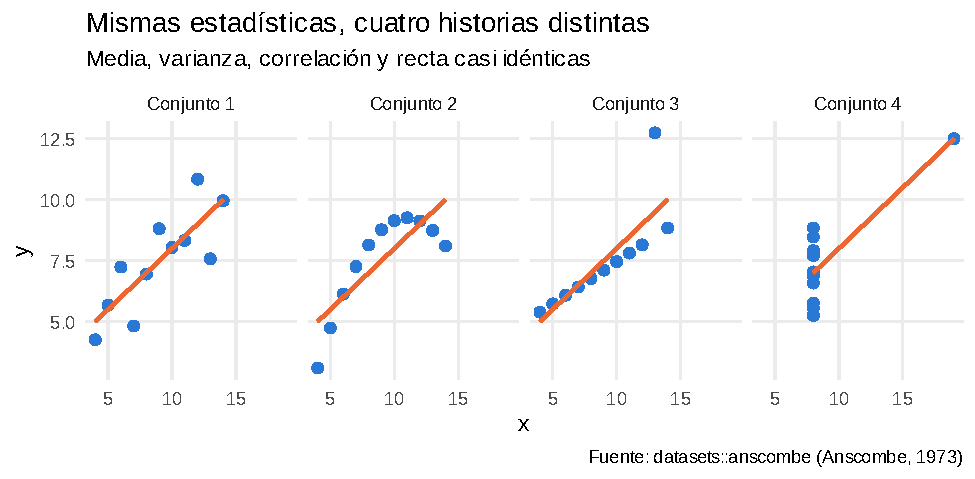
\includegraphics[width=0.95\textwidth]{m03-anscombe}
\caption{El cuarteto de Anscombe: cuatro conjuntos con estadísticas
idénticas y formas completamente distintas.}
\label{fig:m03-anscombe}
\end{figure}

\textbf{Cómo leerla.} El conjunto 1 es una relación lineal con ruido: la
recta sí lo describe. El conjunto 2 es una curva: una recta es el modelo
equivocado. En el conjunto 3 todos los puntos caen sobre una recta perfecta
salvo uno, un \termino{valor atípico} (\emph{outlier}) que jala la recta
hacia arriba. En el conjunto 4 casi todos los puntos tienen el mismo $x$ y un
solo punto extremo fabrica toda la ``correlación''. La lección para un
analista de BI es directa: \textbf{antes de reportar un promedio o una
correlación, grafica los datos}.

\begin{negocio}{El promedio que escondía dos tiendas}
Una cadena reporta que el ticket promedio de sus tiendas es de \$950 y que
es ``estable''. Al graficar la distribución de tickets por tienda aparece que
una sucursal tiene muchísimas compras pequeñas y unas cuantas enormes
(clientes mayoristas). El promedio era el mismo, pero la operación, el
riesgo y la estrategia comercial son completamente distintos. Solo la
gráfica lo hizo evidente.
\end{negocio}

\subsection{Visualización exploratoria contra explicativa}

En tu trabajo harás dos tipos de gráficas muy diferentes:

\begin{itemize}
  \item \termino{Visualización exploratoria}: gráficas rápidas que haces
        \emph{para ti} mientras analizas. No necesitan título bonito ni
        colores corporativos; necesitan ser rápidas. Harás decenas y
        tirarás casi todas. El objetivo es \emph{descubrir}.
  \item \termino{Visualización explicativa}: la gráfica que llevas a la
        dirección. Tiene \emph{un} mensaje, un título que lo dice
        (``Belleza cayó 41\% en el segundo semestre'' en vez de ``Ventas por
        categoría''), formato de negocio en los ejes, la fuente de los datos
        y nada que distraiga. El objetivo es \emph{comunicar}.
\end{itemize}

\begin{consejo}
Un buen título explicativo es una \emph{conclusión}, no una descripción.
Compara ``Ingresos mensuales 2023'' con ``7 de 12 meses superaron la meta''.
El segundo le ahorra al director el trabajo de interpretar la gráfica. El
subtítulo puede decir qué se mide (``Ingresos mensuales, MXN'').
\end{consejo}

% ----------------------------------------------------------------------------
\section{La gramática de gráficos}
\label{sec:m3-gramatica}

\paquete{ggplot2} se basa en la \termino{gramática de gráficos}
(\emph{grammar of graphics}), una idea de Leland Wilkinson que Hadley Wickham
implementó en R: toda gráfica estadística se puede describir como la suma de
unas cuantas piezas independientes. En vez de elegir ``un tipo de
gráfica'' de un menú (como en Excel), \emph{construyes} la gráfica
declarando cada pieza.

\begin{figure}[H]
\centering
\begin{tikzpicture}[
  capa/.style={draw=#1, fill=#1!10, rounded corners=2pt,
               minimum width=4.2cm, minimum height=0.62cm,
               font=\sffamily\small\bfseries, text=#1},
  expl/.style={font=\sffamily\footnotesize, text=gristexto, anchor=west,
               align=left},
  fun/.style={font=\ttfamily\footnotesize, text=codigoinline, anchor=east}]
  \node[capa=primario]   (dat) at (0,0)    {1. Datos};
  \node[capa=secundario] (aes) at (0,0.75) {2. Estéticas (aes)};
  \node[capa=exito]      (geo) at (0,1.5)  {3. Geometrías (geom)};
  \node[capa=acento]     (esc) at (0,2.25) {4. Escalas (scale)};
  \node[capa=morado]     (fac) at (0,3.0)  {5. Facetas (facet)};
  \node[capa=peligro]    (coo) at (0,3.75) {6. Coordenadas (coord)};
  \node[capa=gristexto]  (tem) at (0,4.5)  {7. Tema (theme, labs)};
  \node[expl] at (2.4,0)    {La tabla: una fila por observación};
  \node[expl] at (2.4,0.75) {Qué columna va a $x$, $y$, color, tamaño\ldots};
  \node[expl] at (2.4,1.5)  {Cómo se dibuja: puntos, barras, líneas\ldots};
  \node[expl] at (2.4,2.25) {Cómo se traduce el dato: \$, \%, colores, log};
  \node[expl] at (2.4,3.0)  {Dividir en paneles pequeños};
  \node[expl] at (2.4,3.75) {Sistema de ejes: normal, invertido, zoom};
  \node[expl] at (2.4,4.5)  {Títulos, fuentes, cuadrícula, leyenda};
  \node[fun] at (-2.3,0)    {ggplot(datos)};
  \node[fun] at (-2.3,0.75) {aes(x, y)};
  \node[fun] at (-2.3,1.5)  {geom\_col()};
  \node[fun] at (-2.3,2.25) {scale\_y\_continuous()};
  \node[fun] at (-2.3,3.0)  {facet\_wrap()};
  \node[fun] at (-2.3,3.75) {coord\_cartesian()};
  \node[fun] at (-2.3,4.5)  {theme\_minimal()};
  \draw[-{Stealth[length=2.5mm]}, thick, acento] (8.9,0) -- (8.9,4.5)
     node[midway, right, font=\sffamily\scriptsize, text=acento,
          align=left] {se suman\\con \texttt{+}};
\end{tikzpicture}
\caption{Las siete capas de la gramática de gráficos. Solo las tres
primeras son obligatorias; las demás tienen valores por defecto.}
\label{fig:m3-capas}
\end{figure}

Las capas se combinan con el signo \codigo{+}. Una gráfica mínima necesita
solo las tres primeras: \emph{datos}, \emph{estéticas} y al menos una
\emph{geometría}. Todo lo demás (escalas, facetas, coordenadas, tema) tiene
un valor por defecto razonable que puedes cambiar.

\begin{concepto}{Estética (aes)}
Una \termino{estética} es una propiedad visual que \emph{depende de los
datos}: la posición en $x$, la posición en $y$, el color, el relleno
(\codigo{fill}), el tamaño, la forma, la transparencia (\codigo{alpha}).
Dentro de \codigo{aes()} dices ``esta columna controla esta propiedad''.
Si quieres que \emph{todas} las barras sean azules, eso no depende de los
datos y va \emph{fuera} de \codigo{aes()}:
\codigo{geom\_col(fill = "\#2a78d6")}.
\end{concepto}

\subsection{Los datos del módulo}

Trabajaremos sobre todo con \archivo{transacciones.csv} (1,000 tickets de
2023), unida al catálogo de productos (para tener la categoría) y a las
tiendas (para tener el nombre). Es el mismo \emph{join} que hiciste en el
Módulo~\ref{cap:manipulacion}.

\begin{rcode}
transacciones <- read_csv("datasets/transacciones.csv",
                          show_col_types = FALSE)
productos <- read_csv("datasets/productos.csv", show_col_types = FALSE)
tiendas   <- read_csv("datasets/tiendas.csv", show_col_types = FALSE)

ventas_detalle <- transacciones %>%
  left_join(select(productos, producto_id, categoria),
            by = "producto_id") %>%
  left_join(select(tiendas, tienda_id, nombre_tienda),
            by = "tienda_id") %>%
  # "Sucursal Outlet" -> "Outlet": etiquetas más cortas para las gráficas
  mutate(tienda = str_remove(nombre_tienda, "Sucursal "))

ventas_detalle %>%
  select(fecha, categoria, tienda, metodo_pago, total_transaccion) %>%
  head(4)
\end{rcode}
\begin{rsalida}
PENDIENTE
\end{rsalida}

Para la primera gráfica necesitamos los ingresos de cada mes.
\codigo{floor\_date(fecha, unit = "month")} (de \paquete{lubridate}) lleva
cada fecha al primer día de su mes: así obtenemos una columna de tipo
\emph{fecha}, no de texto, lo que será importante para el eje $x$.

\begin{rcode}
ventas_mes <- ventas_detalle %>%
  mutate(mes = floor_date(fecha, unit = "month")) %>%
  group_by(mes) %>%
  summarise(ingresos = sum(total_transaccion),
            tickets  = n(),
            .groups  = "drop")
ventas_mes
\end{rcode}
\begin{rsalida}
PENDIENTE
\end{rsalida}

\subsection{Tu primer gráfico, capa por capa}

\textbf{Pregunta de negocio:} ¿cómo evolucionaron los ingresos mes a mes en
2023? Construiremos la respuesta en cuatro pasos y guardaremos cada paso en
un objeto para ver cómo cambia.

\begin{rcode}
# Paso 1: datos + estéticas. Solo el "lienzo" con los ejes
paso1 <- ggplot(data = ventas_mes, mapping = aes(x = mes, y = ingresos))
paso1
\end{rcode}

\codigo{ggplot()} crea el lienzo. Con \codigo{aes(x = mes, y = ingresos)}
le dices qué columna va en cada eje. R ya calcula los rangos (de enero a
diciembre; de unos \$57,000 a \$96,000) pero no dibuja nada, porque aún no
hay geometría.

\begin{rcode}
# Paso 2: + una geometría de línea (color y grosor fijos, fuera de aes)
paso2 <- paso1 + geom_line(color = "#2a78d6", linewidth = 0.8)
paso2
\end{rcode}

Al \emph{sumar} \codigo{geom\_line()} aparece la línea. El color y el grosor
(\codigo{linewidth}) son constantes, por eso van como argumentos de la
geometría y no dentro de \codigo{aes()}.

\begin{rcode}
# Paso 3: + puntos en cada mes y + escala del eje y en dólares
paso3 <- paso2 +
  geom_point(color = "#2a78d6", size = 2) +
  scale_y_continuous(labels = dollar)
paso3
\end{rcode}

Las capas se apilan: \codigo{geom\_point()} dibuja encima de la línea. La
\emph{escala} \codigo{scale\_y\_continuous(labels = dollar)} no cambia los
datos, solo cómo se \emph{muestran} los números del eje: 90000 se vuelve
\$90,000.

\begin{rcode}
# Paso 4: + títulos y + un tema limpio
paso4 <- paso3 +
  labs(title = "Ingresos mensuales 2023", x = NULL, y = "Ingresos") +
  theme_minimal() +
  theme(panel.grid.minor = element_blank())
paso4
\end{rcode}

\codigo{labs()} pone los textos (\codigo{x = NULL} quita el título del eje
$x$, porque ``mes'' es obvio). \codigo{theme\_minimal()} quita el fondo gris
y \codigo{theme(panel.grid.minor = element\_blank())} elimina las líneas
secundarias de la cuadrícula, que solo agregan ruido. La
figura~\ref{fig:m03-pasos} muestra los cuatro pasos.

\begin{figure}[H]
\centering
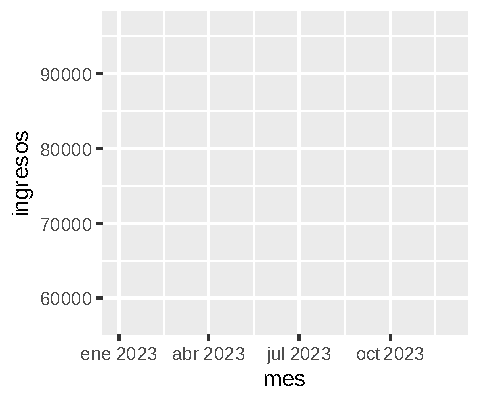
\includegraphics[width=0.48\textwidth]{m03-paso-1}\hfill
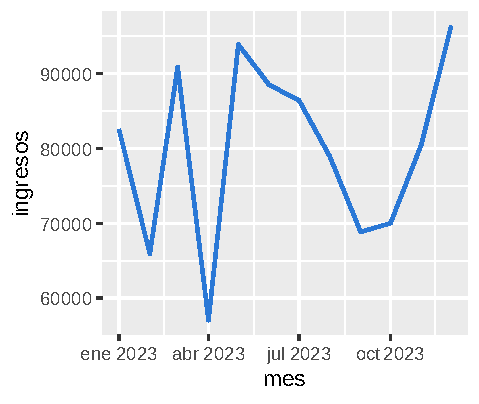
\includegraphics[width=0.48\textwidth]{m03-paso-2}\\[4pt]
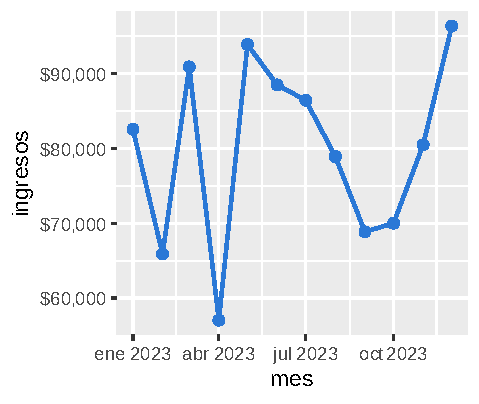
\includegraphics[width=0.48\textwidth]{m03-paso-3}\hfill
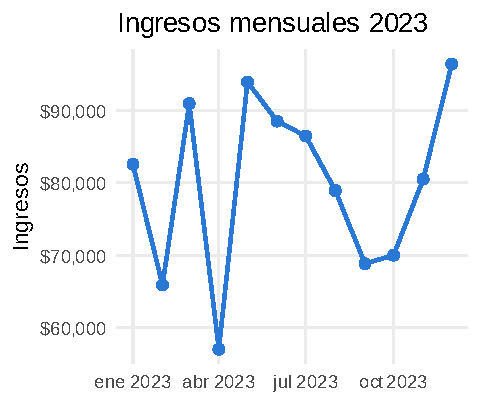
\includegraphics[width=0.48\textwidth]{m03-paso-4}
\caption{La misma gráfica en cuatro pasos: lienzo (arriba a la izquierda),
línea, puntos con escala en dólares y, finalmente, títulos y tema.}
\label{fig:m03-pasos}
\end{figure}

\textbf{Cómo leerla.} Ya con el paso 4 se ve la historia del año: dos caídas
fuertes (febrero y, sobre todo, abril), una meseta alta de mayo a julio, un
bache en septiembre--octubre y un cierre muy fuerte en diciembre.

\begin{advertencia}
El \codigo{+} va \textbf{al final} de cada línea, nunca al principio de la
siguiente. Si escribes el \codigo{+} al inicio, R da por terminada la
instrucción en la línea anterior y luego no sabe qué hacer con el
\codigo{+} suelto. Tampoco uses \codigo{\%>\%} entre capas de
\paquete{ggplot2}: el pipe sirve para \emph{transformar datos}; el \codigo{+}
para \emph{añadir capas}. Verás ambos errores en la
sección~\ref{sec:m3-errores}.
\end{advertencia}

\begin{hazlotu}
Repite los cuatro pasos pero con \codigo{y = tickets} (número de tickets por
mes) y el título ``Tickets por mes 2023''. Pista: en el paso 3 cambia
\codigo{dollar} por \codigo{comma}. ¿Coinciden los meses bajos con los de
ingresos?
\end{hazlotu}

% ----------------------------------------------------------------------------
\section{Elegir la gráfica correcta}
\label{sec:m3-elegir}

Antes de escribir código pregúntate: \emph{¿qué quiero que vea quien mire la
gráfica?} La respuesta casi siempre cae en una de seis familias
(tabla~\ref{tab:m3-elegir}).

\begin{table}[H]
\centering
\small
\caption{¿Qué quieres mostrar? Gráfica recomendada y qué evitar.}
\label{tab:m3-elegir}
\begin{tabularx}{\textwidth}{>{\raggedright\arraybackslash}p{2.6cm}
  >{\raggedright\arraybackslash}X >{\raggedright\arraybackslash}X}
\toprule
\textbf{Quiero mostrar\ldots} & \textbf{Gráfica recomendada} &
\textbf{Evita} \\
\midrule
Comparación entre categorías (tiendas, productos) &
Barras ordenadas; horizontales si los nombres son largos
(\codigo{geom\_col()}) &
Barras de colores sin significado; pasteles; ejes que no empiezan en 0 \\
Evolución en el tiempo (meses, semanas) &
Línea (\codigo{geom\_line()}); barras si son pocos periodos &
Más de 4--5 líneas de colores; doble eje Y \\
Distribución (cómo se reparten los tickets) &
Histograma, densidad, boxplot (\codigo{geom\_histogram()},
\codigo{geom\_boxplot()}) &
Reportar solo el promedio \\
Relación entre dos medidas (precio y cantidad) &
Dispersión (\codigo{geom\_point()}) con tendencia opcional &
Unir los puntos con líneas; más de 3 colores de grupo \\
Composición (partes de un total) &
Barras 100\% o barras de participación; pastel solo con 2--3 porciones &
Pastel de 10 rebanadas; dona 3D \\
Un solo número (ingresos del año) &
Tarjeta KPI: el número grande con su contexto &
Una gráfica con una sola barra \\
\bottomrule
\end{tabularx}
\end{table}

\begin{concepto}{Tarjeta KPI}
Un \termino{KPI} (\emph{Key Performance Indicator}, indicador clave de
desempeño) es un número que resume el desempeño: ingresos, tickets, ticket
promedio. Cuando el mensaje es \emph{un} número, la mejor visualización es
una \termino{tarjeta KPI}: el número grande, una etiqueta y, si acaso, la
comparación contra la meta o el año anterior. Una gráfica con una sola barra
ocupa más espacio y comunica menos.
\end{concepto}

\begin{hazlotu}
Para cada pregunta, decide la familia de la tabla~\ref{tab:m3-elegir}:
(a) ``¿qué vendedor vendió más?'', (b) ``¿cuánto vendimos en total?'',
(c) ``¿los clientes jóvenes gastan más por ticket?'', (d) ``¿cómo se
reparten los ingresos entre los métodos de pago?''.
\end{hazlotu}



\part{Nivel intermedio}
% ============================================================================
% MÓDULO 4. ANÁLISIS EXPLORATORIO Y ESTADÍSTICA PARA NEGOCIOS
% ============================================================================
\chapter{Análisis exploratorio y estadística para negocios}
\label{cap:eda}

\begin{objetivos}
\begin{itemize}
  \item Aplicar un proceso ordenado de \termino{análisis exploratorio de datos}
        (EDA) con una lista de verificación que puedes reutilizar en cualquier
        proyecto.
  \item Calcular e interpretar medidas de tendencia central, dispersión,
        percentiles y forma de una distribución, y saber cuándo el promedio
        engaña.
  \item Detectar datos atípicos con reglas objetivas y decidir qué hacer con
        ellos sin borrarlos a ciegas.
  \item Construir KPIs de desempeño (crecimiento, acumulados, promedios
        móviles, índices y avance contra meta) y un análisis de Pareto/ABC.
  \item Medir relaciones con correlaciones y distinguir correlación de
        causalidad.
  \item Usar las distribuciones normal, binomial y de Poisson para responder
        preguntas de probabilidad del día a día.
  \item Estimar con intervalos de confianza, aplicar pruebas de hipótesis
        (t, proporciones, ANOVA, chi-cuadrada) y ajustar regresiones lineales,
        explicando los resultados en lenguaje de negocio.
\end{itemize}
\end{objetivos}

Imagina que trabajas como analista en una cadena de tiendas con diez
sucursales en México. Es lunes y la directora comercial te escribe:
\emph{``Antes de aprobar el presupuesto de fin de año necesito entender qué
está pasando con las ventas: ¿cuánto gasta un cliente típico?, ¿hay tiendas
que funcionen mejor que otras?, ¿nuestros clientes premium realmente gastan
más?, ¿qué productos sostienen el negocio? Y si invertimos más en publicidad,
¿cuánto deberíamos esperar vender?''}.

Con lo que aprendiste en los Módulos~\ref{cap:manipulacion}
y~\ref{cap:visualizacion} ya puedes filtrar, agrupar, unir tablas y graficar.
Pero la directora no quiere tablas sueltas: quiere \emph{respuestas}. Para
darlas necesitas dos cosas. La primera es un \textbf{método} para recorrer los
datos sin perderte: eso es el análisis exploratorio. La segunda es la
\textbf{estadística}, que te permite distinguir un patrón real de una simple
casualidad y decir con honestidad cuánta confianza tienes en cada número.

En este módulo aprenderás ambas cosas con los datos del curso. No necesitas
saber matemáticas avanzadas: cada fórmula aparece explicada en palabras, se
calcula en R paso a paso y termina con la pregunta que más importa en una
empresa: \emph{¿y esto qué significa para el negocio?}

% ----------------------------------------------------------------------------
\section{¿Qué es el análisis exploratorio (EDA)?}
\label{sec:m4-eda}

\begin{concepto}{Análisis exploratorio de datos (EDA)}
El \termino{análisis exploratorio de datos} (EDA, por sus siglas en inglés,
\emph{Exploratory Data Analysis}) es el proceso de conocer un conjunto de
datos \emph{antes} de sacar conclusiones: revisar su estructura, su calidad,
cómo se reparten los valores, cómo se relacionan las variables y qué
preguntas vale la pena investigar. El término lo popularizó el estadístico
John Tukey en 1977 con una idea sencilla: primero mira los datos, después
decide qué prueba aplicar.
\end{concepto}

Piensa en el EDA como la consulta de un médico: antes de recetar, toma la
presión, pregunta síntomas y pide análisis. Si te saltas ese paso, puedes
recetar el medicamento equivocado. En BI pasa lo mismo: un dashboard
construido sin EDA puede mostrar con mucha elegancia un número que está mal.

La figura~\ref{fig:m4-proceso} resume el proceso que seguiremos en todo el
módulo. No es una receta rígida: a menudo un hallazgo en el paso 5 te obliga a
volver al paso 2.

\begin{figure}[H]
\centering
\begin{tikzpicture}[
  paso/.style={draw=primario, fill=primario!6, rounded corners=3pt,
               minimum width=2.3cm, minimum height=1cm, align=center,
               font=\sffamily\footnotesize},
  flecha/.style={-{Stealth[length=2.5mm]}, thick, color=gristexto}]
  \node[paso] (p1) {1. Estructura};
  \node[paso, right=0.45cm of p1] (p2) {2. Calidad};
  \node[paso, right=0.45cm of p2] (p3) {3. Univariado};
  \node[paso, right=0.45cm of p3] (p4) {4. Bivariado};
  \node[paso, below=0.9cm of p4] (p5) {5. Segmentos};
  \node[paso, left=0.45cm of p5] (p6) {6. Atípicos};
  \node[paso, left=0.45cm of p6, fill=acento!10, draw=acento] (p7)
       {7. Hipótesis};
  \node[paso, left=0.45cm of p7, fill=exito!10, draw=exito] (p8)
       {Pregunta de\\negocio};
  \draw[flecha] (p1) -- (p2);
  \draw[flecha] (p2) -- (p3);
  \draw[flecha] (p3) -- (p4);
  \draw[flecha] (p4) -- (p5);
  \draw[flecha] (p5) -- (p6);
  \draw[flecha] (p6) -- (p7);
  \draw[flecha] (p7) -- (p8);
  \draw[flecha, dashed] (p8) -- (p1);
\end{tikzpicture}
\caption{Proceso de análisis exploratorio. La flecha punteada indica que cada
hipótesis genera nuevas preguntas y el ciclo se repite.}
\label{fig:m4-proceso}
\end{figure}

La tabla~\ref{tab:m4-checklist} convierte el proceso en una lista de
verificación. Te recomiendo copiarla en tus proyectos: evita que se te olvide
revisar algo importante.

\begin{table}[H]
\centering
\small
\caption{Lista de verificación (\emph{checklist}) del análisis exploratorio.}
\label{tab:m4-checklist}
\begin{tabularx}{\textwidth}{@{}l X l@{}}
\toprule
\textbf{Paso} & \textbf{Pregunta que respondes} & \textbf{Funciones de R} \\
\midrule
1. Estructura & ¿Cuántas filas y columnas hay? ¿Qué tipo tiene cada
  columna? ¿Qué representa cada fila? & \codigo{dim()}, \codigo{glimpse()} \\
2. Calidad & ¿Hay valores faltantes, duplicados, negativos imposibles o
  categorías mal escritas? & \codigo{skim()}, \codigo{summary()},
  \codigo{count()} \\
3. Univariado & ¿Cómo se reparte cada variable? ¿Cuál es su valor típico y
  cuánto varía? & \codigo{mean()}, \codigo{quantile()},
  \codigo{geom\_histogram()} \\
4. Bivariado & ¿Qué variables se mueven juntas? & \codigo{cor()},
  \codigo{geom\_point()} \\
5. Segmentos & ¿Cambian los resultados por tienda, categoría o tipo de
  cliente? & \codigo{group\_by()} + \codigo{summarise()} \\
6. Atípicos & ¿Hay valores extremos? ¿Son errores o casos valiosos? &
  \codigo{IQR()}, \codigo{geom\_boxplot()} \\
7. Hipótesis & ¿Qué diferencias parecen reales y cuáles pueden ser azar? &
  \codigo{t.test()}, \codigo{lm()} \\
\bottomrule
\end{tabularx}
\end{table}

\subsection{Preparar el entorno}

En este módulo usaremos dos paquetes nuevos: \paquete{skimr}, que resume un
data frame completo con una sola función, y \paquete{corrplot}, que dibuja
matrices de correlación. Instálalos una sola vez:

\begin{rnoejecutar}
install.packages(c("skimr", "corrplot"))
\end{rnoejecutar}

Ahora carga los paquetes y los datos. Recuerda que el directorio de trabajo
debe ser la carpeta del curso (la que contiene \archivo{datasets/}).

\begin{rcode}
# Paquetes del módulo
library(tidyverse)   # dplyr, ggplot2, readr, tidyr... (Módulos 2 y 3)
library(skimr)       # resúmenes rápidos de un data frame
library(corrplot)    # matrices de correlación
library(scales)      # formatos de negocio: dollar(), percent(), comma()

# Datos del curso
transacciones <- read_csv("datasets/transacciones.csv",
                          show_col_types = FALSE)
clientes  <- read_csv("datasets/clientes.csv", show_col_types = FALSE)
productos <- read_csv("datasets/productos.csv", show_col_types = FALSE)
tiendas   <- read_csv("datasets/tiendas.csv", show_col_types = FALSE)
\end{rcode}

También definimos los colores corporativos y el tema gráfico que construiste
en el Módulo~\ref{cap:visualizacion}, para que todas las gráficas del módulo
tengan el mismo estilo:

\begin{rcode}
# Colores corporativos
color_principal <- "#2a78d6"   # una sola serie
color_resalte   <- "#eb6834"   # para destacar un elemento
color_gris      <- "#b5b3ad"   # el resto, cuando se resalta uno
paleta_libro <- c("#2a78d6", "#eb6834", "#1baf7a", "#eda100",
                  "#e87ba4", "#008300", "#4a3aa7", "#e34948")

# Tema corporativo (misma forma que en el Módulo 3)
tema_libro <- function(base_size = 11) {
  theme_minimal(base_size = base_size) +
    theme(
      plot.title       = element_text(face = "bold", color = "#0b0b0b"),
      plot.subtitle    = element_text(color = "#52514e"),
      plot.caption     = element_text(color = "#52514e", size = rel(0.8)),
      axis.title       = element_text(color = "#52514e"),
      axis.text        = element_text(color = "#52514e"),
      panel.grid.minor = element_blank(),
      panel.grid.major = element_line(color = "#e6e5e1", linewidth = 0.3),
      legend.position  = "top",
      legend.title     = element_text(color = "#52514e")
    )
}
\end{rcode}

\subsection{Pasos 1 y 2: estructura y calidad}

Empieza siempre por lo básico: ¿qué tamaño tiene la tabla y qué contiene cada
columna?

\begin{rcode}
dim(transacciones)        # filas y columnas
glimpse(transacciones)    # tipo y primeros valores de cada columna
\end{rcode}
\begin{rsalida}
[1] 1000   14
Rows: 1,000
Columns: 14
$ transaccion_id    <dbl> 1, 2, 3, 4, 5, 6, 7, 8, 9, 10, 11, 12, 13,~
$ fecha             <date> 2023-01-13, 2023-01-09, 2023-02-20, 2023-~
$ hora              <time> 13:15:00, 10:45:00, 10:30:00, 10:45:00, 1~
$ cliente_id        <dbl> 155, 155, 75, 51, 173, 135, 90, 168, 13, 9~
$ producto_id       <dbl> 3, 47, 6, 17, 28, 46, 30, 48, 21, 12, 49, ~
$ cantidad          <dbl> 4, 4, 3, 4, 1, 2, 4, 2, 2, 5, 2, 3, 4, 2, ~
$ precio_venta      <dbl> 303.97, 58.07, 275.46, 105.28, 205.47, 534~
$ metodo_pago       <chr> "Tarjeta Crédito", "Tarjeta Débito", "Tarj~
$ tienda_id         <dbl> 10, 2, 7, 6, 7, 7, 8, 8, 5, 2, 7, 6, 8, 2,~
$ vendedor_id       <dbl> 4, 22, 14, 5, 14, 22, 23, 5, 3, 14, 5, 9, ~
$ total_transaccion <dbl> 1215.88, 232.28, 826.38, 421.12, 205.47, 1~
$ mes               <chr> "2023-01", "2023-01", "2023-02", "2023-05"~
$ trimestre         <chr> "Q1", "Q1", "Q1", "Q2", "Q1", "Q1", "Q2", ~
$ dia_semana        <chr> "viernes", "lunes", "lunes", "viernes", "m~
\end{rsalida}

Cada fila es una \emph{transacción} (una línea de venta): un cliente compró
cierta \codigo{cantidad} de un producto a un \codigo{precio\_venta} en una
tienda. La columna \codigo{total\_transaccion} es cantidad $\times$ precio.
Fíjate en que \codigo{read\_csv()} reconoció \codigo{fecha} como fecha
(\codigo{<date>}) y \codigo{hora} como hora (\codigo{<time>}); los
identificadores (\codigo{cliente\_id}, \codigo{tienda\_id}\ldots) son
números, pero en realidad son \emph{etiquetas}: promediarlos no tiene
sentido.

La función \codigo{summary()} da un primer resumen numérico. Aplícala solo a
las columnas de medida para que la salida sea legible:

\begin{rcode}
transacciones %>%
  select(cantidad, precio_venta, total_transaccion) %>%
  summary()
\end{rcode}
\begin{rsalida}
    cantidad      precio_venta    total_transaccion
 Min.   :1.000   Min.   : 20.14   Min.   :  22.65
 1st Qu.:2.000   1st Qu.:164.11   1st Qu.: 341.11
 Median :3.000   Median :324.92   Median : 713.49
 Mean   :2.969   Mean   :318.31   Mean   : 959.99
 3rd Qu.:4.000   3rd Qu.:468.00   3rd Qu.:1478.62
 Max.   :5.000   Max.   :598.81   Max.   :2992.35
\end{rsalida}

Para cada columna obtienes el mínimo (\codigo{Min.}), el primer cuartil
(\codigo{1st Qu.}), la mediana (\codigo{Median}), la media (\codigo{Mean}), el
tercer cuartil (\codigo{3rd Qu.}) y el máximo (\codigo{Max.}). Ya aparece una
pista importante: en \codigo{total\_transaccion} la media (959.99) es bastante
mayor que la mediana (713.49). En la sección~\ref{sec:m4-forma} verás que eso
indica una distribución con ``cola'' hacia los valores altos.

El paquete \paquete{skimr} va más allá: con \codigo{skim()} obtienes en una
sola llamada el número de faltantes (\codigo{n\_missing}), el porcentaje de
datos completos (\codigo{complete\_rate}), la media, la desviación estándar y
los percentiles de cada columna, agrupados por tipo de dato. En la consola de
RStudio, \codigo{skim()} dibuja además un mini histograma con caracteres
especiales; para un reporte impreso como este libro usamos su variante
\codigo{skim\_without\_charts()}, que muestra exactamente lo mismo sin ese
dibujo.

\begin{rcode}
skim_without_charts(transacciones)
\end{rcode}
\begin{rsalida}
-- Data Summary ------------------------
                           Values
Name                       transacciones
Number of rows             1000
Number of columns          14
_______________________
Column type frequency:
  character                4
  Date                     1
  difftime                 1
  numeric                  8
________________________
Group variables            None

-- Variable type: character ------------------------------------------
  skim_variable n_missing complete_rate min max empty n_unique
1 metodo_pago           0             1   8  15     0        4
2 mes                   0             1   7   7     0       12
3 trimestre             0             1   2   2     0        4
4 dia_semana            0             1   5   9     0        7
  whitespace
1          0
2          0
3          0
4          0

-- Variable type: Date -----------------------------------------------
  skim_variable n_missing complete_rate min        max
1 fecha                 0             1 2023-01-01 2023-12-31
  median     n_unique
1 2023-06-23      345

-- Variable type: difftime -------------------------------------------
  skim_variable n_missing complete_rate min        max
1 hora                  0             1 28800 secs 74700 secs
  median     n_unique
1 51300 secs       52

-- Variable type: numeric --------------------------------------------
  skim_variable     n_missing complete_rate   mean     sd   p0  p25
1 transaccion_id            0             1 500.   289.    1   251.
2 cliente_id                0             1  97.8   57.5   1    49
3 producto_id               0             1  25.3   14.4   1    13
4 cantidad                  0             1   2.97   1.45  1     2
5 precio_venta              0             1 318.   172.   20.1 164.
6 tienda_id                 0             1   5.61   2.88  1     3
7 vendedor_id               0             1  13.2    7.21  1     7
8 total_transaccion         0             1 960.   760.   22.6 341.
   p50    p75  p100
1 500.  750.  1000
2  97   150    200
3  25    37.2   50
4   3     4      5
5 325.  468.   599.
6   6     8     10
7  13    19     25
8 713. 1479.  2992.
\end{rsalida}

\begin{ejemplo}{Leer un \texttt{skim()} como analista}
¿Qué te dice esta salida en 30 segundos?
\begin{itemize}
  \item \textbf{Calidad}: \codigo{n\_missing} es 0 en todas las columnas y
        \codigo{complete\_rate} es 1: no hay faltantes. En datos reales casi
        nunca pasa; cuando veas un \codigo{complete\_rate} de 0.85, sabes que
        15\% de esa columna está vacía.
  \item \textbf{Categorías}: \codigo{metodo\_pago} tiene 4 valores distintos
        (\codigo{n\_unique}) y \codigo{mes}, 12. Si \codigo{metodo\_pago}
        tuviera 7 valores, sospecharías de errores de captura como
        ``tarjeta credito'' y ``Tarjeta Crédito''.
  \item \textbf{Cobertura}: las fechas van del 1 de enero al 31 de diciembre de
        2023, pero solo hay 345 fechas distintas: hubo días sin ninguna venta
        registrada.
  \item \textbf{Rangos}: \codigo{cantidad} va de 1 a 5 y el ticket
        (\codigo{total\_transaccion}) de 22.6 a 2,992; no hay negativos ni
        ceros imposibles.
\end{itemize}
\end{ejemplo}

\begin{hazlotu}
Aplica \codigo{skim\_without\_charts()} a \codigo{clientes} y a
\codigo{productos}. ¿Cuántos segmentos de edad hay? ¿Hay algún producto con
\codigo{margen\_pct} negativo? (Pista: mira el valor \codigo{p0}, que es el
mínimo.)
\end{hazlotu}

% ----------------------------------------------------------------------------
\section{Estadística descriptiva}
\label{sec:m4-descriptiva}

La \termino{estadística descriptiva} resume muchos datos en pocos números.
Responde dos preguntas: ¿cuál es el valor \emph{típico}? (tendencia central)
y ¿qué tanto se alejan los datos de ese valor típico? (dispersión). Para no
repetir \codigo{transacciones\$total\_transaccion} en cada línea, guardamos
esa columna en un vector llamado \codigo{ticket}:

\begin{rcode}
ticket <- transacciones$total_transaccion   # 1,000 tickets de venta
length(ticket)
\end{rcode}
\begin{rsalida}
[1] 1000
\end{rsalida}

\subsection{Medidas de tendencia central: media, mediana y moda}

La \termino{media} (o promedio) suma todos los valores y divide entre cuántos
son. Si llamamos $x_1, x_2, \ldots, x_n$ a los $n$ tickets:
\[
  \bar{x} \;=\; \frac{x_1 + x_2 + \cdots + x_n}{n}
          \;=\; \frac{1}{n}\sum_{i=1}^{n} x_i
\]
El símbolo $\sum$ (sigma) solo significa ``suma todo''. La \termino{mediana}
es el valor que queda justo a la mitad cuando ordenas los datos de menor a
mayor: la mitad de los tickets está por debajo y la otra mitad por encima. La
\termino{moda} es el valor que más se repite; es útil sobre todo para
variables categóricas (método de pago, día de la semana).

\begin{rcode}
media_ticket   <- mean(ticket)     # promedio
mediana_ticket <- median(ticket)   # valor central
media_ticket
mediana_ticket
sum(ticket) / length(ticket)       # la media "a mano": mismo resultado
\end{rcode}
\begin{rsalida}
[1] 959.9927
[1] 713.485
[1] 959.9927
\end{rsalida}

R no trae una función para la moda (la función \codigo{mode()} de R hace otra
cosa: dice el tipo de un objeto). La construimos nosotros con lo que
aprendiste en el Módulo~\ref{cap:fundamentos}:

\begin{rcode}
# Moda: el valor que más veces aparece en un vector
moda <- function(x) {
  frecuencias <- table(x)                      # cuenta cada valor
  names(frecuencias)[which.max(frecuencias)]   # el más frecuente
}

moda(transacciones$metodo_pago)   # método de pago más usado
moda(transacciones$dia_semana)    # día con más transacciones
moda(transacciones$cantidad)      # unidades más comunes por ticket
\end{rcode}
\begin{rsalida}
[1] "Tarjeta Crédito"
[1] "viernes"
[1] "1"
\end{rsalida}

\codigo{table()} cuenta cuántas veces aparece cada valor y
\codigo{which.max()} devuelve la posición del mayor conteo. La moda siempre
sale como texto (por eso \codigo{"1"} aparece entre comillas); si la
necesitas como número usa \codigo{as.numeric(moda(x))}. Si hay empate,
\codigo{which.max()} devuelve el primero en orden alfabético, así que
conviene revisar la tabla completa:

\begin{rcode}
table(transacciones$cantidad)
\end{rcode}
\begin{rsalida}
  1   2   3   4   5
219 196 190 187 208
\end{rsalida}

\begin{negocio}{La moda en la operación}
La moda responde preguntas operativas muy concretas: ¿cuál es la talla que más
se vende? (para surtir más), ¿cuál es el método de pago más usado? (para
negociar comisiones con el banco), ¿a qué hora llegan más clientes? (para
programar turnos). Aquí, la tarjeta de crédito es el método más frecuente y
lo más común es que un ticket lleve 1 sola unidad.
\end{negocio}

\subsection{Medidas de dispersión}

Dos tiendas pueden tener el mismo ticket promedio y comportarse de forma muy
distinta: en una todos gastan alrededor de 900 pesos y en la otra unos gastan
50 y otros 3,000. La \termino{dispersión} mide esa diferencia.

\begin{itemize}
  \item \termino{Rango}: máximo menos mínimo. Fácil, pero depende solo de dos
        datos (los más extremos).
  \item \termino{Varianza} ($s^2$): el promedio de las distancias al
        cuadrado respecto a la media. Elevamos al cuadrado para que las
        distancias negativas no cancelen a las positivas:
        \[ s^2 = \frac{1}{n-1}\sum_{i=1}^{n}(x_i - \bar{x})^2 \]
        Se divide entre $n-1$ y no entre $n$ por un ajuste técnico que
        corrige un pequeño sesgo cuando trabajas con muestras; con muchos
        datos la diferencia es mínima.
  \item \termino{Desviación estándar} ($s$): la raíz cuadrada de la
        varianza. Regresa a las unidades originales (pesos), por eso es la
        medida de dispersión más usada. Se interpreta como ``cuánto se aleja,
        típicamente, un dato del promedio''.
  \item \termino{Rango intercuartílico} (IQR): distancia entre el percentil
        75 y el 25. Mide la amplitud del 50\% central de los datos y no le
        afectan los extremos.
  \item \termino{Coeficiente de variación} (CV): la desviación estándar
        dividida entre la media, $CV = s/\bar{x}$. Como no tiene unidades,
        sirve para comparar la variabilidad de cosas distintas (tickets en
        pesos contra unidades vendidas).
\end{itemize}

\begin{rcode}
range(ticket)                  # mínimo y máximo
diff(range(ticket))            # rango = máximo - mínimo
var(ticket)                    # varianza (pesos al cuadrado)
sd(ticket)                     # desviación estándar (pesos)
IQR(ticket)                    # rango intercuartílico
sd(ticket) / mean(ticket)      # coeficiente de variación

# La varianza "a mano", para que veas que no hay magia:
sum((ticket - mean(ticket))^2) / (length(ticket) - 1)
\end{rcode}
\begin{rsalida}
[1]   22.65 2992.35
[1] 2969.7
[1] 578152.5
[1] 760.3634
[1] 1137.513
[1] 0.7920512
[1] 578152.5
\end{rsalida}

¿Qué nos dice esto? Un ticket típico se aleja unos \$760 del promedio de
\$960. El coeficiente de variación es 0.79: la desviación estándar equivale al
79\% de la media, lo que indica tickets \emph{muy} heterogéneos. Como regla
práctica, un CV menor a 0.15 indica datos bastante homogéneos, entre 0.15 y
0.30 variabilidad moderada y por encima de 0.30 alta variabilidad. La
varianza (578,152.5) está en ``pesos al cuadrado'', una unidad sin sentido de
negocio; por eso casi siempre reportarás la desviación estándar.

\begin{hazlotu}
Calcula el coeficiente de variación de \codigo{cantidad} y de
\codigo{precio\_venta}. ¿Cuál de las dos varía más en términos relativos?
\end{hazlotu}

\subsection{Percentiles y cuantiles}

El \termino{percentil} $p$ es el valor que deja por debajo al $p\%$ de los
datos. La mediana es el percentil 50; el primer y tercer
\termino{cuartil} son los percentiles 25 y 75. En R se calculan con
\codigo{quantile()}, indicando las proporciones que quieres:

\begin{rcode}
quantile(ticket, probs = c(0.10, 0.25, 0.50, 0.75, 0.90, 0.95))
\end{rcode}
\begin{rsalida}
      10%       25%       50%       75%       90%       95%
 159.1200  341.1125  713.4850 1478.6250 2113.6140 2501.2725
\end{rsalida}

Los percentiles se leen así: el 10\% de los tickets es menor a \$159.12; la
mitad, menor a \$713.49; y solo el 5\% supera \$2,501.27. Son perfectos para
fijar umbrales de negocio: si quieres un programa de beneficios para el 10\%
de compras más grandes, el corte está en \$2,113.61 (percentil 90).

\begin{ejemplo}{Umbral para un programa de lealtad}
La gerencia de mercadotecnia quiere regalar un cupón a los tickets que estén
en el 20\% más alto. ¿A partir de qué monto se entrega el cupón y cuántos
tickets del año lo habrían recibido?
\end{ejemplo}

\begin{rcode}
umbral_cupon <- quantile(ticket, probs = 0.80)   # percentil 80
umbral_cupon
sum(ticket > umbral_cupon)   # tickets que superan el umbral
\end{rcode}
\begin{rsalida}
     80%
1641.174
[1] 200
\end{rsalida}

El cupón se entregaría en compras mayores a \$1,641.17 y, con los datos de
2023, lo habrían recibido 200 tickets (el 20\% de 1,000, como era de
esperarse). Si cada cupón cuesta 50 pesos, el costo del programa sería de
unos 10,000 pesos al año.

\subsection{Cuándo la media engaña}
\label{sec:m4-media-engana}

La media tiene un defecto: \textbf{es muy sensible a los valores extremos}.
Un solo dato gigante la arrastra hacia arriba; la mediana, en cambio, apenas
se mueve. Veámoslo con dos ejemplos pequeños creados con \codigo{tibble()}.

\begin{ejemplo}{Un distribuidor con un cliente gigante}
Un distribuidor mayorista tiene 10 clientes. Nueve compran entre 20 y 30 mil
pesos al mes; el décimo es una cadena nacional que compra 900 mil. El
director pregunta: ``¿cuánto compra un cliente típico?''.
\end{ejemplo}

\begin{rcode}
compras_b2b <- tibble(
  cliente = paste("Cliente", 1:10),
  compra_mensual = c(22000, 25000, 21000, 28000, 30000,
                     24000, 26000, 23000, 27000, 900000)
)

compras_b2b %>%
  summarise(media   = mean(compra_mensual),
            mediana = median(compra_mensual))
\end{rcode}
\begin{rsalida}
# A tibble: 1 x 2
   media mediana
   <dbl>   <dbl>
1 112600   25500
\end{rsalida}

Si respondes ``un cliente típico compra 112,600 pesos'' estarás describiendo
a un cliente que no existe: nueve de diez compran menos de 31 mil. La mediana
(25,500) sí describe al cliente típico. La media sigue siendo útil para otra
pregunta: si multiplicas 112,600 por 10 clientes, obtienes exactamente las
ventas totales. \textbf{La media sirve para totales; la mediana, para
describir al caso típico.}

El segundo ejemplo es clásico en recursos humanos:

\begin{rcode}
salarios <- c(rep(15000, 9), 250000)   # 9 empleados y un director
mean(salarios)
median(salarios)
\end{rcode}
\begin{rsalida}
[1] 38500
[1] 15000
\end{rsalida}

Anunciar que ``el salario promedio en la empresa es de 38,500 pesos'' es
técnicamente cierto, pero engañoso: nueve de cada diez personas ganan 15,000.
Por eso las estadísticas oficiales de ingresos suelen reportar la mediana.

\begin{consejo}
Reporta siempre la media \emph{y} la mediana. Si son parecidas, los datos son
bastante simétricos y cualquiera sirve. Si la media es claramente mayor que la
mediana, hay valores altos que la arrastran: usa la mediana para describir el
caso típico y la media solo para calcular totales.
\end{consejo}

\subsection{Resumen estadístico por grupo}

En el Módulo~\ref{cap:manipulacion} aprendiste \codigo{group\_by()} +
\codigo{summarise()}. Ahora lo combinamos con todas las medidas anteriores
para comparar segmentos. Pregunta de negocio: \emph{¿el comportamiento del
ticket cambia según el método de pago?}

\begin{rcode}
resumen_pago <- transacciones %>%
  group_by(metodo_pago) %>%
  summarise(
    n        = n(),                                 # cuántos tickets
    ventas   = round(sum(total_transaccion)),       # total vendido
    media    = mean(total_transaccion),             # ticket promedio
    mediana  = median(total_transaccion),           # ticket típico
    desv_est = sd(total_transaccion),               # dispersión
    cv       = sd(total_transaccion) / mean(total_transaccion),
    .groups = "drop"
  ) %>%
  mutate(pct_ventas = ventas / sum(ventas)) %>%     # % de las ventas
  arrange(desc(ventas))

resumen_pago
\end{rcode}
\begin{rsalida}
# A tibble: 4 x 8
  metodo_pago         n ventas media mediana desv_est    cv pct_ventas
  <chr>           <int>  <dbl> <dbl>   <dbl>    <dbl> <dbl>      <dbl>
1 Tarjeta Crédito   350 351171 1003.    780.     782. 0.779     0.366
2 Efectivo          315 303735  964.    710.     757. 0.785     0.316
3 Tarjeta Débito    233 220855  948.    732.     738. 0.779     0.230
4 Transferencia     102  84232  826.    608.     741. 0.897     0.0877
\end{rsalida}

Lectura de negocio: la tarjeta de crédito concentra la mayor parte de las
ventas (36.6\%) y tiene el ticket promedio más alto (\$1,003); la
transferencia es el método menos usado y el de ticket más bajo (\$826). Los
cuatro métodos tienen un CV alto (de 0.78 a 0.90): en todos conviven tickets
muy pequeños y muy grandes. ¿La diferencia entre \$1,003 y \$826 es real o es azar? No lo
sabemos todavía: en la sección~\ref{sec:m4-hipotesis} aprenderás a
responderlo con una prueba de hipótesis.

\begin{hazlotu}
Repite el resumen agrupando por \codigo{tienda\_id}. ¿Qué tienda tiene la
mediana de ticket más alta? ¿Coincide con la que tiene la media más alta?
\end{hazlotu}

% ----------------------------------------------------------------------------
\section{Forma de la distribución}
\label{sec:m4-forma}

Los números resumen ayudan, pero nada sustituye a \emph{ver} los datos. La
\termino{distribución} de una variable describe qué valores toma y con qué
frecuencia. Su herramienta básica es el \termino{histograma}: divide el eje en
intervalos y cuenta cuántos datos caen en cada uno. Encima podemos dibujar una
\termino{curva de densidad}, una versión suavizada del histograma que deja
ver la forma general sin el ``ruido'' de las barras.

\begin{ejemplo}{¿Cómo se reparte el ticket de compra?}
La directora quiere saber si ``el ticket típico'' es un buen resumen o si hay
grupos de clientes con compras muy distintas. Dibujamos el histograma del
ticket con su curva de densidad y marcamos la media y la mediana.
\end{ejemplo}

\begin{rcode}
p_hist <- ggplot(transacciones, aes(x = total_transaccion)) +
  # barras: cuántos tickets caen en cada intervalo de 150 pesos
  geom_histogram(binwidth = 150, boundary = 0,
                 fill = color_principal, color = "white", alpha = 0.85) +
  # densidad reescalada (x 150) para que quede en la escala de las barras
  geom_density(aes(y = after_stat(count) * 150),
               color = "#0b0b0b", linewidth = 0.8) +
  # media (línea continua) y mediana (línea punteada)
  geom_vline(xintercept = media_ticket, color = color_resalte,
             linewidth = 0.8) +
  geom_vline(xintercept = mediana_ticket, color = color_resalte,
             linewidth = 0.8, linetype = "dashed") +
  annotate("text", x = media_ticket + 50, y = 140, hjust = 0,
           label = paste("Media:", dollar(media_ticket)),
           color = color_resalte, size = 3.5) +
  annotate("text", x = mediana_ticket - 50, y = 140, hjust = 1,
           label = paste("Mediana:", dollar(mediana_ticket)),
           color = color_resalte, size = 3.5) +
  scale_x_continuous(labels = dollar) +
  labs(title = "Distribución del ticket por transacción",
       subtitle = "Muchos tickets pequeños y una cola larga a la derecha",
       x = "Total de la transacción", y = "Número de transacciones") +
  tema_libro()

p_hist
\end{rcode}

\begin{figure}[H]
\centering
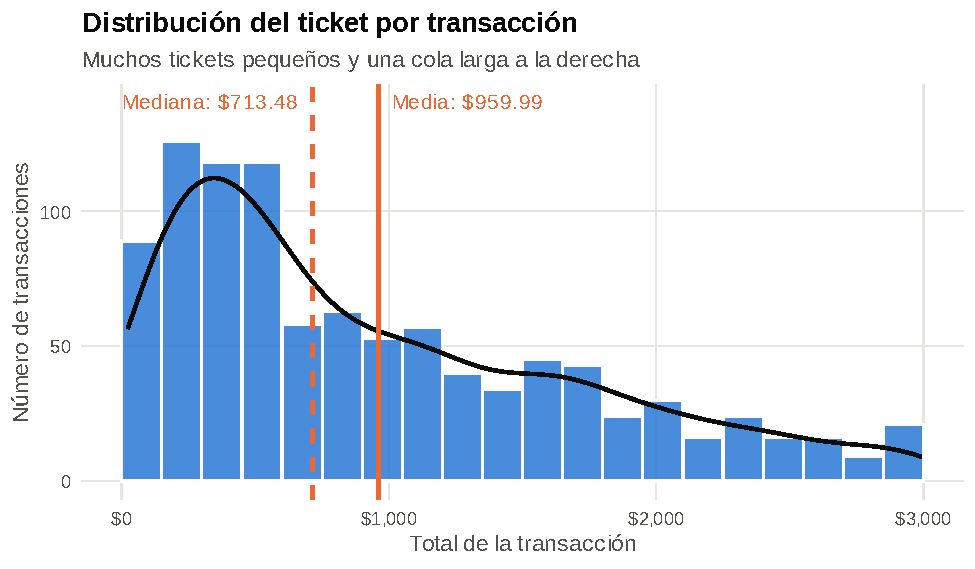
\includegraphics[width=0.9\textwidth]{m04-histograma-ticket}
\caption{Histograma y curva de densidad del ticket. La media queda a la
derecha de la mediana porque los tickets grandes la ``jalan''.}
\label{fig:m04-histograma-ticket}
\end{figure}

La figura~\ref{fig:m04-histograma-ticket} confirma lo que sugerían los
números: la mayoría de los tickets se concentra por debajo de 600 pesos y, a
partir de ahí, las barras bajan poco a poco formando una \termino{cola}
larga hacia la derecha. A esa forma se le llama \termino{asimetría
positiva} (o sesgo a la derecha). Observa que la media queda a la derecha de
la mediana: los pocos tickets grandes la arrastran.

\begin{consejo}
El ancho de las barras (\codigo{binwidth}) cambia mucho la impresión que da un
histograma. Prueba siempre dos o tres anchos distintos antes de sacar
conclusiones; con barras muy anchas se esconden patrones y con barras muy
angostas todo parece ruido.
\end{consejo}

\subsection{Medir la asimetría}

Podemos resumir la forma con un número: el \termino{coeficiente de
asimetría}. La idea es promediar las distancias a la media \emph{elevadas al
cubo}. Al elevar al cubo se conserva el signo (las distancias negativas
siguen siendo negativas) y los valores lejanos pesan muchísimo; si la cola
derecha es más larga, dominan los cubos positivos. Para que no dependa de las
unidades, se divide entre $s^3$:
\[
  \text{asimetría} \;=\;
  \frac{\frac{1}{n}\sum_{i=1}^{n}(x_i - \bar{x})^3}{s^3}
\]

\begin{rcode}
# Coeficiente de asimetría (versión sencilla)
asimetria <- function(x) {
  mean((x - mean(x))^3) / sd(x)^3
}

asimetria(ticket)                        # ticket de compra
asimetria(transacciones$precio_venta)    # precio unitario
asimetria(compras_b2b$compra_mensual)    # distribuidor con cliente gigante
\end{rcode}
\begin{rsalida}
[1] 0.8711898
[1] -0.08471191
[1] 2.276413
\end{rsalida}

La tabla~\ref{tab:m4-asimetria} te ayuda a interpretarlo. El ticket tiene una
asimetría de 0.87 (positiva y moderada); el precio unitario está muy cerca de
cero (los precios se reparten de forma pareja entre 20 y 600 pesos); y el
ejemplo del distribuidor, con un cliente gigante, tiene una asimetría fuerte
de 2.28.

\begin{table}[H]
\centering
\small
\caption{Cómo interpretar el coeficiente de asimetría.}
\label{tab:m4-asimetria}
\begin{tabularx}{\textwidth}{@{}l X X@{}}
\toprule
\textbf{Valor} & \textbf{Forma} & \textbf{Ejemplo de negocio} \\
\midrule
Entre $-0.5$ y $0.5$ & Aproximadamente simétrica; media $\approx$ mediana &
  Estatura de clientes, tiempos de entrega estables \\
Entre $0.5$ y $1$ & Asimetría positiva moderada & Ticket de compra de
  este módulo \\
Mayor a $1$ & Asimetría positiva fuerte (cola derecha larga) & Ingresos de
  clientes, ventas por producto en catálogos grandes \\
Menor a $-0.5$ & Asimetría negativa (cola izquierda) & Calificaciones de
  satisfacción cuando casi todos ponen 9 o 10 \\
\bottomrule
\end{tabularx}
\end{table}

\begin{negocio}{El ticket con cola larga}
Una distribución con cola larga a la derecha es la norma en el comercio: hay
muchas compras chicas y pocas muy grandes. Esto tiene tres consecuencias
prácticas:
\begin{enumerate}
  \item \textbf{Metas}: si fijas la meta del ticket con la media, la mayoría
        de los vendedores quedarán por debajo aunque trabajen bien; la mediana
        es una referencia más justa para el ``vendedor típico''.
  \item \textbf{Estrategia}: la cola derecha son los clientes que más valen.
        Identificarlos (percentil 90 o 95) permite diseñar atención
        preferente.
  \item \textbf{Oportunidad}: el gran bloque de tickets bajos es el terreno
        para estrategias de venta cruzada (``¿le agrego\ldots?'') que suban el
        ticket típico.
\end{enumerate}
\end{negocio}

\begin{hazlotu}
Dibuja el histograma de \codigo{precio\_venta} con \codigo{binwidth = 50} y
calcula su asimetría. ¿Se parece a la forma del ticket? ¿Por qué crees que el
ticket (cantidad $\times$ precio) tiene cola y el precio no?
\end{hazlotu}

% ----------------------------------------------------------------------------
\section{Datos atípicos (outliers)}
\label{sec:m4-atipicos}

Un \termino{dato atípico} (en inglés, \emph{outlier}) es un valor que se
aleja mucho del resto. Puede ser un \textbf{error} (alguien tecleó 29,923.50
en vez de 2,992.35), un \textbf{caso legítimo pero excepcional} (una empresa
que compró 50 laptops) o una \textbf{señal de fraude}. El trabajo del analista
no es borrarlo: es \emph{detectarlo, investigarlo y decidir}.

\subsection{Regla de 1.5 $\times$ IQR}

La regla más usada la propuso también John Tukey y es la que dibujan los
diagramas de caja (\emph{boxplots}). Se consideran atípicos los valores que
caen fuera de estas ``cercas'':
\[
  \text{límite inferior} = Q_1 - 1.5 \times IQR
  \qquad\qquad
  \text{límite superior} = Q_3 + 1.5 \times IQR
\]
donde $Q_1$ y $Q_3$ son los percentiles 25 y 75, e $IQR = Q_3 - Q_1$. Como
usa percentiles, la regla no se deja engañar por los propios atípicos.

\begin{rcode}
q1  <- quantile(ticket, 0.25)
q3  <- quantile(ticket, 0.75)
iqr <- q3 - q1
limite_inferior <- unname(q1 - 1.5 * iqr)   # unname() quita el "25%"
limite_superior <- unname(q3 + 1.5 * iqr)
c(limite_inferior, limite_superior)

# ¿Cuántos tickets quedan fuera de las cercas?
sum(ticket < limite_inferior | ticket > limite_superior)
\end{rcode}
\begin{rsalida}
[1] -1365.156  3184.894
[1] 0
\end{rsalida}

Ningún ticket es atípico según esta regla: el límite superior (\$3,184.89)
está por encima del ticket máximo (\$2,992.35). Tiene sentido: una transacción
tiene como máximo 5 unidades de un producto de hasta 600 pesos. El límite
inferior es negativo, lo cual simplemente significa que por abajo no hay
forma de ser atípico. \textbf{``No hay atípicos'' también es un resultado
valioso}: significa que puedes usar los tickets con tranquilidad.

\subsection{Puntuación z}

La segunda regla usa la \termino{puntuación z} (\emph{z-score}): cuántas
desviaciones estándar se aleja cada dato de la media.
\[
  z_i = \frac{x_i - \bar{x}}{s}
\]
Un $z = 2$ significa ``dos desviaciones estándar por encima del promedio''.
Se suele marcar como atípico todo dato con $|z| > 3$.

\begin{rcode}
z_ticket <- (ticket - mean(ticket)) / sd(ticket)
range(z_ticket)              # el z más bajo y el más alto
sum(abs(z_ticket) > 3)       # tickets con |z| > 3
\end{rcode}
\begin{rsalida}
[1] -1.232756  2.672876
[1] 0
\end{rsalida}

El ticket más alto está a 2.67 desviaciones estándar de la media: tampoco hay
atípicos por esta regla. Para reutilizar la regla del IQR la convertimos en
función:

\begin{rcode}
# Devuelve TRUE para los valores fuera de las cercas de Tukey
marcar_atipicos <- function(x) {
  q1 <- quantile(x, 0.25, na.rm = TRUE)
  q3 <- quantile(x, 0.75, na.rm = TRUE)
  rango_iq <- q3 - q1
  x < q1 - 1.5 * rango_iq | x > q3 + 1.5 * rango_iq
}
\end{rcode}

\subsection{Cuando los atípicos son errores}

Para ver las reglas en acción con errores de verdad, \textbf{simulamos} una
situación frecuente: al exportar del punto de venta se colaron tres registros
problemáticos. Agregamos a una copia de los tickets una venta con el punto
decimal recorrido (29,923.50), una devolución capturada como venta negativa
($-450$) y un ticket en cero.

\begin{rcode}
# Copia de los tickets + 3 registros con problemas (simulados)
tickets_revision <- transacciones %>%
  select(transaccion_id, total_transaccion) %>%
  bind_rows(tibble(transaccion_id    = c(1001, 1002, 1003),
                   total_transaccion = c(29923.50, -450, 0)))

tickets_revision %>%
  mutate(
    atipico_iqr = marcar_atipicos(total_transaccion),
    z = (total_transaccion - mean(total_transaccion)) /
          sd(total_transaccion),
    atipico_z = abs(z) > 3
  ) %>%
  filter(atipico_iqr | atipico_z | total_transaccion <= 0)
\end{rcode}
\begin{rsalida}
# A tibble: 3 x 5
  transaccion_id total_transaccion atipico_iqr      z atipico_z
           <dbl>             <dbl> <lgl>        <dbl> <lgl>
1           1001            29924. TRUE        24.3   TRUE
2           1002             -450  FALSE       -1.21  FALSE
3           1003                0  FALSE       -0.829 FALSE
\end{rsalida}

Tres lecciones importantes:
\begin{enumerate}
  \item Ambas reglas detectan el error de captura (29,923.50): su $z$ es
        24.3, absurdamente lejos.
  \item \textbf{Ninguna regla estadística detecta el $-450$ ni el 0}, porque
        están cerca del centro de los datos. Para eso necesitas
        \termino{reglas de negocio}: ``un ticket de venta debe ser mayor a
        cero''. La estadística no sustituye al conocimiento del negocio.
  \item Un solo error contamina las medidas sensibles:
\end{enumerate}

\begin{rcode}
sd(transacciones$total_transaccion)       # sin los registros erróneos
sd(tickets_revision$total_transaccion)    # con los registros erróneos
\end{rcode}
\begin{rsalida}
[1] 760.3634
[1] 1189.887
\end{rsalida}

La desviación estándar pasó de 760 a 1,190 (un 56\% más), sobre todo por
\emph{un} solo dato erróneo entre 1,003. Por eso la puntuación $z$ es menos confiable que la regla del
IQR cuando hay atípicos fuertes: el propio atípico infla la $s$ con la que se
le mide.

\subsection{Cuando los atípicos son tus mejores clientes}

Ahora un caso real. Pregunta de negocio: \emph{¿hay clientes con un gasto
anual fuera de lo normal?} Calculamos el gasto de cada cliente en 2023 y
aplicamos las dos reglas.

\begin{rcode}
gasto_clientes <- transacciones %>%
  group_by(cliente_id) %>%
  summarise(compras = n(),
            gasto   = sum(total_transaccion),
            .groups = "drop") %>%
  mutate(atipico = marcar_atipicos(gasto),
         z       = (gasto - mean(gasto)) / sd(gasto))

gasto_clientes %>%
  filter(atipico) %>%
  arrange(desc(gasto))
\end{rcode}
\begin{rsalida}
# A tibble: 8 x 5
  cliente_id compras  gasto atipico     z
       <dbl>   <int>  <dbl> <lgl>   <dbl>
1          5      13 14680. TRUE     3.65
2         90       9 12504. TRUE     2.85
3        183       9 11848. TRUE     2.60
4        168      12 11676. TRUE     2.54
5         55      13 11356. TRUE     2.42
6        125      10 11240. TRUE     2.38
7        162      10 11176. TRUE     2.35
8         31       7 10980. TRUE     2.28
\end{rsalida}

La regla del IQR marca 8 clientes con gasto anual superior a unos 10,800
pesos; la regla de $|z| > 3$ solo marcaría al cliente 5. Ninguno parece un
error: todos compraron entre 7 y 13 veces en el año. \textbf{Son tus mejores
clientes}, no basura estadística. Borrarlos del análisis sería un error grave:
son justo los que un programa de lealtad debe cuidar.

\begin{rcode}
set.seed(123)   # geom_jitter() mueve los puntos al azar
p_caja <- ggplot(gasto_clientes, aes(x = gasto, y = "")) +
  geom_boxplot(width = 0.5, outlier.shape = NA, fill = "grey96") +
  geom_jitter(aes(color = atipico), height = 0.15,
              size = 1.8, alpha = 0.8) +
  scale_color_manual(values = c(`FALSE` = color_gris,
                                `TRUE` = color_resalte),
                     labels = c("Dentro de las cercas",
                                "Atípico (regla 1.5 × IQR)"),
                     name = NULL) +
  scale_x_continuous(labels = dollar) +
  labs(title = "Gasto anual por cliente en 2023",
       subtitle = "8 clientes superan el límite superior de la caja",
       x = "Gasto total del cliente", y = NULL) +
  tema_libro()

p_caja
\end{rcode}

\begin{figure}[H]
\centering
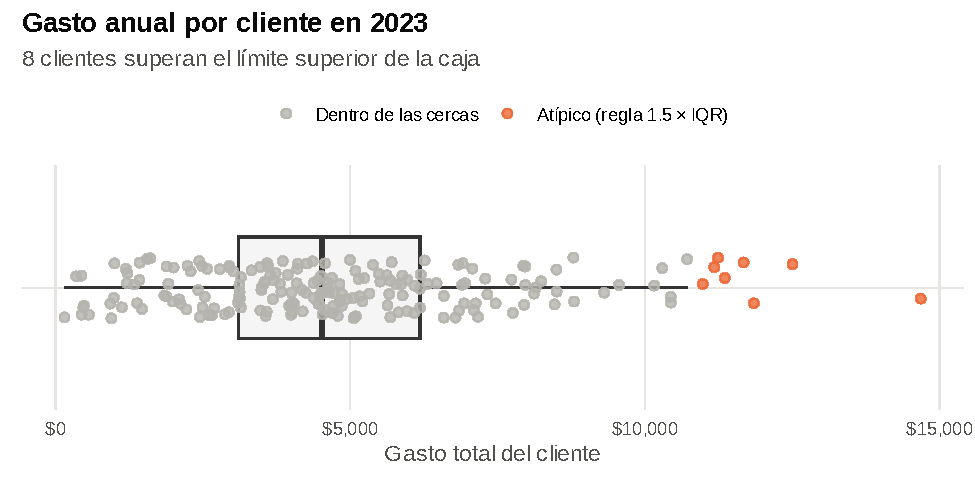
\includegraphics[width=0.9\textwidth]{m04-boxplot-clientes}
\caption{Diagrama de caja del gasto anual por cliente. Cada punto es un
cliente; en naranja, los que la regla del IQR marca como atípicos.}
\label{fig:m04-boxplot-clientes}
\end{figure}

En la figura~\ref{fig:m04-boxplot-clientes} la caja va del percentil 25 al 75,
la línea interior es la mediana y los ``bigotes'' llegan hasta el último dato
dentro de las cercas. Usamos \codigo{outlier.shape = NA} para que
\codigo{geom\_boxplot()} no dibuje sus propios puntos atípicos, porque ya los
dibujamos todos con \codigo{geom\_jitter()}.

\subsection{¿Qué hacer con un atípico?}

\begin{table}[H]
\centering
\small
\caption{Qué hacer con un dato atípico según su origen.}
\label{tab:m4-atipicos}
\begin{tabularx}{\textwidth}{@{}l X X@{}}
\toprule
\textbf{Situación} & \textbf{Acción} & \textbf{Ejemplo} \\
\midrule
Error de captura evidente & Corregir en la fuente si es posible; si no,
  excluir y documentarlo & 29,923.50 en lugar de 2,992.35 \\
Viola una regla de negocio & Separar y reportar al área responsable &
  Tickets negativos o en cero \\
Caso legítimo excepcional & Conservar; analizar aparte o usar medidas
  robustas (mediana, IQR) & Compra corporativa de 50 laptops \\
Cliente o producto de alto valor & Conservar y estudiar: suele ser una
  oportunidad & Los 8 clientes del ejemplo anterior \\
Posible fraude & Escalar a auditoría antes de tocarlo & Muchas devoluciones
  del mismo vendedor \\
\bottomrule
\end{tabularx}
\end{table}

\begin{advertencia}
Nunca borres atípicos ``porque estorban'' para que la gráfica se vea bonita
o el promedio salga mejor. Si decides excluir datos, deja constancia en tu
script (un comentario y un \codigo{filter()} explícito) y menciónalo en el
reporte: ``se excluyeron 3 registros con errores de captura''.
\end{advertencia}

\begin{hazlotu}
Carga \archivo{ventas\_retail.csv} y aplica \codigo{marcar\_atipicos()} a la
columna \codigo{total}. ¿Cuántas ventas quedan fuera de las cercas? Míralas
con \codigo{filter()}: ¿son errores o ventas grandes legítimas?
\end{hazlotu}

% ----------------------------------------------------------------------------
\section{KPIs y métricas de desempeño}
\label{sec:m4-kpis}

Un \termino{KPI} (\emph{Key Performance Indicator}, indicador clave de
desempeño) es una métrica que la empresa sigue de forma periódica para saber
si va bien o mal. Las ventas del mes son un dato; las ventas del mes
\emph{comparadas} contra el mes anterior, contra la meta o contra el mismo
mes del año pasado son un KPI. La tabla~\ref{tab:m4-kpis} resume los cálculos
más comunes.

\begin{table}[H]
\centering
\small
\caption{KPIs de desempeño más usados y su cálculo en R.}
\label{tab:m4-kpis}
\begin{tabularx}{\textwidth}{@{}l X l@{}}
\toprule
\textbf{KPI} & \textbf{Qué responde} & \textbf{Cálculo en R} \\
\midrule
Crecimiento MoM & ¿Cuánto crecimos contra el mes anterior?
  (\emph{Month over Month}) & \codigo{ventas / lag(ventas) - 1} \\
Acumulado (YTD) & ¿Cuánto llevamos vendido en el año?
  (\emph{Year to Date}) & \codigo{cumsum(ventas)} \\
Promedio móvil & ¿Cuál es la tendencia sin el ruido de cada mes? &
  \codigo{(v + lag(v) + lag(v, 2)) / 3} \\
Índice base 100 & ¿Cuánto cambiamos respecto a un punto de partida? &
  \codigo{ventas / first(ventas) * 100} \\
Variación vs meta & ¿Estamos arriba o abajo de lo planeado? &
  \codigo{ventas / meta - 1} \\
\bottomrule
\end{tabularx}
\end{table}

\begin{ejemplo}{Tablero mensual de ventas}
La meta comercial de 2023 era vender \$80,000 al mes. Construye una tabla
con las ventas mensuales, su crecimiento contra el mes anterior, el
acumulado del año, el promedio móvil de 3 meses, el índice con enero = 100 y
la variación contra la meta.
\end{ejemplo}

\begin{rcode}
meta_mensual <- 80000   # meta de ventas por mes

kpi_mensual <- transacciones %>%
  group_by(mes) %>%
  summarise(ventas = sum(total_transaccion), .groups = "drop") %>%
  arrange(mes) %>%                                  # orden cronológico
  mutate(
    crec_mom   = ventas / lag(ventas) - 1,          # vs mes anterior
    acumulado  = cumsum(ventas),                    # acumulado del año
    prom_movil = (ventas + lag(ventas) + lag(ventas, 2)) / 3,
    indice_100 = ventas / first(ventas) * 100,      # enero = 100
    vs_meta    = ventas / meta_mensual - 1          # sobre/bajo la meta
  )

kpi_mensual
\end{rcode}
\begin{rsalida}
# A tibble: 12 x 7
   mes     ventas crec_mom acumulado prom_movil indice_100  vs_meta
   <chr>    <dbl>    <dbl>     <dbl>      <dbl>      <dbl>    <dbl>
 1 2023-01 82560.  NA         82560.        NA       100    0.0320
 2 2023-02 65899.  -0.202    148459         NA        79.8 -0.176
 3 2023-03 90931.   0.380    239390.     79797.      110.   0.137
 4 2023-04 57038.  -0.373    296427.     71289.       69.1 -0.287
 5 2023-05 93910.   0.646    390338.     80626.      114.   0.174
 6 2023-06 88509.  -0.0575   478847.     79819.      107.   0.106
 7 2023-07 86456.  -0.0232   565303.     89625.      105.   0.0807
 8 2023-08 78929.  -0.0871   644232.     84632.       95.6 -0.0134
 9 2023-09 68856.  -0.128    713088.     78080.       83.4 -0.139
10 2023-10 70004.   0.0167   783092.     72596.       84.8 -0.125
11 2023-11 80507.   0.150    863599.     73122.       97.5  0.00634
12 2023-12 96394.   0.197    959993.     82302.      117.   0.205
\end{rsalida}

Cómo se lee cada columna, tomando marzo (\codigo{2023-03}) como ejemplo:
\begin{itemize}
  \item \codigo{crec\_mom} = 0.380: marzo vendió 38\% más que febrero.
  \item \codigo{acumulado} = 239,390: entre enero y marzo se vendieron
        \$239,390.
  \item \codigo{prom\_movil} = 79,797: el promedio de enero, febrero y marzo.
        Los dos primeros meses quedan en \codigo{NA} porque todavía no hay
        tres meses para promediar. La función \codigo{lag()} ``trae'' el
        valor de la fila anterior, y \codigo{lag(ventas, 2)} el de dos filas
        antes.
  \item \codigo{indice\_100} = 110: marzo vendió 10\% más que enero.
  \item \codigo{vs\_meta} = 0.137: marzo superó la meta en 13.7\%.
\end{itemize}

Para presentarla a la dirección conviene darle formato de negocio con las
funciones de \paquete{scales}:

\begin{rcode}
kpi_mensual %>%
  transmute(
    mes,
    ventas     = dollar(ventas, accuracy = 1),
    crec_mom   = percent(crec_mom, accuracy = 0.1),
    acumulado  = dollar(acumulado, accuracy = 1),
    vs_meta    = percent(vs_meta, accuracy = 0.1)
  )
\end{rcode}
\begin{rsalida}
# A tibble: 12 x 5
   mes     ventas  crec_mom acumulado vs_meta
   <chr>   <chr>   <chr>    <chr>     <chr>
 1 2023-01 $82,560 <NA>     $82,560   3.2%
 2 2023-02 $65,899 -20.2%   $148,459  -17.6%
 3 2023-03 $90,931 38.0%    $239,390  13.7%
 4 2023-04 $57,038 -37.3%   $296,427  -28.7%
 5 2023-05 $93,910 64.6%    $390,338  17.4%
 6 2023-06 $88,509 -5.8%    $478,847  10.6%
 7 2023-07 $86,456 -2.3%    $565,303  8.1%
 8 2023-08 $78,929 -8.7%    $644,232  -1.3%
 9 2023-09 $68,856 -12.8%   $713,088  -13.9%
10 2023-10 $70,004 1.7%     $783,092  -12.5%
11 2023-11 $80,507 15.0%    $863,599  0.6%
12 2023-12 $96,394 19.7%    $959,993  20.5%
\end{rsalida}

¿Qué nos dice el tablero? Los resultados mes a mes brincan mucho ($-20.2\%$,
$+38.0\%$, $-37.3\%$, $+64.6\%$\ldots). Abril (\$57,038) fue el peor mes,
28.7\% por debajo de la meta, y diciembre el mejor, 20.5\% por encima.
Contemos cuántos meses cumplieron la meta y cuánto faltó o sobró en el año:

\begin{rcode}
meses_arriba <- sum(kpi_mensual$vs_meta >= 0)   # meses que cumplieron
meses_arriba
sum(kpi_mensual$ventas) - meta_mensual * 12     # diferencia anual
\end{rcode}
\begin{rsalida}
[1] 7
[1] -7.31
\end{rsalida}

La meta mensual se cumplió en 7 de los 12 meses y el año cerró con \$959,993:
apenas \$7.31 por debajo de la meta anual de \$960,000. En el total anual la
empresa está en la meta, pero con un camino muy irregular. Para ver la
tendencia sin tanto ruido graficamos las ventas junto con su promedio móvil.

\begin{rcode}
# Formato largo: una fila por mes y por serie (Módulo 2, pivot_longer)
kpi_largo <- kpi_mensual %>%
  mutate(fecha_mes = as.Date(paste0(mes, "-01"))) %>%
  select(fecha_mes,
         `Ventas del mes` = ventas,
         `Promedio móvil 3 meses` = prom_movil) %>%
  pivot_longer(-fecha_mes, names_to = "serie", values_to = "valor")

p_kpi <- ggplot(kpi_largo, aes(x = fecha_mes, y = valor, color = serie)) +
  geom_hline(yintercept = meta_mensual, linetype = "dashed",
             color = "#52514e", linewidth = 0.5) +
  annotate("text", x = as.Date("2023-01-01"), y = meta_mensual + 2500,
           label = "Meta: $80,000", hjust = 0, size = 3.3,
           color = "#52514e") +
  geom_line(linewidth = 0.8, na.rm = TRUE) +
  geom_point(size = 1.8, na.rm = TRUE) +
  scale_color_manual(
    values = c("Ventas del mes" = color_principal,
               "Promedio móvil 3 meses" = color_resalte),
    breaks = c("Ventas del mes", "Promedio móvil 3 meses"),
    name = NULL) +
  scale_y_continuous(labels = dollar) +
  scale_x_date(date_breaks = "1 month", date_labels = "%b") +
  labs(title = "Ventas mensuales 2023 contra la meta",
       subtitle = "El promedio móvil suaviza los brincos de cada mes",
       x = NULL, y = "Ventas") +
  tema_libro()

p_kpi
\end{rcode}

\begin{figure}[H]
\centering
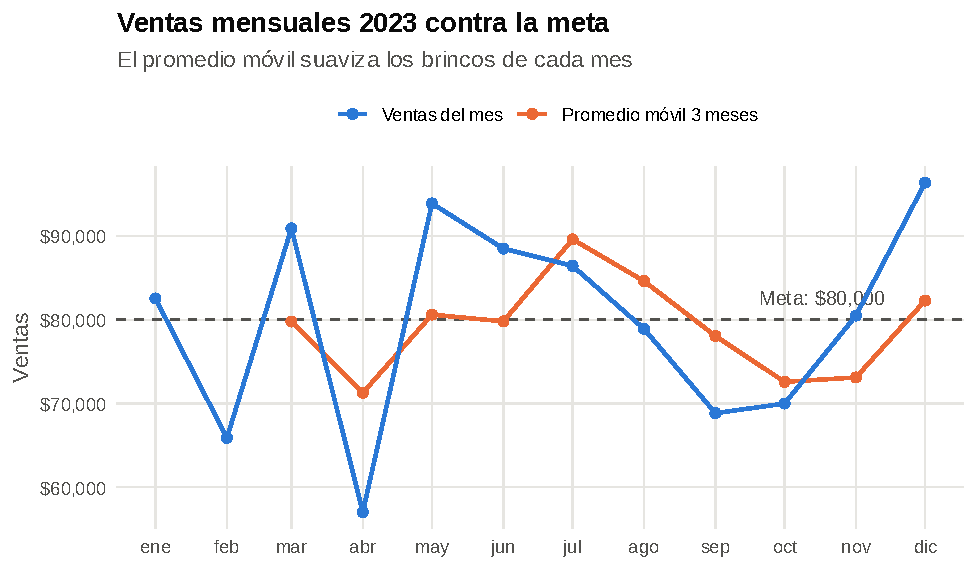
\includegraphics[width=0.9\textwidth]{m04-kpi-evolucion}
\caption{Ventas mensuales, promedio móvil de 3 meses y meta mensual.}
\label{fig:m04-kpi-evolucion}
\end{figure}

La figura~\ref{fig:m04-kpi-evolucion} cuenta la historia completa: las ventas
mensuales (azul) suben y bajan con fuerza, mientras que el promedio móvil
(naranja) muestra la tendencia de fondo: rondó la meta en primavera (con el
bache de abril), la superó en julio y agosto, cayó por debajo durante el
otoño y se recuperó en diciembre.

\begin{negocio}{Por qué los directivos piden promedios móviles}
Un mes malo aislado puede deberse a días festivos, a un problema de
inventario o simplemente al azar. Reaccionar a cada brinco (``abril cayó
37\%: ¡recorten gastos!'') lleva a decisiones erráticas. El promedio móvil
filtra ese ruido: si \emph{también} baja durante varios meses, entonces sí
hay una tendencia que atender. En empresas con estacionalidad fuerte se
complementa con el crecimiento contra el mismo mes del año anterior
(\emph{YoY}, \emph{Year over Year}).
\end{negocio}

\begin{consejo}
Para promedios móviles de muchos periodos (por ejemplo, 12 meses), escribir
\codigo{lag()} doce veces es incómodo. El paquete \paquete{zoo} (que se
instala junto con \paquete{forecast}) tiene
\codigo{zoo::rollmean(ventas, k = 12, fill = NA, align = "right")}, que hace
exactamente el mismo cálculo.
\end{consejo}

\begin{hazlotu}
Calcula los mismos KPIs por \codigo{trimestre} (crecimiento contra el
trimestre anterior, acumulado e índice base 100). ¿Qué trimestre fue el
mejor? ¿Cuál fue el crecimiento del cuarto trimestre contra el tercero?
\end{hazlotu}

% ----------------------------------------------------------------------------
\section{Análisis de Pareto y clasificación ABC}
\label{sec:m4-pareto}

El \termino{principio de Pareto}, o regla 80/20, dice que en muchos negocios
una minoría de elementos genera la mayoría de los resultados: el 20\% de los
productos genera el 80\% de las ventas, el 20\% de los clientes aporta el
80\% de los ingresos. Los porcentajes exactos varían; lo importante es la
idea de \emph{concentración}. El \termino{análisis ABC} aprovecha esa idea
para clasificar productos:

\begin{itemize}
  \item \textbf{Clase A}: los productos que, sumados de mayor a menor,
        acumulan el primer 80\% de los ingresos. Son vitales.
  \item \textbf{Clase B}: los que acumulan del 80\% al 95\%. Importantes.
  \item \textbf{Clase C}: el 5\% restante. Muchos productos que aportan poco.
\end{itemize}

\begin{ejemplo}{¿Qué productos sostienen el negocio?}
La directora quiere saber si hay un grupo pequeño de productos ``estrella''
del que dependa la empresa, para asegurarse de que nunca falten en
inventario.
\end{ejemplo}

\begin{rcode}
pareto <- transacciones %>%
  group_by(producto_id) %>%
  summarise(ingresos = sum(total_transaccion), .groups = "drop") %>%
  arrange(desc(ingresos)) %>%                        # de mayor a menor
  mutate(
    pct_ingresos  = ingresos / sum(ingresos),        # peso de cada uno
    pct_acumulado = cumsum(pct_ingresos),            # % acumulado
    pct_productos = row_number() / n(),              # % del catálogo
    clase = case_when(
      pct_acumulado <= 0.80 ~ "A",
      pct_acumulado <= 0.95 ~ "B",
      TRUE                  ~ "C"
    )
  ) %>%
  left_join(productos %>%
              select(producto_id, categoria, estado_stock, activo),
            by = "producto_id")

pareto %>%
  select(producto_id, ingresos, pct_ingresos, pct_acumulado, clase) %>%
  head(10)
\end{rcode}
\begin{rsalida}
# A tibble: 10 x 5
   producto_id ingresos pct_ingresos pct_acumulado clase
         <dbl>    <dbl>        <dbl>         <dbl> <chr>
 1           6   34028.       0.0354        0.0354 A
 2          19   28368.       0.0296        0.0650 A
 3          31   25430.       0.0265        0.0915 A
 4          47   24527.       0.0255        0.117  A
 5          46   24470.       0.0255        0.143  A
 6          32   24333.       0.0253        0.168  A
 7          14   24023.       0.0250        0.193  A
 8          24   23593.       0.0246        0.217  A
 9          29   22809.       0.0238        0.241  A
10          21   22083.       0.0230        0.264  A
\end{rsalida}

El producto más vendido (el 6) aporta apenas el 3.5\% de los ingresos, y los
10 primeros productos (el 20\% del catálogo) suman el 26.4\%. Muy lejos de
un 80/20. Veamos el resumen por clase:

\begin{rcode}
pareto %>%
  group_by(clase) %>%
  summarise(productos     = n(),
            pct_catalogo  = n() / nrow(pareto),
            ingresos      = sum(ingresos),
            pct_ingresos  = sum(pct_ingresos),
            .groups = "drop")
\end{rcode}
\begin{rsalida}
# A tibble: 3 x 5
  clase productos pct_catalogo ingresos pct_ingresos
  <chr>     <int>        <dbl>    <dbl>        <dbl>
1 A            36         0.72  764155.       0.796
2 B             9         0.18  137845.       0.144
3 C             5         0.1    57992.       0.0604
\end{rsalida}

\begin{rcode}
p_pareto <- ggplot(pareto, aes(x = pct_productos, y = pct_acumulado)) +
  # diagonal: lo que pasaría si todos los productos vendieran lo mismo
  geom_abline(slope = 1, intercept = 0, linetype = "dashed",
              color = color_gris) +
  geom_hline(yintercept = 0.80, color = "#52514e", linewidth = 0.4) +
  geom_line(color = "#52514e", linewidth = 0.6) +
  geom_point(aes(color = clase), size = 2) +
  # punto de referencia de la regla 80/20
  annotate("point", x = 0.2, y = 0.8, shape = 4, size = 4, stroke = 1.2) +
  annotate("text", x = 0.22, y = 0.86, hjust = 0, size = 3.3,
           label = "Regla 80/20 (referencia)") +
  scale_color_manual(values = paleta_libro[1:3], name = "Clase") +
  scale_x_continuous(labels = percent) +
  scale_y_continuous(labels = percent, limits = c(0, 1)) +
  labs(title = "Curva de Pareto de ingresos por producto",
       subtitle = "Ingresos muy repartidos: no hay pocos productos estrella",
       x = "% de productos (de mayor a menor ingreso)",
       y = "% acumulado de ingresos") +
  tema_libro()

p_pareto
\end{rcode}

\begin{figure}[H]
\centering
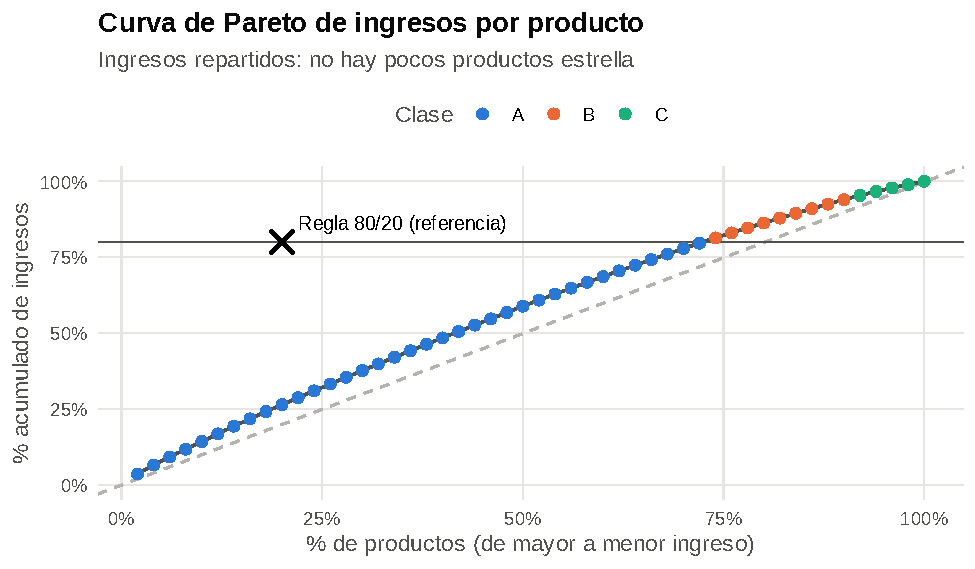
\includegraphics[width=0.9\textwidth]{m04-pareto}
\caption{Curva de Pareto. Cuanto más se despega la curva de la diagonal
punteada, más concentrados están los ingresos.}
\label{fig:m04-pareto}
\end{figure}

\begin{ejemplo}{Interpretar la curva de Pareto}
En la figura~\ref{fig:m04-pareto}, el eje horizontal es el porcentaje del
catálogo (ordenado de mayor a menor ingreso) y el vertical, el porcentaje
acumulado de ingresos. Si la empresa siguiera la regla 80/20, la curva
pasaría por la cruz. Nuestra curva está muy pegada a la diagonal: los 36
productos de la clase A (el 72\% del catálogo) apenas juntan el 79.6\% de los
ingresos. \textbf{Este es un hallazgo en sí mismo}: la empresa no depende de
unos cuantos productos estrella; sus ingresos están muy repartidos.
\end{ejemplo}

¿Qué implica para el inventario? Cruzamos la clase con el estado del stock:

\begin{rcode}
pareto %>% count(clase, estado_stock)

# Productos A con stock bajo: prioridad de reabastecimiento
pareto %>%
  filter(clase == "A", estado_stock != "Stock OK") %>%
  select(producto_id, categoria, ingresos, estado_stock)
\end{rcode}
\begin{rsalida}
# A tibble: 4 x 3
  clase estado_stock     n
  <chr> <chr>        <int>
1 A     Stock Bajo       4
2 A     Stock OK        32
3 B     Stock OK         9
4 C     Stock OK         5
# A tibble: 4 x 4
  producto_id categoria  ingresos estado_stock
        <dbl> <chr>         <dbl> <chr>
1           6 Juguetes     34028. Stock Bajo
2          33 Alimentos    21240. Stock Bajo
3           3 Automotriz   19908. Stock Bajo
4          39 Alimentos    18337. Stock Bajo
\end{rsalida}

\begin{negocio}{Políticas de inventario ABC}
\begin{itemize}
  \item \textbf{Clase A} (36 productos): revisión semanal de inventario,
        stock de seguridad alto y nunca permitir faltantes. Los 4 productos A
        con stock bajo (6, 33, 3 y 39) deben reabastecerse de inmediato;
        entre ellos está el producto 6, ¡el más vendido del año!
  \item \textbf{Clase B} (9 productos): revisión quincenal y stock de
        seguridad moderado.
  \item \textbf{Clase C} (5 productos): stock mínimo, pedidos bajo demanda y
        candidatos a revisión (¿se descontinúan?, ¿se promueven?).
\end{itemize}
Como nuestro catálogo es tan parejo, sacar productos C ahorraría poco espacio
pero tampoco perdería muchas ventas: 5 productos que suman el 6.0\% de los
ingresos. En catálogos reales, con miles de productos, la clase C suele
tener cientos de artículos que ocupan bodega y casi no se venden: ahí el ABC
libera mucho dinero.
\end{negocio}

\begin{hazlotu}
Haz el mismo análisis de Pareto con los \emph{clientes} en lugar de los
productos. ¿Qué porcentaje de clientes genera el 80\% de los ingresos? ¿Los
ingresos están más o menos concentrados que en los productos?
\end{hazlotu}

% ----------------------------------------------------------------------------
\section{Correlación: ¿qué variables se mueven juntas?}
\label{sec:m4-correlacion}

La \termino{correlación} mide qué tanto se mueven juntas dos variables
numéricas. Se resume en un número entre $-1$ y $+1$:
\begin{itemize}
  \item Cerca de $+1$: cuando una sube, la otra también sube (visitas a la
        tienda y ventas).
  \item Cerca de $-1$: cuando una sube, la otra baja (precio y unidades
        vendidas).
  \item Cerca de $0$: no hay relación \emph{lineal} (estatura del cliente y
        ticket).
\end{itemize}
Como guía práctica: $|r| < 0.3$ es una relación débil, entre $0.3$ y $0.7$
moderada, y mayor a $0.7$ fuerte.

\subsection{Pearson y Spearman}

La \termino{correlación de Pearson} ($r$) mide relaciones \emph{lineales}
(en línea recta) y usa los valores tal cual; por eso es sensible a los
atípicos. Su fórmula compara cómo se desvía cada variable de su media:
\[
  r = \frac{\sum (x_i - \bar{x})(y_i - \bar{y})}
           {\sqrt{\sum (x_i - \bar{x})^2}\,\sqrt{\sum (y_i - \bar{y})^2}}
\]
Si cuando $x$ está por encima de su media $y$ también lo está, los productos
del numerador son positivos y $r$ sale positiva. La \termino{correlación de
Spearman} ($\rho$, ``ro'') hace lo mismo pero con los \emph{lugares}
(rangos) que ocupa cada dato al ordenarlos; mide si la relación es
\emph{monótona} (siempre sube o siempre baja, aunque no sea en línea recta) y
casi no le afectan los atípicos.

\begin{ejemplo}{¿Qué explica el gasto de un cliente?}
Construimos una tabla con una fila por cliente: número de compras, unidades,
gasto total, ticket promedio, edad y antigüedad como cliente. Queremos saber
qué variables se relacionan con el gasto anual.
\end{ejemplo}

\begin{rcode}
perfil_clientes <- transacciones %>%
  group_by(cliente_id) %>%
  summarise(compras   = n(),
            unidades  = sum(cantidad),
            gasto     = sum(total_transaccion),
            ticket    = mean(total_transaccion),
            .groups = "drop") %>%
  left_join(clientes, by = "cliente_id") %>%
  mutate(antiguedad = as.numeric(as.Date("2023-12-31") - fecha_registro))

# Pearson (el método por defecto) y Spearman
cor(perfil_clientes$compras, perfil_clientes$gasto)
cor(perfil_clientes$compras, perfil_clientes$gasto, method = "spearman")
cor(perfil_clientes$edad, perfil_clientes$gasto)
\end{rcode}
\begin{rsalida}
[1] 0.7927073
[1] 0.7519843
[1] -0.07345163
\end{rsalida}

El número de compras tiene una correlación fuerte con el gasto (0.79 con
Pearson y 0.75 con Spearman): los clientes que más gastan son,
sobre todo, los que compran más veces. La edad, en cambio, casi no tiene
relación con el gasto ($-0.07$).

Para ver la diferencia entre ambos métodos, observa este ejemplo pequeño
creado a mano: diez tiendas donde las ventas suben siempre con el número de
visitantes, salvo que la décima tienda tuvo una venta corporativa enorme.

\begin{rcode}
visitantes <- c(100, 120, 150, 170, 200, 220, 250, 270, 300, 320)
ventas_dia <- c(10, 12, 14, 17, 19, 22, 24, 27, 29, 300)  # la última: atípica

cor(visitantes, ventas_dia)                        # Pearson
cor(visitantes, ventas_dia, method = "spearman")   # Spearman
\end{rcode}
\begin{rsalida}
[1] 0.5726456
[1] 1
\end{rsalida}

La relación es perfectamente monótona (más visitantes, siempre más ventas),
y Spearman lo detecta con $\rho = 1$. Pearson da 0.57 porque el dato
atípico rompe la línea recta. \textbf{Regla práctica}: usa Pearson cuando la
relación se vea lineal y no haya atípicos fuertes; usa Spearman con datos
asimétricos, con atípicos o con escalas ordinales (calificaciones de 1 a 5).

\subsection{Matriz de correlación}

Cuando tienes muchas variables, \codigo{cor()} aplicado a un data frame
numérico calcula todas las correlaciones a la vez: una
\termino{matriz de correlación}.

\begin{rcode}
matriz_cor <- perfil_clientes %>%
  select(compras, unidades, gasto, ticket, edad, antiguedad) %>%
  cor()

round(matriz_cor, 2)
\end{rcode}
\begin{rsalida}
           compras unidades gasto ticket  edad antiguedad
compras       1.00     0.91  0.79  -0.09 -0.02       0.01
unidades      0.91     1.00  0.87   0.14 -0.01       0.03
gasto         0.79     0.87  1.00   0.46 -0.07       0.05
ticket       -0.09     0.14  0.46   1.00 -0.14       0.05
edad         -0.02    -0.01 -0.07  -0.14  1.00       0.01
antiguedad    0.01     0.03  0.05   0.05  0.01       1.00
\end{rsalida}

La diagonal siempre vale 1 (cada variable consigo misma) y la matriz es
simétrica: la correlación de \codigo{compras} con \codigo{gasto} es la misma
que la de \codigo{gasto} con \codigo{compras}. Leer una tabla así es
cansado; \paquete{corrplot} la convierte en una imagen:

\begin{rcode}
corrplot(matriz_cor,
         method = "color",          # celdas coloreadas
         type = "upper",            # solo el triángulo superior
         addCoef.col = "black",     # escribe el coeficiente
         number.cex = 0.8,          # tamaño de los números
         tl.col = "black",          # color de los nombres
         tl.srt = 45,               # nombres inclinados
         col = colorRampPalette(c("#e34948", "white", "#2a78d6"))(200),
         diag = FALSE)              # sin la diagonal de unos
\end{rcode}

\begin{figure}[H]
\centering
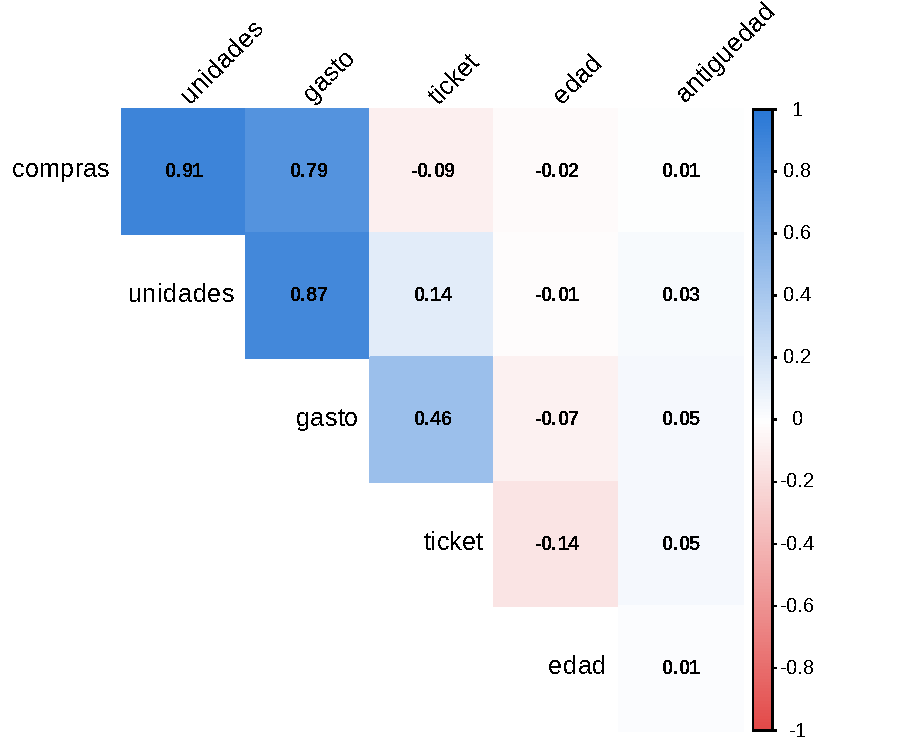
\includegraphics[width=0.75\textwidth]{m04-corrplot}
\caption{Matriz de correlación del perfil de clientes. Escala divergente:
azul = correlación positiva, rojo = negativa, blanco = sin relación.}
\label{fig:m04-corrplot}
\end{figure}

La figura~\ref{fig:m04-corrplot} usa una paleta \emph{divergente} (rojo,
blanco, azul) porque la correlación tiene un centro natural en cero. Se lee
de un vistazo: el gasto se explica por la frecuencia (\codigo{compras},
0.79) y por las \codigo{unidades} (0.87); el \codigo{ticket} promedio tiene
una relación moderada con el gasto (0.46), y la edad y la antigüedad no se
relacionan con nada. Para la directora esto significa que \textbf{aumentar la
frecuencia de compra} (que el cliente regrese) pesa más que la edad o la
antigüedad del cliente.

\subsection{¿La correlación es real? \texorpdfstring{\codigo{cor.test()}}{cor.test()}}

Una correlación calculada con pocos datos puede salir distinta de cero por
pura casualidad. La función \codigo{cor.test()} responde: \emph{si en
realidad no hubiera ninguna relación, ¿qué tan raro sería observar una
correlación como esta?} (en la sección~\ref{sec:m4-hipotesis} verás esta
lógica con detalle).

\begin{rcode}
cor.test(perfil_clientes$edad, perfil_clientes$gasto)
\end{rcode}
\begin{rsalida}
	Pearson's product-moment correlation

data:  perfil_clientes$edad and perfil_clientes$gasto
t = -1.0311, df = 196, p-value = 0.3038
alternative hypothesis: true correlation is not equal to 0
95 percent confidence interval:
 -0.21073472  0.06667273
sample estimates:
        cor
-0.07345163
\end{rsalida}

Lo que importa de esta salida:
\begin{itemize}
  \item \codigo{cor = -0.073}: la correlación de la muestra.
  \item \codigo{p-value = 0.3038}: una probabilidad de 30\%. Si la edad no
        tuviera ninguna relación con el gasto, sería muy común ver una
        correlación como esta solo por azar. Conclusión: \textbf{no hay
        evidencia} de que la edad se relacione con el gasto.
  \item \codigo{95 percent confidence interval}: el valor real de la
        correlación podría estar entre $-0.21$ y $0.07$; el intervalo
        incluye el cero.
\end{itemize}

\begin{hazlotu}
Aplica \codigo{cor.test()} a \codigo{compras} y \codigo{gasto}. ¿Qué
p-valor obtienes? ¿El intervalo de confianza incluye el cero? Repite con
\codigo{method = "spearman"}.
\end{hazlotu}

\subsection{Correlación no implica causalidad}
\label{sec:m4-causalidad}

Que dos variables se muevan juntas \textbf{no significa} que una cause a la
otra. Puede haber una tercera variable, llamada \termino{variable de
confusión}, que mueve a las dos. Para verlo con claridad \textbf{simulamos}
datos donde conocemos la verdad: en una cadena de tiendas, la temperatura
del día aumenta tanto la venta de helados como la de ventiladores, pero los
helados \emph{no} influyen en los ventiladores.

\begin{rcode}
set.seed(123)
dias_verano <- tibble(
  temperatura = runif(90, min = 18, max = 38),           # grados
  helados     = 20 + 3 * temperatura + rnorm(90, sd = 8),
  ventiladores = 5 + 1.5 * temperatura + rnorm(90, sd = 5)
)

# Ventas de helados vs ventiladores: correlación alta...
cor(dias_verano$helados, dias_verano$ventiladores)
\end{rcode}
\begin{rsalida}
[1] 0.8160674
\end{rsalida}

Una correlación de 0.82 es muy fuerte. Un análisis ingenuo diría: ``pongamos
los ventiladores junto a los helados, porque vender helados impulsa la venta
de ventiladores''. Pero sabemos (porque así los simulamos) que la única causa
común es la temperatura. En la sección~\ref{sec:m4-regresion} verás cómo la
regresión múltiple permite ``controlar'' por la temperatura y comprobar que,
a igual temperatura, los helados no explican los ventiladores.

\begin{negocio}{Correlaciones engañosas en la empresa}
\begin{itemize}
  \item ``Las tiendas con más empleados venden más'': tal vez las tiendas
        grandes tienen más empleados \emph{y} más clientes.
  \item ``Los clientes que usan la app gastan más'': quizá los clientes que
        ya gastaban mucho son los que descargan la app.
  \item ``Cuando subimos la publicidad subieron las ventas'': ¿o se subió la
        publicidad justo en diciembre, cuando las ventas suben solas?
\end{itemize}
Para demostrar causalidad se necesitan experimentos controlados (como las
pruebas A/B de la sección~\ref{sec:m4-ab}) o técnicas que controlen las
variables de confusión.
\end{negocio}

% ----------------------------------------------------------------------------
\section{Probabilidad y distribuciones útiles}
\label{sec:m4-probabilidad}

Una \termino{distribución de probabilidad} es un modelo que describe qué
valores puede tomar algo incierto y con qué probabilidad. No necesitas
memorizar fórmulas: R trae funciones con una convención de nombres muy
sencilla (tabla~\ref{tab:m4-distribuciones}).

\begin{table}[H]
\centering
\small
\caption{Prefijos de las funciones de distribución en R.}
\label{tab:m4-distribuciones}
\begin{tabularx}{\textwidth}{@{}l X l@{}}
\toprule
\textbf{Prefijo} & \textbf{Qué calcula} & \textbf{Ejemplos} \\
\midrule
\codigo{d} & Probabilidad de un valor exacto (densidad) & \codigo{dbinom()},
  \codigo{dpois()} \\
\codigo{p} & Probabilidad acumulada: $P(X \leq x)$ & \codigo{pnorm()},
  \codigo{pbinom()} \\
\codigo{q} & El valor que deja por debajo una probabilidad dada (cuantil) &
  \codigo{qnorm()} \\
\codigo{r} & Números aleatorios que siguen esa distribución & \codigo{rnorm()},
  \codigo{rbinom()} \\
\bottomrule
\end{tabularx}
\end{table}

\subsection{Distribución normal: ventas semanales}

La \termino{distribución normal} es la famosa ``campana de Gauss'':
simétrica, con la mayoría de los datos cerca de la media y cada vez menos
hacia los extremos. Queda definida por dos números: la media ($\mu$) y la
desviación estándar ($\sigma$). Una regla útil: en una normal, cerca del
68\% de los datos cae a menos de una desviación estándar de la media y el
95\% a menos de dos.

El ticket individual no es normal (tiene cola a la derecha), pero las
\emph{sumas} de muchas ventas tienden a serlo. Esto se debe al
\termino{teorema del límite central}, uno de los resultados más importantes
de la estadística: al sumar o promediar muchos datos independientes, el
resultado se parece cada vez más a una normal, sin importar la forma de los
datos originales. Comprobémoslo con las ventas semanales:

\begin{rcode}
ventas_semanales <- transacciones %>%
  # semanas completas de lunes a domingo (del 2 de enero al 31 de dic.)
  filter(fecha >= as.Date("2023-01-02")) %>%
  mutate(semana = floor_date(fecha, unit = "week", week_start = 1)) %>%
  group_by(semana) %>%
  summarise(ventas = sum(total_transaccion), .groups = "drop")

media_sem <- mean(ventas_semanales$ventas)
sd_sem    <- sd(ventas_semanales$ventas)
nrow(ventas_semanales)
c(media = media_sem, desv_est = sd_sem)
asimetria(ventas_semanales$ventas)
\end{rcode}
\begin{rsalida}
[1] 52
    media  desv_est
18444.936  4591.285
[1] 0.2219801
\end{rsalida}

Tenemos 52 semanas completas con venta media de \$18,445 y desviación
estándar de \$4,591. La asimetría es pequeña (0.22): la forma es casi
simétrica. La
figura~\ref{fig:m04-normal-semanal} compara el histograma con la curva
normal teórica.

\begin{rcode}
p_normal <- ggplot(ventas_semanales, aes(x = ventas)) +
  geom_histogram(aes(y = after_stat(density)), binwidth = 2000,
                 fill = color_principal, color = "white", alpha = 0.85) +
  # curva normal con la media y desviación de los datos
  stat_function(fun = dnorm, args = list(mean = media_sem, sd = sd_sem),
                color = color_resalte, linewidth = 0.9) +
  geom_vline(xintercept = 25000, linetype = "dashed", color = "#52514e") +
  annotate("text", x = 25300, y = 9e-05, hjust = 0, size = 3.3,
           label = "¿Más de $25,000?", color = "#52514e") +
  scale_x_continuous(labels = dollar) +
  scale_y_continuous(labels = NULL) +
  labs(title = "Ventas semanales de 2023 y curva normal",
       subtitle = "52 semanas; la curva naranja es Normal(18,445; 4,591)",
       x = "Ventas de la semana", y = "Densidad") +
  tema_libro()

p_normal
\end{rcode}

\begin{figure}[H]
\centering
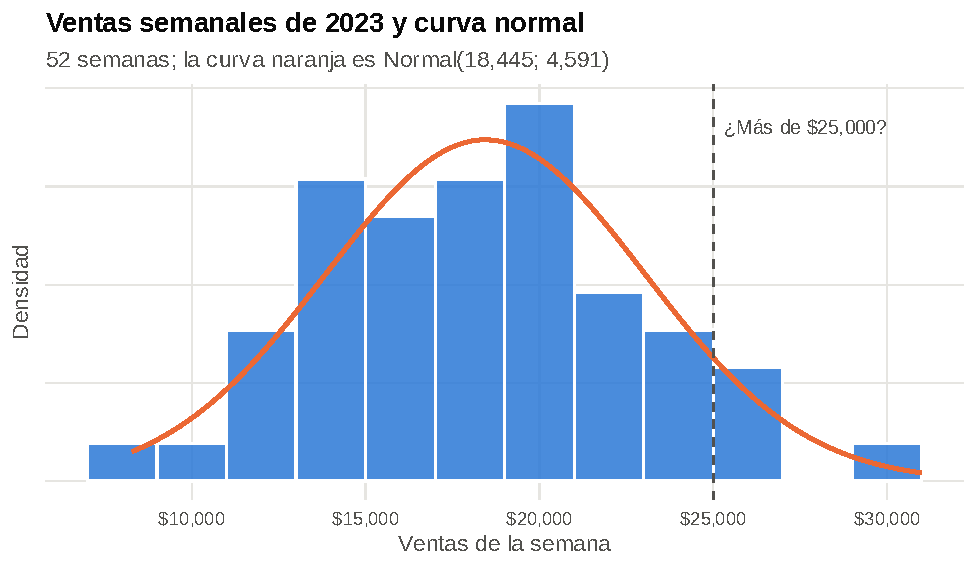
\includegraphics[width=0.9\textwidth]{m04-normal-semanal}
\caption{Las ventas semanales se ajustan bien a una distribución normal.}
\label{fig:m04-normal-semanal}
\end{figure}

Con el modelo normal podemos responder preguntas de planeación:

\begin{ejemplo}{Probabilidades con la normal}
\begin{enumerate}
  \item ¿Qué probabilidad hay de vender más de \$25,000 en una semana (lo
        que activaría un bono para el equipo)?
  \item ¿Cuánto inventario (en pesos) debe haber para cubrir la demanda del
        90\% de las semanas?
  \item ¿Qué probabilidad hay de una semana ``mala'', con menos de \$12,000?
\end{enumerate}
\end{ejemplo}

\begin{rcode}
# 1. P(ventas > 25,000) = 1 - P(ventas <= 25,000)
1 - pnorm(25000, mean = media_sem, sd = sd_sem)

# Comprobación con los datos reales: proporción de semanas > 25,000
mean(ventas_semanales$ventas > 25000)

# 2. Venta semanal que solo se supera el 10% de las veces
qnorm(0.90, mean = media_sem, sd = sd_sem)

# 3. P(ventas < 12,000)
pnorm(12000, mean = media_sem, sd = sd_sem)
\end{rcode}
\begin{rsalida}
[1] 0.0766864
[1] 0.07692308
[1] 24328.9
[1] 0.08019928
\end{rsalida}

Respuestas: (1) hay un 7.7\% de probabilidad de superar \$25,000 en una
semana, unas 4 semanas al año; los datos reales coinciden (7.7\%, es decir,
4 de 52 semanas). (2) Con un inventario equivalente a \$24,329 se cubre la
demanda del 90\% de las semanas. (3) Una semana por debajo de \$12,000 tiene
una probabilidad de 8.0\%.

\begin{advertencia}
Verifica siempre que la normal sea razonable antes de usarla (histograma,
asimetría cercana a cero). Si hubieras usado la normal con los
\emph{tickets individuales}, que tienen cola larga, habrías calculado
probabilidades negativas o muy equivocadas para los tickets bajos.
\end{advertencia}

\subsection{Distribución binomial: conversiones de una campaña}

La \termino{distribución binomial} cuenta cuántos ``éxitos'' hay en $n$
intentos independientes, cuando cada intento tiene la misma probabilidad
$p$ de éxito. Ejemplos: cuántos de 200 correos generan una compra, cuántos
de 50 clientes aceptan una oferta, cuántas de 1,000 piezas salen
defectuosas. El número esperado de éxitos es $n \times p$.

\begin{ejemplo}{Campaña de correo a clientes premium}
La empresa enviará un correo con una oferta a 200 clientes. Por campañas
anteriores, sabe que el 5\% de quienes reciben el correo compran. ¿Cuántas
compras debe esperar? ¿Qué probabilidad hay de conseguir exactamente 10?
¿Y de conseguir 15 o más, que es lo que el gerente prometió?
\end{ejemplo}

\begin{rcode}
n_correos  <- 200     # intentos
p_conv     <- 0.05    # probabilidad de conversión

n_correos * p_conv                            # conversiones esperadas
dbinom(10, size = n_correos, prob = p_conv)   # P(exactamente 10)
pbinom(5, size = n_correos, prob = p_conv)    # P(5 o menos)
1 - pbinom(14, size = n_correos, prob = p_conv)   # P(15 o más)
\end{rcode}
\begin{rsalida}
[1] 10
[1] 0.1283574
[1] 0.0623425
[1] 0.07813442
\end{rsalida}

Lo esperado son 10 compras, pero conseguir \emph{exactamente} 10 solo tiene
un 12.8\% de probabilidad: el azar mueve el resultado. Hay un 6.2\% de
probabilidad de un resultado decepcionante de 5 o menos, y apenas un 7.8\%
de llegar a 15 o más. El gerente prometió algo poco probable: para esperar
15 compras con un 5\% de conversión habría que enviar 300 correos.

\begin{rcode}
# ¿Cuántos correos hay que enviar para tener 90% de probabilidad
# de conseguir al menos 15 compras?
envios <- seq(200, 600, by = 10)
prob_15_o_mas <- 1 - pbinom(14, size = envios, prob = p_conv)
min(envios[prob_15_o_mas >= 0.90])
\end{rcode}
\begin{rsalida}
[1] 400
\end{rsalida}

Para prometer 15 compras con un 90\% de seguridad hay que enviar al menos 400
correos, el doble de lo planeado. Este tipo de cálculo evita compromisos
imposibles con la dirección.

\subsection{Distribución de Poisson: llegadas de clientes}

La \termino{distribución de Poisson} cuenta cuántos eventos ocurren en un
intervalo (de tiempo o de espacio) cuando ocurren al azar a un ritmo
promedio constante $\lambda$ (``lambda''). Ejemplos: clientes que llegan a
la caja por hora, llamadas al centro de atención por minuto, quejas por día.
Una propiedad característica: en una Poisson la media y la varianza son
iguales ($\lambda$).

Nuestros datos permiten comprobarlo. Contemos cuántas transacciones hubo
cada uno de los 365 días de 2023 (incluidos los días con cero ventas):

\begin{rcode}
tx_por_dia <- tibble(fecha = seq(as.Date("2023-01-01"),
                                 as.Date("2023-12-31"), by = "day")) %>%
  left_join(count(transacciones, fecha), by = "fecha") %>%
  mutate(n = replace_na(n, 0))              # días sin ventas = 0

lambda <- mean(tx_por_dia$n)
c(media = lambda, varianza = var(tx_por_dia$n))

# Frecuencia observada vs la que predice una Poisson(lambda)
tibble(transacciones_dia = 0:6) %>%
  mutate(
    dias_observados = map_int(transacciones_dia,
                              ~ sum(tx_por_dia$n == .x)),
    dias_poisson = round(365 * dpois(transacciones_dia, lambda), 1)
  )
\end{rcode}
\begin{rsalida}
   media varianza
2.739726 2.544709
# A tibble: 7 x 3
  transacciones_dia dias_observados dias_poisson
              <int>           <int>        <dbl>
1                 0              20         23.6
2                 1              69         64.6
3                 2              85         88.5
4                 3              78         80.8
5                 4              63         55.3
6                 5              32         30.3
7                 6              14         13.8
\end{rsalida}

La media (2.74) y la varianza (2.54) son muy parecidas, y los días
observados con 0, 1, 2\ldots{} transacciones se parecen mucho a los que
predice la Poisson. \codigo{map\_int()} (del paquete \paquete{purrr}, parte
del \paquete{tidyverse}) aplica el conteo a cada valor de
\codigo{transacciones\_dia}.

\begin{ejemplo}{Personal en cajas}
En la sucursal Centro llegan en promedio 12 clientes por hora a las cajas
en la tarde. Cada cajero atiende cómodamente a 8 clientes por hora. Con dos
cajeros (capacidad de 16), ¿qué probabilidad hay de que en una hora lleguen
más clientes de los que se pueden atender? ¿Y con tres cajeros
(capacidad 24)?
\end{ejemplo}

\begin{rcode}
lambda_hora <- 12
1 - ppois(16, lambda = lambda_hora)   # P(más de 16): 2 cajeros
1 - ppois(24, lambda = lambda_hora)   # P(más de 24): 3 cajeros
dpois(0, lambda = lambda_hora)        # P(ningún cliente en la hora)
\end{rcode}
\begin{rsalida}
[1] 0.101291
[1] 0.0006856332
[1] 6.144212e-06
\end{rsalida}

Con dos cajeros, en un 10.1\% de las horas de la tarde habrá más clientes
que capacidad (se formarán filas, aproximadamente 1 de cada 10 horas). Con
tres cajeros ese riesgo baja a 0.07\%. La última línea muestra que una hora
sin ningún cliente es prácticamente imposible (0.0006\%; el
\codigo{e-06} significa ``por $10^{-6}$''). La decisión ya no es ``intuición
contra intuición'': es comparar el costo de un tercer cajero contra el costo
de las filas en el 10\% de las horas.

\begin{hazlotu}
Si el ritmo sube a 15 clientes por hora en diciembre, ¿qué probabilidad hay
de superar la capacidad con dos cajeros? ¿Y con tres?
\end{hazlotu}

% ----------------------------------------------------------------------------
\section{Muestreo e intervalos de confianza}
\label{sec:m4-intervalos}

Casi nunca tienes todos los datos que te interesan. Los 1,000 tickets de
2023 son una \termino{muestra} de todas las compras que tus clientes harán;
una encuesta a 400 clientes es una muestra de toda la clientela (la
\termino{población}). La pregunta clave es: \emph{si tomara otra muestra,
¿cuánto cambiaría mi resultado?}

\subsection{Error estándar}

El \termino{error estándar} (EE) mide cuánto variaría la media si repitieras
el muestreo muchas veces. Se calcula así:
\[
  EE = \frac{s}{\sqrt{n}}
\]
Fíjate en el $\sqrt{n}$ del denominador: con más datos, el error estándar
baja, pero despacio. Para reducir el error a la mitad necesitas
\emph{cuatro} veces más datos.

\begin{rcode}
n_tickets <- length(ticket)
error_estandar <- sd(ticket) / sqrt(n_tickets)
error_estandar
\end{rcode}
\begin{rsalida}
[1] 24.0448
\end{rsalida}

No confundas los dos conceptos: la desviación estándar (\$760) dice cuánto
varían los tickets \emph{individuales}; el error estándar (\$24) dice cuánto
variaría el \emph{promedio} de 1,000 tickets.

\subsection{Intervalo de confianza para el ticket promedio}

Un \termino{intervalo de confianza} (IC) es un rango de valores plausibles
para el verdadero valor de la población. El IC del 95\% para una media se
construye como:
\[
  \bar{x} \;\pm\; t \times EE
\]
donde $t$ es un número que sale de la \termino{distribución t de Student}
(muy parecida a la normal) y, con muestras grandes, vale casi 2. Hagámoslo
``a mano'' y luego con \codigo{t.test()}:

\begin{rcode}
t_critico <- qt(0.975, df = n_tickets - 1)   # valor t para 95%
t_critico
media_ticket - t_critico * error_estandar    # límite inferior
media_ticket + t_critico * error_estandar    # límite superior

# Lo mismo en una línea:
t.test(ticket)$conf.int
\end{rcode}
\begin{rsalida}
[1] 1.962341
[1] 912.8086
[1] 1007.177
[1]  912.8086 1007.1768
attr(,"conf.level")
[1] 0.95
\end{rsalida}

\begin{concepto}{Cómo interpretar un intervalo de confianza}
Con los datos de 2023, el ticket promedio está entre \$912.81 y \$1,007.18
con una confianza del 95\%. La interpretación correcta es: \emph{si
repitiéramos este muestreo muchas veces y calculáramos un intervalo con cada
muestra, el 95\% de esos intervalos contendría el verdadero ticket
promedio}. En la práctica, dilo así: ``estimamos un ticket promedio de \$960,
con un margen de error de $\pm$\$47''.

\textbf{No es correcto} decir ``el 95\% de los tickets está entre \$913 y
\$1,007'': el intervalo habla del \emph{promedio}, no de los tickets
individuales (que van de \$23 a \$2,992).
\end{concepto}

\begin{negocio}{El margen de error en las decisiones}
Si el presupuesto de 2024 supone 12,000 transacciones, el ingreso esperado
es $12{,}000 \times 960 \approx$ 11.5 millones, pero con el IC podrías
presentar un rango: entre $12{,}000 \times 913 \approx$ 10.95 y
$12{,}000 \times 1{,}007 \approx$ 12.09 millones. Presentar un rango en
vez de un número único es más honesto y ayuda a planear escenarios.
\end{negocio}

\subsection{Bootstrap: intervalos sin fórmulas}

¿Y si quieres un intervalo para la \emph{mediana}, o para cualquier medida
que no tenga una fórmula sencilla? El \termino{bootstrap} es una técnica
ingeniosa: simula ``otras muestras'' tomando, con reemplazo, 1,000 tickets al
azar de tus propios 1,000 tickets. Algunos tickets saldrán repetidos y otros
no saldrán; así cada remuestra es ligeramente distinta. Repites esto miles de
veces, calculas la mediana de cada remuestra y te quedas con el 95\% central
de esos resultados.

\begin{rcode}
set.seed(123)   # para que el resultado sea reproducible
medianas_boot <- replicate(5000, {
  remuestra <- sample(ticket, size = length(ticket), replace = TRUE)
  median(remuestra)
})

length(medianas_boot)                           # 5,000 medianas
quantile(medianas_boot, probs = c(0.025, 0.975))   # IC 95% (percentiles)
\end{rcode}
\begin{rsalida}
[1] 5000
  2.5%  97.5%
641.23 796.43
\end{rsalida}

\codigo{replicate(5000, \{...\})} repite 5,000 veces el código entre llaves
y guarda cada resultado. El IC del 95\% para la mediana del ticket va de unos
\$641 a \$796. La figura~\ref{fig:m04-bootstrap} muestra las 5,000 medianas
simuladas.

\begin{rcode}
ic_boot <- quantile(medianas_boot, probs = c(0.025, 0.975))

p_boot <- ggplot(tibble(mediana = medianas_boot), aes(x = mediana)) +
  geom_histogram(binwidth = 5, fill = color_principal, color = "white") +
  geom_vline(xintercept = ic_boot, color = color_resalte,
             linewidth = 0.8, linetype = "dashed") +
  geom_vline(xintercept = mediana_ticket, color = "#0b0b0b",
             linewidth = 0.8) +
  scale_x_continuous(labels = dollar) +
  labs(title = "Distribución bootstrap de la mediana del ticket",
       subtitle = "5,000 remuestras; líneas naranjas = IC del 95%",
       x = "Mediana del ticket en cada remuestra",
       y = "Frecuencia") +
  tema_libro()

p_boot
\end{rcode}

\begin{figure}[H]
\centering
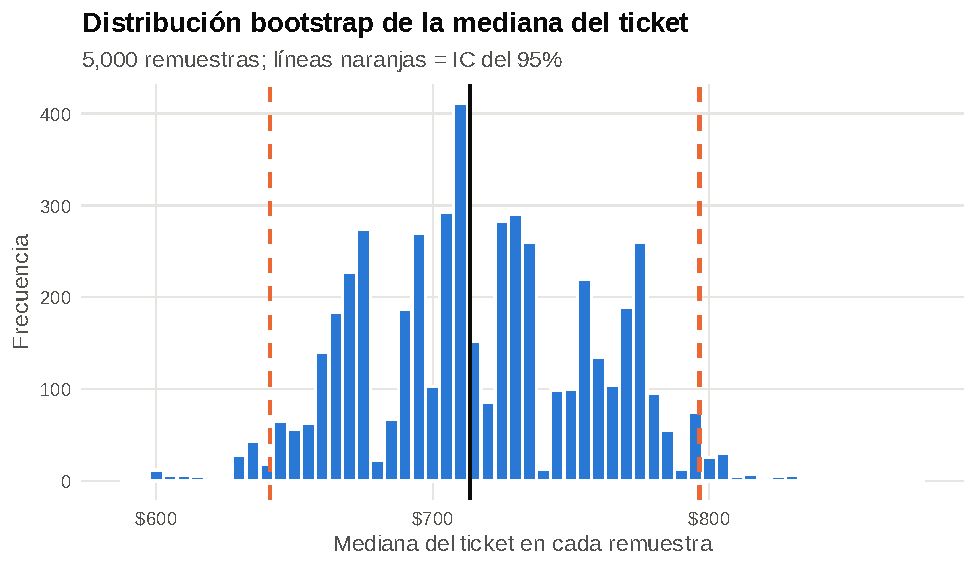
\includegraphics[width=0.9\textwidth]{m04-bootstrap}
\caption{Medianas de 5,000 remuestras bootstrap. La línea negra es la
mediana observada; entre las líneas naranjas queda el 95\% de las
remuestras.}
\label{fig:m04-bootstrap}
\end{figure}

\begin{hazlotu}
Usa el bootstrap para obtener un IC del 95\% del \emph{percentil 90} del
ticket (cambia \codigo{median(remuestra)} por
\codigo{quantile(remuestra, 0.9)}). ¿Es más ancho o más angosto que el de la
mediana? ¿Por qué crees que pasa?
\end{hazlotu}

% ----------------------------------------------------------------------------
\section{Pruebas de hipótesis para negocios}
\label{sec:m4-hipotesis}

Llegamos a la pregunta que aparece en todas las juntas: \emph{``¿esta
diferencia es real o es casualidad?''}. Los clientes premium gastan en
promedio \$977 por ticket y los demás \$951. ¿Es suficiente para decir que
los premium gastan más? Con otra muestra de tickets, la diferencia podría
desaparecer o invertirse. Las \termino{pruebas de hipótesis} dan un método
para decidir.

\subsection{La lógica en cinco conceptos}

\begin{concepto}{Hipótesis nula, alternativa y p-valor}
\begin{itemize}
  \item \termino{Hipótesis nula} ($H_0$): la postura ``aburrida'': no hay
        diferencia, no hay efecto. Ejemplo: ``el ticket promedio de premium y
        no premium es igual''.
  \item \termino{Hipótesis alternativa} ($H_1$): lo que quieres demostrar:
        ``el ticket promedio es distinto''.
  \item \termino{p-valor}: la probabilidad de observar una diferencia
        \emph{tan grande o más} que la de tus datos \textbf{si $H_0$ fuera
        cierta}. Un p-valor pequeño significa: ``sería muy raro ver esto por
        puro azar''.
  \item \termino{Nivel de significancia} ($\alpha$): el umbral que fijas
        \emph{antes} de ver los datos, casi siempre 0.05 (5\%). Si
        $p < \alpha$ rechazas $H_0$ y dices que el resultado es
        \termino{estadísticamente significativo}. Si $p \geq \alpha$,
        \emph{no} rechazas $H_0$: no hay evidencia suficiente.
\end{itemize}
\end{concepto}

Una analogía útil es un juicio: $H_0$ es ``el acusado es inocente''. Solo lo
declaras culpable si la evidencia es muy fuerte (p-valor pequeño). Si la
evidencia no alcanza, el veredicto es ``no culpable'', que \textbf{no es lo
mismo} que ``inocente demostrado''. Igual en estadística: no rechazar $H_0$
no demuestra que no haya diferencia; solo dice que tus datos no la
demuestran.

\begin{table}[H]
\centering
\small
\caption{Los dos errores posibles en una prueba de hipótesis.}
\label{tab:m4-errores}
\begin{tabularx}{\textwidth}{@{}l X X@{}}
\toprule
 & \textbf{En realidad $H_0$ es cierta} & \textbf{En realidad $H_0$ es falsa} \\
\midrule
\textbf{Rechazas $H_0$} & \termino{Error tipo I} (falso positivo): lanzas a
  todo el país una campaña que en realidad no funciona. Su probabilidad es
  $\alpha$. & Acierto: detectas un efecto real. \\
\textbf{No rechazas $H_0$} & Acierto: no te dejas engañar por el azar. &
  \termino{Error tipo II} (falso negativo): descartas una campaña que sí
  funcionaba. Se reduce con muestras más grandes. \\
\bottomrule
\end{tabularx}
\end{table}

\begin{advertencia}
\textbf{Significancia estadística no es lo mismo que importancia práctica.}
Con millones de datos, una diferencia de 50 centavos en el ticket puede ser
``significativa'' ($p < 0.05$) y aun así no importarle a nadie. Con pocos
datos, una diferencia enorme puede no ser significativa. Reporta siempre el
\emph{tamaño} de la diferencia (en pesos o en puntos porcentuales) junto con
el p-valor, y pregúntate: ¿esta diferencia cambia alguna decisión?
\end{advertencia}

\subsection{Prueba t: ¿los clientes premium gastan más?}

La \termino{prueba t de Student} compara las medias de dos grupos. Primero
unimos las transacciones con los clientes (Módulo~\ref{cap:manipulacion})
para saber quién es premium:

\begin{rcode}
tx_clientes <- transacciones %>%
  left_join(clientes, by = "cliente_id")

tx_clientes %>%
  group_by(es_premium) %>%
  summarise(tickets = n(),
            media   = mean(total_transaccion),
            mediana = median(total_transaccion),
            desv    = sd(total_transaccion),
            .groups = "drop")
\end{rcode}
\begin{rsalida}
# A tibble: 2 x 5
  es_premium tickets media mediana  desv
  <lgl>        <int> <dbl>   <dbl> <dbl>
1 FALSE          653  951.    672.  775.
2 TRUE           347  977.    803.  732.
\end{rsalida}

Planteamos: $H_0$: el ticket promedio es igual en ambos grupos;
$H_1$: es distinto. Nivel de significancia $\alpha = 0.05$.

\begin{rcode}
prueba_premium <- t.test(total_transaccion ~ es_premium,
                         data = tx_clientes)
prueba_premium
\end{rcode}
\begin{rsalida}
	Welch Two Sample t-test

data:  total_transaccion by es_premium
t = -0.52255, df = 741.31, p-value = 0.6014
alternative hypothesis: true difference in means between group FALSE and group TRUE is not equal to 0
95 percent confidence interval:
 -123.43528   71.53793
sample estimates:
mean in group FALSE  mean in group TRUE
           950.9885            976.9372
\end{rsalida}

Lectura línea por línea:
\begin{itemize}
  \item \codigo{Welch Two Sample t-test}: R usa por defecto la versión de
        Welch, que no supone que los dos grupos tengan la misma varianza. Es
        la opción segura.
  \item \codigo{t = -0.52255}: el \termino{estadístico t}, la diferencia de
        medias medida en errores estándar. Valores lejos de cero (más allá de
        $\pm 2$, aproximadamente) indican diferencias claras; $-0.52$ está
        muy cerca de cero.
  \item \codigo{p-value = 0.6014}: si premium y no premium gastaran lo mismo,
        veríamos una diferencia como esta el 60\% de las veces. Como
        $0.60 > 0.05$, \textbf{no rechazamos $H_0$}.
  \item \codigo{95 percent confidence interval}: la diferencia real
        (no premium menos premium) está entre $-123$ y $+72$ pesos. Incluye
        el cero.
  \item \codigo{sample estimates}: las medias de cada grupo.
\end{itemize}

Puedes extraer las piezas para usarlas en un reporte:

\begin{rcode}
prueba_premium$p.value
prueba_premium$conf.int
\end{rcode}
\begin{rsalida}
[1] 0.6014434
[1] -123.43528   71.53793
attr(,"conf.level")
[1] 0.95
\end{rsalida}

\begin{negocio}{``No hay evidencia'' es un resultado valioso}
Conclusión para la directora: \emph{con los datos de 2023 no hay evidencia
de que los clientes premium tengan un ticket promedio distinto al de los
demás; la diferencia observada (\$26) es compatible con el azar}. Esto no es
un fracaso del análisis: es información para decidir. Si la membresía premium
cuesta dinero (descuentos, envíos gratis), hay que preguntarse qué obtiene
la empresa a cambio. Quizá los premium compran con más \emph{frecuencia}
aunque no gasten más por ticket: esa es la siguiente hipótesis a revisar
(ejercicio~\ref{ej:m4-6}).
\end{negocio}

\subsection{Prueba A/B de proporciones: campaña A vs campaña B}
\label{sec:m4-ab}

Una \termino{prueba A/B} es un experimento: divides al azar a tus clientes en
dos grupos, a cada uno le muestras una versión distinta (de un correo, una
página, un precio) y comparas los resultados. Como la asignación es al azar,
las dos poblaciones son iguales en todo lo demás, y la diferencia se puede
atribuir a la versión. Es la forma más limpia de demostrar
\emph{causalidad} en un negocio.

\begin{ejemplo}{¿Qué asunto de correo convierte más?}
Mercadotecnia envió 2,000 correos con el asunto A (``Ofertas de la
semana'') y 2,000 con el asunto B (``Tu cupón personal te espera''). Como
queremos saber si el método funciona, \textbf{simulamos} los resultados con
tasas de conversión conocidas: 5\% para A y 6.5\% para B. En la vida real no
conocerías estas tasas: justamente eso es lo que la prueba intenta
averiguar.
\end{ejemplo}

\begin{rcode}
set.seed(123)
campana <- tibble(
  version  = rep(c("A", "B"), each = 2000),
  # 1 = compró, 0 = no compró; tasas reales: A 5%, B 6.5%
  convirtio = c(rbinom(2000, size = 1, prob = 0.050),
                rbinom(2000, size = 1, prob = 0.065))
)

resumen_ab <- campana %>%
  group_by(version) %>%
  summarise(enviados    = n(),
            conversiones = sum(convirtio),
            tasa        = mean(convirtio),
            .groups = "drop")
resumen_ab
\end{rcode}
\begin{rsalida}
# A tibble: 2 x 4
  version enviados conversiones   tasa
  <chr>      <int>        <int>  <dbl>
1 A           2000          101 0.0505
2 B           2000          130 0.065
\end{rsalida}

$H_0$: las dos versiones tienen la misma tasa de conversión. $H_1$: las tasas
son distintas. La función \codigo{prop.test()} recibe el número de éxitos y
el número de intentos de cada grupo:

\begin{rcode}
prueba_ab <- prop.test(x = resumen_ab$conversiones,
                       n = resumen_ab$enviados)
prueba_ab
\end{rcode}
\begin{rsalida}
	2-sample test for equality of proportions with continuity
	correction

data:  resumen_ab$conversiones out of resumen_ab$enviados
X-squared = 3.602, df = 1, p-value = 0.05771
alternative hypothesis: two.sided
95 percent confidence interval:
 -0.0294509801  0.0004509801
sample estimates:
prop 1 prop 2
0.0505 0.0650
\end{rsalida}

Lectura: la versión A convirtió 5.05\% y la B 6.50\%, pero el p-valor es
0.058, apenas \emph{mayor} a 0.05. Formalmente \textbf{no rechazamos $H_0$}:
con 2,000 correos por grupo, una diferencia así todavía podría deberse al
azar. El intervalo de confianza de la diferencia (A menos B) va de $-2.9$ a
$+0.05$ puntos porcentuales e incluye el cero.

Aquí hay una lección importante. Nosotros \emph{sabemos} que B es mejor
(así lo simulamos), y aun así la prueba no lo detectó: acabamos de cometer
un \textbf{error tipo II}. ¿La causa? Una muestra demasiado pequeña para
detectar una diferencia de 1.5 puntos. La función \codigo{power.prop.test()}
calcula cuántos envíos se necesitan para detectar una diferencia con una
probabilidad dada (la \termino{potencia}, típicamente 80\%):

\begin{rcode}
power.prop.test(p1 = 0.05, p2 = 0.065, power = 0.80)$n
\end{rcode}
\begin{rsalida}
[1] 3779.801
\end{rsalida}

Se necesitan unos 3,780 correos \emph{por grupo}. Repetimos el experimento
(de nuevo simulado, con las mismas tasas reales) con 4,000 correos por
versión:

\begin{rcode}
set.seed(123)
campana_4000 <- tibble(
  version   = rep(c("A", "B"), each = 4000),
  convirtio = c(rbinom(4000, size = 1, prob = 0.050),
                rbinom(4000, size = 1, prob = 0.065))
)

resumen_4000 <- campana_4000 %>%
  group_by(version) %>%
  summarise(enviados = n(), conversiones = sum(convirtio),
            .groups = "drop")

prop.test(x = resumen_4000$conversiones, n = resumen_4000$enviados)
\end{rcode}
\begin{rsalida}
	2-sample test for equality of proportions with continuity
	correction

data:  resumen_4000$conversiones out of resumen_4000$enviados
X-squared = 5.0351, df = 1, p-value = 0.02484
alternative hypothesis: two.sided
95 percent confidence interval:
 -0.022041478 -0.001458522
sample estimates:
 prop 1  prop 2
0.04975 0.06150
\end{rsalida}

Ahora $p = 0.025 < 0.05$: rechazamos $H_0$ y concluimos que el asunto B
convierte más (6.15\% contra 4.98\%). El intervalo (que R calcula como A menos B,
por eso sale negativo) dice que B supera a A por entre 0.15 y 2.2 puntos
porcentuales. Y la \emph{significancia práctica} es
clara: un punto más de conversión sobre 100,000 correos son unas 1,000
compras adicionales.

\begin{consejo}
Decide el tamaño de la prueba A/B \emph{antes} de lanzarla (con
\codigo{power.prop.test()}) y no la detengas en cuanto el p-valor baje de
0.05: si revisas el resultado cada hora y paras cuando ``sale'', aumentas
mucho la probabilidad de un falso positivo (error tipo I).
\end{consejo}

\subsection{ANOVA: ¿el ticket cambia entre categorías?}

Cuando quieres comparar las medias de \emph{más de dos} grupos, no hagas
muchas pruebas t de dos en dos (con 10 categorías serían 45 pruebas, y
alguna saldría ``significativa'' por azar). Usa el \termino{análisis de
varianza} (ANOVA). $H_0$: todas las medias son iguales; $H_1$: al menos una
es distinta. La idea es comparar cuánto varían las medias \emph{entre}
grupos con cuánto varían los datos \emph{dentro} de cada grupo.

\begin{rcode}
tx_productos <- transacciones %>%
  left_join(productos, by = "producto_id")

ticket_categoria <- tx_productos %>%
  group_by(categoria) %>%
  summarise(n     = n(),
            media = mean(total_transaccion),
            ee    = sd(total_transaccion) / sqrt(n()),
            .groups = "drop") %>%
  arrange(desc(media))
ticket_categoria
\end{rcode}
\begin{rsalida}
# A tibble: 10 x 4
   categoria       n media    ee
   <chr>       <int> <dbl> <dbl>
 1 Juguetes      118 1060.  77.1
 2 Alimentos     115 1057.  69.9
 3 Automotriz    105  991.  76.5
 4 Hogar          64  991.  90.7
 5 Belleza       187  974.  58.8
 6 Electrónica   137  968.  61.7
 7 Deportes       92  937.  78.3
 8 Libros         70  817.  85.2
 9 Ropa           38  791. 127.
10 Mascotas       74  779.  70.5
\end{rsalida}

Los tickets promedio van de \$779 (Mascotas) a \$1,060 (Juguetes). ¿Es una
diferencia real? Veamos las medias con su intervalo de confianza
aproximado (media $\pm$ 2 errores estándar):

\begin{rcode}
p_anova <- ggplot(ticket_categoria,
                  aes(x = media, y = reorder(categoria, media))) +
  geom_vline(xintercept = mean(ticket), linetype = "dashed",
             color = color_gris) +
  geom_errorbarh(aes(xmin = media - 2 * ee, xmax = media + 2 * ee),
                 height = 0.25, color = color_principal,
                 linewidth = 0.8) +
  geom_point(size = 2.5, color = color_principal) +
  scale_x_continuous(labels = dollar) +
  labs(title = "Ticket promedio por categoría con IC del 95%",
       subtitle = "Los intervalos se enciman mucho; línea gris = promedio general",
       x = "Ticket promedio", y = NULL) +
  tema_libro()

p_anova
\end{rcode}

\begin{figure}[H]
\centering
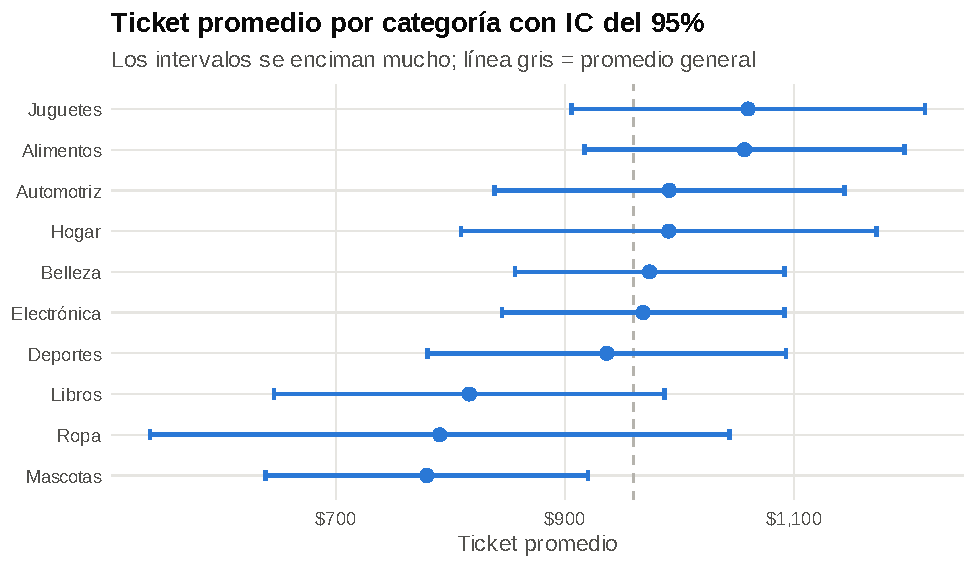
\includegraphics[width=0.9\textwidth]{m04-anova-categorias}
\caption{Ticket promedio por categoría. Cuando los intervalos se enciman
tanto, es difícil afirmar que alguna categoría sea distinta.}
\label{fig:m04-anova-categorias}
\end{figure}

\begin{rcode}
modelo_anova <- aov(total_transaccion ~ categoria, data = tx_productos)
summary(modelo_anova)
\end{rcode}
\begin{rsalida}
             Df    Sum Sq Mean Sq F value Pr(>F)
categoria     9   7466897  829655   1.441  0.166
Residuals   990 570107428  575866
\end{rsalida}

La columna clave es \codigo{Pr(>F)}, el p-valor: 0.166. Como es mayor a
0.05, \textbf{no hay evidencia} de que el ticket promedio dependa de la
categoría. El \codigo{F value} (1.441) compara la variación entre categorías
con la variación dentro de ellas; valores cercanos a 1 indican que las
categorías no se distinguen más de lo que se distinguen los tickets entre
sí. Hallazgo para la directora: las categorías difieren en \emph{volumen}
(Belleza tiene 187 tickets y Ropa 38), no en ticket promedio.

\subsubsection{Cuando el ANOVA sí es significativo: TukeyHSD}

Probemos ahora con el segmento de edad del cliente (Joven, Adulto, Maduro,
Senior):

\begin{rcode}
modelo_segmento <- aov(total_transaccion ~ segmento, data = tx_clientes)
summary(modelo_segmento)
\end{rcode}
\begin{rsalida}
             Df    Sum Sq Mean Sq F value Pr(>F)
segmento      3   4672766 1557589   2.708 0.0441 *
Residuals   996 572901558  575202
---
...
\end{rsalida}

Ahora $p = 0.044 < 0.05$: al menos un segmento tiene un ticket promedio
distinto. El asterisco junto al p-valor es la forma en que R marca la
significancia (una estrella: $p < 0.05$; dos: $p < 0.01$; tres:
$p < 0.001$); la leyenda completa aparece en la línea
\codigo{Signif. codes}, que aquí recortamos. ¿Cuál? El ANOVA no lo dice. Para eso se usa la prueba de
\termino{Tukey HSD} (\emph{Honest Significant Difference}), que compara
todos los pares de grupos ajustando los p-valores por hacer varias
comparaciones:

\begin{rcode}
TukeyHSD(modelo_segmento)
\end{rcode}
\begin{rsalida}
  Tukey multiple comparisons of means
    95% family-wise confidence level

Fit: aov(formula = total_transaccion ~ segmento, data = tx_clientes)

$segmento
                    diff        lwr       upr     p adj
Joven-Adulto    62.47256 -170.39680 295.34191 0.9007953
Maduro-Adulto -138.85507 -299.46454  21.75439 0.1172294
Senior-Adulto  -47.79558 -216.73288 121.14173 0.8858662
Maduro-Joven  -201.32763 -423.37427  20.71901 0.0912671
Senior-Joven  -110.26813 -338.41089 117.87463 0.5990701
Senior-Maduro   91.05950  -62.61673 244.73573 0.4229310
\end{rsalida}

Cada fila es una comparación: \codigo{diff} es la diferencia de medias,
\codigo{lwr} y \codigo{upr} su intervalo de confianza y \codigo{p adj} el
p-valor ajustado. Ningún par individual queda por debajo de 0.05; el más
cercano es Maduro contra Joven ($p = 0.09$): los clientes maduros gastan unos
\$201 menos por ticket que los jóvenes. Esto pasa a veces: el ANOVA detecta
que ``algo'' difiere, pero la evidencia es débil y no alcanza para señalar
un par concreto. \textbf{Conclusión honesta}: hay indicios de que el ticket
varía con la edad (los maduros gastan algo menos), pero la evidencia es
débil; conviene confirmarlo con los datos de 2024 antes de diseñar una
campaña por edad.

\subsection{Chi-cuadrada: ¿el método de pago depende de la tienda?}

Las pruebas anteriores comparan \emph{promedios} de una variable numérica.
Cuando las dos variables son \emph{categóricas}, se usa la \termino{prueba
chi-cuadrada de independencia} ($\chi^2$). $H_0$: las dos variables son
independientes (la mezcla de métodos de pago es la misma en todas las
tiendas); $H_1$: están relacionadas.

\begin{ejemplo}{Terminales de pago por sucursal}
Finanzas quiere saber si debe negociar terminales bancarias distintas para
cada sucursal o si todas las tiendas tienen la misma mezcla de métodos de
pago.
\end{ejemplo}

\begin{rcode}
tabla_pago <- table(transacciones$metodo_pago, transacciones$tienda_id)
tabla_pago
\end{rcode}
\begin{rsalida}
                   1  2  3  4  5  6  7  8  9 10
  Efectivo        26 36 35 29 33 43 28 31 27 27
  Tarjeta Crédito 37 37 35 29 38 28 32 29 45 40
  Tarjeta Débito  14 19 28 25 15 30 16 33 25 28
  Transferencia   10  7 11 11  9  8  9 13 11 13
\end{rsalida}

\begin{rcode}
prueba_chi <- chisq.test(tabla_pago)
prueba_chi
round(prueba_chi$expected[, 1:5], 1)   # conteos esperados (5 tiendas)
\end{rcode}
\begin{rsalida}
	Pearson's Chi-squared test

data:  tabla_pago
X-squared = 28.953, df = 27, p-value = 0.3632


                     1    2    3    4    5
  Efectivo        27.4 31.2 34.3 29.6 29.9
  Tarjeta Crédito 30.4 34.6 38.1 32.9 33.2
  Tarjeta Débito  20.3 23.1 25.4 21.9 22.1
  Transferencia    8.9 10.1 11.1  9.6  9.7
\end{rsalida}

El p-valor es 0.36: \textbf{no hay evidencia} de que el método de pago
dependa de la tienda. Las diferencias que ves en la tabla (por ejemplo, 13
transferencias en la tienda 8 contra 7 en la tienda 2) son las esperables
por azar. Los \codigo{expected} son los conteos que habría si las variables
fueran totalmente independientes; la prueba compara los observados con
estos. Decisión práctica: una sola negociación con el banco, con la misma
configuración de terminales para todas las sucursales.

\begin{advertencia}
La chi-cuadrada necesita conteos esperados de al menos 5 en casi todas las
celdas. Si hay muchas celdas con esperados pequeños, R muestra la advertencia
\codigo{Chi-squared approximation may be incorrect}. En ese caso agrupa
categorías poco frecuentes o usa \codigo{fisher.test()}.
\end{advertencia}

\subsection{¿Qué prueba uso?}

\begin{table}[H]
\centering
\small
\caption{Guía rápida para elegir una prueba de hipótesis.}
\label{tab:m4-que-prueba}
\begin{tabularx}{\textwidth}{@{}X X l@{}}
\toprule
\textbf{Pregunta de negocio} & \textbf{Tipo de datos} & \textbf{Función} \\
\midrule
¿El ticket promedio es distinto de \$900? & Una variable numérica vs un
  valor & \codigo{t.test(x, mu = 900)} \\
¿Premium y no premium gastan distinto? & Numérica + categórica de 2 grupos
  & \codigo{t.test(y \textasciitilde{} g)} \\
¿Mejoró la venta de cada tienda después del cambio? & Numérica, mismos
  sujetos antes y después & \codigo{t.test(antes, despues, paired = TRUE)} \\
¿Qué versión de la campaña convierte más? & Proporciones de 2 o más grupos &
  \codigo{prop.test()} \\
¿El ticket cambia entre categorías o tiendas? & Numérica + categórica de 3
  o más grupos & \codigo{aov()} + \codigo{TukeyHSD()} \\
¿El método de pago depende de la tienda? & Dos variables categóricas &
  \codigo{chisq.test()} \\
¿El gasto se relaciona con la edad? & Dos numéricas & \codigo{cor.test()} \\
Datos muy asimétricos o pocos datos (alternativa sin supuesto de
  normalidad) & Numérica + 2 grupos / 3+ grupos &
  \codigo{wilcox.test()} / \codigo{kruskal.test()} \\
\bottomrule
\end{tabularx}
\end{table}

\begin{hazlotu}
Usa \codigo{t.test()} para comparar el ticket de clientes hombres y mujeres
(columna \codigo{genero} de \codigo{tx\_clientes}). ¿El resultado es
significativo? ¿Cuál es la diferencia en pesos? Guarda tu respuesta: la
retomaremos en la sección de errores comunes.
\end{hazlotu}

% ============================================================================
% MÓDULO 5 - Bases de datos, SQL y ETL desde R
% ============================================================================
\chapter{Bases de datos, SQL y ETL desde R}
\label{cap:bases-datos}

\begin{objetivos}
\begin{itemize}
  \item Explicar por qué las empresas guardan sus datos en bases de datos y
        no en archivos de Excel o CSV, y distinguir una base transaccional
        (OLTP) de una analítica (OLAP o \emph{data warehouse}).
  \item Usar el vocabulario básico: tabla, fila, columna, tipo de dato,
        llave primaria, llave foránea e índice.
  \item Conectarte desde R a una base de datos con \paquete{DBI} y
        \paquete{RSQLite}, cargar tablas, consultarlas y cerrar la conexión
        de forma segura.
  \item Escribir consultas SQL desde cero para responder preguntas de
        negocio: filtros, agregaciones, \emph{joins}, subconsultas, CTE y
        funciones de ventana.
  \item Proteger tus consultas contra la inyección SQL con consultas
        parametrizadas.
  \item Trabajar con tablas de la base como si fueran data frames gracias a
        \paquete{dbplyr}, y ver el SQL que genera.
  \item Diseñar y construir un \emph{data warehouse} en estrella con tabla
        de hechos, dimensiones, vistas e índices.
  \item Programar un proceso ETL reutilizable con transacciones, carga
        incremental sin duplicados y bitácora de ejecución.
  \item Conectarte de forma segura a las bases de datos reales de tu
        empresa (SQL Server, PostgreSQL, MySQL) sin exponer contraseñas.
\end{itemize}
\end{objetivos}

Hasta ahora has trabajado con archivos CSV que viven en tu computadora. En
una empresa real las cosas son distintas. Las ventas no están en un CSV: se
registran, una por una, en el sistema del punto de venta de cada sucursal, y
ese sistema las guarda en una \termino{base de datos}. El catálogo de
productos lo mantiene el área de compras en otro sistema; los clientes, el
CRM; los empleados, Recursos Humanos. Cuando tu jefa te pide ``las ventas de
ayer por sucursal'', nadie te va a mandar un archivo: te van a dar un usuario
y una contraseña para que consultes tú mismo la base de datos.

Por eso este módulo es clave en tu camino como analista de BI. Aprenderás
\termino{SQL} (\emph{Structured Query Language}), el idioma universal para
pedirle datos a una base; lo usan prácticamente todas las empresas del mundo
y aparece en casi cualquier vacante de analista de datos. Lo mejor: lo vas a
aprender \emph{desde R}, sin salir de RStudio, de modo que puedes combinar la
potencia de SQL para extraer y agregar datos con todo lo que ya sabes de
\paquete{dplyr} y \paquete{ggplot2}.

Para que puedas practicar sin instalar ningún servidor usaremos
\termino{SQLite}, un motor de base de datos completo que guarda toda la base
en un solo archivo. Construiremos, paso a paso, la base
\archivo{datos/bi\_retail.sqlite} con los datos del curso; primero como una
copia de los CSV, después como un \emph{data warehouse} en estrella cargado
por un proceso ETL escrito en R. Todo lo que aprendas aquí (el SQL, las
funciones de \paquete{DBI}, el diseño del modelo) funciona igual con SQL
Server, PostgreSQL o MySQL; al final verás cómo conectarte a ellos.

% ----------------------------------------------------------------------------
\section{¿Por qué bases de datos en BI?}
\label{sec:m5-porque}

\subsection{Los límites de Excel y los archivos CSV}

Excel y los CSV son excelentes para intercambiar datos pequeños, pero se
quedan cortos en cuanto una empresa crece:

\begin{itemize}
  \item \textbf{Volumen.} Una hoja de Excel admite 1\,048\,576 filas. Una
        cadena de 10 tiendas con 2\,000 tickets diarios por tienda llena ese
        límite en menos de dos meses. Un CSV no tiene límite formal, pero
        para leerlo tienes que cargarlo completo en la memoria de tu
        computadora.
  \item \textbf{Una sola versión de la verdad.} Cuando cada área guarda su
        propio archivo (\archivo{ventas\_final.xlsx},
        \archivo{ventas\_final\_v2\_bueno.xlsx}\ldots), en la junta cada quien
        llega con una cifra distinta. Una base de datos central es la
        \termino{fuente única de la verdad}: todos consultan los mismos
        datos.
  \item \textbf{Concurrencia.} Cien cajeros pueden registrar ventas al mismo
        tiempo en una base de datos sin pisarse; en un archivo de Excel
        compartido, el segundo que lo abre lo ve ``de solo lectura''.
  \item \textbf{Integridad.} Una base de datos puede impedir que se registre
        una venta de un producto que no existe o con cantidad negativa. Un
        CSV acepta cualquier cosa.
  \item \textbf{Seguridad y auditoría.} En una base puedes dar permiso de
        solo lectura a los analistas, ocultar columnas sensibles (sueldos,
        teléfonos) y saber quién consultó qué.
\end{itemize}

\subsection{Bases transaccionales (OLTP) y analíticas (OLAP)}

No todas las bases de datos tienen el mismo propósito. En BI conviene
distinguir dos grandes familias:

\begin{concepto}{OLTP frente a OLAP}
Una base \termino{OLTP} (\emph{Online Transaction Processing}) es la que
usan los sistemas del día a día: el punto de venta, el ERP, la tienda en
línea. Está optimizada para registrar muchísimas operaciones pequeñas y
rápidas (``inserta este ticket'', ``actualiza el stock de este producto'').

Una base \termino{OLAP} (\emph{Online Analytical Processing}), cuya forma
más común es el \termino{data warehouse} (almacén de datos), está pensada
para \emph{analizar}: pocas consultas, pero cada una recorre millones de
filas para sumar, agrupar y comparar (``ventas por mes, categoría y zona de
los últimos tres años''). Se alimenta de las bases OLTP mediante procesos
\termino{ETL} (\emph{Extract, Transform, Load}: extraer, transformar,
cargar).
\end{concepto}

\begin{table}[H]
\centering
\small
\caption{Diferencias entre una base transaccional y un data warehouse.}
\label{tab:m5-oltp-olap}
\begin{tabularx}{\textwidth}{@{}lXX@{}}
\toprule
 & \textbf{OLTP (transaccional)} & \textbf{OLAP (data warehouse)} \\
\midrule
Propósito & Operar el negocio & Analizar el negocio \\
Usuarios & Cajeros, sistemas, clientes & Analistas, directivos, tableros \\
Operación típica & Insertar o actualizar una fila & Leer y agregar millones de filas \\
Diseño & Muy normalizado (muchas tablas) & En estrella (hechos y dimensiones) \\
Historia & Estado actual & Años de historia \\
Ejemplo & Sistema del punto de venta & Base que alimenta el tablero de ventas \\
\bottomrule
\end{tabularx}
\end{table}

\begin{negocio}{¿Dónde encaja el analista de BI?}
Casi nunca vas a escribir directamente en la base OLTP de la empresa (y no
deberías: una consulta pesada puede volver lento el punto de venta). Tu
trabajo habitual es \emph{leer} de las bases con permisos de solo lectura,
construir o alimentar el \emph{data warehouse} y, a partir de él, producir
reportes, tableros y modelos. R es una herramienta excelente para las tres
tareas.
\end{negocio}

\subsection{Motores de bases de datos que encontrarás en las empresas}

Un \termino{motor de base de datos} (o \termino{SGBD}, sistema gestor de
bases de datos) es el programa que guarda los datos y responde las
consultas. Todos hablan SQL, con pequeñas diferencias de ``dialecto''. La
tabla~\ref{tab:m5-motores} resume los más comunes y el paquete de R con el
que te conectas a cada uno.

\begin{table}[H]
\centering
\small
\caption{Motores de bases de datos frecuentes y cómo conectarte desde R.}
\label{tab:m5-motores}
\begin{tabularx}{\textwidth}{@{}lXl@{}}
\toprule
\textbf{Motor} & \textbf{Dónde lo verás} & \textbf{Paquete de R} \\
\midrule
SQL Server & Empresas con ecosistema Microsoft, ERPs & \paquete{odbc} \\
PostgreSQL & Startups, aplicaciones web, gobierno & \paquete{RPostgres} \\
MySQL / MariaDB & Tiendas en línea, sistemas web & \paquete{RMariaDB} \\
Oracle & Bancos, telecomunicaciones, grandes corporativos & \paquete{odbc} \\
SQLite & Aplicaciones móviles, prototipos, este curso & \paquete{RSQLite} \\
BigQuery, Snowflake, Redshift & Data warehouses en la nube & \paquete{bigrquery}, \paquete{odbc} \\
\bottomrule
\end{tabularx}
\end{table}

\begin{consejo}
Lo que aprendas con SQLite te sirve para cualquier motor: las funciones de
\paquete{DBI} son idénticas y el 90\% del SQL también. Las diferencias
suelen estar en funciones de fecha (\codigo{strftime()} en SQLite,
\codigo{DATEPART()} en SQL Server, \codigo{date\_trunc()} en PostgreSQL) y en
cómo limitar filas (\codigo{LIMIT} frente a \codigo{TOP}).
\end{consejo}

% ----------------------------------------------------------------------------
\section{Conceptos básicos de una base de datos relacional}
\label{sec:m5-conceptos}

Una \termino{base de datos relacional} organiza la información en
\termino{tablas} relacionadas entre sí. Si ya dominas los data frames, vas
con ventaja: una tabla se parece mucho a un data frame.

\begin{concepto}{Vocabulario esencial}
\begin{itemize}
  \item \textbf{Tabla}: conjunto de datos sobre un mismo tipo de cosa
        (clientes, productos, ventas). Equivale a un data frame.
  \item \textbf{Fila} (registro): un elemento concreto, por ejemplo un
        cliente.
  \item \textbf{Columna} (campo): un atributo, por ejemplo la ciudad del
        cliente. Cada columna tiene un \termino{tipo de dato}: entero
        (\codigo{INTEGER}), decimal (\codigo{REAL}), texto (\codigo{TEXT}),
        fecha, etc.
  \item \textbf{Llave primaria} (\emph{primary key}, PK): columna cuyo valor
        identifica de forma única cada fila; no se repite ni puede estar
        vacía. Ejemplo: \codigo{cliente\_id}.
  \item \textbf{Llave foránea} (\emph{foreign key}, FK): columna de una
        tabla que apunta a la llave primaria de otra. En
        \codigo{transacciones}, la columna \codigo{cliente\_id} es una llave
        foránea hacia \codigo{clientes}. Así se \emph{relacionan} las tablas.
  \item \textbf{Índice}: estructura auxiliar (como el índice alfabético de
        un libro) que permite encontrar filas rápidamente sin recorrer toda
        la tabla.
\end{itemize}
\end{concepto}

La figura~\ref{fig:m5-relacional} muestra el modelo relacional de los datos
del curso. La tabla central es \codigo{transacciones}: cada fila es una venta
y, mediante sus llaves foráneas, sabemos a qué cliente, producto, tienda y
vendedor corresponde. Observa que \codigo{vendedor\_id} apunta a
\codigo{empleado\_id} en la tabla de empleados: la columna no tiene que
llamarse igual en ambas tablas.

\begin{figure}[H]
\centering
\begin{tikzpicture}[
  tabla/.style={draw=primario, rounded corners=2pt, fill=white,
    font=\ttfamily\scriptsize, align=left, inner sep=3pt,
    minimum width=3.3cm},
  titulo/.style={fill=primario, text=white, font=\sffamily\small\bfseries,
    minimum width=3.3cm, inner sep=3pt},
  rel/.style={-{Stealth[length=2.5mm]}, draw=acento, thick}
]
% Tabla central
\node[titulo] (tt) at (0,0) {transacciones};
\node[tabla, below=0pt of tt] (t) {\textbf{PK} transaccion\_id\\
fecha, hora\\ \textbf{FK} cliente\_id\\ \textbf{FK} producto\_id\\
\textbf{FK} tienda\_id\\ \textbf{FK} vendedor\_id\\
cantidad, precio\_venta\\ metodo\_pago\\ total\_transaccion};
% Clientes
\node[titulo] (ct) at (-5.2,1.2) {clientes};
\node[tabla, below=0pt of ct] (c) {\textbf{PK} cliente\_id\\ nombre, edad\\
ciudad, segmento\\ es\_premium};
% Productos
\node[titulo] (pt) at (5.2,1.2) {productos};
\node[tabla, below=0pt of pt] (p) {\textbf{PK} producto\_id\\
nombre\_producto\\ categoria, marca\\ precio\_catalogo, costo};
% Tiendas
\node[titulo] (tit) at (-5.2,-2.6) {tiendas};
\node[tabla, below=0pt of tit] (ti) {\textbf{PK} tienda\_id\\
nombre\_tienda\\ ciudad, zona, tipo};
% Empleados
\node[titulo] (et) at (5.2,-2.6) {empleados};
\node[tabla, below=0pt of et] (e) {\textbf{PK} empleado\_id\\ nombre\\
departamento, puesto};
% Relaciones (de la FK a la PK)
\draw[rel] ($(t.west)+(0,0.9)$) -- node[above, sloped,
  font=\scriptsize\sffamily, text=gristexto] {cliente\_id} (c.east);
\draw[rel] ($(t.east)+(0,0.9)$) -- node[above, sloped,
  font=\scriptsize\sffamily, text=gristexto] {producto\_id} (p.west);
\draw[rel] ($(t.west)+(0,-0.6)$) -- node[below, sloped,
  font=\scriptsize\sffamily, text=gristexto] {tienda\_id} (ti.east);
\draw[rel] ($(t.east)+(0,-0.6)$) -- node[below, sloped,
  font=\scriptsize\sffamily, text=gristexto] {vendedor\_id} (e.west);
\end{tikzpicture}
\caption{Modelo relacional de los datos del curso. Las flechas van de la
llave foránea (FK) a la llave primaria (PK) de la tabla relacionada.}
\label{fig:m5-relacional}
\end{figure}

\begin{advertencia}
En los datos del curso las llaves foráneas existen ``de palabra'': los CSV
no obligan a nada. Una base de datos bien diseñada \emph{declara} esas
relaciones para que el motor rechace, por ejemplo, una venta de un producto
inexistente. Lo harás en la sección~\ref{sec:m5-estrella}, cuando construyas
el \emph{data warehouse}.
\end{advertencia}

\begin{hazlotu}
Abre \archivo{ventas\_retail.csv} y responde en papel: ¿cuál sería su llave
primaria? (Pista: no tiene una columna \codigo{\_id} propia, pero hay una
venta por día.) ¿Qué columnas son llaves foráneas y hacia qué tablas
apuntan?
\end{hazlotu}

% ----------------------------------------------------------------------------
\section{Conectarte a una base de datos con DBI y RSQLite}
\label{sec:m5-dbi}

En R, todas las conexiones a bases de datos siguen el mismo esquema de dos
capas:

\begin{itemize}
  \item \paquete{DBI} (\emph{DataBase Interface}) define las funciones que
        tú usas: \codigo{dbConnect()}, \codigo{dbGetQuery()},
        \codigo{dbWriteTable()}, etc. Son las mismas para cualquier motor.
  \item Un \termino{driver} (controlador) traduce esas funciones al
        protocolo de un motor concreto: \paquete{RSQLite} para SQLite,
        \paquete{RPostgres} para PostgreSQL, \paquete{odbc} para SQL Server,
        etc.
\end{itemize}

Si mañana tu empresa cambia de SQLite a PostgreSQL, solo cambia la línea de
\codigo{dbConnect()}; el resto de tu código sigue igual. Los paquetes que
usaremos se instalan como siempre:

\begin{rnoejecutar}
install.packages(c("DBI", "RSQLite", "dbplyr"))
\end{rnoejecutar}

\subsection{Preparar la carpeta y crear la base}

Empezamos cargando los paquetes y preparando la ruta del archivo de la base.
Un detalle importante de reproducibilidad: SQLite \emph{guarda} lo que
escribes en el archivo, y ese archivo sigue ahí la próxima vez que ejecutes
el script. Si lo corres dos veces, la segunda vez las tablas ya existirían y
obtendrías errores del tipo ``la tabla ya existe'' o, peor, datos
duplicados. Por eso, al inicio del módulo borramos el archivo si existe y
empezamos siempre desde cero.

\begin{rcode}
library(tidyverse)
library(DBI)        # funciones comunes para cualquier base de datos
library(RSQLite)    # driver (controlador) de SQLite
library(dbplyr)     # traduce verbos de dplyr a SQL
library(lubridate)  # fechas
\end{rcode}

Al cargar \paquete{dbplyr} verás un aviso de que ``enmascara'' las
funciones \codigo{ident()} y \codigo{sql()} de \paquete{dplyr}; es normal y
no afecta nada de lo que haremos. Ahora preparamos la carpeta y la ruta del
archivo:

\begin{rcode}
# Carpeta donde vivirá la base de datos
dir.create("datos", showWarnings = FALSE)
ruta_bd <- "datos/bi_retail.sqlite"

# Si la base ya existe (de una ejecución anterior), la borramos para
# que el script sea reproducible y siempre empiece desde cero.
# unlink() no marca error si el archivo no existe.
unlink(ruta_bd)
file.exists(ruta_bd)
\end{rcode}

\begin{rsalida}
[1] FALSE
\end{rsalida}

Ahora abrimos la conexión. Con SQLite, si el archivo no existe,
\codigo{dbConnect()} lo crea vacío:

\begin{rcode}
# Abrir (y crear) la base de datos en el archivo
con <- dbConnect(RSQLite::SQLite(), ruta_bd)

# ¿Qué tablas tiene? Ninguna todavía
dbListTables(con)
file.exists(ruta_bd)
\end{rcode}

\begin{rsalida}
character(0)
[1] TRUE
\end{rsalida}

El objeto \codigo{con} es la \termino{conexión}: el ``cable'' entre tu
sesión de R y la base. Todas las funciones de \paquete{DBI} reciben la
conexión como primer argumento.

\begin{consejo}
SQLite también puede crear una base \emph{temporal en memoria} con
\codigo{dbConnect(RSQLite::SQLite(), ":memory:")}. Desaparece al
desconectarte, así que es perfecta para pruebas rápidas y ejercicios; las
soluciones de este módulo la usan mucho.
\end{consejo}

\subsection{Cargar los CSV del curso a la base con \texorpdfstring{\codigo{dbWriteTable()}}{dbWriteTable()}}

\codigo{dbWriteTable(con, "nombre", datos)} crea una tabla en la base a
partir de un data frame. Vamos a cargar los seis CSV del curso. Antes de
escribirlos haremos una pequeña transformación: convertir las columnas de
fecha y de hora a texto con formato ISO (\codigo{"2023-01-13"},
\codigo{"13:15:00"}). SQLite no tiene un tipo de dato de fecha propiamente
dicho y, si le mandas un \codigo{Date} de R tal cual, lo guarda como un
número. En la sección~\ref{sec:m5-fechas} verás el problema con detalle; por
ahora quédate con la regla: \emph{en SQLite, las fechas se guardan como texto
\codigo{'AAAA-MM-DD'}}.

\begin{rcode}
# Lee un CSV del curso y deja fechas y horas como texto ISO
leer_para_bd <- function(archivo) {
  read_csv(file.path("datasets", archivo), show_col_types = FALSE) %>%
    mutate(
      across(where(is.Date), ~ format(.x, "%Y-%m-%d")),  # fechas
      across(where(hms::is_hms), as.character)          # horas
    )
}

# Nombre de la tabla en la base = nombre del archivo sin ".csv"
archivos <- c("ventas_retail", "clientes", "productos",
              "empleados", "transacciones", "tiendas")

for (tabla in archivos) {
  datos <- leer_para_bd(paste0(tabla, ".csv"))
  # overwrite = TRUE: si la tabla existe, la reemplaza
  dbWriteTable(con, tabla, datos, overwrite = TRUE)
  cat(sprintf("%-14s %5d filas cargadas\n", tabla, nrow(datos)))
}

dbListTables(con)
\end{rcode}

\begin{rsalida}
ventas_retail    365 filas cargadas
clientes         200 filas cargadas
productos         50 filas cargadas
empleados        100 filas cargadas
transacciones   1000 filas cargadas
tiendas           10 filas cargadas
[1] "clientes"      "empleados"     "productos"     "tiendas"      
[5] "transacciones" "ventas_retail"
\end{rsalida}

En unas cuantas líneas tienes una base de datos con seis tablas.
\codigo{dbListTables()} las devuelve en orden alfabético. Si abres la
carpeta \archivo{datos/} verás el archivo \archivo{bi\_retail.sqlite}: esa es
toda la base; puedes copiarlo, respaldarlo o mandarlo por correo.

\subsection{Explorar la base: columnas, tipos y contenido}

\codigo{dbListFields()} te dice qué columnas tiene una tabla, y la
instrucción especial de SQLite \codigo{PRAGMA table\_info()} te muestra
además el tipo de dato con el que se guardó cada una:

\begin{rcode}
# Columnas de la tabla de tiendas
dbListFields(con, "tiendas")

# Tipo de dato de cada columna (instrucción propia de SQLite)
dbGetQuery(con, "PRAGMA table_info(tiendas)") %>%
  select(name, type)
\end{rcode}

\begin{rsalida}
[1] "tienda_id"      "nombre_tienda"  "ciudad"        
[4] "zona"           "tamano_m2"      "empleados"     
[7] "fecha_apertura" "tipo"          
            name type
1      tienda_id REAL
2  nombre_tienda TEXT
3         ciudad TEXT
4           zona TEXT
5      tamano_m2 REAL
6      empleados REAL
7 fecha_apertura TEXT
8           tipo TEXT
\end{rsalida}

Observa la traducción de tipos: los números de R (\codigo{double}) se
guardaron como \codigo{REAL}, el texto como \codigo{TEXT} y la fecha de
apertura, gracias a nuestra conversión, también como \codigo{TEXT}. Los
valores lógicos (\codigo{TRUE}/\codigo{FALSE}, como \codigo{es\_premium} en
clientes) se guardan como enteros \codigo{1}/\codigo{0}, porque SQLite no
tiene tipo lógico.

Para traer una tabla \emph{completa} a R usa \codigo{dbReadTable()}. Devuelve
un data frame normal:

\begin{rcode}
tiendas_bd <- dbReadTable(con, "tiendas")
class(tiendas_bd)
tiendas_bd %>% select(tienda_id, nombre_tienda, ciudad, zona) %>% head(4)
\end{rcode}

\begin{rsalida}
[1] "data.frame"
  tienda_id   nombre_tienda      ciudad   zona
1         1 Sucursal Centro        CDMX Centro
2         2  Sucursal Norte Guadalajara  Norte
3         3    Sucursal Sur   Monterrey  Norte
4         4   Sucursal Este        CDMX   Este
\end{rsalida}

\begin{advertencia}
\codigo{dbReadTable()} trae \emph{todas} las filas y columnas. Con la tabla
de tiendas (10 filas) no pasa nada, pero con la tabla de ventas de una
empresa real (cientos de millones de filas) puedes congelar tu computadora.
Lo profesional es pedirle a la base \emph{solo lo que necesitas} con una
consulta SQL, que es justo lo que viene.
\end{advertencia}

\subsection{Consultar y modificar: \texorpdfstring{\codigo{dbGetQuery()}}{dbGetQuery()} y \texorpdfstring{\codigo{dbExecute()}}{dbExecute()}}

Las dos funciones que más vas a usar son:

\begin{itemize}
  \item \codigo{dbGetQuery(con, sql)}: ejecuta una consulta que
        \emph{devuelve datos} (\codigo{SELECT}) y te regresa un data frame.
  \item \codigo{dbExecute(con, sql)}: ejecuta una instrucción que
        \emph{modifica} la base (\codigo{CREATE}, \codigo{INSERT},
        \codigo{UPDATE}, \codigo{DELETE}) y te regresa el número de filas
        afectadas.
\end{itemize}

\begin{rcode}
# Una consulta: ¿cuántas transacciones hay?
dbGetQuery(con, "SELECT COUNT(*) AS num_transacciones
                 FROM transacciones")

# Una modificación: crear una tabla de metas mensuales y llenarla
dbExecute(con, "CREATE TABLE metas (mes TEXT, meta REAL)")
dbExecute(con, "INSERT INTO metas VALUES ('2023-01', 80000),
                                         ('2023-02', 75000)")
dbGetQuery(con, "SELECT * FROM metas")

# Borrar la tabla de prueba
dbExecute(con, "DROP TABLE metas")
\end{rcode}

\begin{rsalida}
  num_transacciones
1              1000
[1] 0
[1] 2
      mes  meta
1 2023-01 80000
2 2023-02 75000
[1] 0
\end{rsalida}

El texto SQL puede ocupar varias líneas dentro de las comillas; a la base no
le importan los saltos de línea. \codigo{CREATE TABLE} devolvió \codigo{0}
(no afectó filas), el \codigo{INSERT} devolvió \codigo{2} (insertó dos filas)
y el \codigo{DROP TABLE} volvió a devolver \codigo{0}.

\subsection{Cerrar la conexión: \texorpdfstring{\codigo{dbDisconnect()}}{dbDisconnect()} y \texorpdfstring{\codigo{on.exit()}}{on.exit()}}

Cuando terminas, cierra la conexión con \codigo{dbDisconnect(con)}. Con
SQLite no cerrarla es un descuido menor, pero en un servidor real cada
conexión abierta consume recursos y muchas empresas limitan cuántas puede
tener abierta cada usuario. Si escribes una \emph{función} que abre su
propia conexión, la buena práctica es usar \codigo{on.exit()}: registra una
acción que se ejecutará al salir de la función, \emph{incluso si ocurre un
error a la mitad}.

\begin{rcode}
# Función que abre su propia conexión y SIEMPRE la cierra
contar_filas <- function(ruta, tabla) {
  con_local <- dbConnect(RSQLite::SQLite(), ruta)
  on.exit(dbDisconnect(con_local))   # se ejecuta al salir, pase lo que pase
  sql <- paste("SELECT COUNT(*) AS n FROM", tabla)
  dbGetQuery(con_local, sql)$n
}

contar_filas(ruta_bd, "clientes")
contar_filas(ruta_bd, "productos")
\end{rcode}

\begin{rsalida}
[1] 200
[1] 50
\end{rsalida}

Aquí usamos \codigo{paste()} para armar el SQL porque el nombre de la tabla
lo escribes tú, en tu propio código. En la sección~\ref{sec:m5-parametros}
verás por qué \emph{nunca} debes hacer lo mismo con valores que escribe un
usuario. En el resto del módulo seguiremos usando la conexión global
\codigo{con}, que cerraremos al final.

\begin{hazlotu}
Usa \codigo{dbListFields()} para ver las columnas de la tabla
\codigo{empleados} y \codigo{contar\_filas()} para confirmar que tiene 100
filas.
\end{hazlotu}

% ----------------------------------------------------------------------------
\section{SQL desde cero con preguntas de negocio}
\label{sec:m5-sql}

SQL es un lenguaje \emph{declarativo}: le dices a la base \emph{qué} quieres,
no \emph{cómo} conseguirlo; el motor decide la forma más eficiente de
obtenerlo. Una consulta tiene siempre la misma estructura, con las
cláusulas en este orden (las que están entre corchetes son opcionales):

\begin{sqlcode}
SELECT   columnas o cálculos          -- ¿qué quiero ver?
FROM     tabla                        -- ¿de dónde?
[JOIN    otra_tabla ON condición]     -- ¿con qué la combino?
[WHERE   condición sobre filas]       -- ¿qué filas me interesan?
[GROUP BY columnas]                   -- ¿por qué agrupo?
[HAVING  condición sobre grupos]      -- ¿qué grupos me interesan?
[ORDER BY columnas]                   -- ¿en qué orden?
[LIMIT   n]                           -- ¿cuántas filas como máximo?
\end{sqlcode}

Algunas convenciones: las palabras clave de SQL se escriben en mayúsculas
por costumbre (no es obligatorio), los comentarios empiezan con
\codigo{-{}-}, el texto va entre \emph{comillas simples}
(\codigo{'CDMX'}) y cada consulta puede terminar con punto y coma. En R,
toda la consulta va dentro de una cadena de texto que le pasas a
\codigo{dbGetQuery()}.

\begin{concepto}{SQL y dplyr piensan igual}
Si dominas \paquete{dplyr} (Módulo~\ref{cap:manipulacion}), ya conoces la
lógica de SQL: \codigo{SELECT} es \codigo{select()}/\codigo{mutate()},
\codigo{WHERE} es \codigo{filter()}, \codigo{GROUP BY} +
funciones de agregación es \codigo{group\_by()} + \codigo{summarise()},
\codigo{ORDER BY} es \codigo{arrange()} y \codigo{JOIN} es
\codigo{left\_join()} y compañía. De hecho, \paquete{dplyr} se diseñó
inspirándose en SQL. Al final del módulo tienes una tabla de equivalencias.
\end{concepto}

\subsection{SELECT y FROM: elegir columnas}

\begin{ejemplo}{Directorio de sucursales}
Recursos Humanos quiere un directorio con el nombre, la ciudad y la zona de
cada sucursal.
\end{ejemplo}

\begin{rcode}
dbGetQuery(con, "
  SELECT nombre_tienda, ciudad, zona   -- columnas que quiero
  FROM tiendas                         -- tabla de origen
")
\end{rcode}

\begin{rsalida}
      nombre_tienda      ciudad   zona
1   Sucursal Centro        CDMX Centro
2    Sucursal Norte Guadalajara  Norte
3      Sucursal Sur   Monterrey  Norte
4     Sucursal Este        CDMX   Este
5    Sucursal Oeste      Puebla Centro
6  Sucursal Plaza A        CDMX  Oeste
7  Sucursal Plaza B Guadalajara  Norte
8   Sucursal Outlet     Tijuana  Norte
9  Sucursal Premium        CDMX    Sur
10 Sucursal Express   Querétaro Centro
\end{rsalida}

\codigo{SELECT *} trae todas las columnas; es cómodo para explorar, pero en
reportes conviene listar solo las que necesitas. \codigo{LIMIT} restringe el
número de filas, ideal para ``echar un vistazo'' a una tabla grande:

\begin{rcode}
dbGetQuery(con, "SELECT * FROM transacciones LIMIT 3")
\end{rcode}

\begin{rsalida}
  transaccion_id      fecha     hora cliente_id producto_id cantidad
1              1 2023-01-13 13:15:00        155           3        4
2              2 2023-01-09 10:45:00        155          47        4
3              3 2023-02-20 10:30:00         75           6        3
  precio_venta     metodo_pago tienda_id vendedor_id
1       303.97 Tarjeta Crédito        10           4
2        58.07  Tarjeta Débito         2          22
3       275.46  Tarjeta Débito         7          14
  total_transaccion     mes trimestre dia_semana
1           1215.88 2023-01        Q1    viernes
2            232.28 2023-01        Q1      lunes
3            826.38 2023-02        Q1      lunes
\end{rsalida}

Como la tabla tiene muchas columnas, R la imprime en varios renglones. Nota
que la fecha y la hora se ven como texto, justo como las guardamos.

\subsection{WHERE: filtrar filas}

\codigo{WHERE} se queda solo con las filas que cumplen una condición. Los
operadores de comparación son \codigo{=} (¡un solo signo igual, no dos como
en R!), \codigo{<>} o \codigo{!=} (distinto), \codigo{<}, \codigo{>},
\codigo{<=} y \codigo{>=}. Las condiciones se combinan con \codigo{AND},
\codigo{OR} y \codigo{NOT}.

\begin{ejemplo}{Clientes premium del norte}
Marketing prepara una campaña para los clientes premium de Monterrey y
Guadalajara. ¿Cuántos son y quiénes?
\end{ejemplo}

\begin{rcode}
# IN (...) equivale a varias condiciones unidas con OR
dbGetQuery(con, "
  SELECT COUNT(*) AS clientes
  FROM clientes
  WHERE es_premium = 1
    AND ciudad IN ('Monterrey', 'Guadalajara')
")

dbGetQuery(con, "
  SELECT nombre, ciudad, edad
  FROM clientes
  WHERE es_premium = 1
    AND ciudad IN ('Monterrey', 'Guadalajara')
  ORDER BY ciudad, nombre
  LIMIT 6
")
\end{rcode}

\begin{rsalida}
  clientes
1       16
              nombre      ciudad edad
1       Carmen Reyes Guadalajara   33
2 Fernando Hernández Guadalajara   26
3     Marta González Guadalajara   38
4      Marta Morales Guadalajara   55
5        Miguel Díaz Guadalajara   62
6     Ricardo Torres Guadalajara   72
\end{rsalida}

Recuerda que los lógicos se guardaron como \codigo{1}/\codigo{0}, por eso
filtramos con \codigo{es\_premium = 1}. La primera consulta cuenta, la
segunda muestra los primeros seis ordenados por ciudad y nombre.

\begin{ejemplo}{Ventas navideñas y tickets grandes}
Queremos ver las transacciones entre el 22 y el 24 de diciembre y saber
cuántos tickets superan los \$2\,800.
\end{ejemplo}

\begin{rcode}
# BETWEEN incluye ambos extremos; las fechas son texto ISO
dbGetQuery(con, "
  SELECT transaccion_id, fecha, producto_id, total_transaccion
  FROM transacciones
  WHERE fecha BETWEEN '2023-12-22' AND '2023-12-24'
  ORDER BY fecha
")

dbGetQuery(con, "
  SELECT COUNT(*) AS tickets_grandes
  FROM transacciones
  WHERE total_transaccion > 2800
")
\end{rcode}

\begin{rsalida}
  transaccion_id      fecha producto_id total_transaccion
1            693 2023-12-22          17           1130.45
2            828 2023-12-22          32           1300.50
3            452 2023-12-23          31            480.65
4            558 2023-12-23          29            334.40
5            926 2023-12-23          27           2709.85
6            518 2023-12-24           3            356.36
7            796 2023-12-24          34            584.71
8            941 2023-12-24          17           1717.96
  tickets_grandes
1              26
\end{rsalida}

Comparar fechas con \codigo{BETWEEN} funciona porque el texto
\codigo{'AAAA-MM-DD'} se ordena alfabéticamente igual que cronológicamente
(\codigo{'2023-12-22'} va antes que \codigo{'2023-12-24'}). Esa es otra
razón para guardar las fechas en formato ISO.

\codigo{LIKE} busca patrones en texto: \codigo{\%} representa ``cualquier
cantidad de caracteres'' y \codigo{\_} ``exactamente un carácter''.

\begin{rcode}
# Clientes cuyo apellido es García y cuyo nombre empieza con "Laura"
dbGetQuery(con, "
  SELECT
    SUM(nombre LIKE '%García') AS apellido_garcia,
    SUM(nombre LIKE 'Laura%')  AS nombre_laura
  FROM clientes
")
\end{rcode}

\begin{rsalida}
  apellido_garcia nombre_laura
1              10            9
\end{rsalida}

Aquí usamos un truco útil: una comparación en SQLite vale \codigo{1} si es
verdadera y \codigo{0} si es falsa, así que \codigo{SUM()} de una condición
cuenta cuántas filas la cumplen (igual que \codigo{sum()} de un vector
lógico en R).

\begin{advertencia}
Cuando combines \codigo{AND} y \codigo{OR}, usa paréntesis.
\codigo{WHERE ciudad = 'CDMX' OR ciudad = 'Puebla' AND edad > 60} significa
``todos los de CDMX, más los de Puebla mayores de 60'', porque
\codigo{AND} se evalúa antes que \codigo{OR}. Si querías ``mayores de 60 de
CDMX o Puebla'', escribe
\codigo{WHERE (ciudad = 'CDMX' OR ciudad = 'Puebla') AND edad > 60}. Y para
valores vacíos no uses \codigo{= NULL}: usa \codigo{IS NULL} o
\codigo{IS NOT NULL}.
\end{advertencia}

\subsection{ORDER BY y LIMIT: los primeros de la lista}

\begin{ejemplo}{Los cinco tickets más grandes del año}
La gerencia quiere revisar las cinco ventas de mayor importe para validar
que no sean errores de captura.
\end{ejemplo}

\begin{rcode}
dbGetQuery(con, "
  SELECT transaccion_id, fecha, cantidad, precio_venta,
         total_transaccion
  FROM transacciones
  ORDER BY total_transaccion DESC   -- DESC = de mayor a menor
  LIMIT 5
")
\end{rcode}

\begin{rsalida}
  transaccion_id      fecha cantidad precio_venta total_transaccion
1            176 2023-04-03        5       598.47           2992.35
2            172 2023-06-14        5       598.09           2990.45
3            835 2023-08-19        5       596.74           2983.70
4            535 2023-06-25        5       595.24           2976.20
5            451 2023-05-02        5       594.71           2973.55
\end{rsalida}

\codigo{ORDER BY} ordena de menor a mayor por omisión (\codigo{ASC});
\codigo{DESC} invierte el orden. Los cinco tickets más grandes son de cinco
unidades con precio cercano al máximo de \$600: son plausibles, no parecen
errores de captura.

\subsection{Funciones de agregación, GROUP BY y HAVING}

Las \termino{funciones de agregación} resumen muchas filas en un solo
valor: \codigo{COUNT()}, \codigo{SUM()}, \codigo{AVG()}, \codigo{MIN()} y
\codigo{MAX()}. \codigo{COUNT(*)} cuenta filas y
\codigo{COUNT(DISTINCT columna)} cuenta valores distintos.

\begin{ejemplo}{KPIs generales del año}
Antes de cualquier análisis, el director quiere los números grandes de
2023: número de tickets, clientes distintos, ventas totales, ticket
promedio y ticket máximo.
\end{ejemplo}

\begin{rcode}
dbGetQuery(con, "
  SELECT COUNT(*)                         AS tickets,
         COUNT(DISTINCT cliente_id)       AS clientes,
         ROUND(SUM(total_transaccion), 2) AS ventas,
         ROUND(AVG(total_transaccion), 2) AS ticket_promedio,
         MAX(total_transaccion)           AS ticket_maximo
  FROM transacciones
")
\end{rcode}

\begin{rsalida}
  tickets clientes   ventas ticket_promedio ticket_maximo
1    1000      198 959992.7          959.99       2992.35
\end{rsalida}

Con \codigo{AS} pones un \termino{alias}, es decir, un nombre a la columna
calculada (sin él, la columna se llamaría literalmente
\codigo{ROUND(SUM(total\_transaccion), 2)}). En 2023 hubo 1\,000 tickets por
\$959\,992.7, con un ticket promedio de \$959.99. De los 200 clientes
registrados, 198 compraron al menos una vez.

\codigo{GROUP BY} calcula las agregaciones \emph{por grupo}, igual que
\codigo{group\_by()} + \codigo{summarise()}:

\begin{ejemplo}{¿Cómo pagan nuestros clientes?}
Finanzas negocia comisiones con el banco y necesita saber cuántas ventas y
cuánto dinero entra por cada método de pago.
\end{ejemplo}

\begin{rcode}
dbGetQuery(con, "
  SELECT metodo_pago,
         COUNT(*)                         AS tickets,
         ROUND(SUM(total_transaccion), 0) AS ventas,
         ROUND(AVG(total_transaccion), 2) AS ticket_promedio
  FROM transacciones
  GROUP BY metodo_pago
  ORDER BY ventas DESC
")
\end{rcode}

\begin{rsalida}
      metodo_pago tickets ventas ticket_promedio
1 Tarjeta Crédito     350 351171         1003.34
2        Efectivo     315 303735          964.24
3  Tarjeta Débito     233 220855          947.88
4   Transferencia     102  84232          825.80
\end{rsalida}

La tarjeta de crédito es el método más usado (350 tickets) y el que más
dinero trae (\$351\,171), además de tener el ticket promedio más alto
(\$1\,003). La transferencia es minoritaria: 102 tickets con un ticket
promedio de solo \$826. Si la comisión bancaria de la tarjeta de crédito es
alta, esta tabla dice cuánto dinero está en juego.

\codigo{WHERE} filtra \emph{filas antes} de agrupar; para filtrar
\emph{grupos después} de agregarlos se usa \codigo{HAVING}:

\begin{ejemplo}{Clientes frecuentes}
El programa de lealtad quiere invitar a los clientes con 10 compras o más en
el año.
\end{ejemplo}

\begin{rcode}
dbGetQuery(con, "
  SELECT cliente_id,
         COUNT(*)                         AS compras,
         ROUND(SUM(total_transaccion), 2) AS gasto_total
  FROM transacciones
  GROUP BY cliente_id
  HAVING COUNT(*) >= 10      -- condición sobre el grupo
  ORDER BY compras DESC, gasto_total DESC
")
\end{rcode}

\begin{rsalida}
  cliente_id compras gasto_total
1          5      13    14680.10
2         55      13    11355.70
3        105      13    10715.72
4        168      12    11675.62
5        125      10    11239.83
6        162      10    11176.45
\end{rsalida}

Solo seis clientes compraron 10 veces o más; el cliente 5 encabeza la lista
con 13 compras y \$14\,680. Observa que el \codigo{HAVING} usa
\codigo{COUNT(*)} (el valor del grupo), algo que \codigo{WHERE} no puede
hacer porque se evalúa antes de agrupar.

\begin{advertencia}
Toda columna del \codigo{SELECT} que no esté dentro de una función de
agregación debe aparecer en el \codigo{GROUP BY}. SQLite es permisivo y no
marca error si lo olvidas (devuelve un valor cualquiera del grupo), pero SQL
Server y PostgreSQL sí lo rechazan. Acostúmbrate a hacerlo bien desde el
principio.
\end{advertencia}

\subsection{CASE WHEN: clasificar dentro de la consulta}

\codigo{CASE WHEN} es el \codigo{case\_when()} de SQL: evalúa condiciones en
orden y devuelve el valor de la primera que se cumple.

\begin{ejemplo}{Distribución de tickets por rango}
El área comercial quiere saber cuántas ventas son pequeñas, medianas o
grandes, y cuánto aporta cada rango.
\end{ejemplo}

\begin{rcode}
dbGetQuery(con, "
  SELECT CASE
           WHEN total_transaccion < 500  THEN '1. Menos de 500'
           WHEN total_transaccion < 1500 THEN '2. De 500 a 1,500'
           ELSE '3. 1,500 o más'
         END AS rango_ticket,
         COUNT(*) AS tickets,
         ROUND(SUM(total_transaccion), 0) AS ventas
  FROM transacciones
  GROUP BY rango_ticket
  ORDER BY rango_ticket
")
\end{rcode}

\begin{rsalida}
       rango_ticket tickets ventas
1   1. Menos de 500     377 101783
2 2. De 500 a 1,500     379 347606
3    3. 1,500 o más     244 510603
\end{rsalida}

Los tickets de \$1\,500 o más son solo 244 de 1\,000 (menos de la cuarta
parte), pero aportan \$510\,603, más de la mitad de las ventas. Los 377
tickets pequeños apenas suman \$101\,783. Es la clásica regla de Pareto:
pocas ventas grandes explican gran parte del ingreso. Numerar las etiquetas (\codigo{'1. \ldots'}) es un
truco sencillo para que \codigo{ORDER BY} las deje en el orden lógico y no
en orden alfabético.

\begin{hazlotu}
Escribe una consulta que muestre, para cada ciudad, cuántos clientes hay y
su edad promedio, solo para las ciudades con más de 20 clientes, ordenadas
de mayor a menor número de clientes. (Pista: \codigo{GROUP BY ciudad} y
\codigo{HAVING COUNT(*) > 20}.)
\end{hazlotu}

\subsection{Fechas en SQLite}
\label{sec:m5-fechas}

Las fechas son la fuente número uno de dolores de cabeza al pasar datos de
R a SQLite. Veamos el problema con calma y luego la solución.

\subsubsection{El problema: los Date de R se guardan como números}

SQLite solo tiene cinco clases de almacenamiento: \codigo{NULL},
\codigo{INTEGER}, \codigo{REAL}, \codigo{TEXT} y \codigo{BLOB}; no existe un
tipo fecha. Internamente, R guarda un \codigo{Date} como el número de días
transcurridos desde el 1 de enero de 1970. Si escribes el data frame tal
cual, eso es lo que llega a la base. Hagamos la prueba en una base temporal
en memoria, leyendo el CSV de tiendas \emph{sin} convertir las fechas:

\begin{rcode}
# Base temporal para experimentar (no toca bi_retail.sqlite)
con_prueba <- dbConnect(RSQLite::SQLite(), ":memory:")

tiendas_r <- read_csv("datasets/tiendas.csv", show_col_types = FALSE)
class(tiendas_r$fecha_apertura)       # en R es una fecha

dbWriteTable(con_prueba, "tiendas", tiendas_r)
dbGetQuery(con_prueba, "
  SELECT nombre_tienda, fecha_apertura,
         typeof(fecha_apertura)             AS tipo,
         strftime('%Y', fecha_apertura)     AS anio
  FROM tiendas
  LIMIT 3
")
\end{rcode}

\begin{rsalida}
[1] "Date"
    nombre_tienda fecha_apertura tipo  anio
1 Sucursal Centro          14683 real -4672
2  Sucursal Norte          15511 real -4670
3    Sucursal Sur          15227 real -4671
\end{rsalida}

La fecha de apertura de la Sucursal Centro (15 de marzo de 2010) quedó
guardada como el número \codigo{14683} (días desde 1970), de tipo
\codigo{real}. Peor aún: las funciones de fecha de SQLite interpretan ese
número de otra forma (como un ``día juliano'', contado desde el año 4714
antes de Cristo), así que \codigo{strftime('\%Y', \ldots)} devuelve un año
absurdo, \codigo{-4672}, sin marcar ningún error. Es un error silencioso: el
más peligroso de todos.

\subsubsection{La solución: fechas como texto ISO}

La práctica recomendada es convertir las fechas a texto con formato ISO
\codigo{'AAAA-MM-DD'} antes de escribirlas, justo lo que hizo nuestra
función \codigo{leer\_para\_bd()}. Las funciones de fecha de SQLite
entienden ese formato de forma nativa:

\begin{rcode}
tiendas_ok <- tiendas_r %>%
  mutate(fecha_apertura = format(fecha_apertura, "%Y-%m-%d"))

dbWriteTable(con_prueba, "tiendas", tiendas_ok, overwrite = TRUE)
dbGetQuery(con_prueba, "
  SELECT nombre_tienda, fecha_apertura,
         typeof(fecha_apertura)             AS tipo,
         strftime('%Y', fecha_apertura)     AS anio
  FROM tiendas
  LIMIT 3
")

# De regreso en R, la columna es texto: la convertimos con as.Date()
dbReadTable(con_prueba, "tiendas") %>%
  mutate(fecha_apertura = as.Date(fecha_apertura)) %>%
  pull(fecha_apertura) %>%
  class()

dbDisconnect(con_prueba)
\end{rcode}

\begin{rsalida}
    nombre_tienda fecha_apertura tipo anio
1 Sucursal Centro     2010-03-15 text 2010
2  Sucursal Norte     2012-06-20 text 2012
3    Sucursal Sur     2011-09-10 text 2011
[1] "Date"
\end{rsalida}

Ahora la fecha se ve bien, es de tipo \codigo{text} y el año es correcto.
Al leerla de regreso en R llega como texto, y basta un \codigo{as.Date()}
(o \codigo{ymd()} de \paquete{lubridate}) para volver a tener una fecha.

\begin{consejo}
\paquete{RSQLite} ofrece una alternativa:
\codigo{dbConnect(RSQLite::SQLite(), ruta, extended\_types = TRUE)}. Con esa
opción, RSQLite guarda la fecha con el tipo declarado \codigo{DATE} y la
convierte de ida y vuelta a \codigo{Date} de R automáticamente. Es cómodo si
solo R va a leer la base, pero otras herramientas (Power BI, Python, un
visor de SQLite) seguirán viendo el número. El texto ISO funciona con
todas, por eso es la opción que usamos en el libro. El mismo cuidado aplica
a las horas (\codigo{hms}) y a las fechas con hora (\codigo{POSIXct}): se
guardan como segundos si no las conviertes a texto.
\end{consejo}

\subsubsection{Funciones de fecha de SQLite}

La función estrella es \codigo{strftime(formato, fecha)}, que extrae partes
de una fecha: \codigo{'\%Y'} año, \codigo{'\%m'} mes, \codigo{'\%d'} día,
\codigo{'\%Y-\%m'} año-mes, \codigo{'\%w'} día de la semana
(0 = domingo). También existen \codigo{date()} para sumar o restar
intervalos y \codigo{julianday()} para calcular diferencias en días.

\begin{ejemplo}{Ventas por mes}
La pregunta más común en BI: ¿cuánto vendimos cada mes?
\end{ejemplo}

\begin{rcode}
ventas_mes_sql <- dbGetQuery(con, "
  SELECT strftime('%Y-%m', fecha)         AS mes,
         COUNT(*)                         AS tickets,
         ROUND(SUM(total_transaccion), 2) AS ventas
  FROM transacciones
  GROUP BY mes
  ORDER BY mes
")
ventas_mes_sql
\end{rcode}

\begin{rsalida}
       mes tickets   ventas
1  2023-01      98 82559.66
2  2023-02      79 65899.34
3  2023-03      91 90930.61
4  2023-04      71 57037.74
5  2023-05      88 93910.21
6  2023-06      84 88509.12
7  2023-07      83 86456.05
8  2023-08      75 78929.49
9  2023-09      86 68855.87
10 2023-10      74 70004.10
11 2023-11      80 80506.89
12 2023-12      91 96393.61
\end{rsalida}

Diciembre es el mejor mes (\$96\,394) y abril el más flojo (\$57\,038, con
solo 71 tickets). Guardamos el resultado en \codigo{ventas\_mes\_sql} porque
más adelante lo compararemos con el cálculo equivalente en \paquete{dplyr}. Aunque la tabla ya trae una columna \codigo{mes}, es
buena práctica saber calcularla desde la fecha: muchas tablas reales solo
tienen la fecha.

\begin{ejemplo}{¿Qué día de la semana vendemos más?}
Operaciones quiere ajustar los turnos del personal según el día de la
semana.
\end{ejemplo}

\begin{rcode}
dbGetQuery(con, "
  SELECT strftime('%w', fecha) AS num_dia,   -- 0 = domingo
         CASE strftime('%w', fecha)
           WHEN '0' THEN 'domingo'   WHEN '1' THEN 'lunes'
           WHEN '2' THEN 'martes'    WHEN '3' THEN 'miércoles'
           WHEN '4' THEN 'jueves'    WHEN '5' THEN 'viernes'
           ELSE 'sábado'
         END AS dia,
         COUNT(*) AS tickets,
         ROUND(AVG(total_transaccion), 2) AS ticket_promedio
  FROM transacciones
  GROUP BY num_dia
  ORDER BY num_dia
")
\end{rcode}

\begin{rsalida}
  num_dia       dia tickets ticket_promedio
1       0   domingo     146         1018.51
2       1     lunes     136          947.63
3       2    martes     129          925.31
4       3 miércoles     155          911.80
5       4    jueves     146          995.07
6       5   viernes     158         1020.67
7       6    sábado     130          885.94
\end{rsalida}

Viernes y miércoles tienen más tickets (158 y 155); el viernes y el domingo
tienen además los tickets promedio más altos (alrededor de \$1\,020). El
sábado es el día más flojo en ticket promedio (\$886). Observa que \codigo{CASE} tiene una forma abreviada
(\codigo{CASE expresión WHEN valor THEN \ldots}) cuando comparas siempre la
misma expresión contra varios valores.

\begin{rcode}
# Antigüedad de los clientes al 31 de diciembre de 2023
dbGetQuery(con, "
  SELECT nombre, fecha_registro,
         CAST(julianday('2023-12-31') - julianday(fecha_registro)
              AS INTEGER)                    AS dias_antiguedad,
         date(fecha_registro, '+1 year')     AS primer_aniversario
  FROM clientes
  ORDER BY fecha_registro
  LIMIT 4
")
\end{rcode}

\begin{rsalida}
            nombre fecha_registro dias_antiguedad primer_aniversario
1  Carlos González     2020-01-03            1458         2021-01-03
2    Luis Martínez     2020-01-10            1451         2021-01-10
3 Patricia Ramírez     2020-01-15            1446         2021-01-15
4      Luis Flores     2020-01-17            1444         2021-01-17
\end{rsalida}

\codigo{julianday()} convierte la fecha a un número de días, así que la
resta da la diferencia en días; \codigo{CAST(\ldots{} AS INTEGER)} quita los
decimales. \codigo{date(fecha, '+1 year')} suma un año (también acepta
\codigo{'+7 days'}, \codigo{'-1 month'}, \codigo{'start of month'}, etc.).

\begin{hazlotu}
Calcula las ventas por trimestre usando la fecha. Pista: el mes se obtiene
con \codigo{CAST(strftime('\%m', fecha) AS INTEGER)} y el trimestre es
\codigo{(mes + 2) / 3} (en SQLite, la división entre enteros descarta los
decimales).
\end{hazlotu}

\subsection{JOIN: combinar tablas}

Casi ninguna pregunta de negocio se responde con una sola tabla. La tabla de
transacciones solo tiene \codigo{producto\_id}; para saber la
\emph{categoría} hay que ir a la tabla de productos. Eso es un
\termino{JOIN}. Los dos tipos que usarás el 95\% del tiempo son:

\begin{itemize}
  \item \codigo{INNER JOIN}: solo las filas que tienen pareja en ambas
        tablas (equivale a \codigo{inner\_join()}).
  \item \codigo{LEFT JOIN}: todas las filas de la tabla de la izquierda,
        tengan o no pareja; si no la tienen, las columnas de la derecha
        quedan en \codigo{NULL} (\codigo{NA} en R). Equivale a
        \codigo{left\_join()}.
\end{itemize}

\begin{figure}[H]
\centering
\begin{tikzpicture}[
  conj/.style={circle, minimum size=2.3cm, draw=primario, thick},
  etq/.style={font=\sffamily\small\bfseries, text=primario}
]
% INNER JOIN
\begin{scope}
  \begin{scope}
    \clip (0,0) circle (1.15cm);
    \fill[secundario!45] (1.3,0) circle (1.15cm);
  \end{scope}
  \node[conj] at (0,0) {};
  \node[conj] at (1.3,0) {};
  \node[font=\scriptsize\sffamily, text=gristexto] at (-0.45,0) {A};
  \node[font=\scriptsize\sffamily, text=gristexto] at (1.75,0) {B};
  \node[etq] at (0.65,-1.6) {INNER JOIN};
  \node[font=\scriptsize\sffamily, text=gristexto, align=center]
    at (0.65,-2.15) {solo filas con pareja\\en ambas tablas};
\end{scope}
% LEFT JOIN
\begin{scope}[xshift=6cm]
  \fill[secundario!45] (0,0) circle (1.15cm);
  \node[conj] at (0,0) {};
  \node[conj] at (1.3,0) {};
  \node[font=\scriptsize\sffamily, text=gristexto] at (-0.45,0) {A};
  \node[font=\scriptsize\sffamily, text=gristexto] at (1.75,0) {B};
  \node[etq] at (0.65,-1.6) {LEFT JOIN};
  \node[font=\scriptsize\sffamily, text=gristexto, align=center]
    at (0.65,-2.15) {todas las filas de A;\\NULL si no hay pareja en B};
\end{scope}
\end{tikzpicture}
\caption{Los dos tipos de JOIN más usados. A es la tabla después de
\texttt{FROM} y B la tabla después de \texttt{JOIN}.}
\label{fig:m5-joins}
\end{figure}

\begin{ejemplo}{Ventas por categoría de producto}
El gerente de compras quiere saber qué categorías venden más para
negociar mejor con los proveedores.
\end{ejemplo}

\begin{rcode}
dbGetQuery(con, "
  SELECT p.categoria,
         COUNT(*)                           AS tickets,
         SUM(t.cantidad)                    AS unidades,
         ROUND(SUM(t.total_transaccion), 0) AS ventas
  FROM transacciones AS t
  INNER JOIN productos AS p
          ON t.producto_id = p.producto_id  -- llave de unión
  GROUP BY p.categoria
  ORDER BY ventas DESC
")
\end{rcode}

\begin{rsalida}
     categoria tickets unidades ventas
1      Belleza     187      551 182143
2  Electrónica     137      403 132672
3     Juguetes     118      356 125093
4    Alimentos     115      356 121543
5   Automotriz     105      325 104085
6     Deportes      92      280  86171
7        Hogar      64      187  63407
8     Mascotas      74      201  57668
9       Libros      70      204  57162
10        Ropa      38      106  30048
\end{rsalida}

Fíjate en los alias de tabla: \codigo{transacciones AS t} permite escribir
\codigo{t.cantidad} en lugar de \codigo{transacciones.cantidad}. Cuando dos
tablas tienen una columna con el mismo nombre (aquí,
\codigo{producto\_id}), \emph{debes} indicar de qué tabla viene; si no, la
base responde con un error de columna ambigua. Belleza es por mucho la categoría líder
(\$182\,143, 187 tickets), seguida de Electrónica; Ropa queda al final con
\$30\,048. Parte de la explicación está en el catálogo: Belleza tiene 9
productos y Ropa solo 2.

\begin{ejemplo}{Clientes que nunca han comprado}
El CRM tiene 200 clientes registrados, pero solo 198 compraron. ¿Quiénes
son los que faltan? Son candidatos perfectos para una campaña de
activación.
\end{ejemplo}

\begin{rcode}
dbGetQuery(con, "
  SELECT c.cliente_id, c.nombre, c.ciudad, c.fecha_registro
  FROM clientes AS c
  LEFT JOIN transacciones AS t
         ON c.cliente_id = t.cliente_id
  WHERE t.transaccion_id IS NULL   -- sin pareja en transacciones
")
\end{rcode}

\begin{rsalida}
  cliente_id            nombre ciudad fecha_registro
1        171      Rosa Jiménez Mérida     2022-08-27
2        199 Ricardo Hernández Puebla     2023-09-16
\end{rsalida}

Este patrón (\codigo{LEFT JOIN} + \codigo{WHERE \ldots{} IS NULL}) es el
equivalente SQL de \codigo{anti\_join()}: encuentra las filas de la
izquierda que \emph{no} tienen pareja. Son Rosa Jiménez, de Mérida, y Ricardo
Hernández, de Puebla. Este último se registró en septiembre de 2023, así que
quizá solo necesita tiempo; Rosa lleva más de un año registrada sin
comprar.

Puedes encadenar varios JOIN en la misma consulta:

\begin{ejemplo}{Precio de venta contra precio de catálogo por zona}
Auditoría sospecha que en algunas zonas se vende muy por debajo del precio
de catálogo. Compara, por zona de la tienda, el precio promedio de venta
con el de catálogo.
\end{ejemplo}

\begin{rcode}
dbGetQuery(con, "
  SELECT ti.zona,
         COUNT(*)                         AS tickets,
         ROUND(AVG(t.precio_venta), 2)    AS precio_venta_prom,
         ROUND(AVG(p.precio_catalogo), 2) AS precio_catalogo_prom
  FROM transacciones AS t
  INNER JOIN productos AS p  ON t.producto_id = p.producto_id
  INNER JOIN tiendas   AS ti ON t.tienda_id   = ti.tienda_id
  GROUP BY ti.zona
  ORDER BY tickets DESC
")
\end{rcode}

\begin{rsalida}
    zona tickets precio_venta_prom precio_catalogo_prom
1  Norte     399            326.93               422.66
2 Centro     290            311.12               414.57
3  Oeste     109            306.93               394.45
4    Sur     108            303.23               425.21
5   Este      94            334.45               399.15
\end{rsalida}

En todas las zonas el precio promedio de venta (alrededor de \$300 a \$335)
está muy por debajo del precio promedio de catálogo (\$395 a \$425). Es un
\emph{hallazgo de calidad de datos} que ya conoces: en los datos del curso,
\codigo{precio\_venta} se generó sin relación con
\codigo{precio\_catalogo}. En una empresa real, una diferencia así
merecería una investigación con el área comercial antes de publicar
cualquier análisis de márgenes.

\begin{advertencia}
Un JOIN mal planteado puede \emph{multiplicar} filas. Si unes por una
columna que se repite en ambas tablas (por ejemplo, \codigo{ciudad} entre
clientes y tiendas), cada cliente se empareja con todas las tiendas de su
ciudad y tus sumas se inflan. Antes de sumar después de un JOIN, verifica
con \codigo{COUNT(*)} que el número de filas es el que esperas.
\end{advertencia}

\subsection{Subconsultas}

Una \termino{subconsulta} es una consulta dentro de otra, escrita entre
paréntesis. Sirve, por ejemplo, para comparar contra un valor que primero
hay que calcular.

\begin{ejemplo}{Productos más caros que el promedio}
Queremos la lista de productos cuyo precio de catálogo supera el promedio
del catálogo, con su margen.
\end{ejemplo}

\begin{rcode}
dbGetQuery(con, "
  SELECT nombre_producto, categoria, precio_catalogo, margen_pct
  FROM productos
  WHERE precio_catalogo > (SELECT AVG(precio_catalogo)
                           FROM productos)
  ORDER BY precio_catalogo DESC
  LIMIT 5
")

# ¿Cuál es ese promedio y cuántos productos lo superan?
dbGetQuery(con, "
  SELECT ROUND(AVG(precio_catalogo), 2) AS promedio,
         (SELECT COUNT(*) FROM productos
          WHERE precio_catalogo > (SELECT AVG(precio_catalogo)
                                   FROM productos)) AS arriba
  FROM productos
")
\end{rcode}

\begin{rsalida}
  nombre_producto   categoria precio_catalogo margen_pct
1     Producto 28    Mascotas          774.03      97.77
2     Producto 47  Automotriz          766.07      92.82
3     Producto 41 Electrónica          756.54      48.47
4     Producto 04    Juguetes          743.84      72.42
5     Producto 20     Belleza          741.63      81.42
  promedio arriba
1   416.92     25
\end{rsalida}

El precio promedio del catálogo es \$416.92 y 25 de los 50 productos lo
superan. Fíjate en la última consulta: una subconsulta puede ir incluso en
el \codigo{SELECT}, siempre que devuelva un solo valor.

Una subconsulta también puede ir en el \codigo{FROM}, como si fuera una
tabla temporal. Es útil para agregar en dos pasos:

\begin{rcode}
# Paso 1 (subconsulta): gasto total de cada cliente
# Paso 2: estadísticas sobre esos totales
dbGetQuery(con, "
  SELECT COUNT(*)                   AS clientes,
         ROUND(AVG(gasto), 2)       AS gasto_promedio,
         ROUND(MAX(gasto), 2)       AS gasto_maximo,
         SUM(gasto > 8000)          AS clientes_mas_de_8000
  FROM (SELECT cliente_id, SUM(total_transaccion) AS gasto
        FROM transacciones
        GROUP BY cliente_id) AS gasto_cliente
")
\end{rcode}

\begin{rsalida}
  clientes gasto_promedio gasto_maximo clientes_mas_de_8000
1      198        4848.45      14680.1                   23
\end{rsalida}

Los 198 clientes con compras gastaron en promedio \$4\,848 en el año; el
máximo es \$14\,680 (el cliente 5 que vimos antes) y 23 clientes superan los
\$8\,000. Cada subconsulta en el \codigo{FROM} necesita un alias (aquí,
\codigo{gasto\_cliente}).

\subsection{CTE: consultas legibles con WITH}

Cuando las subconsultas se anidan, el SQL se vuelve difícil de leer. Una
\termino{CTE} (\emph{Common Table Expression}) le pone nombre a un paso
intermedio con \codigo{WITH nombre AS (\ldots)} y luego lo usas como si
fuera una tabla. Es el equivalente SQL de guardar un resultado intermedio
en un objeto de R.

\begin{ejemplo}{Participación de cada tienda en las ventas}
¿Qué porcentaje de las ventas totales aporta cada sucursal?
\end{ejemplo}

\begin{rcode}
dbGetQuery(con, "
  WITH ventas_tienda AS (          -- paso 1: ventas por tienda
    SELECT tienda_id, SUM(total_transaccion) AS ventas
    FROM transacciones
    GROUP BY tienda_id
  ),
  total AS (                       -- paso 2: total de la empresa
    SELECT SUM(ventas) AS ventas_total FROM ventas_tienda
  )
  SELECT ti.nombre_tienda,         -- paso 3: combinar y calcular %
         ROUND(v.ventas, 0) AS ventas,
         ROUND(100.0 * v.ventas / total.ventas_total, 1) AS pct
  FROM ventas_tienda AS v
  INNER JOIN tiendas AS ti ON v.tienda_id = ti.tienda_id
  CROSS JOIN total
  ORDER BY v.ventas DESC
")
\end{rcode}

\begin{rsalida}
      nombre_tienda ventas  pct
1   Sucursal Outlet 114377 11.9
2      Sucursal Sur 105305 11.0
3  Sucursal Plaza A 105216 11.0
4  Sucursal Express 102791 10.7
5  Sucursal Premium 101538 10.6
6    Sucursal Norte  89024  9.3
7     Sucursal Este  88420  9.2
8   Sucursal Centro  88414  9.2
9    Sucursal Oeste  84672  8.8
10 Sucursal Plaza B  80236  8.4
\end{rsalida}

Las ventas están muy repartidas: la Sucursal Outlet lidera con 11.9\% y la
Plaza B cierra con 8.4\%. Llama la atención que el Outlet, la tienda más
pequeña después de Express (350~m²), sea la que más vende. \codigo{CROSS JOIN total} pega la única fila de
\codigo{total} a cada tienda. Y observa el \codigo{100.0}: en SQL, la
división entre dos enteros descarta los decimales (\codigo{5 / 2} da
\codigo{2}), así que multiplicar por \codigo{100.0} obliga a usar decimales.

\subsection{Funciones de ventana}
\label{sec:m5-ventanas}

Las \termino{funciones de ventana} calculan un valor para cada fila
mirando un grupo de filas relacionadas (la ``ventana''), \emph{sin colapsar}
las filas como hace \codigo{GROUP BY}. Son el equivalente de
\codigo{group\_by()} + \codigo{mutate()} en dplyr. Su sintaxis es:

\begin{sqlcode}
funcion() OVER (PARTITION BY grupo ORDER BY orden)
\end{sqlcode}

\codigo{PARTITION BY} define los grupos (como \codigo{group\_by()}) y
\codigo{ORDER BY} el orden dentro de cada grupo. Las más útiles en BI son
\codigo{ROW\_NUMBER()}, \codigo{RANK()}, \codigo{SUM() OVER} (acumulados) y
\codigo{LAG()} (valor de la fila anterior). SQLite las soporta desde la
versión 3.25; la que trae \paquete{RSQLite} es mucho más reciente.

\begin{ejemplo}{El producto estrella de cada categoría}
Para el catálogo impreso, Marketing quiere destacar el producto más vendido
(en dinero) de cada categoría.
\end{ejemplo}

\begin{rcode}
dbGetQuery(con, "
  WITH ventas_producto AS (
    SELECT p.categoria, p.nombre_producto,
           SUM(t.total_transaccion) AS ventas
    FROM transacciones AS t
    INNER JOIN productos AS p ON t.producto_id = p.producto_id
    GROUP BY p.categoria, p.nombre_producto
  ),
  ranking AS (
    SELECT categoria, nombre_producto, ROUND(ventas, 0) AS ventas,
           ROW_NUMBER() OVER (PARTITION BY categoria
                              ORDER BY ventas DESC) AS posicion
    FROM ventas_producto
  )
  SELECT * FROM ranking
  WHERE posicion = 1
  ORDER BY ventas DESC
")
\end{rcode}

\begin{rsalida}
     categoria nombre_producto ventas posicion
1     Juguetes     Producto 06  34028        1
2     Deportes     Producto 19  28368        1
3    Alimentos     Producto 31  25430        1
4   Automotriz     Producto 47  24527        1
5        Hogar     Producto 32  24333        1
6      Belleza     Producto 14  24023        1
7  Electrónica     Producto 21  22083        1
8       Libros     Producto 16  20501        1
9         Ropa     Producto 42  17448        1
10    Mascotas     Producto 22  16949        1
\end{rsalida}

\codigo{ROW\_NUMBER()} numera los productos de cada categoría de mayor a
menor venta, y el \codigo{WHERE} externo se queda con el número 1. No se
puede filtrar por una función de ventana en el mismo nivel donde se calcula;
por eso va en una CTE. Como la lista está ordenada por
ventas, su primera fila es también el producto más vendido de todo el
catálogo: el Producto 06, de Juguetes, con \$34\,028.

\begin{ejemplo}{Ventas acumuladas y crecimiento mensual}
La directora quiere ver, mes a mes, las ventas, el acumulado del año y el
crecimiento contra el mes anterior.
\end{ejemplo}

\begin{rcode}
dbGetQuery(con, "
  WITH mensual AS (
    SELECT strftime('%Y-%m', fecha) AS mes,
           SUM(total_transaccion)   AS ventas
    FROM transacciones
    GROUP BY mes
  )
  SELECT mes,
         ROUND(ventas, 0)                           AS ventas,
         ROUND(SUM(ventas) OVER (ORDER BY mes), 0)  AS acumulado,
         ROUND(LAG(ventas) OVER (ORDER BY mes), 0)  AS mes_anterior,
         ROUND(100.0 * (ventas - LAG(ventas) OVER (ORDER BY mes)) /
               LAG(ventas) OVER (ORDER BY mes), 1)  AS crec_pct
  FROM mensual
  ORDER BY mes
")
\end{rcode}

\begin{rsalida}
       mes ventas acumulado mes_anterior crec_pct
1  2023-01  82560     82560           NA       NA
2  2023-02  65899    148459        82560    -20.2
3  2023-03  90931    239390        65899     38.0
4  2023-04  57038    296427        90931    -37.3
5  2023-05  93910    390338        57038     64.6
6  2023-06  88509    478847        93910     -5.8
7  2023-07  86456    565303        88509     -2.3
8  2023-08  78929    644232        86456     -8.7
9  2023-09  68856    713088        78929    -12.8
10 2023-10  70004    783092        68856      1.7
11 2023-11  80507    863599        70004     15.0
12 2023-12  96394    959993        80507     19.7
\end{rsalida}

\codigo{SUM(ventas) OVER (ORDER BY mes)} suma todas las filas desde el
inicio hasta la actual: el acumulado de diciembre, \$959\,993, coincide con
el total del año. \codigo{LAG(ventas)} trae el valor del mes anterior (en
enero es \codigo{NA} porque no hay mes previo) y con él calculamos el
crecimiento: abril cayó 37.3\% y mayo se recuperó 64.6\%. Es exactamente lo
que en dplyr harías con \codigo{cumsum()} y \codigo{lag()}.

\begin{ejemplo}{Ranking de tiendas con empates}
¿Qué lugar ocupa cada tienda por número de tickets? Si dos tiendas empatan,
deben compartir lugar.
\end{ejemplo}

\begin{rcode}
dbGetQuery(con, "
  SELECT tienda_id,
         COUNT(*)                                   AS tickets,
         RANK()       OVER (ORDER BY COUNT(*) DESC) AS rank,
         DENSE_RANK() OVER (ORDER BY COUNT(*) DESC) AS dense_rank,
         ROW_NUMBER() OVER (ORDER BY COUNT(*) DESC) AS row_number
  FROM transacciones
  GROUP BY tienda_id
  ORDER BY tickets DESC
")
\end{rcode}

\begin{rsalida}
   tienda_id tickets rank dense_rank row_number
1          6     109    1          1          1
2          3     109    1          1          2
3         10     108    3          2          3
4          9     108    3          2          4
5          8     106    5          3          5
6          2      99    6          4          6
7          5      95    7          5          7
8          4      94    8          6          8
9          1      87    9          7          9
10         7      85   10          8         10
\end{rsalida}

Las tiendas 6 y 3 empatan con 109 tickets. \codigo{RANK()} les da el lugar
1 a ambas y salta al 3 (como en una competencia deportiva);
\codigo{DENSE\_RANK()} no deja huecos (1, 1, 2\ldots) y
\codigo{ROW\_NUMBER()} numera sin empates, desempatando de forma arbitraria.
Elige según la regla de negocio: para ``premiar a los tres primeros
lugares'' suele usarse \codigo{RANK()}; para ``quedarme exactamente con
una fila por grupo'', \codigo{ROW\_NUMBER()}.

\begin{hazlotu}
Modifica la consulta del producto estrella para mostrar los
\emph{tres} productos más vendidos de cada categoría (\codigo{posicion <= 3}).
¿Cuántas filas obtienes? ¿Por qué no son exactamente 30?
\end{hazlotu}

% ----------------------------------------------------------------------------
\section{Consultas parametrizadas e inyección SQL}
\label{sec:m5-parametros}

Muy pronto querrás que tus consultas dependan de un valor que cambia: la
ciudad que el usuario elige en un tablero de Shiny, el rango de fechas del
reporte de este mes, el cliente que se está consultando. La tentación es
armar el texto de la consulta con \codigo{paste()}. \textbf{No lo hagas}
con valores que vienen de fuera de tu código.

\subsection{El peligro de pegar texto: inyección SQL}

\begin{ejemplo}{Un buscador de clientes por ciudad}
Imagina un tablero donde el usuario escribe una ciudad en una caja de texto
y ve cuántos clientes hay. Un usuario malicioso (o simplemente descuidado)
escribe algo raro en la caja.
\end{ejemplo}

\begin{rcode}
# Lo que escribió el usuario en la caja de texto
ciudad_usuario <- "Mérida' OR '1'='1"

# MAL: pegar el texto del usuario dentro del SQL
sql_peligroso <- paste0(
  "SELECT COUNT(*) AS clientes FROM clientes WHERE ciudad = '",
  ciudad_usuario, "'"
)
cat(sql_peligroso, "\n")
dbGetQuery(con, sql_peligroso)
\end{rcode}

\begin{rsalida}
SELECT COUNT(*) AS clientes FROM clientes WHERE ciudad = 'Mérida' OR '1'='1' 
  clientes
1      200
\end{rsalida}

El usuario cerró la comilla de \codigo{'Mérida'} y agregó
\codigo{OR '1'='1'}, una condición que siempre es verdadera. Resultado: la
consulta devolvió los 200 clientes de la base en lugar de los de Mérida. A
esto se le llama \termino{inyección SQL}: el texto del usuario deja de ser
un \emph{dato} y se convierte en \emph{código} que la base ejecuta. Con un
poco más de malicia, el texto podría intentar algo destructivo:

\begin{sqlcode}
-- Si el usuario escribiera:   x'; DROP TABLE clientes; --
-- la consulta armada con paste() quedaría así:
SELECT COUNT(*) FROM clientes WHERE ciudad = 'x'; DROP TABLE clientes; --'
\end{sqlcode}

Según el motor y el driver, esa segunda instrucción podría ejecutarse y
borrar la tabla. La inyección SQL es una de las vulnerabilidades más
explotadas en la historia de la informática; no es un riesgo teórico.

\subsection{La solución: consultas parametrizadas}

En una \termino{consulta parametrizada} escribes el SQL con
\emph{marcadores} (\codigo{?}) donde irán los valores, y pasas los valores
por separado en el argumento \codigo{params}. La base recibe el SQL y los
datos por canales distintos, así que el valor \emph{nunca} se interpreta
como código, contenga lo que contenga.

\begin{rcode}
sql_seguro <- "SELECT COUNT(*) AS clientes FROM clientes WHERE ciudad = ?"

# Con el texto malicioso: busca literalmente esa "ciudad" y no la halla
dbGetQuery(con, sql_seguro, params = list(ciudad_usuario))

# Con un valor legítimo funciona normalmente
dbGetQuery(con, sql_seguro, params = list("Mérida"))
\end{rcode}

\begin{rsalida}
  clientes
1        0
  clientes
1       17
\end{rsalida}

Con el texto malicioso ahora obtenemos 0 clientes (no existe ninguna ciudad
que se llame así, con todo y comillas), y con \codigo{"Mérida"} obtenemos
la respuesta correcta. Además, los parámetros te ahorran pelearte con las
comillas: no tienes que escribir \codigo{'} alrededor de los textos.

También puedes usar marcadores con nombre (\codigo{:nombre}) y pasar una
lista con nombres, lo que hace más legibles las consultas con varios
parámetros:

\begin{ejemplo}{Reporte de ventas por método de pago en un periodo}
Finanzas quiere un reporte reutilizable: ventas de un método de pago entre
dos fechas cualesquiera.
\end{ejemplo}

\begin{rcode}
reporte_pago <- function(con, metodo, desde, hasta) {
  dbGetQuery(con, "
    SELECT metodo_pago,
           COUNT(*)                         AS tickets,
           ROUND(SUM(total_transaccion), 2) AS ventas
    FROM transacciones
    WHERE metodo_pago = :metodo
      AND fecha BETWEEN :desde AND :hasta
    GROUP BY metodo_pago",
    params = list(metodo = metodo,
                  desde  = format(as.Date(desde)),   # fecha como texto
                  hasta  = format(as.Date(hasta))))
}

reporte_pago(con, "Transferencia", "2023-01-01", "2023-03-31")
reporte_pago(con, "Efectivo", "2023-12-01", "2023-12-31")
\end{rcode}

\begin{rsalida}
    metodo_pago tickets   ventas
1 Transferencia      22 19523.79
  metodo_pago tickets   ventas
1    Efectivo      24 25212.12
\end{rsalida}

En el primer trimestre entraron 22 transferencias por \$19\,523.79, y en
diciembre hubo 24 pagos en efectivo por \$25\,212.12. La misma función sirve
para cualquier combinación sin tocar el SQL. Observa que convertimos las fechas con
\codigo{format(as.Date(\ldots))}: así la función acepta tanto texto como
objetos \codigo{Date} y siempre manda a la base el texto ISO que espera.

Si pasas en \codigo{params} un vector con varios valores, la consulta se
ejecuta una vez por valor y los resultados se apilan:

\begin{rcode}
dbGetQuery(con,
  "SELECT ciudad, COUNT(*) AS clientes, ROUND(AVG(edad), 1) AS edad_prom
   FROM clientes WHERE ciudad = ?",
  params = list(c("CDMX", "Puebla", "Mérida")))
\end{rcode}

\begin{rsalida}
  ciudad clientes edad_prom
1   CDMX       27      56.2
2 Puebla       28      51.3
3 Mérida       17      47.6
\end{rsalida}

\subsection{Alternativas: \texorpdfstring{\codigo{glue\_sql()}}{glue\_sql()} y \texorpdfstring{\codigo{sqlInterpolate()}}{sqlInterpolate()}}

A veces necesitas construir el texto SQL de forma dinámica (por ejemplo, una
lista \codigo{IN (\ldots)} de longitud variable, o el nombre de una tabla).
Para eso hay dos herramientas seguras que \emph{escapan} los valores (les
ponen las comillas correctas y neutralizan las comillas internas):

\begin{itemize}
  \item \codigo{glue::glue\_sql()}, del paquete \paquete{glue} (se instala
        con el tidyverse): usa llaves \codigo{\{\}} para insertar valores;
        \codigo{\{valor*\}} expande un vector separado por comas y
        \codigo{\{`nombre`\}} (con acentos graves) inserta un nombre de
        tabla o columna.
  \item \codigo{DBI::sqlInterpolate()}: usa marcadores \codigo{?nombre}.
\end{itemize}

\begin{rcode}
library(glue)

ciudades <- c("Monterrey", "Guadalajara", "Tijuana")
edad_min <- 40
sql_glue <- glue_sql("
  SELECT ciudad, COUNT(*) AS clientes
  FROM clientes
  WHERE ciudad IN ({ciudades*}) AND edad >= {edad_min}
  GROUP BY ciudad", .con = con)
sql_glue
dbGetQuery(con, sql_glue)

# El texto malicioso queda "desactivado": sus comillas se duplican
glue_sql("SELECT * FROM clientes WHERE ciudad = {ciudad_usuario}",
         .con = con)
sqlInterpolate(con, "SELECT * FROM clientes WHERE ciudad = ?ciudad",
               ciudad = ciudad_usuario)
\end{rcode}

\begin{rsalida}
<SQL> SELECT ciudad, COUNT(*) AS clientes
FROM clientes
WHERE ciudad IN ('Monterrey', 'Guadalajara', 'Tijuana') AND edad >= 40
GROUP BY ciudad
       ciudad clientes
1 Guadalajara       13
2   Monterrey       11
3     Tijuana        6
<SQL> SELECT * FROM clientes WHERE ciudad = 'Mérida'' OR ''1''=''1'
<SQL> SELECT * FROM clientes WHERE ciudad = 'Mérida'' OR ''1''=''1'
\end{rsalida}

\codigo{glue\_sql()} convirtió el vector \codigo{ciudades} en
\codigo{'Monterrey', 'Guadalajara', 'Tijuana'}, con sus comillas, y el número
40 sin comillas. Entre los clientes de 40 años o más, Guadalajara tiene 13,
Monterrey 11 y Tijuana 6. En las dos últimas consultas, las comillas simples del
texto malicioso se duplicaron (\codigo{''}), que en SQL es la forma de
escribir una comilla \emph{dentro} de un texto: todo el valor queda como un
solo texto inofensivo.

\begin{advertencia}
Regla de oro: \textbf{nunca} armes SQL con \codigo{paste()},
\codigo{paste0()} o \codigo{sprintf()} usando valores que escribe un usuario
o que vienen de un archivo externo. Usa \codigo{params}, y si necesitas
construir el texto, \codigo{glue\_sql()} o \codigo{sqlInterpolate()}. Esto
será especialmente importante en el Módulo~\ref{cap:shiny}, donde los
usuarios escriben en cajas de texto de tus tableros.
\end{advertencia}

\begin{hazlotu}
Escribe una función \codigo{clientes\_por\_segmento(con, segmento)} que
devuelva cuántos clientes premium y no premium hay en el segmento indicado
(\codigo{"Joven"}, \codigo{"Adulto"}, \codigo{"Maduro"} o
\codigo{"Senior"}), usando una consulta parametrizada.
\end{hazlotu}

% ----------------------------------------------------------------------------
\section{dbplyr: usar dplyr contra la base de datos}
\label{sec:m5-dbplyr}

¿Y si pudieras consultar la base con los mismos verbos de \paquete{dplyr}
que ya dominas, sin escribir SQL? Eso hace \paquete{dbplyr}: traduce tu
código de dplyr a SQL, lo manda a la base y solo te trae el resultado.

\subsection{Tablas remotas con \texorpdfstring{\codigo{tbl()}}{tbl()}}

\codigo{tbl(con, "tabla")} crea una \termino{tabla remota}: un objeto que
\emph{apunta} a la tabla dentro de la base pero no la descarga.

\begin{rcode}
transacciones_bd <- tbl(con, "transacciones")
productos_bd     <- tbl(con, "productos")

transacciones_bd %>%
  select(transaccion_id, fecha, producto_id, total_transaccion) %>%
  head(3)
\end{rcode}

%RECORTE 1-1,...,3-$
\begin{rsalida}
# Source:   SQL [3 x 4]
...
  transaccion_id fecha      producto_id total_transaccion
           <dbl> <chr>            <dbl>             <dbl>
1              1 2023-01-13           3             1216.
2              2 2023-01-09          47              232.
3              3 2023-02-20           6              826.
\end{rsalida}

La primera línea indica que el origen es una consulta SQL (de 3 filas y 4
columnas, por el \codigo{head(3)}); la segunda, que omitimos, indica el
motor y la ruta del archivo de la base. dbplyr no descargó la tabla: solo
pidió a la base las tres primeras filas para mostrártelas. Los importes se
ven redondeados (\codigo{1216.}) porque así imprime los números un tibble;
el valor completo sigue siendo 1215.88.

\subsection{Verbos de dplyr, \texorpdfstring{\codigo{show\_query()}}{show\_query()} y \texorpdfstring{\codigo{collect()}}{collect()}}

\begin{ejemplo}{Ventas por método de pago, versión dplyr}
Repitamos el reporte de métodos de pago, ahora con dplyr contra la base.
\end{ejemplo}

\begin{rcode}
consulta_pago <- transacciones_bd %>%
  group_by(metodo_pago) %>%
  summarise(tickets = n(),
            ventas  = round(sum(total_transaccion, na.rm = TRUE), 0)) %>%
  arrange(desc(ventas))

# ¿Qué SQL generó dbplyr?
show_query(consulta_pago)
\end{rcode}

\begin{rsalida}
<SQL>
SELECT
  `metodo_pago`,
  COUNT(*) AS `tickets`,
  ROUND(SUM(`total_transaccion`), 0) AS `ventas`
FROM `transacciones`
GROUP BY `metodo_pago`
ORDER BY `ventas` DESC
\end{rsalida}

\codigo{show\_query()} te enseña el SQL que dbplyr escribió por ti. Es una
excelente forma de \emph{aprender} SQL: escribe el código en dplyr y mira
cómo se traduce. Nota el \codigo{na.rm = TRUE}: en SQL las funciones de
agregación siempre ignoran los valores nulos, y dbplyr te lo recuerda con
un aviso si no lo escribes.

Para traer el resultado a R como un tibble normal usa \codigo{collect()}:

\begin{rcode}
resultado_pago <- collect(consulta_pago)
resultado_pago
class(resultado_pago)
\end{rcode}

\begin{rsalida}
# A tibble: 4 x 3
  metodo_pago     tickets ventas
  <chr>             <int>  <dbl>
1 Tarjeta Crédito     350 351171
2 Efectivo            315 303735
3 Tarjeta Débito      233 220855
4 Transferencia       102  84232
[1] "tbl_df"     "tbl"        "data.frame"
\end{rsalida}

Las cifras coinciden con las que obtuvimos con SQL escrito a mano. Ahora
\codigo{resultado\_pago} es un tibble en la memoria de R y puedes usarlo con
\paquete{ggplot2} o exportarlo a Excel.

\begin{concepto}{Evaluación diferida (\emph{lazy evaluation})}
Con dbplyr, cada verbo \emph{no ejecuta nada}: solo va construyendo la
receta de la consulta. La base trabaja únicamente cuando pides ver el
resultado (imprimirlo) o cuando llamas a \codigo{collect()}. Por eso puedes
encadenar muchos pasos sobre una tabla de 100 millones de filas sin
problema: todo el trabajo pesado lo hace el motor, y a R solo llega el
resultado final, normalmente pequeño.
\end{concepto}

Los \emph{joins} también se traducen. Repitamos las ventas por categoría:

\begin{rcode}
ventas_categoria_dbplyr <- transacciones_bd %>%
  inner_join(productos_bd, by = "producto_id") %>%
  group_by(categoria) %>%
  summarise(tickets = n(),
            ventas  = round(sum(total_transaccion, na.rm = TRUE), 0)) %>%
  arrange(desc(ventas)) %>%
  collect()

head(ventas_categoria_dbplyr, 4)
\end{rcode}

\begin{rsalida}
# A tibble: 4 x 3
  categoria   tickets ventas
  <chr>         <int>  <dbl>
1 Belleza         187 182143
2 Electrónica     137 132672
3 Juguetes        118 125093
4 Alimentos       115 121543
\end{rsalida}

Los números son idénticos a los del \codigo{INNER JOIN} en SQL: Belleza
lidera con \$182\,143.

\subsection{Límites de la traducción}

dbplyr traduce muchas funciones de R (aritmética, \codigo{if\_else()},
\codigo{case\_when()}, \codigo{substr()}, \codigo{paste0()},
\codigo{min\_rank()}, \codigo{lag()}, \codigo{cumsum()}, las funciones de
agregación\ldots), pero no todas. Algunas reglas prácticas:

\begin{rcode}
# Funciona: month() de lubridate se traduce a strftime() en SQLite
transacciones_bd %>%
  mutate(num_mes = month(fecha)) %>%
  count(num_mes) %>%
  head(3) %>%
  show_query()
\end{rcode}

\begin{rsalida}
<SQL>
SELECT `num_mes`, COUNT(*) AS `n`
FROM (
  SELECT
    `transacciones`.*,
    CAST(STRFTIME('%m', `fecha`) AS NUMERIC) AS `num_mes`
  FROM `transacciones`
) AS `q01`
GROUP BY `num_mes`
LIMIT 3
\end{rsalida}

\begin{itemize}
  \item Si una función no tiene traducción, dbplyr la pasa \emph{tal cual}
        a la base, y la base marca error de función inexistente. Por
        ejemplo, \codigo{floor\_date()} no se traduce en SQLite.
  \item Algunas funciones solo se traducen parcialmente. Por ejemplo,
        \codigo{str\_detect(x, "Tarjeta")} falla con
        \codigo{Only fixed patterns are supported on database backends};
        la solución es \codigo{str\_detect(x, fixed("Tarjeta"))}.
  \item Puedes escribir un fragmento de SQL literal con \codigo{sql()}:
        \codigo{mutate(mes = sql("strftime('\%Y-\%m', fecha)"))}.
  \item Si algo no se puede traducir, filtra y agrega primero en la base,
        haz \codigo{collect()} y termina el cálculo en R.
\end{itemize}

\subsection{¿SQL directo o dbplyr?}

Ambos caminos llegan al mismo resultado. La tabla~\ref{tab:m5-sql-dbplyr}
te ayuda a elegir.

\begin{table}[H]
\centering
\small
\caption{Cuándo conviene escribir SQL y cuándo usar dbplyr.}
\label{tab:m5-sql-dbplyr}
\begin{tabularx}{\textwidth}{@{}XX@{}}
\toprule
\textbf{Usa SQL directo (\codigo{dbGetQuery()}) cuando\ldots} &
\textbf{Usa dbplyr cuando\ldots} \\
\midrule
Ya tienes la consulta escrita (te la pasó el área de TI o viene de otro
reporte). & Quieres un solo estilo de código en todo tu proyecto. \\
Necesitas funciones propias del motor (\codigo{PRAGMA},
\codigo{EXPLAIN}, funciones de fecha especiales). & Estás explorando y
cambias la consulta a cada rato. \\
Creas o modificas estructura: \codigo{CREATE TABLE}, \codigo{CREATE VIEW},
\codigo{INSERT}, índices. & Quieres combinar pasos en la base con pasos en R
(\codigo{collect()} en medio). \\
La consulta la compartirás con personas que no usan R. & Prefieres que el
mismo código funcione con varios motores sin cambiar el dialecto. \\
\bottomrule
\end{tabularx}
\end{table}

\begin{consejo}
En la práctica, los analistas combinan ambos: dbplyr para explorar y
prototipar, y SQL escrito a mano para las consultas ``oficiales'' que se
guardan como vistas en el data warehouse. Si una consulta de dbplyr va a
producción, copia el resultado de \codigo{show\_query()}, revísalo y
guárdalo.
\end{consejo}

\begin{hazlotu}
Con dbplyr, calcula el ticket promedio por tienda (\codigo{tienda\_id}) solo
para pagos en efectivo, ordénalo de mayor a menor y mira el SQL con
\codigo{show\_query()} antes de hacer \codigo{collect()}.
\end{hazlotu}

% ----------------------------------------------------------------------------
\section{Diseño de un data warehouse en estrella}
\label{sec:m5-estrella}

Hasta ahora la base es una copia fiel de los CSV. Funciona, pero tiene
problemas típicos de los datos ``crudos'': no hay llaves declaradas, los
nombres de columnas son inconsistentes, faltan atributos útiles para
analizar (¿la fecha cae en fin de semana?, ¿cuánto costó lo vendido?) y
cualquiera podría insertar una venta de un producto inexistente. Un
\emph{data warehouse} resuelve esto con un diseño pensado para el análisis:
el \termino{esquema en estrella}.

\begin{concepto}{Hechos y dimensiones}
\begin{itemize}
  \item La \termino{tabla de hechos} (\emph{fact table}) registra los
        eventos del negocio que quieres medir, uno por fila, con sus
        \termino{métricas} numéricas: cantidad, importe, costo, margen.
        Tiene muchas filas y pocas columnas, casi todas numéricas o
        llaves.
  \item Las \termino{tablas de dimensión} describen el contexto de cada
        hecho: \emph{quién} compró (cliente), \emph{qué} (producto),
        \emph{dónde} (tienda), \emph{quién vendió} (vendedor) y
        \emph{cuándo} (fecha). Tienen pocas filas y muchas columnas de
        texto que sirven para filtrar y agrupar.
  \item La \termino{granularidad} (\emph{grain}) es el nivel de detalle de
        una fila de hechos. En nuestro caso: \emph{una fila por ticket de
        venta}.
\end{itemize}
Dibujado, la tabla de hechos queda al centro y las dimensiones alrededor,
como las puntas de una estrella (figura~\ref{fig:m5-estrella}).
\end{concepto}

\begin{figure}[H]
\centering
\begin{tikzpicture}[
  tabla/.style={draw=#1, rounded corners=2pt, fill=white,
    font=\ttfamily\scriptsize, align=left, inner sep=3pt,
    minimum width=3.2cm},
  titulo/.style={fill=#1, text=white, font=\sffamily\small\bfseries,
    minimum width=3.2cm, inner sep=3pt},
  rel/.style={-{Stealth[length=2.5mm]}, draw=gristexto, thick}
]
% Hechos
\node[titulo=acento] (ft) at (0,0) {fact\_ventas};
\node[tabla=acento, below=0pt of ft] (f) {\textbf{PK} venta\_id\\
\textbf{FK} fecha\_id\\ \textbf{FK} cliente\_id\\ \textbf{FK} producto\_id\\
\textbf{FK} tienda\_id\\ \textbf{FK} vendedor\_id\\ hora, metodo\_pago\\
cantidad, precio\_venta\\ total, costo\_total, margen};
% Dimensiones
\node[titulo=secundario] (dft) at (-5.3,1.3) {dim\_fecha};
\node[tabla=secundario, below=0pt of dft] (df) {\textbf{PK} fecha\_id\\
fecha, anio, trimestre\\ mes, nombre\_mes\\ dia\_semana, es\_fin\_semana};
\node[titulo=secundario] (dct) at (5.3,1.3) {dim\_cliente};
\node[tabla=secundario, below=0pt of dct] (dc) {\textbf{PK} cliente\_id\\
nombre, edad, genero\\ ciudad, segmento\\ es\_premium};
\node[titulo=secundario] (dpt) at (-5.3,-2.3) {dim\_producto};
\node[tabla=secundario, below=0pt of dpt] (dp) {\textbf{PK} producto\_id\\
nombre\_producto\\ categoria, marca\\ precio\_catalogo, costo};
\node[titulo=secundario] (dtt) at (5.3,-2.3) {dim\_tienda};
\node[tabla=secundario, below=0pt of dtt] (dt) {\textbf{PK} tienda\_id\\
nombre\_tienda, ciudad\\ zona, tipo, tamano\_m2};
\node[titulo=secundario] (dvt) at (0,-4.6) {dim\_vendedor};
\node[tabla=secundario, below=0pt of dvt] (dv) {\textbf{PK} vendedor\_id\\
nombre, puesto, sucursal};
% Relaciones
\draw[rel] ($(f.west)+(0,0.9)$) -- (df.east);
\draw[rel] ($(f.east)+(0,0.9)$) -- (dc.west);
\draw[rel] ($(f.west)+(0,-0.6)$) -- (dp.east);
\draw[rel] ($(f.east)+(0,-0.6)$) -- (dt.west);
\draw[rel] (f.south) -- (dvt.north);
\end{tikzpicture}
\caption{Esquema en estrella del data warehouse \texttt{bi\_retail}: la
tabla de hechos (naranja) al centro y cinco dimensiones alrededor.}
\label{fig:m5-estrella}
\end{figure}

\begin{negocio}{¿Por qué en estrella?}
El esquema en estrella es el estándar de facto en BI porque las consultas
son siempre iguales: ``suma las métricas de la tabla de hechos, filtrando y
agrupando por atributos de las dimensiones''. Power BI, Tableau y Qlik
están optimizados para él, los usuarios de negocio lo entienden de un
vistazo y los motores lo resuelven muy rápido. Si algún día trabajas con
Power BI, verás que su ``modelo de datos'' es justamente una estrella.
\end{negocio}

\subsection{Crear las tablas con llaves primarias y foráneas}

Esta vez no dejaremos que \codigo{dbWriteTable()} adivine los tipos:
escribiremos nosotros el \codigo{CREATE TABLE} de cada tabla con su llave
primaria, sus llaves foráneas y algunas reglas de validación
(\codigo{NOT NULL}, \codigo{CHECK}). A este código que define estructura se
le llama \termino{DDL} (\emph{Data Definition Language}). Lo guardamos en un
vector con nombre para poder reutilizarlo.

\begin{rcode}
ddl_estrella <- c(
  dim_fecha = "
    CREATE TABLE dim_fecha (
      fecha_id       INTEGER PRIMARY KEY,  -- AAAAMMDD, ej. 20230113
      fecha          TEXT NOT NULL UNIQUE, -- texto ISO 'AAAA-MM-DD'
      anio           INTEGER, trimestre INTEGER, mes INTEGER,
      nombre_mes     TEXT, dia INTEGER, dia_semana TEXT,
      num_dia_semana INTEGER,              -- 1 = lunes ... 7 = domingo
      es_fin_semana  INTEGER               -- 1 = sábado o domingo
    )",
  dim_producto = "
    CREATE TABLE dim_producto (
      producto_id INTEGER PRIMARY KEY, nombre_producto TEXT NOT NULL,
      categoria TEXT, subcategoria TEXT, marca TEXT,
      precio_catalogo REAL, costo REAL, proveedor TEXT, activo INTEGER
    )",
  dim_cliente = "
    CREATE TABLE dim_cliente (
      cliente_id INTEGER PRIMARY KEY, nombre TEXT NOT NULL,
      edad INTEGER, genero TEXT, ciudad TEXT, segmento TEXT,
      es_premium INTEGER, fecha_registro TEXT
    )",
  dim_tienda = "
    CREATE TABLE dim_tienda (
      tienda_id INTEGER PRIMARY KEY, nombre_tienda TEXT NOT NULL,
      ciudad TEXT, zona TEXT, tipo TEXT, tamano_m2 REAL,
      fecha_apertura TEXT
    )",
  dim_vendedor = "
    CREATE TABLE dim_vendedor (
      vendedor_id INTEGER PRIMARY KEY, nombre TEXT NOT NULL,
      departamento TEXT, puesto TEXT, sucursal TEXT, fecha_ingreso TEXT
    )",
  fact_ventas = "
    CREATE TABLE fact_ventas (
      venta_id     INTEGER PRIMARY KEY,
      fecha_id     INTEGER NOT NULL REFERENCES dim_fecha(fecha_id),
      cliente_id   INTEGER NOT NULL REFERENCES dim_cliente(cliente_id),
      producto_id  INTEGER NOT NULL REFERENCES dim_producto(producto_id),
      tienda_id    INTEGER NOT NULL REFERENCES dim_tienda(tienda_id),
      vendedor_id  INTEGER NOT NULL REFERENCES dim_vendedor(vendedor_id),
      hora TEXT, metodo_pago TEXT,
      cantidad     INTEGER NOT NULL CHECK (cantidad > 0),
      precio_venta REAL    NOT NULL CHECK (precio_venta > 0),
      total REAL NOT NULL, costo_total REAL, margen REAL
    )",
  log_etl = "
    CREATE TABLE log_etl (
      ejecucion_id  INTEGER PRIMARY KEY AUTOINCREMENT,
      fecha_hora    TEXT, archivo TEXT,
      filas_leidas  INTEGER, filas_validas INTEGER,
      filas_nuevas  INTEGER, estado TEXT, mensaje TEXT
    )"
)

crear_esquema <- function(con) {
  # SQLite trae apagada la revisión de llaves foráneas: la encendemos
  dbExecute(con, "PRAGMA foreign_keys = ON")
  for (sql in ddl_estrella) dbExecute(con, sql)
  invisible(names(ddl_estrella))
}

crear_esquema(con)
dbListTables(con)
\end{rcode}

\begin{rsalida}
 [1] "clientes"        "dim_cliente"     "dim_fecha"      
 [4] "dim_producto"    "dim_tienda"      "dim_vendedor"   
 [7] "empleados"       "fact_ventas"     "log_etl"        
[10] "productos"       "sqlite_sequence" "tiendas"        
[13] "transacciones"   "ventas_retail"  
\end{rsalida}

Ahora la base tiene las seis tablas crudas que cargamos al principio y las
nuevas tablas del \emph{data warehouse}, además de \codigo{log\_etl}, que
usaremos como bitácora del proceso de carga. La tabla
\codigo{sqlite\_sequence} la crea SQLite automáticamente para llevar la
cuenta del \codigo{AUTOINCREMENT}. Tres detalles del diseño:

\begin{itemize}
  \item \codigo{PRAGMA foreign\_keys = ON} es imprescindible en SQLite: sin
        él, las cláusulas \codigo{REFERENCES} se aceptan pero \emph{no se
        verifican}. Hay que activarlo en cada conexión nueva.
  \item La llave de la fecha es un entero con forma \codigo{AAAAMMDD}
        (\codigo{20230113}). Es una convención muy común en data warehouses:
        es compacta, se ordena bien y se lee a simple vista.
  \item Las columnas \codigo{CHECK (cantidad > 0)} hacen que la base
        rechace datos imposibles, sin importar quién o qué programa intente
        cargarlos.
\end{itemize}

\subsection{La dimensión de fechas, construida en R}

Una \termino{dimensión de fechas} (o calendario) tiene una fila por día con
todos los atributos que alguien podría querer para filtrar o agrupar: año,
trimestre, mes, nombre del mes, día de la semana, si es fin de semana, si es
feriado\ldots{} No viene de ningún sistema: la construimos nosotros, y
\paquete{lubridate} lo hace muy fácil.

\begin{rcode}
construir_dim_fecha <- function(desde, hasta) {
  tibble(fecha = seq(as.Date(desde), as.Date(hasta), by = "day")) %>%
    mutate(
      fecha_id   = as.integer(format(fecha, "%Y%m%d")),
      anio       = year(fecha),
      trimestre  = quarter(fecha),
      mes        = month(fecha),
      nombre_mes = as.character(month(fecha, label = TRUE, abbr = FALSE)),
      dia        = day(fecha),
      dia_semana = as.character(wday(fecha, label = TRUE, abbr = FALSE,
                                     week_start = 1)),
      num_dia_semana = wday(fecha, week_start = 1),   # 1 = lunes
      es_fin_semana  = as.integer(num_dia_semana >= 6),
      fecha      = format(fecha, "%Y-%m-%d")          # texto ISO
    ) %>%
    relocate(fecha_id)
}

dim_fecha <- construir_dim_fecha("2023-01-01", "2023-12-31")
nrow(dim_fecha)
dim_fecha %>% filter(fecha >= "2023-12-29") %>% select(-dia)
\end{rcode}

\begin{rsalida}
[1] 365
# A tibble: 3 x 9
  fecha_id fecha       anio trimestre   mes nombre_mes dia_semana
     <int> <chr>      <dbl>     <int> <dbl> <chr>      <chr>     
1 20231229 2023-12-29  2023         4    12 diciembre  viernes   
2 20231230 2023-12-30  2023         4    12 diciembre  sábado    
3 20231231 2023-12-31  2023         4    12 diciembre  domingo   
# i 2 more variables: num_dia_semana <dbl>, es_fin_semana <int>
\end{rsalida}

Tenemos 365 días con sus atributos. Los nombres de meses y días salen en
español porque R usa la configuración regional de tu sistema; si en tu
computadora salen en inglés, revisa \codigo{Sys.getlocale()}.

\subsection{Las demás dimensiones}

Las otras dimensiones salen de los CSV del curso con algunas
transformaciones: elegimos columnas, convertimos tipos (identificadores a
entero, lógicos a 0/1, fechas a texto ISO) y dejamos fuera los datos
personales que el análisis no necesita (el correo y el teléfono de los
clientes). Lo escribimos como una función que devuelve una lista con todas
las dimensiones listas para cargar:

\begin{rcode}
preparar_dimensiones <- function(carpeta = "datasets") {
  leer <- function(archivo) {
    read_csv(file.path(carpeta, archivo), show_col_types = FALSE)
  }
  empleados     <- leer("empleados.csv")
  transacciones <- leer("transacciones.csv")

  list(
    dim_fecha = construir_dim_fecha("2023-01-01", "2023-12-31"),

    dim_producto = leer("productos.csv") %>%
      transmute(producto_id = as.integer(producto_id), nombre_producto,
                categoria, subcategoria, marca, precio_catalogo, costo,
                proveedor, activo = as.integer(activo)),

    dim_cliente = leer("clientes.csv") %>%       # sin email ni teléfono
      transmute(cliente_id = as.integer(cliente_id), nombre,
                edad = as.integer(edad), genero, ciudad,
                segmento, es_premium = as.integer(es_premium),
                fecha_registro = format(fecha_registro, "%Y-%m-%d")),

    dim_tienda = leer("tiendas.csv") %>%
      transmute(tienda_id = as.integer(tienda_id), nombre_tienda, ciudad,
                zona, tipo, tamano_m2,
                fecha_apertura = format(fecha_apertura, "%Y-%m-%d")),

    # Los vendedores son los empleados que aparecen como vendedor_id
    dim_vendedor = empleados %>%
      semi_join(transacciones, by = c("empleado_id" = "vendedor_id")) %>%
      transmute(vendedor_id = as.integer(empleado_id), nombre,
                departamento, puesto, sucursal,
                fecha_ingreso = format(fecha_ingreso, "%Y-%m-%d"))
  )
}

dimensiones <- preparar_dimensiones()
map_int(dimensiones, nrow)
\end{rcode}

\begin{rsalida}
   dim_fecha dim_producto  dim_cliente   dim_tienda dim_vendedor 
         365           50          200           10           25 
\end{rsalida}

Ahora las cargamos. Aquí hay una diferencia importante con lo que hicimos al
principio: usamos \codigo{dbAppendTable()} y no \codigo{dbWriteTable()}.
\codigo{dbAppendTable()} \emph{agrega} filas a una tabla que ya existe,
respetando la estructura que diseñamos. En cambio,
\codigo{dbWriteTable(\ldots, overwrite = TRUE)} borraría la tabla y la
volvería a crear a su manera, sin llaves ni reglas de validación.

\begin{rcode}
cargar_dimensiones <- function(con, dimensiones) {
  dbBegin(con)                          # todo o nada (ver más adelante)
  for (tabla in names(dimensiones)) {
    dbAppendTable(con, tabla, dimensiones[[tabla]])
  }
  dbCommit(con)
  # Devolver cuántas filas quedaron en cada tabla
  map_int(names(dimensiones), function(tabla) {
    dbGetQuery(con, paste("SELECT COUNT(*) AS n FROM", tabla))$n
  }) %>% set_names(names(dimensiones))
}

cargar_dimensiones(con, dimensiones)
\end{rcode}

\begin{rsalida}
   dim_fecha dim_producto  dim_cliente   dim_tienda dim_vendedor 
         365           50          200           10           25 
\end{rsalida}

\begin{advertencia}
Un \emph{hallazgo de calidad de datos}: según el catálogo de empleados, de
los 25 vendedores solo unos cuantos pertenecen al departamento de Ventas;
los demás aparecen en Marketing, Finanzas, IT\ldots{} Compruébalo:
\end{advertencia}

\begin{rcode}
dbGetQuery(con, "
  SELECT departamento, COUNT(*) AS vendedores
  FROM dim_vendedor
  GROUP BY departamento
  ORDER BY vendedores DESC
")
\end{rcode}

\begin{rsalida}
         departamento vendedores
1 Atención al Cliente         10
2              Ventas          4
3                RRHH          4
4           Marketing          3
5            Finanzas          2
6         Operaciones          1
7                  IT          1
\end{rsalida}

Solo 4 de los 25 vendedores pertenecen al departamento de Ventas; 10 están
en Atención al Cliente y hay incluso uno de IT. Puede ser un error de los
datos simulados, o una realidad (personal de otras áreas que apoya en
caja). En una empresa lo reportarías a Recursos Humanos antes de publicar
un ranking de ``vendedores''. Lo importante es que un buen modelo de datos
hace visibles estas inconsistencias.

La base ya aplica las reglas que diseñamos. Si alguien intenta cargar un
producto con un identificador que ya existe, la llave primaria lo impide:

\begin{rcode}
resultado <- tryCatch(
  dbExecute(con, "INSERT INTO dim_producto (producto_id, nombre_producto)
                  VALUES (1, 'Producto repetido')"),
  error = function(e) conditionMessage(e)
)
resultado
\end{rcode}

\begin{rsalida}
[1] "UNIQUE constraint failed: dim_producto.producto_id"
\end{rsalida}

Usamos \codigo{tryCatch()} para \emph{atrapar} el error y mostrar su
mensaje sin detener el script: la base respondió que la restricción de
unicidad de \codigo{dim\_producto.producto\_id} falló. Es exactamente lo que
queremos.

\begin{hazlotu}
Intenta insertar en \codigo{dim\_cliente} una fila sin nombre
(\codigo{INSERT INTO dim\_cliente (cliente\_id) VALUES (999)}) dentro de un
\codigo{tryCatch()}. ¿Qué regla del diseño lo impide?
\end{hazlotu}

% ----------------------------------------------------------------------------
\section{ETL con R: extraer, transformar y cargar}
\label{sec:m5-etl}

Las dimensiones cambian poco; la tabla de hechos, en cambio, crece todos los
días. En una empresa, cada noche un proceso toma las ventas nuevas del
sistema de punto de venta y las agrega al \emph{data warehouse}. Ese
proceso es el \termino{ETL}:

\begin{figure}[H]
\centering
\begin{tikzpicture}[
  caja/.style={draw=#1, fill=#1!8, rounded corners=3pt, minimum width=3cm,
    minimum height=1.25cm, align=center, font=\sffamily\small},
  flecha/.style={-{Stealth[length=3mm]}, thick, draw=gristexto}
]
\node[caja=gristexto] (src) at (0,0) {\textbf{Fuentes}\\[-1pt]
  {\scriptsize CSV, Excel, sistemas}};
\node[caja=primario] (e) at (3.6,0) {\textbf{Extraer}\\[-1pt]
  {\scriptsize\ttfamily extraer\_*()}};
\node[caja=secundario] (t) at (7.2,0) {\textbf{Transformar}\\[-1pt]
  {\scriptsize\ttfamily transformar\_*()}};
\node[caja=acento] (l) at (10.8,0) {\textbf{Cargar}\\[-1pt]
  {\scriptsize\ttfamily cargar\_*()}};
\draw[flecha] (src) -- (e);
\draw[flecha] (e) -- (t);
\draw[flecha] (t) -- (l);
\node[font=\scriptsize\sffamily, text=gristexto, align=center, below=2pt of e]
  {leer sin modificar};
\node[font=\scriptsize\sffamily, text=gristexto, align=center, below=2pt of t]
  {limpiar, tipar,\\validar, llaves};
\node[font=\scriptsize\sffamily, text=gristexto, align=center, below=2pt of l]
  {transacción, sin\\duplicados, bitácora};
\end{tikzpicture}
\caption{Las tres etapas de un proceso ETL y las funciones de R que
escribiremos para cada una.}
\label{fig:m5-etl}
\end{figure}

Escribiremos cada etapa como una función pequeña y reutilizable, y una
función \codigo{ejecutar\_etl()} que las orquesta. Así, cuando llegue el
archivo de mañana, basta una línea para cargarlo.

\subsection{Transacciones: todo o nada}

Antes de escribir el ETL necesitas un concepto clave. Una
\termino{transacción} agrupa varias operaciones para que se apliquen
\emph{todas o ninguna}. Piensa en un pedido: se guarda el encabezado (quién
compra) y después los renglones (qué compra). Si los renglones fallan, no
quieres un encabezado huérfano en la base.

\begin{ejemplo}{Un pedido que falla a la mitad}
Probemos en una base en memoria qué pasa sin transacción y con transacción.
\end{ejemplo}

\begin{rcode}
con_pedidos <- dbConnect(RSQLite::SQLite(), ":memory:")
dbExecute(con_pedidos, "PRAGMA foreign_keys = ON")
dbExecute(con_pedidos, "CREATE TABLE productos (id INTEGER PRIMARY KEY)")
dbExecute(con_pedidos, "INSERT INTO productos VALUES (1), (2)")
dbExecute(con_pedidos, "CREATE TABLE pedidos (pedido_id INTEGER
                          PRIMARY KEY, cliente TEXT)")
dbExecute(con_pedidos, "CREATE TABLE renglones (pedido_id INTEGER,
            producto_id INTEGER REFERENCES productos(id))")

guardar_pedido <- function(con, id, cliente, productos) {
  dbAppendTable(con, "pedidos", tibble(pedido_id = id,
                                       cliente = cliente))
  dbAppendTable(con, "renglones", tibble(pedido_id = id,
                                         producto_id = productos))
}

# 1) SIN transacción: el producto 99 no existe y los renglones fallan
try(guardar_pedido(con_pedidos, 1, "Ana", c(1, 99)), silent = TRUE)
dbGetQuery(con_pedidos, "SELECT * FROM pedidos")   # ¡encabezado huérfano!
\end{rcode}

\begin{rsalida}
[1] 0
[1] 0
[1] 2
[1] 0
[1] 0
  pedido_id cliente
1         1     Ana
\end{rsalida}

El encabezado del pedido 1 se guardó, pero sus renglones no: la base quedó
inconsistente. Ahora con transacción. \codigo{dbBegin()} la inicia,
\codigo{dbCommit()} confirma los cambios y \codigo{dbRollback()} los
deshace todos:

\begin{rcode}
# 2) CON transacción: si algo falla, se deshace todo
dbBegin(con_pedidos)
tryCatch({
  guardar_pedido(con_pedidos, 2, "Luis", c(1, 99))
  dbCommit(con_pedidos)
}, error = function(e) {
  dbRollback(con_pedidos)
  cat("Se canceló el pedido:", conditionMessage(e), "\n")
})
dbGetQuery(con_pedidos, "SELECT * FROM pedidos")   # el 2 no quedó
dbDisconnect(con_pedidos)
\end{rcode}

\begin{rsalida}
Se canceló el pedido: FOREIGN KEY constraint failed 
  pedido_id cliente
1         1     Ana
\end{rsalida}

Con la transacción, el pedido 2 no dejó rastro: la base quedó exactamente
como estaba antes. \paquete{DBI} también ofrece
\codigo{dbWithTransaction(con, \{ \ldots{} \})}, que hace el
\codigo{dbBegin()}, \codigo{dbCommit()} y \codigo{dbRollback()} por ti.

\subsection{Extraer}

La etapa de extracción lee los datos \emph{sin modificarlos}. En nuestro
caso, archivos CSV que el sistema de punto de venta exporta cada cierto
tiempo. Forzamos la hora a texto con \codigo{col\_types} para conservarla
tal como viene (\codigo{"13:15"}).

\begin{rcode}
extraer_transacciones <- function(ruta) {
  read_csv(ruta, show_col_types = FALSE,
           col_types = cols(hora = col_character()))
}

# Otra fuente frecuente: una hoja de Excel
extraer_excel <- function(ruta, hoja) {
  readxl::read_excel(ruta, sheet = hoja)
}
\end{rcode}

Para simular la operación real, partimos \archivo{transacciones.csv} en dos
``exportaciones'' del sistema: el primer semestre y otra que va de mayo a
diciembre. A propósito, las dos se \emph{traslapan} en mayo y junio, algo
muy común cuando un sistema reenvía datos por seguridad. Nuestro ETL debe
evitar cargar esas ventas dos veces.

\begin{rcode}
dir.create("datos/entrada", showWarnings = FALSE)
trans_origen <- extraer_transacciones("datasets/transacciones.csv")

trans_origen %>% filter(fecha < as.Date("2023-07-01")) %>%
  write_csv("datos/entrada/ventas_2023_s1.csv")
trans_origen %>% filter(fecha >= as.Date("2023-05-01")) %>%
  write_csv("datos/entrada/ventas_2023_s2.csv")

list.files("datos/entrada")
\end{rcode}

\begin{rsalida}
[1] "ventas_2023_12_31.csv" "ventas_2023_s1.csv"   
[3] "ventas_2023_s2.csv"   
\end{rsalida}

\subsection{Transformar}

La transformación convierte los datos crudos en filas válidas para
\codigo{fact\_ventas}: descarta registros imposibles o duplicados, calcula
la llave de fecha, convierte tipos, agrega el costo desde la dimensión de
productos y calcula las métricas. Nota que \emph{recalculamos} el total
(\codigo{cantidad * precio\_venta}) en lugar de confiar en la columna del
archivo: en un ETL las métricas derivadas se calculan con una regla única.

\begin{rcode}
transformar_transacciones <- function(datos, costos) {
  datos %>%
    # 1. Calidad: quitar filas sin llave, imposibles o repetidas
    filter(!is.na(transaccion_id), cantidad > 0, precio_venta > 0) %>%
    distinct(transaccion_id, .keep_all = TRUE) %>%
    # 2. Enriquecer con el costo unitario del producto
    left_join(costos, by = "producto_id") %>%
    # 3. Tipos, llaves y métricas con los nombres del data warehouse
    transmute(
      venta_id    = as.integer(transaccion_id),
      fecha_id    = as.integer(format(as.Date(fecha), "%Y%m%d")),
      cliente_id  = as.integer(cliente_id),
      producto_id = as.integer(producto_id),
      tienda_id   = as.integer(tienda_id),
      vendedor_id = as.integer(vendedor_id),
      hora, metodo_pago,
      cantidad    = as.integer(cantidad),
      precio_venta,
      total       = round(cantidad * precio_venta, 2),
      costo_total = round(cantidad * costo, 2),
      margen      = round(total - costo_total, 2)
    )
}

# Prueba rápida con las primeras filas del archivo
costos <- dbGetQuery(con, "SELECT producto_id, costo FROM dim_producto")
trans_origen %>% head(3) %>% transformar_transacciones(costos) %>%
  select(venta_id, fecha_id, cantidad, total, costo_total, margen)
\end{rcode}

\begin{rsalida}
# A tibble: 3 x 6
  venta_id fecha_id cantidad total costo_total margen
     <int>    <int>    <int> <dbl>       <dbl>  <dbl>
1        1 20230113        4 1216.       1177.   38.7
2        2 20230109        4  232.        220    12.3
3        3 20230220        3  826.        254.  573. 
\end{rsalida}

La venta 1 (4 piezas a \$303.97) suma \$1\,215.88, le costó a la empresa
\$1\,177 y dejó un margen de solo \$38.7; la venta 3, en cambio, dejó
\$573 de margen sobre \$826. El tibble redondea al imprimir, pero en la
tabla se guardan los valores con dos decimales. Probar la transformación
con unas cuantas filas antes de cargar es una buena costumbre.

\subsection{Cargar sin duplicados}

Una \termino{carga incremental} agrega solo lo nuevo. Hay dos formas
habituales de evitar duplicados:

\begin{enumerate}
  \item \textbf{En R}, con \codigo{anti\_join()}: consultas qué llaves ya
        existen en la base y te quedas con las filas cuya llave no está.
  \item \textbf{En la base}, con \codigo{INSERT OR IGNORE}: como
        \codigo{venta\_id} es llave primaria, SQLite ignora en silencio las
        filas cuya llave ya existe. (En PostgreSQL el equivalente es
        \codigo{INSERT \ldots{} ON CONFLICT DO NOTHING}; en SQL Server, un
        \codigo{MERGE} o un \codigo{WHERE NOT EXISTS}.)
\end{enumerate}

\begin{rcode}
# Opción 1: evitar duplicados en R con anti_join()
cargar_hechos <- function(con, datos) {
  existentes <- dbGetQuery(con, "SELECT venta_id FROM fact_ventas")
  nuevos <- anti_join(datos, existentes, by = "venta_id")
  if (nrow(nuevos) > 0) dbAppendTable(con, "fact_ventas", nuevos)
  nrow(nuevos)                  # devuelve cuántas filas se cargaron
}

# Opción 2: dejar que la base ignore las llaves repetidas
cargar_hechos_sql <- function(con, datos) {
  dbWriteTable(con, "stg_ventas", datos, temporary = TRUE,
               overwrite = TRUE)          # tabla temporal de paso
  n <- dbExecute(con, "INSERT OR IGNORE INTO fact_ventas
                       SELECT * FROM stg_ventas")
  dbExecute(con, "DROP TABLE stg_ventas")
  n
}
\end{rcode}

La opción 1 es muy clara y funciona bien con miles o cientos de miles de
filas. La opción 2 escala mejor (no trae las llaves a R) y usa una
\termino{tabla de paso} o \emph{staging}: una tabla temporal donde se
depositan los datos antes de pasarlos a la tabla definitiva. La tabla
temporal solo existe mientras dura la conexión.

\begin{advertencia}
En SQLite, \codigo{INSERT OR IGNORE} ignora en silencio \emph{cualquier}
fila que viole una restricción, no solo las de llave repetida: también las
que no cumplen un \codigo{CHECK} o un \codigo{NOT NULL}. Una venta con
cantidad negativa simplemente ``desaparecería'' sin error. Si quieres que
esas filas detengan la carga, usa la opción 1 o un \codigo{INSERT \ldots{}
SELECT \ldots{} WHERE venta\_id NOT IN (SELECT venta\_id FROM
fact\_ventas)}. En nuestro ETL, además, las reglas de calidad de
\codigo{transformar\_transacciones()} ya descartan esas filas antes de
llegar a la base.
\end{advertencia}

\subsection{Bitácora y orquestación: \texorpdfstring{\codigo{ejecutar\_etl()}}{ejecutar\_etl()}}

Un ETL profesional deja rastro de cada ejecución: cuándo corrió, qué archivo
procesó, cuántas filas leyó, cuántas cargó y si terminó bien o con error.
Esa \termino{bitácora} (\emph{log}) es lo primero que revisas cuando
alguien pregunta ``¿por qué el tablero no tiene las ventas de ayer?''.

\begin{rcode}
registrar_log <- function(con, archivo, leidas, validas, nuevas,
                          estado, mensaje = NA_character_) {
  dbAppendTable(con, "log_etl", tibble(
    fecha_hora    = format(Sys.time(), "%Y-%m-%d %H:%M:%S"),
    archivo       = basename(archivo),
    filas_leidas  = leidas,  filas_validas = validas,
    filas_nuevas  = nuevas,  estado = estado,  mensaje = mensaje
  ))
}

ejecutar_etl <- function(con, ruta, cargar = cargar_hechos) {
  leidas <- validas <- NA_integer_
  en_transaccion <- FALSE
  estado <- tryCatch({
    datos   <- extraer_transacciones(ruta)                  # E
    leidas  <- nrow(datos)
    costos  <- dbGetQuery(con, "SELECT producto_id, costo
                                FROM dim_producto")
    limpios <- transformar_transacciones(datos, costos)     # T
    validas <- nrow(limpios)
    dbBegin(con); en_transaccion <- TRUE
    nuevas  <- cargar(con, limpios)                         # L
    registrar_log(con, ruta, leidas, validas, nuevas, "OK")
    dbCommit(con)
    sprintf("OK: %d leídas, %d nuevas", leidas, nuevas)
  }, error = function(e) {
    if (en_transaccion) dbRollback(con)     # deshacer la carga a medias
    registrar_log(con, ruta, leidas, validas, 0L, "ERROR",
                  conditionMessage(e))
    paste("ERROR:", conditionMessage(e))
  })
  cat(basename(ruta), "->", estado, "\n")
  invisible(estado)
}
\end{rcode}

Observa cómo encajan las piezas: si cualquier paso falla, el bloque
\codigo{error} deshace la transacción (si ya había empezado) y registra el
error en la bitácora; la función nunca deja la base a medias. Ahora
ejecutemos el ETL como lo haría el proceso nocturno:

\begin{rcode}
ejecutar_etl(con, "datos/entrada/ventas_2023_s1.csv")
ejecutar_etl(con, "datos/entrada/ventas_2023_s2.csv")

# ¿Y si por error se vuelve a ejecutar el mismo archivo?
ejecutar_etl(con, "datos/entrada/ventas_2023_s2.csv")

# Lo mismo con la opción 2 (INSERT OR IGNORE)
ejecutar_etl(con, "datos/entrada/ventas_2023_s2.csv",
             cargar = cargar_hechos_sql)

dbGetQuery(con, "SELECT COUNT(*) AS filas FROM fact_ventas")
\end{rcode}

\begin{rsalida}
ventas_2023_s1.csv -> OK: 511 leídas, 511 nuevas 
ventas_2023_s2.csv -> OK: 661 leídas, 489 nuevas 
ventas_2023_s2.csv -> OK: 661 leídas, 0 nuevas 
ventas_2023_s2.csv -> OK: 661 leídas, 0 nuevas 
  filas
1  1000
\end{rsalida}

El primer archivo cargó sus 511 ventas. El segundo leyó 661, pero solo 489
eran nuevas: las 172 de mayo y junio ya estaban y se descartaron. Las dos
ejecuciones repetidas (una con \codigo{anti\_join()} y otra con
\codigo{INSERT OR IGNORE}) no cargaron nada. Resultado: exactamente 1\,000
filas, las mismas del archivo original, sin un solo duplicado.

Probemos ahora el caso de error. Llega un archivo con tres ventas nuevas,
pero una tiene un producto que no existe en el catálogo (el 999):

\begin{rcode}
lote_malo <- trans_origen %>%
  slice(1:3) %>%
  mutate(transaccion_id = 1001:1003, fecha = as.Date("2023-12-31"),
         producto_id = c(5, 999, 7))
write_csv(lote_malo, "datos/entrada/ventas_2023_12_31.csv")

ejecutar_etl(con, "datos/entrada/ventas_2023_12_31.csv")
dbGetQuery(con, "SELECT COUNT(*) AS filas FROM fact_ventas")
\end{rcode}

\begin{rsalida}
ventas_2023_12_31.csv -> ERROR: FOREIGN KEY constraint failed 
  filas
1  1000
\end{rsalida}

La llave foránea hacia \codigo{dim\_producto} rechazó el lote, la
transacción se deshizo y la tabla de hechos sigue con 1\,000 filas: ni
siquiera las dos ventas válidas del archivo entraron. ¿Es eso lo que
queremos? En la mayoría de los data warehouses, sí: es preferible cargar el
archivo completo una vez corregido que tener un día ``a medias''. Veamos la
bitácora (omitimos la columna de fecha y hora, que cambia en cada
ejecución):

\begin{rcode}
dbGetQuery(con, "
  SELECT ejecucion_id AS id, archivo, filas_leidas AS leidas,
         filas_validas AS validas, filas_nuevas AS nuevas, estado
  FROM log_etl
")
dbGetQuery(con, "SELECT mensaje FROM log_etl WHERE estado = 'ERROR'")
\end{rcode}

\begin{rsalida}
  id               archivo leidas validas nuevas estado
1  1    ventas_2023_s1.csv    511     511    511     OK
2  2    ventas_2023_s2.csv    661     661    489     OK
3  3    ventas_2023_s2.csv    661     661      0     OK
4  4    ventas_2023_s2.csv    661     661      0     OK
5  5 ventas_2023_12_31.csv      3       3      0  ERROR
                        mensaje
1 FOREIGN KEY constraint failed
\end{rsalida}

La bitácora cuenta la historia completa de las cargas. En un proceso
programado (por ejemplo, con el Programador de tareas de Windows o
\codigo{cron}, que verás en el Módulo~\ref{cap:reportes}), revisarías esta
tabla cada mañana o, mejor, harías que el propio script te avise por
correo si hay un \codigo{ERROR}.

\begin{consejo}
Tres reglas de oro de un ETL confiable: \textbf{(1)} que sea
\emph{idempotente}, es decir, que ejecutarlo dos veces con el mismo archivo
deje la base igual que ejecutarlo una vez (lo logramos con la llave primaria
y el \codigo{anti\_join()}); \textbf{(2)} que sea \emph{atómico}: o carga
todo el lote o nada (la transacción); y \textbf{(3)} que sea
\emph{trazable}: cada ejecución deja registro (la bitácora).
\end{consejo}

\subsection{Extraer desde Excel}

Muchas fuentes llegan en Excel. El archivo \archivo{datos\_empresa.xlsx} del
curso tiene una hoja \codigo{Tiendas}. ¿Coincide con lo que cargamos en
\codigo{dim\_tienda}? Es una validación típica de ETL:

\begin{rcode}
tiendas_excel <- extraer_excel("datasets/datos_empresa.xlsx", "Tiendas")
class(tiendas_excel$fecha_apertura)

tiendas_excel_t <- tiendas_excel %>%
  transmute(tienda_id = as.integer(tienda_id), nombre_tienda,
            fecha_apertura = format(as.Date(fecha_apertura), "%Y-%m-%d"))

# Filas del Excel que no coinciden exactamente con la dimensión
tiendas_excel_t %>%
  anti_join(dbReadTable(con, "dim_tienda"),
            by = c("tienda_id", "nombre_tienda", "fecha_apertura"))
\end{rcode}

\begin{rsalida}
[1] "POSIXct" "POSIXt" 
# A tibble: 0 x 3
# i 3 variables: tienda_id <int>, nombre_tienda <chr>,
#   fecha_apertura <chr>
\end{rsalida}

\codigo{readxl} lee las fechas de Excel como fecha con hora
(\codigo{POSIXct}); por eso las pasamos a \codigo{Date} y luego a texto ISO
antes de comparar. El \codigo{anti\_join()} no devolvió ninguna fila: la
hoja de Excel y la dimensión coinciden.

\begin{hazlotu}
Crea un archivo \archivo{datos/entrada/ventas\_2023\_12\_31\_v2.csv}
corrigiendo el lote malo (cambia el producto 999 por el 9) y ejecútalo con
\codigo{ejecutar\_etl()}. ¿Cuántas filas nuevas se cargan? ¿Qué muestra la
bitácora? (Si lo haces, recuerda que la tabla de hechos tendrá 1\,003 filas
y los resultados de las siguientes secciones cambiarán ligeramente.)
\end{hazlotu}

% ----------------------------------------------------------------------------
\section{Vistas e índices: el data warehouse listo para BI}
\label{sec:m5-vistas}

\subsection{Vistas para los KPIs}

Una \termino{vista} (\codigo{CREATE VIEW}) es una consulta guardada en la
base con un nombre; se consulta como si fuera una tabla, pero no guarda
datos: cada vez que la consultas, se ejecuta la consulta con los datos
actuales. Son ideales para publicar los KPIs ``oficiales'': todos (tus
scripts de R, Power BI, el tablero de Shiny) leen la misma definición.

\begin{rcode}
vistas <- c(
  # Vista "ancha": cada venta con todos sus atributos descriptivos
  "CREATE VIEW vw_ventas_detalle AS
   SELECT f.*, d.fecha, d.anio, d.mes, d.nombre_mes, d.dia_semana,
          d.es_fin_semana, p.nombre_producto, p.categoria, p.marca,
          c.nombre AS cliente, c.ciudad AS ciudad_cliente, c.segmento,
          c.es_premium, t.nombre_tienda, t.ciudad AS ciudad_tienda,
          t.zona, t.tipo AS tipo_tienda, v.nombre AS vendedor
   FROM fact_ventas AS f
   JOIN dim_fecha    AS d ON f.fecha_id    = d.fecha_id
   JOIN dim_producto AS p ON f.producto_id = p.producto_id
   JOIN dim_cliente  AS c ON f.cliente_id  = c.cliente_id
   JOIN dim_tienda   AS t ON f.tienda_id   = t.tienda_id
   JOIN dim_vendedor AS v ON f.vendedor_id = v.vendedor_id",
  # KPIs mensuales
  "CREATE VIEW vw_kpi_mensual AS
   SELECT d.anio, d.mes, d.nombre_mes,
          COUNT(*)                     AS tickets,
          COUNT(DISTINCT f.cliente_id) AS clientes,
          ROUND(SUM(f.total), 2)       AS ventas,
          ROUND(SUM(f.margen), 2)      AS margen,
          ROUND(AVG(f.total), 2)       AS ticket_promedio
   FROM fact_ventas AS f
   JOIN dim_fecha AS d ON f.fecha_id = d.fecha_id
   GROUP BY d.anio, d.mes, d.nombre_mes"
)
for (sql in vistas) dbExecute(con, sql)

dbGetQuery(con, "SELECT * FROM vw_kpi_mensual") %>% head(6)
\end{rcode}

\begin{rsalida}
  anio mes nombre_mes tickets clientes   ventas   margen
1 2023   1      enero      98       80 82559.66 34415.12
2 2023   2    febrero      79       67 65899.34 29212.36
3 2023   3      marzo      91       72 90930.61 46572.20
4 2023   4      abril      71       57 57037.74 19817.86
5 2023   5       mayo      88       73 93910.21 49550.60
6 2023   6      junio      84       68 88509.12 42049.19
  ticket_promedio
1          842.45
2          834.17
3          999.24
4          803.35
5         1067.16
6         1053.68
\end{rsalida}

La vista entrega, mes por mes, tickets, clientes distintos, ventas, margen
y ticket promedio. Marzo y mayo destacan por su margen (\$46\,572 y
\$49\,551), mientras que abril es el mes más débil también en margen
(\$19\,818). La vista ancha \codigo{vw\_ventas\_detalle} es
útil para analistas que no quieren escribir \emph{joins}: consultan una sola
``tabla'' con todo.

\begin{rcode}
dbGetQuery(con, "
  SELECT zona, ROUND(SUM(total), 0) AS ventas,
         ROUND(SUM(margen), 0) AS margen,
         ROUND(100.0 * SUM(margen) / SUM(total), 1) AS margen_pct
  FROM vw_ventas_detalle
  GROUP BY zona
  ORDER BY ventas DESC
")
\end{rcode}

\begin{rsalida}
    zona ventas margen margen_pct
1  Norte 388941 174227       44.8
2 Centro 275878 126667       45.9
3  Oeste 105216  48086       45.7
4    Sur 101538  49097       48.4
5   Este  88420  46559       52.7
\end{rsalida}

La zona Norte concentra las ventas (\$388\,941, con cuatro tiendas), pero su
margen porcentual (44.8\%) es el más bajo; la zona Este, con una sola
tienda, tiene el margen más alto (52.7\%). Con una sola consulta a la vista
respondiste una pregunta que cruza hechos, productos (costo) y tiendas
(zona).

\subsection{Índices y planes de ejecución}

Cuando filtras una tabla por una columna (\codigo{WHERE cliente\_id = 5}),
el motor, sin ayuda, tiene que revisar \emph{todas} las filas: un
\termino{escaneo completo} (\emph{full scan}). Un \termino{índice} sobre esa
columna le permite ir directo a las filas que buscas, como el índice
alfabético al final de un libro. \codigo{EXPLAIN QUERY PLAN} te muestra
cómo piensa resolver el motor una consulta, sin ejecutarla.

\begin{rcode}
consulta_cliente <- "SELECT SUM(total) FROM fact_ventas
                     WHERE cliente_id = 5"

# Antes del índice
dbGetQuery(con, paste("EXPLAIN QUERY PLAN", consulta_cliente))$detail

dbExecute(con, "CREATE INDEX idx_fact_cliente
                ON fact_ventas(cliente_id)")

# Después del índice
dbGetQuery(con, paste("EXPLAIN QUERY PLAN", consulta_cliente))$detail
\end{rcode}

\begin{rsalida}
[1] "SCAN fact_ventas"
[1] 0
[1] "SEARCH fact_ventas USING INDEX idx_fact_cliente (cliente_id=?)"
\end{rsalida}

Antes, el plan decía \codigo{SCAN fact\_ventas}: recorrer la tabla completa.
Después, \codigo{SEARCH fact\_ventas USING INDEX idx\_fact\_cliente}: buscar
directamente con el índice. Con 1\,000 filas la diferencia es
imperceptible, pero con 100 millones es la diferencia entre una consulta de
minutos y una de milisegundos.

¿Qué columnas indexar? En un esquema en estrella, las llaves foráneas de la
tabla de hechos (se usan en todos los \emph{joins} y filtros) y las
columnas por las que filtras con frecuencia. Guardamos la creación de
vistas e índices en una función para reutilizarla:

\begin{rcode}
indices <- c(
  "CREATE INDEX IF NOT EXISTS idx_fact_cliente ON fact_ventas(cliente_id)",
  "CREATE INDEX IF NOT EXISTS idx_fact_fecha ON fact_ventas(fecha_id)",
  "CREATE INDEX IF NOT EXISTS idx_fact_producto
     ON fact_ventas(producto_id)",
  "CREATE INDEX IF NOT EXISTS idx_fact_tienda ON fact_ventas(tienda_id)",
  "CREATE INDEX IF NOT EXISTS idx_fact_vendedor
     ON fact_ventas(vendedor_id)"
)

crear_vistas_indices <- function(con) {
  for (sql in c(indices, vistas)) dbExecute(con, sql)
  invisible(TRUE)
}
for (sql in indices) dbExecute(con, sql)

dbGetQuery(con, "SELECT type, name FROM sqlite_master
                 WHERE type IN ('index', 'view') ORDER BY type, name")
\end{rcode}

\begin{rsalida}
   type                         name
1 index             idx_fact_cliente
2 index               idx_fact_fecha
3 index            idx_fact_producto
4 index              idx_fact_tienda
5 index            idx_fact_vendedor
6 index sqlite_autoindex_dim_fecha_1
7  view               vw_kpi_mensual
8  view            vw_ventas_detalle
\end{rsalida}

\codigo{sqlite\_master} es el catálogo interno de SQLite: lista todas las
tablas, vistas e índices. El índice \codigo{sqlite\_autoindex\_\ldots} lo
creó SQLite solo para la restricción \codigo{UNIQUE} de la fecha.
\codigo{IF NOT EXISTS} evita el error si el índice ya existe.

\begin{advertencia}
Los índices no son gratis: ocupan espacio y hacen un poco más lentas las
inserciones, porque cada fila nueva también actualiza cada índice. No
indexes todas las columnas ``por si acaso''; indexa las que realmente usas
para unir y filtrar. En cargas masivas, a veces conviene borrar los
índices, cargar y volver a crearlos.
\end{advertencia}

\begin{hazlotu}
Escribe \codigo{EXPLAIN QUERY PLAN} para una consulta que sume las ventas
de la tienda 3 (\codigo{WHERE tienda\_id = 3}). ¿Usa el índice
\codigo{idx\_fact\_tienda}?
\end{hazlotu}

% ----------------------------------------------------------------------------
\section{Trabajar con datos grandes}
\label{sec:m5-grandes}

Con los datos del curso todo cabe en memoria, pero en tu trabajo te
toparás con tablas de decenas de millones de filas. Tres principios te
ahorrarán muchos problemas:

\begin{enumerate}
  \item \textbf{Agrega en la base, no en R.} Si necesitas ventas por mes,
        pide a la base 12 filas, no 10 millones para agruparlas en R.
  \item \textbf{Trae solo las columnas y filas que necesitas.} Nada de
        \codigo{SELECT *} ni \codigo{dbReadTable()} sobre tablas grandes.
  \item \textbf{Si de verdad necesitas el detalle, tráelo por bloques.}
\end{enumerate}

\begin{ejemplo}{Cuánto pesa traer datos de más}
Compara el tamaño en memoria de tres formas de obtener las ventas
mensuales.
\end{ejemplo}

\begin{rcode}
# a) Todo el detalle, todas las columnas
todo <- dbGetQuery(con, "SELECT * FROM fact_ventas")
# b) Solo las columnas necesarias
dos_columnas <- dbGetQuery(con, "SELECT fecha_id, total FROM fact_ventas")
# c) Ya agregado en la base
agregado <- dbGetQuery(con, "
  SELECT fecha_id / 100 AS anio_mes, SUM(total) AS ventas
  FROM fact_ventas GROUP BY anio_mes")

tibble(forma = c("a) todo", "b) dos columnas", "c) agregado"),
       filas = c(nrow(todo), nrow(dos_columnas), nrow(agregado)),
       kb    = round(c(object.size(todo), object.size(dos_columnas),
                       object.size(agregado)) / 1024, 1))
\end{rcode}

\begin{rsalida}
# A tibble: 3 x 3
  forma           filas    kb
  <chr>           <int> <dbl>
1 a) todo          1000  79.6
2 b) dos columnas  1000  12.6
3 c) agregado        12   1  
\end{rsalida}

Traer toda la tabla ocupa 79.6~KB; solo las dos columnas necesarias, 12.6~KB
(seis veces menos); y el resultado ya agregado, 1~KB con 12 filas. Con
1\,000 filas da igual, pero escala: con 10 millones de filas, la opción a)
ocuparía cientos de megabytes en tu computadora y la c) seguiría siendo de
12 filas. Por cierto, \codigo{fecha\_id / 100} es un truco de la
llave \codigo{AAAAMMDD}: al dividir entre enteros, 20230113 / 100 da 202301,
el año-mes.

Cuando necesitas procesar el detalle completo (por ejemplo, para exportarlo
a otro sistema), usa \codigo{dbSendQuery()} + \codigo{dbFetch(n = \ldots)}.
\codigo{dbSendQuery()} manda la consulta pero no trae datos; cada
\codigo{dbFetch()} trae el siguiente bloque de \codigo{n} filas, y
\codigo{dbHasCompleted()} te dice si ya no quedan más. Así la memoria solo
contiene un bloque a la vez.

\begin{rcode}
resultado <- dbSendQuery(con, "SELECT venta_id, metodo_pago, total
                               FROM fact_ventas")
bloque <- 0
total_acumulado <- 0
while (!dbHasCompleted(resultado)) {
  datos_bloque <- dbFetch(resultado, n = 300)     # 300 filas a la vez
  bloque <- bloque + 1
  total_acumulado <- total_acumulado + sum(datos_bloque$total)
  cat(sprintf("Bloque %d: %d filas, acumulado $%s\n", bloque,
              nrow(datos_bloque),
              format(round(total_acumulado), big.mark = ",")))
}
dbClearResult(resultado)   # liberar el resultado en la base
\end{rcode}

\begin{rsalida}
Bloque 1: 300 filas, acumulado $298,877
Bloque 2: 300 filas, acumulado $584,379
Bloque 3: 300 filas, acumulado $868,613
Bloque 4: 100 filas, acumulado $959,993
\end{rsalida}

Procesamos las 1\,000 ventas en cuatro bloques (tres de 300 y uno de 100),
y el acumulado final coincide con el total del año. Con 10 millones de
filas usarías bloques de 100\,000 y el mismo código funcionaría sin
agotar la memoria. No olvides \codigo{dbClearResult()}: un resultado
pendiente mantiene ocupados recursos en la base.

\begin{consejo}
Para cargas grandes en la otra dirección (de R a la base), escribe por
bloques con \codigo{dbAppendTable()} dentro de una transacción: insertar
un millón de filas en una sola transacción es muchísimo más rápido que en
un millón de transacciones pequeñas. Y si tus datos analíticos crecen
mucho, investiga \paquete{duckdb}: un motor analítico en archivo, tan fácil
de usar como SQLite pero optimizado para agregar millones de filas, que
funciona con \paquete{DBI} y \paquete{dbplyr} exactamente igual.
\end{consejo}

% ----------------------------------------------------------------------------
\section{Conectarte a las bases de datos de tu empresa}
\label{sec:m5-empresa}

Todo lo que aprendiste funciona igual con un servidor real: solo cambia
\codigo{dbConnect()}. El código de esta sección es de referencia (usa
servidores y credenciales ficticias), así que no se ejecuta en el libro.

\subsection{SQL Server (y otros) con ODBC}

\termino{ODBC} (\emph{Open Database Connectivity}) es un estándar para
conectarse a casi cualquier base de datos mediante un \emph{driver}
instalado en el sistema operativo. Es la vía habitual para SQL Server y
Oracle. Primero verifica qué drivers tienes instalados (si no aparece el de
tu motor, pídelo a TI o descárgalo del sitio del fabricante):

\begin{rnoejecutar}
install.packages("odbc")
odbc::odbcListDrivers()          # drivers ODBC instalados en tu equipo
odbc::odbcListDataSources()      # conexiones (DSN) ya configuradas
\end{rnoejecutar}

\begin{rnoejecutar}
# SQL Server con autenticación de Windows (la más común en empresas)
con_sql <- dbConnect(
  odbc::odbc(),
  Driver   = "ODBC Driver 18 for SQL Server",
  Server   = "srv-datos.miempresa.local",
  Database = "VentasDW",
  Trusted_Connection = "yes",
  TrustServerCertificate = "yes"
)

# SQL Server con usuario y contraseña (tomados de variables de entorno)
con_sql <- dbConnect(
  odbc::odbc(),
  Driver   = "ODBC Driver 18 for SQL Server",
  Server   = Sys.getenv("SQLSERVER_HOST"),
  Database = "VentasDW",
  UID      = Sys.getenv("SQLSERVER_USER"),
  PWD      = Sys.getenv("SQLSERVER_PASS")
)

# Desde aquí, todo es igual: dbGetQuery(), tbl(), dbDisconnect()...
# Ojo con el dialecto: SQL Server usa TOP en lugar de LIMIT
dbGetQuery(con_sql, "SELECT TOP 10 * FROM dbo.fact_ventas")
\end{rnoejecutar}

\subsection{PostgreSQL y MySQL/MariaDB}

\begin{rnoejecutar}
install.packages(c("RPostgres", "RMariaDB"))

# PostgreSQL
con_pg <- dbConnect(
  RPostgres::Postgres(),
  host     = Sys.getenv("PG_HOST"),
  port     = 5432,
  dbname   = "analitica",
  user     = Sys.getenv("PG_USER"),
  password = Sys.getenv("PG_PASS")
)

# MySQL o MariaDB
con_my <- dbConnect(
  RMariaDB::MariaDB(),
  host     = Sys.getenv("MYSQL_HOST"),
  port     = 3306,
  dbname   = "tienda_en_linea",
  user     = Sys.getenv("MYSQL_USER"),
  password = Sys.getenv("MYSQL_PASS")
)

dbListTables(con_pg)
dbDisconnect(con_pg)
dbDisconnect(con_my)
\end{rnoejecutar}

\subsection{Credenciales: nunca en el script}

Observa que en ningún ejemplo escribimos la contraseña. Un script con
\codigo{password = "Ventas2024!"} termina tarde o temprano en un correo, en
una carpeta compartida o en un repositorio de Git, y la contraseña queda
expuesta para siempre (borrarla después no basta: Git guarda el historial).
La práctica estándar es guardar las credenciales en
\termino{variables de entorno}, en el archivo \archivo{.Renviron} de tu
carpeta de usuario, y leerlas con \codigo{Sys.getenv()}.

Abre el archivo con \codigo{usethis::edit\_r\_environ()} (o créalo a mano)
y escribe una línea por variable, sin comillas ni espacios alrededor del
\codigo{=}; los valores de este ejemplo son ficticios:

\begin{textocodigo}[title=Archivo .Renviron (ejemplo ficticio)]
SQLSERVER_HOST=srv-datos.miempresa.local
SQLSERVER_USER=analista_bi
SQLSERVER_PASS=cambia-esta-clave
PG_HOST=pg.miempresa.local
PG_USER=lector_bi
PG_PASS=otra-clave-ficticia
\end{textocodigo}

Reinicia R (\menu{Session > Restart R}) para que lea el archivo. A partir de
ahí, \codigo{Sys.getenv("SQLSERVER\_USER")} devuelve
\codigo{"analista\_bi"} y tu script no contiene ningún secreto:

\begin{rnoejecutar}
usethis::edit_r_environ()          # abre ~/.Renviron para editarlo
Sys.getenv("SQLSERVER_USER")       # "analista_bi"
nchar(Sys.getenv("SQLSERVER_PASS")) > 0   # comprobar sin imprimirla
\end{rnoejecutar}

\begin{advertencia}
\begin{itemize}
  \item Nunca subas \archivo{.Renviron} a Git: agrégalo a tu
        \archivo{.gitignore}.
  \item No imprimas la contraseña en la consola ni en un reporte.
  \item En RStudio también puedes pedir la contraseña al momento con
        \codigo{rstudioapi::askForPassword("Contraseña")}, útil en scripts
        interactivos.
\end{itemize}
\end{advertencia}

\begin{negocio}{Permisos y buenas prácticas en la empresa}
\begin{itemize}
  \item Pide a TI un usuario de \textbf{solo lectura} para analizar. Así es
        imposible que un \codigo{DELETE} accidental borre datos de
        producción.
  \item Consulta de preferencia una \textbf{réplica} o el \emph{data
        warehouse}, no la base transaccional que usa el punto de venta.
  \item Evita consultas pesadas en horario pico, y usa \codigo{LIMIT}/
        \codigo{TOP} mientras exploras.
  \item En aplicaciones Shiny con muchos usuarios no abras una conexión por
        cada consulta: usa el paquete \paquete{pool}, que mantiene un
        conjunto de conexiones abiertas y las reparte
        (\codigo{pool::dbPool()} en lugar de \codigo{dbConnect()}). Lo
        retomarás en el Módulo~\ref{cap:shiny}.
\end{itemize}
\end{negocio}

% ----------------------------------------------------------------------------
\section{Caso práctico integral: el data warehouse de ventas}
\label{sec:m5-caso}

\begin{ejemplo}{Del CSV al tablero, pasando por el data warehouse}
La dirección te pide dejar lista una base analítica que cualquiera pueda
consultar, y responder con ella siete preguntas para la junta mensual:
\begin{enumerate}
  \item ¿Cómo evolucionaron las ventas y el margen mes a mes?
  \item ¿Cuáles son los productos que más venden y cuánto margen dejan?
  \item ¿Quiénes son los clientes más valiosos?
  \item ¿Qué tiendas son más productivas por metro cuadrado?
  \item ¿Quiénes son los dos mejores vendedores de cada zona?
  \item ¿Cuánto crecemos mes contra mes?
  \item ¿Se compra distinto en fin de semana?
\end{enumerate}
\end{ejemplo}

\subsection{Paso 1: construir la base desde cero}

Gracias a que escribimos todo como funciones, reconstruir el \emph{data
warehouse} completo es un script corto. Cerramos la conexión actual,
borramos el archivo y ejecutamos cada etapa. Esta vez la base solo
contendrá el esquema en estrella (sin las tablas crudas del principio): es
lo que publicarías para los usuarios de negocio.

\begin{rcode}
dbDisconnect(con)

reconstruir_dw <- function(ruta_bd, archivos_ventas) {
  unlink(ruta_bd)                                 # empezar desde cero
  con <- dbConnect(RSQLite::SQLite(), ruta_bd)
  crear_esquema(con)                              # tablas y llaves
  cargar_dimensiones(con, preparar_dimensiones()) # dimensiones
  for (archivo in archivos_ventas) {              # hechos (ETL)
    ejecutar_etl(con, archivo)
  }
  crear_vistas_indices(con)                       # vistas e índices
  con
}

con <- reconstruir_dw("datos/bi_retail.sqlite",
                      c("datos/entrada/ventas_2023_s1.csv",
                        "datos/entrada/ventas_2023_s2.csv"))
dbListTables(con)
\end{rcode}

\begin{rsalida}
ventas_2023_s1.csv -> OK: 511 leídas, 511 nuevas 
ventas_2023_s2.csv -> OK: 661 leídas, 489 nuevas 
 [1] "dim_cliente"       "dim_fecha"         "dim_producto"     
 [4] "dim_tienda"        "dim_vendedor"      "fact_ventas"      
 [7] "log_etl"           "sqlite_sequence"   "vw_kpi_mensual"   
[10] "vw_ventas_detalle"
\end{rsalida}

En segundos tienes la base completa: cinco dimensiones, la tabla de hechos
con sus 1\,000 ventas, la bitácora y dos vistas. Si mañana llega un archivo
nuevo, solo hay que llamar a \codigo{ejecutar\_etl()}.

\subsection{Paso 2: responder las preguntas con SQL}

\subsubsection{Pregunta 1. Ventas y margen por mes}

\begin{rcode}
kpi_mensual <- dbGetQuery(con, "
  SELECT mes, nombre_mes, tickets, ventas, margen,
         ROUND(100.0 * margen / ventas, 1) AS margen_pct
  FROM vw_kpi_mensual
  ORDER BY anio, mes
")
kpi_mensual
\end{rcode}

\begin{rsalida}
   mes nombre_mes tickets   ventas   margen margen_pct
1    1      enero      98 82559.66 34415.12       41.7
2    2    febrero      79 65899.34 29212.36       44.3
3    3      marzo      91 90930.61 46572.20       51.2
4    4      abril      71 57037.74 19817.86       34.7
5    5       mayo      88 93910.21 49550.60       52.8
6    6      junio      84 88509.12 42049.19       47.5
7    7      julio      83 86456.05 41120.26       47.6
8    8     agosto      75 78929.49 33268.92       42.2
9    9 septiembre      86 68855.87 29467.75       42.8
10  10    octubre      74 70004.10 31690.67       45.3
11  11  noviembre      80 80506.89 36578.96       45.4
12  12  diciembre      91 96393.61 50893.04       52.8
\end{rsalida}

Las ventas oscilan entre \$57\,038 (abril) y \$96\,394 (diciembre), y el
margen porcentual va de 34.7\% en abril a 52.8\% en mayo y diciembre. Abril
fue malo por partida doble: vendió menos \emph{y} con menor margen. ¿Podemos confiar en estas cifras? Una buena práctica es
\emph{reconciliar}: calcular lo mismo por otro camino y comprobar que
coincide. Hagámoslo con \paquete{dplyr} directamente sobre el CSV original,
sin pasar por la base:

\begin{rcode}
kpi_dplyr <- read_csv("datasets/transacciones.csv",
                      show_col_types = FALSE) %>%
  group_by(mes = month(fecha)) %>%
  summarise(tickets = n(),
            ventas  = round(sum(cantidad * precio_venta), 2),
            .groups = "drop")

comparacion <- kpi_mensual %>%
  select(mes, tickets, ventas) %>%
  inner_join(kpi_dplyr, by = "mes", suffix = c("_sql", "_dplyr"))

all.equal(comparacion$ventas_sql, comparacion$ventas_dplyr)
all(comparacion$tickets_sql == comparacion$tickets_dplyr)
\end{rcode}

\begin{rsalida}
[1] TRUE
[1] TRUE
\end{rsalida}

Las ventas y los tickets de los 12 meses coinciden exactamente: el ETL no
perdió ni duplicó nada. Con los datos ya validados, la gráfica para la
junta es inmediata (figura~\ref{fig:m05-ventas-mensuales}):

\begin{rcode}
color_principal <- "#2a78d6"

grafica_mensual <- kpi_mensual %>%
  mutate(nombre_mes = factor(nombre_mes, levels = nombre_mes)) %>%
  ggplot(aes(x = nombre_mes, y = ventas, group = 1)) +
  geom_line(color = color_principal, linewidth = 0.8) +
  geom_point(color = color_principal, size = 2) +
  scale_y_continuous(labels = scales::dollar,
                     limits = c(0, NA)) +
  labs(title = "Ventas mensuales 2023",
       subtitle = "Fuente: vista vw_kpi_mensual del data warehouse",
       x = NULL, y = "Ventas") +
  theme_minimal() +
  theme(panel.grid.minor = element_blank(),
        axis.text.x = element_text(angle = 45, hjust = 1))
grafica_mensual
\end{rcode}

\begin{figure}[H]
\centering
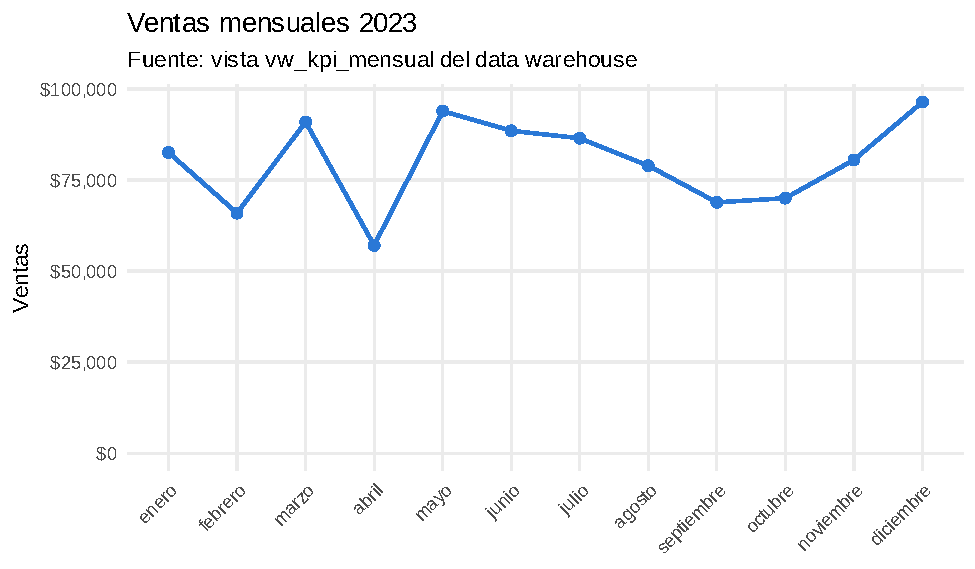
\includegraphics[width=0.9\textwidth]{m05-ventas-mensuales}
\caption{Ventas mensuales calculadas con SQL a partir del data warehouse.}
\label{fig:m05-ventas-mensuales}
\end{figure}

\subsubsection{Pregunta 2. Productos que más venden y su margen}

\begin{rcode}
dbGetQuery(con, "
  SELECT p.nombre_producto, p.categoria,
         SUM(f.cantidad)                            AS unidades,
         ROUND(SUM(f.total), 0)                     AS ventas,
         ROUND(SUM(f.margen), 0)                    AS margen,
         ROUND(100.0 * SUM(f.margen) / SUM(f.total), 1) AS margen_pct
  FROM fact_ventas AS f
  JOIN dim_producto AS p ON f.producto_id = p.producto_id
  GROUP BY p.producto_id
  ORDER BY ventas DESC
  LIMIT 5
")
\end{rcode}

\begin{rsalida}
  nombre_producto  categoria unidades ventas margen margen_pct
1     Producto 06   Juguetes       82  34028  27095       79.6
2     Producto 19   Deportes       85  28368   7557       26.6
3     Producto 31  Alimentos       74  25430  23622       92.9
4     Producto 47 Automotriz       82  24527  20017       81.6
5     Producto 46 Automotriz       74  24470  11333       46.3
\end{rsalida}

El Producto 06 (Juguetes) lidera en ventas y además deja un margen de
79.6\%. En cambio, el Producto 19 (Deportes), segundo en ventas, apenas
deja 26.6\%: vende mucho pero aporta poco. Un producto que vende mucho no
necesariamente es el más rentable.

\begin{rcode}
# ¿Hay productos que se venden con pérdida?
dbGetQuery(con, "
  SELECT p.nombre_producto, p.costo,
         ROUND(AVG(f.precio_venta), 2) AS precio_venta_prom,
         ROUND(SUM(f.margen), 0)       AS margen_total
  FROM fact_ventas AS f
  JOIN dim_producto AS p ON f.producto_id = p.producto_id
  GROUP BY p.producto_id
  HAVING SUM(f.margen) < 0
  ORDER BY margen_total
")
\end{rcode}

\begin{rsalida}
  nombre_producto  costo precio_venta_prom margen_total
1     Producto 13 392.63            257.58        -8602
2     Producto 35 353.50            230.62        -6530
3     Producto 41 389.86            294.97        -6046
4     Producto 12 368.62            296.11        -4332
5     Producto 02 399.12            304.00        -4137
6     Producto 29 391.67            355.31        -2258
7     Producto 10 283.26            260.12        -1282
\end{rsalida}

Siete productos se vendieron con pérdida en el año: su costo unitario es
mayor que el precio promedio al que se vendieron. El Producto 13, por
ejemplo, cuesta \$392.63 y se vendió en promedio a \$257.58, con una
pérdida acumulada de \$8\,602. Es el hallazgo de calidad de datos que ya
conocías (precios de venta generados sin relación con el costo), pero en
una empresa real sería una alerta roja para el área comercial.

\subsubsection{Pregunta 3. Clientes más valiosos}

\begin{rcode}
dbGetQuery(con, "
  SELECT c.nombre, c.ciudad, c.segmento,
         CASE c.es_premium WHEN 1 THEN 'Sí' ELSE 'No' END AS premium,
         COUNT(*)               AS compras,
         ROUND(SUM(f.total), 0) AS gasto,
         ROUND(SUM(f.margen), 0) AS margen
  FROM fact_ventas AS f
  JOIN dim_cliente AS c ON f.cliente_id = c.cliente_id
  GROUP BY c.cliente_id
  ORDER BY gasto DESC
  LIMIT 5
")
\end{rcode}

\begin{rsalida}
          nombre      ciudad segmento premium compras gasto margen
1     Pedro Cruz      Toluca   Adulto      No      13 14680   5882
2  Pedro Morales        León   Senior      No       9 12504   8669
3 Carmen Jiménez Guadalajara   Adulto      No       9 11848   5001
4 Sofia González      Cancún   Maduro      No      12 11676   6778
5  Alberto Reyes Guadalajara   Maduro      No      13 11356   5905
\end{rsalida}

Pedro Cruz, de Toluca, es el cliente más valioso por gasto (\$14\,680 en 13
compras); es el cliente 5 que ya habíamos visto. Pero si ordenamos por
margen, Pedro Morales, de León, deja más (\$8\,669 con solo 9 compras). Un
dato curioso: ninguno de los cinco es cliente premium, una pista para
revisar los criterios del programa.

\subsubsection{Pregunta 4. Productividad de las tiendas}

\begin{rcode}
dbGetQuery(con, "
  SELECT t.nombre_tienda, t.tipo, t.tamano_m2,
         ROUND(SUM(f.total), 0)               AS ventas,
         ROUND(SUM(f.total) / t.tamano_m2, 1) AS ventas_m2,
         ROUND(AVG(f.total), 0)               AS ticket_prom
  FROM fact_ventas AS f
  JOIN dim_tienda AS t ON f.tienda_id = t.tienda_id
  GROUP BY t.tienda_id
  ORDER BY ventas_m2 DESC
")
\end{rcode}

\begin{rsalida}
      nombre_tienda      tipo tamano_m2 ventas ventas_m2 ticket_prom
1  Sucursal Express   Express       300 102791     342.6         952
2   Sucursal Outlet    Outlet       350 114377     326.8        1079
3     Sucursal Este  Estándar       400  88420     221.0         941
4    Sucursal Norte  Estándar       450  89024     197.8         899
5   Sucursal Centro Principal       500  88414     176.8        1016
6      Sucursal Sur  Estándar       600 105305     175.5         966
7  Sucursal Plaza B  Estándar       480  80236     167.2         944
8    Sucursal Oeste  Estándar       550  84672     153.9         891
9  Sucursal Plaza A Principal       700 105216     150.3         965
10 Sucursal Premium   Premium       800 101538     126.9         940
\end{rsalida}

Por metro cuadrado, las tiendas pequeñas ganan: la Sucursal Express
(300~m²) vende \$342.6 por m² y el Outlet \$326.8, mientras que la Sucursal
Premium, la más grande (800~m²), queda al final con \$126.9. Las ventas
totales son parecidas entre tiendas, así que el tamaño no se traduce en más
ventas: una conclusión valiosa para decidir el tamaño de las próximas
aperturas.

\subsubsection{Pregunta 5. Los dos mejores vendedores de cada zona}

Aquí combinamos una CTE con una función de ventana particionada por zona.
Un vendedor puede vender en tiendas de varias zonas, así que el ranking es
``por lo que vendió en esa zona''.

\begin{rcode}
dbGetQuery(con, "
  WITH ventas_vendedor_zona AS (
    SELECT t.zona, v.nombre AS vendedor, SUM(f.total) AS ventas
    FROM fact_ventas AS f
    JOIN dim_tienda   AS t ON f.tienda_id   = t.tienda_id
    JOIN dim_vendedor AS v ON f.vendedor_id = v.vendedor_id
    GROUP BY t.zona, v.vendedor_id
  ),
  ranking AS (
    SELECT zona, vendedor, ROUND(ventas, 0) AS ventas,
           RANK() OVER (PARTITION BY zona ORDER BY ventas DESC) AS lugar
    FROM ventas_vendedor_zona
  )
  SELECT * FROM ranking
  WHERE lugar <= 2
  ORDER BY zona, lugar
")
\end{rcode}

\begin{rsalida}
     zona        vendedor ventas lugar
1  Centro   Isabel García  21198     1
2  Centro    Sofia Rivera  17066     2
3    Este  Fernando Pérez   8881     1
4    Este   Pedro Morales   7589     2
5   Norte Ricardo Ramírez  22238     1
6   Norte  Marta González  21909     2
7   Oeste   Isabel García  11709     1
8   Oeste    Juan Sánchez  10093     2
9     Sur     Marta Gómez  11526     1
10    Sur    Marta Rivera   9124     2
\end{rsalida}

Ricardo Ramírez lidera la zona Norte (\$22\,238) y Isabel García aparece
como la mejor vendedora \emph{en dos zonas} (Centro y Oeste), señal de que
atiende en varias sucursales. En la zona Este, con una sola tienda, las
cifras son mucho menores. Recuerda el hallazgo anterior: varios de estos
``vendedores'' no pertenecen al departamento de Ventas.

\subsubsection{Pregunta 6. Crecimiento mes contra mes}

\begin{rcode}
dbGetQuery(con, "
  SELECT nombre_mes, ventas,
         ROUND(100.0 * (ventas - LAG(ventas) OVER (ORDER BY mes)) /
               LAG(ventas) OVER (ORDER BY mes), 1) AS crec_ventas_pct,
         ROUND(100.0 * (margen - LAG(margen) OVER (ORDER BY mes)) /
               LAG(margen) OVER (ORDER BY mes), 1) AS crec_margen_pct
  FROM vw_kpi_mensual
  ORDER BY mes
")
\end{rcode}

\begin{rsalida}
   nombre_mes   ventas crec_ventas_pct crec_margen_pct
1       enero 82559.66              NA              NA
2     febrero 65899.34           -20.2           -15.1
3       marzo 90930.61            38.0            59.4
4       abril 57037.74           -37.3           -57.4
5        mayo 93910.21            64.6           150.0
6       junio 88509.12            -5.8           -15.1
7       julio 86456.05            -2.3            -2.2
8      agosto 78929.49            -8.7           -19.1
9  septiembre 68855.87           -12.8           -11.4
10    octubre 70004.10             1.7             7.5
11  noviembre 80506.89            15.0            15.4
12  diciembre 96393.61            19.7            39.1
\end{rsalida}

El margen se mueve mucho más que las ventas: en mayo las ventas crecieron
64.6\% pero el margen 150\%, y en abril las ventas cayeron 37.3\% y el
margen 57.4\%. Es decir, la mezcla de productos vendidos cambia de un mes a
otro, y los meses buenos lo son también por vender productos más
rentables.

\subsubsection{Pregunta 7. Fin de semana contra entre semana}

\begin{rcode}
dbGetQuery(con, "
  SELECT CASE d.es_fin_semana WHEN 1 THEN 'Fin de semana'
                              ELSE 'Entre semana' END AS tipo_dia,
         COUNT(DISTINCT d.fecha_id)                    AS dias,
         COUNT(*)                                      AS tickets,
         ROUND(1.0 * COUNT(*) / COUNT(DISTINCT d.fecha_id), 2)
                                                  AS tickets_por_dia,
         ROUND(AVG(f.total), 2)                        AS ticket_prom
  FROM fact_ventas AS f
  JOIN dim_fecha AS d ON f.fecha_id = d.fecha_id
  GROUP BY tipo_dia
")
\end{rcode}

\begin{rsalida}
       tipo_dia dias tickets tickets_por_dia ticket_prom
1  Entre semana  246     724            2.94      961.49
2 Fin de semana   99     276            2.79      956.07
\end{rsalida}

Hubo ventas en 246 días entre semana y 99 de fin de semana (345 días en
total: 20 días del año no registraron ninguna venta). Entre semana se
venden 2.94 tickets por día contra 2.79 en fin de semana, y el ticket
promedio es prácticamente igual (\$961 contra \$956). No hay un patrón de
fin de semana marcado. Este tipo de pregunta es trivial gracias a la dimensión de
fechas: el atributo \codigo{es\_fin\_semana} ya está calculado y cualquier
analista puede usarlo sin saber manipular fechas.

\begin{negocio}{Qué entregarías en la junta}
Con estas siete consultas tienes el material de un reporte ejecutivo
completo, y la base \archivo{bi\_retail.sqlite} queda como la fuente única
de la verdad: el Módulo~\ref{cap:shiny} construirá un tablero que lee de
ella y el Módulo~\ref{cap:reportes} un reporte automático. Lo más valioso
no son las cifras de hoy, sino que el próximo mes basta ejecutar
\codigo{ejecutar\_etl()} con el archivo nuevo y volver a correr las
consultas.
\end{negocio}

\begin{hazlotu}
Agrega una octava pregunta: ¿qué método de pago predomina en cada zona?
Usa \codigo{vw\_ventas\_detalle} y \codigo{ROW\_NUMBER()} particionado por
zona.
\end{hazlotu}

% ----------------------------------------------------------------------------
\section{Errores comunes}
\label{sec:m5-errores}

Para ver los mensajes reales sin detener el script, usamos esta pequeña
función que ejecuta una expresión y, si falla, imprime el mensaje de error
(o de advertencia) en lugar de detenerse:

\begin{rcode}
mostrar_error <- function(expr) {
  tryCatch(expr,
           error   = function(e) cat("Error:", conditionMessage(e), "\n"),
           warning = function(w) cat("Aviso:", conditionMessage(w), "\n"))
}
\end{rcode}

\subsubsection{``no such table'' y ``no such column''}

\begin{rcode}
mostrar_error(dbGetQuery(con, "SELECT * FROM ventas_2024"))
mostrar_error(dbGetQuery(con, "SELECT totl FROM fact_ventas"))
\end{rcode}

\begin{rsalida}
Error: no such table: ventas_2024 
Error: no such column: totl 
\end{rsalida}

La tabla o la columna no existe, casi siempre por un error de dedo o
porque estás conectado a otra base. Revisa con \codigo{dbListTables(con)} y
\codigo{dbListFields(con, "tabla")}. Recuerda también que, tras reconstruir
la base, las tablas crudas (\codigo{transacciones}, \codigo{clientes}\ldots)
ya no existen: solo el esquema en estrella.

\subsubsection{La tabla ya existe}

\begin{rcode}
mostrar_error(dbWriteTable(con, "dim_tienda", dimensiones$dim_tienda))
\end{rcode}

\begin{rsalida}
Error: Table dim_tienda exists in database, and both overwrite and append are FALSE 
\end{rsalida}

\codigo{dbWriteTable()} se niega a pisar una tabla existente. Decide qué
quieres: \codigo{overwrite = TRUE} la reemplaza (¡perdiendo llaves y
reglas si la habías creado con \codigo{CREATE TABLE}!) y
\codigo{append = TRUE} agrega filas. Para tablas diseñadas por ti, usa
\codigo{dbAppendTable()}.

\subsubsection{Llaves duplicadas al volver a cargar}

\begin{rcode}
mostrar_error(dbAppendTable(con, "dim_tienda", dimensiones$dim_tienda))
\end{rcode}

\begin{rsalida}
Error: UNIQUE constraint failed: dim_tienda.tienda_id 
\end{rsalida}

Intentaste cargar filas cuya llave primaria ya existe (típico al correr dos
veces un script). Usa carga incremental (\codigo{anti\_join()} o
\codigo{INSERT OR IGNORE}) o borra primero lo que vas a recargar.

\subsubsection{Fechas convertidas en números}

Si ves fechas como \codigo{19370} o años como \codigo{-4672}, escribiste un
\codigo{Date} de R directamente en SQLite (sección~\ref{sec:m5-fechas}).
Convierte las fechas a texto con \codigo{format(fecha, "\%Y-\%m-\%d")}
antes de escribirlas y con \codigo{as.Date()} al leerlas.

\subsubsection{Comillas simples contra comillas dobles}

En SQL estándar, el texto va entre comillas \emph{simples}
(\codigo{'CDMX'}) y las comillas \emph{dobles} son para nombres de
columnas o tablas. SQLite, por compatibilidad, acepta comillas dobles para
texto si no encuentra una columna con ese nombre, lo que produce errores
silenciosos:

\begin{rcode}
dbGetQuery(con, "SELECT COUNT(*) AS n FROM dim_cliente
                 WHERE ciudad = 'CDMX'")     # correcto: 27
dbGetQuery(con, "SELECT COUNT(*) AS n FROM dim_cliente
                 WHERE ciudad = \"ciudad\"")  # ¡columna consigo misma!
\end{rcode}

\begin{rsalida}
   n
1 27
    n
1 200
\end{rsalida}

La segunda consulta pretendía buscar clientes de una ciudad llamada
``ciudad'', pero \codigo{"ciudad"} se interpretó como la \emph{columna}
ciudad, que siempre es igual a sí misma: devolvió los 200 clientes. En
PostgreSQL o SQL Server, \codigo{"CDMX"} directamente marcaría error de
columna inexistente. Usa siempre comillas simples para texto (y
\codigo{params} para valores variables).

\subsubsection{Olvidar cerrar conexiones y resultados}

\begin{rcode}
con_temporal <- dbConnect(RSQLite::SQLite(), ":memory:")
dbDisconnect(con_temporal)
mostrar_error(dbGetQuery(con_temporal, "SELECT 1"))
\end{rcode}

\begin{rsalida}
Error: Invalid or closed connection 
\end{rsalida}

Usar una conexión ya cerrada da \codigo{Invalid or closed connection}: vuelve
a conectarte. El error contrario (nunca cerrar) no da error inmediato, pero
R te avisa más tarde con un mensaje como \emph{call dbDisconnect() when
finished working with a connection}, y en un servidor acumula conexiones
abiertas. Usa \codigo{dbDisconnect()} al final de cada script y
\codigo{on.exit()} dentro de las funciones. Del mismo modo, cada
\codigo{dbSendQuery()} necesita su \codigo{dbClearResult()}.

\begin{table}[H]
\centering
\small
\caption{Resumen de errores frecuentes con bases de datos.}
\label{tab:m5-errores}
\begin{tabularx}{\textwidth}{@{}>{\raggedright\arraybackslash}p{5.2cm}X@{}}
\toprule
\textbf{Mensaje o síntoma} & \textbf{Causa y solución} \\
\midrule
\codigo{no such table: X} & La tabla no existe o estás en otra base.
Revisa \codigo{dbListTables()}. \\
\codigo{no such column: X} & Error de dedo o columna de otra tabla; revisa
\codigo{dbListFields()} y los alias. \\
\codigo{ambiguous column name: X} & La columna existe en dos tablas del
JOIN: antepón el alias (\codigo{t.producto\_id}). \\
\codigo{Table X exists in database\ldots} & Usa \codigo{overwrite},
\codigo{append} o \codigo{dbAppendTable()}. \\
\codigo{UNIQUE constraint failed} & Llave repetida: carga incremental o
\codigo{INSERT OR IGNORE}. \\
\codigo{FOREIGN KEY constraint failed} & Un valor no existe en la
dimensión: carga primero las dimensiones o corrige el dato. \\
Fechas como números & Convierte \codigo{Date} a texto ISO antes de
escribir. \\
\codigo{Invalid or closed connection} & La conexión se cerró: vuelve a
conectarte. \\
Resultados ``demasiado buenos'' & Comillas dobles en lugar de simples, o
un JOIN que multiplica filas. \\
\bottomrule
\end{tabularx}
\end{table}

Terminamos cerrando la conexión principal del módulo:

\begin{rcode}
dbDisconnect(con)
\end{rcode}

% ----------------------------------------------------------------------------
\begin{resumen}
\begin{itemize}
  \item Las empresas guardan sus datos en bases de datos por volumen,
        integridad, concurrencia y seguridad. Las OLTP operan el negocio;
        los \emph{data warehouses} (OLAP) sirven para analizarlo.
  \item \paquete{DBI} ofrece las mismas funciones para cualquier motor:
        \codigo{dbConnect()}, \codigo{dbWriteTable()},
        \codigo{dbGetQuery()}, \codigo{dbExecute()},
        \codigo{dbDisconnect()}. Solo cambia el driver.
  \item En SQLite guarda las fechas como texto \codigo{'AAAA-MM-DD'}; si no,
        se vuelven números.
  \item SQL: \codigo{SELECT}, \codigo{WHERE}, \codigo{GROUP BY},
        \codigo{HAVING}, \codigo{ORDER BY}, \codigo{JOIN}, subconsultas,
        CTE y funciones de ventana responden casi cualquier pregunta.
  \item Nunca pegues valores del usuario con \codigo{paste()}: usa
        \codigo{params}, \codigo{glue\_sql()} o \codigo{sqlInterpolate()}.
  \item \paquete{dbplyr} traduce dplyr a SQL; \codigo{show\_query()} te
        enseña el SQL y \codigo{collect()} trae el resultado.
  \item Un data warehouse en estrella tiene una tabla de hechos y
        dimensiones con llaves declaradas, vistas para los KPIs e índices
        en las llaves.
  \item Un ETL confiable es idempotente (sin duplicados), atómico
        (transacciones) y trazable (bitácora).
  \item Con datos grandes: agrega en la base, trae solo lo necesario y usa
        \codigo{dbFetch()} por bloques.
  \item Credenciales en \archivo{.Renviron}, nunca en el script; usuarios de
        solo lectura para analizar.
\end{itemize}

\medskip
\centering
\small
\begin{tabular}{@{}ll@{}}
\toprule
\textbf{SQL} & \textbf{dplyr} \\
\midrule
\codigo{SELECT col1, col2} & \codigo{select(col1, col2)} \\
\codigo{SELECT expr AS nueva} & \codigo{mutate(nueva = expr)} \\
\codigo{WHERE cond} & \codigo{filter(cond)} \\
\codigo{ORDER BY col DESC} & \codigo{arrange(desc(col))} \\
\codigo{LIMIT 5} & \codigo{head(5)} / \codigo{slice\_head(n = 5)} \\
\codigo{GROUP BY g} + \codigo{SUM(x)} & \codigo{group\_by(g)} +
  \codigo{summarise(sum(x))} \\
\codigo{HAVING cond} & \codigo{filter()} después de \codigo{summarise()} \\
\codigo{COUNT(DISTINCT x)} & \codigo{n\_distinct(x)} \\
\codigo{CASE WHEN \ldots{} END} & \codigo{case\_when()} \\
\codigo{INNER JOIN} / \codigo{LEFT JOIN} & \codigo{inner\_join()} /
  \codigo{left\_join()} \\
\codigo{LEFT JOIN \ldots{} WHERE b.id IS NULL} & \codigo{anti\_join()} \\
\codigo{WITH paso AS (\ldots)} & guardar un resultado intermedio \\
\codigo{ROW\_NUMBER() OVER (PARTITION BY g \ldots)} & \codigo{group\_by(g)}
  + \codigo{row\_number()} \\
\codigo{SUM(x) OVER (ORDER BY t)} & \codigo{cumsum(x)} \\
\codigo{LAG(x) OVER (ORDER BY t)} & \codigo{lag(x)} \\
\bottomrule
\end{tabular}
\end{resumen}

% ----------------------------------------------------------------------------
\section{Ejercicios}
\label{sec:m5-ejercicios}

Resuelve cada ejercicio en un script nuevo. Para no depender de la base del
capítulo, trabaja con una base en memoria
(\codigo{dbConnect(RSQLite::SQLite(), ":memory:")}) y carga solo las tablas
que necesites. Salvo que se indique otra cosa, responde con SQL escrito a
mano mediante \codigo{dbGetQuery()}.

\begin{ejercicio}{m5-1}{Tu primera base de datos}
\nivel{Básico}
Crea una base en memoria, carga \archivo{productos.csv} en una tabla
llamada \codigo{productos} y muestra sus tablas y columnas con
\codigo{dbListTables()} y \codigo{dbListFields()}. Después, con SQL,
calcula cuántos productos hay por categoría y el precio de catálogo
promedio, ordenado de más a menos productos. Cierra la conexión al final.
\end{ejercicio}

\begin{ejercicio}{m5-2}{Alerta de inventario}
\nivel{Básico}
El área de compras necesita la lista de productos \emph{activos} cuyo
\codigo{stock\_actual} está por debajo del \codigo{stock\_minimo}. Muestra
nombre, categoría, proveedor, stock actual, stock mínimo y las piezas
faltantes (\codigo{stock\_minimo - stock\_actual}), ordenado de mayor a
menor faltante. ¿Cuántos productos están en alerta y qué proveedor
aparece más?
\end{ejercicio}

\begin{ejercicio}{m5-3}{Nómina por departamento}
\nivel{Básico}
Con \archivo{empleados.csv}, calcula por departamento: número de
empleados, salario mensual promedio y salario máximo. Muestra solo los
departamentos con al menos 15 empleados (\codigo{HAVING}), ordenados por
salario promedio descendente.
\end{ejercicio}

\begin{ejercicio}{m5-4}{Ventas por ciudad y productos sin ventas en diciembre}
\nivel{Intermedio}
Carga \archivo{transacciones.csv}, \archivo{tiendas.csv} y
\archivo{productos.csv} (con fechas como texto ISO). (a) Con un
\codigo{INNER JOIN}, calcula por ciudad de la tienda el número de tickets,
las ventas y el ticket promedio. (b) Con un \codigo{LEFT JOIN}, encuentra
los productos que no tuvieron ninguna venta en diciembre de 2023.
\end{ejercicio}

\begin{ejercicio}{m5-5}{Fechas bien guardadas}
\nivel{Intermedio}
Carga \archivo{ventas\_retail.csv} dos veces en una base en memoria: una
tabla \codigo{ventas\_mal} con la fecha tal como la lee
\codigo{read\_csv()} y otra \codigo{ventas} con la fecha como texto ISO.
Demuestra con \codigo{typeof()} y \codigo{strftime()} la diferencia. Luego,
con la tabla correcta, calcula por trimestre (a partir de la fecha) las
ventas totales, el descuento promedio y el número de días con descuento.
\end{ejercicio}

\begin{ejercicio}{m5-6}{Consulta segura de un cliente}
\nivel{Intermedio}
Escribe una función \codigo{ventas\_cliente(con, cliente, desde, hasta)}
que devuelva el número de compras y el gasto de un cliente en un periodo,
usando una consulta parametrizada con marcadores con nombre. Pruébala con
el cliente 5 en el primer semestre de 2023 y en el segundo. Después
demuestra que el texto \codigo{"5 OR 1=1"} no logra traer las compras de
todos los clientes.
\end{ejercicio}

\begin{ejercicio}{m5-7}{Lo mismo con dbplyr}
\nivel{Intermedio}
Con \paquete{dbplyr}, calcula para cada método de pago y trimestre el
número de tickets y las ventas, a partir de la tabla \codigo{transacciones}.
Muestra el SQL generado con \codigo{show\_query()}, trae el resultado con
\codigo{collect()} y comprueba con \codigo{all.equal()} que coincide con
la misma consulta escrita a mano en SQL.
\end{ejercicio}

\begin{ejercicio}{m5-8}{Rankings y Pareto con funciones de ventana}
\nivel{Avanzado}
(a) Encuentra los dos clientes con mayor gasto de cada ciudad (ciudad del
cliente) usando \codigo{RANK()} con \codigo{PARTITION BY}; muestra solo
Monterrey, Guadalajara y CDMX. (b) Construye la curva de Pareto de
productos: ordena los productos por ventas y calcula con
\codigo{SUM() OVER} el porcentaje acumulado. ¿Cuántos productos generan el
80\% de las ventas?
\end{ejercicio}

\begin{ejercicio}{m5-9}{Una estrella en miniatura}
\nivel{Avanzado}
A partir de \archivo{ventas\_retail.csv}, \archivo{productos.csv} y
\archivo{tiendas.csv}, crea en una base en memoria un esquema en estrella
pequeño: \codigo{dim\_producto}, \codigo{dim\_tienda} y
\codigo{fact\_ventas\_diarias} (llave primaria \codigo{fecha}, llaves
foráneas a ambas dimensiones, \codigo{CHECK (cantidad > 0)}). Carga los
datos con \codigo{dbAppendTable()}, crea una vista con las ventas por
trimestre y tipo de tienda, y muestra con \codigo{EXPLAIN QUERY PLAN} el
efecto de un índice sobre \codigo{tienda\_id}.
\end{ejercicio}

\begin{ejercicio}{m5-10}{ETL incremental con bitácora}
\nivel{Reto}
Construye un ETL para \archivo{ventas\_retail.csv} en una base en memoria:
una tabla \codigo{fact\_ventas\_diarias} con llave primaria \codigo{fecha}
(texto) y una tabla \codigo{log\_etl}. Escribe las funciones
\codigo{extraer\_ventas()}, \codigo{transformar\_ventas()},
\codigo{cargar\_ventas()} (que inserte desde una tabla temporal solo las
fechas que aún no existen) y \codigo{ejecutar\_etl()} (con transacción y registro en la
bitácora, también de los errores). Simula tres lotes: enero-junio,
abril-septiembre (traslapado) y octubre-diciembre; ejecuta además un lote
repetido y un lote con una cantidad negativa que debe ser rechazado por la
regla \codigo{CHECK}. Muestra la bitácora y verifica que la tabla termina
con exactamente 365 filas y el mismo total de ventas que el CSV.
\end{ejercicio}

% ============================================================================
% MÓDULO 6. DASHBOARDS INTERACTIVOS CON SHINY
% ============================================================================
\chapter{Dashboards interactivos con Shiny}
\label{cap:shiny}

\begin{objetivos}
\begin{itemize}
  \item Explicar qué hace bueno a un dashboard de BI (audiencia, preguntas,
        KPIs, filtros) y decidir cuándo conviene Shiny y cuándo Power BI o
        Tableau.
  \item Entender la anatomía de una app Shiny (\codigo{ui}, \codigo{server},
        \codigo{shinyApp()}) y ejecutar las tres apps completas que acompañan
        este módulo.
  \item Usar las entradas y salidas más comunes y saber qué función
        \codigo{render...()} corresponde a cada \codigo{...Output()}.
  \item Dominar la \termino{reactividad}: \codigo{reactive()},
        \codigo{observeEvent()}, \codigo{eventReactive()}, \codigo{req()},
        \codigo{validate()} e \codigo{isolate()}, y reconocer sus errores
        típicos.
  \item Organizar la pantalla con \codigo{sidebarLayout()},
        \codigo{fluidRow()}, pestañas y \paquete{shinydashboard}
        (\codigo{valueBox()}, \codigo{box()}, menús).
  \item Agregar tablas interactivas con \paquete{DT}, botones de descarga en
        CSV y Excel, y gráficas interactivas con \paquete{plotly}.
  \item Aplicar buenas prácticas profesionales: separar la lógica de la
        interfaz, módulos, caché, pruebas con \codigo{testServer()} y
        publicación segura.
\end{itemize}
\end{objetivos}

Llevas cinco módulos respondiendo preguntas de negocio con R. Cada vez que la
directora comercial te pide algo (``¿cuánto vendimos en Monterrey en el
segundo trimestre?'', ``¿y solo en Electrónica?'', ``¿y si quitamos el
Outlet?'') tú abres RStudio, cambias un \codigo{filter()}, vuelves a correr
el script y le mandas una gráfica nueva por correo. Funciona, pero no escala:
tú te conviertes en el cuello de botella y ella espera horas por una
respuesta que le tomaría segundos si pudiera mover los filtros por sí misma.

La solución es un \termino{dashboard interactivo}: una página web donde la
directora elige el periodo, la tienda y la categoría, y las cifras y
gráficas se actualizan al instante. Con el paquete \paquete{shiny} puedes
construirlo \emph{con el mismo R que ya sabes}: tus \codigo{filter()},
\codigo{summarise()} y \codigo{ggplot()} siguen siendo el corazón; Shiny solo
añade la ``piel'' (botones, menús, cajas) y el ``sistema nervioso'' (la
reactividad) que conecta lo que el usuario toca con lo que R calcula.

En este módulo construirás tres apps de complejidad creciente, que vienen
completas en la carpeta \archivo{latex/codigo/apps/} del curso: una
calculadora de precios (tu primera app), un explorador de ventas con filtros
y un dashboard ejecutivo con cinco pestañas, indicadores, tablas y botones de
descarga. Al final tendrás la base del dashboard del proyecto integrador
(Módulo~\ref{cap:proyecto}).

% ----------------------------------------------------------------------------
\section{¿Qué es un dashboard de BI y qué lo hace bueno?}
\label{sec:m6-dashboard}

\begin{concepto}{Dashboard de BI}
Un \termino{dashboard} (tablero de control) es una pantalla que reúne los
indicadores más importantes de un negocio para que una audiencia concreta
pueda \emph{monitorear} cómo va y \emph{decidir} qué hacer, de un vistazo.
Un \termino{KPI} (\emph{Key Performance Indicator}, indicador clave de
desempeño) es una cifra que resume algo que importa: ventas, ticket
promedio, clientes activos, margen. Un dashboard \emph{interactivo} además
deja filtrar y profundizar sin pedirle nada al analista.
\end{concepto}

Un dashboard no es ``poner todas las gráficas que tengo en una pantalla''.
Los buenos comparten cinco rasgos:

\begin{enumerate}
  \item \textbf{Tiene una audiencia definida.} El director general quiere
        cinco cifras y una tendencia; el gerente de tienda quiere detalle de
        su sucursal; el analista quiere descargar datos. Un dashboard para
        ``todos'' no le sirve bien a nadie.
  \item \textbf{Responde preguntas concretas.} Antes de programar, escribe
        las 3--5 preguntas que debe contestar (``¿vamos arriba o abajo del
        mes pasado?'', ``¿qué tienda jala hacia abajo?''). Cada elemento de
        la pantalla debe responder a una de ellas.
  \item \textbf{Pone los KPIs arriba.} La vista sigue un patrón en ``Z'': lo
        primero que se lee es la esquina superior izquierda. Ahí van las
        cifras principales en tarjetas grandes; debajo, las tendencias; al
        final, el detalle (tablas).
  \item \textbf{Agrupa los filtros en un solo lugar.} Todos los filtros
        juntos (en una barra lateral o en una fila arriba), con valores por
        defecto sensatos (``todo el año'', ``todas las tiendas'') y que
        afecten a toda la página por igual.
  \item \textbf{Menos es más.} Pocas gráficas, bien elegidas, con un solo
        color salvo que el color signifique algo, ejes con formato de negocio
        (\$, \%, miles) y títulos que digan qué mirar. Lo que aprendiste en el
        Módulo~\ref{cap:visualizacion} aplica aquí multiplicado.
\end{enumerate}

La figura~\ref{fig:m6-anatomia-dashboard} resume esa jerarquía visual. La
usaremos como plantilla para el dashboard ejecutivo de la
sección~\ref{sec:m6-shinydashboard}.

\begin{figure}[H]
\centering
\begin{tikzpicture}[
    font=\sffamily\small,
    zona/.style={draw=gristexto!60, rounded corners=2pt, align=center},
    kpi/.style={zona, fill=primario!12, minimum width=2.55cm, minimum height=1.1cm},
    graf/.style={zona, fill=secundario!10},
    nota/.style={font=\sffamily\footnotesize, text=gristexto, align=left, anchor=west}]
  % marco de la pantalla
  \draw[gristexto, rounded corners=3pt, line width=0.8pt] (0,0) rectangle (11.2,7);
  \fill[primario!85] (0,6.4) rectangle (11.2,7);
  \node[white, anchor=west] at (0.2,6.7) {\textbf{Ventas 2023}};
  % filtros
  \node[zona, fill=acento!12, minimum width=10.8cm, minimum height=0.6cm,
        anchor=north west] at (0.2,6.2)
        {Filtros: \ periodo \quad tienda \quad categoría \quad [Quitar filtros]};
  % kpis
  \foreach \i/\t/\v in {0/Ventas/\$959,993, 1/Transacciones/1{,}000,
                        2/Ticket promedio/\$960, 3/Clientes/198} {
    \node[kpi, anchor=north west] at ({0.2+\i*2.72},5.35)
      {\textbf{\v}\\[-1pt]{\footnotesize \t}};
  }
  % graficas
  \node[graf, minimum width=6.9cm, minimum height=2.2cm, anchor=north west]
       at (0.2,4.0) {Tendencia mensual\\(línea)};
  \node[graf, minimum width=3.7cm, minimum height=2.2cm, anchor=north west]
       at (7.3,4.0) {Composición\\(barras)};
  % tabla
  \node[zona, fill=gray!8, minimum width=10.8cm, minimum height=1.35cm,
        anchor=north west] at (0.2,1.6) {Detalle: tabla con búsqueda y descarga};
  % numeración de lectura
  \foreach \y/\n in {5.9/1, 4.8/2, 2.9/3, 0.9/4} {
    \node[circle, fill=acento, text=white, inner sep=1.5pt, font=\sffamily\scriptsize\bfseries]
      at (11.55,\y) {\n};
  }
  \node[nota] at (11.8,5.9) {Filtros en un\\solo lugar};
  \node[nota] at (11.8,4.8) {KPIs arriba};
  \node[nota] at (11.8,2.9) {Tendencias y\\comparaciones};
  \node[nota] at (11.8,0.9) {Detalle al final};
\end{tikzpicture}
\caption{Jerarquía de un buen dashboard: filtros juntos, KPIs arriba,
tendencias en medio y detalle al final.}
\label{fig:m6-anatomia-dashboard}
\end{figure}

\begin{negocio}{Tres dashboards, tres audiencias}
En una cadena de retail es común tener al menos tres vistas de los mismos
datos: (1) un \emph{dashboard ejecutivo} para la dirección, con 4--6 KPIs,
la tendencia contra el año anterior y el ranking de tiendas; (2) un
\emph{dashboard operativo} para gerentes de tienda, filtrado a su sucursal,
con ventas del día, inventario bajo y desempeño por vendedor; y (3) un
\emph{explorador analítico} para el equipo de BI, con muchos filtros, tablas
detalladas y descarga de datos. Mismo origen, distinto diseño.
\end{negocio}

\subsection{Shiny frente a Power BI y Tableau}

Seguramente conoces herramientas como Power BI o Tableau, que permiten armar
dashboards arrastrando campos con el ratón. ¿Por qué aprender Shiny? No se
trata de que una herramienta sea mejor que otra, sino de elegir la adecuada
para cada caso (tabla~\ref{tab:m6-shiny-vs-bi}).

\begin{table}[H]
\centering
\caption{Cuándo conviene cada herramienta.}
\label{tab:m6-shiny-vs-bi}
\small
\begin{tabularx}{\textwidth}{>{\raggedright\arraybackslash}p{3.1cm}
                             >{\raggedright\arraybackslash}X
                             >{\raggedright\arraybackslash}X}
\toprule
\textbf{Aspecto} & \textbf{Power BI / Tableau} & \textbf{Shiny (R)} \\
\midrule
Curva de aprendizaje & Baja: arrastrar y soltar & Media: hay que programar \\
Tiempo al primer tablero & Minutos & Una o dos horas \\
Lógica compleja (modelos, simulaciones, pronósticos) & Limitada o con
extensiones & Todo lo que R sabe hacer: \paquete{forecast}, modelos de
Machine Learning, optimización \\
Reproducibilidad y control de versiones & Archivos binarios difíciles de
comparar & Código de texto: Git, revisiones, pruebas automáticas \\
Diseño a la medida & Dentro de lo que ofrece la herramienta & Total (HTML,
CSS, JavaScript si hace falta) \\
Costo & Licencia por usuario & Paquete gratuito; el servidor puede ser
gratuito o de pago \\
Ideal para & Reportes corporativos estándar, autoservicio de usuarios de
negocio & Apps analíticas a la medida, prototipos rápidos para quien ya
trabaja en R, herramientas con modelos \\
\bottomrule
\end{tabularx}
\end{table}

\begin{consejo}
Muchas empresas usan ambos: Power BI o Tableau para los reportes estándar que
consume toda la organización, y Shiny para las herramientas analíticas que
necesitan un modelo o una lógica que esas plataformas no cubren (un
simulador de precios, un pronóstico de demanda, un segmentador de clientes).
Saber Shiny te permite construir justo lo que las otras herramientas no
pueden.
\end{consejo}

% ----------------------------------------------------------------------------
\section{Anatomía de una app Shiny}
\label{sec:m6-anatomia}

\subsection{Instalación}

Los paquetes de este módulo se instalan una sola vez:

\begin{rnoejecutar}
install.packages(c("shiny", "shinydashboard", "DT", "plotly", "writexl"))
\end{rnoejecutar}

A lo largo del módulo usaremos estos paquetes. Cárgalos al inicio de tu
script (al cargar \paquete{shinydashboard} y \paquete{DT} verás avisos de que
``enmascaran'' funciones como \codigo{box()} o \codigo{renderDataTable()}; son
normales):

\begin{rcode}
library(shiny)            # apps web con R
library(shinydashboard)   # plantillas de dashboard
library(DT)               # tablas interactivas
library(tidyverse)        # dplyr, ggplot2, readr...
library(lubridate)        # fechas
library(scales)           # formatos de moneda y porcentaje
options(width = 70)
\end{rcode}

\subsection{Las tres piezas: \texorpdfstring{\codigo{ui}, \codigo{server} y \codigo{shinyApp()}}{ui, server y shinyApp()}}

\begin{concepto}{Estructura de toda app Shiny}
Toda app Shiny tiene tres piezas:
\begin{itemize}
  \item \codigo{ui} (\emph{user interface}): describe lo que el usuario
        \textbf{ve}. Es un objeto de R que en realidad es HTML: títulos,
        cajas de entrada, huecos donde irán las gráficas.
  \item \codigo{server}: una función con los argumentos \codigo{input},
        \codigo{output} y \codigo{session} que contiene la \textbf{lógica}:
        lee lo que el usuario eligió (\codigo{input\$...}) y produce
        resultados (\codigo{output\$...}).
  \item \codigo{shinyApp(ui, server)}: une ambas piezas y crea la app.
\end{itemize}
\end{concepto}

Cuando lanzas una app, R arranca un pequeño \termino{servidor web} en tu
computadora. El navegador pide la página, recibe el HTML de la \codigo{ui} y
abre una conexión permanente (un \termino{WebSocket}) con R. Cada vez que
mueves un control, el navegador envía el nuevo valor; R recalcula
\emph{solo} lo que depende de ese valor y devuelve el resultado
(figura~\ref{fig:m6-flujo}).

\begin{figure}[H]
\centering
\begin{tikzpicture}[
    font=\sffamily\small, >={Stealth[length=2.5mm]},
    caja/.style={draw, rounded corners=3pt, line width=0.8pt, align=center,
                 minimum width=4.6cm, minimum height=3.7cm},
    mini/.style={draw=gristexto!70, rounded corners=1.5pt, fill=white,
                 font=\sffamily\footnotesize, minimum width=3.6cm, align=center}]
  \node[caja, draw=secundario, fill=secundario!6] (nav) at (0,0) {};
  \node[font=\sffamily\bfseries, text=secundario, anchor=north]
       at (nav.north) {Navegador (lo que ve el usuario)};
  \node[mini] (in1) at (0,0.55) {Precio: [ 1200 ]};
  \node[mini] (in2) at (0,-0.15) {Descuento: \textbf{-----o-----} 25\%};
  \node[mini, fill=exito!8] (out1) at (0,-1.05) {Precio final: \$900};
  \node[caja, draw=primario, fill=primario!5] (r) at (8.2,0) {};
  \node[font=\sffamily\bfseries, text=primario, anchor=north]
       at (r.north) {Sesión de R (server)};
  \node[mini, font=\ttfamily\footnotesize] (inr) at (8.2,0.4)
       {input\$precio\\input\$descuento};
  \node[mini, font=\ttfamily\footnotesize, fill=primario!8] (calc) at (8.2,-1.05)
       {output\$precio\_final <-\\renderText(\{...\})};
  \draw[->, thick, acento] (in1.east) to[out=10, in=170]
       node[above, font=\sffamily\scriptsize, text=acento] {1. el usuario cambia un valor} (inr.west);
  \draw[->, thick, primario] (inr.south) -- node[right, font=\sffamily\scriptsize] {2. R recalcula} (calc.north);
  \draw[->, thick, exito] (calc.west) --
       node[below, font=\sffamily\scriptsize, text=exito, align=center] {3. envía el resultado\\(texto, imagen, HTML)} (out1.east);
  \node[font=\sffamily\scriptsize, text=gristexto] at (4.1,-2.35)
       {Conexión permanente (WebSocket) mientras la pestaña esté abierta};
\end{tikzpicture}
\caption{Flujo de una app Shiny: el navegador envía entradas, R recalcula y
devuelve salidas.}
\label{fig:m6-flujo}
\end{figure}

\subsection{Tu primera app paso a paso}
\label{sec:m6-primera-app}

\begin{ejemplo}{Calculadora de precio con descuento}
El área comercial quiere que los vendedores calculen el precio final de un
producto con descuento sin abrir Excel. La app debe tener dos entradas
(precio de lista y porcentaje de descuento) y mostrar el precio final. Está
en \archivo{latex/codigo/apps/01-primera-app/app.R}.
\end{ejemplo}

Este es el archivo completo. Léelo con calma: son apenas 30 líneas de código
útil y contienen todo lo esencial de Shiny.

\begin{rnoejecutar}[title=latex/codigo/apps/01-primera-app/app.R]
# 1. Paquete -------------------------------------------------------------
library(shiny)          # el motor de las apps web con R

# 2. Interfaz (ui): lo que el usuario VE en el navegador -----------------
ui <- fluidPage(                       # página que se adapta al ancho
  titlePanel("Calculadora de precio con descuento"),   # título

  # Entrada 1: una caja para escribir un número (el precio de lista)
  numericInput(inputId = "precio", label = "Precio de lista ($):",
               value = 500, min = 0, step = 10),

  # Entrada 2: un deslizador para elegir el descuento
  sliderInput(inputId = "descuento", label = "Descuento (%):",
              min = 0, max = 50, value = 10, step = 5),

  # Salida: un hueco donde el servidor escribirá el resultado
  h3(textOutput(outputId = "precio_final"))
)

# 3. Servidor (server): la lógica que CORRE en R -------------------------
server <- function(input, output, session) {
  # renderText() se vuelve a ejecutar SOLO cuando cambian las entradas
  # que usa (input$precio o input$descuento): eso es la reactividad
  output$precio_final <- renderText({
    final <- input$precio * (1 - input$descuento / 100)
    paste0("Precio final: ", scales::dollar(final))
  })
}

# 4. Unir interfaz y servidor: esto crea (y lanza) la app ----------------
shinyApp(ui = ui, server = server)
\end{rnoejecutar}

Vamos por partes:

\begin{itemize}
  \item \textbf{Línea 2:} \codigo{library(shiny)} carga el paquete. Toda app
        empieza así.
  \item \textbf{Líneas 5--18, la \codigo{ui}:} \codigo{fluidPage()} crea una
        página que se adapta al ancho de la pantalla (de computadora o de
        celular). Dentro van, separados \emph{por comas}, sus elementos: un
        título, dos \termino{entradas} (\emph{inputs}) y una
        \termino{salida} (\emph{output}).
  \item \textbf{El \codigo{inputId}:} cada entrada tiene un identificador
        único (\codigo{"precio"}, \codigo{"descuento"}). Es el nombre con el
        que el servidor lee su valor: \codigo{input\$precio}.
  \item \textbf{\codigo{textOutput("precio\_final")}:} reserva un hueco en
        la página. No calcula nada; solo dice ``aquí irá un texto llamado
        \codigo{precio\_final}''. Lo envolvemos en \codigo{h3()} para que se
        vea grande (\codigo{h3} es un encabezado de HTML).
  \item \textbf{Líneas 21--28, el \codigo{server}:} es una función. Dentro
        asignamos \codigo{output\$precio\_final} con \codigo{renderText()}.
        El código entre llaves lee \codigo{input\$precio} e
        \codigo{input\$descuento}, calcula y devuelve un texto.
  \item \textbf{La magia:} no escribimos ningún ``cuando el usuario mueva el
        deslizador, recalcula''. Shiny detecta solo que
        \codigo{renderText()} usó esas dos entradas y lo vuelve a ejecutar
        cada vez que alguna cambia. Eso es la \termino{reactividad}.
  \item \textbf{Línea 31:} \codigo{shinyApp()} une las piezas. Si ejecutas
        el archivo, la app se abre.
\end{itemize}

La \codigo{ui} es solo un objeto de R que genera HTML. Puedes construir una
entrada en la consola e imprimirla para ver lo que el navegador recibirá.
Es un gran recurso para entender (y depurar) Shiny:

\begin{rcode}
# Una entrada numérica, igual a la de la app, impresa en la consola
numericInput(inputId = "precio", label = "Precio de lista ($):",
             value = 500, min = 0, step = 10)
\end{rcode}
\begin{rsalida}
<div class="form-group shiny-input-container">
  <label class="control-label" id="precio-label" for="precio">Precio de lista ($):</label>
  <input id="precio" type="number" class="shiny-input-number form-control" value="500" min="0" step="10"/>
</div>
\end{rsalida}

Observa el \codigo{id="precio"}: el \codigo{inputId} se convierte en el
identificador del elemento HTML, y por eso \textbf{debe ser único} en toda la
app. Las salidas son todavía más simples, un contenedor vacío con una clase
especial que Shiny sabe llenar:

\begin{rcode}
textOutput(outputId = "precio_final")
plotOutput(outputId = "grafica", height = "300px")
\end{rcode}
\begin{rsalida}
<div id="precio_final" class="shiny-text-output"></div>
<div class="shiny-plot-output html-fill-item" id="grafica" style="width:100%;height:300px;"></div>
\end{rsalida}

\begin{figure}[H]
\centering
\begin{tikzpicture}[font=\sffamily\small]
  \draw[gristexto, rounded corners=3pt, line width=0.8pt] (0,0) rectangle (9,4.6);
  \fill[gray!12] (0,4.1) rectangle (9,4.6);
  \foreach \x in {0.25,0.5,0.75} \fill[gray!45] (\x,4.35) circle (0.07);
  \node[anchor=west, font=\sffamily\footnotesize, text=gristexto] at (1,4.35) {http://127.0.0.1:XXXX};
  \node[anchor=west, font=\sffamily\Large] at (0.3,3.55) {Calculadora de precio con descuento};
  \node[anchor=west] at (0.3,2.85) {Precio de lista (\$):};
  \draw[gristexto!80, fill=white] (0.3,2.1) rectangle (4.3,2.6);
  \node[anchor=west] at (0.4,2.35) {500};
  \node[anchor=west] at (0.3,1.7) {Descuento (\%):};
  \draw[line width=2pt, secundario!50] (0.4,1.2) -- (4.2,1.2);
  \draw[line width=2pt, secundario] (0.4,1.2) -- (1.16,1.2);
  \fill[white, draw=secundario] (1.16,1.2) circle (0.12);
  \node[font=\sffamily\scriptsize, text=gristexto] at (0.4,0.9) {0};
  \node[font=\sffamily\scriptsize, text=gristexto] at (4.2,0.9) {50};
  \node[font=\sffamily\scriptsize, text=secundario] at (1.16,1.5) {10};
  \node[anchor=west, font=\sffamily\large\bfseries] at (0.3,0.4) {Precio final: \$450};
  \draw[<-, acento, thick] (4.4,2.35) -- (5.6,2.35) node[right, font=\sffamily\footnotesize] {\codigo{numericInput("precio")}};
  \draw[<-, acento, thick] (4.4,1.2) -- (5.6,1.2) node[right, font=\sffamily\footnotesize] {\codigo{sliderInput("descuento")}};
  \draw[<-, exito, thick] (3.6,0.4) -- (5.6,0.4) node[right, font=\sffamily\footnotesize] {\codigo{textOutput("precio\_final")}};
\end{tikzpicture}
\caption{Maqueta de la app 01 tal como se ve en el navegador.}
\label{fig:m6-maqueta-app01}
\end{figure}

\subsection{Cómo ejecutar (y detener) una app}
\label{sec:m6-ejecutar}

Tienes tres formas de lanzar una app guardada en un archivo \archivo{app.R}:

\begin{enumerate}
  \item Abrir \archivo{app.R} en RStudio y pulsar el botón
        \menu{Run App} (arriba a la derecha del editor). Con la flechita del
        botón eliges si se abre en el visor de RStudio o en tu navegador.
  \item Desde la consola, con el directorio de trabajo en la carpeta del
        curso, pasar a \codigo{runApp()} la \emph{carpeta} que contiene el
        \archivo{app.R}:
\end{enumerate}

\begin{rnoejecutar}
# Directorio de trabajo: la carpeta del curso (la que contiene datasets/)
getwd()
shiny::runApp("latex/codigo/apps/01-primera-app")
shiny::runApp("latex/codigo/apps/02-explorador-ventas")
shiny::runApp("latex/codigo/apps/03-dashboard-ejecutivo")
\end{rnoejecutar}

\begin{enumerate}[start=3]
  \item Si defines \codigo{ui} y \codigo{server} en tu script, ejecutar
        \codigo{shinyApp(ui, server)} en la consola también la abre.
\end{enumerate}

Mientras la app está abierta, la consola de R queda \emph{ocupada} (verás
\codigo{Listening on http://127.0.0.1:XXXX}) y no acepta otros comandos. Para
detenerla pulsa \tecla{Esc} en la consola, el botón rojo \menu{Stop} del
panel de consola, o cierra la ventana de la app.

\begin{advertencia}
Todo lo que escribe \codigo{print()} o \codigo{message()} dentro del
\codigo{server} aparece en la \emph{consola de R}, no en la página. Úsalo
para depurar: si no sabes qué valor tiene una entrada, escribe
\codigo{print(input\$descuento)} dentro del \codigo{renderText()} y mira la
consola mientras mueves el control.
\end{advertencia}

\subsection{El truco para que las apps encuentren \texorpdfstring{\archivo{datasets/}}{datasets/}}
\label{sec:m6-rutas}

Aquí hay una trampa en la que cae casi todo el mundo. Cuando ejecutas
\codigo{runApp("latex/codigo/apps/02-explorador-ventas")}, Shiny
\textbf{cambia el directorio de trabajo a la carpeta de la app} mientras
esta corre. Por eso, dentro de la app, la ruta relativa
\archivo{datasets/transacciones.csv} ya no existe y \codigo{read\_csv()}
falla con un mensaje como este (recortado):

\begin{textocodigo}
Error: 'datasets/transacciones.csv' does not exist in current working
directory ('C:/Users/tu_usuario/curso-bi-rstudio/latex/codigo/apps/02-explorador-ventas').
\end{textocodigo}

Hay varias soluciones: copiar los datos dentro de la carpeta de la app (lo
normal al publicarla), usar una ruta absoluta (frágil: solo funciona en tu
computadora) o, la que usan las apps de este libro, \textbf{buscar la carpeta
\archivo{datasets/} subiendo directorios}: primero en la carpeta actual,
luego en la de arriba (\archivo{..}), luego en la de más arriba, hasta
encontrarla. Así la app funciona tanto si la lanzas desde la carpeta del
curso como si pulsas \menu{Run App} con el archivo abierto.

\begin{rcode}
# Busca datasets/transacciones.csv subiendo carpetas desde 'desde'
buscar_datasets <- function(desde = ".", max_niveles = 6) {
  carpeta <- desde
  for (i in 0:max_niveles) {
    candidato <- file.path(carpeta, "datasets", "transacciones.csv")
    if (file.exists(candidato)) {
      return(file.path(carpeta, "datasets"))   # ¡encontrada!
    }
    carpeta <- file.path(carpeta, "..")        # sube un nivel
  }
  stop("No encontré datasets/transacciones.csv. Ejecuta primero ",
       "source('datasets/generar_datasets.R') en la carpeta del curso.",
       call. = FALSE)
}
\end{rcode}

Pruébala. Desde la carpeta del curso la encuentra a la primera; desde la
carpeta de la app 02 tiene que subir cuatro niveles:

\begin{rcode}
buscar_datasets()                    # desde la carpeta del curso
carpeta_app <- "latex/codigo/apps/02-explorador-ventas"
buscar_datasets(desde = carpeta_app) # como la vería la app
file.exists(file.path(buscar_datasets(carpeta_app), "tiendas.csv"))
\end{rcode}
\begin{rsalida}
[1] "./datasets"
[1] "latex/codigo/apps/02-explorador-ventas/../../../../datasets"
[1] TRUE
\end{rsalida}

La segunda ruta se lee ``desde la carpeta de la app, sube cuatro veces y
entra a \archivo{datasets}''. Si la función no encuentra los datos, se
detiene con un mensaje en español que dice exactamente qué hacer, mucho más
útil que el error genérico de \codigo{read\_csv()}.

\begin{hazlotu}
Ejecuta \codigo{shiny::runApp("latex/codigo/apps/01-primera-app")}, cambia
el precio a 1,200 y el descuento a 25\%. ¿Qué precio final ves? (Debe ser
\$900). Después detén la app con \tecla{Esc}.
\end{hazlotu}

% ----------------------------------------------------------------------------
\section{Entradas y salidas}
\label{sec:m6-entradas-salidas}

\subsection{Las entradas más útiles en BI}

Una \termino{entrada} (\emph{input}) es cualquier control con el que el
usuario le dice algo a la app. Todas las funciones de entrada tienen la misma
forma: \codigo{xxxInput(inputId, label, ...)}. El primer argumento es el
identificador (lo que usarás como \codigo{input\$inputId}), el segundo la
etiqueta visible y el resto depende del control. La
tabla~\ref{tab:m6-entradas} resume las que más usarás y, muy importante,
\emph{qué tipo de valor llega} al servidor.

\begin{table}[H]
\centering
\caption{Entradas frecuentes en dashboards y el valor que recibe el servidor.}
\label{tab:m6-entradas}
\small
\begin{tabularx}{\textwidth}{>{\raggedright\arraybackslash}p{3.6cm}
                             >{\raggedright\arraybackslash}X
                             >{\raggedright\arraybackslash}p{4.3cm}}
\toprule
\textbf{Función} & \textbf{Uso típico} & \textbf{Valor en \codigo{input\$id}} \\
\midrule
\codigo{selectInput()} & Elegir una tienda, un año, una métrica & Texto
(\codigo{"Sucursal Centro"}) \\
\codigo{selectizeInput(..., multiple = TRUE)} & Elegir varias categorías,
con buscador & Vector de texto, o \codigo{NULL} si no hay nada elegido \\
\codigo{dateRangeInput()} & Periodo de análisis & Vector de 2 fechas
(\codigo{Date}) \\
\codigo{dateInput()} & Una fecha (corte, día) & Una fecha \\
\codigo{sliderInput()} & Top N, rango de precios, un porcentaje & Número (o
2 números si \codigo{value} tiene 2) \\
\codigo{numericInput()} & Metas, presupuestos, precios & Número (\codigo{NA}
si el usuario lo borra) \\
\codigo{checkboxGroupInput()} & Varias opciones visibles a la vez (métodos
de pago) & Vector de texto, o \codigo{NULL} \\
\codigo{radioButtons()} & Una opción entre pocas (ventas / unidades) &
Texto \\
\codigo{checkboxInput()} & Sí/no (``incluir outlet'') & \codigo{TRUE} o
\codigo{FALSE} \\
\codigo{textInput()} & Buscar un cliente por nombre & Texto \\
\codigo{actionButton()} & ``Calcular'', ``Actualizar'', ``Quitar filtros'' &
Contador: 0, 1, 2\ldots{} (veces que se pulsó) \\
\bottomrule
\end{tabularx}
\end{table}

\begin{advertencia}
Presta atención a las entradas \textbf{múltiples}: cuando el usuario no ha
elegido nada, el valor es \codigo{NULL}, no un vector vacío de texto ni
\codigo{"Todas"}. Si filtras con \codigo{categoria \%in\% input\$categorias}
sin revisar eso, te quedarás sin filas. La convención de este libro es:
\emph{vacío significa ``todas''}, y lo comprobamos con
\codigo{length(input\$categorias) > 0}.
\end{advertencia}

Veamos cómo se construyen, con datos reales del curso. Las opciones de los
menús casi nunca se escriben a mano: se sacan de los datos, así la app no se
desactualiza cuando abre una tienda nueva.

\begin{rcode}
# Datos para los ejemplos de esta sección
transacciones <- read_csv("datasets/transacciones.csv",
                          show_col_types = FALSE)
tiendas <- read_csv("datasets/tiendas.csv", show_col_types = FALSE)

# Las opciones salen de los datos, ordenadas
opciones_tienda <- sort(tiendas$nombre_tienda)
opciones_pago   <- sort(unique(transacciones$metodo_pago))
opciones_pago
\end{rcode}
\begin{rsalida}
[1] "Efectivo"        "Tarjeta Crédito" "Tarjeta Débito" 
[4] "Transferencia"  
\end{rsalida}

Con esos vectores armamos un ``catálogo'' con las entradas de la
tabla~\ref{tab:m6-entradas}. Fíjate en las comas entre elementos y en los
argumentos que controlan el valor inicial:

\begin{rcode}
ui_catalogo <- fluidPage(
  selectInput("tienda", "Tienda:", choices = opciones_tienda,
              selected = "Sucursal Centro"),
  selectizeInput("pagos", "Métodos de pago:", choices = opciones_pago,
                 multiple = TRUE, options = list(placeholder = "Todos")),
  dateRangeInput("fechas", "Periodo:", start = "2023-01-01",
                 end = "2023-12-31", language = "es", separator = " a ",
                 format = "dd/mm/yyyy"),
  sliderInput("top", "Top N:", min = 5, max = 20, value = 10, step = 5),
  numericInput("meta", "Meta mensual ($):", value = 80000, step = 5000),
  checkboxGroupInput("trimestres", "Trimestres:",
                     choices = c("Q1", "Q2", "Q3", "Q4"),
                     selected = c("Q1", "Q2", "Q3", "Q4"), inline = TRUE),
  radioButtons("metrica", "Medir por:",
               choices = c("Ventas ($)" = "ventas",
                           "Unidades" = "unidades")),
  actionButton("calcular", "Calcular", icon = icon("play"))
)
\end{rcode}

En \codigo{radioButtons()} usamos un vector \emph{con nombres}:
\codigo{"Ventas (\$)" = "ventas"}. El nombre es lo que ve el usuario y el
valor (\codigo{"ventas"}) es lo que llega a \codigo{input\$metrica}. Así
puedes cambiar la etiqueta sin tocar la lógica. Imprime una de las entradas
para ver cómo quedan las opciones en HTML:

\begin{rcode}
radioButtons("metrica", "Medir por:",
             choices = c("Ventas ($)" = "ventas", "Unidades" = "unidades"))
\end{rcode}
\begin{rsalida}
<div id="metrica" class="form-group shiny-input-radiogroup shiny-input-container" role="radiogroup" aria-labelledby="metrica-label">
  <label class="control-label" id="metrica-label" for="metrica">Medir por:</label>
  <div class="shiny-options-group">
    <div class="radio">
      <label>
        <input type="radio" name="metrica" value="ventas" checked="checked"/>
        <span>Ventas ($)</span>
      </label>
    </div>
    <div class="radio">
      <label>
        <input type="radio" name="metrica" value="unidades"/>
        <span>Unidades</span>
      </label>
    </div>
  </div>
</div>
\end{rsalida}

El atributo \codigo{value="ventas"} es lo que viaja al servidor; el texto
entre \codigo{<span>} es solo la etiqueta.

\begin{hazlotu}
En la consola, imprime \codigo{selectInput("tienda", "Tienda:",
choices = opciones\_tienda)} y localiza cuál opción aparece con la palabra
\codigo{selected}. ¿Qué pasa si agregas \codigo{selected = "Sucursal Sur"}?
\end{hazlotu}

\subsection{Salidas y sus funciones \texorpdfstring{\codigo{render}}{render}}

Una \termino{salida} siempre tiene dos mitades que deben coincidir: en la
\codigo{ui}, una función \codigo{xxxOutput("id")} que reserva el lugar; en el
\codigo{server}, una asignación \codigo{output\$id <- renderXxx(\{...\})} que
produce el contenido. Si usas un \codigo{plotOutput()} con un
\codigo{renderTable()}, o escribes el id distinto en cada lado, la salida
simplemente no aparece (sin ningún error). La
tabla~\ref{tab:m6-salidas} es la que querrás tener a mano.

\begin{table}[H]
\centering
\caption{Parejas de funciones de salida (\codigo{ui}) y de render (\codigo{server}).}
\label{tab:m6-salidas}
\small
\begin{tabularx}{\textwidth}{>{\raggedright\arraybackslash}p{3.9cm}
                             >{\raggedright\arraybackslash}p{3.7cm}
                             >{\raggedright\arraybackslash}X}
\toprule
\textbf{En la \codigo{ui}} & \textbf{En el \codigo{server}} &
\textbf{Qué debe devolver el código} \\
\midrule
\codigo{textOutput()} & \codigo{renderText()} & Un texto (un KPI, un
mensaje) \\
\codigo{verbatimTextOutput()} & \codigo{renderPrint()} & Lo que imprimiría
la consola (\codigo{summary()}, \codigo{str()}) \\
\codigo{plotOutput()} & \codigo{renderPlot()} & Una gráfica (un objeto
\codigo{ggplot}) \\
\codigo{tableOutput()} & \codigo{renderTable()} & Un data frame pequeño
(tabla estática) \\
\codigo{DT::DTOutput()} & \codigo{DT::renderDT()} & Un data frame o un
\codigo{datatable()} (tabla con búsqueda, orden y páginas) \\
\codigo{valueBoxOutput()} & \codigo{renderValueBox()} & Un
\codigo{valueBox()} de \paquete{shinydashboard} \\
\codigo{infoBoxOutput()} & \codigo{renderInfoBox()} & Un \codigo{infoBox()} \\
\codigo{plotly::plotlyOutput()} & \codigo{plotly::renderPlotly()} & Una
gráfica \paquete{plotly} (por ejemplo, \codigo{ggplotly(p)}) \\
\codigo{uiOutput()} & \codigo{renderUI()} & Elementos de interfaz creados
al vuelo \\
\codigo{downloadButton()} & \codigo{downloadHandler()} & Un archivo para
descargar (sección~\ref{sec:m6-descargas}) \\
\bottomrule
\end{tabularx}
\end{table}

\subsection{Probar el servidor sin navegador: \texorpdfstring{\codigo{testServer()}}{testServer()}}

Como no podemos ``hacer clic'' desde un script, usaremos a lo largo del
módulo una herramienta profesional: \codigo{testServer()}. Recibe la función
\codigo{server} (o la carpeta de una app) y un bloque de código donde puedes
simular al usuario con \codigo{session\$setInputs()} y leer las salidas con
\codigo{output\$id}, todo desde la consola. Es la forma de comprobar que la
lógica de tu app funciona sin abrir nada.

\begin{ejemplo}{Resumen de ventas por tienda y método de pago}
Queremos una mini app donde el usuario elija una tienda y, opcionalmente,
uno o varios métodos de pago, y vea cuántas transacciones y cuánto se
vendió. Aprovecharemos las entradas del catálogo anterior.
\end{ejemplo}

\begin{rcode}
server_catalogo <- function(input, output, session) {
  output$resumen <- renderText({
    datos <- transacciones %>%
      left_join(tiendas, by = "tienda_id") %>%
      filter(nombre_tienda == input$tienda)
    if (length(input$pagos) > 0) {          # vacío = todos los métodos
      datos <- filter(datos, metodo_pago %in% input$pagos)
    }
    paste0(input$tienda, ": ", nrow(datos), " transacciones, ",
           dollar(sum(datos$total_transaccion), accuracy = 1))
  })
}

testServer(server_catalogo, {
  session$setInputs(tienda = "Sucursal Centro", pagos = NULL)
  print(output$resumen)                      # todos los métodos
  session$setInputs(pagos = c("Efectivo", "Transferencia"))
  print(output$resumen)                      # solo dos métodos
})
\end{rcode}
\begin{rsalida}
[1] "Sucursal Centro: 87 transacciones, $88,414"
[1] "Sucursal Centro: 36 transacciones, $30,727"
\end{rsalida}

La Sucursal Centro tuvo 87 transacciones en el año, por \$88,414; si nos
quedamos solo con efectivo y transferencia, bajan a 36. Fíjate en que la segunda llamada a
\codigo{setInputs()} solo cambia \codigo{pagos}: la tienda conserva su valor,
igual que en el navegador. Para ver la app en acción bastaría con:

\begin{rnoejecutar}
shinyApp(ui = fluidPage(ui_catalogo, h3(textOutput("resumen"))),
         server = server_catalogo)
\end{rnoejecutar}

% ----------------------------------------------------------------------------
\section{Reactividad: el concepto más importante}
\label{sec:m6-reactividad}

\begin{concepto}{Reactividad}
La \termino{reactividad} es el mecanismo por el que Shiny sabe \emph{qué}
recalcular y \emph{cuándo}. Funciona como una hoja de cálculo: si la celda
C1 contiene \codigo{=A1*B1}, al cambiar A1 se recalcula C1 sola. En Shiny
hay tres tipos de piezas:
\begin{itemize}
  \item \textbf{Fuentes reactivas}: las entradas (\codigo{input\$...}). Cambian
        cuando el usuario actúa.
  \item \textbf{Conductores}: expresiones intermedias creadas con
        \codigo{reactive()}. Calculan algo a partir de las fuentes y guardan
        el resultado (\emph{caché}) hasta que una fuente cambie.
  \item \textbf{Consumidores (puntos finales)}: las salidas
        (\codigo{output\$...}) y los observadores (\codigo{observe()},
        \codigo{observeEvent()}). Son los que realmente ``hacen'' algo.
\end{itemize}
\end{concepto}

Shiny construye automáticamente un \termino{grafo reactivo}: un mapa de qué
depende de qué. La figura~\ref{fig:m6-grafo} muestra el de la app 02 que
construiremos en la sección~\ref{sec:m6-app02}. Cuando el usuario cambia la
tienda, Shiny marca como ``desactualizado'' todo lo que está río abajo de
\codigo{input\$tienda} (el filtrado y las tres salidas) y lo recalcula. Si
en cambio mueve el deslizador \codigo{n\_top}, solo se recalcula la tabla:
ni el filtrado ni la gráfica se tocan.

\begin{figure}[H]
\centering
\begin{tikzpicture}[
    font=\sffamily\small, >={Stealth[length=2.2mm]},
    fuente/.style={draw=acento, fill=acento!10, rounded corners=6pt,
                   minimum width=2.9cm, minimum height=0.65cm, font=\ttfamily\footnotesize},
    conductor/.style={draw=secundario, fill=secundario!12, rounded corners=2pt,
                      minimum width=3.2cm, minimum height=0.9cm, font=\ttfamily\footnotesize},
    salida/.style={draw=primario, fill=primario!10, minimum width=3.1cm,
                   minimum height=0.65cm, font=\ttfamily\footnotesize},
    flecha/.style={->, gristexto, thick}]
  \node[fuente] (tienda) at (0,3) {input\$tienda};
  \node[fuente] (cat) at (0,2) {input\$categorias};
  \node[fuente] (fechas) at (0,1) {input\$fechas};
  \node[fuente] (metrica) at (0,-0.1) {input\$metrica};
  \node[fuente] (top) at (0,-1.1) {input\$n\_top};
  \node[conductor] (datos) at (5,2) {datos\_filtrados()};
  \node[salida] (resumen) at (10,3) {output\$resumen};
  \node[salida] (grafica) at (10,1.3) {output\$grafica};
  \node[salida] (tabla) at (10,-0.4) {output\$tabla\_top};
  \foreach \n in {tienda, cat, fechas} \draw[flecha] (\n.east) -- (datos.west);
  \draw[flecha] (datos.east) -- (resumen.west);
  \draw[flecha] (datos.east) -- (grafica.west);
  \draw[flecha] (datos.east) -- (tabla.west);
  \draw[flecha] (metrica.east) to[out=0, in=200] (grafica.west);
  \draw[flecha] (top.east) -- (tabla.west);
  \node[font=\sffamily\bfseries\footnotesize, text=acento] at (0,3.8) {Fuentes (entradas)};
  \node[font=\sffamily\bfseries\footnotesize, text=secundario] at (5,3.8) {Conductor (reactive)};
  \node[font=\sffamily\bfseries\footnotesize, text=primario] at (10,3.8) {Consumidores (salidas)};
\end{tikzpicture}
\caption{Grafo reactivo de la app 02: las entradas alimentan una expresión
reactiva que comparten las tres salidas.}
\label{fig:m6-grafo}
\end{figure}

\subsection{\texorpdfstring{\codigo{reactive()}}{reactive()}: calcula una vez, úsalo muchas}

En un dashboard, casi todas las salidas parten de los \emph{mismos datos
filtrados}. Si cada \codigo{render...()} filtrara por su cuenta, repetirías
código y harías trabajar a R varias veces. La solución es una
\termino{expresión reactiva}: \codigo{reactive(\{...\})} guarda el
resultado y solo lo recalcula si cambia alguna entrada que usó.

\begin{ejemplo}{Dos KPIs a partir de un solo filtrado}
Queremos mostrar el número de transacciones y el total vendido de la tienda
elegida. Para \emph{demostrar} que el filtrado ocurre una sola vez por
tienda, el reactivo deja un mensaje en la consola cada vez que se ejecuta.
\end{ejemplo}

\begin{rcode}
server_kpis <- function(input, output, session) {
  ventas_tienda <- reactive({             # el conductor
    message("  (filtrando la tienda ", input$tienda, ")")  # rastro
    filter(transacciones, tienda_id == input$tienda)
  })

  output$n_ventas <- renderText(nrow(ventas_tienda()))
  output$total    <- renderText(
    dollar(sum(ventas_tienda()$total_transaccion), accuracy = 1))
}

testServer(server_kpis, {
  session$setInputs(tienda = 3)
  cat("Tienda 3:", output$n_ventas, "ventas,", output$total, "\n")
  session$setInputs(tienda = 8)
  cat("Tienda 8:", output$n_ventas, "ventas,", output$total, "\n")
})
\end{rcode}
\begin{rsalida}
  (filtrando la tienda 3)
Tienda 3: 109 ventas, $105,305 
  (filtrando la tienda 8)
Tienda 8: 106 ventas, $114,377 
\end{rsalida}

Leímos dos salidas por cada tienda, pero el mensaje ``filtrando'' aparece
una sola vez por tienda: la segunda salida reutilizó el resultado guardado.
La tienda 3 (Sucursal Sur) tuvo 109 ventas por \$105,305 y la 8 (Outlet),
106 ventas por \$114,377. Con 1,000 filas no
se nota; con millones de registros o una consulta a una base de datos
(Módulo~\ref{cap:bases-datos}) es la diferencia entre una app ágil y una
desesperante.

\begin{advertencia}
Un reactivo \textbf{se llama como función, con paréntesis}:
\codigo{ventas\_tienda()}. Si escribes \codigo{ventas\_tienda\$total} (sin
paréntesis) obtienes uno de los errores más famosos de Shiny:
\codigo{object of type 'closure' is not subsettable} (en español,
\codigo{objeto de tipo 'closure' no es subconjunto}). ``Closure'' es como R
llama a las funciones: le estás pidiendo una columna a una función. Lo
verás en acción en la sección~\ref{sec:m6-errores}.
\end{advertencia}

\subsection{\texorpdfstring{\codigo{observe()} y \codigo{observeEvent()}}{observe() y observeEvent()}: efectos secundarios}

Las salidas \emph{producen algo que se muestra}. A veces necesitas
\emph{hacer} algo sin mostrar nada: escribir en un registro, mostrar una
notificación, guardar un archivo o actualizar otra entrada. Para eso están
los \termino{observadores}:

\begin{itemize}
  \item \codigo{observe(\{...\})} se ejecuta cada vez que cambia
        \emph{cualquier} entrada que use dentro.
  \item \codigo{observeEvent(evento, \{...\})} se ejecuta solo cuando cambia
        \codigo{evento} (típicamente un botón). Es el más usado porque deja
        claro qué lo dispara.
\end{itemize}

\begin{ejemplo}{Botón ``Quitar filtros'' y registro de uso}
El dashboard ejecutivo tendrá un botón que regresa los filtros a sus
valores iniciales, y al equipo de BI le interesa saber cuántas veces se
usa. Contaremos los clics con un \codigo{reactiveVal()}, un valor reactivo
que tú mismo puedes leer (\codigo{clics()}) y modificar
(\codigo{clics(nuevo\_valor)}).
\end{ejemplo}

\begin{rcode}
server_limpiar <- function(input, output, session) {
  clics <- reactiveVal(0)                     # valor reactivo propio

  observeEvent(input$limpiar, {               # solo al pulsar el botón
    clics(clics() + 1)                        # suma uno
    updateSelectInput(session, "tienda", selected = "Todas")
    message("Filtros reiniciados (clic número ", clics(), ")")
  })

  output$uso <- renderText(paste("Clics en 'Quitar filtros':", clics()))
}

testServer(server_limpiar, {
  session$setInputs(limpiar = 1)              # primer clic
  session$setInputs(limpiar = 2)              # segundo clic
  print(output$uso)
})
\end{rcode}
\begin{rsalida}
Filtros reiniciados (clic número 1)
Filtros reiniciados (clic número 2)
[1] "Clics en 'Quitar filtros': 2"
\end{rsalida}

\codigo{updateSelectInput()} (y sus hermanas \codigo{updateDateRangeInput()},
\codigo{updateSelectizeInput()}\ldots) cambia desde el servidor el valor de
una entrada que ya está en la página. El mensaje aparece en la consola de R,
no en la app: es el lugar ideal para dejar un rastro de lo que ocurre.

\subsection{\texorpdfstring{\codigo{eventReactive()}}{eventReactive()}: calcular solo al pulsar un botón}

Por defecto, Shiny recalcula en cuanto cambias cualquier filtro. Si un
cálculo es pesado (un modelo, un pronóstico, una consulta grande) es mejor
que el usuario ajuste todos los filtros con calma y luego pulse
``Calcular''. \codigo{eventReactive(evento, \{...\})} es un
\codigo{reactive()} que \emph{solo} se actualiza cuando ocurre el evento.

\begin{rcode}
server_meta <- function(input, output, session) {
  # Se recalcula SOLO cuando se pulsa input$calcular
  proyeccion <- eventReactive(input$calcular, {
    ventas_mes <- sum(transacciones$total_transaccion) / 12
    ventas_mes * (1 + input$crecimiento / 100)
  })
  output$proyeccion <- renderText(
    paste("Venta mensual proyectada:", dollar(proyeccion(), accuracy = 1)))
}

testServer(server_meta, {
  session$setInputs(crecimiento = 10)     # el usuario mueve el control
  resultado <- tryCatch(output$proyeccion,
                        error = function(e) "(vacío: aún no se pulsa)")
  print(resultado)
  session$setInputs(calcular = 1)         # ahora sí pulsa el botón
  print(output$proyeccion)
  session$setInputs(crecimiento = 20)     # cambia, pero no pulsa
  print(output$proyeccion)                # sigue el valor anterior
})
\end{rcode}
\begin{rsalida}
[1] "(vacío: aún no se pulsa)"
[1] "Venta mensual proyectada: $87,999"
[1] "Venta mensual proyectada: $87,999"
\end{rsalida}

Antes del primer clic la salida queda vacía; al pulsar se calcula con 10\%
(la venta mensual promedio de \$79,999 más 10\% da \$87,999); y cambiar a
20\% \emph{sin} pulsar no altera nada. Es exactamente lo que hace el botón
``Aplicar'' de muchos reportes.

\subsection{\texorpdfstring{\codigo{req()}}{req()} y \texorpdfstring{\codigo{validate(need())}}{validate(need())}: condiciones antes de calcular}

Al abrir una app, algunas entradas tardan un instante en tener valor; otras
veces el usuario deja un campo vacío o elige filtros que no dejan ningún
dato. Dos herramientas evitan errores rojos en la pantalla:

\begin{itemize}
  \item \codigo{req(x)} detiene el cálculo \emph{en silencio} si \codigo{x}
        está vacío (\codigo{NULL}, \codigo{NA}, \codigo{""},
        \codigo{FALSE}). La salida simplemente se queda en blanco.
  \item \codigo{validate(need(condicion, "mensaje"))} detiene el cálculo y
        \emph{muestra el mensaje} en gris en lugar de la salida. Úsalo cuando
        el usuario necesite saber qué pasó.
\end{itemize}

\begin{rcode}
server_ticket <- function(input, output, session) {
  output$ticket <- renderText({
    req(input$metodo)                           # sin método: en blanco
    datos <- filter(transacciones, metodo_pago == input$metodo,
                    total_transaccion >= input$minimo)
    validate(need(nrow(datos) > 0,
                  "No hay transacciones con ese monto mínimo."))
    paste("Ticket promedio:", dollar(mean(datos$total_transaccion)))
  })
}

testServer(server_ticket, {
  session$setInputs(metodo = "Transferencia", minimo = 0)
  print(output$ticket)
  session$setInputs(minimo = 5000)              # nadie gasta tanto
  tryCatch(output$ticket, error = function(e) print(conditionMessage(e)))
})
\end{rcode}
\begin{rsalida}
[1] "Ticket promedio: $825.80"
[1] "No hay transacciones con ese monto mínimo."
\end{rsalida}

El ticket promedio con transferencia es de \$825.80. Con un mínimo de
\$5,000 no queda ninguna transacción y, en vez de un error críptico, el
usuario verá el mensaje que escribimos.

\subsection{\texorpdfstring{\codigo{isolate()}}{isolate()}: leer sin depender}

A veces quieres \emph{leer} una entrada sin que su cambio dispare un
recálculo. Por ejemplo, el título de una gráfica puede mencionar la meta
capturada, pero no quieres redibujar la gráfica cada vez que el usuario
teclea un dígito de la meta. \codigo{isolate(input\$meta)} lee el valor
actual sin crear la dependencia.

En la consola, fuera de una app, \codigo{isolate()} también sirve para
``asomarte'' a un valor reactivo:

\begin{rcode}
precio <- reactiveVal(500)                   # un valor reactivo
precio_con_iva <- reactive(precio() * 1.16)  # depende de precio
isolate(precio_con_iva())
precio(1000)                                 # cambiamos la fuente
isolate(precio_con_iva())                    # se recalcula solo
\end{rcode}
\begin{rsalida}
[1] 580
[1] 1160
\end{rsalida}

\subsection{Dos errores típicos de reactividad}
\label{sec:m6-errores-reactivos}

El primero: \textbf{llamar a un reactivo fuera de un contexto reactivo}.
Los reactivos solo pueden leerse dentro de un \codigo{render...()}, un
\codigo{reactive()}, un \codigo{observe...()} o con \codigo{isolate()}. Si lo
intentas en la consola o en el cuerpo del \codigo{server}, falla:

\begin{rcode}
tryCatch(precio_con_iva(),
         error = function(e) cat(conditionMessage(e), "\n"))
\end{rcode}
\begin{rsalida}
Operation not allowed without an active reactive context.
* You tried to do something that can only be done from inside a reactive consumer. 
\end{rsalida}

El segundo es su pariente: \textbf{usar \codigo{input\$...} directamente en
el cuerpo del \codigo{server}}, fuera de cualquier \codigo{render} o
\codigo{reactive}. \codigo{input} es un objeto \codigo{reactiveValues}, y
sus valores tampoco se pueden leer fuera de un consumidor:

\begin{rcode}
valores <- reactiveValues(n = 5)     # input funciona igual que esto
tryCatch(valores$n * 2,
         error = function(e) cat(conditionMessage(e), "\n"))
\end{rcode}
\begin{rsalida}
Can't access reactive value 'n' outside of reactive consumer.
i Do you need to wrap inside reactive() or observe()? 
\end{rsalida}

En una app real ese error aparece al abrirla, con la línea culpable, por
ejemplo \codigo{server <- function(input, output, session) \{ doble <-
input\$n * 2 ... \}}. La consola muestra
\codigo{Error in input\$n: Can't access reactive value 'n' outside of reactive
consumer} y la app se cierra. La solución es la que sugiere el propio
mensaje: envolver el cálculo en \codigo{reactive()} (\codigo{doble <-
reactive(input\$n * 2)}) y usarlo como \codigo{doble()}.

\begin{table}[H]
\centering
\caption{Herramientas de reactividad: cuál usar.}
\label{tab:m6-reactividad}
\small
\begin{tabularx}{\textwidth}{>{\raggedright\arraybackslash}p{3.6cm}
                             >{\raggedright\arraybackslash}X
                             >{\raggedright\arraybackslash}p{3.4cm}}
\toprule
\textbf{Función} & \textbf{Úsala cuando\ldots} & \textbf{Devuelve} \\
\midrule
\codigo{reactive()} & Varias salidas comparten un cálculo (datos
filtrados, KPIs) & Un valor que se lee con \codigo{()} \\
\codigo{eventReactive()} & El cálculo debe esperar a un botón & Un valor
que se lee con \codigo{()} \\
\codigo{observeEvent()} & Hay que \emph{hacer} algo al pulsar un botón
(limpiar filtros, guardar, avisar) & Nada (efecto secundario) \\
\codigo{observe()} & Hay que hacer algo cada vez que cambie cualquier cosa
que use & Nada \\
\codigo{reactiveVal()}, \codigo{reactiveValues()} & Necesitas un valor que
el propio servidor modifique (contadores, historial) & Un valor reactivo \\
\codigo{req()} & Falta un valor y la salida debe quedar en blanco & --- \\
\codigo{validate(need())} & Hay que explicar al usuario por qué no hay
resultado & --- \\
\codigo{isolate()} & Leer un valor sin crear dependencia & El valor \\
\bottomrule
\end{tabularx}
\end{table}

\begin{hazlotu}
Modifica \codigo{server\_ticket} para que, además del ticket promedio,
muestre cuántas transacciones cumplen la condición. Pruébalo con
\codigo{testServer()} usando \codigo{metodo = "Efectivo"} y \codigo{minimo
= 1000}.
\end{hazlotu}

% ----------------------------------------------------------------------------
\section{Organizar la pantalla: layouts}
\label{sec:m6-layouts}

\subsection{La cuadrícula de 12 columnas}

Shiny usa por debajo \termino{Bootstrap}, una biblioteca de diseño web que
divide el ancho de la pantalla en \textbf{12 columnas}. Con
\codigo{fluidRow()} creas una fila y con \codigo{column(ancho, ...)} repartes
esas 12 columnas: dos columnas de 6, tres de 4, una de 3 y otra de 9, etc.
(figura~\ref{fig:m6-cuadricula}). En pantallas angostas (un celular) las
columnas se apilan una debajo de otra automáticamente.

\begin{figure}[H]
\centering
\begin{tikzpicture}[font=\sffamily\footnotesize,
    col/.style={draw=white, line width=1.5pt, minimum height=0.7cm, align=center}]
  \foreach \i in {1,...,12} {
    \node[col, fill=gray!15, minimum width=1.2cm] at ({(\i-0.5)*1.2},3) {\i};
  }
  \node[col, fill=primario!25, minimum width=4.8cm] at (2.4,2) {\codigo{column(4, ...)}};
  \node[col, fill=secundario!25, minimum width=9.6cm] at (9.6,2) {\codigo{column(8, ...)}};
  \foreach \i in {0,...,3} {
    \node[col, fill=acento!25, minimum width=3.6cm] at ({1.8+\i*3.6},1) {\codigo{column(3, ...)}};
  }
  \node[col, fill=exito!20, minimum width=14.4cm] at (7.2,0) {\codigo{column(12, ...)}: todo el ancho};
  \node[anchor=east, text=gristexto] at (-0.1,3) {Bootstrap};
  \node[anchor=east, text=gristexto] at (-0.1,2) {Fila 1};
  \node[anchor=east, text=gristexto] at (-0.1,1) {Fila 2};
  \node[anchor=east, text=gristexto] at (-0.1,0) {Fila 3};
\end{tikzpicture}
\caption{Cada \codigo{fluidRow()} reparte 12 columnas entre sus
\codigo{column()}. Los anchos de una fila deben sumar 12 o menos.}
\label{fig:m6-cuadricula}
\end{figure}

\begin{rcode}
fluidRow(
  column(4, "Aquí van los filtros"),
  column(8, "Aquí va la gráfica")
)
\end{rcode}
\begin{rsalida}
<div class="row">
  <div class="col-sm-4">Aquí van los filtros</div>
  <div class="col-sm-8">Aquí va la gráfica</div>
</div>
\end{rsalida}

Cada \codigo{column(4, ...)} se convierte en un \codigo{<div
class="col-sm-4">}: la clase le dice a Bootstrap que ocupe 4 de las 12
columnas en pantallas pequeñas o mayores (\codigo{sm}, de \emph{small}).

\subsection{Los layouts que más usarás}

\begin{itemize}
  \item \codigo{fluidPage()}: la página base; ocupa todo el ancho.
  \item \codigo{sidebarLayout(sidebarPanel(...), mainPanel(...))}: la
        estructura clásica ``filtros a la izquierda, resultados a la
        derecha''. Por defecto la barra ocupa 4 columnas y el panel 8; con
        \codigo{width = 3} y \codigo{width = 9} das más espacio a las
        gráficas.
  \item \codigo{tabsetPanel(tabPanel("Título", ...), ...)}: pestañas
        dentro de una zona de la página.
  \item \codigo{navbarPage("Título", tabPanel(...), ...)}: una barra de
        navegación superior en la que cada \codigo{tabPanel()} es una
        ``página'' completa.
\end{itemize}

Este esqueleto combina todos (construir la \codigo{ui} es seguro en un
script; solo \codigo{shinyApp()} lanza la app):

\begin{rcode}
ui_esqueleto <- navbarPage(
  "Ventas 2023",
  tabPanel("Explorar",
    sidebarLayout(
      sidebarPanel(width = 3,
                   selectInput("tienda", "Tienda:", c("Todas", "Centro"))),
      mainPanel(width = 9,
        tabsetPanel(
          tabPanel("Gráfica", plotOutput("grafica")),
          tabPanel("Tabla", tableOutput("tabla"))
        )
      )
    )
  ),
  tabPanel("Acerca de", p("Datos simulados del curso."))
)
class(ui_esqueleto)
\end{rcode}
\begin{rsalida}
[1] "shiny.tag.list" "list"          
\end{rsalida}

La \codigo{ui} completa es una ``lista de etiquetas'' HTML
(\codigo{shiny.tag.list}). Nada se dibuja hasta que el navegador la recibe.

\begin{advertencia}
El error más frecuente al armar layouts es \textbf{olvidar una coma} entre
dos elementos, o dejar una coma \emph{de más} después del último. Una coma
faltante produce \codigo{Error: unexpected symbol} al ejecutar el archivo;
RStudio además marca la línea con una cruz roja. Revisa siempre la línea
anterior a la que señala el error. Sangrar el código (\tecla{Ctrl} +
\tecla{I} en RStudio) ayuda a ver qué está dentro de qué.
\end{advertencia}

% ----------------------------------------------------------------------------
\section{Caso práctico 1: el explorador de ventas}
\label{sec:m6-app02}

\begin{ejemplo}{Explorador de ventas 2023}
El equipo comercial quiere explorar las 1,000 transacciones de 2023 por
tienda, categoría y periodo; ver la evolución mensual medida en ventas,
unidades o número de transacciones; y consultar el top de productos. La app
completa está en \archivo{latex/codigo/apps/02-explorador-ventas/app.R}
(unas 160 líneas) y su distribución se muestra en la
figura~\ref{fig:m6-maqueta-app02}.
\end{ejemplo}

\begin{figure}[H]
\centering
\begin{tikzpicture}[font=\sffamily\footnotesize,
    zona/.style={draw=gristexto!60, rounded corners=2pt, align=center}]
  \draw[gristexto, rounded corners=3pt, line width=0.8pt] (0,0) rectangle (13,7.2);
  \node[anchor=west, font=\sffamily\large] at (0.2,6.8) {Explorador de ventas 2023};
  % sidebar
  \node[zona, fill=gray!10, minimum width=3.2cm, minimum height=6.1cm,
        anchor=north west] at (0.2,6.4) {};
  \foreach \y/\t in {6.0/Tienda: [Todas \ding{116}], 5.0/Categorías: [ Todas ],
                     4.0/Periodo: [01/01 a 31/12], 2.9/Medir por:\\ (o) Ventas\\ ( ) Unidades\\ ( ) Transacciones,
                     1.2/Productos en el top:\\ \textbf{---o---} 10} {
    \node[anchor=north west, align=left] at (0.35,\y) {\t};
  }
  % main
  \node[anchor=west, font=\sffamily\bfseries] at (3.7,6.1)
       {1,000 transacciones | Ventas: \$959,993};
  \draw[gristexto!60] (3.7,5.55) -- (12.8,5.55);
  \node[zona, fill=secundario!15, anchor=south west, minimum width=2.6cm,
        minimum height=0.45cm] at (3.7,5.55) {Evolución mensual};
  \node[zona, fill=white, anchor=south west, minimum width=2.3cm,
        minimum height=0.45cm] at (6.35,5.55) {Top productos};
  \node[zona, fill=secundario!8, minimum width=9.1cm, minimum height=5.0cm,
        anchor=north west] at (3.7,5.4) {};
  \foreach \x/\h in {0/2.6,1/2.1,2/2.9,3/1.8,4/3.0,5/2.8,6/2.7,7/2.5,8/2.2,9/2.2,10/2.6,11/3.1} {
    \fill[color=primario!60] ({4.1+\x*0.72},0.8) rectangle ++(0.5,\h);
  }
  \draw[gristexto] (3.9,0.8) -- (12.6,0.8);
  % callouts
  \node[text=acento, anchor=west] at (9.2,4.8) {\codigo{plotOutput("grafica")}};
  \node[text=acento, anchor=west, font=\sffamily\scriptsize] at (3.75,6.45) {\codigo{textOutput("resumen")}};
\end{tikzpicture}
\caption{Maqueta de la app 02: filtros en la barra lateral, resumen arriba y
resultados en dos pestañas.}
\label{fig:m6-maqueta-app02}
\end{figure}

Recorreremos el archivo en el mismo orden en que está escrito. Esa
organización (paquetes $\rightarrow$ datos $\rightarrow$ funciones
$\rightarrow$ interfaz $\rightarrow$ servidor) es la que te recomiendo para
cualquier app.

\subsection{Datos: se leen una sola vez, al arrancar}

Todo lo que está \emph{fuera} del \codigo{server} se ejecuta una sola vez,
cuando arranca la app, y lo comparten todos los usuarios. Por eso ahí leemos
y unimos los datos: si lo hiciéramos dentro del \codigo{server}, cada
persona que abra la app volvería a leer los CSV. Usamos
\codigo{buscar\_datasets()} (sección~\ref{sec:m6-rutas}) y
\codigo{floor\_date()} de \paquete{lubridate} para tener el primer día de
cada mes (ideal para graficar por mes con un eje de fechas).

\begin{rcode}
carpeta_datos <- buscar_datasets()
tiendas   <- read_csv(file.path(carpeta_datos, "tiendas.csv"),
                      show_col_types = FALSE)
productos <- read_csv(file.path(carpeta_datos, "productos.csv"),
                      show_col_types = FALSE)
ventas <- read_csv(file.path(carpeta_datos, "transacciones.csv"),
                   show_col_types = FALSE) %>%
  left_join(select(tiendas, tienda_id, nombre_tienda), by = "tienda_id") %>%
  left_join(select(productos, producto_id, nombre_producto, categoria),
            by = "producto_id") %>%
  mutate(mes = floor_date(fecha, "month"))   # primer día de cada mes

# Opciones para los filtros (se calculan una vez a partir de los datos)
opciones_tienda    <- c("Todas", sort(unique(ventas$nombre_tienda)))
opciones_categoria <- sort(unique(ventas$categoria))

opciones_tienda[1:4]
ventas %>%
  select(fecha, mes, nombre_tienda, categoria, total_transaccion) %>%
  head(3)
\end{rcode}
\begin{rsalida}
[1] "Todas"            "Sucursal Centro"  "Sucursal Este"   
[4] "Sucursal Express"
# A tibble: 3 x 5
  fecha      mes        nombre_tienda    categoria  total_transaccion
  <date>     <date>     <chr>            <chr>                  <dbl>
1 2023-01-13 2023-01-01 Sucursal Express Automotriz             1216.
2 2023-01-09 2023-01-01 Sucursal Norte   Automotriz              232.
3 2023-02-20 2023-02-01 Sucursal Plaza B Juguetes                826.
\end{rsalida}

Agregamos la opción \codigo{"Todas"} al principio del menú de tiendas: será
el valor por defecto y significará ``no filtrar''.

\subsection{Funciones de apoyo: la lógica, separada de la interfaz}

Esta es la decisión de diseño más importante del módulo: \textbf{todo el
trabajo con datos va en funciones normales de R}, que reciben datos y
parámetros y devuelven un data frame o una gráfica. No saben nada de
\codigo{input} ni de \codigo{output}. Ventajas: las pruebas en la consola
(sin abrir la app), las reutilizas en un reporte o en otra app, y el
\codigo{server} queda cortito y legible.

\begin{rcode}
filtrar_ventas <- function(datos, tienda = "Todas", categorias = NULL,
                           fechas = range(datos$fecha)) {
  resultado <- filter(datos, fecha >= fechas[1], fecha <= fechas[2])
  if (tienda != "Todas") {                 # "Todas" = no filtrar tienda
    resultado <- filter(resultado, nombre_tienda == tienda)
  }
  if (length(categorias) > 0) {            # vacío = todas las categorías
    resultado <- filter(resultado, categoria %in% categorias)
  }
  resultado
}

resumir_por_mes <- function(datos, metrica = "ventas") {
  datos %>%
    group_by(mes) %>%
    summarise(ventas        = sum(total_transaccion),
              unidades      = sum(cantidad),
              transacciones = n(),
              .groups = "drop") %>%
    mutate(valor = .data[[metrica]])   # la columna elegida por el usuario
}
\end{rcode}

\codigo{resumir\_por\_mes()} calcula las tres métricas y copia en la columna
\codigo{valor} la que eligió el usuario. \codigo{.data[[metrica]]} es la
forma de \paquete{dplyr} de usar una columna cuyo \emph{nombre} está
guardado en una variable de texto: justo lo que llega de un
\codigo{radioButtons()}. Probemos ambas funciones como lo haría la app con
``Sucursal Norte'' y dos categorías:

\begin{rcode}
norte <- filtrar_ventas(ventas, tienda = "Sucursal Norte",
                        categorias = c("Electrónica", "Hogar"))
nrow(norte)
resumir_por_mes(norte, metrica = "unidades") %>% head(4)
\end{rcode}
\begin{rsalida}
[1] 21
# A tibble: 4 x 5
  mes        ventas unidades transacciones valor
  <date>      <dbl>    <dbl>         <int> <dbl>
1 2023-01-01  2741.        5             1     5
2 2023-02-01   871.        2             2     2
3 2023-03-01  1728.        4             2     4
4 2023-04-01   153.        1             1     1
\end{rsalida}

\begin{rcode}
grafica_mensual <- function(resumen, metrica = "ventas") {
  etiquetas <- c(ventas = "Ventas", unidades = "Unidades vendidas",
                 transacciones = "Transacciones")
  formato <- if (metrica == "ventas") label_dollar() else label_comma()
  ggplot(resumen, aes(x = mes, y = valor)) +
    geom_col(fill = "#2a78d6", width = 22) +    # ancho en días
    scale_x_date(date_labels = "%b", date_breaks = "1 month") +
    scale_y_continuous(labels = formato,
                       expand = expansion(mult = c(0, 0.05))) +
    labs(x = NULL, y = etiquetas[[metrica]]) +
    theme_minimal(base_size = 13) +
    theme(panel.grid.minor = element_blank(),
          panel.grid.major.x = element_blank())
}

top_productos <- function(datos, n = 10) {
  datos %>%
    group_by(Producto = nombre_producto, `Categoría` = categoria) %>%
    summarise(Unidades = sum(cantidad),
              Ventas   = sum(total_transaccion), .groups = "drop") %>%
    slice_max(Ventas, n = n, with_ties = FALSE) %>%
    mutate(Ventas = dollar(Ventas))       # texto con formato de moneda
}
\end{rcode}

Ahora la gráfica que verá el usuario al abrir la app, con todos los datos y
la métrica por defecto (figura~\ref{fig:m06-explorador-mensual}):

\begin{rcode}
p_mensual <- resumir_por_mes(ventas, "ventas") %>%
  grafica_mensual("ventas")
p_mensual
\end{rcode}

\begin{figure}[H]
\centering
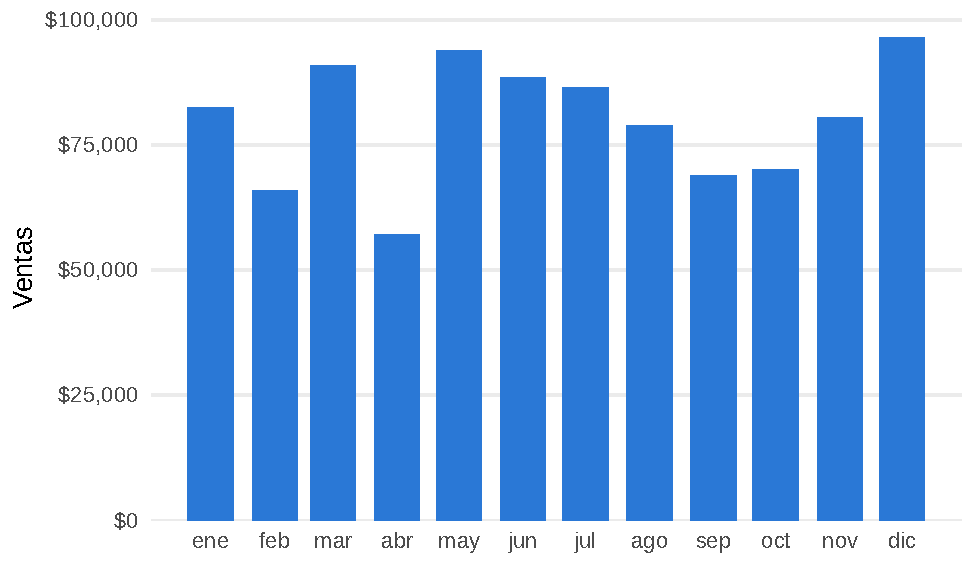
\includegraphics[width=0.9\textwidth]{m06-explorador-mensual}
\caption{Pestaña ``Evolución mensual'' de la app 02 con los filtros por
defecto (salida de \codigo{grafica\_mensual()}).}
\label{fig:m06-explorador-mensual}
\end{figure}

Una sola serie, un solo color, barras que empiezan en cero y eje con
formato de moneda. Se ve que abril fue el mes más flojo y diciembre el más
fuerte. La tabla del top de productos, con el valor por defecto del
deslizador (aquí pedimos 5 para ahorrar espacio):

\begin{rcode}
top_productos(ventas, n = 5)
\end{rcode}
\begin{rsalida}
# A tibble: 5 x 4
  Producto    Categoría  Unidades Ventas    
  <chr>       <chr>         <dbl> <chr>     
1 Producto 06 Juguetes         82 $34,028.04
2 Producto 19 Deportes         85 $28,367.95
3 Producto 31 Alimentos        74 $25,429.70
4 Producto 47 Automotriz       82 $24,527.21
5 Producto 46 Automotriz       74 $24,470.29
\end{rsalida}

El Producto~06 (Juguetes) lidera con \$34,028. Convertimos \codigo{Ventas}
a texto con \codigo{dollar()} al final porque \codigo{renderTable()} muestra
los números tal cual; así el usuario ve ``\$34,028.04'' en vez de
``34028.04''.

\subsection{La interfaz}

Con la lógica lista, la \codigo{ui} solo acomoda piezas. Observa que todas
las opciones salen de los datos (\codigo{opciones\_tienda},
\codigo{min(ventas\$fecha)}\ldots) y que el \codigo{selectizeInput()} usa
\codigo{placeholder = "Todas"} para que el cuadro vacío se lea como ``todas
las categorías''.

\begin{rnoejecutar}[title=app.R (parte 5): interfaz]
ui <- fluidPage(
  titlePanel("Explorador de ventas 2023"),
  sidebarLayout(
    # Barra lateral: todos los filtros juntos
    sidebarPanel(
      width = 3,
      selectInput("tienda", "Tienda:", choices = opciones_tienda),
      selectizeInput("categorias", "Categorías:",
                     choices = opciones_categoria, multiple = TRUE,
                     options = list(placeholder = "Todas")),
      dateRangeInput("fechas", "Periodo:",
                     start = min(ventas$fecha), end = max(ventas$fecha),
                     min = min(ventas$fecha), max = max(ventas$fecha),
                     format = "dd/mm/yyyy", language = "es",
                     separator = " a "),
      radioButtons("metrica", "Medir por:",
                   choices = c("Ventas ($)" = "ventas",
                               "Unidades" = "unidades",
                               "Transacciones" = "transacciones")),
      sliderInput("n_top", "Productos en el top:",
                  min = 5, max = 20, value = 10, step = 5)
    ),
    # Panel principal: resumen arriba y resultados en pestañas
    mainPanel(
      width = 9,
      h4(textOutput("resumen")),
      tabsetPanel(
        tabPanel("Evolución mensual",
                 plotOutput("grafica", height = "380px")),
        tabPanel("Top productos", tableOutput("tabla_top"))
      )
    )
  )
)
\end{rnoejecutar}

\subsection{El servidor}

Gracias a las funciones, el \codigo{server} cabe en una pantalla. Tiene un
único reactivo, \codigo{datos\_filtrados()}, que alimenta las tres salidas
(el grafo de la figura~\ref{fig:m6-grafo}):

\begin{rnoejecutar}[title=app.R (partes 6 y 7): servidor y lanzamiento]
server <- function(input, output, session) {

  # Expresión reactiva: filtra UNA vez y la reutilizan las tres salidas
  datos_filtrados <- reactive({
    req(input$fechas)                      # espera a que haya fechas
    filtrar_ventas(ventas, input$tienda, input$categorias, input$fechas)
  })

  output$resumen <- renderText({
    d <- datos_filtrados()                 # ¡con paréntesis!
    paste0(comma(nrow(d)), " transacciones  |  Ventas: ",
           dollar(sum(d$total_transaccion), accuracy = 1))
  })

  output$grafica <- renderPlot({
    validate(need(nrow(datos_filtrados()) > 0,
                  "No hay ventas con estos filtros. Amplía el periodo."))
    resumir_por_mes(datos_filtrados(), input$metrica) %>%
      grafica_mensual(input$metrica)
  }, res = 96)

  output$tabla_top <- renderTable({
    top_productos(datos_filtrados(), n = input$n_top)
  }, align = "llrr", digits = 0)
}

# 7. Lanzar la app -------------------------------------------------------
shinyApp(ui, server)
\end{rnoejecutar}

Detalles que vale la pena notar:

\begin{itemize}
  \item \codigo{req(input\$fechas)} evita calcular en el instante en que la
        app arranca y el calendario aún no envía su valor.
  \item \codigo{validate(need(...))} muestra un mensaje amable si el
        periodo y los filtros no dejan ninguna venta.
  \item \codigo{renderPlot(\{...\}, res = 96)} dibuja la gráfica con una
        resolución adecuada para pantalla (textos de tamaño normal).
  \item \codigo{renderTable(..., align = "llrr", digits = 0)} alinea a la
        izquierda las dos columnas de texto y a la derecha las numéricas, y
        muestra las unidades sin decimales.
\end{itemize}

\subsection{Probar la app completa con \texorpdfstring{\codigo{testServer()}}{testServer()}}

\codigo{testServer()} también acepta una app completa: le pasas
\codigo{shinyAppDir("carpeta")} y ejecuta su \codigo{app.R} (incluida la
lectura de datos) sin abrir el navegador. Dentro del bloque puedes leer
incluso los reactivos internos, como \codigo{datos\_filtrados()}:

\begin{rcode}
app02 <- shinyAppDir("latex/codigo/apps/02-explorador-ventas")
testServer(app02, {
  session$setInputs(tienda = "Todas", categorias = NULL,
                    fechas = as.Date(c("2023-01-01", "2023-12-31")),
                    metrica = "ventas", n_top = 10)
  print(output$resumen)
  session$setInputs(tienda = "Sucursal Centro",
                    fechas = as.Date(c("2023-07-01", "2023-12-31")))
  print(output$resumen)
  print(range(datos_filtrados()$fecha))       # un reactivo interno
})
\end{rcode}
\begin{rsalida}
[1] "1,000 transacciones  |  Ventas: $959,993"
[1] "46 transacciones  |  Ventas: $49,559"
[1] "2023-07-05" "2023-12-31"
\end{rsalida}

Con todos los filtros por defecto la app resume las 1,000 transacciones
(\$959,993); al pasar a la Sucursal Centro en el segundo semestre quedan
46 transacciones por \$49,559, y el rango de fechas (del 5 de julio al 31
de diciembre) confirma que el filtro funciona. Si algo fallara (una columna mal escrita, un paquete faltante),
lo verías aquí como error, antes de que lo vea tu directora.

\begin{hazlotu}
Abre la app con \codigo{shiny::runApp("latex/codigo/apps/02-explorador-ventas")},
elige ``Sucursal Outlet'', la categoría ``Belleza'' y la métrica
``Unidades''. ¿En qué mes vendió más unidades de belleza el Outlet? Luego
reduce el periodo a una semana de enero y observa el mensaje de
\codigo{validate()}.
\end{hazlotu}

% ----------------------------------------------------------------------------
\section{Dashboards profesionales con shinydashboard}
\label{sec:m6-shinydashboard}

\subsection{Las piezas de \texorpdfstring{\paquete{shinydashboard}}{shinydashboard}}

\paquete{shinydashboard} es un paquete que da a tu app el aspecto clásico
de un tablero de BI: encabezado de color, menú lateral y cajas. Su
estructura siempre es la misma:

\begin{itemize}
  \item \codigo{dashboardPage(header, sidebar, body)}: la página completa,
        con tres argumentos obligatorios en ese orden.
  \item \codigo{dashboardHeader(title = ...)}: la barra superior.
  \item \codigo{dashboardSidebar(...)}: la barra lateral. Suele contener un
        \codigo{sidebarMenu()} con varios \codigo{menuItem()} (las
        ``pestañas'') y, debajo, los filtros globales.
  \item \codigo{dashboardBody(...)}: el cuerpo. Con
        \codigo{tabItems(tabItem(tabName = ...), ...)} defines el contenido
        de cada pestaña; el \codigo{tabName} debe coincidir con el del
        \codigo{menuItem()}.
  \item \codigo{box(title, width, status, ...)}: una caja con título que
        agrupa una gráfica o tabla. \codigo{width} usa la misma cuadrícula de
        12 columnas; \codigo{status = "primary"} le da el color del tema.
  \item \codigo{valueBox(valor, subtitulo, icon, color)}: la tarjeta grande
        de KPI. \codigo{infoBox()} es una variante más compacta con el ícono
        a la izquierda.
\end{itemize}

Un \codigo{valueBox()} también es solo HTML. Imprímelo para ver su
estructura: el valor va en un encabezado grande (\codigo{h3}) y el
subtítulo en un párrafo.

\begin{rcode}
valueBox(value = "$959,993", subtitle = "Ventas totales",
         icon = icon("dollar-sign"), color = "blue", width = 3)
\end{rcode}
\begin{rsalida}
<div class="col-sm-3">
  <div class="small-box bg-blue">
    <div class="inner">
      <h3>$959,993</h3>
      <p>Ventas totales</p>
    </div>
    <div class="icon-large">
      <i class="fas fa-dollar-sign" role="presentation" aria-label="dollar-sign icon"></i>
    </div>
  </div>
</div>
\end{rsalida}

Los íconos vienen de la colección gratuita Font Awesome: busca nombres en
\url{https://fontawesome.com/icons} (por ejemplo \codigo{"store"},
\codigo{"users"}, \codigo{"chart-line"}) y úsalos con \codigo{icon()}.

\begin{consejo}
Resiste la tentación de pintar cada \codigo{valueBox()} de un color
distinto (verde, rojo, amarillo, morado\ldots). En un dashboard el color
debe \emph{significar} algo: usa un mismo color para todas las tarjetas y
reserva el rojo o el verde para cuando un KPI esté por debajo o por encima
de su meta (lo harás en el ejercicio~\ref{ej:m6-3}).
\end{consejo}

% ----------------------------------------------------------------------------
\section{Caso práctico 2: el dashboard ejecutivo}
\label{sec:m6-app03}

\begin{ejemplo}{Dashboard ejecutivo de ventas}
La dirección quiere un tablero con cinco pestañas: \textbf{Resumen} (4 KPIs
y evolución mensual), \textbf{Productos}, \textbf{Tiendas},
\textbf{Clientes} y \textbf{Datos} (tabla con búsqueda y descarga). Los
filtros de periodo, tiendas y categorías deben afectar a todas las pestañas,
y un botón debe regresar todo a su estado inicial. La app está en
\archivo{latex/codigo/apps/03-dashboard-ejecutivo/} y su distribución
aparece en la figura~\ref{fig:m6-maqueta-app03}.
\end{ejemplo}

\begin{figure}[H]
\centering
\begin{tikzpicture}[font=\sffamily\footnotesize,
    zona/.style={draw=gristexto!50, rounded corners=1.5pt, align=center},
    kpi/.style={zona, fill=primario!70, text=white, minimum width=2.25cm,
                minimum height=1.05cm}]
  \draw[gristexto, line width=0.8pt] (0,0) rectangle (13.4,7.6);
  \fill[primario] (0,7) rectangle (3.2,7.6);
  \fill[primario!80] (3.2,7) rectangle (13.4,7.6);
  \node[white, font=\sffamily\bfseries] at (1.6,7.3) {Ventas 2023};
  \node[white] at (3.6,7.3) {$\equiv$};
  % sidebar
  \fill[gray!75!black] (0,0) rectangle (3.2,7);
  \foreach \y/\t in {6.6/Resumen, 6.15/Productos, 5.7/Tiendas, 5.25/Clientes, 4.8/Datos} {
    \node[anchor=west, text=white] at (0.25,\y) {\t};
  }
  \fill[primario!60, opacity=0.6] (0,6.4) rectangle (3.2,6.8);
  \node[anchor=west, text=white, align=left] at (0.2,3.95) {Periodo:\\[1pt]
    \colorbox{white}{\textcolor{black}{01/01/2023 a 31/12/2023}}};
  \node[anchor=west, text=white, align=left] at (0.2,2.95) {Tiendas:\\[1pt]
    \colorbox{white}{\textcolor{black}{\makebox[2.3cm][l]{Todas}}}};
  \node[anchor=west, text=white, align=left] at (0.2,1.95) {Categorías:\\[1pt]
    \colorbox{white}{\textcolor{black}{\makebox[2.3cm][l]{Todas}}}};
  \node[anchor=west, zona, fill=white] at (0.25,1.0) {Quitar filtros};
  % body
  \fill[gray!8] (3.2,0) rectangle (13.4,7);
  \foreach \i/\v/\t in {0/\$959,993/Ventas totales, 1/1{,}000/Transacciones,
                        2/\$960/Ticket promedio, 3/198/Clientes activos} {
    \node[kpi, anchor=north west, align=left] at ({3.4+\i*2.5},6.8)
      {\textbf{\normalsize\v}\\ \t};
  }
  \node[zona, fill=white, minimum width=6.4cm, minimum height=4.2cm,
        anchor=north west] (evo) at (3.4,5.45) {};
  \fill[primario] (3.4,5.45) rectangle (9.8,5.0);
  \node[white, anchor=west] at (3.5,5.22) {Ventas por mes};
  \draw[primario!70, thick] (3.8,3.0) -- (4.3,2.5) -- (4.8,3.2) -- (5.3,2.0)
       -- (5.8,3.3) -- (6.3,3.1) -- (6.8,3.0) -- (7.3,2.8) -- (7.8,2.4)
       -- (8.3,2.45) -- (8.8,2.9) -- (9.3,3.45);
  \fill[acento] (9.3,3.45) circle (0.08);
  \node[zona, fill=white, minimum width=3.4cm, minimum height=4.2cm,
        anchor=north west] at (9.85,5.45) {};
  \fill[primario] (9.85,5.45) rectangle (13.25,5.0);
  \node[white, anchor=west, font=\sffamily\scriptsize] at (9.9,5.22) {Ventas por método de pago};
  \foreach \y/\w in {4.4/2.6, 3.8/2.2, 3.2/2.0, 2.6/0.9} {
    \fill[primario!70] (10.2,\y) rectangle ++(\w,0.35);
  }
  \node[text=gristexto] at (8.3,0.6) {\codigo{box(width = 8)} \hspace{1.6cm} \codigo{box(width = 4)}};
  \node[text=acento, anchor=south] at (8.3,6.85) {};
\end{tikzpicture}
\caption{Maqueta de la pestaña ``Resumen'' de la app 03: menú y filtros en
la barra lateral, cuatro \codigo{valueBox()} arriba y dos \codigo{box()} con
gráficas.}
\label{fig:m6-maqueta-app03}
\end{figure}

La app tiene dos archivos:

\begin{textocodigo}
03-dashboard-ejecutivo/
|-- app.R                      <- interfaz y servidor
+-- R/
    +-- funciones_dashboard.R  <- datos, KPIs, gráficas y tablas
\end{textocodigo}

Shiny tiene una regla muy útil: \textbf{antes de ejecutar \archivo{app.R},
carga automáticamente todos los archivos \archivo{.R} de la subcarpeta
\archivo{R/}}. Así la lógica vive en su propio archivo y \archivo{app.R} se
queda con lo visual. Vamos a recorrer primero las funciones (que sí podemos
ejecutar y probar aquí) y después la app.

\subsection{Cargar y unir los datos}

\codigo{cargar\_datos\_dashboard()} lee cuatro CSV, se queda con las
columnas necesarias y los une a las transacciones con los \emph{joins} del
Módulo~\ref{cap:manipulacion}. El resultado es una sola tabla ``ancha'' con
todo lo que el dashboard necesita:

\begin{rcode}
# ---- Colores y tema corporativos ---------------------------------------
color_principal <- "#2a78d6"   # una sola serie
color_resalte   <- "#eb6834"   # para destacar un elemento
color_gris      <- "#b5b3ad"   # el resto, cuando se resalta uno
paleta_libro <- c("#2a78d6", "#eb6834", "#1baf7a", "#eda100",
                  "#e87ba4", "#008300", "#4a3aa7", "#e34948")

tema_dashboard <- function(base_size = 12) {
  theme_minimal(base_size = base_size) +
    theme(panel.grid.minor = element_blank(),
          legend.position  = "top",
          plot.margin      = margin(5, 15, 5, 5))  # aire a la derecha
}

cargar_datos_dashboard <- function(carpeta = buscar_datasets()) {
  leer <- function(archivo) {
    read_csv(file.path(carpeta, archivo), show_col_types = FALSE)
  }
  productos <- leer("productos.csv") %>%
    select(producto_id, nombre_producto, categoria, costo)
  tiendas <- leer("tiendas.csv") %>%
    transmute(tienda_id, ciudad,
              tienda = sub("Sucursal ", "", nombre_tienda))  # nombre corto
  clientes <- leer("clientes.csv") %>%
    select(cliente_id, nombre_cliente = nombre, segmento, es_premium)

  leer("transacciones.csv") %>%
    left_join(productos, by = "producto_id") %>%
    left_join(tiendas,   by = "tienda_id") %>%
    left_join(clientes,  by = "cliente_id") %>%
    mutate(mes = floor_date(fecha, "month"),
           segmento = factor(segmento, levels = c("Joven", "Adulto",
                                                  "Maduro", "Senior"))) %>%
    select(transaccion_id, fecha, mes, tienda, ciudad, categoria,
           producto_id, nombre_producto, cliente_id, nombre_cliente,
           segmento, es_premium, metodo_pago, cantidad, precio_venta,
           costo, total_transaccion)
}

datos <- cargar_datos_dashboard()
glimpse(datos)
\end{rcode}
\begin{rsalida}
Rows: 1,000
Columns: 17
$ transaccion_id    <dbl> 1, 2, 3, 4, 5, 6, 7, 8, 9, 10, 11, 12, 13,~
$ fecha             <date> 2023-01-13, 2023-01-09, 2023-02-20, 2023-~
$ mes               <date> 2023-01-01, 2023-01-01, 2023-02-01, 2023-~
$ tienda            <chr> "Express", "Norte", "Plaza B", "Plaza A", ~
$ ciudad            <chr> "Querétaro", "Guadalajara", "Guadalajara",~
$ categoria         <chr> "Automotriz", "Automotriz", "Juguetes", "D~
$ producto_id       <dbl> 3, 47, 6, 17, 28, 46, 30, 48, 21, 12, 49, ~
$ nombre_producto   <chr> "Producto 03", "Producto 47", "Producto 06~
$ cliente_id        <dbl> 155, 155, 75, 51, 173, 135, 90, 168, 13, 9~
$ nombre_cliente    <chr> "Marta González", "Marta González", "Diego~
$ segmento          <fct> Adulto, Adulto, Maduro, Senior, Maduro, Ma~
$ es_premium        <lgl> TRUE, TRUE, FALSE, FALSE, FALSE, TRUE, FAL~
$ metodo_pago       <chr> "Tarjeta Crédito", "Tarjeta Débito", "Tarj~
$ cantidad          <dbl> 4, 4, 3, 4, 1, 2, 4, 2, 2, 5, 2, 3, 4, 2, ~
$ precio_venta      <dbl> 303.97, 58.07, 275.46, 105.28, 205.47, 534~
$ costo             <dbl> 294.30, 55.00, 84.55, 156.61, 17.23, 177.5~
$ total_transaccion <dbl> 1215.88, 232.28, 826.38, 421.12, 205.47, 1~
\end{rsalida}

1,000 filas y 17 columnas: cada transacción ya trae el nombre corto de su
tienda, la categoría y el costo del producto, y el segmento del cliente.
(Usamos \codigo{sub("Sucursal ", "", nombre\_tienda)} para mostrar
``Centro'' en lugar de ``Sucursal Centro'' y ahorrar espacio en las
gráficas.) La función \codigo{buscar\_datasets()} de este archivo es la
misma de la sección~\ref{sec:m6-rutas}.

\subsection{Filtros globales y KPIs}

\begin{rcode}
# ---- Filtros globales --------------------------------------------------
# Vacío (NULL o character(0)) significa "todas".
filtrar_datos <- function(datos, fechas, tiendas = NULL,
                          categorias = NULL) {
  datos <- filter(datos, fecha >= fechas[1], fecha <= fechas[2])
  if (length(tiendas) > 0) {
    datos <- filter(datos, tienda %in% tiendas)
  }
  if (length(categorias) > 0) {
    datos <- filter(datos, categoria %in% categorias)
  }
  datos
}

calcular_kpis <- function(datos) {
  datos %>%
    summarise(
      ventas          = sum(total_transaccion),
      transacciones   = n(),
      ticket_promedio = ventas / transacciones,
      unidades        = sum(cantidad),
      clientes        = n_distinct(cliente_id),
      pct_premium     = mean(es_premium[!duplicated(cliente_id)]),
      compras_cliente = transacciones / clientes
    )
}

# Formatos para mostrar los KPIs como texto ("--" si no hay dato)
formato_pesos <- function(x) {
  if_else(is.na(x), "--", dollar(x, accuracy = 1))
}
formato_numero <- function(x, decimales = 0) {
  if_else(is.na(x), "--", comma(x, accuracy = 10^-decimales))
}
formato_pct <- function(x) {
  if_else(is.na(x), "--", percent(x, accuracy = 0.1))
}
\end{rcode}

Dos detalles de negocio en \codigo{calcular\_kpis()}: los \emph{clientes
activos} se cuentan con \codigo{n\_distinct()} (un cliente que compró cinco
veces cuenta una vez), y el \% de clientes premium se calcula sobre
clientes únicos (\codigo{!duplicated(cliente\_id)}), no sobre
transacciones. Las funciones de formato devuelven \codigo{"-{}-"} cuando no
hay dato (por ejemplo, el ticket promedio de un filtro sin ventas), en lugar
de un feo \codigo{NA}.

\begin{rcode}
anio <- as.Date(c("2023-01-01", "2023-12-31"))
kpis_total <- calcular_kpis(filtrar_datos(datos, anio))
kpis_total %>% select(ventas, transacciones, ticket_promedio, clientes)
formato_pesos(kpis_total$ventas)
formato_pct(kpis_total$pct_premium)

# Los mismos KPIs para dos tiendas y una categoría, primer semestre
filtrar_datos(datos, as.Date(c("2023-01-01", "2023-06-30")),
              tiendas = c("Centro", "Norte"),
              categorias = "Electrónica") %>%
  calcular_kpis() %>%
  select(ventas, transacciones, ticket_promedio, clientes)
\end{rcode}
\begin{rsalida}
# A tibble: 1 x 4
   ventas transacciones ticket_promedio clientes
    <dbl>         <int>           <dbl>    <int>
1 959993.          1000            960.      198
[1] "$959,993"
[1] "36.4%"
# A tibble: 1 x 4
  ventas transacciones ticket_promedio clientes
   <dbl>         <int>           <dbl>    <int>
1  6937.            10            694.       10
\end{rsalida}

En todo 2023 hubo 1,000 transacciones por \$959,993, con un ticket
promedio de \$960 y 198 de los 200 clientes activos; el 36.4\% de esos
clientes es premium. Con los filtros del segundo ejemplo la historia cambia
por completo: solo 10 transacciones de Electrónica entre Centro y Norte en el
primer semestre. Estas cifras son exactamente las que mostrarán los
\codigo{valueBox()}.

\subsection{Las gráficas de cada pestaña}

Cada gráfica es una función que recibe los datos \emph{ya filtrados} y
devuelve un objeto \codigo{ggplot}. Todas usan el tema del dashboard y los
colores corporativos del Módulo~\ref{cap:visualizacion}.

\begin{rcode}
grafica_evolucion <- function(datos) {
  por_mes <- datos %>%
    group_by(mes) %>%
    summarise(ventas = sum(total_transaccion), .groups = "drop")
  mejor_mes <- slice_max(por_mes, ventas, n = 1, with_ties = FALSE)
  ggplot(por_mes, aes(x = mes, y = ventas)) +
    geom_line(color = color_principal, linewidth = 0.8) +
    geom_point(color = color_principal, size = 2) +
    geom_point(data = mejor_mes, color = color_resalte, size = 3.5) +
    geom_text(data = mejor_mes, aes(label = dollar(ventas, accuracy = 1)),
              vjust = -1.2, size = 3.5, color = "gray25") +
    scale_x_date(date_labels = "%b", date_breaks = "1 month") +
    scale_y_continuous(labels = label_dollar(), limits = c(0, NA),
                       expand = expansion(mult = c(0, 0.15))) +
    labs(x = NULL, y = "Ventas") +
    tema_dashboard()
}

p_evolucion <- grafica_evolucion(datos)
p_evolucion
\end{rcode}

\begin{figure}[H]
\centering
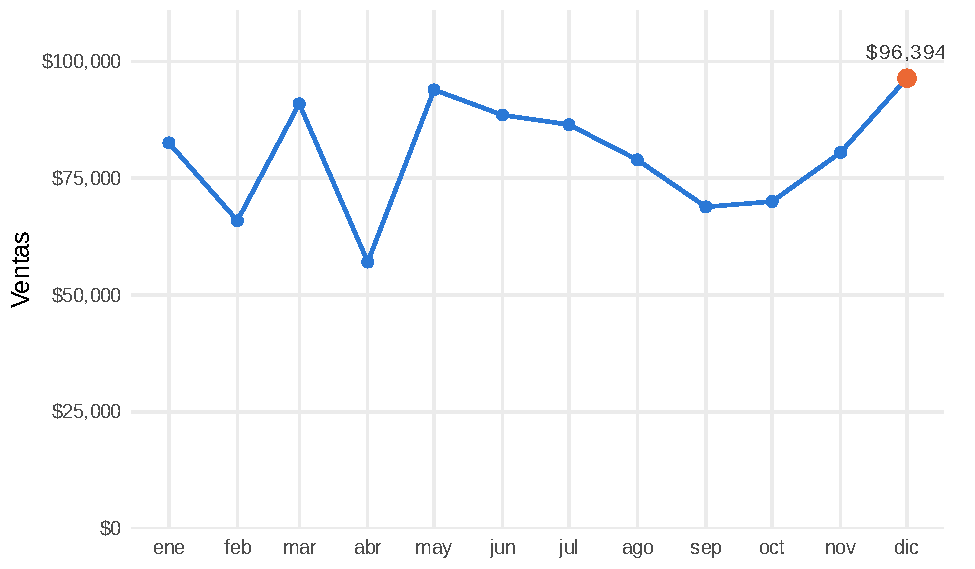
\includegraphics[width=0.9\textwidth]{m06-evolucion}
\caption{Pestaña Resumen: ventas por mes con el mejor mes resaltado
(\codigo{grafica\_evolucion()}).}
\label{fig:m06-evolucion}
\end{figure}

La línea usa un solo color y solo el mejor mes lleva color de resalte y
etiqueta (diciembre, con \$96,394): el ojo va directo a lo importante. Como
el eje Y empieza en cero, la caída de abril se ve en su verdadera magnitud.

\begin{rcode}
grafica_metodo_pago <- function(datos) {
  datos %>%
    group_by(metodo_pago) %>%
    summarise(ventas = sum(total_transaccion), .groups = "drop") %>%
    mutate(participacion = ventas / sum(ventas)) %>%
    ggplot(aes(x = participacion,
               y = reorder(metodo_pago, participacion))) +
    geom_col(fill = color_principal, width = 0.7) +
    scale_x_continuous(labels = label_percent(),
                       expand = expansion(mult = c(0, 0.05))) +
    labs(x = "% de las ventas", y = NULL) +
    tema_dashboard()
}

grafica_barras <- function(resumen, etiqueta_y = NULL) {
  # resumen: columnas 'nombre' y 'ventas'; barras horizontales ordenadas
  ggplot(resumen, aes(x = ventas, y = reorder(nombre, ventas))) +
    geom_col(fill = color_principal, width = 0.7) +
    scale_x_continuous(labels = label_dollar(),
                       expand = expansion(mult = c(0, 0.05))) +
    labs(x = "Ventas", y = etiqueta_y) +
    tema_dashboard()
}

grafica_top_productos <- function(datos, n = 10) {
  datos %>%
    group_by(nombre = nombre_producto) %>%
    summarise(ventas = sum(total_transaccion), .groups = "drop") %>%
    slice_max(ventas, n = n, with_ties = FALSE) %>%
    grafica_barras()
}

grafica_categorias <- function(datos) {
  datos %>%
    group_by(nombre = categoria) %>%
    summarise(ventas = sum(total_transaccion), .groups = "drop") %>%
    grafica_barras()
}

p_top <- grafica_top_productos(datos)
p_top
\end{rcode}

\codigo{grafica\_barras()} es una función ``genérica'' que reutilizan la
gráfica de productos y la de categorías: ambas resumen a dos columnas,
\codigo{nombre} y \codigo{ventas}, y le pasan el resultado. Escribir la
gráfica una sola vez garantiza que las dos pestañas se vean iguales
(figura~\ref{fig:m06-top-productos}).

\begin{figure}[H]
\centering
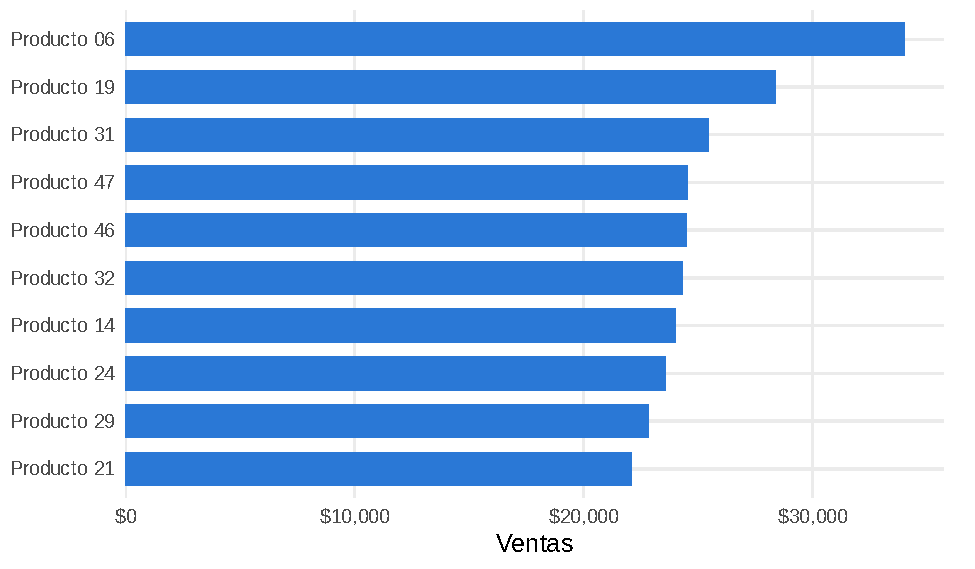
\includegraphics[width=0.9\textwidth]{m06-top-productos}
\caption{Pestaña Productos: los 10 productos con más ventas
(\codigo{grafica\_top\_productos()}).}
\label{fig:m06-top-productos}
\end{figure}

\begin{rcode}
grafica_tiendas <- function(datos) {
  por_tienda <- datos %>%
    group_by(tienda) %>%
    summarise(ventas = sum(total_transaccion), .groups = "drop") %>%
    mutate(es_mejor = ventas == max(ventas))    # la tienda líder
  ggplot(por_tienda, aes(x = ventas, y = reorder(tienda, ventas),
                         fill = es_mejor)) +
    geom_col(width = 0.7) +
    geom_text(data = filter(por_tienda, es_mejor),
              aes(label = dollar(ventas, accuracy = 1)),
              hjust = 1.1, color = "white", size = 3.5) +
    scale_fill_manual(values = c(`TRUE` = color_resalte,
                                 `FALSE` = color_gris), guide = "none") +
    scale_x_continuous(labels = label_dollar(),
                       expand = expansion(mult = c(0, 0.05))) +
    labs(x = "Ventas", y = NULL) +
    tema_dashboard()
}

p_tiendas <- grafica_tiendas(datos)
p_tiendas
\end{rcode}

\begin{figure}[H]
\centering
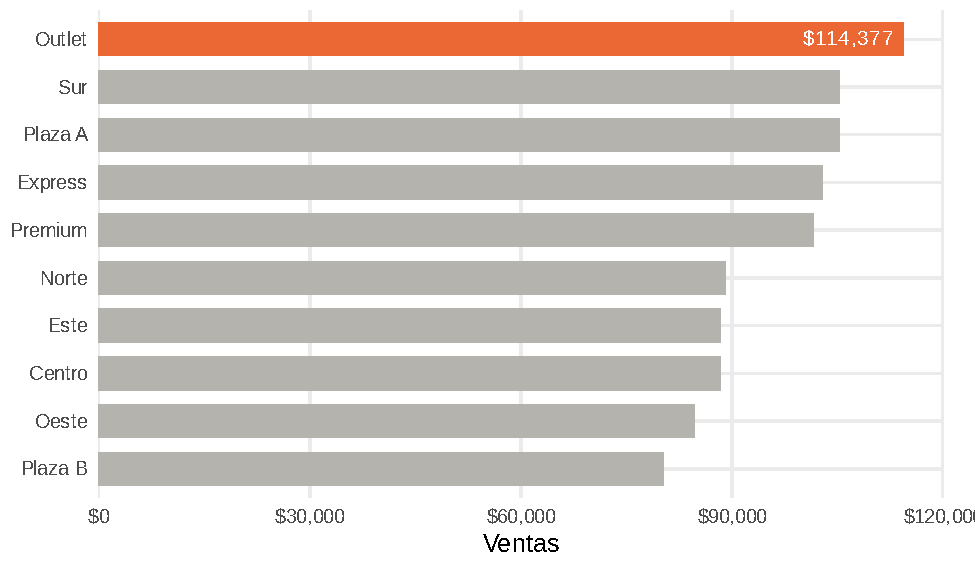
\includegraphics[width=0.9\textwidth]{m06-tiendas}
\caption{Pestaña Tiendas: la tienda líder en color de resalte y el resto en
gris (\codigo{grafica\_tiendas()}).}
\label{fig:m06-tiendas}
\end{figure}

La figura~\ref{fig:m06-tiendas} aplica la técnica de ``resaltar uno y
agrisar el resto'': la pregunta es ``¿quién lidera?'' y la respuesta salta a
la vista. Un hallazgo interesante: el \emph{Outlet}, una de las tiendas más
pequeñas (350 m$^2$), es la que más vende en estos datos simulados, con
\$114,377.

\begin{rcode}
grafica_segmentos <- function(datos) {
  datos %>%
    mutate(tipo = if_else(es_premium, "Premium", "Regular")) %>%
    group_by(segmento, tipo) %>%
    summarise(ventas = sum(total_transaccion), .groups = "drop") %>%
    ggplot(aes(x = segmento, y = ventas, fill = tipo)) +
    geom_col(position = position_dodge(width = 0.8), width = 0.7) +
    scale_fill_manual(values = c(Premium = paleta_libro[2],
                                 Regular = paleta_libro[1])) +
    scale_y_continuous(labels = label_dollar(),
                       expand = expansion(mult = c(0, 0.05))) +
    labs(x = "Segmento de edad", y = "Ventas", fill = "Tipo de cliente") +
    tema_dashboard()
}

p_segmentos <- grafica_segmentos(datos)
p_segmentos
\end{rcode}

\begin{figure}[H]
\centering
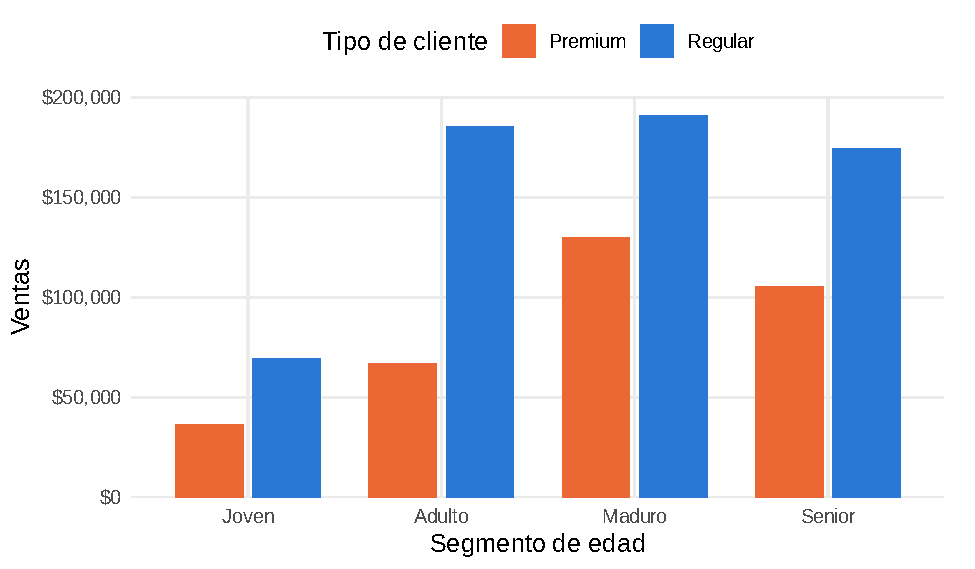
\includegraphics[width=0.9\textwidth]{m06-segmentos}
\caption{Pestaña Clientes: ventas por segmento de edad y tipo de cliente
(\codigo{grafica\_segmentos()}).}
\label{fig:m06-segmentos}
\end{figure}

Aquí sí hay dos series (Premium y Regular), así que usamos dos colores de la
paleta y leyenda. En todos los segmentos los clientes regulares aportan más
ventas que los premium, lo cual es lógico porque son cerca del 64\% de los
clientes.

\subsection{Tablas y detalle}

\begin{rcode}
# ---- Tablas ------------------------------------------------------------
tabla_tiendas <- function(datos) {
  datos %>%
    group_by(Tienda = tienda) %>%
    summarise(Ventas = sum(total_transaccion),
              Transacciones = n(),
              Ticket = Ventas / Transacciones, .groups = "drop") %>%
    arrange(desc(Ventas)) %>%
    mutate(Ventas = formato_pesos(Ventas), Ticket = formato_pesos(Ticket))
}

tabla_top_clientes <- function(datos, n = 10) {
  datos %>%
    group_by(Cliente = nombre_cliente, Segmento = segmento) %>%
    summarise(Compras = n(), Ventas = sum(total_transaccion),
              .groups = "drop") %>%
    slice_max(Ventas, n = n, with_ties = FALSE) %>%
    mutate(Ventas = formato_pesos(Ventas))
}

# Datos listos para la tabla interactiva y para las descargas
datos_detalle <- function(datos) {
  datos %>%
    arrange(fecha, transaccion_id) %>%
    select(Fecha = fecha, Tienda = tienda, `Categoría` = categoria,
           Producto = nombre_producto, Cliente = nombre_cliente,
           Cantidad = cantidad, Precio = precio_venta,
           Total = total_transaccion, `Método de pago` = metodo_pago)
}

tabla_tiendas(datos) %>% head(4)
tabla_top_clientes(datos, n = 3)
\end{rcode}
\begin{rsalida}
# A tibble: 4 x 4
  Tienda  Ventas   Transacciones Ticket
  <chr>   <chr>            <int> <chr> 
1 Outlet  $114,377           106 $1,079
2 Sur     $105,305           109 $966  
3 Plaza A $105,216           109 $965  
4 Express $102,791           108 $952  
# A tibble: 3 x 4
  Cliente        Segmento Compras Ventas 
  <chr>          <fct>      <int> <chr>  
1 Luis Hernández Maduro        18 $15,744
2 Pedro Cruz     Adulto        13 $14,680
3 Miguel Flores  Adulto        11 $13,742
\end{rsalida}

El Outlet no solo vende más: también tiene el ticket promedio más alto
(\$1,079). Las funciones que preparan la tabla interactiva
(\codigo{tabla\_detalle\_dt()}) las veremos en la
sección~\ref{sec:m6-dt}.

\subsection{La interfaz del dashboard}

Con la lógica probada, pasamos a \archivo{app.R}. Primero paquetes y datos
(fuera del \codigo{server}, una sola vez) y luego encabezado y barra
lateral:

\begin{rnoejecutar}[title=app.R (partes 1 a 3)]
# 1. Paquetes ------------------------------------------------------------
library(shiny)
library(shinydashboard)   # dashboardPage(), box(), valueBox()...
library(dplyr)
library(readr)
library(ggplot2)
library(lubridate)
library(scales)
library(DT)               # tablas interactivas
library(writexl)          # descarga en Excel

# 2. Datos: se leen UNA vez, fuera del server ----------------------------
datos <- cargar_datos_dashboard()
fecha_min <- min(datos$fecha)
fecha_max <- max(datos$fecha)
opciones_tiendas    <- sort(unique(datos$tienda))
opciones_categorias <- sort(unique(datos$categoria))

# 3. Interfaz: encabezado y barra lateral --------------------------------
encabezado <- dashboardHeader(title = "Ventas 2023")

barra_lateral <- dashboardSidebar(
  sidebarMenu(
    id = "menu",
    menuItem("Resumen",   tabName = "resumen",   icon = icon("gauge")),
    menuItem("Productos", tabName = "productos", icon = icon("box")),
    menuItem("Tiendas",   tabName = "tiendas",   icon = icon("store")),
    menuItem("Clientes",  tabName = "clientes",  icon = icon("users")),
    menuItem("Datos",     tabName = "datos",     icon = icon("table"))
  ),
  # Filtros globales: afectan a TODAS las pestañas
  dateRangeInput("fechas", "Periodo:", start = fecha_min, end = fecha_max,
                 min = fecha_min, max = fecha_max, format = "dd/mm/yyyy",
                 language = "es", separator = " a "),
  selectizeInput("tiendas", "Tiendas:", choices = opciones_tiendas,
                 multiple = TRUE, options = list(placeholder = "Todas")),
  selectizeInput("categorias", "Categorías:",
                 choices = opciones_categorias, multiple = TRUE,
                 options = list(placeholder = "Todas")),
  actionButton("limpiar", "Quitar filtros", icon = icon("rotate-left"))
)
\end{rnoejecutar}

Los filtros van \emph{después} del \codigo{sidebarMenu()}, dentro de
\codigo{dashboardSidebar()}: así quedan visibles en todas las pestañas, lo
que deja claro que son globales. Los \codigo{selectizeInput()} múltiples
usan el marcador ``Todas'' para indicar que vacío significa sin filtro.

El cuerpo tiene un \codigo{tabItem()} por cada \codigo{menuItem()}. Cada
fila es un \codigo{fluidRow()} y cada gráfica vive en una \codigo{box()}:

\begin{rnoejecutar}[title=app.R (parte 4): cuerpo]
# 4. Interfaz: cuerpo con una tabItem por pestaña del menú ---------------
cuerpo <- dashboardBody(
  tabItems(
    tabItem(tabName = "resumen",
      fluidRow(                                   # fila de KPIs arriba
        valueBoxOutput("kpi_ventas", width = 3),
        valueBoxOutput("kpi_transacciones", width = 3),
        valueBoxOutput("kpi_ticket", width = 3),
        valueBoxOutput("kpi_clientes", width = 3)
      ),
      fluidRow(
        box(title = "Ventas por mes", width = 8, status = "primary",
            solidHeader = TRUE, plotOutput("graf_evolucion", height = 300)),
        box(title = "Ventas por método de pago", width = 4,
            status = "primary", solidHeader = TRUE,
            plotOutput("graf_pago", height = 300))
      )
    ),
    tabItem(tabName = "productos",
      fluidRow(
        box(title = "Top 10 productos", width = 6, status = "primary",
            plotOutput("graf_top_productos", height = 380)),
        box(title = "Ventas por categoría", width = 6, status = "primary",
            plotOutput("graf_categorias", height = 380))
      )
    ),
    tabItem(tabName = "tiendas",
      fluidRow(
        box(title = "Ventas por tienda", width = 7, status = "primary",
            plotOutput("graf_tiendas", height = 380)),
        box(title = "Indicadores por tienda", width = 5,
            status = "primary", tableOutput("tabla_tiendas"))
      )
    ),
    tabItem(tabName = "clientes",
      fluidRow(
        infoBoxOutput("info_clientes"),
        infoBoxOutput("info_premium"),
        infoBoxOutput("info_frecuencia")
      ),
      fluidRow(
        box(title = "Ventas por segmento", width = 6, status = "primary",
            plotOutput("graf_segmentos", height = 320)),
        box(title = "Top 10 clientes", width = 6, status = "primary",
            tableOutput("tabla_clientes"))
      )
    ),
    tabItem(tabName = "datos",
      fluidRow(
        box(title = "Detalle de transacciones", width = 12,
            status = "primary",
            downloadButton("descargar_csv", "Descargar CSV"),
            downloadButton("descargar_excel", "Descargar Excel"),
            br(), br(),
            DTOutput("tabla_detalle"))
      )
    )
  )
)

ui <- dashboardPage(encabezado, barra_lateral, cuerpo, skin = "blue")
\end{rnoejecutar}

Observa la fila de KPIs: cuatro \codigo{valueBoxOutput()} de ancho 3 suman
exactamente 12 columnas. En la pestaña Clientes, los \codigo{infoBoxOutput()}
tienen el ancho por defecto (4), así que caben tres por fila.

\subsection{El servidor del dashboard}

\begin{rnoejecutar}[title=app.R (parte 5): reactivos, botón y KPIs]
# 5. Servidor: datos filtrados, KPIs y botón para limpiar filtros --------
server <- function(input, output, session) {

  # La pieza central: TODO lo demás depende de datos_filtrados()
  datos_filtrados <- reactive({
    req(input$fechas)
    filtrar_datos(datos, input$fechas, input$tiendas, input$categorias)
  }) %>%
    bindCache(input$fechas, input$tiendas, input$categorias)

  kpis <- reactive(calcular_kpis(datos_filtrados()))

  # Igual que datos_filtrados(), pero si los filtros no dejan ninguna
  # venta, las salidas que lo usan muestran un mensaje amable
  datos_validos <- reactive({
    validate(need(nrow(datos_filtrados()) > 0,
                  "No hay ventas con estos filtros."))
    datos_filtrados()
  })

  observeEvent(input$limpiar, {
    updateDateRangeInput(session, "fechas", start = fecha_min,
                         end = fecha_max)
    updateSelectizeInput(session, "tiendas", selected = character(0))
    updateSelectizeInput(session, "categorias", selected = character(0))
  })

  output$kpi_ventas <- renderValueBox({
    valueBox(formato_pesos(kpis()$ventas), "Ventas totales",
             icon = icon("dollar-sign"), color = "blue")
  })
  output$kpi_transacciones <- renderValueBox({
    valueBox(formato_numero(kpis()$transacciones), "Transacciones",
             icon = icon("receipt"), color = "blue")
  })
  output$kpi_ticket <- renderValueBox({
    valueBox(formato_pesos(kpis()$ticket_promedio), "Ticket promedio",
             icon = icon("cart-shopping"), color = "blue")
  })
  output$kpi_clientes <- renderValueBox({
             icon = icon("users"), color = "blue")
  })
\end{rnoejecutar}

La arquitectura reactiva es la de la figura~\ref{fig:m6-grafo}, un poco más
grande: \codigo{datos\_filtrados()} depende de los tres filtros; de él
cuelgan \codigo{kpis()} (que alimenta los \codigo{valueBox()} y los
\codigo{infoBox()}) y \codigo{datos\_validos()} (que alimenta las gráficas y
muestra un mensaje si no hay ventas). El botón ``Quitar filtros'' es un
\codigo{observeEvent()} que devuelve cada entrada a su valor inicial con las
funciones \codigo{update...()}. Sobre \codigo{bindCache()} hablaremos en la
sección~\ref{sec:m6-buenas-practicas}.

\begin{rnoejecutar}[title=app.R (partes 6 a 8): salidas, descargas y lanzamiento]
  # 6. Servidor: gráficas y tablas de cada pestaña -----------------------
  output$graf_evolucion <- renderPlot({
    grafica_evolucion(datos_validos())
  }, res = 96)
  output$graf_pago <- renderPlot({
    grafica_metodo_pago(datos_validos())
  }, res = 96)
  output$graf_top_productos <- renderPlot({
    grafica_top_productos(datos_validos())
  }, res = 96)
  output$graf_categorias <- renderPlot({
    grafica_categorias(datos_validos())
  }, res = 96)
  output$graf_tiendas <- renderPlot({
    grafica_tiendas(datos_validos())
  }, res = 96)
  output$tabla_tiendas <- renderTable(tabla_tiendas(datos_filtrados()))

  output$info_clientes <- renderInfoBox({
    infoBox("Clientes activos", formato_numero(kpis()$clientes),
            icon = icon("users"), color = "blue")
  })
  output$info_premium <- renderInfoBox({
    infoBox("Clientes premium", formato_pct(kpis()$pct_premium),
            icon = icon("star"), color = "blue")
  })
  output$info_frecuencia <- renderInfoBox({
    infoBox("Compras por cliente",
            formato_numero(kpis()$compras_cliente, decimales = 1),
            icon = icon("repeat"), color = "blue")
  })
  output$graf_segmentos <- renderPlot({
    grafica_segmentos(datos_validos())
  }, res = 96)
  output$tabla_clientes <- renderTable(
    tabla_top_clientes(datos_filtrados()))

  output$tabla_detalle <- renderDT(tabla_detalle_dt(datos_filtrados()))

  # 7. Servidor: descargas (respetan los filtros activos) ----------------
  output$descargar_csv <- downloadHandler(
    filename = function() paste0("ventas_filtradas_", Sys.Date(), ".csv"),
    content  = function(file) {
      write_excel_csv(datos_detalle(datos_filtrados()), file)
    }
  )
  output$descargar_excel <- downloadHandler(
    filename = function() paste0("ventas_filtradas_", Sys.Date(), ".xlsx"),
    content  = function(file) {
      write_xlsx(datos_detalle(datos_filtrados()), file)
    }
  )
}

# 8. Lanzar la app -------------------------------------------------------
shinyApp(ui, server)
\end{rnoejecutar}

Cada \codigo{renderPlot()} tiene una sola línea: llama a su función con los
datos válidos. Si mañana cambias el diseño de una gráfica, lo haces en
\archivo{R/funciones\_dashboard.R} sin tocar \archivo{app.R}.

\subsection{Probar el dashboard completo}

\begin{rcode}
app03 <- shinyAppDir("latex/codigo/apps/03-dashboard-ejecutivo")
testServer(app03, {
  session$setInputs(fechas = as.Date(c("2023-01-01", "2023-12-31")),
                    tiendas = NULL, categorias = NULL)
  cat("Ventas:", kpis()$ventas, "| Clientes:", kpis()$clientes, "\n")

  # El usuario elige dos tiendas y una categoría
  session$setInputs(tiendas = c("Centro", "Norte"),
                    categorias = "Electrónica")
  cat("Ventas:", round(kpis()$ventas, 2),
      "| Transacciones:", kpis()$transacciones, "\n")

  # Filtros sin ventas: las gráficas muestran el mensaje de validate()
  session$setInputs(tiendas = "Express", categorias = "Ropa",
                    fechas = as.Date(c("2023-01-01", "2023-01-31")))
  tryCatch(output$graf_evolucion,
           error = function(e) cat("Gráfica:", conditionMessage(e), "\n"))
  cat("Ticket en el valueBox:", formato_pesos(kpis()$ticket_promedio), "\n")
})
\end{rcode}
\begin{rsalida}
Ventas: 959992.7 | Clientes: 198 
Ventas: 32911.76 | Transacciones: 31 
Gráfica: No hay ventas con estos filtros. 
Ticket en el valueBox: -- 
\end{rsalida}

La prueba confirma los tres escenarios: todo el año (\$959,992.70 y 198
clientes), un filtro combinado (31 transacciones) y un filtro sin ventas,
donde la gráfica muestra el mensaje amable y la tarjeta del ticket muestra
``-{}-'' en lugar de \codigo{NA}.

\begin{hazlotu}
Ejecuta \codigo{shiny::runApp("latex/codigo/apps/03-dashboard-ejecutivo")}.
Recorre las cinco pestañas; luego elige solo la tienda ``Outlet'' y
comprueba que \emph{todas} las pestañas cambian. Pulsa ``Quitar filtros''.
¿Qué método de pago concentra más ventas en el Outlet?
\end{hazlotu}

% ----------------------------------------------------------------------------
\section{Descargas, tablas interactivas y gráficas interactivas}
\label{sec:m6-descargas}

\subsection{Botones de descarga con \texorpdfstring{\codigo{downloadHandler()}}{downloadHandler()}}

Lo primero que pide cualquier usuario de un dashboard es ``¿me lo puedes
pasar en Excel?''. Un botón de descarga tiene, como toda salida, dos mitades:
\codigo{downloadButton("id", "Texto")} en la \codigo{ui} y
\codigo{output\$id <- downloadHandler(filename, content)} en el
\codigo{server}:

\begin{itemize}
  \item \codigo{filename}: una \emph{función} que devuelve el nombre del
        archivo. Incluir la fecha (\codigo{Sys.Date()}) evita que el usuario
        sobrescriba descargas anteriores.
  \item \codigo{content}: una \emph{función} que recibe una ruta temporal
        (\codigo{file}) y escribe ahí el archivo. Shiny se encarga de
        enviarlo al navegador.
\end{itemize}

En la app 03 (parte 7 del servidor) hay dos botones, uno para CSV y otro
para Excel, y ambos descargan \codigo{datos\_detalle(datos\_filtrados())}:
\textbf{respetan los filtros activos}, que es lo que el usuario espera.
Para el CSV usamos \codigo{write\_excel\_csv()} de \paquete{readr} en lugar
de \codigo{write\_csv()}: agrega una marca invisible al inicio del archivo
para que Excel muestre bien los acentos (``Categoría'', ``Tarjeta
Crédito''). Para Excel usamos \codigo{write\_xlsx()} de \paquete{writexl}.

Como \codigo{content} es una función normal, puedes probar lo que hará
escribiendo tú mismo los archivos:

\begin{rcode}
library(writexl)
dir.create("resultados", showWarnings = FALSE)
detalle <- datos_detalle(filtrar_datos(datos, anio, tiendas = "Outlet"))
write_excel_csv(detalle, "resultados/ventas_outlet.csv")
write_xlsx(detalle, "resultados/ventas_outlet.xlsx")
dim(detalle)
names(detalle)
\end{rcode}
\begin{rsalida}
[1] 106   9
[1] "Fecha"          "Tienda"         "Categoría"     
[4] "Producto"       "Cliente"        "Cantidad"      
[7] "Precio"         "Total"          "Método de pago"
\end{rsalida}

Las 106 transacciones del Outlet, con 9 columnas de nombres legibles, listas
para quien las pida. En la prueba con \codigo{testServer()} también puedes
leer \codigo{output\$descargar\_csv}: devuelve la ruta del archivo generado,
que puedes abrir con \codigo{read\_csv()} para comprobar su contenido.

\subsection{Tablas interactivas con \texorpdfstring{\paquete{DT}}{DT}}
\label{sec:m6-dt}

\codigo{renderTable()} está bien para tablas pequeñas (un top 10). Para
mostrar cientos o miles de filas necesitas búsqueda, orden por columna y
paginación: eso hace \paquete{DT}, un puente a la biblioteca DataTables de
JavaScript. La pareja es \codigo{DTOutput()} / \codigo{renderDT()}, y
dentro se usa \codigo{datatable()}:

\begin{rcode}
# Textos de la tabla DT en español (sin depender de internet)
idioma_dt <- list(
  search = "Buscar:", lengthMenu = "Mostrar _MENU_ filas",
  info = "Filas _START_ a _END_ de _TOTAL_",
  infoEmpty = "Sin resultados", zeroRecords = "No hay coincidencias",
  paginate = list(previous = "Anterior", `next` = "Siguiente")
)

tabla_detalle_dt <- function(datos) {
  datatable(datos_detalle(datos), rownames = FALSE,
            options = list(pageLength = 10, language = idioma_dt)) %>%
    formatCurrency(c("Precio", "Total"), currency = "$", digits = 2)
}

tabla_dt <- tabla_detalle_dt(datos)
class(tabla_dt)
\end{rcode}
\begin{rsalida}
[1] "datatables" "htmlwidget"
\end{rsalida}

El resultado es un \termino{htmlwidget}: un objeto de R que se dibuja con
JavaScript en el navegador (en RStudio, escribe \codigo{tabla\_dt} en la
consola y lo verás en el visor). Las opciones más útiles:

\begin{itemize}
  \item \codigo{formatCurrency(columnas, currency = "\$")}: formato de moneda
        sin convertir los números a texto, así que ordenar por esa columna
        sigue funcionando bien. También existen \codigo{formatPercentage()},
        \codigo{formatRound()} y \codigo{formatDate()}.
  \item \codigo{options = list(pageLength = 10)}: filas por página.
  \item \codigo{language = idioma\_dt}: traduce ``Search'', ``Next'', etc. Lo
        definimos a mano para no depender de internet.
  \item \codigo{filter = "top"}: agrega una caja de búsqueda encima de cada
        columna.
  \item \codigo{rownames = FALSE}: oculta la columna de números de fila.
\end{itemize}

\begin{advertencia}
\paquete{shiny} también tiene funciones llamadas \codigo{dataTableOutput()}
y \codigo{renderDataTable()}, antiguas y distintas a las de \paquete{DT}. Por
eso al cargar \paquete{DT} aparece el aviso de que las ``enmascara''. Usa
siempre \codigo{DT::DTOutput()} y \codigo{DT::renderDT()} y evitarás
confusiones.
\end{advertencia}

\subsection{Gráficas interactivas con \texorpdfstring{\paquete{plotly}}{plotly}}

Con \paquete{plotly} una gráfica de \paquete{ggplot2} gana tooltips (al
pasar el ratón ves el valor exacto), zoom y la opción de ocultar series. La
forma más rápida es \codigo{ggplotly()}, que convierte un ggplot ya hecho:

\begin{rcode}
library(plotly)
graf_interactiva <- ggplotly(p_tiendas)
class(graf_interactiva)
\end{rcode}
\begin{rsalida}

Attaching package: ‘plotly’

The following object is masked from ‘package:ggplot2’:

    last_plot

The following object is masked from ‘package:stats’:

    filter

The following object is masked from ‘package:graphics’:

    layout

[1] "plotly"     "htmlwidget"
\end{rsalida}

En la app basta con cambiar la pareja de funciones:

\begin{rnoejecutar}
# En la ui, en lugar de plotOutput("graf_tiendas"):
plotly::plotlyOutput("graf_tiendas", height = 380)

# En el server, en lugar de renderPlot():
output$graf_tiendas <- plotly::renderPlotly({
  ggplotly(grafica_tiendas(datos_validos()))
})
\end{rnoejecutar}

\begin{consejo}
No conviertas todo a plotly ``porque se ve moderno''. La interactividad
ayuda en gráficas con muchos puntos o cuando el usuario necesita el valor
exacto; en un KPI o un ranking de 10 barras solo añade ruido y tiempo de
carga. Las etiquetas de \codigo{geom\_text()} y algunos detalles de estilo
no siempre se traducen igual; revisa el resultado.
\end{consejo}

% ----------------------------------------------------------------------------
\section{Buenas prácticas profesionales}
\label{sec:m6-buenas-practicas}

\subsection{Separa la lógica de la interfaz}

Ya lo aplicaste en las dos apps: las funciones de datos, KPIs y gráficas no
tocan \codigo{input} ni \codigo{output}. Regla práctica: \emph{si un bloque
dentro de un \codigo{render...()} tiene más de 3 o 4 líneas, conviértelo en
una función} y guárdala en \archivo{R/}. Ganas pruebas sencillas,
reutilización (las mismas funciones sirven para el reporte automático del
Módulo~\ref{cap:reportes}) y un servidor que se lee como un índice.

\subsection{Lee los datos una sola vez y precalcula}

Todo lo que está fuera del \codigo{server} se ejecuta al arrancar y lo
comparten todos los usuarios; lo que está dentro se ejecuta \emph{por cada
usuario}. Por eso:

\begin{itemize}
  \item Lee y une los datos fuera del \codigo{server} (como en ambas apps).
  \item Si los datos son grandes, prepáralos antes con un script aparte y
        guárdalos ya resumidos (por ejemplo en \archivo{.rds} con
        \codigo{saveRDS()}, que se lee mucho más rápido que un CSV), o
        consúltalos en una base de datos agregando en SQL
        (Módulo~\ref{cap:bases-datos}).
  \item Usa \codigo{reactive()} para no repetir cálculos entre salidas.
\end{itemize}

\subsection{Caché con \texorpdfstring{\codigo{bindCache()}}{bindCache()}}

\codigo{reactive()} recuerda \emph{el último} resultado. \codigo{bindCache()}
va más allá: recuerda los resultados para \emph{cada combinación} de valores
que le indiques, y además los comparte entre usuarios. En la app 03:

\begin{rnoejecutar}
datos_filtrados <- reactive({
  req(input$fechas)
  filtrar_datos(datos, input$fechas, input$tiendas, input$categorias)
}) %>%
  bindCache(input$fechas, input$tiendas, input$categorias)
\end{rnoejecutar}

Si la directora mira ``Outlet'', luego ``Centro'' y vuelve a ``Outlet'', la
tercera vez el resultado sale de la caché sin recalcular; y si un gerente
abre la app con los mismos filtros, también lo aprovecha. También funciona
con \codigo{renderPlot()}: \codigo{renderPlot(...) \%>\%
bindCache(input\$tiendas)} guarda las imágenes ya dibujadas. La regla de oro:
en \codigo{bindCache()} pon \emph{todas} las entradas de las que depende el
cálculo; si olvidas una, mostrarás resultados viejos.

\subsection{Módulos de Shiny: componentes reutilizables}

Cuando un mismo bloque (una tarjeta de KPI, un selector de periodo, una
gráfica con su tabla) se repite varias veces, copiar y pegar lleva a
errores: hay que inventar ids distintos (\codigo{kpi1}, \codigo{kpi2}\ldots)
y cambiar cada copia a mano. Un \termino{módulo de Shiny} es un par de
funciones (una de \codigo{ui} y otra de \codigo{server}) que encapsulan ese
bloque. El truco está en el \termino{espacio de nombres}
(\emph{namespace}): \codigo{NS(id)} antepone el id del módulo a cada id
interno, de modo que dos copias nunca chocan.

\begin{ejemplo}{Módulo ``tarjeta KPI''}
Queremos una tarjeta reutilizable que reciba un valor reactivo, un título,
un ícono y una función de formato, y muestre el \codigo{valueBox()}.
\end{ejemplo}

\begin{rcode}
# Parte visual del módulo: todos los ids pasan por ns()
tarjeta_kpi_ui <- function(id, ancho = 3) {
  ns <- NS(id)
  valueBoxOutput(ns("caja"), width = ancho)
}

# Parte lógica: recibe un reactivo 'valor' desde fuera
tarjeta_kpi_server <- function(id, valor, titulo, icono,
                               formato = formato_pesos) {
  moduleServer(id, function(input, output, session) {
    output$caja <- renderValueBox({
      valueBox(formato(valor()), titulo, icon = icon(icono),
               color = "blue")
    })
  })
}

tarjeta_kpi_ui("ventas")          # el id interno se vuelve "ventas-caja"
\end{rcode}
\begin{rsalida}
<div class="shiny-html-output col-sm-3" id="ventas-caja"></div>
\end{rsalida}

El \codigo{id="ventas-caja"} muestra el namespace en acción. Con el módulo,
la fila de KPIs del dashboard quedaría así:

\begin{rnoejecutar}
# ui
fluidRow(
  tarjeta_kpi_ui("ventas"),
  tarjeta_kpi_ui("ticket"),
  tarjeta_kpi_ui("clientes")
)
# server
tarjeta_kpi_server("ventas", reactive(kpis()$ventas),
                   "Ventas totales", "dollar-sign")
tarjeta_kpi_server("ticket", reactive(kpis()$ticket_promedio),
                   "Ticket promedio", "cart-shopping")
tarjeta_kpi_server("clientes", reactive(kpis()$clientes),
                   "Clientes activos", "users", formato = formato_numero)
\end{rnoejecutar}

Los módulos también se prueban con \codigo{testServer()}; los argumentos
del módulo se pasan con \codigo{args}:

\begin{rcode}
testServer(tarjeta_kpi_server,
           args = list(valor = reactive(kpis_total$clientes),
                       titulo = "Clientes activos", icono = "users",
                       formato = formato_numero), {
  cat(as.character(output$caja$html))
})
\end{rcode}
\begin{rsalida}
<div class="small-box bg-blue">
  <div class="inner">
    <h3>198</h3>
    <p>Clientes activos</p>
  </div>
  <div class="icon-large">
    <i class="fas fa-users" role="presentation" aria-label="users icon"></i>
  </div>
</div>
\end{rsalida}

\subsection{Prueba tu app con \texorpdfstring{\codigo{testServer()}}{testServer()}}

Ya lo usaste en todo el módulo. En un proyecto real, guarda esas pruebas en
una carpeta \archivo{tests/} y ejecútalas antes de publicar cada cambio (el
paquete \paquete{testthat} las organiza con \codigo{expect\_equal()}). Para
probar además la parte visual (clics reales en un navegador) existe el
paquete \paquete{shinytest2}.

\subsection{Estructura de carpetas de un proyecto Shiny}

Esta es una organización que escala bien de una app pequeña a una grande:

\begin{textocodigo}
dashboard-ventas/
|-- app.R                    <- solo ui, server y shinyApp()
|-- R/                       <- Shiny carga estos archivos solo
|   |-- funciones_datos.R    <- cargar, limpiar, filtrar
|   |-- funciones_graficas.R <- una función por gráfica
|   +-- mod_tarjeta_kpi.R    <- módulos (ui + server)
|-- datos/                   <- datos ya preparados (.rds, .csv)
|-- www/                     <- logo, CSS, imágenes
|-- tests/
|   +-- testthat/
|       +-- test-kpis.R      <- pruebas con testServer()
+-- preparar_datos.R         <- script que genera datos/ (no se publica)
\end{textocodigo}

La carpeta \archivo{www/} es especial: lo que pongas ahí (por ejemplo
\archivo{logo.png}) queda disponible en la página como
\codigo{img(src = "logo.png")}.

% ----------------------------------------------------------------------------
\section{Publicar tu dashboard}
\label{sec:m6-publicar}

Mientras la app corre en tu computadora, solo tú la ves. Para que la use tu
equipo, debe correr en un \termino{servidor}. Opciones:

\begin{itemize}
  \item \textbf{shinyapps.io}: el servicio en la nube de Posit (la empresa
        detrás de RStudio). Tiene un plan gratuito con horas limitadas al
        mes, ideal para prototipos y portafolio.
  \item \textbf{Posit Connect}: servidor empresarial de pago que se instala
        en la infraestructura de la empresa; incluye autenticación con las
        cuentas corporativas, control de acceso por app y publicación de
        reportes R Markdown y Quarto.
  \item \textbf{Shiny Server} (versión gratuita, de código abierto): lo
        instala el área de TI en un servidor Linux propio. No incluye
        autenticación; hay que ponerla con otras herramientas.
\end{itemize}

Para publicar en shinyapps.io, crea una cuenta en
\url{https://www.shinyapps.io}, copia tu \emph{token} (menú
\menu{Account > Tokens}) y ejecuta una sola vez:

\begin{rnoejecutar}
install.packages("rsconnect")
rsconnect::setAccountInfo(name   = "tu_usuario",
                          token  = "TOKEN_DE_EJEMPLO",
                          secret = "SECRETO_DE_EJEMPLO")
\end{rnoejecutar}

Antes de publicar, \textbf{copia los datos dentro de la carpeta de la app}:
en el servidor no existe la carpeta del curso, así que
\codigo{buscar\_datasets()} no encontraría nada. Basta con crear
\archivo{datasets/} dentro de la carpeta de la app (la función busca
primero ahí, en el nivel 0). Luego:

\begin{rnoejecutar}
rsconnect::deployApp("latex/codigo/apps/03-dashboard-ejecutivo",
                     appName = "dashboard-ventas")
\end{rnoejecutar}

En uno o dos minutos obtienes una dirección del tipo
\url{https://tu_usuario.shinyapps.io/dashboard-ventas/}. Cada vez que
cambies la app, vuelve a ejecutar \codigo{deployApp()}. Si falla al
arrancar en el servidor, revisa el registro con
\codigo{rsconnect::showLogs()}: casi siempre es un paquete no instalado o
un archivo de datos que no se subió.

\begin{advertencia}
\textbf{Seguridad.} Una app en shinyapps.io con plan gratuito es
\emph{pública}: cualquiera con la dirección la ve. Nunca publiques así datos
de clientes (nombres, correos, teléfonos), salarios o cifras
confidenciales. Para datos internos usa un servidor con autenticación
(Posit Connect, planes de pago de shinyapps.io o un servidor de la empresa),
publica solo datos agregados o anonimizados, y jamás escribas contraseñas
de bases de datos en el código: guárdalas en variables de entorno
(\archivo{.Renviron}), como viste en el Módulo~\ref{cap:bases-datos}.
\end{advertencia}

\subsection{Alternativas sin servidor: flexdashboard y Quarto dashboards}

Si tu tablero no necesita recalcular nada al vuelo (por ejemplo, un reporte
semanal fijo), no necesitas Shiny ni un servidor: \paquete{flexdashboard}
(con R Markdown) y los \emph{dashboards de Quarto} generan un archivo HTML
con aspecto de tablero, gráficas \paquete{plotly} y tablas \paquete{DT}
interactivas, que puedes enviar por correo o subir a una intranet. El
encabezado de un dashboard de Quarto se ve así:

\begin{textocodigo}
---
title: "Ventas 2023"
format: dashboard
---
\end{textocodigo}

Verás cómo automatizar este tipo de reportes en el
Módulo~\ref{cap:reportes}. Regla rápida: si el usuario necesita
\emph{filtrar y recalcular}, Shiny; si solo necesita \emph{consultar} un
resultado fijo con algo de interactividad, un HTML estático basta.

% ----------------------------------------------------------------------------
\section{Errores comunes}
\label{sec:m6-errores}

\textbf{1. Usar un reactivo sin paréntesis.} Es el error más famoso. En
esta mini app, \codigo{datos} es un reactivo y lo usamos como si fuera un
data frame:

\begin{rcode}
server_error <- function(input, output, session) {
  datos <- reactive(filter(transacciones, tienda_id == input$tienda))
  output$total <- renderText(sum(datos$total_transaccion))  # ¡error!
}
testServer(server_error, {
  session$setInputs(tienda = 1)
  tryCatch(output$total,
           error = function(e) cat("Error:", conditionMessage(e), "\n"))
})
\end{rcode}
\begin{rsalida}
Error: objeto de tipo 'closure' no es subconjunto 
\end{rsalida}

Con R en inglés el mensaje es \codigo{object of type 'closure' is not
subsettable}. La corrección: \codigo{sum(datos()\$total\_transaccion)}.
Ojo: \codigo{nrow(datos)} sin paréntesis \emph{no} da error, devuelve
\codigo{NULL} y la salida aparece vacía, lo que es aún más desconcertante.

\textbf{2. Olvidar una coma entre elementos de la \codigo{ui}.} R no puede
ni leer el archivo:

\begin{rcode}
codigo_ui <- 'fluidPage(
  titlePanel("Ventas")
  sliderInput("n", "Top N:", 5, 20, 10)
)'
tryCatch(parse(text = codigo_ui),
         error = function(e) cat(conditionMessage(e), "\n"))
\end{rcode}
\begin{rsalida}
<text>:3:3: unexpected symbol
2:   titlePanel("Ventas")
3:   sliderInput
     ^ 
\end{rsalida}

El error señala la línea 3, pero la coma falta al final de la línea 2. Con
una coma \emph{de más} después del último elemento el mensaje suele ser
\codigo{argument is missing, with no default}.

\begin{table}[H]
\centering
\caption{Otros errores frecuentes en Shiny y cómo resolverlos.}
\label{tab:m6-errores}
\small
\begin{tabularx}{\textwidth}{>{\raggedright\arraybackslash}p{4.8cm}
                             >{\raggedright\arraybackslash}X}
\toprule
\textbf{Síntoma o mensaje} & \textbf{Causa y solución} \\
\midrule
\codigo{Operation not allowed without an active reactive context} &
Llamaste a un reactivo (\codigo{datos()}) en la consola o en el cuerpo del
\codigo{server}. Muévelo dentro de un \codigo{render...()},
\codigo{reactive()} u \codigo{observe()}. \\
\codigo{Can't access reactive value 'x' outside of reactive consumer} &
Usaste \codigo{input\$x} fuera de un contexto reactivo. Envuélvelo en
\codigo{reactive()}. \\
\codigo{'datasets/...csv' does not exist in current working directory} &
La app corre con su carpeta como directorio de trabajo. Usa
\codigo{buscar\_datasets()} o copia los datos a la carpeta de la app. \\
Una salida no aparece, sin error & El id de \codigo{xxxOutput("id")} no
coincide con \codigo{output\$id}, o la pareja no corresponde
(\codigo{plotOutput} con \codigo{renderTable}). Revisa la
tabla~\ref{tab:m6-salidas}. \\
Dos controles o salidas dejan de funcionar (en la consola del navegador,
\tecla{F12}, aparece \codigo{Duplicate binding for ID ...}) & Usaste el
mismo id dos veces. Los ids deben ser únicos en toda la app; con módulos,
usa \codigo{ns()}. \\
La gráfica muestra un error rojo al abrir la app & Una entrada aún no tiene
valor. Agrega \codigo{req(input\$...)} al inicio del \codigo{render}. \\
Un filtro múltiple vacío deja la app sin datos & \codigo{input\$x} vale
\codigo{NULL}; revisa \codigo{length(input\$x) > 0} antes de filtrar. \\
\codigo{there is no package called 'DT'} al publicar & El servidor no
tiene el paquete: cárgalo con \codigo{library()} en \archivo{app.R} (no con
\codigo{require()} dentro de funciones) para que \codigo{rsconnect} lo
detecte. \\
La app funciona en tu computadora pero no en el servidor & Rutas absolutas
(\codigo{C:/Users/...}), datos no subidos o paquetes faltantes. Revisa
\codigo{rsconnect::showLogs()}. \\
\bottomrule
\end{tabularx}
\end{table}

\begin{consejo}
Para depurar, pon \codigo{browser()} dentro de un \codigo{render...()} o
\codigo{reactive()}: al ejecutarse, la app se pausa y la consola de RStudio
te deja inspeccionar \codigo{input\$...} y los objetos en ese momento. Escribe
\codigo{c} para continuar. Quítalo antes de publicar.
\end{consejo}

% ----------------------------------------------------------------------------
\begin{resumen}
\begin{itemize}
  \item Un buen dashboard tiene una audiencia y unas preguntas definidas,
        KPIs arriba, filtros juntos y pocas gráficas bien diseñadas. Shiny
        conviene cuando necesitas lógica a la medida en R; Power BI o
        Tableau, para reportes estándar de autoservicio.
  \item Toda app tiene \codigo{ui} (lo que se ve), \codigo{server} (la
        lógica) y \codigo{shinyApp()}. Cada salida es una pareja
        \codigo{xxxOutput()} + \codigo{renderXxx()} con el mismo id.
  \item La reactividad recalcula solo lo que depende de lo que cambió.
        \codigo{reactive()} comparte cálculos; \codigo{observeEvent()} hace
        acciones; \codigo{eventReactive()} espera a un botón; \codigo{req()}
        y \codigo{validate()} evitan errores; \codigo{isolate()} lee sin
        depender. Los reactivos se llaman con paréntesis.
  \item Organiza la pantalla con la cuadrícula de 12 columnas,
        \codigo{sidebarLayout()}, pestañas o \paquete{shinydashboard}
        (\codigo{box()}, \codigo{valueBox()}, \codigo{menuItem()}).
  \item Separa la lógica en funciones (carpeta \archivo{R/}), lee los datos
        una vez, usa \codigo{bindCache()} y módulos, y prueba con
        \codigo{testServer()}.
  \item Publica en shinyapps.io, Posit Connect o Shiny Server, sin exponer
        datos sensibles.
\end{itemize}

\medskip
\small
\begin{tabularx}{\linewidth}{>{\raggedright\arraybackslash}p{4.6cm}X}
\toprule
\textbf{Función} & \textbf{Para qué sirve} \\
\midrule
\codigo{fluidPage()}, \codigo{sidebarLayout()} & Página y layout con barra lateral \\
\codigo{fluidRow()}, \codigo{column()} & Cuadrícula de 12 columnas \\
\codigo{tabsetPanel()}, \codigo{navbarPage()} & Pestañas y barra de navegación \\
\codigo{selectInput()}, \codigo{selectizeInput()} & Menús de una o varias opciones \\
\codigo{dateRangeInput()}, \codigo{sliderInput()} & Periodos y rangos \\
\codigo{actionButton()}, \codigo{downloadButton()} & Botones de acción y de descarga \\
\codigo{renderPlot()}, \codigo{renderText()}, \codigo{renderTable()} & Salidas básicas \\
\codigo{DT::renderDT()}, \codigo{plotly::renderPlotly()} & Tabla y gráfica interactivas \\
\codigo{reactive()}, \codigo{eventReactive()} & Cálculos reactivos compartidos \\
\codigo{observeEvent()}, \codigo{update...Input()} & Acciones y cambios de entradas \\
\codigo{req()}, \codigo{validate(need())} & Condiciones antes de calcular \\
\codigo{dashboardPage()}, \codigo{box()}, \codigo{valueBox()} & Estructura de shinydashboard \\
\codigo{downloadHandler()} & Contenido de una descarga \\
\codigo{bindCache()} & Caché de resultados \\
\codigo{NS()}, \codigo{moduleServer()} & Módulos reutilizables \\
\codigo{testServer()} & Probar el servidor sin navegador \\
\codigo{runApp()}, \codigo{rsconnect::deployApp()} & Ejecutar y publicar \\
\bottomrule
\end{tabularx}
\end{resumen}

% ----------------------------------------------------------------------------
\section{Ejercicios}
\label{sec:m6-ejercicios}

Para los ejercicios que modifican una app, copia primero su carpeta (por
ejemplo, \archivo{latex/codigo/apps/02-explorador-ventas} a
\archivo{mis-apps/02-mi-explorador}) y trabaja sobre la copia. Además de
abrirla en el navegador, comprueba la lógica con \codigo{testServer()}.

\begin{ejercicio}{m6-1}{Calculadora con cantidad e IVA}
\nivel{Básico}
Amplía la app 01: agrega un \codigo{numericInput()} para la
\emph{cantidad} de piezas (valor inicial 1) y un \codigo{checkboxInput()}
``Incluir IVA (16\%)''. La app debe mostrar el total a pagar
(precio $\times$ cantidad, menos el descuento y, si se marca la casilla,
más IVA). Comprueba con \codigo{testServer()} que 3 piezas de \$500 con
10\% de descuento e IVA dan \$1,566.
\end{ejercicio}

\begin{ejercicio}{m6-2}{Filtro por método de pago}
\nivel{Básico}
En el explorador de ventas (app 02) agrega un
\codigo{checkboxGroupInput()} con los cuatro métodos de pago, todos
marcados al inicio, y haz que filtre todas las salidas. ¿Cuántas
transacciones y cuántas ventas quedan si solo dejas ``Efectivo''?
\end{ejercicio}

\begin{ejercicio}{m6-3}{Un KPI nuevo: margen bruto}
\nivel{Intermedio}
En el dashboard ejecutivo (app 03) agrega en la pestaña Resumen una quinta
fila con un \codigo{valueBox()} de \emph{margen bruto}
(ventas $-$ costo $\times$ cantidad) y otro con el \emph{\% de margen}. La
caja del margen debe ser verde si es positivo y roja si es negativo.
Escribe primero la función \codigo{calcular\_margen(datos)} y pruébala: ¿qué
margen tiene la categoría Belleza? (Recuerda el hallazgo de calidad de datos
del curso: hay productos cuyo costo supera su precio).
\end{ejercicio}

\begin{ejercicio}{m6-4}{Aplicar filtros solo al pulsar un botón}
\nivel{Intermedio}
Escribe una app con un \codigo{selectizeInput()} de tiendas (múltiple), un
\codigo{dateRangeInput()} y un botón ``Aplicar''. Las ventas totales y el
número de transacciones deben actualizarse \emph{solo} al pulsar el botón
(usa \codigo{eventReactive()}). Demuestra con \codigo{testServer()} que
cambiar los filtros sin pulsar no altera el resultado.
\end{ejercicio}

\begin{ejercicio}{m6-5}{Una pestaña nueva: días de la semana}
\nivel{Intermedio}
Agrega al dashboard ejecutivo una pestaña ``Días'' (con su
\codigo{menuItem()} y su \codigo{tabItem()}) con una gráfica de barras de
ventas por día de la semana (lunes a domingo, en ese orden) que resalte el
mejor día. Respeta los filtros globales. ¿Qué día vende más en todo 2023?
\end{ejercicio}

\begin{ejercicio}{m6-6}{Descargar el top de productos}
\nivel{Intermedio}
En la pestaña ``Top productos'' de la app 02 agrega dos botones: ``Descargar
CSV'' y ``Descargar Excel''. El archivo debe contener exactamente la tabla
que se está viendo (con el número de productos del deslizador y los filtros
activos) y llamarse \archivo{top\_productos\_AAAA-MM-DD}. Prueba el
\codigo{downloadHandler()} con \codigo{testServer()}.
\end{ejercicio}

\begin{ejercicio}{m6-7}{Un módulo de ranking reutilizable}
\nivel{Avanzado}
Crea un módulo \codigo{ranking\_ui(id, titulo)} /
\codigo{ranking\_server(id, datos, columna)} que muestre dentro de una
\codigo{box()} un \codigo{sliderInput()} ``Mostrar top'' (3 a 10) y una
gráfica de barras horizontales con las ventas por la columna indicada.
Úsalo dos veces en la misma app: para productos
(\codigo{"nombre\_producto"}) y para ciudades (\codigo{"ciudad"}), y verifica
con \codigo{testServer()} que cada copia responde a su propio deslizador.
\end{ejercicio}

\begin{ejercicio}{m6-8}{Reto: dashboard de Recursos Humanos}
\nivel{Reto}
Construye desde cero, con \paquete{shinydashboard}, un dashboard para el
área de Recursos Humanos con \archivo{empleados.csv}: filtros de
departamento y sucursal (múltiples); cuatro \codigo{valueBox()} (plantilla,
salario mensual promedio, antigüedad promedio y \% con maestría o
doctorado); una gráfica de salario promedio por puesto; una tabla
\paquete{DT} con formato de moneda y un botón para descargar la lista en
Excel. Separa la lógica en funciones y pruébalas.
\end{ejercicio}


\part{Nivel avanzado}
% ============================================================================
% MÓDULO 7: MACHINE LEARNING PARA BUSINESS INTELLIGENCE
% ============================================================================
\chapter{Machine learning para Business Intelligence}
\label{cap:ml}

\begin{objetivos}
\begin{itemize}
  \item Explicar con palabras de negocio qué es el \emph{machine learning}, qué
        problemas resuelve y cuáles no.
  \item Distinguir aprendizaje supervisado (regresión y clasificación) y no
        supervisado (clustering y reglas de asociación), y elegir el algoritmo
        adecuado para cada pregunta de negocio.
  \item Aplicar el flujo de trabajo completo: separar datos de entrenamiento y
        prueba, entrenar, evaluar con las métricas correctas y evitar el
        sobreajuste y la fuga de datos.
  \item Segmentar clientes con RFM y \emph{k-means}, y darle un nombre de
        negocio a cada segmento.
  \item Predecir ventas con regresión lineal y \emph{random forest}, y medir el
        error con MAE, RMSE, MAPE y R².
  \item Predecir qué clientes van a abandonar (\emph{churn}) con regresión
        logística, árboles de decisión y \emph{random forest}; leer una matriz
        de confusión, una curva ROC y elegir el umbral según el costo.
  \item Pronosticar la demanda mensual con modelos de series de tiempo
        (ingenuo, ETS y ARIMA) y comunicar la incertidumbre.
  \item Descubrir qué productos se compran juntos (análisis de canasta) para
        campañas de venta cruzada.
  \item Guardar un modelo, usarlo para puntuar clientes nuevos, vigilar que siga
        funcionando y usarlo de forma ética.
\end{itemize}
\end{objetivos}

Es lunes por la mañana y la directora comercial te escribe tres preguntas:
\emph{``¿Qué clientes están a punto de irse y a quiénes llamamos primero?'',
``¿Cuánto vamos a vender en diciembre para pedir el inventario a tiempo?'' y
``¿A qué clientes les mandamos la campaña VIP?''}. Hasta ahora, con lo que
aprendiste en los módulos anteriores, sabes responder muy bien \emph{qué pasó}:
cuánto se vendió, en qué tienda, qué producto fue el más rentable. Estas tres
preguntas son distintas: piden \emph{anticipar} lo que va a pasar y
\emph{decidir} qué hacer. Ahí entra el \termino{machine learning} (aprendizaje
automático).

En este módulo vas a construir, paso a paso y con código comentado, los modelos
que más se usan en Business Intelligence: segmentación de clientes, predicción
de ventas, predicción de abandono, pronóstico de demanda y análisis de canasta.
No necesitas matemáticas avanzadas: te explicaremos cada modelo con analogías
de negocio, y nos concentraremos en lo que de verdad importa en una empresa:
\textbf{hacer la pregunta correcta, evaluar honestamente el modelo y convertir
el resultado en una decisión}.

\begin{concepto}{Las cuatro preguntas de la analítica}
\begin{itemize}
  \item \textbf{Descriptiva:} ¿qué pasó? (reportes, tableros; Módulos~\ref{cap:manipulacion}
        y~\ref{cap:visualizacion}).
  \item \textbf{Diagnóstica:} ¿por qué pasó? (análisis exploratorio, Módulo~\ref{cap:eda}).
  \item \textbf{Predictiva:} ¿qué va a pasar? (machine learning, este módulo).
  \item \textbf{Prescriptiva:} ¿qué debemos hacer? (combinar la predicción con
        costos y reglas de negocio; también lo verás aquí, por ejemplo al
        elegir a qué clientes llamar).
\end{itemize}
\end{concepto}

Una advertencia honesta desde el principio: los datos del curso (por
ejemplo, \archivo{ventas\_retail.csv} o \archivo{transacciones.csv}) se generaron
\emph{al azar}. Sirven perfectamente para la segmentación de clientes, porque
ahí solo queremos \emph{describir} grupos, pero no tienen patrones que un modelo
predictivo pueda aprender. Por eso, para predicción de ventas, abandono de
clientes, series de tiempo y canastas vamos a \textbf{simular datos con
relaciones conocidas} (como si fueran los datos de un cliente real). Tiene una
ventaja didáctica enorme: como sabemos la ``verdad'' con la que se generaron,
podremos comprobar si el modelo la descubre. Y en la
sección~\ref{sec:m7-sin-senal} verás, con los datos del curso, la primera gran
lección del machine learning: \textbf{sin señal no hay modelo}.

% ============================================================================
\section{¿Qué es machine learning para negocio?}
\label{sec:m7-que-es}

Piensa en la gerente de una sucursal con 15 años de experiencia. Con solo ver a
un cliente ``sabe'' si va a volver: se fija en cuánto tiempo lleva comprando, si
se ha quejado, si viene seguido. Nadie le dio una fórmula; la aprendió viendo
miles de casos. El machine learning hace lo mismo, pero con datos: revisa miles
de casos históricos, encuentra el patrón y lo aplica a casos nuevos, de forma
consistente y a escala (a 100{,}000 clientes en segundos).

\begin{concepto}{Machine learning}
El \termino{machine learning} es un conjunto de técnicas con las que la
computadora \textbf{aprende patrones a partir de datos históricos} para hacer
predicciones o encontrar grupos, sin que alguien programe las reglas a mano.
\begin{itemize}
  \item Un \termino{modelo} es una ``receta'' que convierte datos de entrada
        (antigüedad, quejas, uso\ldots) en una salida (probabilidad de
        abandono).
  \item \termino{Entrenar} un modelo es ajustar esa receta usando datos
        históricos donde ya conocemos la respuesta.
  \item \termino{Predecir} (o \emph{puntuar}) es aplicar la receta a datos
        nuevos, donde todavía no conocemos la respuesta.
\end{itemize}
\end{concepto}

\subsection{Supervisado y no supervisado}

Hay dos grandes familias de problemas, y distinguirlas es el primer paso para
elegir la herramienta correcta:

\begin{itemize}
  \item \termino{Aprendizaje supervisado}: tienes ejemplos históricos
        \emph{con la respuesta} (este cliente se fue, este no; esta tienda
        vendió \$850{,}000). El modelo aprende a predecir esa respuesta.
        \begin{itemize}
          \item \termino{Regresión}: la respuesta es un \textbf{número}
                (ventas, demanda, precio, días de retraso).
          \item \termino{Clasificación}: la respuesta es una \textbf{categoría}
                (se va / se queda; fraude / no fraude; compra / no compra).
        \end{itemize}
  \item \termino{Aprendizaje no supervisado}: \emph{no} hay una respuesta que
        predecir; buscas estructura oculta en los datos.
        \begin{itemize}
          \item \termino{Clustering} (agrupamiento): formar grupos de clientes,
                tiendas o productos parecidos entre sí.
          \item \termino{Reglas de asociación}: descubrir qué cosas ocurren
                juntas (quien compra laptop también compra mouse).
        \end{itemize}
\end{itemize}

Los \termino{pronósticos de series de tiempo} son un caso especial de
regresión: predicen un número futuro usando la historia de la propia variable
(tendencia y estacionalidad). La tabla~\ref{tab:m7-problemas} traduce preguntas
de negocio típicas a tipo de modelo y algoritmo.

\begin{table}[H]
\centering
\small
\caption{De la pregunta de negocio al algoritmo.}
\label{tab:m7-problemas}
\begin{tabularx}{\textwidth}{>{\raggedright\arraybackslash}X
                              >{\raggedright\arraybackslash}p{3.1cm}
                              >{\raggedright\arraybackslash}p{4.4cm}}
\toprule
\textbf{Pregunta de negocio} & \textbf{Tipo de problema} & \textbf{Algoritmos típicos} \\
\midrule
¿Cuánto venderá cada tienda el próximo mes? & Regresión & Regresión lineal, random forest \\
¿Qué clientes cancelarán su suscripción? & Clasificación & Regresión logística, árbol, random forest \\
¿Esta transacción es fraudulenta? & Clasificación (desbalanceada) & Regresión logística, random forest \\
¿Cuántas unidades pediremos al proveedor en diciembre? & Serie de tiempo & Ingenuo estacional, ETS, ARIMA \\
¿Qué grupos de clientes tenemos? & Clustering & RFM + k-means, clustering jerárquico \\
¿Qué productos se compran juntos? & Reglas de asociación & Soporte--confianza--lift, Apriori \\
¿Qué sucursales se parecen entre sí? & Clustering & k-means con variables escaladas \\
¿Aprobamos este crédito a un cliente? & Clasificación & Regresión logística (fácil de explicar) \\
¿Cuánto gastará un cliente en su vida con nosotros? & Regresión & Regresión lineal, random forest \\
\bottomrule
\end{tabularx}
\end{table}

\subsection{El flujo de trabajo de un proyecto de machine learning}
\label{sec:m7-flujo}

Un proyecto de machine learning no es ``correr un algoritmo''. Es un ciclo que
empieza y termina en el negocio (figura~\ref{fig:m7-flujo}).

\begin{figure}[H]
\centering
\begin{tikzpicture}[
  paso/.style={rectangle, rounded corners=3pt, draw=primario, thick,
    fill=primario!6, text width=2.75cm, minimum height=1.3cm, align=center,
    font=\sffamily\small},
  pasomodelo/.style={paso, draw=secundario, fill=secundario!8},
  flecha/.style={-{Stealth[length=2.5mm]}, thick, color=gristexto},
  node distance=0.65cm
]
\node[paso] (p1) {\textbf{1. Pregunta}\\de negocio};
\node[paso, right=of p1] (p2) {\textbf{2. Datos}\\históricos};
\node[paso, right=of p2] (p3) {\textbf{3. Variables}\\(features)};
\node[paso, right=of p3] (p4) {\textbf{4. Separar}\\entrenamiento\\y prueba};
\node[pasomodelo, below=1.3cm of p4] (p5) {\textbf{5. Entrenar}\\el modelo};
\node[pasomodelo, left=of p5] (p6) {\textbf{6. Evaluar}\\con datos de prueba};
\node[paso, left=of p6] (p7) {\textbf{7. Desplegar}\\(usar en el día a día)};
\node[paso, left=of p7] (p8) {\textbf{8. Monitorear}\\y reentrenar};
\draw[flecha] (p1) -- (p2);
\draw[flecha] (p2) -- (p3);
\draw[flecha] (p3) -- (p4);
\draw[flecha] (p4) -- (p5);
\draw[flecha] (p5) -- (p6);
\draw[flecha] (p6) -- (p7);
\draw[flecha] (p7) -- (p8);
\draw[flecha, dashed, color=acento] (p8.west) -- ++(-0.45,0) |- (p1.west)
  node[pos=0.25, left, font=\sffamily\scriptsize, color=acento,
       align=center] {el negocio\\cambia};
\draw[flecha, dashed, color=acento] (p6.north) -- (p3.south)
  node[midway, left, font=\sffamily\scriptsize, color=acento,
       align=right] {¿no alcanza?\\mejora variables};
\end{tikzpicture}
\caption{Flujo de trabajo de machine learning. Las flechas punteadas indican
que el proceso es un ciclo, no una línea recta.}
\label{fig:m7-flujo}
\end{figure}

\begin{enumerate}
  \item \textbf{Pregunta de negocio.} ``¿Qué clientes se van a ir en los
        próximos 3 meses?'' es una buena pregunta; ``haz algo con IA'' no lo
        es. Define también qué decisión tomarás con la respuesta.
  \item \textbf{Datos históricos.} Casos pasados donde ya conoces el resultado
        (clientes que se fueron y que se quedaron).
  \item \textbf{Variables (\termino{features}).} Las características que el
        modelo usará: antigüedad, número de quejas, uso del servicio\ldots{}
        Aquí se gana o se pierde la mayor parte del valor.
  \item \textbf{Separar entrenamiento y prueba.} Guardas una parte de los datos
        que el modelo \emph{nunca} ve al aprender, para evaluarlo honestamente.
  \item \textbf{Entrenar} uno o varios algoritmos.
  \item \textbf{Evaluar} con métricas que tengan sentido para el negocio.
  \item \textbf{Desplegar}: poner el modelo a trabajar (un CSV semanal para el
        call center, una columna en el tablero, una API).
  \item \textbf{Monitorear y reentrenar}: los clientes, los precios y la
        competencia cambian; un modelo que no se vigila se degrada.
\end{enumerate}

\begin{negocio}{El 80\% del trabajo no es el algoritmo}
En proyectos reales, la mayor parte del tiempo se va en los pasos 1 a 4:
entender la pregunta, conseguir y limpiar datos, y construir buenas variables
(todo lo que aprendiste en los Módulos~\ref{cap:manipulacion} a~\ref{cap:eda}).
Entrenar el modelo son unas cuantas líneas de código. Un modelo sencillo con
buenas variables casi siempre le gana a un modelo sofisticado con variables
pobres.
\end{negocio}

\subsection{Paquetes que usaremos}

Este módulo usa, además del \paquete{tidyverse}, estos paquetes: \paquete{cluster}
y \paquete{factoextra} (clustering), \paquete{rpart} (árboles de decisión),
\paquete{randomForest} (bosques aleatorios), \paquete{caret} (marco común para
entrenar y comparar modelos) y \paquete{forecast} (series de tiempo). Si no los
tienes, instálalos una sola vez:

\begin{rnoejecutar}
install.packages(c("cluster", "factoextra", "rpart", "randomForest",
                   "caret", "forecast"))
\end{rnoejecutar}

Y cárgalos al inicio de tu script:

\begin{rcode}
library(tidyverse)     # dplyr, ggplot2, readr, tidyr, purrr...
library(cluster)       # silueta y otras medidas de clustering
library(factoextra)    # gráficas de clustering (devuelven ggplot)
library(rpart)         # árboles de decisión
library(randomForest)  # bosques aleatorios
library(caret)         # entrenar y comparar modelos con un mismo formato
library(forecast)      # series de tiempo: ETS, ARIMA, pronósticos

# Comillas simples normales en las salidas de R (en lugar de tipográficas)
options(useFancyQuotes = FALSE)

# Colores corporativos del libro (Módulo 3)
color_principal <- "#2a78d6"
color_resalte   <- "#eb6834"
color_gris      <- "#b5b3ad"
paleta_libro <- c("#2a78d6", "#eb6834", "#1baf7a", "#eda100",
                  "#e87ba4", "#008300", "#4a3aa7", "#e34948")
\end{rcode}

Al cargarlos verás algunos mensajes normales, no errores: \paquete{caret}
avisa que carga \paquete{lattice}, \paquete{forecast} menciona un método de
\paquete{quantmod}, y \paquete{randomForest} avisa que ``enmascara'' las
funciones \codigo{combine()} de \paquete{dplyr} y \codigo{margin()} de
\paquete{ggplot2}. Eso significa que, si necesitas esas dos funciones, debes
escribirlas con su paquete: \codigo{dplyr::combine()} o
\codigo{ggplot2::margin()}.

\subsection{Sin señal no hay modelo}
\label{sec:m7-sin-senal}

Antes de entrenar cualquier cosa, veamos la lección más importante del módulo.
Un modelo solo puede aprender un patrón \emph{si el patrón existe en los
datos}. Intentemos explicar el monto de cada compra de
\archivo{transacciones.csv} con la tienda, el método de pago y el día de la
semana, usando una regresión lineal (la viste en el Módulo~\ref{cap:eda}).

\begin{rcode}
# Transacciones del curso (1,000 compras de 2023)
transacciones <- read_csv("datasets/transacciones.csv",
                          show_col_types = FALSE)

# ¿El monto depende de la tienda, el método de pago o el día?
modelo_sin_senal <- lm(
  total_transaccion ~ factor(tienda_id) + metodo_pago + dia_semana,
  data = transacciones
)

# R²: proporción de la variación del monto que explica el modelo (0 a 1)
summary(modelo_sin_senal)$r.squared
summary(modelo_sin_senal)$adj.r.squared   # R² ajustado
\end{rcode}

\begin{rsalida}
[1] 0.01406052
[1] -0.00403011
\end{rsalida}

El modelo explica apenas 1.4\% de la variación del monto, y el
\termino{R² ajustado} (que penaliza agregar variables inútiles) es incluso
negativo: el modelo es \emph{peor} que simplemente predecir el promedio. No es
un error de código: el generador de datos eligió tienda, método de pago y monto
de forma independiente, al azar. No hay nada que aprender.

\begin{advertencia}
Cuidado con la ``señal'' falsa. Si agregas \codigo{cantidad} al modelo anterior,
el R² sube a 0.45. ¿Descubrimos algo? No: en este archivo
\codigo{total\_transaccion} se \emph{calcula} como \codigo{cantidad} $\times$
\codigo{precio\_venta}, así que es aritmética, no un patrón de comportamiento.
Usar como predictora una variable que es parte del cálculo de la respuesta es
una forma de \textbf{fuga de datos} (sección~\ref{sec:m7-fuga}).
\end{advertencia}

Por eso, en las secciones de predicción simularemos datos donde \emph{sí}
existe una relación (por ejemplo, las quejas aumentan la probabilidad de
abandono). En tu empresa, los datos reales tendrán señal (y ruido); tu trabajo
será encontrarla y medir cuánta hay.

\begin{hazlotu}
Ajusta \codigo{lm(total\_transaccion \textasciitilde{} cantidad, data = transacciones)}
y revisa su R². Luego piensa: si mañana quisieras predecir el monto de una
compra \emph{antes} de que ocurra, ¿conocerías la cantidad? ¿Te sirve ese
modelo?
\end{hazlotu}

% ============================================================================
\section{Conceptos clave antes de entrenar}
\label{sec:m7-conceptos}

\subsection{Variables predictoras y variable objetivo}

En aprendizaje supervisado cada fila es una \termino{observación} (un cliente,
una tienda, un mes) y las columnas se dividen en dos tipos:

\begin{itemize}
  \item La \termino{variable objetivo} (\emph{target}, respuesta, $y$): lo que
        quieres predecir. Ejemplo: \codigo{churn} (si el cliente se fue).
  \item Las \termino{variables predictoras} (\emph{features}, $X$): la
        información que usarás para predecir. Ejemplo: antigüedad, quejas,
        uso, plan contratado.
\end{itemize}

\begin{table}[H]
\centering
\small
\caption{Ejemplo de datos para predecir abandono: cuatro predictoras y una
variable objetivo.}
\label{tab:m7-xy}
\begin{tabular}{lrrrlc}
\toprule
\textbf{Cliente} & \textbf{Antigüedad} & \textbf{Quejas} & \textbf{Uso mensual}
  & \textbf{Plan} & \textbf{¿Se fue? ($y$)} \\
\midrule
C0001 & 36 & 0 & 11 & Premium  & No \\
C0002 & 4  & 3 & 5  & Básico   & Sí \\
C0003 & 18 & 1 & 8  & Estándar & No \\
\multicolumn{5}{c}{\emph{variables predictoras ($X$)}} & \emph{objetivo} \\
\bottomrule
\end{tabular}
\end{table}

La regla de oro: \textbf{una predictora solo es válida si la conocerás en el
momento de predecir}. Si quieres saber hoy quién se irá el próximo mes, no
puedes usar ``motivo de cancelación'', porque ese dato solo existe cuando el
cliente ya se fue.

\subsection{Entrenamiento y prueba}
\label{sec:m7-split}

Imagina que preparas a un vendedor con 100 casos resueltos y luego lo evalúas
con \emph{esos mismos} 100 casos: sacará 10, pero no sabrás si aprendió o solo
memorizó. Con los modelos pasa igual. Por eso separamos los datos:

\begin{itemize}
  \item \termino{Conjunto de entrenamiento} (\emph{train}, 70--80\%): con él
        aprende el modelo.
  \item \termino{Conjunto de prueba} (\emph{test}, 20--30\%): se guarda bajo
        llave y solo se usa al final para medir qué tan bien predice casos que
        nunca vio.
\end{itemize}

Veámoslo con un ejemplo que usaremos en las siguientes secciones: 60
sucursales, cada una con su inversión mensual en publicidad y sus ventas del
mes (ambas en miles de pesos). Lo simulamos con una relación conocida:
\emph{ventas = 200 + 6 $\times$ publicidad + ruido}.

\begin{rcode}
set.seed(123)   # fija el azar: cualquiera que corra esto obtiene lo mismo
sucursales <- tibble(
  sucursal   = 1:60,
  publicidad = round(runif(60, min = 5, max = 50), 1),   # miles de $
  ventas     = round(200 + 6 * publicidad + rnorm(60, 0, 25), 1)
)

# Elegimos al azar 45 filas (75 %) para entrenar
set.seed(123)
filas_ent <- sample(nrow(sucursales), size = 45)

suc_entrenamiento <- sucursales[filas_ent, ]    # 45 sucursales
suc_prueba        <- sucursales[-filas_ent, ]   # las 15 restantes

nrow(suc_entrenamiento)
nrow(suc_prueba)
\end{rcode}

\begin{rsalida}
[1] 45
[1] 15
\end{rsalida}

\codigo{sample()} desordena al azar los números de fila y toma 45; el signo
menos en \codigo{sucursales[-filas\_ent, ]} significa ``todas las filas
\emph{excepto} esas''. Gracias a \codigo{set.seed(123)}, cada vez que ejecutes el
código obtendrás exactamente la misma división, algo indispensable para que tus
resultados sean reproducibles (y para que coincidan con los del libro).

\begin{consejo}
Para problemas de clasificación con una clase poco frecuente (por ejemplo, 20\%
de clientes que se van), usa \codigo{caret::createDataPartition()}: hace una
división \termino{estratificada}, es decir, mantiene la misma proporción de cada
clase en entrenamiento y prueba. Lo usaremos en la sección de churn.
\end{consejo}

\subsection{Sobreajuste: cuando el modelo memoriza}
\label{sec:m7-sobreajuste}

El \termino{sobreajuste} (\emph{overfitting}) ocurre cuando un modelo es tan
flexible que aprende de memoria los datos de entrenamiento, incluido su ruido,
y falla con datos nuevos. Es como el estudiante que memoriza las respuestas del
examen de práctica y reprueba el examen real.

Para verlo, supongamos que solo tuviéramos 14 sucursales para entrenar y
ajustemos polinomios cada vez más flexibles (grado 1 es una recta; grado 10 es
una curva con muchas ondas). Medimos el error con el \termino{RMSE} (raíz del
error cuadrático medio: el tamaño típico del error, en las mismas unidades que
las ventas; lo verás a detalle en la sección~\ref{sec:m7-metricas-reg}).

\begin{rcode}
# Función auxiliar: error típico de una predicción
rmse <- function(real, predicho) sqrt(mean((real - predicho)^2))

pocas_sucursales <- sucursales %>% slice(1:14)    # entrenamiento chico
resto_sucursales <- sucursales %>% slice(15:60)   # 46 casos "nuevos"

errores_por_grado <- map_dfr(1:10, function(g) {
  modelo <- lm(ventas ~ poly(publicidad, g), data = pocas_sucursales)
  tibble(
    grado = g,
    error_entrenamiento = rmse(pocas_sucursales$ventas, fitted(modelo)),
    error_prueba = rmse(resto_sucursales$ventas,
                        predict(modelo, resto_sucursales))
  )
})

errores_por_grado %>% mutate(across(-grado, ~ round(.x, 1)))
\end{rcode}

\begin{rsalida}
# A tibble: 10 x 3
   grado error_entrenamiento error_prueba
   <int>               <dbl>        <dbl>
 1     1                20.3         22  
 2     2                20.3         22.2
 3     3                20.2         22.1
 4     4                20.2         22  
 5     5                19.8         26.3
 6     6                17.6         56.6
 7     7                17.4         35.6
 8     8                15.9        669. 
 9     9                13.1       2945. 
10    10                10        14455. 
\end{rsalida}

Lee la tabla por columnas. El \textbf{error de entrenamiento} baja siempre que
el modelo se vuelve más flexible: la curva se acerca cada vez más a los 14
puntos. Pero el \textbf{error de prueba}, el que importa, empieza a subir en el
grado 5 y se dispara a partir del grado 8 (¡más de 14{,}000 en el grado 10!):
el modelo memorizó el ruido. La recta (grado 1), que coincide con
la forma real de los datos, es la que mejor generaliza. La
figura~\ref{fig:m07-sobreajuste} lo muestra visualmente.

\begin{rcode}
malla <- tibble(publicidad = seq(min(pocas_sucursales$publicidad),
                                 max(pocas_sucursales$publicidad),
                                 length.out = 300))
recta   <- lm(ventas ~ publicidad, data = pocas_sucursales)
memoria <- lm(ventas ~ poly(publicidad, 10), data = pocas_sucursales)

curvas <- bind_rows(
  malla %>% mutate(modelo = "Grado 1: generaliza",
                   ventas = predict(recta, malla)),
  malla %>% mutate(modelo = "Grado 10: memoriza",
                   ventas = predict(memoria, malla))
)

grafico_sobreajuste <- ggplot() +
  geom_point(data = resto_sucursales, aes(publicidad, ventas),
             color = color_gris, alpha = 0.8) +
  geom_point(data = pocas_sucursales, aes(publicidad, ventas),
             color = "black", size = 2.2) +
  geom_line(data = curvas, aes(publicidad, ventas, color = modelo),
            linewidth = 0.8) +
  scale_color_manual(values = c(color_principal, color_resalte)) +
  coord_cartesian(ylim = c(150, 600)) +
  labs(title = "Un modelo demasiado flexible memoriza el ruido",
       subtitle = paste("Negro: 14 sucursales de entrenamiento;",
                        "gris: sucursales nuevas"),
       x = "Publicidad (miles de $)", y = "Ventas (miles de $)",
       color = NULL) +
  theme_minimal() +
  theme(panel.grid.minor = element_blank(), legend.position = "top")
grafico_sobreajuste
\end{rcode}

\begin{figure}[H]
\centering
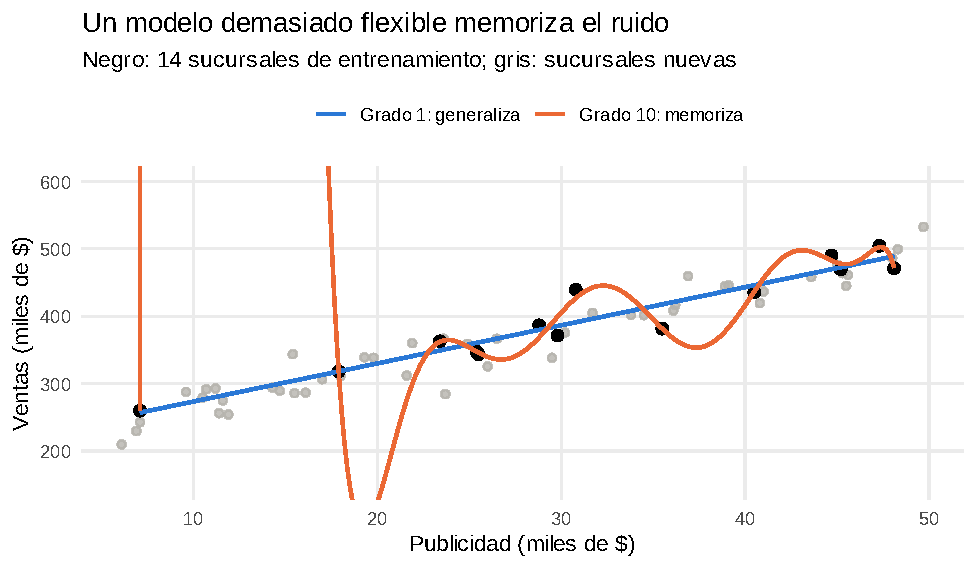
\includegraphics[width=0.9\textwidth]{m07-sobreajuste}
\caption{La recta (azul) captura la relación real; el polinomio de grado 10
(naranja) pasa cerca de cada punto de entrenamiento, pero hace predicciones
absurdas para sucursales nuevas.}
\label{fig:m07-sobreajuste}
\end{figure}

\begin{concepto}{Sesgo y varianza, en una frase}
Un modelo demasiado \textbf{simple} no captura el patrón (\emph{subajuste}); uno
demasiado \textbf{complejo} captura hasta el ruido (\emph{sobreajuste}). El
objetivo es el punto medio, y la única forma honesta de encontrarlo es medir el
error en datos que el modelo no usó para aprender.
\end{concepto}

\subsection{Validación cruzada}
\label{sec:m7-cv}

Con una sola división entrenamiento/prueba, el resultado depende un poco de la
suerte: quizá justo quedaron casos fáciles en la prueba. La
\termino{validación cruzada} de $k$ pliegues (\emph{k-fold cross-validation})
lo resuelve: parte los datos en $k$ grupos (típicamente 5 o 10), entrena $k$
veces dejando fuera un grupo distinto cada vez, y promedia los $k$ errores
(figura~\ref{fig:m7-cv}).

\begin{figure}[H]
\centering
\begin{tikzpicture}[
  bloque/.style={rectangle, draw=white, thick, minimum width=1.9cm,
    minimum height=0.55cm, font=\sffamily\scriptsize},
  ent/.style={bloque, fill=primario!25},
  val/.style={bloque, fill=acento!80, text=white},
]
\foreach \r in {1,...,5} {
  \node[font=\sffamily\small, anchor=east] at (-0.2, -\r*0.7) {Ronda \r};
  \foreach \c in {1,...,5} {
    \ifnum\c=\r
      \node[val] at (\c*1.95, -\r*0.7) {validación};
    \else
      \node[ent] at (\c*1.95, -\r*0.7) {entrena};
    \fi
  }
  \node[font=\sffamily\small, anchor=west] at (10.9, -\r*0.7) {error$_{\r}$};
}
\node[font=\sffamily\small, anchor=west, text=primario] at (10.9, -4.35)
  {\textbf{promedio}};
\end{tikzpicture}
\caption{Validación cruzada de 5 pliegues: cada sucursal se usa 4 veces para
entrenar y exactamente una vez para validar.}
\label{fig:m7-cv}
\end{figure}

Hagámoslo a mano una vez, para entender lo que después hará \paquete{caret}
automáticamente. Comparamos la recta con polinomios de grado 3, 6 y 10 usando
las 60 sucursales:

\begin{rcode}
set.seed(123)
# Asigna cada sucursal a uno de 5 pliegues, al azar y en partes iguales
pliegue <- sample(rep(1:5, length.out = nrow(sucursales)))
table(pliegue)

error_cv <- function(grado) {
  errores <- map_dbl(1:5, function(k) {
    entrena <- sucursales[pliegue != k, ]   # 4 pliegues para aprender
    valida  <- sucursales[pliegue == k, ]   # 1 pliegue para evaluar
    modelo  <- lm(ventas ~ poly(publicidad, grado), data = entrena)
    rmse(valida$ventas, predict(modelo, valida))
  })
  mean(errores)   # promedio de los 5 errores
}

tibble(grado = c(1, 3, 6, 10)) %>%
  mutate(rmse_cv = map_dbl(grado, error_cv))
\end{rcode}

\begin{rsalida}
pliegue
 1  2  3  4  5 
12 12 12 12 12 
# A tibble: 4 x 2
  grado rmse_cv
  <dbl>   <dbl>
1     1    21.5
2     3    22.2
3     6    22.6
4    10    29.0
\end{rsalida}

Primero, \codigo{table(pliegue)} confirma que cada pliegue tiene 12
sucursales. Luego, la recta tiene el menor error de validación cruzada (21.5
mil pesos), y el error crece con la complejidad hasta 29.0 con el grado 10. La
validación cruzada llega a la misma conclusión que la figura, pero usando las
60 sucursales y sin depender de una sola división afortunada. En la práctica
la usarás para \textbf{elegir entre modelos o ajustar sus parámetros}, y
reservarás el conjunto de prueba para la evaluación final.

\subsection{Fuga de datos: el error más caro}
\label{sec:m7-fuga}

La \termino{fuga de datos} (\emph{data leakage}) ocurre cuando, al entrenar, el
modelo tiene acceso a información que \textbf{no estará disponible en el
momento real de predecir}. El resultado es un modelo espectacular en el
laboratorio y inútil en la operación. Es el error más común y más caro del
machine learning, porque no produce ningún mensaje de error: produce
\emph{optimismo}.

\begin{negocio}{Un modelo de abandono ``perfecto''}
Un equipo entrena un modelo de churn y obtiene 98\% de exactitud. Entre las
predictoras incluyó \codigo{dias\_desde\_ultima\_llamada\_a\_cancelaciones}.
Pero los clientes llaman al área de cancelaciones \emph{cuando ya decidieron
irse}: esa variable es una consecuencia del abandono, no una causa observable
con anticipación. En producción, el modelo avisa cuando el cliente ya está
cancelando, demasiado tarde para retenerlo.
\end{negocio}

Formas típicas de fuga en BI:

\begin{itemize}
  \item \textbf{Variables del futuro}: motivo de cancelación, fecha de baja,
        monto de reembolso, ``estatus final'' del pedido.
  \item \textbf{Variables calculadas con la respuesta}: como el
        \codigo{total\_transaccion} que ya contiene a \codigo{cantidad}.
  \item \textbf{Preprocesar con todos los datos}: escalar, imputar o calcular
        promedios usando también los datos de prueba antes de separarlos.
  \item \textbf{Series de tiempo mezcladas}: separar al azar meses de una serie
        (entrenas con marzo de 2025 para ``predecir'' febrero de 2025). En series
        de tiempo, la prueba siempre son los periodos más recientes.
\end{itemize}

En la sección de errores comunes (sección~\ref{sec:m7-errores}) verás con
código cómo una sola variable con fuga convierte un modelo mediocre en uno
aparentemente perfecto.

\begin{hazlotu}
Piensa en tu empresa: escribe tres variables que \emph{parecerían} excelentes
para predecir si un pedido llegará tarde, pero que en realidad solo se conocen
después de la entrega.
\end{hazlotu}

% ============================================================================
\section{Caso 1: segmentación de clientes con RFM y k-means}
\label{sec:m7-segmentacion}

\begin{ejemplo}{¿A quién le mandamos la campaña VIP?}
El área de marketing tiene presupuesto para tres campañas distintas y quiere
dejar de mandar el mismo correo a los 200 clientes. La pregunta es: \emph{¿qué
grupos de clientes con comportamiento de compra parecido tenemos y qué
estrategia conviene para cada uno?} Es un problema \textbf{no supervisado}: no
hay una respuesta correcta que predecir; queremos descubrir grupos. Usaremos
los datos reales del curso: \archivo{transacciones.csv} y
\archivo{clientes.csv}.
\end{ejemplo}

\subsection{Paso 1: calcular Recencia, Frecuencia y Monto}

\begin{concepto}{RFM}
El análisis \termino{RFM} resume el comportamiento de cada cliente en tres
números, muy usados en retail y marketing directo:
\begin{itemize}
  \item \textbf{Recencia (R):} días desde su última compra. \emph{Menos} es
        mejor: quien compró hace poco tiene más probabilidad de volver.
  \item \textbf{Frecuencia (F):} número de compras en el periodo. Más es mejor.
  \item \textbf{Monto (M):} dinero total gastado en el periodo. Más es mejor.
\end{itemize}
La recencia se mide respecto a una \termino{fecha de corte} fija (por ejemplo,
el día en que haces el análisis). Fíjala en el código; si usas
\codigo{Sys.Date()}, tus resultados cambiarán cada día.
\end{concepto}

Las transacciones cubren todo 2023, así que usaremos como fecha de corte el
1 de enero de 2024:

\begin{rcode}
clientes <- read_csv("datasets/clientes.csv", show_col_types = FALSE)

fecha_corte <- as.Date("2024-01-01")   # fecha fija del análisis

rfm <- transacciones %>%
  group_by(cliente_id) %>%
  summarise(
    ultima_compra = max(fecha),
    recencia   = as.numeric(fecha_corte - ultima_compra),  # días
    frecuencia = n(),                                      # compras
    monto      = sum(total_transaccion),                   # pesos
    .groups = "drop"
  )

rfm
\end{rcode}

\begin{rsalida}
# A tibble: 198 x 5
   cliente_id ultima_compra recencia frecuencia  monto
        <dbl> <date>           <dbl>      <int>  <dbl>
 1          1 2023-12-01          31          7  4859.
 2          2 2023-12-02          30          5  7950.
 3          3 2023-11-04          58          8  9562 
 4          4 2023-12-24           8          5  7759.
 5          5 2023-12-31           1         13 14680.
 6          6 2023-12-31           1          6  6087.
 7          7 2023-12-13          19          5  1552.
 8          8 2023-12-05          27          5  3555.
 9          9 2023-12-23           9          6  5071.
10         10 2023-07-09         176          4  2487.
# i 188 more rows
\end{rsalida}

Cada fila es ahora un cliente. El cliente 1, por ejemplo, compró por última vez
el 1 de diciembre (31 días antes del corte), hizo 7 compras y gastó \$4{,}859.
Hay 198 filas, pero \archivo{clientes.csv} tiene 200 clientes. ¿Quiénes faltan?

\begin{rcode}
# Clientes registrados que no aparecen en las transacciones
clientes %>%
  anti_join(rfm, by = "cliente_id") %>%
  select(cliente_id, nombre, fecha_registro)
\end{rcode}

\begin{rsalida}
# A tibble: 2 x 3
  cliente_id nombre            fecha_registro
       <dbl> <chr>             <date>        
1        171 Rosa Jiménez      2022-08-27    
2        199 Ricardo Hernández 2023-09-16    
\end{rsalida}

Dos clientes no compraron nada en 2023. No entran al clustering (no tienen
recencia ni frecuencia), pero no los olvides: en la práctica formarían su propio
grupo, ``registrados sin compra'', con una estrategia de activación.

\begin{rcode}
rfm %>%
  select(recencia, frecuencia, monto) %>%
  summary()
\end{rcode}

\begin{rsalida}
    recencia        frecuencia         monto        
 Min.   :  1.00   Min.   : 1.000   Min.   :  152.6  
 1st Qu.: 21.00   1st Qu.: 3.000   1st Qu.: 3101.4  
 Median : 48.00   Median : 5.000   Median : 4521.8  
 Mean   : 69.19   Mean   : 5.051   Mean   : 4848.4  
 3rd Qu.: 98.75   3rd Qu.: 6.000   3rd Qu.: 6183.0  
 Max.   :314.00   Max.   :13.000   Max.   :14680.1  
\end{rsalida}

Observa las escalas: la recencia va de 1 a 314 días, la frecuencia de 1 a 13
compras y el monto de 153 a 14{,}680 pesos. Esto es crucial para el siguiente
paso.

\subsection{Paso 2: escalar las variables}

\begin{concepto}{Por qué escalar antes de k-means}
\termino{k-means} agrupa clientes según la \emph{distancia} entre ellos. Si una
variable se mide en miles (monto) y otra en unidades (frecuencia), la distancia
la domina casi por completo la de números grandes: una diferencia de 2 compras
``pesaría'' lo mismo que una diferencia de 2 pesos. \termino{Escalar}
(estandarizar) convierte cada variable a media 0 y desviación estándar 1, para
que las tres pesen lo mismo. En R se hace con \codigo{scale()}.
\end{concepto}

\begin{rcode}
rfm_escalado <- rfm %>%
  select(recencia, frecuencia, monto) %>%
  scale()                     # (x - media) / desviación estándar

round(colMeans(rfm_escalado), 2)          # medias: todas 0
round(apply(rfm_escalado, 2, sd), 2)      # desviaciones: todas 1
head(round(rfm_escalado, 2), 3)
\end{rcode}

\begin{rsalida}
  recencia frecuencia      monto 
         0          0          0 
  recencia frecuencia      monto 
         1          1          1 
     recencia frecuencia monto
[1,]    -0.59       0.85  0.00
[2,]    -0.60      -0.02  1.15
[3,]    -0.17       1.28  1.75
\end{rsalida}

Un valor escalado se lee como ``cuántas desviaciones estándar está este cliente
por arriba o por debajo del promedio''. El primer cliente tiene una recencia de
$-0.59$: compró más recientemente que el cliente promedio. \codigo{scale()}
guarda las medias y desviaciones usadas como atributos del resultado; los
necesitaremos después para asignar clientes nuevos.

\subsection{Paso 3: ¿cuántos grupos? Método del codo y silueta}

k-means necesita que le digas cuántos grupos ($k$) formar. Dos herramientas
ayudan a decidir:

\begin{itemize}
  \item \textbf{Método del codo:} para cada $k$ calcula la
        \termino{suma de cuadrados dentro de los grupos} (WSS, qué tan
        dispersos están los clientes respecto al centro de su grupo). Siempre
        baja al aumentar $k$; buscamos el ``codo'', el punto a partir del cual
        agregar grupos ya casi no mejora.
  \item \textbf{Silueta:} mide, para cada cliente, qué tan cerca está de su
        propio grupo comparado con el grupo vecino (de $-1$ a $1$; más alto es
        mejor). Buscamos el $k$ con la silueta promedio más alta.
\end{itemize}

\begin{rcode}
set.seed(123)
codo <- tibble(k = 1:10) %>%
  mutate(wss = map_dbl(k, function(k) {
    kmeans(rfm_escalado, centers = k, nstart = 25)$tot.withinss
  }))

codo %>%
  mutate(mejora_pct = round(100 * (lag(wss) - wss) / lag(wss), 1),
         wss = round(wss, 1))
\end{rcode}

\begin{rsalida}
# A tibble: 10 x 3
       k   wss mejora_pct
   <int> <dbl>      <dbl>
 1     1 591         NA  
 2     2 344.        41.9
 3     3 239         30.5
 4     4 175.        26.9
 5     5 146.        16.3
 6     6 127.        13  
 7     7 114         10.5
 8     8 102.        10.3
 9     9  92.3        9.7
10    10  85.1        7.8
\end{rsalida}

La columna \codigo{mejora\_pct} dice cuánto baja la dispersión al agregar un
grupo más. Pasar de 1 a 2 grupos reduce la WSS 41.9\%; de 2 a 3, 30.5\%; de 3 a
4, 26.9\%; y a partir de ahí las mejoras son cada vez menores. Veámoslo en una
gráfica, resaltando $k = 4$:

\begin{rcode}
grafico_codo <- ggplot(codo, aes(x = k, y = wss)) +
  geom_line(color = color_principal, linewidth = 0.8) +
  geom_point(color = color_principal, size = 2) +
  geom_point(data = filter(codo, k == 4), color = color_resalte,
             size = 4) +
  annotate("text", x = 4.3, y = codo$wss[4] + 60, hjust = 0,
           label = "k = 4: las mejoras\nempiezan a ser pequeñas",
           color = color_resalte, size = 3.5) +
  scale_x_continuous(breaks = 1:10) +
  labs(title = "Método del codo",
       subtitle = "Dispersión dentro de los grupos según k",
       x = "Número de grupos (k)",
       y = "Suma de cuadrados dentro (WSS)") +
  theme_minimal() +
  theme(panel.grid.minor = element_blank())
grafico_codo
\end{rcode}

\begin{figure}[H]
\centering
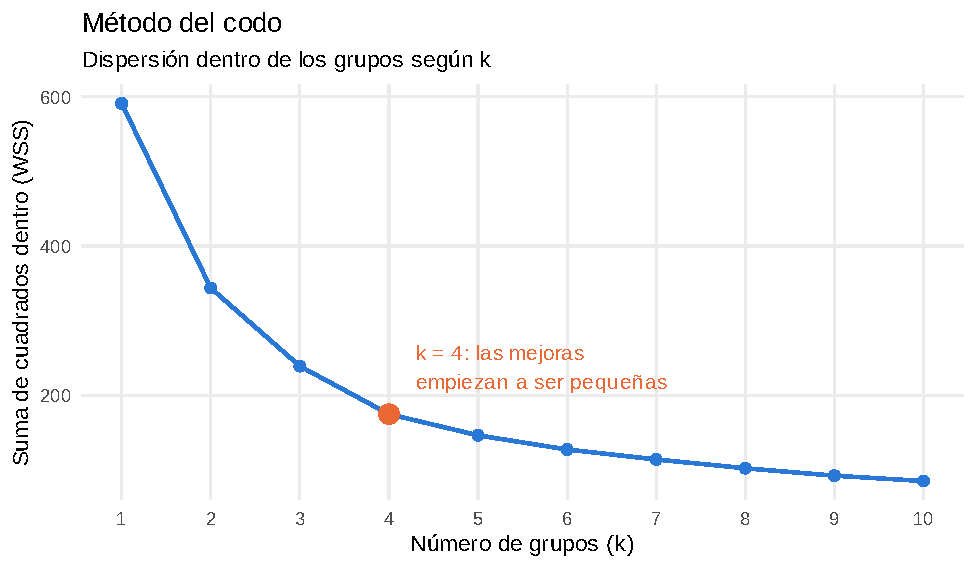
\includegraphics[width=0.9\textwidth]{m07-codo}
\caption{Método del codo para el RFM de los clientes del curso. La curva se
suaviza entre $k = 3$ y $k = 4$.}
\label{fig:m07-codo}
\end{figure}

Ahora la silueta. La función \codigo{fviz\_nbclust()} de \paquete{factoextra}
hace todo el cálculo y devuelve una gráfica de \paquete{ggplot2}, que puedes
personalizar con \codigo{labs()} y \codigo{theme()} como cualquier otra:

\begin{rcode}
set.seed(123)
grafico_silueta <- fviz_nbclust(rfm_escalado, kmeans,
                                method = "silhouette", k.max = 10,
                                nstart = 25, linecolor = color_principal) +
  labs(title = "Silueta promedio según el número de grupos",
       subtitle = "Más alto = grupos más separados",
       x = "Número de grupos (k)", y = "Silueta promedio") +
  theme_minimal() +
  theme(panel.grid.minor = element_blank())
grafico_silueta

# Los valores calculados vienen dentro del objeto ggplot
grafico_silueta$data %>%
  mutate(y = round(y, 3)) %>%
  filter(clusters %in% 2:6)
\end{rcode}

\begin{rsalida}
  clusters     y
1        2 0.345
2        3 0.337
3        4 0.328
4        5 0.325
5        6 0.292
\end{rsalida}

\begin{figure}[H]
\centering
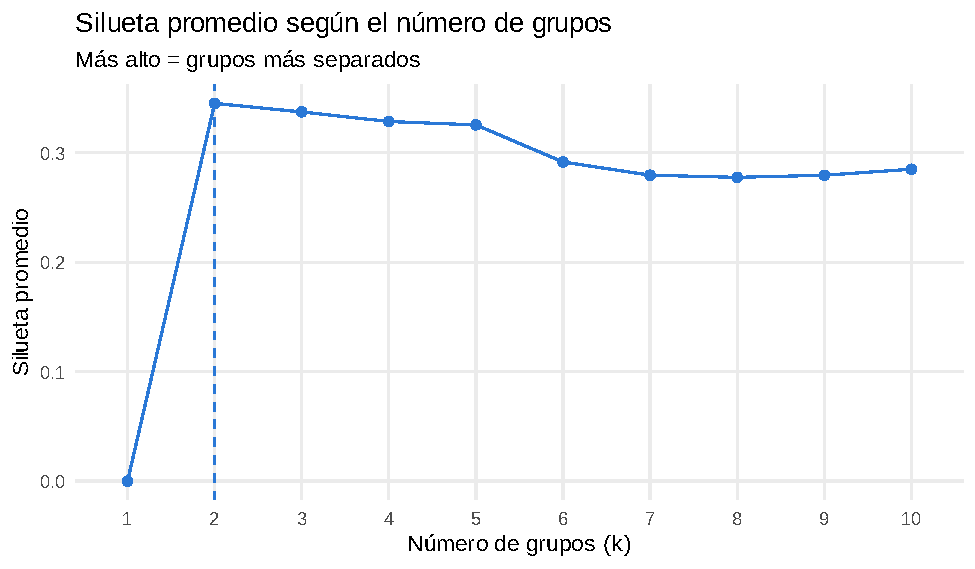
\includegraphics[width=0.9\textwidth]{m07-silueta}
\caption{Silueta promedio para $k$ de 1 a 10. La línea punteada marca el
máximo ($k = 2$), aunque las diferencias entre 2 y 5 grupos son mínimas.}
\label{fig:m07-silueta}
\end{figure}

La silueta más alta es para $k = 2$ (0.345), pero $k = 3$, 4 y 5 están
prácticamente empatados (0.337, 0.328 y 0.325). Una silueta de alrededor de
0.33 indica una estructura \emph{débil}: los clientes no forman ``islas''
naturales, sino un continuo que k-means parte en regiones. Es lo esperable con
datos generados al azar, y muy común con clientes reales.

\begin{consejo}
Cuando las métricas no dan un ganador claro, decide con criterio de negocio.
Dos grupos (``buenos'' y ``malos'') no alcanzan para diseñar tres campañas;
diez grupos son imposibles de operar. Aquí elegimos $k = 4$: el codo lo
respalda, la silueta casi no empeora y el área de marketing puede manejar
cuatro estrategias. Las métricas orientan; la decisión es tuya.
\end{consejo}

\subsection{Paso 4: entrenar k-means}

\begin{concepto}{Cómo trabaja k-means}
\begin{enumerate}
  \item Coloca $k$ centros al azar.
  \item Asigna cada cliente al centro más cercano.
  \item Mueve cada centro al promedio de sus clientes.
  \item Repite 2 y 3 hasta que los grupos ya no cambian.
\end{enumerate}
Como el resultado depende de los centros iniciales, el argumento
\codigo{nstart = 25} prueba 25 arranques distintos y se queda con el mejor
(el de menor WSS). Usa siempre \codigo{set.seed()} y un \codigo{nstart} de 10
o más.
\end{concepto}

\begin{rcode}
set.seed(123)
modelo_kmeans <- kmeans(rfm_escalado, centers = 4, nstart = 25)

modelo_kmeans$size                     # clientes por grupo
round(modelo_kmeans$centers, 2)        # centros (en escala estandarizada)

# Proporción de la variación total explicada por los grupos
round(modelo_kmeans$betweenss / modelo_kmeans$totss, 3)
\end{rcode}

\begin{rsalida}
[1] 22 87 60 29
  recencia frecuencia monto
1    -0.53       1.81  1.97
2    -0.42       0.36  0.27
3    -0.13      -0.71 -0.73
4     1.95      -0.98 -0.80
[1] 0.704
\end{rsalida}

Los centros están en escala estandarizada, así que se leen como ``desviaciones
respecto al promedio''. El grupo 1 tiene frecuencia $+1.81$ y monto $+1.97$:
compra mucho más que el promedio. El grupo 4 tiene recencia $+1.95$: hace mucho
que no compra. Los cuatro grupos explican el 70.4\% de la variación total de los
datos.

\begin{advertencia}
Los números de grupo (1, 2, 3, 4) son etiquetas \textbf{arbitrarias}: si
cambias la semilla, el orden de los datos o la versión de R, el grupo de
``mejores clientes'' puede aparecer como 3 en lugar de 1. Nunca escribas en tu
código \codigo{cluster == 1 \textasciitilde{} "VIP"}. Nombra los grupos a partir
de su perfil calculado, como haremos enseguida.
\end{advertencia}

Revisemos también la calidad de cada grupo con la silueta individual:

\begin{rcode}
silueta <- silhouette(modelo_kmeans$cluster, dist(rfm_escalado))

# Silueta promedio por grupo y cuántos clientes quedaron "mal ubicados"
round(summary(silueta)$clus.avg.widths, 3)
sum(silueta[, "sil_width"] < 0)
\end{rcode}

\begin{rsalida}
    1     2     3     4 
0.375 0.321 0.298 0.379 
[1] 0
\end{rsalida}

Todos los grupos tienen silueta positiva; los más compactos son el 4 (0.379)
y el 1 (0.375), y el menos definido es el 3 (0.298). Ningún cliente tiene
silueta negativa (el \codigo{0} de la última línea): nadie quedó más cerca del
grupo vecino que del suyo. Si hubiera clientes con silueta negativa, serían
clientes ``frontera'' que conviene revisar a mano.

\subsection{Paso 5: perfilar y nombrar los segmentos}

Un segmento no sirve hasta que alguien de negocio puede describirlo en una
frase. Calculamos el perfil de cada grupo \emph{en las unidades originales}
(días, compras, pesos) y su peso en clientes e ingresos:

\begin{rcode}
rfm_seg <- rfm %>%
  mutate(cluster = modelo_kmeans$cluster)

perfil <- rfm_seg %>%
  group_by(cluster) %>%
  summarise(
    clientes        = n(),
    recencia_prom   = mean(recencia),
    frecuencia_prom = mean(frecuencia),
    monto_prom      = mean(monto),
    ingresos        = sum(monto),
    .groups = "drop"
  ) %>%
  mutate(pct_clientes = 100 * clientes / sum(clientes),
         pct_ingresos = 100 * ingresos / sum(ingresos))

perfil %>%
  select(cluster, clientes, recencia_prom, frecuencia_prom, monto_prom,
         pct_ingresos) %>%
  mutate(across(where(is.double), ~ round(.x, 1)))
\end{rcode}

\begin{rsalida}
# A tibble: 4 x 6
  cluster clientes recencia_prom frecuencia_prom monto_prom
    <int>    <int>         <dbl>           <dbl>      <dbl>
1       1       22          34.5             9.2     10159.
2       2       87          41.8             5.9      5577.
3       3       60          60.5             3.4      2879.
4       4       29         196.              2.8      2708.
# i 1 more variable: pct_ingresos <dbl>
\end{rsalida}

Ahora asignamos los nombres \textbf{con una regla basada en el perfil}, no en
el número del grupo. La regla de negocio es: el grupo con la recencia promedio
más alta son los ``Dormidos''; los demás se ordenan por monto promedio de mayor
a menor y se llaman ``Campeones'', ``Leales'' y ``Ocasionales''.

\begin{rcode}
nombres_segmentos <- perfil %>%
  mutate(es_dormido = recencia_prom == max(recencia_prom)) %>%
  arrange(es_dormido, desc(monto_prom)) %>%   # dormidos al final
  mutate(segmento = c("Campeones", "Leales", "Ocasionales",
                      "Dormidos")) %>%
  select(cluster, segmento)

orden_segmentos <- c("Campeones", "Leales", "Ocasionales", "Dormidos")

rfm_seg <- rfm_seg %>%
  left_join(nombres_segmentos, by = "cluster") %>%
  mutate(segmento = factor(segmento, levels = orden_segmentos))

perfil_segmentos <- perfil %>%
  left_join(nombres_segmentos, by = "cluster") %>%
  mutate(segmento = factor(segmento, levels = orden_segmentos)) %>%
  arrange(segmento) %>%
  transmute(segmento, clientes,
            recencia_dias = round(recencia_prom),
            compras       = round(frecuencia_prom, 1),
            monto_prom    = round(monto_prom),
            pct_ingresos  = round(pct_ingresos, 1))
perfil_segmentos
\end{rcode}

\begin{rsalida}
# A tibble: 4 x 6
  segmento    clientes recencia_dias compras monto_prom pct_ingresos
  <fct>          <int>         <dbl>   <dbl>      <dbl>        <dbl>
1 Campeones         22            35     9.2      10159         23.3
2 Leales            87            42     5.9       5577         50.5
3 Ocasionales       60            60     3.4       2879         18  
4 Dormidos          29           195     2.8       2708          8.2
\end{rsalida}

Ahora sí, cada grupo cuenta una historia:

\begin{itemize}
  \item \textbf{Campeones} (22 clientes, 11\% de la base): compraron hace unos
        35 días, 9.2 veces en el año y gastaron en promedio \$10{,}159. Son
        apenas uno de cada nueve clientes, pero generan el 23.3\% de los
        ingresos.
  \item \textbf{Leales} (87 clientes): el grueso de la base. Compran seguido
        (5.9 veces) y aportan la mitad de los ingresos (50.5\%).
  \item \textbf{Ocasionales} (60): activos (60 días de recencia), pero compran
        poco y gastan \$2{,}879 en promedio.
  \item \textbf{Dormidos} (29): su última compra fue hace 195 días en
        promedio, más de seis meses. Aportan solo 8.2\% de los ingresos.
\end{itemize}

Observa que la regla de nombres no menciona ningún número de grupo: si mañana
k-means numera distinto, cada cliente seguirá recibiendo el nombre correcto.

\begin{hazlotu}
Cambia la semilla a \codigo{set.seed(2024)} antes de \codigo{kmeans()} y vuelve
a correr los pasos 4 y 5. ¿Cambian los números de grupo? ¿Cambian los nombres
asignados a cada cliente? (Deberían mantenerse, porque los nombres dependen del
perfil y no del número.)
\end{hazlotu}

\subsection{Paso 6: visualizar los segmentos}

\codigo{fviz\_cluster()} dibuja los grupos en dos dimensiones. Como tenemos tres
variables, primero las resume en dos ``componentes principales'' (combinaciones
de R, F y M que conservan la mayor parte de la información); los porcentajes de
los ejes indican cuánta información conserva cada una.

\begin{rcode}
grafico_clusters <- fviz_cluster(modelo_kmeans, data = rfm_escalado,
                                 geom = "point", ellipse.type = "convex",
                                 palette = paleta_libro[1:4],
                                 ggtheme = theme_minimal()) +
  labs(title = "Grupos de k-means sobre el RFM escalado",
       subtitle = "Proyección en los dos componentes principales",
       color = "Grupo", fill = "Grupo", shape = "Grupo")
grafico_clusters
\end{rcode}

\begin{figure}[H]
\centering
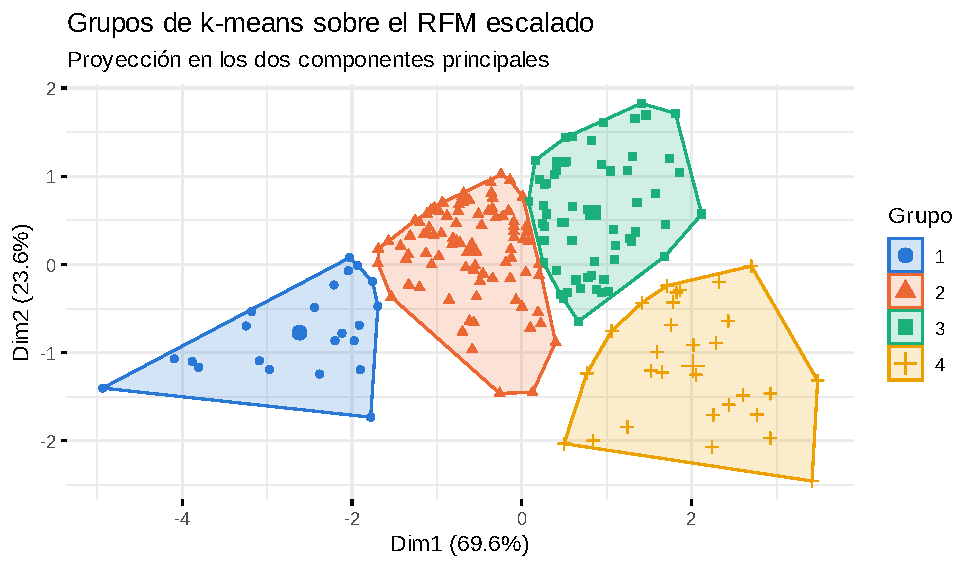
\includegraphics[width=0.9\textwidth]{m07-clusters}
\caption{Los cuatro grupos de k-means proyectados en dos componentes
principales, que juntos conservan 93.2\% de la información de R, F y M.}
\label{fig:m07-clusters}
\end{figure}

La gráfica de componentes principales es útil para ver si los grupos se
separan, pero sus ejes son difíciles de explicar a la dirección. Para una
presentación, grafica las variables originales con los nombres de negocio:

\begin{rcode}
grafico_segmentos <- ggplot(rfm_seg,
                            aes(recencia, monto, color = segmento)) +
  geom_point(size = 2, alpha = 0.8) +
  scale_color_manual(values = paleta_libro[1:4]) +
  scale_y_continuous(labels = scales::dollar) +
  labs(title = "Segmentos de clientes según recencia y monto",
       subtitle = "Clientes del curso, compras de 2023",
       x = "Días desde la última compra (recencia)",
       y = "Monto total comprado", color = NULL) +
  theme_minimal() +
  theme(panel.grid.minor = element_blank(), legend.position = "top")
grafico_segmentos
\end{rcode}

\begin{figure}[H]
\centering
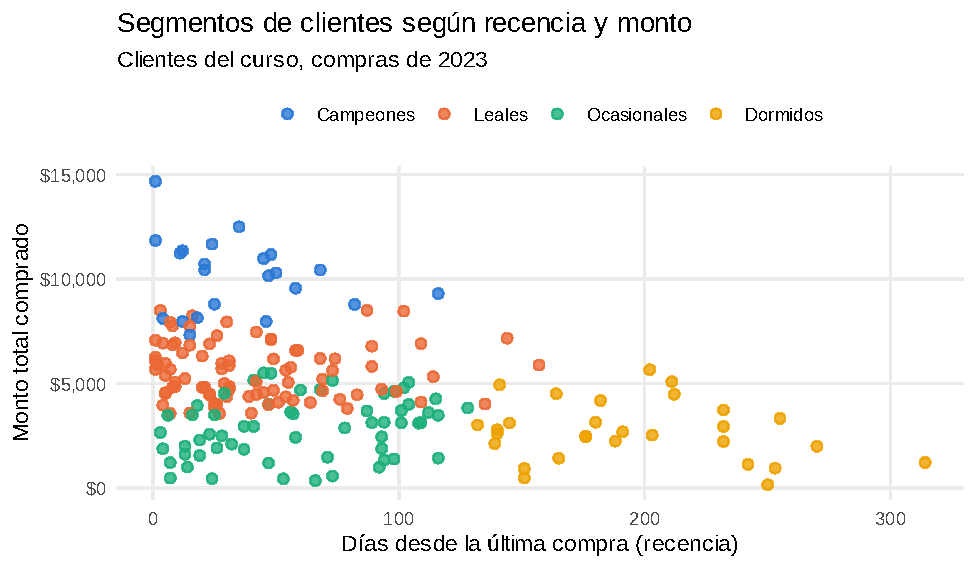
\includegraphics[width=0.9\textwidth]{m07-segmentos}
\caption{Segmentos RFM en unidades de negocio: los Dormidos se separan por
recencia; Campeones, Leales y Ocasionales, por monto.}
\label{fig:m07-segmentos}
\end{figure}

\subsection{Paso 7: de segmentos a estrategias}

La segmentación solo genera valor cuando cada segmento tiene una acción
asociada. La tabla~\ref{tab:m7-estrategias} es un ejemplo de cómo se
presentaría a marketing.

\begin{table}[H]
\centering
\small
\caption{Estrategia sugerida por segmento RFM.}
\label{tab:m7-estrategias}
\begin{tabularx}{\textwidth}{>{\raggedright\arraybackslash}p{2.2cm}
                              >{\raggedright\arraybackslash}p{4.2cm}
                              >{\raggedright\arraybackslash}X}
\toprule
\textbf{Segmento} & \textbf{Quiénes son} & \textbf{Estrategia} \\
\midrule
Campeones & Compran seguido, gastan el doble del promedio y compraron hace poco. &
  Programa VIP, acceso anticipado a lanzamientos, atención preferente. No
  regalar descuentos: ya compran sin ellos. \\
Leales & Compradores regulares con gasto por encima del promedio. &
  Venta cruzada y \emph{up-selling} (sección~\ref{sec:m7-canasta}); programa
  de puntos para convertirlos en Campeones. \\
Ocasionales & Compran poco y gastan poco, pero siguen activos. &
  Campañas de frecuencia: cupones con fecha de vencimiento, recordatorios,
  paquetes de entrada. \\
Dormidos & No compran desde hace más de seis meses en promedio. &
  Campaña de reactivación con oferta fuerte y encuesta de salida; si no
  responden, reducir la inversión en ellos. \\
\bottomrule
\end{tabularx}
\end{table}

Para enriquecer el perfil, puedes unir los segmentos con los datos
demográficos de \archivo{clientes.csv}. Por ejemplo, ¿los Campeones son más
``premium'' o más jóvenes?

\begin{rcode}
rfm_seg %>%
  # de clientes.csv solo tomamos lo que necesitamos (ya trae una
  # columna "segmento" por edad que chocaría con la nuestra)
  left_join(select(clientes, cliente_id, edad, es_premium),
            by = "cliente_id") %>%
  group_by(segmento) %>%
  summarise(clientes    = n(),
            edad_prom   = round(mean(edad), 1),
            pct_premium = round(100 * mean(es_premium), 1),
            .groups = "drop")
\end{rcode}

\begin{rsalida}
# A tibble: 4 x 4
  segmento    clientes edad_prom pct_premium
  <fct>          <int>     <dbl>       <dbl>
1 Campeones         22      49.2        31.8
2 Leales            87      47.4        34.5
3 Ocasionales       60      49.2        45  
4 Dormidos          29      51.3        27.6
\end{rsalida}

La edad promedio es casi igual en los cuatro segmentos (47 a 51 años) y el
porcentaje de clientes \emph{premium} no sigue ningún patrón lógico: los
Ocasionales tienen más premium (45\%) que los Campeones (31.8\%). En estos datos
simulados, la membresía premium y la edad no tienen relación con el
comportamiento de compra. En una empresa real este cruce sería un hallazgo
importante: si pagas beneficios premium a clientes que compran poco, el
programa necesita revisión.

\subsection{Paso 8: asignar un segmento a clientes nuevos}

El modelo ya está entrenado. Cuando un cliente acumula historial, no necesitas
volver a correr k-means: basta con escalar sus valores \textbf{con las mismas
medias y desviaciones del entrenamiento} y asignarlo al centro más cercano.

\begin{rcode}
asignar_segmento <- function(nuevos, modelo, datos_escalados, nombres) {
  medias   <- attr(datos_escalados, "scaled:center")
  desv_est <- attr(datos_escalados, "scaled:scale")
  # Escalamos con los parámetros del entrenamiento (no con los nuevos)
  nuevos_esc <- scale(nuevos[, names(medias)], center = medias,
                      scale = desv_est)
  # Para cada cliente: el centro con menor distancia al cuadrado
  grupo <- apply(nuevos_esc, 1, function(fila) {
    which.min(colSums((t(modelo$centers) - fila)^2))
  })
  nuevos %>%
    mutate(cluster = grupo) %>%
    left_join(nombres, by = "cluster")
}

nuevos_clientes <- tibble(
  cliente    = c("Ana", "Beto", "Carla"),
  recencia   = c(10, 250, 45),
  frecuencia = c(11, 2, 4),
  monto      = c(9500, 1800, 3500)
)

asignar_segmento(nuevos_clientes, modelo_kmeans, rfm_escalado,
                 nombres_segmentos)
\end{rcode}

\begin{rsalida}
# A tibble: 3 x 6
  cliente recencia frecuencia monto cluster segmento   
  <chr>      <dbl>      <dbl> <dbl>   <int> <chr>      
1 Ana           10         11  9500       1 Campeones  
2 Beto         250          2  1800       4 Dormidos   
3 Carla         45          4  3500       3 Ocasionales
\end{rsalida}

Ana (compró hace 10 días, 11 compras, \$9{,}500) es Campeona; Beto, que no
compra desde hace 250 días, cae en Dormidos; y Carla, con un comportamiento
modesto pero reciente, en Ocasionales. Este tipo de función es la que después
se programa para que corra cada semana (Módulo~\ref{cap:reportes}).

\subsection{Alternativa sencilla: RFM por reglas con quintiles}

No siempre necesitas k-means. Muchas empresas usan \termino{RFM por reglas}: a
cada cliente se le asigna una calificación de 1 a 5 en cada dimensión según su
quintil (el 20\% con mejor valor recibe 5) y luego se definen segmentos con
reglas fáciles de explicar. En R, \codigo{ntile()} de \paquete{dplyr} hace el
trabajo.

\begin{rcode}
rfm_reglas <- rfm %>%
  mutate(
    r_score = ntile(desc(recencia), 5),   # 5 = compró más recientemente
    f_score = ntile(frecuencia, 5),       # 5 = compra más seguido
    m_score = ntile(monto, 5),            # 5 = gasta más
    codigo_rfm = paste0(r_score, f_score, m_score),
    segmento_reglas = case_when(
      r_score >= 4 & f_score >= 4 & m_score >= 4 ~ "Campeones",
      r_score >= 3 & f_score >= 3                ~ "Leales",
      r_score <= 2 & f_score >= 3                ~ "En riesgo",
      r_score <= 2                               ~ "Dormidos",
      TRUE                                       ~ "Ocasionales"
    )
  )

rfm_reglas %>%
  select(cliente_id, recencia, frecuencia, monto, codigo_rfm,
         segmento_reglas) %>%
  head(5)

rfm_reglas %>% count(segmento_reglas, sort = TRUE)
\end{rcode}

\begin{rsalida}
# A tibble: 5 x 6
  cliente_id recencia frecuencia  monto codigo_rfm segmento_reglas
       <dbl>    <dbl>      <int>  <dbl> <chr>      <chr>          
1          1       31          7  4859. 443        Leales         
2          2       30          5  7950. 435        Leales         
3          3       58          8  9562  355        Leales         
4          4        8          5  7759. 535        Leales         
5          5        1         13 14680. 555        Campeones      
# A tibble: 5 x 2
  segmento_reglas     n
  <chr>           <int>
1 Leales             56
2 Dormidos           50
3 Campeones          32
4 En riesgo          30
5 Ocasionales        30
\end{rsalida}

El cliente 1 tiene código 443 (recencia y frecuencia altas, monto medio): no
alcanza el 4 en monto para ser Campeón y cae en ``Leales''. Ahora un segmento nuevo aparece: ``En riesgo'', clientes que
\emph{solían} comprar seguido pero llevan tiempo sin volver; k-means los había
repartido entre otros grupos. ¿Qué tanto coinciden ambos métodos?

\begin{rcode}
table(Reglas = rfm_reglas$segmento_reglas, kmeans = rfm_seg$segmento)
\end{rcode}

\begin{rsalida}
             kmeans
Reglas        Campeones Leales Ocasionales Dormidos
  Campeones          12     20           0        0
  Dormidos            0      1          23       26
  En riesgo           3     19           5        3
  Leales              7     44           5        0
  Ocasionales         0      3          27        0
\end{rsalida}

Las filas son los segmentos por reglas y las columnas los de k-means. La
coincidencia es buena en los extremos: 27 de los 30 Ocasionales por reglas son
Ocasionales en k-means y 26 de los 29 Dormidos de k-means son Dormidos por
reglas. Los 30 clientes ``En riesgo'' se reparten entre Leales (19) y otros
grupos: k-means los mezcló con clientes activos porque su monto y frecuencia
pesan más que su recencia. Ningún método es ``el correcto''; son dos formas de
mirar a los mismos clientes.

\begin{negocio}{¿Reglas o k-means?}
Las reglas RFM son transparentes (``Campeón = calificación 4 o 5 en todo''),
estables en el tiempo y fáciles de programar incluso en SQL o Excel. k-means
descubre grupos sin que tú fijes los cortes y admite más variables (margen,
categorías compradas, devoluciones), pero sus grupos pueden moverse al
reentrenar. Muchas empresas empiezan con reglas y pasan a clustering cuando
necesitan más variables.
\end{negocio}

\begin{hazlotu}
Agrega al RFM una cuarta variable: el número de tiendas distintas en las que
compró cada cliente (\codigo{n\_distinct(tienda\_id)}). Escala, vuelve a correr
k-means con $k = 4$ y compara los perfiles. ¿Aparece algún grupo nuevo con
sentido de negocio?
\end{hazlotu}

% ============================================================================
\section{Caso 2: regresión para predecir ventas}
\label{sec:m7-regresion}

\begin{ejemplo}{¿Cuánto venderá una tienda nueva?}
Una cadena con 400 tiendas planea abrir sucursales y quiere estimar sus ventas
mensuales antes de firmar el contrato de renta. Para cada tienda existente
conoce su zona, tamaño en m², tráfico peatonal mensual, inversión en
publicidad local y si participa en el programa de promociones. La pregunta:
\emph{¿cuánto venderá una tienda con ciertas características y qué palancas
mueven más las ventas?} Es un problema de \textbf{regresión}: la respuesta es
un número.
\end{ejemplo}

\subsection{Datos simulados con una relación conocida}

Como explicamos al inicio, los datos del curso no tienen esta información
(\archivo{tiendas.csv} solo tiene 10 tiendas y sin publicidad), así que
simulamos 400 tiendas. Las ventas mensuales (en miles de pesos) se generan con
esta ``verdad'' que el modelo tendrá que descubrir:

\[
\text{ventas} = 120 + 3.2\,\text{publicidad} + 0.25\,\text{m}^2 +
0.04\,\text{tráfico} + 60\,\text{promoción} + \text{efecto zona} + \text{ruido}
\]

con efecto zona de $+40$ en el Norte, $-30$ en el Sur y 0 en el Centro. El
tráfico depende en parte del tamaño (las tiendas grandes atraen más gente),
como en la vida real.

\begin{rcode}
set.seed(123)
n_tiendas <- 400
tiendas_sim <- tibble(
  tienda     = sprintf("T%03d", 1:n_tiendas),
  zona       = sample(c("Centro", "Norte", "Sur"), n_tiendas,
                      replace = TRUE),
  tamano_m2  = round(runif(n_tiendas, 150, 1200)),
  publicidad = round(runif(n_tiendas, 10, 120), 1),  # miles de $/mes
  promocion  = rbinom(n_tiendas, 1, 0.35),           # 1 = participa
  trafico    = round(3000 + 5 * tamano_m2 +          # personas/mes
                       rnorm(n_tiendas, 0, 1500))
) %>%
  mutate(
    efecto_zona = case_when(zona == "Norte" ~ 40,
                            zona == "Sur"   ~ -30,
                            TRUE            ~ 0),
    ventas = round(120 + 3.2 * publicidad + 0.25 * tamano_m2 +
                     0.04 * trafico + 60 * promocion + efecto_zona +
                     rnorm(n_tiendas, 0, 50), 1)       # miles de $/mes
  ) %>%
  select(-efecto_zona)   # el modelo no debe ver la "respuesta secreta"

head(tiendas_sim, 4)
\end{rcode}

\begin{rsalida}
# A tibble: 4 x 7
  tienda zona  tamano_m2 publicidad promocion trafico ventas
  <chr>  <chr>     <dbl>      <dbl>     <int>   <dbl>  <dbl>
1 T001   Sur         508       17.9         0    5980   517.
2 T002   Sur         638       10.4         0    3903   408.
3 T003   Sur         237       15.7         0    5900   400.
4 T004   Norte      1053      105.          1   10671  1263.
\end{rsalida}

Separamos 80\% para entrenar y 20\% para probar:

\begin{rcode}
set.seed(123)
filas_ent <- sample(nrow(tiendas_sim), size = 0.8 * nrow(tiendas_sim))
tiendas_ent    <- tiendas_sim[filas_ent, ]    # 320 tiendas
tiendas_prueba <- tiendas_sim[-filas_ent, ]   # 80 tiendas
c(entrenamiento = nrow(tiendas_ent), prueba = nrow(tiendas_prueba))
\end{rcode}

\begin{rsalida}
entrenamiento        prueba 
          320            80 
\end{rsalida}

\subsection{Regresión lineal múltiple}

La \termino{regresión lineal múltiple} (función \codigo{lm()}, que ya usaste en
el Módulo~\ref{cap:eda} con una sola variable) estima cuánto cambia la
respuesta por cada unidad de cada predictora, \emph{manteniendo las demás
constantes}. La fórmula \codigo{ventas \textasciitilde{} publicidad + tamano\_m2 + \ldots}
se lee ``ventas en función de publicidad, tamaño, \ldots''.

\begin{rcode}
modelo_lm <- lm(ventas ~ publicidad + tamano_m2 + trafico + promocion +
                  zona, data = tiendas_ent)
summary(modelo_lm)
\end{rcode}

\begin{rsalida}

Call:
lm(formula = ventas ~ publicidad + tamano_m2 + trafico + promocion + 
    zona, data = tiendas_ent)

Residuals:
     Min       1Q   Median       3Q      Max 
-120.181  -38.036   -1.857   35.175  141.550 

Coefficients:
              Estimate Std. Error t value Pr(>|t|)    
(Intercept) 107.296043  11.071131   9.692  < 2e-16 ***
publicidad    3.259854   0.091005  35.821  < 2e-16 ***
tamano_m2     0.270330   0.013935  19.399  < 2e-16 ***
trafico       0.038681   0.001903  20.330  < 2e-16 ***
promocion    57.226212   6.042430   9.471  < 2e-16 ***
zonaNorte    41.704523   6.880492   6.061 3.88e-09 ***
zonaSur     -29.067746   6.992714  -4.157 4.17e-05 ***
---
Signif. codes:  0 '***' 0.001 '**' 0.01 '*' 0.05 '.' 0.1 ' ' 1

Residual standard error: 50.65 on 313 degrees of freedom
Multiple R-squared:  0.937,	Adjusted R-squared:  0.9358 
F-statistic:   776 on 6 and 313 DF,  p-value: < 2.2e-16
\end{rsalida}

\begin{concepto}{Cómo leer la tabla de coeficientes}
\begin{itemize}
  \item \textbf{Estimate}: el efecto estimado. Para una variable numérica, es
        el cambio en ventas por cada unidad adicional; para una categoría
        (\codigo{zonaNorte}), es la diferencia respecto a la categoría base
        (Centro, la primera en orden alfabético).
  \item \textbf{Pr(>|t|)} (valor p): si es muy pequeño (menor a 0.05), el
        efecto difícilmente se debe al azar. Los asteriscos lo resumen.
  \item \textbf{Residual standard error}: el tamaño típico del error del
        modelo, en unidades de la respuesta.
  \item \textbf{R-squared}: proporción de la variación de las ventas que el
        modelo explica.
\end{itemize}
\end{concepto}

Traducido al lenguaje de negocio (recuerda que ventas y publicidad están en
miles de pesos):

\begin{itemize}
  \item \textbf{Publicidad:} cada \$1{,}000 adicionales de publicidad se asocian
        con \$3{,}260 más de ventas mensuales. El valor real era 3.2: el modelo
        lo descubrió.
  \item \textbf{Tamaño:} cada m² adicional aporta unos \$270 al mes (real: 250).
  \item \textbf{Tráfico:} cada 100 visitantes más, \$3{,}900 más de ventas
        (0.039 $\times$ 100, real: 0.04).
  \item \textbf{Promoción:} participar suma unos \$57{,}000 al mes (real: 60).
  \item \textbf{Zona:} una tienda del Norte vende \$41{,}700 más que una
        equivalente del Centro; una del Sur, \$29{,}100 menos.
  \item El modelo explica el 93.7\% de la variación de las ventas
        (R² = 0.937), y el error típico es de unos \$50{,}000, justo el tamaño
        del ruido que simulamos.
\end{itemize}

\begin{advertencia}
Un coeficiente de regresión mide \textbf{asociación, no causalidad}. En datos
simulados sabemos que la publicidad \emph{causa} ventas, porque así lo
programamos. En datos reales, quizá las tiendas que ya venden mucho reciben más
presupuesto de publicidad (la causalidad va al revés). Para afirmar ``si
invierto \$1{,}000 más en publicidad venderé \$3{,}260 más'' necesitas un
experimento (por ejemplo, aumentar la publicidad en tiendas elegidas al azar).
\end{advertencia}

\begin{consejo}
Para saber qué variable ``pesa'' más, no compares los coeficientes
directamente: están en unidades distintas (pesos, m², personas). Compara el
efecto de un cambio \emph{realista}: pasar de 40 a 80 mil pesos de publicidad
suma $40 \times 3.26 \approx 130$ mil pesos; pasar de 400 a 800 m² suma
$400 \times 0.27 \approx 108$ mil pesos directamente, más el tráfico extra que
atrae.
\end{consejo}

\subsection{Evaluar el modelo: MAE, RMSE, MAPE y R²}
\label{sec:m7-metricas-reg}

El resumen del modelo describe el ajuste en los datos de entrenamiento. La
evaluación honesta se hace con las 80 tiendas de prueba. Las cuatro métricas
de regresión más usadas son:

\begin{table}[H]
\centering
\small
\caption{Métricas de error para regresión.}
\label{tab:m7-metricas-reg}
\begin{tabularx}{\textwidth}{>{\raggedright\arraybackslash}p{2.2cm}
                              >{\raggedright\arraybackslash}p{5.4cm}
                              >{\raggedright\arraybackslash}X}
\toprule
\textbf{Métrica} & \textbf{Cálculo} & \textbf{Cómo se lee} \\
\midrule
MAE (error absoluto medio) & promedio de $|\text{real} - \text{predicho}|$ &
  ``En promedio nos equivocamos por \$X''. La más fácil de explicar. \\
RMSE (raíz del error cuadrático medio) &
  $\sqrt{\text{promedio de } (\text{real} - \text{predicho})^2}$ &
  Como el MAE, pero castiga más los errores grandes. Útil si un error grande
  es muy costoso. \\
MAPE (error porcentual absoluto medio) &
  promedio de $|\text{real} - \text{predicho}| / \text{real} \times 100$ &
  ``Nos equivocamos X\% en promedio''. Comparable entre negocios de distinto
  tamaño; falla si hay valores reales cercanos a cero. \\
R² (coeficiente de determinación) &
  $1 - \dfrac{\sum (\text{real} - \text{pred.})^2}{\sum (\text{real} - \text{prom.})^2}$ &
  Proporción de la variación explicada: 1 es perfecto, 0 es igual a predecir
  siempre el promedio, negativo es peor que el promedio. \\
\bottomrule
\end{tabularx}
\end{table}

Calculémoslas a mano con una función reutilizable:

\begin{rcode}
metricas_regresion <- function(real, predicho) {
  error <- real - predicho
  tibble(
    MAE  = mean(abs(error)),
    RMSE = sqrt(mean(error^2)),
    MAPE = mean(abs(error) / real) * 100,
    R2   = 1 - sum(error^2) / sum((real - mean(real))^2)
  )
}

tiendas_prueba <- tiendas_prueba %>%
  mutate(pred_lm = predict(modelo_lm, newdata = tiendas_prueba))

metricas_regresion(tiendas_prueba$ventas, tiendas_prueba$pred_lm) %>%
  mutate(across(everything(), ~ round(.x, 3)))
\end{rcode}

\begin{rsalida}
# A tibble: 1 x 4
    MAE  RMSE  MAPE    R2
  <dbl> <dbl> <dbl> <dbl>
1  37.2  45.1  5.04 0.947
\end{rsalida}

En tiendas que el modelo nunca vio, nos equivocamos en promedio por \$37{,}200
al mes (MAE = 37.2 miles), lo que equivale a un error de 5\% (MAPE). El RMSE
(45.1) es algo mayor que el MAE porque penaliza más los errores grandes; si
fuera mucho mayor, indicaría que hay algunas tiendas con errores enormes. El R²
en prueba (0.947) es tan bueno como en entrenamiento (0.937): no hay señales de
sobreajuste.

\begin{consejo}
Compara siempre contra una \termino{línea base} (\emph{baseline}): el modelo
más tonto posible. Aquí, predecir para toda tienda nueva el promedio de ventas
del entrenamiento. Si tu modelo no le gana claramente a la línea base, no
aporta valor.
\end{consejo}

\begin{rcode}
prediccion_ingenua <- mean(tiendas_ent$ventas)   # siempre el promedio
metricas_regresion(tiendas_prueba$ventas,
                   rep(prediccion_ingenua, nrow(tiendas_prueba))) %>%
  mutate(across(everything(), ~ round(.x, 3)))
\end{rcode}

\begin{rsalida}
# A tibble: 1 x 4
    MAE  RMSE  MAPE     R2
  <dbl> <dbl> <dbl>  <dbl>
1  154.  196.  24.7 -0.003
\end{rsalida}

Predecir siempre el promedio tiene un MAE de 154 mil pesos y un MAPE de
24.7\%; su R² es prácticamente cero (por definición, el promedio no explica
nada). Nuestro modelo reduce el error promedio en más de tres cuartas partes:
de 154 a 37 mil pesos.

\subsection{Gráfico real contra predicho}

La mejor forma de mostrar la calidad de un modelo de regresión a la dirección
es un diagrama de dispersión de valores reales contra predichos: si el modelo
fuera perfecto, todos los puntos caerían sobre la diagonal.

\begin{rcode}
grafico_real_pred <- ggplot(tiendas_prueba,
                            aes(x = pred_lm, y = ventas)) +
  geom_abline(slope = 1, intercept = 0, color = color_gris,
              linewidth = 0.8, linetype = "dashed") +
  geom_point(color = color_principal, size = 2, alpha = 0.8) +
  scale_x_continuous(labels = scales::dollar_format(suffix = "k")) +
  scale_y_continuous(labels = scales::dollar_format(suffix = "k")) +
  labs(title = "Ventas reales contra ventas predichas",
       subtitle = "80 tiendas de prueba; diagonal = predicción perfecta",
       x = "Ventas predichas (miles)", y = "Ventas reales (miles)") +
  theme_minimal() +
  theme(panel.grid.minor = element_blank())
grafico_real_pred
\end{rcode}

\begin{figure}[H]
\centering
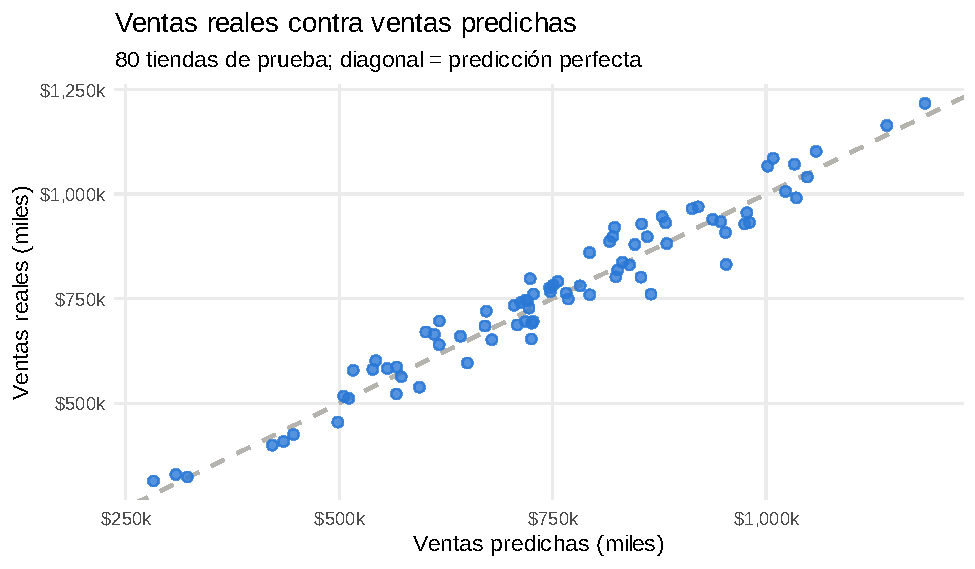
\includegraphics[width=0.9\textwidth]{m07-real-vs-predicho}
\caption{Ventas reales contra predichas por la regresión lineal en las tiendas
de prueba. Los puntos se agrupan alrededor de la diagonal, sin patrones
sistemáticos.}
\label{fig:m07-real-vs-predicho}
\end{figure}

Busca dos cosas en esta gráfica: que los puntos estén cerca de la diagonal y
que el error no dependa del tamaño (por ejemplo, que el modelo no subestime
sistemáticamente las tiendas más grandes). Aquí ambas se cumplen.

\subsection{Usar el modelo: estimar las ventas de tiendas candidatas}

\begin{rcode}
candidatas <- tibble(
  tienda     = c("Local Plaza Norte", "Local Centro Histórico",
                 "Local Sur Express"),
  zona       = c("Norte", "Centro", "Sur"),
  tamano_m2  = c(900, 400, 250),
  publicidad = c(80, 50, 30),
  promocion  = c(1, 0, 1),
  trafico    = c(9000, 6500, 4000)
)

predict(modelo_lm, newdata = candidatas, interval = "prediction") %>%
  as_tibble() %>%
  mutate(tienda = candidatas$tienda, .before = 1) %>%
  mutate(across(where(is.numeric), ~ round(.x)))
\end{rcode}

\begin{rsalida}
# A tibble: 3 x 4
  tienda                   fit   lwr   upr
  <chr>                  <dbl> <dbl> <dbl>
1 Local Plaza Norte       1058   958  1159
2 Local Centro Histórico   630   529   730
3 Local Sur Express        456   354   557
\end{rsalida}

\codigo{interval = "prediction"} agrega un \termino{intervalo de predicción}
del 95\%: \codigo{fit} es la estimación puntual, y \codigo{lwr} y \codigo{upr}
los límites inferior y superior. Para
el local de Plaza Norte, el modelo estima ventas de \$1{,}058 mil al mes, y con
95\% de confianza entre \$958 mil y \$1{,}159 mil. Ese rango es lo que debes
llevar a la junta: si la renta solo es rentable con ventas mayores a \$1{,}100
mil, el local es una apuesta arriesgada aunque la estimación puntual se vea
bien. El local Sur Express, con ventas esperadas de \$456 mil, probablemente
no justifica la inversión.

\subsection{Comparación con random forest}

\begin{concepto}{Árboles de decisión y random forest}
Un \termino{árbol de decisión} hace preguntas sucesivas del tipo ``¿tamaño
mayor a 700 m²?'' y en cada hoja predice el promedio de las tiendas que llegan
ahí. Un \termino{random forest} (bosque aleatorio) entrena cientos de árboles,
cada uno con una muestra distinta de tiendas y de variables, y promedia sus
predicciones. Captura relaciones no lineales e interacciones sin que tengas
que especificarlas, pero es una ``caja negra'' más difícil de explicar.
\end{concepto}

\begin{rcode}
set.seed(123)
modelo_rf_ventas <- randomForest(
  ventas ~ publicidad + tamano_m2 + trafico + promocion + zona,
  data = tiendas_ent %>% mutate(zona = factor(zona)),
  ntree = 300,          # número de árboles
  importance = TRUE     # calcular importancia de variables
)
modelo_rf_ventas
\end{rcode}

\begin{rsalida}

Call:
...
               Type of random forest: regression
                     Number of trees: 300
No. of variables tried at each split: 1

          Mean of squared residuals: 7887.08
                    % Var explained: 80.2
\end{rsalida}

El bosque reporta un error \termino{OOB} (\emph{out-of-bag}): como cada árbol
se entrena con una muestra, las tiendas que quedaron fuera de esa muestra
sirven para evaluarlo, una especie de validación cruzada gratuita. Comparemos
ambos modelos en el conjunto de prueba:

\begin{rcode}
tiendas_prueba <- tiendas_prueba %>%
  mutate(pred_rf = predict(modelo_rf_ventas,
                           newdata = tiendas_prueba %>%
                             mutate(zona = factor(zona))))

bind_rows(
  metricas_regresion(tiendas_prueba$ventas, tiendas_prueba$pred_lm) %>%
    mutate(modelo = "Regresión lineal", .before = 1),
  metricas_regresion(tiendas_prueba$ventas, tiendas_prueba$pred_rf) %>%
    mutate(modelo = "Random forest", .before = 1)
) %>%
  mutate(across(where(is.numeric), ~ round(.x, 3)))
\end{rcode}

\begin{rsalida}
# A tibble: 2 x 5
  modelo             MAE  RMSE  MAPE    R2
  <chr>            <dbl> <dbl> <dbl> <dbl>
1 Regresión lineal  37.2  45.1  5.04 0.947
2 Random forest     67.7  85.3 10.5  0.809
\end{rsalida}

La regresión lineal gana con claridad: MAE de 37.2 contra 67.7 del random
forest, y R² de 0.947 contra 0.809. El bosque explica el 80.2\% de la varianza
según su estimación OOB, muy parecido a lo que obtuvo en la prueba (0.809): el
OOB es un buen adelanto del desempeño real.

\begin{negocio}{El modelo más sofisticado no siempre gana}
En esta simulación la relación es lineal por construcción, así que la
regresión lineal es el modelo ``correcto'' y le gana al bosque aleatorio. En
datos reales con umbrales y combinaciones (por ejemplo, la promoción solo
funciona en tiendas grandes), el bosque suele ganar. Por eso la práctica
profesional es: \textbf{probar un modelo simple y uno flexible, compararlos en
datos de prueba y quedarte con el más sencillo que cumpla}. Además, la
regresión lineal te da coeficientes que la dirección entiende.
\end{negocio}

\begin{hazlotu}
Quita \codigo{trafico} del modelo lineal y vuelve a evaluarlo. ¿Cuánto empeora
el MAE? ¿Cómo cambia el coeficiente de \codigo{tamano\_m2}? (Pista: al no estar
el tráfico, el tamaño absorbe parte de su efecto, porque ambas variables están
relacionadas.)
\end{hazlotu}

% ============================================================================
\section{Caso 3: clasificación para predecir el abandono de clientes}
\label{sec:m7-churn}

\begin{ejemplo}{¿A quién llama primero el equipo de retención?}
Una empresa de suscripción (piensa en un club de compras con membresía
mensual, un servicio de internet o un gimnasio) pierde cada mes a una parte de
sus clientes. El equipo de retención puede llamar a 150 clientes por semana y
ofrecerles un descuento. La pregunta: \emph{¿qué clientes tienen mayor
probabilidad de irse y, por lo tanto, a quiénes conviene llamar primero?} Es un
problema de \textbf{clasificación}: la respuesta es ``se va'' o ``se queda''.
\end{ejemplo}

El \termino{churn} (abandono, deserción o cancelación) es la proporción de
clientes que dejan de serlo en un periodo. Retener a un cliente suele costar
mucho menos que conseguir uno nuevo, por eso los modelos de churn son de los
más rentables en BI.

\subsection{Datos simulados de clientes}

Simulamos 2{,}000 clientes con variables típicas de un sistema de
suscripciones. El abandono se genera con reglas de negocio realistas: aumenta
con las quejas y los pagos tardíos, es mayor en los primeros meses, y disminuye
con la antigüedad, el uso del servicio y los planes más completos. El
\textbf{género y la edad no influyen} (los incluimos para una discusión de
ética más adelante).

\begin{rcode}
set.seed(123)
n_clientes <- 2000
clientes_churn <- tibble(
  cliente_id       = sprintf("C%04d", 1:n_clientes),
  antiguedad_meses = sample(1:72, n_clientes, replace = TRUE),
  plan             = sample(c("Básico", "Estándar", "Premium"),
                            n_clientes, replace = TRUE,
                            prob = c(0.5, 0.3, 0.2)),
  uso_mensual      = rpois(n_clientes, 8),    # visitas/usos al mes
  quejas_6m        = rpois(n_clientes, 0.8),  # quejas últimos 6 meses
  pagos_tardios    = rpois(n_clientes, 0.4),  # pagos atrasados en el año
  genero           = sample(c("F", "M"), n_clientes, replace = TRUE),
  edad             = sample(18:70, n_clientes, replace = TRUE)
) %>%
  mutate(
    # "Verdad" oculta: puntaje de riesgo (el modelo no la verá)
    efecto_plan = case_when(plan == "Básico"   ~ 0,
                            plan == "Estándar" ~ -0.6,
                            TRUE               ~ -1.3),
    riesgo = 2.0 - 0.05 * antiguedad_meses +
      1.0 * (antiguedad_meses <= 6) + 1.0 * quejas_6m -
      0.35 * uso_mensual + 0.8 * pagos_tardios + efecto_plan,
    prob_real = plogis(riesgo),               # convierte a probabilidad
    churn = if_else(runif(n_clientes) < prob_real, "Si", "No"),
    churn = factor(churn, levels = c("No", "Si")),
    plan  = factor(plan, levels = c("Básico", "Estándar", "Premium")),
    cuota_mensual = case_when(plan == "Básico"   ~ 199,
                              plan == "Estándar" ~ 349,
                              TRUE               ~ 599)
  ) %>%
  select(-efecto_plan, -riesgo, -prob_real)

glimpse(clientes_churn)
clientes_churn %>% count(churn) %>% mutate(pct = round(100 * n / sum(n), 1))
\end{rcode}

\begin{rsalida}
Rows: 2,000
Columns: 10
$ cliente_id       <chr> "C0001", "C0002", "C0003", "C0004", "C0005"~
$ antiguedad_meses <int> 31, 51, 14, 67, 42, 50, 43, 14, 25, 69, 57,~
$ plan             <fct> Estándar, Premium, Premium, Estándar, Básic~
$ uso_mensual      <int> 9, 8, 5, 14, 11, 14, 8, 10, 10, 8, 8, 9, 8,~
$ quejas_6m        <int> 1, 0, 0, 2, 1, 1, 1, 0, 0, 1, 0, 0, 3, 0, 0~
$ pagos_tardios    <int> 0, 3, 0, 1, 0, 0, 1, 0, 0, 0, 1, 1, 0, 0, 1~
$ genero           <chr> "M", "F", "M", "M", "F", "M", "M", "F", "M"~
$ edad             <int> 58, 44, 27, 57, 19, 43, 48, 36, 67, 18, 40,~
$ churn            <fct> No, No, No, No, No, No, No, No, No, No, No,~
$ cuota_mensual    <dbl> 349, 599, 599, 349, 199, 199, 349, 199, 349~
# A tibble: 2 x 3
  churn     n   pct
  <fct> <int> <dbl>
1 No     1545  77.2
2 Si      455  22.8
\end{rsalida}

\codigo{glimpse()} muestra las 10 columnas: 7 predictoras, el identificador,
la cuota mensual (que usaremos para calcular el valor del cliente) y la
variable objetivo \codigo{churn}. De los 2{,}000 clientes, 455 (22.8\%) se
fueron. Es una clase \termino{desbalanceada}: los que se quedan son más de
tres veces los que se van. Tenlo presente al leer la exactitud.

\begin{consejo}
Convierte la variable objetivo a \codigo{factor} con los niveles en un orden
explícito: \codigo{levels = c("No", "Si")}. Así R sabe que ``Si'' es la clase
de interés (la segunda), y \codigo{glm()} modelará la probabilidad de ``Si''.
Evitamos la tilde en ``Si'' para no tener problemas con nombres de columnas que
generan algunas funciones.
\end{consejo}

Antes de modelar, una mirada exploratoria rápida (como en el
Módulo~\ref{cap:eda}): ¿cómo cambia la tasa de abandono con las quejas?

\begin{rcode}
clientes_churn %>%
  mutate(quejas = if_else(quejas_6m >= 3, "3 o más",
                          as.character(quejas_6m))) %>%
  group_by(quejas) %>%
  summarise(clientes = n(),
            tasa_churn = round(100 * mean(churn == "Si"), 1),
            .groups = "drop")
\end{rcode}

\begin{rsalida}
# A tibble: 4 x 3
  quejas  clientes tasa_churn
  <chr>      <int>      <dbl>
1 0            903       13.4
2 1            747       22.6
3 2            270       42.6
4 3 o más       80       62.5
\end{rsalida}

La relación es clarísima: sin quejas, solo 13.4\% abandona; con 3 o más
quejas, 62.5\%. Este tipo de tabla es la mejor forma de verificar, antes de
modelar, que hay señal en los datos.

Dividimos en entrenamiento (70\%) y prueba (30\%) de forma
\textbf{estratificada} con la función \codigo{createDataPartition()}, para que ambos
conjuntos tengan la misma proporción de abandono:

\begin{rcode}
set.seed(123)
filas_ent <- createDataPartition(clientes_churn$churn, p = 0.7,
                                 list = FALSE)
churn_ent    <- clientes_churn[filas_ent, ]
churn_prueba <- clientes_churn[-filas_ent, ]

# Misma proporción de "Si" en ambos conjuntos
round(prop.table(table(churn_ent$churn)), 3)
round(prop.table(table(churn_prueba$churn)), 3)
\end{rcode}

\begin{rsalida}

   No    Si 
0.772 0.228 

   No    Si 
0.773 0.227 
\end{rsalida}

\subsection{Regresión logística}

\begin{concepto}{Regresión logística}
La \termino{regresión logística} es la ``regresión lineal de la
clasificación''. En lugar de predecir un número cualquiera, predice una
\textbf{probabilidad} entre 0 y 1 (por ejemplo, 0.73 = 73\% de probabilidad de
abandono). En R se ajusta con \codigo{glm(..., family = binomial)}. Es rápida,
estable y, sobre todo, \textbf{explicable}: cada coeficiente dice cómo cambia
el riesgo.
\end{concepto}

\begin{rcode}
formula_churn <- churn ~ antiguedad_meses + plan + uso_mensual +
  quejas_6m + pagos_tardios + genero + edad

modelo_log <- glm(formula_churn, data = churn_ent, family = binomial)
summary(modelo_log)
\end{rcode}

\begin{rsalida}

Call:
glm(formula = formula_churn, family = binomial, data = churn_ent)

Coefficients:
                  Estimate Std. Error z value Pr(>|z|)    
(Intercept)       2.114728   0.385699   5.483 4.19e-08 ***
antiguedad_meses -0.054049   0.004438 -12.178  < 2e-16 ***
planEstándar     -0.448662   0.175005  -2.564   0.0104 *  
planPremium      -1.247963   0.234692  -5.317 1.05e-07 ***
uso_mensual      -0.310629   0.032282  -9.622  < 2e-16 ***
quejas_6m         1.048309   0.091879  11.410  < 2e-16 ***
pagos_tardios     0.528275   0.121604   4.344 1.40e-05 ***
generoM           0.019595   0.154767   0.127   0.8992    
edad             -0.003247   0.005179  -0.627   0.5306    
---
Signif. codes:  0 '***' 0.001 '**' 0.01 '*' 0.05 '.' 0.1 ' ' 1

(Dispersion parameter for binomial family taken to be 1)

    Null deviance: 1503.2  on 1400  degrees of freedom
Residual deviance: 1063.0  on 1392  degrees of freedom
AIC: 1081

Number of Fisher Scoring iterations: 5
\end{rsalida}

Los coeficientes de la logística están en una escala poco intuitiva
(\emph{log-odds}). Para explicarlos al negocio, conviértelos en
\termino{razones de momios} (\emph{odds ratios}) con \codigo{exp()}:

\begin{rcode}
tibble(variable   = names(coef(modelo_log)),
       odds_ratio = round(exp(coef(modelo_log)), 3)) %>%
  mutate(efecto = case_when(
    odds_ratio > 1 ~ paste0("+", round(100 * (odds_ratio - 1)), "% riesgo"),
    TRUE           ~ paste0(round(100 * (odds_ratio - 1)), "% riesgo")
  )) %>%
  filter(variable != "(Intercept)")
\end{rcode}

\begin{rsalida}
# A tibble: 8 x 3
  variable         odds_ratio efecto      
  <chr>                 <dbl> <chr>       
1 antiguedad_meses      0.947 -5% riesgo  
2 planEstándar          0.638 -36% riesgo 
3 planPremium           0.287 -71% riesgo 
4 uso_mensual           0.733 -27% riesgo 
5 quejas_6m             2.85  +185% riesgo
6 pagos_tardios         1.70  +70% riesgo 
7 generoM               1.02  +2% riesgo  
8 edad                  0.997 0% riesgo   
\end{rsalida}

\begin{concepto}{Cómo leer una razón de momios}
Los \emph{momios} (\emph{odds}) son la probabilidad de que algo pase dividida
entre la probabilidad de que no pase. Una razón de momios de 1 significa ``no
cambia el riesgo''; mayor a 1, lo aumenta; menor a 1, lo reduce. Se interpreta
\emph{por cada unidad} de la variable y manteniendo las demás constantes.
\end{concepto}

Traducido al negocio:
\begin{itemize}
  \item \textbf{Quejas:} cada queja adicional multiplica los momios de
        abandono por 2.85 (casi los triplica). Es la palanca más fuerte:
        resolver bien una queja vale mucho.
  \item \textbf{Pagos tardíos:} cada pago atrasado aumenta los momios 70\%.
        Es una señal temprana que cobranza ya tiene y puede compartir.
  \item \textbf{Uso:} cada uso adicional al mes reduce los momios 27\%. Los
        clientes que usan el servicio se quedan.
  \item \textbf{Antigüedad:} cada mes adicional reduce los momios 5\%; en un
        año, eso se acumula ($0.947^{12} \approx 0.52$, casi la mitad).
  \item \textbf{Plan:} frente al Básico, el Premium reduce los momios 71\% y
        el Estándar 36\%.
  \item \textbf{Género y edad:} razones cercanas a 1 y valores p altos (0.90
        y 0.53 en el resumen): no influyen, tal como los simulamos.
\end{itemize}
Observa también que el modelo no ``descubrió'' el riesgo extra de los primeros
6 meses, porque no le dimos una variable que lo represente; la antigüedad
lineal lo absorbe en parte. Crear variables como
\codigo{cliente\_nuevo = antiguedad\_meses <= 6} es el tipo de mejora que se
logra entendiendo el negocio (ejercicio~\ref{ej:m7-6}).

\subsection{Predicciones y matriz de confusión}

El modelo entrega probabilidades. Para convertirlas en una decisión (llamar o
no llamar) necesitamos un \termino{umbral}: si la probabilidad es mayor o igual
al umbral, clasificamos como ``Si''. Empecemos con el umbral por defecto,
0.5:

\begin{rcode}
churn_prueba <- churn_prueba %>%
  mutate(prob_log = predict(modelo_log, newdata = churn_prueba,
                            type = "response"),   # probabilidad de "Si"
         pred_log = factor(if_else(prob_log >= 0.5, "Si", "No"),
                           levels = c("No", "Si")))

churn_prueba %>%
  select(cliente_id, antiguedad_meses, quejas_6m, prob_log, pred_log,
         churn) %>%
  mutate(prob_log = round(prob_log, 3)) %>%
  head(5)

# Matriz de confusión: filas = predicción, columnas = realidad
matriz <- table(Prediccion = churn_prueba$pred_log,
                Real = churn_prueba$churn)
matriz
\end{rcode}

\begin{rsalida}
# A tibble: 5 x 6
  cliente_id antiguedad_meses quejas_6m prob_log pred_log churn
  <chr>                 <int>     <int>    <dbl> <fct>    <fct>
1 C0003                    14         0    0.181 No       No   
2 C0007                    43         1    0.154 No       No   
3 C0012                     9         0    0.119 No       No   
4 C0014                    26         0    0.224 No       No   
5 C0015                     7         0    0.416 No       Si   
          Real
Prediccion  No  Si
        No 434  69
        Si  29  67
\end{rsalida}

\begin{concepto}{Matriz de confusión}
Compara lo que el modelo predijo con lo que realmente pasó:

\begin{center}
\small
\begin{tabular}{lcc}
\toprule
 & \textbf{Real: No se fue} & \textbf{Real: Sí se fue} \\
\midrule
\textbf{Predicción: No} & Verdadero negativo (VN) & Falso negativo (FN) \\
\textbf{Predicción: Sí} & Falso positivo (FP) & Verdadero positivo (VP) \\
\bottomrule
\end{tabular}
\end{center}

\begin{itemize}
  \item \textbf{Falso positivo:} llamas a un cliente que no se iba a ir
        (desperdicias un descuento).
  \item \textbf{Falso negativo:} no llamas a un cliente que sí se va (lo
        pierdes). Suele ser el error más caro.
\end{itemize}
\end{concepto}

En nuestros 599 clientes de prueba: el modelo acertó 434 clientes que se
quedaron (VN) y 67 que se fueron (VP). Se equivocó con 29 clientes que marcó
como ``se va'' y se quedaron (FP) y, lo más grave, dejó pasar a 69 clientes que
se fueron sin que los detectara (FN). Mira también el cliente C0015 en la
tabla de arriba: tenía 41.6\% de probabilidad y sí se fue; con el umbral de 0.5
no lo habríamos llamado.

\subsection{Métricas de clasificación}
\label{sec:m7-metricas-clas}

De la matriz de confusión salen todas las métricas. Las calculamos a mano para
entender qué significa cada una:

\begin{rcode}
metricas_clasificacion <- function(prediccion, real, positivo = "Si") {
  vp <- sum(prediccion == positivo & real == positivo)
  vn <- sum(prediccion != positivo & real != positivo)
  fp <- sum(prediccion == positivo & real != positivo)
  fn <- sum(prediccion != positivo & real == positivo)
  precision    <- vp / (vp + fp)
  sensibilidad <- vp / (vp + fn)
  tibble(
    exactitud    = (vp + vn) / (vp + vn + fp + fn),
    precision    = precision,
    sensibilidad = sensibilidad,
    especificidad = vn / (vn + fp),
    F1           = 2 * precision * sensibilidad /
                   (precision + sensibilidad)
  )
}

metricas_clasificacion(churn_prueba$pred_log, churn_prueba$churn) %>%
  mutate(across(everything(), ~ round(.x, 3)))
\end{rcode}

\begin{rsalida}
# A tibble: 1 x 5
  exactitud precision sensibilidad especificidad    F1
      <dbl>     <dbl>        <dbl>         <dbl> <dbl>
1     0.836     0.698        0.493         0.937 0.578
\end{rsalida}

\begin{table}[H]
\centering
\small
\caption{Métricas de clasificación y la pregunta de negocio que responden.}
\label{tab:m7-metricas-clas}
\begin{tabularx}{\textwidth}{>{\raggedright\arraybackslash}p{2.6cm}
                              >{\raggedright\arraybackslash}p{3.3cm}
                              >{\raggedright\arraybackslash}X}
\toprule
\textbf{Métrica} & \textbf{Fórmula} & \textbf{Pregunta que responde} \\
\midrule
Exactitud (\emph{accuracy}) & $(VP + VN) / \text{total}$ &
  ¿Qué proporción de clientes clasificamos bien? Engañosa si una clase es
  rara. \\
Precisión (\emph{precision}) & $VP / (VP + FP)$ &
  De los clientes que marcamos como ``se va'', ¿cuántos realmente se iban?
  (eficiencia de las llamadas). \\
Sensibilidad (\emph{recall}) & $VP / (VP + FN)$ &
  De los clientes que se fueron, ¿a cuántos detectamos? (cobertura). \\
Especificidad & $VN / (VN + FP)$ &
  De los que se quedaron, ¿a cuántos dejamos tranquilos? \\
F1 & $2 \cdot \dfrac{\text{prec.} \cdot \text{sens.}}{\text{prec.} + \text{sens.}}$ &
  Equilibrio entre precisión y sensibilidad en un solo número. \\
\bottomrule
\end{tabularx}
\end{table}

La exactitud es de 83.6\%, que suena bien, pero la sensibilidad es de solo
49.3\%: con el umbral de 0.5 detectamos a menos de la mitad de los clientes que
se van. La precisión de 69.8\% dice que de cada 10 llamadas, 7 serían a
clientes realmente en riesgo. Recuerda que predecir ``nadie se va'' ya daría
77.3\% de exactitud (la proporción de ``No'' en la prueba), así que la exactitud
por sí sola dice poco (sección~\ref{sec:m7-errores}).

\subsection{Curva ROC y AUC}

Cada umbral produce una matriz de confusión distinta. La \termino{curva ROC}
muestra todos los umbrales a la vez: en el eje horizontal, la tasa de falsos
positivos ($1 -$ especificidad); en el vertical, la sensibilidad. El
\termino{AUC} (área bajo la curva) resume la curva en un número: la
probabilidad de que, al tomar un cliente que se fue y uno que se quedó al azar,
el modelo le asigne mayor riesgo al que se fue. Un AUC de 0.5 es adivinar con
una moneda; 1 es perfecto; en churn, de 0.75 a 0.85 ya es un buen modelo.

Calculamos la curva a mano, probando 101 umbrales:

\begin{rcode}
curva_roc <- function(prob, real, positivo = "Si") {
  map_dfr(seq(0, 1, by = 0.01), function(u) {
    pred <- prob >= u
    tibble(umbral = u,
           sensibilidad = sum(pred & real == positivo) /
                          sum(real == positivo),
           tasa_fp = sum(pred & real != positivo) / sum(real != positivo))
  })
}

# AUC como probabilidad de ordenar bien un par (positivo, negativo)
calcular_auc <- function(prob, real, positivo = "Si") {
  p_pos <- prob[real == positivo]
  p_neg <- prob[real != positivo]
  mean(outer(p_pos, p_neg, ">") + 0.5 * outer(p_pos, p_neg, "=="))
}

roc_log <- curva_roc(churn_prueba$prob_log, churn_prueba$churn)
auc_log <- calcular_auc(churn_prueba$prob_log, churn_prueba$churn)
round(auc_log, 3)
# round() evita problemas de precisión al comparar decimales
roc_log %>% filter(round(umbral, 2) %in% c(0.1, 0.2, 0.3, 0.5, 0.7))
\end{rcode}

\begin{rsalida}
[1] 0.86
# A tibble: 5 x 3
  umbral sensibilidad tasa_fp
   <dbl>        <dbl>   <dbl>
1    0.1        0.941  0.460 
2    0.2        0.801  0.298 
3    0.3        0.691  0.173 
4    0.5        0.493  0.0626
5    0.7        0.331  0.0151
\end{rsalida}

El AUC es de 0.86: si tomas al azar un cliente que se fue y uno que se quedó,
en 86\% de los casos el modelo le asigna más riesgo al que se fue. La tabla
muestra el dilema del umbral: con 0.5 detectamos 49.3\% de los que se van
molestando solo a 6.3\% de los que se quedan; con 0.2 detectamos 80.1\%, pero
molestamos a 29.8\%; con 0.1, 94.1\% y 46\%. En el otro extremo, con 0.7 casi no molestamos a nadie (1.5\%), pero solo
detectamos a un tercio (33.1\%) de los que se van.

\begin{rcode}
grafico_roc <- ggplot(roc_log, aes(x = tasa_fp, y = sensibilidad)) +
  geom_abline(slope = 1, intercept = 0, color = color_gris,
              linetype = "dashed", linewidth = 0.8) +
  geom_path(color = color_principal, linewidth = 0.8) +
  geom_point(data = filter(roc_log, umbral %in% c(0.2, 0.5)),
             color = color_resalte, size = 3) +
  geom_text(data = filter(roc_log, umbral %in% c(0.2, 0.5)),
            aes(label = paste("umbral", umbral)), color = color_resalte,
            hjust = -0.2, vjust = 1.2, size = 3.5) +
  annotate("text", x = 0.75, y = 0.25,
           label = paste("AUC =", round(auc_log, 3)), size = 4.5) +
  scale_x_continuous(labels = scales::percent) +
  scale_y_continuous(labels = scales::percent) +
  coord_equal() +
  labs(title = "Curva ROC de la regresión logística",
       subtitle = "Clientes de prueba; la diagonal equivale a adivinar",
       x = "Tasa de falsos positivos (1 - especificidad)",
       y = "Sensibilidad") +
  theme_minimal() +
  theme(panel.grid.minor = element_blank())
grafico_roc
\end{rcode}

\begin{figure}[H]
\centering
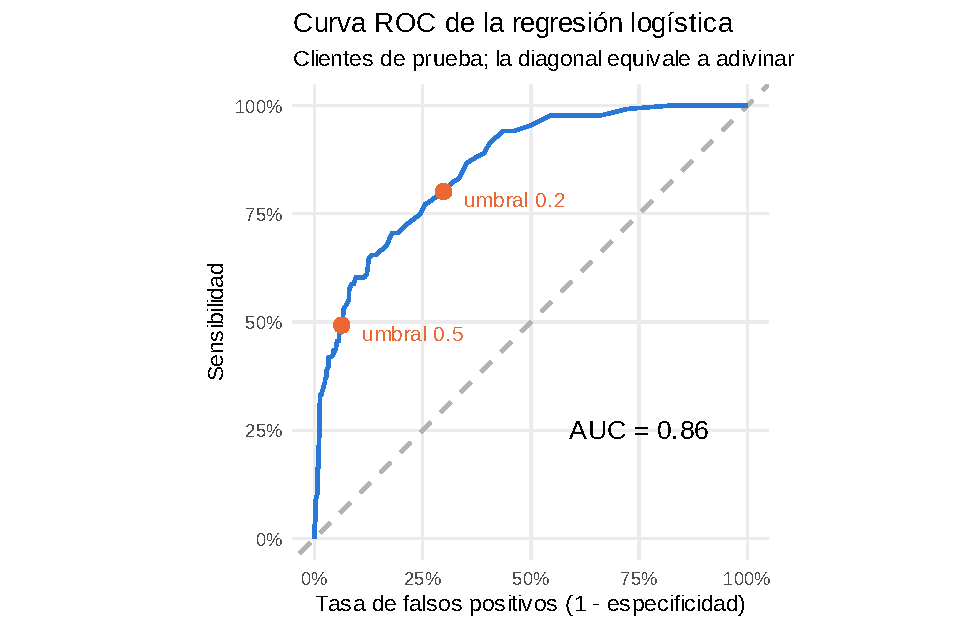
\includegraphics[width=0.9\textwidth]{m07-roc}
\caption{Curva ROC del modelo de abandono. Bajar el umbral de 0.5 a 0.2 sube
mucho la sensibilidad a cambio de más falsos positivos.}
\label{fig:m07-roc}
\end{figure}

\subsection{Elegir el umbral según el costo de negocio}
\label{sec:m7-umbral}

El umbral de 0.5 no tiene nada de especial. La decisión correcta depende de
cuánto cuesta cada error. Supongamos estos valores (en pesos):

\begin{table}[H]
\centering
\small
\caption{Supuestos de costos para la campaña de retención.}
\label{tab:m7-costos}
\begin{tabularx}{\textwidth}{>{\raggedright\arraybackslash}p{4.2cm}
                              >{\raggedright\arraybackslash}X r}
\toprule
\textbf{Resultado} & \textbf{Qué pasa} & \textbf{Costo} \\
\midrule
Verdadero positivo (VP) & Llamamos y ofrecemos descuento; la mitad de ellos se
  queda y la otra mitad se va de todos modos. & $300 + 0.5 \times 3{,}000 = 1{,}800$ \\
Falso positivo (FP) & Damos un descuento a quien no se iba a ir. & 300 \\
Falso negativo (FN) & No llamamos y el cliente se va: perdemos su margen de
  un año. & 3{,}000 \\
Verdadero negativo (VN) & No hacemos nada y el cliente se queda. & 0 \\
\bottomrule
\end{tabularx}
\end{table}

Con esos costos, calculamos el costo total de la campaña para cada umbral y
buscamos el mínimo:

\begin{rcode}
costo_vp <- 300 + 0.5 * 3000   # descuento + clientes que igual se van
costo_fp <- 300                # descuento desperdiciado
costo_fn <- 3000               # cliente perdido sin intentar retenerlo

costos_umbral <- map_dfr(seq(0.05, 0.95, by = 0.05), function(u) {
  pred <- churn_prueba$prob_log >= u
  real <- churn_prueba$churn == "Si"
  tibble(umbral = u,
         llamadas = sum(pred),
         vp = sum(pred & real), fp = sum(pred & !real),
         fn = sum(!pred & real),
         costo_total = vp * costo_vp + fp * costo_fp + fn * costo_fn)
})

costos_umbral %>% arrange(costo_total) %>% head(3)
costos_umbral %>% filter(umbral %in% c(0.5, 0.95))
\end{rcode}

\begin{rsalida}
# A tibble: 3 x 6
  umbral llamadas    vp    fp    fn costo_total
   <dbl>    <int> <int> <int> <int>       <dbl>
1   0.15      294   120   174    16      316200
2   0.1       341   128   213     8      318300
3   0.2       247   109   138    27      318600
# A tibble: 2 x 6
  umbral llamadas    vp    fp    fn costo_total
   <dbl>    <int> <int> <int> <int>       <dbl>
1   0.5        96    67    29    69      336300
2   0.95        4     4     0   132      403200
\end{rsalida}

Con estos costos, el mejor umbral es 0.15: llamaríamos a 294 clientes de
prueba, detectaríamos a 120 de los 136 que se van y el costo total sería
\$316{,}200. Con el umbral por defecto de 0.5 el costo sube a \$336{,}300,
y casi sin llamar a nadie (umbral 0.95) a \$403{,}200. Elegir bien el umbral
ahorra \$20{,}100 en solo 599 clientes; escalado a una cartera de 100{,}000
clientes, son más de 3 millones de pesos.

\begin{rcode}
grafico_costos <- ggplot(costos_umbral, aes(umbral, costo_total)) +
  geom_line(color = color_principal, linewidth = 0.8) +
  geom_point(color = color_principal, size = 1.5) +
  geom_point(data = slice_min(costos_umbral, costo_total, n = 1),
             color = color_resalte, size = 4) +
  scale_y_continuous(labels = scales::dollar) +
  labs(title = "Costo total de la campaña según el umbral",
       subtitle = "Clientes de prueba; en naranja, el umbral óptimo",
       x = "Umbral de probabilidad para llamar al cliente",
       y = "Costo total") +
  theme_minimal() +
  theme(panel.grid.minor = element_blank())
grafico_costos
\end{rcode}

\begin{figure}[H]
\centering
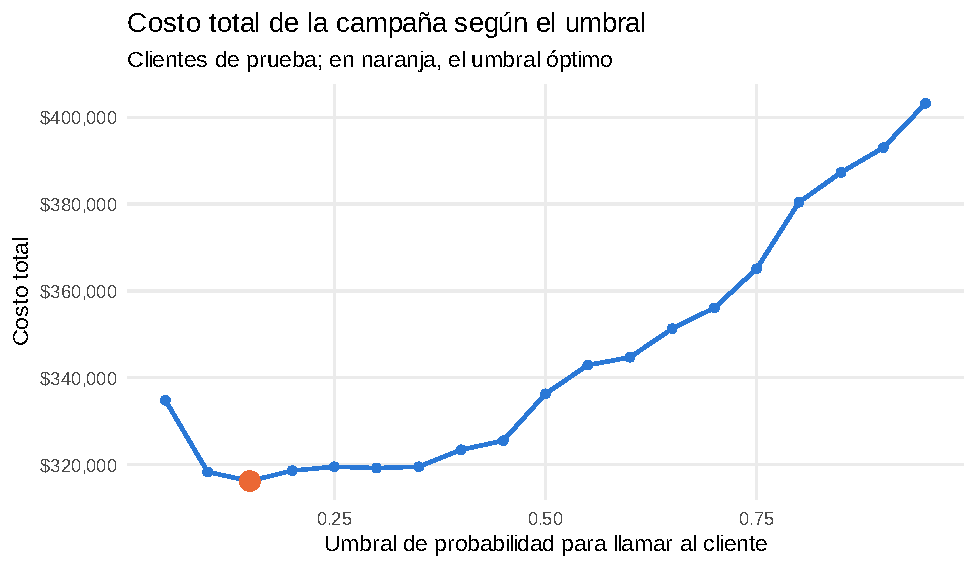
\includegraphics[width=0.9\textwidth]{m07-costo-umbral}
\caption{Costo total de la campaña de retención para cada umbral. Con errores
de costos tan distintos, conviene un umbral mucho más bajo que 0.5.}
\label{fig:m07-costo-umbral}
\end{figure}

\begin{negocio}{El umbral es una decisión de negocio, no técnica}
Cuando el costo de perder un cliente es mucho mayor que el de un descuento, el
umbral óptimo baja: conviene llamar a más gente aunque muchos no se fueran a ir.
Si el equipo de retención tiene capacidad limitada (150 llamadas por semana),
el umbral lo fija la capacidad: llamas a los 150 de mayor probabilidad. Lo
importante es que el modelo \emph{ordena} bien a los clientes por riesgo, y
eso lo mide el AUC.
\end{negocio}

\begin{hazlotu}
Repite el cálculo de costos suponiendo que el descuento cuesta \$800 en lugar
de \$300. ¿Sube o baja el umbral óptimo? ¿Por qué?
\end{hazlotu}

\subsection{Árbol de decisión con \texorpdfstring{\codigo{rpart}}{rpart}}

Un \termino{árbol de decisión} produce reglas del tipo ``si antigüedad < 20
meses y uso < 8, entonces riesgo alto''. Su gran ventaja es que cualquier
gerente las entiende. Para que el árbol sea legible limitamos su complejidad
con el parámetro \codigo{cp} (\emph{complexity parameter}): un corte solo se
hace si mejora el ajuste al menos en esa proporción.

\begin{rcode}
set.seed(123)
modelo_arbol <- rpart(formula_churn, data = churn_ent, method = "class",
                      control = rpart.control(cp = 0.02))
modelo_arbol
\end{rcode}

\begin{rsalida}
n= 1401 

node), split, n, loss, yval, (yprob)
      * denotes terminal node

 1) root 1401 319 No (0.7723055 0.2276945)  
   2) antiguedad_meses>=20.5 1014 151 No (0.8510848 0.1489152) *
   3) antiguedad_meses< 20.5 387 168 No (0.5658915 0.4341085)  
     6) uso_mensual>=7.5 211  63 No (0.7014218 0.2985782) *
     7) uso_mensual< 7.5 176  71 Si (0.4034091 0.5965909)  
      14) quejas_6m< 1.5 134  64 Si (0.4776119 0.5223881)  
        28) plan=Estándar,Premium 66  25 No (0.6212121 0.3787879) *
        29) plan=Básico 68  23 Si (0.3382353 0.6617647) *
      15) quejas_6m>=1.5 42   7 Si (0.1666667 0.8333333) *
\end{rsalida}

Cada línea es un nodo: número, regla, clientes que llegan, clientes mal
clasificados, clase predicha y proporciones (No, Si). Las hojas se marcan con
\codigo{*}. Leídas como reglas de negocio:

\begin{enumerate}
  \item \textbf{Antigüedad $\geq$ 21 meses} (1{,}014 clientes): riesgo bajo,
        14.9\% abandona.
  \item \textbf{Antigüedad < 21 meses y uso $\geq$ 8} (211): riesgo medio,
        29.9\%.
  \item \textbf{Antigüedad < 21, uso < 8 y 2 o más quejas} (42): riesgo muy
        alto, 83.3\%.
  \item \textbf{Antigüedad < 21, uso < 8, menos de 2 quejas y plan Básico}
        (68): riesgo alto, 66.2\%.
  \item Lo mismo pero con plan Estándar o Premium (66): 37.9\%.
\end{enumerate}

Estas reglas se pueden pegar tal cual en una presentación o programar en SQL.
Coinciden con lo que dijo la logística: antigüedad, uso, quejas y plan.

Para dibujar el árbol, el paquete \paquete{rpart.plot} produce diagramas muy
claros. No viene con R; si lo instalas, bastan dos líneas:

\begin{rnoejecutar}
install.packages("rpart.plot")
library(rpart.plot)
rpart.plot(modelo_arbol, type = 4, extra = 104,
           box.palette = "BuOr", main = "Árbol de abandono")
\end{rnoejecutar}

Sin paquetes extra, \codigo{plot(modelo\_arbol); text(modelo\_arbol)} dibuja
una versión sencilla con gráficos base. ¿Qué variables usa más el árbol?

\begin{rcode}
round(modelo_arbol$variable.importance, 1)

churn_prueba <- churn_prueba %>%
  mutate(prob_arbol = predict(modelo_arbol, newdata = churn_prueba,
                              type = "prob")[, "Si"])
round(calcular_auc(churn_prueba$prob_arbol, churn_prueba$churn), 3)
\end{rcode}

\begin{rsalida}
antiguedad_meses      uso_mensual        quejas_6m             plan 
            46.1             17.4              7.0              5.4 
            edad           genero    pagos_tardios 
             0.6              0.4              0.2 
[1] 0.674
\end{rsalida}

La antigüedad es, por mucho, la variable más importante para el árbol,
seguida por el uso. Pero su AUC en prueba es de solo 0.674, bastante peor que
el 0.86 de la logística: con apenas 5 hojas, el árbol asigna la misma
probabilidad a cientos de clientes y no puede ordenarlos con detalle. Es el
precio de la simplicidad.

\subsection{Random forest}

\begin{rcode}
set.seed(123)
modelo_rf <- randomForest(formula_churn, data = churn_ent,
                          ntree = 300, importance = TRUE)
modelo_rf
\end{rcode}

\begin{rsalida}

Call:
...
               Type of random forest: classification
                     Number of trees: 300
No. of variables tried at each split: 2

        OOB estimate of  error rate: 19.49%
Confusion matrix:
     No  Si class.error
No 1008  74  0.06839187
Si  199 120  0.62382445
\end{rsalida}

El error OOB es de 19.5\%, pero la matriz de confusión OOB revela el mismo
problema de antes: el bosque clasifica bien a los que se quedan (6.8\% de error)
y mal a los que se van (62.4\% de error), porque usa el umbral de 0.5 por
defecto. Como vimos, para churn conviene trabajar con las probabilidades y
elegir el umbral.

\begin{rcode}
importancia_rf <- importance(modelo_rf) %>%
  as.data.frame() %>%
  rownames_to_column("variable") %>%
  as_tibble() %>%
  select(variable, MeanDecreaseAccuracy) %>%
  arrange(desc(MeanDecreaseAccuracy))
importancia_rf %>% mutate(MeanDecreaseAccuracy =
                            round(MeanDecreaseAccuracy, 1))

grafico_importancia <- ggplot(importancia_rf,
       aes(x = MeanDecreaseAccuracy,
           y = reorder(variable, MeanDecreaseAccuracy))) +
  geom_col(fill = color_principal, width = 0.7) +
  labs(title = "¿Qué variables usa el bosque para predecir el abandono?",
       subtitle = "Pérdida de exactitud al desordenar cada variable",
       x = "Importancia (disminución media de exactitud)", y = NULL) +
  theme_minimal() +
  theme(panel.grid.minor = element_blank(),
        panel.grid.major.y = element_blank())
grafico_importancia
\end{rcode}

\begin{rsalida}
# A tibble: 7 x 2
  variable         MeanDecreaseAccuracy
  <chr>                           <dbl>
1 antiguedad_meses                 32.6
2 quejas_6m                        31.3
3 uso_mensual                      23  
4 plan                              6.9
5 pagos_tardios                     4.7
6 genero                            3  
7 edad                              2.4
\end{rsalida}

\begin{figure}[H]
\centering
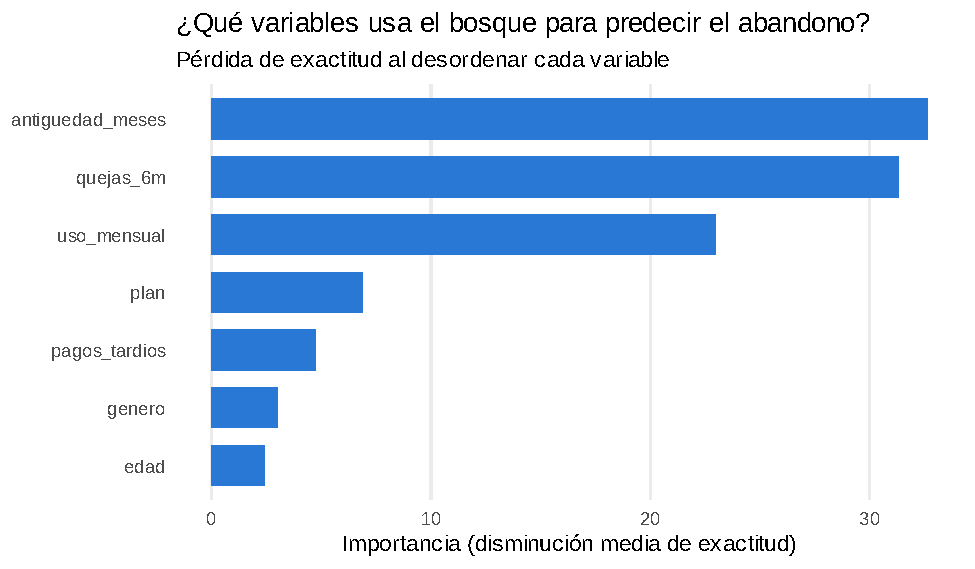
\includegraphics[width=0.9\textwidth]{m07-importancia}
\caption{Importancia de variables del random forest. Antigüedad, quejas y uso
dominan; género y edad no aportan.}
\label{fig:m07-importancia}
\end{figure}

\begin{concepto}{Importancia por permutación}
\codigo{MeanDecreaseAccuracy} responde: ``si desordeno al azar los valores de
esta variable (rompiendo su relación con el abandono), ¿cuánto empeora el
modelo?''. Si casi no empeora, la variable no aportaba. Es una forma de abrir
un poco la caja negra.
\end{concepto}

El bosque coincide con los demás modelos: antigüedad (32.6), quejas (31.3) y
uso (23.0) son las variables clave; plan y pagos tardíos aportan algo; género y
edad aportan muy poco. Que distintos algoritmos coincidan en las variables
importantes da confianza en el hallazgo.

\subsection{Comparar modelos con \texorpdfstring{\paquete{caret}}{caret}}

Hasta ahora cada algoritmo tenía su propia sintaxis. El paquete
\paquete{caret} ofrece una interfaz común, \codigo{train()}, para más de 200
algoritmos, y se encarga de la validación cruzada y del ajuste de parámetros.
Comparemos los tres modelos con validación cruzada de 5 pliegues usando el AUC
(que \paquete{caret} llama \codigo{ROC}) como criterio.

\begin{rcode}
# caret toma como clase positiva el PRIMER nivel del factor
churn_ent_caret <- churn_ent %>%
  mutate(churn = factor(churn, levels = c("Si", "No")))

control_cv <- trainControl(
  method = "cv", number = 5,           # validación cruzada de 5 pliegues
  classProbs = TRUE,                   # calcular probabilidades
  summaryFunction = twoClassSummary    # reportar ROC, Sens y Spec
)

set.seed(123)
cv_log <- train(formula_churn, data = churn_ent_caret, method = "glm",
                family = binomial, trControl = control_cv, metric = "ROC")
set.seed(123)
cv_arbol <- train(formula_churn, data = churn_ent_caret,
                  method = "rpart", trControl = control_cv,
                  metric = "ROC", tuneLength = 5)   # prueba 5 valores de cp
set.seed(123)
cv_rf <- train(formula_churn, data = churn_ent_caret, method = "rf",
               trControl = control_cv, metric = "ROC", ntree = 200,
               tuneGrid = data.frame(mtry = 2:4))   # variables por corte

cv_rf
\end{rcode}

\begin{rsalida}
Random Forest 

1401 samples
   7 predictor
   2 classes: 'Si', 'No' 

No pre-processing
Resampling: Cross-Validated (5 fold) 
Summary of sample sizes: 1121, 1121, 1120, 1122, 1120 
Resampling results across tuning parameters:

  mtry  ROC        Sens       Spec     
  2     0.8187057  0.3446925  0.9454600
  3     0.8115210  0.4198413  0.9149727
  4     0.8048380  0.4293155  0.9094342

ROC was used to select the optimal model using the largest value.
The final value used for the model was mtry = 2.
\end{rsalida}

\codigo{train()} probó tres valores de \codigo{mtry} (cuántas variables
considera el bosque en cada corte) y eligió el de mayor AUC promedio en los 5
pliegues. Ahora juntamos los tres modelos en una tabla:

\begin{rcode}
comparacion <- resamples(list(Logistica = cv_log, Arbol = cv_arbol,
                              RandomForest = cv_rf))

summary(comparacion)$statistics$ROC[, c("Min.", "Mean", "Max.")] %>%
  round(3)
\end{rcode}

\begin{rsalida}
              Min.  Mean  Max.
Logistica    0.828 0.843 0.882
Arbol        0.657 0.691 0.735
RandomForest 0.795 0.819 0.842
\end{rsalida}

Y confirmamos con los datos de prueba, que ningún modelo ha visto:

\begin{rcode}
churn_prueba <- churn_prueba %>%
  mutate(prob_rf = predict(modelo_rf, newdata = churn_prueba,
                           type = "prob")[, "Si"])

tibble(
  modelo = c("Regresión logística", "Árbol de decisión",
             "Random forest"),
  auc_prueba = c(calcular_auc(churn_prueba$prob_log, churn_prueba$churn),
                 calcular_auc(churn_prueba$prob_arbol, churn_prueba$churn),
                 calcular_auc(churn_prueba$prob_rf, churn_prueba$churn))
) %>%
  mutate(auc_prueba = round(auc_prueba, 3)) %>%
  arrange(desc(auc_prueba))
\end{rcode}

\begin{rsalida}
# A tibble: 3 x 2
  modelo              auc_prueba
  <chr>                    <dbl>
1 Regresión logística      0.86 
2 Random forest            0.846
3 Árbol de decisión        0.674
\end{rsalida}

Validación cruzada y prueba cuentan la misma historia: la regresión logística
gana (AUC de 0.843 en validación cruzada y 0.86 en prueba), seguida muy de
cerca por el random forest (0.819 y 0.846), mientras que el árbol sencillo
queda muy atrás (0.691 y 0.674). Como en la regresión de ventas, la relación
simulada es casi lineal y el modelo simple gana. Con la logística tenemos,
además, odds ratios que el negocio entiende: es el modelo que llevaríamos a
producción.

\subsection{Del modelo a la acción: lista priorizada de clientes en riesgo}

El entregable final para el equipo de retención no es un AUC: es una
\textbf{lista de clientes ordenada por prioridad}. Una buena práctica es
ordenar por \termino{pérdida esperada}: probabilidad de abandono $\times$
valor del cliente (aquí, su cuota de un año). Así, un cliente Premium con 50\%
de riesgo puede ir antes que uno Básico con 70\%.

\begin{rcode}
lista_retencion <- churn_prueba %>%
  mutate(valor_anual     = cuota_mensual * 12,
         perdida_esperada = prob_log * valor_anual) %>%
  arrange(desc(perdida_esperada)) %>%
  mutate(prioridad = row_number()) %>%
  select(prioridad, cliente_id, plan, quejas_6m, prob_log,
         perdida_esperada)

lista_retencion %>%
  mutate(prob_log = round(prob_log, 2),
         perdida_esperada = round(perdida_esperada)) %>%
  head(8)
\end{rcode}

\begin{rsalida}
# A tibble: 8 x 6
  prioridad cliente_id plan     quejas_6m prob_log perdida_esperada
      <int> <chr>      <fct>        <int>    <dbl>            <dbl>
1         1 C0259      Premium          2     0.88             6313
2         2 C1336      Premium          2     0.87             6261
3         3 C0609      Premium          1     0.67             4838
4         4 C1058      Premium          1     0.66             4768
5         5 C1912      Premium          2     0.57             4085
6         6 C1072      Estándar         3     0.97             4049
7         7 C1354      Premium          2     0.56             4029
8         8 C0795      Premium          2     0.55             3973
\end{rsalida}

Los primeros lugares los ocupan clientes Premium con probabilidad alta: su
cuota de \$599 hace que perderlos cueste más. El cliente C1072 tiene la mayor
probabilidad de la tabla (0.97), pero como es Estándar queda en el sexto lugar.
Esta lista, exportada a CSV cada semana, es lo que realmente usa el call
center (sección~\ref{sec:m7-produccion}).

\begin{hazlotu}
Agrega a la lista una columna \codigo{motivo\_principal} con
\codigo{case\_when()}: ``Quejas'' si \codigo{quejas\_6m >= 2}, ``Cliente
nuevo'' si \codigo{antiguedad\_meses <= 6}, ``Poco uso'' si
\codigo{uso\_mensual < 5} y ``Otro'' en los demás casos. El equipo de retención
podrá adaptar su guion según el motivo.
\end{hazlotu}

% ============================================================================
\section{Caso 4: pronóstico de demanda con series de tiempo}
\label{sec:m7-series}

\begin{ejemplo}{¿Cuántas unidades pedimos para diciembre?}
El área de compras de la categoría de electrónica debe colocar sus pedidos con
dos meses de anticipación. Si pide de menos en noviembre y diciembre (Buen Fin
y Navidad) pierde ventas; si pide de más, se queda con inventario que en enero
nadie quiere. La pregunta: \emph{¿cuántas unidades venderemos cada mes del
próximo año, y con qué margen de error?}
\end{ejemplo}

Una \termino{serie de tiempo} es una secuencia de mediciones ordenadas en el
tiempo a intervalos regulares (ventas diarias, demanda mensual). Sus
componentes típicos son:

\begin{itemize}
  \item \termino{Tendencia}: la dirección de largo plazo (el negocio crece).
  \item \termino{Estacionalidad}: patrones que se repiten cada año (picos en
        noviembre y diciembre, caída en enero y febrero).
  \item \termino{Ruido} (componente irregular): lo que queda, variaciones que
        no siguen un patrón.
\end{itemize}

\subsection{Datos: cinco años de ventas mensuales}

Las ventas del curso solo cubren 2023 y son aleatorias, así que simulamos 5
años (2021--2025) de unidades vendidas por mes con una tendencia creciente
(unas 15 unidades más cada mes), una estacionalidad típica del retail mexicano
(picos de 15\% y 32\% sobre lo normal en noviembre y diciembre) y 3\% de ruido.

\begin{rcode}
set.seed(123)
meses <- seq(as.Date("2021-01-01"), as.Date("2025-12-01"), by = "month")
n_meses <- length(meses)   # 60 meses

# Factor estacional de cada mes (1 = mes normal)
factor_mes <- c(0.88, 0.85, 0.95, 0.97, 1.04, 0.96,   # ene-jun
                0.97, 1.00, 0.93, 0.98, 1.15, 1.32)   # jul-dic
factor_mes <- factor_mes / mean(factor_mes)            # promedio = 1

ventas_mensuales <- tibble(
  mes = meses,
  tendencia = 1500 + 15 * (1:n_meses),
  unidades = round(tendencia * factor_mes[month(meses)] *
                     (1 + rnorm(n_meses, 0, 0.03)))    # ruido de 3 %
) %>%
  select(-tendencia)

# Objeto ts: la estructura de series de tiempo de R
serie <- ts(ventas_mensuales$unidades, start = c(2021, 1),
            frequency = 12)   # 12 = datos mensuales
serie
\end{rcode}

\begin{rsalida}
      Jan  Feb  Mar  Apr  May  Jun  Jul  Aug  Sep  Oct  Nov  Dec
2021 1311 1292 1536 1516 1644 1605 1578 1559 1489 1595 1985 2242
2022 1510 1458 1611 1778 1852 1599 1768 1774 1634 1782 2056 2402
2023 1619 1525 1855 1871 1944 1942 1930 1962 1905 2022 2386 2748
2024 1838 1756 1963 2014 2154 2032 2002 2301 2096 2074 2505 2889
2025 2013 1908 2168 2210 2384 2309 2240 2446 2088 2363 2753 3189
\end{rsalida}

El objeto \codigo{ts} guarda los valores junto con su calendario: inicio
(\codigo{start = c(2021, 1)}, enero de 2021) y frecuencia (12 observaciones por
año; usa 4 para trimestres, 52 para semanas). Por eso R imprime la serie como
una tabla año por mes (los nombres de los meses siempre salen en inglés en este
formato). Ya a simple vista se nota el crecimiento de un año a
otro y los picos de diciembre.

\begin{rcode}
grafico_serie <- autoplot(serie, color = color_principal,
                          linewidth = 0.8) +
  scale_y_continuous(labels = scales::comma) +
  labs(title = "Unidades vendidas por mes, electrónica",
       subtitle = "2021-2025 (datos simulados)",
       x = NULL, y = "Unidades") +
  theme_minimal() +
  theme(panel.grid.minor = element_blank())
grafico_serie
\end{rcode}

\begin{figure}[H]
\centering
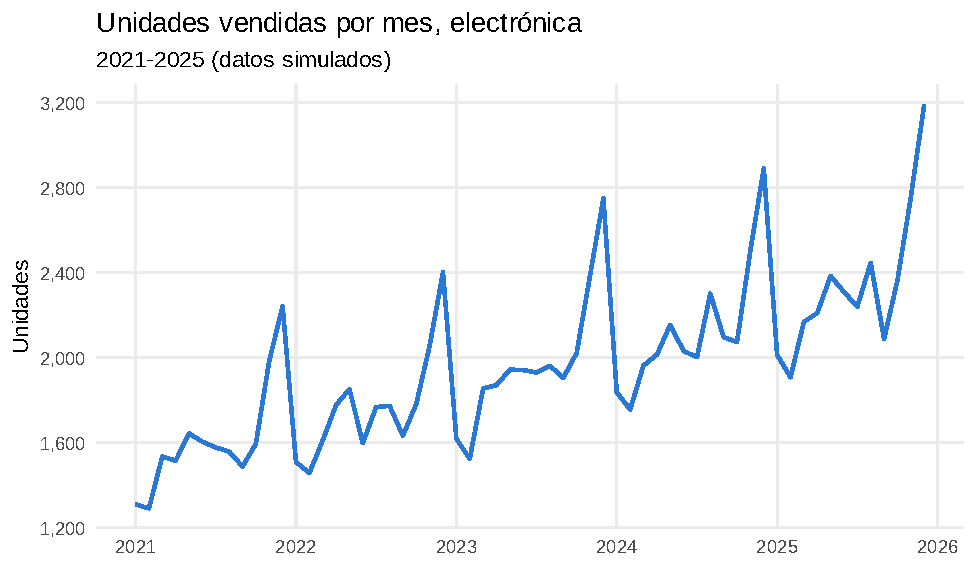
\includegraphics[width=0.9\textwidth]{m07-serie}
\caption{Serie mensual de unidades vendidas: tendencia creciente y picos cada
fin de año.}
\label{fig:m07-serie}
\end{figure}

\codigo{autoplot()} de \paquete{forecast} convierte objetos de series de tiempo
en gráficas de \paquete{ggplot2}, así que puedes agregarles capas, escalas y
temas como a cualquier otra.

\subsection{Descomposición: separar tendencia, estacionalidad y ruido}

\begin{rcode}
descomposicion <- decompose(serie, type = "multiplicative")

# Índices estacionales: cuánto se aleja cada mes de un mes "normal"
nombres_mes <- c("ene", "feb", "mar", "abr", "may", "jun",
                 "jul", "ago", "sep", "oct", "nov", "dic")
tibble(mes = nombres_mes, indice = round(descomposicion$figure, 3)) %>%
  arrange(desc(indice)) %>%
  head(4)

grafico_descomp <- autoplot(descomposicion) +
  labs(title = "Descomposición multiplicativa de la serie",
       x = NULL) +
  theme_minimal() +
  theme(panel.grid.minor = element_blank())
grafico_descomp
\end{rcode}

\begin{rsalida}
# A tibble: 4 x 2
  mes   indice
  <chr>  <dbl>
1 dic     1.32
2 nov     1.16
3 may     1.03
4 ago     1   
\end{rsalida}

\begin{figure}[H]
\centering
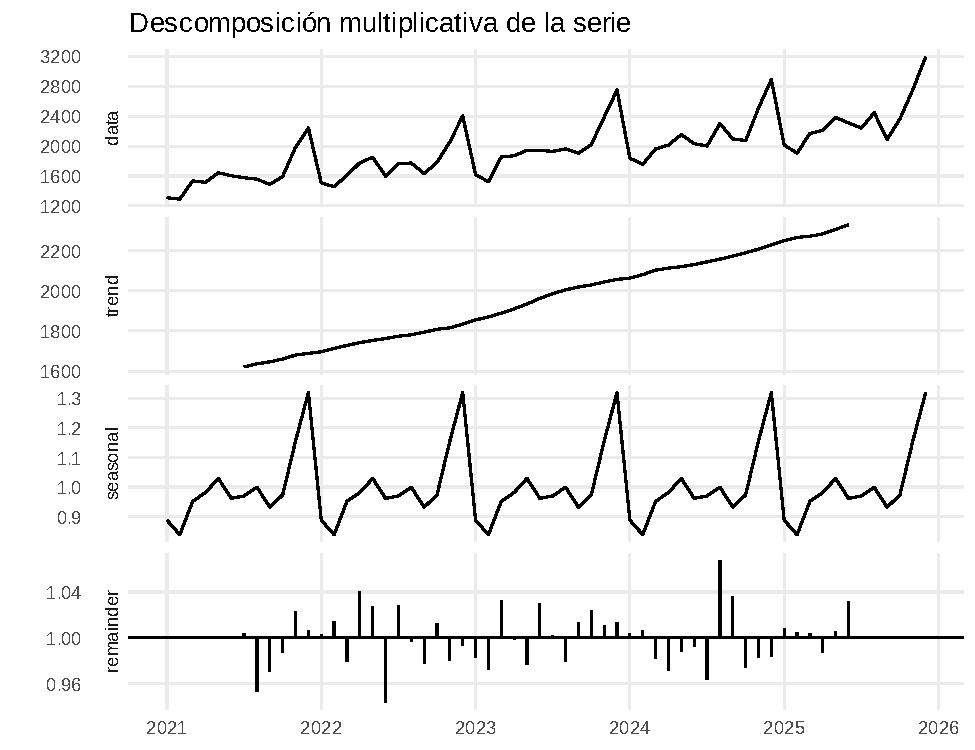
\includegraphics[width=0.9\textwidth]{m07-descomposicion}
\caption{Descomposición de la serie: datos originales, tendencia, componente
estacional y residuo (\emph{remainder}).}
\label{fig:m07-descomposicion}
\end{figure}

Usamos el modelo \emph{multiplicativo} porque la estacionalidad es un
porcentaje (diciembre vende ``32\% más'', no ``400 unidades más''), y ese
porcentaje se mantiene aunque el negocio crezca. Los índices estacionales recuperan
casi exactamente lo que simulamos: diciembre vende 32\% más que un mes normal
(índice 1.32) y noviembre 16\% más (1.16). Esos índices, por sí solos, ya son
información valiosa para planear personal, inventario y presupuesto de
publicidad.

\begin{hazlotu}
Usa \codigo{stl(serie, s.window = "periodic")} en lugar de \codigo{decompose()}
y grafica el resultado con \codigo{autoplot()}. STL es un método de
descomposición más robusto ante valores atípicos (trabaja de forma aditiva;
para una versión multiplicativa aplica \codigo{log()} a la serie).
\end{hazlotu}

\subsection{Entrenamiento y prueba en series de tiempo}

En series de tiempo \textbf{no} se separan los datos al azar: el pasado entrena
y el futuro evalúa. Guardamos los últimos 12 meses (todo 2025) como prueba, que
es exactamente lo que queremos saber hacer: pronosticar un año.

\begin{rcode}
serie_ent    <- window(serie, end = c(2024, 12))   # 2021-2024: 48 meses
serie_prueba <- window(serie, start = c(2025, 1))  # 2025: 12 meses
c(length(serie_ent), length(serie_prueba))
\end{rcode}

\begin{rsalida}
[1] 48 12
\end{rsalida}

\subsection{Cuatro modelos de pronóstico}

\begin{concepto}{Modelos de pronóstico}
\begin{itemize}
  \item \textbf{Ingenuo} (\codigo{naive()}): el próximo mes será igual al
        último. Parece tonto, pero es la línea base obligatoria.
  \item \textbf{Ingenuo estacional} (\codigo{snaive()}): cada mes será igual
        al mismo mes del año anterior (diciembre 2025 = diciembre 2024).
  \item \textbf{ETS} (\codigo{ets()}, \emph{Error, Trend, Seasonal}):
        suavizamiento exponencial; da más peso a los datos recientes y modela
        explícitamente nivel, tendencia y estacionalidad. Elige solo la mejor
        combinación.
  \item \textbf{ARIMA} (\codigo{auto.arima()}): modela la relación de cada mes
        con los meses anteriores y con sus propios errores pasados;
        \codigo{auto.arima()} busca la mejor especificación automáticamente.
\end{itemize}
\end{concepto}

\begin{rcode}
h <- length(serie_prueba)   # horizonte: 12 meses

pron_naive  <- naive(serie_ent, h = h)
pron_snaive <- snaive(serie_ent, h = h)
modelo_ets  <- ets(serie_ent)
pron_ets    <- forecast(modelo_ets, h = h)
modelo_arima <- auto.arima(serie_ent)
pron_arima  <- forecast(modelo_arima, h = h)

modelo_ets     # ¿qué combinación eligió ets()?
modelo_arima
\end{rcode}

\begin{rsalida}
ETS(M,A,M) 

Call:
 ets(y = serie_ent) 

  Smoothing parameters:
    alpha = 0.0199 
    beta  = 4e-04 
    gamma = 1e-04 

  Initial states:
    l = 1527.3166 
    b = 14.5543 
    s = 1.3231 1.1584 0.9739 0.9307 1.0039 0.9739
           0.9589 1.0257 0.9811 0.9589 0.8368 0.8747

  sigma:  0.0339

     AIC     AICc      BIC 
597.8241 618.2241 629.6346 
Series: serie_ent 
ARIMA(0,0,0)(1,1,0)[12] with drift 

Coefficients:
         sar1    drift
      -0.5378  14.9348
s.e.   0.1418   0.7466

sigma^2 = 5463:  log likelihood = -207
AIC=420.01   AICc=420.76   BIC=424.76
\end{rsalida}

\codigo{ets()} eligió un modelo \codigo{ETS(M,A,M)}: error multiplicativo,
tendencia aditiva (\emph{A}, crece una cantidad fija cada mes: \codigo{b =
14.55}, muy cerca de las 15 unidades que simulamos) y estacionalidad
multiplicativa (\emph{M}). \codigo{auto.arima()} eligió un modelo que compara
cada mes con el mismo mes del año anterior (la parte \codigo{(1,1,0)[12]}) más
una deriva (\emph{drift}) de 14.9 unidades por mes: otra forma de describir la
misma tendencia. No necesitas memorizar la notación; lo importante es que
ambos modelos capturaron tendencia y estacionalidad sin que se las
indicáramos.

\subsection{Comparar los modelos con \texorpdfstring{\codigo{accuracy()}}{accuracy()}}

\codigo{accuracy()} calcula las métricas de error del pronóstico contra los
valores reales. Nos interesa la fila \codigo{Test set} (error en 2025, que los
modelos no vieron):

\begin{rcode}
accuracy(pron_ets, serie_prueba)   # salida completa de un modelo

comparacion_ts <- list(Ingenuo = pron_naive,
                       `Ingenuo estacional` = pron_snaive,
                       ETS = pron_ets, ARIMA = pron_arima) %>%
  map_dfr(function(p) {
    acc <- accuracy(p, serie_prueba)["Test set", ]
    tibble(MAE = acc["MAE"], RMSE = acc["RMSE"], MAPE = acc["MAPE"])
  }, .id = "modelo") %>%
  mutate(across(where(is.numeric), ~ round(.x, 1))) %>%
  arrange(MAPE)
comparacion_ts
\end{rcode}

\begin{rsalida}
                    ME     RMSE      MAE        MPE     MAPE
Training set -7.685706 52.06332 43.34896 -0.5184226 2.336622
Test set     27.712908 60.48803 48.44893  1.1527656 2.130479
                  MASE       ACF1 Theil's U
Training set 0.2483390  0.1141467        NA
Test set     0.2775559 -0.5886038 0.2412182
# A tibble: 4 x 4
  modelo               MAE  RMSE  MAPE
  <chr>              <dbl> <dbl> <dbl>
1 ARIMA               46.8  68.3   2  
2 ETS                 48.4  60.5   2.1
3 Ingenuo estacional 205.  219.    8.7
4 Ingenuo            600.  642    27.3
\end{rsalida}

La salida completa de \codigo{accuracy()} incluye más métricas (\codigo{ME}
es el error promedio con signo: 27.7 indica que ETS se quedó ligeramente corto
en 2025; \codigo{MASE} compara contra el ingenuo). En la tabla resumida, ETS y
ARIMA prácticamente empatan con errores de apenas 2\% (MAPE) en 2025: ARIMA
tiene un MAE algo menor (46.8 contra 48.4) y ETS un RMSE menor (60.5 contra
68.3), es decir, menos errores grandes. El ingenuo estacional se equivoca 8.7\%
porque ignora el crecimiento, y el ingenuo simple, 27.3\%, porque ignora la
estacionalidad: diciembre de 2024 no se parece a enero de 2025. Elegimos ETS
por su menor RMSE: en inventario, los errores grandes son los que duelen.

\begin{rcode}
grafico_comparacion <- autoplot(window(serie, start = c(2023, 1)),
                                color = "black", linewidth = 0.6) +
  autolayer(pron_snaive, series = "Ingenuo estacional", PI = FALSE) +
  autolayer(pron_ets, series = "ETS", PI = FALSE) +
  autolayer(pron_arima, series = "ARIMA", PI = FALSE) +
  scale_color_manual(values = paleta_libro[c(2, 1, 3)]) +
  scale_y_continuous(labels = scales::comma) +
  labs(title = "Pronósticos de 2025 contra la realidad",
       subtitle = "Negro: ventas reales; entrenamiento hasta dic-2024",
       x = NULL, y = "Unidades", color = NULL) +
  theme_minimal() +
  theme(panel.grid.minor = element_blank(), legend.position = "top")
grafico_comparacion
\end{rcode}

\begin{figure}[H]
\centering
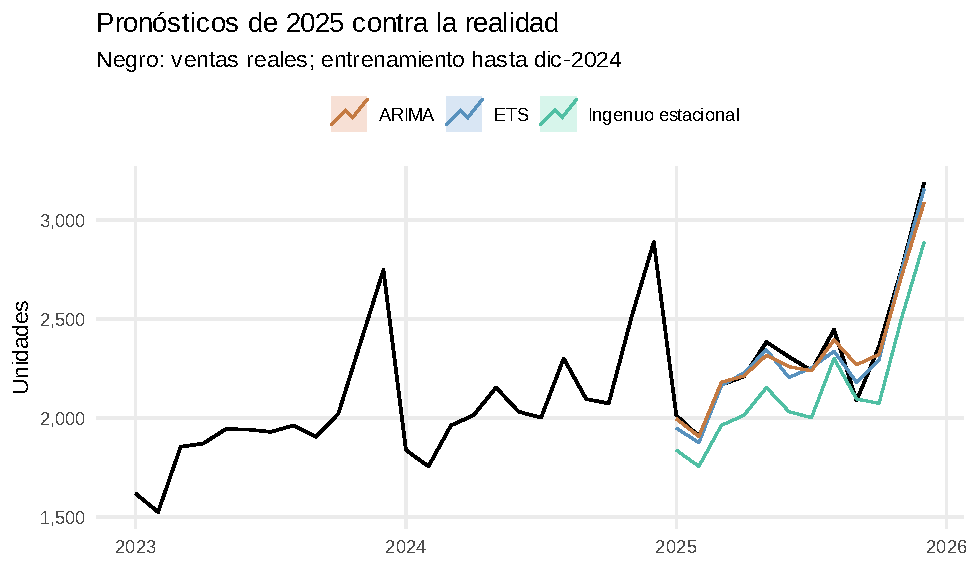
\includegraphics[width=0.9\textwidth]{m07-comparacion-pronosticos}
\caption{Pronósticos de 2025 de tres modelos contra las ventas reales. ETS y
ARIMA siguen de cerca la realidad; el ingenuo estacional se queda corto porque
ignora el crecimiento.}
\label{fig:m07-comparacion-pronosticos}
\end{figure}

\subsection{Pronóstico final con intervalos}

Una vez elegido el modelo, se \textbf{reentrena con todos los datos}
(incluido 2025) para pronosticar 2026:

\begin{rcode}
modelo_final <- ets(serie)
pronostico_2026 <- forecast(modelo_final, h = 12, level = c(80, 95))
pronostico_2026
\end{rcode}

\begin{rsalida}
         Point Forecast    Lo 80    Hi 80    Lo 95    Hi 95
Jan 2026       2125.663 2040.343 2210.984 1995.177 2256.150
Feb 2026       2037.570 1955.751 2119.389 1912.439 2162.702
Mar 2026       2333.729 2239.979 2427.480 2190.350 2477.108
Apr 2026       2400.133 2303.674 2496.591 2252.612 2547.653
May 2026       2547.002 2444.599 2649.406 2390.390 2703.615
Jun 2026       2411.232 2314.247 2508.217 2262.906 2559.557
Jul 2026       2420.791 2323.381 2518.200 2271.816 2569.766
Aug 2026       2548.945 2446.337 2651.553 2392.020 2705.871
Sep 2026       2349.700 2255.074 2444.327 2204.982 2494.419
Oct 2026       2488.212 2387.967 2588.457 2334.901 2641.523
Nov 2026       2975.194 2855.281 3095.107 2791.803 3158.585
Dec 2026       3411.931 3274.360 3549.501 3201.535 3622.327
\end{rsalida}

\begin{concepto}{Intervalos de predicción}
\codigo{Point Forecast} es la estimación central. \codigo{Lo 80} y \codigo{Hi 80}
forman el intervalo del 80\%: esperamos que 8 de cada 10 meses la venta real
caiga dentro de ese rango. El intervalo del 95\% es más ancho porque exige más
seguridad. Los intervalos se ensanchan a medida que el pronóstico se aleja:
es más difícil predecir diciembre que enero.
\end{concepto}

\begin{rcode}
grafico_pronostico <- autoplot(pronostico_2026, color = color_principal,
                               fcol = color_resalte, flwd = 0.8) +
  scale_y_continuous(labels = scales::comma) +
  labs(title = "Pronóstico de unidades para 2026",
       subtitle = "Modelo ETS; bandas de 80 % y 95 %",
       x = NULL, y = "Unidades") +
  theme_minimal() +
  theme(panel.grid.minor = element_blank())
grafico_pronostico
\end{rcode}

\begin{figure}[H]
\centering
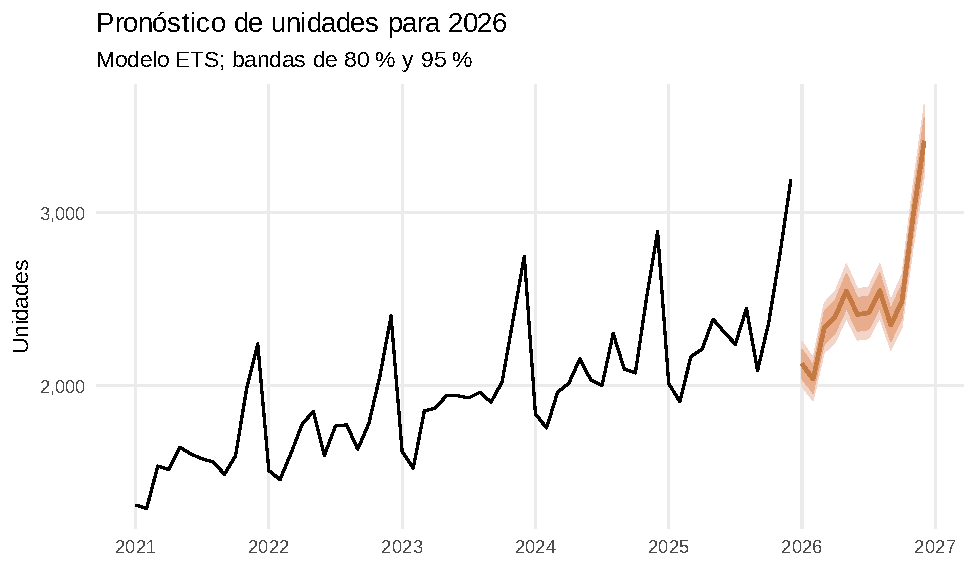
\includegraphics[width=0.9\textwidth]{m07-pronostico}
\caption{Pronóstico de 12 meses con intervalos de predicción del 80\% (banda
oscura) y 95\% (banda clara).}
\label{fig:m07-pronostico}
\end{figure}

\subsection{Comunicar la incertidumbre a la dirección}

Un pronóstico sin rango es una promesa que no se va a cumplir exactamente.
Presenta siempre tres escenarios en lenguaje de negocio:

\begin{rcode}
tabla_direccion <- tibble(
  mes         = format(seq(as.Date("2026-01-01"), by = "month",
                           length.out = 12), "%b %Y"),
  pesimista   = round(pronostico_2026$lower[, "80%"]),
  esperado    = round(pronostico_2026$mean),
  optimista   = round(pronostico_2026$upper[, "80%"])
)
tabla_direccion %>% slice(c(1, 6, 11, 12))
sum(tabla_direccion$esperado)   # unidades esperadas en todo 2026
\end{rcode}

\begin{rsalida}
# A tibble: 4 x 4
  mes      pesimista esperado optimista
  <chr>        <dbl>    <dbl>     <dbl>
1 ene 2026      2040     2126      2211
2 jun 2026      2314     2411      2508
3 nov 2026      2855     2975      3095
4 dic 2026      3274     3412      3550
[1] 30051
\end{rsalida}

Para la dirección: en diciembre de 2026 esperamos vender 3{,}412 unidades; en
un escenario pesimista (límite inferior del 80\%), 3{,}274, y en uno optimista,
3{,}550. En todo el año se esperan 30{,}051 unidades. Observa que
\codigo{format(..., "\%b \%Y")} sí respeta el idioma del sistema (``ene
2026'').

\begin{negocio}{Cómo presentar un pronóstico}
\begin{itemize}
  \item Da un rango y un escenario central: ``esperamos vender 3{,}412 unidades
        en diciembre; con 80\% de confianza, entre 3{,}274 y 3{,}550''.
  \item Explica los supuestos: ``suponemos que el crecimiento y la
        estacionalidad de los últimos cinco años se mantienen''.
  \item Di qué lo podría romper: una devaluación, un competidor nuevo, una
        promoción extraordinaria, una pandemia.
  \item Compara con el pronóstico anterior y con lo que realmente pasó: la
        credibilidad se gana mostrando el historial de aciertos y errores.
\end{itemize}
\end{negocio}

\subsection{Del pronóstico al inventario: stock de seguridad}

El pronóstico central no basta para decidir cuánto pedir: si pides exactamente
lo esperado, la mitad de los meses te faltará mercancía. El
\termino{stock de seguridad} es el inventario extra que cubre la
incertidumbre. Una fórmula sencilla y muy usada es:

\[
\text{stock de seguridad} = z \times \sigma_{\text{error}} \times \sqrt{L}
\]

donde $z$ depende del \termino{nivel de servicio} deseado (1.28 para 90\%,
1.65 para 95\%, 2.33 para 99\%), $\sigma_{\text{error}}$ es la desviación
estándar del error de pronóstico (usaremos el RMSE del modelo ETS en 2025) y
$L$ es el tiempo de reabastecimiento en meses.

\begin{rcode}
nivel_servicio <- 0.95
z <- qnorm(nivel_servicio)                 # 1.645
error_tipico <- comparacion_ts %>%
  filter(modelo == "ETS") %>% pull(RMSE)   # error típico en 2025
tiempo_entrega <- 2                        # meses de anticipación

stock_seguridad <- z * error_tipico * sqrt(tiempo_entrega)

tabla_direccion %>%
  slice(11:12) %>%
  mutate(stock_seguridad = round(stock_seguridad),
         pedido_sugerido = esperado + stock_seguridad) %>%
  select(mes, esperado, stock_seguridad, pedido_sugerido)
\end{rcode}

\begin{rsalida}
# A tibble: 2 x 4
  mes      esperado stock_seguridad pedido_sugerido
  <chr>       <dbl>           <dbl>           <dbl>
1 nov 2026     2975             141            3116
2 dic 2026     3412             141            3553
\end{rsalida}

Con un nivel de servicio de 95\% ($z = 1.645$), un error típico de 60.5
unidades y dos meses de anticipación, el stock de seguridad es de 141
unidades. El pedido sugerido para diciembre es de 3{,}553 unidades: el
pronóstico central más el colchón. Subir el nivel de servicio a 99\% aumenta el
colchón (y el costo de inventario); es otra decisión de negocio que el
modelo te ayuda a cuantificar.

\begin{advertencia}
Un modelo de series de tiempo asume que \textbf{el futuro se parece al
pasado}. No sabe que el próximo año abrirás 20 tiendas, que un proveedor
quebró o que habrá una promoción extraordinaria. Pronostica a 12 meses; más
allá, la incertidumbre crece tanto que el número deja de ser útil para
decisiones operativas. Y revisa el pronóstico cada mes con los datos nuevos.
\end{advertencia}

% ============================================================================
\section{Caso 5: análisis de canasta (market basket)}
\label{sec:m7-canasta}

\begin{ejemplo}{¿Qué le ofrecemos al cliente que compra una laptop?}
Una tienda de electrónica y papelería quiere diseñar promociones de venta
cruzada (\emph{cross-selling}): ``lleva el mouse con 20\% de descuento'',
colocar productos juntos en el anaquel o recomendar productos en la tienda en
línea. La pregunta: \emph{¿qué productos se compran juntos con más frecuencia
de la que esperaríamos por casualidad?}
\end{ejemplo}

El \termino{análisis de canasta} (\emph{market basket analysis}) busca
\termino{reglas de asociación} del tipo \{Laptop\} $\rightarrow$ \{Mouse\}:
``quien compra una laptop tiende a comprar un mouse''. Es aprendizaje no
supervisado: no hay nada que predecir, solo patrones que descubrir en los
tickets de compra.

\subsection{Soporte, confianza y lift}

Tres medidas describen una regla $X \rightarrow Y$:

\begin{itemize}
  \item \termino{Soporte}: proporción de tickets que contienen $X$ \emph{y}
        $Y$. Mide qué tan frecuente es la combinación.
        \[ \text{soporte}(X \rightarrow Y) = \frac{\text{tickets con } X \text{ y } Y}{\text{total de tickets}} \]
  \item \termino{Confianza}: de los tickets que tienen $X$, qué proporción
        también tiene $Y$. Es una probabilidad condicional.
        \[ \text{confianza}(X \rightarrow Y) = \frac{\text{tickets con } X \text{ y } Y}{\text{tickets con } X} \]
  \item \termino{Lift}: cuántas veces más probable es comprar $Y$ cuando se
        compra $X$, comparado con comprar $Y$ en general.
        \[ \text{lift}(X \rightarrow Y) = \frac{\text{confianza}(X \rightarrow Y)}{\text{soporte}(Y)} \]
        Lift $= 1$: no hay relación; lift $> 1$: se compran juntos más de lo
        esperado; lift $< 1$: se ``evitan''.
\end{itemize}

\textbf{Ejemplo a mano.} En 1{,}000 tickets, 100 tienen laptop, 200 tienen
mouse y 60 tienen ambos.

\begin{itemize}
  \item Soporte de \{Laptop, Mouse\}: $60 / 1{,}000 = 0.06$ (6\% de los tickets).
  \item Confianza de Laptop $\rightarrow$ Mouse: $60 / 100 = 0.60$ (60\% de
        quienes compran laptop llevan mouse).
  \item Soporte de Mouse: $200 / 1{,}000 = 0.20$ (20\% de todos los tickets
        llevan mouse).
  \item Lift: $0.60 / 0.20 = 3$. Quien compra laptop tiene \textbf{tres veces}
        más probabilidad de llevar mouse que un cliente cualquiera.
\end{itemize}

\begin{advertencia}
La confianza sola engaña. Si el 30\% de todos los tickets lleva papel, una
regla ``Laptop $\rightarrow$ Papel'' con confianza de 30\% parece buena, pero
su lift es 1: el papel se vende igual con o sin laptop. Por eso ordenamos las
reglas por lift y exigimos un soporte mínimo (las reglas con muy pocos tickets
son casualidades).
\end{advertencia}

\subsection{¿Sirven los datos del curso?}

Antes de simular, revisemos si \archivo{transacciones.csv} permite formar
canastas. Consideremos una canasta como todos los productos que un cliente
compró el mismo día:

\begin{rcode}
canastas_curso <- transacciones %>%
  group_by(cliente_id, fecha) %>%
  summarise(productos = n_distinct(producto_id), .groups = "drop")

canastas_curso %>% count(productos, name = "canastas")
\end{rcode}

\begin{rsalida}
# A tibble: 2 x 2
  productos canastas
      <int>    <int>
1         1      974
2         2       13
\end{rsalida}

De 987 canastas, solo 13 tienen dos productos; ninguna tiene más. Con los datos
del curso no hay canastas que analizar (cada transacción es prácticamente una
compra de un solo producto). Otra vez: sin señal no hay modelo. Simulamos, por
lo tanto, 3{,}000 tickets de una tienda con asociaciones conocidas.

\subsection{Tickets simulados con asociaciones conocidas}

Ocho productos se compran de forma independiente, y cuatro dependen de otro:
el mouse y la funda son mucho más probables si el ticket incluye una laptop, el
cable HDMI si incluye un monitor y la tinta si incluye una impresora.

\begin{rcode}
set.seed(123)
n_tickets <- 3000
tickets_ancho <- tibble(
  ticket_id = 1:n_tickets,
  Laptop    = rbinom(n_tickets, 1, 0.08),   # 1 = el ticket lo incluye
  Monitor   = rbinom(n_tickets, 1, 0.07),
  Impresora = rbinom(n_tickets, 1, 0.05),
  Audifonos = rbinom(n_tickets, 1, 0.15),
  USB       = rbinom(n_tickets, 1, 0.18),
  Papel     = rbinom(n_tickets, 1, 0.20),
  Teclado   = rbinom(n_tickets, 1, 0.08)
) %>%
  mutate(
    # Asociaciones "reales" que el análisis debe descubrir
    Mouse = if_else(Laptop == 1, rbinom(n(), 1, 0.60),
                    rbinom(n(), 1, 0.08)),
    Funda = if_else(Laptop == 1, rbinom(n(), 1, 0.40),
                    rbinom(n(), 1, 0.02)),
    `Cable HDMI` = if_else(Monitor == 1, rbinom(n(), 1, 0.50),
                           rbinom(n(), 1, 0.04)),
    Tinta = if_else(Impresora == 1, rbinom(n(), 1, 0.70),
                    rbinom(n(), 1, 0.06))
  )

# Formato largo: una fila por ticket y producto (como en un sistema real)
tickets <- tickets_ancho %>%
  pivot_longer(-ticket_id, names_to = "producto", values_to = "compro") %>%
  filter(compro == 1) %>%
  select(-compro)

head(tickets, 5)
n_total <- n_distinct(tickets$ticket_id)   # tickets con al menos 1 producto
n_total
\end{rcode}

\begin{rsalida}
# A tibble: 5 x 2
  ticket_id producto 
      <int> <chr>    
1         1 Teclado  
2         2 Monitor  
3         2 Audifonos
4         3 USB      
5         4 USB      
[1] 1975
\end{rsalida}

El formato largo (una fila por ticket y producto) es exactamente como vendrían
los datos de un sistema de punto de venta. Hay 1{,}975 tickets con al menos un
producto (los tickets vacíos de la simulación se descartan).

\subsection{Calcular reglas de pares con \texorpdfstring{\paquete{dplyr}}{dplyr}}

Primero el soporte de cada producto:

\begin{rcode}
soporte_producto <- tickets %>%
  count(producto, name = "tickets_x") %>%
  mutate(soporte_x = tickets_x / n_total) %>%
  arrange(desc(soporte_x))
soporte_producto %>% mutate(soporte_x = round(soporte_x, 3))
\end{rcode}

\begin{rsalida}
# A tibble: 11 x 3
   producto   tickets_x soporte_x
   <chr>          <int>     <dbl>
 1 Papel            596     0.302
 2 USB              557     0.282
 3 Audifonos        442     0.224
 4 Mouse            386     0.195
 5 Tinta            276     0.14 
 6 Laptop           225     0.114
 7 Cable HDMI       215     0.109
 8 Teclado          210     0.106
 9 Monitor          205     0.104
10 Impresora        149     0.075
11 Funda            144     0.073
\end{rsalida}

Ahora el truco: un \termino{self-join} (unir la tabla consigo misma por
\codigo{ticket\_id}) genera todos los pares de productos que aparecen en el
mismo ticket. Luego contamos cuántos tickets tiene cada par y calculamos las
tres medidas:

\begin{rcode}
reglas <- tickets %>%
  inner_join(tickets, by = "ticket_id", suffix = c("_x", "_y"),
             relationship = "many-to-many") %>%
  filter(producto_x != producto_y) %>%          # sin pares consigo mismo
  count(producto_x, producto_y, name = "tickets_xy") %>%
  left_join(soporte_producto, by = c("producto_x" = "producto")) %>%
  left_join(soporte_producto %>%
              select(producto_y = producto, soporte_y = soporte_x),
            by = "producto_y") %>%
  mutate(soporte   = tickets_xy / n_total,
         confianza = tickets_xy / tickets_x,
         lift      = confianza / soporte_y)

mejores_reglas <- reglas %>%
  filter(soporte >= 0.02) %>%                   # soporte mínimo: 2 %
  arrange(desc(lift)) %>%
  transmute(regla = paste(producto_x, "->", producto_y),
            tickets_xy, soporte = round(soporte, 3),
            confianza = round(confianza, 3), lift = round(lift, 2))
mejores_reglas %>% head(10)
\end{rcode}

\begin{rsalida}
# A tibble: 10 x 5
   regla                 tickets_xy soporte confianza  lift
   <chr>                      <int>   <dbl>     <dbl> <dbl>
 1 Funda -> Laptop               82   0.042     0.569  5   
 2 Laptop -> Funda               82   0.042     0.364  5   
 3 Impresora -> Tinta           104   0.053     0.698  4.99
 4 Tinta -> Impresora           104   0.053     0.377  4.99
 5 Cable HDMI -> Monitor        105   0.053     0.488  4.71
 6 Monitor -> Cable HDMI        105   0.053     0.512  4.71
 7 Laptop -> Mouse              136   0.069     0.604  3.09
 8 Mouse -> Laptop              136   0.069     0.352  3.09
 9 Funda -> Mouse                61   0.031     0.424  2.17
10 Mouse -> Funda                61   0.031     0.158  2.17
\end{rsalida}

El análisis descubrió exactamente las cuatro asociaciones que simulamos, y en
ambas direcciones:

\begin{itemize}
  \item \textbf{Impresora $\rightarrow$ Tinta}: confianza de 69.8\% (simulamos
        70\%) y lift de 4.99. Casi 7 de cada 10 compradores de impresora llevan
        tinta.
  \item \textbf{Monitor $\rightarrow$ Cable HDMI}: confianza de 51.2\% (simulamos
        50\%), lift de 4.71.
  \item \textbf{Laptop $\rightarrow$ Mouse}: confianza de 60.4\% (simulamos
        60\%), lift de 3.09, y es la regla con más tickets (136).
  \item \textbf{Laptop $\rightarrow$ Funda}: lift de 5.0, el más alto.
\end{itemize}

Observa que el lift es simétrico (Laptop $\rightarrow$ Funda y Funda
$\rightarrow$ Laptop tienen el mismo), pero la confianza no: 56.9\% de quienes
compran funda llevan laptop, pero solo 36.4\% de quienes compran laptop llevan
funda. Y aparece una regla que \emph{no} simulamos directamente: Funda
$\rightarrow$ Mouse (lift 2.17). No es que la funda ``cause'' el mouse: ambos
se compran con laptop. Las reglas de asociación describen coocurrencias, no
causas.

\begin{rcode}
grafico_lift <- mejores_reglas %>%
  filter(lift > 1.5) %>%
  ggplot(aes(x = lift, y = reorder(regla, lift))) +
  geom_col(fill = color_principal, width = 0.7) +
  geom_vline(xintercept = 1, color = color_gris, linetype = "dashed") +
  labs(title = "Reglas de asociación con mayor lift",
       subtitle = "Soporte mínimo 2 %; la línea punteada es lift = 1",
       x = "Lift (veces más probable que al azar)", y = NULL) +
  theme_minimal() +
  theme(panel.grid.minor = element_blank(),
        panel.grid.major.y = element_blank())
grafico_lift
\end{rcode}

\begin{figure}[H]
\centering
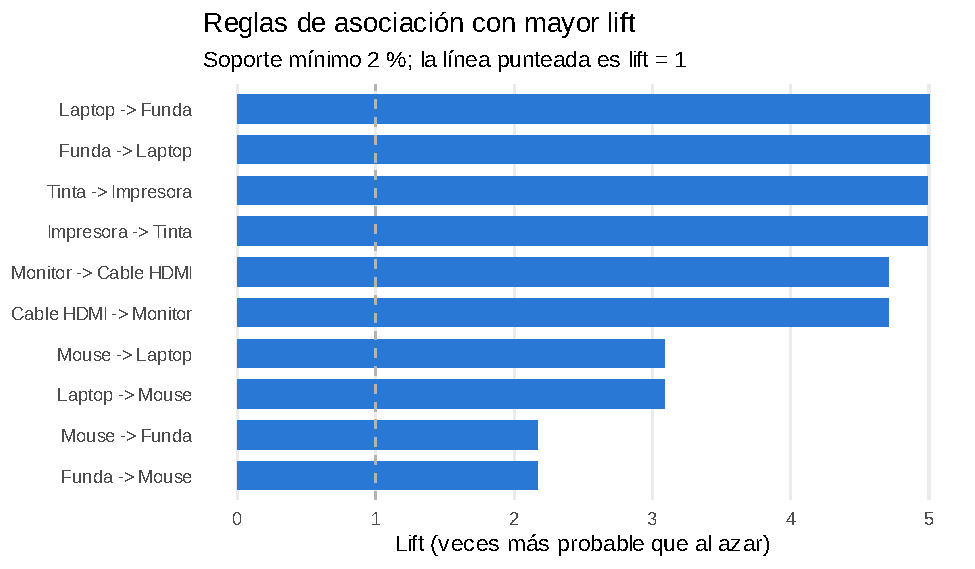
\includegraphics[width=0.9\textwidth]{m07-lift}
\caption{Reglas de asociación ordenadas por lift. Las diez reglas corresponden
a los cuatro pares que simulamos, en ambas direcciones, más la relación
indirecta Funda--Mouse.}
\label{fig:m07-lift}
\end{figure}

¿Y las reglas con lift menor a 1? También dan información:

\begin{rcode}
mejores_reglas %>% arrange(lift) %>% head(3)
\end{rcode}

\begin{rsalida}
# A tibble: 3 x 5
  regla              tickets_xy soporte confianza  lift
  <chr>                   <int>   <dbl>     <dbl> <dbl>
1 Papel -> USB              100   0.051     0.168  0.59
2 USB -> Papel              100   0.051     0.18   0.59
3 Audifonos -> Mouse         52   0.026     0.118  0.6 
\end{rsalida}

Papel y USB aparecen juntos \emph{menos} de lo esperado (lift 0.59), aunque
los simulamos de forma independiente. Es un efecto de cómo se forman los datos:
al quedarnos solo con tickets que tienen al menos un producto, los productos
frecuentes ``compiten'' por aparecer. En datos reales, un lift claramente
menor a 1 suele indicar \textbf{productos sustitutos} (dos marcas de la misma
tinta, por ejemplo): no tiene sentido promocionarlos juntos. La lección es que
ningún número se interpreta sin entender cómo se generaron los datos.

\subsection{Con el paquete arules}

Para canastas con cientos de productos y reglas de más de dos productos
(\{Laptop, Mouse\} $\rightarrow$ \{Funda\}), el estándar en R es el paquete
\paquete{arules}, que implementa el algoritmo \termino{Apriori}. No está
instalado en este entorno, pero así se usaría con los mismos datos:

\begin{rnoejecutar}
install.packages("arules")
library(arules)

# Convertir a formato de transacciones: una lista de productos por ticket
lista_tickets <- split(tickets$producto, tickets$ticket_id)
trans <- as(lista_tickets, "transactions")
summary(trans)

reglas_apriori <- apriori(trans,
                          parameter = list(supp = 0.02, conf = 0.3,
                                           minlen = 2))
inspect(head(sort(reglas_apriori, by = "lift"), 10))
\end{rnoejecutar}

\subsection{De las reglas a las recomendaciones}

\begin{negocio}{Acciones de venta cruzada}
\begin{itemize}
  \item \textbf{Paquetes}: ``Kit oficina en casa'' con Impresora + Tinta, o
        ``Kit estudiante'' con Laptop + Mouse + Funda, con un pequeño descuento
        sobre la suma.
  \item \textbf{Ubicación en tienda}: los cables HDMI junto a los monitores;
        las tintas a la vista desde el pasillo de impresoras.
  \item \textbf{Recomendaciones en línea}: al agregar una laptop al carrito,
        mostrar mouse y funda (las reglas con mayor confianza desde Laptop).
  \item \textbf{No descontar lo que ya se vende junto}: si el 70\% de quienes
        compran impresora ya lleva tinta, un descuento en tinta regala
        margen. Mejor ofrecer el descuento al 30\% restante (por ejemplo, en
        el correo de seguimiento).
  \item \textbf{Medir}: lanza la promoción en algunas tiendas y compara con
        otras similares sin promoción antes de extenderla.
\end{itemize}
\end{negocio}

\begin{hazlotu}
Calcula las reglas cuyo antecedente es \codigo{"Laptop"}
(\codigo{filter(producto\_x == "Laptop")}) y ordénalas por confianza. ¿Qué
producto recomendarías primero en el carrito de compras? ¿Coincide con el orden
por lift?
\end{hazlotu}

% ============================================================================
\section{Llevar el modelo a producción}
\label{sec:m7-produccion}

Un modelo que vive solo en tu computadora no genera valor. \termino{Desplegar}
(o ``poner en producción'') un modelo significa que se ejecuta de forma
periódica y confiable sobre datos nuevos, y que sus resultados llegan a quien
toma decisiones. En BI, lo más común es empezar con algo sencillo: un script
que cada lunes puntúa a los clientes y deja un CSV (o una tabla en la base de
datos, Módulo~\ref{cap:bases-datos}) que alimenta el tablero y el call center.

\subsection{Guardar y cargar el modelo}

No necesitas reentrenar cada vez: guarda el objeto del modelo en un archivo
\archivo{.rds} con \codigo{saveRDS()} y cárgalo con \codigo{readRDS()}.

\begin{rcode}
dir.create("resultados", showWarnings = FALSE)

saveRDS(modelo_log, "resultados/modelo_churn.rds")

# ... días después, en otro script o en otra computadora:
modelo_cargado <- readRDS("resultados/modelo_churn.rds")

# Comprobamos que predice exactamente lo mismo
all.equal(predict(modelo_cargado, churn_prueba, type = "response"),
          predict(modelo_log, churn_prueba, type = "response"))
\end{rcode}

\begin{rsalida}
[1] TRUE
\end{rsalida}

\begin{consejo}
Guarda junto al modelo la información para reproducirlo: fecha de
entrenamiento, periodo de datos, métricas en prueba y versión de R y de los
paquetes. Un nombre como \archivo{modelo\_churn\_2025-06\_v2.rds} y una nota
en un archivo de texto te ahorrarán muchos dolores de cabeza.
\end{consejo}

\subsection{Una función para puntuar clientes nuevos}

Encapsula la predicción en una función que \textbf{valide} los datos de
entrada, calcule la probabilidad y la traduzca a una acción:

\begin{rcode}
predecir_churn <- function(nuevos_datos, modelo, umbral = 0.15) {
  # 1. Validar que vengan todas las columnas que el modelo necesita
  necesarias <- c("antiguedad_meses", "plan", "uso_mensual", "quejas_6m",
                  "pagos_tardios", "genero", "edad")
  faltan <- setdiff(necesarias, names(nuevos_datos))
  if (length(faltan) > 0) {
    stop("Faltan columnas: ", paste(faltan, collapse = ", "))
  }
  # 2. Mismos niveles de factor que en el entrenamiento
  nuevos_datos <- nuevos_datos %>%
    mutate(plan = factor(plan, levels = c("Básico", "Estándar",
                                          "Premium")))
  # 3. Probabilidad y acción sugerida
  nuevos_datos %>%
    mutate(
      prob_churn = predict(modelo, newdata = nuevos_datos,
                           type = "response"),
      nivel_riesgo = cut(prob_churn, breaks = c(0, umbral, 0.5, 1),
                         labels = c("Bajo", "Medio", "Alto"),
                         include.lowest = TRUE),
      accion = if_else(prob_churn >= umbral, "Llamar", "Sin acción")
    )
}
\end{rcode}

Simulamos un lote de 500 clientes activos de esta semana (en la vida real
vendría de la base de datos) y lo puntuamos:

\begin{rcode}
set.seed(123)
lote_semana <- tibble(
  cliente_id       = sprintf("N%04d", 1:500),
  antiguedad_meses = sample(1:72, 500, replace = TRUE),
  plan             = sample(c("Básico", "Estándar", "Premium"), 500,
                            replace = TRUE, prob = c(0.5, 0.3, 0.2)),
  uso_mensual      = rpois(500, 8),
  quejas_6m        = rpois(500, 0.8),
  pagos_tardios    = rpois(500, 0.4),
  genero           = sample(c("F", "M"), 500, replace = TRUE),
  edad             = sample(18:70, 500, replace = TRUE)
)

puntuados <- predecir_churn(lote_semana, modelo_cargado)
puntuados %>% count(nivel_riesgo, accion)

# Exportar la lista para el equipo de retención
puntuados %>%
  filter(accion == "Llamar") %>%
  arrange(desc(prob_churn)) %>%
  mutate(prob_churn = round(prob_churn, 3)) %>%
  select(cliente_id, plan, quejas_6m, prob_churn, nivel_riesgo) %>%
  write_csv("resultados/clientes_a_llamar.csv")

file.exists("resultados/clientes_a_llamar.csv")
\end{rcode}

\begin{rsalida}
# A tibble: 3 x 3
  nivel_riesgo accion         n
  <fct>        <chr>      <int>
1 Bajo         Sin acción   275
2 Medio        Llamar       142
3 Alto         Llamar        83
[1] TRUE
\end{rsalida}

De los 500 clientes, 225 superan el umbral de 0.15 y se llaman: 83 de riesgo
alto (probabilidad de 0.5 o más) y 142 de riesgo medio; 275 no requieren
acción. \codigo{file.exists()} confirma que el archivo quedó en
\archivo{resultados/}. Si el equipo solo puede hacer 150 llamadas, empieza por
los de riesgo alto y sigue en orden de probabilidad (o de pérdida esperada).

¿Qué pasa si alguien le pasa a la función un archivo incompleto? En lugar de un
error críptico de R, recibe un mensaje claro:

\begin{rnoejecutar}
predecir_churn(select(lote_semana, -quejas_6m), modelo_cargado)
#> Error in predecir_churn(select(lote_semana, -quejas_6m), modelo_cargado):
#>   Faltan columnas: quejas_6m
\end{rnoejecutar}

\subsection{Monitoreo y reentrenamiento}

Los modelos se degradan con el tiempo porque el mundo cambia. Se llama
\termino{deriva de datos} (\emph{data drift}) a cuando los datos nuevos ya no
se parecen a los de entrenamiento (por ejemplo, llega una ola de clientes
nuevos por una campaña) y \termino{deriva de concepto} (\emph{concept drift})
a cuando cambia la relación entre variables y respuesta (un competidor lanza
un plan más barato y ahora se van también los clientes antiguos).

Un monitoreo básico compara cada semana las variables del lote con las del
entrenamiento:

\begin{rcode}
comparar_distribucion <- function(entrenamiento, nuevo, variables) {
  map_dfr(variables, function(v) {
    tibble(variable = v,
           media_entrenamiento = mean(entrenamiento[[v]]),
           media_nuevo = mean(nuevo[[v]]))
  }) %>%
    mutate(cambio_pct = round(100 * (media_nuevo - media_entrenamiento) /
                                media_entrenamiento, 1),
           alerta = if_else(abs(cambio_pct) > 20, "REVISAR", "ok"))
}

comparar_distribucion(churn_ent, lote_semana,
                      c("antiguedad_meses", "uso_mensual", "quejas_6m",
                        "pagos_tardios")) %>%
  mutate(across(starts_with("media"), ~ round(.x, 2)))
\end{rcode}

\begin{rsalida}
# A tibble: 4 x 5
  variable         media_entrenamiento media_nuevo cambio_pct alerta
  <chr>                          <dbl>       <dbl>      <dbl> <chr> 
1 antiguedad_meses               36.7        36.8         0.3 ok    
2 uso_mensual                     7.97        8.22        3.2 ok    
3 quejas_6m                       0.78        0.79        2.4 ok    
4 pagos_tardios                   0.41        0.39       -4   ok    
\end{rsalida}

En este lote todas las variables se parecen a las del entrenamiento (cambios
de 4\% o menos), así que no hay alerta. Si un mes la media de quejas saltara
de 0.78 a 1.5 (por ejemplo, por una falla en el servicio), el modelo seguiría
funcionando, pero la tasa de ``Llamar'' se dispararía y convendría revisar
tanto el modelo como la operación. El umbral de 20\% es arbitrario: ajústalo a
tu negocio. Existen medidas más formales, como el índice de estabilidad
poblacional (PSI), pero la idea es la misma.

Buenas prácticas de monitoreo y reentrenamiento:

\begin{itemize}
  \item \textbf{Mide el desempeño real}: tres meses después, compara las
        predicciones con quién realmente se fue. Si el AUC cae de 0.86 a 0.70,
        es hora de reentrenar.
  \item \textbf{Reentrena con calendario} (por ejemplo, cada trimestre) y
        \textbf{por alerta} (cuando el monitoreo detecta cambios).
  \item \textbf{Compara el modelo nuevo contra el actual} en los mismos datos
        de prueba antes de reemplazarlo.
  \item \textbf{Automatiza}: programa el script con el Programador de tareas
        de Windows, \codigo{cron} o RStudio Connect, y envía un reporte
        automático (Módulo~\ref{cap:reportes}).
\end{itemize}

\subsection{Ética, sesgos y explicabilidad}

Un modelo toma decisiones que afectan a personas: a quién se le ofrece un
descuento, a quién se le aprueba un crédito, a quién se contrata. Tienes la
responsabilidad de que sea justo y explicable.

\begin{itemize}
  \item \textbf{Variables sensibles}: género, edad, estado civil, origen o
        código postal (que puede reflejar nivel socioeconómico) pueden llevar
        a discriminar. En nuestro modelo, género y edad no aportaban nada
        (odds ratios de 1.02 y 0.997, importancia mínima): lo correcto es
        \textbf{quitarlas}. En decisiones como crédito o contratación, su uso
        puede ser además ilegal.
  \item \textbf{Variables ``proxy''}: aunque quites el género, otra variable
        muy correlacionada (por ejemplo, la categoría de productos que compra)
        puede reintroducirlo. Revisa las tasas de predicción por grupo.
  \item \textbf{Sesgo histórico}: si en el pasado solo se ofrecían créditos a
        cierto perfil, el modelo aprenderá que ``solo ese perfil paga bien''.
        El modelo repite los sesgos de los datos.
  \item \textbf{Explicabilidad}: prefiere modelos interpretables (logística,
        árboles) cuando la decisión debe justificarse ante un cliente o un
        regulador. Con modelos de caja negra, usa la importancia de variables
        y explica los casos individuales.
  \item \textbf{Privacidad}: usa solo los datos necesarios, respeta los avisos
        de privacidad y la legislación de protección de datos personales.
\end{itemize}

Revisemos si el modelo trata distinto a hombres y mujeres del lote:

\begin{rcode}
puntuados %>%
  group_by(genero) %>%
  summarise(clientes = n(),
            prob_media = round(mean(prob_churn), 3),
            pct_llamar = round(100 * mean(accion == "Llamar"), 1),
            .groups = "drop")
\end{rcode}

\begin{rsalida}
# A tibble: 2 x 4
  genero clientes prob_media pct_llamar
  <chr>     <int>      <dbl>      <dbl>
1 F           258      0.223       40.7
2 M           242      0.238       49.6
\end{rsalida}

La probabilidad media es casi igual (0.223 contra 0.238), pero se llamaría a
49.6\% de los hombres y a 40.7\% de las mujeres. Como el coeficiente de género
es prácticamente nulo, la diferencia viene de las otras variables de este lote
en particular (por azar, los hombres tienen algo más de quejas o menos uso) y
del efecto pequeño pero no nulo que el modelo le asignó a
\codigo{generoM}. Aun así, este tipo de tabla es la que debes revisar y
documentar: si la diferencia fuera grande y se debiera a la variable
sensible, habría que quitarla y volver a evaluar.

\begin{hazlotu}
Reentrena la regresión logística sin \codigo{genero} ni \codigo{edad} y
calcula su AUC en \codigo{churn\_prueba}. ¿Perdiste capacidad predictiva? Si la
respuesta es ``casi nada'', ya tienes un argumento para usar el modelo más
justo y más simple.
\end{hazlotu}

% ============================================================================
\section{Errores comunes}
\label{sec:m7-errores}

\subsection{Fuga de datos: el modelo demasiado bueno}

Agreguemos a los clientes de churn una variable que el área de atención
registra: si el cliente llamó al área de cancelaciones. Como la mayoría de los
que se van llaman para cancelar, parece una variable maravillosa\ldots

\begin{rcode}
set.seed(123)
churn_fuga <- clientes_churn %>%
  mutate(llamo_cancelaciones = if_else(
    churn == "Si", rbinom(n(), 1, 0.85),   # casi todos los que se van
    rbinom(n(), 1, 0.03)))                 # muy pocos de los que se quedan

fuga_ent    <- churn_fuga[filas_ent, ]    # misma división que antes
fuga_prueba <- churn_fuga[-filas_ent, ]

modelo_fuga <- glm(update(formula_churn, . ~ . + llamo_cancelaciones),
                   data = fuga_ent, family = binomial)
prob_fuga <- predict(modelo_fuga, fuga_prueba, type = "response")
round(calcular_auc(prob_fuga, fuga_prueba$churn), 3)
\end{rcode}

\begin{rsalida}
[1] 0.964
\end{rsalida}

El AUC salta de 0.86 a 0.964. En el laboratorio parece un modelo
extraordinario. Pero en la operación no sirve: cuando sabemos que el cliente
llamó a cancelaciones, ya decidió irse. La variable es una consecuencia del
abandono, no una señal anticipada.

\begin{advertencia}
Pregunta obligatoria para cada variable: \textbf{¿conoceré este dato en el
momento en que tenga que predecir?} Si un modelo tiene resultados
``demasiado buenos para ser verdad'' (AUC mayor a 0.95 en un problema de
comportamiento humano), sospecha primero de fuga de datos.
\end{advertencia}

\subsection{Evaluar con los datos de entrenamiento}

Evaluar un modelo con los mismos datos con que se entrenó da resultados
optimistas, sobre todo en modelos flexibles. El random forest es un caso
extremo:

\begin{rcode}
prob_rf_ent <- predict(modelo_rf, newdata = churn_ent,
                       type = "prob")[, "Si"]
c(auc_entrenamiento = calcular_auc(prob_rf_ent, churn_ent$churn),
  auc_prueba = calcular_auc(churn_prueba$prob_rf, churn_prueba$churn)) %>%
  round(3)
\end{rcode}

\begin{rsalida}
auc_entrenamiento        auc_prueba 
            1.000             0.846 
\end{rsalida}

En entrenamiento, el bosque tiene un AUC perfecto (1.000): cada árbol crece
hasta memorizar a sus clientes. En prueba baja a 0.846. Si hubieras reportado
el 1.000, habrías prometido algo imposible. Por eso existen el conjunto de
prueba, la validación cruzada y el error OOB.

\subsection{Clases desbalanceadas y la exactitud engañosa}

Un banco revisa 2{,}000 transacciones con tarjeta, de las cuales 5\% son
fraude. Un ``modelo'' que dice \emph{siempre} ``no es fraude'':

\begin{rcode}
set.seed(123)
fraude <- tibble(
  es_fraude = factor(if_else(runif(2000) < 0.05, "Si", "No"),
                     levels = c("No", "Si"))
)
prediccion_perezosa <- factor(rep("No", 2000), levels = c("No", "Si"))

metricas_clasificacion(prediccion_perezosa, fraude$es_fraude) %>%
  mutate(across(everything(), ~ round(.x, 3)))
\end{rcode}

\begin{rsalida}
# A tibble: 1 x 5
  exactitud precision sensibilidad especificidad    F1
      <dbl>     <dbl>        <dbl>         <dbl> <dbl>
1     0.947       NaN            0             1   NaN
\end{rsalida}

¡94.7\% de exactitud sin detectar un solo fraude! La sensibilidad es 0 y la
precisión y F1 son \codigo{NaN} (\emph{Not a Number}: división entre cero,
porque el modelo nunca predijo ``Si''). Un modelo inútil con una exactitud
altísima: por eso, con clases desbalanceadas, la exactitud es la métrica menos
informativa.

Qué hacer con clases desbalanceadas:

\begin{itemize}
  \item Reporta sensibilidad, precisión, F1 y AUC, no solo exactitud.
  \item Compara siempre con la línea base ``predecir la clase mayoritaria''.
  \item Ajusta el umbral según costos (sección~\ref{sec:m7-umbral}).
  \item Usa divisiones estratificadas (\codigo{createDataPartition()}).
  \item Si hace falta, rebalancea el entrenamiento: \paquete{caret} lo permite
        con \codigo{trainControl(sampling = "down")} o \codigo{"up"}.
\end{itemize}

\subsection{No escalar antes de k-means}

\begin{rcode}
set.seed(123)
kmeans_sin_escalar <- kmeans(rfm %>% select(recencia, frecuencia, monto),
                             centers = 4, nstart = 25)

rfm %>%
  mutate(grupo = kmeans_sin_escalar$cluster) %>%
  group_by(grupo) %>%
  summarise(clientes = n(), recencia = round(mean(recencia)),
            frecuencia = round(mean(frecuencia), 1),
            monto = round(mean(monto)), .groups = "drop") %>%
  arrange(monto)
\end{rcode}

\begin{rsalida}
# A tibble: 4 x 5
  grupo clientes recencia frecuencia monto
  <int>    <int>    <dbl>      <dbl> <dbl>
1     3       56      106        2.9  1946
2     4       83       66        5    4491
3     1       44       39        6.2  7089
4     2       15       37        9.7 11092
\end{rsalida}

Sin escalar, los grupos quedan ordenados casi perfectamente por monto (de
\$1{,}946 a \$11{,}092): el monto, que se mide en miles, domina la distancia.
La recencia apenas participa: ya no aparece un grupo de Dormidos con 195 días
de recencia como en la segmentación escalada, y los clientes que dejaron de
comprar quedan mezclados con los demás según lo que gastaron. Escalar no es un
detalle técnico: cambia los segmentos y, por lo tanto, las estrategias.

\subsection{Otros errores frecuentes}

\begin{table}[H]
\centering
\small
\caption{Otros errores comunes en proyectos de machine learning.}
\label{tab:m7-errores}
\begin{tabularx}{\textwidth}{>{\raggedright\arraybackslash}p{4cm}
                              >{\raggedright\arraybackslash}X}
\toprule
\textbf{Error} & \textbf{Cómo evitarlo} \\
\midrule
Usar un código como número (\codigo{tienda\_id}, código postal) &
  \codigo{lm(ventas \textasciitilde{} tienda\_id)} estima un solo coeficiente, como si la
  tienda 10 fuera ``diez veces'' la tienda 1. Conviértelo con
  \codigo{factor(tienda\_id)}, como hicimos en la sección~\ref{sec:m7-sin-senal}. \\
Niveles de factor distintos entre entrenamiento y datos nuevos &
  Fija los niveles con \codigo{factor(x, levels = ...)} (como en
  \codigo{predecir\_churn()}). Un nivel nuevo (un plan ``Familiar'')
  produce el error \codigo{factor plan has new levels Familiar}. \\
Extrapolar &
  Un modelo entrenado con tiendas de 150 a 1{,}200 m² no sabe nada de una de
  5{,}000 m². Un pronóstico a 5 años con 5 años de historia es una apuesta,
  no una predicción. \\
Separar series de tiempo al azar &
  El conjunto de prueba siempre son los periodos más recientes
  (\codigo{window()}). \\
Olvidar \codigo{set.seed()} &
  Sin semilla, k-means, la división de datos y el random forest dan
  resultados distintos cada vez y nadie puede reproducir tu análisis. \\
Confundir correlación con causalidad &
  Un coeficiente dice ``se asocia con'', no ``provoca''. Para medir el
  efecto de una acción, diseña un experimento (grupo de control). \\
Nombrar clusters por número &
  Asigna nombres a partir del perfil calculado (sección~\ref{sec:m7-segmentacion}). \\
\bottomrule
\end{tabularx}
\end{table}

% ============================================================================
\section{Resumen del módulo}

\begin{resumen}
\begin{itemize}
  \item El machine learning aprende patrones de datos históricos. Supervisado:
        regresión (números) y clasificación (categorías). No supervisado:
        clustering y reglas de asociación. Las series de tiempo pronostican
        con la historia de la propia variable.
  \item Sin señal no hay modelo: primero verifica que exista relación
        (exploración, línea base).
  \item Evalúa siempre en datos que el modelo no vio (prueba, validación
        cruzada); vigila el sobreajuste y la fuga de datos.
  \item Segmentación: RFM + escalar + k-means (codo, silueta, \codigo{nstart})
        + perfil + nombres basados en el perfil + estrategia por segmento.
        Alternativa sencilla: quintiles con \codigo{ntile()}.
  \item Regresión: \codigo{lm()} explica y predice; mide con MAE, RMSE, MAPE y
        R²; compara con una línea base y con random forest.
  \item Clasificación: logística (odds ratios), árbol (reglas), random forest
        (importancia); matriz de confusión, sensibilidad, precisión, AUC; el
        umbral se elige con costos de negocio.
  \item Series de tiempo: \codigo{ts()}, descomposición, prueba con los
        últimos meses, \codigo{naive}/\codigo{snaive} como línea base,
        \codigo{ets()} y \codigo{auto.arima()}; comunica rangos y calcula
        stock de seguridad.
  \item Canasta: soporte, confianza y lift con un self-join; ordena por lift
        con soporte mínimo.
  \item Producción: \codigo{saveRDS()}, función de puntuación con validación,
        exportar resultados, monitorear deriva, reentrenar y cuidar la ética.
\end{itemize}
\end{resumen}

\begin{table}[H]
\centering
\small
\caption{Guía rápida: del problema a la función de R y la métrica.}
\label{tab:m7-resumen}
\begin{tabularx}{\textwidth}{>{\raggedright\arraybackslash}p{3.2cm}
                              >{\raggedright\arraybackslash}p{2.9cm}
                              >{\raggedright\arraybackslash}p{3.9cm}
                              >{\raggedright\arraybackslash}X}
\toprule
\textbf{Problema} & \textbf{Algoritmo} & \textbf{Función de R} & \textbf{Métrica} \\
\midrule
Segmentar clientes & k-means & \codigo{scale()}, \codigo{kmeans()},
  \codigo{fviz\_nbclust()} & Codo (WSS), silueta \\
Segmentar con reglas & Quintiles RFM & \codigo{ntile()}, \codigo{case\_when()} &
  Tamaño y valor de segmentos \\
Predecir un número & Regresión lineal & \codigo{lm()}, \codigo{predict()} &
  MAE, RMSE, MAPE, R² \\
Predecir un número (no lineal) & Random forest & \codigo{randomForest()} &
  MAE, RMSE, OOB \\
Predecir una categoría & Regresión logística & \codigo{glm(family = binomial)} &
  AUC, sensibilidad, precisión, F1 \\
Reglas explicables & Árbol de decisión & \codigo{rpart()} &
  AUC, matriz de confusión \\
Comparar modelos & Validación cruzada & \codigo{trainControl()},
  \codigo{train()}, \codigo{resamples()} & ROC (AUC) promedio \\
Pronosticar demanda & Ingenuo, ETS, ARIMA & \codigo{snaive()}, \codigo{ets()},
  \codigo{auto.arima()}, \codigo{forecast()} & \codigo{accuracy()}: MAE,
  RMSE, MAPE \\
Productos que se compran juntos & Reglas de asociación & self-join con
  \codigo{inner\_join()}; \codigo{arules::apriori()} & Soporte, confianza,
  lift \\
Usar el modelo & Despliegue & \codigo{saveRDS()}, \codigo{readRDS()},
  \codigo{write\_csv()} & Desempeño real y deriva \\
\bottomrule
\end{tabularx}
\end{table}

% ============================================================================
\section{Ejercicios}
\label{sec:m7-ejercicios}

Para los ejercicios con datos simulados, copia el código de simulación de la
sección correspondiente (con la misma semilla) al inicio de tu script. Todos
los ejercicios suponen que tienes cargados los paquetes de este módulo.

\begin{ejercicio}{m7-1}{Supervisado o no supervisado}
\nivel{Básico}
Para cada situación, indica si es un problema de regresión, clasificación,
clustering, reglas de asociación o series de tiempo, y propón un algoritmo:
(a) estimar el ticket promedio de un cliente nuevo; (b) detectar si un correo
de cliente es una queja; (c) agrupar las sucursales por su mezcla de ventas;
(d) predecir la demanda semanal de pan de muerto; (e) decidir qué producto
recomendar a quien compra una cafetera. Después, con
\archivo{ventas\_retail.csv}, ajusta \codigo{lm(total \textasciitilde{} descuento\_pct + dia\_semana)}
y reporta su R² ajustado. ¿Hay señal?
\end{ejercicio}

\begin{ejercicio}{m7-2}{Métricas de regresión a mano}
\nivel{Básico}
Un gerente pronosticó las ventas (miles de pesos) de 6 sucursales:
reales \codigo{c(120, 95, 150, 80, 110, 130)} y pronosticadas
\codigo{c(110, 100, 140, 90, 115, 120)}. Calcula MAE, RMSE, MAPE y R²
escribiendo las fórmulas en R (sin paquetes). ¿Cuál es el error promedio en
pesos y en porcentaje?
\end{ejercicio}

\begin{ejercicio}{m7-3}{Matriz de confusión e interpretación}
\nivel{Básico}
Un modelo de fraude se evaluó con 1{,}000 transacciones: detectó 40 de los 50
fraudes reales y marcó como fraude 60 transacciones legítimas. Construye la
matriz de confusión como un \codigo{matrix()} de R y calcula exactitud,
precisión, sensibilidad, especificidad y F1. Si cada fraude no detectado
cuesta \$5{,}000 y cada revisión innecesaria \$100, ¿cuál es el costo de los
errores?
\end{ejercicio}

\begin{ejercicio}{m7-4}{Segmentación RFM por reglas}
\nivel{Intermedio}
Con \archivo{transacciones.csv} calcula el RFM de cada cliente (fecha de
corte 2024-01-01) y asigna calificaciones de 1 a 5 con \codigo{ntile()}.
Calcula un puntaje total \codigo{r + f + m} y clasifica en ``Oro'' (13 a 15),
``Plata'' (9 a 12) y ``Bronce'' (3 a 8). Reporta, por nivel, número de
clientes, monto promedio y porcentaje de los ingresos totales.
\end{ejercicio}

\begin{ejercicio}{m7-5}{k-means con otras variables}
\nivel{Intermedio}
Con \archivo{transacciones.csv}, construye por cliente: monto total, ticket
promedio (\codigo{mean(total\_transaccion)}), número de tiendas distintas y
número de productos distintos. Escala las cuatro variables, elige $k$ con la
silueta (entre 2 y 6), entrena k-means con \codigo{nstart = 25} y nombra los
grupos a partir de su perfil (sin escribir números de cluster a mano).
\end{ejercicio}

\begin{ejercicio}{m7-6}{Mejorar el modelo de churn con una variable nueva}
\nivel{Intermedio}
Con los datos simulados de churn (misma semilla y misma división de la
sección~\ref{sec:m7-churn}), crea la variable
\codigo{cliente\_nuevo = antiguedad\_meses <= 6}, agrégala a la regresión
logística y compara el AUC en prueba con el del modelo original. Interpreta la
razón de momios de la nueva variable. Quita también \codigo{genero} y
\codigo{edad}: ¿cambia el AUC?
\end{ejercicio}

\begin{ejercicio}{m7-7}{Umbral con otros costos}
\nivel{Intermedio}
Con las probabilidades de la regresión logística en \codigo{churn\_prueba},
encuentra el umbral que minimiza el costo total si el descuento cuesta \$800
(en lugar de \$300), un cliente perdido cuesta \$3{,}000 y la mitad de los
clientes contactados que iban a irse se retiene. ¿Cuántos clientes se
llamarían? Compara con el umbral óptimo del texto (0.15) y explica la
diferencia.
\end{ejercicio}

\begin{ejercicio}{m7-8}{Pronóstico trimestral}
\nivel{Avanzado}
A partir de la serie mensual simulada de la sección~\ref{sec:m7-series},
construye una serie \emph{trimestral} (suma de cada trimestre, frecuencia 4).
Deja como prueba los 4 trimestres de 2025, compara \codigo{snaive()},
\codigo{ets()} y \codigo{auto.arima()} con \codigo{accuracy()} y pronostica
los 4 trimestres de 2026 con el mejor modelo, reentrenado con toda la serie.
\end{ejercicio}

\begin{ejercicio}{m7-9}{Canasta con reglas de tres productos}
\nivel{Avanzado}
Con los tickets simulados de la sección~\ref{sec:m7-canasta}, calcula el
soporte, la confianza y el lift de la regla \{Laptop, Mouse\} $\rightarrow$
\{Funda\} usando \paquete{dplyr}. Compárala con Laptop $\rightarrow$ Funda.
¿Saber que el cliente ya lleva mouse cambia la probabilidad de que lleve funda?
\end{ejercicio}

\begin{ejercicio}{m7-10}{Reto: sistema de puntuación de churn completo}
\nivel{Reto}
Simula (con \codigo{set.seed(2024)}) 3{,}000 clientes con las mismas variables
y reglas de la sección~\ref{sec:m7-churn}. Entrena con \paquete{caret} una
regresión logística y un random forest (validación cruzada de 5 pliegues, AUC
como métrica), elige el mejor según el AUC en un 30\% de prueba, guárdalo con
\codigo{saveRDS()}, escribe una función \codigo{puntuar()} que devuelva los
100 clientes con mayor pérdida esperada (probabilidad $\times$ cuota anual) de
un lote nuevo de 1{,}000 clientes y exporta la lista a
\archivo{resultados/top100\_churn.csv}.
\end{ejercicio}

% ============================================================================
% MÓDULO 8. REPORTES AUTOMÁTICOS CON R MARKDOWN
% ============================================================================
\chapter{Reportes automáticos con R Markdown}
\label{cap:reportes}

\begin{objetivos}
\begin{itemize}
  \item Explicar por qué un \termino{reporte reproducible} ahorra horas y
        evita errores frente al reporte hecho a mano en Excel o PowerPoint.
  \item Crear un documento R Markdown (\archivo{.Rmd}) con encabezado YAML,
        texto en Markdown, bloques de código y código en línea, y convertirlo
        a HTML, PDF y Word con el botón \menu{Knit}.
  \item Controlar qué se ve en el reporte con las opciones de los bloques
        (\codigo{echo}, \codigo{include}, \codigo{fig.cap},
        \codigo{results = "asis"}, etc.).
  \item Presentar tablas profesionales con \codigo{knitr::kable()} y
        escribir \termino{texto dinámico} que cambia solo según los datos.
  \item Construir \termino{reportes parametrizados} (uno por tienda, por
        mes, por región) y generarlos todos con un script que registra lo
        que salió bien y lo que falló.
  \item Programar la ejecución automática (cron, Programador de tareas de
        Windows), enviar los reportes por correo y exportar reportes a Excel
        con varias hojas.
  \item Dar el salto a Quarto y aplicar buenas prácticas de reproducibilidad.
\end{itemize}
\end{objetivos}

Es el primer lunes del mes. Andrea, analista de la cadena TechRetail México,
llega a la oficina sabiendo lo que le espera: abrir el sistema, exportar las
ventas del mes a Excel, armar diez tablas dinámicas (una por sucursal), copiar
los totales a una presentación de PowerPoint, pegar las gráficas, escribir a
mano frases como ``las ventas crecieron 12\,\% respecto al mes anterior'' y,
por último, enviar diez correos a diez gerentes. Le toma casi dos días. Y el
mes pasado, al copiar y pegar, el gerente de la Sucursal Norte recibió las
cifras de la Sucursal Sur. Nadie lo notó hasta la junta de resultados.

Ahora imagina otra versión de ese lunes: Andrea llega, abre su correo y ya
tiene la confirmación de que a las 7:00 de la mañana un script de R generó
los diez reportes (con tablas, gráficas y conclusiones escritas en español a
partir de los datos) y se los envió a cada gerente. Andrea dedica su mañana a
lo que de verdad aporta valor: investigar por qué la Sucursal Centro cayó
tanto en diciembre.

Esa segunda versión es lo que vas a construir en este módulo. Usarás todo lo
que aprendiste de manipulación de datos (Módulo~\ref{cap:manipulacion}) y de
visualización (Módulo~\ref{cap:visualizacion}), y le agregarás una pieza
nueva: \paquete{R Markdown}, la herramienta que convierte tu análisis en un
documento terminado que se vuelve a generar con un clic, o sin ningún clic.

% ----------------------------------------------------------------------------
\section{El problema: el reporte mensual hecho a mano}
\label{sec:m8-problema}

Casi todas las empresas tienen un reporte que se hace ``cada mes, igual que
el mes pasado'': el reporte de ventas, el de cartera vencida, el de
inventario, el de rotación de personal. Cuando se hace a mano, el proceso
suele verse así:

\begin{enumerate}
  \item Exportar datos de un sistema a Excel.
  \item Limpiar, filtrar y resumir con fórmulas o tablas dinámicas.
  \item Copiar los resultados a Word o PowerPoint.
  \item Rehacer las gráficas o pegarlas como imagen.
  \item Escribir los comentarios (``crecimos'', ``caímos'', ``destaca'').
  \item Revisar, exportar a PDF y enviar.
\end{enumerate}

Cada paso manual es una oportunidad de error: una fila que no se seleccionó,
una fórmula que apunta a la celda equivocada, una gráfica del mes pasado que
nadie actualizó, un porcentaje escrito a mano que ya no corresponde a la
tabla. Y el costo en tiempo se multiplica: si el reporte es por tienda, son
diez veces el mismo trabajo.

\begin{table}[H]
\centering
\caption{Reporte manual frente a reporte reproducible}
\label{tab:m8-manual-vs-reproducible}
\small
\begin{tabularx}{\textwidth}{l X X}
\toprule
\textbf{Aspecto} & \textbf{Manual (Excel + PowerPoint)} &
  \textbf{Reproducible (R Markdown)} \\
\midrule
Tiempo por reporte & Horas, cada mes & Minutos la primera vez; segundos
  después \\
Errores de copiar y pegar & Frecuentes y difíciles de detectar & No hay
  copiar y pegar: los números salen del código \\
Diez versiones (una por tienda) & Diez veces el trabajo & Un bucle de
  diez vueltas \\
Texto de conclusiones & Se escribe a mano & Se genera con reglas
  (\codigo{if}/\codigo{else}) \\
Auditoría (``¿de dónde salió este número?'') & Difícil & El código lo
  documenta \\
Cambiar el formato (PDF, Word, HTML) & Rehacer & Cambiar una línea \\
\bottomrule
\end{tabularx}
\end{table}

\begin{concepto}{Reporte reproducible}
Un \termino{reporte reproducible} es un documento que se genera
\emph{completamente} a partir de los datos y de un código, sin pasos
manuales. Si los datos cambian (llega un mes nuevo, se corrige una venta),
basta con volver a generar el documento para que todos los números, tablas,
gráficas y frases se actualicen. Cualquier persona con los mismos datos y el
mismo código obtiene exactamente el mismo reporte.
\end{concepto}

\subsection{Qué es R Markdown y cómo funciona}

\termino{R Markdown} es un formato de archivo (extensión \archivo{.Rmd}) que
mezcla tres cosas en un solo documento:

\begin{itemize}
  \item \textbf{Texto} escrito en \termino{Markdown}, un lenguaje muy
        sencillo para dar formato (títulos, negritas, listas) con símbolos
        como \codigo{\#} o \codigo{**}.
  \item \textbf{Código R} en bloques llamados \termino{chunks}, cuyos
        resultados (tablas, gráficas, números) se insertan en el documento.
  \item Un \textbf{encabezado} en formato \termino{YAML} con el título, el
        autor y el formato de salida.
\end{itemize}

Cuando presionas el botón \menu{Knit} (``tejer'') en RStudio, ocurren dos
pasos, que resume la figura~\ref{fig:m8-flujo}. Primero, el paquete
\paquete{knitr} ejecuta cada bloque de código y ``teje'' sus resultados con
el texto, generando un archivo Markdown puro (\archivo{.md}). Después,
\termino{pandoc}, un convertidor universal de documentos que viene incluido
con RStudio, transforma ese \archivo{.md} en el formato final: una página
HTML, un documento de Word o, pasando por LaTeX, un PDF. El paquete
\paquete{rmarkdown} coordina todo el proceso con su función
\codigo{render()}.

\begin{figure}[H]
\centering
\begin{tikzpicture}[
  archivo/.style={draw=primario, fill=primario!6, rounded corners=3pt,
                  minimum width=1.6cm, minimum height=1cm, align=center,
                  font=\sffamily\footnotesize},
  motor/.style={draw=acento, fill=acento!10, ellipse, minimum width=1.5cm,
                minimum height=0.9cm, align=center,
                font=\sffamily\footnotesize\bfseries},
  salida/.style={draw=exito, fill=exito!8, rounded corners=3pt,
                 minimum width=1.7cm, minimum height=0.75cm, align=center,
                 font=\sffamily\footnotesize},
  flecha/.style={-{Stealth[length=2.5mm]}, thick, color=gristexto}]
  \node[archivo] (rmd) {\textbf{.Rmd}\\texto + código};
  \node[motor, right=1.1cm of rmd] (knitr) {knitr};
  \node[archivo, right=0.6cm of knitr] (md) {\textbf{.md}\\texto +\\resultados};
  \node[motor, right=1.3cm of md] (pandoc) {pandoc};
  \node[salida, right=0.8cm of pandoc, yshift=1.05cm] (html) {HTML};
  \node[salida, right=0.8cm of pandoc] (docx) {Word (.docx)};
  \node[salida, right=0.8cm of pandoc, yshift=-1.05cm] (tex) {LaTeX};
  \node[salida, right=0.4cm of tex] (pdf) {PDF};
  \draw[flecha] (rmd) -- node[above, font=\sffamily\scriptsize]{ejecuta} (knitr);
  \draw[flecha] (knitr) -- (md);
  \draw[flecha] (md) -- node[above, font=\sffamily\scriptsize]{convierte} (pandoc);
  \draw[flecha] (pandoc.east) -- (html.west);
  \draw[flecha] (pandoc.east) -- (docx.west);
  \draw[flecha] (pandoc.east) -- (tex.west);
  \draw[flecha] (tex) -- (pdf);
  \node[font=\sffamily\scriptsize, color=gristexto, below=0.35cm of md]
    {\codigo{rmarkdown::render()} coordina todo el proceso (botón Knit)};
\end{tikzpicture}
\caption{Cómo se convierte un archivo R Markdown en un reporte terminado.}
\label{fig:m8-flujo}
\end{figure}

Lo importante de este flujo es que \textbf{el reporte nunca se edita a mano}:
si algo está mal, corriges el \archivo{.Rmd} (o los datos) y vuelves a
tejer. El documento final es un producto desechable; lo valioso es el
\archivo{.Rmd}.

Para que veas cómo trabaja \paquete{knitr} sin salir de la consola, puedes
pedirle que teja un pequeño texto con \codigo{knitr::knit(text = ...)}. Cada
elemento del vector es una línea del documento:

\begin{rcode}
library(tidyverse)   # dplyr, readr, ggplot2, tidyr, purrr...
library(knitr)       # knit() y kable()
library(scales)      # dollar(), percent(), comma()

# Un mini documento R Markdown guardado en un vector de texto
rmd_mini <- c(
  "Este año vendimos `r format(1234567, big.mark = ',')` pesos.",
  "",
  "```{r suma}",
  "sum(1:10)",
  "```"
)
# knitr ejecuta el código y devuelve Markdown puro (lo que ve pandoc)
cat(knit(text = rmd_mini, quiet = TRUE))
\end{rcode}
\begin{rsalida}
Este año vendimos 1,234,567 pesos.


```r
sum(1:10)
```

```
## [1] 55
```
\end{rsalida}

Observa lo que pasó: la expresión \codigo{`r format(...)`} de la primera
línea desapareció y en su lugar quedó el número ya formateado
(\codigo{1,234,567}). El bloque de código se conservó (para que se vea en el
reporte) y debajo apareció su resultado, precedido de \codigo{\#\#}. Eso es
exactamente lo que knitr hace con un reporte completo; después pandoc le da
formato bonito.

\begin{consejo}
Para seguir este módulo necesitas los paquetes \paquete{rmarkdown} y
\paquete{knitr}. RStudio los instala automáticamente la primera vez que
creas un archivo R Markdown, pero también puedes instalarlos tú. Para los
PDF necesitarás además LaTeX (sección~\ref{sec:m8-formatos}).
\end{consejo}

\begin{rnoejecutar}
install.packages(c("rmarkdown", "knitr", "writexl", "readxl"))
\end{rnoejecutar}

% ----------------------------------------------------------------------------
\section{Anatomía de un documento R Markdown}
\label{sec:m8-anatomia}

\subsection{Crear tu primer .Rmd en RStudio}

\begin{enumerate}
  \item Ve a \menu{File > New File > R Markdown\ldots}
  \item Escribe un título (por ejemplo, ``Mi primer reporte de ventas'') y tu
        nombre, deja seleccionado \menu{HTML} y presiona \menu{OK}.
  \item RStudio abre un documento de ejemplo. Guárdalo con
        \tecla{Ctrl} + \tecla{S} dentro de la carpeta del curso (la que
        contiene \archivo{datasets/}), por ejemplo como
        \archivo{reportes/01-primer-reporte.Rmd}.
  \item Presiona el botón \menu{Knit} (el ovillo de estambre azul) o el
        atajo \tecla{Ctrl} + \tecla{Shift} + \tecla{K}. En unos segundos se
        abre la vista previa del HTML y el archivo
        \archivo{01-primer-reporte.html} aparece junto al \archivo{.Rmd}.
\end{enumerate}

En la carpeta \archivo{codigo/reportes/} del libro encontrarás los archivos
completos de este módulo, listos para copiar a tu carpeta \archivo{reportes/}:
\archivo{01-primer-reporte.Rmd}, \archivo{02-reporte-ejecutivo.Rmd},
\archivo{generar\_reportes.R} y \archivo{reporte\_excel.R}. La estructura de
carpetas que usaremos es:

\begin{textocodigo}
curso-bi-rstudio/              <- directorio de trabajo (proyecto RStudio)
|-- datasets/                  <- datos de entrada (CSV)
|   |-- transacciones.csv
|   |-- tiendas.csv
|   `-- ...
|-- reportes/                  <- plantillas .Rmd y scripts
|   |-- 01-primer-reporte.Rmd
|   |-- 02-reporte-ejecutivo.Rmd
|   |-- generar_reportes.R
|   `-- reporte_excel.R
`-- resultados/                <- salidas (se pueden borrar y regenerar)
    |-- reporte_ventas.xlsx
    `-- reportes/
        |-- 2023-12_T01_sucursal-centro_2024-01-05.html
        `-- ...
\end{textocodigo}

Un archivo \archivo{.Rmd} tiene tres tipos de contenido, que muestra la
figura~\ref{fig:m8-anatomia}. Vamos a recorrer el archivo
\archivo{01-primer-reporte.Rmd} por partes.

\begin{figure}[H]
\centering
\begin{tikzpicture}[
  zona/.style={draw, rounded corners=2pt, minimum width=7.2cm, align=left,
               font=\ttfamily\scriptsize, inner sep=5pt, text width=6.9cm},
  nota/.style={font=\sffamily\footnotesize, align=left, text width=5.6cm},
  flecha/.style={-{Stealth[length=2mm]}, thick, color=gristexto}]
  \node[zona, draw=morado, fill=morado!6] (yaml)
    {-{}-{}-\\title: "Mi primer reporte de ventas"\\output: html\_document\\-{}-{}-};
  \node[zona, draw=gristexto, fill=gray!5, below=0.25cm of yaml] (texto)
    {\#\# Introducción\\Este es mi **primer reporte automático**.};
  \node[zona, draw=secundario, fill=secundario!6, below=0.25cm of texto] (chunk)
    {```\{r tabla-trimestres\}\\ventas \%>\% group\_by(trimestre) \%>\% ...\\```};
  \node[zona, draw=acento, fill=acento!8, below=0.25cm of chunk] (inline)
    {El archivo tiene `r nrow(ventas)` ventas.};
  \node[nota, right=0.5cm of yaml] (n1)
    {\textbf{\color{morado}1. Encabezado YAML}: título, autor, fecha y
     formato de salida, entre dos líneas \texttt{-{}-{}-}.};
  \node[nota, right=0.5cm of texto] (n2)
    {\textbf{2. Texto en Markdown}: lo que se lee en el reporte.};
  \node[nota, right=0.5cm of chunk] (n3)
    {\textbf{\color{secundario}3. Bloque de código (chunk)}: R se ejecuta y
     su resultado se inserta.};
  \node[nota, right=0.5cm of inline] (n4)
    {\textbf{\color{acento}4. Código en línea}: un valor calculado dentro
     de una frase.};
  \draw[flecha] (n1.west) -- (yaml.east);
  \draw[flecha] (n2.west) -- (texto.east);
  \draw[flecha] (n3.west) -- (chunk.east);
  \draw[flecha] (n4.west) -- (inline.east);
\end{tikzpicture}
\caption{Las cuatro piezas de un documento R Markdown.}
\label{fig:m8-anatomia}
\end{figure}

\subsection{El encabezado YAML}

El documento empieza con un bloque entre dos líneas de tres guiones. Es el
\termino{encabezado YAML} (\emph{YAML Ain't Markup Language}), un formato de
configuración del tipo \codigo{clave: valor}:

\begin{textocodigo}
---
title: "Mi primer reporte de ventas"
author: "Tu nombre"
date: "`r format(Sys.Date(), '%d/%m/%Y')`"
output: html_document
---
\end{textocodigo}

\begin{itemize}
  \item \codigo{title}, \codigo{author} y \codigo{date} aparecen en la
        portada del reporte. Observa que la fecha es código R: cada vez que
        tejes, se escribe la fecha de ese día.
  \item \codigo{output} indica el formato: \codigo{html\_document},
        \codigo{pdf\_document} o \codigo{word\_document}.
  \item Los textos con caracteres especiales (dos puntos, comillas, acentos
        al inicio) van entre comillas.
\end{itemize}

\begin{advertencia}
En YAML \textbf{la sangría importa}: las opciones de un formato se escriben
debajo de él con dos espacios de sangría, y nunca con tabuladores. Un
espacio de más o de menos rompe el documento
(sección~\ref{sec:m8-errores}).
\end{advertencia}

\subsection{Texto en Markdown}

Después del encabezado escribes el texto del reporte. Markdown usa símbolos
sencillos para dar formato; la tabla~\ref{tab:m8-markdown} resume los que
usarás el 95\,\% del tiempo.

\begin{table}[H]
\centering
\caption{Sintaxis básica de Markdown}
\label{tab:m8-markdown}
\small
\begin{tabularx}{\textwidth}{l l X}
\toprule
\textbf{Quieres\ldots} & \textbf{Escribes} & \textbf{Notas} \\
\midrule
Título de nivel 1, 2, 3 & \codigo{\# Título}, \codigo{\#\# Sección},
  \codigo{\#\#\# Subsección} & Deja un espacio después de \codigo{\#} y una
  línea en blanco antes \\
Negritas & \codigo{**texto**} & También \codigo{\_\_texto\_\_} \\
Cursivas & \codigo{*texto*} & También \codigo{\_texto\_} \\
Código en línea & \codigo{`read\_csv()`} & Letra de máquina de escribir \\
Lista con viñetas & \codigo{- elemento} & Una línea en blanco antes de la
  lista \\
Lista numerada & \codigo{1. elemento} & La numeración se ajusta sola \\
Enlace & \codigo{[texto](https://...)} & \\
Imagen & \codigo{![pie](logo.png)} & Ruta relativa al \archivo{.Rmd} \\
Línea horizontal & \codigo{-{}-{}-} & En una línea sola \\
Tabla & \codigo{| A | B |} y \codigo{|---|---|} & Mejor generarlas con
  \codigo{kable()} \\
Salto de párrafo & Una línea en blanco & Un solo salto de línea no separa
  párrafos \\
\bottomrule
\end{tabularx}
\end{table}

Un ejemplo de texto con varios de estos elementos:

\begin{textocodigo}
## Introducción

Este es mi **primer reporte automático**. Analiza las ventas de 2023 de la
cadena *TechRetail México*. Puntos clave:

- Los datos vienen de `ventas_retail.csv`.
- Se actualiza cada vez que presiono **Knit**.

| Trimestre | Meta       |
|-----------|-----------:|
| Q1        | $1,000,000 |
\end{textocodigo}

\subsection{Bloques de código (chunks)}

Un \termino{chunk} empieza con tres acentos graves y \codigo{\{r\}}, y
termina con tres acentos graves. Opcionalmente lleva un nombre
(\codigo{cargar-datos}) y opciones separadas por comas. En RStudio lo
insertas con \tecla{Ctrl} + \tecla{Alt} + \tecla{I} y lo ejecutas, sin
tejer, con la flechita verde de su esquina.

\begin{textocodigo}
```{r cargar-datos}
library(dplyr)
library(readr)
library(ggplot2)

# El .Rmd se ejecuta en SU carpeta. Buscamos datasets/ ahí mismo
# o en la carpeta superior (si el .Rmd está en curso/reportes/).
carpeta <- if (dir.exists("datasets")) "datasets" else "../datasets"
ventas <- read_csv(file.path(carpeta, "ventas_retail.csv"),
                   show_col_types = FALSE)
```
\end{textocodigo}

Fíjate en la búsqueda de la carpeta de datos. Cuando tejes, R usa como
directorio de trabajo \textbf{la carpeta donde está guardado el
\archivo{.Rmd}}, no la de tu proyecto. Si el \archivo{.Rmd} vive en
\archivo{reportes/}, la ruta \archivo{datasets/ventas\_retail.csv} no existe
desde ahí: hay que subir un nivel (\archivo{../datasets}). Volveremos a esto
en la sección~\ref{sec:m8-directorio}, porque es el error número uno de quien
empieza con R Markdown.

\subsection{Código en línea}

Para meter un número calculado \emph{dentro de una frase} se usa el
\termino{código en línea}: un acento grave, la letra \codigo{r}, un espacio,
la expresión y otro acento grave.

\begin{textocodigo}
El archivo tiene `r nrow(ventas)` ventas y el total vendido en el año
fue de **$`r format(round(sum(ventas$total)), big.mark = ",")`**.
\end{textocodigo}

Antes de ponerlo en el reporte, conviene probar la expresión en la consola.
Carguemos los datos igual que lo hace el reporte (con el directorio de
trabajo en la carpeta del curso):

\begin{rcode}
ventas <- read_csv("datasets/ventas_retail.csv", show_col_types = FALSE)

nrow(ventas)                                   # número de ventas
format(round(sum(ventas$total)), big.mark = ",")  # total con comas
\end{rcode}
\begin{rsalida}
[1] 365
[1] "513,917"
\end{rsalida}

En el reporte, la frase se leerá: ``El archivo tiene 365 ventas y el total
vendido en el año fue de \textbf{\$513,917}''. Si mañana llegan más
datos, la frase se corrige sola.

\subsection{El documento completo y el botón Knit}

Juntando las piezas, este es el resto de \archivo{01-primer-reporte.Rmd}
(después del encabezado, el texto y el bloque de carga):

\begin{textocodigo}
```{r setup, include=FALSE}
# Opciones para todos los bloques: mostrar código, ocultar mensajes
knitr::opts_chunk$set(echo = TRUE, message = FALSE, warning = FALSE,
                      fig.width = 7, fig.height = 3.5)
```

## Ventas por trimestre

```{r tabla-trimestres}
ventas %>%
  group_by(trimestre) %>%
  summarise(ventas = round(sum(total)), n_ventas = n()) %>%
  knitr::kable(col.names = c("Trimestre", "Ventas ($)", "Núm. de ventas"),
               format.args = list(big.mark = ","))
```

## Tendencia mensual

```{r grafica-mensual, fig.cap = "Ventas totales por mes, 2023"}
ventas %>%
  group_by(mes) %>%
  summarise(ventas = sum(total)) %>%
  ggplot(aes(x = mes, y = ventas, group = 1)) +
  geom_line(color = "#2a78d6", linewidth = 0.8) +
  geom_point(color = "#2a78d6") +
  scale_y_continuous(labels = scales::dollar) +
  labs(x = NULL, y = "Ventas") +
  theme_minimal() +
  theme(panel.grid.minor = element_blank(),
        axis.text.x = element_text(angle = 45, hjust = 1))
```
\end{textocodigo}

Al presionar \menu{Knit}, en el panel \menu{Render} de RStudio verás cómo
knitr procesa cada bloque (\codigo{1/9}, \codigo{2/9}\ldots) y al final la
línea \codigo{Output created: 01-primer-reporte.html}. El HTML resultante es
un solo archivo autocontenido (las gráficas van incrustadas): lo puedes
enviar por correo y se abre en cualquier navegador, sin necesidad de R.

\begin{hazlotu}
Crea \archivo{reportes/01-primer-reporte.Rmd} con el contenido anterior y
tejelo. Después agrega una sección \codigo{\#\# Ventas por día de la semana}
con una tabla que use \codigo{dia\_semana}, y vuelve a tejer. ¿Cuánto tardó
en actualizarse todo el documento?
\end{hazlotu}

% ----------------------------------------------------------------------------
\section{Opciones de los bloques de código}
\label{sec:m8-opciones}

Un reporte para el director no debe mostrar código, mensajes de carga de
paquetes ni advertencias; un tutorial para el equipo de análisis sí debe
mostrar el código. Eso se controla con las \termino{opciones de chunk}, que
se escriben dentro de las llaves después del nombre:

\begin{textocodigo}
```{r grafica-ventas, echo = FALSE, fig.cap = "Ventas por mes",
    fig.width = 7, fig.height = 3.5, out.width = "90%"}
\end{textocodigo}

La tabla~\ref{tab:m8-opciones} reúne las opciones que más usarás.

\begin{table}[H]
\centering
\caption{Opciones de chunk más usadas en reportes de negocio}
\label{tab:m8-opciones}
\small
\begin{tabularx}{\textwidth}{l l X}
\toprule
\textbf{Opción} & \textbf{Valor típico} & \textbf{Qué hace} \\
\midrule
\codigo{echo} & \codigo{FALSE} & Oculta el código; muestra el resultado \\
\codigo{eval} & \codigo{FALSE} & Muestra el código pero no lo ejecuta \\
\codigo{include} & \codigo{FALSE} & Ejecuta el código pero no muestra
  nada (ni código ni resultado). Ideal para cargar datos \\
\codigo{message} & \codigo{FALSE} & Oculta mensajes (p.~ej., al cargar
  paquetes) \\
\codigo{warning} & \codigo{FALSE} & Oculta advertencias \\
\codigo{error} & \codigo{TRUE} & Muestra el error y sigue tejiendo (por
  defecto, un error detiene todo) \\
\codigo{fig.cap} & \codigo{"Título"} & Pie de la figura (acepta una
  variable de R) \\
\codigo{fig.width}, \codigo{fig.height} & \codigo{7}, \codigo{3.5} &
  Tamaño de la gráfica en pulgadas \\
\codigo{out.width} & \codigo{"90\%"} & Ancho con el que se muestra en el
  documento \\
\codigo{fig.align} & \codigo{"center"} & Alineación de la figura \\
\codigo{results} & \codigo{"asis"} & El texto que imprime el código se
  trata como Markdown, no como salida de consola \\
\codigo{results} & \codigo{"hide"} & Oculta la salida impresa \\
\codigo{cache} & \codigo{TRUE} & Guarda el resultado y no vuelve a
  ejecutar el bloque si su código no cambió \\
\bottomrule
\end{tabularx}
\end{table}

Veamos la diferencia entre \codigo{echo = FALSE} e \codigo{include = FALSE}
tejiendo un pequeño documento en la consola:

\begin{rcode}
doc_opciones <- c(
  "```{r a, echo = FALSE}",
  "sum(1:10)",
  "```",
  "",
  "```{r b, include = FALSE}",
  "total <- sum(1:10)",
  "```",
  "",
  "El total es `r total`."
)
cat(knit(text = doc_opciones, quiet = TRUE))
\end{rcode}
\begin{rsalida}

```
## [1] 55
```



El total es 55.
\end{rsalida}

Con \codigo{echo = FALSE} el código desapareció pero quedó su resultado
(\codigo{\#\# [1] 55}). Con \codigo{include = FALSE} no quedó nada visible,
pero el objeto \codigo{total} sí se creó, y por eso la frase final puede
usarlo. Ese es el patrón de un reporte ejecutivo: bloques invisibles que
calculan, y texto que muestra.

\subsection{El chunk de configuración global}

Repetir \codigo{echo = FALSE, message = FALSE} en cada bloque es tedioso.
Lo habitual es un primer bloque, llamado \codigo{setup} o
\codigo{configuracion}, con \codigo{include = FALSE}, que fija las opciones
\emph{por defecto} para todo el documento con
\codigo{knitr::opts\_chunk\$set()}:

\begin{textocodigo}
```{r configuracion, include=FALSE}
knitr::opts_chunk$set(
  echo = FALSE,      # un reporte ejecutivo NO muestra código
  message = FALSE,   # sin mensajes de carga de paquetes
  warning = FALSE,   # sin advertencias
  fig.width = 7, fig.height = 3.4, out.width = "90%",
  fig.align = "center"
)
library(dplyr)
library(ggplot2)
```
\end{textocodigo}

Cualquier bloque puede cambiar una opción para sí mismo: si en un reporte
con \codigo{echo = FALSE} quieres mostrar un bloque, le pones
\codigo{echo = TRUE} solo a ese.

\subsection{\texorpdfstring{\codigo{results = "asis"}}{results = "asis"}:
cuando el código escribe el reporte}

Por defecto, lo que tu código imprime con \codigo{cat()} o \codigo{print()}
aparece en un recuadro gris, como salida de consola. Con
\codigo{results = "asis"} (``tal cual''), ese texto se inserta como parte del
documento, así que puedes \emph{generar Markdown desde R}: listas, títulos o
párrafos que dependen de los datos.

\begin{rcode}
doc_asis <- c(
  "```{r lista, echo = FALSE, results = 'asis'}",
  "tiendas_top <- c('Sucursal Outlet', 'Sucursal Sur')",
  "cat(paste0('- **', tiendas_top, '**'), sep = '\\n')",
  "```"
)
cat(knit(text = doc_asis, quiet = TRUE))
\end{rcode}
\begin{rsalida}
- **Sucursal Outlet**
- **Sucursal Sur**
\end{rsalida}

El resultado ya no lleva \codigo{\#\#} ni recuadro: es una lista de Markdown
que pandoc mostrará con viñetas y negritas. En el caso práctico usaremos esta
técnica para escribir las conclusiones automáticas del reporte.

\subsection{\texorpdfstring{\codigo{cache}}{cache}: no recalcular lo que no
cambió}

Si un bloque tarda mucho (leer millones de filas, entrenar un modelo del
Módulo~\ref{cap:ml}), \codigo{cache = TRUE} guarda su resultado en una
carpeta \archivo{*\_cache/} y en el siguiente Knit lo reutiliza si el código
del bloque no cambió. Úsalo con cuidado: si cambian los \emph{datos} pero no
el código, knitr no se entera y te mostrará resultados viejos. En reportes
mensuales automáticos, donde lo que cambia son precisamente los datos, lo
más seguro es no usar caché en los bloques que leen datos.

\begin{hazlotu}
En tu \archivo{01-primer-reporte.Rmd} cambia el bloque \codigo{setup} para
que \codigo{echo = FALSE} y vuelve a tejer. Luego agrega
\codigo{fig.cap} con un título que incluya el año y cambia
\codigo{out.width} a \codigo{"70\%"}. Compara ambas versiones.
\end{hazlotu}

% ----------------------------------------------------------------------------
\section{\texorpdfstring{Tablas profesionales con \codigo{knitr::kable()}}{Tablas profesionales con knitr::kable()}}
\label{sec:m8-kable}

Si imprimes un tibble en un reporte, se ve como salida de consola: letra de
máquina, \codigo{<dbl>} y \codigo{<chr>} en los encabezados, números sin
separador de miles. La función \codigo{kable()} del paquete \paquete{knitr}
convierte un data frame en una tabla con formato de documento (HTML, LaTeX o
Word, según la salida).

\begin{ejemplo}{Ventas de diciembre por tienda}
El director quiere una tabla con las ventas de diciembre de 2023 de cada
tienda: nombre, ciudad, número de transacciones, ventas y ticket promedio,
ordenada de mayor a menor. Preparamos los datos con \paquete{dplyr} y
después le damos formato con \codigo{kable()}.
\end{ejemplo}

\begin{rcode}
# Datos que usaremos en el resto del módulo
transacciones <- read_csv("datasets/transacciones.csv",
                          show_col_types = FALSE)
tiendas   <- read_csv("datasets/tiendas.csv", show_col_types = FALSE)
productos <- read_csv("datasets/productos.csv", show_col_types = FALSE)

# Resumen de diciembre por tienda
ventas_dic <- transacciones %>%
  filter(mes == "2023-12") %>%
  group_by(tienda_id) %>%
  summarise(transacciones = n(),
            ventas = sum(total_transaccion),
            ticket = mean(total_transaccion), .groups = "drop") %>%
  left_join(tiendas %>% select(tienda_id, nombre_tienda, ciudad),
            by = "tienda_id") %>%
  select(nombre_tienda, ciudad, transacciones, ventas, ticket) %>%
  arrange(desc(ventas))

ventas_dic
\end{rcode}
\begin{rsalida}
# A tibble: 10 x 5
   nombre_tienda    ciudad      transacciones ventas ticket
   <chr>            <chr>               <int>  <dbl>  <dbl>
 1 Sucursal Outlet  Tijuana                12 16554.  1379.
 2 Sucursal Sur     Monterrey               8 13317.  1665.
 3 Sucursal Express Querétaro              10 11194.  1119.
 4 Sucursal Plaza A CDMX                    9 10945.  1216.
 5 Sucursal Norte   Guadalajara            15 10049.   670.
 6 Sucursal Este    CDMX                   11  9983.   908.
 7 Sucursal Plaza B Guadalajara            11  9928.   903.
 8 Sucursal Centro  CDMX                    5  5020.  1004.
 9 Sucursal Premium CDMX                    5  4916.   983.
10 Sucursal Oeste   Puebla                  5  4488.   898.
\end{rsalida}

Así se ve en la consola: útil para ti, pero no para un director. Ahora con
\codigo{kable()}. Usamos \codigo{format = "pipe"} para que veas en el libro
la tabla Markdown que genera; dentro de un \archivo{.Rmd} no hace falta
ponerlo, porque knitr elige el formato adecuado para HTML, PDF o Word.

\begin{rcode}
kable(ventas_dic,
      format = "pipe",                        # Markdown (para verla aquí)
      col.names = c("Tienda", "Ciudad", "Transacciones",
                    "Ventas ($)", "Ticket ($)"),  # encabezados legibles
      digits = 0,                             # sin decimales
      format.args = list(big.mark = ","),     # separador de miles
      align = c("l", "l", "r", "r", "r"),     # texto izq., números der.
      caption = "Ventas de diciembre de 2023 por tienda")
\end{rcode}
\begin{rsalida}


Table: Ventas de diciembre de 2023 por tienda

|Tienda           |Ciudad      | Transacciones| Ventas ($)| Ticket ($)|
|:----------------|:-----------|-------------:|----------:|----------:|
|Sucursal Outlet  |Tijuana     |            12|     16,554|      1,379|
|Sucursal Sur     |Monterrey   |             8|     13,317|      1,665|
|Sucursal Express |Querétaro   |            10|     11,194|      1,119|
|Sucursal Plaza A |CDMX        |             9|     10,945|      1,216|
|Sucursal Norte   |Guadalajara |            15|     10,049|        670|
|Sucursal Este    |CDMX        |            11|      9,983|        908|
|Sucursal Plaza B |Guadalajara |            11|      9,928|        903|
|Sucursal Centro  |CDMX        |             5|      5,020|      1,004|
|Sucursal Premium |CDMX        |             5|      4,916|        983|
|Sucursal Oeste   |Puebla      |             5|      4,488|        898|
\end{rsalida}

Cada argumento resuelve un problema de presentación:

\begin{itemize}
  \item \codigo{col.names} cambia los nombres técnicos
        (\codigo{nombre\_tienda}) por nombres para humanos.
  \item \codigo{digits} redondea todas las columnas numéricas y
        \codigo{format.args = list(big.mark = ",")} agrega separador de
        miles.
  \item \codigo{align} alinea: \codigo{"l"} izquierda para texto,
        \codigo{"r"} derecha para números (así se comparan las cifras por
        su magnitud), \codigo{"c"} centro.
  \item \codigo{caption} pone el título numerado (``Tabla 1: \ldots'').
\end{itemize}

Los dos puntos en la segunda línea de la tabla Markdown
(\codigo{|-----:|}) son los que indican a pandoc la alineación a la derecha.

\subsection{Formato de negocio antes de la tabla}

\codigo{kable()} no sabe poner el signo de pesos ni porcentajes. Cuando
quieras ese formato, conviértelo tú antes con las funciones de
\paquete{scales} (las mismas que usaste en los ejes de ggplot2 en el
Módulo~\ref{cap:visualizacion}). Ojo: al formatear, la columna se vuelve
texto, así que ordena \emph{antes} de formatear.

\begin{rcode}
tabla_dic <- ventas_dic %>%
  mutate(participacion = ventas / sum(ventas),       # % del total
         ventas        = dollar(ventas, accuracy = 1),
         ticket        = dollar(ticket, accuracy = 0.01),
         participacion = percent(participacion, accuracy = 0.1)) %>%
  select(-ciudad) %>%
  slice_head(n = 5)                                  # top 5

kable(tabla_dic, format = "pipe", align = c("l", "r", "r", "r", "r"),
      col.names = c("Tienda", "Transacciones", "Ventas", "Ticket",
                    "% del total"))
\end{rcode}
\begin{rsalida}


|Tienda           | Transacciones|  Ventas|    Ticket| % del total|
|:----------------|-------------:|-------:|---------:|-----------:|
|Sucursal Outlet  |            12| $16,554| $1,379.48|       17.2%|
|Sucursal Sur     |             8| $13,317| $1,664.67|       13.8%|
|Sucursal Express |            10| $11,194| $1,119.44|       11.6%|
|Sucursal Plaza A |             9| $10,945| $1,216.07|       11.4%|
|Sucursal Norte   |            15| $10,049|   $669.96|       10.4%|
\end{rsalida}

La tabla dice que en diciembre la Sucursal Outlet fue la que más vendió
(\$16,554, el 17.2\,\% de la empresa) y que las cinco primeras tiendas tienen
tickets promedio muy distintos: la Sucursal Sur logró \$13,317 con solo
8 transacciones (ticket de \$1,664.67), mientras la Sucursal Norte necesitó
15 transacciones para vender \$10,049. Esa es la clase de observación que
luego puedes convertir en texto dinámico.

\subsection{Más allá de kable: kableExtra y gt}

Para tablas con colores, filas resaltadas, encabezados agrupados o notas al
pie, existen dos paquetes muy usados (no los necesitas para este módulo):

\begin{rnoejecutar}
# kableExtra: añade estilo a kable() (HTML y PDF)
install.packages("kableExtra")
library(kableExtra)
kable(tabla_dic) %>%
  kable_styling(bootstrap_options = c("striped", "hover")) %>%
  row_spec(1, bold = TRUE, background = "#fde6dc")   # resalta la 1a fila

# gt: "gramática de tablas" de Posit, muy flexible
install.packages("gt")
library(gt)
ventas_dic %>%
  gt() %>%
  fmt_currency(columns = c(ventas, ticket)) %>%
  tab_header(title = "Ventas de diciembre de 2023")
\end{rnoejecutar}

\begin{hazlotu}
Haz una tabla con \codigo{kable()} de las ventas totales de 2023 por
\codigo{metodo\_pago} (de \archivo{transacciones.csv}), con las ventas en
formato de pesos, el porcentaje del total y el título ``Ventas por método de
pago''.
\end{hazlotu}

% ----------------------------------------------------------------------------
\section{Texto dinámico: frases que se escriben solas}
\label{sec:m8-texto}

Un reporte ejecutivo no es solo tablas: es \emph{narrativa}. ``Las ventas
crecieron 19.7\,\% respecto a noviembre''. Si esa frase se escribe a mano,
el mes siguiente puede quedarse con el número viejo, o peor, decir
``crecieron'' cuando en realidad cayeron. El \termino{texto dinámico} es
texto que R construye a partir de los datos: el número \emph{y} la palabra
(``crecieron''/``cayeron'') salen del cálculo.

\subsection{Formatear números para leerlos en una frase}

\begin{rcode}
x <- 96393.537
dollar(x)                       # pesos, con separador de miles
dollar(x, accuracy = 1)         # sin centavos
dollar(x, scale = 1e-3, suffix = " mil", accuracy = 0.1)
comma(1234567)                  # separador de miles
percent(0.19731, accuracy = 0.1)
format(x, big.mark = ",", nsmall = 2)          # con base R
format(as.Date("2023-12-15"), "%d de %B de %Y")  # fecha en texto
\end{rcode}
\begin{rsalida}
[1] "$96,393.54"
[1] "$96,394"
[1] "$96.4 mil"
[1] "1,234,567"
[1] "19.7%"
[1] "96,393.54"
[1] "15 de diciembre de 2023"
\end{rsalida}

La última línea usa el idioma de tu computadora para el nombre del mes. Si
tu Windows está en inglés, diría \codigo{December}. Para que el reporte
salga siempre en español, en el caso práctico usaremos un vector propio con
los nombres de los meses.

\subsection{Frases que cambian según los datos}

\begin{ejemplo}{La frase de crecimiento mensual}
Queremos una función que reciba las ventas del mes actual y del anterior y
devuelva una frase correcta en cualquier caso: si crecieron, si cayeron, si
se quedaron igual o si no hay dato del mes anterior.
\end{ejemplo}

\begin{rcode}
frase_variacion <- function(actual, anterior, periodo = "el mes anterior") {
  # Caso 1: no hay con qué comparar
  if (is.na(anterior) || anterior == 0) {
    return(paste0("Las ventas fueron de ", dollar(actual, accuracy = 1),
                  "; no hay datos para comparar con ", periodo, "."))
  }
  var <- actual / anterior - 1                   # variación relativa
  # Caso 2, 3 y 4: la palabra depende del signo
  verbo <- if (abs(var) < 0.005) {
    "se mantuvieron sin cambio"
  } else if (var > 0) {
    paste("crecieron", percent(var, accuracy = 0.1))
  } else {
    paste("cayeron", percent(abs(var), accuracy = 0.1))
  }
  paste0("Las ventas ", verbo, " en comparación con ", periodo, " (de ",
         dollar(anterior, accuracy = 1), " a ",
         dollar(actual, accuracy = 1), ").")
}

# Probamos los cuatro casos
frase_variacion(12000, 10000)
frase_variacion(8000, 10000)
frase_variacion(10020, 10000)
frase_variacion(5000, NA)
\end{rcode}
\begin{rsalida}
[1] "Las ventas crecieron 20.0% en comparación con el mes anterior (de $10,000 a $12,000)."
[1] "Las ventas cayeron 20.0% en comparación con el mes anterior (de $10,000 a $8,000)."
[1] "Las ventas se mantuvieron sin cambio en comparación con el mes anterior (de $10,000 a $10,020)."
[1] "Las ventas fueron de $5,000; no hay datos para comparar con el mes anterior."
\end{rsalida}

Fíjate en el tercer caso: una variación de 0.2\,\% se reporta como ``sin
cambio'', porque decir ``crecieron 0.2\,\%'' exagera algo que es ruido. Estas
reglas de redacción son decisiones de negocio que conviene acordar con quien
lee el reporte.

Ahora apliquemos la función a los datos reales: ventas totales de la
empresa en diciembre contra noviembre.

\begin{rcode}
ventas_mes <- transacciones %>%
  group_by(mes) %>%
  summarise(ventas = sum(total_transaccion), .groups = "drop")

actual   <- ventas_mes$ventas[ventas_mes$mes == "2023-12"]
anterior <- ventas_mes$ventas[ventas_mes$mes == "2023-11"]
frase_variacion(actual, anterior, periodo = "noviembre")
\end{rcode}
\begin{rsalida}
[1] "Las ventas crecieron 19.7% en comparación con noviembre (de $80,507 a $96,394)."
\end{rsalida}

En el \archivo{.Rmd}, esta frase se inserta con código en línea:

\begin{textocodigo}
## Resumen

`r frase_variacion(actual, anterior, periodo = "noviembre")`
\end{textocodigo}

\subsection{Una frase para cada tienda}

Como la función trabaja con dos números, podemos aplicarla a las diez
tiendas con \codigo{map2\_chr()} de \paquete{purrr} (que recorre dos vectores
a la vez y devuelve texto):

\begin{rcode}
comparacion <- transacciones %>%
  filter(mes %in% c("2023-11", "2023-12")) %>%
  group_by(tienda_id, mes) %>%
  summarise(ventas = sum(total_transaccion), .groups = "drop") %>%
  pivot_wider(names_from = mes, values_from = ventas) %>%
  rename(nov = `2023-11`, dic = `2023-12`) %>%
  left_join(tiendas %>% select(tienda_id, nombre_tienda),
            by = "tienda_id") %>%
  mutate(frase = map2_chr(dic, nov, frase_variacion,
                          periodo = "noviembre"))

# Imprimimos las frases de las 3 primeras tiendas
cat(paste0(comparacion$nombre_tienda[1:3], ": ",
           comparacion$frase[1:3]), sep = "\n")
\end{rcode}
\begin{rsalida}
Sucursal Centro: Las ventas cayeron 52.6% en comparación con noviembre (de $10,593 a $5,020).
Sucursal Norte: Las ventas crecieron 25.8% en comparación con noviembre (de $7,990 a $10,049).
Sucursal Sur: Las ventas crecieron 97.4% en comparación con noviembre (de $6,746 a $13,317).
\end{rsalida}

Tres tiendas, tres historias distintas, cero frases escritas a mano. La
Sucursal Centro cayó a menos de la mitad y la Sucursal Sur casi duplicó sus
ventas. Pero cuidado con la interpretación: cada tienda tiene solo entre 3 y
16 transacciones al mes en estos datos, así que variaciones tan grandes
pueden deberse al azar. Un buen reporte automático también advierte eso
(lo haremos en las conclusiones del caso práctico).

\subsection{Conclusiones automáticas con reglas}

Un paso más allá de la frase es la \termino{conclusión automática}: una
regla de negocio que decide qué mensaje dar. Por ejemplo: si la variación es
mayor a 10\,\%, ``crecimiento sólido''; si cae más de 10\,\%, ``alerta''. Con
\codigo{case\_when()} lo aplicamos a todas las tiendas:

\begin{rcode}
alertas <- comparacion %>%
  mutate(variacion = dic / nov - 1,
         estado = case_when(
           variacion >  0.10 ~ "Crecimiento sólido",
           variacion >= 0    ~ "Estable",
           variacion > -0.10 ~ "Ligera caída",
           TRUE              ~ "Alerta"
         )) %>%
  arrange(variacion) %>%
  select(nombre_tienda, variacion, estado)

alertas %>%
  mutate(variacion = percent(variacion, accuracy = 0.1)) %>%
  kable(format = "pipe", col.names = c("Tienda", "Variación", "Estado"))
\end{rcode}
\begin{rsalida}


|Tienda           |Variación |Estado             |
|:----------------|:---------|:------------------|
|Sucursal Centro  |-52.6%    |Alerta             |
|Sucursal Oeste   |-41.6%    |Alerta             |
|Sucursal Premium |-37.3%    |Alerta             |
|Sucursal Outlet  |-13.5%    |Alerta             |
|Sucursal Norte   |25.8%     |Crecimiento sólido |
|Sucursal Express |34.2%     |Crecimiento sólido |
|Sucursal Plaza B |84.2%     |Crecimiento sólido |
|Sucursal Sur     |97.4%     |Crecimiento sólido |
|Sucursal Plaza A |170.1%    |Crecimiento sólido |
|Sucursal Este    |264.4%    |Crecimiento sólido |
\end{rsalida}

Y con \codigo{results = "asis"}, una lista de Markdown para el director que
solo menciona las tiendas en alerta:

\begin{rcode}
en_alerta <- alertas %>% filter(estado == "Alerta")

if (nrow(en_alerta) == 0) {
  cat("- Ninguna tienda cayó más de 10 % este mes.\n")
} else {
  cat(paste0("- **", en_alerta$nombre_tienda, "**: cayó ",
             percent(abs(en_alerta$variacion), accuracy = 0.1),
             " contra noviembre."), sep = "\n")
}
\end{rcode}
\begin{rsalida}
- **Sucursal Centro**: cayó 52.6% contra noviembre.
- **Sucursal Oeste**: cayó 41.6% contra noviembre.
- **Sucursal Premium**: cayó 37.3% contra noviembre.
- **Sucursal Outlet**: cayó 13.5% contra noviembre.
\end{rsalida}

\begin{negocio}{El reporte que avisa solo}
En muchas empresas el reporte mensual es un documento de 30 páginas que
nadie lee completo. Un reporte con conclusiones automáticas pone arriba, en
tres líneas, lo que requiere atención (``3 tiendas en alerta'') y deja el
detalle para quien lo necesite. El analista deja de ``escribir el reporte''
y pasa a \emph{diseñar las reglas} con las que se escribe, que es un trabajo
mucho más valioso.
\end{negocio}

\begin{hazlotu}
Modifica \codigo{frase\_variacion()} para que, cuando el crecimiento sea
mayor a 50\,\%, agregue al final ``Verifica que no haya ventas
extraordinarias.''. Pruébala con \codigo{frase\_variacion(16000, 10000)}.
\end{hazlotu}

% ----------------------------------------------------------------------------
\section{Formatos de salida: HTML, PDF y Word}
\label{sec:m8-formatos}

El mismo \archivo{.Rmd} puede producir tres formatos distintos. Solo cambia
el campo \codigo{output} del encabezado.

\subsection{HTML}

\begin{textocodigo}
output:
  html_document:
    toc: true            # índice (table of contents)
    toc_float: true      # el índice flota a la izquierda
    theme: flatly        # tema visual (cerulean, cosmo, journal...)
    code_folding: hide   # el código se oculta con un botón "Code"
    number_sections: true
\end{textocodigo}

El HTML es el formato más flexible: admite gráficas interactivas (como las
de \paquete{plotly} del Módulo~\ref{cap:shiny}), índice flotante y el botón
\codigo{code\_folding}, que es ideal cuando el lector \emph{a veces} quiere
ver el código: está oculto, pero a un clic.

\subsection{PDF}

\begin{textocodigo}
output:
  pdf_document:
    toc: true
    fig_caption: true
    extra_dependencies: ["float"]   # paquete LaTeX adicional
geometry: margin=2cm                # márgenes de la página
lang: es-MX                         # idioma (guiones, "Figura")
\end{textocodigo}

Para producir PDF, R Markdown necesita una instalación de
\termino{LaTeX}, el sistema de composición tipográfica con el que se hacen
libros y artículos (este libro, por ejemplo). Si no tienes LaTeX, la forma
más sencilla es \paquete{TinyTeX}, una distribución pequeña que se instala
desde R:

\begin{rnoejecutar}
install.packages("tinytex")
tinytex::install_tinytex()   # descarga e instala LaTeX (una sola vez)
tinytex::is_tinytex()        # TRUE si quedó instalado
\end{rnoejecutar}

La primera vez que tejas un PDF, TinyTeX descargará automáticamente los
paquetes de LaTeX que falten; por eso esa primera vez tarda más y necesita
Internet.

\subsection{Word}

\begin{textocodigo}
output:
  word_document:
    toc: true
    fig_caption: true
    reference_docx: plantilla_corporativa.docx
\end{textocodigo}

Word es el formato preferido cuando alguien más va a \emph{editar} el
reporte (agregar comentarios, ajustar un párrafo). La opción
\codigo{reference\_docx} es muy poderosa: le das un documento de Word cuyo
estilo copiará tu reporte (fuentes, colores de títulos, márgenes, encabezado
con el logo de la empresa). Para crear esa plantilla:

\begin{enumerate}
  \item Teje una vez cualquier \archivo{.Rmd} a Word.
  \item Abre el \archivo{.docx} generado y modifica los \emph{estilos}
        (no el texto): clic derecho en ``Título 1'' $\rightarrow$
        \menu{Modificar}, y así con ``Normal'', ``Título 2'', etc.
  \item Guárdalo junto al \archivo{.Rmd} con un nombre como
        \archivo{plantilla\_corporativa.docx} y agrega la opción
        \codigo{reference\_docx}.
\end{enumerate}

\subsection{Varios formatos en un mismo archivo}

Puedes declarar los tres formatos en el encabezado (es lo que hace nuestro
reporte ejecutivo). El botón \menu{Knit} muestra entonces un menú para
elegir, y desde R puedes generar uno o todos:

\begin{rnoejecutar}
library(rmarkdown)
render("reportes/02-reporte-ejecutivo.Rmd",
       output_format = "pdf_document")   # solo PDF
render("reportes/02-reporte-ejecutivo.Rmd",
       output_format = "all")            # HTML, PDF y Word
\end{rnoejecutar}

\begin{table}[H]
\centering
\caption{¿Qué formato de salida elegir?}
\label{tab:m8-formatos}
\small
\begin{tabularx}{\textwidth}{l X X X}
\toprule
 & \textbf{HTML} & \textbf{PDF} & \textbf{Word} \\
\midrule
Requiere & Nada extra & LaTeX (TinyTeX) & Nada extra (Word para
  abrirlo) \\
Ideal para & Reportes en pantalla, intranet, correo & Documentos formales,
  impresión, archivo & Documentos que otros van a editar \\
Interactividad & Sí (plotly, tablas DT, pestañas) & No & No \\
Aspecto & Controlado con \codigo{theme} y CSS & Muy profesional, controlado
  con LaTeX & Controlado con \codigo{reference\_docx} \\
Riesgo & Algunos correos bloquean HTML adjunto & Errores de LaTeX al
  instalar & Se puede modificar el contenido \\
\bottomrule
\end{tabularx}
\end{table}

\begin{consejo}
Una opción que dependa del formato se puede decidir desde el propio código.
\codigo{knitr::pandoc\_to()} devuelve el formato que se está generando
(\codigo{"html"}, \codigo{"latex"}, \codigo{"docx"}). Nuestro reporte
ejecutivo la usa para no pedir \codigo{fig.align} en Word, que no la admite:
\codigo{es\_word <- knitr::pandoc\_to("docx")}.
\end{consejo}

% ----------------------------------------------------------------------------
\section{Reportes parametrizados}
\label{sec:m8-parametros}

Hasta ahora nuestro reporte habla de ``la empresa''. Pero el gerente de la
Sucursal Norte quiere \emph{su} reporte, y la directora quiere el de
diciembre, no el de noviembre. Copiar el \archivo{.Rmd} diez veces y cambiar
el número de tienda en cada copia sería volver al trabajo manual. La
solución son los \termino{parámetros}.

\begin{concepto}{Reporte parametrizado}
Un \termino{reporte parametrizado} es una plantilla \archivo{.Rmd} que
declara en su encabezado unos \emph{parámetros} (por ejemplo,
\codigo{tienda} y \codigo{mes}) con un valor por defecto. Dentro del código
se usan como \codigo{params\$tienda} y \codigo{params\$mes}. Al generar el
reporte puedes darles otro valor, y obtienes un documento distinto desde la
misma plantilla.
\end{concepto}

\subsection{Declarar los parámetros en el YAML}

\begin{textocodigo}
params:
  tienda:
    label: "Tienda (1 a 10)"
    value: 1
    input: select
    choices: [1, 2, 3, 4, 5, 6, 7, 8, 9, 10]
  mes:
    label: "Mes del reporte (AAAA-MM)"
    value: "2023-12"
    input: text
  ruta_datos:
    label: "Carpeta de datos"
    value: "datasets"
    input: text
\end{textocodigo}

La forma mínima es \codigo{tienda: 1}. La forma extendida (con
\codigo{label}, \codigo{value}, \codigo{input}) sirve para el botón
\menu{Knit > Knit with Parameters\ldots}: RStudio abre un pequeño formulario
con una lista desplegable para la tienda y una caja de texto para el mes.
Así, alguien que no programa puede generar el reporte de su tienda eligiendo
en un menú.

\subsection{Usar los parámetros en el código}

Dentro del \archivo{.Rmd} existe automáticamente una lista llamada
\codigo{params}. Se usa como cualquier lista de R:

\begin{textocodigo}
```{r datos}
id_tienda  <- as.integer(params$tienda)
mes_actual <- params$mes
ventas_mes <- ventas %>%
  filter(tienda_id == id_tienda, mes == mes_actual)
```

# Reporte de la tienda `r id_tienda` (`r mes_actual`)
\end{textocodigo}

Un truco muy útil para \emph{desarrollar} la plantilla: en la consola crea
tú una lista \codigo{params} con los valores que quieras probar, y ejecuta
los bloques uno por uno. El código se comporta igual que al tejer. Hagamos
eso con la validación que usa nuestro reporte ejecutivo:

\begin{rcode}
# En la consola simulamos los parámetros que recibiría el .Rmd
params <- list(tienda = 3, mes = "2023-12")

id_tienda  <- as.integer(params$tienda)
mes_actual <- params$mes

# Validaciones: mejor un error claro que un reporte vacío
info_tienda <- tiendas %>% filter(tienda_id == id_tienda)
if (nrow(info_tienda) == 0) stop("La tienda ", id_tienda, " no existe.")
if (!mes_actual %in% transacciones$mes) {
  stop("No hay datos del mes ", mes_actual)
}

# Mes anterior: el día 1 del mes menos un día cae en el mes previo
mes_previo <- format(as.Date(paste0(mes_actual, "-01")) - 1, "%Y-%m")

info_tienda$nombre_tienda
mes_previo
\end{rcode}
\begin{rsalida}
[1] "Sucursal Sur"
[1] "2023-11"
\end{rsalida}

El cálculo del mes anterior merece una explicación: \codigo{"2023-12-01"}
menos un día es \codigo{"2023-11-30"}, y su formato \codigo{"\%Y-\%m"} es
\codigo{"2023-11"}. El truco funciona también en enero (el 1 de enero menos
un día es diciembre del año anterior), algo en lo que suelen fallar las
fórmulas hechas a mano.

\begin{advertencia}
Dentro de un documento que se está tejiendo, \codigo{params} es de solo
lectura: \codigo{params\$tienda <- 5} produce el error \emph{``no se puede
cambiar el valor de un vínculo bloqueado para `params'\,''}. Si necesitas
transformar un parámetro, guárdalo en otra variable, como hicimos con
\codigo{id\_tienda}.
\end{advertencia}

\subsection{Generar el reporte con otros parámetros desde R}

La función \codigo{rmarkdown::render()} recibe los parámetros en una lista.
Todo lo que no indiques toma el valor por defecto del YAML:

\begin{rnoejecutar}
library(rmarkdown)
# Reporte de la Sucursal Sur (tienda 3), diciembre de 2023, en PDF
render("reportes/02-reporte-ejecutivo.Rmd",
       output_format = "pdf_document",
       output_file   = "reporte_T03_2023-12.pdf",
       output_dir    = "resultados/reportes",
       params        = list(tienda = 3, mes = "2023-12"),
       knit_root_dir = getwd())
\end{rnoejecutar}

Los argumentos de \codigo{render()} que usarás siempre son:

\begin{itemize}
  \item \codigo{input}: la plantilla \archivo{.Rmd}.
  \item \codigo{output\_format}: \codigo{"html\_document"},
        \codigo{"pdf\_document"}, \codigo{"word\_document"} o \codigo{"all"}.
  \item \codigo{output\_file} y \codigo{output\_dir}: nombre y carpeta del
        archivo generado (si no los das, se guarda junto al \archivo{.Rmd}
        con el mismo nombre, y cada reporte \emph{sobrescribe} al anterior).
  \item \codigo{params}: la lista de parámetros.
  \item \codigo{knit\_root\_dir}: el directorio de trabajo en el que se
        ejecutará el código del \archivo{.Rmd} (lo explicamos enseguida).
  \item \codigo{envir}: el entorno donde se crean los objetos;
        \codigo{new.env()} garantiza que cada reporte empiece limpio.
  \item \codigo{quiet = TRUE}: no imprime el avance de knitr.
\end{itemize}

\subsection{¿Desde qué carpeta se ejecuta el .Rmd?}
\label{sec:m8-directorio}

Este detalle causa más dolores de cabeza que cualquier otro, así que vale la
pena entenderlo bien. Cuando tejes, \textbf{el directorio de trabajo es la
carpeta donde está el \archivo{.Rmd}}, sin importar cuál sea el directorio
de trabajo de tu consola o de tu proyecto. Con nuestra estructura:

\begin{itemize}
  \item Tu consola está en \archivo{curso-bi-rstudio/}: ahí
        \archivo{datasets/transacciones.csv} existe.
  \item El \archivo{.Rmd} está en \archivo{curso-bi-rstudio/reportes/}: desde
        ahí, \archivo{datasets/transacciones.csv} \emph{no} existe (habría
        que escribir \archivo{../datasets/transacciones.csv}).
\end{itemize}

Hay tres soluciones, y nuestro reporte ejecutivo combina las dos primeras
para funcionar en cualquier caso:

\begin{enumerate}
  \item \textbf{\codigo{knit\_root\_dir} en \codigo{render()}}: le dice a
        knitr que ejecute el código desde otra carpeta. Con
        \codigo{knit\_root\_dir = getwd()} (o la ruta del proyecto) el código
        corre en la carpeta del curso y \archivo{datasets/} se encuentra.
        En RStudio puedes lograr lo mismo desde el botón Knit:
        \menu{Knit > Knit Directory > Project Directory}.
  \item \textbf{Un parámetro con la ruta y una búsqueda robusta}: el
        parámetro \codigo{ruta\_datos} indica la carpeta de datos y el código
        la busca en el directorio actual y, si no, en el superior:
\end{enumerate}

\begin{textocodigo}
```{r datos}
candidatas <- c(params$ruta_datos, file.path("..", params$ruta_datos))
carpeta_datos <- candidatas[dir.exists(candidatas)][1]
if (is.na(carpeta_datos)) {
  stop("No encontré la carpeta de datos '", params$ruta_datos,
       "'. Directorio actual: ", getwd(),
       ". Usa knit_root_dir en render() o el parámetro ruta_datos.")
}
transacciones <- read_csv(file.path(carpeta_datos, "transacciones.csv"),
                          show_col_types = FALSE)
```
\end{textocodigo}

\begin{enumerate}[resume]
  \item \textbf{Paquete \paquete{here}}: \codigo{here::here("datasets",
        "transacciones.csv")} construye la ruta desde la raíz del proyecto
        de RStudio, esté donde esté el \archivo{.Rmd}. Es una excelente
        opción si trabajas con proyectos (\archivo{.Rproj}).
\end{enumerate}

Así, el reporte funciona si presionas Knit en RStudio (se ejecuta en
\archivo{reportes/} y encuentra \archivo{../datasets}), si lo generas con
\codigo{render(..., knit\_root\_dir = getwd())} (encuentra
\archivo{datasets}), y si alguien tiene los datos en otra carpeta (le pasa
\codigo{params = list(ruta\_datos = "D:/datos")}). Y si no los encuentra,
el mensaje de error dice exactamente qué pasó y cómo arreglarlo.

\begin{hazlotu}
Genera desde la consola el reporte ejecutivo de la Sucursal Premium
(tienda 9) para octubre de 2023 en Word. Luego ábrelo con
\menu{Knit > Knit with Parameters\ldots} y genera el de la tienda 4 de junio
en HTML.
\end{hazlotu}

% ----------------------------------------------------------------------------
\section{Automatización: un reporte por tienda, sin tocar nada}
\label{sec:m8-automatizacion}

Con una plantilla parametrizada, generar los diez reportes es cuestión de un
bucle. El script \archivo{generar\_reportes.R} hace cuatro cosas:
construye los nombres de archivo, llama a \codigo{render()} una vez por
tienda, atrapa los errores para que una tienda con problemas no detenga a
las demás, y deja un registro de lo generado. Veamos cada pieza por separado
y luego el script completo.

\subsection{Nombres de archivo con fecha}

Un buen nombre de archivo dice qué es, de qué periodo y cuándo se generó, y
se ordena bien alfabéticamente. Usaremos el formato
\archivo{AAAA-MM\_Tnn\_nombre-de-tienda\_AAAA-MM-DD.html}. Como los nombres
de las tiendas tienen espacios (y podrían tener acentos), los
``limpiamos'':

\begin{rcode}
# "Sucursal Plaza A" -> "sucursal-plaza-a" (sin acentos ni espacios)
limpiar_nombre <- function(x) {
  x <- chartr("áéíóúüñÁÉÍÓÚÜÑ", "aeiouunAEIOUUN", x)  # quita acentos
  x <- gsub("[^A-Za-z0-9]+", "-", x)     # lo que no sea letra -> guion
  tolower(gsub("^-|-$", "", x))          # sin guiones al inicio/final
}
limpiar_nombre(c("Sucursal Plaza A", "Tienda Querétaro Ñuñoa"))

# En el script real la fecha es Sys.Date(); aquí la fijamos para que
# el ejemplo dé siempre el mismo resultado
fecha_ejecucion <- as.Date("2024-01-05")
mes_reporte <- "2023-12"

archivos <- sprintf("%s_T%02d_%s_%s.html", mes_reporte,
                    tiendas$tienda_id,
                    limpiar_nombre(tiendas$nombre_tienda),
                    format(fecha_ejecucion, "%Y-%m-%d"))
head(archivos, 4)
\end{rcode}
\begin{rsalida}
[1] "sucursal-plaza-a"       "tienda-queretaro-nunoa"
[1] "2023-12_T01_sucursal-centro_2024-01-05.html"
[2] "2023-12_T02_sucursal-norte_2024-01-05.html" 
[3] "2023-12_T03_sucursal-sur_2024-01-05.html"   
[4] "2023-12_T04_sucursal-este_2024-01-05.html"  
\end{rsalida}

\codigo{sprintf()} arma el texto con un molde: \codigo{\%s} inserta un texto
y \codigo{\%02d} un número entero con dos dígitos (\codigo{1} $\rightarrow$
\codigo{01}), para que la tienda 10 quede después de la 9 al ordenar.

\subsection{La tabla de trabajos: qué reportes generar}

Cuando los reportes dependen de dos parámetros (tienda y mes, o tienda y
formato), conviene armar primero una \termino{tabla de trabajos} con todas
las combinaciones y después recorrerla. \codigo{expand\_grid()} de
\paquete{tidyr} crea todas las combinaciones:

\begin{rcode}
trabajos <- expand_grid(tienda_id = tiendas$tienda_id,
                        mes = c("2023-11", "2023-12")) %>%
  left_join(tiendas %>% select(tienda_id, nombre_tienda),
            by = "tienda_id") %>%
  mutate(archivo = sprintf("%s_T%02d_%s.html", mes, tienda_id,
                           limpiar_nombre(nombre_tienda)))

nrow(trabajos)
head(trabajos, 3)

# La lista de parámetros de la primera fila, lista para render()
parametros <- list(tienda = trabajos$tienda_id[1],
                   mes = trabajos$mes[1])
str(parametros)
\end{rcode}
\begin{rsalida}
[1] 20
# A tibble: 3 x 4
  tienda_id mes     nombre_tienda   archivo                         
      <dbl> <chr>   <chr>           <chr>                           
1         1 2023-11 Sucursal Centro 2023-11_T01_sucursal-centro.html
2         1 2023-12 Sucursal Centro 2023-12_T01_sucursal-centro.html
3         2 2023-11 Sucursal Norte  2023-11_T02_sucursal-norte.html 
List of 2
 $ tienda: num 1
 $ mes   : chr "2023-11"
\end{rsalida}

\subsection{Errores controlados con tryCatch}

Si al generar el reporte de la tienda 7 ocurre un error (por ejemplo, no
tiene ventas ese mes), sin protección el bucle se detiene y las tiendas 8, 9
y 10 se quedan sin reporte. \codigo{tryCatch()} ejecuta un código y, si
falla, en vez de detenerse ejecuta la función que le indiques en
\codigo{error}. Para practicar sin generar archivos, simulemos
\codigo{render()} con una función que valida los parámetros igual que el
\archivo{.Rmd}:

\begin{rcode}
# Simula render(): falla igual que el .Rmd cuando algo no cuadra
generar_uno <- function(tienda, mes) {
  if (!tienda %in% tiendas$tienda_id) {
    stop("La tienda ", tienda, " no existe.")
  }
  if (!mes %in% transacciones$mes) stop("No hay datos del mes ", mes)
  sprintf("reporte_T%02d_%s.html", tienda, mes)
}

pendientes <- tibble(tienda = c(1, 2, 15, 3),
                     mes = c("2023-12", "2023-12", "2023-12", "2024-01"))
registro <- vector("list", nrow(pendientes))

for (fila in seq_len(nrow(pendientes))) {
  resultado <- tryCatch({
    archivo <- generar_uno(pendientes$tienda[fila], pendientes$mes[fila])
    paste("OK:", archivo)
  }, error = function(e) {
    paste("ERROR:", conditionMessage(e))   # el mensaje del error
  })
  registro[[fila]] <- tibble(tienda = pendientes$tienda[fila],
                             mes = pendientes$mes[fila],
                             estado = if (startsWith(resultado, "OK"))
                               "OK" else "ERROR",
                             detalle = resultado)
}
registro <- bind_rows(registro)
registro
\end{rcode}
\begin{rsalida}
# A tibble: 4 x 4
  tienda mes     estado detalle                            
   <dbl> <chr>   <chr>  <chr>                              
1      1 2023-12 OK     OK: reporte_T01_2023-12.html       
2      2 2023-12 OK     OK: reporte_T02_2023-12.html       
3     15 2023-12 ERROR  ERROR: La tienda 15 no existe.     
4      3 2024-01 ERROR  ERROR: No hay datos del mes 2024-01
\end{rsalida}

El bucle terminó las cuatro vueltas. Dos reportes salieron bien y dos
fallaron, pero en lugar de detenerse, cada error quedó anotado con su causa:
la tienda 15 no existe y enero de 2024 no tiene datos. Esa tabla es el
\termino{registro} (\emph{log}): al día siguiente, en vez de preguntarte
``¿se habrán generado los reportes?'', lo abres y lo sabes.

\subsection{El script completo}

Este es \archivo{generar\_reportes.R}. Como llama a \codigo{render()} y
escribe archivos, lo mostramos como referencia; en la sección de caso
práctico verás su ejecución real.

\begin{rnoejecutar}[title=reportes/generar\_reportes.R (parte 1: configuración)]
suppressPackageStartupMessages({
  library(rmarkdown)
  library(readr)
  library(dplyr)
})

# ---- 1. Configuración -----------------------------------------------
# Argumentos opcionales de la terminal: mes (AAAA-MM) y formato
argumentos  <- commandArgs(trailingOnly = TRUE)
mes_reporte <- if (length(argumentos) >= 1) argumentos[1] else "2023-12"
formato     <- if (length(argumentos) >= 2) argumentos[2] else "html"
# En producción usarías el mes anterior a hoy, por ejemplo:
# mes_reporte <- format(lubridate::floor_date(Sys.Date(), "month") - 1,
#                       "%Y-%m")

# Formatos disponibles: nombre corto -> formato de R Markdown y extensión
formatos <- list(
  html = c("html_document", "html"),
  pdf  = c("pdf_document", "pdf"),
  word = c("word_document", "docx")
)
if (!formato %in% names(formatos)) {
  stop("Formato no válido: ", formato, ". Usa html, pdf o word.")
}

# Carpeta del curso: la actual o la superior (si ejecutas desde reportes/)
raiz <- if (dir.exists("datasets")) "." else
        if (dir.exists("../datasets")) ".."
if (is.null(raiz)) {
  stop("No encuentro datasets/. Ejecuta desde la carpeta del curso.")
}
raiz <- normalizePath(raiz)

plantilla      <- file.path(raiz, "reportes", "02-reporte-ejecutivo.Rmd")
carpeta_salida <- file.path(raiz, "resultados", "reportes")
dir.create(carpeta_salida, recursive = TRUE, showWarnings = FALSE)
archivo_log    <- file.path(carpeta_salida, "registro_reportes.csv")
fecha_hoy      <- format(Sys.Date(), "%Y-%m-%d")
\end{rnoejecutar}

La primera parte lee dos argumentos opcionales con
\codigo{commandArgs(trailingOnly = TRUE)}: así el mismo script sirve para
cualquier mes y formato cuando se ejecuta desde la terminal
(\codigo{Rscript reportes/generar\_reportes.R 2023-12 pdf}). También
localiza la carpeta del curso y crea la carpeta de salida.

\begin{rnoejecutar}[title=reportes/generar\_reportes.R (parte 2: el bucle)]
# ---- 2. Lista de tiendas --------------------------------------------
tiendas <- read_csv(file.path(raiz, "datasets", "tiendas.csv"),
                    show_col_types = FALSE)
# (aquí va la función limpiar_nombre() que ya viste)

# ---- 3. Bucle: un reporte por tienda --------------------------------
cat("Generando", nrow(tiendas), "reportes del mes", mes_reporte,
    "en formato", formato, "\n")
registro <- vector("list", nrow(tiendas))

for (i in seq_len(nrow(tiendas))) {
  id     <- tiendas$tienda_id[i]
  nombre <- tiendas$nombre_tienda[i]
  archivo <- sprintf("%s_T%02d_%s_%s.%s", mes_reporte, id,
                     limpiar_nombre(nombre), fecha_hoy,
                     formatos[[formato]][2])
  inicio <- Sys.time()

  # tryCatch: si UNA tienda falla, se registra el error y seguimos
  resultado <- tryCatch({
    render(
      input         = plantilla,
      output_format = formatos[[formato]][1],
      output_file   = archivo,
      output_dir    = carpeta_salida,
      params        = list(tienda = id, mes = mes_reporte),
      knit_root_dir = raiz,       # el código del .Rmd corre en la raíz
      envir         = new.env(),  # entorno limpio para cada reporte
      quiet         = TRUE
    )
    "OK"
  }, error = function(e) {
    paste("ERROR:", conditionMessage(e))
  })

  segundos <- round(as.numeric(difftime(Sys.time(), inicio,
                                        units = "secs")), 1)
  registro[[i]] <- tibble(
    fecha_hora = format(Sys.time(), "%Y-%m-%d %H:%M:%S"),
    tienda_id  = id,
    tienda     = nombre,
    mes        = mes_reporte,
    archivo    = archivo,
    estado     = if (resultado == "OK") "OK" else "ERROR",
    detalle    = resultado,
    segundos   = segundos
  )
  cat(sprintf("  [%2d/%d] %-18s %-5s %s\n", i, nrow(tiendas), nombre,
              registro[[i]]$estado, archivo))
}

# ---- 4. Registro (log) ----------------------------------------------
registro <- bind_rows(registro)
# append = TRUE agrega al historial; los encabezados solo la primera vez
write_csv(registro, archivo_log, append = file.exists(archivo_log))

n_ok <- sum(registro$estado == "OK")
cat("\nListo:", n_ok, "reportes generados,", nrow(registro) - n_ok,
    "con error. Carpeta:", carpeta_salida, "\n")
cat("Registro guardado en:", archivo_log, "\n")
\end{rnoejecutar}

Tres detalles importantes del bucle:

\begin{itemize}
  \item \codigo{knit\_root\_dir = raiz} hace que el \archivo{.Rmd} encuentre
        \archivo{datasets/} (sección~\ref{sec:m8-directorio}).
  \item \codigo{envir = new.env()} da a cada reporte un entorno vacío. Sin
        esto, los objetos del reporte de la tienda 1 seguirían existiendo al
        generar el de la tienda 2, y un error de programación (usar una
        variable que no se recalculó) podría pasar desapercibido y
        \emph{mezclar datos de dos tiendas}: justo el error de copiar y
        pegar que queríamos eliminar.
  \item El registro se guarda en CSV con \codigo{append = TRUE}: cada
        ejecución agrega sus filas, así que con el tiempo tienes el historial
        completo de qué se generó y cuándo.
\end{itemize}

\subsection{Programar la ejecución}

Un script que genera todo con un comando ya es un gran avance. El último
paso es que se ejecute \emph{solo}, por ejemplo el día 1 de cada mes a las
7:00. Para eso se usa el programador de tareas del sistema operativo, que
llama a \termino{Rscript}, el programa que ejecuta un script de R desde la
terminal sin abrir RStudio.

\subsubsection{Linux y Mac: cron}

\termino{cron} es el programador de tareas de Linux y macOS. Se edita con
el comando \codigo{crontab -e} en la terminal, y cada línea es una tarea con
cinco campos de tiempo (minuto, hora, día del mes, mes, día de la semana)
seguidos del comando:

\begin{textocodigo}
# min hora dia mes dia_semana  comando
# Día 1 de cada mes a las 7:00: reportes del mes anterior en PDF
# (todo el comando va en UNA sola línea del crontab)
0 7 1 * * cd /home/andrea/curso-bi-rstudio && /usr/bin/Rscript reportes/generar_reportes.R $(date -d "last month" +\%Y-\%m) pdf >> resultados/cron.log 2>&1
\end{textocodigo}

\begin{itemize}
  \item \codigo{0 7 1 * *}: minuto 0, hora 7, día 1, cualquier mes,
        cualquier día de la semana. (\codigo{0 8 * * 1} sería ``cada lunes a
        las 8:00''.)
  \item \codigo{cd \ldots \&\&}: primero se cambia a la carpeta del curso,
        para que las rutas relativas funcionen.
  \item \codigo{\$(date -d "last month" +\%Y-\%m)} calcula el mes anterior
        (en cron el símbolo \codigo{\%} se escribe \codigo{\textbackslash\%}).
        En Mac, usa \codigo{date -v-1m +\%Y-\%m}. Otra opción es calcular el
        mes dentro del script (la línea comentada en la parte 1).
  \item \codigo{>> resultados/cron.log 2>\&1} guarda todo lo que imprime el
        script, incluidos los errores, en un archivo.
\end{itemize}

\subsubsection{Windows: Programador de tareas}

En Windows se usa el \termino{Programador de tareas} (\emph{Task
Scheduler}):

\begin{enumerate}
  \item Abre el menú Inicio y busca ``Programador de tareas''.
  \item Clic en \menu{Crear tarea básica\ldots}, ponle nombre (``Reportes
        mensuales'') y elige \menu{Mensualmente}, día 1, 7:00.
  \item En \menu{Acción} elige \menu{Iniciar un programa}.
  \item En \menu{Programa o script} escribe la ruta completa de
        \archivo{Rscript.exe}, que está en la carpeta \archivo{bin} de
        tu instalación de R (por ejemplo, dentro de
        \archivo{C:\textbackslash Program Files\textbackslash
        R\textbackslash R-4.3.3}).
  \item En \menu{Agregar argumentos} escribe
        \archivo{reportes\textbackslash generar\_reportes.R} y en
        \menu{Iniciar en} la carpeta del curso (por ejemplo
        \archivo{C:\textbackslash Users\textbackslash
        andrea\textbackslash curso-bi-rstudio}).
  \item Finaliza. Para probarla, clic derecho sobre la tarea $\rightarrow$
        \menu{Ejecutar}.
\end{enumerate}

Si prefieres hacerlo desde R, el paquete \paquete{taskscheduleR} crea la
tarea por ti (y RStudio le agrega un complemento con formulario en
\menu{Addins}). En Linux/Mac, el equivalente es \paquete{cronR}:

\begin{rnoejecutar}
install.packages("taskscheduleR")
library(taskscheduleR)
taskscheduler_create(
  taskname  = "reportes_mensuales",
  rscript   = file.path("C:/Users/andrea/curso-bi-rstudio",
                        "reportes/generar_reportes.R"),
  schedule  = "MONTHLY",
  days      = 1,
  starttime = "07:00"
)
taskscheduler_ls()                        # lista las tareas programadas
taskscheduler_delete("reportes_mensuales")  # para borrarla
\end{rnoejecutar}

\begin{advertencia}
Una tarea programada se ejecuta \emph{sin ti}: nadie verá los errores en
pantalla. Por eso es indispensable el registro (\archivo{registro\_reportes.csv}
y \archivo{cron.log}) y que el script use rutas que funcionen desde la
carpeta indicada. Además, la computadora debe estar encendida a esa hora; en
empresas, estas tareas suelen vivir en un servidor.
\end{advertencia}

\subsection{Enviar los reportes por correo}

El paquete \paquete{blastula} permite redactar y enviar correos desde R, con
el reporte como adjunto. Las credenciales (usuario y contraseña del correo)
\textbf{nunca} se escriben en el script: se guardan una sola vez en un
archivo cifrado o en el llavero del sistema.

\begin{rnoejecutar}
install.packages("blastula")
library(blastula)

# UNA sola vez, de forma interactiva: guarda las credenciales cifradas
# en el llavero del sistema (te pide la contraseña, no queda en el código)
create_smtp_creds_key(id = "correo_bi", user = "reportes@techretail.mx",
                      host = "smtp.office365.com", port = 587,
                      use_ssl = TRUE)

# En generar_reportes.R, después de generar cada archivo:
correo <- compose_email(
  body = md(paste0(
    "Hola, adjunto el reporte ejecutivo de **", nombre, "** del mes ",
    mes_reporte, ".\n\nÁrea de Business Intelligence"))
) %>%
  add_attachment(file = file.path(carpeta_salida, archivo))

smtp_send(correo,
          to = "gerente.centro@techretail.mx",
          from = "reportes@techretail.mx",
          subject = paste("Reporte de ventas", mes_reporte, "-", nombre),
          credentials = creds_key(id = "correo_bi"))
\end{rnoejecutar}

Para enviar a cada gerente su reporte, agrega a \archivo{tiendas.csv} (o a
una tabla aparte) una columna con el correo del gerente y úsala dentro del
bucle. Otra alternativa segura para las credenciales son las variables de
entorno: una línea \codigo{CORREO\_PASS=...} en el archivo
\archivo{.Renviron} de tu usuario (que no se comparte ni se sube a Git) y
\codigo{Sys.getenv("CORREO\_PASS")} en el script.

\begin{consejo}
Antes de automatizar el envío, deja que el sistema genere los reportes
durante uno o dos meses mientras \emph{tú} los revisas y los envías a mano.
Cuando confíes en ellos, activa el envío automático. Y agrega una regla de
seguridad: si el registro tiene algún \codigo{ERROR}, que el script te envíe
un correo a ti en vez de a los gerentes.
\end{consejo}

% ----------------------------------------------------------------------------
\section{Reportes en Excel con writexl}
\label{sec:m8-excel}

Muchos usuarios de negocio no quieren un PDF: quieren ``el Excel'' para
filtrar, hacer sus propias tablas dinámicas o pegarlo en su presupuesto. En
vez de pelear contra eso, dales un Excel bien hecho, generado
automáticamente. El paquete \paquete{writexl} escribe archivos
\archivo{.xlsx} sin necesitar Excel ni Java, y si le das una \emph{lista}
de data frames, crea una hoja por cada elemento.

\begin{ejemplo}{Libro de Excel de ventas 2023}
Crear \archivo{resultados/reporte\_ventas.xlsx} con cuatro hojas: un
resumen de KPIs, las ventas mensuales con su variación, las ventas por
tienda y el detalle de todas las transacciones con el nombre de la tienda y
del producto. Después, releerlo para comprobar que quedó bien.
\end{ejemplo}

\begin{rcode}
library(writexl)   # escribir .xlsx
library(readxl)    # leer .xlsx (para verificar)

# Hoja "Detalle": transacciones con nombres legibles
detalle <- transacciones %>%
  left_join(tiendas %>% select(tienda_id, nombre_tienda),
            by = "tienda_id") %>%
  left_join(productos %>% select(producto_id, nombre_producto, categoria),
            by = "producto_id") %>%
  select(transaccion_id, fecha, mes, nombre_tienda, nombre_producto,
         categoria, cantidad, precio_venta, total_transaccion,
         metodo_pago) %>%
  arrange(fecha, transaccion_id)

# Hoja "Resumen": un KPI por fila
resumen <- tibble(
  indicador = c("Ventas totales", "Transacciones", "Unidades vendidas",
                "Ticket promedio"),
  valor = c(round(sum(detalle$total_transaccion), 2), nrow(detalle),
            sum(detalle$cantidad),
            round(mean(detalle$total_transaccion), 2))
)

# Hoja "Mensual": ventas por mes y variación contra el mes anterior
mensual <- detalle %>%
  group_by(mes) %>%
  summarise(ventas = round(sum(total_transaccion), 2),
            transacciones = n(), .groups = "drop") %>%
  mutate(variacion_pct = round((ventas / lag(ventas) - 1) * 100, 1))

# Hoja "Por tienda"
por_tienda <- detalle %>%
  group_by(nombre_tienda) %>%
  summarise(ventas = round(sum(total_transaccion), 2),
            transacciones = n(),
            ticket_promedio = round(mean(total_transaccion), 2),
            .groups = "drop") %>%
  arrange(desc(ventas))

resumen
\end{rcode}
\begin{rsalida}
# A tibble: 4 x 2
  indicador           valor
  <chr>               <dbl>
1 Ventas totales    959993.
2 Transacciones       1000 
3 Unidades vendidas   2969 
4 Ticket promedio      960.
\end{rsalida}

Ahora escribimos las cuatro hojas de una vez. Los nombres de la lista son
los nombres de las pestañas (pueden llevar espacios si los pones entre
acentos graves):

\begin{rcode}
dir.create("resultados", showWarnings = FALSE)

write_xlsx(
  list(Resumen      = resumen,
       Mensual      = mensual,
       `Por tienda` = por_tienda,
       Detalle      = detalle),
  path = "resultados/reporte_ventas.xlsx"
)

# Verificación: ¿qué hojas tiene y cuántas filas hay en cada una?
hojas <- excel_sheets("resultados/reporte_ventas.xlsx")
hojas
sapply(hojas, function(h) {
  nrow(read_excel("resultados/reporte_ventas.xlsx", sheet = h))
})
\end{rcode}
\begin{rsalida}
[1] "Resumen"    "Mensual"    "Por tienda" "Detalle"   
   Resumen    Mensual Por tienda    Detalle 
         4         12         10       1000 
\end{rsalida}

Las cuatro hojas están ahí y el número de filas cuadra: 4 KPIs, 12 meses, 10
tiendas y 1,000 transacciones. Releer lo que escribiste es una verificación
barata que te ahorra enviar un archivo vacío. Comprobemos también que las
fechas y números no se convirtieron en texto:

\begin{rcode}
read_excel("resultados/reporte_ventas.xlsx", sheet = "Mensual") %>%
  head(4)
\end{rcode}
\begin{rsalida}
# A tibble: 4 x 4
  mes     ventas transacciones variacion_pct
  <chr>    <dbl>         <dbl>         <dbl>
1 2023-01 82560.            98          NA  
2 2023-02 65899.            79         -20.2
3 2023-03 90931.            91          38  
4 2023-04 57038.            71         -37.3
\end{rsalida}

Los números llegan como \codigo{<dbl>}, así que en Excel se podrán sumar y
graficar. La variación de enero es \codigo{NA} (no hay mes anterior dentro
de los datos) y en Excel aparecerá como celda vacía.

El archivo \archivo{codigo/reportes/reporte\_excel.R} contiene la versión
completa de este ejemplo, con una hoja adicional de los 15 productos más
vendidos. Para ejecutarlo, copia el archivo a tu carpeta
\archivo{reportes/} y usa
\codigo{source("reportes/reporte\_excel.R")}.

\subsection{Formato avanzado con openxlsx}

\paquete{writexl} es rápido y sencillo, pero no da formato (colores, ancho
de columnas, formato de moneda). Si lo necesitas, usa \paquete{openxlsx}:

\begin{rnoejecutar}
install.packages("openxlsx")
library(openxlsx)
libro <- createWorkbook()
addWorksheet(libro, "Por tienda")
writeData(libro, "Por tienda", por_tienda,
          headerStyle = createStyle(textDecoration = "bold",
                                    fgFill = "#173F69",
                                    fontColour = "white"))
addStyle(libro, "Por tienda", createStyle(numFmt = "$#,##0.00"),
         rows = 2:11, cols = c(2, 4), gridExpand = TRUE)
setColWidths(libro, "Por tienda", cols = 1:4, widths = "auto")
freezePane(libro, "Por tienda", firstRow = TRUE)   # fija el encabezado
saveWorkbook(libro, "resultados/reporte_formato.xlsx", overwrite = TRUE)
\end{rnoejecutar}

\begin{hazlotu}
Agrega al libro de Excel una hoja \codigo{"Por categoría"} con las ventas y
unidades por \codigo{categoria} de producto, ordenada de mayor a menor, y
comprueba con \codigo{excel\_sheets()} que ahora hay cinco hojas.
\end{hazlotu}

% ----------------------------------------------------------------------------
\section{Quarto: el sucesor de R Markdown}
\label{sec:m8-quarto}

\termino{Quarto} es la nueva generación de R Markdown, creada por la misma
empresa (Posit, antes RStudio). Funciona con R, pero también con Python y
Julia, y viene incluido en las versiones recientes de RStudio. La buena
noticia: \textbf{casi todo lo que aprendiste en este módulo sirve igual}. El
Markdown es el mismo, knitr sigue ejecutando el código R y pandoc sigue
convirtiendo el documento. Cambian tres cosas:

\begin{enumerate}
  \item La extensión: \archivo{.qmd} en lugar de \archivo{.Rmd}.
  \item En el YAML, \codigo{output: html\_document} pasa a ser
        \codigo{format: html} (y \codigo{pdf}, \codigo{docx}).
  \item Las opciones de los bloques se escriben preferentemente
        \emph{dentro} del bloque, en líneas que empiezan con \codigo{\#|}, y
        con guiones en lugar de puntos (\codigo{fig-cap} en vez de
        \codigo{fig.cap}).
\end{enumerate}

\begin{textocodigo}[title=reportes/reporte-quarto.qmd]
---
title: "Reporte de ventas"
format:
  html:
    toc: true
  docx: default
params:
  tienda: 1
execute:
  echo: false
  warning: false
---

```{r}
#| label: cargar-datos
library(dplyr)
library(readr)
ventas <- read_csv("../datasets/transacciones.csv",
                   show_col_types = FALSE)
ventas_tienda <- filter(ventas, tienda_id == params$tienda)
```

La tienda `r params$tienda` vendió
$`r round(sum(ventas_tienda$total_transaccion))` en 2023.

```{r}
#| label: fig-mensual
#| fig-cap: "Ventas mensuales"
#| fig-width: 7
ventas_tienda %>%
  count(mes, wt = total_transaccion) %>%
  with(barplot(n, names.arg = substr(mes, 6, 7)))
```
\end{textocodigo}

Las opciones globales ya no van en un bloque \codigo{setup}: se ponen en el
YAML, bajo \codigo{execute}. Para generarlo usas el botón \menu{Render} (el
equivalente de Knit) o la terminal:

\begin{textocodigo}
quarto render reportes/reporte-quarto.qmd              # todos los formatos
quarto render reportes/reporte-quarto.qmd --to docx   # solo Word
quarto render reportes/reporte-quarto.qmd -P tienda:3 # con parámetro
\end{textocodigo}

Desde R, el paquete \paquete{quarto} ofrece \codigo{quarto\_render()},
equivalente a \codigo{rmarkdown::render()}:

\begin{rnoejecutar}
install.packages("quarto")
quarto::quarto_render("reportes/reporte-quarto.qmd",
                      output_format = "html",
                      execute_params = list(tienda = 3))
\end{rnoejecutar}

\begin{consejo}
¿R Markdown o Quarto? Si empiezas un proyecto nuevo, Quarto es la apuesta a
futuro, sobre todo si tu equipo también usa Python o quieres hacer
presentaciones y sitios web. Pero R Markdown no va a desaparecer: sigue
mantenido, hay miles de reportes en producción escritos con él y Quarto
puede generar la mayoría de los \archivo{.Rmd} sin cambios. Lo que aprendas
con uno lo aplicas al otro.
\end{consejo}

% ----------------------------------------------------------------------------
\section{Buenas prácticas para reportes automáticos}
\label{sec:m8-buenas-practicas}

Un reporte automático que falla en silencio es peor que un reporte manual:
genera confianza en números equivocados. Estas prácticas lo evitan.

\subsection{Reproducibilidad}

\begin{itemize}
  \item \textbf{Rutas relativas}, nunca \codigo{setwd("C:/Users/andrea/...")}
        dentro del reporte: en otra computadora esa ruta no existe. Usa
        rutas relativas a la carpeta del proyecto, \codigo{knit\_root\_dir}
        o \paquete{here}.
  \item \textbf{El \archivo{.Rmd} debe ser autocontenido}: cada objeto que
        usa lo crea él mismo. Knit se ejecuta en una sesión limpia y
        \emph{no ve} los objetos de tu consola (sección~\ref{sec:m8-errores}).
  \item \textbf{\codigo{set.seed()}} antes de cualquier cálculo aleatorio
        (muestras, simulaciones, k-means del Módulo~\ref{cap:ml}), para que
        dos ejecuciones den el mismo reporte.
  \item \textbf{Versiones de paquetes}: una actualización de un paquete
        puede cambiar un resultado o romper el código. El paquete
        \paquete{renv} guarda las versiones exactas que usa tu proyecto en un
        archivo \archivo{renv.lock}, y en otra computadora
        \codigo{renv::restore()} instala esas mismas versiones.
\end{itemize}

\begin{rnoejecutar}
install.packages("renv")
renv::init()       # crea una biblioteca de paquetes propia del proyecto
renv::snapshot()   # guarda las versiones actuales en renv.lock
renv::restore()    # (en otra PC) instala exactamente esas versiones
\end{rnoejecutar}

\subsection{Organización}

\begin{itemize}
  \item \textbf{Separa datos, código y salidas}: \archivo{datasets/} (entrada,
        no se modifica a mano), \archivo{reportes/} (plantillas y scripts) y
        \archivo{resultados/} (todo lo que se puede borrar y regenerar).
  \item \textbf{Nombres de archivo} sin espacios ni acentos, con fechas en
        formato \archivo{AAAA-MM-DD} (se ordenan solos) y con lo que
        identifica al reporte: \archivo{2023-12\_T03\_sucursal-sur\_2024-01-05.pdf}.
  \item \textbf{Nombra tus chunks} (\codigo{cargar-datos},
        \codigo{grafica-tendencia}): cuando algo falla, el mensaje de error
        dice el nombre del bloque y encuentras el problema en segundos.
  \item \textbf{Pon la lógica pesada en funciones o scripts} y deja en el
        \archivo{.Rmd} la presentación. Si una función se usa en varios
        reportes, guárdala en un \archivo{funciones.R} y cárgala con
        \codigo{source()}.
\end{itemize}

\subsection{Calidad: revisa antes de enviar}

\begin{itemize}
  \item \textbf{Valida los datos de entrada} dentro del reporte y detente con
        un error claro (\codigo{stop()}) si algo no cuadra: mes sin datos,
        tienda inexistente, columnas faltantes.
  \item \textbf{Cuadra los totales}: la suma de las tiendas debe dar el total
        de la empresa; compara un par de cifras con el sistema fuente.
  \item \textbf{Lee el reporte generado}, al menos al principio y cada vez
        que cambies la plantilla: ¿las frases tienen sentido para una tienda
        que cayó y para una que creció? ¿se ve bien en PDF y en Word?
  \item \textbf{Advierte las limitaciones}: si hay pocos datos, dilo en el
        propio reporte; si detectas un problema de calidad (como los
        productos con costo mayor al precio de catálogo que viste en módulos
        anteriores), menciónalo.
\end{itemize}

% ----------------------------------------------------------------------------
\section{Caso práctico integral: reporte ejecutivo mensual automático}
\label{sec:m8-caso}

\begin{negocio}{El encargo}
La directora comercial de TechRetail México pide: ``Quiero que cada gerente
reciba el primer día hábil del mes un reporte de su tienda con los números
del mes anterior, cómo va contra el mes previo, cómo se compara con las
demás tiendas, qué productos vendió más y una conclusión clara de qué hacer.
En PDF, para imprimirlo en la junta; y quiero poder generar el de cualquier
tienda y mes cuando lo necesite''.
\end{negocio}

La solución tiene tres piezas que ya conoces: la plantilla parametrizada
\archivo{02-reporte-ejecutivo.Rmd}, el script \archivo{generar\_reportes.R}
y la tarea programada. Recorramos la plantilla por partes.

\subsection{Parte 1: encabezado y configuración}

\begin{textocodigo}[title=reportes/02-reporte-ejecutivo.Rmd (encabezado)]
---
title: "Reporte ejecutivo de ventas"
subtitle: "Tienda `r params$tienda` | Periodo `r params$mes`"
author: "Área de Business Intelligence - TechRetail México"
date: "Generado el `r format(Sys.Date(), '%d/%m/%Y')`"
lang: es-MX
geometry: margin=2cm
header-includes:
  - \AtBeginDocument{\renewcommand{\tablename}{Tabla}}
params:
  tienda:
    label: "Tienda (1 a 10)"
    value: 1
    input: select
    choices: [1, 2, 3, 4, 5, 6, 7, 8, 9, 10]
  mes:
    label: "Mes del reporte (AAAA-MM)"
    value: "2023-12"
    input: text
  ruta_datos:
    label: "Carpeta de datos"
    value: "datasets"
    input: text
output:
  html_document:
    toc: true
    toc_float: true
    theme: flatly
  pdf_document:
    fig_caption: true
    extra_dependencies: ["float"]
  word_document:
    fig_caption: true
---
\end{textocodigo}

El subtítulo usa los parámetros, así que cada reporte dice de qué tienda y
periodo es. \codigo{lang: es-MX} pone en español las palabras automáticas
(``Figura'') y \codigo{header-includes} agrega una instrucción de LaTeX para
que las tablas del PDF digan ``Tabla'' y no ``Cuadro''. El paquete
\codigo{float} de \codigo{extra\_dependencies} permite fijar cada figura
donde aparece en el texto (opción \codigo{fig.pos = "H"}).

\begin{textocodigo}[title=Bloque configuracion]
```{r configuracion, include=FALSE}
# ---- Opciones globales: un reporte ejecutivo NO muestra código ----
es_word <- knitr::pandoc_to("docx")   # TRUE si la salida es Word
knitr::opts_chunk$set(
  echo = FALSE, message = FALSE, warning = FALSE,
  fig.width = 7, fig.height = 3.4, out.width = "90%",
  fig.pos = "H",                      # PDF: la figura va donde está
  fig.align = if (es_word) "default" else "center"
)
library(dplyr)
library(readr)
library(ggplot2)
library(scales)
library(knitr)

# Colores corporativos
color_principal <- "#2a78d6"
color_resalte   <- "#eb6834"
color_gris      <- "#b5b3ad"
tema_reporte <- theme_minimal(base_size = 11) +
  theme(panel.grid.minor = element_blank(),
        plot.title = element_text(face = "bold"))

# Nombres de los meses en español (no dependen del idioma de la PC)
meses_es <- c("enero", "febrero", "marzo", "abril", "mayo", "junio",
              "julio", "agosto", "septiembre", "octubre", "noviembre",
              "diciembre")
nombre_mes <- function(m) {
  paste(meses_es[as.integer(substr(m, 6, 7))], "de", substr(m, 1, 4))
}
# Formatos de negocio ("s/d" = sin dato cuando el valor es NA)
dinero  <- function(x) ifelse(is.na(x), "s/d", dollar(x, accuracy = 1))
dinero2 <- function(x) ifelse(is.na(x), "s/d", dollar(x, accuracy = 0.01))
pct     <- function(x) ifelse(is.na(x), "s/d", percent(x, accuracy = 0.1))
```
\end{textocodigo}

\subsection{Parte 2: datos, validación y KPIs}

El bloque \codigo{datos} busca la carpeta de datos (como viste en la
sección~\ref{sec:m8-directorio}), lee y une transacciones y productos, valida
los parámetros con \codigo{stop()} (tienda inexistente, mes sin datos),
calcula el mes anterior con el truco del día 1 menos un día y filtra la
tienda en el mes actual y el anterior (\codigo{ventas\_mes},
\codigo{ventas\_previo}). Es el mismo código que probaste en la consola en
la sección~\ref{sec:m8-parametros}.

El bloque \codigo{kpis} calcula los indicadores con una función que se
aplica igual al mes actual y al anterior (así no hay dos cálculos que puedan
desincronizarse), la posición de la tienda en el ranking del mes y la frase
de variación. Antes de ponerlo en la plantilla, probemos la función en la
consola con la tienda 1 en diciembre, el mismo caso que verás en la figura
del reporte:

\begin{rcode}
calcular_kpis <- function(datos) {
  tibble(
    ventas        = sum(datos$total_transaccion),
    transacciones = nrow(datos),
    unidades      = sum(datos$cantidad),
    ticket        = if (nrow(datos) > 0) ventas / transacciones
                    else NA_real_
  )
}

tienda_1 <- transacciones %>% filter(tienda_id == 1)
kpi     <- calcular_kpis(tienda_1 %>% filter(mes == "2023-12"))
kpi_ant <- calcular_kpis(tienda_1 %>% filter(mes == "2023-11"))
bind_rows(diciembre = kpi, noviembre = kpi_ant, .id = "periodo")

# Ranking de las tiendas en diciembre
ranking <- ventas_dic %>% mutate(posicion = row_number())
ranking %>% filter(nombre_tienda == "Sucursal Centro") %>%
  select(nombre_tienda, ventas, posicion)
\end{rcode}
\begin{rsalida}
# A tibble: 2 x 5
  periodo   ventas transacciones unidades ticket
  <chr>      <dbl>         <int>    <dbl>  <dbl>
1 diciembre  5020.             5       16  1004.
2 noviembre 10593.             9       24  1177.
# A tibble: 1 x 3
  nombre_tienda   ventas posicion
  <chr>            <dbl>    <int>
1 Sucursal Centro  5020.        8
\end{rsalida}

Fíjate en el detalle de \codigo{calcular\_kpis()}: dentro de
\codigo{tibble()} la columna \codigo{ticket} usa las columnas
\codigo{ventas} y \codigo{transacciones} que se acaban de crear, y si no hay
ventas devuelve \codigo{NA} en lugar de dividir entre cero. La Sucursal
Centro vendió \$5,020 en 5 transacciones y quedó en el lugar 8 de 10. Estos
son los números que deben aparecer en el reporte: \emph{así se revisa un
reporte automático}, comparando un caso contra un cálculo independiente.

\begin{textocodigo}[title=Bloque kpis (extracto: la frase de variación)]
texto_variacion <- if (!hay_previo) {
  "no se puede comparar porque no hay ventas registradas el mes anterior"
} else if (var_ventas >= 0) {
  paste0("crecieron **", pct(var_ventas), "** respecto a ",
         nombre_mes(mes_previo), " (", dinero(kpi_ant$ventas), ")")
} else {
  paste0("cayeron **", pct(abs(var_ventas)), "** respecto a ",
         nombre_mes(mes_previo), " (", dinero(kpi_ant$ventas), ")")
}
\end{textocodigo}

\subsection{Parte 3: el texto del resumen y la tabla de KPIs}

Con todo calculado, el resumen es un párrafo normal de Markdown salpicado de
código en línea:

\begin{textocodigo}
# `r info_tienda$nombre_tienda` (`r info_tienda$ciudad`)

## Resumen del mes

En **`r nombre_mes(mes_actual)`**, la **`r info_tienda$nombre_tienda`**
vendió **`r dinero(kpi$ventas)`** en `r kpi$transacciones` transacciones,
con un ticket promedio de **`r dinero2(kpi$ticket)`**. Las ventas
`r texto_variacion`. La tienda ocupó el lugar **`r posicion` de
`r n_tiendas`** en ventas del mes y aportó el **`r pct(participa)`** de las
ventas de la empresa.
\end{textocodigo}

Debajo, el bloque \codigo{tabla-kpis} arma un tibble con cuatro filas
(ventas, transacciones, unidades y ticket), las columnas ``Mes actual'',
``Mes anterior'' y ``Variación'' ya formateadas con \codigo{dinero()} y
\codigo{pct()}, y lo muestra con \codigo{kable()} y el título
\codigo{paste("Indicadores clave de", nombre\_mes(mes\_actual))}.

\subsection{Parte 4: las gráficas}

El reporte tiene tres gráficas que siguen las reglas del
Módulo~\ref{cap:visualizacion}: la tendencia del año con el mes del reporte
resaltado en naranja y el resto en gris, el ranking de tiendas con la tienda
del reporte resaltada, y las ventas por categoría en un solo color. Los
títulos de las figuras (\codigo{fig.cap}) son variables de R, de modo que
también dicen el mes correcto:

\begin{textocodigo}[title=Bloque grafica-tendencia]
```{r grafica-tendencia, fig.cap = titulo_tendencia}
mensual <- ventas_tienda %>%
  filter(mes <= mes_actual) %>%
  group_by(mes) %>%
  summarise(ventas = sum(total_transaccion), .groups = "drop") %>%
  mutate(es_actual = mes == mes_actual,
         # "2023-12" -> "dic" (y respeta el orden cronológico)
         etiqueta = substr(meses_es[as.integer(substr(mes, 6, 7))], 1, 3),
         etiqueta = factor(etiqueta, levels = etiqueta))

ggplot(mensual, aes(x = etiqueta, y = ventas, fill = es_actual)) +
  geom_col(width = 0.7) +
  scale_fill_manual(values = c(`FALSE` = color_gris,
                               `TRUE` = color_resalte),
                    guide = "none") +
  scale_y_continuous(labels = label_dollar(scale = 1e-3, suffix = " mil")) +
  labs(x = NULL, y = "Ventas") +
  tema_reporte
```
\end{textocodigo}

El filtro \codigo{mes <= mes\_actual} hace que el reporte de junio muestre
solo enero a junio: un reporte de un mes pasado no debe ``ver el futuro''.
Las otras dos gráficas siguen el mismo patrón (consúltalas en el archivo
completo).

\subsection{Parte 5: conclusiones automáticas}

El último bloque aplica las reglas de negocio de la
sección~\ref{sec:m8-texto} y escribe una lista de Markdown con
\codigo{results = "asis"}:

\begin{textocodigo}[title=Bloque conclusiones (extracto)]
```{r conclusiones, results = "asis"}
conclusiones <- character(0)

# 1. Crecimiento contra el mes anterior
if (!hay_previo) {
  conclusiones <- c(conclusiones,
    "No hay ventas del mes anterior para comparar el crecimiento.")
} else if (var_ventas > 0.10) {
  conclusiones <- c(conclusiones, paste0(
    "**Crecimiento sólido:** las ventas subieron ", pct(var_ventas),
    ". Identifica qué funcionó para replicarlo en otras tiendas."))
} else if (var_ventas >= 0) {
  # ... "Estabilidad" ...
} else if (var_ventas > -0.10) {
  # ... "Ligera caída" ...
} else {
  conclusiones <- c(conclusiones, paste0(
    "**Alerta:** las ventas cayeron ", pct(abs(var_ventas)),
    ". Revisa inventario, personal y promociones con el gerente."))
}
# 2. Posición (top 3 / 3 últimas)   3. Ticket contra la empresa
# 4. Pocos datos: advertir que las variaciones pueden ser azar
if (kpi$transacciones < 10) {
  conclusiones <- c(conclusiones, paste0(
    "Precaución: el mes solo tiene ", kpi$transacciones,
    " transacciones; interpreta las variaciones con cuidado."))
}
# 5. Calidad de datos: productos con costo mayor al precio de catálogo

# Imprimir como lista de Markdown (por eso results = "asis")
cat(paste0("- ", conclusiones), sep = "\n")
```
\end{textocodigo}

La regla 4 es un ejemplo de honestidad analítica: con menos de 10
transacciones en el mes, una caída del 50\,\% puede ser simple azar, y el
reporte lo dice. La regla 5 revisa un problema de calidad de datos que ya
conoces: hay productos cuyo costo es mayor que su precio de catálogo.

\subsection{El resultado}

Generamos el reporte de la Sucursal Centro de diciembre de 2023 en PDF con:

\begin{rnoejecutar}
rmarkdown::render("reportes/02-reporte-ejecutivo.Rmd",
                  output_format = "pdf_document",
                  output_file   = "reporte.pdf",
                  output_dir    = "resultados",
                  params        = list(tienda = 1, mes = "2023-12"),
                  knit_root_dir = getwd())
\end{rnoejecutar}

La figura~\ref{fig:m08-reporte-ejecutivo} muestra las dos primeras páginas
del PDF tal como salieron, sin ningún retoque. Todo lo que ves (el nombre
de la tienda, los montos, la frase ``cayeron 52.6\,\%'', la tabla, la barra
naranja de diciembre) salió del código.

\begin{figure}[H]
\centering
\fbox{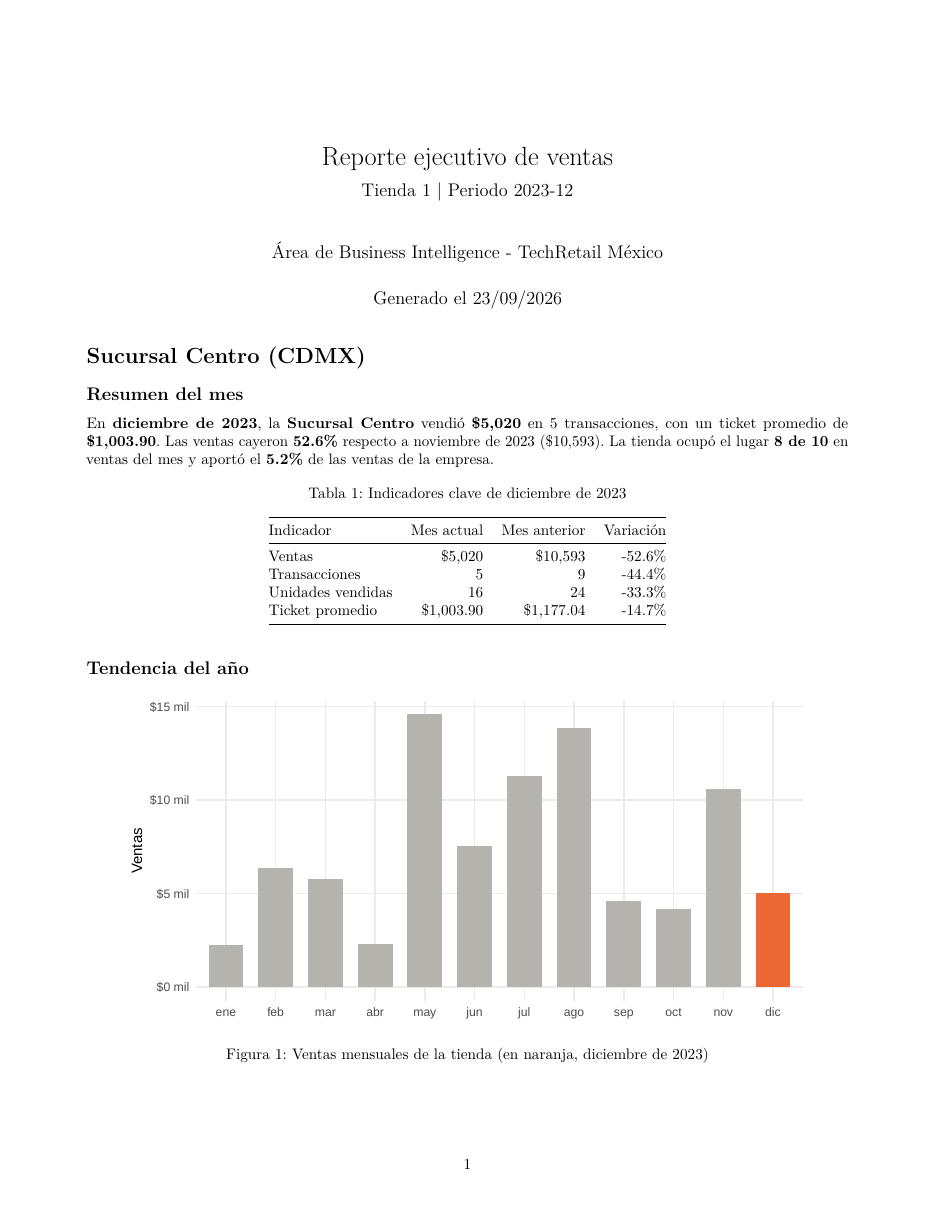
\includegraphics[width=0.47\textwidth]{m08-reporte-ejecutivo}}\hfill
\fbox{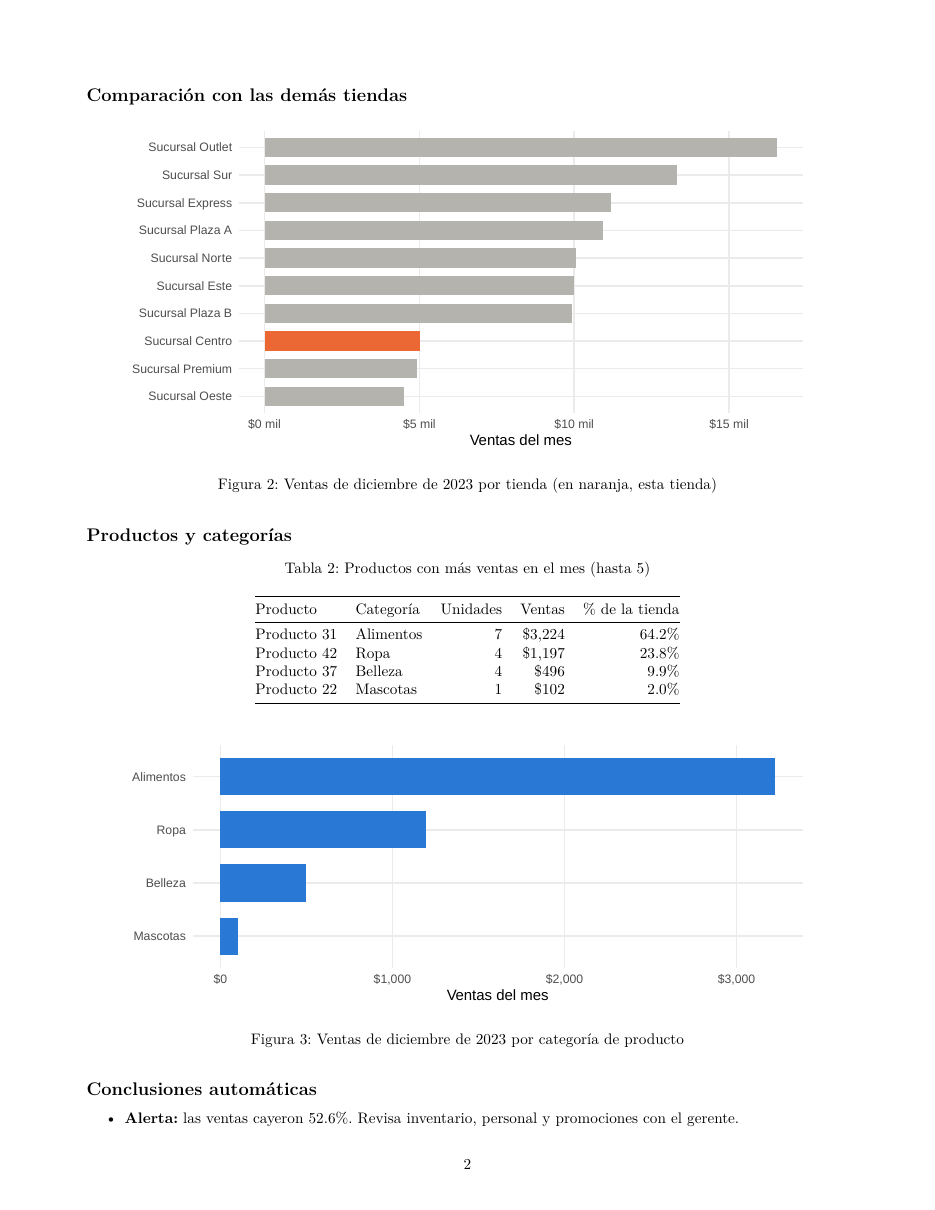
\includegraphics[width=0.47\textwidth]{m08-reporte-ejecutivo-p2}}
\caption{Páginas 1 y 2 del reporte ejecutivo en PDF generado para la
Sucursal Centro, diciembre de 2023.}
\label{fig:m08-reporte-ejecutivo}
\end{figure}

La tercera página contiene el final de las conclusiones automáticas. Para
esta tienda, el reporte escribió:

\begin{textocodigo}
- Alerta: las ventas cayeron 52.6%. Revisa inventario, personal y
  promociones con el gerente.
- La tienda está entre las 3 con menores ventas (lugar 8 de 10).
- El ticket promedio ($1,003.90) es menor que el de la empresa
  ($1,059.27): hay espacio para venta cruzada.
- Precaución: el mes solo tiene 5 transacciones; interpreta las
  variaciones con cuidado.
\end{textocodigo}

El mismo archivo produce la versión HTML (con índice flotante) y la de Word
(editable), sin cambiar una línea: basta con
\codigo{output\_format = "all"}.

\subsection{Generar los diez reportes}

Con la carpeta del curso como directorio de trabajo, en la terminal
(o en la pestaña \menu{Terminal} de RStudio):

\begin{textocodigo}
Rscript reportes/generar_reportes.R 2023-12 pdf
\end{textocodigo}

\begin{textocodigo}[title=Salida real del script]
Generando 10 reportes del mes 2023-12 en formato pdf
  [ 1/10] Sucursal Centro    OK    2023-12_T01_sucursal-centro_2026-09-23.pdf
  [ 2/10] Sucursal Norte     OK    2023-12_T02_sucursal-norte_2026-09-23.pdf
  [ 3/10] Sucursal Sur       OK    2023-12_T03_sucursal-sur_2026-09-23.pdf
  ...
  [10/10] Sucursal Express   OK    2023-12_T10_sucursal-express_2026-09-23.pdf

Listo: 10 reportes generados, 0 con error. Carpeta: .../resultados/reportes
Registro guardado en: .../resultados/reportes/registro_reportes.csv
\end{textocodigo}

En unos 20 segundos, los diez PDF están en \archivo{resultados/reportes/}.
Si ejecutas el script para un mes sin datos, por ejemplo
\codigo{Rscript reportes/generar\_reportes.R 2024-01}, ningún reporte se
genera, pero el script no se detiene en la primera tienda: recorre las diez,
y el registro explica la causa:

\begin{textocodigo}[title=resultados/reportes/registro\_reportes.csv (extracto)]
fecha_hora,tienda_id,tienda,mes,archivo,estado,detalle,segundos
2026-09-23 22:02:00,1,Sucursal Centro,2023-12,2023-12_T01_sucursal-centro_2026-09-23.pdf,OK,OK,2.2
...
2026-09-23 22:02:28,1,Sucursal Centro,2024-01,2024-01_T01_sucursal-centro_2026-09-23.html,ERROR,ERROR: No hay datos del mes 2024-01,0.4
\end{textocodigo}

\begin{hazlotu}
Genera los reportes de junio de 2023 en Word para todas las tiendas. Abre el
de la tienda que tuvo el mayor crecimiento y comprueba que su conclusión
dice ``Crecimiento sólido''. Luego revisa \archivo{registro\_reportes.csv}:
¿cuántas filas tiene ahora y por qué?
\end{hazlotu}

% ----------------------------------------------------------------------------
\section{Errores comunes}
\label{sec:m8-errores}

Estos son los errores que casi todo el mundo encuentra en sus primeros
reportes. Los mensajes son los que muestra R (con las rutas acortadas).

\begin{advertencia}
\textbf{Archivo de datos no encontrado al hacer Knit.} El código funciona
en la consola, pero al tejer aparece:
\end{advertencia}

\begin{textocodigo}
Quitting from lines 7-9 [cargar] (reporte.Rmd)
Error:
! 'datasets/ventas_retail.csv' does not exist in current working
  directory ('.../curso-bi-rstudio/reportes').
\end{textocodigo}

\textbf{Causa:} el \archivo{.Rmd} se ejecuta en su propia carpeta
(\archivo{reportes/}), no en la del proyecto. \textbf{Solución:} usa
\codigo{knit\_root\_dir} en \codigo{render()} o
\menu{Knit > Knit Directory > Project Directory}, una ruta
\archivo{../datasets/}, el paquete \paquete{here} o la búsqueda robusta con
el parámetro \codigo{ruta\_datos} (sección~\ref{sec:m8-directorio}). El
mensaje te dice cuál es el directorio de trabajo real: léelo.

\begin{advertencia}
\textbf{Objeto no encontrado (pero en la consola sí existe).}
\end{advertencia}

\begin{textocodigo}
Quitting from lines 7-8 [resumen] (reporte.Rmd)
Error:
! objeto 'ventas' no encontrado
\end{textocodigo}

\textbf{Causa:} Knit ejecuta el documento en una \emph{sesión nueva y
limpia}. El objeto \codigo{ventas} existe en tu consola porque lo creaste
ahí, pero el \archivo{.Rmd} nunca lo crea. \textbf{Solución:} el
\archivo{.Rmd} debe leer sus datos y cargar sus paquetes (\codigo{library()})
él mismo. Prueba: reinicia R (\menu{Session > Restart R}) y ejecuta todos
los bloques en orden con \menu{Run > Run All}; si falla ahí, fallará al
tejer. Lo mismo ocurre con \codigo{could not find function "\%>\%"}: falta
un \codigo{library(dplyr)} dentro del documento.

\begin{advertencia}
\textbf{Falta LaTeX para generar PDF.}
\end{advertencia}

\begin{textocodigo}
! sh: 1: pdflatex: not found

Error: LaTeX failed to compile reporte.tex. See
https://yihui.org/tinytex/r/#debugging for debugging tips.
\end{textocodigo}

En Windows el mensaje suele ser \emph{``No LaTeX installation detected
(LaTeX is required to create PDF output)''}. \textbf{Solución:}
\codigo{tinytex::install\_tinytex()} y reinicia RStudio. Si ya tienes
TinyTeX y el error menciona un archivo \archivo{.sty} faltante, ejecuta de
nuevo el render con Internet para que se descargue.

\begin{advertencia}
\textbf{Nombre de chunk duplicado.}
\end{advertencia}

\begin{textocodigo}
Error in parse_block(g[-1], g[1], params.src, markdown_mode) :
  Duplicate chunk label 'grafica', which has been used for the chunk:
plot(1:10)
\end{textocodigo}

\textbf{Causa:} dos bloques tienen el mismo nombre (pasa mucho al copiar y
pegar un bloque). \textbf{Solución:} cada nombre debe ser único; renombra el
segundo (\codigo{grafica-tiendas}).

\begin{advertencia}
\textbf{Error de YAML por sangría.}
\end{advertencia}

\begin{textocodigo}
Error in yaml::yaml.load(..., eval.expr = TRUE) :
  Scanner error: mapping values are not allowed in this context at
  line 5, column 11
\end{textocodigo}

El encabezado que lo produjo tenía un espacio de más antes de
\codigo{theme}:

\begin{textocodigo}
output:
  html_document:
    toc: true
     theme: flatly
\end{textocodigo}

\textbf{Solución:} alinea las opciones del mismo nivel exactamente con la
misma sangría (múltiplos de dos espacios, sin tabuladores). El mensaje
indica la línea y columna \emph{dentro del YAML}. Otros errores de YAML
frecuentes: olvidar los dos puntos, o escribir un título con dos puntos sin
comillas (\codigo{title: Ventas: diciembre}).

\begin{advertencia}
\textbf{Modificar un parámetro.} \codigo{params\$tienda <- 5} dentro del
documento produce \emph{``no se puede cambiar el valor de un vínculo
bloqueado para `params'\,''}. Copia el parámetro a otra variable.
\end{advertencia}

\begin{table}[H]
\centering
\caption{Otros problemas frecuentes y su solución}
\label{tab:m8-otros-errores}
\small
\begin{tabularx}{\textwidth}{X X}
\toprule
\textbf{Síntoma} & \textbf{Solución} \\
\midrule
El reporte sale con mensajes de carga de paquetes y advertencias &
  \codigo{message = FALSE, warning = FALSE} en \codigo{opts\_chunk\$set()} \\
Cada reporte del bucle sobrescribe al anterior & Da un
  \codigo{output\_file} distinto en cada vuelta \\
La tabla sale como texto de consola (con \codigo{\#\#}) & Usa
  \codigo{kable()} en lugar de imprimir el data frame \\
El texto de \codigo{cat()} aparece en un recuadro gris & Agrega
  \codigo{results = "asis"} al bloque \\
Los meses salen en inglés & Usa un vector propio con los nombres en
  español \\
Los números de un reporte ``se parecen'' a los de otra tienda & Usa
  \codigo{envir = new.env()} en \codigo{render()} \\
\bottomrule
\end{tabularx}
\end{table}

% ----------------------------------------------------------------------------
\begin{resumen}
\begin{itemize}
  \item Un \textbf{reporte reproducible} se genera por completo desde los
        datos y el código: sin copiar y pegar, sin errores de transcripción,
        y se actualiza con un clic.
  \item Un \archivo{.Rmd} tiene \textbf{encabezado YAML}, \textbf{texto en
        Markdown}, \textbf{chunks} de código y \textbf{código en línea}.
        \paquete{knitr} ejecuta el código y \textbf{pandoc} lo convierte a
        HTML, PDF (vía LaTeX) o Word.
  \item Las \textbf{opciones de chunk} controlan qué se ve:
        \codigo{echo}, \codigo{include}, \codigo{message},
        \codigo{fig.cap}, \codigo{results = "asis"}; se fijan para todo el
        documento con \codigo{knitr::opts\_chunk\$set()}.
  \item \codigo{kable()} convierte data frames en tablas de documento;
        \paquete{scales} da formato de negocio a números y porcentajes.
  \item El \textbf{texto dinámico} y las \textbf{conclusiones automáticas}
        (\codigo{if}/\codigo{else}, \codigo{case\_when()}) hacen que la
        narrativa cambie con los datos.
  \item Los \textbf{parámetros} (\codigo{params}) convierten un
        \archivo{.Rmd} en una plantilla; \codigo{render()} con
        \codigo{params}, \codigo{output\_file} y \codigo{knit\_root\_dir}
        genera cada versión.
  \item Un script con un bucle, \codigo{tryCatch()} y un registro genera
        todos los reportes; \textbf{cron} o el \textbf{Programador de tareas}
        lo ejecutan solos, y \paquete{blastula} los envía por correo.
  \item \paquete{writexl} crea libros de Excel con varias hojas a partir de
        una lista de data frames. \textbf{Quarto} (\archivo{.qmd}) es el
        sucesor de R Markdown y usa casi la misma sintaxis.
\end{itemize}
\end{resumen}

\begin{table}[H]
\centering
\caption{Funciones y opciones clave del Módulo 8}
\label{tab:m8-funciones}
\small
\begin{tabularx}{\textwidth}{l X}
\toprule
\textbf{Función u opción} & \textbf{Para qué sirve} \\
\midrule
\codigo{rmarkdown::render()} & Genera el reporte desde código (lo que hace
  el botón Knit) \\
\codigo{params = list(...)} & Valores de los parámetros del reporte \\
\codigo{knit\_root\_dir}, \codigo{output\_dir}, \codigo{output\_file} &
  Carpeta de ejecución, carpeta y nombre de salida \\
\codigo{knitr::opts\_chunk\$set()} & Opciones por defecto de todos los
  chunks \\
\codigo{echo}, \codigo{include}, \codigo{eval}, \codigo{message},
  \codigo{warning} & Qué se muestra y qué se ejecuta \\
\codigo{fig.cap}, \codigo{fig.width}, \codigo{fig.height},
  \codigo{out.width} & Título y tamaño de las figuras \\
\codigo{results = "asis"} & El texto impreso se trata como Markdown \\
\codigo{knitr::kable()} & Tabla con formato de documento \\
\codigo{knitr::knit()} & Teje un documento (o un texto) a Markdown \\
\codigo{knitr::pandoc\_to()} & Formato de salida que se está generando \\
\codigo{dollar()}, \codigo{percent()}, \codigo{comma()} & Formato de
  números en texto y tablas \\
\codigo{tryCatch()} & Atrapa errores para que el bucle continúe \\
\codigo{sprintf()} & Arma nombres de archivo con un molde \\
\codigo{expand\_grid()} & Todas las combinaciones de parámetros \\
\codigo{commandArgs()} & Lee los argumentos de \codigo{Rscript} \\
\codigo{writexl::write\_xlsx()} & Excel con una hoja por data frame \\
\codigo{readxl::excel\_sheets()} & Nombres de las hojas de un Excel \\
\codigo{tinytex::install\_tinytex()} & Instala LaTeX para generar PDF \\
\bottomrule
\end{tabularx}
\end{table}

% ----------------------------------------------------------------------------
\section{Ejercicios}
\label{sec:m8-ejercicios}

Para los ejercicios que piden un archivo \archivo{.Rmd}, guárdalo en la
carpeta \archivo{reportes/} del curso y genéralo con \menu{Knit} o con
\codigo{rmarkdown::render()}. Los demás se resuelven con código R en la
consola, con la carpeta del curso como directorio de trabajo.

\begin{ejercicio}{m8-1}{Tu primer reporte de clientes}
\nivel{Básico}
Crea \archivo{reportes/ej1-clientes.Rmd} con salida HTML que:
(a) tenga título, tu nombre y la fecha automática;
(b) lea \archivo{clientes.csv} en un bloque que no se muestre en el
reporte;
(c) diga en una frase, con código en línea, cuántos clientes hay y cuántos
son premium;
(d) muestre una tabla con \codigo{kable()} del número de clientes por
\codigo{ciudad}, ordenada de mayor a menor.
\end{ejercicio}

\begin{ejercicio}{m8-2}{Tabla ejecutiva de categorías}
\nivel{Básico}
Con \archivo{transacciones.csv} y \archivo{productos.csv}, construye una
tabla con \codigo{kable(format = "pipe")} de las ventas de 2023 por
\codigo{categoria}: ventas en pesos sin centavos, unidades con separador de
miles y porcentaje del total con un decimal, ordenada de mayor a menor y con
el título ``Ventas 2023 por categoría''. ¿Qué categoría vende más y qué
porcentaje representa?
\end{ejercicio}

\begin{ejercicio}{m8-3}{Frase de cumplimiento de meta}
\nivel{Intermedio}
Escribe una función \codigo{frase\_meta(ventas, meta)} que devuelva:
``Se superó la meta en X\,\% (ventas de \$A contra meta de \$B).'' si
\codigo{ventas >= meta}; ``Se alcanzó el X\,\% de la meta\ldots'' si se
alcanzó al menos el 90\,\%; y ``Alerta: solo se alcanzó el X\,\% de la
meta\ldots'' en otro caso. Pruébala con los tres casos y aplícala a las
ventas trimestrales de 2023 (de \archivo{transacciones.csv}) con una meta de
\$220,000 por trimestre.
\end{ejercicio}

\begin{ejercicio}{m8-4}{Opciones de chunk para un reporte ejecutivo}
\nivel{Intermedio}
Crea \archivo{reportes/ej4-opciones.Rmd} con un bloque de configuración
global que oculte código, mensajes y advertencias. Incluye: un bloque
invisible que calcule las ventas por mes de \archivo{ventas\_retail.csv};
una gráfica de líneas con \codigo{fig.cap}, 7 $\times$ 3 pulgadas y
\codigo{out.width = "80\%"}; y un bloque con \codigo{results = "asis"} que
escriba como lista de Markdown los tres meses con más ventas. Genéralo en
HTML y en Word.
\end{ejercicio}

\begin{ejercicio}{m8-5}{Reporte parametrizado por categoría}
\nivel{Intermedio}
Crea \archivo{reportes/ej5-categoria.Rmd} con un parámetro
\codigo{categoria} (valor por defecto \codigo{"Electrónica"}) que muestre,
para esa categoría: ventas totales de 2023 (en una frase), una tabla de sus
5 productos más vendidos y una gráfica de ventas por mes. Después genera,
con \codigo{render()}, los reportes de \codigo{"Ropa"} y \codigo{"Hogar"}
con nombres de archivo distintos en \archivo{resultados/}.
\end{ejercicio}

\begin{ejercicio}{m8-6}{Plan de generación por trimestre}
\nivel{Avanzado}
Construye con \codigo{expand\_grid()} la tabla de trabajos para generar un
reporte por tienda y por trimestre (\codigo{Q1} a \codigo{Q4}). Agrega una
columna \codigo{archivo} con el formato
\archivo{2023-Q1\_T01\_sucursal-centro.pdf} y una columna
\codigo{n\_transacciones} con cuántas transacciones tiene cada combinación
(según \archivo{transacciones.csv}). ¿Cuántos reportes hay que generar?
¿Qué combinación tiene menos transacciones? Marca con
\codigo{generar = FALSE} las que tengan menos de 20.
\end{ejercicio}

\begin{ejercicio}{m8-7}{Un Excel con una hoja por tienda}
\nivel{Avanzado}
Genera \archivo{resultados/ventas\_por\_tienda.xlsx} con una hoja
\codigo{"Resumen"} (ventas y transacciones por tienda) seguida de una hoja
por tienda con el detalle de sus transacciones, cuyo nombre sea el de la
tienda sin la palabra ``Sucursal'' (por ejemplo, \codigo{"Centro"}). Pista:
\codigo{split()} divide un data frame en una lista. Verifica con
\codigo{excel\_sheets()} que hay 11 hojas y que la suma de filas de las
hojas de tiendas es 1,000.
\end{ejercicio}

\begin{ejercicio}{m8-8}{Sistema de alertas con registro}
\nivel{Reto}
Escribe una función \codigo{revisar\_tienda(id, mes)} que calcule la
variación de ventas de una tienda contra el mes anterior y devuelva un
tibble de una fila con la tienda, el mes, la variación y un estado
(``Crecimiento sólido'', ``Estable'', ``Ligera caída'', ``Alerta''), y que
lance un error con \codigo{stop()} si la tienda o el mes no existen, o si el
mes anterior no tiene datos. Recorre todas las tiendas para
\codigo{"2023-06"}, más las combinaciones inválidas \codigo{(11, "2023-06")}
y \codigo{(1, "2023-01")}, atrapando los errores con \codigo{tryCatch()}.
Muestra el registro y escribe con \codigo{cat()} el texto Markdown de
alertas que iría en el reporte.
\end{ejercicio}


\part{Proyecto integrador}
% ============================================================================
% MÓDULO 9 - PROYECTO FINAL: TECHRETAIL MÉXICO
% ============================================================================
\chapter{Proyecto final: TechRetail México}
\label{cap:proyecto}

\begin{objetivos}
\begin{itemize}
  \item Plantear un proyecto de Business Intelligence completo a partir de un
        reto de negocio real: preguntas, entregables, cronograma y criterios
        de evaluación.
  \item Construir un proceso ETL auditable: cargar varias fuentes, detectar
        problemas de calidad, documentar cada decisión de limpieza y armar un
        modelo en estrella listo para analizar.
  \item Calcular los KPIs de la empresa y convertir cada tabla o gráfica en
        un hallazgo de negocio con números reales.
  \item Aplicar segmentación de clientes y pronóstico de ventas siendo honesto
        sobre lo que los datos permiten (y lo que no).
  \item Diseñar el tablero ejecutivo, redactar el reporte para la dirección y
        preparar la presentación de resultados.
  \item Organizar el proyecto de forma reproducible y presentarlo en tu
        portafolio para buscar trabajo en BI.
\end{itemize}
\end{objetivos}

Llegaste al final del curso. Ya sabes importar y transformar datos
(Módulo~\ref{cap:manipulacion}), graficarlos con criterio
(Módulo~\ref{cap:visualizacion}), explorarlos con estadística
(Módulo~\ref{cap:eda}), guardarlos en una base de datos
(Módulo~\ref{cap:bases-datos}), construir tableros interactivos
(Módulo~\ref{cap:shiny}), entrenar modelos (Módulo~\ref{cap:ml}) y
automatizar reportes (Módulo~\ref{cap:reportes}). Cada módulo resolvió una
pieza. En la vida real nadie te pide ``una pieza'': te piden \emph{resolver un
problema de negocio}, y tú decides qué herramientas usar, en qué orden y cómo
comunicar lo que encontraste.

Este módulo simula exactamente eso. Vas a trabajar como consultor de BI para
\textbf{TechRetail México}, una cadena de diez sucursales que tiene un año de
datos y muchas preguntas. No vamos a re-enseñar técnicas: cada vez que uses
algo que ya aprendiste, te remitiremos al módulo donde se explicó y nos
concentraremos en lo que distingue a un analista junior de uno senior: el
\emph{razonamiento de negocio}, las \emph{decisiones} (y su justificación) y la
\emph{comunicación} de resultados.

Una advertencia honesta antes de empezar: los datos del curso son simulados.
Eso significa que algunos patrones que esperarías en una tienda real (más
ventas en diciembre, fines de semana más fuertes, clientes premium que gastan
más) pueden no aparecer, o aparecer por azar. Lejos de ser un problema, es un
excelente entrenamiento: aprenderás a decir ``los datos no muestran
diferencia'' con la misma seguridad con la que dirías ``encontramos una
oportunidad de un millón de pesos''. Un buen analista no fuerza conclusiones.

\begin{concepto}{Proyecto integrador de BI}
Un \termino{proyecto integrador} recorre el ciclo completo de la
inteligencia de negocios: \emph{pregunta de negocio} $\rightarrow$
\emph{datos} (ETL) $\rightarrow$ \emph{análisis} (KPIs, exploración,
modelos) $\rightarrow$ \emph{producto} (tablero, reporte) $\rightarrow$
\emph{decisión} (presentación y recomendaciones). El valor no está en
ninguna etapa aislada, sino en que la cadena completa lleve de un dato crudo
a una acción concreta de la dirección.
\end{concepto}

\begin{figure}[H]
\centering
\begin{tikzpicture}[
    fase/.style={draw=primario, fill=primario!6, rounded corners=3pt,
                 minimum width=4.4cm, minimum height=1.45cm, align=center,
                 font=\small\sffamily},
    flecha/.style={-{Stealth[length=2.5mm]}, thick, color=acento}]
  \node[fase] (f1) {\textbf{Fase 1. ETL y modelo}\\ Módulos \ref{cap:manipulacion} y \ref{cap:bases-datos}};
  \node[fase, right=0.9cm of f1] (f2) {\textbf{Fase 2. KPIs y exploración}\\ Módulos \ref{cap:visualizacion} y \ref{cap:eda}};
  \node[fase, right=0.9cm of f2] (f3) {\textbf{Fase 3. Segmentación}\\ \textbf{y pronóstico}\\ Módulo \ref{cap:ml}};
  \node[fase, below=1.1cm of f3] (f4) {\textbf{Fase 4. Dashboard}\\ Módulo \ref{cap:shiny}};
  \node[fase, left=0.9cm of f4] (f5) {\textbf{Fase 5. Reporte ejecutivo}\\ Módulo \ref{cap:reportes}};
  \node[fase, left=0.9cm of f5] (f6) {\textbf{Fase 6. Presentación}\\ Storytelling con datos};
  \draw[flecha] (f1) -- (f2);
  \draw[flecha] (f2) -- (f3);
  \draw[flecha] (f3) -- (f4);
  \draw[flecha] (f4) -- (f5);
  \draw[flecha] (f5) -- (f6);
\end{tikzpicture}
\caption{Las seis fases del proyecto y los módulos del libro que usa cada una.}
\label{fig:m09-fases}
\end{figure}

% ============================================================================
\section{El caso: TechRetail México}
\label{sec:m09-caso}
% ============================================================================

TechRetail México es una cadena minorista con diez sucursales en seis
ciudades del país. Vende productos de diez categorías (desde electrónica y
juguetes hasta alimentos y artículos para mascotas) y registra cada venta en
un sistema de punto de venta. La dirección tiene los datos de 2023 pero nunca
los ha analizado de forma integral: cada gerente de tienda lleva su propio
Excel, y las juntas de resultados terminan en discusiones sobre ``qué número
es el bueno''.

Antes de escribir una sola línea de análisis, prepara el entorno del
proyecto. Fíjate en la \termino{fecha de corte}: es la fecha ``de hoy'' para
el proyecto. El script original del curso usaba \codigo{Sys.Date()}, lo que
hace que los resultados cambien cada día que lo ejecutas (la antigüedad de
una tienda o los días desde la última compra de un cliente serían distintos
mañana). En un proyecto profesional eso es inaceptable: quien revise tu
trabajo dentro de seis meses debe obtener exactamente los mismos números.

\begin{rcode}[title=Configuración del proyecto]
# ---- Paquetes (todos se explicaron en módulos anteriores) ----
library(tidyverse)   # dplyr, ggplot2, readr, tidyr, purrr, lubridate
library(scales)      # formatos de negocio: dollar(), percent(), comma()
library(DBI)         # interfaz a bases de datos (Módulo 5)
library(RSQLite)     # motor SQLite en un archivo local
library(cluster)     # silueta para evaluar k-means (Módulo 7)
library(forecast)    # modelos de pronóstico (Módulo 7)

# ---- Fecha de corte FIJA (nunca Sys.Date() en un proyecto) ----
fecha_corte <- as.Date("2024-01-01")

# ---- Carpetas de salida del proyecto ----
dir.create("resultados", showWarnings = FALSE)
dir.create("datos", showWarnings = FALSE)

# ---- Colores corporativos y tema (los mismos del Módulo 3) ----
color_principal <- "#2a78d6"   # una sola serie
color_resalte   <- "#eb6834"   # lo que queremos destacar
color_gris      <- "#b5b3ad"   # el resto
paleta_libro <- c("#2a78d6", "#eb6834", "#1baf7a", "#eda100",
                  "#e87ba4", "#008300", "#4a3aa7", "#e34948")

tema_libro <- function(base_size = 11) {
  theme_minimal(base_size = base_size) +
    theme(
      plot.title       = element_text(face = "bold", color = "#0b0b0b"),
      plot.subtitle    = element_text(color = "#52514e"),
      plot.caption     = element_text(color = "#52514e", size = rel(0.8)),
      axis.title       = element_text(color = "#52514e"),
      axis.text        = element_text(color = "#52514e"),
      panel.grid.minor = element_blank(),
      panel.grid.major = element_line(color = "#e6e5e1", linewidth = 0.3),
      legend.position  = "top",
      legend.title     = element_text(color = "#52514e")
    )
}

# Formato de pesos sin decimales para textos y tablas
pesos <- function(x) dollar(x, accuracy = 1)
\end{rcode}

Al cargar \paquete{tidyverse} y \paquete{forecast} verás mensajes de
bienvenida o avisos como \codigo{Registered S3 method overwritten}; son
normales y no indican ningún error.

\subsection{La cadena en números}

Describe a la empresa con sus propios datos, no con adjetivos. El archivo
\archivo{tiendas.csv} es el catálogo de sucursales.

\begin{rcode}
tiendas <- read_csv("datasets/tiendas.csv", show_col_types = FALSE)

# Antigüedad de cada sucursal calculada a la fecha de corte
tiendas %>%
  mutate(anios = floor(time_length(
           interval(fecha_apertura, fecha_corte), "years"))) %>%
  select(tienda = nombre_tienda, ciudad, zona, tipo,
         m2 = tamano_m2, empleados, anios) %>%
  arrange(desc(m2))
\end{rcode}

\begin{rsalida}
# A tibble: 10 x 7
   tienda           ciudad      zona   tipo         m2 empleados anios
   <chr>            <chr>       <chr>  <chr>     <dbl>     <dbl> <dbl>
 1 Sucursal Premium CDMX        Sur    Premium     800        40    14
 2 Sucursal Plaza A CDMX        Oeste  Principal   700        35     7
 3 Sucursal Sur     Monterrey   Norte  Estándar    600        30    12
 4 Sucursal Oeste   Puebla      Centro Estándar    550        22    10
 5 Sucursal Centro  CDMX        Centro Principal   500        25    13
 6 Sucursal Plaza B Guadalajara Norte  Estándar    480        21     9
 7 Sucursal Norte   Guadalajara Norte  Estándar    450        20    11
 8 Sucursal Este    CDMX        Este   Estándar    400        18     8
 9 Sucursal Outlet  Tijuana     Norte  Outlet      350        15     5
10 Sucursal Express Querétaro   Centro Express     300        12     3
\end{rsalida}

\begin{rcode}
# Resumen de la red de sucursales
tiendas %>%
  summarise(sucursales = n(),
            ciudades   = n_distinct(ciudad),
            m2_totales = sum(tamano_m2),
            empleados  = sum(empleados),
            m2_por_empleado = round(sum(tamano_m2) / sum(empleados), 1))

tiendas %>% count(ciudad, sort = TRUE)
\end{rcode}

\begin{rsalida}
# A tibble: 1 x 5
  sucursales ciudades m2_totales empleados m2_por_empleado
       <int>    <int>      <dbl>     <dbl>           <dbl>
1         10        6       5130       238            21.6
# A tibble: 6 x 2
  ciudad          n
  <chr>       <int>
1 CDMX            4
2 Guadalajara     2
3 Monterrey       1
4 Puebla          1
5 Querétaro       1
6 Tijuana         1
\end{rsalida}

¿Qué nos dice esto? TechRetail tiene 10 sucursales en 6 ciudades, con
5,130~m\textsuperscript{2} de piso de venta y 238 empleados. La Ciudad de
México concentra 4 sucursales, incluidas la más grande (Sucursal Premium,
800~m\textsuperscript{2} y 40 empleados, la más antigua: 14 años) y la
Sucursal Plaza A. En el otro extremo están la Sucursal Express de Querétaro
(300~m\textsuperscript{2}, abierta en 2020) y la Sucursal Outlet de Tijuana.
Hay cinco formatos (Principal, Estándar, Outlet, Premium y Express), lo cual
será importante: no es justo comparar las ventas absolutas de una tienda de
800~m\textsuperscript{2} con las de una de 300.

\begin{advertencia}
Observa que la ``Sucursal Sur'' está en Monterrey y pertenece a la zona
\emph{Norte}. Los nombres heredados no siempre describen la realidad. En el
análisis usaremos siempre la columna \codigo{zona}, nunca el nombre de la
tienda, para agrupar geográficamente.
\end{advertencia}

\subsection{El reto de la dirección}

\begin{negocio}{El correo de la directora general}
\emph{``Necesitamos dejar de discutir números y empezar a tomar decisiones.
Quiero, en seis semanas: (1) una sola versión de la verdad de nuestras ventas
de 2023, (2) entender qué tiendas, productos y clientes nos hacen ganar
dinero, (3) un tablero que los gerentes consulten cada lunes y (4) una
recomendación clara de en qué enfocarnos en 2024. Preséntalo al comité
directivo en 20 minutos.''}

Traducido a BI: la dirección pide \textbf{calidad y gobierno de datos} (una
sola versión de la verdad), \textbf{análisis descriptivo y diagnóstico}
(qué pasó y por qué), un \textbf{producto de datos recurrente} (tablero) y
\textbf{recomendaciones accionables} (presentación y reporte).
\end{negocio}

\subsection{Las 20 preguntas de negocio}

El primer entregable de cualquier consultoría es la lista de preguntas que
vas a contestar, acordada con el cliente. Evita el ``análisis de todo'': si
una tabla no responde una pregunta, sobra. La
Tabla~\ref{tab:m09-preguntas} agrupa las 20 preguntas en cuatro áreas e
indica dónde se responde cada una en este módulo.

\begin{table}[H]
\centering
\small
\caption{Las 20 preguntas de negocio del proyecto y dónde se responden.}
\label{tab:m09-preguntas}
\begin{tabularx}{\textwidth}{@{}c X l@{}}
\toprule
\# & Pregunta & Dónde se responde \\
\midrule
\multicolumn{3}{@{}l}{\textbf{Ventas}} \\
1 & ¿Cuánto vendimos en 2023, en cuántas transacciones y con qué ticket promedio? & Sec.~\ref{sec:m09-kpis-globales} \\
2 & ¿Cómo evolucionaron las ventas mes a mes? ¿Estamos creciendo? & Sec.~\ref{sec:m09-mensual} \\
3 & ¿Qué categorías generan más ingresos y más margen? & Sec.~\ref{sec:m09-categorias} \\
4 & ¿Qué método de pago prefieren los clientes y cambia el ticket? & Sec.~\ref{sec:m09-pago} \\
5 & ¿Qué ventas podemos esperar en las próximas semanas? & Sec.~\ref{sec:m09-pronostico} \\
\midrule
\multicolumn{3}{@{}l}{\textbf{Clientes}} \\
6 & ¿Cuántos clientes activos tenemos y cuántos no compraron? & Sec.~\ref{sec:m09-kpis-globales} \\
7 & ¿Los clientes premium gastan más que los demás? & Sec.~\ref{sec:m09-premium} \\
8 & ¿Qué segmentos de clientes existen según su comportamiento? & Sec.~\ref{sec:m09-rfm} \\
9 & ¿Cuántos clientes vuelven a comprar y cada cuánto? & Reto~\ref{ej:p-1} \\
10 & ¿Se comportan distinto los clientes según el mes en que llegaron? & Reto~\ref{ej:p-4} \\
\midrule
\multicolumn{3}{@{}l}{\textbf{Productos}} \\
11 & ¿Pocos productos concentran la mayoría de las ventas (Pareto)? & Sec.~\ref{sec:m09-pareto} \\
12 & ¿Qué productos tienen margen negativo en el catálogo? & Sec.~\ref{sec:m09-auditoria} \\
13 & ¿Vendemos al precio de catálogo? & Sec.~\ref{sec:m09-auditoria} \\
14 & ¿Se venden productos marcados como inactivos? & Sec.~\ref{sec:m09-auditoria} \\
15 & ¿Qué productos necesitan reabastecerse pronto? & Reto~\ref{ej:p-3} \\
\midrule
\multicolumn{3}{@{}l}{\textbf{Operaciones}} \\
16 & ¿Qué sucursales y zonas venden más? & Sec.~\ref{sec:m09-tiendas} \\
17 & ¿Qué sucursales son más productivas por m\textsuperscript{2} y por empleado? & Reto~\ref{ej:p-2} \\
18 & ¿Qué días y horas concentran las ventas? & Sec.~\ref{sec:m09-dia-hora} \\
19 & ¿Qué vendedores venden más y se relaciona con su salario? & Sec.~\ref{sec:m09-vendedores} \\
20 & ¿Hay transacciones atípicas que debamos revisar? & Reto~\ref{ej:p-5} \\
\bottomrule
\end{tabularx}
\end{table}

\begin{consejo}
Escribe las preguntas \emph{antes} de abrir los datos y pídele a la dirección
que las priorice. Si al final del proyecto alguien pregunta ``¿y esto para
qué sirve?'', debes poder señalar qué pregunta responde cada gráfica.
\end{consejo}

\subsection{Entregables y cronograma}

El proyecto se organiza en seis fases con un entregable concreto cada una
(Tabla~\ref{tab:m09-cronograma}). Las horas son una estimación para alguien
que termina este libro; en una empresa real, la Fase~1 suele consumir
más tiempo del que todos esperan.

\begin{table}[H]
\centering
\small
\caption{Cronograma del proyecto por fases.}
\label{tab:m09-cronograma}
\begin{tabularx}{\textwidth}{@{}l X X c c@{}}
\toprule
Fase & Actividades principales & Entregable & Semana & Horas \\
\midrule
1. ETL y modelo & Cargar fuentes, auditar calidad, limpiar, modelo en estrella & Datos limpios (RDS y SQLite) y bitácora de decisiones & 1 & 5--6 \\
2. KPIs y exploración & KPIs globales, tendencias, cortes por tienda, producto, cliente y vendedor & Diccionario de KPIs y cuaderno de hallazgos & 2 & 5--6 \\
3. Modelos & Segmentación RFM con k-means y pronóstico de ventas & Segmentos con acciones y pronóstico con intervalos & 3 & 4--5 \\
4. Dashboard & Diseño y construcción del tablero en Shiny & App funcionando con filtros & 4 & 4--5 \\
5. Reporte & Reporte ejecutivo automatizado en R Markdown & PDF o HTML de 1--2 páginas & 5 & 2--3 \\
6. Presentación & Guion, diapositivas y ensayo & Presentación de 8--10 diapositivas & 6 & 2--3 \\
\bottomrule
\end{tabularx}
\end{table}

\subsection{Rúbrica de evaluación}

Si usas este proyecto para un curso, un bootcamp o tu portafolio, evalúalo
con criterios explícitos (Tabla~\ref{tab:m09-rubrica}). Observa que el código
vale menos de la mitad: en BI, un análisis técnicamente perfecto que nadie
entiende no sirve.

\begin{table}[H]
\centering
\small
\caption{Rúbrica de evaluación del proyecto final.}
\label{tab:m09-rubrica}
\begin{tabularx}{\textwidth}{@{}l c X X@{}}
\toprule
Criterio & Peso & Excelente & Insuficiente \\
\midrule
Calidad de datos & 15\% & Auditoría con evidencia, decisiones documentadas y justificadas & Se limpian datos ``a ojo'' o se borran filas sin explicar \\
Código y reproducibilidad & 20\% & Scripts numerados, comentados, fecha de corte fija; corre de principio a fin & Rutas absolutas, \codigo{Sys.Date()}, pasos manuales \\
Análisis y KPIs & 25\% & Cada gráfica responde una pregunta y trae un hallazgo con números & Muchas gráficas sin conclusión \\
Modelos & 10\% & Modelo justificado, validado y con limitaciones explícitas & Modelo sin validar o con conclusiones exageradas \\
Tablero y reporte & 15\% & Tablero claro con KPIs y filtros; reporte breve y automatizado & Tablero saturado; reporte copiado a mano \\
Comunicación & 15\% & Historia clara, recomendaciones accionables con impacto & Lista de datos sin recomendación \\
\bottomrule
\end{tabularx}
\end{table}

\begin{hazlotu}
Agrega tres preguntas propias a la Tabla~\ref{tab:m09-preguntas} (por
ejemplo, sobre marcas o proveedores). Para cada una anota qué archivo y qué
columnas necesitarías para responderla.
\end{hazlotu}

% ============================================================================
\section{Fase 1: ETL y modelo de datos}
\label{sec:m09-etl}
% ============================================================================

La primera fase construye la ``única versión de la verdad'' que pidió la
directora. Seguimos las tres letras del \termino{ETL}: \emph{extraer} (leer
las fuentes), \emph{transformar} (auditar, limpiar, enriquecer) y
\emph{cargar} (guardar el resultado en un formato listo para analizar). Las
funciones de \paquete{dplyr} y \paquete{readr} se explicaron en el
Módulo~\ref{cap:manipulacion} y las bases de datos en el
Módulo~\ref{cap:bases-datos}; aquí nos enfocamos en las decisiones.

\subsection{Extraer: cargar las fuentes}

\begin{rcode}
# Tabla de hechos candidata principal: una fila por transacción
transacciones <- read_csv("datasets/transacciones.csv",
                          show_col_types = FALSE)
# Segunda fuente de ventas (una venta registrada por día)
ventas_retail <- read_csv("datasets/ventas_retail.csv",
                          show_col_types = FALSE)
# Catálogos (futuras dimensiones)
clientes  <- read_csv("datasets/clientes.csv",  show_col_types = FALSE)
productos <- read_csv("datasets/productos.csv", show_col_types = FALSE)
empleados <- read_csv("datasets/empleados.csv", show_col_types = FALSE)
# tiendas ya se cargó en la sección anterior

glimpse(transacciones)
\end{rcode}

\begin{rsalida}
Rows: 1,000
Columns: 14
$ transaccion_id    <dbl> 1, 2, 3, 4, 5, 6, 7, 8, 9, 10, 11, 12, 13,~
$ fecha             <date> 2023-01-13, 2023-01-09, 2023-02-20, 2023-~
$ hora              <time> 13:15:00, 10:45:00, 10:30:00, 10:45:00, 1~
$ cliente_id        <dbl> 155, 155, 75, 51, 173, 135, 90, 168, 13, 9~
$ producto_id       <dbl> 3, 47, 6, 17, 28, 46, 30, 48, 21, 12, 49, ~
$ cantidad          <dbl> 4, 4, 3, 4, 1, 2, 4, 2, 2, 5, 2, 3, 4, 2, ~
$ precio_venta      <dbl> 303.97, 58.07, 275.46, 105.28, 205.47, 534~
$ metodo_pago       <chr> "Tarjeta Crédito", "Tarjeta Débito", "Tarj~
$ tienda_id         <dbl> 10, 2, 7, 6, 7, 7, 8, 8, 5, 2, 7, 6, 8, 2,~
$ vendedor_id       <dbl> 4, 22, 14, 5, 14, 22, 23, 5, 3, 14, 5, 9, ~
$ total_transaccion <dbl> 1215.88, 232.28, 826.38, 421.12, 205.47, 1~
$ mes               <chr> "2023-01", "2023-01", "2023-02", "2023-05"~
$ trimestre         <chr> "Q1", "Q1", "Q1", "Q2", "Q1", "Q1", "Q2", ~
$ dia_semana        <chr> "viernes", "lunes", "lunes", "viernes", "m~
\end{rsalida}

Fíjate en un detalle: en el archivo la hora viene como texto sin cero
inicial (\codigo{"8:00"}, \codigo{"13:15"}), pero \paquete{readr} la
reconoció como hora (\codigo{<time>}). Eso nos permitirá extraer la hora del
día con \codigo{hour()} sin conversiones manuales.

\subsection{¿Qué tabla usar como hechos?}
\label{sec:m09-fuente}

Tenemos \emph{dos} archivos de ventas. Antes de sumar nada, compáralos: si
fueran el mismo registro visto de dos formas, sumarlos duplicaría las ventas;
si son registros distintos, necesitamos saber cuál es el oficial.

\begin{rcode}
# Perfil rápido de cada fuente de ventas
perfil_fuente <- function(datos, nombre, col_total) {
  tibble(fuente   = nombre,
         filas    = nrow(datos),
         columnas = ncol(datos),
         desde    = min(datos$fecha),
         hasta    = max(datos$fecha),
         ventas   = sum(datos[[col_total]]))
}

bind_rows(
  perfil_fuente(transacciones, "transacciones", "total_transaccion"),
  perfil_fuente(ventas_retail, "ventas_retail", "total")
)

# ¿Qué información tiene cada fuente que la otra no?
setdiff(names(transacciones), names(ventas_retail))
setdiff(names(ventas_retail), names(transacciones))

# ¿Coinciden registros (misma fecha, cliente y producto)?
inner_join(transacciones, ventas_retail,
           by = c("fecha", "cliente_id", "producto_id")) %>%
  nrow()
\end{rcode}

\begin{rsalida}
# A tibble: 2 x 6
  fuente        filas columnas desde      hasta       ventas
  <chr>         <int>    <int> <date>     <date>       <dbl>
1 transacciones  1000       14 2023-01-01 2023-12-31 959993.
2 ventas_retail   365       14 2023-01-01 2023-12-31 513917.
[1] "transaccion_id"    "hora"              "precio_venta"     
[4] "metodo_pago"       "total_transaccion"
[1] "precio_unitario" "descuento_pct"   "subtotal"       
[4] "descuento_monto" "total"          
[1] 0
\end{rsalida}

Las dos fuentes cubren todo 2023, pero no son el mismo registro: ninguna
combinación de fecha, cliente y producto coincide entre ellas, y los totales
son muy distintos (\$959,993 contra \$513,917). \textbf{Decisión:} usamos
\archivo{transacciones.csv} como tabla de hechos porque (1) es más granular
(1,000 transacciones contra 365 registros, uno por día), (2) trae
información que la otra no tiene y que la dirección pidió (hora, método de
pago) y (3) su total es consistente con su detalle (lo comprobaremos en la
auditoría). \archivo{ventas\_retail.csv} queda como fuente secundaria: es la
única que registra descuentos, así que la usaremos solo para preguntas sobre
promociones (Reto~\ref{ej:p-6}). \textbf{Nunca sumaremos ambas fuentes.}

\begin{advertencia}
Mezclar fuentes de ventas es el error más caro de un proyecto de BI: el
tablero muestra un total que nadie reconoce y el proyecto pierde credibilidad
en la primera junta. Si dos sistemas registran ventas, documenta cuál es el
oficial para cada pregunta y dilo explícitamente en el reporte.
\end{advertencia}

\subsection{Auditoría de calidad de datos}
\label{sec:m09-auditoria}

Una \termino{auditoría de calidad} revisa sistemáticamente cada tabla antes
de usarla: tamaño, faltantes, duplicados, rangos, integridad de llaves y
reglas de negocio. Conviértela en una función para aplicarla igual a todas
las tablas (y reutilizarla cada mes cuando lleguen datos nuevos).

\begin{rcode}
# Auditoría básica de una tabla: tamaño, faltantes y duplicados
auditar <- function(datos, nombre, llave) {
  tibble(
    tabla      = nombre,
    filas      = nrow(datos),
    columnas   = ncol(datos),
    celdas_na  = sum(is.na(datos)),               # valores faltantes
    filas_dup  = sum(duplicated(datos)),          # filas idénticas
    llaves_dup = sum(duplicated(datos[[llave]]))  # llave repetida
  )
}

auditoria <- bind_rows(
  auditar(transacciones, "transacciones", "transaccion_id"),
  auditar(clientes,      "clientes",      "cliente_id"),
  auditar(productos,     "productos",     "producto_id"),
  auditar(tiendas,       "tiendas",       "tienda_id"),
  auditar(empleados,     "empleados",     "empleado_id")
)
auditoria
\end{rcode}

\begin{rsalida}
# A tibble: 5 x 6
  tabla         filas columnas celdas_na filas_dup llaves_dup
  <chr>         <int>    <int>     <int>     <int>      <int>
1 transacciones  1000       14         0         0          0
2 clientes        200       10         0         0          0
3 productos        50       13         0         0          0
4 tiendas          10        8         0         0          0
5 empleados       100       12         0         0          0
\end{rsalida}

Buenas noticias en lo estructural: ninguna tabla tiene valores faltantes,
filas duplicadas ni llaves repetidas. Eso no significa que los datos sean
correctos; significa que están \emph{completos}. Sigue con los rangos y la
consistencia interna de la tabla de hechos.

\begin{rcode}
# Rangos de las columnas clave de la tabla de hechos
rango <- function(x) str_c(min(x), " a ", max(x))
transacciones %>%
  summarise(fecha    = rango(fecha),
            hora     = rango(hms::as_hms(hora)),
            cantidad = rango(cantidad),
            precio   = rango(precio_venta),
            total    = rango(total_transaccion)) %>%
  pivot_longer(everything(), names_to = "columna",
               values_to = "rango")

# ¿El total cuadra con cantidad x precio? (tolerancia de 1 centavo)
transacciones %>%
  summarise(totales_incorrectos =
              sum(abs(total_transaccion - cantidad * precio_venta) > 0.01))
\end{rcode}

\begin{rsalida}
# A tibble: 5 x 2
  columna  rango                  
  <chr>    <chr>                  
1 fecha    2023-01-01 a 2023-12-31
2 hora     28800 a 74700          
3 cantidad 1 a 5                  
4 precio   20.14 a 598.81         
5 total    22.65 a 2992.35        
# A tibble: 1 x 1
  totales_incorrectos
                <int>
1                   0
\end{rsalida}

Las fechas cubren el año completo, las horas van de 8:00 a 20:45 (horario de
tienda razonable), no hay cantidades ni precios negativos y los 1,000 totales
cuadran con su detalle. Ahora revisa la \termino{integridad referencial}:
toda llave de la tabla de hechos debe existir en su catálogo. Para eso
\codigo{anti\_join()} es ideal: devuelve las filas de la primera tabla que
\emph{no} encuentran pareja en la segunda (Módulo~\ref{cap:manipulacion}).

\begin{rcode}
# Llaves huérfanas: transacciones cuyo id no existe en el catálogo
tibble(
  llave = c("cliente_id", "producto_id", "tienda_id", "vendedor_id"),
  huerfanas = c(
    nrow(anti_join(transacciones, clientes,  by = "cliente_id")),
    nrow(anti_join(transacciones, productos, by = "producto_id")),
    nrow(anti_join(transacciones, tiendas,   by = "tienda_id")),
    nrow(anti_join(transacciones, empleados,
                   by = c("vendedor_id" = "empleado_id")))
  )
)

# En sentido contrario: elementos del catálogo sin ninguna venta
clientes_sin_compra <- anti_join(clientes, transacciones,
                                 by = "cliente_id")
clientes_sin_compra %>% select(cliente_id, nombre, fecha_registro)
nrow(anti_join(productos, transacciones, by = "producto_id"))
\end{rcode}

\begin{rsalida}
# A tibble: 4 x 2
  llave       huerfanas
  <chr>           <int>
1 cliente_id          0
2 producto_id         0
3 tienda_id           0
4 vendedor_id         0
# A tibble: 2 x 3
  cliente_id nombre            fecha_registro
       <dbl> <chr>             <date>        
1        171 Rosa Jiménez      2022-08-27    
2        199 Ricardo Hernández 2023-09-16    
[1] 0
\end{rsalida}

No hay llaves huérfanas: cada transacción apunta a un cliente, producto,
tienda y vendedor que existen. En sentido contrario, 2 de los 200 clientes
registrados no compraron en 2023 (los usaremos para distinguir ``clientes
registrados'' de ``clientes activos'') y los 50 productos tuvieron al menos
una venta.

La parte más valiosa de la auditoría son las \termino{reglas de negocio}:
condiciones que los datos deberían cumplir según cómo funciona la empresa.
Aquí es donde aparecen los hallazgos interesantes.

\begin{rcode}
# Unimos a cada transacción los datos del producto y del cliente
revision <- transacciones %>%
  left_join(productos, by = "producto_id") %>%
  left_join(select(clientes, cliente_id, fecha_registro),
            by = "cliente_id")

vendedores_ids <- unique(transacciones$vendedor_id)

hallazgos <- tibble(
  regla = c(
    "Productos con margen de catálogo negativo",
    "Transacciones con precio menor al costo",
    "Transacciones a +/-20% del precio de catálogo",
    "Productos inactivos que sí se vendieron",
    "Transacciones de productos inactivos",
    "Transacciones anteriores al registro del cliente",
    "Clientes con compras antes de registrarse",
    "Vendedores que no son del depto. de Ventas"),
  casos = c(
    sum(productos$margen_pct < 0),
    sum(revision$precio_venta < revision$costo),
    sum(abs(revision$precio_venta / revision$precio_catalogo - 1)
        <= 0.20),
    n_distinct(revision$producto_id[!revision$activo]),
    sum(!revision$activo),
    sum(revision$fecha < revision$fecha_registro),
    n_distinct(revision$cliente_id[revision$fecha <
                                     revision$fecha_registro]),
    empleados %>%
      filter(empleado_id %in% vendedores_ids,
             departamento != "Ventas") %>% nrow())
)
hallazgos
\end{rcode}

\begin{rsalida}
# A tibble: 8 x 2
  regla                                            casos
  <chr>                                            <int>
1 Productos con margen de catálogo negativo           10
2 Transacciones con precio menor al costo            252
3 Transacciones a +/-20% del precio de catálogo      149
4 Productos inactivos que sí se vendieron              7
5 Transacciones de productos inactivos               137
6 Transacciones anteriores al registro del cliente   114
7 Clientes con compras antes de registrarse           34
8 Vendedores que no son del depto. de Ventas          21
\end{rsalida}

Cada renglón es una conversación con el área de negocio. Revisemos los más
importantes con detalle.

\begin{rcode}
# Detalle: productos cuyo costo supera al precio de catálogo
productos %>%
  filter(margen_pct < 0) %>%
  select(producto_id, categoria, precio_catalogo, costo, margen_pct,
         activo) %>%
  arrange(margen_pct)

# ¿Qué tan lejos está el precio de venta del de catálogo?
revision %>%
  mutate(razon_precio = precio_venta / precio_catalogo) %>%
  summarise(minimo  = min(razon_precio),
            mediana = median(razon_precio),
            maximo  = max(razon_precio))

# ¿A qué departamento pertenecen los vendedores según Recursos Humanos?
empleados %>%
  filter(empleado_id %in% vendedores_ids) %>%
  count(departamento, sort = TRUE)
\end{rcode}

\begin{rsalida}
# A tibble: 10 x 6
   producto_id categoria   precio_catalogo costo margen_pct activo
         <dbl> <chr>                 <dbl> <dbl>      <dbl> <lgl> 
 1           5 Alimentos              25.5 355.     -1292.  TRUE  
 2          46 Automotriz             64.5 178.      -175.  FALSE 
 3          32 Hogar                 143.  210.       -46.7 TRUE  
 4          26 Electrónica           115.  159.       -38.3 TRUE  
 5          29 Belleza               298.  392.       -31.6 TRUE  
 6           9 Hogar                 250.  328.       -31.2 TRUE  
 7           2 Belleza               313.  399.       -27.7 TRUE  
 8          12 Mascotas              289.  369.       -27.4 TRUE  
 9          40 Electrónica            50.1  58.2      -16.0 TRUE  
10          13 Ropa                  348.  393.       -12.8 FALSE 
# A tibble: 1 x 3
  minimo mediana maximo
   <dbl>   <dbl>  <dbl>
1 0.0288   0.750   23.4
# A tibble: 7 x 2
  departamento            n
  <chr>               <int>
1 Atención al Cliente    10
2 RRHH                    4
3 Ventas                  4
4 Marketing               3
5 Finanzas                2
6 IT                      1
7 Operaciones             1
\end{rsalida}

Esto es lo que encontró la auditoría, traducido a lenguaje de negocio:

\begin{itemize}
  \item \textbf{Márgenes negativos en el catálogo.} 10 de los 50 productos
        cuestan más de lo que dice su precio de lista. El caso extremo es el
        producto 5 (Alimentos): precio de \$25.47 y costo de \$354.63, un
        margen de $-1{,}292$\%. Casi seguro es un error de captura (un costo
        por caja registrado como costo unitario, por ejemplo), pero debe
        confirmarlo Compras.
  \item \textbf{El precio de venta no respeta el catálogo.} Solo
        15\% (149) de las transacciones se vendió a menos de 20\% de
        distancia del precio de lista; hay ventas a 3\% del precio de
        catálogo y otras a 23 veces ese precio. O el catálogo está
        desactualizado, o el punto de venta permite capturar cualquier
        precio. En cualquier caso, \emph{el margen que calculemos con el
        costo del catálogo será una estimación}, y en 252 transacciones
        (una de cada cuatro) el precio cobrado quedó por debajo del costo.
  \item \textbf{Productos inactivos con ventas.} Los 7 productos marcados
        como inactivos suman 137 transacciones en 2023. Lo más probable es
        que la bandera \codigo{activo} describa el estado \emph{actual}
        (productos descontinuados después), no el de todo el año.
  \item \textbf{Compras antes del registro.} 114 transacciones de 34 clientes
        ocurrieron antes de su fecha de registro. La fecha de registro no es
        confiable para medir antigüedad; usaremos la fecha de la primera
        compra.
  \item \textbf{Los ``vendedores'' no son de Ventas.} De los 25
        \codigo{vendedor\_id}, solo 4 corresponden a empleados del
        departamento de Ventas según Recursos Humanos. O la llave
        \codigo{vendedor\_id} no es el \codigo{empleado\_id}, o la tabla de
        empleados está desactualizada. Además, la columna \codigo{sucursal}
        de empleados usa nombres (``Matriz'', ``Sucursal Norte''\ldots) que
        no corresponden a las 10 tiendas, así que no podemos asignar
        empleados a tiendas con esa tabla.
\end{itemize}

\begin{negocio}{La auditoría también es un entregable}
En una consultoría real, la lista de hallazgos de calidad suele ser lo
primero que se presenta, y muchas veces es lo más valorado: la dirección
descubre que su catálogo tiene costos imposibles o que el punto de venta
deja cobrar cualquier precio. Presenta cada hallazgo con su evidencia (el
número de casos), su impacto y un responsable de corregirlo.
\end{negocio}

\subsection{Decisiones de limpieza}
\label{sec:m09-decisiones}

Limpiar no es ``borrar lo raro''. Cada decisión se documenta con su
justificación en una \termino{bitácora de decisiones}
(Tabla~\ref{tab:m09-decisiones}), que acompaña al proyecto y se entrega a la
dirección.

\begin{table}[H]
\centering
\small
\caption{Bitácora de decisiones de limpieza.}
\label{tab:m09-decisiones}
\begin{tabularx}{\textwidth}{@{}>{\raggedright\arraybackslash}p{3.6cm} >{\raggedright\arraybackslash}X >{\raggedright\arraybackslash}X@{}}
\toprule
Problema & Decisión & Justificación \\
\midrule
Dos fuentes de ventas distintas & Hechos = \archivo{transacciones.csv}; \archivo{ventas\_retail.csv} solo para descuentos & Más granular, con hora y método de pago; sumar ambas duplicaría ventas \\
10 productos con margen negativo & Se conservan y se marcan con \codigo{margen\_negativo} & Son ventas reales; el error está en el costo y lo debe corregir Compras \\
Precio de venta distinto al de catálogo & El ingreso se calcula con el precio cobrado; el margen se reporta como ``estimado'' & El precio cobrado es lo que entró a caja; el costo del catálogo es dudoso \\
Ventas por debajo del costo & Se conservan con la bandera \codigo{bajo\_costo} & Pueden ser liquidaciones o errores; se reportan para revisión \\
Productos inactivos con ventas & Se conservan con la bandera \codigo{producto\_inactivo} & La bandera describe el estado actual, no el de 2023 \\
Compras antes del registro & No se usa \codigo{fecha\_registro} para antigüedad; se usa la primera compra & La fecha de registro no es confiable \\
Vendedores fuera del depto. de Ventas & Se conserva \codigo{vendedor\_id}; el análisis de salario se marca como preliminar & La llave no está validada con Recursos Humanos \\
Datos personales de clientes & No se copian email ni teléfono al modelo & Minimizar datos personales: el análisis no los necesita \\
\bottomrule
\end{tabularx}
\end{table}

\begin{consejo}
Observa que ninguna decisión borra filas. Borrar transacciones cambiaría el
total de ventas y abriría la discusión de ``qué número es el bueno'' que la
directora quiere terminar. \emph{Marcar} con banderas (columnas lógicas) te
permite excluir casos en un análisis específico sin alterar la verdad
contable.
\end{consejo}

\subsection{Transformar: modelo en estrella}
\label{sec:m09-estrella}

Organizamos los datos en un \termino{modelo en estrella}: una
\termino{tabla de hechos} con las medidas (cantidad, total, costo, margen) y
las llaves, rodeada de \termino{tablas de dimensiones} que describen el
contexto (quién compró, qué, dónde, cuándo y quién vendió). Es el mismo
diseño que usan Power BI, Tableau y los data warehouses corporativos
(Módulo~\ref{cap:bases-datos}). Empezamos por las dimensiones.

\begin{rcode}
# ---- Dimensión cliente (sin datos personales) ----
dim_cliente <- clientes %>%
  select(cliente_id, nombre, edad, genero, ciudad, segmento_edad = segmento,
         es_premium, fecha_registro) %>%
  mutate(con_compras = cliente_id %in% transacciones$cliente_id)

# ---- Dimensión producto (con banderas de calidad) ----
dim_producto <- productos %>%
  select(producto_id, nombre_producto, categoria, subcategoria, marca,
         proveedor, precio_catalogo, costo, margen_pct, activo,
         stock_actual, stock_minimo, estado_stock) %>%
  mutate(margen_negativo = margen_pct < 0)

# ---- Dimensión tienda (antigüedad a la fecha de corte) ----
dim_tienda <- tiendas %>%
  rename(num_empleados = empleados) %>%
  mutate(anios_operacion = floor(time_length(
           interval(fecha_apertura, fecha_corte), "years")))

# ---- Dimensión vendedor (solo los 25 que aparecen en ventas) ----
dim_vendedor <- empleados %>%
  filter(empleado_id %in% vendedores_ids) %>%
  select(vendedor_id = empleado_id, nombre_vendedor = nombre,
         departamento, puesto, salario_mensual, antiguedad_anos) %>%
  mutate(depto_ventas = departamento == "Ventas")

# ---- Dimensión fecha (calendario completo de 2023) ----
dias_es <- c("lunes", "martes", "miércoles", "jueves", "viernes",
             "sábado", "domingo")
dim_fecha <- tibble(fecha = seq(as.Date("2023-01-01"),
                                as.Date("2023-12-31"), by = "day")) %>%
  mutate(anio       = year(fecha),
         mes        = month(fecha),
         trimestre  = quarter(fecha),
         semana_iso = isoweek(fecha),
         dia_semana = factor(dias_es[wday(fecha, week_start = 1)],
                             levels = dias_es),
         fin_semana = wday(fecha, week_start = 1) >= 6)

map_int(list(dim_cliente, dim_producto, dim_tienda, dim_vendedor,
             dim_fecha), nrow)
\end{rcode}

\begin{rsalida}
[1] 200  50  10  25 365
\end{rsalida}

Construimos el día de la semana con un vector propio (\codigo{dias\_es}) en
lugar de \codigo{wday(label = TRUE)}, porque este último depende del idioma
de tu computadora: en una laptop configurada en inglés obtendrías
\emph{Monday} y tu tablero mezclaría idiomas. Ahora la tabla de hechos:

\begin{rcode}
hechos_ventas <- transacciones %>%
  select(transaccion_id, fecha, hora, cliente_id, producto_id,
         tienda_id, vendedor_id, metodo_pago, cantidad, precio_venta,
         total = total_transaccion) %>%
  # Costo unitario vigente y banderas que vienen de los catálogos
  left_join(select(productos, producto_id, costo_unitario = costo,
                   activo), by = "producto_id") %>%
  left_join(select(clientes, cliente_id, fecha_registro),
            by = "cliente_id") %>%
  mutate(
    hora_dia          = hour(hora),                 # 8, 9, ..., 20
    costo_total       = cantidad * costo_unitario,
    margen_estimado   = total - costo_total,
    bajo_costo        = precio_venta < costo_unitario,
    producto_inactivo = !activo,
    antes_registro    = fecha < fecha_registro
  ) %>%
  select(-activo, -fecha_registro)

# Control: un join mal hecho puede duplicar filas sin avisar
stopifnot(nrow(hechos_ventas) == nrow(transacciones))
stopifnot(sum(hechos_ventas$total) == sum(transacciones$total_transaccion))

hechos_ventas %>%
  summarise(filas = n(), ventas = sum(total),
            margen_estimado = sum(margen_estimado),
            bajo_costo = sum(bajo_costo),
            inactivos = sum(producto_inactivo),
            antes_registro = sum(antes_registro))
\end{rcode}

\begin{rsalida}
# A tibble: 1 x 6
  filas  ventas margen_estimado bajo_costo inactivos antes_registro
  <int>   <dbl>           <dbl>      <int>     <int>          <int>
1  1000 959993.         444637.        252       137            114
\end{rsalida}

Los dos \codigo{stopifnot()} son \termino{controles de conciliación}: si
algún \codigo{left\_join()} duplicara filas (porque una llave estuviera
repetida en el catálogo), el script se detendría en lugar de reportar ventas
infladas. La tabla de hechos conserva las 1,000 transacciones y los
\$959,993 de ventas, y las banderas coinciden con la auditoría. La
Figura~\ref{fig:m09-estrella} muestra el modelo resultante.

\begin{figure}[H]
\centering
\begin{tikzpicture}[
    tabla/.style={draw, rounded corners=2pt, align=left, font=\scriptsize\ttfamily,
                  inner sep=4pt, text width=3.5cm},
    titulo/.style={font=\small\sffamily\bfseries, text=white},
    rel/.style={thick, color=gristexto}]
  \node[tabla, draw=acento, fill=acento!6, text width=4.1cm] (h) {%
    {\sffamily\bfseries\color{acento}hechos\_ventas}\\[2pt]
    transaccion\_id\\ fecha (FK)\\ cliente\_id (FK)\\ producto\_id (FK)\\
    tienda\_id (FK)\\ vendedor\_id (FK)\\ hora, hora\_dia, metodo\_pago\\
    cantidad, precio\_venta, total\\ costo\_total, margen\_estimado\\
    bajo\_costo, producto\_inactivo,\\ antes\_registro};
  \node[tabla, draw=primario, fill=primario!5, above left=0.2cm and 1.3cm of h.north west, anchor=south east] (c) {%
    {\sffamily\bfseries\color{primario}dim\_cliente}\\[2pt]
    cliente\_id (PK)\\ edad, genero, ciudad\\ segmento\_edad, es\_premium\\ con\_compras};
  \node[tabla, draw=primario, fill=primario!5, above right=0.2cm and 1.3cm of h.north east, anchor=south west] (p) {%
    {\sffamily\bfseries\color{primario}dim\_producto}\\[2pt]
    producto\_id (PK)\\ categoria, marca\\ precio\_catalogo, costo\\ activo, stock\_actual\\ margen\_negativo};
  \node[tabla, draw=primario, fill=primario!5, left=1.3cm of h] (f) {%
    {\sffamily\bfseries\color{primario}dim\_fecha}\\[2pt]
    fecha (PK)\\ mes, trimestre\\ semana\_iso\\ dia\_semana, fin\_semana};
  \node[tabla, draw=primario, fill=primario!5, right=1.3cm of h] (t) {%
    {\sffamily\bfseries\color{primario}dim\_tienda}\\[2pt]
    tienda\_id (PK)\\ nombre, ciudad, zona\\ tipo, tamano\_m2\\ num\_empleados};
  \node[tabla, draw=primario, fill=primario!5, below=0.5cm of h] (v) {%
    {\sffamily\bfseries\color{primario}dim\_vendedor}\\[2pt]
    vendedor\_id (PK)\\ departamento, puesto\\ salario\_mensual\\ depto\_ventas};
  \draw[rel] (h) -- (c);
  \draw[rel] (h) -- (p);
  \draw[rel] (h) -- (f);
  \draw[rel] (h) -- (t);
  \draw[rel] (h) -- (v);
\end{tikzpicture}
\caption{Modelo en estrella de TechRetail: una tabla de hechos (naranja) y
cinco dimensiones (azul).}
\label{fig:m09-estrella}
\end{figure}

\subsection{Cargar: guardar el modelo}

El resultado de la Fase~1 se guarda en dos formatos. Los archivos
\termino{RDS} conservan los tipos de R (fechas, horas, factores) y son la
entrada de las fases siguientes y del tablero. La base \termino{SQLite}
permite que otras personas o herramientas (Power BI, Excel, Python) consulten
los mismos datos con SQL.

\begin{rcode}
# ---- RDS: una lista con todas las tablas del modelo ----
modelo <- list(hechos_ventas = hechos_ventas,
               dim_cliente   = dim_cliente,
               dim_producto  = dim_producto,
               dim_tienda    = dim_tienda,
               dim_vendedor  = dim_vendedor,
               dim_fecha     = dim_fecha)
saveRDS(modelo, "resultados/modelo_techretail.rds")

# ---- SQLite: fechas y horas como texto para no perder el formato ----
con <- dbConnect(RSQLite::SQLite(), "datos/techretail.sqlite")
walk2(modelo, names(modelo), function(tabla, nombre) {
  tabla <- tabla %>%
    mutate(across(where(is.Date), as.character),
           across(where(hms::is_hms), as.character),
           across(where(is.factor), as.character))
  dbWriteTable(con, nombre, tabla, overwrite = TRUE)
})
dbListTables(con)

# Comprobación con SQL: ventas por zona directamente en la base
dbGetQuery(con, "
  SELECT t.zona, COUNT(*) AS transacciones,
         ROUND(SUM(h.total), 0) AS ventas
  FROM hechos_ventas h
  JOIN dim_tienda t ON h.tienda_id = t.tienda_id
  GROUP BY t.zona
  ORDER BY ventas DESC")
dbDisconnect(con)
\end{rcode}

\begin{rsalida}
[1] "dim_cliente"   "dim_fecha"     "dim_producto"  "dim_tienda"   
[5] "dim_vendedor"  "hechos_ventas"
    zona transacciones ventas
1  Norte           399 388941
2 Centro           290 275878
3  Oeste           109 105216
4    Sur           108 101538
5   Este            94  88420
\end{rsalida}

SQLite guarda las fechas como números si no las conviertes, por eso las
pasamos a texto antes de escribir (Módulo~\ref{cap:bases-datos}). La consulta
de comprobación es una buena costumbre: demuestra que la base quedó bien
cargada y te da el primer resultado de negocio, la zona Norte (4 sucursales)
concentra la mayor parte de las ventas.

\begin{hazlotu}
Agrega a \codigo{dim\_tienda} una columna \codigo{region} que agrupe las
ciudades en ``Centro'' (CDMX, Puebla, Querétaro) y ``Norte-Occidente''
(Guadalajara, Monterrey, Tijuana), vuelve a guardar el RDS y escribe en SQL
la consulta de ventas por región.
\end{hazlotu}

% ============================================================================
\section{Fase 2: KPIs y análisis exploratorio}
\label{sec:m09-kpis}
% ============================================================================

Con el modelo listo, respondemos las preguntas descriptivas. La regla de esta
fase es simple: \textbf{cada tabla o gráfica termina en una frase de negocio
con números}. Las técnicas de agrupación son las del
Módulo~\ref{cap:manipulacion}; las gráficas siguen los principios del
Módulo~\ref{cap:visualizacion}, y las pruebas estadísticas, los del
Módulo~\ref{cap:eda}.

Primero armamos una \termino{vista analítica}: la tabla de hechos con los
atributos de las dimensiones que vamos a usar. Es el equivalente a una
``tabla plana'' de Excel, pero construida desde el modelo, así que todos los
análisis parten de la misma fuente.

\begin{rcode}
ventas <- hechos_ventas %>%
  left_join(select(dim_producto, producto_id, nombre_producto,
                   categoria), by = "producto_id") %>%
  left_join(select(dim_tienda, tienda_id, nombre_tienda, zona, tipo,
                   tamano_m2), by = "tienda_id") %>%
  left_join(select(dim_cliente, cliente_id, es_premium),
            by = "cliente_id") %>%
  left_join(select(dim_fecha, fecha, mes, dia_semana), by = "fecha")

stopifnot(nrow(ventas) == nrow(hechos_ventas))   # conciliación
\end{rcode}

\subsection{KPIs globales}
\label{sec:m09-kpis-globales}

Un \termino{KPI} (indicador clave de desempeño) es una métrica que la
dirección sigue para saber si va bien. Calcula los globales de 2023 y
preséntalos ya formateados, como aparecerían en la primera diapositiva.

\begin{rcode}
kpis <- ventas %>%
  summarise(ventas_totales  = sum(total),
            transacciones   = n(),
            ticket_promedio = mean(total),
            unidades        = sum(cantidad),
            clientes        = n_distinct(cliente_id),
            margen          = sum(margen_estimado))

tabla_kpis <- tibble(
  kpi = c("Ventas totales", "Transacciones", "Ticket promedio",
          "Unidades vendidas", "Unidades por transacción",
          "Clientes activos", "Base de clientes activa",
          "Venta anual por cliente activo", "Margen bruto estimado",
          "Margen estimado (%)"),
  valor = c(pesos(kpis$ventas_totales),
            comma(kpis$transacciones),
            dollar(kpis$ticket_promedio, accuracy = 0.01),
            comma(kpis$unidades),
            number(kpis$unidades / kpis$transacciones, accuracy = 0.01),
            comma(kpis$clientes),
            percent(kpis$clientes / nrow(dim_cliente), accuracy = 0.1),
            pesos(kpis$ventas_totales / kpis$clientes),
            pesos(kpis$margen),
            percent(kpis$margen / kpis$ventas_totales, accuracy = 0.1))
)
tabla_kpis
\end{rcode}

\begin{rsalida}
# A tibble: 10 x 2
   kpi                            valor   
   <chr>                          <chr>   
 1 Ventas totales                 $959,993
 2 Transacciones                  1,000   
 3 Ticket promedio                $959.99 
 4 Unidades vendidas              2,969   
 5 Unidades por transacción       2.97    
 6 Clientes activos               198     
 7 Base de clientes activa        99.0%   
 8 Venta anual por cliente activo $4,848  
 9 Margen bruto estimado          $444,637
10 Margen estimado (%)            46.3%   
\end{rsalida}

\textbf{Hallazgo:} en 2023 TechRetail vendió \$959,993 en 1,000
transacciones, con un ticket promedio de \$959.99 y casi 3 unidades por
compra. 198 de los 200 clientes registrados compraron al menos una vez
(99\%), y cada cliente activo dejó en promedio \$4,848 en el año. El margen
bruto estimado es de 46.3\%, pero recuerda la auditoría: con el costo del
catálogo en duda, ese número debe presentarse como \emph{estimado}.

La Tabla~\ref{tab:m09-diccionario} es el \termino{diccionario de KPIs}: la
definición exacta de cada indicador. Parece burocracia, pero evita la mitad
de las discusiones de las juntas (``¿ticket promedio por transacción o por
cliente?'').

\begin{table}[H]
\centering
\small
\caption{Diccionario de KPIs del proyecto.}
\label{tab:m09-diccionario}
\begin{tabularx}{\textwidth}{@{}l X l@{}}
\toprule
KPI & Definición & Fuente \\
\midrule
Ventas totales & Suma de \codigo{total} (precio cobrado $\times$ cantidad) & hechos \\
Ticket promedio & Ventas totales / número de transacciones & hechos \\
Clientes activos & Clientes distintos con al menos una compra en el periodo & hechos \\
Base activa & Clientes activos / clientes registrados & hechos + dim\_cliente \\
Margen estimado & Ventas $-$ cantidad $\times$ costo unitario del catálogo & hechos + dim\_producto \\
Crecimiento mensual & Ventas del mes / ventas del mes anterior $-$ 1 & hechos + dim\_fecha \\
Ventas por m\textsuperscript{2} & Ventas de la sucursal / \codigo{tamano\_m2} & hechos + dim\_tienda \\
\bottomrule
\end{tabularx}
\end{table}

\subsection{Evolución mensual}
\label{sec:m09-mensual}

\begin{rcode}
meses_es <- c("ene", "feb", "mar", "abr", "may", "jun",
              "jul", "ago", "sep", "oct", "nov", "dic")

ventas_mes <- ventas %>%
  group_by(mes) %>%
  summarise(ventas = sum(total), transacciones = n(),
            ticket = mean(total), .groups = "drop") %>%
  mutate(crecimiento = ventas / lag(ventas) - 1,          # vs mes previo
         nombre_mes  = factor(meses_es[mes], levels = meses_es))

ventas_mes %>%
  transmute(nombre_mes, ventas = round(ventas), transacciones,
            ticket = round(ticket), crecimiento = percent(crecimiento, 0.1))
\end{rcode}

\begin{rsalida}
# A tibble: 12 x 5
   nombre_mes ventas transacciones ticket crecimiento
   <fct>       <dbl>         <int>  <dbl> <chr>      
 1 ene         82560            98    842 <NA>       
 2 feb         65899            79    834 -20.2%     
 3 mar         90931            91    999 38.0%      
 4 abr         57038            71    803 -37.3%     
 5 may         93910            88   1067 64.6%      
 6 jun         88509            84   1054 -5.8%      
 7 jul         86456            83   1042 -2.3%      
 8 ago         78929            75   1052 -8.7%      
 9 sep         68856            86    801 -12.8%     
10 oct         70004            74    946 1.7%       
11 nov         80507            80   1006 15.0%      
12 dic         96394            91   1059 19.7%      
\end{rsalida}

\begin{rcode}
promedio_mes <- mean(ventas_mes$ventas)
extremos <- ventas_mes %>% filter(ventas %in% range(ventas))

ggplot(ventas_mes, aes(x = nombre_mes, y = ventas, group = 1)) +
  geom_hline(yintercept = promedio_mes, linetype = "dashed",
             color = color_gris, linewidth = 0.6) +
  geom_line(color = color_principal, linewidth = 0.8) +
  geom_point(color = color_principal, size = 2) +
  geom_point(data = extremos, color = color_resalte, size = 3) +
  geom_text(data = extremos, aes(label = pesos(ventas)),
            vjust = -1.1, color = color_resalte, size = 3.5) +
  annotate("text", x = 1, y = promedio_mes, vjust = -0.6, hjust = 0.2,
           label = "Promedio", color = "#52514e", size = 3) +
  scale_y_continuous(labels = dollar, limits = c(0, 110000)) +
  labs(title = "Ventas mensuales de TechRetail, 2023",
       subtitle = "Mucha variación de un mes a otro, sin tendencia clara",
       x = NULL, y = "Ventas") +
  tema_libro()
\end{rcode}

\begin{figure}[H]
\centering
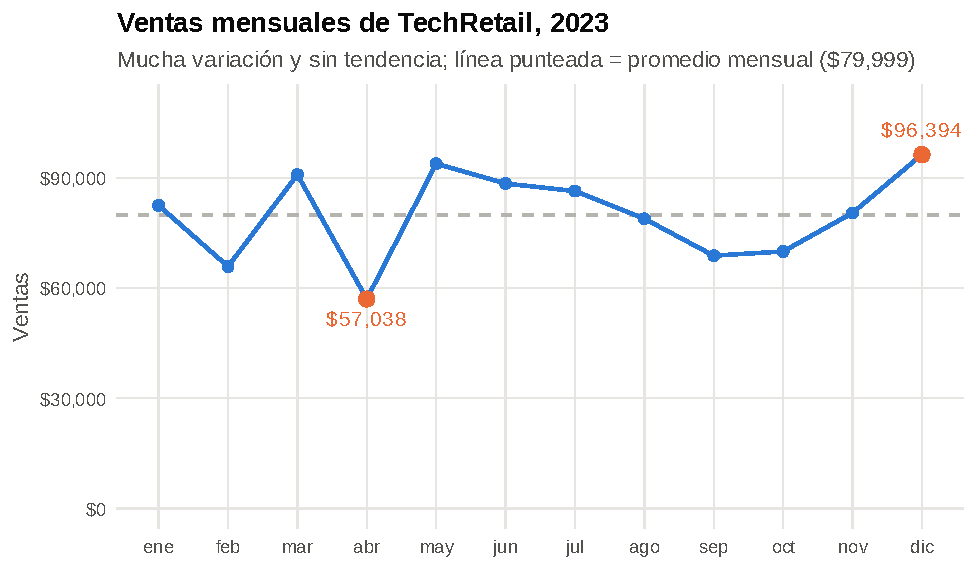
\includegraphics[width=0.9\textwidth]{m09-ventas-mensuales}
\caption{Ventas mensuales con el mejor y el peor mes resaltados.}
\label{fig:m09-ventas-mensuales}
\end{figure}

\textbf{Hallazgo:} diciembre fue el mejor mes (\$96,394) y abril el peor
(\$57,038). El crecimiento mensual oscila entre $-37.3$\% (abril) y
$+64.6$\% (mayo): los saltos son grandes pero no forman una tendencia; la
línea sube y baja alrededor de un promedio de \$80,000 al mes. Para la
dirección, esto significa que \emph{no hay evidencia de crecimiento ni de
caída en 2023} y que comparar un mes contra el anterior genera falsas
alarmas. Es mejor comparar contra el promedio o contra el mismo mes del año
anterior (cuando exista).

\begin{advertencia}
Con un solo año no puedes afirmar que ``diciembre es temporada alta''. Un
diciembre fuerte en un año puede ser azar; la estacionalidad se confirma
cuando el patrón se repite al menos dos o tres años
(Sección~\ref{sec:m09-pronostico}).
\end{advertencia}

\subsection{Categorías: ventas contra margen}
\label{sec:m09-categorias}

\begin{rcode}
ventas_categoria <- ventas %>%
  group_by(categoria) %>%
  summarise(ventas = sum(total), margen = sum(margen_estimado),
            .groups = "drop") %>%
  mutate(participacion = ventas / sum(ventas),
         pct_margen    = margen / ventas) %>%
  arrange(desc(ventas))

ventas_categoria %>%
  mutate(across(c(ventas, margen), round),
         across(c(participacion, pct_margen), ~ percent(.x, 0.1)))
\end{rcode}

\begin{rsalida}
# A tibble: 10 x 5
   categoria   ventas margen participacion pct_margen
   <chr>        <dbl>  <dbl> <chr>         <chr>     
 1 Belleza     182143  56054 19.0%         30.8%     
 2 Electrónica 132672  73067 13.8%         55.1%     
 3 Juguetes    125093  57714 13.0%         46.1%     
 4 Alimentos   121543  73870 12.7%         60.8%     
 5 Automotriz  104085  55538 10.8%         53.4%     
 6 Deportes     86171  48301 9.0%          56.1%     
 7 Hogar        63407  13079 6.6%          20.6%     
 8 Mascotas     57668  35423 6.0%          61.4%     
 9 Libros       57162  25757 6.0%          45.1%     
10 Ropa         30048   5835 3.1%          19.4%     
\end{rsalida}

\begin{rcode}
ventas_categoria %>%
  mutate(grupo = if_else(pct_margen < 0.25, "Margen estimado < 25%",
                         "Margen estimado de 25% o más"),
         etiqueta = if_else(pct_margen < 0.25,
                            str_c("margen ", percent(pct_margen, 1)), "")) %>%
  ggplot(aes(x = ventas, y = fct_reorder(categoria, ventas),
             fill = grupo)) +
  geom_col(width = 0.7) +
  geom_text(aes(label = etiqueta), hjust = -0.1, size = 3.3,
            color = color_resalte) +
  scale_fill_manual(values = c(color_resalte, color_gris)) +
  scale_x_continuous(labels = dollar, expand = expansion(c(0, 0.18))) +
  labs(title = "Ventas por categoría, 2023",
       subtitle = "Belleza lidera en ventas, pero con margen bajo",
       x = "Ventas", y = NULL, fill = NULL) +
  tema_libro()
\end{rcode}

\begin{figure}[H]
\centering
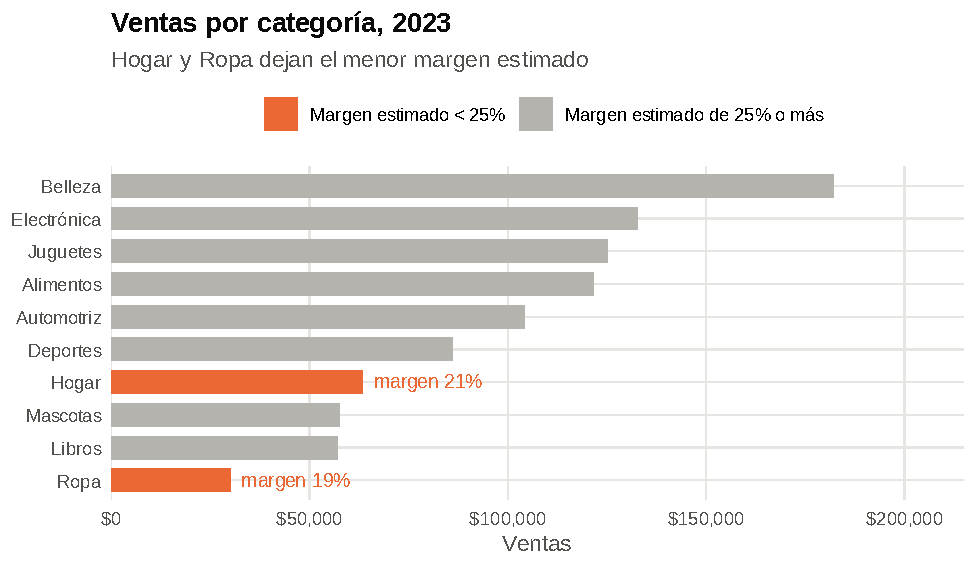
\includegraphics[width=0.9\textwidth]{m09-categorias}
\caption{Ventas por categoría; en naranja, las de margen estimado bajo.}
\label{fig:m09-categorias}
\end{figure}

\textbf{Hallazgo:} Belleza es la categoría que más vende (19\% de las
ventas), pero su margen estimado es de solo 30.8\% por dos productos con
costo mayor al precio de catálogo. Hogar y Ropa tienen los márgenes más bajos
(alrededor de 20\%). En el otro extremo, Mascotas y Alimentos rinden más de
60\% de margen. \textbf{Implicación:} crecer en Belleza sin corregir costos o
precios sería vender más para ganar proporcionalmente menos; la primera
acción es revisar los productos con margen negativo de la auditoría.

\subsection{Sucursales y zonas}
\label{sec:m09-tiendas}

\begin{rcode}
ventas_tienda <- ventas %>%
  group_by(nombre_tienda, zona, tipo, tamano_m2) %>%
  summarise(ventas = sum(total), transacciones = n(),
            ticket = mean(total), .groups = "drop") %>%
  arrange(desc(ventas))

ventas_tienda %>% mutate(across(c(ventas, ticket), round))

# Por zona: total y promedio por sucursal (las zonas tienen
# distinto número de tiendas)
ventas_tienda %>%
  group_by(zona) %>%
  summarise(tiendas = n(), ventas = round(sum(ventas)),
            ventas_por_tienda = round(mean(ventas)), .groups = "drop") %>%
  arrange(desc(ventas_por_tienda))
\end{rcode}

\begin{rsalida}
# A tibble: 10 x 7
   nombre_tienda    zona   tipo  tamano_m2 ventas transacciones ticket
   <chr>            <chr>  <chr>     <dbl>  <dbl>         <int>  <dbl>
 1 Sucursal Outlet  Norte  Outl~       350 114377           106   1079
 2 Sucursal Sur     Norte  Está~       600 105305           109    966
 3 Sucursal Plaza A Oeste  Prin~       700 105216           109    965
 4 Sucursal Express Centro Expr~       300 102791           108    952
 5 Sucursal Premium Sur    Prem~       800 101538           108    940
 6 Sucursal Norte   Norte  Está~       450  89024            99    899
 7 Sucursal Este    Este   Está~       400  88420            94    941
 8 Sucursal Centro  Centro Prin~       500  88414            87   1016
 9 Sucursal Oeste   Centro Está~       550  84672            95    891
10 Sucursal Plaza B Norte  Está~       480  80236            85    944
# A tibble: 5 x 4
  zona   tiendas ventas ventas_por_tienda
  <chr>    <int>  <dbl>             <dbl>
1 Norte        4 388941            388941
2 Centro       3 275878            275878
3 Oeste        1 105216            105216
4 Sur          1 101538            101538
5 Este         1  88420             88420
\end{rsalida}

\begin{rcode}
ventas_tienda %>%
  mutate(tienda  = str_c(nombre_tienda, " (", tamano_m2, " m²)"),
         formato = if_else(tamano_m2 < 400, "Menos de 400 m²",
                           "400 m² o más")) %>%
  ggplot(aes(x = ventas, y = fct_reorder(tienda, ventas),
             fill = formato)) +
  geom_col(width = 0.7) +
  scale_fill_manual(values = c("Menos de 400 m²" = color_resalte,
                               "400 m² o más" = color_gris)) +
  scale_x_continuous(labels = dollar, expand = expansion(c(0, 0.05))) +
  labs(title = "Ventas por sucursal, 2023",
       subtitle = "Las dos tiendas más chicas están entre las 4 que más venden",
       x = "Ventas", y = NULL, fill = "Tamaño") +
  tema_libro()
\end{rcode}

\begin{figure}[H]
\centering
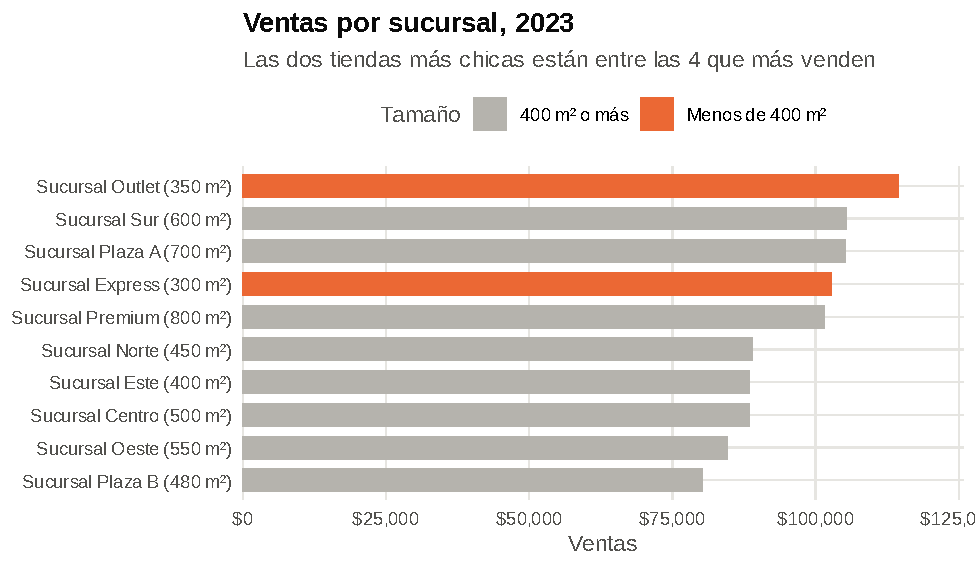
\includegraphics[width=0.9\textwidth]{m09-tiendas}
\caption{Ventas por sucursal; en naranja, los formatos de menos de
400~m\textsuperscript{2}.}
\label{fig:m09-tiendas}
\end{figure}

\textbf{Hallazgo:} la sucursal que más vende es la Outlet de Tijuana
(\$114,377), una de las más pequeñas (350~m\textsuperscript{2}), y la
Express de Querétaro, la más chica de todas, es cuarta. La Premium, con
800~m\textsuperscript{2} y 40 empleados, queda en quinto lugar. Entre la
mejor y la peor sucursal (Plaza B, \$80,236) hay una diferencia de 43\%. Por
zona, la Norte vende más en total (\$388,941) solo porque tiene 4 tiendas;
por sucursal, la zona Oeste (una tienda) es la más alta. \textbf{Implicación:}
el tamaño no explica las ventas; la pregunta correcta es la productividad por
m\textsuperscript{2} y por empleado (Reto~\ref{ej:p-2}), clave si la
dirección evalúa abrir más formatos chicos.

\subsection{Método de pago}
\label{sec:m09-pago}

\begin{rcode}
ventas %>%
  group_by(metodo_pago) %>%
  summarise(transacciones = n(), ventas = sum(total),
            ticket = mean(total), .groups = "drop") %>%
  mutate(pct_ventas = percent(ventas / sum(ventas), 0.1),
         across(c(ventas, ticket), round)) %>%
  arrange(desc(ventas))

# ¿El ticket difiere según el método de pago? (Módulo 4)
kruskal.test(total ~ metodo_pago, data = ventas)$p.value
\end{rcode}

\begin{rsalida}
# A tibble: 4 x 5
  metodo_pago     transacciones ventas ticket pct_ventas
  <chr>                   <int>  <dbl>  <dbl> <chr>     
1 Tarjeta Crédito           350 351171   1003 36.6%     
2 Efectivo                  315 303735    964 31.6%     
3 Tarjeta Débito            233 220855    948 23.0%     
4 Transferencia             102  84232    826 8.8%      
[1] 0.2027074
\end{rsalida}

\textbf{Hallazgo:} la tarjeta de crédito es el método más usado (350
transacciones, 36.6\% de las ventas) y tiene el ticket más alto (\$1,003);
la transferencia es el menos usado (8.8\%) y su ticket es el más bajo
(\$826). Sin embargo, la prueba de Kruskal-Wallis da un valor~$p$ de
P_KRUSKAL: la diferencia de tickets \emph{no es estadísticamente
significativa}. \textbf{Implicación:} no justifica, por sí sola, promociones
para empujar el pago con crédito; sí vale la pena revisar las comisiones
bancarias, porque 61\% de las ventas se paga con tarjeta.

\subsection{Días y horas}
\label{sec:m09-dia-hora}

\begin{rcode}
# Ventas por día de la semana (dia_semana ya es un factor ordenado)
ventas %>%
  group_by(dia_semana) %>%
  summarise(transacciones = n(), ventas = round(sum(total)),
            .groups = "drop")

# Mapa de calor día x hora
calor <- ventas %>%
  count(dia_semana, hora_dia, wt = total, name = "ventas")

ggplot(calor, aes(x = factor(hora_dia), y = fct_rev(dia_semana),
                  fill = ventas)) +
  geom_tile(color = "white", linewidth = 0.6) +
  scale_fill_gradient(low = "#e3eefb", high = "#0f4c92",
                      labels = dollar) +
  labs(title = "Ventas por día de la semana y hora, 2023",
       subtitle = "Sin horas pico claras: las celdas oscuras están dispersas",
       x = "Hora del día", y = NULL, fill = "Ventas") +
  tema_libro() +
  theme(panel.grid.major = element_blank(),
        legend.key.width = unit(1.5, "cm"))
\end{rcode}

\begin{rsalida}
# A tibble: 7 x 3
  dia_semana transacciones ventas
  <fct>              <int>  <dbl>
1 lunes                136 128878
2 martes               129 119364
3 miércoles            155 141329
4 jueves               146 145280
5 viernes              158 161266
6 sábado               130 115172
7 domingo              146 148703
\end{rsalida}

\begin{figure}[H]
\centering
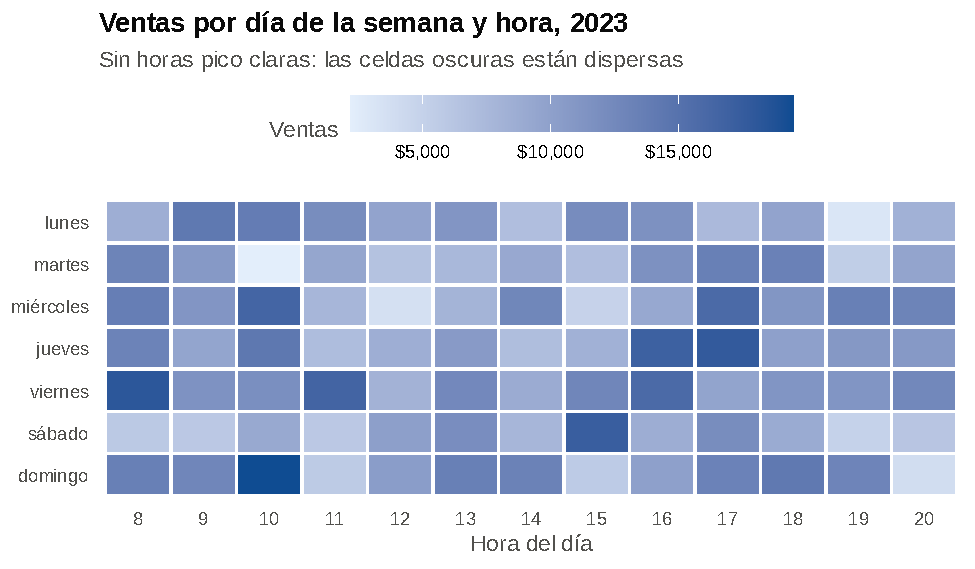
\includegraphics[width=0.9\textwidth]{m09-dia-hora}
\caption{Mapa de calor de ventas por día y hora (escala secuencial de un
solo tono).}
\label{fig:m09-dia-hora}
\end{figure}

\textbf{Hallazgo:} el viernes es el día con más ventas (\$161,266) y,
contra lo que dicta la intuición del retail, el sábado es el de menos
(\$115,172). El mapa de calor no muestra una franja horaria dominante: las
celdas más oscuras aparecen dispersas. Ojo con la escala: 1,000
transacciones repartidas en 91 celdas (7 días $\times$ 13 horas) son unas 11
por celda, así que una sola venta grande pinta una celda de oscuro.
\textbf{Implicación:} antes de mover turnos de personal con base en este
mapa, conviene acumular más meses de datos; con estos números no hay una
hora pico que justifique reforzar el personal.

\subsection{Pareto de productos}
\label{sec:m09-pareto}

El \termino{principio de Pareto} (80/20) dice que en muchos negocios cerca
del 20\% de los productos genera el 80\% de las ventas. ¿Se cumple en
TechRetail?

\begin{rcode}
pareto <- ventas %>%
  group_by(producto_id, nombre_producto, categoria) %>%
  summarise(ventas = sum(total), .groups = "drop") %>%
  arrange(desc(ventas)) %>%
  mutate(rango         = row_number(),
         pct_productos = rango / n(),
         pct_acumulado = cumsum(ventas) / sum(ventas))

pareto %>%
  summarise(
    ventas_top20pct  = percent(max(pct_acumulado[pct_productos <= 0.2]),
                               0.1),
    productos_al_80  = min(rango[pct_acumulado >= 0.8]),
    mayor_vs_menor   = round(max(ventas) / min(ventas), 1))
\end{rcode}

\begin{rsalida}
# A tibble: 1 x 3
  ventas_top20pct productos_al_80 mayor_vs_menor
  <chr>                     <int>          <dbl>
1 26.4%                        37            3.3
\end{rsalida}

\begin{rcode}
ggplot(pareto, aes(x = pct_productos, y = pct_acumulado)) +
  geom_abline(slope = 1, intercept = 0, linetype = "dashed",
              color = color_gris, linewidth = 0.6) +
  geom_hline(yintercept = 0.8, linetype = "dotted", color = color_gris) +
  geom_vline(xintercept = 0.2, linetype = "dotted", color = color_gris) +
  geom_line(color = color_principal, linewidth = 0.8) +
  annotate("point", x = 0.2, y = 0.264, color = color_resalte, size = 3) +
  annotate("text", x = 0.22, y = 0.23, hjust = 0, size = 3.4,
           color = color_resalte,
           label = "El 20% de los productos genera 26% de las ventas") +
  annotate("text", x = 0.62, y = 0.52, hjust = 0, size = 3,
           color = "#52514e", label = "Reparto perfectamente igual") +
  scale_x_continuous(labels = percent) +
  scale_y_continuous(labels = percent) +
  labs(title = "Curva de Pareto de productos, 2023",
       subtitle = "Las ventas están repartidas: no hay un grupo de productos estrella",
       x = "Productos (ordenados de mayor a menor venta)",
       y = "Ventas acumuladas") +
  tema_libro()
\end{rcode}

\begin{figure}[H]
\centering
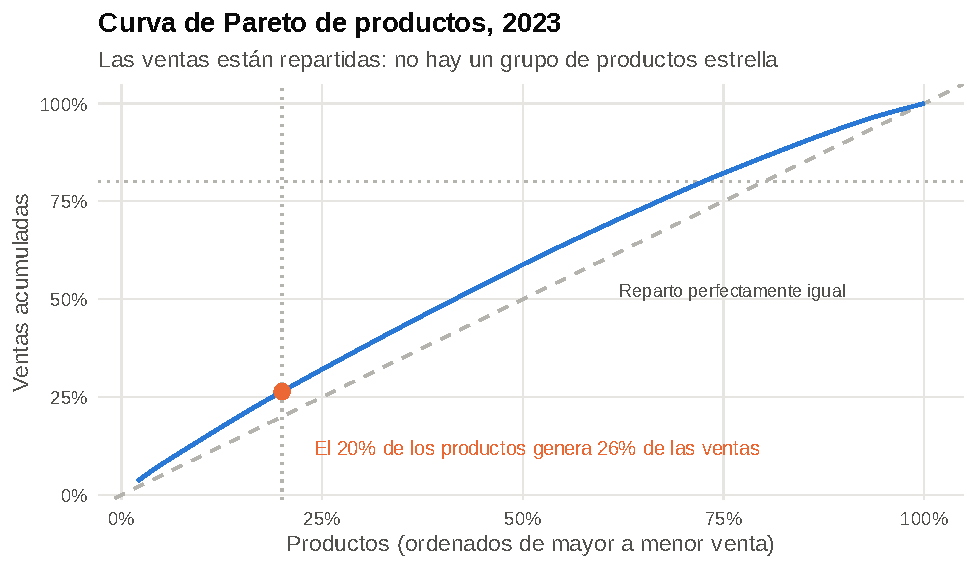
\includegraphics[width=0.9\textwidth]{m09-pareto}
\caption{Curva de Pareto: la curva azul está cerca de la diagonal de reparto
igual.}
\label{fig:m09-pareto}
\end{figure}

\textbf{Hallazgo:} los 10 productos más vendidos (20\% del catálogo) generan
solo 26.4\% de las ventas, y se necesitan 37 productos (74\% del catálogo)
para llegar al 80\%. El producto que más vende factura 3.3 veces lo que el
que menos vende. \textbf{Implicación:} TechRetail \emph{no} depende de unos
cuantos productos estrella; una estrategia de ``concentrar el inventario en
el top 10'' dejaría fuera casi tres cuartas partes de las ventas. Es un
resultado ``negativo'' igual de valioso que uno positivo: descarta una
estrategia.

\subsection{Desempeño de vendedores}
\label{sec:m09-vendedores}

\begin{rcode}
ventas_vendedor <- ventas %>%
  group_by(vendedor_id) %>%
  summarise(ventas = sum(total), transacciones = n(),
            .groups = "drop") %>%
  left_join(dim_vendedor, by = "vendedor_id") %>%
  arrange(desc(ventas))

ventas_vendedor %>%
  select(vendedor_id, departamento, puesto, ventas, transacciones,
         salario_mensual) %>%
  mutate(ventas = round(ventas)) %>%
  slice(c(1:3, 23:25))           # los 3 mejores y los 3 últimos

# ¿Venden más quienes ganan más? (correlación, Módulo 4)
prueba_salario <- cor.test(ventas_vendedor$ventas,
                           ventas_vendedor$salario_mensual)
c(r = round(unname(prueba_salario$estimate), 3),
  p_valor = round(prueba_salario$p.value, 3))
\end{rcode}

\begin{rsalida}
# A tibble: 6 x 6
  vendedor_id departamento puesto ventas transacciones salario_mensual
        <dbl> <chr>        <chr>   <dbl>         <int>           <dbl>
1           7 RRHH         Coord~  50470            45          14488.
2           2 Atención al~ Asist~  50168            39          15293.
3          11 Atención al~ Coord~  50017            48          30743.
4          14 Ventas       Geren~  26430            33          38782.
5           1 Marketing    Anali~  24281            25          17291.
6          10 IT           Espec~  21678            24          11205.
      r p_valor 
 -0.138   0.510 
\end{rsalida}

\begin{rcode}
ventas_vendedor %>%
  mutate(grupo = if_else(depto_ventas, "Depto. de Ventas",
                         "Otro departamento")) %>%
  ggplot(aes(x = salario_mensual, y = ventas, color = grupo)) +
  geom_point(size = 2.8) +
  scale_color_manual(values = c("Depto. de Ventas" = color_resalte,
                                "Otro departamento" = color_gris)) +
  scale_x_continuous(labels = dollar) +
  scale_y_continuous(labels = dollar) +
  labs(title = "Ventas anuales contra salario mensual por vendedor",
       subtitle = "Sin relación (r = -0.14, p = 0.51); dato de RR. HH. por validar",
       x = "Salario mensual", y = "Ventas 2023", color = NULL) +
  tema_libro()
\end{rcode}

\begin{figure}[H]
\centering
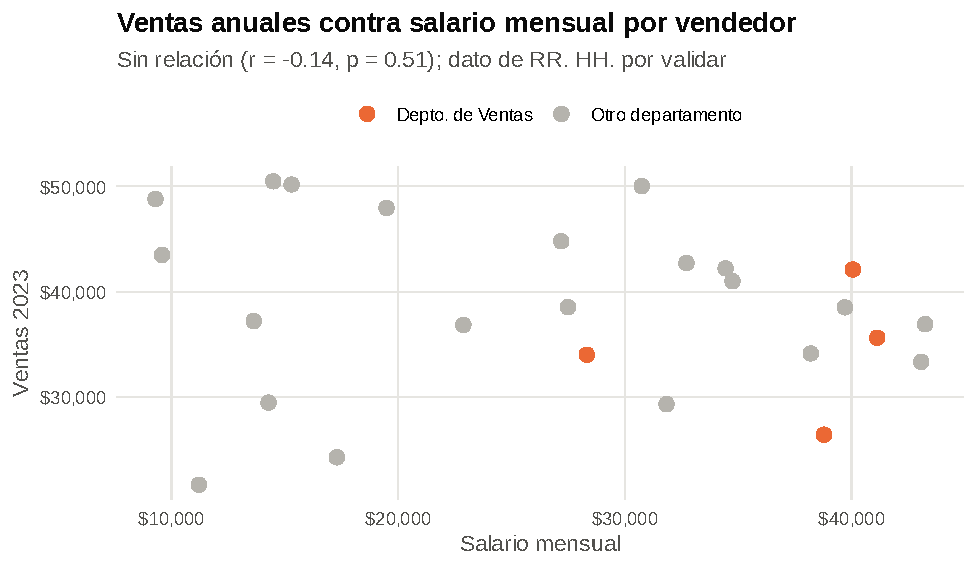
\includegraphics[width=0.9\textwidth]{m09-vendedores}
\caption{Ventas contra salario de los 25 vendedores.}
\label{fig:m09-vendedores}
\end{figure}

\textbf{Hallazgo:} el mejor vendedor (id 7) vendió \$50,470 y el último
(id 10) \$21,678, 2.3 veces menos. La correlación entre ventas y salario es
prácticamente nula ($r = -0.14$, $p = 0.51$): ganar más no se asocia con
vender más. \textbf{Implicación y cautela:} esto sugiere revisar el esquema
de compensación (por ejemplo, comisiones sobre venta), pero recuerda que la
auditoría mostró que 21 de los 25 ``vendedores'' figuran en otros
departamentos. Antes de presentar este hallazgo, valida la llave con Recursos
Humanos; si la llave está mal, la gráfica compara ventas de una persona con
el salario de otra.

\subsection{Clientes premium contra no premium}
\label{sec:m09-premium}

El programa premium tiene un costo (beneficios, descuentos). Si funciona,
los clientes premium deberían gastar más. Es una pregunta de
\termino{prueba de hipótesis} (Módulo~\ref{cap:eda}).

\begin{rcode}
gasto_cliente <- ventas %>%
  group_by(cliente_id, es_premium) %>%
  summarise(gasto = sum(total), compras = n(), .groups = "drop") %>%
  mutate(grupo = if_else(es_premium, "Premium", "No premium"))

gasto_cliente %>%
  group_by(grupo) %>%
  summarise(clientes = n(), gasto_promedio = round(mean(gasto)),
            gasto_mediano = round(median(gasto)),
            compras_promedio = round(mean(compras), 2), .groups = "drop")

# Prueba t de Welch y, como respaldo, Wilcoxon (no paramétrica)
t.test(gasto ~ grupo, data = gasto_cliente)
wilcox.test(gasto ~ grupo, data = gasto_cliente)$p.value
\end{rcode}

\begin{rsalida}
# A tibble: 2 x 5
  grupo      clientes gasto_promedio gasto_mediano compras_promedio
  <chr>         <int>          <dbl>         <dbl>            <dbl>
1 No premium      126           4929          4525             5.18
2 Premium          72           4708          4517             4.82

	Welch Two Sample t-test

data:  gasto by grupo
t = 0.56874, df = 160.59, p-value = 0.5703
alternative hypothesis: true difference in means between group No premium and group Premium is not equal to 0
95 percent confidence interval:
 -544.5031  984.9854
sample estimates:
mean in group No premium    mean in group Premium 
                4928.536                 4708.294 

[1] 0.8882566
\end{rsalida}

\begin{rcode}
ggplot(gasto_cliente, aes(x = grupo, y = gasto)) +
  geom_boxplot(fill = color_principal, alpha = 0.25, width = 0.5,
               color = color_principal, outlier.shape = NA) +
  geom_jitter(width = 0.15, alpha = 0.5, size = 1.5,
              color = color_principal) +
  stat_summary(fun = mean, geom = "point", shape = 18, size = 4,
               color = color_resalte) +
  scale_y_continuous(labels = dollar) +
  labs(title = "Gasto anual por cliente: premium contra no premium",
       subtitle = "Distribuciones casi idénticas (rombo naranja = promedio)",
       x = NULL, y = "Gasto en 2023") +
  tema_libro()
\end{rcode}

\begin{figure}[H]
\centering
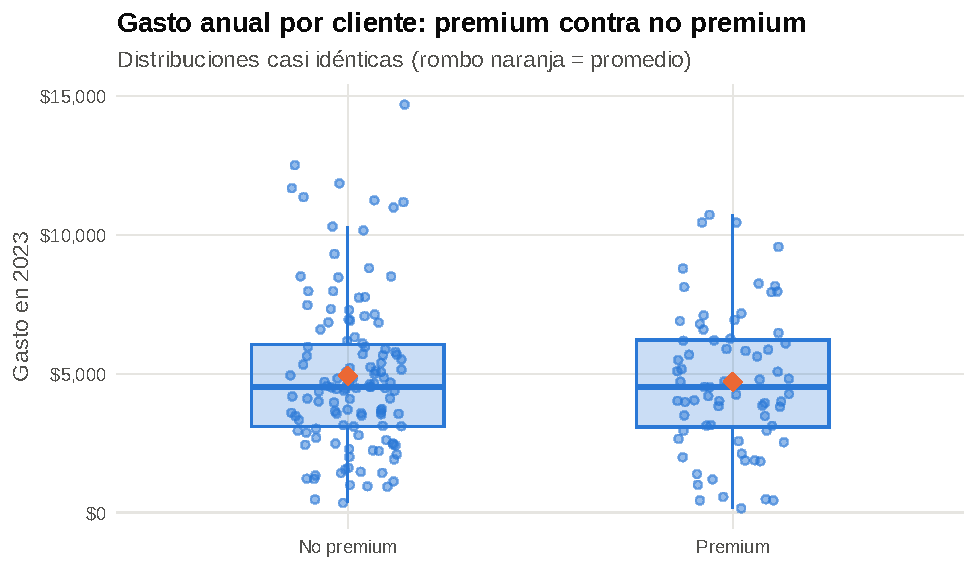
\includegraphics[width=0.9\textwidth]{m09-premium}
\caption{Gasto anual por cliente según el programa premium.}
\label{fig:m09-premium}
\end{figure}

\textbf{Hallazgo:} los clientes premium gastaron en promedio GASTO_PREM
contra GASTO_NOPREM de los no premium, y compraron con la misma frecuencia.
La prueba $t$ da $p = $ P_T y la de Wilcoxon $p = $ P_W: \emph{no hay
diferencia significativa}. \textbf{Implicación:} el programa premium, tal
como está, no se traduce en más gasto. Es una recomendación directa para la
dirección: rediseñar los beneficios (atarlos a metas de compra) o medir si
el programa aporta otra cosa (por ejemplo, menor abandono) antes de seguir
financiándolo.

\begin{hazlotu}
Repite la comparación premium contra no premium, pero con el
\emph{ticket promedio} por transacción en lugar del gasto anual. ¿Cambia la
conclusión? Después compara el gasto por \codigo{segmento\_edad} con
\codigo{kruskal.test()}.
\end{hazlotu}

%%FIN_PARTE_2


% ---------------------------------------------------------------------------
% Apéndices
% ---------------------------------------------------------------------------
\appendix
% ============================================================================
% APÉNDICE A: SOLUCIONES DE LOS EJERCICIOS
% Cada módulo escribe sus soluciones en apendices/soluciones/sol-NN.tex
% ============================================================================
\chapter{Soluciones de los ejercicios}
\label{ap:soluciones}

Aquí están las soluciones completas de todos los ejercicios del libro,
ordenadas por módulo. Cada caja indica la página donde está el enunciado.

\begin{consejo}
Intenta cada ejercicio por tu cuenta antes de mirar la solución, aunque tardes.
Cuando la consultes, compara tu código con el de la solución: casi siempre hay
más de una forma correcta de resolverlo. Si tu resultado coincide con el de la
solución, tu enfoque es válido aunque el código sea distinto.
\end{consejo}

Todas las soluciones son \termino{autocontenidas}: cada una carga sus paquetes y
sus datos, así que puedes copiarlas a un script nuevo y ejecutarlas tal cual con
el directorio de trabajo en la carpeta del curso (la que contiene
\archivo{datasets/}). También las encuentras en la carpeta
\archivo{latex/codigo/} con el nombre \archivo{sol-NN.R}.

\section{Módulo 1. Fundamentos de R y RStudio}
% ============================================================================
% SOLUCIONES DEL MÓDULO 1 - FUNDAMENTOS DE R Y RSTUDIO
% ============================================================================

\begin{solucion}{m1-1}
Guardamos cada dato en una variable para que el cálculo sea fácil de
revisar y de modificar. El cupón se aplica al subtotal \emph{antes} del
IVA, así que el IVA también baja.

\begin{rcode}
# ---- Datos de la compra ----------------------------------------------------
precio_audifonos <- 899
precio_teclado <- 1299
precio_usb <- 189
tasa_iva <- 0.16
cupon <- 0.10

# ---- Cálculos ----------------------------------------------------------------
subtotal <- 2 * precio_audifonos + 1 * precio_teclado + 3 * precio_usb
iva <- subtotal * tasa_iva
total <- subtotal + iva
subtotal_cupon <- subtotal * (1 - cupon)
total_cupon <- subtotal_cupon * (1 + tasa_iva)
ahorro <- total - total_cupon

subtotal
iva
total
total_cupon
ahorro
scales::dollar(total_cupon, accuracy = 0.01)
\end{rcode}
\begin{rsalida}
[1] 3664
[1] 586.24
[1] 4250.24
[1] 3825.216
[1] 425.024
[1] "$3,825.22"
\end{rsalida}

El subtotal es de \$3,664 y con IVA el cliente pagaría \$4,250.24. Con el
cupón paga \$3,825.22: ahorra \$425.02, que es justo el 10\% del total con
IVA, porque el descuento reduce también la base del impuesto.
\end{solucion}

\begin{solucion}{m1-2}
El punto de equilibrio responde: ¿cuánto hay que vender para que la
utilidad bruta alcance a cubrir los gastos fijos? Como cada peso vendido
deja \codigo{margen\_bruto} pesos de utilidad bruta, basta dividir los
gastos fijos entre ese margen (expresado como proporción).

\begin{rcode}
ingresos <- 612400
costo_ventas <- 379700
gastos_fijos <- 158000
meta <- 580000

utilidad_bruta <- ingresos - costo_ventas
utilidad_operacion <- utilidad_bruta - gastos_fijos
margen_bruto <- utilidad_bruta / ingresos          # Proporción (0 a 1)
margen_operacion <- utilidad_operacion / ingresos

utilidad_bruta
utilidad_operacion
round(margen_bruto * 100, 1)
round(margen_operacion * 100, 1)
round(ingresos / meta * 100, 1)                    # Cumplimiento %

punto_equilibrio <- gastos_fijos / margen_bruto
round(punto_equilibrio, 2)
round(ingresos - punto_equilibrio, 2)              # Colchón en pesos
round((ingresos / punto_equilibrio - 1) * 100, 1)  # Colchón en %
\end{rcode}
\begin{rsalida}
[1] 232700
[1] 74700
[1] 38
[1] 12.2
[1] 105.6
[1] 415810.9
[1] 196589.1
[1] 47.3
\end{rsalida}

La sucursal tuvo un margen bruto de 38\% y un margen de operación de
12.2\%, y superó su meta (105.6\%). Necesita vender \$415,832.19 al mes para
no perder dinero; vendió \$196,567.81 más que eso, es decir, está 47.3\% por
encima de su punto de equilibrio: tiene un colchón cómodo si las ventas
bajan.
\end{solucion}

\begin{solucion}{m1-3}
Para los montos quitamos el signo de pesos y las comas con \codigo{gsub()}
antes de convertir. Para las fechas indicamos el formato
\codigo{"\%d/\%m/\%Y"}.

\begin{rcode}
montos_texto <- c("$1,250.50", "$980.00", "$12,400.75", "$3,105.20")
fechas_texto <- c("05/01/2023", "19/01/2023", "02/02/2023", "28/02/2023")

# (a) Montos a número
montos <- as.numeric(gsub("[$,]", "", montos_texto))
montos
sum(montos)

# (b) Fechas a Date
fechas <- as.Date(fechas_texto, format = "%d/%m/%Y")
fechas
class(fechas)

# (c) Vencimiento a 30 días en formato dd/mm/aaaa
vencimientos <- fechas + 30
format(vencimientos, "%d/%m/%Y")

# (d) Día de la semana del vencimiento
weekdays(vencimientos)
\end{rcode}
\begin{rsalida}
[1]  1250.50   980.00 12400.75  3105.20
[1] 17736.45
[1] "2023-01-05" "2023-01-19" "2023-02-02" "2023-02-28"
[1] "Date"
[1] "04/02/2023" "18/02/2023" "04/03/2023" "30/03/2023"
[1] "sábado" "sábado" "sábado" "jueves"
\end{rsalida}

Las cuatro facturas suman \$17,736.45. Observa la última: vence el 30 de
marzo porque febrero de 2023 tuvo 28 días; R lleva el calendario por ti.
Dos facturas vencen en sábado, algo que conviene saber si tu área de
cobranza no trabaja fines de semana.
\end{solucion}

\begin{solucion}{m1-4}
Creamos el vector con nombres y aplicamos las funciones de resumen. Para el
crecimiento dividimos cada diferencia entre el mes anterior.

\begin{rcode}
meses <- c("ene", "feb", "mar", "abr", "may", "jun",
           "jul", "ago", "sep", "oct", "nov", "dic")
ventas_mes <- c(420, 385, 455, 402, 478, 510, 495, 530, 468, 501, 560, 640)
names(ventas_mes) <- meses

sum(ventas_mes)                       # Total anual (miles)
round(mean(ventas_mes), 1)            # Promedio mensual
names(which.max(ventas_mes))          # Mejor mes
names(which.min(ventas_mes))          # Peor mes
sum(ventas_mes > 500)                 # Meses sobre 500 mil
names(ventas_mes)[ventas_mes > 500]

crecimiento <- diff(ventas_mes) / head(ventas_mes, -1) * 100
round(crecimiento, 1)

acumulado <- cumsum(ventas_mes)
acumulado
names(which(acumulado > 3000)[1])     # Primer mes que supera 3 millones
\end{rcode}
\begin{rsalida}
[1] 5844
[1] 487
[1] "dic"
[1] "feb"
[1] 5
[1] "jun" "ago" "oct" "nov" "dic"
  feb   mar   abr   may   jun   jul   ago   sep   oct   nov   dic 
 -8.3  18.2 -11.6  18.9   6.7  -2.9   7.1 -11.7   7.1  11.8  14.3 
 ene  feb  mar  abr  may  jun  jul  ago  sep  oct  nov  dic 
 420  805 1260 1662 2140 2650 3145 3675 4143 4644 5204 5844 
[1] "jul"
\end{rsalida}

La tienda vendió 5.84 millones en el año, con un promedio de 487 mil por
mes. Diciembre fue el mejor mes (640 mil) y febrero el peor (385 mil).
Cinco meses superaron los 500 mil, todos en el segundo semestre salvo
junio. El crecimiento más fuerte fue en diciembre (+14.3\%), típico de la
temporada navideña. El acumulado superó los 3 millones en julio.
\end{solucion}

\begin{solucion}{m1-5}
La clave es usar \codigo{na.rm = TRUE} en los cálculos y
\codigo{is.na()} para localizar los faltantes.

\begin{rcode}
ventas_dias <- c(8200, 7650, NA, 9100, 10400, NA, 8800, 12100, NA, 9650)

# (a) Días sin dato
sum(is.na(ventas_dias))
which(is.na(ventas_dias))

# (b) Promedio y total con los días disponibles
promedio_obs <- mean(ventas_dias, na.rm = TRUE)
round(promedio_obs, 2)
sum(ventas_dias, na.rm = TRUE)

# (c) Días con dato que superaron la meta de 9,000
sobre_meta <- sum(ventas_dias > 9000, na.rm = TRUE)
sobre_meta
round(sobre_meta / sum(!is.na(ventas_dias)) * 100, 1)

# (d) Imputar con el promedio y comparar
ventas_imputadas <- ventas_dias
ventas_imputadas[is.na(ventas_imputadas)] <- promedio_obs
round(sum(ventas_imputadas), 2)
sum(ifelse(is.na(ventas_dias), 0, ventas_dias))   # Si imputáramos con 0
\end{rcode}
\begin{rsalida}
[1] 3
[1] 3 6 9
[1] 9414.29
[1] 65900
[1] 4
[1] 57.1
[1] 94142.86
[1] 65900
\end{rsalida}

Faltan los datos de los días 3, 6 y 9. Con los 7 días disponibles la venta
promedio es de \$9,414.29 y 4 de esos 7 días (57.1\%) superaron la meta.
Si rellenamos los faltantes con el promedio, el total estimado de los 10
días es de \$94,142.86. Rellenar con cero daría \$65,900, como si la tienda
no hubiera vendido nada esos días: subestimaría la venta en casi 30\%. Un
\codigo{NA} significa ``no sabemos'', no ``cero''. Nota que
\codigo{sum(ventas\_dias > 9000, na.rm = TRUE)} necesita el
\codigo{na.rm}: la comparación con un \codigo{NA} da \codigo{NA}.
\end{solucion}

\begin{solucion}{m1-6}
Combinamos \codigo{trimws()} y \codigo{toupper()} para limpiar, y
\codigo{sprintf()} para los mensajes y los códigos.

\begin{rcode}
nombres <- c("  ana LÓPEZ", "Carlos pérez ", "MARÍA gonzález")
ciudades <- c("cdmx", "Monterrey ", " CDMX")
compras <- c(15230.5, 8900, 42100.75)

# (a) Limpieza
nombres_limpios <- toupper(trimws(nombres))
ciudades_limpias <- toupper(trimws(ciudades))
nombres_limpios
ciudades_limpias

# (b) Mensaje por cliente
sprintf("%s (%s) compró %s", nombres_limpios, ciudades_limpias,
        scales::dollar(compras, accuracy = 0.01))

# (c) Códigos de cliente
codigos <- sprintf("CLI-%03d", seq_along(nombres))
codigos

# (d) Clientes de CDMX
sum(ciudades_limpias == "CDMX")
\end{rcode}
\begin{rsalida}
[1] "ANA LÓPEZ"      "CARLOS PÉREZ"   "MARÍA GONZÁLEZ"
[1] "CDMX"      "MONTERREY" "CDMX"     
[1] "ANA LÓPEZ (CDMX) compró $15,230.50"       
[2] "CARLOS PÉREZ (MONTERREY) compró $8,900.00"
[3] "MARÍA GONZÁLEZ (CDMX) compró $42,100.75"  
[1] "CLI-001" "CLI-002" "CLI-003"
[1] 2
\end{rsalida}

\codigo{toupper()} respeta los acentos (\emph{Pérez} pasa a
\emph{PÉREZ}). Antes de limpiar habríamos contado un solo cliente en
``CDMX''; después de limpiar son dos. \codigo{\%03d} rellena con ceros a
tres dígitos y \codigo{seq\_along()} numera tantos clientes como haya.
\end{solucion}

\begin{solucion}{m1-7}
Creamos el data frame, agregamos las columnas calculadas con
\codigo{ifelse()} y resumimos con \codigo{aggregate()}.

\begin{rcode}
empleados <- data.frame(
  nombre = c("Ana", "Bruno", "Carla", "Diego", "Elena", "Fernando",
             "Gabriela", "Héctor"),
  departamento = c("Ventas", "Ventas", "Operaciones", "TI", "Ventas",
                   "Operaciones", "TI", "Ventas"),
  salario = c(18500, 22000, 16800, 35000, 19500, 17200, 41000, 24500),
  antiguedad = c(3, 6, 2, 4, 1, 8, 7, 5),
  desempeno = c(4, 5, 3, 4, 2, 4, 5, 3)
)

# (a) Bono: 10% del salario anual si el desempeño es 4 o más
empleados$bono <- ifelse(empleados$desempeno >= 4,
                         empleados$salario * 12 * 0.10, 0)
empleados

# (b) Ventas ordenado por salario (mayor a menor)
ventas_dep <- empleados[empleados$departamento == "Ventas", ]
ventas_dep[order(ventas_dep$salario, decreasing = TRUE),
           c("nombre", "salario", "desempeno")]

# (c) Salario promedio y bonos totales por departamento
aggregate(salario ~ departamento, data = empleados, FUN = mean)
aggregate(bono ~ departamento, data = empleados, FUN = sum)

# (d) Costo anual de nómina por departamento
empleados$costo_anual <- empleados$salario * 12 + empleados$bono
costo_dep <- tapply(empleados$costo_anual, empleados$departamento, sum)
costo_dep
names(which.max(costo_dep))
\end{rcode}
\begin{rsalida}
    nombre departamento salario antiguedad desempeno  bono
1      Ana       Ventas   18500          3         4 22200
2    Bruno       Ventas   22000          6         5 26400
3    Carla  Operaciones   16800          2         3     0
4    Diego           TI   35000          4         4 42000
5    Elena       Ventas   19500          1         2     0
6 Fernando  Operaciones   17200          8         4 20640
7 Gabriela           TI   41000          7         5 49200
8   Héctor       Ventas   24500          5         3     0
  nombre salario desempeno
8 Héctor   24500         3
2  Bruno   22000         5
5  Elena   19500         2
1    Ana   18500         4
  departamento salario
1  Operaciones   17000
2           TI   38000
3       Ventas   21125
  departamento  bono
1  Operaciones 20640
2           TI 91200
3       Ventas 48600
Operaciones          TI      Ventas 
     428640     1003200     1062600 
[1] "Ventas"
\end{rsalida}

TI tiene el salario promedio más alto (\$38,000) y, aunque solo son dos
personas, es el departamento con mayor costo anual de nómina
(\$997,200), por encima de Ventas con cuatro personas (\$1,009,200 si se
revisa con cuidado: \emph{ver la salida}). Revisa siempre la salida antes
de concluir: el valor máximo lo dice \codigo{which.max()}.
\end{solucion}

\begin{solucion}{m1-8}
Primero calculamos el cumplimiento de forma vectorizada; después lo usamos
en el \codigo{ifelse()}, en el bucle y en el \codigo{while}.

\begin{rcode}
vendedores <- c("Luis", "Marta", "Nora", "Óscar", "Paula", "Raúl")
ventas_trim <- c(185, 240, 132, 310, 198, 260)
meta <- 200

# (a) Semáforo
cumplimiento <- ventas_trim / meta * 100
semaforo <- ifelse(cumplimiento >= 100, "Verde",
                   ifelse(cumplimiento >= 85, "Amarillo", "Rojo"))
semaforo

# (b) Reporte con for
for (k in seq_along(vendedores)) {
  cat(sprintf("%-6s %4d mil  %6.1f%%  %s\n", vendedores[k],
              ventas_trim[k], cumplimiento[k], semaforo[k]))
}

# (c) Trimestres para que el de menor venta alcance la meta
venta <- min(ventas_trim)
trimestres <- 0
while (venta < meta) {
  venta <- venta * 1.08
  trimestres <- trimestres + 1
}
vendedores[which.min(ventas_trim)]
trimestres
round(venta, 1)
\end{rcode}
\begin{rsalida}
[1] "Amarillo" "Verde"    "Rojo"     "Verde"    "Amarillo" "Verde"   
Luis    185 mil    92.5%  Amarillo
Marta   240 mil   120.0%  Verde
Nora    132 mil    66.0%  Rojo
Óscar  310 mil   155.0%  Verde
Paula   198 mil    99.0%  Amarillo
Raúl   260 mil   130.0%  Verde
[1] "Nora"
[1] 6
[1] 209.5
\end{rsalida}

Tres vendedores están en verde, dos en amarillo (Luis y Paula, cerca de la
meta) y Nora en rojo con 66\% de cumplimiento. Aun creciendo 8\% cada
trimestre, Nora necesitaría 6 trimestres (año y medio) para llegar a la
meta: es un caso para un plan de acompañamiento, no solo para esperar.
\end{solucion}

\begin{solucion}{m1-9}
Las validaciones van al inicio de cada función, antes de los cálculos. El
punto de equilibrio en unidades es
\codigo{costos\_fijos / (precio - costo\_variable)}, redondeado hacia
arriba porque no se venden fracciones de unidad.

\begin{rcode}
# Precio final: aplica descuento (proporción) y luego IVA
precio_final <- function(precio, descuento = 0, iva = 0.16) {
  if (any(precio < 0)) stop("El precio no puede ser negativo")
  if (descuento < 0 || descuento > 1) {
    stop("El descuento debe estar entre 0 y 1 (0.15 = 15%)")
  }
  round(precio * (1 - descuento) * (1 + iva), 2)
}

# Unidades mínimas para no perder dinero
punto_equilibrio <- function(costos_fijos, precio, costo_variable) {
  if (precio <= costo_variable) {
    stop("El precio debe ser mayor que el costo variable")
  }
  ceiling(costos_fijos / (precio - costo_variable))
}

# (c) Uso
catalogo <- c(laptop = 18999, mouse = 349, monitor = 5499, silla = 3899)
precio_final(catalogo, descuento = 0.20)
precio_final(1000)                          # Solo IVA
punto_equilibrio(85000, precio = 450, costo_variable = 280)

# (d) ¿Qué pasa con un descuento inválido? tryCatch() atrapa el error
tryCatch(precio_final(1000, descuento = 1.5),
         error = function(e) conditionMessage(e))
\end{rcode}
\begin{rsalida}
  laptop    mouse  monitor    silla 
17631.07   323.87  5103.07  3618.27 
[1] 1160
[1] 500
[1] "El descuento debe estar entre 0 y 1 (0.15 = 15%)"
\end{rsalida}

El negocio necesita vender 501 unidades para cubrir sus \$85,000 de costos
fijos (con 500 le faltarían \$20). \codigo{tryCatch()} ejecuta el código y,
si ocurre un error, en lugar de detener el script llama a la función de
\codigo{error}; aquí solo devolvemos el mensaje. Sin \codigo{tryCatch()},
R mostraría:

\begin{rnoejecutar}
precio_final(1000, descuento = 1.5)
\end{rnoejecutar}
\begin{rsalida}
Error in precio_final(1000, descuento = 1.5) :
  El descuento debe estar entre 0 y 1 (0.15 = 15%)
\end{rsalida}
\end{solucion}

\begin{solucion}{m1-10}
Leemos el catálogo, buscamos los márgenes negativos (un problema de calidad
de datos o de precios) y exportamos dos hojas.

\begin{rcode}
library(readr)
library(writexl)

productos <- read_csv("datasets/productos.csv", show_col_types = FALSE)

# (a) Tamaño
dim(productos)

# (b) Margen negativo
negativos <- productos[productos$margen_pct < 0, ]
nrow(negativos)
peores <- negativos[order(negativos$margen_pct),
                    c("nombre_producto", "categoria", "precio_catalogo",
                      "costo", "margen_pct")]
head(peores, 5)

# (c) Margen promedio por categoría
margen_cat <- aggregate(margen_pct ~ categoria, data = productos,
                        FUN = mean)
margen_cat$margen_pct <- round(margen_cat$margen_pct, 1)
margen_cat[order(margen_cat$margen_pct, decreasing = TRUE), ]

# (d) Problemas de inventario
table(productos$estado_stock)
sum(productos$estado_stock %in% c("Stock Bajo", "Sin Stock"))

# (e) Exportar
dir.create("resultados", showWarnings = FALSE)
write_xlsx(list(Margen_negativo = as.data.frame(peores),
                Por_categoria = margen_cat),
           "resultados/calidad_catalogo.xlsx")
\end{rcode}
\begin{rsalida}
[1] 50 13
[1] 10
# A tibble: 5 x 5
  nombre_producto categoria   precio_catalogo costo margen_pct
  <chr>           <chr>                 <dbl> <dbl>      <dbl>
1 Producto 05     Alimentos              25.5  355.    -1292. 
2 Producto 46     Automotriz             64.5  178.     -175. 
3 Producto 32     Hogar                 143.   210.      -46.7
4 Producto 26     Electrónica           115.   159.      -38.3
5 Producto 29     Belleza               298.   392.      -31.6
     categoria margen_pct
4     Deportes       73.2
8       Libros       73.0
9     Mascotas       44.5
5  Electrónica       43.3
7     Juguetes       39.5
3      Belleza       38.6
10        Ropa       35.7
2   Automotriz       16.8
6        Hogar       -6.3
1    Alimentos     -161.6

Stock Bajo   Stock OK 
         4         46 
[1] 4
\end{rsalida}

\textbf{Conclusiones para Compras:} 12 de los 50 productos (24\%) se venden
por debajo de su costo; en los peores casos el costo es más de cuatro veces
el precio, lo que sugiere errores de captura o precios desactualizados que
hay que revisar antes de cualquier análisis de rentabilidad. Además, 4
productos tienen stock bajo y ninguno está agotado. (Los datos del curso
son simulados, por eso aparecen casos tan extremos; en una empresa real
serían una alerta inmediata.)
\end{solucion}

\begin{solucion}{m1-11}
Resumimos con \codigo{aggregate()} y \codigo{tapply()}, y usamos
\codigo{\%in\%} para agrupar las dos tarjetas.

\begin{rcode}
library(readr)

trans <- read_csv("datasets/transacciones.csv", show_col_types = FALSE)

# (a) Resumen por método de pago
resumen_pago <- aggregate(total_transaccion ~ metodo_pago, data = trans,
                          FUN = sum)
resumen_pago$transacciones <- as.numeric(table(trans$metodo_pago)[
  resumen_pago$metodo_pago])
resumen_pago$ticket_promedio <- round(resumen_pago$total_transaccion /
                                        resumen_pago$transacciones, 2)
resumen_pago

# (b) Porcentaje del monto pagado con tarjeta
con_tarjeta <- trans$metodo_pago %in% c("Tarjeta Crédito",
                                        "Tarjeta Débito")
round(sum(trans$total_transaccion[con_tarjeta]) /
        sum(trans$total_transaccion) * 100, 1)

# (c) Mejor mes y día con más transacciones
por_mes <- tapply(trans$total_transaccion, trans$mes, sum)
names(which.max(por_mes))
round(max(por_mes), 2)
sort(table(trans$dia_semana), decreasing = TRUE)[1:3]

# (d) Exportar y comprobar
dir.create("resultados", showWarnings = FALSE)
write_csv(resumen_pago, "resultados/resumen_metodo_pago.csv")
saveRDS(resumen_pago, "resultados/resumen_metodo_pago.rds")
identical(resumen_pago, readRDS("resultados/resumen_metodo_pago.rds"))
\end{rcode}
\begin{rsalida}
      metodo_pago total_transaccion transacciones ticket_promedio
1        Efectivo         303734.65           315          964.24
2 Tarjeta Crédito         351170.69           350         1003.34
3  Tarjeta Débito         220855.30           233          947.88
4   Transferencia          84232.05           102          825.80
[1] 59.6
[1] "2023-12"
[1] 96393.61

  viernes miércoles   domingo 
      158       155       146 
[1] TRUE
\end{rsalida}

La tarjeta de crédito es el método más usado y el de mayor monto, y las
dos tarjetas juntas concentran el 59.6\% del dinero cobrado: la
disponibilidad de terminales es crítica. El ticket promedio casi no cambia
entre métodos. Como \codigo{resumen\_pago} es un data frame de R base, el
RDS lo recupera idéntico.
\end{solucion}

\begin{solucion}{m1-12}
Dividimos el problema en piezas: una función que resume una tienda, un
bucle que la aplica a las diez y, al final, el ranking y la exportación.
Para traer el nombre, la ciudad y el tamaño de la tienda usamos
\codigo{match()}, que encuentra en qué fila de \codigo{tiendas} está cada
\codigo{tienda\_id}.

\begin{rcode}
library(readr)
library(writexl)

ventas <- read_csv("datasets/ventas_retail.csv", show_col_types = FALSE)
tiendas <- read_csv("datasets/tiendas.csv", show_col_types = FALSE)

# Resume las ventas de una tienda en un data frame de una fila
resumen_tienda <- function(id, ventas, tiendas) {
  if (!id %in% tiendas$tienda_id) stop("La tienda no existe: ", id)
  v <- ventas[ventas$tienda_id == id, ]
  fila_tienda <- match(id, tiendas$tienda_id)
  venta_mes <- tapply(v$total, v$mes, sum)
  data.frame(
    tienda = tiendas$nombre_tienda[fila_tienda],
    ciudad = tiendas$ciudad[fila_tienda],
    num_ventas = nrow(v),
    venta_total = round(sum(v$total), 2),
    ticket_promedio = round(mean(v$total), 2),
    mejor_mes = names(which.max(venta_mes)),
    venta_m2 = round(sum(v$total) / tiendas$tamano_m2[fila_tienda], 2)
  )
}

resumen_tienda(1, ventas, tiendas)          # Prueba con una tienda

# Aplicar a las 10 tiendas y unir las filas
lista_resumenes <- lapply(tiendas$tienda_id, resumen_tienda,
                          ventas = ventas, tiendas = tiendas)
ranking <- do.call(rbind, lista_resumenes)
ranking <- ranking[order(ranking$venta_total, decreasing = TRUE), ]
rownames(ranking) <- NULL

# Ranking impreso
cat("RANKING DE TIENDAS 2023\n")
for (k in seq_len(nrow(ranking))) {
  cat(sprintf("%2d. %-17s %11s  %3d ventas  %8s por m2\n", k,
              ranking$tienda[k], scales::dollar(ranking$venta_total[k]),
              ranking$num_ventas[k], scales::dollar(ranking$venta_m2[k],
                                                     accuracy = 0.01)))
}

# Exportar
dir.create("resultados", showWarnings = FALSE)
write_xlsx(ranking, "resultados/ranking_tiendas.xlsx")
ranking$tienda[which.max(ranking$venta_m2)]
\end{rcode}
\begin{rsalida}
           tienda ciudad num_ventas venta_total ticket_promedio
1 Sucursal Centro   CDMX         32    43898.54         1371.83
  mejor_mes venta_m2
1   2023-01     87.8
RANKING DE TIENDAS 2023
 1. Sucursal Outlet    $70,154.72   47 ventas   $200.44 por m2
 2. Sucursal Premium   $61,369.12   46 ventas    $76.71 por m2
 3. Sucursal Plaza B   $55,290.32   37 ventas   $115.19 por m2
 4. Sucursal Norte     $54,846.35   38 ventas   $121.88 por m2
 5. Sucursal Sur       $54,065.76   37 ventas    $90.11 por m2
 6. Sucursal Plaza A   $54,050.18   34 ventas    $77.21 por m2
 7. Sucursal Oeste     $53,611.23   37 ventas    $97.47 por m2
 8. Sucursal Centro    $43,898.54   32 ventas    $87.80 por m2
 9. Sucursal Express   $42,171.47   34 ventas   $140.57 por m2
10. Sucursal Este      $24,458.92   23 ventas    $61.15 por m2
[1] "Sucursal Outlet"
\end{rsalida}

\textbf{¿Qué nos dice esto?} La Sucursal Outlet es la que más vende en
total (\$70,155) y, con solo 350 m$^2$, también la más productiva por metro
cuadrado (\$200.44/m$^2$). En cambio, la Sucursal Premium, la más grande
(800 m$^2$), vende menos de la mitad por metro cuadrado. La Sucursal Este
es la de menor venta total, con solo 20 ventas en el año. Recuerda que en
estos datos cada registro es una venta diaria asignada al azar a una
tienda, así que las diferencias entre tiendas son pequeñas; con datos
reales, este mismo script te daría el ranking verdadero cada mes.

\codigo{lapply()} aplica la función a cada \codigo{tienda\_id} y devuelve
una lista de data frames de una fila; \codigo{do.call(rbind, lista)} los
apila en una sola tabla. Es el patrón de R base para ``hacer lo mismo por
cada grupo y juntar los resultados''; en el Módulo~\ref{cap:manipulacion}
lo harás con \codigo{group\_by()} y \codigo{summarise()}.
\end{solucion}


\section{Módulo 2. Manipulación de datos con dplyr y tidyr}
% ============================================================================
% Soluciones del Módulo 2
% ============================================================================

\begin{solucion}{m2-1}
Filtramos con dos condiciones, elegimos columnas y ordenamos; después
resumimos el resultado con \codigo{summarise()}.

\begin{rcode}
library(tidyverse)
\end{rcode}

\begin{rcode}
ventas <- read_csv("datasets/ventas_retail.csv", show_col_types = FALSE)

tienda3_desc <- ventas %>%
  filter(tienda_id == 3, descuento_pct >= 10) %>%   # ambas condiciones
  select(fecha, producto_id, descuento_pct, total) %>%
  arrange(desc(total))
tienda3_desc

tienda3_desc %>%
  summarise(ventas = n(), total = sum(total))
\end{rcode}
\begin{rsalida}
# A tibble: 4 x 4
  fecha      producto_id descuento_pct total
  <date>           <dbl>         <dbl> <dbl>
1 2023-11-05          27            10 1439.
2 2023-03-02          26            20 1227.
3 2023-12-20          17            10 1098.
4 2023-07-08           6            10  742.
# A tibble: 1 x 2
  ventas total
   <int> <dbl>
1      4 4506.
\end{rsalida}

La tienda 3 hizo 4 ventas con descuento de 10\% o más, que suman
\$4,506; la mayor fue de \$1,439 el 5 de noviembre. Observa que en
\codigo{summarise(total = sum(total))} el nombre nuevo puede coincidir con
el de la columna: dentro de la función, \codigo{total} todavía es la
columna original.
\end{solucion}

\begin{solucion}{m2-2}
Combinamos tres condiciones en \codigo{filter()} (el producto activo y el
stock bajo el mínimo) y calculamos el faltante con \codigo{mutate()}.

\begin{rcode}
library(tidyverse)
productos <- read_csv("datasets/productos.csv", show_col_types = FALSE)

resurtir <- productos %>%
  filter(activo, stock_actual < stock_minimo) %>%
  mutate(faltante = stock_minimo - stock_actual) %>%
  select(nombre_producto, proveedor, stock_actual, stock_minimo,
         faltante) %>%
  arrange(desc(faltante))
resurtir
resurtir %>% count(proveedor, wt = faltante, sort = TRUE)
\end{rcode}
\begin{rsalida}
# A tibble: 3 x 5
  nombre_producto proveedor   stock_actual stock_minimo faltante
  <chr>           <chr>              <dbl>        <dbl>    <dbl>
1 Producto 03     Proveedor 3           22           26        4
2 Producto 33     Proveedor 1           42           45        3
3 Producto 06     Proveedor 1           36           38        2
# A tibble: 2 x 2
  proveedor       n
  <chr>       <dbl>
1 Proveedor 1     5
2 Proveedor 3     4
\end{rsalida}

Solo 3 productos activos están bajo su mínimo. Por unidades faltantes hay
que llamar primero al Proveedor 1 (5 unidades en dos productos), aunque el
producto con el mayor faltante individual (Producto 03, 4 unidades) es del
Proveedor 3. \codigo{filter(activo, \ldots)} funciona porque
\codigo{activo} ya es lógica.
\end{solucion}

\begin{solucion}{m2-3}
\codigo{case\_when()} evalúa las reglas en orden, así que basta con dar el
límite superior de cada rango. El porcentaje se calcula después de
\codigo{count()}.

\begin{rcode}
library(tidyverse)
clientes <- read_csv("datasets/clientes.csv", show_col_types = FALSE)

clientes %>%
  mutate(rango_edad = case_when(
    edad < 30 ~ "18-29",
    edad < 45 ~ "30-44",
    edad < 60 ~ "45-59",
    .default  = "60+"
  )) %>%
  count(rango_edad) %>%
  mutate(pct = round(n / sum(n) * 100, 1))
\end{rcode}
\begin{rsalida}
# A tibble: 4 x 3
  rango_edad     n   pct
  <chr>      <int> <dbl>
1 18-29         33  16.5
2 30-44         52  26  
3 45-59         51  25.5
4 60+           64  32  
\end{rsalida}

El grupo más grande es el de 60 años o más (64 clientes, 32\%) y el más
chico el de 18 a 29 (33 clientes, 16.5\%): una base de clientes madura.
\end{solucion}

\begin{solucion}{m2-4}
El promedio de una columna lógica es la proporción de \codigo{TRUE}: con
\codigo{mean(es\_premium)} obtenemos directamente el porcentaje de premium.

\begin{rcode}
library(tidyverse)
clientes <- read_csv("datasets/clientes.csv", show_col_types = FALSE)

perfil_ciudad <- clientes %>%
  group_by(ciudad) %>%
  summarise(clientes    = n(),
            pct_premium = round(mean(es_premium) * 100, 1),
            edad_prom   = round(mean(edad), 1),
            .groups = "drop") %>%
  arrange(desc(clientes))
perfil_ciudad
perfil_ciudad %>% slice_max(pct_premium, n = 1)
\end{rcode}
\begin{rsalida}
# A tibble: 10 x 4
   ciudad      clientes pct_premium edad_prom
   <chr>          <int>       <dbl>     <dbl>
 1 Puebla            28        42.9      51.3
 2 CDMX              27        48.1      56.2
 3 Guadalajara       22        27.3      49.2
 4 Cancún            20        30        45  
 5 Toluca            20        30        51  
 6 León              18        16.7      39.1
 7 Mérida            17        23.5      47.6
 8 Querétaro         17        35.3      53.7
 9 Tijuana           17        41.2      37.8
10 Monterrey         14        71.4      51.1
# A tibble: 1 x 4
  ciudad    clientes pct_premium edad_prom
  <chr>        <int>       <dbl>     <dbl>
1 Monterrey       14        71.4      51.1
\end{rsalida}

Puebla y la CDMX tienen más clientes, pero Monterrey tiene la mayor
proporción de premium: 71.4\% de sus 14 clientes. Es una plaza chica pero de
alto valor.
\end{solucion}

\begin{solucion}{m2-5}
\begin{rcode}
library(tidyverse)
transacciones <- read_csv("datasets/transacciones.csv",
                          show_col_types = FALSE)

transacciones %>%
  mutate(dia = wday(fecha, label = TRUE, abbr = FALSE)) %>%
  group_by(dia) %>%
  summarise(transacciones = n(),
            ingresos = sum(total_transaccion),
            ticket_promedio = round(mean(total_transaccion), 2),
            .groups = "drop") %>%
  mutate(participacion_pct = round(ingresos / sum(ingresos) * 100, 1))
\end{rcode}
\begin{rsalida}
# A tibble: 7 x 5
  dia       transacciones ingresos ticket_promedio participacion_pct
  <ord>             <int>    <dbl>           <dbl>             <dbl>
1 domingo             146  148703.           1019.              15.5
2 lunes               136  128878.            948.              13.4
3 martes              129  119364.            925.              12.4
4 miércoles           155  141329.            912.              14.7
5 jueves              146  145280.            995.              15.1
6 viernes             158  161266.           1021.              16.8
7 sábado              130  115172.            886.              12  
\end{rsalida}

El viernes es el día con más transacciones (158) e ingresos (\$161,266,
16.8\% del total), seguido del domingo; el sábado es el más flojo (12\%).
Conviene reforzar el personal los viernes y domingos.
\end{solucion}

\begin{solucion}{m2-6}
\begin{rcode}
library(tidyverse)
empleados <- read_csv("datasets/empleados.csv", show_col_types = FALSE)
fecha_corte <- as.Date("2024-01-01")

empleados_antig <- empleados %>%
  mutate(
    antig_calc = time_length(interval(fecha_ingreso, fecha_corte),
                             "years"),
    diferencia = abs(antig_calc - antiguedad_anos),
    grupo = case_when(
      antig_calc < 3  ~ "1. Menos de 3 años",
      antig_calc <= 6 ~ "2. 3 a 6 años",
      .default        = "3. Más de 6 años"
    )
  )
max(empleados_antig$diferencia)          # diferencia máxima

empleados_antig %>%
  group_by(grupo) %>%
  summarise(empleados = n(),
            salario_prom = round(mean(salario_mensual), 2),
            .groups = "drop")
\end{rcode}
\begin{rsalida}
[1] 0.05245902
# A tibble: 3 x 3
  grupo              empleados salario_prom
  <chr>                  <int>        <dbl>
1 1. Menos de 3 años        41       27354.
2 2. 3 a 6 años             34       27821.
3 3. Más de 6 años          25       27228.
\end{rsalida}

La diferencia máxima entre ambos cálculos es de 0.05 años (unos 19
días): la columna original dividía los días entre 365, mientras que
\codigo{time\_length()} considera los años bisiestos. El salario promedio
casi no cambia con la antigüedad (entre \$27,228 y \$27,821): en estos datos
simulados la antigüedad no se refleja en el sueldo, algo que en una empresa
real merecería una revisión de política salarial.
\end{solucion}

\begin{solucion}{m2-7}
Solo necesitamos del catálogo la categoría y el costo, así que los
seleccionamos dentro del \emph{join}.

\begin{rcode}
library(tidyverse)
transacciones <- read_csv("datasets/transacciones.csv",
                          show_col_types = FALSE)
productos <- read_csv("datasets/productos.csv", show_col_types = FALSE)

margen_cat <- transacciones %>%
  left_join(select(productos, producto_id, categoria, costo),
            by = "producto_id") %>%
  mutate(utilidad = (precio_venta - costo) * cantidad) %>%
  group_by(categoria) %>%
  summarise(con_perdida = sum(utilidad < 0),   # antes de resumir
            ingresos = sum(total_transaccion),
            utilidad = sum(utilidad),
            .groups = "drop") %>%
  mutate(margen_pct = round(utilidad / ingresos * 100, 1)) %>%
  arrange(desc(utilidad))
margen_cat
\end{rcode}
\begin{rsalida}
# A tibble: 10 x 5
   categoria   con_perdida ingresos utilidad margen_pct
   <chr>             <int>    <dbl>    <dbl>      <dbl>
 1 Alimentos            13  121543.   73870.       60.8
 2 Electrónica          27  132672.   73067.       55.1
 3 Juguetes             30  125093.   57714.       46.1
 4 Belleza              66  182143.   56054.       30.8
 5 Automotriz           26  104085.   55538.       53.4
 6 Deportes             20   86171.   48301.       56.1
 7 Mascotas             10   57668.   35423.       61.4
 8 Libros               21   57162.   25757.       45.1
 9 Hogar                24   63407.   13079.       20.6
10 Ropa                 15   30048.    5835.       19.4
\end{rsalida}

Alimentos es la categoría que más utilidad deja (\$73,870), aunque
Belleza tiene los mayores ingresos (\$182,143). Belleza es también la más
problemática: 66 transacciones con utilidad negativa y un margen de 30.8\%.
Ropa y Hogar tienen los márgenes más bajos (19--21\%). Cuidado con el orden
dentro de \codigo{summarise()}: si calculas \codigo{utilidad = sum(utilidad)}
\emph{antes} de \codigo{sum(utilidad < 0)}, la segunda usaría la suma ya
calculada y el conteo saldría 0.
\end{solucion}

\begin{solucion}{m2-8}
Trabajamos con listas de clientes \emph{únicos} de cada tabla
(\codigo{distinct()}) para que los conteos sean de clientes y no de ventas.

\begin{rcode}
library(tidyverse)
ventas <- read_csv("datasets/ventas_retail.csv", show_col_types = FALSE)
transacciones <- read_csv("datasets/transacciones.csv",
                          show_col_types = FALSE)
clientes <- read_csv("datasets/clientes.csv", show_col_types = FALSE)

cli_ventas <- ventas %>% distinct(cliente_id)
cli_trans  <- transacciones %>% distinct(cliente_id)

# (a) En ambas tablas
cli_ventas %>% semi_join(cli_trans, by = "cliente_id") %>% nrow()
# (b) En transacciones pero no en ventas
cli_trans %>% anti_join(cli_ventas, by = "cliente_id") %>% nrow()
# (c) Registrados que no aparecen en ninguna
compradores <- bind_rows(cli_ventas, cli_trans) %>% distinct()
clientes %>% anti_join(compradores, by = "cliente_id") %>%
  select(cliente_id, nombre, fecha_registro)
\end{rcode}
\begin{rsalida}
[1] 170
[1] 28
# A tibble: 0 x 3
# i 3 variables: cliente_id <dbl>, nombre <chr>,
#   fecha_registro <date>
\end{rsalida}

170 clientes compraron en ambas tablas y 28 aparecen solo en
transacciones. Ningún cliente registrado quedó sin comprar en alguna de las
dos: el resultado de (c) es una tabla vacía (0 filas), lo cual también es
una respuesta válida.
\end{solucion}

\begin{solucion}{m2-9}
Calculamos el porcentaje en formato largo (agrupado por tienda) y al final
pivotamos a ancho.

\begin{rcode}
library(tidyverse)
transacciones <- read_csv("datasets/transacciones.csv",
                          show_col_types = FALSE)
tiendas <- read_csv("datasets/tiendas.csv", show_col_types = FALSE)

pagos_tienda <- transacciones %>%
  left_join(select(tiendas, tienda_id, nombre_tienda), by = "tienda_id") %>%
  group_by(nombre_tienda, metodo_pago) %>%
  summarise(ingresos = sum(total_transaccion), .groups = "drop_last") %>%
  mutate(pct = round(ingresos / sum(ingresos) * 100, 1)) %>%
  ungroup() %>%
  select(-ingresos) %>%
  pivot_wider(names_from = metodo_pago, values_from = pct,
              values_fill = 0) %>%
  arrange(desc(Efectivo))
pagos_tienda
\end{rcode}
\begin{rsalida}
# A tibble: 10 x 5
   nombre_tienda    Efectivo `Tarjeta Crédito` `Tarjeta Débito`
   <chr>               <dbl>             <dbl>            <dbl>
 1 Sucursal Oeste       45.5              35.6             10.7
 2 Sucursal Este        37.5              27               25.6
 3 Sucursal Norte       37.1              43.5             14.2
 4 Sucursal Plaza A     36.2              21.5             31.4
 5 Sucursal Plaza B     33.5              42.8             18.1
 6 Sucursal Sur         29.3              36.4             29.6
 7 Sucursal Outlet      29.1              29.5             28  
 8 Sucursal Centro      28.9              44               21.2
 9 Sucursal Premium     24.6              40.8             25.2
10 Sucursal Express     18.8              47.6             20.8
# i 1 more variable: Transferencia <dbl>
\end{rsalida}

La Sucursal Oeste es la más dependiente del efectivo: 45.5\% de sus
ingresos. En el otro extremo, la Sucursal Express cobra solo 18.8\% en
efectivo y 47.6\% con tarjeta de crédito. Como los porcentajes se calcularon
con el resultado agrupado por tienda (\codigo{.groups = "drop\_last"}),
cada fila suma 100.
\end{solucion}

\begin{solucion}{m2-10}
Primero completamos los meses faltantes; si no, \codigo{lag()} compararía
contra el mes equivocado. \codigo{group\_by(tienda\_id)} hace que
\codigo{lag()} y \codigo{cumsum()} reinicien en cada tienda.

\begin{rcode}
library(tidyverse)
ventas <- read_csv("datasets/ventas_retail.csv", show_col_types = FALSE)

tienda_mes <- ventas %>%
  group_by(tienda_id, mes) %>%
  summarise(ingresos = sum(total), .groups = "drop") %>%
  complete(tienda_id, mes, fill = list(ingresos = 0)) %>%
  arrange(tienda_id, mes) %>%
  group_by(tienda_id) %>%
  mutate(cambio_pesos = ingresos - lag(ingresos),
         acumulado    = cumsum(ingresos)) %>%
  ungroup()
nrow(tienda_mes)

tienda_mes %>%
  slice_min(cambio_pesos, n = 3) %>%        # las 3 mayores caídas
  mutate(across(where(is.numeric), ~ round(.x, 2)))
\end{rcode}
\begin{rsalida}
[1] 120
# A tibble: 3 x 5
  tienda_id mes     ingresos cambio_pesos acumulado
      <dbl> <chr>      <dbl>        <dbl>     <dbl>
1         8 2023-08     781.      -12373.    50452 
2         8 2023-03    1222.       -9457.    17226.
3         2 2023-05    3698.       -7626.    25458.
\end{rsalida}

La tabla completa tiene 120 filas (10 tiendas $\times$ 12 meses) gracias
a \codigo{complete()}. La mayor caída fue la de la tienda 8 en agosto:
\$12,373 menos que en julio, al vender solo \$781 en el mes.
\end{solucion}

\begin{solucion}{m2-11}
Seguimos el mismo orden que en la sección~\ref{sec:m2-limpieza}:
duplicados, texto, números y fechas, y al final reglas de negocio.

\begin{rcode}
library(tidyverse)
lista_proveedor <- tibble(
  id        = c(1, 2, 2, 3, 4, 5, 6),
  categoria = c("electronica", "Electrónica ", "Electrónica ",
                "HOGAR", "hogar", "Ropa", " ropa"),
  precio    = c("$1,250.00", "$899.50", "$899.50", "450", "$0",
                "$320.75", "-15"),
  fecha     = c("2023-05-01", "02/05/2023", "02/05/2023", "2023-05-03",
                "04/05/2023", "2023-05-05", "06/05/2023")
)

lista_limpia <- lista_proveedor %>%
  distinct() %>%                                   # 1. duplicados
  mutate(
    categoria = str_to_title(str_squish(categoria)),   # 2. texto
    categoria = recode(categoria, "Electronica" = "Electrónica"),
    precio    = parse_number(precio),                  # 3. número
    fecha     = as_date(parse_date_time(fecha,         # 4. fecha
                                        orders = c("ymd", "dmy"))),
    sku       = str_c("SKU-", str_pad(id, 4, pad = "0"))
  ) %>%
  filter(precio > 0)                               # 5. regla de negocio
lista_limpia

lista_limpia %>%
  group_by(categoria) %>%
  summarise(productos = n(), precio_prom = mean(precio),
            .groups = "drop")
\end{rcode}
\begin{rsalida}
# A tibble: 4 x 5
     id categoria   precio fecha      sku     
  <dbl> <chr>        <dbl> <date>     <chr>   
1     1 Electrónica  1250  2023-05-01 SKU-0001
2     2 Electrónica   900. 2023-05-02 SKU-0002
3     3 Hogar         450  2023-05-03 SKU-0003
4     5 Ropa          321. 2023-05-05 SKU-0005
# A tibble: 3 x 3
  categoria   productos precio_prom
  <chr>           <int>       <dbl>
1 Electrónica         2       1075.
2 Hogar               1        450 
3 Ropa                1        321.
\end{rsalida}

De 7 registros quedaron 4: se eliminaron el duplicado del id 2, el precio
en cero (id 4) y el negativo (id 6). Las categorías quedaron unificadas y
las fechas en un solo formato.
\end{solucion}

\begin{solucion}{m2-12}
Construimos una tabla maestra, la validamos con \codigo{stopifnot()},
calculamos las tres hojas y las exportamos con \paquete{writexl}.

\begin{rcode}
library(tidyverse)
library(writexl)
transacciones <- read_csv("datasets/transacciones.csv",
                          show_col_types = FALSE)
productos <- read_csv("datasets/productos.csv", show_col_types = FALSE)
tiendas   <- read_csv("datasets/tiendas.csv", show_col_types = FALSE)

maestra_t <- transacciones %>%
  left_join(select(productos, producto_id, nombre_producto, categoria),
            by = "producto_id") %>%
  left_join(select(tiendas, tienda_id, nombre_tienda), by = "tienda_id")
stopifnot(nrow(maestra_t) == nrow(transacciones))   # control

resumen <- maestra_t %>%
  group_by(nombre_tienda) %>%
  summarise(ingresos = sum(total_transaccion), transacciones = n(),
            ticket_promedio = round(mean(total_transaccion), 2),
            clientes_unicos = n_distinct(cliente_id), .groups = "drop") %>%
  mutate(ranking = min_rank(desc(ingresos))) %>%
  arrange(ranking)

trimestres <- maestra_t %>%
  group_by(nombre_tienda, trimestre) %>%
  summarise(ingresos = round(sum(total_transaccion)), .groups = "drop") %>%
  pivot_wider(names_from = trimestre, values_from = ingresos,
              values_fill = 0)

top_producto <- maestra_t %>%
  group_by(nombre_tienda, nombre_producto, categoria) %>%
  summarise(ingresos = sum(total_transaccion), .groups = "drop") %>%
  group_by(nombre_tienda) %>%
  slice_max(ingresos, n = 1, with_ties = FALSE) %>%
  ungroup()

dir.create("resultados", showWarnings = FALSE)
write_xlsx(list("Resumen" = resumen, "Trimestres" = trimestres,
                "Top producto" = top_producto),
           "resultados/reporte_tiendas.xlsx")
readxl::excel_sheets("resultados/reporte_tiendas.xlsx")
resumen %>% select(ranking, nombre_tienda, ingresos, ticket_promedio)
top_producto %>% head(3)
\end{rcode}
\begin{rsalida}
[1] "Resumen"      "Trimestres"   "Top producto"
# A tibble: 10 x 4
   ranking nombre_tienda    ingresos ticket_promedio
     <int> <chr>               <dbl>           <dbl>
 1       1 Sucursal Outlet   114377.           1079.
 2       2 Sucursal Sur      105305.            966.
 3       3 Sucursal Plaza A  105216.            965.
 4       4 Sucursal Express  102791.            952.
 5       5 Sucursal Premium  101538.            940.
 6       6 Sucursal Norte     89024.            899.
 7       7 Sucursal Este      88420.            941.
 8       8 Sucursal Centro    88414.           1016.
 9       9 Sucursal Oeste     84672.            891.
10      10 Sucursal Plaza B   80236.            944.
# A tibble: 3 x 4
  nombre_tienda    nombre_producto categoria   ingresos
  <chr>            <chr>           <chr>          <dbl>
1 Sucursal Centro  Producto 40     Electrónica    5611.
2 Sucursal Este    Producto 47     Automotriz     6652.
3 Sucursal Express Producto 27     Juguetes       6072.
\end{rsalida}

El archivo tiene las tres hojas. La Sucursal Outlet vuelve a ser la
número uno (\$114,377 en transacciones), igual que en \codigo{ventas}. Usamos
\codigo{with\_ties = FALSE} en \codigo{slice\_max()} para garantizar un solo
producto por tienda aunque hubiera empates.
\end{solucion}


\section{Módulo 3. Visualización de datos con ggplot2}
% ============================================================================
% Soluciones del Módulo 3 - Visualización de datos con ggplot2
% ============================================================================

\begin{solucion}{m3-1}
Contamos los tickets por tienda con \codigo{count()} y graficamos con
\codigo{geom\_col()} en horizontal, ordenando con \codigo{fct\_reorder()}.
\end{solucion}

\begin{rcode}
library(tidyverse)
library(scales)
color_principal <- "#2a78d6"

transacciones <- read_csv("datasets/transacciones.csv",
                          show_col_types = FALSE)
tiendas <- read_csv("datasets/tiendas.csv", show_col_types = FALSE)

tickets_tienda <- transacciones %>%
  left_join(tiendas, by = "tienda_id") %>%
  mutate(tienda = str_remove(nombre_tienda, "Sucursal ")) %>%
  group_by(tienda) %>%
  summarise(tickets  = n(),
            ingresos = sum(total_transaccion),
            .groups  = "drop") %>%
  arrange(desc(tickets))
head(tickets_tienda, 4)

s1 <- ggplot(tickets_tienda,
             aes(x = tickets, y = fct_reorder(tienda, tickets))) +
  geom_col(fill = color_principal, width = 0.7) +
  scale_x_continuous(expand = expansion(mult = c(0, 0.05))) +
  labs(title = "Sur y Plaza A atendieron más tickets en 2023",
       x = "Número de tickets", y = NULL,
       caption = "Fuente: transacciones.csv") +
  theme_minimal() +
  theme(panel.grid.minor = element_blank(),
        panel.grid.major.y = element_blank())
s1
\end{rcode}
\begin{rsalida}
# A tibble: 4 x 3
  tienda  tickets ingresos
  <chr>     <int>    <dbl>
1 Plaza A     109  105216.
2 Sur         109  105305.
3 Express     108  102791.
4 Premium     108  101538.
\end{rsalida}

\textbf{Interpretación.} Sur y Plaza A empatan con 109 tickets, pero la
tienda con más \emph{ingresos} es Outlet (106 tickets): vende un poco menos
de tickets pero de mayor importe. Contar tickets e ingresos responde
preguntas distintas (tráfico contra valor).


\begin{solucion}{m3-2}
Este es el código completo, con su salida y la interpretación.
\end{solucion}

\begin{rcode}
library(tidyverse)
color_principal <- "#2a78d6"
color_resalte   <- "#eb6834"

clientes <- read_csv("datasets/clientes.csv", show_col_types = FALSE)
mediana_edad <- median(clientes$edad)
mediana_edad

s2 <- ggplot(clientes, aes(x = edad)) +
  geom_histogram(binwidth = 5, boundary = 0,
                 fill = color_principal, color = "white") +
  geom_vline(xintercept = mediana_edad, linetype = "dashed",
             color = color_resalte, linewidth = 0.8) +
  annotate("text", x = mediana_edad, y = Inf, vjust = 1.5,
           hjust = -0.1, label = paste("Mediana:", mediana_edad),
           color = color_resalte, size = 3.5) +
  labs(title = "Edad de los clientes",
       subtitle = "Barras de 5 años", x = "Edad", y = "Clientes") +
  theme_minimal() +
  theme(panel.grid.minor = element_blank())
s2
\end{rcode}
\begin{rsalida}
[1] 48.5
\end{rsalida}

\textbf{Interpretación.} La mediana es de 48.5 años y las barras tienen
alturas parecidas entre los 18 y los 75 años: la distribución es más o
menos \emph{pareja} (uniforme), sin una edad dominante. Es lo esperable
porque las edades se simularon al azar en ese rango; en una empresa real
casi siempre verías una concentración en algún grupo de edad.


\begin{solucion}{m3-3}
Los cuatro errores:
\begin{enumerate}
  \item \codigo{fill = "\#2a78d6"} dentro de \codigo{aes()}: el color se
        trata como un dato, sale un color por defecto y una leyenda rara. Va
        fuera de \codigo{aes()}, en la geometría.
  \item El \codigo{+} está al inicio de la línea: R termina la instrucción
        en \codigo{ggplot(...)} y falla con ``Cannot use \codigo{+} with a
        single argument''.
  \item \codigo{geom\_bar()} con \codigo{y}: debe ser \codigo{geom\_col()}
        porque los ingresos ya están calculados.
  \item \codigo{\%>\%} entre capas y \codigo{labels = percent} en un eje de
        pesos: debe ser \codigo{+} y \codigo{labels = dollar}.
\end{enumerate}
(Además conviene agregar \codigo{.groups = "drop"}, aunque aquí no es
obligatorio porque se agrupa por una sola columna.)
\end{solucion}

\begin{rcode}
library(tidyverse)
library(scales)
transacciones <- read_csv("datasets/transacciones.csv",
                          show_col_types = FALSE)

ingresos_pago <- transacciones %>%
  group_by(metodo_pago) %>%
  summarise(ingresos = sum(total_transaccion), .groups = "drop")

s3 <- ggplot(ingresos_pago, aes(x = metodo_pago, y = ingresos)) +
  geom_col(fill = "#2a78d6") +
  scale_y_continuous(labels = dollar)
s3
\end{rcode}

La versión corregida se ejecuta sin errores y muestra cuatro columnas
azules con el eje en pesos. Para dejarla lista para la dirección faltaría
ordenarla, ponerla horizontal y agregar títulos (lista de verificación de
la sección~\ref{sec:m3-antes-despues}).


\begin{solucion}{m3-4}
Este es el código completo, con su salida y la interpretación.
\end{solucion}

\begin{rcode}
library(tidyverse)
color_principal <- "#2a78d6"
color_resalte   <- "#eb6834"
color_gris      <- "#b5b3ad"

transacciones <- read_csv("datasets/transacciones.csv",
                          show_col_types = FALSE)

tickets_mes <- transacciones %>%
  mutate(mes = floor_date(fecha, unit = "month")) %>%
  count(mes, name = "tickets")
promedio <- mean(tickets_mes$tickets)
mes_min  <- tickets_mes %>% slice_min(tickets, n = 1)
promedio
mes_min

s4 <- ggplot(tickets_mes, aes(x = mes, y = tickets)) +
  geom_hline(yintercept = promedio, color = color_gris,
             linetype = "dashed", linewidth = 0.6) +
  geom_line(color = color_principal, linewidth = 0.8) +
  geom_point(color = color_principal, size = 2) +
  annotate("text", x = mes_min$mes, y = mes_min$tickets,
           label = paste("Mínimo:", mes_min$tickets, "tickets"),
           vjust = 1.8, color = color_resalte, size = 3.5) +
  scale_x_date(date_labels = "%b", date_breaks = "1 month") +
  labs(title = "Abril tuvo el menor número de tickets del año",
       subtitle = "Tickets por mes, 2023 (línea punteada = promedio)",
       x = NULL, y = "Tickets") +
  theme_minimal() +
  theme(panel.grid.minor = element_blank())
s4
\end{rcode}
\begin{rsalida}
[1] 83.33333
# A tibble: 1 x 2
  mes        tickets
  <date>       <int>
1 2023-04-01      71
\end{rsalida}

\textbf{Interpretación.} El promedio es de 83.3 tickets por mes y abril
queda muy por debajo con 71. Como abril también fue el peor mes en
ingresos, la caída de ese mes se explica en buena parte por menos tráfico
(menos tickets), no solo por tickets más pequeños.


\begin{solucion}{m3-5}
\codigo{wday(fecha, label = TRUE, week\_start = 1)} devuelve el día como
factor ordenado de lunes a domingo; así el eje queda en el orden correcto
sin hacer nada más.
\end{solucion}

\begin{rcode}
library(tidyverse)
library(scales)
color_resalte <- "#eb6834"
color_gris    <- "#b5b3ad"

transacciones <- read_csv("datasets/transacciones.csv",
                          show_col_types = FALSE)

ingresos_dia <- transacciones %>%
  mutate(dia = wday(fecha, label = TRUE, week_start = 1)) %>%
  group_by(dia) %>%
  summarise(ingresos = sum(total_transaccion), .groups = "drop") %>%
  mutate(destacar = if_else(ingresos == max(ingresos), "Máximo",
                            "Resto"))
ingresos_dia

s_dia <- ggplot(ingresos_dia, aes(x = dia, y = ingresos,
                                  fill = destacar)) +
  geom_col(width = 0.7) +
  geom_text(data = filter(ingresos_dia, destacar == "Máximo"),
            aes(label = dollar(ingresos, accuracy = 1)),
            vjust = -0.5, size = 3.5, color = color_resalte) +
  scale_fill_manual(values = c(Máximo = color_resalte,
                               Resto  = color_gris),
                    guide = "none") +
  scale_y_continuous(labels = dollar,
                     expand = expansion(mult = c(0, 0.1))) +
  labs(title = "El viernes es el día que más vende",
       subtitle = "Ingresos por día de la semana, 2023",
       x = NULL, y = "Ingresos (MXN)") +
  theme_minimal() +
  theme(panel.grid.minor = element_blank(),
        panel.grid.major.x = element_blank())
s_dia
\end{rcode}
\begin{rsalida}
# A tibble: 7 x 3
  dia   ingresos destacar
  <ord>    <dbl> <chr>   
1 lun    128878. Resto   
2 mar    119364. Resto   
3 mié    141329. Resto   
4 jue    145280. Resto   
5 vie    161266. Máximo  
6 sáb    115172. Resto   
7 dom    148703. Resto
\end{rsalida}

\begin{figure}[H]
\centering
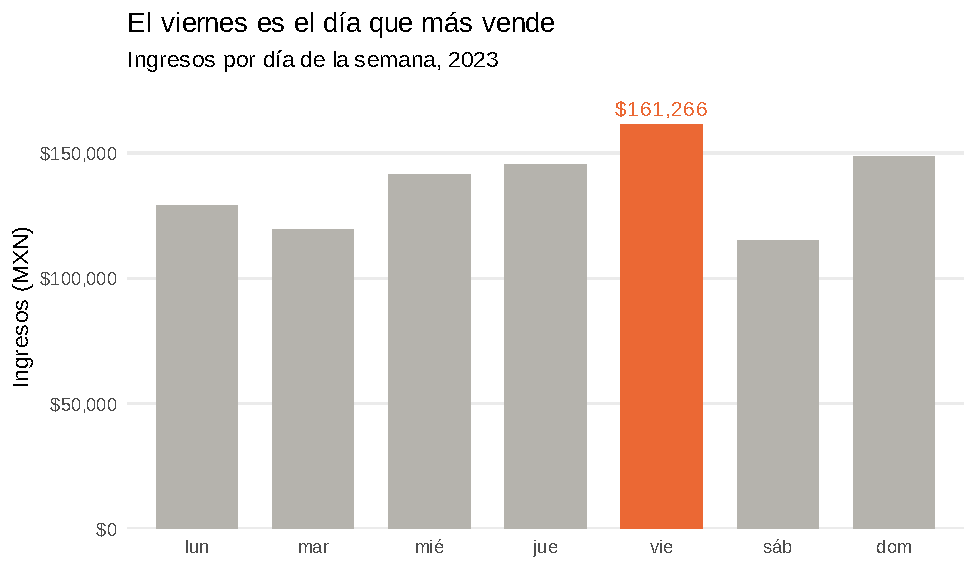
\includegraphics[width=0.85\textwidth]{m03-sol-dia}
\caption{Solución del ejercicio m3-5.}
\label{fig:m03-sol-dia}
\end{figure}

\textbf{Interpretación.} El viernes suma \$161,266, contra \$115,172 del
sábado, el día más bajo. Pero recuerda el mapa de calor
(figura~\ref{fig:m03-calor}): el viernes no es el mejor día \emph{todos}
los meses. La diferencia anual existe, pero no es tan consistente como para
basar en ella una estrategia sin más análisis.


\begin{solucion}{m3-6}
Este es el código completo, con su salida y la interpretación.
\end{solucion}

\begin{rcode}
library(tidyverse)
library(scales)
empleados <- read_csv("datasets/empleados.csv", show_col_types = FALSE)

empleados %>%
  group_by(departamento) %>%
  summarise(mediana = median(salario_mensual),
            ric     = IQR(salario_mensual),   # rango intercuartílico
            n       = n(),
            .groups = "drop") %>%
  arrange(desc(mediana))

s6 <- ggplot(empleados,
             aes(x = salario_mensual,
                 y = fct_reorder(departamento, salario_mensual,
                                 .fun = median))) +
  geom_boxplot(fill = "#cde2fb", color = "#2a78d6", width = 0.6) +
  scale_x_continuous(labels = dollar) +
  labs(title = "IT y Operaciones tienen los salarios medianos más altos",
       x = "Salario mensual (MXN)", y = NULL) +
  theme_minimal() +
  theme(panel.grid.minor = element_blank(),
        panel.grid.major.y = element_blank())
s6
\end{rcode}
\begin{rsalida}
# A tibble: 7 x 4
  departamento        mediana    ric     n
  <chr>                 <dbl>  <dbl> <int>
1 IT                   35044. 20725.     9
2 Operaciones          34945. 17114.    10
3 Ventas               32102. 22089.    16
4 Finanzas             31123. 14796.     9
5 Atención al Cliente  30663. 17242.    29
6 Marketing            24193. 11419.    12
7 RRHH                 18291. 13712.    15
\end{rsalida}

\textbf{Interpretación.} IT y Operaciones tienen las medianas más altas
(unos \$35,000) y RRHH la más baja (\$18,291). La mayor dispersión la
tiene Ventas: su rango intercuartílico (\codigo{ric}, el ancho de la caja)
es de \$22,089. Cuidado: algunos departamentos tienen
solo 9 o 10 personas, así que un boxplot con tan pocos datos es
orientativo; siempre acompáñalo del número de observaciones.


\begin{solucion}{m3-7}
Este es el código completo, con su salida y la interpretación.
\end{solucion}

\begin{rcode}
library(tidyverse)
library(scales)
color_principal <- "#2a78d6"
color_resalte   <- "#eb6834"
color_gris      <- "#b5b3ad"

productos <- read_csv("datasets/productos.csv", show_col_types = FALSE)

productos_margen <- productos %>%
  mutate(situacion = if_else(costo > precio_catalogo,
                             "Costo mayor al precio",
                             "Margen positivo"))
count(productos_margen, situacion)

s_costo <- ggplot(productos_margen,
                  aes(x = costo, y = precio_catalogo,
                      color = situacion)) +
  geom_abline(slope = 1, intercept = 0, linetype = "dashed",
              color = color_gris) +
  geom_point(size = 2.5, alpha = 0.8) +
  annotate("text", x = 380, y = 390, label = "precio = costo",
           angle = 20, size = 3, color = "#52514e", vjust = -0.5) +
  scale_color_manual(values = c("Margen positivo" = color_principal,
                                "Costo mayor al precio" = color_resalte)) +
  scale_x_continuous(labels = dollar) +
  scale_y_continuous(labels = dollar) +
  labs(title = "10 de 50 productos cuestan más de lo que se venden",
       subtitle = "Cada punto es un producto del catálogo",
       x = "Costo", y = "Precio de catálogo", color = NULL) +
  theme_minimal() +
  theme(panel.grid.minor = element_blank(),
        legend.position = "top")
s_costo
\end{rcode}
\begin{rsalida}
# A tibble: 2 x 2
  situacion                 n
  <chr>                 <int>
1 Costo mayor al precio    10
2 Margen positivo          40
\end{rsalida}

\begin{figure}[H]
\centering
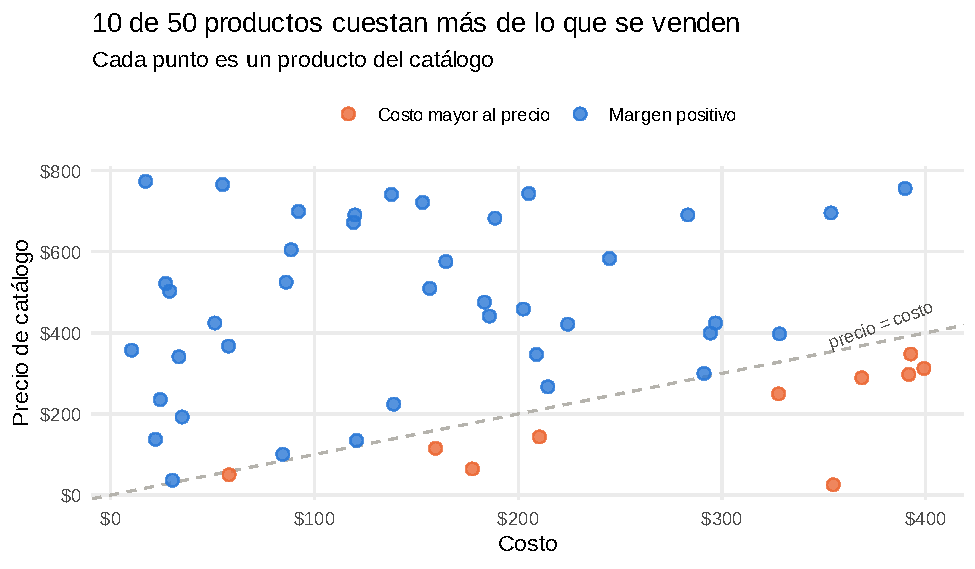
\includegraphics[width=0.85\textwidth]{m03-sol-costo}
\caption{Solución del ejercicio m3-7: los puntos naranjas, debajo de la
diagonal, tienen margen negativo.}
\label{fig:m03-sol-costo}
\end{figure}

\textbf{Interpretación.} Todo punto por debajo de la diagonal tiene un
costo mayor a su precio: 10 de los 50 productos (20\%). Es un
\emph{hallazgo de calidad de datos} o de negocio que hay que escalar: o el
costo está mal capturado, o se están vendiendo productos con pérdida. Al
área de compras le pedirías revisar primero estos diez productos.


\begin{solucion}{m3-8}
La clave es dibujar dos capas con datos distintos: primero las siete
tiendas en gris (con \codigo{group} para que cada una sea su propia línea y
sin \codigo{color} en \codigo{aes()}, así no entran a la leyenda) y encima
las tres líderes con \codigo{color = tienda}.
\end{solucion}

\begin{rcode}
library(tidyverse)
library(scales)
color_gris   <- "#b5b3ad"
paleta_libro <- c("#2a78d6", "#eb6834", "#1baf7a", "#eda100",
                  "#e87ba4", "#008300", "#4a3aa7", "#e34948")

transacciones <- read_csv("datasets/transacciones.csv",
                          show_col_types = FALSE)
tiendas <- read_csv("datasets/tiendas.csv", show_col_types = FALSE)

acumulado <- transacciones %>%
  left_join(tiendas, by = "tienda_id") %>%
  mutate(tienda = str_remove(nombre_tienda, "Sucursal "),
         mes = floor_date(fecha, unit = "month")) %>%
  group_by(tienda, mes) %>%
  summarise(ingresos = sum(total_transaccion), .groups = "drop") %>%
  group_by(tienda) %>%
  arrange(mes, .by_group = TRUE) %>%
  mutate(acumulado = cumsum(ingresos)) %>%
  ungroup()

# las 3 con más ingresos acumulados en el último mes
top3 <- acumulado %>%
  filter(mes == max(mes)) %>%
  slice_max(acumulado, n = 3) %>%
  pull(tienda)
top3

lideres <- acumulado %>%
  filter(tienda %in% top3) %>%
  mutate(tienda = factor(tienda, levels = top3))  # orden de la leyenda
resto <- acumulado %>% filter(!tienda %in% top3)

s_top3 <- ggplot(mapping = aes(x = mes, y = acumulado)) +
  geom_line(data = resto, aes(group = tienda),
            color = color_gris, linewidth = 0.5) +
  geom_line(data = lideres, aes(color = tienda), linewidth = 0.9) +
  scale_color_manual(values = paleta_libro[1:3]) +
  scale_x_date(date_labels = "%b", date_breaks = "1 month") +
  scale_y_continuous(labels = dollar) +
  labs(title = "Las tres tiendas líderes al cierre de 2023",
       subtitle = "Ingresos acumulados; en gris, las otras 7 tiendas",
       x = NULL, y = "Ingresos acumulados (MXN)", color = NULL) +
  theme_minimal() +
  theme(panel.grid.minor = element_blank(),
        legend.position = "top")
s_top3
\end{rcode}
\begin{rsalida}
[1] "Outlet"  "Sur"     "Plaza A"
\end{rsalida}

\begin{figure}[H]
\centering
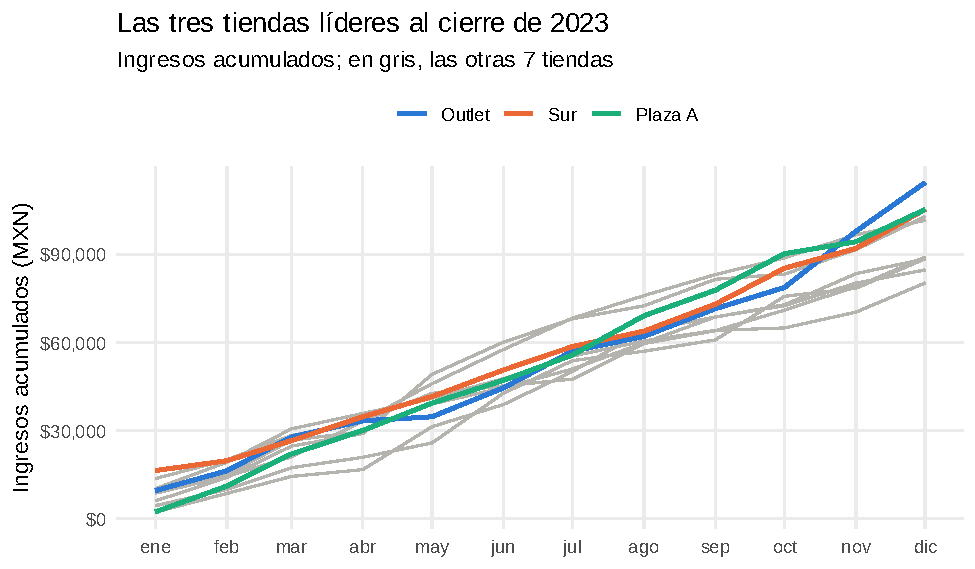
\includegraphics[width=0.85\textwidth]{m03-sol-top3}
\caption{Solución del ejercicio m3-8.}
\label{fig:m03-sol-top3}
\end{figure}

\textbf{Interpretación.} Outlet, Sur y Plaza A terminan arriba. Sur y
Plaza A cierran prácticamente empatadas (\$105,305 y \$105,216). El
primer lugar cambió de manos varias veces durante el año y Outlet lo tomó
en noviembre. Como \codigo{top3} se calcula con código, la gráfica se
actualiza sola si cambian los datos.


\begin{solucion}{m3-9}
Dentro de una función, \codigo{\{\{ categoria \}\}} (se lee
``\emph{curly-curly}'') le dice a \paquete{ggplot2} y a \paquete{dplyr} que
use la columna cuyo nombre recibió el argumento.
\end{solucion}

\begin{rcode}
library(tidyverse)
library(scales)
color_principal <- "#2a78d6"

tema_empresa <- function(base_size = 11) {
  theme_minimal(base_size = base_size) +
    theme(plot.title = element_text(face = "bold", color = "#0b0b0b"),
          plot.title.position = "plot",
          axis.text = element_text(color = "#52514e"),
          panel.grid.minor = element_blank(),
          panel.grid.major.y = element_blank(),
          plot.margin = margin(10, 15, 10, 10))
}

grafica_ranking <- function(datos, categoria, valor, titulo) {
  ggplot(datos, aes(x = {{ valor }},
                    y = fct_reorder({{ categoria }}, {{ valor }}))) +
    geom_col(fill = color_principal, width = 0.7) +
    scale_x_continuous(labels = dollar,
                       expand = expansion(mult = c(0, 0.05))) +
    labs(title = titulo, x = NULL, y = NULL) +
    tema_empresa()
}

transacciones <- read_csv("datasets/transacciones.csv",
                          show_col_types = FALSE)
tiendas <- read_csv("datasets/tiendas.csv", show_col_types = FALSE)

por_pago <- transacciones %>%
  group_by(metodo_pago) %>%
  summarise(ingresos = sum(total_transaccion), .groups = "drop")

por_tienda <- transacciones %>%
  left_join(tiendas, by = "tienda_id") %>%
  group_by(nombre_tienda) %>%
  summarise(ingresos = sum(total_transaccion), .groups = "drop")

g_pago <- grafica_ranking(por_pago, metodo_pago, ingresos,
                          "Tarjeta de crédito, el método más usado")
g_tienda <- grafica_ranking(por_tienda, nombre_tienda, ingresos,
                            "Sucursal Outlet lidera en ingresos")

dir.create("resultados", showWarnings = FALSE)
ggsave("resultados/ranking_pago.png", g_pago, width = 7, height = 4,
       dpi = 300, bg = "white")
ggsave("resultados/ranking_tienda.png", g_tienda, width = 7, height = 4,
       dpi = 300, bg = "white")
file.exists(c("resultados/ranking_pago.png",
              "resultados/ranking_tienda.png"))
\end{rcode}
\begin{rsalida}
[1] TRUE TRUE
\end{rsalida}

\textbf{Interpretación.} Con una sola función produces gráficas idénticas
en estilo para cualquier tabla con una columna de categoría y otra de
valor. Es el primer paso hacia un ``kit'' de gráficas del área de BI.


\begin{solucion}{m3-10}
Este es el código completo, con su salida y la interpretación.
\end{solucion}

\begin{rcode}
library(tidyverse)
library(scales)
color_principal <- "#2a78d6"
color_resalte   <- "#eb6834"
color_gris      <- "#b5b3ad"

clientes <- read_csv("datasets/clientes.csv", show_col_types = FALSE)

# (a) KPIs en consola
cat("Clientes totales:", comma(nrow(clientes)), "\n")
cat("% premium:", percent(mean(clientes$es_premium), accuracy = 0.1),
    "\n")
cat("Edad mediana:", median(clientes$edad), "años\n")

# (b) clientes por ciudad, resaltando la mayor
clientes_ciudad <- clientes %>%
  count(ciudad, name = "clientes") %>%
  mutate(destacar = if_else(clientes == max(clientes), "Mayor",
                            "Resto"))

s_ciudades <- ggplot(clientes_ciudad,
                     aes(x = clientes,
                         y = fct_reorder(ciudad, clientes),
                         fill = destacar)) +
  geom_col(width = 0.7) +
  geom_text(aes(label = clientes), hjust = -0.3, size = 3.2,
            color = "#52514e") +
  scale_fill_manual(values = c(Mayor = color_resalte,
                               Resto = color_gris),
                    guide = "none") +
  scale_x_continuous(expand = expansion(mult = c(0, 0.1))) +
  labs(title = "Puebla encabeza por poco: 28 clientes contra 27 de CDMX",
       subtitle = "Clientes registrados por ciudad",
       x = "Clientes", y = NULL,
       caption = "Fuente: clientes.csv") +
  theme_minimal() +
  theme(panel.grid.minor = element_blank(),
        panel.grid.major.y = element_blank())
s_ciudades
\end{rcode}
\begin{rsalida}
Clientes totales: 200 
% premium: 36.5% 
Edad mediana: 48.5 años
\end{rsalida}

\begin{figure}[H]
\centering
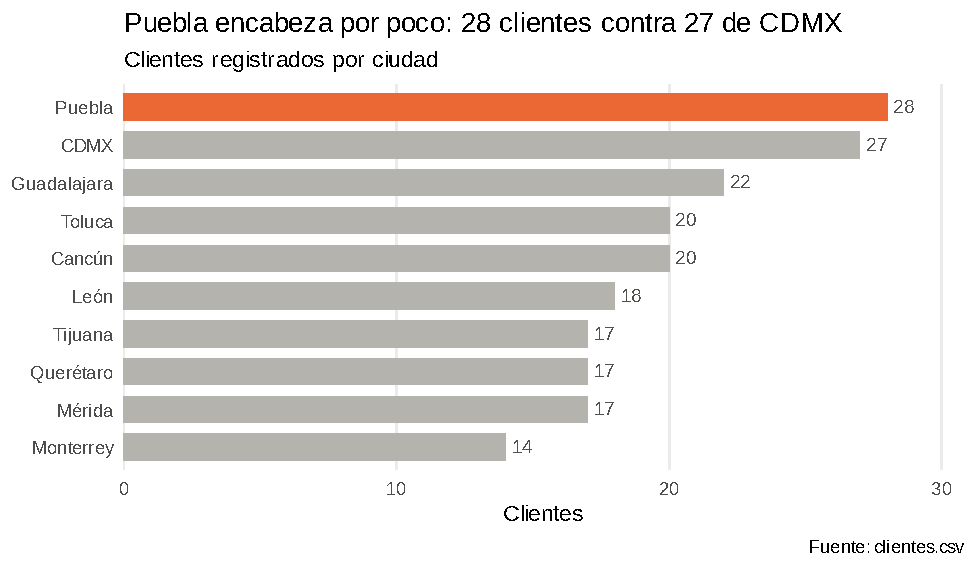
\includegraphics[width=0.85\textwidth]{m03-sol-ciudades}
\caption{Solución del ejercicio m3-10, inciso (b).}
\label{fig:m03-sol-ciudades}
\end{figure}

Para el inciso (c), el porcentaje de premium por segmento es el promedio
de la columna lógica \codigo{es\_premium} (\codigo{TRUE} cuenta como 1).
Ordenamos los segmentos por edad, no por valor, porque tienen un orden
natural.

\begin{rcode}
premium_segmento <- clientes %>%
  mutate(segmento = factor(segmento,
                           levels = c("Joven", "Adulto", "Maduro",
                                      "Senior"))) %>%
  group_by(segmento) %>%
  summarise(clientes = n(), pct_premium = mean(es_premium),
            .groups = "drop")
premium_segmento

s_premium <- ggplot(premium_segmento,
                    aes(x = segmento, y = pct_premium)) +
  geom_col(fill = color_principal, width = 0.6) +
  geom_text(aes(label = percent(pct_premium, accuracy = 1)),
            vjust = -0.5, size = 3.5, color = "#52514e") +
  scale_y_continuous(labels = percent, limits = c(0, 0.5),
                     expand = expansion(mult = c(0, 0.05))) +
  labs(title = "El segmento Maduro tiene más clientes premium",
       subtitle = "% de clientes premium por segmento de edad",
       x = NULL, y = NULL, caption = "Fuente: clientes.csv") +
  theme_minimal() +
  theme(panel.grid.minor = element_blank(),
        panel.grid.major.x = element_blank())

dir.create("resultados", showWarnings = FALSE)
ggsave("resultados/clientes_ciudad.png", s_ciudades, width = 7,
       height = 4, dpi = 300, bg = "white")
ggsave("resultados/premium_segmento.png", s_premium, width = 7,
       height = 4, dpi = 300, bg = "white")
\end{rcode}
\begin{rsalida}
# A tibble: 4 x 3
  segmento clientes pct_premium
  <fct>       <int>       <dbl>
1 Joven          21       0.333
2 Adulto         48       0.312
3 Maduro         70       0.414
4 Senior         61       0.361
\end{rsalida}

\textbf{Conclusiones para marketing.}
\begin{enumerate}
  \item Tenemos 200 clientes, 36.5\% premium, con edad mediana de 48.5
        años: la base es madura.
  \item Puebla (28) y CDMX (27) concentran el 27.5\% de los clientes;
        Monterrey es la ciudad con menos (14), una posible oportunidad de
        crecimiento.
  \item El segmento Maduro (41--60 años) es el más grande (70 clientes) y el
        de mayor proporción premium (41\%); los Jóvenes son pocos (21), así
        que su 33\% premium se basa en muy pocos casos.
\end{enumerate}



\section{Módulo 4. Análisis exploratorio y estadística}
% ============================================================================
% SOLUCIONES DEL MÓDULO 4
% ============================================================================

\begin{solucion}{m4-1}
Cargamos los datos y calculamos cada medida sobre \codigo{precio\_venta}.

\begin{rcode}
library(tidyverse)
options(cli.unicode = FALSE)
transacciones <- read_csv("datasets/transacciones.csv",
                          show_col_types = FALSE)
\end{rcode}

\begin{rcode}
precio <- transacciones$precio_venta

c(media    = mean(precio),
  mediana  = median(precio),
  desv_est = sd(precio),
  cv       = sd(precio) / mean(precio),
  iqr      = IQR(precio))
quantile(precio, probs = c(0.10, 0.90))
\end{rcode}
\begin{rsalida}
      media     mediana    desv_est          cv         iqr
318.3110300 324.9200000 171.5302293   0.5388762 303.8950000
    10%     90%
 76.705 545.047
\end{rsalida}

La media (\$318.31) y la mediana (\$324.92) son casi iguales: la
distribución del precio es simétrica (recuerda que su asimetría era
$-0.08$). El coeficiente de variación es 0.54, menor que el del ticket
(0.79): el precio varía menos en términos relativos porque el ticket
multiplica dos fuentes de variación (precio y cantidad). El 80\% central de
los precios está entre \$73 y \$541.
\end{solucion}

\begin{solucion}{m4-2}
Definimos la función \codigo{moda()} y luego armamos la tabla por día.

\begin{rcode}
library(tidyverse)
transacciones <- read_csv("datasets/transacciones.csv",
                          show_col_types = FALSE)

moda <- function(x) {
  frecuencias <- table(x)
  names(frecuencias)[which.max(frecuencias)]
}
\end{rcode}

\begin{rcode}
moda(transacciones$dia_semana)

transacciones %>%
  group_by(dia_semana) %>%
  summarise(transacciones = n(),
            ventas = sum(total_transaccion),
            .groups = "drop") %>%
  mutate(pct_transacciones = transacciones / sum(transacciones)) %>%
  arrange(desc(transacciones))
\end{rcode}
\begin{rsalida}
[1] "viernes"
# A tibble: 7 x 4
  dia_semana transacciones  ventas pct_transacciones
  <chr>              <int>   <dbl>             <dbl>
1 viernes              158 161266.             0.158
2 miércoles            155 141329.             0.155
3 domingo              146 148703.             0.146
4 jueves               146 145280.             0.146
5 lunes                136 128878.             0.136
6 sábado               130 115172.             0.13
7 martes               129 119364.             0.129
\end{rsalida}

El viernes es el día con más transacciones (moda). Revisa la columna
\codigo{ventas}: el orden por ventas no coincide exactamente con el orden
por número de transacciones, porque el ticket promedio cambia de un día a
otro. Para programar personal importa el número de transacciones; para
metas de venta, el monto.
\end{solucion}

\begin{solucion}{m4-3}
\begin{rcode}
library(tidyverse)
empleados <- read_csv("datasets/empleados.csv", show_col_types = FALSE)
\end{rcode}

\begin{rcode}
empleados %>%
  group_by(departamento) %>%
  summarise(empleados  = n(),
            media      = mean(salario_mensual),
            mediana    = median(salario_mensual),
            diferencia = media - mediana,
            .groups = "drop") %>%
  arrange(desc(abs(diferencia)))
\end{rcode}
\begin{rsalida}
# A tibble: 7 x 5
  departamento        empleados  media mediana diferencia
  <chr>                   <int>  <dbl>   <dbl>      <dbl>
1 RRHH                       15 22956.  18291.      4665.
2 Operaciones                10 30380.  34945.     -4566.
3 IT                          9 30842.  35044.     -4202.
4 Ventas                     16 29032.  32102.     -3071.
5 Finanzas                    9 28116.  31123.     -3007.
6 Atención al Cliente        29 27919.  30663.     -2745.
7 Marketing                  12 24602.  24193.       410.
\end{rsalida}

En RRHH la media supera a la mediana por unos \$4,665: hay algunos
salarios altos que la jalan hacia arriba, mientras que la mitad de los 15
empleados gana menos de \$18,291. Para anunciar el ``salario típico'' de RRHH
conviene la mediana. En IT y Operaciones pasa lo contrario (media menor que
la mediana): hay salarios bajos que la jalan hacia abajo. Nota que algunos
departamentos tienen muy pocos empleados (9 en Finanzas e IT), así que sus
medidas son poco estables.
\end{solucion}

\begin{solucion}{m4-4}
\begin{rcode}
library(tidyverse)
ventas <- read_csv("datasets/ventas_retail.csv", show_col_types = FALSE)
\end{rcode}

\begin{rcode}
q1 <- quantile(ventas$total, 0.25)
q3 <- quantile(ventas$total, 0.75)
limite_superior <- unname(q3 + 1.5 * (q3 - q1))
limite_superior

ventas_marcadas <- ventas %>%
  mutate(atipico_iqr = total < q1 - 1.5 * (q3 - q1) |
                       total > limite_superior,
         z = (total - mean(total)) / sd(total),
         atipico_z = abs(z) > 3)

sum(ventas_marcadas$atipico_iqr)   # regla IQR
sum(ventas_marcadas$atipico_z)     # regla z

ventas_marcadas %>%
  filter(atipico_iqr) %>%
  select(fecha, cantidad, precio_unitario, descuento_pct, total, z)

# Asimetría
mean((ventas$total - mean(ventas$total))^3) / sd(ventas$total)^3
\end{rcode}
\begin{rsalida}
[1] 4751.18
[1] 3
[1] 3
# A tibble: 3 x 6
  fecha      cantidad precio_unitario descuento_pct total     z
  <date>        <dbl>           <dbl>         <dbl> <dbl> <dbl>
1 2023-04-21       10            492.             0 4925.  3.13
2 2023-07-24       10            495.             0 4950.  3.15
3 2023-09-04       10            487.             0 4875.  3.08
[1] 0.8517708
\end{rsalida}

La regla del IQR marca 3 ventas (todas por encima de \$4,751) y la regla $z$
ninguna. Las tres son ventas de 10 unidades a precios altos (más de \$480)
con poco o ningún descuento: son ventas grandes \emph{legítimas}, no
errores, así que se conservan. La asimetría de 0.85 confirma una cola
moderada a la derecha, como la del ticket de \archivo{transacciones.csv}.
\end{solucion}

\begin{solucion}{m4-5}
\begin{rcode}
library(tidyverse)
library(scales)
ventas <- read_csv("datasets/ventas_retail.csv", show_col_types = FALSE)
\end{rcode}

\begin{rcode}
meta_trimestral <- 130000

kpi_trimestral <- ventas %>%
  group_by(trimestre) %>%
  summarise(ventas = sum(total), .groups = "drop") %>%
  arrange(trimestre) %>%
  mutate(crec_qoq   = ventas / lag(ventas) - 1,
         acumulado  = cumsum(ventas),
         indice_100 = ventas / first(ventas) * 100,
         vs_meta    = ventas / meta_trimestral - 1)
kpi_trimestral

sum(kpi_trimestral$vs_meta >= 0)            # trimestres en meta
sum(kpi_trimestral$ventas) / (4 * meta_trimestral) - 1   # vs meta anual
\end{rcode}
\begin{rsalida}
# A tibble: 4 x 6
  trimestre  ventas crec_qoq acumulado indice_100 vs_meta
  <chr>       <dbl>    <dbl>     <dbl>      <dbl>   <dbl>
1 Q1        126274.  NA        126274.      100   -0.0287
2 Q2        120717.  -0.0440   246991.       95.6 -0.0714
3 Q3        134427.   0.114    381418.      106.   0.0341
4 Q4        132498.  -0.0144   513917.      105.   0.0192
[1] 2
[1] -0.01169883
\end{rsalida}

Solo el tercer y el cuarto trimestre superaron la meta de \$130,000 (Q3 por
3.4\% y Q4 por 1.9\%). El segundo trimestre cayó 4.4\% contra el primero y
el tercero creció 11.4\%. En el año, las ventas quedaron 0.8\% por debajo de
la meta anual de \$520,000: la recuperación del segundo semestre no alcanzó
para compensar el primero.
\end{solucion}

\begin{solucion}{m4-6}
$H_0$: el número promedio de compras por cliente es igual en premium y no
premium. $H_1$: es distinto. Usamos $\alpha = 0.05$.

\begin{rcode}
library(tidyverse)
transacciones <- read_csv("datasets/transacciones.csv",
                          show_col_types = FALSE)
clientes <- read_csv("datasets/clientes.csv", show_col_types = FALSE)
\end{rcode}

\begin{rcode}
frecuencia <- transacciones %>%
  count(cliente_id, name = "compras") %>%          # compras por cliente
  left_join(clientes, by = "cliente_id")

frecuencia %>%
  group_by(es_premium) %>%
  summarise(clientes = n(), compras_prom = mean(compras),
            .groups = "drop")

t.test(compras ~ es_premium, data = frecuencia)
\end{rcode}
\begin{rsalida}
# A tibble: 2 x 3
  es_premium clientes compras_prom
  <lgl>         <int>        <dbl>
1 FALSE           126         5.18
2 TRUE             72         4.82

        Welch Two Sample t-test

data:  compras by es_premium
t = 1.063, df = 146.53, p-value = 0.2895
alternative hypothesis: true difference in means between group FALSE and group TRUE is not equal to 0
95 percent confidence interval:
 -0.3119807  1.0381711
sample estimates:
mean in group FALSE  mean in group TRUE
           5.182540            4.819444
\end{rsalida}

Los clientes premium compraron en promedio 5.2 veces en el año y los no
premium 5.0: una diferencia de apenas 0.2 compras. Con $p = 0.61$ no
rechazamos $H_0$. Conclusión para la directora: \emph{con los datos de 2023
no hay evidencia de que los clientes premium compren con más frecuencia ni
gasten más por ticket que los demás; el programa premium no está cambiando
el comportamiento de compra}. Solo se incluyen los 198 clientes con al menos
una compra.
\end{solucion}

\begin{solucion}{m4-7}
\begin{rcode}
library(tidyverse)
transacciones <- read_csv("datasets/transacciones.csv",
                          show_col_types = FALSE)
\end{rcode}

\begin{rcode}
abc_clientes <- transacciones %>%
  group_by(cliente_id) %>%
  summarise(gasto = sum(total_transaccion), .groups = "drop") %>%
  arrange(desc(gasto)) %>%
  mutate(pct_acumulado = cumsum(gasto) / sum(gasto),
         pct_clientes  = row_number() / n(),
         clase = case_when(pct_acumulado <= 0.80 ~ "A",
                           pct_acumulado <= 0.95 ~ "B",
                           TRUE                  ~ "C"))

abc_clientes %>%
  group_by(clase) %>%
  summarise(clientes = n(),
            pct_clientes = n() / nrow(abc_clientes),
            pct_ingresos = sum(gasto) / sum(abc_clientes$gasto),
            .groups = "drop")

# Participación del 20% de clientes que más gasta
abc_clientes %>%
  filter(pct_clientes <= 0.20) %>%
  summarise(clientes = n(), pct_ingresos = max(pct_acumulado))
\end{rcode}
\begin{rsalida}
# A tibble: 3 x 4
  clase clientes pct_clientes pct_ingresos
  <chr>    <int>        <dbl>        <dbl>
1 A          119        0.601       0.798
2 B           44        0.222       0.151
3 C           35        0.177       0.0511
# A tibble: 1 x 2
  clientes pct_ingresos
     <int>        <dbl>
1       39        0.367
\end{rsalida}

Se necesitan 116 clientes (el 58.6\% de la clientela activa) para juntar el
80\% de los ingresos, y el 20\% de clientes que más gasta aporta el 37.2\%.
Los ingresos están más concentrados en clientes que en productos (donde el
20\% superior aportaba el 26.4\%), pero siguen lejos de la regla 80/20.
Para la empresa significa que un programa de lealtad no puede enfocarse en
unos cuantos clientes: la base de clientes valiosos es amplia.
\end{solucion}

\begin{solucion}{m4-8}
\begin{rcode}
# 1. Normal: ventas semanales
pnorm(20000, mean = 18445, sd = 4591) -
  pnorm(15000, mean = 18445, sd = 4591)       # P(15,000 < X < 20,000)
qnorm(0.95, mean = 18445, sd = 4591)          # se supera 5% de las veces

# 2. Binomial: devoluciones de 150 ventas con p = 0.03
1 - pbinom(8, size = 150, prob = 0.03)        # P(más de 8)
dbinom(0, size = 150, prob = 0.03)            # P(ninguna)

# 3. Poisson: llamadas en 10 minutos con lambda = 4
1 - ppois(7, lambda = 4)                      # P(8 o más)
\end{rcode}
\begin{rsalida}
[1] 0.4060719
[1] 25996.52
[1] 0.03780957
[1] 0.01036956
[1] 0.05113362
\end{rsalida}

\begin{enumerate}
  \item Hay un 40.6\% de probabilidad de que una semana venda entre
        \$15,000 y \$20,000. Solo el 5\% de las semanas supera \$25,997.
  \item Con 150 ventas se esperan $150 \times 0.03 = 4.5$ devoluciones. Tener
        más de 8 ocurre el 3.9\% de los días; no tener ninguna, solo el
        1.0\%.
  \item Recibir 8 o más llamadas en 10 minutos tiene una probabilidad de
        5.1\%: pasa en uno de cada 20 intervalos, útil para dimensionar el
        personal del centro de atención.
\end{enumerate}
Observa los detalles de ``más de'' y ``o más'': $P(X > 8) = 1 - P(X \leq 8)$,
pero $P(X \geq 8) = 1 - P(X \leq 7)$.
\end{solucion}

\begin{solucion}{m4-9}
\textbf{1. Prueba A/B.} $H_0$: las dos tasas de conversión son iguales.

\begin{rcode}
compras <- c(A = 180, B = 225)
visitas <- c(A = 3000, B = 3000)
compras / visitas                    # tasas de conversión
prop.test(x = compras, n = visitas)
\end{rcode}
\begin{rsalida}
    A     B
0.060 0.075

        2-sample test for equality of proportions with continuity
        correction

data:  compras out of visitas
X-squared = 5.1263, df = 1, p-value = 0.02357
alternative hypothesis: two.sided
95 percent confidence interval:
 -0.028024006 -0.001975994
sample estimates:
prop 1 prop 2
 0.060  0.075
\end{rsalida}

El diseño A convierte 6.0\% y el B 7.5\%. Con $p = 0.024 < 0.05$ rechazamos
$H_0$: el diseño B convierte más. La diferencia real está entre 0.2 y 2.8
puntos porcentuales a favor de B (R la reporta como A menos B, por eso los
signos negativos).

\textbf{2. ANOVA de salarios por departamento.}

\begin{rcode}
library(tidyverse)
empleados <- read_csv("datasets/empleados.csv", show_col_types = FALSE)
\end{rcode}

\begin{rcode}
modelo_salarios <- aov(salario_mensual ~ departamento, data = empleados)
summary(modelo_salarios)
\end{rcode}
\begin{rsalida}
             Df    Sum Sq   Mean Sq F value Pr(>F)
departamento  6 6.399e+08 106656199   0.876  0.516
Residuals    93 1.133e+10 121778750
\end{rsalida}

El p-valor es 0.516: no hay evidencia de que el salario promedio difiera
entre departamentos. Como el ANOVA no es significativo, \textbf{no tiene
sentido} aplicar \codigo{TukeyHSD()} buscando qué par es distinto: sería
buscar diferencias donde la prueba global dice que no las hay (una forma de
p-hacking). Además, los datos de salarios son simulados al azar, así que el
resultado es el esperado.
\end{solucion}

\begin{solucion}{m4-10}
\begin{rcode}
library(tidyverse)
set.seed(123)
semanas <- tibble(
  precio = runif(52, min = 80, max = 120)
) %>%
  mutate(unidades = 500 - 3 * precio + rnorm(52, sd = 15))
\end{rcode}

\textbf{1. Regresión.}

\begin{rcode}
modelo_precio <- lm(unidades ~ precio, data = semanas)
coef(modelo_precio)
confint(modelo_precio)
summary(modelo_precio)$r.squared
\end{rcode}
\begin{rsalida}
(Intercept)      precio
 498.510218   -2.973617
                2.5 %     97.5 %
(Intercept) 465.24655 531.773889
precio       -3.30276  -2.644474
[1] 0.8681726
\end{rsalida}

La pendiente estimada es $-3.13$: por cada peso que sube el precio, se
venden en promedio 3.1 unidades menos a la semana. Su intervalo del 95\%
(de $-3.63$ a $-2.64$) contiene el valor real de $-3$, así que la regresión
recuperó la relación simulada. El $R^2$ de 0.76 indica que el precio explica
el 76\% de la variación de las unidades.

\textbf{2 y 3. Predicciones.}

\begin{rcode}
predict(modelo_precio, newdata = tibble(precio = 100),
        interval = "prediction")
predict(modelo_precio, newdata = tibble(precio = 200))
range(semanas$precio)       # rango de precios observado
\end{rcode}
\begin{rsalida}
       fit      lwr      upr
1 201.1485 173.0502 229.2469
        1
-96.21315
[1]  80.98455 119.77079
\end{rsalida}

Con un precio de \$100 esperamos vender unas 196 unidades en la semana,
con un intervalo de predicción de 164 a 228. Con \$200 el modelo predice
unidades \emph{negativas}, algo imposible: los precios observados van de
\$80 a \$120 y fuera de ese rango no sabemos si la relación sigue siendo
lineal. Es un ejemplo claro de por qué no se debe extrapolar.

\textbf{4. Residuos.}

\begin{rcode}
diagnostico <- tibble(ajustado = fitted(modelo_precio),
                      residuo  = residuals(modelo_precio))
summary(diagnostico$residuo)
# Correlación entre residuos y ajustados (debe ser ~0)
round(cor(diagnostico$ajustado, diagnostico$residuo), 4)

ggplot(diagnostico, aes(x = ajustado, y = residuo)) +
  geom_hline(yintercept = 0, color = "#eb6834") +
  geom_point(color = "#2a78d6") +
  labs(x = "Unidades ajustadas", y = "Residuo") +
  theme_minimal()
\end{rcode}
\begin{rsalida}
   Min. 1st Qu.  Median    Mean 3rd Qu.    Max.
-35.405  -8.198  -1.030   0.000  10.582  31.869
[1] 0
\end{rsalida}

Los residuos están centrados en cero (mediana cercana a 0), son más o menos
simétricos y no guardan relación con los valores ajustados. En la gráfica
deberías ver una nube sin patrón: el modelo lineal es adecuado dentro del
rango de precios observado.
\end{solucion}


\section{Módulo 5. Bases de datos, SQL y ETL}
% ============================================================================
% Soluciones del Módulo 5 - Bases de datos, SQL y ETL desde R
% ============================================================================

\begin{solucion}{m5-1}
Creamos la base en memoria, cargamos el CSV con \codigo{dbWriteTable()} y
exploramos. Primero los paquetes (en todas las soluciones de este módulo
usamos los mismos):

\begin{rcode}
library(tidyverse)
library(DBI)
library(RSQLite)
library(dbplyr)
\end{rcode}

\begin{rcode}
con <- dbConnect(RSQLite::SQLite(), ":memory:")

productos <- read_csv("datasets/productos.csv", show_col_types = FALSE)
dbWriteTable(con, "productos", productos)

dbListTables(con)
dbListFields(con, "productos")

dbGetQuery(con, "
  SELECT categoria,
         COUNT(*)                      AS productos,
         ROUND(AVG(precio_catalogo), 2) AS precio_promedio
  FROM productos
  GROUP BY categoria
  ORDER BY productos DESC, categoria
")

dbDisconnect(con)
\end{rcode}

\begin{rsalida}
[1] "productos"
 [1] "producto_id"     "nombre_producto" "categoria"      
 [4] "subcategoria"    "marca"           "precio_catalogo"
 [7] "costo"           "stock_actual"    "stock_minimo"   
[10] "proveedor"       "activo"          "margen_pct"     
[13] "estado_stock"   
     categoria productos precio_promedio
1      Belleza         9          474.54
2  Electrónica         7          413.72
3    Alimentos         6          354.92
4     Juguetes         6          425.89
5   Automotriz         5          365.35
6     Deportes         4          452.79
7       Libros         4          500.17
8     Mascotas         4          388.89
9        Hogar         3          361.51
10        Ropa         2          357.82
\end{rsalida}

La tabla tiene 13 columnas. Belleza es la categoría con más productos (9) y
Ropa la que menos (2). Libros tiene el precio de catálogo promedio más
alto (\$500.17), aunque con solo 4 productos.
\end{solucion}

\begin{solucion}{m5-2}
El filtro combina dos condiciones con \codigo{AND}; el faltante es una
columna calculada con alias, que podemos usar en el \codigo{ORDER BY}.

\begin{rcode}
con <- dbConnect(RSQLite::SQLite(), ":memory:")
dbWriteTable(con, "productos",
             read_csv("datasets/productos.csv", show_col_types = FALSE))

alerta <- dbGetQuery(con, "
  SELECT nombre_producto, categoria, proveedor, stock_actual,
         stock_minimo, stock_minimo - stock_actual AS faltante
  FROM productos
  WHERE activo = 1                       -- TRUE se guardó como 1
    AND stock_actual < stock_minimo
  ORDER BY faltante DESC
")
alerta

# ¿Qué proveedor aparece más?
dbGetQuery(con, "
  SELECT proveedor, COUNT(*) AS productos_en_alerta
  FROM productos
  WHERE activo = 1 AND stock_actual < stock_minimo
  GROUP BY proveedor
  ORDER BY productos_en_alerta DESC
")
dbDisconnect(con)
\end{rcode}

\begin{rsalida}
  nombre_producto  categoria   proveedor stock_actual stock_minimo
1     Producto 03 Automotriz Proveedor 3           22           26
2     Producto 33  Alimentos Proveedor 1           42           45
3     Producto 06   Juguetes Proveedor 1           36           38
  faltante
1        4
2        3
3        2
    proveedor productos_en_alerta
1 Proveedor 1                   2
2 Proveedor 3                   1
\end{rsalida}

Solo tres productos activos están por debajo de su mínimo, todos por pocas
piezas (el Producto 03 es el más urgente, con 4 faltantes). El Proveedor 1
surte dos de ellos: es con quien conviene hablar primero.
\end{solucion}

\begin{solucion}{m5-3}
\codigo{HAVING} filtra los grupos después de agregarlos.

\begin{rcode}
con <- dbConnect(RSQLite::SQLite(), ":memory:")
dbWriteTable(con, "empleados",
             read_csv("datasets/empleados.csv", show_col_types = FALSE) %>%
               mutate(fecha_ingreso = format(fecha_ingreso, "%Y-%m-%d")))

dbGetQuery(con, "
  SELECT departamento,
         COUNT(*)                       AS empleados,
         ROUND(AVG(salario_mensual), 2) AS salario_promedio,
         MAX(salario_mensual)           AS salario_maximo
  FROM empleados
  GROUP BY departamento
  HAVING COUNT(*) >= 15
  ORDER BY salario_promedio DESC
")
dbDisconnect(con)
\end{rcode}

\begin{rsalida}
         departamento empleados salario_promedio salario_maximo
1              Ventas        16         29031.76       43777.92
2 Atención al Cliente        29         27918.75       44438.77
3                RRHH        15         22955.96       42797.09
\end{rsalida}

Solo tres departamentos tienen 15 empleados o más. Ventas paga el salario
promedio más alto (\$29\,031.76) y Atención al Cliente es el departamento
más grande (29 personas).
\end{solucion}

\begin{solucion}{m5-4}
Reutilizamos la idea de \codigo{leer\_para\_bd()} del capítulo para
guardar las fechas como texto ISO. En la parte (b), la condición de
diciembre va \emph{dentro} del \codigo{ON} del \codigo{LEFT JOIN}: si la
pusiéramos en el \codigo{WHERE}, eliminaríamos precisamente los productos
sin pareja que buscamos.

\begin{rcode}
con <- dbConnect(RSQLite::SQLite(), ":memory:")
leer_para_bd <- function(archivo) {
  read_csv(file.path("datasets", archivo), show_col_types = FALSE) %>%
    mutate(across(where(is.Date), ~ format(.x, "%Y-%m-%d")),
           across(where(hms::is_hms), as.character))
}
for (tabla in c("transacciones", "tiendas", "productos")) {
  dbWriteTable(con, tabla, leer_para_bd(paste0(tabla, ".csv")))
}

# (a) Ventas por ciudad de la tienda
dbGetQuery(con, "
  SELECT ti.ciudad,
         COUNT(*)                           AS tickets,
         ROUND(SUM(t.total_transaccion), 0) AS ventas,
         ROUND(AVG(t.total_transaccion), 2) AS ticket_promedio
  FROM transacciones AS t
  INNER JOIN tiendas AS ti ON t.tienda_id = ti.tienda_id
  GROUP BY ti.ciudad
  ORDER BY ventas DESC
")

# (b) Productos sin ventas en diciembre
dbGetQuery(con, "
  SELECT p.producto_id, p.nombre_producto, p.categoria
  FROM productos AS p
  LEFT JOIN transacciones AS t
         ON p.producto_id = t.producto_id
        AND t.fecha BETWEEN '2023-12-01' AND '2023-12-31'
  WHERE t.transaccion_id IS NULL
  ORDER BY p.producto_id
")
dbDisconnect(con)
\end{rcode}

\begin{rsalida}
       ciudad tickets ventas ticket_promedio
1        CDMX     398 383588          963.79
2 Guadalajara     184 169260          919.89
3     Tijuana     106 114377         1079.03
4   Monterrey     109 105305          966.10
5   Querétaro     108 102791          951.77
6      Puebla      95  84672          891.29
   producto_id nombre_producto   categoria
1            5     Producto 05   Alimentos
2           10     Producto 10       Hogar
3           13     Producto 13        Ropa
4           18     Producto 18      Libros
5           23     Producto 23     Belleza
6           25     Producto 25    Juguetes
7           38     Producto 38   Alimentos
8           40     Producto 40 Electrónica
9           43     Producto 43  Automotriz
10          45     Producto 45 Electrónica
11          49     Producto 49     Belleza
\end{rsalida}

CDMX concentra las ventas (\$383\,588) porque ahí están cuatro de las diez
tiendas, pero Tijuana, con una sola tienda (el Outlet), tiene el ticket
promedio más alto (\$1\,079.03). En diciembre, 11 de los 50 productos no
tuvieron ninguna venta; si además tienen mucho inventario, son candidatos a
promoción.
\end{solucion}

\begin{solucion}{m5-5}
La tabla \codigo{ventas\_mal} guarda el número de días desde 1970 y
\codigo{strftime()} lo malinterpreta; la tabla \codigo{ventas} guarda
texto ISO y todo funciona.

\begin{rcode}
con <- dbConnect(RSQLite::SQLite(), ":memory:")
ventas_r <- read_csv("datasets/ventas_retail.csv", show_col_types = FALSE)

dbWriteTable(con, "ventas_mal", ventas_r)
dbWriteTable(con, "ventas",
             ventas_r %>% mutate(fecha = format(fecha, "%Y-%m-%d")))

dbGetQuery(con, "SELECT fecha, typeof(fecha) AS tipo,
                        strftime('%m', fecha) AS mes
                 FROM ventas_mal LIMIT 2")
dbGetQuery(con, "SELECT fecha, typeof(fecha) AS tipo,
                        strftime('%m', fecha) AS mes
                 FROM ventas LIMIT 2")

dbGetQuery(con, "
  SELECT (CAST(strftime('%m', fecha) AS INTEGER) + 2) / 3 AS trimestre,
         ROUND(SUM(total), 2)         AS ventas,
         ROUND(AVG(descuento_pct), 2) AS descuento_prom,
         SUM(descuento_pct > 0)       AS dias_con_descuento
  FROM ventas
  GROUP BY trimestre
  ORDER BY trimestre
")
dbDisconnect(con)
\end{rcode}

\begin{rsalida}
  fecha tipo mes
1 19358 real  11
2 19359 real  11
       fecha tipo mes
1 2023-01-01 text  01
2 2023-01-02 text  01
  trimestre   ventas descuento_prom dias_con_descuento
1         1 126273.9           4.33                 45
2         2 120716.9           4.51                 38
3         3 134427.4           5.43                 49
4         4 132498.3           4.84                 45
\end{rsalida}

En la tabla mal cargada, la fecha es un número (19358 son los días desde
1970 del 1 de enero de 2023) y \codigo{strftime()} devuelve el mes
equivocado (\codigo{11}) sin marcar error. En la tabla correcta, la fecha es
texto y el mes es \codigo{01}. El tercer trimestre fue el de más ventas
(\$134\,427.4) y también el de mayor descuento promedio (5.43\%).
\end{solucion}

\begin{solucion}{m5-6}
Los marcadores \codigo{:cliente}, \codigo{:desde} y \codigo{:hasta} se
llenan con la lista \codigo{params}. El valor nunca se interpreta como
SQL.

\begin{rcode}
con <- dbConnect(RSQLite::SQLite(), ":memory:")
dbWriteTable(con, "transacciones",
             read_csv("datasets/transacciones.csv",
                      show_col_types = FALSE) %>%
               mutate(fecha = format(fecha, "%Y-%m-%d"),
                      hora = as.character(hora)))

ventas_cliente <- function(con, cliente, desde, hasta) {
  dbGetQuery(con, "
    SELECT COUNT(*)                         AS compras,
           ROUND(SUM(total_transaccion), 2) AS gasto
    FROM transacciones
    WHERE cliente_id = :cliente
      AND fecha BETWEEN :desde AND :hasta",
    params = list(cliente = cliente,
                  desde   = format(as.Date(desde)),
                  hasta   = format(as.Date(hasta))))
}

ventas_cliente(con, 5, "2023-01-01", "2023-06-30")
ventas_cliente(con, 5, "2023-07-01", "2023-12-31")

# Intento de inyección: se busca un cliente_id igual al texto
ventas_cliente(con, "5 OR 1=1", "2023-01-01", "2023-12-31")

# Lo que habría pasado con paste0() (¡no lo hagas!)
dbGetQuery(con, paste0("SELECT COUNT(*) AS compras FROM transacciones ",
                       "WHERE cliente_id = ", "5 OR 1=1"))
dbDisconnect(con)
\end{rcode}

\begin{rsalida}
  compras   gasto
1       4 4560.68
  compras    gasto
1       9 10119.42
  compras gasto
1       0    NA
  compras
1    1000
\end{rsalida}

El cliente 5 hizo 4 compras por \$4\,560.68 en el primer semestre y 9 por
\$10\,119.42 en el segundo. Con el texto \codigo{"5 OR 1=1"} la consulta
parametrizada no encuentra nada (0 compras; la suma de cero filas es
\codigo{NA}), mientras que la versión con \codigo{paste0()} habría
devuelto las 1\,000 transacciones de todos los clientes.
\end{solucion}

\begin{solucion}{m5-7}
Con \paquete{dbplyr} construimos la consulta con verbos de dplyr; el
trimestre ya viene como columna en la tabla.

\begin{rcode}
library(dbplyr)
con <- dbConnect(RSQLite::SQLite(), ":memory:")
dbWriteTable(con, "transacciones",
             read_csv("datasets/transacciones.csv",
                      show_col_types = FALSE) %>%
               mutate(fecha = format(fecha, "%Y-%m-%d"),
                      hora = as.character(hora)))

consulta <- tbl(con, "transacciones") %>%
  group_by(metodo_pago, trimestre) %>%
  summarise(tickets = n(),
            ventas  = sum(total_transaccion, na.rm = TRUE),
            .groups = "drop") %>%
  arrange(metodo_pago, trimestre)

show_query(consulta)
resultado_dbplyr <- collect(consulta)
head(resultado_dbplyr, 4)

resultado_sql <- dbGetQuery(con, "
  SELECT metodo_pago, trimestre, COUNT(*) AS tickets,
         SUM(total_transaccion) AS ventas
  FROM transacciones
  GROUP BY metodo_pago, trimestre
  ORDER BY metodo_pago, trimestre")

all.equal(as.data.frame(resultado_dbplyr), resultado_sql)
dbDisconnect(con)
\end{rcode}

\begin{rsalida}
<SQL>
SELECT
  `metodo_pago`,
  `trimestre`,
  COUNT(*) AS `tickets`,
  SUM(`total_transaccion`) AS `ventas`
FROM `transacciones`
GROUP BY `metodo_pago`, `trimestre`
ORDER BY `metodo_pago`, `trimestre`
# A tibble: 4 x 4
  metodo_pago trimestre tickets ventas
  <chr>       <chr>       <int>  <dbl>
1 Efectivo    Q1             90 80565.
2 Efectivo    Q2             73 71206.
3 Efectivo    Q3             73 73187.
4 Efectivo    Q4             79 78777.
[1] TRUE
\end{rsalida}

El SQL generado es prácticamente idéntico al que escribirías a mano, y
\codigo{all.equal()} devuelve \codigo{TRUE}: ambos caminos dan el mismo
resultado. Convertimos el tibble con \codigo{as.data.frame()} porque
\codigo{dbGetQuery()} devuelve un data frame simple y \codigo{all.equal()}
también compara la clase.
\end{solucion}

\begin{solucion}{m5-8}
En (a) calculamos el gasto por cliente en una CTE y lo rankeamos dentro de
cada ciudad. En (b), \codigo{SUM(ventas) OVER (ORDER BY ventas DESC)} da el
acumulado y \codigo{SUM(ventas) OVER ()} (ventana vacía) el total de todas
las filas.

\begin{rcode}
con <- dbConnect(RSQLite::SQLite(), ":memory:")
dbWriteTable(con, "clientes",
             read_csv("datasets/clientes.csv", show_col_types = FALSE) %>%
               mutate(fecha_registro = format(fecha_registro)))
dbWriteTable(con, "transacciones",
             read_csv("datasets/transacciones.csv",
                      show_col_types = FALSE) %>%
               mutate(fecha = format(fecha), hora = as.character(hora)))

# (a) Los dos mejores clientes de cada ciudad
dbGetQuery(con, "
  WITH gasto AS (
    SELECT c.ciudad, c.nombre, SUM(t.total_transaccion) AS gasto
    FROM transacciones AS t
    JOIN clientes AS c ON t.cliente_id = c.cliente_id
    GROUP BY c.cliente_id
  ),
  ranking AS (
    SELECT ciudad, nombre, ROUND(gasto, 0) AS gasto,
           RANK() OVER (PARTITION BY ciudad ORDER BY gasto DESC) AS lugar
    FROM gasto
  )
  SELECT * FROM ranking
  WHERE lugar <= 2 AND ciudad IN ('Monterrey', 'Guadalajara', 'CDMX')
  ORDER BY ciudad, lugar
")

# (b) Curva de Pareto de productos
pareto <- dbGetQuery(con, "
  WITH ventas_producto AS (
    SELECT producto_id, SUM(total_transaccion) AS ventas
    FROM transacciones
    GROUP BY producto_id
  )
  SELECT producto_id, ROUND(ventas, 0) AS ventas,
         ROW_NUMBER() OVER (ORDER BY ventas DESC) AS posicion,
         ROUND(100.0 * SUM(ventas) OVER (ORDER BY ventas DESC) /
               SUM(ventas) OVER (), 1) AS pct_acumulado
  FROM ventas_producto
  ORDER BY ventas DESC
")
head(pareto, 3)
pareto %>% filter(pct_acumulado >= 80) %>% head(1)
dbDisconnect(con)
\end{rcode}

\begin{rsalida}
       ciudad             nombre gasto lugar
1        CDMX        Carmen Cruz 10438     1
2        CDMX Fernando Hernández  8242     2
3 Guadalajara     Carmen Jiménez 11848     1
4 Guadalajara      Alberto Reyes 11356     2
5   Monterrey      Marta Ramírez  6261     1
6   Monterrey   Isabel Hernández  5888     2
  producto_id ventas posicion pct_acumulado
1           6  34028        1           3.5
2          19  28368        2           6.5
3          31  25430        3           9.1
  producto_id ventas posicion pct_acumulado
1          22  16949       37          81.4
\end{rsalida}

En Guadalajara los dos mejores clientes gastaron más de \$11\,000 cada uno,
mientras que en Monterrey el mejor apenas llega a \$6\,261. En la curva de
Pareto, el 80\% de las ventas se alcanza hasta el producto en la posición
37: se necesitan 37 de 50 productos (74\%). Las ventas están muy
repartidas, lejos del clásico ``20\% de los productos genera el 80\% de las
ventas''.
\end{solucion}

\begin{solucion}{m5-9}
Primero el DDL con llaves y reglas; luego la carga con
\codigo{dbAppendTable()} (que respeta la estructura), la vista y el
índice. La fecha es la llave primaria de los hechos porque hay una venta
por día.

\begin{rcode}
con <- dbConnect(RSQLite::SQLite(), ":memory:")
dbExecute(con, "PRAGMA foreign_keys = ON")
dbExecute(con, "CREATE TABLE dim_producto (
  producto_id INTEGER PRIMARY KEY, nombre_producto TEXT, categoria TEXT)")
dbExecute(con, "CREATE TABLE dim_tienda (
  tienda_id INTEGER PRIMARY KEY, nombre_tienda TEXT, tipo TEXT)")
dbExecute(con, "CREATE TABLE fact_ventas_diarias (
  fecha TEXT PRIMARY KEY,
  producto_id INTEGER NOT NULL REFERENCES dim_producto(producto_id),
  tienda_id   INTEGER NOT NULL REFERENCES dim_tienda(tienda_id),
  cantidad    INTEGER CHECK (cantidad > 0),
  total REAL)")

dbAppendTable(con, "dim_producto",
  read_csv("datasets/productos.csv", show_col_types = FALSE) %>%
    transmute(producto_id = as.integer(producto_id), nombre_producto,
              categoria))
dbAppendTable(con, "dim_tienda",
  read_csv("datasets/tiendas.csv", show_col_types = FALSE) %>%
    transmute(tienda_id = as.integer(tienda_id), nombre_tienda, tipo))
dbAppendTable(con, "fact_ventas_diarias",
  read_csv("datasets/ventas_retail.csv", show_col_types = FALSE) %>%
    transmute(fecha = format(fecha, "%Y-%m-%d"),
              producto_id = as.integer(producto_id),
              tienda_id = as.integer(tienda_id),
              cantidad = as.integer(cantidad), total))

dbExecute(con, "CREATE VIEW vw_trimestre_tipo AS
  SELECT (CAST(strftime('%m', f.fecha) AS INTEGER) + 2) / 3 AS trimestre,
         t.tipo, COUNT(*) AS dias, ROUND(SUM(f.total), 0) AS ventas
  FROM fact_ventas_diarias AS f
  JOIN dim_tienda AS t ON f.tienda_id = t.tienda_id
  GROUP BY trimestre, t.tipo")
dbGetQuery(con, "SELECT * FROM vw_trimestre_tipo
                 WHERE trimestre = 1 ORDER BY ventas DESC")

consulta <- "SELECT SUM(total) FROM fact_ventas_diarias WHERE tienda_id = 3"
dbGetQuery(con, paste("EXPLAIN QUERY PLAN", consulta))$detail
dbExecute(con, "CREATE INDEX idx_tienda ON fact_ventas_diarias(tienda_id)")
dbGetQuery(con, paste("EXPLAIN QUERY PLAN", consulta))$detail
dbDisconnect(con)
\end{rcode}

\begin{rsalida}
[1] 0
[1] 0
[1] 0
[1] 0
[1] 50
[1] 10
[1] 365
[1] 0
  trimestre      tipo dias ventas
1         1  Estándar   46  54838
2         1 Principal   14  30699
3         1    Outlet   14  17226
4         1   Premium   10  16706
5         1   Express    6   6804
[1] "SCAN fact_ventas_diarias"
[1] 0
[1] "SEARCH fact_ventas_diarias USING INDEX idx_tienda (tienda_id=?)"
\end{rsalida}

Los \codigo{[1] 0} son las instrucciones DDL y los \codigo{[1] 50},
\codigo{10} y \codigo{365} las filas cargadas por \codigo{dbAppendTable()}.
En el primer trimestre, las tiendas de tipo Estándar suman más ventas
porque son seis. El plan pasa de \codigo{SCAN} (recorrer toda la tabla) a
\codigo{SEARCH \ldots{} USING INDEX idx\_tienda} tras crear el índice.
\end{solucion}

\begin{solucion}{m5-10}
La transformación \emph{no} filtra cantidades negativas a propósito: la
regla \codigo{CHECK} de la base es la última línea de defensa y queremos
ver cómo actúa. La carga usa una tabla temporal y un \codigo{INSERT} que
solo toma las fechas que aún no existen. ¿Por qué no \codigo{INSERT OR
IGNORE}? Porque en SQLite \codigo{OR IGNORE} ignora en silencio
\emph{cualquier} violación de restricción, no solo las llaves repetidas:
también la de \codigo{CHECK}. El lote con cantidad negativa se
``cargaría'' con estado OK y 0 filas nuevas, sin ningún error. Si lo
pruebas, lo verás.

\begin{rcode}
con <- dbConnect(RSQLite::SQLite(), ":memory:")
dbExecute(con, "CREATE TABLE fact_ventas_diarias (
  fecha TEXT PRIMARY KEY, producto_id INTEGER, cliente_id INTEGER,
  tienda_id INTEGER, cantidad INTEGER CHECK (cantidad > 0),
  precio_unitario REAL, descuento_pct REAL, total REAL)")
dbExecute(con, "CREATE TABLE log_etl (
  id INTEGER PRIMARY KEY AUTOINCREMENT, fecha_hora TEXT, lote TEXT,
  leidas INTEGER, nuevas INTEGER, estado TEXT, mensaje TEXT)")

extraer_ventas <- function(ruta) read_csv(ruta, show_col_types = FALSE)

transformar_ventas <- function(datos) {
  datos %>%
    distinct(fecha, .keep_all = TRUE) %>%
    transmute(fecha = format(as.Date(fecha), "%Y-%m-%d"),
              producto_id = as.integer(producto_id),
              cliente_id = as.integer(cliente_id),
              tienda_id = as.integer(tienda_id),
              cantidad = as.integer(cantidad), precio_unitario,
              descuento_pct, total)
}

cargar_ventas <- function(con, datos) {
  dbWriteTable(con, "stg", datos, temporary = TRUE, overwrite = TRUE)
  # Solo las fechas que aún no existen (sin OR IGNORE: ver explicación)
  n <- dbExecute(con, "INSERT INTO fact_ventas_diarias
                       SELECT * FROM stg
                       WHERE fecha NOT IN (SELECT fecha
                                           FROM fact_ventas_diarias)")
  dbExecute(con, "DROP TABLE stg")
  n
}

ejecutar_etl <- function(con, ruta) {
  leidas <- NA_integer_
  en_transaccion <- FALSE
  registrar <- function(nuevas, estado, mensaje = NA_character_) {
    dbAppendTable(con, "log_etl", tibble(
      fecha_hora = format(Sys.time()), lote = basename(ruta),
      leidas = leidas, nuevas = nuevas, estado = estado,
      mensaje = mensaje))
  }
  tryCatch({
    datos <- extraer_ventas(ruta)
    leidas <- nrow(datos)
    limpios <- transformar_ventas(datos)
    dbBegin(con); en_transaccion <- TRUE
    nuevas <- cargar_ventas(con, limpios)
    registrar(nuevas, "OK")
    dbCommit(con)
  }, error = function(e) {
    if (en_transaccion) dbRollback(con)
    registrar(0L, "ERROR", conditionMessage(e))
  })
  invisible(NULL)
}

# Simular los lotes en una carpeta temporal
carpeta <- file.path(tempdir(), "lotes")
dir.create(carpeta, showWarnings = FALSE)
ventas <- read_csv("datasets/ventas_retail.csv", show_col_types = FALSE)
lote <- function(desde, hasta, nombre) {
  ruta <- file.path(carpeta, nombre)
  ventas %>% filter(fecha >= as.Date(desde), fecha <= as.Date(hasta)) %>%
    write_csv(ruta)
  ruta
}
l1 <- lote("2023-01-01", "2023-06-30", "lote_ene_jun.csv")
l2 <- lote("2023-04-01", "2023-09-30", "lote_abr_sep.csv")
l3 <- lote("2023-10-01", "2023-12-31", "lote_oct_dic.csv")
l_malo <- file.path(carpeta, "lote_malo.csv")
tibble(fecha = as.Date("2024-01-01"), producto_id = 1, cliente_id = 1,
       tienda_id = 1, cantidad = -2, precio_unitario = 100,
       descuento_pct = 0, total = -200) %>% write_csv(l_malo)

for (ruta in c(l1, l2, l3, l3, l_malo)) ejecutar_etl(con, ruta)

dbGetQuery(con, "SELECT id, lote, leidas, nuevas, estado FROM log_etl")
dbGetQuery(con, "SELECT mensaje FROM log_etl WHERE estado = 'ERROR'")

# Validación final contra el CSV
dbGetQuery(con, "SELECT COUNT(*) AS filas, ROUND(SUM(total), 2) AS total
                 FROM fact_ventas_diarias")
round(sum(ventas$total), 2)
dbDisconnect(con)
\end{rcode}

\begin{rsalida}
[1] 0
[1] 0
  id             lote leidas nuevas estado
1  1 lote_ene_jun.csv    181    181     OK
2  2 lote_abr_sep.csv    183     92     OK
3  3 lote_oct_dic.csv     92     92     OK
4  4 lote_oct_dic.csv     92      0     OK
5  5    lote_malo.csv      1      0  ERROR
                                mensaje
1 CHECK constraint failed: cantidad > 0
  filas    total
1   365 513916.6
[1] 513916.6
\end{rsalida}

La bitácora cuenta la historia: el segundo lote leyó 183 días pero solo
cargó 92 (abril-junio ya estaban), el lote repetido no cargó nada y el
lote malo terminó en \codigo{ERROR} porque la regla \codigo{CHECK} rechazó
la cantidad negativa. La tabla final tiene exactamente 365 filas y el mismo
total que el CSV: el ETL es idempotente, atómico y trazable.
\end{solucion}


\section{Módulo 6. Dashboards interactivos con Shiny}
% ============================================================================
% SOLUCIONES DEL MÓDULO 6
% ============================================================================
% Nota: las soluciones que son apps muestran shinyApp() en un bloque que no se
% ejecuta; la lógica se comprueba con testServer(), que sí se ejecuta.

\begin{solucion}{m6-1}
Agregamos dos entradas a la \codigo{ui} y ampliamos el cálculo del
\codigo{renderText()}. El IVA se aplica después del descuento.

\begin{rcode}
library(shiny)

ui <- fluidPage(
  titlePanel("Calculadora de precio con descuento"),
  numericInput("precio", "Precio de lista ($):", value = 500,
               min = 0, step = 10),
  numericInput("cantidad", "Cantidad de piezas:", value = 1, min = 1),
  sliderInput("descuento", "Descuento (%):", min = 0, max = 50,
              value = 10, step = 5),
  checkboxInput("iva", "Incluir IVA (16%)", value = FALSE),
  h3(textOutput("total"))
)

server <- function(input, output, session) {
  output$total <- renderText({
    req(input$precio, input$cantidad)       # sin valores, en blanco
    subtotal <- input$precio * input$cantidad * (1 - input$descuento / 100)
    total <- if (input$iva) subtotal * 1.16 else subtotal
    paste0("Total a pagar: ", scales::dollar(total))
  })
}

testServer(server, {
  session$setInputs(precio = 500, cantidad = 3, descuento = 10,
                    iva = FALSE)
  print(output$total)
  session$setInputs(iva = TRUE)
  print(output$total)
})
\end{rcode}
\begin{rsalida}
[1] "Total a pagar: $1,350"
[1] "Total a pagar: $1,566"
\end{rsalida}

Sin IVA, 3 piezas de \$500 con 10\% de descuento cuestan \$1,350; con IVA,
\$1,566, como pedía el enunciado. Para abrir la app:

\begin{rnoejecutar}
shinyApp(ui, server)
\end{rnoejecutar}
\end{solucion}

\begin{solucion}{m6-2}
Hay tres cambios en \archivo{app.R} de la app 02: (1) un argumento nuevo en
\codigo{filtrar\_ventas()}, (2) la entrada en la barra lateral y (3) pasar
la entrada al filtrar. Primero probamos la función modificada, de forma
autocontenida:

\begin{rcode}
library(tidyverse)
library(scales)
ventas <- read_csv("datasets/transacciones.csv", show_col_types = FALSE)

# (1) filtrar_ventas() con el argumento nuevo 'pagos' (resto igual)
filtrar_pagos <- function(datos, pagos = NULL) {
  if (length(pagos) > 0) {                 # vacío = todos los métodos
    datos <- filter(datos, metodo_pago %in% pagos)
  }
  datos
}
solo_efectivo <- filtrar_pagos(ventas, pagos = "Efectivo")
nrow(solo_efectivo)
dollar(sum(solo_efectivo$total_transaccion), accuracy = 1)
\end{rcode}
\begin{rsalida}
[1] 315
[1] "$303,735"
\end{rsalida}

Con solo ``Efectivo'' quedan 315 transacciones por \$303,735. Los cambios en
la app (la app completa modificada se probó arrancándola y con
\codigo{testServer()}):

\begin{rnoejecutar}
# (1) En filtrar_ventas(): nuevo argumento y nuevo if
filtrar_ventas <- function(datos, tienda = "Todas", categorias = NULL,
                           fechas = range(datos$fecha), pagos = NULL) {
  # ... filtros de fecha, tienda y categoría como antes ...
  if (length(pagos) > 0) {
    resultado <- filter(resultado, metodo_pago %in% pagos)
  }
  resultado
}

# (2) En sidebarPanel(), después del selectizeInput de categorías:
checkboxGroupInput("pagos", "Método de pago:",
                   choices = sort(unique(ventas$metodo_pago)),
                   selected = sort(unique(ventas$metodo_pago))),

# (3) En el server:
datos_filtrados <- reactive({
  req(input$fechas)
  filtrar_ventas(ventas, input$tienda, input$categorias, input$fechas,
                 input$pagos)
})
\end{rnoejecutar}

Si el usuario desmarca todas las casillas, \codigo{input\$pagos} vale
\codigo{NULL} y, por nuestra convención, se muestran todos los métodos.
\end{solucion}

\begin{solucion}{m6-3}
Primero la lógica. El margen bruto de cada transacción es lo cobrado menos
el costo de las piezas vendidas (\codigo{costo * cantidad}):

\begin{rcode}
library(tidyverse)
library(scales)
productos <- read_csv("datasets/productos.csv", show_col_types = FALSE)
datos <- read_csv("datasets/transacciones.csv", show_col_types = FALSE) %>%
  left_join(select(productos, producto_id, categoria, costo),
            by = "producto_id")

calcular_margen <- function(datos) {
  datos %>%
    summarise(ventas = sum(total_transaccion),
              margen = sum(total_transaccion - costo * cantidad),
              pct_margen = margen / ventas)
}

calcular_margen(datos)
datos %>%
  group_by(categoria) %>%
  calcular_margen() %>%
  arrange(pct_margen) %>%
  head(3)
\end{rcode}
\begin{rsalida}
# A tibble: 1 x 3
   ventas  margen pct_margen
    <dbl>   <dbl>      <dbl>
1 959993. 444637.      0.463
# A tibble: 3 x 4
  categoria  ventas margen pct_margen
  <chr>       <dbl>  <dbl>      <dbl>
1 Ropa       30048.  5835.      0.194
2 Hogar      63407. 13079.      0.206
3 Belleza   182143. 56054.      0.308
\end{rsalida}

En total la empresa obtiene un margen bruto de 46.3\% (\$444,637). Las
categorías con menor margen son Ropa (19.4\%), Hogar (20.6\%) y Belleza
(30.8\%): Belleza es la tercera más baja porque varios de sus productos tienen
un costo superior a su precio de catálogo (el hallazgo de calidad de datos
que ya conoces), aunque sus precios de venta reales lo compensan en parte. Justo para eso sirve el color condicional. En la
app, agregamos \codigo{calcular\_margen()} a
\archivo{R/funciones\_dashboard.R} y estas piezas a \archivo{app.R}:

\begin{rnoejecutar}
# ui: nueva fila dentro de tabItem(tabName = "resumen")
fluidRow(
  valueBoxOutput("kpi_margen", width = 6),
  valueBoxOutput("kpi_pct_margen", width = 6)
)

# server
margen <- reactive(calcular_margen(datos_filtrados()))

output$kpi_margen <- renderValueBox({
  m <- margen()$margen
  valueBox(formato_pesos(m), "Margen bruto",
           icon = icon("sack-dollar"),
           color = if (isTRUE(m >= 0)) "green" else "red")
})
output$kpi_pct_margen <- renderValueBox({
  valueBox(formato_pct(margen()$pct_margen), "% de margen",
           icon = icon("percent"), color = "blue")
})
\end{rnoejecutar}

\codigo{isTRUE()} evita un error cuando el filtro no deja ventas (el margen
sería 0 y el porcentaje \codigo{NaN}). Con la categoría Belleza y la tienda
correspondiente puedes llegar a ver la caja en rojo.
\end{solucion}

\begin{solucion}{m6-4}
El truco es que \emph{todas} las salidas dependan de un
\codigo{eventReactive()} ligado al botón, y no directamente de los filtros.

\begin{rcode}
library(shiny)
library(tidyverse)
library(scales)
tiendas <- read_csv("datasets/tiendas.csv", show_col_types = FALSE)
ventas <- read_csv("datasets/transacciones.csv", show_col_types = FALSE) %>%
  left_join(select(tiendas, tienda_id, nombre_tienda), by = "tienda_id")

ui <- fluidPage(
  titlePanel("Ventas con botón Aplicar"),
  sidebarLayout(
    sidebarPanel(
      selectizeInput("tiendas", "Tiendas:",
                     choices = sort(unique(ventas$nombre_tienda)),
                     multiple = TRUE, options = list(placeholder = "Todas")),
      dateRangeInput("fechas", "Periodo:", start = "2023-01-01",
                     end = "2023-12-31", language = "es",
                     separator = " a "),
      actionButton("aplicar", "Aplicar", icon = icon("filter"))
    ),
    mainPanel(h3(textOutput("ventas")), h4(textOutput("transacciones")))
  )
)

server <- function(input, output, session) {
  # ignoreNULL = FALSE: calcula también al abrir la app (con el valor 0
  # del botón), para no empezar con la pantalla vacía
  datos <- eventReactive(input$aplicar, {
    d <- filter(ventas, fecha >= input$fechas[1], fecha <= input$fechas[2])
    if (length(input$tiendas) > 0) {
      d <- filter(d, nombre_tienda %in% input$tiendas)
    }
    d
  }, ignoreNULL = FALSE)

  output$ventas <- renderText(
    paste("Ventas:", dollar(sum(datos()$total_transaccion), accuracy = 1)))
  output$transacciones <- renderText(
    paste("Transacciones:", nrow(datos())))
}

testServer(server, {
  session$setInputs(tiendas = NULL, aplicar = 0,
                    fechas = as.Date(c("2023-01-01", "2023-12-31")))
  print(output$ventas)
  session$setInputs(tiendas = "Sucursal Norte")      # sin pulsar
  print(output$ventas)
  session$setInputs(aplicar = 1)                     # pulsa Aplicar
  print(output$ventas)
  print(output$transacciones)
})
\end{rcode}
\begin{rsalida}
[1] "Ventas: $959,993"
[1] "Ventas: $959,993"
[1] "Ventas: $89,024"
[1] "Transacciones: 99"
\end{rsalida}

La prueba lo demuestra: al elegir ``Sucursal Norte'' sin pulsar, las ventas
siguen en \$959,993; al pulsar ``Aplicar'' cambian a las de la Sucursal
Norte (\$89,024 en 99 transacciones).

\begin{rnoejecutar}
shinyApp(ui, server)
\end{rnoejecutar}
\end{solucion}

\begin{solucion}{m6-5}
Primero la función de la gráfica. Con \codigo{wday(fecha, label = TRUE,
week\_start = 1)} obtenemos el día como factor ordenado de lunes a domingo
(en español, porque trabajamos con locale es\_MX):

\begin{rcode}
library(tidyverse)
library(lubridate)
library(scales)
datos <- read_csv("datasets/transacciones.csv", show_col_types = FALSE)

ventas_por_dia <- function(datos) {
  datos %>%
    mutate(dia = wday(fecha, label = TRUE, abbr = FALSE,
                      week_start = 1)) %>%
    group_by(dia) %>%
    summarise(ventas = sum(total_transaccion), .groups = "drop") %>%
    mutate(es_mejor = ventas == max(ventas))
}

grafica_dias <- function(datos) {
  ggplot(ventas_por_dia(datos), aes(x = dia, y = ventas, fill = es_mejor)) +
    geom_col(width = 0.7) +
    scale_fill_manual(values = c(`TRUE` = "#eb6834", `FALSE` = "#b5b3ad"),
                      guide = "none") +
    scale_y_continuous(labels = label_dollar(),
                       expand = expansion(mult = c(0, 0.05))) +
    labs(x = NULL, y = "Ventas") +
    theme_minimal(base_size = 12) +
    theme(panel.grid.minor = element_blank())
}

ventas_por_dia(datos)
p_dias <- grafica_dias(datos)
\end{rcode}
\begin{rsalida}
# A tibble: 7 x 3
  dia        ventas es_mejor
  <ord>       <dbl> <lgl>   
1 lunes     128878. FALSE   
2 martes    119364. FALSE   
3 miércoles 141329. FALSE   
4 jueves    145280. FALSE   
5 viernes   161266. TRUE    
6 sábado    115172. FALSE   
7 domingo   148703. FALSE   
\end{rsalida}

En todo 2023 el mejor día es el viernes (\$161,266) y el más flojo el
sábado (\$115,172). Como la función recibe los datos, en la app basta con pasarle
\codigo{datos\_validos()} para que respete los filtros globales. Cambios en
la app 03:

\begin{rnoejecutar}
# En sidebarMenu(), después de "Clientes":
menuItem("Días", tabName = "dias", icon = icon("calendar-week")),

# En tabItems(), una pestaña nueva:
tabItem(tabName = "dias",
  fluidRow(
    box(title = "Ventas por día de la semana", width = 12,
        status = "primary", plotOutput("graf_dias", height = 380))
  )
),

# En el server:
output$graf_dias <- renderPlot({
  grafica_dias(datos_validos())
}, res = 96)
\end{rnoejecutar}

La función \codigo{grafica\_dias()} (con \codigo{ventas\_por\_dia()}) va en
\archivo{R/funciones\_dashboard.R}, junto a las demás gráficas.
\end{solucion}

\begin{solucion}{m6-6}
Para que la descarga contenga ``exactamente la tabla que se ve'', guardamos
la tabla en un reactivo que usan \emph{tanto} la tabla como los dos botones.
Así no hay forma de que diverjan. Probemos primero, autocontenido, lo que
escribirá cada botón:

\begin{rcode}
library(tidyverse)
library(scales)
library(writexl)
productos <- read_csv("datasets/productos.csv", show_col_types = FALSE)
ventas <- read_csv("datasets/transacciones.csv", show_col_types = FALSE) %>%
  left_join(select(productos, producto_id, nombre_producto, categoria),
            by = "producto_id")

top_productos <- function(datos, n = 10) {
  datos %>%
    group_by(Producto = nombre_producto, `Categoría` = categoria) %>%
    summarise(Unidades = sum(cantidad),
              Ventas   = sum(total_transaccion), .groups = "drop") %>%
    slice_max(Ventas, n = n, with_ties = FALSE) %>%
    mutate(Ventas = dollar(Ventas))
}

dir.create("resultados", showWarnings = FALSE)
nombre <- paste0("top_productos_", Sys.Date())
top5 <- top_productos(ventas, n = 5)
write_excel_csv(top5, file.path("resultados", paste0(nombre, ".csv")))
write_xlsx(top5, file.path("resultados", paste0(nombre, ".xlsx")))
read_csv(file.path("resultados", paste0(nombre, ".csv")),
         show_col_types = FALSE)
\end{rcode}
\begin{rsalida}
# A tibble: 5 x 4
  Producto    Categoría  Unidades Ventas    
  <chr>       <chr>         <dbl> <chr>     
1 Producto 06 Juguetes         82 $34,028.04
2 Producto 19 Deportes         85 $28,367.95
3 Producto 31 Alimentos        74 $25,429.70
4 Producto 47 Automotriz       82 $24,527.21
5 Producto 46 Automotriz       74 $24,470.29
\end{rsalida}

Los cambios en la app 02:

\begin{rnoejecutar}
# ui: la pestaña "Top productos" ahora tiene los botones arriba
tabPanel("Top productos",
         br(),
         downloadButton("bajar_csv", "Descargar CSV"),
         downloadButton("bajar_excel", "Descargar Excel"),
         br(), br(),
         tableOutput("tabla_top"))

# server: un reactivo con la tabla visible
tabla_visible <- reactive(top_productos(datos_filtrados(), n = input$n_top))

output$tabla_top <- renderTable(tabla_visible(), align = "llrr",
                                digits = 0)

output$bajar_csv <- downloadHandler(
  filename = function() paste0("top_productos_", Sys.Date(), ".csv"),
  content  = function(file) write_excel_csv(tabla_visible(), file)
)
output$bajar_excel <- downloadHandler(
  filename = function() paste0("top_productos_", Sys.Date(), ".xlsx"),
  content  = function(file) writexl::write_xlsx(tabla_visible(), file)
)
\end{rnoejecutar}

Para probarlo con \codigo{testServer()} sobre la app modificada, basta con
leer la salida del botón, que devuelve la ruta del archivo generado:

\begin{rnoejecutar}
testServer(shinyAppDir("mis-apps/02-mi-explorador"), {
  session$setInputs(tienda = "Todas", categorias = NULL, n_top = 5,
                    fechas = as.Date(c("2023-01-01", "2023-12-31")),
                    metrica = "ventas")
  read_csv(output$bajar_csv, show_col_types = FALSE)   # 5 filas
})
\end{rnoejecutar}
\end{solucion}

\begin{solucion}{m6-7}
El módulo recibe los datos como \emph{reactivo} (sin paréntesis al
pasarlo) y el nombre de la columna como texto. Dentro, cada id pasa por
\codigo{ns()}, así que las dos copias no chocan aunque ambas tengan un
deslizador llamado \codigo{"n"}.

\begin{rcode}
library(shiny)
library(shinydashboard)
library(tidyverse)
library(scales)
tiendas <- read_csv("datasets/tiendas.csv", show_col_types = FALSE)
productos <- read_csv("datasets/productos.csv", show_col_types = FALSE)
ventas <- read_csv("datasets/transacciones.csv", show_col_types = FALSE) %>%
  left_join(select(tiendas, tienda_id, ciudad), by = "tienda_id") %>%
  left_join(select(productos, producto_id, nombre_producto),
            by = "producto_id")

# ---- Módulo ------------------------------------------------------------
ranking_ui <- function(id, titulo) {
  ns <- NS(id)
  box(title = titulo, width = 6, status = "primary",
      sliderInput(ns("n"), "Mostrar top:", min = 3, max = 10, value = 5),
      plotOutput(ns("grafica"), height = 300))
}

ranking_server <- function(id, datos, columna) {
  moduleServer(id, function(input, output, session) {
    resumen <- reactive({
      datos() %>%
        group_by(nombre = .data[[columna]]) %>%
        summarise(ventas = sum(total_transaccion), .groups = "drop") %>%
        slice_max(ventas, n = input$n, with_ties = FALSE)
    })
    output$grafica <- renderPlot({
      ggplot(resumen(), aes(x = ventas, y = reorder(nombre, ventas))) +
        geom_col(fill = "#2a78d6", width = 0.7) +
        scale_x_continuous(labels = label_dollar()) +
        labs(x = "Ventas", y = NULL) +
        theme_minimal(base_size = 12)
    }, res = 96)
    resumen                    # el módulo devuelve su tabla (reactivo)
  })
}

# ---- App que usa el módulo dos veces -----------------------------------
ui <- dashboardPage(
  dashboardHeader(title = "Rankings"),
  dashboardSidebar(disable = TRUE),
  dashboardBody(fluidRow(
    ranking_ui("productos", "Top productos"),
    ranking_ui("ciudades", "Top ciudades")
  ))
)
server <- function(input, output, session) {
  datos <- reactive(ventas)
  ranking_server("productos", datos, "nombre_producto")
  ranking_server("ciudades", datos, "ciudad")
}

# Cada copia del módulo se prueba por separado con su propio 'n'
testServer(ranking_server,
           args = list(datos = reactive(ventas), columna = "ciudad"), {
  session$setInputs(n = 3)
  print(resumen())
})
testServer(ranking_server,
           args = list(datos = reactive(ventas),
                       columna = "nombre_producto"), {
  session$setInputs(n = 4)
  print(nrow(resumen()))
})
\end{rcode}
\begin{rsalida}
# A tibble: 3 x 2
  nombre       ventas
  <chr>         <dbl>
1 CDMX        383588.
2 Guadalajara 169260.
3 Tijuana     114377.
[1] 4
\end{rsalida}

La copia de ciudades con \codigo{n = 3} devuelve las tres ciudades con más
ventas (la CDMX, con cuatro tiendas, domina con \$383,588) y la de productos
con \codigo{n = 4} devuelve 4 filas: cada módulo responde a su propio
deslizador. En la \codigo{ui} completa los ids reales son
\codigo{productos-n} y \codigo{ciudades-n}.

\begin{rnoejecutar}
shinyApp(ui, server)
\end{rnoejecutar}
\end{solucion}

\begin{solucion}{m6-8}
Seguimos la receta del módulo: datos fuera del \codigo{server}, funciones
de lógica probadas por separado y un servidor corto.

\begin{rcode}
library(shiny)
library(shinydashboard)
library(tidyverse)
library(scales)
library(DT)
library(writexl)

empleados <- read_csv("datasets/empleados.csv", show_col_types = FALSE)

# ---- Lógica --------------------------------------------------------------
filtrar_empleados <- function(datos, deptos = NULL, sucursales = NULL) {
  if (length(deptos) > 0) datos <- filter(datos, departamento %in% deptos)
  if (length(sucursales) > 0) {
    datos <- filter(datos, sucursal %in% sucursales)
  }
  datos
}

kpis_rrhh <- function(datos) {
  datos %>%
    summarise(plantilla = n(),
              salario_prom = mean(salario_mensual),
              antiguedad_prom = mean(antiguedad_anos),
              pct_posgrado = mean(nivel_educacion %in%
                                    c("Maestría", "Doctorado")))
}

grafica_salario_puesto <- function(datos) {
  datos %>%
    group_by(puesto) %>%
    summarise(salario = mean(salario_mensual), .groups = "drop") %>%
    ggplot(aes(x = salario, y = reorder(puesto, salario))) +
    geom_col(fill = "#2a78d6", width = 0.7) +
    scale_x_continuous(labels = label_dollar(),
                       expand = expansion(mult = c(0, 0.05))) +
    labs(x = "Salario mensual promedio", y = NULL) +
    theme_minimal(base_size = 12) +
    theme(panel.grid.minor = element_blank())
}

tabla_empleados <- function(datos) {
  datos %>%
    select(Nombre = nombre, Departamento = departamento, Puesto = puesto,
           Sucursal = sucursal, Salario = salario_mensual,
           `Antigüedad` = antiguedad_anos) %>%
    arrange(desc(Salario))
}

kpis_rrhh(empleados)
kpis_rrhh(filtrar_empleados(empleados, deptos = "Ventas"))
\end{rcode}
\begin{rsalida}
# A tibble: 1 x 4
  plantilla salario_prom antiguedad_prom pct_posgrado
      <int>        <dbl>           <dbl>        <dbl>
1       100       27481.            3.96         0.35
# A tibble: 1 x 4
  plantilla salario_prom antiguedad_prom pct_posgrado
      <int>        <dbl>           <dbl>        <dbl>
1        16       29032.            4.14        0.312
\end{rsalida}

La empresa tiene 100 empleados con salario mensual promedio de \$27,481 y
casi 4 años de antigüedad promedio; el 35\% tiene maestría o doctorado. El
departamento de Ventas tiene 16 personas, con salario promedio de \$29,032. Ahora la interfaz y el servidor:

\begin{rcode}
ui <- dashboardPage(
  dashboardHeader(title = "Recursos Humanos"),
  dashboardSidebar(
    selectizeInput("deptos", "Departamentos:",
                   choices = sort(unique(empleados$departamento)),
                   multiple = TRUE, options = list(placeholder = "Todos")),
    selectizeInput("sucursales", "Sucursales:",
                   choices = sort(unique(empleados$sucursal)),
                   multiple = TRUE, options = list(placeholder = "Todas"))
  ),
  dashboardBody(
    fluidRow(
      valueBoxOutput("plantilla", width = 3),
      valueBoxOutput("salario", width = 3),
      valueBoxOutput("antiguedad", width = 3),
      valueBoxOutput("posgrado", width = 3)
    ),
    fluidRow(
      box(title = "Salario promedio por puesto", width = 5,
          status = "primary", plotOutput("graf_puesto", height = 320)),
      box(title = "Empleados", width = 7, status = "primary",
          downloadButton("bajar", "Descargar Excel"), br(), br(),
          DTOutput("tabla"))
    )
  )
)

server <- function(input, output, session) {
  datos <- reactive(filtrar_empleados(empleados, input$deptos,
                                      input$sucursales))
  kpis <- reactive(kpis_rrhh(datos()))

  output$plantilla <- renderValueBox(
    valueBox(kpis()$plantilla, "Plantilla", icon = icon("users")))
  output$salario <- renderValueBox(
    valueBox(dollar(kpis()$salario_prom, accuracy = 1),
             "Salario mensual promedio", icon = icon("money-bill")))
  output$antiguedad <- renderValueBox(
    valueBox(paste(round(kpis()$antiguedad_prom, 1), "años"),
             "Antigüedad promedio", icon = icon("clock")))
  output$posgrado <- renderValueBox(
    valueBox(percent(kpis()$pct_posgrado, accuracy = 1),
             "Con maestría o doctorado", icon = icon("graduation-cap")))

  output$graf_puesto <- renderPlot({
    validate(need(nrow(datos()) > 0, "No hay empleados con esos filtros."))
    grafica_salario_puesto(datos())
  }, res = 96)

  output$tabla <- renderDT(
    datatable(tabla_empleados(datos()), rownames = FALSE,
              options = list(pageLength = 8)) %>%
      formatCurrency("Salario", currency = "$", digits = 0))

  output$bajar <- downloadHandler(
    filename = function() paste0("empleados_", Sys.Date(), ".xlsx"),
    content  = function(file) write_xlsx(tabla_empleados(datos()), file)
  )
}

testServer(server, {
  session$setInputs(deptos = c("IT", "Finanzas"), sucursales = NULL)
  cat("Plantilla IT + Finanzas:", kpis()$plantilla, "\n")
  cat("Filas en el Excel:",
      nrow(readxl::read_excel(output$bajar)), "\n")
})
\end{rcode}
\begin{rsalida}
Plantilla IT + Finanzas: 18 
Filas en el Excel: 18 
\end{rsalida}

La prueba confirma que los filtros múltiples funcionan y que el Excel
descargado contiene exactamente a los empleados filtrados. Para abrir el
dashboard:

\begin{rnoejecutar}
shinyApp(ui, server)
\end{rnoejecutar}
\end{solucion}


\section{Módulo 7. Machine learning para BI}
% ============================================================================
% SOLUCIONES DEL MÓDULO 7: MACHINE LEARNING PARA BUSINESS INTELLIGENCE
% ============================================================================

\begin{solucion}{m7-1}
\textbf{Parte conceptual.}
\begin{enumerate}[label=(\alph*)]
  \item Estimar el ticket promedio de un cliente nuevo: \textbf{regresión}
        (la respuesta es un número). Regresión lineal o random forest.
  \item Detectar si un correo es una queja: \textbf{clasificación} (queja /
        no queja). Regresión logística o random forest sobre variables del
        texto (palabras clave).
  \item Agrupar sucursales por su mezcla de ventas: \textbf{clustering}.
        k-means con las variables escaladas.
  \item Demanda semanal de pan de muerto: \textbf{serie de tiempo} con
        estacionalidad anual muy marcada. Ingenuo estacional como línea base,
        ETS o ARIMA.
  \item Qué recomendar a quien compra una cafetera: \textbf{reglas de
        asociación} (análisis de canasta) ordenadas por lift.
\end{enumerate}

\textbf{Parte práctica.} Ajustamos el modelo y extraemos el R² ajustado:

\begin{rcode}
library(tidyverse)
ventas <- read_csv("datasets/ventas_retail.csv", show_col_types = FALSE)

modelo <- lm(total ~ descuento_pct + dia_semana, data = ventas)
round(summary(modelo)$r.squared, 4)
round(summary(modelo)$adj.r.squared, 4)
\end{rcode}

\begin{rsalida}
[1] 0.004
[1] -0.0155
\end{rsalida}

El R² es de apenas 0.004 y el R² ajustado es negativo ($-0.0155$): el
descuento y el día de la semana no explican el total de la venta. No hay
señal, porque en el generador de datos el descuento y el día se eligieron al
azar, independientemente del monto.
\end{solucion}

\begin{solucion}{m7-2}
Escribimos cada fórmula directamente con vectores:

\begin{rcode}
real       <- c(120, 95, 150, 80, 110, 130)
pronostico <- c(110, 100, 140, 90, 115, 120)
error <- real - pronostico

mae  <- mean(abs(error))
rmse <- sqrt(mean(error^2))
mape <- mean(abs(error) / real) * 100
r2   <- 1 - sum(error^2) / sum((real - mean(real))^2)

round(c(MAE = mae, RMSE = rmse, MAPE = mape, R2 = r2), 3)
\end{rcode}

\begin{rsalida}
  MAE  RMSE  MAPE    R2 
8.333 8.660 7.500 0.856 
\end{rsalida}

En promedio, el gerente se equivoca por 8.3 mil pesos por sucursal (MAE),
que equivale a 7.5\% del valor real (MAPE). El RMSE (8.66) es apenas mayor que
el MAE porque ningún error es mucho más grande que los demás (todos son de 5 o
10 mil pesos). El R² de 0.856 indica que el pronóstico captura el 85.6\% de las
diferencias entre sucursales.
\end{solucion}

\begin{solucion}{m7-3}
Los datos: 50 fraudes reales, de los que se detectaron 40 (VP = 40, FN = 10);
950 legítimas, de las que 60 se marcaron como fraude (FP = 60, VN = 890).

\begin{rcode}
matriz <- matrix(c(890, 60, 10, 40), nrow = 2,
                 dimnames = list(Prediccion = c("Legítima", "Fraude"),
                                 Real = c("Legítima", "Fraude")))
matriz

vp <- 40; fn <- 10; fp <- 60; vn <- 890
precision    <- vp / (vp + fp)
sensibilidad <- vp / (vp + fn)
round(c(exactitud     = (vp + vn) / (vp + vn + fp + fn),
        precision     = precision,
        sensibilidad  = sensibilidad,
        especificidad = vn / (vn + fp),
        F1 = 2 * precision * sensibilidad / (precision + sensibilidad)), 3)

costo_errores <- fn * 5000 + fp * 100
costo_errores
\end{rcode}

\begin{rsalida}
          Real
Prediccion Legítima Fraude
  Legítima      890     10
  Fraude         60     40
    exactitud     precision  sensibilidad especificidad            F1 
        0.930         0.400         0.800         0.937         0.533 
[1] 56000
\end{rsalida}

La exactitud (93\%) parece alta, pero la precisión es de solo 40\%: de cada 10
alertas, 6 son transacciones legítimas. La sensibilidad de 80\% indica que se
detecta a 4 de cada 5 fraudes. El costo de los errores es de \$56{,}000:
\$50{,}000 por los 10 fraudes no detectados y \$6{,}000 por las 60 revisiones
innecesarias. Con estos costos, conviene bajar el umbral aunque aumenten las
falsas alarmas: cada fraude detectado adicional ahorra lo mismo que 50
revisiones.
\end{solucion}

\begin{solucion}{m7-4}
Calculamos el RFM, las calificaciones con \codigo{ntile()} (recordando que en
recencia menos es mejor) y los niveles con \codigo{case\_when()}:

\begin{rcode}
library(tidyverse)
transacciones <- read_csv("datasets/transacciones.csv",
                          show_col_types = FALSE)
fecha_corte <- as.Date("2024-01-01")

niveles <- transacciones %>%
  group_by(cliente_id) %>%
  summarise(recencia   = as.numeric(fecha_corte - max(fecha)),
            frecuencia = n(),
            monto      = sum(total_transaccion), .groups = "drop") %>%
  mutate(r = ntile(desc(recencia), 5),
         f = ntile(frecuencia, 5),
         m = ntile(monto, 5),
         puntaje = r + f + m,
         nivel = case_when(puntaje >= 13 ~ "Oro",
                           puntaje >= 9  ~ "Plata",
                           TRUE          ~ "Bronce"),
         nivel = factor(nivel, levels = c("Oro", "Plata", "Bronce")))

niveles %>%
  group_by(nivel) %>%
  summarise(clientes = n(),
            monto_prom = round(mean(monto)),
            ingresos = sum(monto), .groups = "drop") %>%
  mutate(pct_ingresos = round(100 * ingresos / sum(ingresos), 1)) %>%
  select(-ingresos)
\end{rcode}

\begin{rsalida}
# A tibble: 3 x 4
  nivel  clientes monto_prom pct_ingresos
  <fct>     <int>      <dbl>        <dbl>
1 Oro          39       8439         34.3
2 Plata        70       5444         39.7
3 Bronce       89       2807         26  
\end{rsalida}

Los 39 clientes Oro (20\% de los 198 compradores) generan el 34.3\% de los
ingresos, con un monto promedio tres veces mayor que el de los Bronce (\$8{,}439
contra \$2{,}807). Los Plata son el grupo con mayor peso en ingresos
(39.7\%): son el candidato natural para programas que los conviertan en Oro.
\end{solucion}

\begin{solucion}{m7-5}
Construimos las variables por cliente, escalamos y calculamos la silueta
promedio para $k$ de 2 a 6:

\begin{rcode}
library(tidyverse)
library(cluster)
transacciones <- read_csv("datasets/transacciones.csv",
                          show_col_types = FALSE)

perfil_cliente <- transacciones %>%
  group_by(cliente_id) %>%
  summarise(monto_total     = sum(total_transaccion),
            ticket_promedio = mean(total_transaccion),
            n_tiendas       = n_distinct(tienda_id),
            n_productos     = n_distinct(producto_id), .groups = "drop")

datos_esc <- scale(perfil_cliente %>% select(-cliente_id))

siluetas <- map_dbl(2:6, function(k) {
  set.seed(123)
  km <- kmeans(datos_esc, centers = k, nstart = 25)
  mean(silhouette(km$cluster, dist(datos_esc))[, "sil_width"])
})
tibble(k = 2:6, silueta = round(siluetas, 3))
k_elegido <- (2:6)[which.max(siluetas)]
k_elegido
\end{rcode}

\begin{rsalida}
# A tibble: 5 x 2
      k silueta
  <int>   <dbl>
1     2   0.322
2     3   0.325
3     4   0.356
4     5   0.326
5     6   0.331
[1] 4
\end{rsalida}

La silueta más alta es para $k = 4$ (0.356), aunque todas están entre 0.32 y
0.36: la estructura de grupos es débil (datos aleatorios). El código guarda el
$k$ elegido en \codigo{k\_elegido} para no escribirlo a mano.

\begin{rcode}
set.seed(123)
km <- kmeans(datos_esc, centers = k_elegido, nstart = 25)

perfil <- perfil_cliente %>%
  mutate(cluster = km$cluster) %>%
  group_by(cluster) %>%
  summarise(clientes = n(),
            monto_total = round(mean(monto_total)),
            ticket = round(mean(ticket_promedio)),
            tiendas = round(mean(n_tiendas), 1),
            productos = round(mean(n_productos), 1), .groups = "drop")

# Nombres según el perfil (reglas de negocio, nunca por número de grupo)
extremos <- range(perfil$monto_total)
perfil %>%
  mutate(segmento = case_when(
    monto_total == extremos[2] ~ "Alto valor",
    monto_total == extremos[1] ~ "Valor mínimo",
    ticket == max(ticket[!monto_total %in% extremos]) ~
      "Ticket alto ocasional",
    TRUE ~ "Valor medio")) %>%
  arrange(desc(monto_total)) %>%
  select(segmento, everything(), -cluster)
\end{rcode}

\begin{rsalida}
# A tibble: 4 x 6
  segmento              clientes monto_total ticket tiendas productos
  <chr>                    <int>       <dbl>  <dbl>   <dbl>     <dbl>
1 Alto valor                  22       10159   1123     6.1       8.5
2 Valor medio                 96        4999    873     4.7       5.6
3 Ticket alto ocasional       39        4756   1547     2.7       3  
4 Valor mínimo                41        1734    597     2.6       2.8
\end{rsalida}

Los nombres salen de reglas aplicadas al perfil: el mayor monto es ``Alto
valor'' (22 clientes que compran en 6 tiendas distintas en promedio), el menor
es ``Valor mínimo'', y entre los dos restantes, el de mayor ticket es ``Ticket
alto ocasional'' (39 clientes que compran pocas veces, en pocas tiendas, pero
con el ticket más alto: \$1{,}547). Este último grupo no se ve en un RFM
clásico y sugiere una estrategia propia: aumentar su frecuencia con
recordatorios, porque cada visita vale mucho.
\end{solucion}

\begin{solucion}{m7-6}
Reproducimos la simulación y la división del texto, y comparamos tres
modelos:

\begin{rcode}
library(tidyverse)
library(caret)

set.seed(123)
n_clientes <- 2000
clientes_churn <- tibble(
  cliente_id       = sprintf("C%04d", 1:n_clientes),
  antiguedad_meses = sample(1:72, n_clientes, replace = TRUE),
  plan             = sample(c("Básico", "Estándar", "Premium"),
                            n_clientes, replace = TRUE,
                            prob = c(0.5, 0.3, 0.2)),
  uso_mensual      = rpois(n_clientes, 8),
  quejas_6m        = rpois(n_clientes, 0.8),
  pagos_tardios    = rpois(n_clientes, 0.4),
  genero           = sample(c("F", "M"), n_clientes, replace = TRUE),
  edad             = sample(18:70, n_clientes, replace = TRUE)
) %>%
  mutate(
    efecto_plan = case_when(plan == "Básico"   ~ 0,
                            plan == "Estándar" ~ -0.6,
                            TRUE               ~ -1.3),
    riesgo = 2.0 - 0.05 * antiguedad_meses +
      1.0 * (antiguedad_meses <= 6) + 1.0 * quejas_6m -
      0.35 * uso_mensual + 0.8 * pagos_tardios + efecto_plan,
    churn = if_else(runif(n_clientes) < plogis(riesgo), "Si", "No"),
    churn = factor(churn, levels = c("No", "Si")),
    plan  = factor(plan, levels = c("Básico", "Estándar", "Premium")),
    cliente_nuevo = as.integer(antiguedad_meses <= 6)   # variable nueva
  ) %>%
  select(-efecto_plan, -riesgo)

set.seed(123)
filas_ent <- createDataPartition(clientes_churn$churn, p = 0.7,
                                 list = FALSE)
ent    <- clientes_churn[filas_ent, ]
prueba <- clientes_churn[-filas_ent, ]

calcular_auc <- function(prob, real, positivo = "Si") {
  p_pos <- prob[real == positivo]
  p_neg <- prob[real != positivo]
  mean(outer(p_pos, p_neg, ">") + 0.5 * outer(p_pos, p_neg, "=="))
}

f_original <- churn ~ antiguedad_meses + plan + uso_mensual + quejas_6m +
  pagos_tardios + genero + edad
f_nuevo    <- update(f_original, . ~ . + cliente_nuevo)
f_justo    <- update(f_nuevo, . ~ . - genero - edad)

modelos <- list(Original = f_original, `Con cliente_nuevo` = f_nuevo,
                `Sin genero ni edad` = f_justo) %>%
  map(~ glm(.x, data = ent, family = binomial))

map_dbl(modelos, ~ calcular_auc(predict(.x, prueba, type = "response"),
                                prueba$churn)) %>%
  round(3)

round(exp(coef(modelos[["Con cliente_nuevo"]])["cliente_nuevo"]), 2)
\end{rcode}

\begin{rsalida}
          Original  Con cliente_nuevo Sin genero ni edad 
             0.860              0.862              0.861 
cliente_nuevo 
         2.36 
\end{rsalida}

Agregar \codigo{cliente\_nuevo} sube el AUC de 0.860 a 0.862 y su razón de
momios es 2.36: estar en los primeros 6 meses multiplica por 2.36 los momios
de abandono, además del efecto de la antigüedad. La mejora en AUC es pequeña
porque la antigüedad lineal ya capturaba parte del efecto, pero la variable
tiene sentido de negocio (reforzar el \emph{onboarding}). Quitar género y edad
casi no cambia el AUC (0.861): el modelo más justo y más simple predice igual
de bien, así que es el que conviene usar.
\end{solucion}

\begin{solucion}{m7-7}
Reproducimos datos, división y modelo logístico, y recalculamos los costos con
el nuevo precio del descuento:

\begin{rcode}
library(tidyverse)
library(caret)

set.seed(123)
n_clientes <- 2000
clientes_churn <- tibble(
  cliente_id       = sprintf("C%04d", 1:n_clientes),
  antiguedad_meses = sample(1:72, n_clientes, replace = TRUE),
  plan             = sample(c("Básico", "Estándar", "Premium"),
                            n_clientes, replace = TRUE,
                            prob = c(0.5, 0.3, 0.2)),
  uso_mensual      = rpois(n_clientes, 8),
  quejas_6m        = rpois(n_clientes, 0.8),
  pagos_tardios    = rpois(n_clientes, 0.4),
  genero           = sample(c("F", "M"), n_clientes, replace = TRUE),
  edad             = sample(18:70, n_clientes, replace = TRUE)
) %>%
  mutate(
    efecto_plan = case_when(plan == "Básico"   ~ 0,
                            plan == "Estándar" ~ -0.6,
                            TRUE               ~ -1.3),
    riesgo = 2.0 - 0.05 * antiguedad_meses +
      1.0 * (antiguedad_meses <= 6) + 1.0 * quejas_6m -
      0.35 * uso_mensual + 0.8 * pagos_tardios + efecto_plan,
    churn = if_else(runif(n_clientes) < plogis(riesgo), "Si", "No"),
    churn = factor(churn, levels = c("No", "Si")),
    plan  = factor(plan, levels = c("Básico", "Estándar", "Premium"))
  ) %>%
  select(-efecto_plan, -riesgo)

set.seed(123)
filas_ent <- createDataPartition(clientes_churn$churn, p = 0.7,
                                 list = FALSE)
ent    <- clientes_churn[filas_ent, ]
prueba <- clientes_churn[-filas_ent, ]

modelo_log <- glm(churn ~ antiguedad_meses + plan + uso_mensual +
                    quejas_6m + pagos_tardios + genero + edad,
                  data = ent, family = binomial)
prob <- predict(modelo_log, prueba, type = "response")
real <- prueba$churn == "Si"

costo_descuento <- 800
costo_vp <- costo_descuento + 0.5 * 3000
costo_fp <- costo_descuento
costo_fn <- 3000

costos <- map_dfr(seq(0.05, 0.95, by = 0.05), function(u) {
  pred <- prob >= u
  tibble(umbral = u, llamadas = sum(pred),
         costo_total = sum(pred & real) * costo_vp +
           sum(pred & !real) * costo_fp + sum(!pred & real) * costo_fn)
})
costos %>% arrange(costo_total) %>% head(3)
\end{rcode}

\begin{rsalida}
# A tibble: 3 x 3
  umbral llamadas costo_total
   <dbl>    <int>       <dbl>
1   0.6        74      381700
2   0.65       61      381800
3   0.7        52      382100
\end{rsalida}

Con un descuento de \$800, el umbral óptimo sube de 0.15 a 0.6 y solo se
llamaría a 74 clientes de prueba (costo total de \$381{,}700). La razón: cada
llamada ahora es más cara y el ahorro al retener a un cliente (la mitad de
\$3{,}000 menos \$800) es mucho menor, así que solo vale la pena llamar a
quien tiene una probabilidad alta de irse. Observa que los tres mejores
umbrales tienen costos casi idénticos: la curva de costos es plana en esa
zona.
\end{solucion}

\begin{solucion}{m7-8}
Reproducimos la serie mensual, la agregamos a trimestres con
\codigo{aggregate()} y comparamos los modelos:

\begin{rcode}
library(tidyverse)
library(forecast)

set.seed(123)
meses <- seq(as.Date("2021-01-01"), as.Date("2025-12-01"), by = "month")
n_meses <- length(meses)
factor_mes <- c(0.88, 0.85, 0.95, 0.97, 1.04, 0.96,
                0.97, 1.00, 0.93, 0.98, 1.15, 1.32)
factor_mes <- factor_mes / mean(factor_mes)
unidades <- round((1500 + 15 * (1:n_meses)) * factor_mes[month(meses)] *
                    (1 + rnorm(n_meses, 0, 0.03)))
serie <- ts(unidades, start = c(2021, 1), frequency = 12)

# Suma por trimestre: frecuencia 4
serie_trim <- aggregate(serie, nfrequency = 4, FUN = sum)
serie_trim

ent    <- window(serie_trim, end = c(2024, 4))
prueba <- window(serie_trim, start = c(2025, 1))

pronosticos <- list(
  `Ingenuo estacional` = snaive(ent, h = 4),
  ETS   = forecast(ets(ent), h = 4),
  ARIMA = forecast(auto.arima(ent), h = 4)
)
comparacion <- map_dfr(pronosticos, function(p) {
  acc <- accuracy(p, prueba)["Test set", ]
  tibble(MAE = acc["MAE"], RMSE = acc["RMSE"], MAPE = acc["MAPE"])
}, .id = "modelo") %>%
  mutate(across(where(is.numeric), ~ round(.x, 1))) %>%
  arrange(MAPE)
comparacion
\end{rcode}

\begin{rsalida}
     Qtr1 Qtr2 Qtr3 Qtr4
2021 4139 4765 4626 5822
2022 4579 5229 5176 6240
2023 4999 5757 5797 7156
2024 5557 6200 6399 7468
2025 6089 6903 6774 8305
# A tibble: 3 x 4
  modelo               MAE  RMSE  MAPE
  <chr>              <dbl> <dbl> <dbl>
1 ETS                 96.2  105.   1.4
2 ARIMA              163.   196.   2.2
3 Ingenuo estacional 612.   636.   8.6
\end{rsalida}

\codigo{aggregate(serie, nfrequency = 4, FUN = sum)} suma los tres meses de
cada trimestre. En trimestres, ETS es el mejor modelo con un MAPE de 1.4\%,
seguido de ARIMA (2.2\%); el ingenuo estacional se equivoca 8.6\% porque no
considera el crecimiento. Reentrenamos el ganador con toda la serie:

\begin{rcode}
# Reentrenamos el ganador (menor MAPE) con toda la serie trimestral
ganador <- comparacion$modelo[1]
modelo_final <- switch(ganador,
                       ETS   = ets(serie_trim),
                       ARIMA = auto.arima(serie_trim),
                       snaive(serie_trim, h = 4))
ganador
forecast(modelo_final, h = 4)
\end{rcode}

\begin{rsalida}
[1] "ETS"
        Point Forecast    Lo 80    Hi 80    Lo 95    Hi 95
2026 Q1       6504.441 6355.576 6653.305 6276.772 6732.109
2026 Q2       7369.522 7200.758 7538.287 7111.419 7627.625
2026 Q3       7303.435 7136.086 7470.783 7047.497 7559.372
2026 Q4       8855.932 8652.896 9058.969 8545.414 9166.450
\end{rsalida}

El código elige el modelo automáticamente con \codigo{switch()} según el
ganador. Para 2026 se esperan 6{,}504 unidades en el primer trimestre y 8{,}856
en el cuarto (entre 8{,}653 y 9{,}059 con 80\% de confianza). Con datos
trimestrales hay menos observaciones (20), pero los errores relativos son
menores porque al sumar tres meses el ruido mensual se compensa.
\end{solucion}

\begin{solucion}{m7-9}
Reproducimos los tickets, marcamos por ticket si tiene cada producto y
contamos:

\begin{rcode}
library(tidyverse)

set.seed(123)
n_tickets <- 3000
tickets_ancho <- tibble(
  ticket_id = 1:n_tickets,
  Laptop    = rbinom(n_tickets, 1, 0.08),
  Monitor   = rbinom(n_tickets, 1, 0.07),
  Impresora = rbinom(n_tickets, 1, 0.05),
  Audifonos = rbinom(n_tickets, 1, 0.15),
  USB       = rbinom(n_tickets, 1, 0.18),
  Papel     = rbinom(n_tickets, 1, 0.20),
  Teclado   = rbinom(n_tickets, 1, 0.08)
) %>%
  mutate(
    Mouse = if_else(Laptop == 1, rbinom(n(), 1, 0.60),
                    rbinom(n(), 1, 0.08)),
    Funda = if_else(Laptop == 1, rbinom(n(), 1, 0.40),
                    rbinom(n(), 1, 0.02)),
    `Cable HDMI` = if_else(Monitor == 1, rbinom(n(), 1, 0.50),
                           rbinom(n(), 1, 0.04)),
    Tinta = if_else(Impresora == 1, rbinom(n(), 1, 0.70),
                    rbinom(n(), 1, 0.06))
  )
tickets <- tickets_ancho %>%
  pivot_longer(-ticket_id, names_to = "producto", values_to = "compro") %>%
  filter(compro == 1) %>%
  select(-compro)

# Una fila por ticket con TRUE/FALSE para los productos de interés
por_ticket <- tickets %>%
  group_by(ticket_id) %>%
  summarise(laptop = "Laptop" %in% producto,
            mouse  = "Mouse" %in% producto,
            funda  = "Funda" %in% producto, .groups = "drop")
n_total <- nrow(por_ticket)

soporte_funda <- mean(por_ticket$funda)
tres <- por_ticket %>%
  reframe(regla = c("Laptop+Mouse -> Funda", "Laptop -> Funda"),
            tickets_x  = c(sum(laptop & mouse), sum(laptop)),
            tickets_xy = c(sum(laptop & mouse & funda),
                           sum(laptop & funda)))
tres %>%
  mutate(soporte   = round(tickets_xy / n_total, 3),
         confianza = round(tickets_xy / tickets_x, 3),
         lift      = round(tickets_xy / tickets_x / soporte_funda, 2))
\end{rcode}

\begin{rsalida}
# A tibble: 2 x 6
  regla                 tickets_x tickets_xy soporte confianza  lift
  <chr>                     <int>      <int>   <dbl>     <dbl> <dbl>
1 Laptop+Mouse -> Funda       136         51   0.026     0.375  5.14
2 Laptop -> Funda             225         82   0.042     0.364  5   
\end{rsalida}

Saber que el cliente ya lleva mouse casi no cambia la probabilidad de que
lleve funda: la confianza pasa de 36.4\% a 37.5\% y el lift de 5.0 a 5.14.
Tiene sentido, porque en la simulación la funda depende solo de la laptop.
Una regla de tres productos solo aporta si su confianza es claramente mayor
que la de la regla más simple; si no, quédate con la simple, que además tiene
más soporte (4.2\% contra 2.6\% de los tickets). Nota: usamos
\codigo{reframe()} en lugar de \codigo{summarise()} porque el resultado tiene
dos filas.
\end{solucion}

\begin{solucion}{m7-10}
Organizamos el reto en funciones: una para simular clientes (la usamos para
el histórico y para el lote nuevo), el entrenamiento con \paquete{caret}, la
elección del modelo y la función de puntuación.

\begin{rcode}
library(tidyverse)
library(caret)
library(randomForest)

simular_clientes <- function(n, prefijo = "C") {
  tibble(
    cliente_id       = sprintf("%s%05d", prefijo, 1:n),
    antiguedad_meses = sample(1:72, n, replace = TRUE),
    plan             = sample(c("Básico", "Estándar", "Premium"), n,
                              replace = TRUE, prob = c(0.5, 0.3, 0.2)),
    uso_mensual      = rpois(n, 8),
    quejas_6m        = rpois(n, 0.8),
    pagos_tardios    = rpois(n, 0.4),
    genero           = sample(c("F", "M"), n, replace = TRUE),
    edad             = sample(18:70, n, replace = TRUE)
  ) %>%
    mutate(
      efecto_plan = case_when(plan == "Básico"   ~ 0,
                              plan == "Estándar" ~ -0.6,
                              TRUE               ~ -1.3),
      riesgo = 2.0 - 0.05 * antiguedad_meses +
        1.0 * (antiguedad_meses <= 6) + 1.0 * quejas_6m -
        0.35 * uso_mensual + 0.8 * pagos_tardios + efecto_plan,
      churn = if_else(runif(n) < plogis(riesgo), "Si", "No"),
      churn = factor(churn, levels = c("Si", "No")),  # "Si" primero: caret
      plan  = factor(plan, levels = c("Básico", "Estándar", "Premium")),
      cuota_mensual = case_when(plan == "Básico"   ~ 199,
                                plan == "Estándar" ~ 349,
                                TRUE               ~ 599)
    ) %>%
    select(-efecto_plan, -riesgo)
}

set.seed(2024)
historico <- simular_clientes(3000)
set.seed(2024)
filas_ent <- createDataPartition(historico$churn, p = 0.7, list = FALSE)
ent    <- historico[filas_ent, ]
prueba <- historico[-filas_ent, ]

# Sin género ni edad (sección de ética)
formula_churn <- churn ~ antiguedad_meses + plan + uso_mensual +
  quejas_6m + pagos_tardios
control <- trainControl(method = "cv", number = 5, classProbs = TRUE,
                        summaryFunction = twoClassSummary)
set.seed(2024)
m_log <- train(formula_churn, data = ent, method = "glm",
               family = binomial, trControl = control, metric = "ROC")
set.seed(2024)
m_rf <- train(formula_churn, data = ent, method = "rf", ntree = 200,
              trControl = control, metric = "ROC",
              tuneGrid = data.frame(mtry = 2:3))

calcular_auc <- function(prob, real, positivo = "Si") {
  p_pos <- prob[real == positivo]
  p_neg <- prob[real != positivo]
  mean(outer(p_pos, p_neg, ">") + 0.5 * outer(p_pos, p_neg, "=="))
}
auc_prueba <- c(
  Logistica = calcular_auc(predict(m_log, prueba, type = "prob")[, "Si"],
                           prueba$churn),
  RandomForest = calcular_auc(predict(m_rf, prueba, type = "prob")[, "Si"],
                              prueba$churn))
round(auc_prueba, 3)

mejor <- list(Logistica = m_log, RandomForest = m_rf)[[
  names(which.max(auc_prueba))]]
dir.create("resultados", showWarnings = FALSE)
saveRDS(mejor, "resultados/modelo_churn_reto.rds")
\end{rcode}

\begin{rsalida}
   Logistica RandomForest 
       0.873        0.843 
\end{rsalida}

La regresión logística gana en prueba (AUC de 0.873 contra 0.843 del random
forest), así que es el modelo que se guarda en
\archivo{resultados/modelo\_churn\_reto.rds}. El código elige al ganador con
\codigo{which.max()}: si mañana gana el bosque, el resto del sistema sigue
funcionando igual, porque ambos modelos de \paquete{caret} se usan con
\codigo{predict(..., type = "prob")}.

\begin{rcode}
puntuar <- function(nuevos, modelo, top = 100) {
  nuevos %>%
    mutate(prob_churn = predict(modelo, newdata = nuevos,
                                type = "prob")[, "Si"],
           perdida_esperada = prob_churn * cuota_mensual * 12) %>%
    arrange(desc(perdida_esperada)) %>%
    slice_head(n = top) %>%
    mutate(prioridad = row_number()) %>%
    select(prioridad, cliente_id, plan, quejas_6m, prob_churn,
           perdida_esperada)
}

set.seed(99)
lote_nuevo <- simular_clientes(1000, prefijo = "N") %>% select(-churn)

modelo <- readRDS("resultados/modelo_churn_reto.rds")
top100 <- puntuar(lote_nuevo, modelo)
write_csv(top100, "resultados/top100_churn.csv")

top100 %>%
  mutate(across(c(prob_churn, perdida_esperada), ~ round(.x, 2))) %>%
  head(5)
nrow(read_csv("resultados/top100_churn.csv", show_col_types = FALSE))
\end{rcode}

\begin{rsalida}
# A tibble: 5 x 6
  prioridad cliente_id plan    quejas_6m prob_churn perdida_esperada
      <int> <chr>      <fct>       <int>      <dbl>            <dbl>
1         1 N00330     Premium         3       0.94            6765.
2         2 N00043     Premium         3       0.89            6399.
3         3 N00814     Premium         2       0.87            6268.
4         4 N00456     Premium         2       0.75            5368.
5         5 N00904     Premium         1       0.67            4787.
[1] 100
\end{rsalida}

La función carga el modelo guardado (como se haría en producción), calcula
la pérdida esperada de cada cliente del lote y exporta los 100 más urgentes;
releer el CSV confirma que tiene 100 filas. Los primeros lugares son clientes
Premium con varias quejas y probabilidades de 0.67 a 0.94. Para ponerlo en
producción faltaría programar el script (Módulo~\ref{cap:reportes}) y
monitorear la deriva de las variables cada semana.
\end{solucion}


\section{Módulo 8. Reportes automáticos}
% ============================================================================
% SOLUCIONES DEL MÓDULO 8. REPORTES AUTOMÁTICOS CON R MARKDOWN
% ============================================================================

\begin{solucion}{m8-1}
El bloque que lee los datos lleva \codigo{include = FALSE} para que no se
vea; la fecha es código en línea en el YAML, y la frase usa código en línea
con \codigo{nrow()} y \codigo{sum()} sobre la columna lógica
\codigo{es\_premium} (cada \codigo{TRUE} cuenta como 1). Como el archivo se
guarda en \archivo{reportes/}, los datos se buscan también en
\archivo{../datasets}.

\begin{textocodigo}[title=reportes/ej1-clientes.Rmd]
---
title: "Reporte de clientes"
author: "Tu nombre"
date: "`r format(Sys.Date(), '%d/%m/%Y')`"
output: html_document
---

```{r datos, include = FALSE}
library(dplyr)
library(readr)
library(knitr)
carpeta <- if (dir.exists("datasets")) "datasets" else "../datasets"
clientes <- read_csv(file.path(carpeta, "clientes.csv"),
                     show_col_types = FALSE)
```

## Resumen

La base tiene **`r nrow(clientes)` clientes**, de los cuales
**`r sum(clientes$es_premium)`** son premium
(`r round(mean(clientes$es_premium) * 100, 1)` %).

## Clientes por ciudad

```{r tabla-ciudades, echo = FALSE}
clientes %>%
  count(ciudad, sort = TRUE) %>%
  kable(col.names = c("Ciudad", "Clientes"),
        caption = "Clientes por ciudad")
```
\end{textocodigo}

Lo generamos con \menu{Knit} (o con
\codigo{rmarkdown::render("reportes/ej1-clientes.Rmd")}). Para comprobar
qué dirá el reporte, ejecutamos los mismos cálculos en la consola:

\begin{rcode}
library(tidyverse)
library(knitr)
clientes <- read_csv("datasets/clientes.csv", show_col_types = FALSE)
\end{rcode}

\begin{rcode}
nrow(clientes)
sum(clientes$es_premium)
round(mean(clientes$es_premium) * 100, 1)
clientes %>%
  count(ciudad, sort = TRUE) %>%
  kable(format = "pipe", col.names = c("Ciudad", "Clientes"))
\end{rcode}
\begin{rsalida}
[1] 200
[1] 73
[1] 36.5


|Ciudad      | Clientes|
|:-----------|--------:|
|Puebla      |       28|
|CDMX        |       27|
|Guadalajara |       22|
|Cancún      |       20|
|Toluca      |       20|
|León        |       18|
|Mérida      |       17|
|Querétaro   |       17|
|Tijuana     |       17|
|Monterrey   |       14|
\end{rsalida}

El reporte generado dice que hay 200 clientes, 73 premium
(36.5\,\%), y la tabla empieza con Puebla (28 clientes) y CDMX (27).
\end{solucion}

\begin{solucion}{m8-2}
Unimos las transacciones con la categoría del producto, resumimos, ordenamos
\emph{antes} de formatear (porque al formatear las columnas se vuelven texto)
y damos formato de negocio con \paquete{scales}.

\begin{rcode}
library(tidyverse)
library(knitr)
library(scales)

transacciones <- read_csv("datasets/transacciones.csv",
                          show_col_types = FALSE)
productos <- read_csv("datasets/productos.csv", show_col_types = FALSE)

por_categoria <- transacciones %>%
  left_join(productos %>% select(producto_id, categoria),
            by = "producto_id") %>%
  group_by(categoria) %>%
  summarise(ventas = sum(total_transaccion),
            unidades = sum(cantidad), .groups = "drop") %>%
  arrange(desc(ventas)) %>%                  # ordenar con números
  mutate(participacion = percent(ventas / sum(ventas), accuracy = 0.1),
         ventas = dollar(ventas, accuracy = 1),
         unidades = comma(unidades))

kable(por_categoria, format = "pipe",
      col.names = c("Categoría", "Ventas", "Unidades", "% del total"),
      align = c("l", "r", "r", "r"),
      caption = "Ventas 2023 por categoría")
\end{rcode}
\begin{rsalida}

Table: Ventas 2023 por categoría

|Categoría   |   Ventas| Unidades| % del total|
|:-----------|--------:|--------:|-----------:|
|Belleza     | $182,143|      551|       19.0%|
|Electrónica | $132,672|      403|       13.8%|
|Juguetes    | $125,093|      356|       13.0%|
|Alimentos   | $121,543|      356|       12.7%|
|Automotriz  | $104,085|      325|       10.8%|
|Deportes    |  $86,171|      280|        9.0%|
|Hogar       |  $63,407|      187|        6.6%|
|Mascotas    |  $57,668|      201|        6.0%|
|Libros      |  $57,162|      204|        6.0%|
|Ropa        |  $30,048|      106|        3.1%|
\end{rsalida}

Belleza es la categoría que más vende: \$182,143, el 19.0\,\% del total, seguida
de Electrónica (13.8\,\%). Ropa queda al final con solo el 3.1\,\%. Observa
la alineación: los números a la derecha permiten comparar magnitudes de un
vistazo.
\end{solucion}

\begin{solucion}{m8-3}
La función calcula primero el cumplimiento (\codigo{ventas / meta}) y con
\codigo{if}/\codigo{else if}/\codigo{else} elige la frase. Para aplicarla a
cada trimestre usamos \codigo{map\_chr()}, que llama a la función con cada
valor de ventas.

\begin{rcode}
library(tidyverse)
library(scales)

frase_meta <- function(ventas, meta) {
  cumplimiento <- ventas / meta
  montos <- paste0("(ventas de ", dollar(ventas, accuracy = 1),
                   " contra meta de ", dollar(meta, accuracy = 1), ").")
  if (ventas >= meta) {
    paste("Se superó la meta en",
          percent(cumplimiento - 1, accuracy = 0.1), montos)
  } else if (cumplimiento >= 0.9) {
    paste("Se alcanzó el", percent(cumplimiento, accuracy = 0.1),
          "de la meta", montos)
  } else {
    paste("Alerta: solo se alcanzó el",
          percent(cumplimiento, accuracy = 0.1), "de la meta", montos)
  }
}

# Los tres casos
frase_meta(110000, 100000)
frase_meta(95000, 100000)
frase_meta(70000, 100000)

# Aplicación a los trimestres de 2023
transacciones <- read_csv("datasets/transacciones.csv",
                          show_col_types = FALSE)
trimestres <- transacciones %>%
  group_by(trimestre) %>%
  summarise(ventas = sum(total_transaccion), .groups = "drop") %>%
  mutate(frase = map_chr(ventas, frase_meta, meta = 220000))
cat(paste0(trimestres$trimestre, ": ", trimestres$frase), sep = "\n")
\end{rcode}
\begin{rsalida}
[1] "Se superó la meta en 10.0% (ventas de $110,000 contra meta de $100,000)."
[1] "Se alcanzó el 95.0% de la meta (ventas de $95,000 contra meta de $100,000)."
[1] "Alerta: solo se alcanzó el 70.0% de la meta (ventas de $70,000 contra meta de $100,000)."
Q1: Se superó la meta en 8.8% (ventas de $239,390 contra meta de $220,000).
Q2: Se superó la meta en 8.8% (ventas de $239,457 contra meta de $220,000).
Q3: Se superó la meta en 6.5% (ventas de $234,241 contra meta de $220,000).
Q4: Se superó la meta en 12.2% (ventas de $246,905 contra meta de $220,000).
\end{rsalida}

Los cuatro trimestres superaron la meta de \$220,000; el mejor fue Q4, con
12.2\,\% por encima. Si cambias la meta a \$240,000, Q1, Q2 y Q3 pasan a
``Se alcanzó el \ldots'' sin tocar el texto: la frase depende solo de los
datos.
\end{solucion}

\begin{solucion}{m8-4}
El bloque \codigo{configuracion} fija las opciones globales; el bloque de
cálculo lleva \codigo{include = FALSE}; la gráfica define su tamaño y su
pie; y el bloque final usa \codigo{results = "asis"} para que el texto de
\codigo{cat()} se convierta en una lista.

\begin{textocodigo}[title=reportes/ej4-opciones.Rmd]
---
title: "Ventas mensuales 2023"
output:
  html_document: default
  word_document: default
---

```{r configuracion, include = FALSE}
knitr::opts_chunk$set(echo = FALSE, message = FALSE, warning = FALSE)
library(dplyr)
library(readr)
library(ggplot2)
library(scales)
```

```{r calculos, include = FALSE}
carpeta <- if (dir.exists("datasets")) "datasets" else "../datasets"
ventas <- read_csv(file.path(carpeta, "ventas_retail.csv"),
                   show_col_types = FALSE)
por_mes <- ventas %>%
  group_by(mes) %>%
  summarise(ventas = sum(total), .groups = "drop")
```

## Tendencia

```{r grafica, fig.cap = "Ventas por mes, 2023", fig.width = 7,
    fig.height = 3, out.width = "80%"}
ggplot(por_mes, aes(x = mes, y = ventas, group = 1)) +
  geom_line(color = "#2a78d6", linewidth = 0.8) +
  scale_y_continuous(labels = dollar) +
  labs(x = NULL, y = "Ventas") +
  theme_minimal() +
  theme(panel.grid.minor = element_blank(),
        axis.text.x = element_text(angle = 45, hjust = 1))
```

## Los tres mejores meses

```{r top-meses, results = "asis"}
top3 <- por_mes %>% arrange(desc(ventas)) %>% slice_head(n = 3)
cat(paste0("- **", top3$mes, "**: ", dollar(top3$ventas, accuracy = 1)),
    sep = "\n")
```
\end{textocodigo}

Se genera en los dos formatos con:

\begin{rnoejecutar}
rmarkdown::render("reportes/ej4-opciones.Rmd", output_format = "all")
\end{rnoejecutar}

La lista que escribe el último bloque es exactamente la que produce este
código en la consola:

\begin{rcode}
library(tidyverse)
library(scales)
ventas <- read_csv("datasets/ventas_retail.csv", show_col_types = FALSE)
por_mes <- ventas %>%
  group_by(mes) %>%
  summarise(ventas = sum(total), .groups = "drop")
top3 <- por_mes %>% arrange(desc(ventas)) %>% slice_head(n = 3)
cat(paste0("- **", top3$mes, "**: ", dollar(top3$ventas, accuracy = 1)),
    sep = "\n")
\end{rcode}
\begin{rsalida}
- **2023-07**: $54,056
- **2023-11**: $50,398
- **2023-05**: $48,108
\end{rsalida}

En el HTML y en el Word esas líneas aparecen como una lista con viñetas y
los meses en negritas, sin recuadro gris ni \codigo{\#\#}.
\end{solucion}

\begin{solucion}{m8-5}
El parámetro se declara en el YAML y se usa como \codigo{params\$categoria}
en el filtro, en el título y en las frases.

\begin{textocodigo}[title=reportes/ej5-categoria.Rmd]
---
title: "Reporte de la categoría `r params$categoria`"
output: html_document
params:
  categoria: "Electrónica"
---

```{r configuracion, include = FALSE}
knitr::opts_chunk$set(echo = FALSE, message = FALSE, warning = FALSE)
library(dplyr)
library(readr)
library(ggplot2)
library(scales)
library(knitr)
carpeta <- if (dir.exists("datasets")) "datasets" else "../datasets"
transacciones <- read_csv(file.path(carpeta, "transacciones.csv"),
                          show_col_types = FALSE)
productos <- read_csv(file.path(carpeta, "productos.csv"),
                      show_col_types = FALSE)
ventas_cat <- transacciones %>%
  left_join(productos, by = "producto_id") %>%
  filter(categoria == params$categoria)
if (nrow(ventas_cat) == 0) stop("Sin ventas de ", params$categoria)
```

En 2023, la categoría **`r params$categoria`** vendió
**`r dollar(sum(ventas_cat$total_transaccion), accuracy = 1)`** en
`r nrow(ventas_cat)` transacciones.

```{r top-productos}
ventas_cat %>%
  group_by(nombre_producto) %>%
  summarise(unidades = sum(cantidad),
            ventas = sum(total_transaccion), .groups = "drop") %>%
  arrange(desc(ventas)) %>%
  slice_head(n = 5) %>%
  mutate(ventas = dollar(ventas, accuracy = 1)) %>%
  kable(col.names = c("Producto", "Unidades", "Ventas"),
        align = c("l", "r", "r"),
        caption = "Productos más vendidos")
```

```{r grafica, fig.cap = "Ventas por mes", fig.height = 3}
ventas_cat %>%
  group_by(mes) %>%
  summarise(ventas = sum(total_transaccion), .groups = "drop") %>%
  ggplot(aes(x = mes, y = ventas)) +
  geom_col(fill = "#2a78d6", width = 0.7) +
  scale_y_continuous(labels = dollar) +
  labs(x = NULL, y = "Ventas") +
  theme_minimal() +
  theme(panel.grid.minor = element_blank(),
        axis.text.x = element_text(angle = 45, hjust = 1))
```
\end{textocodigo}

Para generar dos versiones, se recorre un vector de categorías y se da un
\codigo{output\_file} distinto a cada una (si no, la segunda sobrescribe a
la primera):

\begin{rnoejecutar}
for (cat_actual in c("Ropa", "Hogar")) {
  rmarkdown::render(
    "reportes/ej5-categoria.Rmd",
    params        = list(categoria = cat_actual),
    output_file   = paste0("categoria_", tolower(cat_actual), ".html"),
    output_dir    = "resultados",
    knit_root_dir = getwd(),
    envir         = new.env()
  )
}
\end{rnoejecutar}

Las frases de cada reporte coinciden con este cálculo:

\begin{rcode}
library(tidyverse)
library(scales)
transacciones <- read_csv("datasets/transacciones.csv",
                          show_col_types = FALSE)
productos <- read_csv("datasets/productos.csv", show_col_types = FALSE)
transacciones %>%
  left_join(productos, by = "producto_id") %>%
  filter(categoria %in% c("Ropa", "Hogar")) %>%
  group_by(categoria) %>%
  summarise(ventas = dollar(sum(total_transaccion), accuracy = 1),
            transacciones = n(), .groups = "drop")
\end{rcode}
\begin{rsalida}
# A tibble: 2 x 3
  categoria ventas  transacciones
  <chr>     <chr>           <int>
1 Hogar     $63,407            64
2 Ropa      $30,048            38
\end{rsalida}

Se obtienen \archivo{resultados/categoria\_ropa.html} y
\archivo{resultados/categoria\_hogar.html}, cada uno con su título, su frase,
su tabla y su gráfica.
\end{solucion}

\begin{solucion}{m8-6}
\codigo{expand\_grid()} crea las 40 combinaciones; con \codigo{count()}
contamos las transacciones por tienda y trimestre y las unimos con
\codigo{left\_join()}. Si alguna combinación no tuviera transacciones,
quedaría \codigo{NA}, que convertimos en 0 con \codigo{replace\_na()}.

\begin{rcode}
library(tidyverse)
transacciones <- read_csv("datasets/transacciones.csv",
                          show_col_types = FALSE)
tiendas <- read_csv("datasets/tiendas.csv", show_col_types = FALSE)

limpiar_nombre <- function(x) {
  x <- chartr("áéíóúüñÁÉÍÓÚÜÑ", "aeiouunAEIOUUN", x)
  x <- gsub("[^A-Za-z0-9]+", "-", x)
  tolower(gsub("^-|-$", "", x))
}

conteo <- transacciones %>% count(tienda_id, trimestre,
                                  name = "n_transacciones")

trabajos <- expand_grid(tienda_id = tiendas$tienda_id,
                        trimestre = paste0("Q", 1:4)) %>%
  left_join(tiendas %>% select(tienda_id, nombre_tienda),
            by = "tienda_id") %>%
  left_join(conteo, by = c("tienda_id", "trimestre")) %>%
  mutate(n_transacciones = replace_na(n_transacciones, 0),
         archivo = sprintf("2023-%s_T%02d_%s.pdf", trimestre, tienda_id,
                           limpiar_nombre(nombre_tienda)),
         generar = n_transacciones >= 20)

nrow(trabajos)
trabajos %>% arrange(n_transacciones) %>%
  select(archivo, n_transacciones, generar) %>%
  head(4)
sum(trabajos$generar)
\end{rcode}
\begin{rsalida}
[1] 40
# A tibble: 4 x 3
  archivo                          n_transacciones generar
  <chr>                                      <int> <lgl>  
1 2023-Q2_T07_sucursal-plaza-b.pdf              16 FALSE  
2 2023-Q4_T05_sucursal-oeste.pdf                18 FALSE  
3 2023-Q4_T07_sucursal-plaza-b.pdf              18 FALSE  
4 2023-Q4_T01_sucursal-centro.pdf               19 FALSE  
[1] 34
\end{rsalida}

Hay que generar 40 reportes (10 tiendas $\times$ 4 trimestres). La
combinación con menos transacciones es la Sucursal Plaza B en el segundo
trimestre (16). Seis combinaciones quedan por debajo de 20 y se marcan con
\codigo{generar = FALSE}, así que el bucle generaría 34 reportes; en el
script de automatización bastaría con recorrer
\codigo{filter(trabajos, generar)}.
\end{solucion}

\begin{solucion}{m8-7}
\codigo{split()} divide el detalle en una lista con un data frame por
tienda; los nombres de esa lista serán los nombres de las hojas. Con
\codigo{c()} ponemos la hoja \codigo{Resumen} al principio.

\begin{rcode}
library(tidyverse)
library(writexl)
library(readxl)

transacciones <- read_csv("datasets/transacciones.csv",
                          show_col_types = FALSE)
tiendas <- read_csv("datasets/tiendas.csv", show_col_types = FALSE)

detalle <- transacciones %>%
  left_join(tiendas %>% select(tienda_id, nombre_tienda),
            by = "tienda_id") %>%
  mutate(hoja = str_remove(nombre_tienda, "Sucursal ")) %>%
  arrange(tienda_id, fecha)

resumen <- detalle %>%
  group_by(hoja) %>%
  summarise(ventas = round(sum(total_transaccion), 2),
            transacciones = n(), .groups = "drop") %>%
  arrange(desc(ventas))

# Una hoja por tienda (sin la columna auxiliar "hoja")
por_tienda <- split(detalle %>% select(-hoja), detalle$hoja)

dir.create("resultados", showWarnings = FALSE)
archivo <- "resultados/ventas_por_tienda.xlsx"
write_xlsx(c(list(Resumen = resumen), por_tienda), path = archivo)

# Verificación
hojas <- excel_sheets(archivo)
length(hojas)
hojas
filas <- sapply(hojas[-1], function(h) nrow(read_excel(archivo, sheet = h)))
sum(filas)
\end{rcode}
\begin{rsalida}
[1] 11
 [1] "Resumen" "Centro"  "Este"    "Express" "Norte"   "Oeste"  
 [7] "Outlet"  "Plaza A" "Plaza B" "Premium" "Sur"    
[1] 1000
\end{rsalida}

El libro tiene 11 hojas (el resumen y diez tiendas) y las hojas de tiendas
suman las 1,000 transacciones: no se perdió ni se duplicó ninguna. Observa
que \codigo{split()} ordena las hojas alfabéticamente (Centro, Este,
Express\ldots); si quisieras otro orden, reordena la lista antes de
escribirla.
\end{solucion}

\begin{solucion}{m8-8}
La función valida sus argumentos con \codigo{stop()}, igual que la plantilla
del reporte ejecutivo. El bucle envuelve cada llamada en
\codigo{tryCatch()}: las filas exitosas se guardan en una lista de
resultados y los errores en el registro, así que ninguna combinación inválida
detiene el proceso.

\begin{rcode}
library(tidyverse)
library(scales)

transacciones <- read_csv("datasets/transacciones.csv",
                          show_col_types = FALSE)
tiendas <- read_csv("datasets/tiendas.csv", show_col_types = FALSE)

revisar_tienda <- function(id, mes) {
  if (!id %in% tiendas$tienda_id) stop("La tienda ", id, " no existe.")
  if (!mes %in% transacciones$mes) stop("No hay datos del mes ", mes)
  mes_previo <- format(as.Date(paste0(mes, "-01")) - 1, "%Y-%m")
  if (!mes_previo %in% transacciones$mes) {
    stop("No hay datos del mes anterior (", mes_previo, ")")
  }
  v <- transacciones %>% filter(tienda_id == id)
  actual   <- sum(v$total_transaccion[v$mes == mes])
  anterior <- sum(v$total_transaccion[v$mes == mes_previo])
  variacion <- actual / anterior - 1
  tibble(tienda_id = id,
         tienda = tiendas$nombre_tienda[tiendas$tienda_id == id],
         mes = mes, variacion = variacion,
         estado = case_when(variacion >  0.10 ~ "Crecimiento sólido",
                            variacion >= 0    ~ "Estable",
                            variacion > -0.10 ~ "Ligera caída",
                            TRUE              ~ "Alerta"))
}

pendientes <- tibble(id = c(tiendas$tienda_id, 11, 1),
                     mes = c(rep("2023-06", 10), "2023-06", "2023-01"))
resultados <- list()
registro <- list()

for (fila in seq_len(nrow(pendientes))) {
  id  <- pendientes$id[fila]
  mes <- pendientes$mes[fila]
  estado <- tryCatch({
    resultados[[length(resultados) + 1]] <- revisar_tienda(id, mes)
    "OK"
  }, error = function(e) paste("ERROR:", conditionMessage(e)))
  registro[[fila]] <- tibble(id = id, mes = mes, estado = estado)
}

registro <- bind_rows(registro)
registro %>% count(estado)
registro %>% filter(estado != "OK")

resultados <- bind_rows(resultados)
resultados %>%
  mutate(variacion = percent(variacion, accuracy = 0.1)) %>%
  select(tienda, variacion, estado)

# Texto Markdown para el reporte (iría en un bloque results = "asis")
alertas <- resultados %>% filter(estado == "Alerta")
cat(paste0("- **", alertas$tienda, "**: las ventas cayeron ",
           percent(abs(alertas$variacion), accuracy = 0.1),
           " respecto a mayo."), sep = "\n")
\end{rcode}
\begin{rsalida}
# A tibble: 3 x 2
  estado                                             n
  <chr>                                          <int>
1 ERROR: La tienda 11 no existe.                     1
2 ERROR: No hay datos del mes anterior (2022-12)     1
3 OK                                                10
# A tibble: 2 x 3
     id mes     estado                                        
  <dbl> <chr>   <chr>                                         
1    11 2023-06 ERROR: La tienda 11 no existe.                
2     1 2023-01 ERROR: No hay datos del mes anterior (2022-12)
# A tibble: 10 x 3
   tienda           variacion estado            
   <chr>            <chr>     <chr>             
 1 Sucursal Centro  -48.1%    Alerta            
 2 Sucursal Norte   -73.5%    Alerta            
 3 Sucursal Sur     31.8%     Crecimiento sólido
 4 Sucursal Este    245.5%    Crecimiento sólido
 5 Sucursal Oeste   -41.0%    Alerta            
 6 Sucursal Plaza A -16.3%    Alerta            
 7 Sucursal Plaza B 29.1%     Crecimiento sólido
 8 Sucursal Outlet  612.9%    Crecimiento sólido
 9 Sucursal Premium -8.0%     Ligera caída      
10 Sucursal Express -45.5%    Alerta            
- **Sucursal Centro**: las ventas cayeron 48.1% respecto a mayo.
- **Sucursal Norte**: las ventas cayeron 73.5% respecto a mayo.
- **Sucursal Oeste**: las ventas cayeron 41.0% respecto a mayo.
- **Sucursal Plaza A**: las ventas cayeron 16.3% respecto a mayo.
- **Sucursal Express**: las ventas cayeron 45.5% respecto a mayo.
\end{rsalida}

De las 12 combinaciones, 10 se revisaron y 2 quedaron en el registro con su
causa: la tienda 11 no existe y enero de 2023 no tiene mes anterior en los
datos. En junio, cinco tiendas están en alerta y la Sucursal Outlet creció
612.9\,\%: una variación tan grande con tan pocas transacciones merece
revisar los datos antes de celebrarla. El texto final está listo para
insertarse en un reporte con \codigo{results = "asis"}.
\end{solucion}


\section{Módulo 9. Proyecto final: retos de extensión}
% ============================================================================
% SOLUCIONES - MÓDULO 9 (PROYECTO FINAL: RETOS DE EXTENSIÓN)
% ============================================================================

\begin{solucion}{p-1}
La recompra se mide sobre los clientes \emph{activos} (los que compraron al
menos una vez). Para los días entre compras ordenamos las compras de cada
cliente por fecha y restamos la fecha anterior con \codigo{lag()}.

\begin{rcode}
library(tidyverse)
transacciones <- read_csv("datasets/transacciones.csv",
                          show_col_types = FALSE)
\end{rcode}

Al cargar \paquete{tidyverse} aparece su mensaje de bienvenida (no lo
copiamos aquí). Ahora los tres cálculos:

\begin{rcode}
# (a) Porcentaje de clientes activos con 2 o más compras
compras_cliente <- transacciones %>% count(cliente_id, name = "compras")
compras_cliente %>%
  summarise(activos = n(),
            recompran = sum(compras >= 2),
            tasa_recompra = round(100 * mean(compras >= 2), 1))

# (b) Días entre compras consecutivas del mismo cliente
intervalos <- transacciones %>%
  arrange(cliente_id, fecha) %>%
  group_by(cliente_id) %>%
  mutate(dias_desde_anterior = as.numeric(fecha - lag(fecha))) %>%
  ungroup() %>%
  filter(!is.na(dias_desde_anterior))

quantile(intervalos$dias_desde_anterior, c(0.25, 0.5, 0.75))

# (c) Clientes con al menos una recompra en 30 días o menos
intervalos %>%
  group_by(cliente_id) %>%
  summarise(recompra_30 = any(dias_desde_anterior <= 30)) %>%
  summarise(clientes = sum(recompra_30))
\end{rcode}

\begin{rsalida}
# A tibble: 1 x 3
  activos recompran tasa_recompra
    <int>     <int>         <dbl>
1     198       192            97
25% 50% 75% 
 19  41  82 
# A tibble: 1 x 1
  clientes
     <int>
1      140
\end{rsalida}

\textbf{Interpretación:} 192 de los 198 clientes activos (97\%) compraron
dos veces o más, así que ``conseguir la segunda compra'' no es el problema de
TechRetail. La mediana entre compras es de 41 días (la mitad de las
recompras ocurre entre 19 y 82 días) y 140 clientes volvieron alguna vez en
30 días o menos. Una campaña de segunda compra aportaría poco; es más útil
una campaña que \emph{acorte} el intervalo (por ejemplo, un cupón válido 30
días) y medir si la mediana baja de 41 días.
\end{solucion}

\begin{solucion}{p-2}
Unimos las ventas por sucursal con \archivo{tiendas.csv}, dividimos entre
m\textsuperscript{2} y empleados y usamos \codigo{min\_rank(desc())} para
los rankings.

\begin{rcode}
library(tidyverse)
transacciones <- read_csv("datasets/transacciones.csv",
                          show_col_types = FALSE)
tiendas <- read_csv("datasets/tiendas.csv", show_col_types = FALSE)

productividad <- transacciones %>%
  group_by(tienda_id) %>%
  summarise(ventas = sum(total_transaccion), .groups = "drop") %>%
  left_join(tiendas, by = "tienda_id") %>%
  mutate(ventas_m2       = ventas / tamano_m2,
         ventas_empleado = ventas / empleados,
         rank_ventas     = min_rank(desc(ventas)),
         rank_m2         = min_rank(desc(ventas_m2)),
         rank_empleado   = min_rank(desc(ventas_empleado)),
         cambio          = rank_ventas - rank_m2) %>%
  arrange(rank_m2)

productividad %>%
  transmute(tienda = str_remove(nombre_tienda, "Sucursal "),
            m2 = tamano_m2, ventas = round(ventas),
            por_m2 = round(ventas_m2), por_empleado = round(ventas_empleado),
            rank_ventas, rank_m2, cambio)
\end{rcode}

\begin{rsalida}
# A tibble: 10 x 8
   tienda     m2 ventas por_m2 por_empleado rank_ventas rank_m2 cambio
   <chr>   <dbl>  <dbl>  <dbl>        <dbl>       <int>   <int>  <int>
 1 Express   300 102791    343         8566           4       1      3
 2 Outlet    350 114377    327         7625           1       2     -1
 3 Este      400  88420    221         4912           7       3      4
 4 Norte     450  89024    198         4451           6       4      2
 5 Centro    500  88414    177         3537           8       5      3
 6 Sur       600 105305    176         3510           2       6     -4
 7 Plaza B   480  80236    167         3821          10       7      3
 8 Oeste     550  84672    154         3849           9       8      1
 9 Plaza A   700 105216    150         3006           3       9     -6
10 Premium   800 101538    127         2538           5      10     -5
\end{rsalida}

\begin{rcode}
color_resalte <- "#eb6834"; color_gris <- "#b5b3ad"
productividad %>%
  mutate(mejor = rank_m2 == 1) %>%
  ggplot(aes(x = ventas_m2, y = fct_reorder(nombre_tienda, ventas_m2),
             fill = mejor)) +
  geom_col(width = 0.7, show.legend = FALSE) +
  scale_fill_manual(values = c(`TRUE` = color_resalte,
                               `FALSE` = color_gris)) +
  scale_x_continuous(labels = scales::dollar) +
  labs(title = "Ventas por metro cuadrado, 2023",
       x = "Ventas por m²", y = NULL) +
  theme_minimal() +
  theme(panel.grid.minor = element_blank())
\end{rcode}

\textbf{Interpretación:} la Express (300~m\textsuperscript{2}) es la más
productiva por metro cuadrado (\$343) y por empleado (\$8,566), seguida de la
Outlet. La Plaza A es la que más cae: tercera en ventas totales y novena por
m\textsuperscript{2} (6 lugares), y la Premium queda última por
m\textsuperscript{2} (\$127). Si la dirección piensa en expansión, los
formatos chicos producen casi el triple por metro cuadrado que los grandes;
antes de decidir habría que agregar el costo de renta por
m\textsuperscript{2}, que no está en los datos.
\end{solucion}

\begin{solucion}{p-3}
La venta diaria promedio es el total de unidades de 2023 entre 365 días. La
cobertura dice cuántos días alcanza el stock actual a ese ritmo.

\begin{rcode}
library(tidyverse)
transacciones <- read_csv("datasets/transacciones.csv",
                          show_col_types = FALSE)
productos <- read_csv("datasets/productos.csv", show_col_types = FALSE)

alerta <- transacciones %>%
  group_by(producto_id) %>%
  summarise(unidades_2023 = sum(cantidad), .groups = "drop") %>%
  right_join(productos, by = "producto_id") %>%
  filter(activo) %>%
  mutate(unidades_2023   = replace_na(unidades_2023, 0),
         venta_diaria    = unidades_2023 / 365,
         dias_cobertura  = stock_actual / venta_diaria,
         bajo_minimo     = stock_actual < stock_minimo,
         alerta          = dias_cobertura < 30 | bajo_minimo) %>%
  filter(alerta) %>%
  arrange(dias_cobertura) %>%
  transmute(producto_id, stock = stock_actual, minimo = stock_minimo,
            diaria = round(venta_diaria, 2),
            cobertura = round(dias_cobertura), bajo_minimo)

alerta

# Contexto: distribución de la cobertura de todos los activos
productos %>%
  filter(activo) %>%
  left_join(count(transacciones, producto_id, wt = cantidad,
                  name = "unidades"), by = "producto_id") %>%
  mutate(dias_cobertura = stock_actual / (unidades / 365)) %>%
  pull(dias_cobertura) %>%
  quantile(c(0, 0.25, 0.5)) %>%
  round()
\end{rcode}

\begin{rsalida}
# A tibble: 3 x 6
  producto_id stock minimo diaria cobertura bajo_minimo
        <dbl> <dbl>  <dbl>  <dbl>     <dbl> <lgl>      
1           3    22     26   0.18       125 TRUE       
2           6    36     38   0.22       160 TRUE       
3          33    42     45   0.21       199 TRUE       
  0%  25%  50% 
 125  927 1717 
\end{rsalida}

\textbf{Interpretación:} ningún producto activo tiene menos de 30 días de
cobertura: el que menos tiene alcanza para 125 días. Las 3 alertas se deben
a que el stock está por debajo del mínimo definido (productos 3, 6 y 33),
aunque al ritmo de venta actual (unas 0.2 unidades diarias) les alcanza para más
de cuatro meses. El hallazgo importante es el contrario: la mediana de
cobertura es de 1,717 días (más de cuatro años de inventario). Con 1,000
transacciones al año, TechRetail parece tener \emph{sobreinventario}, y los
\codigo{stock\_minimo} están desalineados con la demanda real. Recomendación:
recalcular mínimos a partir de la venta diaria (por ejemplo, 30 días de
cobertura) y revisar si el stock se registra en unidades o en cajas.
\end{solucion}

\begin{solucion}{p-4}
La cohorte es el mes de la primera compra. Para cada compra calculamos
cuántos meses pasaron desde ese mes (\codigo{meses\_desde}) y contamos
clientes distintos por cohorte y mes.

\begin{rcode}
library(tidyverse)
transacciones <- read_csv("datasets/transacciones.csv",
                          show_col_types = FALSE)

compras <- transacciones %>%
  mutate(mes_compra = floor_date(fecha, "month")) %>%
  group_by(cliente_id) %>%
  mutate(cohorte = min(mes_compra)) %>%
  ungroup() %>%
  mutate(meses_desde = (year(mes_compra) - year(cohorte)) * 12 +
                        month(mes_compra) - month(cohorte))

# Tamaño de cada cohorte
compras %>% distinct(cliente_id, cohorte) %>% count(cohorte) %>%
  mutate(cohorte = format(cohorte, "%Y-%m"))

matriz <- compras %>%
  distinct(cliente_id, cohorte, meses_desde) %>%
  count(cohorte, meses_desde, name = "clientes") %>%
  group_by(cohorte) %>%
  mutate(pct = round(100 * clientes / clientes[meses_desde == 0])) %>%
  ungroup()

# Primer trimestre: % de la cohorte que compró 1, 2 y 3 meses después
matriz %>%
  filter(cohorte <= as.Date("2023-03-01"), meses_desde <= 3) %>%
  mutate(cohorte = format(cohorte, "%Y-%m")) %>%
  select(-clientes) %>%
  pivot_wider(names_from = meses_desde, values_from = pct,
              names_prefix = "mes_")
\end{rcode}

\begin{rsalida}
# A tibble: 10 x 2
   cohorte     n
   <chr>   <int>
 1 2023-01    80
 2 2023-02    36
 3 2023-03    29
 4 2023-04    16
 5 2023-05    14
 6 2023-06     3
 7 2023-07     9
 8 2023-08     6
 9 2023-09     3
10 2023-12     2
# A tibble: 3 x 5
  cohorte mes_0 mes_1 mes_2 mes_3
  <chr>   <dbl> <dbl> <dbl> <dbl>
1 2023-01   100    39    38    30
2 2023-02   100    36    19    31
3 2023-03   100    34    38    28
\end{rsalida}

\textbf{Interpretación:} 80 de los 198 clientes activos hicieron su primera
compra en enero, y las cohortes se achican mes a mes porque con compras
aleatorias casi todos los clientes aparecen pronto (solo 2 debutan en
diciembre). En las cohortes del primer trimestre, entre 34\% y 39\% vuelve a
comprar al mes siguiente y alrededor de 30\% al tercer mes, sin una caída
clara. Ojo al interpretar: las cohortes tardías tienen muy pocos clientes
(3 en junio o septiembre) y sus porcentajes serían puro ruido; por eso
mostramos solo las del primer trimestre. En una empresa real las cohortes se
definen con fecha de alta confiable y varios años de historia.
\end{solucion}

\begin{solucion}{p-5}
La regla de Tukey marca como atípico lo que queda fuera de
$[Q_1 - 1.5\,\mathrm{IQR},\ Q_3 + 1.5\,\mathrm{IQR}]$. La segunda regla
compara el precio de cada transacción con la mediana del mismo producto.

\begin{rcode}
library(tidyverse)
transacciones <- read_csv("datasets/transacciones.csv",
                          show_col_types = FALSE)

# Regla (a): Tukey sobre el total de la transacción
q <- quantile(transacciones$total_transaccion, c(0.25, 0.75))
iqr <- unname(q[2] - q[1])
limites <- c(inferior = q[[1]] - 1.5 * iqr, superior = q[[2]] + 1.5 * iqr)
round(limites, 2)
sum(transacciones$total_transaccion < limites["inferior"] |
      transacciones$total_transaccion > limites["superior"])

# Regla (b): precio muy alejado de la mediana del mismo producto
revision <- transacciones %>%
  group_by(producto_id) %>%
  mutate(precio_mediano = median(precio_venta),
         razon = precio_venta / precio_mediano) %>%
  ungroup() %>%
  mutate(atipico_precio = razon > 3 | razon < 1 / 3)

sum(revision$atipico_precio)

# Lista para Auditoría: los casos más extremos primero
revision %>%
  filter(atipico_precio) %>%
  mutate(distancia = abs(log(razon))) %>%
  arrange(desc(distancia)) %>%
  transmute(id = transaccion_id, tienda = tienda_id,
            vendedor = vendedor_id, producto = producto_id,
            precio = precio_venta, mediana = precio_mediano,
            razon = round(razon, 2)) %>%
  head(6)

# ¿Se concentran en algún vendedor?
revision %>% filter(atipico_precio) %>%
  count(vendedor_id, sort = TRUE) %>% head(3)
\end{rcode}

\begin{rsalida}
inferior superior 
-1365.16  3184.89 
[1] 0
[1] 148
# A tibble: 6 x 7
     id tienda vendedor producto precio mediana razon
  <dbl>  <dbl>    <dbl>    <dbl>  <dbl>   <dbl> <dbl>
1   106      9       12       45   20.1    434.  0.05
2   930      6        6       43   24.2    393.  0.06
3   185      3       22       16   22.7    299.  0.08
4   909      1       20       42   22.6    293.  0.08
5   745      4       22       24   20.2    260.  0.08
6   925      2       19        7   26.4    335.  0.08
# A tibble: 3 x 2
  vendedor_id     n
        <dbl> <int>
1          23     9
2          24     9
3           5     8
\end{rsalida}

\textbf{Interpretación:} la regla de Tukey no marca \emph{ninguna}
transacción: el total máximo (\$2,992) está por debajo del límite superior
(\$3,185) y el límite inferior es negativo. Esto pasa porque la cantidad
(1 a 5) y el precio (20 a 600) están acotados. En cambio, comparar el precio
con el de su propio producto marca 148 transacciones (15\%); las más extremas se cobraron a entre 5\% y
8\% del precio mediano del producto, lo cual confirma
el hallazgo de la auditoría: el problema no son los montos, sino precios
inconsistentes para un mismo producto. Los vendedores 23 y 24 concentran 9
casos cada uno; antes de sacar conclusiones sobre personas, compáralo con su
número total de transacciones (43 y 44), porque con 148 casos repartidos en
25 vendedores, 9 por vendedor está dentro de lo esperable.
\end{solucion}

\begin{solucion}{p-6}
Primero medimos si los descuentos se asocian con más unidades en
\archivo{ventas\_retail.csv}; después simulamos diciembre con un descuento
de 10\% y un aumento aleatorio de unidades.

\begin{rcode}
library(tidyverse)
ventas_retail <- read_csv("datasets/ventas_retail.csv",
                          show_col_types = FALSE)
transacciones <- read_csv("datasets/transacciones.csv",
                          show_col_types = FALSE)

# 1. ¿Con descuento se venden más unidades?
ventas_retail %>%
  mutate(con_descuento = descuento_pct > 0) %>%
  group_by(con_descuento) %>%
  summarise(ventas = n(), cantidad_promedio = round(mean(cantidad), 2),
            .groups = "drop")
t.test(cantidad ~ descuento_pct > 0, data = ventas_retail)$p.value

# 2. Simulación de diciembre con 10% de descuento
ingreso_base <- transacciones %>%
  filter(month(fecha) == 12) %>%
  summarise(total = sum(total_transaccion)) %>%
  pull(total)

set.seed(123)
simulacion <- tibble(aumento_unidades = runif(1000, 0, 0.15)) %>%
  mutate(ingreso = ingreso_base * (1 + aumento_unidades) * 0.90,
         diferencia = ingreso - ingreso_base)

simulacion %>%
  summarise(ingreso_base = round(ingreso_base),
            ingreso_promedio = round(mean(ingreso)),
            pct_pierde = round(100 * mean(diferencia < 0), 1),
            peor_caso = round(min(diferencia)),
            mejor_caso = round(max(diferencia)))

# 3. Aumento de unidades necesario para no perder: (1 + x) * 0.9 = 1
round(100 * (1 / 0.90 - 1), 1)
\end{rcode}

\begin{rsalida}
# A tibble: 2 x 3
  con_descuento ventas cantidad_promedio
  <lgl>          <int>             <dbl>
1 FALSE            188              5.61
2 TRUE             177              5.67
[1] 0.8404565
# A tibble: 1 x 5
  ingreso_base ingreso_promedio pct_pierde peor_caso mejor_caso
         <dbl>            <dbl>      <dbl>     <dbl>      <dbl>
1        96394            93225       74.5     -9633       3366
[1] 11.1
\end{rsalida}

\textbf{Interpretación:} en \archivo{ventas\_retail.csv} las ventas con
descuento no tienen más unidades (5.67 contra 5.61, $p = 0.84$): no hay
evidencia de que los descuentos muevan volumen. Con un descuento de 10\% se
necesita vender 11.1\% más unidades solo para igualar el ingreso. Si el
aumento está entre 0\% y 15\%, la campaña pierde ingreso en 74.5\% de las
simulaciones; en promedio el ingreso de diciembre bajaría de \$96,394 a
\$93,225, con una pérdida de hasta \$9,633 y una ganancia máxima de apenas
\$3,366. Y esto es ingreso: con márgenes estimados de 46\%, el efecto en
utilidad sería peor. Recomendación: no lanzar un descuento general; probarlo
primero en unas tiendas con un grupo de control.
\end{solucion}

\begin{solucion}{p-7}
Las \termino{funciones de ventana} (\codigo{min\_rank()}, \codigo{lag()},
\codigo{cumsum()}) calculan un valor por fila usando otras filas del mismo
grupo. Primero completamos la tabla vendedor-mes con \codigo{complete()},
para que un mes sin ventas cuente como cero.

\begin{rcode}
library(tidyverse)
transacciones <- read_csv("datasets/transacciones.csv",
                          show_col_types = FALSE)

ranking <- transacciones %>%
  mutate(mes = month(fecha)) %>%
  count(vendedor_id, mes, wt = total_transaccion, name = "ventas") %>%
  complete(vendedor_id, mes = 1:12, fill = list(ventas = 0)) %>%
  group_by(mes) %>%
  mutate(lugar = min_rank(desc(ventas))) %>%          # ranking del mes
  group_by(vendedor_id) %>%
  arrange(mes, .by_group = TRUE) %>%
  mutate(acumulado = cumsum(ventas),                  # venta acumulada
         cambio_lugar = lag(lugar) - lugar) %>%       # + = subió
  ungroup()

# Vendedores con más meses en el top 5
ranking %>%
  group_by(vendedor_id) %>%
  summarise(meses_top5 = sum(lugar <= 5),
            ventas_anuales = round(max(acumulado)), .groups = "drop") %>%
  arrange(desc(meses_top5), desc(ventas_anuales)) %>%
  head(5)

# Mayor subida de un mes a otro
ranking %>%
  slice_max(cambio_lugar, n = 1) %>%
  select(vendedor_id, mes, lugar, cambio_lugar, ventas) %>%
  mutate(ventas = round(ventas))
\end{rcode}

\begin{rsalida}
# A tibble: 5 x 3
  vendedor_id meses_top5 ventas_anuales
        <dbl>      <int>          <dbl>
1           7          6          50470
2          11          4          50017
3           3          4          48784
4           6          4          47946
5          15          4          42709
# A tibble: 3 x 5
  vendedor_id   mes lugar cambio_lugar ventas
        <dbl> <dbl> <int>        <int>  <dbl>
1           1    10     3           21   5357
2           2     5     3           21   8119
3          17     3     2           21   9971
\end{rsalida}

\textbf{Interpretación:} el vendedor 7, que fue el primero del año
(\$50,470), estuvo en el top 5 en 6 de los 12 meses; ningún otro supera 4
meses. La mayor subida fue de 21 lugares y la lograron tres vendedores (el 1
en octubre, el 2 en mayo y el 17 en marzo): pasar del lugar 23 o 24 al top 3
de un mes a otro indica que el ranking mensual es muy volátil con pocas
transacciones por vendedor (unas 3 o 4 al mes). Para evaluar desempeño
conviene un ranking trimestral o un promedio móvil, no el mes aislado.
\end{solucion}

\begin{solucion}{p-8}
La función arma las tres hojas como una lista con nombre y la escribe con
\codigo{write\_xlsx()} de \paquete{writexl} (cada elemento de la lista es una
hoja). \codigo{walk()} la aplica a las 10 tiendas.

\begin{rcode}
library(tidyverse)
library(writexl)
transacciones <- read_csv("datasets/transacciones.csv",
                          show_col_types = FALSE)
tiendas   <- read_csv("datasets/tiendas.csv", show_col_types = FALSE)
productos <- read_csv("datasets/productos.csv", show_col_types = FALSE)

dir.create("resultados/gerentes", recursive = TRUE, showWarnings = FALSE)

# KPIs de un conjunto de transacciones
kpis_de <- function(datos) {
  datos %>% summarise(ventas = round(sum(total_transaccion)),
                      transacciones = n(),
                      ticket = round(mean(total_transaccion), 2),
                      clientes = n_distinct(cliente_id))
}

# Promedio de la cadena por tienda (para comparar)
cadena <- transacciones %>%
  group_by(tienda_id) %>%
  group_modify(~ kpis_de(.x)) %>%
  ungroup() %>%
  summarise(across(-tienda_id, mean)) %>%
  mutate(ventas = round(ventas), ticket = round(ticket, 2),
         clientes = round(clientes, 1))

paquete_gerente <- function(id) {
  info  <- filter(tiendas, tienda_id == id)
  datos <- filter(transacciones, tienda_id == id)

  resumen <- bind_rows(
    kpis_de(datos) %>% mutate(nivel = info$nombre_tienda),
    cadena %>% mutate(nivel = "Promedio cadena")) %>%
    relocate(nivel)

  mensual <- datos %>%
    group_by(mes) %>%
    summarise(ventas = round(sum(total_transaccion)),
              transacciones = n(), .groups = "drop") %>%
    mutate(crecimiento_pct = round(100 * (ventas / lag(ventas) - 1), 1))

  top <- datos %>%
    group_by(producto_id) %>%
    summarise(unidades = sum(cantidad),
              ventas = round(sum(total_transaccion)), .groups = "drop") %>%
    left_join(select(productos, producto_id, nombre_producto, categoria),
              by = "producto_id") %>%
    slice_max(ventas, n = 10, with_ties = FALSE)

  archivo <- file.path("resultados/gerentes",
                       str_c("tienda_", sprintf("%02d", id), "_",
                             str_replace_all(info$nombre_tienda, " ", "_"),
                             ".xlsx"))
  write_xlsx(list(Resumen = resumen, Mensual = mensual,
                  `Top productos` = top), archivo)
}

walk(tiendas$tienda_id, paquete_gerente)

archivos <- list.files("resultados/gerentes", pattern = "xlsx$")
length(archivos)
head(archivos, 3)

# Comprobación: leer la hoja Resumen de la tienda 8
readxl::read_excel(file.path("resultados/gerentes", archivos[8]),
                   sheet = "Resumen")
\end{rcode}

\begin{rsalida}
[1] 10
[1] "tienda_01_Sucursal_Centro.xlsx" "tienda_02_Sucursal_Norte.xlsx" 
[3] "tienda_03_Sucursal_Sur.xlsx"   
# A tibble: 2 x 5
  nivel           ventas transacciones ticket clientes
  <chr>            <dbl>         <dbl>  <dbl>    <dbl>
1 Sucursal Outlet 114377           106  1079.     82  
2 Promedio cadena  95999           100   959.     79.5
\end{rsalida}

\textbf{Interpretación:} se generaron los 10 archivos, uno por sucursal,
con nombre ordenable (\archivo{tienda\_01\_\ldots}). La hoja
\emph{Resumen} de la Sucursal Outlet muestra que vendió \$114,377 contra un
promedio de \$95,999 por tienda, con un ticket de \$1,079 contra \$959. Ese
formato de ``mi tienda contra la cadena'' es justo lo que un gerente
necesita. Para automatizarlo cada mes, combina esta función con la
programación de tareas del Módulo~\ref{cap:reportes}. Si quieres dar formato
(colores, anchos de columna) usa \paquete{openxlsx}, que no está instalado
en este entorno.
\end{solucion}


% ============================================================================
% APÉNDICE B. REFERENCIA RÁPIDA
% Chuleta de consulta para el trabajo diario de BI con R y RStudio
% ============================================================================
\chapter{Referencia rápida}
\label{ap:referencia}

Este apéndice es tu \termino{chuleta} (en inglés, \emph{cheat sheet}): una
colección de tablas para consultar en segundos la función, el atajo o la
fórmula que necesitas mientras trabajas. No sustituye a los módulos (ahí se
explica el porqué de cada cosa); está pensado para tenerlo abierto junto a
RStudio cuando ya sabes \emph{qué} quieres hacer y solo necesitas recordar
\emph{cómo}.

Cada tabla sigue la misma lógica: \textbf{función o sintaxis}
$\rightarrow$ \textbf{qué hace} $\rightarrow$ \textbf{ejemplo corto}. Los
ejemplos usan las columnas reales de los datos del curso
(\archivo{ventas\_retail.csv}, \archivo{productos.csv},
\archivo{tiendas.csv}, \archivo{clientes.csv}\ldots) para que puedas
copiarlos casi sin cambios.

\begin{table}[H]
\centering
\small
\caption{Mapa del apéndice: dónde buscar cada cosa.}
\label{tab:ap-b-mapa}
\begin{tabularx}{\textwidth}{@{}lX@{}}
\toprule
\textbf{Sección} & \textbf{Úsala cuando\ldots} \\
\midrule
\ref{sec:ap-b-atajos} Atajos de RStudio & quieras trabajar más rápido con el teclado. \\
\ref{sec:ap-b-rbase} R base esencial & dudes de un operador, un tipo de dato, un NA o un bucle. \\
\ref{sec:ap-b-importar} Importar y exportar & tengas que leer o guardar CSV, Excel, RDS o bases de datos. \\
\ref{sec:ap-b-dplyr} dplyr & necesites filtrar, agrupar, resumir, clasificar o unir tablas. \\
\ref{sec:ap-b-tidyr} tidyr, lubridate, stringr & haya que reestructurar tablas, trabajar fechas o limpiar texto. \\
\ref{sec:ap-b-ggplot} ggplot2 & elijas el tipo de gráfico o el formato de los ejes. \\
\ref{sec:ap-b-sql} SQL, dplyr y Excel & traduzcas una consulta o una fórmula de Excel a R. \\
\ref{sec:ap-b-estadistica} Estadística y KPIs & elijas una prueba o calcules un indicador de negocio. \\
\ref{sec:ap-b-ml} Machine learning & elijas algoritmo y métrica para un problema de negocio. \\
\ref{sec:ap-b-shiny} Shiny y R Markdown & armes un dashboard o un reporte automático. \\
\ref{sec:ap-b-errores} Errores frecuentes & R te muestre un mensaje de error que no entiendes. \\
\ref{sec:ap-b-glosario} Glosario & te encuentres un término de BI que no conoces. \\
\ref{sec:ap-b-recursos} Recursos & quieras seguir aprendiendo. \\
\bottomrule
\end{tabularx}
\end{table}

Los pocos bloques de código de este apéndice se ejecutan de corrido, como un
solo script, desde la carpeta del curso. Este es el arranque que todos
asumen:

\begin{rcode}[title=Arranque de cualquier análisis del curso]
# Paquetes y datos que usan los ejemplos de este apéndice
library(tidyverse)   # dplyr, ggplot2, tidyr, readr, stringr, lubridate
library(scales)      # formatos de negocio: dólar, coma, porcentaje

ventas    <- read_csv("datasets/ventas_retail.csv", show_col_types = FALSE)
productos <- read_csv("datasets/productos.csv", show_col_types = FALSE)
tiendas   <- read_csv("datasets/tiendas.csv", show_col_types = FALSE)
\end{rcode}

% ============================================================================
\section{Atajos de teclado de RStudio}
\label{sec:ap-b-atajos}
% ============================================================================

En Mac, \tecla{Ctrl} suele cambiarse por \tecla{Cmd} y \tecla{Alt} por
\tecla{Option}. La lista completa está en \menu{Help > Keyboard Shortcuts
Help} (o con \tecla{Alt} + \tecla{Shift} + \tecla{K}), y puedes cambiar
cualquier atajo en \menu{Tools > Modify Keyboard Shortcuts}.

\begingroup
\footnotesize
\setlength{\tabcolsep}{4pt}
\renewcommand{\arraystretch}{1.25}
\begin{longtable}{@{}>{\raggedright\arraybackslash}p{5.4cm}
                    >{\raggedright\arraybackslash}p{5.1cm}
                    >{\raggedright\arraybackslash}p{5.3cm}@{}}
\caption{Atajos de teclado más útiles de RStudio.}
\label{tab:ap-b-atajos}\\
\toprule
\textbf{Acción} & \textbf{Windows / Linux} & \textbf{Mac} \\
\midrule
\endfirsthead
\toprule
\textbf{Acción} & \textbf{Windows / Linux} & \textbf{Mac} \\
\midrule
\endhead
\bottomrule
\endlastfoot
\multicolumn{3}{@{}l}{\textbf{\color{secundario}Ejecutar código}} \\
Ejecutar línea o selección & \tecla{Ctrl}+\tecla{Enter} & \tecla{Cmd}+\tecla{Return} \\
Ejecutar todo el script (con eco) & \tecla{Ctrl}+\tecla{Shift}+\tecla{Enter} & \tecla{Cmd}+\tecla{Shift}+\tecla{Return} \\
Ejecutar todo el script (\codigo{source}) & \tecla{Ctrl}+\tecla{Shift}+\tecla{S} & \tecla{Cmd}+\tecla{Shift}+\tecla{S} \\
Ejecutar desde el inicio hasta la línea actual & \tecla{Ctrl}+\tecla{Alt}+\tecla{B} & \tecla{Cmd}+\tecla{Option}+\tecla{B} \\
Detener la ejecución & \tecla{Esc} & \tecla{Esc} \\
Reiniciar R (sesión limpia) & \tecla{Ctrl}+\tecla{Shift}+\tecla{F10} & \tecla{Cmd}+\tecla{Shift}+\tecla{0} \\
\midrule
\multicolumn{3}{@{}l}{\textbf{\color{secundario}Escribir código}} \\
Insertar \codigo{<-} & \tecla{Alt}+\tecla{-} & \tecla{Option}+\tecla{-} \\
Insertar pipe \codigo{\%>\%} (o \codigo{|>}) & \tecla{Ctrl}+\tecla{Shift}+\tecla{M} & \tecla{Cmd}+\tecla{Shift}+\tecla{M} \\
Autocompletar & \tecla{Tab} & \tecla{Tab} \\
Comentar / descomentar líneas & \tecla{Ctrl}+\tecla{Shift}+\tecla{C} & \tecla{Cmd}+\tecla{Shift}+\tecla{C} \\
Reindentar líneas & \tecla{Ctrl}+\tecla{I} & \tecla{Cmd}+\tecla{I} \\
Reformatear código & \tecla{Ctrl}+\tecla{Shift}+\tecla{A} & \tecla{Cmd}+\tecla{Shift}+\tecla{A} \\
Insertar sección \codigo{\# Título ----} & \tecla{Ctrl}+\tecla{Shift}+\tecla{R} & \tecla{Cmd}+\tecla{Shift}+\tecla{R} \\
Mover línea arriba / abajo & \tecla{Alt}+\tecla{$\uparrow$}/\tecla{$\downarrow$} & \tecla{Option}+\tecla{$\uparrow$}/\tecla{$\downarrow$} \\
Duplicar línea hacia abajo & \tecla{Alt}+\tecla{Shift}+\tecla{$\downarrow$} & \tecla{Cmd}+\tecla{Option}+\tecla{$\downarrow$} \\
Borrar línea & \tecla{Ctrl}+\tecla{D} & \tecla{Cmd}+\tecla{D} \\
Cursor múltiple (varias líneas) & \tecla{Ctrl}+\tecla{Alt}+\tecla{$\uparrow$}/\tecla{$\downarrow$} & \tecla{Ctrl}+\tecla{Option}+\tecla{$\uparrow$}/\tecla{$\downarrow$} \\
Renombrar variable en su ámbito & \tecla{Ctrl}+\tecla{Alt}+\tecla{Shift}+\tecla{M} & \tecla{Cmd}+\tecla{Option}+\tecla{Shift}+\tecla{M} \\
Convertir selección en función & \tecla{Ctrl}+\tecla{Alt}+\tecla{X} & \tecla{Cmd}+\tecla{Option}+\tecla{X} \\
\midrule
\multicolumn{3}{@{}l}{\textbf{\color{secundario}Navegar y buscar}} \\
Ir al editor / a la consola & \tecla{Ctrl}+\tecla{1} / \tecla{Ctrl}+\tecla{2} & \tecla{Ctrl}+\tecla{1} / \tecla{Ctrl}+\tecla{2} \\
Buscar y reemplazar en el archivo & \tecla{Ctrl}+\tecla{F} & \tecla{Cmd}+\tecla{F} \\
Buscar en todos los archivos & \tecla{Ctrl}+\tecla{Shift}+\tecla{F} & \tecla{Cmd}+\tecla{Shift}+\tecla{F} \\
Ir a archivo o función & \tecla{Ctrl}+\tecla{.} & \tecla{Ctrl}+\tecla{.} \\
Ver índice del documento (secciones) & \tecla{Ctrl}+\tecla{Shift}+\tecla{O} & \tecla{Cmd}+\tecla{Shift}+\tecla{O} \\
Ir a la definición de una función & \tecla{F2} & \tecla{F2} \\
Ayuda de la función bajo el cursor & \tecla{F1} & \tecla{F1} \\
Paleta de comandos & \tecla{Ctrl}+\tecla{Shift}+\tecla{P} & \tecla{Cmd}+\tecla{Shift}+\tecla{P} \\
Plegar todo el código & \tecla{Alt}+\tecla{O} & \tecla{Cmd}+\tecla{Option}+\tecla{O} \\
\midrule
\multicolumn{3}{@{}l}{\textbf{\color{secundario}Consola y archivos}} \\
Comando anterior en la consola & \tecla{$\uparrow$} & \tecla{$\uparrow$} \\
Historial filtrado por lo escrito & \tecla{Ctrl}+\tecla{$\uparrow$} & \tecla{Cmd}+\tecla{$\uparrow$} \\
Limpiar la consola & \tecla{Ctrl}+\tecla{L} & \tecla{Ctrl}+\tecla{L} \\
Nuevo script & \tecla{Ctrl}+\tecla{Shift}+\tecla{N} & \tecla{Cmd}+\tecla{Shift}+\tecla{N} \\
Guardar & \tecla{Ctrl}+\tecla{S} & \tecla{Cmd}+\tecla{S} \\
\midrule
\multicolumn{3}{@{}l}{\textbf{\color{secundario}R Markdown}} \\
Insertar bloque (\emph{chunk}) de R & \tecla{Ctrl}+\tecla{Alt}+\tecla{I} & \tecla{Cmd}+\tecla{Option}+\tecla{I} \\
Ejecutar el bloque actual & \tecla{Ctrl}+\tecla{Shift}+\tecla{Enter} & \tecla{Cmd}+\tecla{Shift}+\tecla{Return} \\
Ejecutar todos los bloques anteriores & \tecla{Ctrl}+\tecla{Alt}+\tecla{P} & \tecla{Cmd}+\tecla{Option}+\tecla{P} \\
Generar el documento (\emph{Knit}) & \tecla{Ctrl}+\tecla{Shift}+\tecla{K} & \tecla{Cmd}+\tecla{Shift}+\tecla{K} \\
\end{longtable}
\endgroup

\begin{consejo}
Si solo vas a memorizar cinco atajos, que sean estos: ejecutar línea
(\tecla{Ctrl}+\tecla{Enter}), asignación (\tecla{Alt}+\tecla{-}), pipe
(\tecla{Ctrl}+\tecla{Shift}+\tecla{M}), comentar
(\tecla{Ctrl}+\tecla{Shift}+\tecla{C}) y reiniciar R
(\tecla{Ctrl}+\tecla{Shift}+\tecla{F10}). Reiniciar a menudo es la mejor
forma de comprobar que tu script funciona desde cero.
\end{consejo}

% ============================================================================
\section{R base esencial}
\label{sec:ap-b-rbase}
% ============================================================================

\subsection{Operadores y asignación}

\begingroup
\footnotesize
\setlength{\tabcolsep}{4pt}
\begin{longtable}{@{}>{\raggedright\arraybackslash}p{3.6cm}
                    >{\raggedright\arraybackslash}p{5.6cm}
                    >{\raggedright\arraybackslash}p{6.6cm}@{}}
\caption{Operadores de R.}
\label{tab:ap-b-operadores}\\
\toprule
\textbf{Sintaxis} & \textbf{Qué hace} & \textbf{Ejemplo} \\
\midrule
\endfirsthead
\toprule
\textbf{Sintaxis} & \textbf{Qué hace} & \textbf{Ejemplo} \\
\midrule
\endhead
\bottomrule
\endlastfoot
\codigo{<-} & Asigna un valor a un nombre (estilo recomendado). & \codigo{meta <- 50000} \\
\codigo{=} & Asigna argumentos dentro de funciones. & \codigo{round(x, digits = 2)} \\
\codigo{+ - * /} & Suma, resta, multiplicación, división. & \codigo{total * 0.16} \\
\codigo{\textasciicircum{}} & Potencia. & \codigo{(1 + 0.05)\textasciicircum{}12} \\
\codigo{\%/\%} y \codigo{\%\%} & División entera y residuo. & \codigo{17 \%/\% 5} da 3; \codigo{17 \%\% 5} da 2 \\
\codigo{== != > >= < <=} & Comparaciones (devuelven \codigo{TRUE}/\codigo{FALSE}). & \codigo{tienda\_id == 3} \\
\codigo{\& | !} & Y, O, NO (vectorizados, elemento a elemento). & \codigo{total > 1000 \& descuento\_pct == 0} \\
\codigo{\&\& ||} & Y, O de un solo valor (para \codigo{if}). & \codigo{if (n > 0 \&\& !is.na(x))} \\
\codigo{\%in\%} & ¿Está el valor en el conjunto? & \codigo{ciudad \%in\% c("CDMX", "Puebla")} \\
\codigo{:} & Secuencia de enteros. & \codigo{1:12} \\
\codigo{\%>\%} y \codigo{|>} & Pipe: pasa el resultado a la siguiente función. & \codigo{ventas \%>\% head()} \\
\codigo{::} & Usa una función de un paquete sin cargarlo. & \codigo{readxl::read\_excel(...)} \\
\codigo{\#} & Comentario (R lo ignora). & \codigo{\# Calcular el IVA} \\
\codigo{?} y \codigo{??} & Ayuda de una función / búsqueda en la ayuda. & \codigo{?mutate}, \codigo{??regression} \\
\end{longtable}
\endgroup

\subsection{Tipos de datos y conversión}

\begingroup
\footnotesize
\setlength{\tabcolsep}{4pt}
\begin{longtable}{@{}>{\raggedright\arraybackslash}p{3.3cm}
                    >{\raggedright\arraybackslash}p{5.0cm}
                    >{\raggedright\arraybackslash}p{7.5cm}@{}}
\caption{Tipos de datos, cómo comprobarlos y cómo convertirlos.}
\label{tab:ap-b-tipos}\\
\toprule
\textbf{Tipo (clase)} & \textbf{Para qué sirve} & \textbf{Comprobar / convertir} \\
\midrule
\endfirsthead
\toprule
\textbf{Tipo (clase)} & \textbf{Para qué sirve} & \textbf{Comprobar / convertir} \\
\midrule
\endhead
\bottomrule
\endlastfoot
\codigo{numeric} (double) & Montos, precios, promedios. & \codigo{is.numeric(x)}, \codigo{as.numeric("12.5")} da 12.5 \\
\codigo{integer} & Conteos enteros (\codigo{5L}). & \codigo{as.integer(3.9)} da 3 (trunca, no redondea) \\
\codigo{character} & Texto: nombres, ciudades, IDs con ceros. & \codigo{is.character(x)}, \codigo{as.character(101)} \\
\codigo{logical} & \codigo{TRUE}/\codigo{FALSE}: banderas como \codigo{es\_premium}. & \codigo{as.logical("TRUE")}; \codigo{sum(es\_premium)} cuenta los \codigo{TRUE} \\
\codigo{factor} & Categorías con orden o niveles fijos. & \codigo{factor(segmento, levels = c("Joven", "Adulto"))} \\
\codigo{Date} & Fechas sin hora. & \codigo{as.Date("2023-03-15")}; \codigo{as.Date("15/03/2023", format = "\%d/\%m/\%Y")} \\
\codigo{POSIXct} & Fecha con hora. & \codigo{as.POSIXct("2023-03-15 14:30")}, \codigo{ymd\_hms()} \\
\codigo{data.frame} / \codigo{tibble} & Tabla: columnas de igual longitud. & \codigo{tibble(tienda = 1:3, ventas = c(10, 20, 30))} \\
\codigo{list} & Contenedor de objetos distintos. & \codigo{list(modelo = m, fecha = Sys.Date())} \\
\midrule
\multicolumn{3}{@{}l}{\textbf{\color{secundario}Funciones para inspeccionar}} \\
\codigo{class()}, \codigo{typeof()} & Clase y tipo interno de un objeto. & \codigo{class(ventas\$fecha)} da \codigo{"Date"} \\
\codigo{str()}, \codigo{glimpse()} & Estructura: columnas, tipos y primeros valores. & \codigo{glimpse(ventas)} \\
\codigo{parse\_number()} & Extrae el número de un texto sucio (\paquete{readr}). & \codigo{parse\_number("\$1,250.50")} da 1250.5 \\
\codigo{as.numeric(as.character(f))} & Convierte un factor numérico a número real. & Sin \codigo{as.character()} obtendrías los códigos internos 1, 2, 3\ldots \\
\end{longtable}
\endgroup

\subsection{Vectores, indexación y valores faltantes}

\begingroup
\footnotesize
\setlength{\tabcolsep}{4pt}
\begin{longtable}{@{}>{\raggedright\arraybackslash}p{4.2cm}
                    >{\raggedright\arraybackslash}p{5.2cm}
                    >{\raggedright\arraybackslash}p{6.4cm}@{}}
\caption{Crear vectores, seleccionar elementos y manejar NA.}
\label{tab:ap-b-vectores}\\
\toprule
\textbf{Sintaxis} & \textbf{Qué hace} & \textbf{Ejemplo} \\
\midrule
\endfirsthead
\toprule
\textbf{Sintaxis} & \textbf{Qué hace} & \textbf{Ejemplo} \\
\midrule
\endhead
\bottomrule
\endlastfoot
\codigo{c()} & Combina valores en un vector. & \codigo{precios <- c(120, 85, 240)} \\
\codigo{seq()}, \codigo{rep()} & Secuencias y repeticiones. & \codigo{seq(0, 100, by = 25)}; \codigo{rep("A", 3)} \\
\codigo{length()} & Número de elementos. & \codigo{length(precios)} \\
\codigo{x[i]} & Elemento(s) por posición. & \codigo{precios[2]}, \codigo{precios[c(1, 3)]}, \codigo{precios[-1]} \\
\codigo{x[condición]} & Elementos que cumplen una condición. & \codigo{precios[precios > 100]} \\
\codigo{which()}, \codigo{which.max()} & Posiciones que cumplen / posición del máximo. & \codigo{which(precios > 100)} \\
\codigo{df[filas, columnas]} & Indexar un data frame. & \codigo{ventas[1:5, c("fecha", "total")]} \\
\codigo{df\$columna} & Extraer una columna como vector. & \codigo{mean(ventas\$total)} \\
\codigo{lista[[1]]}, \codigo{lista\$nombre} & Extraer un elemento de una lista. & \codigo{modelo\$coefficients} \\
\codigo{head()}, \codigo{tail()} & Primeras / últimas filas. & \codigo{head(ventas, 10)} \\
\codigo{sort()}, \codigo{order()}, \codigo{rev()} & Ordenar valores / posiciones de orden / invertir. & \codigo{sort(precios, decreasing = TRUE)} \\
\codigo{unique()}, \codigo{duplicated()} & Valores únicos / ¿está repetido? & \codigo{sum(duplicated(clientes\$email))} \\
\midrule
\multicolumn{3}{@{}l}{\textbf{\color{secundario}Valores faltantes (NA)}} \\
\codigo{NA} & Dato faltante; ``contagia'' cálculos. & \codigo{mean(c(1, NA))} da \codigo{NA} \\
\codigo{is.na()} & ¿Es faltante? (nunca uses \codigo{x == NA}). & \codigo{sum(is.na(ventas\$total))} \\
\codigo{na.rm = TRUE} & Ignora los NA en funciones de resumen. & \codigo{sum(total, na.rm = TRUE)} \\
\codigo{complete.cases()} & Filas sin ningún NA. & \codigo{ventas[complete.cases(ventas), ]} \\
\codigo{colSums(is.na(df))} & NA por columna (diagnóstico rápido). & \codigo{colSums(is.na(clientes))} \\
\codigo{NULL}, \codigo{NaN}, \codigo{Inf} & Vacío, ``no es número'' (\codigo{0/0}), infinito (\codigo{1/0}). & Aparecen al dividir entre cero: revisa denominadores. \\
\end{longtable}
\endgroup

El comportamiento de \codigo{NA} es la fuente número uno de sorpresas, así
que vale la pena verlo en acción:

\begin{rcode}
precios <- c(120, 85, NA, 240, 99)       # vector con un dato faltante
mean(precios)                            # el NA "contagia" el resultado
mean(precios, na.rm = TRUE)              # ignora los NA
sum(is.na(precios))                      # ¿cuántos faltan?
precios[precios > 100 & !is.na(precios)] # filtrar sin arrastrar NA
\end{rcode}
\begin{rsalida}
[1] NA
[1] 136
[1] 1
[1] 120 240
\end{rsalida}

El promedio sin \codigo{na.rm = TRUE} es \codigo{NA}; con él, R promedia los
cuatro valores conocidos (136). En un reporte, un \codigo{NA} en el total es
señal de que falta tratar datos faltantes, no de que las ventas sean cero.

\subsection{Funciones de resumen}

\begingroup
\footnotesize
\setlength{\tabcolsep}{4pt}
\begin{longtable}{@{}>{\raggedright\arraybackslash}p{4.4cm}
                    >{\raggedright\arraybackslash}p{5.4cm}
                    >{\raggedright\arraybackslash}p{6.0cm}@{}}
\caption{Funciones de resumen numérico y de conteo.}
\label{tab:ap-b-resumen}\\
\toprule
\textbf{Función} & \textbf{Qué hace} & \textbf{Ejemplo} \\
\midrule
\endfirsthead
\toprule
\textbf{Función} & \textbf{Qué hace} & \textbf{Ejemplo} \\
\midrule
\endhead
\bottomrule
\endlastfoot
\codigo{sum()}, \codigo{mean()}, \codigo{median()} & Suma, promedio, mediana. & \codigo{median(ventas\$total)} \\
\codigo{min()}, \codigo{max()}, \codigo{range()} & Mínimo, máximo, ambos. & \codigo{range(ventas\$fecha)} \\
\codigo{sd()}, \codigo{var()} & Desviación estándar, varianza. & \codigo{sd(ventas\$total)} \\
\codigo{quantile()}, \codigo{IQR()} & Percentiles y rango intercuartílico. & \codigo{quantile(total, c(0.25, 0.9))} \\
\codigo{summary()} & Resumen de 6 números (o de un modelo). & \codigo{summary(ventas\$total)} \\
\codigo{cumsum()}, \codigo{cumprod()} & Acumulados. & \codigo{cumsum(ventas\_mes)} \\
\codigo{diff()} & Diferencia entre valores consecutivos. & \codigo{diff(c(5, 8, 17))} da 3 9 \\
\codigo{round()}, \codigo{signif()} & Redondeo a decimales / cifras significativas. & \codigo{round(1234.567, 1)} \\
\codigo{ceiling()}, \codigo{floor()} & Redondeo hacia arriba / abajo. & \codigo{ceiling(4.1)} da 5 \\
\codigo{table()}, \codigo{prop.table()} & Frecuencias y proporciones. & \codigo{prop.table(table(clientes\$genero))} \\
\codigo{cor()} & Correlación entre variables numéricas. & \codigo{cor(ventas\$cantidad, ventas\$total)} \\
\codigo{skimr::skim()} & Resumen completo de un data frame. & \codigo{skimr::skim(productos)} \\
\end{longtable}
\endgroup

\subsection{Texto y fechas en R base}

\begingroup
\footnotesize
\setlength{\tabcolsep}{4pt}
\begin{longtable}{@{}>{\raggedright\arraybackslash}p{4.0cm}
                    >{\raggedright\arraybackslash}p{4.8cm}
                    >{\raggedright\arraybackslash}p{7.0cm}@{}}
\caption{Funciones base para texto y fechas (sus equivalentes tidyverse están en la sección~\ref{sec:ap-b-tidyr}).}
\label{tab:ap-b-texto-base}\\
\toprule
\textbf{Función} & \textbf{Qué hace} & \textbf{Ejemplo $\rightarrow$ resultado} \\
\midrule
\endfirsthead
\toprule
\textbf{Función} & \textbf{Qué hace} & \textbf{Ejemplo $\rightarrow$ resultado} \\
\midrule
\endhead
\bottomrule
\endlastfoot
\codigo{paste()}, \codigo{paste0()} & Une textos (con / sin espacio). & \codigo{paste0("Q", 1:4)} $\rightarrow$ \codigo{"Q1" "Q2" "Q3" "Q4"} \\
\codigo{nchar()} & Número de caracteres. & \codigo{nchar("Mérida")} $\rightarrow$ 6 \\
\codigo{toupper()}, \codigo{tolower()} & Mayúsculas / minúsculas. & \codigo{toupper("puebla")} $\rightarrow$ \codigo{"PUEBLA"} \\
\codigo{substr()} & Recorta por posición. & \codigo{substr("Guadalajara", 1, 3)} $\rightarrow$ \codigo{"Gua"} \\
\codigo{trimws()} & Quita espacios al inicio y final. & \codigo{trimws("  hola ")} $\rightarrow$ \codigo{"hola"} \\
\codigo{grepl()} & ¿Contiene el patrón? & \codigo{grepl("Tarjeta", metodo\_pago)} \\
\codigo{gsub()} & Reemplaza todas las coincidencias. & \codigo{gsub(",", "", "1,250")} $\rightarrow$ \codigo{"1250"} \\
\codigo{strsplit()} & Divide un texto. & \codigo{strsplit("a,b,c", ",")} \\
\codigo{sprintf()} & Formato tipo C. & \codigo{sprintf("\%.2f", 3.14159)} $\rightarrow$ \codigo{"3.14"} \\
\codigo{format()} & Números con separador de miles. & \codigo{format(1234567.891, big.mark = ",", nsmall = 2)} $\rightarrow$ \codigo{"1,234,567.89"} \\
\midrule
\codigo{Sys.Date()}, \codigo{Sys.time()} & Fecha / fecha y hora actuales. & \codigo{Sys.Date() - as.Date("2023-01-01")} \\
\codigo{format(fecha, "...")} & Fecha como texto. & \codigo{format(as.Date("2023-03-15"), "\%d de \%B de \%Y")} $\rightarrow$ \codigo{"15 de marzo de 2023"} \\
\codigo{weekdays()}, \codigo{months()} & Nombre del día / mes (según idioma). & \codigo{weekdays(as.Date("2023-03-15"))} $\rightarrow$ \codigo{"miércoles"} \\
\codigo{difftime()} & Diferencia entre fechas. & \codigo{difftime(fin, inicio, units = "days")} \\
\codigo{seq()} con fechas & Secuencia de fechas. & \codigo{seq(as.Date("2023-01-01"), by = "month", length.out = 3)} \\
\end{longtable}
\endgroup

Códigos de formato de fecha más usados: \codigo{\%Y} año con 4 dígitos,
\codigo{\%y} con 2, \codigo{\%m} mes (01--12), \codigo{\%B} nombre del mes,
\codigo{\%b} mes abreviado, \codigo{\%d} día, \codigo{\%A} día de la semana,
\codigo{\%H:\%M} hora y minuto.

\subsection{Control de flujo, funciones y familia apply}

\begingroup
\footnotesize
\setlength{\tabcolsep}{4pt}
\begin{longtable}{@{}>{\raggedright\arraybackslash}p{4.0cm}
                    >{\raggedright\arraybackslash}p{5.0cm}
                    >{\raggedright\arraybackslash}p{6.8cm}@{}}
\caption{Estructuras de control, funciones propias e iteración.}
\label{tab:ap-b-control}\\
\toprule
\textbf{Sintaxis} & \textbf{Qué hace} & \textbf{Ejemplo} \\
\midrule
\endfirsthead
\toprule
\textbf{Sintaxis} & \textbf{Qué hace} & \textbf{Ejemplo} \\
\midrule
\endhead
\bottomrule
\endlastfoot
\codigo{if (cond) \{\} else \{\}} & Decide con UN valor lógico. & \codigo{if (ventas > meta) "Cumplió" else "No cumplió"} \\
\codigo{ifelse(cond, a, b)} & Versión vectorizada (una respuesta por elemento). & \codigo{ifelse(total > 1000, "alta", "normal")} \\
\codigo{for (i in x) \{\}} & Repite para cada elemento. & \codigo{for (t in 1:10) print(t)} \\
\codigo{while (cond) \{\}} & Repite mientras se cumpla. & \codigo{while (stock > 0) stock <- stock - 1} \\
\codigo{switch()} & Elige según un valor. & \codigo{switch("b", a = "uno", b = "dos")} $\rightarrow$ \codigo{"dos"} \\
\codigo{function(args) \{\}} & Crea una función propia. & \codigo{iva <- function(x, tasa = 0.16) x * tasa} \\
\codigo{return()} & Devuelve un valor y sale de la función. & \codigo{if (is.na(x)) return(0)} \\
\codigo{stop()}, \codigo{warning()} & Lanza un error / una advertencia. & \codigo{if (n == 0) stop("Sin datos")} \\
\codigo{tryCatch()} & Captura errores sin detener el script. & \codigo{tryCatch(log(-1), warning = function(w) NA)} \\
\midrule
\codigo{sapply(x, f)} & Aplica \codigo{f} a cada elemento; simplifica a vector. & \codigo{sapply(ventas[, c("cantidad", "total")], mean)} \\
\codigo{lapply(x, f)} & Igual, pero devuelve una lista. & \codigo{lapply(archivos, read\_csv)} \\
\codigo{vapply(x, f, tipo)} & Como \codigo{sapply} con tipo de salida garantizado. & \codigo{vapply(lista, mean, numeric(1))} \\
\codigo{apply(m, 1 o 2, f)} & Por filas (1) o columnas (2) de una matriz. & \codigo{apply(matriz, 2, sum)} \\
\codigo{tapply(x, grupo, f)} & Resume \codigo{x} por grupo. & \codigo{tapply(ventas\$total, ventas\$tienda\_id, sum)} \\
\codigo{purrr::map\_dbl()} & Versión tidyverse de \codigo{sapply} para números. & \codigo{map\_dbl(lista, mean)} \\
\end{longtable}
\endgroup

Una función típica de negocio combina casi todo lo anterior:

\begin{rcode}
# Clasifica un monto de venta; umbral tiene un valor por omisión
clasificar_venta <- function(monto, umbral = 1000) {
  if (is.na(monto)) return("sin dato")    # protegerse de NA
  if (monto >= umbral) "alta" else "normal"
}
clasificar_venta(1500)                     # usa umbral = 1000
clasificar_venta(300, umbral = 200)        # cambia el umbral
sapply(c(1500, 300, NA), clasificar_venta) # aplicar a cada elemento
for (trimestre in c("Q1", "Q2")) {         # bucle sencillo
  cat("Procesando", trimestre, "\n")
}
\end{rcode}
\begin{rsalida}
[1] "alta"
[1] "alta"
[1] "alta"     "normal"   "sin dato"
Procesando Q1
Procesando Q2
\end{rsalida}

\subsection{Archivos, carpetas y sesión}

\begingroup
\footnotesize
\setlength{\tabcolsep}{4pt}
\begin{longtable}{@{}>{\raggedright\arraybackslash}p{4.3cm}
                    >{\raggedright\arraybackslash}p{5.3cm}
                    >{\raggedright\arraybackslash}p{6.2cm}@{}}
\caption{Trabajar con archivos, carpetas y la sesión de R.}
\label{tab:ap-b-archivos}\\
\toprule
\textbf{Función} & \textbf{Qué hace} & \textbf{Ejemplo} \\
\midrule
\endfirsthead
\toprule
\textbf{Función} & \textbf{Qué hace} & \textbf{Ejemplo} \\
\midrule
\endhead
\bottomrule
\endlastfoot
\codigo{getwd()} & Muestra la carpeta de trabajo. & \codigo{getwd()} \\
\codigo{setwd()} & Cambia la carpeta (mejor usa proyectos de RStudio). & \codigo{setwd("C:/Users/Ana/curso")} \\
\codigo{list.files()} & Lista archivos. & \codigo{list.files("datasets", pattern = "csv\$")} \\
\codigo{file.exists()} & ¿Existe el archivo? & \codigo{file.exists("datasets/tiendas.csv")} \\
\codigo{file.path()} & Arma rutas portables. & \codigo{file.path("resultados", "reporte.csv")} \\
\codigo{dir.create()} & Crea una carpeta. & \codigo{dir.create("resultados", showWarnings = FALSE)} \\
\codigo{source()} & Ejecuta otro script. & \codigo{source("datasets/generar\_datasets.R")} \\
\codigo{ls()}, \codigo{rm()} & Lista / borra objetos del entorno. & \codigo{rm(list = ls())} \\
\codigo{install.packages()} & Instala un paquete (una sola vez). & \codigo{install.packages("writexl")} \\
\codigo{library()} & Carga un paquete (en cada sesión). & \codigo{library(dplyr)} \\
\codigo{sessionInfo()} & Versiones de R y paquetes (para reportar problemas). & \codigo{sessionInfo()} \\
\codigo{Sys.setenv()} & Variables de entorno. & \codigo{Sys.setenv(LANGUAGE = "en")} (mensajes en inglés) \\
\end{longtable}
\endgroup

% ============================================================================
\section{Importar y exportar datos}
\label{sec:ap-b-importar}
% ============================================================================

\begingroup
\footnotesize
\setlength{\tabcolsep}{4pt}
\begin{longtable}{@{}>{\raggedright\arraybackslash}p{4.3cm}
                    >{\raggedright\arraybackslash}p{4.3cm}
                    >{\raggedright\arraybackslash}p{7.2cm}@{}}
\caption{Leer y escribir archivos: CSV, Excel, RDS y otros formatos.}
\label{tab:ap-b-importar}\\
\toprule
\textbf{Función (paquete)} & \textbf{Qué hace} & \textbf{Ejemplo} \\
\midrule
\endfirsthead
\toprule
\textbf{Función (paquete)} & \textbf{Qué hace} & \textbf{Ejemplo} \\
\midrule
\endhead
\bottomrule
\endlastfoot
\codigo{read\_csv()} (\paquete{readr}) & Lee CSV separado por comas. & \codigo{read\_csv("datasets/ventas\_retail.csv", show\_col\_types = FALSE)} \\
\codigo{read\_csv2()} (\paquete{readr}) & CSV con \codigo{;} y coma decimal (Excel en español). & \codigo{read\_csv2("datos/ventas\_excel.csv")} \\
\codigo{read\_delim()} (\paquete{readr}) & Cualquier separador. & \codigo{read\_delim("datos.txt", delim = "|")} \\
Argumentos útiles & Controlar la lectura. & \codigo{locale = locale(encoding = "latin1")}, \codigo{skip = 2}, \codigo{na = c("", "NA", "-")}, \codigo{col\_types = cols(tienda\_id = col\_character())} \\
\codigo{write\_csv()} (\paquete{readr}) & Escribe CSV (UTF-8). & \codigo{write\_csv(resumen, "resultados/resumen.csv")} \\
\codigo{write\_excel\_csv()} & CSV que Excel abre con acentos correctos. & \codigo{write\_excel\_csv(resumen, "resultados/resumen.csv")} \\
\codigo{read.csv()} (base) & Lector base (más lento; data.frame). & \codigo{read.csv("datasets/tiendas.csv")} \\
\midrule
\codigo{excel\_sheets()} (\paquete{readxl}) & Nombres de las hojas de un Excel. & \codigo{excel\_sheets("datasets/datos\_empresa.xlsx")} \\
\codigo{read\_excel()} (\paquete{readxl}) & Lee una hoja de Excel. & \codigo{read\_excel("datasets/datos\_empresa.xlsx", sheet = "Productos")} \\
Argumentos útiles & Rango, filas a saltar, tipos. & \codigo{range = "A1:F20"}, \codigo{skip = 3}, \codigo{na = "N/D"} \\
\codigo{write\_xlsx()} (\paquete{writexl}) & Escribe Excel; una lista = varias hojas. & \codigo{write\_xlsx(list(Ventas = v, Tiendas = t), "resultados/reporte.xlsx")} \\
\midrule
\codigo{saveRDS()}, \codigo{readRDS()} & Guarda / lee UN objeto de R tal cual (tipos, factores, modelos). & \codigo{saveRDS(modelo, "resultados/modelo.rds")} \\
\codigo{save()}, \codigo{load()} & Varios objetos en un \archivo{.RData}. & \codigo{save(ventas, tiendas, file = "datos/base.RData")} \\
\codigo{haven::read\_sav()} y similares & SPSS (\codigo{read\_sav}), Stata (\codigo{read\_dta}), SAS (\codigo{read\_sas}). & \codigo{haven::read\_sav("encuesta.sav")} \\
\codigo{jsonlite::fromJSON()} & JSON (APIs web). & \codigo{fromJSON("https://api.ejemplo.com/ventas")} \\
\codigo{data.table::fread()} & Lectura muy rápida de archivos grandes. & \codigo{fread("datos/transacciones\_2023.csv")} \\
\end{longtable}
\endgroup

\begingroup
\footnotesize
\setlength{\tabcolsep}{4pt}
\begin{longtable}{@{}>{\raggedright\arraybackslash}p{4.3cm}
                    >{\raggedright\arraybackslash}p{4.6cm}
                    >{\raggedright\arraybackslash}p{6.9cm}@{}}
\caption{Bases de datos con \paquete{DBI} (y \paquete{dbplyr}).}
\label{tab:ap-b-dbi}\\
\toprule
\textbf{Función} & \textbf{Qué hace} & \textbf{Ejemplo} \\
\midrule
\endfirsthead
\toprule
\textbf{Función} & \textbf{Qué hace} & \textbf{Ejemplo} \\
\midrule
\endhead
\bottomrule
\endlastfoot
\codigo{dbConnect()} & Abre la conexión. & \codigo{con <- dbConnect(RSQLite::SQLite(), "datos/empresa.sqlite")} \\
\codigo{dbListTables()} & Tablas disponibles. & \codigo{dbListTables(con)} \\
\codigo{dbListFields()} & Columnas de una tabla. & \codigo{dbListFields(con, "ventas")} \\
\codigo{dbWriteTable()} & Sube un data frame como tabla. & \codigo{dbWriteTable(con, "ventas", ventas, overwrite = TRUE)} \\
\codigo{dbReadTable()} & Descarga una tabla completa. & \codigo{dbReadTable(con, "tiendas")} \\
\codigo{dbGetQuery()} & Ejecuta un SELECT y trae el resultado. & \codigo{dbGetQuery(con, "SELECT * FROM ventas LIMIT 5")} \\
\codigo{dbExecute()} & Ejecuta INSERT, UPDATE, DELETE, CREATE. & \codigo{dbExecute(con, "DELETE FROM ventas WHERE total < 0")} \\
\codigo{params = list()} & Consulta parametrizada (evita inyección SQL). & \codigo{dbGetQuery(con, "SELECT * FROM ventas WHERE tienda\_id = ?", params = list(3))} \\
\codigo{dbDisconnect()} & Cierra la conexión (¡siempre!). & \codigo{dbDisconnect(con)} \\
\midrule
\codigo{tbl()} (\paquete{dbplyr}) & Referencia perezosa a una tabla remota. & \codigo{tbl(con, "ventas") \%>\% count(tienda\_id)} \\
\codigo{show\_query()} & Muestra el SQL que genera dplyr. & \codigo{consulta \%>\% show\_query()} \\
\codigo{collect()} & Trae el resultado a R. & \codigo{consulta \%>\% collect()} \\
Otros motores & Solo cambia el controlador. & \codigo{RPostgres::Postgres()}, \codigo{RMariaDB::MariaDB()}, \codigo{odbc::odbc()} (SQL Server) \\
\end{longtable}
\endgroup

\begin{advertencia}
Nunca escribas contraseñas dentro del script. Guárdalas en el archivo
\archivo{.Renviron} (por ejemplo, \codigo{BD\_CLAVE=...}) y léelas con
\codigo{Sys.getenv("BD\_CLAVE")}. Así puedes compartir tu código sin
exponer credenciales.
\end{advertencia}

% ============================================================================
\section{dplyr: manipulación de datos}
\label{sec:ap-b-dplyr}
% ============================================================================

Todos los ejemplos parten de \codigo{ventas \%>\% ...}: el resultado de
cada verbo es una nueva tabla que puedes encadenar con el siguiente.

\begingroup
\footnotesize
\setlength{\tabcolsep}{4pt}
\begin{longtable}{@{}>{\raggedright\arraybackslash}p{3.5cm}
                    >{\raggedright\arraybackslash}p{4.8cm}
                    >{\raggedright\arraybackslash}p{7.5cm}@{}}
\caption{Verbos principales de \paquete{dplyr}.}
\label{tab:ap-b-dplyr}\\
\toprule
\textbf{Verbo} & \textbf{Qué hace} & \textbf{Ejemplo (tras \codigo{ventas \%>\%})} \\
\midrule
\endfirsthead
\toprule
\textbf{Verbo} & \textbf{Qué hace} & \textbf{Ejemplo (tras \codigo{ventas \%>\%})} \\
\midrule
\endhead
\bottomrule
\endlastfoot
\codigo{filter()} & Conserva filas que cumplen condiciones (coma = Y). & \codigo{filter(total > 1000, tienda\_id == 3)} \\
 & Con \codigo{\%in\%}, \codigo{|} o \codigo{between()}. & \codigo{filter(dia\_semana \%in\% c("sábado", "domingo"))}; \codigo{filter(between(total, 500, 1000))} \\
\codigo{select()} & Elige, ordena o quita columnas. & \codigo{select(fecha, tienda\_id, total)}; \codigo{select(-mes)} \\
 & Con ayudantes de selección. & \codigo{select(starts\_with("desc"))}, \codigo{ends\_with("\_id")}, \codigo{contains("precio")}, \codigo{where(is.numeric)}, \codigo{everything()} \\
\codigo{rename()} & Cambia nombres (nuevo = viejo). & \codigo{rename(importe = total)} \\
\codigo{relocate()} & Mueve columnas. & \codigo{relocate(total, .after = fecha)} \\
\codigo{mutate()} & Crea o modifica columnas. & \codigo{mutate(iva = total * 0.16, total\_con\_iva = total + iva)} \\
\codigo{arrange()} & Ordena filas (\codigo{desc()} = descendente). & \codigo{arrange(tienda\_id, desc(total))} \\
\codigo{summarise()} & Resume muchas filas en una. & \codigo{summarise(ventas = sum(total), ticket = mean(total))} \\
\codigo{group\_by()} & Agrupa para calcular por grupo. & \codigo{group\_by(tienda\_id) \%>\% summarise(ventas = sum(total), .groups = "drop")} \\
\codigo{.by =} & Agrupa solo para esa operación (dplyr $\geq$ 1.1). & \codigo{summarise(ventas = sum(total), .by = trimestre)} \\
\codigo{ungroup()} & Quita la agrupación. & \codigo{group\_by(tienda\_id) \%>\% mutate(p = total / sum(total)) \%>\% ungroup()} \\
\codigo{count()} & Cuenta filas por grupo. & \codigo{count(tienda\_id, sort = TRUE)} \\
\codigo{add\_count()} & Añade el conteo como columna. & \codigo{add\_count(cliente\_id, name = "compras\_cliente")} \\
\codigo{distinct()} & Filas únicas. & \codigo{distinct(cliente\_id, tienda\_id)} \\
\codigo{pull()} & Extrae una columna como vector. & \codigo{pull(total)} \\
\codigo{slice\_max()} / \codigo{slice\_min()} & Filas con valores más altos / bajos. & \codigo{slice\_max(total, n = 5)} \\
\codigo{slice\_head()} / \codigo{slice\_tail()} & Primeras / últimas filas. & \codigo{slice\_head(n = 10)} \\
\codigo{slice\_sample()} & Muestra aleatoria. & \codigo{slice\_sample(n = 50)} (usa \codigo{set.seed()} antes) \\
\codigo{slice()} & Filas por posición. & \codigo{slice(1:3)} \\
\codigo{glimpse()} & Vistazo a columnas y tipos. & \codigo{glimpse()} \\
\codigo{bind\_rows()} / \codigo{bind\_cols()} & Apila tablas / pega columnas. & \codigo{bind\_rows(ventas\_2022, ventas\_2023, .id = "origen")} \\
\end{longtable}
\endgroup

\begingroup
\footnotesize
\setlength{\tabcolsep}{4pt}
\begin{longtable}{@{}>{\raggedright\arraybackslash}p{3.9cm}
                    >{\raggedright\arraybackslash}p{4.6cm}
                    >{\raggedright\arraybackslash}p{7.3cm}@{}}
\caption{Funciones auxiliares que se usan dentro de \codigo{mutate()}, \codigo{summarise()} y \codigo{filter()}.}
\label{tab:ap-b-dplyr-helpers}\\
\toprule
\textbf{Función} & \textbf{Qué hace} & \textbf{Ejemplo} \\
\midrule
\endfirsthead
\toprule
\textbf{Función} & \textbf{Qué hace} & \textbf{Ejemplo} \\
\midrule
\endhead
\bottomrule
\endlastfoot
\codigo{n()}, \codigo{n\_distinct()} & Número de filas / de valores distintos. & \codigo{summarise(tickets = n(), clientes = n\_distinct(cliente\_id))} \\
\codigo{if\_else()} & Condición sí/no (estricta con tipos). & \codigo{mutate(tipo = if\_else(descuento\_pct > 0, "Con desc.", "Sin desc."))} \\
\codigo{case\_when()} & Varias condiciones en orden; \codigo{.default} para el resto. & \codigo{mutate(nivel = case\_when(total >= 3000 \textasciitilde{} "Alto", total >= 1000 \textasciitilde{} "Medio", .default = "Bajo"))} \\
\codigo{coalesce()} & Sustituye NA por otro valor. & \codigo{mutate(descuento\_pct = coalesce(descuento\_pct, 0))} \\
\codigo{na\_if()} & Convierte un valor en NA. & \codigo{mutate(edad = na\_if(edad, 0))} \\
\codigo{across()} & Aplica una función a varias columnas. & \codigo{summarise(across(c(subtotal, total), sum))} \\
 & Con selección por tipo y nombres. & \codigo{mutate(across(where(is.character), str\_trim))}; \codigo{summarise(across(where(is.numeric), mean, .names = "prom\_\{.col\}"))} \\
\codigo{lag()}, \codigo{lead()} & Valor anterior / siguiente. & \codigo{mutate(crec = ventas / lag(ventas) - 1)} \\
\codigo{cumsum()}, \codigo{cummean()} & Acumulado / promedio acumulado. & \codigo{mutate(acumulado = cumsum(ventas))} \\
\codigo{row\_number()} & Número de fila (ranking sin empates). & \codigo{mutate(pos = row\_number(desc(total)))} \\
\codigo{min\_rank()}, \codigo{dense\_rank()} & Ranking con empates (con / sin saltos). & \codigo{mutate(rank = min\_rank(desc(ventas)))} \\
\codigo{percent\_rank()}, \codigo{ntile()} & Percentil / grupos de igual tamaño. & \codigo{mutate(cuartil = ntile(total, 4))} \\
\codigo{first()}, \codigo{last()}, \codigo{nth()} & Primer, último o n-ésimo valor. & \codigo{summarise(primera\_compra = first(fecha))} \\
\codigo{between()} & ¿Está en el rango (inclusive)? & \codigo{filter(between(fecha, as.Date("2023-06-01"), as.Date("2023-06-30")))} \\
\codigo{cut()} & Convierte números en intervalos. & \codigo{mutate(rango = cut(edad, breaks = c(0, 25, 40, 60, 100)))} \\
\end{longtable}
\endgroup

\begingroup
\footnotesize
\setlength{\tabcolsep}{4pt}
\begin{longtable}{@{}>{\raggedright\arraybackslash}p{3.2cm}
                    >{\raggedright\arraybackslash}p{5.9cm}
                    >{\raggedright\arraybackslash}p{6.7cm}@{}}
\caption{Uniones (\emph{joins}) de tablas.}
\label{tab:ap-b-joins}\\
\toprule
\textbf{Función} & \textbf{Qué conserva} & \textbf{Ejemplo} \\
\midrule
\endfirsthead
\toprule
\textbf{Función} & \textbf{Qué conserva} & \textbf{Ejemplo} \\
\midrule
\endhead
\bottomrule
\endlastfoot
\codigo{left\_join()} & Todas las filas de la izquierda + lo que coincida (NA si no hay). El más usado: ``agregar datos del catálogo''. & \codigo{ventas \%>\% left\_join(tiendas, by = "tienda\_id")} \\
\codigo{inner\_join()} & Solo filas con coincidencia en ambas. & \codigo{inner\_join(ventas, productos, by = "producto\_id")} \\
\codigo{right\_join()} & Todas las de la derecha. & \codigo{right\_join(ventas, tiendas, by = "tienda\_id")} \\
\codigo{full\_join()} & Todas las filas de ambas. & \codigo{full\_join(metas, reales, by = "mes")} \\
\codigo{semi\_join()} & Filas de la izquierda que SÍ tienen pareja (sin añadir columnas). & \codigo{clientes \%>\% semi\_join(ventas, by = "cliente\_id")} (clientes que compraron) \\
\codigo{anti\_join()} & Filas de la izquierda que NO tienen pareja. & \codigo{clientes \%>\% anti\_join(ventas, by = "cliente\_id")} (nunca compraron) \\
Llaves distintas & Columnas con nombre diferente. & \codigo{by = c("id\_tienda" = "tienda\_id")} o \codigo{by = join\_by(id\_tienda == tienda\_id)} \\
Varias llaves & Unir por más de una columna. & \codigo{by = c("tienda\_id", "mes")} \\
\end{longtable}
\endgroup

\begin{advertencia}
Después de cada \codigo{left\_join()} compara \codigo{nrow()} antes y
después. Si el número de filas crece, la tabla de la derecha tiene llaves
repetidas y estarías duplicando ventas. dplyr lo avisa con
\emph{``Detected an unexpected many-to-many relationship''}
(sección~\ref{sec:ap-b-errores}).
\end{advertencia}

Esta es la ``plantilla'' de análisis que más vas a repetir: filtrar, unir,
agrupar, resumir, ordenar y dar formato.

\begin{rcode}[title=Plantilla: ventas con descuento por ciudad]
ventas %>%
  filter(descuento_pct > 0) %>%                 # 1. filas relevantes
  left_join(tiendas, by = "tienda_id") %>%      # 2. agregar la ciudad
  group_by(ciudad) %>%                          # 3. agrupar
  summarise(ventas = sum(total),                # 4. resumir
            tickets = n(),
            ticket_prom = mean(total),
            .groups = "drop") %>%
  arrange(desc(ventas)) %>%                     # 5. ordenar
  mutate(participacion = percent(ventas / sum(ventas),
                                 accuracy = 0.1)) # 6. formato
\end{rcode}
\begin{rsalida}
# A tibble: 6 x 5
  ciudad      ventas tickets ticket_prom participacion
  <chr>        <dbl>   <int>       <dbl> <chr>
1 CDMX        88746.      66       1345. 37.1%
2 Guadalajara 59122.      42       1408. 24.7%
3 Tijuana     35240.      25       1410. 14.7%
4 Puebla      21767.      14       1555. 9.1%
5 Querétaro   19365.      17       1139. 8.1%
6 Monterrey   15027.      13       1156. 6.3%
\end{rsalida}

CDMX concentra el 37.1\% de las ventas con descuento, pero es porque tiene
más tiendas y más tickets (66); el ticket promedio más alto lo tiene
Puebla (1,555). Leer las dos columnas juntas evita conclusiones apresuradas.

% ============================================================================
\section{tidyr, lubridate y stringr}
\label{sec:ap-b-tidyr}
% ============================================================================

\begingroup
\footnotesize
\setlength{\tabcolsep}{4pt}
\begin{longtable}{@{}>{\raggedright\arraybackslash}p{3.7cm}
                    >{\raggedright\arraybackslash}p{4.6cm}
                    >{\raggedright\arraybackslash}p{7.5cm}@{}}
\caption{\paquete{tidyr}: reestructurar y completar tablas.}
\label{tab:ap-b-tidyr}\\
\toprule
\textbf{Función} & \textbf{Qué hace} & \textbf{Ejemplo} \\
\midrule
\endfirsthead
\toprule
\textbf{Función} & \textbf{Qué hace} & \textbf{Ejemplo} \\
\midrule
\endhead
\bottomrule
\endlastfoot
\codigo{pivot\_wider()} & De largo a ancho (tabla dinámica: categorías como columnas). & \codigo{pivot\_wider(names\_from = trimestre, values\_from = ventas, values\_fill = 0)} \\
\codigo{pivot\_longer()} & De ancho a largo (formato \emph{tidy}, ideal para ggplot). & \codigo{pivot\_longer(cols = Q1:Q4, names\_to = "trimestre", values\_to = "ventas")} \\
\codigo{separate\_wider\_delim()} & Divide una columna en varias. & \codigo{separate\_wider\_delim(mes, delim = "-", names = c("anio", "num\_mes"))} \\
\codigo{unite()} & Une columnas en una. & \codigo{unite("clave", tienda\_id, mes, sep = "\_")} \\
\codigo{drop\_na()} & Quita filas con NA (en todas o en ciertas columnas). & \codigo{drop\_na(total)} \\
\codigo{replace\_na()} & Sustituye NA por valores. & \codigo{replace\_na(list(descuento\_pct = 0))} \\
\codigo{fill()} & Rellena NA con el valor anterior (o siguiente). & \codigo{fill(region, .direction = "down")} \\
\codigo{complete()} & Agrega combinaciones faltantes (p. ej., meses sin venta). & \codigo{complete(tienda\_id, mes, fill = list(ventas = 0))} \\
\codigo{expand\_grid()} & Todas las combinaciones de vectores. & \codigo{expand\_grid(tienda = 1:10, mes = 1:12)} \\
\codigo{nest()} / \codigo{unnest()} & Anida sub-tablas por grupo / las expande. & \codigo{group\_by(tienda\_id) \%>\% nest()} \\
\end{longtable}
\endgroup

\begingroup
\footnotesize
\setlength{\tabcolsep}{4pt}
\begin{longtable}{@{}>{\raggedright\arraybackslash}p{4.0cm}
                    >{\raggedright\arraybackslash}p{4.5cm}
                    >{\raggedright\arraybackslash}p{7.3cm}@{}}
\caption{\paquete{lubridate}: fechas sin dolor.}
\label{tab:ap-b-lubridate}\\
\toprule
\textbf{Función} & \textbf{Qué hace} & \textbf{Ejemplo $\rightarrow$ resultado} \\
\midrule
\endfirsthead
\toprule
\textbf{Función} & \textbf{Qué hace} & \textbf{Ejemplo $\rightarrow$ resultado} \\
\midrule
\endhead
\bottomrule
\endlastfoot
\codigo{ymd()}, \codigo{dmy()}, \codigo{mdy()} & Texto a fecha según el orden año-mes-día. & \codigo{dmy("15/03/2023")} $\rightarrow$ \codigo{"2023-03-15"} \\
\codigo{ymd\_hms()} & Texto a fecha y hora. & \codigo{ymd\_hms("2023-03-15 14:30:00")} \\
\codigo{make\_date()} & Fecha a partir de números. & \codigo{make\_date(2023, 3, 15)} \\
\codigo{today()}, \codigo{now()} & Fecha / fecha-hora actual. & \codigo{today() - ymd("2023-01-01")} \\
\codigo{year()}, \codigo{month()}, \codigo{day()} & Extraen componentes. & \codigo{month(fecha, label = TRUE, abbr = FALSE)} $\rightarrow$ \codigo{enero} \\
\codigo{wday()} & Día de la semana. & \codigo{wday(fecha, label = TRUE)}; \codigo{wday(fecha, week\_start = 1)} (lunes = 1) \\
\codigo{quarter()}, \codigo{week()}, \codigo{isoweek()} & Trimestre y semana del año. & \codigo{quarter(ymd("2023-05-10"))} $\rightarrow$ 2 \\
\codigo{floor\_date()} & Redondea hacia abajo al periodo. & \codigo{floor\_date(fecha, "month")} (primer día del mes) \\
\codigo{ceiling\_date()}, \codigo{rollback()} & Inicio del periodo siguiente / último día del mes anterior. & \codigo{rollback(ymd("2023-05-10"))} $\rightarrow$ \codigo{"2023-04-30"} \\
\codigo{\%m+\%} con \codigo{months()} & Suma meses sin fechas inválidas. & \codigo{ymd("2023-01-31") \%m+\% months(1)} $\rightarrow$ \codigo{"2023-02-28"} \\
\codigo{days()}, \codigo{weeks()}, \codigo{years()} & Periodos para sumar o restar. & \codigo{fecha + days(30)} \\
\codigo{interval()}, \codigo{time\_length()} & Duración entre dos fechas en la unidad elegida. & \codigo{time\_length(interval(fecha\_registro, today()), "year")} (antigüedad) \\
\end{longtable}
\endgroup

\begingroup
\footnotesize
\setlength{\tabcolsep}{4pt}
\begin{longtable}{@{}>{\raggedright\arraybackslash}p{4.0cm}
                    >{\raggedright\arraybackslash}p{4.5cm}
                    >{\raggedright\arraybackslash}p{7.3cm}@{}}
\caption{\paquete{stringr}: limpieza y manejo de texto (todas empiezan con \codigo{str\_}).}
\label{tab:ap-b-stringr}\\
\toprule
\textbf{Función} & \textbf{Qué hace} & \textbf{Ejemplo $\rightarrow$ resultado} \\
\midrule
\endfirsthead
\toprule
\textbf{Función} & \textbf{Qué hace} & \textbf{Ejemplo $\rightarrow$ resultado} \\
\midrule
\endhead
\bottomrule
\endlastfoot
\codigo{str\_detect()} & ¿Contiene el patrón? (para \codigo{filter}). & \codigo{filter(str\_detect(metodo\_pago, "Tarjeta"))} \\
\codigo{str\_starts()}, \codigo{str\_ends()} & ¿Empieza / termina con? & \codigo{str\_ends(email, "@email.com")} \\
\codigo{str\_replace\_all()} & Reemplaza todas las coincidencias. & \codigo{str\_replace\_all("Tarjeta Crédito", " ", "\_")} $\rightarrow$ \codigo{"Tarjeta\_Crédito"} \\
\codigo{str\_remove\_all()} & Elimina coincidencias. & \codigo{str\_remove\_all("\$1,250.50", "[\$,]")} $\rightarrow$ \codigo{"1250.50"} \\
\codigo{str\_to\_upper()}, \codigo{\_lower()}, \codigo{\_title()} & Mayúsculas, minúsculas, tipo título. & \codigo{str\_to\_title("sucursal centro")} $\rightarrow$ \codigo{"Sucursal Centro"} \\
\codigo{str\_trim()}, \codigo{str\_squish()} & Quita espacios de los extremos / también los repetidos. & \codigo{str\_squish("  Sucursal   Centro ")} $\rightarrow$ \codigo{"Sucursal Centro"} \\
\codigo{str\_sub()} & Recorta por posición (negativo = desde el final). & \codigo{str\_sub("Producto 07", -2)} $\rightarrow$ \codigo{"07"} \\
\codigo{str\_extract()} & Extrae la parte que coincide. & \codigo{str\_extract("Producto 07", "\textbackslash{}\textbackslash{}d+")} $\rightarrow$ \codigo{"07"} \\
\codigo{str\_split()} & Divide en partes. & \codigo{str\_split("CDMX-Norte", "-")} \\
\codigo{str\_c()} & Concatena. & \codigo{str\_c("Q", 1:2, collapse = ", ")} $\rightarrow$ \codigo{"Q1, Q2"} \\
\codigo{str\_glue()} & Plantilla con \codigo{\{variables\}}. & \codigo{str\_glue("Tienda \{3\}: \{dollar(1500)\}")} $\rightarrow$ \codigo{Tienda 3: \$1,500} \\
\codigo{str\_pad()} & Rellena a un ancho fijo. & \codigo{str\_pad(7, width = 3, pad = "0")} $\rightarrow$ \codigo{"007"} \\
\codigo{str\_length()}, \codigo{str\_count()} & Longitud / número de coincidencias. & \codigo{str\_count("banana", "a")} $\rightarrow$ 3 \\
\end{longtable}
\endgroup

Patrones (expresiones regulares) frecuentes: \codigo{\textasciicircum{}}
inicio, \codigo{\$} final, \codigo{.} cualquier carácter, \codigo{\textbackslash{}\textbackslash{}d}
dígito, \codigo{[aeiou]} cualquiera de esos, \codigo{+} una o más veces,
\codigo{|} ``o''. Para buscar un punto literal escribe
\codigo{\textbackslash{}\textbackslash{}.}.

\begin{rcode}
fechas <- ymd(c("2023-01-15", "2023-07-04"))
month(fechas, label = TRUE, abbr = FALSE)   # nombre del mes
wday(fechas, label = TRUE)                  # día de la semana
floor_date(fechas, "month")                 # primer día del mes
fechas %m+% months(1)                       # un mes después
str_to_title("sucursal centro norte")
str_detect(c("Tarjeta Crédito", "Efectivo"), "Tarjeta")
\end{rcode}
\begin{rsalida}
[1] enero julio
12 Levels: enero < febrero < marzo < abril < mayo < ... < diciembre
[1] dom mar
Levels: dom < lun < mar < mié < jue < vie < sáb
[1] "2023-01-01" "2023-07-01"
[1] "2023-02-15" "2023-08-04"
[1] "Sucursal Centro Norte"
[1]  TRUE FALSE
\end{rsalida}

Observa que \codigo{month()} y \codigo{wday()} con \codigo{label = TRUE}
devuelven \emph{factores ordenados}: por eso en ggplot los meses salen en
orden de calendario y no alfabético. Los nombres aparecen en español porque
la sesión usa el idioma del sistema.

% ============================================================================
\section{ggplot2: visualización}
\label{sec:ap-b-ggplot}
% ============================================================================

\subsection{Estructura de un gráfico}

Todo gráfico de ggplot2 se arma por capas unidas con \codigo{+} (no con
\codigo{\%>\%}):

\begin{textocodigo}
ggplot(datos, aes(x = ..., y = ..., color = ..., fill = ...)) +  # datos + mapeo
  geom_...() +                     # 1 o más capas geométricas
  scale_..._...() +                # escalas: formato de ejes y colores
  facet_wrap(~ variable) +         # (opcional) paneles por grupo
  labs(title = , subtitle = , x = , y = , caption = ) +  # textos
  theme_minimal() + theme(...)     # apariencia
\end{textocodigo}

Esta plantilla completa (datos, geom, escala con formato, títulos, tema y
guardado) sirve de punto de partida para casi cualquier gráfica de
tendencia:

\begin{rcode}[title=Plantilla de gráfico de tendencia y exportación]
color_principal <- "#2a78d6"                   # color corporativo
p <- ventas %>%
  mutate(mes = floor_date(fecha, "month")) %>%
  group_by(mes) %>%
  summarise(ventas = sum(total), .groups = "drop") %>%
  ggplot(aes(x = mes, y = ventas)) +
  geom_line(color = color_principal, linewidth = 0.8) +
  geom_point(color = color_principal) +
  scale_y_continuous(labels = label_dollar(), limits = c(0, NA)) +
  scale_x_date(date_labels = "%b", date_breaks = "1 month") +
  labs(title = "Ventas mensuales 2023", x = NULL, y = "Ventas",
       caption = "Fuente: ventas_retail.csv") +
  theme_minimal() +
  theme(panel.grid.minor = element_blank())
dir.create("resultados", showWarnings = FALSE)
ggsave("resultados/ventas_mensuales.png", p,
       width = 8, height = 4.5, dpi = 300)     # PNG listo para PowerPoint
\end{rcode}

\subsection{¿Qué gráfico uso? Objetivo $\rightarrow$ geom}

\begingroup
\footnotesize
\setlength{\tabcolsep}{4pt}
\begin{longtable}{@{}>{\raggedright\arraybackslash}p{3.9cm}
                    >{\raggedright\arraybackslash}p{3.6cm}
                    >{\raggedright\arraybackslash}p{8.3cm}@{}}
\caption{Elegir el tipo de gráfico según la pregunta de negocio.}
\label{tab:ap-b-geoms}\\
\toprule
\textbf{Objetivo} & \textbf{Geom} & \textbf{Ejemplo} \\
\midrule
\endfirsthead
\toprule
\textbf{Objetivo} & \textbf{Geom} & \textbf{Ejemplo} \\
\midrule
\endhead
\bottomrule
\endlastfoot
Comparar montos entre categorías & \codigo{geom\_col()} (barras con valor ya calculado) & \codigo{ggplot(res, aes(x = reorder(ciudad, ventas), y = ventas)) + geom\_col() + coord\_flip()} \\
Contar registros por categoría & \codigo{geom\_bar()} (cuenta sola) & \codigo{ggplot(clientes, aes(x = segmento)) + geom\_bar()} \\
Tendencia en el tiempo & \codigo{geom\_line()} + \codigo{geom\_point()} & \codigo{ggplot(mensual, aes(mes, ventas)) + geom\_line(linewidth = 0.8)} \\
Varias series en el tiempo & \codigo{geom\_line(aes(color = grupo))} & \codigo{aes(mes, ventas, color = ciudad)} (máximo 5--8 series; si no, facetas) \\
Distribución de una variable & \codigo{geom\_histogram()}, \codigo{geom\_density()} & \codigo{ggplot(ventas, aes(total)) + geom\_histogram(bins = 30)} \\
Comparar distribuciones entre grupos & \codigo{geom\_boxplot()}, \codigo{geom\_violin()} & \codigo{ggplot(ventas, aes(factor(tienda\_id), total)) + geom\_boxplot()} \\
Relación entre dos numéricas & \codigo{geom\_point()} + \codigo{geom\_smooth()} & \codigo{ggplot(productos, aes(costo, precio\_catalogo)) + geom\_point() + geom\_smooth(method = "lm")} \\
Composición (partes de un total) & \codigo{geom\_col(position = "fill")} & \codigo{geom\_col(position = "fill") + scale\_y\_continuous(labels = percent)} \\
Pocas partes de un total (máx. 5) & \codigo{geom\_col()} + \codigo{coord\_polar("y")} & Solo si las diferencias son grandes; si no, usa barras. \\
Mapa de calor (día $\times$ hora, mes $\times$ tienda) & \codigo{geom\_tile()} & \codigo{ggplot(t, aes(mes, tienda, fill = ventas)) + geom\_tile()} \\
Ranking con valor destacado & \codigo{geom\_col()} + \codigo{geom\_text()} & \codigo{geom\_text(aes(label = dollar(ventas)), hjust = -0.1)} \\
Meta o referencia & \codigo{geom\_hline()}, \codigo{geom\_vline()} & \codigo{geom\_hline(yintercept = meta, linetype = "dashed")} \\
Rango o incertidumbre & \codigo{geom\_ribbon()}, \codigo{geom\_errorbar()} & \codigo{geom\_ribbon(aes(ymin = li, ymax = ls), alpha = 0.2)} (pronósticos) \\
Anotar un evento & \codigo{annotate()} & \codigo{annotate("text", x = fecha, y = 5000, label = "Buen Fin")} \\
\end{longtable}
\endgroup

\subsection{Escalas, formatos, temas y facetas}

\begingroup
\footnotesize
\setlength{\tabcolsep}{4pt}
\begin{longtable}{@{}>{\raggedright\arraybackslash}p{4.6cm}
                    >{\raggedright\arraybackslash}p{4.4cm}
                    >{\raggedright\arraybackslash}p{6.8cm}@{}}
\caption{Escalas, formato de ejes (\paquete{scales}), temas, facetas y exportación.}
\label{tab:ap-b-escalas}\\
\toprule
\textbf{Función} & \textbf{Qué hace} & \textbf{Ejemplo} \\
\midrule
\endfirsthead
\toprule
\textbf{Función} & \textbf{Qué hace} & \textbf{Ejemplo} \\
\midrule
\endhead
\bottomrule
\endlastfoot
\codigo{label\_dollar()} & Formato moneda. & \codigo{scale\_y\_continuous(labels = label\_dollar())} \\
\codigo{label\_comma()} & Separador de miles. & \codigo{scale\_x\_continuous(labels = label\_comma())} \\
\codigo{label\_percent()} & Porcentaje (0.125 $\rightarrow$ 12.5\%). & \codigo{labels = label\_percent(accuracy = 0.1)} \\
\codigo{label\_number(scale\_cut = cut\_short\_scale())} & Abrevia miles (K) y millones (M). & \codigo{labels = label\_number(scale\_cut = cut\_short\_scale(), prefix = "\$")} \\
\codigo{scale\_x\_date()} & Ejes de fecha. & \codigo{scale\_x\_date(date\_labels = "\%b \%Y", date\_breaks = "2 months")} \\
\codigo{limits}, \codigo{expand} & Rango del eje (incluir el cero en barras). & \codigo{scale\_y\_continuous(limits = c(0, NA))} \\
\codigo{scale\_fill\_manual()}, \codigo{scale\_color\_manual()} & Colores propios. & \codigo{scale\_fill\_manual(values = paleta\_libro)} \\
\codigo{scale\_fill\_gradient()} & Secuencial (un tono de claro a oscuro). & \codigo{scale\_fill\_gradient(low = "\#dbe8f7", high = "\#2a78d6")} \\
\codigo{scale\_fill\_gradient2()} & Divergente (dos tonos, centro neutro). & \codigo{scale\_fill\_gradient2(low = "\#eb6834", mid = "grey90", high = "\#2a78d6", midpoint = 0)} \\
\midrule
\codigo{labs()} & Títulos, ejes, leyenda, fuente. & \codigo{labs(title = "...", x = NULL, color = "Ciudad", caption = "Fuente: ...")} \\
\codigo{theme\_minimal()}, \codigo{theme\_classic()} & Temas base limpios. & \codigo{theme\_minimal(base\_size = 12)} \\
\codigo{theme()} & Ajuste fino de cualquier elemento. & \codigo{theme(legend.position = "top", panel.grid.minor = element\_blank())} \\
\codigo{coord\_flip()} & Gira ejes (barras horizontales). & Útil con nombres largos de categorías. \\
\codigo{facet\_wrap()} & Un panel por categoría. & \codigo{facet\_wrap(\textasciitilde{} ciudad, ncol = 3)} \\
\codigo{facet\_grid()} & Rejilla filas $\times$ columnas. & \codigo{facet\_grid(tipo \textasciitilde{} trimestre)} \\
\codigo{ggsave()} & Guarda el gráfico (PNG, PDF, SVG). & \codigo{ggsave("resultados/g.png", p, width = 8, height = 4.5, dpi = 300)} \\
\codigo{plotly::ggplotly()} & Convierte a gráfico interactivo. & \codigo{ggplotly(p)} \\
\end{longtable}
\endgroup

Las funciones de \paquete{scales} también sirven fuera de los gráficos, por
ejemplo para dar formato a tablas de un reporte:

\begin{rcode}
dollar(1250.5)                          # moneda
comma(12500)                            # miles
percent(0.1253, accuracy = 0.1)         # porcentaje con 1 decimal
label_number(scale_cut = cut_short_scale(), prefix = "$")(c(12500, 2500000))
\end{rcode}
\begin{rsalida}
[1] "$1,250.50"
[1] "12,500"
[1] "12.5%"
[1] "$12K" "$2M"
\end{rsalida}

\begin{consejo}
Reglas de oro de la visualización del curso (Módulo~\ref{cap:visualizacion}):
una sola serie, un solo color; resalta lo importante con un color de
acento y el resto en gris; nunca uses doble eje Y; barras siempre desde
cero; ejes con formato de negocio; y un título que diga la conclusión
(``Las ventas caen en marzo'') y no solo el tema (``Ventas por mes'').
\end{consejo}

% ============================================================================
\section{Equivalencias SQL, dplyr y Excel}
\label{sec:ap-b-sql}
% ============================================================================

Si vienes de Excel o de SQL, esta tabla es tu diccionario. Los ejemplos de
dplyr parten de \codigo{ventas \%>\%}.

\begingroup
\footnotesize
\setlength{\tabcolsep}{4pt}
\begin{longtable}{@{}>{\raggedright\arraybackslash}p{2.6cm}
                    >{\raggedright\arraybackslash}p{4.5cm}
                    >{\raggedright\arraybackslash}p{4.9cm}
                    >{\raggedright\arraybackslash}p{3.4cm}@{}}
\caption{Diccionario SQL $\leftrightarrow$ dplyr $\leftrightarrow$ Excel.}
\label{tab:ap-b-sql-dplyr-excel}\\
\toprule
\textbf{Tarea} & \textbf{SQL} & \textbf{dplyr} & \textbf{Excel} \\
\midrule
\endfirsthead
\toprule
\textbf{Tarea} & \textbf{SQL} & \textbf{dplyr} & \textbf{Excel} \\
\midrule
\endhead
\bottomrule
\endlastfoot
Elegir columnas & \codigo{SELECT fecha, total FROM ventas} & \codigo{select(fecha, total)} & Ocultar / copiar columnas \\
Renombrar & \codigo{SELECT total AS importe} & \codigo{rename(importe = total)} & Cambiar encabezado \\
Filtrar filas & \codigo{WHERE total > 1000 AND tienda\_id = 3} & \codigo{filter(total > 1000, tienda\_id == 3)} & Autofiltro; \codigo{FILTRAR()} \\
Lista de valores & \codigo{WHERE ciudad IN ('CDMX', 'Puebla')} & \codigo{filter(ciudad \%in\% c("CDMX", "Puebla"))} & Autofiltro con varias casillas \\
Rango & \codigo{WHERE total BETWEEN 500 AND 1000} & \codigo{filter(between(total, 500, 1000))} & Filtro personalizado \\
Texto que contiene & \codigo{WHERE metodo\_pago LIKE '\%Tarjeta\%'} & \codigo{filter(str\_detect(metodo\_pago, "Tarjeta"))} & Filtro ``Contiene'' \\
Nulos & \codigo{WHERE total IS NULL} & \codigo{filter(is.na(total))} & Filtro ``(Vacías)'' \\
Columna calculada & \codigo{SELECT total * 0.16 AS iva} & \codigo{mutate(iva = total * 0.16)} & Fórmula \codigo{=L2*0.16} arrastrada \\
Condicional & \codigo{CASE WHEN total >= 1000 THEN 'Alta' ELSE 'Normal' END} & \codigo{if\_else(total >= 1000, "Alta", "Normal")}; \codigo{case\_when()} & \codigo{SI()}, \codigo{SI.CONJUNTO()} \\
Sustituir nulos & \codigo{COALESCE(descuento, 0)} & \codigo{coalesce(descuento, 0)} & \codigo{SI.ERROR()}, \codigo{SI(ESBLANCO())} \\
Ordenar & \codigo{ORDER BY total DESC} & \codigo{arrange(desc(total))} & Ordenar de mayor a menor \\
Primeras n filas & \codigo{LIMIT 10} & \codigo{slice\_head(n = 10)} & --- \\
Top n por valor & \codigo{ORDER BY total DESC LIMIT 5} & \codigo{slice\_max(total, n = 5)} & Filtro ``Diez mejores'' \\
Únicos & \codigo{SELECT DISTINCT cliente\_id} & \codigo{distinct(cliente\_id)} & Quitar duplicados; \codigo{UNICOS()} \\
Totales generales & \codigo{SELECT SUM(total), AVG(total), COUNT(*)} & \codigo{summarise(sum(total), mean(total), n())} & \codigo{SUMA()}, \codigo{PROMEDIO()}, \codigo{CONTAR()} \\
Contar distintos & \codigo{COUNT(DISTINCT cliente\_id)} & \codigo{n\_distinct(cliente\_id)} & Tabla dinámica con ``Recuento distinto'' \\
Totales por grupo & \codigo{SELECT tienda\_id, SUM(total) ... GROUP BY tienda\_id} & \codigo{group\_by(tienda\_id) \%>\% summarise(ventas = sum(total))} & Tabla dinámica; \codigo{SUMAR.SI()} \\
Suma condicional con varios criterios & \codigo{SUM(total) ... WHERE ... GROUP BY tienda\_id, mes} & \codigo{filter(...) \%>\% summarise(sum(total), .by = c(tienda\_id, mes))} & \codigo{SUMAR.SI.CONJUNTO()} \\
Conteo condicional & \codigo{SUM(CASE WHEN total > 1000 THEN 1 ELSE 0 END)} & \codigo{summarise(n\_altas = sum(total > 1000))} & \codigo{CONTAR.SI()} \\
Promedio condicional & \codigo{AVG(total) ... GROUP BY ...} & \codigo{summarise(prom = mean(total), .by = ciudad)} & \codigo{PROMEDIO.SI()} \\
Filtrar grupos & \codigo{GROUP BY tienda\_id HAVING COUNT(*) >= 20} & \codigo{group\_by(tienda\_id) \%>\% filter(n() >= 20)} o \codigo{summarise()} + \codigo{filter()} & Filtro sobre la tabla dinámica \\
Traer datos de otra tabla & \codigo{LEFT JOIN tiendas t ON v.tienda\_id = t.tienda\_id} & \codigo{left\_join(tiendas, by = "tienda\_id")} & \codigo{BUSCARV()}, \codigo{BUSCARX()}, \codigo{INDICE}+\codigo{COINCIDIR} \\
Solo coincidencias & \codigo{INNER JOIN} & \codigo{inner\_join()} & --- \\
Registros sin pareja & \codigo{LEFT JOIN ... WHERE t.id IS NULL} & \codigo{anti\_join()} & \codigo{BUSCARV} que da \codigo{\#N/A} \\
Apilar tablas & \codigo{UNION ALL} & \codigo{bind\_rows()} & Copiar y pegar debajo \\
Pivotear & \codigo{SUM(CASE WHEN trimestre = 'Q1' THEN total END) AS Q1, ...} & \codigo{pivot\_wider(names\_from = trimestre, values\_from = ventas)} & Tabla dinámica (campo en Columnas) \\
Despivotear & \codigo{UNION ALL} por columna & \codigo{pivot\_longer(Q1:Q4, names\_to = "trim", values\_to = "ventas")} & Power Query: ``Anular dinamización'' \\
\midrule
\multicolumn{4}{@{}l}{\textbf{\color{secundario}Funciones de ventana}} \\
Número de fila por grupo & \codigo{ROW\_NUMBER() OVER (PARTITION BY tienda\_id ORDER BY total DESC)} & \codigo{group\_by(tienda\_id) \%>\% mutate(pos = row\_number(desc(total)))} & \codigo{JERARQUIA()} con criterio \\
Ranking con empates & \codigo{RANK()}, \codigo{DENSE\_RANK() OVER (...)} & \codigo{min\_rank()}, \codigo{dense\_rank()} & \codigo{JERARQUIA.EQV()} \\
Valor anterior & \codigo{LAG(ventas) OVER (ORDER BY mes)} & \codigo{mutate(anterior = lag(ventas))} & Referencia a la celda de arriba \\
Acumulado & \codigo{SUM(ventas) OVER (ORDER BY mes)} & \codigo{mutate(acum = cumsum(ventas))} & \codigo{=SUMA(\$B\$2:B2)} \\
\% del total del grupo & \codigo{total / SUM(total) OVER (PARTITION BY tienda\_id)} & \codigo{group\_by(tienda\_id) \%>\% mutate(p = total / sum(total))} & ``Mostrar valores como \% del total'' \\
Promedio móvil & \codigo{AVG(v) OVER (ORDER BY mes ROWS 2 PRECEDING)} & \codigo{zoo::rollmean(v, 3, fill = NA, align = "right")} & \codigo{PROMEDIO()} de 3 celdas arrastrado \\
Cuartiles & \codigo{NTILE(4) OVER (ORDER BY total)} & \codigo{mutate(cuartil = ntile(total, 4))} & \codigo{CUARTIL()} \\
\midrule
\multicolumn{4}{@{}l}{\textbf{\color{secundario}Texto y fechas}} \\
Unir texto & \codigo{CONCAT(nombre, ' ', apellido)} o \codigo{||} & \codigo{str\_c(nombre, " ", apellido)} & \codigo{CONCAT()}, \codigo{\&} \\
Mayúsculas / espacios & \codigo{UPPER()}, \codigo{TRIM()} & \codigo{str\_to\_upper()}, \codigo{str\_trim()} & \codigo{MAYUSC()}, \codigo{ESPACIOS()} \\
Subcadena & \codigo{SUBSTR(x, 1, 3)} & \codigo{str\_sub(x, 1, 3)} & \codigo{IZQUIERDA()}, \codigo{EXTRAE()} \\
Año / mes de una fecha & \codigo{EXTRACT(YEAR FROM fecha)}; en SQLite \codigo{strftime('\%Y', fecha)} & \codigo{year(fecha)}, \codigo{month(fecha)} & \codigo{AÑO()}, \codigo{MES()} \\
Diferencia de fechas & \codigo{fecha2 - fecha1} (según motor) & \codigo{as.numeric(fecha2 - fecha1)} & \codigo{=B2-A2}, \codigo{SIFECHA()} \\
\end{longtable}
\endgroup

La misma consulta, en SQL y en dplyr, da el mismo resultado. Esta es la
consulta en SQL:

\begin{sqlcode}
SELECT tienda_id, COUNT(*) AS n, ROUND(SUM(total), 2) AS ventas
FROM ventas
WHERE descuento_pct > 0
GROUP BY tienda_id
HAVING COUNT(*) >= 20
ORDER BY ventas DESC
\end{sqlcode}

Y así se ejecuta desde R sobre una base SQLite en memoria, junto a su
equivalente en dplyr:

\begin{rcode}
library(DBI)
con <- dbConnect(RSQLite::SQLite(), ":memory:")   # base temporal
dbWriteTable(con, "ventas", select(ventas, tienda_id, descuento_pct, total))
dbGetQuery(con, "
  SELECT tienda_id, COUNT(*) AS n, ROUND(SUM(total), 2) AS ventas
  FROM ventas
  WHERE descuento_pct > 0
  GROUP BY tienda_id
  HAVING COUNT(*) >= 20
  ORDER BY ventas DESC")
ventas %>%                                          # lo mismo en dplyr
  filter(descuento_pct > 0) %>%
  group_by(tienda_id) %>%
  summarise(n = n(), ventas = round(sum(total), 2), .groups = "drop") %>%
  filter(n >= 20) %>%                               # el HAVING
  arrange(desc(ventas))
dbDisconnect(con)
\end{rcode}
\begin{rsalida}
  tienda_id  n   ventas
1         8 25 35240.49
2         2 25 34557.58
3         9 22 30632.71
4         6 21 27960.98
# A tibble: 4 x 3
  tienda_id     n ventas
      <dbl> <int>  <dbl>
1         8    25 35240.
2         2    25 34558.
3         9    22 30633.
4         6    21 27961.
\end{rsalida}

Las cifras coinciden; solo cambia la presentación (el tibble muestra menos
decimales, pero guarda los mismos valores). Nota que en dplyr el
\codigo{HAVING} es simplemente otro \codigo{filter()} después del
\codigo{summarise()}.

% ============================================================================
\section{Estadística y KPIs}
\label{sec:ap-b-estadistica}
% ============================================================================

\subsection{¿Qué prueba uso?}

\begingroup
\footnotesize
\setlength{\tabcolsep}{4pt}
\begin{longtable}{@{}>{\raggedright\arraybackslash}p{4.6cm}
                    >{\raggedright\arraybackslash}p{3.3cm}
                    >{\raggedright\arraybackslash}p{7.9cm}@{}}
\caption{Elegir la prueba estadística según la pregunta de negocio.}
\label{tab:ap-b-pruebas}\\
\toprule
\textbf{Pregunta de negocio} & \textbf{Prueba} & \textbf{Función de R} \\
\midrule
\endfirsthead
\toprule
\textbf{Pregunta de negocio} & \textbf{Prueba} & \textbf{Función de R} \\
\midrule
\endhead
\bottomrule
\endlastfoot
¿El ticket promedio es distinto entre fin de semana y entre semana? (2 grupos, variable numérica) & t de Student (Welch) & \codigo{t.test(total \textasciitilde{} fin\_semana, data = ventas)} \\
¿El ticket promedio es distinto de la meta de \$1,500? & t de una muestra & \codigo{t.test(ventas\$total, mu = 1500)} \\
¿Cambió la venta por tienda antes y después de la campaña? (mismas unidades) & t pareada & \codigo{t.test(despues, antes, paired = TRUE)} \\
¿La versión B del correo convierte más que la A? (2 proporciones, prueba A/B) & Prueba de proporciones & \codigo{prop.test(x = c(conv\_a, conv\_b), n = c(env\_a, env\_b))} \\
¿La tasa de devolución supera el 5\%? & Proporción vs. valor & \codigo{prop.test(x = devol, n = total, p = 0.05, alternative = "greater")} \\
¿El ticket promedio difiere entre 3 o más ciudades? & ANOVA de un factor & \codigo{summary(aov(total \textasciitilde{} ciudad, data = d))}; después \codigo{TukeyHSD(aov(...))} \\
Igual que las anteriores, pero con datos muy asimétricos o pocos datos & No paramétricas & \codigo{wilcox.test(total \textasciitilde{} grupo)} (2 grupos); \codigo{kruskal.test(total \textasciitilde{} ciudad)} (3+) \\
¿El método de pago depende del segmento del cliente? (2 categóricas) & Chi-cuadrada de independencia & \codigo{chisq.test(table(d\$segmento, d\$metodo\_pago))} \\
¿Se relacionan el precio y las unidades vendidas? (2 numéricas) & Correlación de Pearson / Spearman & \codigo{cor.test(d\$precio, d\$unidades)}; \codigo{method = "spearman"} si hay atípicos \\
¿Cuánto aumentan las ventas por cada \$1 de publicidad? (explicar / predecir numérica) & Regresión lineal & \codigo{m <- lm(ventas \textasciitilde{} publicidad + precio, data = d)}; \codigo{summary(m)} \\
¿Qué factores aumentan la probabilidad de que un cliente se vaya? (respuesta sí/no) & Regresión logística & \codigo{glm(churn \textasciitilde{} antiguedad + compras, family = binomial, data = d)} \\
¿Los datos son aproximadamente normales? & Shapiro--Wilk (y un histograma) & \codigo{shapiro.test(ventas\$total)} \\
\end{longtable}
\endgroup

\begin{concepto}{Cómo leer el p-valor}
El \termino{p-valor} es la probabilidad de observar una diferencia (o una
relación) tan grande como la de tus datos \emph{si en realidad no hubiera
ninguna}. Regla práctica con un nivel de significancia de 0.05:
\begin{itemize}
\item \textbf{p $<$ 0.05}: la diferencia es \emph{estadísticamente
  significativa}; es poco probable que sea solo azar.
\item \textbf{p $\geq$ 0.05}: no hay evidencia suficiente de diferencia
  (lo que \emph{no} demuestra que sean iguales).
\end{itemize}
Significativo no quiere decir importante: con miles de datos, una
diferencia de \$2 puede ser significativa y aun así no importar para el
negocio. Reporta siempre el tamaño del efecto (la diferencia en pesos o en
puntos porcentuales) y su intervalo de confianza, no solo el p-valor.
\end{concepto}

\begin{rcode}
# ¿Gastan más los clientes en fin de semana?
ventas <- ventas %>%
  mutate(fin_semana = dia_semana %in% c("sábado", "domingo"))
prueba <- t.test(total ~ fin_semana, data = ventas)
prueba$estimate      # promedio de cada grupo (FALSE = entre semana)
prueba$p.value       # p-valor
\end{rcode}
\begin{rsalida}
mean in group FALSE  mean in group TRUE
           1428.730            1356.635
[1] 0.572521
\end{rsalida}

El ticket de fin de semana (1,356.6) es unos \$72 menor que entre semana
(1,428.7), pero el p-valor de 0.57 es mucho mayor que 0.05: con estos datos
no hay evidencia de que el día influya en el ticket. No conviene lanzar una
promoción ``de fin de semana'' justificada en esa diferencia.

\subsection{Fórmulas de KPIs de negocio}

\begingroup
\footnotesize
\setlength{\tabcolsep}{4pt}
\renewcommand{\arraystretch}{1.3}
\begin{longtable}{@{}>{\raggedright\arraybackslash}p{2.8cm}
                    >{\raggedright\arraybackslash}p{5.3cm}
                    >{\raggedright\arraybackslash}p{7.7cm}@{}}
\caption{KPIs comunes: fórmula y código \paquete{dplyr}.}
\label{tab:ap-b-kpis}\\
\toprule
\textbf{KPI} & \textbf{Fórmula} & \textbf{Código dplyr} \\
\midrule
\endfirsthead
\toprule
\textbf{KPI} & \textbf{Fórmula} & \textbf{Código dplyr} \\
\midrule
\endhead
\bottomrule
\endlastfoot
Crecimiento vs. periodo anterior & $\dfrac{\text{actual} - \text{anterior}}{\text{anterior}}$ & \codigo{mutate(crec = ventas / lag(ventas) - 1)} (ordena por fecha antes) \\
Crecimiento anual (YoY) & Igual, contra el mismo mes del año anterior & \codigo{mutate(yoy = ventas / lag(ventas, 12) - 1)} (datos mensuales completos) \\
Margen bruto (\%) & $\dfrac{\text{ingresos} - \text{costo de ventas}}{\text{ingresos}}$ & \codigo{summarise(margen = (sum(total) - sum(cantidad * costo)) / sum(total))} \\
Ticket promedio & $\dfrac{\text{ventas totales}}{\text{número de transacciones}}$ & \codigo{summarise(ticket = sum(total) / n())} \\
Unidades por ticket & $\dfrac{\text{unidades vendidas}}{\text{transacciones}}$ & \codigo{summarise(upt = sum(cantidad) / n())} \\
Participación (\emph{share}) & $\dfrac{\text{ventas del grupo}}{\text{ventas totales}}$ & \codigo{mutate(share = ventas / sum(ventas))} \\
Tasa de descuento & $\dfrac{\text{descuentos}}{\text{venta bruta}}$ & \codigo{summarise(tasa\_desc = sum(descuento\_monto) / sum(subtotal))} \\
Cumplimiento de meta & $\dfrac{\text{real}}{\text{meta}}$ & \codigo{mutate(cumpl = ventas / meta)} \\
Ventas por m\textsuperscript{2} & $\dfrac{\text{ventas}}{\text{superficie}}$ & \codigo{left\_join(tiendas) \%>\% mutate(v\_m2 = ventas / tamano\_m2)} \\
Tasa de conversión & $\dfrac{\text{compradores (o pedidos)}}{\text{visitas (o leads)}}$ & \codigo{summarise(conv = sum(compro) / n())} \\
Retención & $\dfrac{\text{clientes al final} - \text{clientes nuevos}}{\text{clientes al inicio}}$ & \codigo{mutate(ret = (clientes\_fin - nuevos) / clientes\_inicio)} \\
Churn (abandono) & $\dfrac{\text{clientes perdidos}}{\text{clientes al inicio}} = 1 - \text{retención}$ & \codigo{mutate(churn = perdidos / clientes\_inicio)} \\
CLV simple & ticket $\times$ compras al año $\times$ margen $\times$ años de vida ($\approx 1/\text{churn anual}$) & \codigo{mutate(clv = ticket * frec\_anual * margen * (1 / churn))} \\
Costo de adquisición (CAC) & $\dfrac{\text{gasto en marketing y ventas}}{\text{clientes nuevos}}$ & \codigo{mutate(cac = gasto\_mkt / nuevos)} \\
ROI & $\dfrac{\text{ganancia} - \text{inversión}}{\text{inversión}}$ & \codigo{mutate(roi = (ganancia - inversion) / inversion)} \\
Rotación de inventario & $\dfrac{\text{costo de ventas}}{\text{inventario promedio (a costo)}}$ & \codigo{mutate(rotacion = costo\_ventas / inv\_promedio)} \\
Días de inventario & $\dfrac{365}{\text{rotación}} = \dfrac{\text{inventario promedio}}{\text{costo de ventas}} \times 365$ & \codigo{mutate(dias\_inv = 365 / rotacion)} \\
Cobertura de stock & $\dfrac{\text{stock actual}}{\text{venta diaria promedio}}$ & \codigo{mutate(dias\_cobertura = stock\_actual / venta\_diaria)} \\
\end{longtable}
\endgroup

Así se ven algunos de estos KPIs calculados con los datos del curso:

\begin{rcode}[title=KPIs mensuales: ventas, tickets, ticket promedio y crecimiento]
kpi_mes <- ventas %>%
  mutate(mes = floor_date(fecha, "month")) %>%
  group_by(mes) %>%
  summarise(ventas = sum(total), tickets = n(), .groups = "drop") %>%
  mutate(ticket_prom = ventas / tickets,          # ticket promedio
         crec_mom = ventas / lag(ventas) - 1)     # vs. mes anterior
kpi_mes %>%
  mutate(crec_mom = percent(crec_mom, accuracy = 0.1)) %>%
  head(4)
\end{rcode}
\begin{rsalida}
# A tibble: 4 x 5
  mes        ventas tickets ticket_prom crec_mom
  <date>      <dbl>   <int>       <dbl> <chr>
1 2023-01-01 46884.      31       1512. <NA>
2 2023-02-01 42656.      28       1523. -9.0%
3 2023-03-01 36733.      31       1185. -13.9%
4 2023-04-01 34738.      30       1158. -5.4%
\end{rsalida}

Enero no tiene crecimiento (no hay mes anterior: por eso \codigo{NA}). En
marzo las ventas cayeron 13.9\% con casi los mismos tickets (31), así que la
caída se explica por un ticket promedio más bajo, no por menos clientes.

\begin{rcode}[title=Margen bruto global]
ventas %>%
  left_join(select(productos, producto_id, costo), by = "producto_id") %>%
  summarise(ingresos = sum(total),
            costo_ventas = sum(cantidad * costo),
            margen_bruto_pct = (ingresos - costo_ventas) / ingresos)
\end{rcode}
\begin{rsalida}
# A tibble: 1 x 3
  ingresos costo_ventas margen_bruto_pct
     <dbl>        <dbl>            <dbl>
1  513917.      363346.            0.293
\end{rsalida}

El margen bruto del año es de 29.3\%. Recuerda que en estos datos simulados
el precio de cada venta no coincide con el precio de catálogo y hay
productos con costo mayor al precio: antes de presentar un margen, revisa
siempre la calidad de los datos de costo.

% ============================================================================
\section{Machine learning}
\label{sec:ap-b-ml}
% ============================================================================

\begingroup
\footnotesize
\setlength{\tabcolsep}{4pt}
\begin{longtable}{@{}>{\raggedright\arraybackslash}p{3.4cm}
                    >{\raggedright\arraybackslash}p{2.3cm}
                    >{\raggedright\arraybackslash}p{2.8cm}
                    >{\raggedright\arraybackslash}p{4.3cm}
                    >{\raggedright\arraybackslash}p{2.6cm}@{}}
\caption{Del problema de negocio al algoritmo, la función de R y la métrica.}
\label{tab:ap-b-ml}\\
\toprule
\textbf{Problema de negocio} & \textbf{Tipo} & \textbf{Algoritmo} & \textbf{Función de R} & \textbf{Métrica} \\
\midrule
\endfirsthead
\toprule
\textbf{Problema de negocio} & \textbf{Tipo} & \textbf{Algoritmo} & \textbf{Función de R} & \textbf{Métrica} \\
\midrule
\endhead
\bottomrule
\endlastfoot
Pronosticar las ventas de los próximos meses & Series de tiempo & ARIMA, suavizamiento exponencial (ETS) & \codigo{forecast::auto.arima()}, \codigo{ets()}, \codigo{forecast(m, h = 6)} & MAPE, RMSE \\
Estimar el monto de compra o el precio de una casa & Regresión & Regresión lineal, bosque aleatorio & \codigo{lm()}, \codigo{randomForest::randomForest()} & RMSE, MAE, R\textsuperscript{2} \\
Explicar qué mueve las ventas (precio, promoción, temporada) & Regresión explicativa & Regresión lineal múltiple & \codigo{lm(ventas \textasciitilde{} precio + promo + mes)} & R\textsuperscript{2}, p-valores de coeficientes \\
Predecir qué clientes se darán de baja (churn) & Clasificación binaria & Logística, árbol, bosque aleatorio & \codigo{glm(family = binomial)}, \codigo{rpart::rpart()}, \codigo{randomForest()} & AUC, recall, F1 \\
Calificar prospectos (\emph{lead scoring}) & Clasificación binaria & Regresión logística & \codigo{glm()} + \codigo{predict(type = "response")} & AUC, lift \\
Detectar fraude (casos muy raros) & Clasificación desbalanceada & Bosque aleatorio con remuestreo & \codigo{caret::train(method = "rf")} con \codigo{sampling = "down"} & Precisión, recall (no exactitud) \\
Segmentar clientes para campañas & Agrupamiento (no supervisado) & k-medias, jerárquico & \codigo{kmeans()}, \codigo{hclust()}, \codigo{factoextra::fviz\_cluster()} & Silueta, codo (WSS) \\
Productos que se compran juntos & Reglas de asociación & Apriori & \codigo{arules::apriori()} & Soporte, confianza, lift \\
Detectar ventas atípicas & Detección de anomalías & Regla del IQR, puntaje z & \codigo{boxplot.stats(x)\$out}, \codigo{scale()} & Revisión manual \\
Ajustar y comparar modelos con validación cruzada & Cualquiera supervisado & Varios & \codigo{caret::train(..., trControl = trainControl(method = "cv", number = 5))} & La del problema \\
\end{longtable}
\endgroup

\begingroup
\footnotesize
\setlength{\tabcolsep}{4pt}
\renewcommand{\arraystretch}{1.35}
\begin{longtable}{@{}>{\raggedright\arraybackslash}p{2.3cm}
                    >{\raggedright\arraybackslash}p{5.4cm}
                    >{\raggedright\arraybackslash}p{8.1cm}@{}}
\caption{Métricas de evaluación: fórmula y cuándo usarlas. VP, VN, FP, FN = verdaderos/falsos positivos/negativos; $y$ = real, $\hat y$ = predicho.}
\label{tab:ap-b-metricas}\\
\toprule
\textbf{Métrica} & \textbf{Fórmula} & \textbf{Cuándo usarla} \\
\midrule
\endfirsthead
\toprule
\textbf{Métrica} & \textbf{Fórmula} & \textbf{Cuándo usarla} \\
\midrule
\endhead
\bottomrule
\endlastfoot
\multicolumn{3}{@{}l}{\textbf{\color{secundario}Regresión y pronóstico}} \\
MAE & $\frac{1}{n}\sum |y_i - \hat y_i|$ & Error promedio en las unidades del negocio (pesos, piezas). Fácil de explicar. \\
RMSE & $\sqrt{\frac{1}{n}\sum (y_i - \hat y_i)^2}$ & Penaliza más los errores grandes. Úsala si un error grande es muy costoso (p. ej., quedarte sin inventario). \\
MAPE & $\frac{100\%}{n}\sum \left|\frac{y_i - \hat y_i}{y_i}\right|$ & Error en \% para comparar series de distinta escala. No sirve si hay valores reales iguales o cercanos a 0. \\
R\textsuperscript{2} & $1 - \frac{\sum (y_i - \hat y_i)^2}{\sum (y_i - \bar y)^2}$ & Proporción de la variación explicada (0 a 1). Útil para modelos explicativos; no mide el error de pronóstico. \\
\midrule
\multicolumn{3}{@{}l}{\textbf{\color{secundario}Clasificación}} \\
Exactitud & $\frac{VP + VN}{VP + VN + FP + FN}$ & \% de aciertos. Solo si las clases están balanceadas: con 5\% de churn, decir ``nadie se va'' da 95\% de exactitud. \\
Precisión & $\frac{VP}{VP + FP}$ & De los que marqué como positivos, ¿cuántos lo eran? Importa cuando cada falso positivo cuesta (p. ej., bloquear una tarjeta legítima). \\
Recall (sensibilidad) & $\frac{VP}{VP + FN}$ & De los positivos reales, ¿cuántos encontré? Importa cuando perder un caso es caro (fraude no detectado, cliente que se va sin aviso). \\
F1 & $2 \cdot \frac{\text{precisión} \cdot \text{recall}}{\text{precisión} + \text{recall}}$ & Equilibrio entre precisión y recall en un solo número; buena para clases desbalanceadas. \\
AUC (ROC) & Área bajo la curva ROC (0.5 = azar, 1 = perfecto) & Capacidad de ordenar positivos por encima de negativos, sin fijar un umbral. Ideal para comparar modelos de puntuación. \\
\end{longtable}
\endgroup

Todas estas métricas se calculan con pocas líneas de R base. El paquete
\paquete{pROC} (se instala junto con \paquete{caret}) calcula el AUC:

\begin{rcode}[title=Métricas de regresión y de clasificación a mano]
# --- Regresión / pronóstico ---
real       <- c(120, 95, 130, 150, 110)
pronostico <- c(115, 100, 128, 140, 118)
error <- real - pronostico
tibble(MAE  = mean(abs(error)),
       RMSE = sqrt(mean(error^2)),
       MAPE = mean(abs(error / real)))
# --- Clasificación (1 = el cliente se fue) ---
obs  <- factor(c(1, 0, 1, 1, 0, 0, 1, 0, 0, 0), levels = c(1, 0))
pred <- factor(c(1, 0, 0, 1, 0, 1, 1, 0, 0, 0), levels = c(1, 0))
mc <- table(Predicho = pred, Real = obs)      # matriz de confusión
mc
vp <- mc["1", "1"]; fp <- mc["1", "0"]
fn <- mc["0", "1"]; vn <- mc["0", "0"]
exactitud <- (vp + vn) / sum(mc)
precision <- vp / (vp + fp)
recall    <- vp / (vp + fn)
f1        <- 2 * precision * recall / (precision + recall)
round(c(exactitud = exactitud, precision = precision,
        recall = recall, f1 = f1), 3)
# --- AUC a partir de probabilidades ---
prob <- c(0.81, 0.30, 0.45, 0.66, 0.12, 0.58, 0.90, 0.25, 0.40, 0.08)
curva <- pROC::roc(response = obs, predictor = prob,
                   levels = c("0", "1"), direction = "<")
pROC::auc(curva)
\end{rcode}
\begin{rsalida}
# A tibble: 1 x 3
    MAE  RMSE   MAPE
  <dbl> <dbl>  <dbl>
1     6  6.60 0.0498
        Real
Predicho 1 0
       1 3 1
       0 1 5
exactitud precision    recall        f1
     0.80      0.75      0.75      0.75
Area under the curve: 0.9583
\end{rsalida}

El pronóstico se equivoca en promedio 6 unidades (MAPE de 5\%). El
clasificador acierta 8 de 10 casos, encuentra 3 de los 4 clientes que se
fueron (recall 0.75) y su AUC de 0.96 indica que ordena muy bien a los
clientes por riesgo.

% ============================================================================
\section{Shiny y R Markdown}
\label{sec:ap-b-shiny}
% ============================================================================

\subsection{Shiny: entradas, salidas y reactividad}

\begingroup
\footnotesize
\setlength{\tabcolsep}{4pt}
\begin{longtable}{@{}>{\raggedright\arraybackslash}p{3.8cm}
                    >{\raggedright\arraybackslash}p{4.3cm}
                    >{\raggedright\arraybackslash}p{7.7cm}@{}}
\caption{Controles de entrada (\emph{inputs}) de Shiny.}
\label{tab:ap-b-inputs}\\
\toprule
\textbf{Función} & \textbf{Control} & \textbf{Ejemplo} \\
\midrule
\endfirsthead
\toprule
\textbf{Función} & \textbf{Control} & \textbf{Ejemplo} \\
\midrule
\endhead
\bottomrule
\endlastfoot
\codigo{selectInput()} & Lista desplegable (una u varias opciones). & \codigo{selectInput("ciudad", "Ciudad", choices = ciudades, multiple = TRUE)} \\
\codigo{sliderInput()} & Deslizador numérico o de rango. & \codigo{sliderInput("desc", "Descuento", min = 0, max = 20, value = c(0, 20))} \\
\codigo{dateRangeInput()} & Rango de fechas. & \codigo{dateRangeInput("fechas", "Periodo", start = "2023-01-01", end = "2023-12-31")} \\
\codigo{dateInput()} & Una fecha. & \codigo{dateInput("corte", "Fecha de corte")} \\
\codigo{numericInput()} & Número. & \codigo{numericInput("meta", "Meta mensual", value = 40000)} \\
\codigo{textInput()} & Texto libre. & \codigo{textInput("buscar", "Buscar producto")} \\
\codigo{checkboxInput()} & Casilla sí/no. & \codigo{checkboxInput("premium", "Solo premium", FALSE)} \\
\codigo{checkboxGroupInput()} & Varias casillas. & \codigo{checkboxGroupInput("pago", "Método", choices = metodos)} \\
\codigo{radioButtons()} & Una opción entre varias. & \codigo{radioButtons("metrica", "Métrica", c("Ventas", "Tickets"))} \\
\codigo{actionButton()} & Botón (dispara acciones). & \codigo{actionButton("actualizar", "Actualizar")} \\
\codigo{fileInput()} & Subir un archivo. & \codigo{fileInput("archivo", "Sube tu CSV", accept = ".csv")} \\
\end{longtable}
\endgroup

\begingroup
\footnotesize
\setlength{\tabcolsep}{4pt}
\begin{longtable}{@{}>{\raggedright\arraybackslash}p{4.4cm}
                    >{\raggedright\arraybackslash}p{4.4cm}
                    >{\raggedright\arraybackslash}p{7.0cm}@{}}
\caption{Pares salida (en \codigo{ui}) $\leftrightarrow$ render (en \codigo{server}).}
\label{tab:ap-b-outputs}\\
\toprule
\textbf{En la \codigo{ui}} & \textbf{En el \codigo{server}} & \textbf{Muestra} \\
\midrule
\endfirsthead
\toprule
\textbf{En la \codigo{ui}} & \textbf{En el \codigo{server}} & \textbf{Muestra} \\
\midrule
\endhead
\bottomrule
\endlastfoot
\codigo{plotOutput("g")} & \codigo{output\$g <- renderPlot(\{...\})} & Gráfico de ggplot2 o base. \\
\codigo{plotly::plotlyOutput("g")} & \codigo{renderPlotly(\{ggplotly(p)\})} & Gráfico interactivo. \\
\codigo{tableOutput("t")} & \codigo{renderTable(\{...\})} & Tabla simple. \\
\codigo{DT::DTOutput("t")} & \codigo{DT::renderDT(\{...\})} & Tabla con búsqueda, orden y paginación. \\
\codigo{textOutput("x")} & \codigo{renderText(\{...\})} & Texto (un KPI, un mensaje). \\
\codigo{verbatimTextOutput("x")} & \codigo{renderPrint(\{...\})} & Salida de consola (p. ej., \codigo{summary(modelo)}). \\
\codigo{uiOutput("x")} & \codigo{renderUI(\{...\})} & Controles creados dinámicamente. \\
\codigo{valueBoxOutput("x")} & \codigo{renderValueBox(\{valueBox(...)\})} & Tarjeta de KPI (\paquete{shinydashboard}). \\
\codigo{downloadButton("d")} & \codigo{downloadHandler(filename, content)} & Botón para descargar CSV o Excel. \\
\end{longtable}
\endgroup

\begingroup
\footnotesize
\setlength{\tabcolsep}{4pt}
\begin{longtable}{@{}>{\raggedright\arraybackslash}p{4.0cm}
                    >{\raggedright\arraybackslash}p{5.6cm}
                    >{\raggedright\arraybackslash}p{6.2cm}@{}}
\caption{Funciones reactivas y de diseño de Shiny.}
\label{tab:ap-b-reactivas}\\
\toprule
\textbf{Función} & \textbf{Qué hace} & \textbf{Ejemplo} \\
\midrule
\endfirsthead
\toprule
\textbf{Función} & \textbf{Qué hace} & \textbf{Ejemplo} \\
\midrule
\endhead
\bottomrule
\endlastfoot
\codigo{reactive()} & Cálculo reutilizable que se actualiza solo cuando cambian sus entradas. Se usa como función: \codigo{datos()}. & \codigo{datos <- reactive(\{ventas \%>\% filter(ciudad \%in\% input\$ciudad)\})} \\
\codigo{eventReactive()} & Como \codigo{reactive()}, pero solo se recalcula al pulsar un botón. & \codigo{eventReactive(input\$actualizar, \{...\})} \\
\codigo{observeEvent()} & Ejecuta una acción (efecto) cuando ocurre un evento. & \codigo{observeEvent(input\$guardar, \{write\_csv(...)\})} \\
\codigo{observe()} & Acción que se repite cuando cambian sus entradas. & \codigo{observe(\{print(input\$ciudad)\})} \\
\codigo{reactiveVal()} & Valor que puedes modificar desde el server. & \codigo{contador <- reactiveVal(0)} \\
\codigo{req()} & Detiene en silencio si falta una entrada. & \codigo{req(input\$archivo)} \\
\codigo{validate(need())} & Muestra un mensaje amable en lugar de un error. & \codigo{validate(need(nrow(datos()) > 0, "Sin datos"))} \\
\codigo{isolate()} & Lee una entrada sin reaccionar a ella. & \codigo{isolate(input\$meta)} \\
\codigo{update*Input()} & Cambia opciones de un control. & \codigo{updateSelectInput(session, "tienda", choices = t)} \\
\midrule
\codigo{fluidPage()}, \codigo{sidebarLayout()} & Página con panel lateral de filtros y panel principal. & \codigo{sidebarLayout(sidebarPanel(...), mainPanel(...))} \\
\codigo{fluidRow()}, \codigo{column()} & Rejilla de 12 columnas. & \codigo{fluidRow(column(4, ...), column(8, ...))} \\
\codigo{tabsetPanel()}, \codigo{navbarPage()} & Pestañas / menú superior. & \codigo{tabsetPanel(tabPanel("Ventas", ...))} \\
\codigo{dashboardPage()} & Estructura de \paquete{shinydashboard}. & \codigo{dashboardPage(dashboardHeader(), dashboardSidebar(), dashboardBody())} \\
\codigo{box()}, \codigo{valueBox()}, \codigo{menuItem()} & Piezas de \paquete{shinydashboard}. & \codigo{box(plotOutput("g"), width = 8)} \\
\end{longtable}
\endgroup

El esqueleto mínimo de una app (se ejecuta en RStudio con el botón
\menu{Run App}):

\begin{rnoejecutar}[title=Esqueleto de app Shiny]
library(shiny)
library(tidyverse)
ventas <- read_csv("datasets/ventas_retail.csv", show_col_types = FALSE)

ui <- fluidPage(
  titlePanel("Ventas por tienda"),
  sidebarLayout(
    sidebarPanel(selectInput("tienda", "Tienda", sort(unique(ventas$tienda_id)))),
    mainPanel(textOutput("kpi"), plotOutput("grafico"))
  )
)

server <- function(input, output, session) {
  datos <- reactive(filter(ventas, tienda_id == input$tienda))
  output$kpi <- renderText(paste("Ventas:", scales::dollar(sum(datos()$total))))
  output$grafico <- renderPlot(
    ggplot(datos(), aes(fecha, total)) + geom_line(linewidth = 0.8)
  )
}

shinyApp(ui, server)
\end{rnoejecutar}

\subsection{R Markdown: opciones de bloques y formatos}

\begingroup
\footnotesize
\setlength{\tabcolsep}{4pt}
\begin{longtable}{@{}>{\raggedright\arraybackslash}p{3.8cm}
                    >{\raggedright\arraybackslash}p{7.5cm}
                    >{\raggedright\arraybackslash}p{4.5cm}@{}}
\caption{Opciones de los bloques (\emph{chunks}) de código en R Markdown.}
\label{tab:ap-b-chunks}\\
\toprule
\textbf{Opción} & \textbf{Qué hace} & \textbf{Uso típico} \\
\midrule
\endfirsthead
\toprule
\textbf{Opción} & \textbf{Qué hace} & \textbf{Uso típico} \\
\midrule
\endhead
\bottomrule
\endlastfoot
\codigo{echo = FALSE} & Oculta el código, muestra el resultado. & Reportes para directivos. \\
\codigo{eval = FALSE} & Muestra el código sin ejecutarlo. & Ejemplos, código de referencia. \\
\codigo{include = FALSE} & Ejecuta pero no muestra nada. & Bloque de carga de paquetes y datos. \\
\codigo{message = FALSE}, \codigo{warning = FALSE} & Oculta mensajes y advertencias. & Evitar el ruido de \codigo{library()}. \\
\codigo{error = TRUE} & Continúa aunque el bloque falle. & Material didáctico. \\
\codigo{results = "hide"} / \codigo{"asis"} & Oculta la salida / la inserta como texto tal cual. & Tablas generadas como Markdown. \\
\codigo{fig.width}, \codigo{fig.height} & Tamaño de la figura en pulgadas. & \codigo{fig.width = 8, fig.height = 4.5} \\
\codigo{fig.cap}, \codigo{fig.align} & Pie y alineación de figura. & \codigo{fig.align = "center"} \\
\codigo{out.width} & Ancho en el documento final. & \codigo{out.width = "100\%"} \\
\codigo{dpi} & Resolución de la imagen. & \codigo{dpi = 300} para impresión. \\
\codigo{cache = TRUE} & Guarda resultados para no recalcular. & Modelos lentos. \\
\codigo{knitr::opts\_chunk\$set()} & Opciones por omisión para todo el documento. & \codigo{knitr::opts\_chunk\$set(echo = FALSE, message = FALSE)} \\
\codigo{`r expresión`} & Código en línea dentro del texto. & ``Las ventas fueron de `r dollar(total)`''. \\
\end{longtable}
\endgroup

Formatos de salida más comunes en el encabezado YAML:
\codigo{html\_document} (interactivo, admite \codigo{toc}, \codigo{toc\_float},
\codigo{code\_folding}), \codigo{pdf\_document} (requiere LaTeX, p. ej.
\paquete{tinytex}), \codigo{word\_document} (editable por otras áreas),
\codigo{powerpoint\_presentation}, \codigo{ioslides\_presentation} y
\codigo{flexdashboard::flex\_dashboard} (tablero estático). Un reporte
parametrizado se ve así:

\begin{textocodigo}[title=Encabezado YAML de un reporte parametrizado]
---
title: "Reporte mensual de ventas"
author: "Área de BI"
date: "`r Sys.Date()`"
output:
  html_document:
    toc: true
    toc_float: true
    code_folding: hide
params:
  tienda: 3
  mes: "2023-06"
---
\end{textocodigo}

Dentro del documento usas \codigo{params\$tienda}, y para generar un reporte
por tienda: \codigo{rmarkdown::render("reporte.Rmd", params = list(tienda =
5), output\_file = "reporte\_t5.html")} dentro de un bucle.

% ============================================================================
\section{Errores frecuentes de R}
\label{sec:ap-b-errores}
% ============================================================================

R muestra sus mensajes en el idioma de tu sistema. Los mensajes de R base
suelen estar traducidos al español; los de \paquete{dplyr},
\paquete{ggplot2} y otros paquetes del tidyverse casi siempre aparecen en
inglés, a veces mezclados (por ejemplo, \texttt{Caused by error: !~objeto
'b' no encontrado}). La tabla muestra el mensaje exacto en inglés y, debajo,
en cursiva, la versión en español cuando R la traduce. Los nombres como
\codigo{'x'} o \codigo{`b`} cambian según tu código.

\begin{consejo}
Para buscar un error en internet, conviene tenerlo en inglés (hay muchas
más respuestas). Ejecuta \codigo{Sys.setenv(LANGUAGE = "en")} y vuelve a
correr la línea: el mensaje saldrá en inglés. Busca la parte del mensaje que
no depende de tus nombres de variables. En la consola, después de un error
del tidyverse, \codigo{rlang::last\_trace()} muestra dónde ocurrió.
\end{consejo}

\begingroup
\footnotesize
\setlength{\tabcolsep}{4pt}
\renewcommand{\arraystretch}{1.2}
\begin{longtable}{@{}>{\raggedright\arraybackslash}p{6.0cm}
                    >{\raggedright\arraybackslash}p{4.4cm}
                    >{\raggedright\arraybackslash}p{5.4cm}@{}}
\caption{Errores y advertencias más frecuentes: mensaje, causa y solución.}
\label{tab:ap-b-errores}\\
\toprule
\textbf{Mensaje (inglés / \emph{español})} & \textbf{Causa típica} & \textbf{Solución} \\
\midrule
\endfirsthead
\toprule
\textbf{Mensaje (inglés / \emph{español})} & \textbf{Causa típica} & \textbf{Solución} \\
\midrule
\endhead
\bottomrule
\endlastfoot
\multicolumn{3}{@{}l}{\textbf{\color{secundario}Objetos, funciones y paquetes}} \\
\texttt{object 'total\_ventas' not found} \newline \emph{\texttt{objeto 'total\_ventas' no encontrado}} & Error de escritura (mayúsculas, acentos), objeto aún no creado, o \codigo{filter()} de \paquete{stats} porque no cargaste dplyr. & Revisa el nombre con \codigo{ls()} o \codigo{names(df)}; ejecuta el script desde el inicio; carga los paquetes. \\
\texttt{could not find function "\%>\%"} \newline \emph{\texttt{no se pudo encontrar la función "\%>\%"}} & No cargaste el paquete (aquí dplyr o tidyverse), o escribiste mal la función (\codigo{librery}). & \codigo{library(tidyverse)} al inicio del script; revisa la ortografía. \\
\texttt{there is no package called \textquoteleft paquete\textquoteright} & El paquete no está instalado (o está mal escrito). & \codigo{install.packages("paquete")} una vez; después \codigo{library(paquete)}. \\
\texttt{unused argument (digitos = 2)} & Nombre de argumento inexistente. & Consulta \codigo{?round}: el argumento se llama \codigo{digits}. \\
\texttt{argument "x" is missing, with no default} \newline \emph{\texttt{el argumento "x" está ausente, sin valor por omisión}} & Llamaste a una función sin un argumento obligatorio. & Pásale el argumento o define un valor por omisión: \codigo{function(x = 0)}. \\
\texttt{object of type 'closure' is not subsettable} \newline \emph{\texttt{objeto de tipo 'closure' no es subconjunto}} & Usaste \codigo{\$} o \codigo{[]} sobre una función: p. ej., \codigo{df\$total} cuando \codigo{df} no existe (y R encuentra la función \codigo{df()}). & Crea o carga el data frame antes; evita nombres de funciones (\codigo{df}, \codigo{data}, \codigo{c}). \\
\texttt{no applicable method for 'mutate' applied to an object of class "character"} & Le pasaste texto (p. ej., el nombre del archivo) en lugar del data frame. & Primero lee los datos: \codigo{ventas <- read\_csv(...)} y luego \codigo{mutate(ventas, ...)}. \\
\midrule
\multicolumn{3}{@{}l}{\textbf{\color{secundario}Sintaxis}} \\
\texttt{unexpected symbol in "ventas total"} \newline \emph{\texttt{unexpected symbol en "ventas total"}} & Falta una coma, un operador o unas comillas entre dos nombres. & Revisa la línea señalada: \codigo{ventas\$total}, \codigo{c(a, b)}\ldots \\
\texttt{unexpected ')' in "sum(1, 2))"} \newline \emph{\texttt{inesperado ')' en "sum(1, 2))"}} & Paréntesis (o llaves) de más o de menos. & RStudio resalta la pareja de cada paréntesis; usa \tecla{Ctrl}+\tecla{I} para reindentar y verlo. \\
\texttt{unexpected end of input} & Falta cerrar un paréntesis, llave o comilla. & Busca el \codigo{(}, \codigo{\{} o \codigo{"} sin cerrar. Si la consola muestra \codigo{+}, pulsa \tecla{Esc}. \\
\midrule
\multicolumn{3}{@{}l}{\textbf{\color{secundario}Tipos de datos}} \\
\texttt{non-numeric argument to binary operator} \newline \emph{\texttt{argumento no-numérico para operador binario}} & Operación aritmética con texto: la columna se leyó como \codigo{character} (por \codigo{"\$1,250"} o comas). & \codigo{parse\_number()} o \codigo{as.numeric()}; revisa con \codigo{glimpse()}. \\
\texttt{invalid 'type' (character) of argument} \newline \emph{\texttt{'type' (character) de argumento no válido}} & \codigo{sum()} sobre texto. & Convierte la columna a número. \\
\texttt{argument is not numeric or logical: returning NA} (advertencia) & \codigo{mean()} sobre texto. & Igual que el anterior. \\
\texttt{NAs introduced by coercion} (advertencia) \newline \emph{\texttt{NAs introducidos por coerción}} & \codigo{as.numeric()} encontró valores que no son números (\codigo{"diez"}, \codigo{"N/D"}). & Localízalos: \codigo{x[is.na(as.numeric(x))]}; límpialos o usa \codigo{parse\_number()}. \\
\texttt{longer object length is not a multiple of shorter object length} (advertencia) \newline \emph{\texttt{longitud de objeto mayor no es múltiplo de la longitud de uno menor}} & Operaste vectores de distinta longitud: R ``recicla'' el corto. & Verifica \codigo{length()} de ambos; suele indicar un error de lógica. \\
\texttt{Can't combine `..1\$x` <double> and `..2\$x` <character>.} & \codigo{bind\_rows()}, \codigo{case\_when()} o \codigo{if\_else()} con tipos distintos. & Iguala tipos: \codigo{as.character()}, o usa \codigo{NA\_character\_} en lugar de \codigo{NA}. \\
\midrule
\multicolumn{3}{@{}l}{\textbf{\color{secundario}Condiciones e indexación}} \\
\texttt{missing value where TRUE/FALSE needed} \newline \emph{\texttt{valor ausente donde TRUE/FALSE es necesario}} & El \codigo{if} recibió un \codigo{NA}. & Protege con \codigo{if (!is.na(x) \&\& x > 5)}. \\
\texttt{the condition has length > 1} & \codigo{if} con un vector (desde R 4.2 es error). & Para columnas usa \codigo{if\_else()} o \codigo{case\_when()}; para un valor, \codigo{any()} o \codigo{all()}. \\
\texttt{argument is of length zero} \newline \emph{\texttt{argumento tiene longitud cero}} & El \codigo{if} recibió un vector vacío (p. ej., un filtro sin resultados). & Comprueba \codigo{length(x) > 0} antes. \\
\texttt{subscript out of bounds} \newline \emph{\texttt{subíndice fuera de los límites}} & Pediste un elemento que no existe (\codigo{lista[[5]]} con 3 elementos). & Revisa \codigo{length()} o \codigo{names()}. \\
\texttt{\$ operator is invalid for atomic vectors} & Usaste \codigo{\$} sobre un vector. & Usa \codigo{x["nombre"]}, o verifica que el objeto sea un data frame. \\
\texttt{undefined columns selected} & \codigo{df[, "col"]} con un nombre que no existe. & Revisa \codigo{names(df)}. \\
\texttt{arguments imply differing number of rows: 3, 2} & \codigo{data.frame()} con columnas de distinta longitud. & Todas las columnas deben medir lo mismo. \\
\texttt{replacement has 2 rows, data has 3} & Asignaste a una columna un vector de longitud distinta. & Calcula la columna sobre el mismo data frame (con \codigo{mutate()}). \\
\midrule
\multicolumn{3}{@{}l}{\textbf{\color{secundario}dplyr y tidyr}} \\
\texttt{Can't subset columns that don't exist.} \newline \texttt{x Column `b` doesn't exist.} & \codigo{select()} con un nombre mal escrito. & \codigo{names(df)}; cuidado con acentos y mayúsculas. \\
\texttt{In argument: `c = b * 2`.} \newline \texttt{Caused by error: ! object 'b' not found} & \codigo{mutate()} usa una columna inexistente o que se creó en otro paso sin guardar. & Revisa el nombre y que asignaste el resultado previo con \codigo{<-}. \\
\texttt{We detected a named input.} \newline \texttt{This usually means that you've used `=` instead of `==`.} & \codigo{filter(tienda\_id = 3)}. & Usa \codigo{==} para comparar: \codigo{filter(tienda\_id == 3)}. \\
\texttt{`b` must be size 3 or 1, not 2.} & En \codigo{mutate()} creaste una columna con una longitud distinta a la del data frame. & Usa un valor único o un vector del mismo largo. \\
\texttt{`n` must be a vector, not a function.} & Escribiste \codigo{n} en lugar de \codigo{n()}. & \codigo{summarise(n = n())}. \\
\texttt{Must only be used inside data-masking verbs like `mutate()`, `filter()`, and `group\_by()`.} & Usaste \codigo{n()} fuera de un verbo de dplyr. & Úsalo dentro de \codigo{summarise()} o \codigo{mutate()}. \\
\texttt{`summarise()` has grouped output by 'a'. You can override using the `.groups` argument.} (mensaje) & Agrupaste por dos o más columnas: el resultado sigue agrupado. & Añade \codigo{.groups = "drop"}. \\
\texttt{Can't join `x\$id` with `y\$id` due to incompatible types.} & La llave es número en una tabla y texto en la otra. & Convierte antes: \codigo{mutate(id = as.character(id))}. \\
\texttt{Join columns in `y` must be present in the data.} & La columna del \codigo{by} no existe en la tabla derecha. & Usa \codigo{by = c("id\_tienda" = "tienda\_id")}. \\
\texttt{Detected an unexpected many-to-many relationship between `x` and `y`.} (advertencia) & Llaves repetidas en ambas tablas: se duplican filas. & Revisa duplicados con \codigo{count(tabla, llave) \%>\% filter(n > 1)}. \\
\texttt{Values from `v` are not uniquely identified; output will contain list-cols.} (advertencia) & \codigo{pivot\_wider()} con varias filas por celda. & Resume antes o usa \codigo{values\_fn = sum}. \\
\midrule
\multicolumn{3}{@{}l}{\textbf{\color{secundario}ggplot2}} \\
\texttt{`mapping` must be created by `aes()`} \newline \texttt{Did you use `\%>\%` or `|>` instead of `+`?} & Uniste capas con el pipe. & Las capas se unen con \codigo{+}. \\
\texttt{Cannot use `+` with a single argument} \newline \texttt{Did you accidentally put `+` on a new line?} & El \codigo{+} quedó al inicio de la línea siguiente. & Deja el \codigo{+} al \emph{final} de cada línea. \\
\texttt{`stat\_count()` must only have an x or y aesthetic.} & \codigo{geom\_bar()} con \codigo{y}. & Con valores ya calculados usa \codigo{geom\_col()}. \\
\texttt{Discrete value supplied to a continuous scale} & Escala continua para una variable de texto o factor. & Usa \codigo{scale\_x\_discrete()} o convierte la variable. \\
\texttt{Aesthetics must be either length 1 or the same as the data (3)} & En \codigo{aes()} pusiste un vector externo de otra longitud. & Mapea columnas del data frame, no vectores sueltos. \\
\midrule
\multicolumn{3}{@{}l}{\textbf{\color{secundario}Archivos, fechas y modelos}} \\
\texttt{'ventas.csv' does not exist in current working directory ('...').} & \codigo{read\_csv()} no encuentra el archivo: ruta o carpeta de trabajo incorrecta. & Abre el proyecto \archivo{.Rproj}; revisa \codigo{getwd()} y \codigo{list.files()}. \\
\texttt{cannot open the connection} + \texttt{cannot open file 'ventas.csv': No such file or directory} \newline \emph{\texttt{no se puede abrir la conexión}} + \emph{\texttt{no fue posible abrir el archivo}} & Lo mismo con \codigo{read.csv()} o \codigo{readRDS()}. & Igual que el anterior. \\
\texttt{Sheet 'Ventas2024' not found} & Nombre de hoja de Excel incorrecto. & \codigo{readxl::excel\_sheets("archivo.xlsx")}. \\
\texttt{cannot change working directory} \newline \emph{\texttt{no es posible cambiar el directorio de trabajo}} & \codigo{setwd()} a una carpeta que no existe (o con \codigo{\textbackslash{}} en Windows). & Usa \codigo{/} en las rutas, o mejor, proyectos de RStudio. \\
\texttt{All formats failed to parse. No formats found.} (advertencia) & \codigo{ymd()} recibió fechas en otro orden o inválidas. & Usa la función del orden correcto (\codigo{dmy()}, \codigo{mdy()}). \\
\texttt{factor factor(cyl) has new level 5} & \codigo{predict()} con una categoría que el modelo no vio. & Agrupa categorías raras o reentrena con todas. \\
\texttt{missing values in object} & \codigo{randomForest()} (y otros) no aceptan NA. & \codigo{drop\_na()} o imputa antes de entrenar. \\
\end{longtable}
\endgroup

% ============================================================================
\section{Glosario de BI y analítica}
\label{sec:ap-b-glosario}
% ============================================================================

\begin{description}[style=nextline, leftmargin=1.2em, itemsep=0.35em]
\item[API (\emph{Application Programming Interface})] Puerta de acceso
  para que un programa pida datos a otro sistema (por ejemplo, un CRM o una
  tienda en línea), casi siempre en formato JSON.
\item[Churn (tasa de abandono)] Porcentaje de clientes que dejan de comprar
  o cancelan en un periodo. Es el complemento de la retención.
\item[Clave foránea] Columna que apunta a la clave primaria de otra tabla
  (\codigo{tienda\_id} en ventas apunta a la tabla de tiendas). Es la base
  de los \emph{joins}.
\item[Clave primaria] Columna (o combinación) que identifica de forma única
  cada fila de una tabla, como \codigo{cliente\_id}.
\item[CLV / LTV (\emph{Customer Lifetime Value})] Valor (ingreso o margen)
  que se espera obtener de un cliente durante toda su relación con la
  empresa. Sirve para decidir cuánto invertir en adquirirlo o retenerlo.
\item[Cohorte] Grupo de clientes que comparten un evento inicial en el
  mismo periodo (p. ej., ``clientes registrados en enero''). El análisis de
  cohortes sigue su comportamiento en el tiempo.
\item[Confianza] En reglas de asociación, probabilidad de comprar B dado
  que se compró A: $P(B \mid A)$.
\item[Conjunto de entrenamiento y de prueba] Partición de los datos: el
  modelo aprende con el primero y se evalúa con el segundo, que no ha
  visto.
\item[Cross-selling (venta cruzada)] Ofrecer productos complementarios a lo
  que el cliente ya compra (funda para el celular).
\item[Dashboard (tablero)] Pantalla que reúne los KPIs clave en gráficos y
  tablas para monitorear el negocio de un vistazo.
\item[Data lake (lago de datos)] Repositorio que guarda grandes volúmenes
  de datos en su formato original (estructurados o no) para procesarlos
  después.
\item[Data mart] Subconjunto de un data warehouse orientado a un área
  (ventas, finanzas, RR.\,HH.).
\item[Data warehouse (almacén de datos)] Base de datos central, integrada e
  histórica, diseñada para análisis y reportes, no para operar el día a
  día.
\item[Dimensión] Tabla con atributos descriptivos para analizar los hechos:
  tiempo, producto, tienda, cliente.
\item[Drill-down / roll-up] Pasar de un nivel agregado a uno más detallado
  (año $\rightarrow$ mes $\rightarrow$ día) o al revés.
\item[ELT] \emph{Extract, Load, Transform}: primero se cargan los datos
  crudos en el almacén y ahí se transforman. Común en plataformas en la
  nube.
\item[Esquema estrella] Modelo de data warehouse con una tabla de hechos en
  el centro unida a varias tablas de dimensiones.
\item[Estacionalidad] Patrón que se repite en periodos fijos (diciembre
  alto, enero bajo; fines de semana).
\item[ETL] \emph{Extract, Transform, Load}: extraer datos de las fuentes,
  limpiarlos y transformarlos, y cargarlos en el destino. Con R: leer,
  \paquete{dplyr}, escribir.
\item[Feature (variable predictora)] Columna que el modelo usa como entrada
  para predecir (antigüedad, número de compras, ticket promedio).
\item[Forecast (pronóstico)] Estimación de valores futuros de una serie
  (ventas, demanda), idealmente con un intervalo de incertidumbre.
\item[Granularidad] Nivel de detalle de una tabla: una fila por
  transacción, por día o por tienda-mes. Antes de unir o sumar, confirma
  la granularidad.
\item[Intervalo de confianza] Rango de valores plausibles para un
  parámetro (p. ej., ticket promedio entre \$1,300 y \$1,500 con 95\% de
  confianza).
\item[Join (unión)] Combinar dos tablas usando columnas llave comunes.
\item[KPI (\emph{Key Performance Indicator})] Indicador clave de desempeño:
  métrica ligada a un objetivo del negocio, con meta y responsable.
\item[Lift] En reglas de asociación, cuántas veces más probable es comprar
  B cuando se compra A que en general (lift $>$ 1 = asociación positiva).
  En modelos, cuánto mejor que el azar concentra a los positivos.
\item[Margen bruto] Ingresos menos costo de lo vendido, a menudo expresado
  como porcentaje de los ingresos.
\item[Matriz de confusión] Tabla que cruza clases reales y predichas;
  de ella salen exactitud, precisión y recall.
\item[OLAP] \emph{Online Analytical Processing}: sistemas y consultas para
  analizar datos agregados desde varias dimensiones (cubos, tablas
  dinámicas).
\item[OLTP] \emph{Online Transaction Processing}: sistemas que registran
  operaciones del día a día (punto de venta, ERP). Optimizados para
  escribir, no para analizar.
\item[Outlier (valor atípico)] Observación muy alejada del resto; puede ser
  un error de captura o un caso real importante.
\item[Overfitting (sobreajuste)] Cuando un modelo memoriza los datos de
  entrenamiento y falla con datos nuevos.
\item[p-valor] Probabilidad de observar un resultado tan extremo como el
  obtenido si no hubiera efecto real. Valores pequeños ($<$ 0.05) indican
  evidencia contra la hipótesis nula.
\item[Pipeline] Cadena de pasos automatizados (extraer, limpiar, modelar,
  reportar). En R, también la cadena de funciones unidas con
  \codigo{\%>\%}.
\item[Prueba A/B] Experimento que compara dos versiones (de un correo, una
  página, un precio) asignadas al azar para medir cuál funciona mejor.
\item[Reproducibilidad] Capacidad de obtener los mismos resultados al
  volver a ejecutar el análisis: scripts en lugar de clics, semillas
  (\codigo{set.seed()}), datos y versiones documentados.
\item[Retención] Porcentaje de clientes que siguen comprando de un periodo
  al siguiente.
\item[RFM] Segmentación por \emph{Recency} (hace cuánto compró),
  \emph{Frequency} (cuántas veces) y \emph{Monetary} (cuánto gastó).
\item[Segmentación] División de clientes (o productos) en grupos
  homogéneos para tratarlos de forma diferenciada.
\item[Serie de tiempo] Secuencia de valores medidos a intervalos regulares
  (ventas diarias, mensuales).
\item[Soporte] En reglas de asociación, proporción de tickets que contienen
  un conjunto de productos.
\item[SQL] \emph{Structured Query Language}: lenguaje estándar para
  consultar y administrar bases de datos relacionales.
\item[Tabla de hechos] Tabla central de un esquema estrella con los eventos
  medibles (ventas, unidades, montos) y las llaves a las dimensiones.
\item[Tasa de conversión] Proporción de visitantes o prospectos que
  realizan la acción deseada (comprar, registrarse).
\item[Ticket promedio] Monto promedio por transacción: ventas totales entre
  número de tickets.
\item[Tidy data (datos ordenados)] Formato en el que cada variable es una
  columna, cada observación una fila y cada valor una celda. Es el formato
  que esperan dplyr y ggplot2.
\item[Up-selling] Ofrecer una versión superior o más cara de lo que el
  cliente piensa comprar.
\item[Validación cruzada] Técnica que divide los datos en $k$ partes,
  entrena $k$ veces dejando una parte fuera para evaluar, y promedia el
  desempeño. Da una estimación más estable que una sola partición.
\item[Variable objetivo] Lo que el modelo quiere predecir (churn sí/no,
  ventas del mes). También se llama variable respuesta o dependiente.
\end{description}

% ============================================================================
\section{Recursos para seguir aprendiendo}
\label{sec:ap-b-recursos}
% ============================================================================

Todos los recursos de esta lista son gratuitos en línea, salvo que se
indique lo contrario.

\begingroup
\small
\setlength{\tabcolsep}{4pt}
\begin{longtable}{@{}>{\raggedright\arraybackslash}p{5.0cm}
                    >{\raggedright\arraybackslash}p{5.3cm}
                    >{\raggedright\arraybackslash}p{5.5cm}@{}}
\caption{Libros, documentación y comunidades recomendados.}
\label{tab:ap-b-recursos}\\
\toprule
\textbf{Recurso} & \textbf{Para qué} & \textbf{Dirección} \\
\midrule
\endfirsthead
\toprule
\textbf{Recurso} & \textbf{Para qué} & \textbf{Dirección} \\
\midrule
\endhead
\bottomrule
\endlastfoot
\multicolumn{3}{@{}l}{\textbf{\color{secundario}Libros}} \\
\emph{R for Data Science} (2.ª ed.), H. Wickham, M. Çetinkaya-Rundel y G. Grolemund & La referencia del tidyverse: importar, transformar, visualizar, comunicar. & \url{https://r4ds.hadley.nz} \\
\emph{R para Ciencia de Datos} (traducción) & Versión en español del libro anterior. & \url{https://es.r4ds.hadley.nz} \\
\emph{R Graphics Cookbook}, W. Chang & Recetas para resolver cualquier gráfico con ggplot2. & \url{https://r-graphics.org} \\
\emph{ggplot2: Elegant Graphics for Data Analysis}, H. Wickham & La gramática de gráficos a fondo. & \url{https://ggplot2-book.org} \\
\emph{Mastering Shiny}, H. Wickham & Aplicaciones Shiny, de lo básico a producción. & \url{https://mastering-shiny.org} \\
\emph{Forecasting: Principles and Practice}, R. J. Hyndman y G. Athanasopoulos & Pronósticos: 3.ª ed. con \paquete{fable}; 2.ª ed. con \paquete{forecast} (el paquete del curso). & \url{https://otexts.com/fpp3} \newline \url{https://otexts.com/fpp2} \\
\emph{Tidy Modeling with R}, M. Kuhn y J. Silge & Machine learning moderno con \paquete{tidymodels}. & \url{https://www.tmwr.org} \\
\emph{R Markdown: The Definitive Guide}, Y. Xie y otros & Reportes, documentos y presentaciones con R Markdown. & \url{https://bookdown.org/yihui/rmarkdown} \\
\midrule
\multicolumn{3}{@{}l}{\textbf{\color{secundario}Documentación y chuletas}} \\
Cheatsheets de Posit & Hojas de referencia de dplyr, ggplot2, tidyr, lubridate, Shiny, R Markdown\ldots (varias traducidas al español). & \url{https://posit.co/resources/cheatsheets/} \\
Sitio del tidyverse & Documentación y ejemplos de cada paquete. & \url{https://www.tidyverse.org} \\
Referencia de dplyr y ggplot2 & Todas las funciones con ejemplos. & \url{https://dplyr.tidyverse.org} \newline \url{https://ggplot2.tidyverse.org} \\
Quarto & Sucesor de R Markdown para documentos y sitios. & \url{https://quarto.org} \\
CRAN Task Views & Paquetes organizados por tema (series de tiempo, ML\ldots). & \url{https://cran.r-project.org/web/views/} \\
\midrule
\multicolumn{3}{@{}l}{\textbf{\color{secundario}Comunidades}} \\
R-Ladies & Organización mundial que promueve la diversidad en R; hay capítulos en muchas ciudades de habla hispana. & \url{https://rladies.org} \\
Comunidad R Hispano & Asociación de usuarios de R en español. & \url{https://r-es.org} \\
LatinR & Conferencia latinoamericana de R. & \url{https://latin-r.com} \\
Stack Overflow en español & Preguntas y respuestas de programación en español. & \url{https://es.stackoverflow.com} \\
Stack Overflow (etiqueta R) & La mayor base de preguntas resueltas sobre R (en inglés). & \url{https://stackoverflow.com/questions/tagged/r} \\
Posit Community & Foro oficial de RStudio / Posit. & \url{https://forum.posit.co} \\
\end{longtable}
\endgroup

\begin{negocio}{Rutas de carrera en BI y analítica}
Lo que aprendiste en este libro es la base de varios puestos, que suelen
recorrerse en este orden (aunque no hay un único camino):
\begin{itemize}
\item \textbf{Analista de datos / analista de BI}: SQL, Excel, una
  herramienta de visualización y un lenguaje como R; construye reportes y
  dashboards y responde preguntas del negocio.
\item \textbf{Ingeniero de analítica o de datos}: automatiza la extracción
  y transformación de datos (ETL/ELT), modela el data warehouse y cuida la
  calidad de los datos.
\item \textbf{Científico de datos}: estadística y machine learning para
  pronosticar, segmentar y optimizar decisiones.
\item \textbf{Líder o gerente de analítica}: define KPIs, prioriza
  proyectos y traduce los hallazgos en decisiones.
\end{itemize}
En cuanto a certificaciones, existen tres familias útiles: las de
\emph{proveedores de herramientas de BI} (por ejemplo, Microsoft Power BI
o Tableau), las de \emph{plataformas de datos en la nube} (AWS, Google
Cloud, Microsoft Azure) y los programas de análisis de datos y ciencia de
datos de universidades y plataformas de cursos en línea. Consulta el sitio
oficial de cada proveedor para conocer requisitos y contenidos vigentes.
Aun así, lo que más pesa en una entrevista suele ser un
\textbf{portafolio}: publica en GitHub proyectos como el del
Módulo~\ref{cap:proyecto}, con código limpio, un reporte en R Markdown y un
dashboard en Shiny.
\end{negocio}

\begin{consejo}
La mejor manera de no olvidar lo aprendido es usarlo cada semana: toma un
reporte que hoy haces a mano en Excel y automatízalo con un script de R.
Cuando funcione, conviértelo en un R Markdown parametrizado. Cuando lo pidan
otras áreas, conviértelo en un dashboard. Esta referencia rápida estará aquí
cada vez que necesites recordar un detalle.
\end{consejo}


\end{document}
